\documentclass[twoside]{book}

% Packages required by doxygen
\usepackage{fixltx2e}
\usepackage{calc}
\usepackage{doxygen}
\usepackage[export]{adjustbox} % also loads graphicx
\usepackage{graphicx}
\usepackage[utf8]{inputenc}
\usepackage{makeidx}
\usepackage{multicol}
\usepackage{multirow}
\PassOptionsToPackage{warn}{textcomp}
\usepackage{textcomp}
\usepackage[nointegrals]{wasysym}
\usepackage[table]{xcolor}

% Font selection
\usepackage[T1]{fontenc}
\usepackage[scaled=.90]{helvet}
\usepackage{courier}
\usepackage{amssymb}
\usepackage{sectsty}
\renewcommand{\familydefault}{\sfdefault}
\allsectionsfont{%
  \fontseries{bc}\selectfont%
  \color{darkgray}%
}
\renewcommand{\DoxyLabelFont}{%
  \fontseries{bc}\selectfont%
  \color{darkgray}%
}
\newcommand{\+}{\discretionary{\mbox{\scriptsize$\hookleftarrow$}}{}{}}

% Page & text layout
\usepackage{geometry}
\geometry{%
  a4paper,%
  top=2.5cm,%
  bottom=2.5cm,%
  left=2.5cm,%
  right=2.5cm%
}
\tolerance=750
\hfuzz=15pt
\hbadness=750
\setlength{\emergencystretch}{15pt}
\setlength{\parindent}{0cm}
\setlength{\parskip}{3ex plus 2ex minus 2ex}
\makeatletter
\renewcommand{\paragraph}{%
  \@startsection{paragraph}{4}{0ex}{-1.0ex}{1.0ex}{%
    \normalfont\normalsize\bfseries\SS@parafont%
  }%
}
\renewcommand{\subparagraph}{%
  \@startsection{subparagraph}{5}{0ex}{-1.0ex}{1.0ex}{%
    \normalfont\normalsize\bfseries\SS@subparafont%
  }%
}
\makeatother

% Headers & footers
\usepackage{fancyhdr}
\pagestyle{fancyplain}
\fancyhead[LE]{\fancyplain{}{\bfseries\thepage}}
\fancyhead[CE]{\fancyplain{}{}}
\fancyhead[RE]{\fancyplain{}{\bfseries\leftmark}}
\fancyhead[LO]{\fancyplain{}{\bfseries\rightmark}}
\fancyhead[CO]{\fancyplain{}{}}
\fancyhead[RO]{\fancyplain{}{\bfseries\thepage}}
\fancyfoot[LE]{\fancyplain{}{}}
\fancyfoot[CE]{\fancyplain{}{}}
\fancyfoot[RE]{\fancyplain{}{\bfseries\scriptsize Generated by Doxygen }}
\fancyfoot[LO]{\fancyplain{}{\bfseries\scriptsize Generated by Doxygen }}
\fancyfoot[CO]{\fancyplain{}{}}
\fancyfoot[RO]{\fancyplain{}{}}
\renewcommand{\footrulewidth}{0.4pt}
\renewcommand{\chaptermark}[1]{%
  \markboth{#1}{}%
}
\renewcommand{\sectionmark}[1]{%
  \markright{\thesection\ #1}%
}

% Indices & bibliography
\usepackage{natbib}
\usepackage[titles]{tocloft}
\setcounter{tocdepth}{3}
\setcounter{secnumdepth}{5}
\makeindex

% Hyperlinks (required, but should be loaded last)
\usepackage{ifpdf}
\ifpdf
  \usepackage[pdftex,pagebackref=true]{hyperref}
\else
  \usepackage[ps2pdf,pagebackref=true]{hyperref}
\fi
\hypersetup{%
  colorlinks=true,%
  linkcolor=blue,%
  citecolor=blue,%
  unicode%
}

% Custom commands
\newcommand{\clearemptydoublepage}{%
  \newpage{\pagestyle{empty}\cleardoublepage}%
}

\usepackage{caption}
\captionsetup{labelsep=space,justification=centering,font={bf},singlelinecheck=off,skip=4pt,position=top}

%===== C O N T E N T S =====

\begin{document}

% Titlepage & ToC
\hypersetup{pageanchor=false,
             bookmarksnumbered=true,
             pdfencoding=unicode
            }
\pagenumbering{roman}
\begin{titlepage}
\vspace*{7cm}
\begin{center}%
{\Large C\+O\+M-\/\+Express I2C Stack \\[1ex]\large 1.\+0 }\\
\vspace*{1cm}
{\large Generated by Doxygen 1.8.11}\\
\end{center}
\end{titlepage}
\clearemptydoublepage
\tableofcontents
\clearemptydoublepage
\pagenumbering{arabic}
\hypersetup{pageanchor=true}

%--- Begin generated contents ---
\chapter{I2C Monitoring}
\label{md_README}
\hypertarget{md_README}{}
\subsection*{Installation Notes}

\subsubsection*{Prerequisites\+:}


\begin{DoxyItemize}
\item Boost libraries\+: {\ttfamily yum install boost-\/devel}
\item C++14 compatible compiler (G\+CC 5.\+3.\+1)\+: 
\begin{DoxyCode}
1 sudo yum install centos-release-scl
2 sudo yum install devtoolset-4-gcc*
3 scl enable devtoolset-4 bash
\end{DoxyCode}

\item S\+E\+MA libraries\+:
\begin{DoxyEnumerate}
\item Download from \href{http://www.adlinktech.com/PD/web/PD_Driver.php?cp=Driver&PDNo=1274&kind=UT}{\tt http\+://www.\+adlinktech.\+com/\+P\+D/web/\+P\+D\+\_\+\+Driver.\+php?cp=\+Driver\&\+P\+D\+No=1274\&kind=\+UT}
\item Run {\ttfamily /archive-\/directory/binaries/linux64/\+S\+E\+M\+A\+\_\+x64} as root
\item Copy header files to {\ttfamily /opt/\+Sema/include}
\item Link binaries from {\ttfamily /usr/local/\+S\+E\+M\+A/lib} -\/$>$ {\ttfamily /opt/\+Sema/lib}
\item Create header file \char`\"{}\+Sema.\+h\char`\"{} to collect includes
\end{DoxyEnumerate}
\item pybind11 libraries\+:
\begin{DoxyEnumerate}
\item Install developer extensions for python\+: ``` pip install pytest yum install python-\/devel ``{\ttfamily }
\item {\ttfamily Clone repository}git clone \href{https://github.com/pybind/pybind11.git}{\tt https\+://github.\+com/pybind/pybind11.\+git}` into /opt
\item Check installation\+: ``` cd /opt/pybind11 mkdir build cd build cmake .. make check -\/j 4 ``` \subsubsection*{Clone repository}
\end{DoxyEnumerate}

{\ttfamily git clone \href{https://github.com/DavidMonk00/UROP-CMS-com-e.git}{\tt https\+://github.\+com/\+David\+Monk00/\+U\+R\+O\+P-\/\+C\+M\+S-\/com-\/e.\+git}} \subsubsection*{Crontab\+:}

{\ttfamily crontab -\/e}\+: 
\begin{DoxyCode}
1 * * * * * /path-to-folder/bin/main.py
2 0 * * * * /path-to-folder/bin/purge.py
\end{DoxyCode}
 
\end{DoxyItemize}
\chapter{Deprecated List}
\label{deprecated}
\hypertarget{deprecated}{}

\begin{DoxyRefList}
\item[\label{deprecated__deprecated000002}%
\hypertarget{deprecated__deprecated000002}{}%
Member \hyperlink{classnlohmann_1_1basic__json_ab7285a92514fcdbe6de505ebaba92ea3}{nlohmann\+:\+:basic\+\_\+json$<$ Object\+Type, Array\+Type, String\+Type, Boolean\+Type, Number\+Integer\+Type, Number\+Unsigned\+Type, Number\+Float\+Type, Allocator\+Type, J\+S\+O\+N\+Serializer $>$\+:\+:operator$<$$<$} (\hyperlink{classnlohmann_1_1basic__json}{basic\+\_\+json} \&j, std\+::istream \&i)]This stream operator is deprecated and will be removed in a future version of the library. Please use std\+::istream\& \hyperlink{classnlohmann_1_1basic__json_aaf363408931d76472ded14017e59c9e8}{operator$>$$>$(std\+::istream\&, basic\+\_\+json\&)} instead; that is, replace calls like {\ttfamily j $<$$<$ i;} with {\ttfamily i $>$$>$ j;}.  
\item[\label{deprecated__deprecated000001}%
\hypertarget{deprecated__deprecated000001}{}%
Member \hyperlink{classnlohmann_1_1basic__json_a9e06deabe69262c3ffc5533d32856983}{nlohmann\+:\+:basic\+\_\+json$<$ Object\+Type, Array\+Type, String\+Type, Boolean\+Type, Number\+Integer\+Type, Number\+Unsigned\+Type, Number\+Float\+Type, Allocator\+Type, J\+S\+O\+N\+Serializer $>$\+:\+:operator$>$$>$} (const \hyperlink{classnlohmann_1_1basic__json}{basic\+\_\+json} \&j, std\+::ostream \&o)]This stream operator is deprecated and will be removed in a future version of the library. Please use std\+::ostream\& \hyperlink{classnlohmann_1_1basic__json_a5e34c5435e557d0bf666bd7311211405}{operator$<$$<$(std\+::ostream\&, const basic\+\_\+json\&)} instead; that is, replace calls like {\ttfamily j $>$$>$ o;} with {\ttfamily o $<$$<$ j;}. 
\end{DoxyRefList}
\chapter{Namespace Index}
\section{Namespace List}
Here is a list of all namespaces with brief descriptions\+:\begin{DoxyCompactList}
\item\contentsline{section}{\hyperlink{namespaceantenna__usb__rewrite}{antenna\+\_\+usb\+\_\+rewrite} }{\pageref{namespaceantenna__usb__rewrite}}{}
\item\contentsline{section}{\hyperlink{namespaceantenna__usb__rewrite__list}{antenna\+\_\+usb\+\_\+rewrite\+\_\+list} }{\pageref{namespaceantenna__usb__rewrite__list}}{}
\item\contentsline{section}{\hyperlink{namespacebook}{book} }{\pageref{namespacebook}}{}
\item\contentsline{section}{\hyperlink{namespaceboost}{boost} }{\pageref{namespaceboost}}{}
\item\contentsline{section}{\hyperlink{namespaceboost_1_1units}{boost\+::units} }{\pageref{namespaceboost_1_1units}}{}
\item\contentsline{section}{\hyperlink{namespaceboost_1_1units_1_1test}{boost\+::units\+::test} }{\pageref{namespaceboost_1_1units_1_1test}}{}
\item\contentsline{section}{\hyperlink{namespacedemo}{demo} }{\pageref{namespacedemo}}{}
\item\contentsline{section}{\hyperlink{namespacedevices}{devices} }{\pageref{namespacedevices}}{}
\item\contentsline{section}{\hyperlink{namespacehtmlparser}{htmlparser} }{\pageref{namespacehtmlparser}}{}
\item\contentsline{section}{\hyperlink{namespacehtmlparser__lists}{htmlparser\+\_\+lists} }{\pageref{namespacehtmlparser__lists}}{}
\item\contentsline{section}{\hyperlink{namespacemain}{main} }{\pageref{namespacemain}}{}
\item\contentsline{section}{\hyperlink{namespacenlohmann}{nlohmann} \\*Namespace for Niels Lohmann }{\pageref{namespacenlohmann}}{}
\item\contentsline{section}{\hyperlink{namespacenlohmann_1_1detail}{nlohmann\+::detail} \\*Unnamed namespace with internal helper functions }{\pageref{namespacenlohmann_1_1detail}}{}
\item\contentsline{section}{\hyperlink{namespaceparser}{parser} }{\pageref{namespaceparser}}{}
\item\contentsline{section}{\hyperlink{namespacepurge}{purge} }{\pageref{namespacepurge}}{}
\item\contentsline{section}{\hyperlink{namespacequery}{query} }{\pageref{namespacequery}}{}
\item\contentsline{section}{\hyperlink{namespacestatic}{static} }{\pageref{namespacestatic}}{}
\item\contentsline{section}{\hyperlink{namespacestd}{std} }{\pageref{namespacestd}}{}
\item\contentsline{section}{\hyperlink{namespacetest}{test} }{\pageref{namespacetest}}{}
\item\contentsline{section}{\hyperlink{namespaceupdate}{update} }{\pageref{namespaceupdate}}{}
\end{DoxyCompactList}

\chapter{Hierarchical Index}
\section{Class Hierarchy}
This inheritance list is sorted roughly, but not completely, alphabetically\+:\begin{DoxyCompactList}
\item \contentsline{section}{book.\+Address}{\pageref{classbook_1_1_address}}{}
\item \contentsline{section}{nlohmann\+:\+:adl\+\_\+serializer$<$ typename, typename $>$}{\pageref{structnlohmann_1_1adl__serializer}}{}
\item B1\begin{DoxyCompactList}
\item \contentsline{section}{nlohmann\+:\+:detail\+:\+:conjunction$<$ B1 $>$}{\pageref{structnlohmann_1_1detail_1_1conjunction_3_01_b1_01_4}}{}
\end{DoxyCompactList}
\item base\+\_\+unit\begin{DoxyCompactList}
\item \contentsline{section}{boost\+:\+:units\+:\+:test\+:\+:kilogram\+\_\+base\+\_\+unit}{\pageref{structboost_1_1units_1_1test_1_1kilogram__base__unit}}{}
\item \contentsline{section}{boost\+:\+:units\+:\+:test\+:\+:meter\+\_\+base\+\_\+unit}{\pageref{structboost_1_1units_1_1test_1_1meter__base__unit}}{}
\item \contentsline{section}{boost\+:\+:units\+:\+:test\+:\+:second\+\_\+base\+\_\+unit}{\pageref{structboost_1_1units_1_1test_1_1second__base__unit}}{}
\end{DoxyCompactList}
\item \contentsline{section}{boost\+:\+:units\+:\+:base\+\_\+unit\+\_\+info$<$ test\+:\+:kilogram\+\_\+base\+\_\+unit $>$}{\pageref{structboost_1_1units_1_1base__unit__info_3_01test_1_1kilogram__base__unit_01_4}}{}
\item \contentsline{section}{boost\+:\+:units\+:\+:base\+\_\+unit\+\_\+info$<$ test\+:\+:meter\+\_\+base\+\_\+unit $>$}{\pageref{structboost_1_1units_1_1base__unit__info_3_01test_1_1meter__base__unit_01_4}}{}
\item \contentsline{section}{boost\+:\+:units\+:\+:base\+\_\+unit\+\_\+info$<$ test\+:\+:second\+\_\+base\+\_\+unit $>$}{\pageref{structboost_1_1units_1_1base__unit__info_3_01test_1_1second__base__unit_01_4}}{}
\item \contentsline{section}{nlohmann\+:\+:basic\+\_\+json$<$ Object\+Type, Array\+Type, String\+Type, Boolean\+Type, Number\+Integer\+Type, Number\+Unsigned\+Type, Number\+Float\+Type, Allocator\+Type, J\+S\+O\+N\+Serializer $>$}{\pageref{classnlohmann_1_1basic__json}}{}
\item \contentsline{section}{nlohmann\+:\+:detail\+:\+:binary\+\_\+reader$<$ Basic\+Json\+Type $>$}{\pageref{classnlohmann_1_1detail_1_1binary__reader}}{}
\item \contentsline{section}{nlohmann\+:\+:detail\+:\+:binary\+\_\+writer$<$ Basic\+Json\+Type, Char\+Type $>$}{\pageref{classnlohmann_1_1detail_1_1binary__writer}}{}
\item \contentsline{section}{book.\+Bit}{\pageref{classbook_1_1_bit}}{}
\item \contentsline{section}{Board}{\pageref{class_board}}{}
\begin{DoxyCompactList}
\item \contentsline{section}{A\+T\+C\+A\+Board}{\pageref{class_a_t_c_a_board}}{}
\item \contentsline{section}{C\+O\+M\+E\+Test\+Board}{\pageref{class_c_o_m_e_test_board}}{}
\end{DoxyCompactList}
\item \contentsline{section}{Couch\+DB}{\pageref{class_couch_d_b}}{}
\begin{DoxyCompactList}
\item \contentsline{section}{Client}{\pageref{class_client}}{}
\item \contentsline{section}{Server}{\pageref{class_server}}{}
\end{DoxyCompactList}
\item \contentsline{section}{antenna\+\_\+usb\+\_\+rewrite.\+Cp2130}{\pageref{classantenna__usb__rewrite_1_1_cp2130}}{}
\item \contentsline{section}{antenna\+\_\+usb\+\_\+rewrite\+\_\+list.\+Cp2130}{\pageref{classantenna__usb__rewrite__list_1_1_cp2130}}{}
\item \contentsline{section}{devices.\+Device}{\pageref{classdevices_1_1_device}}{}
\item \contentsline{section}{Diagnostics}{\pageref{class_diagnostics}}{}
\item exception\begin{DoxyCompactList}
\item \contentsline{section}{nlohmann\+:\+:detail\+:\+:exception}{\pageref{classnlohmann_1_1detail_1_1exception}}{}
\begin{DoxyCompactList}
\item \contentsline{section}{nlohmann\+:\+:detail\+:\+:invalid\+\_\+iterator}{\pageref{classnlohmann_1_1detail_1_1invalid__iterator}}{}
\item \contentsline{section}{nlohmann\+:\+:detail\+:\+:other\+\_\+error}{\pageref{classnlohmann_1_1detail_1_1other__error}}{}
\item \contentsline{section}{nlohmann\+:\+:detail\+:\+:out\+\_\+of\+\_\+range}{\pageref{classnlohmann_1_1detail_1_1out__of__range}}{}
\item \contentsline{section}{nlohmann\+:\+:detail\+:\+:parse\+\_\+error}{\pageref{classnlohmann_1_1detail_1_1parse__error}}{}
\item \contentsline{section}{nlohmann\+:\+:detail\+:\+:type\+\_\+error}{\pageref{classnlohmann_1_1detail_1_1type__error}}{}
\end{DoxyCompactList}
\end{DoxyCompactList}
\item \contentsline{section}{nlohmann\+:\+:detail\+:\+:external\+\_\+constructor$<$ value\+\_\+t $>$}{\pageref{structnlohmann_1_1detail_1_1external__constructor}}{}
\item \contentsline{section}{nlohmann\+:\+:detail\+:\+:external\+\_\+constructor$<$ value\+\_\+t\+:\+:array $>$}{\pageref{structnlohmann_1_1detail_1_1external__constructor_3_01value__t_1_1array_01_4}}{}
\item \contentsline{section}{nlohmann\+:\+:detail\+:\+:external\+\_\+constructor$<$ value\+\_\+t\+:\+:boolean $>$}{\pageref{structnlohmann_1_1detail_1_1external__constructor_3_01value__t_1_1boolean_01_4}}{}
\item \contentsline{section}{nlohmann\+:\+:detail\+:\+:external\+\_\+constructor$<$ value\+\_\+t\+:\+:number\+\_\+float $>$}{\pageref{structnlohmann_1_1detail_1_1external__constructor_3_01value__t_1_1number__float_01_4}}{}
\item \contentsline{section}{nlohmann\+:\+:detail\+:\+:external\+\_\+constructor$<$ value\+\_\+t\+:\+:number\+\_\+integer $>$}{\pageref{structnlohmann_1_1detail_1_1external__constructor_3_01value__t_1_1number__integer_01_4}}{}
\item \contentsline{section}{nlohmann\+:\+:detail\+:\+:external\+\_\+constructor$<$ value\+\_\+t\+:\+:number\+\_\+unsigned $>$}{\pageref{structnlohmann_1_1detail_1_1external__constructor_3_01value__t_1_1number__unsigned_01_4}}{}
\item \contentsline{section}{nlohmann\+:\+:detail\+:\+:external\+\_\+constructor$<$ value\+\_\+t\+:\+:object $>$}{\pageref{structnlohmann_1_1detail_1_1external__constructor_3_01value__t_1_1object_01_4}}{}
\item \contentsline{section}{nlohmann\+:\+:detail\+:\+:external\+\_\+constructor$<$ value\+\_\+t\+:\+:string $>$}{\pageref{structnlohmann_1_1detail_1_1external__constructor_3_01value__t_1_1string_01_4}}{}
\item false\+\_\+type\begin{DoxyCompactList}
\item \contentsline{section}{nlohmann\+:\+:detail\+:\+:is\+\_\+basic\+\_\+json$<$ typename $>$}{\pageref{structnlohmann_1_1detail_1_1is__basic__json}}{}
\item \contentsline{section}{nlohmann\+:\+:detail\+:\+:is\+\_\+compatible\+\_\+integer\+\_\+type\+\_\+impl$<$ bool, typename, typename $>$}{\pageref{structnlohmann_1_1detail_1_1is__compatible__integer__type__impl}}{}
\item \contentsline{section}{nlohmann\+:\+:detail\+:\+:is\+\_\+compatible\+\_\+object\+\_\+type\+\_\+impl$<$ B, Real\+Type, Compatible\+Object\+Type $>$}{\pageref{structnlohmann_1_1detail_1_1is__compatible__object__type__impl}}{}
\end{DoxyCompactList}
\item \contentsline{section}{nlohmann\+:\+:detail\+:\+:from\+\_\+json\+\_\+fn}{\pageref{structnlohmann_1_1detail_1_1from__json__fn}}{}
\item grammar\begin{DoxyCompactList}
\item \contentsline{section}{units\+\_\+and\+\_\+powers$<$ Iterator $>$}{\pageref{structunits__and__powers}}{}
\item \contentsline{section}{units\+\_\+and\+\_\+powers$<$ Iterator $>$}{\pageref{structunits__and__powers}}{}
\end{DoxyCompactList}
\item \contentsline{section}{nlohmann\+:\+:detail\+:\+:has\+\_\+from\+\_\+json$<$ Basic\+Json\+Type, T $>$}{\pageref{structnlohmann_1_1detail_1_1has__from__json}}{}
\item \contentsline{section}{nlohmann\+:\+:detail\+:\+:has\+\_\+non\+\_\+default\+\_\+from\+\_\+json$<$ Basic\+Json\+Type, T $>$}{\pageref{structnlohmann_1_1detail_1_1has__non__default__from__json}}{}
\item \contentsline{section}{nlohmann\+:\+:detail\+:\+:has\+\_\+to\+\_\+json$<$ Basic\+Json\+Type, T $>$}{\pageref{structnlohmann_1_1detail_1_1has__to__json}}{}
\item \contentsline{section}{std\+:\+:hash$<$ nlohmann\+:\+:json $>$}{\pageref{structstd_1_1hash_3_01nlohmann_1_1json_01_4}}{}
\item \contentsline{section}{I2\+C\+\_\+base}{\pageref{class_i2_c__base}}{}
\begin{DoxyCompactList}
\item \contentsline{section}{I2\+C\+Sema}{\pageref{class_i2_c_sema}}{}
\end{DoxyCompactList}
\item \contentsline{section}{I2\+C\+Base\+Register}{\pageref{class_i2_c_base_register}}{}
\begin{DoxyCompactList}
\item \contentsline{section}{D\+S3232\+Temperature\+I2\+C\+Register}{\pageref{class_d_s3232_temperature_i2_c_register}}{}
\item \contentsline{section}{Generic\+I2\+C\+Register}{\pageref{class_generic_i2_c_register}}{}
\item \contentsline{section}{Generic\+I2\+C\+Register}{\pageref{class_generic_i2_c_register}}{}
\item \contentsline{section}{Internal\+Register}{\pageref{class_internal_register}}{}
\item \contentsline{section}{P\+C\+I\+Clock\+Output\+Enable\+Register}{\pageref{class_p_c_i_clock_output_enable_register}}{}
\item \contentsline{section}{P\+C\+I\+Clock\+P\+L\+L\+Mode\+Register}{\pageref{class_p_c_i_clock_p_l_l_mode_register}}{}
\item \contentsline{section}{Time\+I2\+C\+Register}{\pageref{class_time_i2_c_register}}{}
\end{DoxyCompactList}
\item \contentsline{section}{I2\+C\+Bus}{\pageref{class_i2_c_bus}}{}
\item \contentsline{section}{I2\+C\+Device}{\pageref{class_i2_c_device}}{}
\item \contentsline{section}{I2\+C\+Raw}{\pageref{class_i2_c_raw}}{}
\item \contentsline{section}{nlohmann\+:\+:detail\+:\+:index\+\_\+sequence$<$ Ints $>$}{\pageref{structnlohmann_1_1detail_1_1index__sequence}}{}
\item \contentsline{section}{nlohmann\+:\+:detail\+:\+:index\+\_\+sequence$<$ 0 $>$}{\pageref{structnlohmann_1_1detail_1_1index__sequence}}{}
\begin{DoxyCompactList}
\item \contentsline{section}{nlohmann\+:\+:detail\+:\+:make\+\_\+index\+\_\+sequence$<$ 1 $>$}{\pageref{structnlohmann_1_1detail_1_1make__index__sequence_3_011_01_4}}{}
\end{DoxyCompactList}
\item \contentsline{section}{nlohmann\+:\+:detail\+:\+:index\+\_\+sequence$<$ I1...,(sizeof...(I1)+\+I2)... $>$}{\pageref{structnlohmann_1_1detail_1_1index__sequence}}{}
\begin{DoxyCompactList}
\item \contentsline{section}{nlohmann\+:\+:detail\+:\+:merge\+\_\+and\+\_\+renumber$<$ index\+\_\+sequence$<$ I1... $>$, index\+\_\+sequence$<$ I2... $>$ $>$}{\pageref{structnlohmann_1_1detail_1_1merge__and__renumber_3_01index__sequence_3_01_i1_8_8_8_01_4_00_01indf5ec8c9c7b5107e4b381e3ca4c1be2ca}}{}
\end{DoxyCompactList}
\item \contentsline{section}{nlohmann\+:\+:detail\+:\+:index\+\_\+sequence$<$$>$}{\pageref{structnlohmann_1_1detail_1_1index__sequence}}{}
\begin{DoxyCompactList}
\item \contentsline{section}{nlohmann\+:\+:detail\+:\+:make\+\_\+index\+\_\+sequence$<$ 0 $>$}{\pageref{structnlohmann_1_1detail_1_1make__index__sequence_3_010_01_4}}{}
\end{DoxyCompactList}
\item \contentsline{section}{nlohmann\+:\+:detail\+:\+:input\+\_\+adapter}{\pageref{classnlohmann_1_1detail_1_1input__adapter}}{}
\item \contentsline{section}{nlohmann\+:\+:detail\+:\+:input\+\_\+adapter\+\_\+protocol}{\pageref{structnlohmann_1_1detail_1_1input__adapter__protocol}}{}
\begin{DoxyCompactList}
\item \contentsline{section}{nlohmann\+:\+:detail\+:\+:cached\+\_\+input\+\_\+stream\+\_\+adapter$<$ Buffer\+Size $>$}{\pageref{classnlohmann_1_1detail_1_1cached__input__stream__adapter}}{}
\item \contentsline{section}{nlohmann\+:\+:detail\+:\+:input\+\_\+buffer\+\_\+adapter}{\pageref{classnlohmann_1_1detail_1_1input__buffer__adapter}}{}
\end{DoxyCompactList}
\item integral\+\_\+constant\begin{DoxyCompactList}
\item \contentsline{section}{nlohmann\+:\+:detail\+:\+:negation$<$ B $>$}{\pageref{structnlohmann_1_1detail_1_1negation}}{}
\end{DoxyCompactList}
\item \contentsline{section}{nlohmann\+:\+:detail\+:\+:internal\+\_\+iterator$<$ Basic\+Json\+Type $>$}{\pageref{structnlohmann_1_1detail_1_1internal__iterator}}{}
\item \contentsline{section}{nlohmann\+:\+:detail\+:\+:internal\+\_\+iterator$<$ typename std\+:\+:remove\+\_\+const$<$ Basic\+Json\+Type $>$\+:\+:type $>$}{\pageref{structnlohmann_1_1detail_1_1internal__iterator}}{}
\item \contentsline{section}{nlohmann\+:\+:detail\+:\+:is\+\_\+basic\+\_\+json\+\_\+nested\+\_\+type$<$ Basic\+Json\+Type, T $>$}{\pageref{structnlohmann_1_1detail_1_1is__basic__json__nested__type}}{}
\item \contentsline{section}{nlohmann\+:\+:detail\+:\+:is\+\_\+compatible\+\_\+array\+\_\+type$<$ Basic\+Json\+Type, Compatible\+Array\+Type $>$}{\pageref{structnlohmann_1_1detail_1_1is__compatible__array__type}}{}
\item \contentsline{section}{nlohmann\+:\+:detail\+:\+:is\+\_\+compatible\+\_\+integer\+\_\+type$<$ Real\+Integer\+Type, Compatible\+Number\+Integer\+Type $>$}{\pageref{structnlohmann_1_1detail_1_1is__compatible__integer__type}}{}
\item \contentsline{section}{nlohmann\+:\+:detail\+:\+:is\+\_\+compatible\+\_\+integer\+\_\+type\+\_\+impl$<$ true, Real\+Integer\+Type, Compatible\+Number\+Integer\+Type $>$}{\pageref{structnlohmann_1_1detail_1_1is__compatible__integer__type__impl_3_01true_00_01_real_integer_type78b0ba77f36a8c8169cdb79b01d1a4bf}}{}
\item \contentsline{section}{nlohmann\+:\+:detail\+:\+:is\+\_\+compatible\+\_\+object\+\_\+type$<$ Basic\+Json\+Type, Compatible\+Object\+Type $>$}{\pageref{structnlohmann_1_1detail_1_1is__compatible__object__type}}{}
\item \contentsline{section}{nlohmann\+:\+:detail\+:\+:is\+\_\+compatible\+\_\+object\+\_\+type\+\_\+impl$<$ true, Real\+Type, Compatible\+Object\+Type $>$}{\pageref{structnlohmann_1_1detail_1_1is__compatible__object__type__impl_3_01true_00_01_real_type_00_01_compatible_object_type_01_4}}{}
\item \contentsline{section}{nlohmann\+:\+:detail\+:\+:iteration\+\_\+proxy$<$ Iterator\+Type $>$}{\pageref{classnlohmann_1_1detail_1_1iteration__proxy}}{}
\item iterator\begin{DoxyCompactList}
\item \contentsline{section}{nlohmann\+:\+:detail\+:\+:iter\+\_\+impl$<$ Basic\+Json\+Type $>$}{\pageref{classnlohmann_1_1detail_1_1iter__impl}}{}
\end{DoxyCompactList}
\item \contentsline{section}{nlohmann\+:\+:json\+\_\+pointer}{\pageref{classnlohmann_1_1json__pointer}}{}
\item \contentsline{section}{nlohmann\+:\+:detail\+:\+:json\+\_\+ref$<$ Basic\+Json\+Type $>$}{\pageref{classnlohmann_1_1detail_1_1json__ref}}{}
\item \contentsline{section}{Legacy\+Parser}{\pageref{class_legacy_parser}}{}
\item \contentsline{section}{std\+:\+:less$<$\+:\+:nlohmann\+:\+:detail\+:\+:value\+\_\+t $>$}{\pageref{structstd_1_1less_3_1_1nlohmann_1_1detail_1_1value__t_01_4}}{}
\item \contentsline{section}{nlohmann\+:\+:detail\+:\+:lexer$<$ Basic\+Json\+Type $>$}{\pageref{classnlohmann_1_1detail_1_1lexer}}{}
\item \contentsline{section}{nlohmann\+:\+:detail\+:\+:merge\+\_\+and\+\_\+renumber$<$ Sequence1, Sequence2 $>$}{\pageref{structnlohmann_1_1detail_1_1merge__and__renumber}}{}
\item \contentsline{section}{nlohmann\+:\+:detail\+:\+:merge\+\_\+and\+\_\+renumber$<$ make\+\_\+index\+\_\+sequence$<$ N/2 $>$\+:\+:type, make\+\_\+index\+\_\+sequence$<$ N-\/\+N/2 $>$\+:\+:type $>$}{\pageref{structnlohmann_1_1detail_1_1merge__and__renumber}}{}
\begin{DoxyCompactList}
\item \contentsline{section}{nlohmann\+:\+:detail\+:\+:make\+\_\+index\+\_\+sequence$<$ N $>$}{\pageref{structnlohmann_1_1detail_1_1make__index__sequence}}{}
\end{DoxyCompactList}
\item object\begin{DoxyCompactList}
\item \contentsline{section}{demo.\+Ui\+\_\+\+Dialog}{\pageref{classdemo_1_1_ui___dialog}}{}
\end{DoxyCompactList}
\item \contentsline{section}{nlohmann\+:\+:detail\+:\+:output\+\_\+adapter$<$ Char\+Type $>$}{\pageref{classnlohmann_1_1detail_1_1output__adapter}}{}
\item \contentsline{section}{nlohmann\+:\+:detail\+:\+:output\+\_\+adapter\+\_\+protocol$<$ Char\+Type $>$}{\pageref{structnlohmann_1_1detail_1_1output__adapter__protocol}}{}
\begin{DoxyCompactList}
\item \contentsline{section}{nlohmann\+:\+:detail\+:\+:output\+\_\+stream\+\_\+adapter$<$ Char\+Type $>$}{\pageref{classnlohmann_1_1detail_1_1output__stream__adapter}}{}
\item \contentsline{section}{nlohmann\+:\+:detail\+:\+:output\+\_\+string\+\_\+adapter$<$ Char\+Type $>$}{\pageref{classnlohmann_1_1detail_1_1output__string__adapter}}{}
\item \contentsline{section}{nlohmann\+:\+:detail\+:\+:output\+\_\+vector\+\_\+adapter$<$ Char\+Type $>$}{\pageref{classnlohmann_1_1detail_1_1output__vector__adapter}}{}
\end{DoxyCompactList}
\item \contentsline{section}{book.\+Page}{\pageref{classbook_1_1_page}}{}
\item \contentsline{section}{Parser}{\pageref{class_parser}}{}
\item \contentsline{section}{nlohmann\+:\+:detail\+:\+:parser$<$ Basic\+Json\+Type $>$}{\pageref{classnlohmann_1_1detail_1_1parser}}{}
\item \contentsline{section}{P\+C\+I\+Gen}{\pageref{class_p_c_i_gen}}{}
\item \contentsline{section}{nlohmann\+:\+:detail\+:\+:primitive\+\_\+iterator\+\_\+t}{\pageref{classnlohmann_1_1detail_1_1primitive__iterator__t}}{}
\item \contentsline{section}{nlohmann\+:\+:detail\+:\+:priority\+\_\+tag$<$ N $>$}{\pageref{structnlohmann_1_1detail_1_1priority__tag}}{}
\item \contentsline{section}{nlohmann\+:\+:detail\+:\+:priority\+\_\+tag$<$ 0 $>$}{\pageref{structnlohmann_1_1detail_1_1priority__tag_3_010_01_4}}{}
\item reverse\+\_\+iterator\begin{DoxyCompactList}
\item \contentsline{section}{nlohmann\+:\+:detail\+:\+:json\+\_\+reverse\+\_\+iterator$<$ Base $>$}{\pageref{classnlohmann_1_1detail_1_1json__reverse__iterator}}{}
\end{DoxyCompactList}
\item \contentsline{section}{nlohmann\+:\+:detail\+:\+:serializer$<$ Basic\+Json\+Type $>$}{\pageref{classnlohmann_1_1detail_1_1serializer}}{}
\item \contentsline{section}{nlohmann\+:\+:detail\+:\+:static\+\_\+const$<$ T $>$}{\pageref{structnlohmann_1_1detail_1_1static__const}}{}
\item static\+\_\+visitor\begin{DoxyCompactList}
\item \contentsline{section}{multiply}{\pageref{classmultiply}}{}
\item \contentsline{section}{To\+String}{\pageref{class_to_string}}{}
\item \contentsline{section}{To\+String}{\pageref{class_to_string}}{}
\end{DoxyCompactList}
\item \contentsline{section}{Test}{\pageref{class_test}}{}
\item \contentsline{section}{nlohmann\+:\+:detail\+:\+:to\+\_\+json\+\_\+fn}{\pageref{structnlohmann_1_1detail_1_1to__json__fn}}{}
\item true\+\_\+type\begin{DoxyCompactList}
\item \contentsline{section}{nlohmann\+:\+:detail\+:\+:conjunction$<$... $>$}{\pageref{structnlohmann_1_1detail_1_1conjunction}}{}
\item \contentsline{section}{nlohmann\+:\+:detail\+:\+:is\+\_\+basic\+\_\+json$<$ N\+L\+O\+H\+M\+A\+N\+N\+\_\+\+B\+A\+S\+I\+C\+\_\+\+J\+S\+O\+N\+\_\+\+T\+PL $>$}{\pageref{structnlohmann_1_1detail_1_1is__basic__json_3_01_n_l_o_h_m_a_n_n___b_a_s_i_c___j_s_o_n___t_p_l_01_4}}{}
\end{DoxyCompactList}
\item type\begin{DoxyCompactList}
\item \contentsline{section}{nlohmann\+:\+:detail\+:\+:conjunction$<$ B1, Bn... $>$}{\pageref{structnlohmann_1_1detail_1_1conjunction_3_01_b1_00_01_bn_8_8_8_01_4}}{}
\end{DoxyCompactList}
\item \contentsline{section}{Update}{\pageref{class_update}}{}
\end{DoxyCompactList}

\chapter{Class Index}
\section{Class List}
Here are the classes, structs, unions and interfaces with brief descriptions\+:\begin{DoxyCompactList}
\item\contentsline{section}{\hyperlink{classbook_1_1_address}{book.\+Address} }{\pageref{classbook_1_1_address}}{}
\item\contentsline{section}{\hyperlink{structnlohmann_1_1adl__serializer}{nlohmann\+::adl\+\_\+serializer$<$ typename, typename $>$} \\*Default J\+S\+O\+N\+Serializer template argument }{\pageref{structnlohmann_1_1adl__serializer}}{}
\item\contentsline{section}{\hyperlink{class_a_t_c_a_board}{A\+T\+C\+A\+Board} }{\pageref{class_a_t_c_a_board}}{}
\item\contentsline{section}{\hyperlink{structboost_1_1units_1_1base__unit__info_3_01test_1_1kilogram__base__unit_01_4}{boost\+::units\+::base\+\_\+unit\+\_\+info$<$ test\+::kilogram\+\_\+base\+\_\+unit $>$} }{\pageref{structboost_1_1units_1_1base__unit__info_3_01test_1_1kilogram__base__unit_01_4}}{}
\item\contentsline{section}{\hyperlink{structboost_1_1units_1_1base__unit__info_3_01test_1_1meter__base__unit_01_4}{boost\+::units\+::base\+\_\+unit\+\_\+info$<$ test\+::meter\+\_\+base\+\_\+unit $>$} }{\pageref{structboost_1_1units_1_1base__unit__info_3_01test_1_1meter__base__unit_01_4}}{}
\item\contentsline{section}{\hyperlink{structboost_1_1units_1_1base__unit__info_3_01test_1_1second__base__unit_01_4}{boost\+::units\+::base\+\_\+unit\+\_\+info$<$ test\+::second\+\_\+base\+\_\+unit $>$} }{\pageref{structboost_1_1units_1_1base__unit__info_3_01test_1_1second__base__unit_01_4}}{}
\item\contentsline{section}{\hyperlink{classnlohmann_1_1basic__json}{nlohmann\+::basic\+\_\+json$<$ Object\+Type, Array\+Type, String\+Type, Boolean\+Type, Number\+Integer\+Type, Number\+Unsigned\+Type, Number\+Float\+Type, Allocator\+Type, J\+S\+O\+N\+Serializer $>$} \\*Class to store J\+S\+ON values }{\pageref{classnlohmann_1_1basic__json}}{}
\item\contentsline{section}{\hyperlink{classnlohmann_1_1detail_1_1binary__reader}{nlohmann\+::detail\+::binary\+\_\+reader$<$ Basic\+Json\+Type $>$} \\*Deserialization of C\+B\+OR and Message\+Pack values }{\pageref{classnlohmann_1_1detail_1_1binary__reader}}{}
\item\contentsline{section}{\hyperlink{classnlohmann_1_1detail_1_1binary__writer}{nlohmann\+::detail\+::binary\+\_\+writer$<$ Basic\+Json\+Type, Char\+Type $>$} \\*Serialization to C\+B\+OR and Message\+Pack values }{\pageref{classnlohmann_1_1detail_1_1binary__writer}}{}
\item\contentsline{section}{\hyperlink{classbook_1_1_bit}{book.\+Bit} }{\pageref{classbook_1_1_bit}}{}
\item\contentsline{section}{\hyperlink{class_board}{Board} }{\pageref{class_board}}{}
\item\contentsline{section}{\hyperlink{classnlohmann_1_1detail_1_1cached__input__stream__adapter}{nlohmann\+::detail\+::cached\+\_\+input\+\_\+stream\+\_\+adapter$<$ Buffer\+Size $>$} \\*Input adapter for cached stream input }{\pageref{classnlohmann_1_1detail_1_1cached__input__stream__adapter}}{}
\item\contentsline{section}{\hyperlink{class_client}{Client} }{\pageref{class_client}}{}
\item\contentsline{section}{\hyperlink{class_c_o_m_e_test_board}{C\+O\+M\+E\+Test\+Board} }{\pageref{class_c_o_m_e_test_board}}{}
\item\contentsline{section}{\hyperlink{structnlohmann_1_1detail_1_1conjunction}{nlohmann\+::detail\+::conjunction$<$... $>$} }{\pageref{structnlohmann_1_1detail_1_1conjunction}}{}
\item\contentsline{section}{\hyperlink{structnlohmann_1_1detail_1_1conjunction_3_01_b1_01_4}{nlohmann\+::detail\+::conjunction$<$ B1 $>$} }{\pageref{structnlohmann_1_1detail_1_1conjunction_3_01_b1_01_4}}{}
\item\contentsline{section}{\hyperlink{structnlohmann_1_1detail_1_1conjunction_3_01_b1_00_01_bn_8_8_8_01_4}{nlohmann\+::detail\+::conjunction$<$ B1, Bn... $>$} }{\pageref{structnlohmann_1_1detail_1_1conjunction_3_01_b1_00_01_bn_8_8_8_01_4}}{}
\item\contentsline{section}{\hyperlink{class_couch_d_b}{Couch\+DB} }{\pageref{class_couch_d_b}}{}
\item\contentsline{section}{\hyperlink{classantenna__usb__rewrite_1_1_cp2130}{antenna\+\_\+usb\+\_\+rewrite.\+Cp2130} }{\pageref{classantenna__usb__rewrite_1_1_cp2130}}{}
\item\contentsline{section}{\hyperlink{classantenna__usb__rewrite__list_1_1_cp2130}{antenna\+\_\+usb\+\_\+rewrite\+\_\+list.\+Cp2130} }{\pageref{classantenna__usb__rewrite__list_1_1_cp2130}}{}
\item\contentsline{section}{\hyperlink{classdevices_1_1_device}{devices.\+Device} }{\pageref{classdevices_1_1_device}}{}
\item\contentsline{section}{\hyperlink{class_diagnostics}{Diagnostics} }{\pageref{class_diagnostics}}{}
\item\contentsline{section}{\hyperlink{class_d_s3232_temperature_i2_c_register}{D\+S3232\+Temperature\+I2\+C\+Register} }{\pageref{class_d_s3232_temperature_i2_c_register}}{}
\item\contentsline{section}{\hyperlink{classnlohmann_1_1detail_1_1exception}{nlohmann\+::detail\+::exception} \\*General exception of the \hyperlink{classnlohmann_1_1basic__json}{basic\+\_\+json} class }{\pageref{classnlohmann_1_1detail_1_1exception}}{}
\item\contentsline{section}{\hyperlink{structnlohmann_1_1detail_1_1external__constructor}{nlohmann\+::detail\+::external\+\_\+constructor$<$ value\+\_\+t $>$} }{\pageref{structnlohmann_1_1detail_1_1external__constructor}}{}
\item\contentsline{section}{\hyperlink{structnlohmann_1_1detail_1_1external__constructor_3_01value__t_1_1array_01_4}{nlohmann\+::detail\+::external\+\_\+constructor$<$ value\+\_\+t\+::array $>$} }{\pageref{structnlohmann_1_1detail_1_1external__constructor_3_01value__t_1_1array_01_4}}{}
\item\contentsline{section}{\hyperlink{structnlohmann_1_1detail_1_1external__constructor_3_01value__t_1_1boolean_01_4}{nlohmann\+::detail\+::external\+\_\+constructor$<$ value\+\_\+t\+::boolean $>$} }{\pageref{structnlohmann_1_1detail_1_1external__constructor_3_01value__t_1_1boolean_01_4}}{}
\item\contentsline{section}{\hyperlink{structnlohmann_1_1detail_1_1external__constructor_3_01value__t_1_1number__float_01_4}{nlohmann\+::detail\+::external\+\_\+constructor$<$ value\+\_\+t\+::number\+\_\+float $>$} }{\pageref{structnlohmann_1_1detail_1_1external__constructor_3_01value__t_1_1number__float_01_4}}{}
\item\contentsline{section}{\hyperlink{structnlohmann_1_1detail_1_1external__constructor_3_01value__t_1_1number__integer_01_4}{nlohmann\+::detail\+::external\+\_\+constructor$<$ value\+\_\+t\+::number\+\_\+integer $>$} }{\pageref{structnlohmann_1_1detail_1_1external__constructor_3_01value__t_1_1number__integer_01_4}}{}
\item\contentsline{section}{\hyperlink{structnlohmann_1_1detail_1_1external__constructor_3_01value__t_1_1number__unsigned_01_4}{nlohmann\+::detail\+::external\+\_\+constructor$<$ value\+\_\+t\+::number\+\_\+unsigned $>$} }{\pageref{structnlohmann_1_1detail_1_1external__constructor_3_01value__t_1_1number__unsigned_01_4}}{}
\item\contentsline{section}{\hyperlink{structnlohmann_1_1detail_1_1external__constructor_3_01value__t_1_1object_01_4}{nlohmann\+::detail\+::external\+\_\+constructor$<$ value\+\_\+t\+::object $>$} }{\pageref{structnlohmann_1_1detail_1_1external__constructor_3_01value__t_1_1object_01_4}}{}
\item\contentsline{section}{\hyperlink{structnlohmann_1_1detail_1_1external__constructor_3_01value__t_1_1string_01_4}{nlohmann\+::detail\+::external\+\_\+constructor$<$ value\+\_\+t\+::string $>$} }{\pageref{structnlohmann_1_1detail_1_1external__constructor_3_01value__t_1_1string_01_4}}{}
\item\contentsline{section}{\hyperlink{structnlohmann_1_1detail_1_1from__json__fn}{nlohmann\+::detail\+::from\+\_\+json\+\_\+fn} }{\pageref{structnlohmann_1_1detail_1_1from__json__fn}}{}
\item\contentsline{section}{\hyperlink{class_generic_i2_c_register}{Generic\+I2\+C\+Register} }{\pageref{class_generic_i2_c_register}}{}
\item\contentsline{section}{\hyperlink{structnlohmann_1_1detail_1_1has__from__json}{nlohmann\+::detail\+::has\+\_\+from\+\_\+json$<$ Basic\+Json\+Type, T $>$} }{\pageref{structnlohmann_1_1detail_1_1has__from__json}}{}
\item\contentsline{section}{\hyperlink{structnlohmann_1_1detail_1_1has__non__default__from__json}{nlohmann\+::detail\+::has\+\_\+non\+\_\+default\+\_\+from\+\_\+json$<$ Basic\+Json\+Type, T $>$} }{\pageref{structnlohmann_1_1detail_1_1has__non__default__from__json}}{}
\item\contentsline{section}{\hyperlink{structnlohmann_1_1detail_1_1has__to__json}{nlohmann\+::detail\+::has\+\_\+to\+\_\+json$<$ Basic\+Json\+Type, T $>$} }{\pageref{structnlohmann_1_1detail_1_1has__to__json}}{}
\item\contentsline{section}{\hyperlink{structstd_1_1hash_3_01nlohmann_1_1json_01_4}{std\+::hash$<$ nlohmann\+::json $>$} \\*Hash value for J\+S\+ON objects }{\pageref{structstd_1_1hash_3_01nlohmann_1_1json_01_4}}{}
\item\contentsline{section}{\hyperlink{class_i2_c__base}{I2\+C\+\_\+base} }{\pageref{class_i2_c__base}}{}
\item\contentsline{section}{\hyperlink{class_i2_c_base_register}{I2\+C\+Base\+Register} }{\pageref{class_i2_c_base_register}}{}
\item\contentsline{section}{\hyperlink{class_i2_c_bus}{I2\+C\+Bus} }{\pageref{class_i2_c_bus}}{}
\item\contentsline{section}{\hyperlink{class_i2_c_device}{I2\+C\+Device} }{\pageref{class_i2_c_device}}{}
\item\contentsline{section}{\hyperlink{class_i2_c_raw}{I2\+C\+Raw} }{\pageref{class_i2_c_raw}}{}
\item\contentsline{section}{\hyperlink{class_i2_c_sema}{I2\+C\+Sema} }{\pageref{class_i2_c_sema}}{}
\item\contentsline{section}{\hyperlink{structnlohmann_1_1detail_1_1index__sequence}{nlohmann\+::detail\+::index\+\_\+sequence$<$ Ints $>$} }{\pageref{structnlohmann_1_1detail_1_1index__sequence}}{}
\item\contentsline{section}{\hyperlink{classnlohmann_1_1detail_1_1input__adapter}{nlohmann\+::detail\+::input\+\_\+adapter} }{\pageref{classnlohmann_1_1detail_1_1input__adapter}}{}
\item\contentsline{section}{\hyperlink{structnlohmann_1_1detail_1_1input__adapter__protocol}{nlohmann\+::detail\+::input\+\_\+adapter\+\_\+protocol} \\*Abstract input adapter interface }{\pageref{structnlohmann_1_1detail_1_1input__adapter__protocol}}{}
\item\contentsline{section}{\hyperlink{classnlohmann_1_1detail_1_1input__buffer__adapter}{nlohmann\+::detail\+::input\+\_\+buffer\+\_\+adapter} \\*Input adapter for buffer input }{\pageref{classnlohmann_1_1detail_1_1input__buffer__adapter}}{}
\item\contentsline{section}{\hyperlink{structnlohmann_1_1detail_1_1internal__iterator}{nlohmann\+::detail\+::internal\+\_\+iterator$<$ Basic\+Json\+Type $>$} \\*Iterator value }{\pageref{structnlohmann_1_1detail_1_1internal__iterator}}{}
\item\contentsline{section}{\hyperlink{class_internal_register}{Internal\+Register} }{\pageref{class_internal_register}}{}
\item\contentsline{section}{\hyperlink{classnlohmann_1_1detail_1_1invalid__iterator}{nlohmann\+::detail\+::invalid\+\_\+iterator} \\*Exception indicating errors with iterators }{\pageref{classnlohmann_1_1detail_1_1invalid__iterator}}{}
\item\contentsline{section}{\hyperlink{structnlohmann_1_1detail_1_1is__basic__json}{nlohmann\+::detail\+::is\+\_\+basic\+\_\+json$<$ typename $>$} }{\pageref{structnlohmann_1_1detail_1_1is__basic__json}}{}
\item\contentsline{section}{\hyperlink{structnlohmann_1_1detail_1_1is__basic__json_3_01_n_l_o_h_m_a_n_n___b_a_s_i_c___j_s_o_n___t_p_l_01_4}{nlohmann\+::detail\+::is\+\_\+basic\+\_\+json$<$ N\+L\+O\+H\+M\+A\+N\+N\+\_\+\+B\+A\+S\+I\+C\+\_\+\+J\+S\+O\+N\+\_\+\+T\+P\+L $>$} }{\pageref{structnlohmann_1_1detail_1_1is__basic__json_3_01_n_l_o_h_m_a_n_n___b_a_s_i_c___j_s_o_n___t_p_l_01_4}}{}
\item\contentsline{section}{\hyperlink{structnlohmann_1_1detail_1_1is__basic__json__nested__type}{nlohmann\+::detail\+::is\+\_\+basic\+\_\+json\+\_\+nested\+\_\+type$<$ Basic\+Json\+Type, T $>$} }{\pageref{structnlohmann_1_1detail_1_1is__basic__json__nested__type}}{}
\item\contentsline{section}{\hyperlink{structnlohmann_1_1detail_1_1is__compatible__array__type}{nlohmann\+::detail\+::is\+\_\+compatible\+\_\+array\+\_\+type$<$ Basic\+Json\+Type, Compatible\+Array\+Type $>$} }{\pageref{structnlohmann_1_1detail_1_1is__compatible__array__type}}{}
\item\contentsline{section}{\hyperlink{structnlohmann_1_1detail_1_1is__compatible__integer__type}{nlohmann\+::detail\+::is\+\_\+compatible\+\_\+integer\+\_\+type$<$ Real\+Integer\+Type, Compatible\+Number\+Integer\+Type $>$} }{\pageref{structnlohmann_1_1detail_1_1is__compatible__integer__type}}{}
\item\contentsline{section}{\hyperlink{structnlohmann_1_1detail_1_1is__compatible__integer__type__impl}{nlohmann\+::detail\+::is\+\_\+compatible\+\_\+integer\+\_\+type\+\_\+impl$<$ bool, typename, typename $>$} }{\pageref{structnlohmann_1_1detail_1_1is__compatible__integer__type__impl}}{}
\item\contentsline{section}{\hyperlink{structnlohmann_1_1detail_1_1is__compatible__integer__type__impl_3_01true_00_01_real_integer_type78b0ba77f36a8c8169cdb79b01d1a4bf}{nlohmann\+::detail\+::is\+\_\+compatible\+\_\+integer\+\_\+type\+\_\+impl$<$ true, Real\+Integer\+Type, Compatible\+Number\+Integer\+Type $>$} }{\pageref{structnlohmann_1_1detail_1_1is__compatible__integer__type__impl_3_01true_00_01_real_integer_type78b0ba77f36a8c8169cdb79b01d1a4bf}}{}
\item\contentsline{section}{\hyperlink{structnlohmann_1_1detail_1_1is__compatible__object__type}{nlohmann\+::detail\+::is\+\_\+compatible\+\_\+object\+\_\+type$<$ Basic\+Json\+Type, Compatible\+Object\+Type $>$} }{\pageref{structnlohmann_1_1detail_1_1is__compatible__object__type}}{}
\item\contentsline{section}{\hyperlink{structnlohmann_1_1detail_1_1is__compatible__object__type__impl}{nlohmann\+::detail\+::is\+\_\+compatible\+\_\+object\+\_\+type\+\_\+impl$<$ B, Real\+Type, Compatible\+Object\+Type $>$} }{\pageref{structnlohmann_1_1detail_1_1is__compatible__object__type__impl}}{}
\item\contentsline{section}{\hyperlink{structnlohmann_1_1detail_1_1is__compatible__object__type__impl_3_01true_00_01_real_type_00_01_compatible_object_type_01_4}{nlohmann\+::detail\+::is\+\_\+compatible\+\_\+object\+\_\+type\+\_\+impl$<$ true, Real\+Type, Compatible\+Object\+Type $>$} }{\pageref{structnlohmann_1_1detail_1_1is__compatible__object__type__impl_3_01true_00_01_real_type_00_01_compatible_object_type_01_4}}{}
\item\contentsline{section}{\hyperlink{classnlohmann_1_1detail_1_1iter__impl}{nlohmann\+::detail\+::iter\+\_\+impl$<$ Basic\+Json\+Type $>$} \\*Template for a random access iterator for the \hyperlink{classnlohmann_1_1basic__json}{basic\+\_\+json} class }{\pageref{classnlohmann_1_1detail_1_1iter__impl}}{}
\item\contentsline{section}{\hyperlink{classnlohmann_1_1detail_1_1iteration__proxy}{nlohmann\+::detail\+::iteration\+\_\+proxy$<$ Iterator\+Type $>$} \\*Proxy class for the iterator\+\_\+wrapper functions }{\pageref{classnlohmann_1_1detail_1_1iteration__proxy}}{}
\item\contentsline{section}{\hyperlink{classnlohmann_1_1json__pointer}{nlohmann\+::json\+\_\+pointer} \\*J\+S\+ON Pointer }{\pageref{classnlohmann_1_1json__pointer}}{}
\item\contentsline{section}{\hyperlink{classnlohmann_1_1detail_1_1json__ref}{nlohmann\+::detail\+::json\+\_\+ref$<$ Basic\+Json\+Type $>$} }{\pageref{classnlohmann_1_1detail_1_1json__ref}}{}
\item\contentsline{section}{\hyperlink{classnlohmann_1_1detail_1_1json__reverse__iterator}{nlohmann\+::detail\+::json\+\_\+reverse\+\_\+iterator$<$ Base $>$} \\*Template for a reverse iterator class }{\pageref{classnlohmann_1_1detail_1_1json__reverse__iterator}}{}
\item\contentsline{section}{\hyperlink{structboost_1_1units_1_1test_1_1kilogram__base__unit}{boost\+::units\+::test\+::kilogram\+\_\+base\+\_\+unit} }{\pageref{structboost_1_1units_1_1test_1_1kilogram__base__unit}}{}
\item\contentsline{section}{\hyperlink{class_legacy_parser}{Legacy\+Parser} }{\pageref{class_legacy_parser}}{}
\item\contentsline{section}{\hyperlink{structstd_1_1less_3_1_1nlohmann_1_1detail_1_1value__t_01_4}{std\+::less$<$\+::nlohmann\+::detail\+::value\+\_\+t $>$} \\*Specialization for std\+::less$<$value\+\_\+t$>$ }{\pageref{structstd_1_1less_3_1_1nlohmann_1_1detail_1_1value__t_01_4}}{}
\item\contentsline{section}{\hyperlink{classnlohmann_1_1detail_1_1lexer}{nlohmann\+::detail\+::lexer$<$ Basic\+Json\+Type $>$} \\*Lexical analysis }{\pageref{classnlohmann_1_1detail_1_1lexer}}{}
\item\contentsline{section}{\hyperlink{structnlohmann_1_1detail_1_1make__index__sequence}{nlohmann\+::detail\+::make\+\_\+index\+\_\+sequence$<$ N $>$} }{\pageref{structnlohmann_1_1detail_1_1make__index__sequence}}{}
\item\contentsline{section}{\hyperlink{structnlohmann_1_1detail_1_1make__index__sequence_3_010_01_4}{nlohmann\+::detail\+::make\+\_\+index\+\_\+sequence$<$ 0 $>$} }{\pageref{structnlohmann_1_1detail_1_1make__index__sequence_3_010_01_4}}{}
\item\contentsline{section}{\hyperlink{structnlohmann_1_1detail_1_1make__index__sequence_3_011_01_4}{nlohmann\+::detail\+::make\+\_\+index\+\_\+sequence$<$ 1 $>$} }{\pageref{structnlohmann_1_1detail_1_1make__index__sequence_3_011_01_4}}{}
\item\contentsline{section}{\hyperlink{structnlohmann_1_1detail_1_1merge__and__renumber}{nlohmann\+::detail\+::merge\+\_\+and\+\_\+renumber$<$ Sequence1, Sequence2 $>$} }{\pageref{structnlohmann_1_1detail_1_1merge__and__renumber}}{}
\item\contentsline{section}{\hyperlink{structnlohmann_1_1detail_1_1merge__and__renumber_3_01index__sequence_3_01_i1_8_8_8_01_4_00_01indf5ec8c9c7b5107e4b381e3ca4c1be2ca}{nlohmann\+::detail\+::merge\+\_\+and\+\_\+renumber$<$ index\+\_\+sequence$<$ I1... $>$, index\+\_\+sequence$<$ I2... $>$ $>$} }{\pageref{structnlohmann_1_1detail_1_1merge__and__renumber_3_01index__sequence_3_01_i1_8_8_8_01_4_00_01indf5ec8c9c7b5107e4b381e3ca4c1be2ca}}{}
\item\contentsline{section}{\hyperlink{structboost_1_1units_1_1test_1_1meter__base__unit}{boost\+::units\+::test\+::meter\+\_\+base\+\_\+unit} }{\pageref{structboost_1_1units_1_1test_1_1meter__base__unit}}{}
\item\contentsline{section}{\hyperlink{classmultiply}{multiply} }{\pageref{classmultiply}}{}
\item\contentsline{section}{\hyperlink{structnlohmann_1_1detail_1_1negation}{nlohmann\+::detail\+::negation$<$ B $>$} }{\pageref{structnlohmann_1_1detail_1_1negation}}{}
\item\contentsline{section}{\hyperlink{classnlohmann_1_1detail_1_1other__error}{nlohmann\+::detail\+::other\+\_\+error} \\*Exception indicating other errors }{\pageref{classnlohmann_1_1detail_1_1other__error}}{}
\item\contentsline{section}{\hyperlink{classnlohmann_1_1detail_1_1out__of__range}{nlohmann\+::detail\+::out\+\_\+of\+\_\+range} \\*Exception indicating access out of the defined range }{\pageref{classnlohmann_1_1detail_1_1out__of__range}}{}
\item\contentsline{section}{\hyperlink{classnlohmann_1_1detail_1_1output__adapter}{nlohmann\+::detail\+::output\+\_\+adapter$<$ Char\+Type $>$} }{\pageref{classnlohmann_1_1detail_1_1output__adapter}}{}
\item\contentsline{section}{\hyperlink{structnlohmann_1_1detail_1_1output__adapter__protocol}{nlohmann\+::detail\+::output\+\_\+adapter\+\_\+protocol$<$ Char\+Type $>$} \\*Abstract output adapter interface }{\pageref{structnlohmann_1_1detail_1_1output__adapter__protocol}}{}
\item\contentsline{section}{\hyperlink{classnlohmann_1_1detail_1_1output__stream__adapter}{nlohmann\+::detail\+::output\+\_\+stream\+\_\+adapter$<$ Char\+Type $>$} \\*Output adapter for output streams }{\pageref{classnlohmann_1_1detail_1_1output__stream__adapter}}{}
\item\contentsline{section}{\hyperlink{classnlohmann_1_1detail_1_1output__string__adapter}{nlohmann\+::detail\+::output\+\_\+string\+\_\+adapter$<$ Char\+Type $>$} \\*Output adapter for basic\+\_\+string }{\pageref{classnlohmann_1_1detail_1_1output__string__adapter}}{}
\item\contentsline{section}{\hyperlink{classnlohmann_1_1detail_1_1output__vector__adapter}{nlohmann\+::detail\+::output\+\_\+vector\+\_\+adapter$<$ Char\+Type $>$} \\*Output adapter for byte vectors }{\pageref{classnlohmann_1_1detail_1_1output__vector__adapter}}{}
\item\contentsline{section}{\hyperlink{classbook_1_1_page}{book.\+Page} }{\pageref{classbook_1_1_page}}{}
\item\contentsline{section}{\hyperlink{classnlohmann_1_1detail_1_1parse__error}{nlohmann\+::detail\+::parse\+\_\+error} \\*Exception indicating a parse error }{\pageref{classnlohmann_1_1detail_1_1parse__error}}{}
\item\contentsline{section}{\hyperlink{class_parser}{Parser} }{\pageref{class_parser}}{}
\item\contentsline{section}{\hyperlink{classnlohmann_1_1detail_1_1parser}{nlohmann\+::detail\+::parser$<$ Basic\+Json\+Type $>$} \\*Syntax analysis }{\pageref{classnlohmann_1_1detail_1_1parser}}{}
\item\contentsline{section}{\hyperlink{class_p_c_i_clock_output_enable_register}{P\+C\+I\+Clock\+Output\+Enable\+Register} }{\pageref{class_p_c_i_clock_output_enable_register}}{}
\item\contentsline{section}{\hyperlink{class_p_c_i_clock_p_l_l_mode_register}{P\+C\+I\+Clock\+P\+L\+L\+Mode\+Register} }{\pageref{class_p_c_i_clock_p_l_l_mode_register}}{}
\item\contentsline{section}{\hyperlink{class_p_c_i_gen}{P\+C\+I\+Gen} }{\pageref{class_p_c_i_gen}}{}
\item\contentsline{section}{\hyperlink{classnlohmann_1_1detail_1_1primitive__iterator__t}{nlohmann\+::detail\+::primitive\+\_\+iterator\+\_\+t} \\*Iterator for primitive J\+S\+ON types }{\pageref{classnlohmann_1_1detail_1_1primitive__iterator__t}}{}
\item\contentsline{section}{\hyperlink{structnlohmann_1_1detail_1_1priority__tag}{nlohmann\+::detail\+::priority\+\_\+tag$<$ N $>$} }{\pageref{structnlohmann_1_1detail_1_1priority__tag}}{}
\item\contentsline{section}{\hyperlink{structnlohmann_1_1detail_1_1priority__tag_3_010_01_4}{nlohmann\+::detail\+::priority\+\_\+tag$<$ 0 $>$} }{\pageref{structnlohmann_1_1detail_1_1priority__tag_3_010_01_4}}{}
\item\contentsline{section}{\hyperlink{structboost_1_1units_1_1test_1_1second__base__unit}{boost\+::units\+::test\+::second\+\_\+base\+\_\+unit} }{\pageref{structboost_1_1units_1_1test_1_1second__base__unit}}{}
\item\contentsline{section}{\hyperlink{classnlohmann_1_1detail_1_1serializer}{nlohmann\+::detail\+::serializer$<$ Basic\+Json\+Type $>$} }{\pageref{classnlohmann_1_1detail_1_1serializer}}{}
\item\contentsline{section}{\hyperlink{class_server}{Server} }{\pageref{class_server}}{}
\item\contentsline{section}{\hyperlink{structnlohmann_1_1detail_1_1static__const}{nlohmann\+::detail\+::static\+\_\+const$<$ T $>$} }{\pageref{structnlohmann_1_1detail_1_1static__const}}{}
\item\contentsline{section}{\hyperlink{class_test}{Test} }{\pageref{class_test}}{}
\item\contentsline{section}{\hyperlink{class_time_i2_c_register}{Time\+I2\+C\+Register} }{\pageref{class_time_i2_c_register}}{}
\item\contentsline{section}{\hyperlink{structnlohmann_1_1detail_1_1to__json__fn}{nlohmann\+::detail\+::to\+\_\+json\+\_\+fn} }{\pageref{structnlohmann_1_1detail_1_1to__json__fn}}{}
\item\contentsline{section}{\hyperlink{class_to_string}{To\+String} }{\pageref{class_to_string}}{}
\item\contentsline{section}{\hyperlink{classnlohmann_1_1detail_1_1type__error}{nlohmann\+::detail\+::type\+\_\+error} \\*Exception indicating executing a member function with a wrong type }{\pageref{classnlohmann_1_1detail_1_1type__error}}{}
\item\contentsline{section}{\hyperlink{classdemo_1_1_ui___dialog}{demo.\+Ui\+\_\+\+Dialog} }{\pageref{classdemo_1_1_ui___dialog}}{}
\item\contentsline{section}{\hyperlink{structunits__and__powers}{units\+\_\+and\+\_\+powers$<$ Iterator $>$} }{\pageref{structunits__and__powers}}{}
\item\contentsline{section}{\hyperlink{class_update}{Update} }{\pageref{class_update}}{}
\end{DoxyCompactList}

\chapter{File Index}
\section{File List}
Here is a list of all files with brief descriptions\+:\begin{DoxyCompactList}
\item\contentsline{section}{\hyperlink{test_8py}{test.\+py} }{\pageref{test_8py}}{}
\item\contentsline{section}{bin/\hyperlink{purge_8py}{purge.\+py} }{\pageref{purge_8py}}{}
\item\contentsline{section}{bin/\hyperlink{static_8py}{static.\+py} }{\pageref{static_8py}}{}
\item\contentsline{section}{bin/\hyperlink{bin_2test_8py}{test.\+py} }{\pageref{bin_2test_8py}}{}
\item\contentsline{section}{bin/\hyperlink{update_8py}{update.\+py} }{\pageref{update_8py}}{}
\item\contentsline{section}{include/\hyperlink{_a_t_c_a_board_8hpp}{A\+T\+C\+A\+Board.\+hpp} \\*Defines the derived \hyperlink{class_a_t_c_a_board}{A\+T\+C\+A\+Board} class }{\pageref{_a_t_c_a_board_8hpp}}{}
\item\contentsline{section}{include/\hyperlink{_board_8hpp}{Board.\+hpp} \\*Defines the base \hyperlink{class_board}{Board} class }{\pageref{_board_8hpp}}{}
\item\contentsline{section}{include/\hyperlink{_c_o_m_e_test_board_8hpp}{C\+O\+M\+E\+Test\+Board.\+hpp} }{\pageref{_c_o_m_e_test_board_8hpp}}{}
\item\contentsline{section}{include/\hyperlink{_couch_d_b_8hpp}{Couch\+D\+B.\+hpp} \\*Defines the \hyperlink{class_couch_d_b}{Couch\+DB} base class and \hyperlink{class_server}{Server} and \hyperlink{class_client}{Client} derived classes }{\pageref{_couch_d_b_8hpp}}{}
\item\contentsline{section}{include/\hyperlink{diagnostics_8hpp}{diagnostics.\+hpp} }{\pageref{diagnostics_8hpp}}{}
\item\contentsline{section}{include/\hyperlink{_i2_c_8hpp}{I2\+C.\+hpp} }{\pageref{_i2_c_8hpp}}{}
\item\contentsline{section}{include/\hyperlink{_i2_c__base_8hpp}{I2\+C\+\_\+base.\+hpp} }{\pageref{_i2_c__base_8hpp}}{}
\item\contentsline{section}{include/\hyperlink{_i2_c__define_8hpp}{I2\+C\+\_\+define.\+hpp} }{\pageref{_i2_c__define_8hpp}}{}
\item\contentsline{section}{include/\hyperlink{_i2_c_bus_8hpp}{I2\+C\+Bus.\+hpp} \\*Defines the \hyperlink{class_i2_c_bus}{I2\+C\+Bus} class }{\pageref{_i2_c_bus_8hpp}}{}
\item\contentsline{section}{include/\hyperlink{_i2_c_device_8hpp}{I2\+C\+Device.\+hpp} }{\pageref{_i2_c_device_8hpp}}{}
\item\contentsline{section}{include/\hyperlink{_i2_c_raw_8hpp}{I2\+C\+Raw.\+hpp} \\*Defines the \hyperlink{class_i2_c_raw}{I2\+C\+Raw} class }{\pageref{_i2_c_raw_8hpp}}{}
\item\contentsline{section}{include/\hyperlink{_i2_c_register_8hpp}{I2\+C\+Register.\+hpp} }{\pageref{_i2_c_register_8hpp}}{}
\item\contentsline{section}{include/\hyperlink{json_8hpp}{json.\+hpp} }{\pageref{json_8hpp}}{}
\item\contentsline{section}{include/\hyperlink{lib_i2_c_8hpp}{lib\+I2\+C.\+hpp} \\*Header file for Python binding library }{\pageref{lib_i2_c_8hpp}}{}
\item\contentsline{section}{include/\hyperlink{parser_8hpp}{parser.\+hpp} }{\pageref{parser_8hpp}}{}
\item\contentsline{section}{include/\hyperlink{units__define_8hpp}{units\+\_\+define.\+hpp} \\*Type definitons for units\+\_\+variant }{\pageref{units__define_8hpp}}{}
\item\contentsline{section}{include/\hyperlink{update_8hpp}{update.\+hpp} }{\pageref{update_8hpp}}{}
\item\contentsline{section}{libsrc/\hyperlink{lib_i2_c_8cpp}{lib\+I2\+C.\+cpp} }{\pageref{lib_i2_c_8cpp}}{}
\item\contentsline{section}{pdf-\/parsing/\hyperlink{antenna__usb__rewrite_8py}{antenna\+\_\+usb\+\_\+rewrite.\+py} }{\pageref{antenna__usb__rewrite_8py}}{}
\item\contentsline{section}{pdf-\/parsing/\hyperlink{antenna__usb__rewrite__list_8py}{antenna\+\_\+usb\+\_\+rewrite\+\_\+list.\+py} }{\pageref{antenna__usb__rewrite__list_8py}}{}
\item\contentsline{section}{pdf-\/parsing/\hyperlink{book_8py}{book.\+py} }{\pageref{book_8py}}{}
\item\contentsline{section}{pdf-\/parsing/\hyperlink{htmlparser_8py}{htmlparser.\+py} }{\pageref{htmlparser_8py}}{}
\item\contentsline{section}{pdf-\/parsing/\hyperlink{htmlparser__lists_8py}{htmlparser\+\_\+lists.\+py} }{\pageref{htmlparser__lists_8py}}{}
\item\contentsline{section}{pdf-\/parsing/\hyperlink{parser_8py}{parser.\+py} }{\pageref{parser_8py}}{}
\item\contentsline{section}{src/\hyperlink{_a_t_c_a_board_8cpp}{A\+T\+C\+A\+Board.\+cpp} \\*Defines functions for the \hyperlink{class_a_t_c_a_board}{A\+T\+C\+A\+Board} class }{\pageref{_a_t_c_a_board_8cpp}}{}
\item\contentsline{section}{src/\hyperlink{_board_8cpp}{Board.\+cpp} \\*Defines functions for the \hyperlink{class_board}{Board} base class }{\pageref{_board_8cpp}}{}
\item\contentsline{section}{src/\hyperlink{_c_o_m_e_test_board_8cpp}{C\+O\+M\+E\+Test\+Board.\+cpp} \\*Defines functions for the \hyperlink{class_c_o_m_e_test_board}{C\+O\+M\+E\+Test\+Board} derived class }{\pageref{_c_o_m_e_test_board_8cpp}}{}
\item\contentsline{section}{src/\hyperlink{_couch_d_b_8cpp}{Couch\+D\+B.\+cpp} \\*Defines functions for the base \hyperlink{class_couch_d_b}{Couch\+DB} class and its derived children }{\pageref{_couch_d_b_8cpp}}{}
\item\contentsline{section}{src/\hyperlink{diagnostics_8cpp}{diagnostics.\+cpp} \\*Defines functions for the \hyperlink{class_diagnostics}{Diagnostics} class }{\pageref{diagnostics_8cpp}}{}
\item\contentsline{section}{src/\hyperlink{_d_s3232_registers_8cpp}{D\+S3232\+Registers.\+cpp} \\*Defines functions for the derived classes specific to the D\+S3232 component }{\pageref{_d_s3232_registers_8cpp}}{}
\item\contentsline{section}{src/\hyperlink{_i2_c_8cpp}{I2\+C.\+cpp} \\*Defines functions for the derived \hyperlink{class_i2_c_sema}{I2\+C\+Sema} class }{\pageref{_i2_c_8cpp}}{}
\item\contentsline{section}{src/\hyperlink{_i2_c_bus_8cpp}{I2\+C\+Bus.\+cpp} \\*Defines functions for the \hyperlink{class_i2_c_bus}{I2\+C\+Bus} class }{\pageref{_i2_c_bus_8cpp}}{}
\item\contentsline{section}{src/\hyperlink{_i2_c_device_8cpp}{I2\+C\+Device.\+cpp} \\*Defines functions for the \hyperlink{class_i2_c_device}{I2\+C\+Device} class }{\pageref{_i2_c_device_8cpp}}{}
\item\contentsline{section}{src/\hyperlink{_i2_c_raw_8cpp}{I2\+C\+Raw.\+cpp} \\*Defines functions for the \hyperlink{class_i2_c_raw}{I2\+C\+Raw} class }{\pageref{_i2_c_raw_8cpp}}{}
\item\contentsline{section}{src/\hyperlink{_i2_c_register_8cpp}{I2\+C\+Register.\+cpp} \\*Defines functions for the derived \hyperlink{class_i2_c_base_register}{I2\+C\+Base\+Register} classes }{\pageref{_i2_c_register_8cpp}}{}
\item\contentsline{section}{src/\hyperlink{src_2main_8cpp}{main.\+cpp} }{\pageref{src_2main_8cpp}}{}
\item\contentsline{section}{src/\hyperlink{_parser_8cpp}{Parser.\+cpp} \\*Defines functions for the \hyperlink{class_parser}{Parser} class }{\pageref{_parser_8cpp}}{}
\item\contentsline{section}{src/\hyperlink{_si53106_registers_8cpp}{Si53106\+Registers.\+cpp} \\*Defines functions for the derived classes specific to the Si53106 component }{\pageref{_si53106_registers_8cpp}}{}
\item\contentsline{section}{src/\hyperlink{update_8cpp}{update.\+cpp} \\*Defines functions for the \hyperlink{class_update}{Update} class }{\pageref{update_8cpp}}{}
\item\contentsline{section}{test/\hyperlink{devices_8py}{devices.\+py} }{\pageref{devices_8py}}{}
\item\contentsline{section}{test/\hyperlink{pcigen_8cpp}{pcigen.\+cpp} }{\pageref{pcigen_8cpp}}{}
\item\contentsline{section}{test/\hyperlink{pcigen_8h}{pcigen.\+h} }{\pageref{pcigen_8h}}{}
\item\contentsline{section}{test/\hyperlink{structure_8cpp}{structure.\+cpp} }{\pageref{structure_8cpp}}{}
\item\contentsline{section}{test/\hyperlink{test_8cpp}{test.\+cpp} }{\pageref{test_8cpp}}{}
\item\contentsline{section}{test/\hyperlink{test__system_8hpp}{test\+\_\+system.\+hpp} }{\pageref{test__system_8hpp}}{}
\item\contentsline{section}{test/python/\hyperlink{demo_8py}{demo.\+py} }{\pageref{demo_8py}}{}
\item\contentsline{section}{test/python/\hyperlink{example_8cpp}{example.\+cpp} }{\pageref{example_8cpp}}{}
\item\contentsline{section}{test/python/\hyperlink{main_8py}{main.\+py} }{\pageref{main_8py}}{}
\item\contentsline{section}{test/python/\hyperlink{query_8py}{query.\+py} }{\pageref{query_8py}}{}
\item\contentsline{section}{test/testbuild/src/\hyperlink{test_2testbuild_2src_2main_8cpp}{main.\+cpp} }{\pageref{test_2testbuild_2src_2main_8cpp}}{}
\end{DoxyCompactList}

\chapter{Namespace Documentation}
\hypertarget{namespacenlohmann}{}\section{nlohmann Namespace Reference}
\label{namespacenlohmann}\index{nlohmann@{nlohmann}}


namespace for Niels Lohmann  


\subsection*{Namespaces}
\begin{DoxyCompactItemize}
\item 
 \hyperlink{namespacenlohmann_1_1detail}{detail}
\begin{DoxyCompactList}\small\item\em unnamed namespace with internal helper functions \end{DoxyCompactList}\end{DoxyCompactItemize}
\subsection*{Classes}
\begin{DoxyCompactItemize}
\item 
struct \hyperlink{structnlohmann_1_1adl__serializer}{adl\+\_\+serializer}
\begin{DoxyCompactList}\small\item\em default J\+S\+O\+N\+Serializer template argument \end{DoxyCompactList}\item 
class \hyperlink{classnlohmann_1_1basic__json}{basic\+\_\+json}
\begin{DoxyCompactList}\small\item\em a class to store J\+S\+ON values \end{DoxyCompactList}\item 
class \hyperlink{classnlohmann_1_1json__pointer}{json\+\_\+pointer}
\begin{DoxyCompactList}\small\item\em J\+S\+ON Pointer. \end{DoxyCompactList}\end{DoxyCompactItemize}
\subsection*{Typedefs}
\begin{DoxyCompactItemize}
\item 
using \hyperlink{namespacenlohmann_a2bfd99e845a2e5cd90aeaf1b1431f474}{json} = \hyperlink{classnlohmann_1_1basic__json}{basic\+\_\+json}$<$$>$
\begin{DoxyCompactList}\small\item\em default J\+S\+ON class \end{DoxyCompactList}\end{DoxyCompactItemize}
\subsection*{Functions}
\begin{DoxyCompactItemize}
\item 
bool \hyperlink{namespacenlohmann_ab6e16643bf41fc07de3aaa349967d5ef}{operator==} (\hyperlink{classnlohmann_1_1json__pointer}{json\+\_\+pointer} const \&lhs, \hyperlink{classnlohmann_1_1json__pointer}{json\+\_\+pointer} const \&rhs) noexcept
\item 
bool \hyperlink{namespacenlohmann_a455cdb20f9efd12811ec2f6d367e28a5}{operator!=} (\hyperlink{classnlohmann_1_1json__pointer}{json\+\_\+pointer} const \&lhs, \hyperlink{classnlohmann_1_1json__pointer}{json\+\_\+pointer} const \&rhs) noexcept
\end{DoxyCompactItemize}


\subsection{Detailed Description}
namespace for Niels Lohmann 

\begin{DoxySeeAlso}{See also}
\href{https://github.com/nlohmann}{\tt https\+://github.\+com/nlohmann} 
\end{DoxySeeAlso}
\begin{DoxySince}{Since}
version 1.\+0.\+0 
\end{DoxySince}


\subsection{Typedef Documentation}
\index{nlohmann@{nlohmann}!json@{json}}
\index{json@{json}!nlohmann@{nlohmann}}
\subsubsection[{\texorpdfstring{json}{json}}]{\setlength{\rightskip}{0pt plus 5cm}using {\bf nlohmann\+::json} = typedef {\bf basic\+\_\+json}$<$$>$}\hypertarget{namespacenlohmann_a2bfd99e845a2e5cd90aeaf1b1431f474}{}\label{namespacenlohmann_a2bfd99e845a2e5cd90aeaf1b1431f474}


default J\+S\+ON class 

This type is the default specialization of the \hyperlink{classnlohmann_1_1basic__json}{basic\+\_\+json} class which uses the standard template types.

\begin{DoxySince}{Since}
version 1.\+0.\+0 
\end{DoxySince}


Definition at line 14046 of file json.\+hpp.



\subsection{Function Documentation}
\index{nlohmann@{nlohmann}!operator"!=@{operator"!=}}
\index{operator"!=@{operator"!=}!nlohmann@{nlohmann}}
\subsubsection[{\texorpdfstring{operator"!=(json\+\_\+pointer const \&lhs, json\+\_\+pointer const \&rhs) noexcept}{operator!=(json_pointer const &lhs, json_pointer const &rhs) noexcept}}]{\setlength{\rightskip}{0pt plus 5cm}bool nlohmann\+::operator!= (
\begin{DoxyParamCaption}
\item[{{\bf json\+\_\+pointer} const \&}]{lhs, }
\item[{{\bf json\+\_\+pointer} const \&}]{rhs}
\end{DoxyParamCaption}
)\hspace{0.3cm}{\ttfamily [inline]}, {\ttfamily [noexcept]}}\hypertarget{namespacenlohmann_a455cdb20f9efd12811ec2f6d367e28a5}{}\label{namespacenlohmann_a455cdb20f9efd12811ec2f6d367e28a5}


Definition at line 14447 of file json.\+hpp.

\index{nlohmann@{nlohmann}!operator==@{operator==}}
\index{operator==@{operator==}!nlohmann@{nlohmann}}
\subsubsection[{\texorpdfstring{operator==(json\+\_\+pointer const \&lhs, json\+\_\+pointer const \&rhs) noexcept}{operator==(json_pointer const &lhs, json_pointer const &rhs) noexcept}}]{\setlength{\rightskip}{0pt plus 5cm}bool nlohmann\+::operator== (
\begin{DoxyParamCaption}
\item[{{\bf json\+\_\+pointer} const \&}]{lhs, }
\item[{{\bf json\+\_\+pointer} const \&}]{rhs}
\end{DoxyParamCaption}
)\hspace{0.3cm}{\ttfamily [inline]}, {\ttfamily [noexcept]}}\hypertarget{namespacenlohmann_ab6e16643bf41fc07de3aaa349967d5ef}{}\label{namespacenlohmann_ab6e16643bf41fc07de3aaa349967d5ef}


Definition at line 14442 of file json.\+hpp.


\hypertarget{namespacenlohmann_1_1detail}{}\section{nlohmann\+:\+:detail Namespace Reference}
\label{namespacenlohmann_1_1detail}\index{nlohmann\+::detail@{nlohmann\+::detail}}


unnamed namespace with internal helper functions  


\subsection*{Classes}
\begin{DoxyCompactItemize}
\item 
class \hyperlink{classnlohmann_1_1detail_1_1binary__reader}{binary\+\_\+reader}
\begin{DoxyCompactList}\small\item\em deserialization of C\+B\+OR and Message\+Pack values \end{DoxyCompactList}\item 
class \hyperlink{classnlohmann_1_1detail_1_1binary__writer}{binary\+\_\+writer}
\begin{DoxyCompactList}\small\item\em serialization to C\+B\+OR and Message\+Pack values \end{DoxyCompactList}\item 
class \hyperlink{classnlohmann_1_1detail_1_1cached__input__stream__adapter}{cached\+\_\+input\+\_\+stream\+\_\+adapter}
\begin{DoxyCompactList}\small\item\em input adapter for cached stream input \end{DoxyCompactList}\item 
struct \hyperlink{structnlohmann_1_1detail_1_1conjunction}{conjunction}
\item 
struct \hyperlink{structnlohmann_1_1detail_1_1conjunction_3_01_b1_01_4}{conjunction$<$ B1 $>$}
\item 
struct \hyperlink{structnlohmann_1_1detail_1_1conjunction_3_01_b1_00_01_bn_8_8_8_01_4}{conjunction$<$ B1, Bn... $>$}
\item 
class \hyperlink{classnlohmann_1_1detail_1_1exception}{exception}
\begin{DoxyCompactList}\small\item\em general exception of the \hyperlink{classnlohmann_1_1basic__json}{basic\+\_\+json} class \end{DoxyCompactList}\item 
struct \hyperlink{structnlohmann_1_1detail_1_1external__constructor}{external\+\_\+constructor}
\item 
struct \hyperlink{structnlohmann_1_1detail_1_1external__constructor_3_01value__t_1_1array_01_4}{external\+\_\+constructor$<$ value\+\_\+t\+::array $>$}
\item 
struct \hyperlink{structnlohmann_1_1detail_1_1external__constructor_3_01value__t_1_1boolean_01_4}{external\+\_\+constructor$<$ value\+\_\+t\+::boolean $>$}
\item 
struct \hyperlink{structnlohmann_1_1detail_1_1external__constructor_3_01value__t_1_1number__float_01_4}{external\+\_\+constructor$<$ value\+\_\+t\+::number\+\_\+float $>$}
\item 
struct \hyperlink{structnlohmann_1_1detail_1_1external__constructor_3_01value__t_1_1number__integer_01_4}{external\+\_\+constructor$<$ value\+\_\+t\+::number\+\_\+integer $>$}
\item 
struct \hyperlink{structnlohmann_1_1detail_1_1external__constructor_3_01value__t_1_1number__unsigned_01_4}{external\+\_\+constructor$<$ value\+\_\+t\+::number\+\_\+unsigned $>$}
\item 
struct \hyperlink{structnlohmann_1_1detail_1_1external__constructor_3_01value__t_1_1object_01_4}{external\+\_\+constructor$<$ value\+\_\+t\+::object $>$}
\item 
struct \hyperlink{structnlohmann_1_1detail_1_1external__constructor_3_01value__t_1_1string_01_4}{external\+\_\+constructor$<$ value\+\_\+t\+::string $>$}
\item 
struct \hyperlink{structnlohmann_1_1detail_1_1from__json__fn}{from\+\_\+json\+\_\+fn}
\item 
struct \hyperlink{structnlohmann_1_1detail_1_1has__from__json}{has\+\_\+from\+\_\+json}
\item 
struct \hyperlink{structnlohmann_1_1detail_1_1has__non__default__from__json}{has\+\_\+non\+\_\+default\+\_\+from\+\_\+json}
\item 
struct \hyperlink{structnlohmann_1_1detail_1_1has__to__json}{has\+\_\+to\+\_\+json}
\item 
struct \hyperlink{structnlohmann_1_1detail_1_1index__sequence}{index\+\_\+sequence}
\item 
class \hyperlink{classnlohmann_1_1detail_1_1input__adapter}{input\+\_\+adapter}
\item 
struct \hyperlink{structnlohmann_1_1detail_1_1input__adapter__protocol}{input\+\_\+adapter\+\_\+protocol}
\begin{DoxyCompactList}\small\item\em abstract input adapter interface \end{DoxyCompactList}\item 
class \hyperlink{classnlohmann_1_1detail_1_1input__buffer__adapter}{input\+\_\+buffer\+\_\+adapter}
\begin{DoxyCompactList}\small\item\em input adapter for buffer input \end{DoxyCompactList}\item 
struct \hyperlink{structnlohmann_1_1detail_1_1internal__iterator}{internal\+\_\+iterator}
\begin{DoxyCompactList}\small\item\em an iterator value \end{DoxyCompactList}\item 
class \hyperlink{classnlohmann_1_1detail_1_1invalid__iterator}{invalid\+\_\+iterator}
\begin{DoxyCompactList}\small\item\em exception indicating errors with iterators \end{DoxyCompactList}\item 
struct \hyperlink{structnlohmann_1_1detail_1_1is__basic__json}{is\+\_\+basic\+\_\+json}
\item 
struct \hyperlink{structnlohmann_1_1detail_1_1is__basic__json_3_01_n_l_o_h_m_a_n_n___b_a_s_i_c___j_s_o_n___t_p_l_01_4}{is\+\_\+basic\+\_\+json$<$ N\+L\+O\+H\+M\+A\+N\+N\+\_\+\+B\+A\+S\+I\+C\+\_\+\+J\+S\+O\+N\+\_\+\+T\+P\+L $>$}
\item 
struct \hyperlink{structnlohmann_1_1detail_1_1is__basic__json__nested__type}{is\+\_\+basic\+\_\+json\+\_\+nested\+\_\+type}
\item 
struct \hyperlink{structnlohmann_1_1detail_1_1is__compatible__array__type}{is\+\_\+compatible\+\_\+array\+\_\+type}
\item 
struct \hyperlink{structnlohmann_1_1detail_1_1is__compatible__integer__type}{is\+\_\+compatible\+\_\+integer\+\_\+type}
\item 
struct \hyperlink{structnlohmann_1_1detail_1_1is__compatible__integer__type__impl}{is\+\_\+compatible\+\_\+integer\+\_\+type\+\_\+impl}
\item 
struct \hyperlink{structnlohmann_1_1detail_1_1is__compatible__integer__type__impl_3_01true_00_01_real_integer_type78b0ba77f36a8c8169cdb79b01d1a4bf}{is\+\_\+compatible\+\_\+integer\+\_\+type\+\_\+impl$<$ true, Real\+Integer\+Type, Compatible\+Number\+Integer\+Type $>$}
\item 
struct \hyperlink{structnlohmann_1_1detail_1_1is__compatible__object__type}{is\+\_\+compatible\+\_\+object\+\_\+type}
\item 
struct \hyperlink{structnlohmann_1_1detail_1_1is__compatible__object__type__impl}{is\+\_\+compatible\+\_\+object\+\_\+type\+\_\+impl}
\item 
struct \hyperlink{structnlohmann_1_1detail_1_1is__compatible__object__type__impl_3_01true_00_01_real_type_00_01_compatible_object_type_01_4}{is\+\_\+compatible\+\_\+object\+\_\+type\+\_\+impl$<$ true, Real\+Type, Compatible\+Object\+Type $>$}
\item 
class \hyperlink{classnlohmann_1_1detail_1_1iter__impl}{iter\+\_\+impl}
\begin{DoxyCompactList}\small\item\em a template for a random access iterator for the \hyperlink{classnlohmann_1_1basic__json}{basic\+\_\+json} class \end{DoxyCompactList}\item 
class \hyperlink{classnlohmann_1_1detail_1_1iteration__proxy}{iteration\+\_\+proxy}
\begin{DoxyCompactList}\small\item\em proxy class for the iterator\+\_\+wrapper functions \end{DoxyCompactList}\item 
class \hyperlink{classnlohmann_1_1detail_1_1json__ref}{json\+\_\+ref}
\item 
class \hyperlink{classnlohmann_1_1detail_1_1json__reverse__iterator}{json\+\_\+reverse\+\_\+iterator}
\begin{DoxyCompactList}\small\item\em a template for a reverse iterator class \end{DoxyCompactList}\item 
class \hyperlink{classnlohmann_1_1detail_1_1lexer}{lexer}
\begin{DoxyCompactList}\small\item\em lexical analysis \end{DoxyCompactList}\item 
struct \hyperlink{structnlohmann_1_1detail_1_1make__index__sequence}{make\+\_\+index\+\_\+sequence}
\item 
struct \hyperlink{structnlohmann_1_1detail_1_1make__index__sequence_3_010_01_4}{make\+\_\+index\+\_\+sequence$<$ 0 $>$}
\item 
struct \hyperlink{structnlohmann_1_1detail_1_1make__index__sequence_3_011_01_4}{make\+\_\+index\+\_\+sequence$<$ 1 $>$}
\item 
struct \hyperlink{structnlohmann_1_1detail_1_1merge__and__renumber}{merge\+\_\+and\+\_\+renumber}
\item 
struct \hyperlink{structnlohmann_1_1detail_1_1merge__and__renumber_3_01index__sequence_3_01_i1_8_8_8_01_4_00_01indf5ec8c9c7b5107e4b381e3ca4c1be2ca}{merge\+\_\+and\+\_\+renumber$<$ index\+\_\+sequence$<$ I1... $>$, index\+\_\+sequence$<$ I2... $>$ $>$}
\item 
struct \hyperlink{structnlohmann_1_1detail_1_1negation}{negation}
\item 
class \hyperlink{classnlohmann_1_1detail_1_1other__error}{other\+\_\+error}
\begin{DoxyCompactList}\small\item\em exception indicating other errors \end{DoxyCompactList}\item 
class \hyperlink{classnlohmann_1_1detail_1_1out__of__range}{out\+\_\+of\+\_\+range}
\begin{DoxyCompactList}\small\item\em exception indicating access out of the defined range \end{DoxyCompactList}\item 
class \hyperlink{classnlohmann_1_1detail_1_1output__adapter}{output\+\_\+adapter}
\item 
struct \hyperlink{structnlohmann_1_1detail_1_1output__adapter__protocol}{output\+\_\+adapter\+\_\+protocol}
\begin{DoxyCompactList}\small\item\em abstract output adapter interface \end{DoxyCompactList}\item 
class \hyperlink{classnlohmann_1_1detail_1_1output__stream__adapter}{output\+\_\+stream\+\_\+adapter}
\begin{DoxyCompactList}\small\item\em output adapter for output streams \end{DoxyCompactList}\item 
class \hyperlink{classnlohmann_1_1detail_1_1output__string__adapter}{output\+\_\+string\+\_\+adapter}
\begin{DoxyCompactList}\small\item\em output adapter for basic\+\_\+string \end{DoxyCompactList}\item 
class \hyperlink{classnlohmann_1_1detail_1_1output__vector__adapter}{output\+\_\+vector\+\_\+adapter}
\begin{DoxyCompactList}\small\item\em output adapter for byte vectors \end{DoxyCompactList}\item 
class \hyperlink{classnlohmann_1_1detail_1_1parse__error}{parse\+\_\+error}
\begin{DoxyCompactList}\small\item\em exception indicating a parse error \end{DoxyCompactList}\item 
class \hyperlink{classnlohmann_1_1detail_1_1parser}{parser}
\begin{DoxyCompactList}\small\item\em syntax analysis \end{DoxyCompactList}\item 
class \hyperlink{classnlohmann_1_1detail_1_1primitive__iterator__t}{primitive\+\_\+iterator\+\_\+t}
\begin{DoxyCompactList}\small\item\em an iterator for primitive J\+S\+ON types \end{DoxyCompactList}\item 
struct \hyperlink{structnlohmann_1_1detail_1_1priority__tag}{priority\+\_\+tag}
\item 
struct \hyperlink{structnlohmann_1_1detail_1_1priority__tag_3_010_01_4}{priority\+\_\+tag$<$ 0 $>$}
\item 
class \hyperlink{classnlohmann_1_1detail_1_1serializer}{serializer}
\item 
struct \hyperlink{structnlohmann_1_1detail_1_1static__const}{static\+\_\+const}
\item 
struct \hyperlink{structnlohmann_1_1detail_1_1to__json__fn}{to\+\_\+json\+\_\+fn}
\item 
class \hyperlink{classnlohmann_1_1detail_1_1type__error}{type\+\_\+error}
\begin{DoxyCompactList}\small\item\em exception indicating executing a member function with a wrong type \end{DoxyCompactList}\end{DoxyCompactItemize}
\subsection*{Typedefs}
\begin{DoxyCompactItemize}
\item 
{\footnotesize template$<$bool B, typename T  = void$>$ }\\using \hyperlink{namespacenlohmann_1_1detail_a02bcbc878bee413f25b985ada771aa9c}{enable\+\_\+if\+\_\+t} = typename std\+::enable\+\_\+if$<$ B, T $>$\+::type
\item 
{\footnotesize template$<$typename T $>$ }\\using \hyperlink{namespacenlohmann_1_1detail_a53a082eedad9f4729fcd8fed552a21f7}{uncvref\+\_\+t} = typename std\+::remove\+\_\+cv$<$ typename std\+::remove\+\_\+reference$<$ T $>$\+::type $>$\+::type
\item 
{\footnotesize template$<$typename... Ts$>$ }\\using \hyperlink{namespacenlohmann_1_1detail_a24800493c6ec02ce033dcbb47b7fd28e}{index\+\_\+sequence\+\_\+for} = \hyperlink{structnlohmann_1_1detail_1_1make__index__sequence}{make\+\_\+index\+\_\+sequence}$<$ sizeof...(Ts)$>$
\item 
using \hyperlink{namespacenlohmann_1_1detail_ae132f8cd5bb24c5e9b40ad0eafedf1c2}{input\+\_\+adapter\+\_\+t} = std\+::shared\+\_\+ptr$<$ \hyperlink{structnlohmann_1_1detail_1_1input__adapter__protocol}{input\+\_\+adapter\+\_\+protocol} $>$
\begin{DoxyCompactList}\small\item\em a type to simplify interfaces \end{DoxyCompactList}\item 
{\footnotesize template$<$typename Char\+Type $>$ }\\using \hyperlink{namespacenlohmann_1_1detail_a0fd8edff7729aa2dd92b070964bade2e}{output\+\_\+adapter\+\_\+t} = std\+::shared\+\_\+ptr$<$ \hyperlink{structnlohmann_1_1detail_1_1output__adapter__protocol}{output\+\_\+adapter\+\_\+protocol}$<$ Char\+Type $>$$>$
\begin{DoxyCompactList}\small\item\em a type to simplify interfaces \end{DoxyCompactList}\end{DoxyCompactItemize}
\subsection*{Enumerations}
\begin{DoxyCompactItemize}
\item 
enum \hyperlink{namespacenlohmann_1_1detail_a90aa5ef615aa8305e9ea20d8a947980f}{value\+\_\+t} \+: uint8\+\_\+t \{ \\*
\hyperlink{namespacenlohmann_1_1detail_a90aa5ef615aa8305e9ea20d8a947980fa37a6259cc0c1dae299a7866489dff0bd}{value\+\_\+t\+::null}, 
\hyperlink{namespacenlohmann_1_1detail_a90aa5ef615aa8305e9ea20d8a947980faa8cfde6331bd59eb2ac96f8911c4b666}{value\+\_\+t\+::object}, 
\hyperlink{namespacenlohmann_1_1detail_a90aa5ef615aa8305e9ea20d8a947980faf1f713c9e000f5d3f280adbd124df4f5}{value\+\_\+t\+::array}, 
\hyperlink{namespacenlohmann_1_1detail_a90aa5ef615aa8305e9ea20d8a947980fab45cffe084dd3d20d928bee85e7b0f21}{value\+\_\+t\+::string}, 
\\*
\hyperlink{namespacenlohmann_1_1detail_a90aa5ef615aa8305e9ea20d8a947980fa84e2c64f38f78ba3ea5c905ab5a2da27}{value\+\_\+t\+::boolean}, 
\hyperlink{namespacenlohmann_1_1detail_a90aa5ef615aa8305e9ea20d8a947980fa5763da164f8659d94a56e29df64b4bcc}{value\+\_\+t\+::number\+\_\+integer}, 
\hyperlink{namespacenlohmann_1_1detail_a90aa5ef615aa8305e9ea20d8a947980fadce7cc8ec29055c4158828921f2f265e}{value\+\_\+t\+::number\+\_\+unsigned}, 
\hyperlink{namespacenlohmann_1_1detail_a90aa5ef615aa8305e9ea20d8a947980fad9966ecb59667235a57b4b999a649eef}{value\+\_\+t\+::number\+\_\+float}, 
\\*
\hyperlink{namespacenlohmann_1_1detail_a90aa5ef615aa8305e9ea20d8a947980fa94708897ec9db8647dfe695714c98e46}{value\+\_\+t\+::discarded}
 \}\begin{DoxyCompactList}\small\item\em the J\+S\+ON type enumeration \end{DoxyCompactList}
\end{DoxyCompactItemize}
\subsection*{Functions}
\begin{DoxyCompactItemize}
\item 
bool \hyperlink{namespacenlohmann_1_1detail_a09169efff3bd1771fff29bd92cea19e0}{operator$<$} (const \hyperlink{namespacenlohmann_1_1detail_a90aa5ef615aa8305e9ea20d8a947980f}{value\+\_\+t} lhs, const \hyperlink{namespacenlohmann_1_1detail_a90aa5ef615aa8305e9ea20d8a947980f}{value\+\_\+t} rhs) noexcept
\begin{DoxyCompactList}\small\item\em comparison operator for J\+S\+ON types \end{DoxyCompactList}\item 
\hyperlink{namespacenlohmann_1_1detail_a7b2601c238073c43a07862768b319cf8}{N\+L\+O\+H\+M\+A\+N\+N\+\_\+\+J\+S\+O\+N\+\_\+\+H\+A\+S\+\_\+\+H\+E\+L\+P\+ER} (mapped\+\_\+type)
\item 
\hyperlink{namespacenlohmann_1_1detail_ad19328f0c4ffe2890ecafb7c89e0355b}{N\+L\+O\+H\+M\+A\+N\+N\+\_\+\+J\+S\+O\+N\+\_\+\+H\+A\+S\+\_\+\+H\+E\+L\+P\+ER} (key\+\_\+type)
\item 
\hyperlink{namespacenlohmann_1_1detail_af3e900eb1e0b107c812f7babbb94e69e}{N\+L\+O\+H\+M\+A\+N\+N\+\_\+\+J\+S\+O\+N\+\_\+\+H\+A\+S\+\_\+\+H\+E\+L\+P\+ER} (value\+\_\+type)
\item 
\hyperlink{namespacenlohmann_1_1detail_a6648328c4b1466fdc48f1fcfbff23e2f}{N\+L\+O\+H\+M\+A\+N\+N\+\_\+\+J\+S\+O\+N\+\_\+\+H\+A\+S\+\_\+\+H\+E\+L\+P\+ER} (iterator)
\item 
{\footnotesize template$<$typename Basic\+Json\+Type , typename T , enable\+\_\+if\+\_\+t$<$ std\+::is\+\_\+same$<$ T, typename Basic\+Json\+Type\+::boolean\+\_\+t $>$\+::value, int $>$  = 0$>$ }\\void \hyperlink{namespacenlohmann_1_1detail_a1a804b98cbe89b7e44b698f2ca860490}{to\+\_\+json} (Basic\+Json\+Type \&j, T b) noexcept
\item 
{\footnotesize template$<$typename Basic\+Json\+Type , typename Compatible\+String , enable\+\_\+if\+\_\+t$<$ std\+::is\+\_\+constructible$<$ typename Basic\+Json\+Type\+::string\+\_\+t, Compatible\+String $>$\+::value, int $>$  = 0$>$ }\\void \hyperlink{namespacenlohmann_1_1detail_a7356ed05cdbbb080cee80e1211e1c6c9}{to\+\_\+json} (Basic\+Json\+Type \&j, const Compatible\+String \&s)
\item 
{\footnotesize template$<$typename Basic\+Json\+Type $>$ }\\void \hyperlink{namespacenlohmann_1_1detail_a4aa1ca6b7c61bf19d1f30ea5b669f68e}{to\+\_\+json} (Basic\+Json\+Type \&j, typename Basic\+Json\+Type\+::string\+\_\+t \&\&s)
\item 
{\footnotesize template$<$typename Basic\+Json\+Type , typename Float\+Type , enable\+\_\+if\+\_\+t$<$ std\+::is\+\_\+floating\+\_\+point$<$ Float\+Type $>$\+::value, int $>$  = 0$>$ }\\void \hyperlink{namespacenlohmann_1_1detail_a22bffdc8bc7e43af380ba2050696b230}{to\+\_\+json} (Basic\+Json\+Type \&j, Float\+Type val) noexcept
\item 
{\footnotesize template$<$typename Basic\+Json\+Type , typename Compatible\+Number\+Unsigned\+Type , enable\+\_\+if\+\_\+t$<$ is\+\_\+compatible\+\_\+integer\+\_\+type$<$ typename Basic\+Json\+Type\+::number\+\_\+unsigned\+\_\+t, Compatible\+Number\+Unsigned\+Type $>$\+::value, int $>$  = 0$>$ }\\void \hyperlink{namespacenlohmann_1_1detail_ae5fd66b5517b3b5a6c6b9fd9f29ba8dc}{to\+\_\+json} (Basic\+Json\+Type \&j, Compatible\+Number\+Unsigned\+Type val) noexcept
\item 
{\footnotesize template$<$typename Basic\+Json\+Type , typename Compatible\+Number\+Integer\+Type , enable\+\_\+if\+\_\+t$<$ is\+\_\+compatible\+\_\+integer\+\_\+type$<$ typename Basic\+Json\+Type\+::number\+\_\+integer\+\_\+t, Compatible\+Number\+Integer\+Type $>$\+::value, int $>$  = 0$>$ }\\void \hyperlink{namespacenlohmann_1_1detail_a91fe576be579c8c2fdd14610605c6dd2}{to\+\_\+json} (Basic\+Json\+Type \&j, Compatible\+Number\+Integer\+Type val) noexcept
\item 
{\footnotesize template$<$typename Basic\+Json\+Type , typename Enum\+Type , enable\+\_\+if\+\_\+t$<$ std\+::is\+\_\+enum$<$ Enum\+Type $>$\+::value, int $>$  = 0$>$ }\\void \hyperlink{namespacenlohmann_1_1detail_a0c8b159dba71981d6c555d284cf6e2bf}{to\+\_\+json} (Basic\+Json\+Type \&j, Enum\+Type e) noexcept
\item 
{\footnotesize template$<$typename Basic\+Json\+Type $>$ }\\void \hyperlink{namespacenlohmann_1_1detail_aeca6fb5fede5ed1e12a4420d98a5692b}{to\+\_\+json} (Basic\+Json\+Type \&j, const std\+::vector$<$ bool $>$ \&e)
\item 
{\footnotesize template$<$typename Basic\+Json\+Type , typename Compatible\+Array\+Type , enable\+\_\+if\+\_\+t$<$ is\+\_\+compatible\+\_\+array\+\_\+type$<$ Basic\+Json\+Type, Compatible\+Array\+Type $>$\+::value orstd\+::is\+\_\+same$<$ typename Basic\+Json\+Type\+::array\+\_\+t, Compatible\+Array\+Type $>$\+::value, int $>$  = 0$>$ }\\void \hyperlink{namespacenlohmann_1_1detail_a3afebc132c5ff83f9cd160e52030fdfd}{to\+\_\+json} (Basic\+Json\+Type \&j, const Compatible\+Array\+Type \&arr)
\item 
{\footnotesize template$<$typename Basic\+Json\+Type $>$ }\\void \hyperlink{namespacenlohmann_1_1detail_aa0fd1b5788e9ba37e31da43dda738cb5}{to\+\_\+json} (Basic\+Json\+Type \&j, typename Basic\+Json\+Type\+::array\+\_\+t \&\&arr)
\item 
{\footnotesize template$<$typename Basic\+Json\+Type , typename Compatible\+Object\+Type , enable\+\_\+if\+\_\+t$<$ is\+\_\+compatible\+\_\+object\+\_\+type$<$ Basic\+Json\+Type, Compatible\+Object\+Type $>$\+::value, int $>$  = 0$>$ }\\void \hyperlink{namespacenlohmann_1_1detail_a24c9c12f3839c94e09532f08de85e949}{to\+\_\+json} (Basic\+Json\+Type \&j, const Compatible\+Object\+Type \&obj)
\item 
{\footnotesize template$<$typename Basic\+Json\+Type $>$ }\\void \hyperlink{namespacenlohmann_1_1detail_ac9f7a5542851c61d93740148eaec509f}{to\+\_\+json} (Basic\+Json\+Type \&j, typename Basic\+Json\+Type\+::object\+\_\+t \&\&obj)
\item 
{\footnotesize template$<$typename Basic\+Json\+Type , typename T , std\+::size\+\_\+t N, enable\+\_\+if\+\_\+t$<$ not std\+::is\+\_\+constructible$<$ typename Basic\+Json\+Type\+::string\+\_\+t, T(\&)\mbox{[}\+N\mbox{]}$>$\+::value, int $>$  = 0$>$ }\\void \hyperlink{namespacenlohmann_1_1detail_a8c4d301fc51996e3c5c1257fb92ace20}{to\+\_\+json} (Basic\+Json\+Type \&j, T(\&arr)\mbox{[}N\mbox{]})
\item 
{\footnotesize template$<$typename Basic\+Json\+Type , typename... Args$>$ }\\void \hyperlink{namespacenlohmann_1_1detail_aa30611f74062379d3420c40487cf3bb3}{to\+\_\+json} (Basic\+Json\+Type \&j, const std\+::pair$<$ Args... $>$ \&p)
\item 
{\footnotesize template$<$typename Basic\+Json\+Type , typename Tuple , std\+::size\+\_\+t... Idx$>$ }\\void \hyperlink{namespacenlohmann_1_1detail_a510dfa15b01e9a8afe31600a27b28199}{to\+\_\+json\+\_\+tuple\+\_\+impl} (Basic\+Json\+Type \&j, const Tuple \&t, \hyperlink{structnlohmann_1_1detail_1_1index__sequence}{index\+\_\+sequence}$<$ Idx... $>$)
\item 
{\footnotesize template$<$typename Basic\+Json\+Type , typename... Args$>$ }\\void \hyperlink{namespacenlohmann_1_1detail_aa7a47b08eee864c2c108c04954919648}{to\+\_\+json} (Basic\+Json\+Type \&j, const std\+::tuple$<$ Args... $>$ \&t)
\item 
{\footnotesize template$<$typename Basic\+Json\+Type , typename Arithmetic\+Type , enable\+\_\+if\+\_\+t$<$ std\+::is\+\_\+arithmetic$<$ Arithmetic\+Type $>$\+::value andnot std\+::is\+\_\+same$<$ Arithmetic\+Type, typename Basic\+Json\+Type\+::boolean\+\_\+t $>$\+::value, int $>$  = 0$>$ }\\void \hyperlink{namespacenlohmann_1_1detail_a85955b9c6dd31846e4b8e891f78614b6}{get\+\_\+arithmetic\+\_\+value} (const Basic\+Json\+Type \&j, Arithmetic\+Type \&val)
\item 
{\footnotesize template$<$typename Basic\+Json\+Type $>$ }\\void \hyperlink{namespacenlohmann_1_1detail_a58117f225f43d03e3a0a4a6f3d77c9d9}{from\+\_\+json} (const Basic\+Json\+Type \&j, typename Basic\+Json\+Type\+::boolean\+\_\+t \&b)
\item 
{\footnotesize template$<$typename Basic\+Json\+Type $>$ }\\void \hyperlink{namespacenlohmann_1_1detail_ad74d89f77ada7a57eff38b43d4bf2335}{from\+\_\+json} (const Basic\+Json\+Type \&j, typename Basic\+Json\+Type\+::string\+\_\+t \&s)
\item 
{\footnotesize template$<$typename Basic\+Json\+Type $>$ }\\void \hyperlink{namespacenlohmann_1_1detail_a7cb5dd7d46a60e65f9a8e0873b3f7dd8}{from\+\_\+json} (const Basic\+Json\+Type \&j, typename Basic\+Json\+Type\+::number\+\_\+float\+\_\+t \&val)
\item 
{\footnotesize template$<$typename Basic\+Json\+Type $>$ }\\void \hyperlink{namespacenlohmann_1_1detail_ace4d5680ba413d9fd897ccb5d9c61a1c}{from\+\_\+json} (const Basic\+Json\+Type \&j, typename Basic\+Json\+Type\+::number\+\_\+unsigned\+\_\+t \&val)
\item 
{\footnotesize template$<$typename Basic\+Json\+Type $>$ }\\void \hyperlink{namespacenlohmann_1_1detail_a047d881e611fcac709dc318f730a1732}{from\+\_\+json} (const Basic\+Json\+Type \&j, typename Basic\+Json\+Type\+::number\+\_\+integer\+\_\+t \&val)
\item 
{\footnotesize template$<$typename Basic\+Json\+Type , typename Enum\+Type , enable\+\_\+if\+\_\+t$<$ std\+::is\+\_\+enum$<$ Enum\+Type $>$\+::value, int $>$  = 0$>$ }\\void \hyperlink{namespacenlohmann_1_1detail_a5440d650150d01e8015133521351b459}{from\+\_\+json} (const Basic\+Json\+Type \&j, Enum\+Type \&e)
\item 
{\footnotesize template$<$typename Basic\+Json\+Type $>$ }\\void \hyperlink{namespacenlohmann_1_1detail_abc62958462b916726b89f25fa381a129}{from\+\_\+json} (const Basic\+Json\+Type \&j, typename Basic\+Json\+Type\+::array\+\_\+t \&arr)
\item 
{\footnotesize template$<$typename Basic\+Json\+Type , typename T , typename Allocator , enable\+\_\+if\+\_\+t$<$ std\+::is\+\_\+convertible$<$ Basic\+Json\+Type, T $>$\+::value, int $>$  = 0$>$ }\\void \hyperlink{namespacenlohmann_1_1detail_a5cfb765aad92795abd7fda29d017272a}{from\+\_\+json} (const Basic\+Json\+Type \&j, std\+::forward\+\_\+list$<$ T, Allocator $>$ \&l)
\item 
{\footnotesize template$<$typename Basic\+Json\+Type , typename Compatible\+Array\+Type $>$ }\\void \hyperlink{namespacenlohmann_1_1detail_ac53673a5ce29fb69b96d41dad33cb3b0}{from\+\_\+json\+\_\+array\+\_\+impl} (const Basic\+Json\+Type \&j, Compatible\+Array\+Type \&arr, \hyperlink{structnlohmann_1_1detail_1_1priority__tag}{priority\+\_\+tag}$<$ 0 $>$)
\item 
{\footnotesize template$<$typename Basic\+Json\+Type , typename Compatible\+Array\+Type $>$ }\\auto \hyperlink{namespacenlohmann_1_1detail_a57f93ed57254a1639087cdc316e0fb83}{from\+\_\+json\+\_\+array\+\_\+impl} (const Basic\+Json\+Type \&j, Compatible\+Array\+Type \&arr, \hyperlink{structnlohmann_1_1detail_1_1priority__tag}{priority\+\_\+tag}$<$ 1 $>$) -\/$>$ decltype(arr.\+reserve(std\+::declval$<$ typename Compatible\+Array\+Type\+::size\+\_\+type $>$()), void())
\item 
{\footnotesize template$<$typename Basic\+Json\+Type , typename T , std\+::size\+\_\+t N$>$ }\\void \hyperlink{namespacenlohmann_1_1detail_a46b0781205d0bdc5a959343b389966a4}{from\+\_\+json\+\_\+array\+\_\+impl} (const Basic\+Json\+Type \&j, \hyperlink{namespacenlohmann_1_1detail_a90aa5ef615aa8305e9ea20d8a947980faf1f713c9e000f5d3f280adbd124df4f5}{std\+::array}$<$ T, N $>$ \&arr, \hyperlink{structnlohmann_1_1detail_1_1priority__tag}{priority\+\_\+tag}$<$ 2 $>$)
\item 
{\footnotesize template$<$typename Basic\+Json\+Type , typename Compatible\+Array\+Type , enable\+\_\+if\+\_\+t$<$ is\+\_\+compatible\+\_\+array\+\_\+type$<$ Basic\+Json\+Type, Compatible\+Array\+Type $>$\+::value andstd\+::is\+\_\+convertible$<$ Basic\+Json\+Type, typename Compatible\+Array\+Type\+::value\+\_\+type $>$\+::value andnot std\+::is\+\_\+same$<$ typename Basic\+Json\+Type\+::array\+\_\+t, Compatible\+Array\+Type $>$\+::value, int $>$  = 0$>$ }\\void \hyperlink{namespacenlohmann_1_1detail_a8dcac00852dbe1f61d1e78135b19d428}{from\+\_\+json} (const Basic\+Json\+Type \&j, Compatible\+Array\+Type \&arr)
\item 
{\footnotesize template$<$typename Basic\+Json\+Type , typename Compatible\+Object\+Type , enable\+\_\+if\+\_\+t$<$ is\+\_\+compatible\+\_\+object\+\_\+type$<$ Basic\+Json\+Type, Compatible\+Object\+Type $>$\+::value, int $>$  = 0$>$ }\\void \hyperlink{namespacenlohmann_1_1detail_a5e7a3674e8ac46f8feebad9712d7c55f}{from\+\_\+json} (const Basic\+Json\+Type \&j, Compatible\+Object\+Type \&obj)
\item 
{\footnotesize template$<$typename Basic\+Json\+Type , typename Arithmetic\+Type , enable\+\_\+if\+\_\+t$<$ std\+::is\+\_\+arithmetic$<$ Arithmetic\+Type $>$\+::value andnot std\+::is\+\_\+same$<$ Arithmetic\+Type, typename Basic\+Json\+Type\+::number\+\_\+unsigned\+\_\+t $>$\+::value andnot std\+::is\+\_\+same$<$ Arithmetic\+Type, typename Basic\+Json\+Type\+::number\+\_\+integer\+\_\+t $>$\+::value andnot std\+::is\+\_\+same$<$ Arithmetic\+Type, typename Basic\+Json\+Type\+::number\+\_\+float\+\_\+t $>$\+::value andnot std\+::is\+\_\+same$<$ Arithmetic\+Type, typename Basic\+Json\+Type\+::boolean\+\_\+t $>$\+::value, int $>$  = 0$>$ }\\void \hyperlink{namespacenlohmann_1_1detail_a839b0ab50d2c9bce669068f56bc41202}{from\+\_\+json} (const Basic\+Json\+Type \&j, Arithmetic\+Type \&val)
\item 
{\footnotesize template$<$typename Basic\+Json\+Type , typename... Args$>$ }\\void \hyperlink{namespacenlohmann_1_1detail_a0cc8c8d15fda73794a72696f3d4261e2}{from\+\_\+json} (const Basic\+Json\+Type \&j, std\+::pair$<$ Args... $>$ \&p)
\item 
{\footnotesize template$<$typename Basic\+Json\+Type , typename Tuple , std\+::size\+\_\+t... Idx$>$ }\\void \hyperlink{namespacenlohmann_1_1detail_a28253915d9db4a0112d60eaee0422949}{from\+\_\+json\+\_\+tuple\+\_\+impl} (const Basic\+Json\+Type \&j, Tuple \&t, \hyperlink{structnlohmann_1_1detail_1_1index__sequence}{index\+\_\+sequence}$<$ Idx... $>$)
\item 
{\footnotesize template$<$typename Basic\+Json\+Type , typename... Args$>$ }\\void \hyperlink{namespacenlohmann_1_1detail_a8b99ec9b29f3f20a18fc4281fb784e49}{from\+\_\+json} (const Basic\+Json\+Type \&j, std\+::tuple$<$ Args... $>$ \&t)
\end{DoxyCompactItemize}


\subsection{Detailed Description}
unnamed namespace with internal helper functions 

This namespace collects some functions that could not be defined inside the \hyperlink{classnlohmann_1_1basic__json}{basic\+\_\+json} class.

\begin{DoxySince}{Since}
version 2.\+1.\+0 
\end{DoxySince}


\subsection{Typedef Documentation}
\index{nlohmann\+::detail@{nlohmann\+::detail}!enable\+\_\+if\+\_\+t@{enable\+\_\+if\+\_\+t}}
\index{enable\+\_\+if\+\_\+t@{enable\+\_\+if\+\_\+t}!nlohmann\+::detail@{nlohmann\+::detail}}
\subsubsection[{\texorpdfstring{enable\+\_\+if\+\_\+t}{enable_if_t}}]{\setlength{\rightskip}{0pt plus 5cm}template$<$bool B, typename T  = void$>$ using {\bf nlohmann\+::detail\+::enable\+\_\+if\+\_\+t} = typedef typename std\+::enable\+\_\+if$<$B, T$>$\+::type}\hypertarget{namespacenlohmann_1_1detail_a02bcbc878bee413f25b985ada771aa9c}{}\label{namespacenlohmann_1_1detail_a02bcbc878bee413f25b985ada771aa9c}


Definition at line 487 of file json.\+hpp.

\index{nlohmann\+::detail@{nlohmann\+::detail}!index\+\_\+sequence\+\_\+for@{index\+\_\+sequence\+\_\+for}}
\index{index\+\_\+sequence\+\_\+for@{index\+\_\+sequence\+\_\+for}!nlohmann\+::detail@{nlohmann\+::detail}}
\subsubsection[{\texorpdfstring{index\+\_\+sequence\+\_\+for}{index_sequence_for}}]{\setlength{\rightskip}{0pt plus 5cm}template$<$typename... Ts$>$ using {\bf nlohmann\+::detail\+::index\+\_\+sequence\+\_\+for} = typedef {\bf make\+\_\+index\+\_\+sequence}$<$sizeof...(Ts)$>$}\hypertarget{namespacenlohmann_1_1detail_a24800493c6ec02ce033dcbb47b7fd28e}{}\label{namespacenlohmann_1_1detail_a24800493c6ec02ce033dcbb47b7fd28e}


Definition at line 523 of file json.\+hpp.

\index{nlohmann\+::detail@{nlohmann\+::detail}!input\+\_\+adapter\+\_\+t@{input\+\_\+adapter\+\_\+t}}
\index{input\+\_\+adapter\+\_\+t@{input\+\_\+adapter\+\_\+t}!nlohmann\+::detail@{nlohmann\+::detail}}
\subsubsection[{\texorpdfstring{input\+\_\+adapter\+\_\+t}{input_adapter_t}}]{\setlength{\rightskip}{0pt plus 5cm}using {\bf nlohmann\+::detail\+::input\+\_\+adapter\+\_\+t} = typedef std\+::shared\+\_\+ptr$<${\bf input\+\_\+adapter\+\_\+protocol}$>$}\hypertarget{namespacenlohmann_1_1detail_ae132f8cd5bb24c5e9b40ad0eafedf1c2}{}\label{namespacenlohmann_1_1detail_ae132f8cd5bb24c5e9b40ad0eafedf1c2}


a type to simplify interfaces 



Definition at line 1302 of file json.\+hpp.

\index{nlohmann\+::detail@{nlohmann\+::detail}!output\+\_\+adapter\+\_\+t@{output\+\_\+adapter\+\_\+t}}
\index{output\+\_\+adapter\+\_\+t@{output\+\_\+adapter\+\_\+t}!nlohmann\+::detail@{nlohmann\+::detail}}
\subsubsection[{\texorpdfstring{output\+\_\+adapter\+\_\+t}{output_adapter_t}}]{\setlength{\rightskip}{0pt plus 5cm}template$<$typename Char\+Type $>$ using {\bf nlohmann\+::detail\+::output\+\_\+adapter\+\_\+t} = typedef std\+::shared\+\_\+ptr$<${\bf output\+\_\+adapter\+\_\+protocol}$<$Char\+Type$>$$>$}\hypertarget{namespacenlohmann_1_1detail_a0fd8edff7729aa2dd92b070964bade2e}{}\label{namespacenlohmann_1_1detail_a0fd8edff7729aa2dd92b070964bade2e}


a type to simplify interfaces 



Definition at line 4360 of file json.\+hpp.

\index{nlohmann\+::detail@{nlohmann\+::detail}!uncvref\+\_\+t@{uncvref\+\_\+t}}
\index{uncvref\+\_\+t@{uncvref\+\_\+t}!nlohmann\+::detail@{nlohmann\+::detail}}
\subsubsection[{\texorpdfstring{uncvref\+\_\+t}{uncvref_t}}]{\setlength{\rightskip}{0pt plus 5cm}template$<$typename T $>$ using {\bf nlohmann\+::detail\+::uncvref\+\_\+t} = typedef typename std\+::remove\+\_\+cv$<$typename std\+::remove\+\_\+reference$<$T$>$\+::type$>$\+::type}\hypertarget{namespacenlohmann_1_1detail_a53a082eedad9f4729fcd8fed552a21f7}{}\label{namespacenlohmann_1_1detail_a53a082eedad9f4729fcd8fed552a21f7}


Definition at line 490 of file json.\+hpp.



\subsection{Enumeration Type Documentation}
\index{nlohmann\+::detail@{nlohmann\+::detail}!value\+\_\+t@{value\+\_\+t}}
\index{value\+\_\+t@{value\+\_\+t}!nlohmann\+::detail@{nlohmann\+::detail}}
\subsubsection[{\texorpdfstring{value\+\_\+t}{value_t}}]{\setlength{\rightskip}{0pt plus 5cm}enum {\bf nlohmann\+::detail\+::value\+\_\+t} \+: uint8\+\_\+t\hspace{0.3cm}{\ttfamily [strong]}}\hypertarget{namespacenlohmann_1_1detail_a90aa5ef615aa8305e9ea20d8a947980f}{}\label{namespacenlohmann_1_1detail_a90aa5ef615aa8305e9ea20d8a947980f}


the J\+S\+ON type enumeration 

This enumeration collects the different J\+S\+ON types. It is internally used to distinguish the stored values, and the functions \hyperlink{classnlohmann_1_1basic__json_a8faa039ca82427ed29c486ffd00600c3}{basic\+\_\+json\+::is\+\_\+null()}, \hyperlink{classnlohmann_1_1basic__json_af8f511af124e82e4579f444b4175787c}{basic\+\_\+json\+::is\+\_\+object()}, \hyperlink{classnlohmann_1_1basic__json_aef9ce5dd2381caee1f8ddcdb5bdd9c65}{basic\+\_\+json\+::is\+\_\+array()}, \hyperlink{classnlohmann_1_1basic__json_a69b596a4a6683b362095c9a139637396}{basic\+\_\+json\+::is\+\_\+string()}, \hyperlink{classnlohmann_1_1basic__json_a943e8cb182d0f2365c76d64b42eaa6fd}{basic\+\_\+json\+::is\+\_\+boolean()}, \hyperlink{classnlohmann_1_1basic__json_a2b9852390abb4b1ef5fac6984e2fc0f3}{basic\+\_\+json\+::is\+\_\+number()} (with \hyperlink{classnlohmann_1_1basic__json_abac8af76067f1e8fdca9052882c74428}{basic\+\_\+json\+::is\+\_\+number\+\_\+integer()}, \hyperlink{classnlohmann_1_1basic__json_abc7378cba0613a78b9aad1c8e7044bb0}{basic\+\_\+json\+::is\+\_\+number\+\_\+unsigned()}, and \hyperlink{classnlohmann_1_1basic__json_a33b4bf898b857c962e798fc7f6e86e70}{basic\+\_\+json\+::is\+\_\+number\+\_\+float()}), \hyperlink{classnlohmann_1_1basic__json_aabe623bc8304c2ba92d96d91f390fab4}{basic\+\_\+json\+::is\+\_\+discarded()}, \hyperlink{classnlohmann_1_1basic__json_a6362b88718eb5c6d4fed6a61eed44b95}{basic\+\_\+json\+::is\+\_\+primitive()}, and \hyperlink{classnlohmann_1_1basic__json_a9f68a0af820c3ced7f9d17851ce4c22d}{basic\+\_\+json\+::is\+\_\+structured()} rely on it.

\begin{DoxyNote}{Note}
There are three enumeration entries (number\+\_\+integer, number\+\_\+unsigned, and number\+\_\+float), because the library distinguishes these three types for numbers\+: \hyperlink{classnlohmann_1_1basic__json_ab906e29b5d83ac162e823ada2156b989}{basic\+\_\+json\+::number\+\_\+unsigned\+\_\+t} is used for unsigned integers, \hyperlink{classnlohmann_1_1basic__json_a98e611d67b7bd75307de99c9358ab2dc}{basic\+\_\+json\+::number\+\_\+integer\+\_\+t} is used for signed integers, and \hyperlink{classnlohmann_1_1basic__json_a88d6103cb3620410b35200ee8e313d97}{basic\+\_\+json\+::number\+\_\+float\+\_\+t} is used for floating-\/point numbers or to approximate integers which do not fit in the limits of their respective type.
\end{DoxyNote}
\begin{DoxySeeAlso}{See also}
\hyperlink{classnlohmann_1_1basic__json_aed115142bd0c6c66c864700e0467df55}{basic\+\_\+json\+::basic\+\_\+json(const value\+\_\+t value\+\_\+type)} -- create a J\+S\+ON value with the default value for a given type
\end{DoxySeeAlso}
\begin{DoxySince}{Since}
version 1.\+0.\+0 
\end{DoxySince}
\begin{Desc}
\item[Enumerator]\par
\begin{description}
\index{null@{null}!nlohmann\+::detail@{nlohmann\+::detail}}\index{nlohmann\+::detail@{nlohmann\+::detail}!null@{null}}\item[{\em 
null\hypertarget{namespacenlohmann_1_1detail_a90aa5ef615aa8305e9ea20d8a947980fa37a6259cc0c1dae299a7866489dff0bd}{}\label{namespacenlohmann_1_1detail_a90aa5ef615aa8305e9ea20d8a947980fa37a6259cc0c1dae299a7866489dff0bd}
}]null value \index{object@{object}!nlohmann\+::detail@{nlohmann\+::detail}}\index{nlohmann\+::detail@{nlohmann\+::detail}!object@{object}}\item[{\em 
object\hypertarget{namespacenlohmann_1_1detail_a90aa5ef615aa8305e9ea20d8a947980faa8cfde6331bd59eb2ac96f8911c4b666}{}\label{namespacenlohmann_1_1detail_a90aa5ef615aa8305e9ea20d8a947980faa8cfde6331bd59eb2ac96f8911c4b666}
}]object (unordered set of name/value pairs) \index{array@{array}!nlohmann\+::detail@{nlohmann\+::detail}}\index{nlohmann\+::detail@{nlohmann\+::detail}!array@{array}}\item[{\em 
array\hypertarget{namespacenlohmann_1_1detail_a90aa5ef615aa8305e9ea20d8a947980faf1f713c9e000f5d3f280adbd124df4f5}{}\label{namespacenlohmann_1_1detail_a90aa5ef615aa8305e9ea20d8a947980faf1f713c9e000f5d3f280adbd124df4f5}
}]array (ordered collection of values) \index{string@{string}!nlohmann\+::detail@{nlohmann\+::detail}}\index{nlohmann\+::detail@{nlohmann\+::detail}!string@{string}}\item[{\em 
string\hypertarget{namespacenlohmann_1_1detail_a90aa5ef615aa8305e9ea20d8a947980fab45cffe084dd3d20d928bee85e7b0f21}{}\label{namespacenlohmann_1_1detail_a90aa5ef615aa8305e9ea20d8a947980fab45cffe084dd3d20d928bee85e7b0f21}
}]string value \index{boolean@{boolean}!nlohmann\+::detail@{nlohmann\+::detail}}\index{nlohmann\+::detail@{nlohmann\+::detail}!boolean@{boolean}}\item[{\em 
boolean\hypertarget{namespacenlohmann_1_1detail_a90aa5ef615aa8305e9ea20d8a947980fa84e2c64f38f78ba3ea5c905ab5a2da27}{}\label{namespacenlohmann_1_1detail_a90aa5ef615aa8305e9ea20d8a947980fa84e2c64f38f78ba3ea5c905ab5a2da27}
}]boolean value \index{number\+\_\+integer@{number\+\_\+integer}!nlohmann\+::detail@{nlohmann\+::detail}}\index{nlohmann\+::detail@{nlohmann\+::detail}!number\+\_\+integer@{number\+\_\+integer}}\item[{\em 
number\+\_\+integer\hypertarget{namespacenlohmann_1_1detail_a90aa5ef615aa8305e9ea20d8a947980fa5763da164f8659d94a56e29df64b4bcc}{}\label{namespacenlohmann_1_1detail_a90aa5ef615aa8305e9ea20d8a947980fa5763da164f8659d94a56e29df64b4bcc}
}]number value (signed integer) \index{number\+\_\+unsigned@{number\+\_\+unsigned}!nlohmann\+::detail@{nlohmann\+::detail}}\index{nlohmann\+::detail@{nlohmann\+::detail}!number\+\_\+unsigned@{number\+\_\+unsigned}}\item[{\em 
number\+\_\+unsigned\hypertarget{namespacenlohmann_1_1detail_a90aa5ef615aa8305e9ea20d8a947980fadce7cc8ec29055c4158828921f2f265e}{}\label{namespacenlohmann_1_1detail_a90aa5ef615aa8305e9ea20d8a947980fadce7cc8ec29055c4158828921f2f265e}
}]number value (unsigned integer) \index{number\+\_\+float@{number\+\_\+float}!nlohmann\+::detail@{nlohmann\+::detail}}\index{nlohmann\+::detail@{nlohmann\+::detail}!number\+\_\+float@{number\+\_\+float}}\item[{\em 
number\+\_\+float\hypertarget{namespacenlohmann_1_1detail_a90aa5ef615aa8305e9ea20d8a947980fad9966ecb59667235a57b4b999a649eef}{}\label{namespacenlohmann_1_1detail_a90aa5ef615aa8305e9ea20d8a947980fad9966ecb59667235a57b4b999a649eef}
}]number value (floating-\/point) \index{discarded@{discarded}!nlohmann\+::detail@{nlohmann\+::detail}}\index{nlohmann\+::detail@{nlohmann\+::detail}!discarded@{discarded}}\item[{\em 
discarded\hypertarget{namespacenlohmann_1_1detail_a90aa5ef615aa8305e9ea20d8a947980fa94708897ec9db8647dfe695714c98e46}{}\label{namespacenlohmann_1_1detail_a90aa5ef615aa8305e9ea20d8a947980fa94708897ec9db8647dfe695714c98e46}
}]discarded by the the parser callback function \end{description}
\end{Desc}


Definition at line 429 of file json.\+hpp.



\subsection{Function Documentation}
\index{nlohmann\+::detail@{nlohmann\+::detail}!from\+\_\+json@{from\+\_\+json}}
\index{from\+\_\+json@{from\+\_\+json}!nlohmann\+::detail@{nlohmann\+::detail}}
\subsubsection[{\texorpdfstring{from\+\_\+json(const Basic\+Json\+Type \&j, typename Basic\+Json\+Type\+::boolean\+\_\+t \&b)}{from_json(const BasicJsonType &j, typename BasicJsonType::boolean_t &b)}}]{\setlength{\rightskip}{0pt plus 5cm}template$<$typename Basic\+Json\+Type $>$ void nlohmann\+::detail\+::from\+\_\+json (
\begin{DoxyParamCaption}
\item[{const Basic\+Json\+Type \&}]{j, }
\item[{typename Basic\+Json\+Type\+::boolean\+\_\+t \&}]{b}
\end{DoxyParamCaption}
)}\hypertarget{namespacenlohmann_1_1detail_a58117f225f43d03e3a0a4a6f3d77c9d9}{}\label{namespacenlohmann_1_1detail_a58117f225f43d03e3a0a4a6f3d77c9d9}


Definition at line 1018 of file json.\+hpp.

\index{nlohmann\+::detail@{nlohmann\+::detail}!from\+\_\+json@{from\+\_\+json}}
\index{from\+\_\+json@{from\+\_\+json}!nlohmann\+::detail@{nlohmann\+::detail}}
\subsubsection[{\texorpdfstring{from\+\_\+json(const Basic\+Json\+Type \&j, typename Basic\+Json\+Type\+::string\+\_\+t \&s)}{from_json(const BasicJsonType &j, typename BasicJsonType::string_t &s)}}]{\setlength{\rightskip}{0pt plus 5cm}template$<$typename Basic\+Json\+Type $>$ void nlohmann\+::detail\+::from\+\_\+json (
\begin{DoxyParamCaption}
\item[{const Basic\+Json\+Type \&}]{j, }
\item[{typename Basic\+Json\+Type\+::string\+\_\+t \&}]{s}
\end{DoxyParamCaption}
)}\hypertarget{namespacenlohmann_1_1detail_ad74d89f77ada7a57eff38b43d4bf2335}{}\label{namespacenlohmann_1_1detail_ad74d89f77ada7a57eff38b43d4bf2335}


Definition at line 1028 of file json.\+hpp.

\index{nlohmann\+::detail@{nlohmann\+::detail}!from\+\_\+json@{from\+\_\+json}}
\index{from\+\_\+json@{from\+\_\+json}!nlohmann\+::detail@{nlohmann\+::detail}}
\subsubsection[{\texorpdfstring{from\+\_\+json(const Basic\+Json\+Type \&j, typename Basic\+Json\+Type\+::number\+\_\+float\+\_\+t \&val)}{from_json(const BasicJsonType &j, typename BasicJsonType::number_float_t &val)}}]{\setlength{\rightskip}{0pt plus 5cm}template$<$typename Basic\+Json\+Type $>$ void nlohmann\+::detail\+::from\+\_\+json (
\begin{DoxyParamCaption}
\item[{const Basic\+Json\+Type \&}]{j, }
\item[{typename Basic\+Json\+Type\+::number\+\_\+float\+\_\+t \&}]{val}
\end{DoxyParamCaption}
)}\hypertarget{namespacenlohmann_1_1detail_a7cb5dd7d46a60e65f9a8e0873b3f7dd8}{}\label{namespacenlohmann_1_1detail_a7cb5dd7d46a60e65f9a8e0873b3f7dd8}


Definition at line 1038 of file json.\+hpp.

\index{nlohmann\+::detail@{nlohmann\+::detail}!from\+\_\+json@{from\+\_\+json}}
\index{from\+\_\+json@{from\+\_\+json}!nlohmann\+::detail@{nlohmann\+::detail}}
\subsubsection[{\texorpdfstring{from\+\_\+json(const Basic\+Json\+Type \&j, typename Basic\+Json\+Type\+::number\+\_\+unsigned\+\_\+t \&val)}{from_json(const BasicJsonType &j, typename BasicJsonType::number_unsigned_t &val)}}]{\setlength{\rightskip}{0pt plus 5cm}template$<$typename Basic\+Json\+Type $>$ void nlohmann\+::detail\+::from\+\_\+json (
\begin{DoxyParamCaption}
\item[{const Basic\+Json\+Type \&}]{j, }
\item[{typename Basic\+Json\+Type\+::number\+\_\+unsigned\+\_\+t \&}]{val}
\end{DoxyParamCaption}
)}\hypertarget{namespacenlohmann_1_1detail_ace4d5680ba413d9fd897ccb5d9c61a1c}{}\label{namespacenlohmann_1_1detail_ace4d5680ba413d9fd897ccb5d9c61a1c}


Definition at line 1044 of file json.\+hpp.

\index{nlohmann\+::detail@{nlohmann\+::detail}!from\+\_\+json@{from\+\_\+json}}
\index{from\+\_\+json@{from\+\_\+json}!nlohmann\+::detail@{nlohmann\+::detail}}
\subsubsection[{\texorpdfstring{from\+\_\+json(const Basic\+Json\+Type \&j, typename Basic\+Json\+Type\+::number\+\_\+integer\+\_\+t \&val)}{from_json(const BasicJsonType &j, typename BasicJsonType::number_integer_t &val)}}]{\setlength{\rightskip}{0pt plus 5cm}template$<$typename Basic\+Json\+Type $>$ void nlohmann\+::detail\+::from\+\_\+json (
\begin{DoxyParamCaption}
\item[{const Basic\+Json\+Type \&}]{j, }
\item[{typename Basic\+Json\+Type\+::number\+\_\+integer\+\_\+t \&}]{val}
\end{DoxyParamCaption}
)}\hypertarget{namespacenlohmann_1_1detail_a047d881e611fcac709dc318f730a1732}{}\label{namespacenlohmann_1_1detail_a047d881e611fcac709dc318f730a1732}


Definition at line 1050 of file json.\+hpp.

\index{nlohmann\+::detail@{nlohmann\+::detail}!from\+\_\+json@{from\+\_\+json}}
\index{from\+\_\+json@{from\+\_\+json}!nlohmann\+::detail@{nlohmann\+::detail}}
\subsubsection[{\texorpdfstring{from\+\_\+json(const Basic\+Json\+Type \&j, Enum\+Type \&e)}{from_json(const BasicJsonType &j, EnumType &e)}}]{\setlength{\rightskip}{0pt plus 5cm}template$<$typename Basic\+Json\+Type , typename Enum\+Type , enable\+\_\+if\+\_\+t$<$ std\+::is\+\_\+enum$<$ Enum\+Type $>$\+::value, int $>$  = 0$>$ void nlohmann\+::detail\+::from\+\_\+json (
\begin{DoxyParamCaption}
\item[{const Basic\+Json\+Type \&}]{j, }
\item[{Enum\+Type \&}]{e}
\end{DoxyParamCaption}
)}\hypertarget{namespacenlohmann_1_1detail_a5440d650150d01e8015133521351b459}{}\label{namespacenlohmann_1_1detail_a5440d650150d01e8015133521351b459}


Definition at line 1057 of file json.\+hpp.

\index{nlohmann\+::detail@{nlohmann\+::detail}!from\+\_\+json@{from\+\_\+json}}
\index{from\+\_\+json@{from\+\_\+json}!nlohmann\+::detail@{nlohmann\+::detail}}
\subsubsection[{\texorpdfstring{from\+\_\+json(const Basic\+Json\+Type \&j, typename Basic\+Json\+Type\+::array\+\_\+t \&arr)}{from_json(const BasicJsonType &j, typename BasicJsonType::array_t &arr)}}]{\setlength{\rightskip}{0pt plus 5cm}template$<$typename Basic\+Json\+Type $>$ void nlohmann\+::detail\+::from\+\_\+json (
\begin{DoxyParamCaption}
\item[{const Basic\+Json\+Type \&}]{j, }
\item[{typename Basic\+Json\+Type\+::array\+\_\+t \&}]{arr}
\end{DoxyParamCaption}
)}\hypertarget{namespacenlohmann_1_1detail_abc62958462b916726b89f25fa381a129}{}\label{namespacenlohmann_1_1detail_abc62958462b916726b89f25fa381a129}


Definition at line 1065 of file json.\+hpp.

\index{nlohmann\+::detail@{nlohmann\+::detail}!from\+\_\+json@{from\+\_\+json}}
\index{from\+\_\+json@{from\+\_\+json}!nlohmann\+::detail@{nlohmann\+::detail}}
\subsubsection[{\texorpdfstring{from\+\_\+json(const Basic\+Json\+Type \&j, std\+::forward\+\_\+list$<$ T, Allocator $>$ \&l)}{from_json(const BasicJsonType &j, std::forward_list< T, Allocator > &l)}}]{\setlength{\rightskip}{0pt plus 5cm}template$<$typename Basic\+Json\+Type , typename T , typename Allocator , enable\+\_\+if\+\_\+t$<$ std\+::is\+\_\+convertible$<$ Basic\+Json\+Type, T $>$\+::value, int $>$  = 0$>$ void nlohmann\+::detail\+::from\+\_\+json (
\begin{DoxyParamCaption}
\item[{const Basic\+Json\+Type \&}]{j, }
\item[{std\+::forward\+\_\+list$<$ T, Allocator $>$ \&}]{l}
\end{DoxyParamCaption}
)}\hypertarget{namespacenlohmann_1_1detail_a5cfb765aad92795abd7fda29d017272a}{}\label{namespacenlohmann_1_1detail_a5cfb765aad92795abd7fda29d017272a}


Definition at line 1077 of file json.\+hpp.

\index{nlohmann\+::detail@{nlohmann\+::detail}!from\+\_\+json@{from\+\_\+json}}
\index{from\+\_\+json@{from\+\_\+json}!nlohmann\+::detail@{nlohmann\+::detail}}
\subsubsection[{\texorpdfstring{from\+\_\+json(const Basic\+Json\+Type \&j, Compatible\+Array\+Type \&arr)}{from_json(const BasicJsonType &j, CompatibleArrayType &arr)}}]{\setlength{\rightskip}{0pt plus 5cm}template$<$typename Basic\+Json\+Type , typename Compatible\+Array\+Type , enable\+\_\+if\+\_\+t$<$ is\+\_\+compatible\+\_\+array\+\_\+type$<$ Basic\+Json\+Type, Compatible\+Array\+Type $>$\+::value andstd\+::is\+\_\+convertible$<$ Basic\+Json\+Type, typename Compatible\+Array\+Type\+::value\+\_\+type $>$\+::value andnot std\+::is\+\_\+same$<$ typename Basic\+Json\+Type\+::array\+\_\+t, Compatible\+Array\+Type $>$\+::value, int $>$  = 0$>$ void nlohmann\+::detail\+::from\+\_\+json (
\begin{DoxyParamCaption}
\item[{const Basic\+Json\+Type \&}]{j, }
\item[{Compatible\+Array\+Type \&}]{arr}
\end{DoxyParamCaption}
)}\hypertarget{namespacenlohmann_1_1detail_a8dcac00852dbe1f61d1e78135b19d428}{}\label{namespacenlohmann_1_1detail_a8dcac00852dbe1f61d1e78135b19d428}


Definition at line 1135 of file json.\+hpp.

\index{nlohmann\+::detail@{nlohmann\+::detail}!from\+\_\+json@{from\+\_\+json}}
\index{from\+\_\+json@{from\+\_\+json}!nlohmann\+::detail@{nlohmann\+::detail}}
\subsubsection[{\texorpdfstring{from\+\_\+json(const Basic\+Json\+Type \&j, Compatible\+Object\+Type \&obj)}{from_json(const BasicJsonType &j, CompatibleObjectType &obj)}}]{\setlength{\rightskip}{0pt plus 5cm}template$<$typename Basic\+Json\+Type , typename Compatible\+Object\+Type , enable\+\_\+if\+\_\+t$<$ is\+\_\+compatible\+\_\+object\+\_\+type$<$ Basic\+Json\+Type, Compatible\+Object\+Type $>$\+::value, int $>$  = 0$>$ void nlohmann\+::detail\+::from\+\_\+json (
\begin{DoxyParamCaption}
\item[{const Basic\+Json\+Type \&}]{j, }
\item[{Compatible\+Object\+Type \&}]{obj}
\end{DoxyParamCaption}
)}\hypertarget{namespacenlohmann_1_1detail_a5e7a3674e8ac46f8feebad9712d7c55f}{}\label{namespacenlohmann_1_1detail_a5e7a3674e8ac46f8feebad9712d7c55f}


Definition at line 1147 of file json.\+hpp.

\index{nlohmann\+::detail@{nlohmann\+::detail}!from\+\_\+json@{from\+\_\+json}}
\index{from\+\_\+json@{from\+\_\+json}!nlohmann\+::detail@{nlohmann\+::detail}}
\subsubsection[{\texorpdfstring{from\+\_\+json(const Basic\+Json\+Type \&j, Arithmetic\+Type \&val)}{from_json(const BasicJsonType &j, ArithmeticType &val)}}]{\setlength{\rightskip}{0pt plus 5cm}template$<$typename Basic\+Json\+Type , typename Arithmetic\+Type , enable\+\_\+if\+\_\+t$<$ std\+::is\+\_\+arithmetic$<$ Arithmetic\+Type $>$\+::value andnot std\+::is\+\_\+same$<$ Arithmetic\+Type, typename Basic\+Json\+Type\+::number\+\_\+unsigned\+\_\+t $>$\+::value andnot std\+::is\+\_\+same$<$ Arithmetic\+Type, typename Basic\+Json\+Type\+::number\+\_\+integer\+\_\+t $>$\+::value andnot std\+::is\+\_\+same$<$ Arithmetic\+Type, typename Basic\+Json\+Type\+::number\+\_\+float\+\_\+t $>$\+::value andnot std\+::is\+\_\+same$<$ Arithmetic\+Type, typename Basic\+Json\+Type\+::boolean\+\_\+t $>$\+::value, int $>$  = 0$>$ void nlohmann\+::detail\+::from\+\_\+json (
\begin{DoxyParamCaption}
\item[{const Basic\+Json\+Type \&}]{j, }
\item[{Arithmetic\+Type \&}]{val}
\end{DoxyParamCaption}
)}\hypertarget{namespacenlohmann_1_1detail_a839b0ab50d2c9bce669068f56bc41202}{}\label{namespacenlohmann_1_1detail_a839b0ab50d2c9bce669068f56bc41202}


Definition at line 1177 of file json.\+hpp.

\index{nlohmann\+::detail@{nlohmann\+::detail}!from\+\_\+json@{from\+\_\+json}}
\index{from\+\_\+json@{from\+\_\+json}!nlohmann\+::detail@{nlohmann\+::detail}}
\subsubsection[{\texorpdfstring{from\+\_\+json(const Basic\+Json\+Type \&j, std\+::pair$<$ Args... $>$ \&p)}{from_json(const BasicJsonType &j, std::pair< Args... > &p)}}]{\setlength{\rightskip}{0pt plus 5cm}template$<$typename Basic\+Json\+Type , typename... Args$>$ void nlohmann\+::detail\+::from\+\_\+json (
\begin{DoxyParamCaption}
\item[{const Basic\+Json\+Type \&}]{j, }
\item[{std\+::pair$<$ Args... $>$ \&}]{p}
\end{DoxyParamCaption}
)}\hypertarget{namespacenlohmann_1_1detail_a0cc8c8d15fda73794a72696f3d4261e2}{}\label{namespacenlohmann_1_1detail_a0cc8c8d15fda73794a72696f3d4261e2}


Definition at line 1209 of file json.\+hpp.

\index{nlohmann\+::detail@{nlohmann\+::detail}!from\+\_\+json@{from\+\_\+json}}
\index{from\+\_\+json@{from\+\_\+json}!nlohmann\+::detail@{nlohmann\+::detail}}
\subsubsection[{\texorpdfstring{from\+\_\+json(const Basic\+Json\+Type \&j, std\+::tuple$<$ Args... $>$ \&t)}{from_json(const BasicJsonType &j, std::tuple< Args... > &t)}}]{\setlength{\rightskip}{0pt plus 5cm}template$<$typename Basic\+Json\+Type , typename... Args$>$ void nlohmann\+::detail\+::from\+\_\+json (
\begin{DoxyParamCaption}
\item[{const Basic\+Json\+Type \&}]{j, }
\item[{std\+::tuple$<$ Args... $>$ \&}]{t}
\end{DoxyParamCaption}
)}\hypertarget{namespacenlohmann_1_1detail_a8b99ec9b29f3f20a18fc4281fb784e49}{}\label{namespacenlohmann_1_1detail_a8b99ec9b29f3f20a18fc4281fb784e49}


Definition at line 1221 of file json.\+hpp.

\index{nlohmann\+::detail@{nlohmann\+::detail}!from\+\_\+json\+\_\+array\+\_\+impl@{from\+\_\+json\+\_\+array\+\_\+impl}}
\index{from\+\_\+json\+\_\+array\+\_\+impl@{from\+\_\+json\+\_\+array\+\_\+impl}!nlohmann\+::detail@{nlohmann\+::detail}}
\subsubsection[{\texorpdfstring{from\+\_\+json\+\_\+array\+\_\+impl(const Basic\+Json\+Type \&j, Compatible\+Array\+Type \&arr, priority\+\_\+tag$<$ 0 $>$)}{from_json_array_impl(const BasicJsonType &j, CompatibleArrayType &arr, priority_tag< 0 >)}}]{\setlength{\rightskip}{0pt plus 5cm}template$<$typename Basic\+Json\+Type , typename Compatible\+Array\+Type $>$ void nlohmann\+::detail\+::from\+\_\+json\+\_\+array\+\_\+impl (
\begin{DoxyParamCaption}
\item[{const Basic\+Json\+Type \&}]{j, }
\item[{Compatible\+Array\+Type \&}]{arr, }
\item[{{\bf priority\+\_\+tag}$<$ 0 $>$}]{}
\end{DoxyParamCaption}
)}\hypertarget{namespacenlohmann_1_1detail_ac53673a5ce29fb69b96d41dad33cb3b0}{}\label{namespacenlohmann_1_1detail_ac53673a5ce29fb69b96d41dad33cb3b0}


Definition at line 1091 of file json.\+hpp.

\index{nlohmann\+::detail@{nlohmann\+::detail}!from\+\_\+json\+\_\+array\+\_\+impl@{from\+\_\+json\+\_\+array\+\_\+impl}}
\index{from\+\_\+json\+\_\+array\+\_\+impl@{from\+\_\+json\+\_\+array\+\_\+impl}!nlohmann\+::detail@{nlohmann\+::detail}}
\subsubsection[{\texorpdfstring{from\+\_\+json\+\_\+array\+\_\+impl(const Basic\+Json\+Type \&j, Compatible\+Array\+Type \&arr, priority\+\_\+tag$<$ 1 $>$) -\/$>$ decltype(arr.\+reserve(std\+::declval$<$ typename Compatible\+Array\+Type\+::size\+\_\+type $>$()), void())}{from_json_array_impl(const BasicJsonType &j, CompatibleArrayType &arr, priority_tag< 1 >) -> decltype(arr.reserve(std::declval< typename CompatibleArrayType::size_type >()), void())}}]{\setlength{\rightskip}{0pt plus 5cm}template$<$typename Basic\+Json\+Type , typename Compatible\+Array\+Type $>$ auto nlohmann\+::detail\+::from\+\_\+json\+\_\+array\+\_\+impl (
\begin{DoxyParamCaption}
\item[{const Basic\+Json\+Type \&}]{j, }
\item[{Compatible\+Array\+Type \&}]{arr, }
\item[{{\bf priority\+\_\+tag}$<$ 1 $>$}]{}
\end{DoxyParamCaption}
) -\/$>$ decltype(
    arr.\+reserve(std\+::declval$<$typename Compatible\+Array\+Type\+::size\+\_\+type$>$()),
    void())
}\hypertarget{namespacenlohmann_1_1detail_a57f93ed57254a1639087cdc316e0fb83}{}\label{namespacenlohmann_1_1detail_a57f93ed57254a1639087cdc316e0fb83}


Definition at line 1105 of file json.\+hpp.

\index{nlohmann\+::detail@{nlohmann\+::detail}!from\+\_\+json\+\_\+array\+\_\+impl@{from\+\_\+json\+\_\+array\+\_\+impl}}
\index{from\+\_\+json\+\_\+array\+\_\+impl@{from\+\_\+json\+\_\+array\+\_\+impl}!nlohmann\+::detail@{nlohmann\+::detail}}
\subsubsection[{\texorpdfstring{from\+\_\+json\+\_\+array\+\_\+impl(const Basic\+Json\+Type \&j, std\+::array$<$ T, N $>$ \&arr, priority\+\_\+tag$<$ 2 $>$)}{from_json_array_impl(const BasicJsonType &j, std::array< T, N > &arr, priority_tag< 2 >)}}]{\setlength{\rightskip}{0pt plus 5cm}template$<$typename Basic\+Json\+Type , typename T , std\+::size\+\_\+t N$>$ void nlohmann\+::detail\+::from\+\_\+json\+\_\+array\+\_\+impl (
\begin{DoxyParamCaption}
\item[{const Basic\+Json\+Type \&}]{j, }
\item[{{\bf std\+::array}$<$ T, N $>$ \&}]{arr, }
\item[{{\bf priority\+\_\+tag}$<$ 2 $>$}]{}
\end{DoxyParamCaption}
)}\hypertarget{namespacenlohmann_1_1detail_a46b0781205d0bdc5a959343b389966a4}{}\label{namespacenlohmann_1_1detail_a46b0781205d0bdc5a959343b389966a4}


Definition at line 1123 of file json.\+hpp.

\index{nlohmann\+::detail@{nlohmann\+::detail}!from\+\_\+json\+\_\+tuple\+\_\+impl@{from\+\_\+json\+\_\+tuple\+\_\+impl}}
\index{from\+\_\+json\+\_\+tuple\+\_\+impl@{from\+\_\+json\+\_\+tuple\+\_\+impl}!nlohmann\+::detail@{nlohmann\+::detail}}
\subsubsection[{\texorpdfstring{from\+\_\+json\+\_\+tuple\+\_\+impl(const Basic\+Json\+Type \&j, Tuple \&t, index\+\_\+sequence$<$ Idx... $>$)}{from_json_tuple_impl(const BasicJsonType &j, Tuple &t, index_sequence< Idx... >)}}]{\setlength{\rightskip}{0pt plus 5cm}template$<$typename Basic\+Json\+Type , typename Tuple , std\+::size\+\_\+t... Idx$>$ void nlohmann\+::detail\+::from\+\_\+json\+\_\+tuple\+\_\+impl (
\begin{DoxyParamCaption}
\item[{const Basic\+Json\+Type \&}]{j, }
\item[{Tuple \&}]{t, }
\item[{{\bf index\+\_\+sequence}$<$ Idx... $>$}]{}
\end{DoxyParamCaption}
)}\hypertarget{namespacenlohmann_1_1detail_a28253915d9db4a0112d60eaee0422949}{}\label{namespacenlohmann_1_1detail_a28253915d9db4a0112d60eaee0422949}


Definition at line 1215 of file json.\+hpp.

\index{nlohmann\+::detail@{nlohmann\+::detail}!get\+\_\+arithmetic\+\_\+value@{get\+\_\+arithmetic\+\_\+value}}
\index{get\+\_\+arithmetic\+\_\+value@{get\+\_\+arithmetic\+\_\+value}!nlohmann\+::detail@{nlohmann\+::detail}}
\subsubsection[{\texorpdfstring{get\+\_\+arithmetic\+\_\+value(const Basic\+Json\+Type \&j, Arithmetic\+Type \&val)}{get_arithmetic_value(const BasicJsonType &j, ArithmeticType &val)}}]{\setlength{\rightskip}{0pt plus 5cm}template$<$typename Basic\+Json\+Type , typename Arithmetic\+Type , enable\+\_\+if\+\_\+t$<$ std\+::is\+\_\+arithmetic$<$ Arithmetic\+Type $>$\+::value andnot std\+::is\+\_\+same$<$ Arithmetic\+Type, typename Basic\+Json\+Type\+::boolean\+\_\+t $>$\+::value, int $>$  = 0$>$ void nlohmann\+::detail\+::get\+\_\+arithmetic\+\_\+value (
\begin{DoxyParamCaption}
\item[{const Basic\+Json\+Type \&}]{j, }
\item[{Arithmetic\+Type \&}]{val}
\end{DoxyParamCaption}
)}\hypertarget{namespacenlohmann_1_1detail_a85955b9c6dd31846e4b8e891f78614b6}{}\label{namespacenlohmann_1_1detail_a85955b9c6dd31846e4b8e891f78614b6}


Definition at line 991 of file json.\+hpp.

\index{nlohmann\+::detail@{nlohmann\+::detail}!N\+L\+O\+H\+M\+A\+N\+N\+\_\+\+J\+S\+O\+N\+\_\+\+H\+A\+S\+\_\+\+H\+E\+L\+P\+ER@{N\+L\+O\+H\+M\+A\+N\+N\+\_\+\+J\+S\+O\+N\+\_\+\+H\+A\+S\+\_\+\+H\+E\+L\+P\+ER}}
\index{N\+L\+O\+H\+M\+A\+N\+N\+\_\+\+J\+S\+O\+N\+\_\+\+H\+A\+S\+\_\+\+H\+E\+L\+P\+ER@{N\+L\+O\+H\+M\+A\+N\+N\+\_\+\+J\+S\+O\+N\+\_\+\+H\+A\+S\+\_\+\+H\+E\+L\+P\+ER}!nlohmann\+::detail@{nlohmann\+::detail}}
\subsubsection[{\texorpdfstring{N\+L\+O\+H\+M\+A\+N\+N\+\_\+\+J\+S\+O\+N\+\_\+\+H\+A\+S\+\_\+\+H\+E\+L\+P\+E\+R(mapped\+\_\+type)}{NLOHMANN_JSON_HAS_HELPER(mapped_type)}}]{\setlength{\rightskip}{0pt plus 5cm}nlohmann\+::detail\+::\+N\+L\+O\+H\+M\+A\+N\+N\+\_\+\+J\+S\+O\+N\+\_\+\+H\+A\+S\+\_\+\+H\+E\+L\+P\+ER (
\begin{DoxyParamCaption}
\item[{mapped\+\_\+type}]{}
\end{DoxyParamCaption}
)}\hypertarget{namespacenlohmann_1_1detail_a7b2601c238073c43a07862768b319cf8}{}\label{namespacenlohmann_1_1detail_a7b2601c238073c43a07862768b319cf8}
\index{nlohmann\+::detail@{nlohmann\+::detail}!N\+L\+O\+H\+M\+A\+N\+N\+\_\+\+J\+S\+O\+N\+\_\+\+H\+A\+S\+\_\+\+H\+E\+L\+P\+ER@{N\+L\+O\+H\+M\+A\+N\+N\+\_\+\+J\+S\+O\+N\+\_\+\+H\+A\+S\+\_\+\+H\+E\+L\+P\+ER}}
\index{N\+L\+O\+H\+M\+A\+N\+N\+\_\+\+J\+S\+O\+N\+\_\+\+H\+A\+S\+\_\+\+H\+E\+L\+P\+ER@{N\+L\+O\+H\+M\+A\+N\+N\+\_\+\+J\+S\+O\+N\+\_\+\+H\+A\+S\+\_\+\+H\+E\+L\+P\+ER}!nlohmann\+::detail@{nlohmann\+::detail}}
\subsubsection[{\texorpdfstring{N\+L\+O\+H\+M\+A\+N\+N\+\_\+\+J\+S\+O\+N\+\_\+\+H\+A\+S\+\_\+\+H\+E\+L\+P\+E\+R(key\+\_\+type)}{NLOHMANN_JSON_HAS_HELPER(key_type)}}]{\setlength{\rightskip}{0pt plus 5cm}nlohmann\+::detail\+::\+N\+L\+O\+H\+M\+A\+N\+N\+\_\+\+J\+S\+O\+N\+\_\+\+H\+A\+S\+\_\+\+H\+E\+L\+P\+ER (
\begin{DoxyParamCaption}
\item[{key\+\_\+type}]{}
\end{DoxyParamCaption}
)}\hypertarget{namespacenlohmann_1_1detail_ad19328f0c4ffe2890ecafb7c89e0355b}{}\label{namespacenlohmann_1_1detail_ad19328f0c4ffe2890ecafb7c89e0355b}
\index{nlohmann\+::detail@{nlohmann\+::detail}!N\+L\+O\+H\+M\+A\+N\+N\+\_\+\+J\+S\+O\+N\+\_\+\+H\+A\+S\+\_\+\+H\+E\+L\+P\+ER@{N\+L\+O\+H\+M\+A\+N\+N\+\_\+\+J\+S\+O\+N\+\_\+\+H\+A\+S\+\_\+\+H\+E\+L\+P\+ER}}
\index{N\+L\+O\+H\+M\+A\+N\+N\+\_\+\+J\+S\+O\+N\+\_\+\+H\+A\+S\+\_\+\+H\+E\+L\+P\+ER@{N\+L\+O\+H\+M\+A\+N\+N\+\_\+\+J\+S\+O\+N\+\_\+\+H\+A\+S\+\_\+\+H\+E\+L\+P\+ER}!nlohmann\+::detail@{nlohmann\+::detail}}
\subsubsection[{\texorpdfstring{N\+L\+O\+H\+M\+A\+N\+N\+\_\+\+J\+S\+O\+N\+\_\+\+H\+A\+S\+\_\+\+H\+E\+L\+P\+E\+R(value\+\_\+type)}{NLOHMANN_JSON_HAS_HELPER(value_type)}}]{\setlength{\rightskip}{0pt plus 5cm}nlohmann\+::detail\+::\+N\+L\+O\+H\+M\+A\+N\+N\+\_\+\+J\+S\+O\+N\+\_\+\+H\+A\+S\+\_\+\+H\+E\+L\+P\+ER (
\begin{DoxyParamCaption}
\item[{value\+\_\+type}]{}
\end{DoxyParamCaption}
)}\hypertarget{namespacenlohmann_1_1detail_af3e900eb1e0b107c812f7babbb94e69e}{}\label{namespacenlohmann_1_1detail_af3e900eb1e0b107c812f7babbb94e69e}
\index{nlohmann\+::detail@{nlohmann\+::detail}!N\+L\+O\+H\+M\+A\+N\+N\+\_\+\+J\+S\+O\+N\+\_\+\+H\+A\+S\+\_\+\+H\+E\+L\+P\+ER@{N\+L\+O\+H\+M\+A\+N\+N\+\_\+\+J\+S\+O\+N\+\_\+\+H\+A\+S\+\_\+\+H\+E\+L\+P\+ER}}
\index{N\+L\+O\+H\+M\+A\+N\+N\+\_\+\+J\+S\+O\+N\+\_\+\+H\+A\+S\+\_\+\+H\+E\+L\+P\+ER@{N\+L\+O\+H\+M\+A\+N\+N\+\_\+\+J\+S\+O\+N\+\_\+\+H\+A\+S\+\_\+\+H\+E\+L\+P\+ER}!nlohmann\+::detail@{nlohmann\+::detail}}
\subsubsection[{\texorpdfstring{N\+L\+O\+H\+M\+A\+N\+N\+\_\+\+J\+S\+O\+N\+\_\+\+H\+A\+S\+\_\+\+H\+E\+L\+P\+E\+R(iterator)}{NLOHMANN_JSON_HAS_HELPER(iterator)}}]{\setlength{\rightskip}{0pt plus 5cm}nlohmann\+::detail\+::\+N\+L\+O\+H\+M\+A\+N\+N\+\_\+\+J\+S\+O\+N\+\_\+\+H\+A\+S\+\_\+\+H\+E\+L\+P\+ER (
\begin{DoxyParamCaption}
\item[{iterator}]{}
\end{DoxyParamCaption}
)}\hypertarget{namespacenlohmann_1_1detail_a6648328c4b1466fdc48f1fcfbff23e2f}{}\label{namespacenlohmann_1_1detail_a6648328c4b1466fdc48f1fcfbff23e2f}
\index{nlohmann\+::detail@{nlohmann\+::detail}!operator$<$@{operator$<$}}
\index{operator$<$@{operator$<$}!nlohmann\+::detail@{nlohmann\+::detail}}
\subsubsection[{\texorpdfstring{operator$<$(const value\+\_\+t lhs, const value\+\_\+t rhs) noexcept}{operator<(const value_t lhs, const value_t rhs) noexcept}}]{\setlength{\rightskip}{0pt plus 5cm}bool nlohmann\+::detail\+::operator$<$ (
\begin{DoxyParamCaption}
\item[{const {\bf value\+\_\+t}}]{lhs, }
\item[{const {\bf value\+\_\+t}}]{rhs}
\end{DoxyParamCaption}
)\hspace{0.3cm}{\ttfamily [inline]}, {\ttfamily [noexcept]}}\hypertarget{namespacenlohmann_1_1detail_a09169efff3bd1771fff29bd92cea19e0}{}\label{namespacenlohmann_1_1detail_a09169efff3bd1771fff29bd92cea19e0}


comparison operator for J\+S\+ON types 

Returns an ordering that is similar to Python\+:
\begin{DoxyItemize}
\item order\+: null $<$ boolean $<$ number $<$ object $<$ array $<$ string
\item furthermore, each type is not smaller than itself
\end{DoxyItemize}

\begin{DoxySince}{Since}
version 1.\+0.\+0 
\end{DoxySince}


Definition at line 451 of file json.\+hpp.

\index{nlohmann\+::detail@{nlohmann\+::detail}!to\+\_\+json@{to\+\_\+json}}
\index{to\+\_\+json@{to\+\_\+json}!nlohmann\+::detail@{nlohmann\+::detail}}
\subsubsection[{\texorpdfstring{to\+\_\+json(\+Basic\+Json\+Type \&j, T b) noexcept}{to_json(BasicJsonType &j, T b) noexcept}}]{\setlength{\rightskip}{0pt plus 5cm}template$<$typename Basic\+Json\+Type , typename T , enable\+\_\+if\+\_\+t$<$ std\+::is\+\_\+same$<$ T, typename Basic\+Json\+Type\+::boolean\+\_\+t $>$\+::value, int $>$  = 0$>$ void nlohmann\+::detail\+::to\+\_\+json (
\begin{DoxyParamCaption}
\item[{Basic\+Json\+Type \&}]{j, }
\item[{T}]{b}
\end{DoxyParamCaption}
)\hspace{0.3cm}{\ttfamily [noexcept]}}\hypertarget{namespacenlohmann_1_1detail_a1a804b98cbe89b7e44b698f2ca860490}{}\label{namespacenlohmann_1_1detail_a1a804b98cbe89b7e44b698f2ca860490}


Definition at line 864 of file json.\+hpp.

\index{nlohmann\+::detail@{nlohmann\+::detail}!to\+\_\+json@{to\+\_\+json}}
\index{to\+\_\+json@{to\+\_\+json}!nlohmann\+::detail@{nlohmann\+::detail}}
\subsubsection[{\texorpdfstring{to\+\_\+json(\+Basic\+Json\+Type \&j, const Compatible\+String \&s)}{to_json(BasicJsonType &j, const CompatibleString &s)}}]{\setlength{\rightskip}{0pt plus 5cm}template$<$typename Basic\+Json\+Type , typename Compatible\+String , enable\+\_\+if\+\_\+t$<$ std\+::is\+\_\+constructible$<$ typename Basic\+Json\+Type\+::string\+\_\+t, Compatible\+String $>$\+::value, int $>$  = 0$>$ void nlohmann\+::detail\+::to\+\_\+json (
\begin{DoxyParamCaption}
\item[{Basic\+Json\+Type \&}]{j, }
\item[{const Compatible\+String \&}]{s}
\end{DoxyParamCaption}
)}\hypertarget{namespacenlohmann_1_1detail_a7356ed05cdbbb080cee80e1211e1c6c9}{}\label{namespacenlohmann_1_1detail_a7356ed05cdbbb080cee80e1211e1c6c9}


Definition at line 872 of file json.\+hpp.

\index{nlohmann\+::detail@{nlohmann\+::detail}!to\+\_\+json@{to\+\_\+json}}
\index{to\+\_\+json@{to\+\_\+json}!nlohmann\+::detail@{nlohmann\+::detail}}
\subsubsection[{\texorpdfstring{to\+\_\+json(\+Basic\+Json\+Type \&j, typename Basic\+Json\+Type\+::string\+\_\+t \&\&s)}{to_json(BasicJsonType &j, typename BasicJsonType::string_t &&s)}}]{\setlength{\rightskip}{0pt plus 5cm}template$<$typename Basic\+Json\+Type $>$ void nlohmann\+::detail\+::to\+\_\+json (
\begin{DoxyParamCaption}
\item[{Basic\+Json\+Type \&}]{j, }
\item[{typename Basic\+Json\+Type\+::string\+\_\+t \&\&}]{s}
\end{DoxyParamCaption}
)}\hypertarget{namespacenlohmann_1_1detail_a4aa1ca6b7c61bf19d1f30ea5b669f68e}{}\label{namespacenlohmann_1_1detail_a4aa1ca6b7c61bf19d1f30ea5b669f68e}


Definition at line 878 of file json.\+hpp.

\index{nlohmann\+::detail@{nlohmann\+::detail}!to\+\_\+json@{to\+\_\+json}}
\index{to\+\_\+json@{to\+\_\+json}!nlohmann\+::detail@{nlohmann\+::detail}}
\subsubsection[{\texorpdfstring{to\+\_\+json(\+Basic\+Json\+Type \&j, Float\+Type val) noexcept}{to_json(BasicJsonType &j, FloatType val) noexcept}}]{\setlength{\rightskip}{0pt plus 5cm}template$<$typename Basic\+Json\+Type , typename Float\+Type , enable\+\_\+if\+\_\+t$<$ std\+::is\+\_\+floating\+\_\+point$<$ Float\+Type $>$\+::value, int $>$  = 0$>$ void nlohmann\+::detail\+::to\+\_\+json (
\begin{DoxyParamCaption}
\item[{Basic\+Json\+Type \&}]{j, }
\item[{Float\+Type}]{val}
\end{DoxyParamCaption}
)\hspace{0.3cm}{\ttfamily [noexcept]}}\hypertarget{namespacenlohmann_1_1detail_a22bffdc8bc7e43af380ba2050696b230}{}\label{namespacenlohmann_1_1detail_a22bffdc8bc7e43af380ba2050696b230}


Definition at line 885 of file json.\+hpp.

\index{nlohmann\+::detail@{nlohmann\+::detail}!to\+\_\+json@{to\+\_\+json}}
\index{to\+\_\+json@{to\+\_\+json}!nlohmann\+::detail@{nlohmann\+::detail}}
\subsubsection[{\texorpdfstring{to\+\_\+json(\+Basic\+Json\+Type \&j, Compatible\+Number\+Unsigned\+Type val) noexcept}{to_json(BasicJsonType &j, CompatibleNumberUnsignedType val) noexcept}}]{\setlength{\rightskip}{0pt plus 5cm}template$<$typename Basic\+Json\+Type , typename Compatible\+Number\+Unsigned\+Type , enable\+\_\+if\+\_\+t$<$ is\+\_\+compatible\+\_\+integer\+\_\+type$<$ typename Basic\+Json\+Type\+::number\+\_\+unsigned\+\_\+t, Compatible\+Number\+Unsigned\+Type $>$\+::value, int $>$  = 0$>$ void nlohmann\+::detail\+::to\+\_\+json (
\begin{DoxyParamCaption}
\item[{Basic\+Json\+Type \&}]{j, }
\item[{Compatible\+Number\+Unsigned\+Type}]{val}
\end{DoxyParamCaption}
)\hspace{0.3cm}{\ttfamily [noexcept]}}\hypertarget{namespacenlohmann_1_1detail_ae5fd66b5517b3b5a6c6b9fd9f29ba8dc}{}\label{namespacenlohmann_1_1detail_ae5fd66b5517b3b5a6c6b9fd9f29ba8dc}


Definition at line 894 of file json.\+hpp.

\index{nlohmann\+::detail@{nlohmann\+::detail}!to\+\_\+json@{to\+\_\+json}}
\index{to\+\_\+json@{to\+\_\+json}!nlohmann\+::detail@{nlohmann\+::detail}}
\subsubsection[{\texorpdfstring{to\+\_\+json(\+Basic\+Json\+Type \&j, Compatible\+Number\+Integer\+Type val) noexcept}{to_json(BasicJsonType &j, CompatibleNumberIntegerType val) noexcept}}]{\setlength{\rightskip}{0pt plus 5cm}template$<$typename Basic\+Json\+Type , typename Compatible\+Number\+Integer\+Type , enable\+\_\+if\+\_\+t$<$ is\+\_\+compatible\+\_\+integer\+\_\+type$<$ typename Basic\+Json\+Type\+::number\+\_\+integer\+\_\+t, Compatible\+Number\+Integer\+Type $>$\+::value, int $>$  = 0$>$ void nlohmann\+::detail\+::to\+\_\+json (
\begin{DoxyParamCaption}
\item[{Basic\+Json\+Type \&}]{j, }
\item[{Compatible\+Number\+Integer\+Type}]{val}
\end{DoxyParamCaption}
)\hspace{0.3cm}{\ttfamily [noexcept]}}\hypertarget{namespacenlohmann_1_1detail_a91fe576be579c8c2fdd14610605c6dd2}{}\label{namespacenlohmann_1_1detail_a91fe576be579c8c2fdd14610605c6dd2}


Definition at line 903 of file json.\+hpp.

\index{nlohmann\+::detail@{nlohmann\+::detail}!to\+\_\+json@{to\+\_\+json}}
\index{to\+\_\+json@{to\+\_\+json}!nlohmann\+::detail@{nlohmann\+::detail}}
\subsubsection[{\texorpdfstring{to\+\_\+json(\+Basic\+Json\+Type \&j, Enum\+Type e) noexcept}{to_json(BasicJsonType &j, EnumType e) noexcept}}]{\setlength{\rightskip}{0pt plus 5cm}template$<$typename Basic\+Json\+Type , typename Enum\+Type , enable\+\_\+if\+\_\+t$<$ std\+::is\+\_\+enum$<$ Enum\+Type $>$\+::value, int $>$  = 0$>$ void nlohmann\+::detail\+::to\+\_\+json (
\begin{DoxyParamCaption}
\item[{Basic\+Json\+Type \&}]{j, }
\item[{Enum\+Type}]{e}
\end{DoxyParamCaption}
)\hspace{0.3cm}{\ttfamily [noexcept]}}\hypertarget{namespacenlohmann_1_1detail_a0c8b159dba71981d6c555d284cf6e2bf}{}\label{namespacenlohmann_1_1detail_a0c8b159dba71981d6c555d284cf6e2bf}


Definition at line 910 of file json.\+hpp.

\index{nlohmann\+::detail@{nlohmann\+::detail}!to\+\_\+json@{to\+\_\+json}}
\index{to\+\_\+json@{to\+\_\+json}!nlohmann\+::detail@{nlohmann\+::detail}}
\subsubsection[{\texorpdfstring{to\+\_\+json(\+Basic\+Json\+Type \&j, const std\+::vector$<$ bool $>$ \&e)}{to_json(BasicJsonType &j, const std::vector< bool > &e)}}]{\setlength{\rightskip}{0pt plus 5cm}template$<$typename Basic\+Json\+Type $>$ void nlohmann\+::detail\+::to\+\_\+json (
\begin{DoxyParamCaption}
\item[{Basic\+Json\+Type \&}]{j, }
\item[{const std\+::vector$<$ bool $>$ \&}]{e}
\end{DoxyParamCaption}
)}\hypertarget{namespacenlohmann_1_1detail_aeca6fb5fede5ed1e12a4420d98a5692b}{}\label{namespacenlohmann_1_1detail_aeca6fb5fede5ed1e12a4420d98a5692b}


Definition at line 917 of file json.\+hpp.

\index{nlohmann\+::detail@{nlohmann\+::detail}!to\+\_\+json@{to\+\_\+json}}
\index{to\+\_\+json@{to\+\_\+json}!nlohmann\+::detail@{nlohmann\+::detail}}
\subsubsection[{\texorpdfstring{to\+\_\+json(\+Basic\+Json\+Type \&j, const Compatible\+Array\+Type \&arr)}{to_json(BasicJsonType &j, const CompatibleArrayType &arr)}}]{\setlength{\rightskip}{0pt plus 5cm}template$<$typename Basic\+Json\+Type , typename Compatible\+Array\+Type , enable\+\_\+if\+\_\+t$<$ is\+\_\+compatible\+\_\+array\+\_\+type$<$ Basic\+Json\+Type, Compatible\+Array\+Type $>$\+::value orstd\+::is\+\_\+same$<$ typename Basic\+Json\+Type\+::array\+\_\+t, Compatible\+Array\+Type $>$\+::value, int $>$  = 0$>$ void nlohmann\+::detail\+::to\+\_\+json (
\begin{DoxyParamCaption}
\item[{Basic\+Json\+Type \&}]{j, }
\item[{const Compatible\+Array\+Type \&}]{arr}
\end{DoxyParamCaption}
)}\hypertarget{namespacenlohmann_1_1detail_a3afebc132c5ff83f9cd160e52030fdfd}{}\label{namespacenlohmann_1_1detail_a3afebc132c5ff83f9cd160e52030fdfd}


Definition at line 928 of file json.\+hpp.

\index{nlohmann\+::detail@{nlohmann\+::detail}!to\+\_\+json@{to\+\_\+json}}
\index{to\+\_\+json@{to\+\_\+json}!nlohmann\+::detail@{nlohmann\+::detail}}
\subsubsection[{\texorpdfstring{to\+\_\+json(\+Basic\+Json\+Type \&j, typename Basic\+Json\+Type\+::array\+\_\+t \&\&arr)}{to_json(BasicJsonType &j, typename BasicJsonType::array_t &&arr)}}]{\setlength{\rightskip}{0pt plus 5cm}template$<$typename Basic\+Json\+Type $>$ void nlohmann\+::detail\+::to\+\_\+json (
\begin{DoxyParamCaption}
\item[{Basic\+Json\+Type \&}]{j, }
\item[{typename Basic\+Json\+Type\+::array\+\_\+t \&\&}]{arr}
\end{DoxyParamCaption}
)}\hypertarget{namespacenlohmann_1_1detail_aa0fd1b5788e9ba37e31da43dda738cb5}{}\label{namespacenlohmann_1_1detail_aa0fd1b5788e9ba37e31da43dda738cb5}


Definition at line 934 of file json.\+hpp.

\index{nlohmann\+::detail@{nlohmann\+::detail}!to\+\_\+json@{to\+\_\+json}}
\index{to\+\_\+json@{to\+\_\+json}!nlohmann\+::detail@{nlohmann\+::detail}}
\subsubsection[{\texorpdfstring{to\+\_\+json(\+Basic\+Json\+Type \&j, const Compatible\+Object\+Type \&obj)}{to_json(BasicJsonType &j, const CompatibleObjectType &obj)}}]{\setlength{\rightskip}{0pt plus 5cm}template$<$typename Basic\+Json\+Type , typename Compatible\+Object\+Type , enable\+\_\+if\+\_\+t$<$ is\+\_\+compatible\+\_\+object\+\_\+type$<$ Basic\+Json\+Type, Compatible\+Object\+Type $>$\+::value, int $>$  = 0$>$ void nlohmann\+::detail\+::to\+\_\+json (
\begin{DoxyParamCaption}
\item[{Basic\+Json\+Type \&}]{j, }
\item[{const Compatible\+Object\+Type \&}]{obj}
\end{DoxyParamCaption}
)}\hypertarget{namespacenlohmann_1_1detail_a24c9c12f3839c94e09532f08de85e949}{}\label{namespacenlohmann_1_1detail_a24c9c12f3839c94e09532f08de85e949}


Definition at line 943 of file json.\+hpp.

\index{nlohmann\+::detail@{nlohmann\+::detail}!to\+\_\+json@{to\+\_\+json}}
\index{to\+\_\+json@{to\+\_\+json}!nlohmann\+::detail@{nlohmann\+::detail}}
\subsubsection[{\texorpdfstring{to\+\_\+json(\+Basic\+Json\+Type \&j, typename Basic\+Json\+Type\+::object\+\_\+t \&\&obj)}{to_json(BasicJsonType &j, typename BasicJsonType::object_t &&obj)}}]{\setlength{\rightskip}{0pt plus 5cm}template$<$typename Basic\+Json\+Type $>$ void nlohmann\+::detail\+::to\+\_\+json (
\begin{DoxyParamCaption}
\item[{Basic\+Json\+Type \&}]{j, }
\item[{typename Basic\+Json\+Type\+::object\+\_\+t \&\&}]{obj}
\end{DoxyParamCaption}
)}\hypertarget{namespacenlohmann_1_1detail_ac9f7a5542851c61d93740148eaec509f}{}\label{namespacenlohmann_1_1detail_ac9f7a5542851c61d93740148eaec509f}


Definition at line 949 of file json.\+hpp.

\index{nlohmann\+::detail@{nlohmann\+::detail}!to\+\_\+json@{to\+\_\+json}}
\index{to\+\_\+json@{to\+\_\+json}!nlohmann\+::detail@{nlohmann\+::detail}}
\subsubsection[{\texorpdfstring{to\+\_\+json(\+Basic\+Json\+Type \&j, T(\&arr)[N])}{to_json(BasicJsonType &j, T(&arr)[N])}}]{\setlength{\rightskip}{0pt plus 5cm}template$<$typename Basic\+Json\+Type , typename T , std\+::size\+\_\+t N, enable\+\_\+if\+\_\+t$<$ not std\+::is\+\_\+constructible$<$ typename Basic\+Json\+Type\+::string\+\_\+t, T(\&)\mbox{[}\+N\mbox{]}$>$\+::value, int $>$  = 0$>$ void nlohmann\+::detail\+::to\+\_\+json (
\begin{DoxyParamCaption}
\item[{Basic\+Json\+Type \&}]{j, }
\item[{T(\&)}]{arr\mbox{[}\+N\mbox{]}}
\end{DoxyParamCaption}
)}\hypertarget{namespacenlohmann_1_1detail_a8c4d301fc51996e3c5c1257fb92ace20}{}\label{namespacenlohmann_1_1detail_a8c4d301fc51996e3c5c1257fb92ace20}


Definition at line 958 of file json.\+hpp.

\index{nlohmann\+::detail@{nlohmann\+::detail}!to\+\_\+json@{to\+\_\+json}}
\index{to\+\_\+json@{to\+\_\+json}!nlohmann\+::detail@{nlohmann\+::detail}}
\subsubsection[{\texorpdfstring{to\+\_\+json(\+Basic\+Json\+Type \&j, const std\+::pair$<$ Args... $>$ \&p)}{to_json(BasicJsonType &j, const std::pair< Args... > &p)}}]{\setlength{\rightskip}{0pt plus 5cm}template$<$typename Basic\+Json\+Type , typename... Args$>$ void nlohmann\+::detail\+::to\+\_\+json (
\begin{DoxyParamCaption}
\item[{Basic\+Json\+Type \&}]{j, }
\item[{const std\+::pair$<$ Args... $>$ \&}]{p}
\end{DoxyParamCaption}
)}\hypertarget{namespacenlohmann_1_1detail_aa30611f74062379d3420c40487cf3bb3}{}\label{namespacenlohmann_1_1detail_aa30611f74062379d3420c40487cf3bb3}


Definition at line 964 of file json.\+hpp.

\index{nlohmann\+::detail@{nlohmann\+::detail}!to\+\_\+json@{to\+\_\+json}}
\index{to\+\_\+json@{to\+\_\+json}!nlohmann\+::detail@{nlohmann\+::detail}}
\subsubsection[{\texorpdfstring{to\+\_\+json(\+Basic\+Json\+Type \&j, const std\+::tuple$<$ Args... $>$ \&t)}{to_json(BasicJsonType &j, const std::tuple< Args... > &t)}}]{\setlength{\rightskip}{0pt plus 5cm}template$<$typename Basic\+Json\+Type , typename... Args$>$ void nlohmann\+::detail\+::to\+\_\+json (
\begin{DoxyParamCaption}
\item[{Basic\+Json\+Type \&}]{j, }
\item[{const std\+::tuple$<$ Args... $>$ \&}]{t}
\end{DoxyParamCaption}
)}\hypertarget{namespacenlohmann_1_1detail_aa7a47b08eee864c2c108c04954919648}{}\label{namespacenlohmann_1_1detail_aa7a47b08eee864c2c108c04954919648}


Definition at line 976 of file json.\+hpp.

\index{nlohmann\+::detail@{nlohmann\+::detail}!to\+\_\+json\+\_\+tuple\+\_\+impl@{to\+\_\+json\+\_\+tuple\+\_\+impl}}
\index{to\+\_\+json\+\_\+tuple\+\_\+impl@{to\+\_\+json\+\_\+tuple\+\_\+impl}!nlohmann\+::detail@{nlohmann\+::detail}}
\subsubsection[{\texorpdfstring{to\+\_\+json\+\_\+tuple\+\_\+impl(\+Basic\+Json\+Type \&j, const Tuple \&t, index\+\_\+sequence$<$ Idx... $>$)}{to_json_tuple_impl(BasicJsonType &j, const Tuple &t, index_sequence< Idx... >)}}]{\setlength{\rightskip}{0pt plus 5cm}template$<$typename Basic\+Json\+Type , typename Tuple , std\+::size\+\_\+t... Idx$>$ void nlohmann\+::detail\+::to\+\_\+json\+\_\+tuple\+\_\+impl (
\begin{DoxyParamCaption}
\item[{Basic\+Json\+Type \&}]{j, }
\item[{const Tuple \&}]{t, }
\item[{{\bf index\+\_\+sequence}$<$ Idx... $>$}]{}
\end{DoxyParamCaption}
)}\hypertarget{namespacenlohmann_1_1detail_a510dfa15b01e9a8afe31600a27b28199}{}\label{namespacenlohmann_1_1detail_a510dfa15b01e9a8afe31600a27b28199}


Definition at line 970 of file json.\+hpp.


\hypertarget{namespacestd}{}\section{std Namespace Reference}
\label{namespacestd}\index{std@{std}}
\subsection*{Classes}
\begin{DoxyCompactItemize}
\item 
struct \hyperlink{structstd_1_1hash_3_01nlohmann_1_1json_01_4}{hash$<$ nlohmann\+::json $>$}
\begin{DoxyCompactList}\small\item\em hash value for J\+S\+ON objects \end{DoxyCompactList}\item 
struct \hyperlink{structstd_1_1less_3_1_1nlohmann_1_1detail_1_1value__t_01_4}{less$<$\+::nlohmann\+::detail\+::value\+\_\+t $>$}
\begin{DoxyCompactList}\small\item\em specialization for std\+::less$<$value\+\_\+t$>$ \end{DoxyCompactList}\end{DoxyCompactItemize}
\subsection*{Functions}
\begin{DoxyCompactItemize}
\item 
{\footnotesize template$<$$>$ }\\void \hyperlink{namespacestd_a248fd91b080106301215d145dd58cd9d}{swap} (\hyperlink{namespacenlohmann_a2bfd99e845a2e5cd90aeaf1b1431f474}{nlohmann\+::json} \&j1, \hyperlink{namespacenlohmann_a2bfd99e845a2e5cd90aeaf1b1431f474}{nlohmann\+::json} \&j2) noexcept(is\+\_\+nothrow\+\_\+move\+\_\+constructible$<$ \hyperlink{namespacenlohmann_a2bfd99e845a2e5cd90aeaf1b1431f474}{nlohmann\+::json} $>$\+::value andis\+\_\+nothrow\+\_\+move\+\_\+assignable$<$ \hyperlink{namespacenlohmann_a2bfd99e845a2e5cd90aeaf1b1431f474}{nlohmann\+::json} $>$\+::value)
\begin{DoxyCompactList}\small\item\em exchanges the values of two J\+S\+ON objects \end{DoxyCompactList}\end{DoxyCompactItemize}


\subsection{Function Documentation}
\index{std@{std}!swap@{swap}}
\index{swap@{swap}!std@{std}}
\subsubsection[{\texorpdfstring{swap(nlohmann\+::json \&j1, nlohmann\+::json \&j2) noexcept(is\+\_\+nothrow\+\_\+move\+\_\+constructible$<$ nlohmann\+::json $>$\+::value andis\+\_\+nothrow\+\_\+move\+\_\+assignable$<$ nlohmann\+::json $>$\+::value)}{swap(nlohmann::json &j1, nlohmann::json &j2) noexcept(is_nothrow_move_constructible< nlohmann::json >::value andis_nothrow_move_assignable< nlohmann::json >::value)}}]{\setlength{\rightskip}{0pt plus 5cm}template$<$$>$ void std\+::swap (
\begin{DoxyParamCaption}
\item[{{\bf nlohmann\+::json} \&}]{j1, }
\item[{{\bf nlohmann\+::json} \&}]{j2}
\end{DoxyParamCaption}
)\hspace{0.3cm}{\ttfamily [inline]}, {\ttfamily [noexcept]}}\hypertarget{namespacestd_a248fd91b080106301215d145dd58cd9d}{}\label{namespacestd_a248fd91b080106301215d145dd58cd9d}


exchanges the values of two J\+S\+ON objects 

\begin{DoxySince}{Since}
version 1.\+0.\+0 
\end{DoxySince}


Definition at line 14467 of file json.\+hpp.


\chapter{Class Documentation}
\hypertarget{structnlohmann_1_1adl__serializer}{}\section{nlohmann\+:\+:adl\+\_\+serializer$<$ typename, typename $>$ Struct Template Reference}
\label{structnlohmann_1_1adl__serializer}\index{nlohmann\+::adl\+\_\+serializer$<$ typename, typename $>$@{nlohmann\+::adl\+\_\+serializer$<$ typename, typename $>$}}


default J\+S\+O\+N\+Serializer template argument  




{\ttfamily \#include $<$json.\+hpp$>$}

\subsection*{Static Public Member Functions}
\begin{DoxyCompactItemize}
\item 
{\footnotesize template$<$typename Basic\+Json\+Type , typename Value\+Type $>$ }\\static void \hyperlink{structnlohmann_1_1adl__serializer_ab39cad07c1a2bf4414d6cae5215b4e7a}{from\+\_\+json} (Basic\+Json\+Type \&\&j, Value\+Type \&val) noexcept(noexcept(\+::nlohmann\+::from\+\_\+json(std\+::forward$<$ Basic\+Json\+Type $>$(j), val)))
\begin{DoxyCompactList}\small\item\em convert a J\+S\+ON value to any value type \end{DoxyCompactList}\item 
{\footnotesize template$<$typename Basic\+Json\+Type , typename Value\+Type $>$ }\\static void \hyperlink{structnlohmann_1_1adl__serializer_adf8cd96afe6ab243b67392dfe35ace89}{to\+\_\+json} (Basic\+Json\+Type \&j, Value\+Type \&\&val) noexcept(noexcept(\+::nlohmann\+::to\+\_\+json(j, std\+::forward$<$ Value\+Type $>$(val))))
\begin{DoxyCompactList}\small\item\em convert any value type to a J\+S\+ON value \end{DoxyCompactList}\end{DoxyCompactItemize}


\subsection{Detailed Description}
\subsubsection*{template$<$typename, typename$>$\\*
struct nlohmann\+::adl\+\_\+serializer$<$ typename, typename $>$}

default J\+S\+O\+N\+Serializer template argument 

This serializer ignores the template arguments and uses A\+DL (\href{http://en.cppreference.com/w/cpp/language/adl}{\tt argument-\/dependent lookup}) for serialization. 

Definition at line 119 of file json.\+hpp.



\subsection{Member Function Documentation}
\index{nlohmann\+::adl\+\_\+serializer@{nlohmann\+::adl\+\_\+serializer}!from\+\_\+json@{from\+\_\+json}}
\index{from\+\_\+json@{from\+\_\+json}!nlohmann\+::adl\+\_\+serializer@{nlohmann\+::adl\+\_\+serializer}}
\subsubsection[{\texorpdfstring{from\+\_\+json(\+Basic\+Json\+Type \&\&j, Value\+Type \&val) noexcept(noexcept(\+::nlohmann\+::from\+\_\+json(std\+::forward$<$ Basic\+Json\+Type $>$(j), val)))}{from_json(BasicJsonType &&j, ValueType &val) noexcept(noexcept(::nlohmann::from_json(std::forward< BasicJsonType >(j), val)))}}]{\setlength{\rightskip}{0pt plus 5cm}template$<$typename , typename $>$ template$<$typename Basic\+Json\+Type , typename Value\+Type $>$ static void {\bf nlohmann\+::adl\+\_\+serializer}$<$ typename, typename $>$\+::from\+\_\+json (
\begin{DoxyParamCaption}
\item[{Basic\+Json\+Type \&\&}]{j, }
\item[{Value\+Type \&}]{val}
\end{DoxyParamCaption}
)\hspace{0.3cm}{\ttfamily [inline]}, {\ttfamily [static]}, {\ttfamily [noexcept]}}\hypertarget{structnlohmann_1_1adl__serializer_ab39cad07c1a2bf4414d6cae5215b4e7a}{}\label{structnlohmann_1_1adl__serializer_ab39cad07c1a2bf4414d6cae5215b4e7a}


convert a J\+S\+ON value to any value type 

This function is usually called by the {\ttfamily get()} function of the \hyperlink{classnlohmann_1_1basic__json}{basic\+\_\+json} class (either explicit or via conversion operators).


\begin{DoxyParams}[1]{Parameters}
\mbox{\tt in}  & {\em j} & J\+S\+ON value to read from \\
\hline
\mbox{\tt in,out}  & {\em val} & value to write to \\
\hline
\end{DoxyParams}


Definition at line 6938 of file json.\+hpp.

\index{nlohmann\+::adl\+\_\+serializer@{nlohmann\+::adl\+\_\+serializer}!to\+\_\+json@{to\+\_\+json}}
\index{to\+\_\+json@{to\+\_\+json}!nlohmann\+::adl\+\_\+serializer@{nlohmann\+::adl\+\_\+serializer}}
\subsubsection[{\texorpdfstring{to\+\_\+json(\+Basic\+Json\+Type \&j, Value\+Type \&\&val) noexcept(noexcept(\+::nlohmann\+::to\+\_\+json(j, std\+::forward$<$ Value\+Type $>$(val))))}{to_json(BasicJsonType &j, ValueType &&val) noexcept(noexcept(::nlohmann::to_json(j, std::forward< ValueType >(val))))}}]{\setlength{\rightskip}{0pt plus 5cm}template$<$typename , typename $>$ template$<$typename Basic\+Json\+Type , typename Value\+Type $>$ static void {\bf nlohmann\+::adl\+\_\+serializer}$<$ typename, typename $>$\+::to\+\_\+json (
\begin{DoxyParamCaption}
\item[{Basic\+Json\+Type \&}]{j, }
\item[{Value\+Type \&\&}]{val}
\end{DoxyParamCaption}
)\hspace{0.3cm}{\ttfamily [inline]}, {\ttfamily [static]}, {\ttfamily [noexcept]}}\hypertarget{structnlohmann_1_1adl__serializer_adf8cd96afe6ab243b67392dfe35ace89}{}\label{structnlohmann_1_1adl__serializer_adf8cd96afe6ab243b67392dfe35ace89}


convert any value type to a J\+S\+ON value 

This function is usually called by the constructors of the \hyperlink{classnlohmann_1_1basic__json}{basic\+\_\+json} class.


\begin{DoxyParams}[1]{Parameters}
\mbox{\tt in,out}  & {\em j} & J\+S\+ON value to write to \\
\hline
\mbox{\tt in}  & {\em val} & value to read from \\
\hline
\end{DoxyParams}


Definition at line 6954 of file json.\+hpp.



The documentation for this struct was generated from the following file\+:\begin{DoxyCompactItemize}
\item 
include/\hyperlink{json_8hpp}{json.\+hpp}\end{DoxyCompactItemize}

\hypertarget{class_a_t_c_a_board}{}\section{A\+T\+C\+A\+Board Class Reference}
\label{class_a_t_c_a_board}\index{A\+T\+C\+A\+Board@{A\+T\+C\+A\+Board}}


{\ttfamily \#include $<$A\+T\+C\+A\+Board.\+hpp$>$}



Inheritance diagram for A\+T\+C\+A\+Board\+:\nopagebreak
\begin{figure}[H]
\begin{center}
\leavevmode
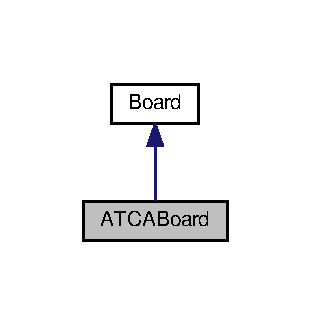
\includegraphics[width=149pt]{class_a_t_c_a_board__inherit__graph}
\end{center}
\end{figure}


Collaboration diagram for A\+T\+C\+A\+Board\+:\nopagebreak
\begin{figure}[H]
\begin{center}
\leavevmode
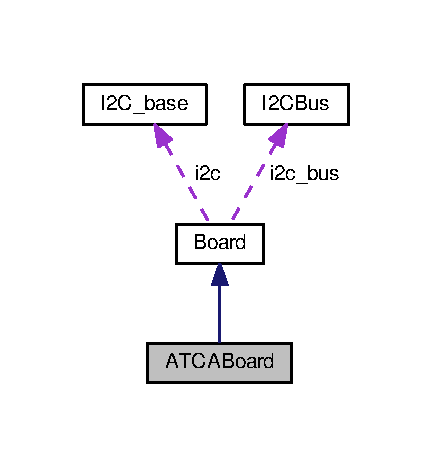
\includegraphics[width=208pt]{class_a_t_c_a_board__coll__graph}
\end{center}
\end{figure}
\subsection*{Public Member Functions}
\begin{DoxyCompactItemize}
\item 
\hyperlink{class_a_t_c_a_board_a4046dcaa2d61102e91005f2845e06201}{A\+T\+C\+A\+Board} (\hyperlink{class_i2_c__base}{I2\+C\+\_\+base} $\ast$i2c\+\_\+type)
\begin{DoxyCompactList}\small\item\em Class constructor. Full bus/device/register map is defined here. Also requests downstream bus from arbiter. \end{DoxyCompactList}\item 
\hyperlink{class_a_t_c_a_board_ac8d07dfe60a49f07a94a09868dc3637b}{A\+T\+C\+A\+Board} (std\+::string i2c\+\_\+string)
\begin{DoxyCompactList}\small\item\em Class constructor. Full bus/device/register map is defined here. Also requests downstream bus from arbiter. \end{DoxyCompactList}\item 
\hyperlink{class_a_t_c_a_board_a4f51f5462bd42562a1cdd20eb3a3bfeb}{$\sim$\+A\+T\+C\+A\+Board} (void)
\begin{DoxyCompactList}\small\item\em Class destructor. Gives up downstream bus to arbiter. \end{DoxyCompactList}\item 
std\+::unordered\+\_\+map$<$ std\+::string, \hyperlink{class_i2_c_bus}{I2\+C\+Bus} $\ast$ $>$ \hyperlink{class_a_t_c_a_board_a3926d4c4f9e4b98640b9b902b88ecb22}{get\+Map} (void)
\begin{DoxyCompactList}\small\item\em Get the map. \end{DoxyCompactList}\item 
void \hyperlink{class_a_t_c_a_board_a7aeb3e3e9488e3e016bc844b3eb0f36b}{set\+Bus} (std\+::string bus)
\begin{DoxyCompactList}\small\item\em Set bus to communicate over. \end{DoxyCompactList}\item 
void \hyperlink{class_a_t_c_a_board_ad0395aa7fe27ed6602ea55dfbe10b24d}{set\+Device} (std\+::string device)
\begin{DoxyCompactList}\small\item\em Set device to communicate to. \end{DoxyCompactList}\item 
void \hyperlink{class_a_t_c_a_board_ac7e7f32ba0c3583b67d8fa0c6a4703b7}{set\+Device} (std\+::string bus, std\+::string device)
\begin{DoxyCompactList}\small\item\em Set device to communicate to. \end{DoxyCompactList}\end{DoxyCompactItemize}
\subsection*{Additional Inherited Members}


\subsection{Detailed Description}


Definition at line 11 of file A\+T\+C\+A\+Board.\+hpp.



\subsection{Constructor \& Destructor Documentation}
\index{A\+T\+C\+A\+Board@{A\+T\+C\+A\+Board}!A\+T\+C\+A\+Board@{A\+T\+C\+A\+Board}}
\index{A\+T\+C\+A\+Board@{A\+T\+C\+A\+Board}!A\+T\+C\+A\+Board@{A\+T\+C\+A\+Board}}
\subsubsection[{\texorpdfstring{A\+T\+C\+A\+Board(\+I2\+C\+\_\+base $\ast$i2c\+\_\+type)}{ATCABoard(I2C_base *i2c_type)}}]{\setlength{\rightskip}{0pt plus 5cm}A\+T\+C\+A\+Board\+::\+A\+T\+C\+A\+Board (
\begin{DoxyParamCaption}
\item[{{\bf I2\+C\+\_\+base} $\ast$}]{i2c\+\_\+type}
\end{DoxyParamCaption}
)}\hypertarget{class_a_t_c_a_board_a4046dcaa2d61102e91005f2845e06201}{}\label{class_a_t_c_a_board_a4046dcaa2d61102e91005f2845e06201}


Class constructor. Full bus/device/register map is defined here. Also requests downstream bus from arbiter. 


\begin{DoxyParams}{Parameters}
{\em i2c\+\_\+type} & -\/ Pointer to \hyperlink{class_i2_c__base}{I2\+C\+\_\+base} transport object. \\
\hline
\end{DoxyParams}


Definition at line 15 of file A\+T\+C\+A\+Board.\+cpp.

\index{A\+T\+C\+A\+Board@{A\+T\+C\+A\+Board}!A\+T\+C\+A\+Board@{A\+T\+C\+A\+Board}}
\index{A\+T\+C\+A\+Board@{A\+T\+C\+A\+Board}!A\+T\+C\+A\+Board@{A\+T\+C\+A\+Board}}
\subsubsection[{\texorpdfstring{A\+T\+C\+A\+Board(std\+::string i2c\+\_\+string)}{ATCABoard(std::string i2c_string)}}]{\setlength{\rightskip}{0pt plus 5cm}A\+T\+C\+A\+Board\+::\+A\+T\+C\+A\+Board (
\begin{DoxyParamCaption}
\item[{std\+::string}]{i2c\+\_\+string}
\end{DoxyParamCaption}
)}\hypertarget{class_a_t_c_a_board_ac8d07dfe60a49f07a94a09868dc3637b}{}\label{class_a_t_c_a_board_ac8d07dfe60a49f07a94a09868dc3637b}


Class constructor. Full bus/device/register map is defined here. Also requests downstream bus from arbiter. 


\begin{DoxyParams}{Parameters}
{\em i2c\+\_\+type} & -\/ Pointer to \hyperlink{class_i2_c__base}{I2\+C\+\_\+base} transport object. \\
\hline
\end{DoxyParams}


Definition at line 48 of file A\+T\+C\+A\+Board.\+cpp.

\index{A\+T\+C\+A\+Board@{A\+T\+C\+A\+Board}!````~A\+T\+C\+A\+Board@{$\sim$\+A\+T\+C\+A\+Board}}
\index{````~A\+T\+C\+A\+Board@{$\sim$\+A\+T\+C\+A\+Board}!A\+T\+C\+A\+Board@{A\+T\+C\+A\+Board}}
\subsubsection[{\texorpdfstring{$\sim$\+A\+T\+C\+A\+Board(void)}{~ATCABoard(void)}}]{\setlength{\rightskip}{0pt plus 5cm}A\+T\+C\+A\+Board\+::$\sim$\+A\+T\+C\+A\+Board (
\begin{DoxyParamCaption}
\item[{void}]{}
\end{DoxyParamCaption}
)}\hypertarget{class_a_t_c_a_board_a4f51f5462bd42562a1cdd20eb3a3bfeb}{}\label{class_a_t_c_a_board_a4f51f5462bd42562a1cdd20eb3a3bfeb}


Class destructor. Gives up downstream bus to arbiter. 



Definition at line 91 of file A\+T\+C\+A\+Board.\+cpp.



\subsection{Member Function Documentation}
\index{A\+T\+C\+A\+Board@{A\+T\+C\+A\+Board}!get\+Map@{get\+Map}}
\index{get\+Map@{get\+Map}!A\+T\+C\+A\+Board@{A\+T\+C\+A\+Board}}
\subsubsection[{\texorpdfstring{get\+Map(void)}{getMap(void)}}]{\setlength{\rightskip}{0pt plus 5cm}std\+::unordered\+\_\+map$<$ std\+::string, {\bf I2\+C\+Bus} $\ast$ $>$ A\+T\+C\+A\+Board\+::get\+Map (
\begin{DoxyParamCaption}
\item[{void}]{}
\end{DoxyParamCaption}
)\hspace{0.3cm}{\ttfamily [virtual]}}\hypertarget{class_a_t_c_a_board_a3926d4c4f9e4b98640b9b902b88ecb22}{}\label{class_a_t_c_a_board_a3926d4c4f9e4b98640b9b902b88ecb22}


Get the map. 

\begin{DoxyReturn}{Returns}
Unordered map of string identifiers and \hyperlink{class_i2_c_bus}{I2\+C\+Bus} pointers. 
\end{DoxyReturn}


Implements \hyperlink{class_board_a7579517a69f81e2fcbe9e18857a11545}{Board}.



Definition at line 176 of file A\+T\+C\+A\+Board.\+cpp.

\index{A\+T\+C\+A\+Board@{A\+T\+C\+A\+Board}!set\+Bus@{set\+Bus}}
\index{set\+Bus@{set\+Bus}!A\+T\+C\+A\+Board@{A\+T\+C\+A\+Board}}
\subsubsection[{\texorpdfstring{set\+Bus(std\+::string bus)}{setBus(std::string bus)}}]{\setlength{\rightskip}{0pt plus 5cm}void A\+T\+C\+A\+Board\+::set\+Bus (
\begin{DoxyParamCaption}
\item[{std\+::string}]{bus}
\end{DoxyParamCaption}
)}\hypertarget{class_a_t_c_a_board_a7aeb3e3e9488e3e016bc844b3eb0f36b}{}\label{class_a_t_c_a_board_a7aeb3e3e9488e3e016bc844b3eb0f36b}


Set bus to communicate over. 


\begin{DoxyParams}{Parameters}
{\em bus} & -\/ String identifier for bus. \\
\hline
\end{DoxyParams}


Definition at line 142 of file A\+T\+C\+A\+Board.\+cpp.

\index{A\+T\+C\+A\+Board@{A\+T\+C\+A\+Board}!set\+Device@{set\+Device}}
\index{set\+Device@{set\+Device}!A\+T\+C\+A\+Board@{A\+T\+C\+A\+Board}}
\subsubsection[{\texorpdfstring{set\+Device(std\+::string device)}{setDevice(std::string device)}}]{\setlength{\rightskip}{0pt plus 5cm}void A\+T\+C\+A\+Board\+::set\+Device (
\begin{DoxyParamCaption}
\item[{std\+::string}]{device}
\end{DoxyParamCaption}
)}\hypertarget{class_a_t_c_a_board_ad0395aa7fe27ed6602ea55dfbe10b24d}{}\label{class_a_t_c_a_board_ad0395aa7fe27ed6602ea55dfbe10b24d}


Set device to communicate to. 


\begin{DoxyParams}{Parameters}
{\em device} & -\/ String identifier for device. \\
\hline
\end{DoxyParams}


Definition at line 152 of file A\+T\+C\+A\+Board.\+cpp.

\index{A\+T\+C\+A\+Board@{A\+T\+C\+A\+Board}!set\+Device@{set\+Device}}
\index{set\+Device@{set\+Device}!A\+T\+C\+A\+Board@{A\+T\+C\+A\+Board}}
\subsubsection[{\texorpdfstring{set\+Device(std\+::string bus, std\+::string device)}{setDevice(std::string bus, std::string device)}}]{\setlength{\rightskip}{0pt plus 5cm}void A\+T\+C\+A\+Board\+::set\+Device (
\begin{DoxyParamCaption}
\item[{std\+::string}]{bus, }
\item[{std\+::string}]{device}
\end{DoxyParamCaption}
)}\hypertarget{class_a_t_c_a_board_ac7e7f32ba0c3583b67d8fa0c6a4703b7}{}\label{class_a_t_c_a_board_ac7e7f32ba0c3583b67d8fa0c6a4703b7}


Set device to communicate to. 


\begin{DoxyParams}{Parameters}
{\em bus} & -\/ String identifier for bus. \\
\hline
{\em device} & -\/ String identifier for device. \\
\hline
\end{DoxyParams}


Definition at line 164 of file A\+T\+C\+A\+Board.\+cpp.



The documentation for this class was generated from the following files\+:\begin{DoxyCompactItemize}
\item 
include/\hyperlink{_a_t_c_a_board_8hpp}{A\+T\+C\+A\+Board.\+hpp}\item 
src/\hyperlink{_a_t_c_a_board_8cpp}{A\+T\+C\+A\+Board.\+cpp}\end{DoxyCompactItemize}

\hypertarget{classnlohmann_1_1basic__json}{}\section{nlohmann\+:\+:basic\+\_\+json$<$ Object\+Type, Array\+Type, String\+Type, Boolean\+Type, Number\+Integer\+Type, Number\+Unsigned\+Type, Number\+Float\+Type, Allocator\+Type, J\+S\+O\+N\+Serializer $>$ Class Template Reference}
\label{classnlohmann_1_1basic__json}\index{nlohmann\+::basic\+\_\+json$<$ Object\+Type, Array\+Type, String\+Type, Boolean\+Type, Number\+Integer\+Type, Number\+Unsigned\+Type, Number\+Float\+Type, Allocator\+Type, J\+S\+O\+N\+Serializer $>$@{nlohmann\+::basic\+\_\+json$<$ Object\+Type, Array\+Type, String\+Type, Boolean\+Type, Number\+Integer\+Type, Number\+Unsigned\+Type, Number\+Float\+Type, Allocator\+Type, J\+S\+O\+N\+Serializer $>$}}


a class to store J\+S\+ON values  




{\ttfamily \#include $<$json.\+hpp$>$}

\subsection*{Public Types}
\begin{DoxyCompactItemize}
\item 
using \hyperlink{classnlohmann_1_1basic__json_ae8cbef097f7da18a781fc86587de6b90}{value\+\_\+t} = \hyperlink{namespacenlohmann_1_1detail_a90aa5ef615aa8305e9ea20d8a947980f}{detail\+::value\+\_\+t}
\item 
using \hyperlink{classnlohmann_1_1basic__json_a32d3ee58bf01b28d11366f307518bf34}{json\+\_\+pointer} = \+::\hyperlink{classnlohmann_1_1json__pointer}{nlohmann\+::json\+\_\+pointer}
\item 
{\footnotesize template$<$typename T , typename S\+F\+I\+N\+AE $>$ }\\using \hyperlink{classnlohmann_1_1basic__json_a7768841baaaa7a21098a401c932efaff}{json\+\_\+serializer} = J\+S\+O\+N\+Serializer$<$ T, S\+F\+I\+N\+AE $>$
\item 
using \hyperlink{classnlohmann_1_1basic__json_a670f6a0eb3d1e0ffd00c27d35472ccc9}{initializer\+\_\+list\+\_\+t} = std\+::initializer\+\_\+list$<$ \hyperlink{classnlohmann_1_1detail_1_1json__ref}{detail\+::json\+\_\+ref}$<$ \hyperlink{classnlohmann_1_1basic__json}{basic\+\_\+json} $>$$>$
\item 
using \hyperlink{classnlohmann_1_1basic__json_aaceba2e4cf75fc983bb75c78c8742e65}{parse\+\_\+event\+\_\+t} = typename \hyperlink{classnlohmann_1_1detail_1_1parser_a37ac88c864dda495f72cb62776b0bebe}{parser\+::parse\+\_\+event\+\_\+t}
\item 
using \hyperlink{classnlohmann_1_1basic__json_ab4f78c5f9fd25172eeec84482e03f5b7}{parser\+\_\+callback\+\_\+t} = typename \hyperlink{classnlohmann_1_1detail_1_1parser_ad250ad4f2b4af4a497e727c963162ff1}{parser\+::parser\+\_\+callback\+\_\+t}
\begin{DoxyCompactList}\small\item\em per-\/element parser callback type \end{DoxyCompactList}\end{DoxyCompactItemize}
\subsection*{Public Member Functions}
\begin{DoxyCompactItemize}
\item 
const char $\ast$ \hyperlink{classnlohmann_1_1basic__json_ac1d94c098e7edae0fc36185a84196a6a}{type\+\_\+name} () const 
\begin{DoxyCompactList}\small\item\em return the type as string \end{DoxyCompactList}\end{DoxyCompactItemize}
\subsection*{Static Public Member Functions}
\begin{DoxyCompactItemize}
\item 
static \hyperlink{classnlohmann_1_1basic__json_a86ce930490cf7773b26f5ef49c04a350}{allocator\+\_\+type} \hyperlink{classnlohmann_1_1basic__json_af4ac14224fbdd29d3547fcb11bb55c8f}{get\+\_\+allocator} ()
\begin{DoxyCompactList}\small\item\em returns the allocator associated with the container \end{DoxyCompactList}\item 
static \hyperlink{classnlohmann_1_1basic__json}{basic\+\_\+json} \hyperlink{classnlohmann_1_1basic__json_aef6d0eeccee7c5c7e1317c2ea1607fab}{meta} ()
\begin{DoxyCompactList}\small\item\em returns version information on the library \end{DoxyCompactList}\end{DoxyCompactItemize}
\subsection*{Friends}
\begin{DoxyCompactItemize}
\item 
{\footnotesize template$<$detail\+::value\+\_\+t $>$ }\\struct \hyperlink{classnlohmann_1_1basic__json_a6275ed57bae6866cdf5db5370a7ad47c}{detail\+::external\+\_\+constructor}
\item 
{\footnotesize template$<$typename Basic\+Json\+Type $>$ }\\class \hyperlink{classnlohmann_1_1basic__json_a842e5c7ca096025c18b11e715d3401f4}{\+::nlohmann\+::detail\+::iter\+\_\+impl}
\item 
{\footnotesize template$<$typename Basic\+Json\+Type , typename Char\+Type $>$ }\\class \hyperlink{classnlohmann_1_1basic__json_a69d491bbda88ade6d3c7a2b11309e8bf}{\+::nlohmann\+::detail\+::binary\+\_\+writer}
\end{DoxyCompactItemize}
\subsection*{exceptions}
\label{_amgrp19ad27801b95bd1f2c6c2bf83dbb7515}%
Classes to implement user-\/defined exceptions. \begin{DoxyCompactItemize}
\item 
using \hyperlink{classnlohmann_1_1basic__json_a9a0aced019cb1d65bb49703406c84970}{exception} = \hyperlink{classnlohmann_1_1detail_1_1exception}{detail\+::exception}
\begin{DoxyCompactList}\small\item\em general exception of the \hyperlink{classnlohmann_1_1basic__json}{basic\+\_\+json} class \end{DoxyCompactList}\item 
using \hyperlink{classnlohmann_1_1basic__json_af1efc2468e6022be6e35fc2944cabe4d}{parse\+\_\+error} = \hyperlink{classnlohmann_1_1detail_1_1parse__error}{detail\+::parse\+\_\+error}
\begin{DoxyCompactList}\small\item\em exception indicating a parse error \end{DoxyCompactList}\item 
using \hyperlink{classnlohmann_1_1basic__json_ac13d32f7cbd02d616e71d8dc30dadcbf}{invalid\+\_\+iterator} = \hyperlink{classnlohmann_1_1detail_1_1invalid__iterator}{detail\+::invalid\+\_\+iterator}
\begin{DoxyCompactList}\small\item\em exception indicating errors with iterators \end{DoxyCompactList}\item 
using \hyperlink{classnlohmann_1_1basic__json_a4010e8e268fefd86da773c10318f2902}{type\+\_\+error} = \hyperlink{classnlohmann_1_1detail_1_1type__error}{detail\+::type\+\_\+error}
\begin{DoxyCompactList}\small\item\em exception indicating executing a member function with a wrong type \end{DoxyCompactList}\item 
using \hyperlink{classnlohmann_1_1basic__json_a28f7c2f087274a0012eb7a2333ee1580}{out\+\_\+of\+\_\+range} = \hyperlink{classnlohmann_1_1detail_1_1out__of__range}{detail\+::out\+\_\+of\+\_\+range}
\begin{DoxyCompactList}\small\item\em exception indicating access out of the defined range \end{DoxyCompactList}\item 
using \hyperlink{classnlohmann_1_1basic__json_a3333a5a8714912adda33a35b369f7b3d}{other\+\_\+error} = \hyperlink{classnlohmann_1_1detail_1_1other__error}{detail\+::other\+\_\+error}
\begin{DoxyCompactList}\small\item\em exception indicating other errors \end{DoxyCompactList}\end{DoxyCompactItemize}
\subsection*{container types}
\label{_amgrp6618fa684bc6d5a05e2c88bfff1c0d66}%
The canonic container types to use \hyperlink{classnlohmann_1_1basic__json}{basic\+\_\+json} like any other S\+TL container. \begin{DoxyCompactItemize}
\item 
using \hyperlink{classnlohmann_1_1basic__json_a2b3297873b70c080837e8eedc4fec32f}{value\+\_\+type} = \hyperlink{classnlohmann_1_1basic__json}{basic\+\_\+json}
\begin{DoxyCompactList}\small\item\em the type of elements in a \hyperlink{classnlohmann_1_1basic__json}{basic\+\_\+json} container \end{DoxyCompactList}\item 
using \hyperlink{classnlohmann_1_1basic__json_ac6a5eddd156c776ac75ff54cfe54a5bc}{reference} = \hyperlink{classnlohmann_1_1basic__json_a2b3297873b70c080837e8eedc4fec32f}{value\+\_\+type} \&
\begin{DoxyCompactList}\small\item\em the type of an element reference \end{DoxyCompactList}\item 
using \hyperlink{classnlohmann_1_1basic__json_a4057c5425f4faacfe39a8046871786ca}{const\+\_\+reference} = const \hyperlink{classnlohmann_1_1basic__json_a2b3297873b70c080837e8eedc4fec32f}{value\+\_\+type} \&
\begin{DoxyCompactList}\small\item\em the type of an element const reference \end{DoxyCompactList}\item 
using \hyperlink{classnlohmann_1_1basic__json_afe7c1303357e19cea9527af4e9a31d8f}{difference\+\_\+type} = std\+::ptrdiff\+\_\+t
\begin{DoxyCompactList}\small\item\em a type to represent differences between iterators \end{DoxyCompactList}\item 
using \hyperlink{classnlohmann_1_1basic__json_a39f2cd0b58106097e0e67bf185cc519b}{size\+\_\+type} = std\+::size\+\_\+t
\begin{DoxyCompactList}\small\item\em a type to represent container sizes \end{DoxyCompactList}\item 
using \hyperlink{classnlohmann_1_1basic__json_a86ce930490cf7773b26f5ef49c04a350}{allocator\+\_\+type} = Allocator\+Type$<$ \hyperlink{classnlohmann_1_1basic__json}{basic\+\_\+json} $>$
\begin{DoxyCompactList}\small\item\em the allocator type \end{DoxyCompactList}\item 
using \hyperlink{classnlohmann_1_1basic__json_aefee1f777198c68724bd127e0c8abbe4}{pointer} = typename std\+::allocator\+\_\+traits$<$ \hyperlink{classnlohmann_1_1basic__json_a86ce930490cf7773b26f5ef49c04a350}{allocator\+\_\+type} $>$\+::\hyperlink{classnlohmann_1_1basic__json_aefee1f777198c68724bd127e0c8abbe4}{pointer}
\begin{DoxyCompactList}\small\item\em the type of an element pointer \end{DoxyCompactList}\item 
using \hyperlink{classnlohmann_1_1basic__json_aff3d5cd2a75612364b888d8693231b58}{const\+\_\+pointer} = typename std\+::allocator\+\_\+traits$<$ \hyperlink{classnlohmann_1_1basic__json_a86ce930490cf7773b26f5ef49c04a350}{allocator\+\_\+type} $>$\+::\hyperlink{classnlohmann_1_1basic__json_aff3d5cd2a75612364b888d8693231b58}{const\+\_\+pointer}
\begin{DoxyCompactList}\small\item\em the type of an element const pointer \end{DoxyCompactList}\item 
using \hyperlink{classnlohmann_1_1basic__json_a099316232c76c034030a38faa6e34dca}{iterator} = \hyperlink{classnlohmann_1_1detail_1_1iter__impl}{iter\+\_\+impl}$<$ \hyperlink{classnlohmann_1_1basic__json}{basic\+\_\+json} $>$
\begin{DoxyCompactList}\small\item\em an iterator for a \hyperlink{classnlohmann_1_1basic__json}{basic\+\_\+json} container \end{DoxyCompactList}\item 
using \hyperlink{classnlohmann_1_1basic__json_a41a70cf9993951836d129bb1c2b3126a}{const\+\_\+iterator} = \hyperlink{classnlohmann_1_1detail_1_1iter__impl}{iter\+\_\+impl}$<$ const \hyperlink{classnlohmann_1_1basic__json}{basic\+\_\+json} $>$
\begin{DoxyCompactList}\small\item\em a const iterator for a \hyperlink{classnlohmann_1_1basic__json}{basic\+\_\+json} container \end{DoxyCompactList}\item 
using \hyperlink{classnlohmann_1_1basic__json_ac223d5560c2b05a208c88de67376c5f2}{reverse\+\_\+iterator} = \hyperlink{classnlohmann_1_1detail_1_1json__reverse__iterator}{json\+\_\+reverse\+\_\+iterator}$<$ typename \hyperlink{classnlohmann_1_1basic__json_a099316232c76c034030a38faa6e34dca}{basic\+\_\+json\+::iterator} $>$
\begin{DoxyCompactList}\small\item\em a reverse iterator for a \hyperlink{classnlohmann_1_1basic__json}{basic\+\_\+json} container \end{DoxyCompactList}\item 
using \hyperlink{classnlohmann_1_1basic__json_a72be3c24bfa24f0993d6c11af03e7404}{const\+\_\+reverse\+\_\+iterator} = \hyperlink{classnlohmann_1_1detail_1_1json__reverse__iterator}{json\+\_\+reverse\+\_\+iterator}$<$ typename \hyperlink{classnlohmann_1_1basic__json_a41a70cf9993951836d129bb1c2b3126a}{basic\+\_\+json\+::const\+\_\+iterator} $>$
\begin{DoxyCompactList}\small\item\em a const reverse iterator for a \hyperlink{classnlohmann_1_1basic__json}{basic\+\_\+json} container \end{DoxyCompactList}\end{DoxyCompactItemize}
\subsection*{J\+S\+ON value data types}
\label{_amgrpbddfba6d49869d59bfd397e65b8cba87}%
The data types to store a J\+S\+ON value. These types are derived from the template arguments passed to class \hyperlink{classnlohmann_1_1basic__json}{basic\+\_\+json}. \begin{DoxyCompactItemize}
\item 
using \hyperlink{classnlohmann_1_1basic__json_a3cdea044cc3ecba1c4f9874a89daf6e4}{object\+\_\+t} = Object\+Type$<$ String\+Type, \hyperlink{classnlohmann_1_1basic__json}{basic\+\_\+json}, std\+::less$<$ String\+Type $>$, Allocator\+Type$<$ std\+::pair$<$ const String\+Type, \hyperlink{classnlohmann_1_1basic__json}{basic\+\_\+json} $>$$>$$>$
\begin{DoxyCompactList}\small\item\em a type for an object \end{DoxyCompactList}\item 
using \hyperlink{classnlohmann_1_1basic__json_a4c409f1b6d9caf3412c78af9a5883fed}{array\+\_\+t} = Array\+Type$<$ \hyperlink{classnlohmann_1_1basic__json}{basic\+\_\+json}, Allocator\+Type$<$ \hyperlink{classnlohmann_1_1basic__json}{basic\+\_\+json} $>$$>$
\begin{DoxyCompactList}\small\item\em a type for an array \end{DoxyCompactList}\item 
using \hyperlink{classnlohmann_1_1basic__json_a61f8566a1a85a424c7266fb531dca005}{string\+\_\+t} = String\+Type
\begin{DoxyCompactList}\small\item\em a type for a string \end{DoxyCompactList}\item 
using \hyperlink{classnlohmann_1_1basic__json_a4c919102a9b4fe0d588af64801436082}{boolean\+\_\+t} = Boolean\+Type
\begin{DoxyCompactList}\small\item\em a type for a boolean \end{DoxyCompactList}\item 
using \hyperlink{classnlohmann_1_1basic__json_a98e611d67b7bd75307de99c9358ab2dc}{number\+\_\+integer\+\_\+t} = Number\+Integer\+Type
\begin{DoxyCompactList}\small\item\em a type for a number (integer) \end{DoxyCompactList}\item 
using \hyperlink{classnlohmann_1_1basic__json_ab906e29b5d83ac162e823ada2156b989}{number\+\_\+unsigned\+\_\+t} = Number\+Unsigned\+Type
\begin{DoxyCompactList}\small\item\em a type for a number (unsigned) \end{DoxyCompactList}\item 
using \hyperlink{classnlohmann_1_1basic__json_a88d6103cb3620410b35200ee8e313d97}{number\+\_\+float\+\_\+t} = Number\+Float\+Type
\begin{DoxyCompactList}\small\item\em a type for a number (floating-\/point) \end{DoxyCompactList}\end{DoxyCompactItemize}
\subsection*{constructors and destructors}
\label{_amgrpd94b4d3d0135946bb7bdf25e48755337}%
Constructors of class \hyperlink{classnlohmann_1_1basic__json}{basic\+\_\+json}, copy/move constructor, copy assignment, static functions creating objects, and the destructor. \begin{DoxyCompactItemize}
\item 
static \hyperlink{classnlohmann_1_1basic__json}{basic\+\_\+json} \hyperlink{classnlohmann_1_1basic__json_aa80485befaffcadaa39965494e0b4d2e}{array} (\hyperlink{classnlohmann_1_1basic__json_a670f6a0eb3d1e0ffd00c27d35472ccc9}{initializer\+\_\+list\+\_\+t} init=\{\})
\begin{DoxyCompactList}\small\item\em explicitly create an array from an initializer list \end{DoxyCompactList}\item 
static \hyperlink{classnlohmann_1_1basic__json}{basic\+\_\+json} \hyperlink{classnlohmann_1_1basic__json_aa13f7c0615867542ce80337cbcf13ada}{object} (\hyperlink{classnlohmann_1_1basic__json_a670f6a0eb3d1e0ffd00c27d35472ccc9}{initializer\+\_\+list\+\_\+t} init=\{\})
\begin{DoxyCompactList}\small\item\em explicitly create an object from an initializer list \end{DoxyCompactList}\item 
\hyperlink{classnlohmann_1_1basic__json_aed115142bd0c6c66c864700e0467df55}{basic\+\_\+json} (const \hyperlink{namespacenlohmann_1_1detail_a90aa5ef615aa8305e9ea20d8a947980f}{value\+\_\+t} v)
\begin{DoxyCompactList}\small\item\em create an empty value with a given type \end{DoxyCompactList}\item 
\hyperlink{classnlohmann_1_1basic__json_ae9be9e956bfc4658f35d17c6aa72b063}{basic\+\_\+json} (std\+::nullptr\+\_\+t=nullptr) noexcept
\begin{DoxyCompactList}\small\item\em create a null object \end{DoxyCompactList}\item 
{\footnotesize template$<$typename Compatible\+Type , typename U  = detail\+::uncvref\+\_\+t$<$\+Compatible\+Type$>$, detail\+::enable\+\_\+if\+\_\+t$<$ not std\+::is\+\_\+base\+\_\+of$<$ std\+::istream, U $>$\+::value andnot std\+::is\+\_\+same$<$ U, basic\+\_\+json\+\_\+t $>$\+::value andnot detail\+::is\+\_\+basic\+\_\+json\+\_\+nested\+\_\+type$<$ basic\+\_\+json\+\_\+t, U $>$\+::value anddetail\+::has\+\_\+to\+\_\+json$<$ basic\+\_\+json, U $>$\+::value, int $>$  = 0$>$ }\\\hyperlink{classnlohmann_1_1basic__json_a7639e0834df2bc719a04ffea89b31abc}{basic\+\_\+json} (Compatible\+Type \&\&val) noexcept(noexcept(J\+S\+O\+N\+Serializer$<$ U $>$\+::to\+\_\+json(std\+::declval$<$ basic\+\_\+json\+\_\+t \& $>$(), std\+::forward$<$ Compatible\+Type $>$(val))))
\begin{DoxyCompactList}\small\item\em create a J\+S\+ON value \end{DoxyCompactList}\item 
\hyperlink{classnlohmann_1_1basic__json_ab5dfd9a2b2663b219641cb7fe59b6da2}{basic\+\_\+json} (\hyperlink{classnlohmann_1_1basic__json_a670f6a0eb3d1e0ffd00c27d35472ccc9}{initializer\+\_\+list\+\_\+t} init, bool type\+\_\+deduction=true, \hyperlink{namespacenlohmann_1_1detail_a90aa5ef615aa8305e9ea20d8a947980f}{value\+\_\+t} manual\+\_\+type=\hyperlink{namespacenlohmann_1_1detail_a90aa5ef615aa8305e9ea20d8a947980faf1f713c9e000f5d3f280adbd124df4f5}{value\+\_\+t\+::array})
\begin{DoxyCompactList}\small\item\em create a container (array or object) from an initializer list \end{DoxyCompactList}\item 
\hyperlink{classnlohmann_1_1basic__json_ab6816ae5100409254ed0a8bc21c387bb}{basic\+\_\+json} (\hyperlink{classnlohmann_1_1basic__json_a39f2cd0b58106097e0e67bf185cc519b}{size\+\_\+type} cnt, const \hyperlink{classnlohmann_1_1basic__json}{basic\+\_\+json} \&val)
\begin{DoxyCompactList}\small\item\em construct an array with count copies of given value \end{DoxyCompactList}\item 
{\footnotesize template$<$class Input\+IT , typename std\+::enable\+\_\+if$<$ std\+::is\+\_\+same$<$ Input\+I\+T, typename basic\+\_\+json\+\_\+t\+::iterator $>$\+::value orstd\+::is\+\_\+same$<$ Input\+I\+T, typename basic\+\_\+json\+\_\+t\+::const\+\_\+iterator $>$\+::value, int $>$\+::type  = 0$>$ }\\\hyperlink{classnlohmann_1_1basic__json_abe197e9f3184487805cfb5bba6fd5938}{basic\+\_\+json} (Input\+IT first, Input\+IT last)
\begin{DoxyCompactList}\small\item\em construct a J\+S\+ON container given an iterator range \end{DoxyCompactList}\item 
\hyperlink{classnlohmann_1_1basic__json_a2be0a411fe0e3418abc4c58889be4943}{basic\+\_\+json} (const \hyperlink{classnlohmann_1_1detail_1_1json__ref}{detail\+::json\+\_\+ref}$<$ \hyperlink{classnlohmann_1_1basic__json}{basic\+\_\+json} $>$ \&ref)
\item 
\hyperlink{classnlohmann_1_1basic__json_af5de621bcf646c332343f9c1e011126c}{basic\+\_\+json} (const \hyperlink{classnlohmann_1_1basic__json}{basic\+\_\+json} \&other)
\begin{DoxyCompactList}\small\item\em copy constructor \end{DoxyCompactList}\item 
\hyperlink{classnlohmann_1_1basic__json_a9a06d1efd50a00f4889f831f851ce124}{basic\+\_\+json} (\hyperlink{classnlohmann_1_1basic__json}{basic\+\_\+json} \&\&other) noexcept
\begin{DoxyCompactList}\small\item\em move constructor \end{DoxyCompactList}\item 
\hyperlink{classnlohmann_1_1basic__json_ac6a5eddd156c776ac75ff54cfe54a5bc}{reference} \& \hyperlink{classnlohmann_1_1basic__json_a175607715d6c65e8901038ebb629a5b9}{operator=} (\hyperlink{classnlohmann_1_1basic__json}{basic\+\_\+json} other) noexcept(std\+::is\+\_\+nothrow\+\_\+move\+\_\+constructible$<$ \hyperlink{namespacenlohmann_1_1detail_a90aa5ef615aa8305e9ea20d8a947980f}{value\+\_\+t} $>$\+::\hyperlink{classnlohmann_1_1basic__json_a9fa223b26419f018f9b18cc516e3a8e5}{value} andstd\+::is\+\_\+nothrow\+\_\+move\+\_\+assignable$<$ \hyperlink{namespacenlohmann_1_1detail_a90aa5ef615aa8305e9ea20d8a947980f}{value\+\_\+t} $>$\+::\hyperlink{classnlohmann_1_1basic__json_a9fa223b26419f018f9b18cc516e3a8e5}{value} andstd\+::is\+\_\+nothrow\+\_\+move\+\_\+constructible$<$ json\+\_\+value $>$\+::\hyperlink{classnlohmann_1_1basic__json_a9fa223b26419f018f9b18cc516e3a8e5}{value} andstd\+::is\+\_\+nothrow\+\_\+move\+\_\+assignable$<$ json\+\_\+value $>$\+::\hyperlink{classnlohmann_1_1basic__json_a9fa223b26419f018f9b18cc516e3a8e5}{value})
\begin{DoxyCompactList}\small\item\em copy assignment \end{DoxyCompactList}\item 
\hyperlink{classnlohmann_1_1basic__json_a42347bbce75ba5571e292a3540af30e0}{$\sim$basic\+\_\+json} ()
\begin{DoxyCompactList}\small\item\em destructor \end{DoxyCompactList}\end{DoxyCompactItemize}
\subsection*{object inspection}
\label{_amgrpbbb01a37b8f261ae5b5799058dcac1a0}%
Functions to inspect the type of a J\+S\+ON value. \begin{DoxyCompactItemize}
\item 
\hyperlink{classnlohmann_1_1basic__json_a61f8566a1a85a424c7266fb531dca005}{string\+\_\+t} \hyperlink{classnlohmann_1_1basic__json_ae5bfe31e51a06f32c273a3e79a4ea872}{dump} (const int indent=-\/1, const char indent\+\_\+char= \textquotesingle{} \textquotesingle{}, const bool ensure\+\_\+ascii=false) const 
\begin{DoxyCompactList}\small\item\em serialization \end{DoxyCompactList}\item 
constexpr \hyperlink{namespacenlohmann_1_1detail_a90aa5ef615aa8305e9ea20d8a947980f}{value\+\_\+t} \hyperlink{classnlohmann_1_1basic__json_a2b2d781d7f2a4ee41bc0016e931cadf7}{type} () const noexcept
\begin{DoxyCompactList}\small\item\em return the type of the J\+S\+ON value (explicit) \end{DoxyCompactList}\item 
constexpr bool \hyperlink{classnlohmann_1_1basic__json_a6362b88718eb5c6d4fed6a61eed44b95}{is\+\_\+primitive} () const noexcept
\begin{DoxyCompactList}\small\item\em return whether type is primitive \end{DoxyCompactList}\item 
constexpr bool \hyperlink{classnlohmann_1_1basic__json_a9f68a0af820c3ced7f9d17851ce4c22d}{is\+\_\+structured} () const noexcept
\begin{DoxyCompactList}\small\item\em return whether type is structured \end{DoxyCompactList}\item 
constexpr bool \hyperlink{classnlohmann_1_1basic__json_a8faa039ca82427ed29c486ffd00600c3}{is\+\_\+null} () const noexcept
\begin{DoxyCompactList}\small\item\em return whether value is null \end{DoxyCompactList}\item 
constexpr bool \hyperlink{classnlohmann_1_1basic__json_a943e8cb182d0f2365c76d64b42eaa6fd}{is\+\_\+boolean} () const noexcept
\begin{DoxyCompactList}\small\item\em return whether value is a boolean \end{DoxyCompactList}\item 
constexpr bool \hyperlink{classnlohmann_1_1basic__json_a2b9852390abb4b1ef5fac6984e2fc0f3}{is\+\_\+number} () const noexcept
\begin{DoxyCompactList}\small\item\em return whether value is a number \end{DoxyCompactList}\item 
constexpr bool \hyperlink{classnlohmann_1_1basic__json_abac8af76067f1e8fdca9052882c74428}{is\+\_\+number\+\_\+integer} () const noexcept
\begin{DoxyCompactList}\small\item\em return whether value is an integer number \end{DoxyCompactList}\item 
constexpr bool \hyperlink{classnlohmann_1_1basic__json_abc7378cba0613a78b9aad1c8e7044bb0}{is\+\_\+number\+\_\+unsigned} () const noexcept
\begin{DoxyCompactList}\small\item\em return whether value is an unsigned integer number \end{DoxyCompactList}\item 
constexpr bool \hyperlink{classnlohmann_1_1basic__json_a33b4bf898b857c962e798fc7f6e86e70}{is\+\_\+number\+\_\+float} () const noexcept
\begin{DoxyCompactList}\small\item\em return whether value is a floating-\/point number \end{DoxyCompactList}\item 
constexpr bool \hyperlink{classnlohmann_1_1basic__json_af8f511af124e82e4579f444b4175787c}{is\+\_\+object} () const noexcept
\begin{DoxyCompactList}\small\item\em return whether value is an object \end{DoxyCompactList}\item 
constexpr bool \hyperlink{classnlohmann_1_1basic__json_aef9ce5dd2381caee1f8ddcdb5bdd9c65}{is\+\_\+array} () const noexcept
\begin{DoxyCompactList}\small\item\em return whether value is an array \end{DoxyCompactList}\item 
constexpr bool \hyperlink{classnlohmann_1_1basic__json_a69b596a4a6683b362095c9a139637396}{is\+\_\+string} () const noexcept
\begin{DoxyCompactList}\small\item\em return whether value is a string \end{DoxyCompactList}\item 
constexpr bool \hyperlink{classnlohmann_1_1basic__json_aabe623bc8304c2ba92d96d91f390fab4}{is\+\_\+discarded} () const noexcept
\begin{DoxyCompactList}\small\item\em return whether value is discarded \end{DoxyCompactList}\item 
constexpr \hyperlink{classnlohmann_1_1basic__json_a26ef3058e249f82a04f8ec18f7419027}{operator value\+\_\+t} () const noexcept
\begin{DoxyCompactList}\small\item\em return the type of the J\+S\+ON value (implicit) \end{DoxyCompactList}\end{DoxyCompactItemize}
\subsection*{value access}
\label{_amgrpd8f53c9caf18314e5b3f758245606995}%
Direct access to the stored value of a J\+S\+ON value. \begin{DoxyCompactItemize}
\item 
{\footnotesize template$<$typename Basic\+Json\+Type , detail\+::enable\+\_\+if\+\_\+t$<$ std\+::is\+\_\+same$<$ typename std\+::remove\+\_\+const$<$ Basic\+Json\+Type $>$\+::type, basic\+\_\+json\+\_\+t $>$\+::value, int $>$  = 0$>$ }\\\hyperlink{classnlohmann_1_1basic__json}{basic\+\_\+json} \hyperlink{classnlohmann_1_1basic__json_ac41d1fda870c3f3c4ead932c2e3ab61f}{get} () const 
\begin{DoxyCompactList}\small\item\em get special-\/case overload \end{DoxyCompactList}\item 
{\footnotesize template$<$typename Value\+Type\+CV , typename Value\+Type  = detail\+::uncvref\+\_\+t$<$\+Value\+Type\+C\+V$>$, detail\+::enable\+\_\+if\+\_\+t$<$ not std\+::is\+\_\+same$<$ basic\+\_\+json\+\_\+t, Value\+Type $>$\+::value anddetail\+::has\+\_\+from\+\_\+json$<$ basic\+\_\+json\+\_\+t, Value\+Type $>$\+::value andnot detail\+::has\+\_\+non\+\_\+default\+\_\+from\+\_\+json$<$ basic\+\_\+json\+\_\+t, Value\+Type $>$\+::value, int $>$  = 0$>$ }\\Value\+Type \hyperlink{classnlohmann_1_1basic__json_aa6602bb24022183ab989439e19345d08}{get} () const noexcept(noexcept(J\+S\+O\+N\+Serializer$<$ Value\+Type $>$\+::from\+\_\+json(std\+::declval$<$ const basic\+\_\+json\+\_\+t \& $>$(), std\+::declval$<$ Value\+Type \& $>$())))
\begin{DoxyCompactList}\small\item\em get a value (explicit) \end{DoxyCompactList}\item 
{\footnotesize template$<$typename Value\+Type\+CV , typename Value\+Type  = detail\+::uncvref\+\_\+t$<$\+Value\+Type\+C\+V$>$, detail\+::enable\+\_\+if\+\_\+t$<$ not std\+::is\+\_\+same$<$ basic\+\_\+json\+\_\+t, Value\+Type $>$\+::value anddetail\+::has\+\_\+non\+\_\+default\+\_\+from\+\_\+json$<$ basic\+\_\+json\+\_\+t, Value\+Type $>$\+::value, int $>$  = 0$>$ }\\Value\+Type \hyperlink{classnlohmann_1_1basic__json_a5afa21d477e13fa7a3dcd7ea66c48b52}{get} () const noexcept(noexcept(J\+S\+O\+N\+Serializer$<$ Value\+Type\+CV $>$\+::from\+\_\+json(std\+::declval$<$ const basic\+\_\+json\+\_\+t \& $>$())))
\begin{DoxyCompactList}\small\item\em get a value (explicit); special case \end{DoxyCompactList}\item 
{\footnotesize template$<$typename Pointer\+Type , typename std\+::enable\+\_\+if$<$ std\+::is\+\_\+pointer$<$ Pointer\+Type $>$\+::value, int $>$\+::type  = 0$>$ }\\Pointer\+Type \hyperlink{classnlohmann_1_1basic__json_a64135c19425f00b346d8ed63a23db334}{get} () noexcept
\begin{DoxyCompactList}\small\item\em get a pointer value (explicit) \end{DoxyCompactList}\item 
{\footnotesize template$<$typename Pointer\+Type , typename std\+::enable\+\_\+if$<$ std\+::is\+\_\+pointer$<$ Pointer\+Type $>$\+::value, int $>$\+::type  = 0$>$ }\\constexpr const Pointer\+Type \hyperlink{classnlohmann_1_1basic__json_a44a090c15a67b9f02e579b6e17ef0e1b}{get} () const noexcept
\begin{DoxyCompactList}\small\item\em get a pointer value (explicit) \end{DoxyCompactList}\item 
{\footnotesize template$<$typename Pointer\+Type , typename std\+::enable\+\_\+if$<$ std\+::is\+\_\+pointer$<$ Pointer\+Type $>$\+::value, int $>$\+::type  = 0$>$ }\\Pointer\+Type \hyperlink{classnlohmann_1_1basic__json_aefa46bd2d96bb77a38d1c8b431eab44f}{get\+\_\+ptr} () noexcept
\begin{DoxyCompactList}\small\item\em get a pointer value (implicit) \end{DoxyCompactList}\item 
{\footnotesize template$<$typename Pointer\+Type , typename std\+::enable\+\_\+if$<$ std\+::is\+\_\+pointer$<$ Pointer\+Type $>$\+::value andstd\+::is\+\_\+const$<$ typename std\+::remove\+\_\+pointer$<$ Pointer\+Type $>$\+::type $>$\+::value, int $>$\+::type  = 0$>$ }\\constexpr const Pointer\+Type \hyperlink{classnlohmann_1_1basic__json_a14abd48803a8d5447faf5f583fa8e2a1}{get\+\_\+ptr} () const noexcept
\begin{DoxyCompactList}\small\item\em get a pointer value (implicit) \end{DoxyCompactList}\item 
{\footnotesize template$<$typename Reference\+Type , typename std\+::enable\+\_\+if$<$ std\+::is\+\_\+reference$<$ Reference\+Type $>$\+::value, int $>$\+::type  = 0$>$ }\\Reference\+Type \hyperlink{classnlohmann_1_1basic__json_afbd800010b67619463c0fce6e74f7878}{get\+\_\+ref} ()
\begin{DoxyCompactList}\small\item\em get a reference value (implicit) \end{DoxyCompactList}\item 
{\footnotesize template$<$typename Reference\+Type , typename std\+::enable\+\_\+if$<$ std\+::is\+\_\+reference$<$ Reference\+Type $>$\+::value andstd\+::is\+\_\+const$<$ typename std\+::remove\+\_\+reference$<$ Reference\+Type $>$\+::type $>$\+::value, int $>$\+::type  = 0$>$ }\\Reference\+Type \hyperlink{classnlohmann_1_1basic__json_a87e9e9cb2556fabfe042a4fabfc2c952}{get\+\_\+ref} () const 
\begin{DoxyCompactList}\small\item\em get a reference value (implicit) \end{DoxyCompactList}\item 
{\footnotesize template$<$typename Value\+Type , typename std\+::enable\+\_\+if$<$ not std\+::is\+\_\+pointer$<$ Value\+Type $>$\+::value andnot std\+::is\+\_\+same$<$ Value\+Type, detail\+::json\+\_\+ref$<$ basic\+\_\+json $>$$>$\+::value andnot std\+::is\+\_\+same$<$ Value\+Type, typename string\+\_\+t\+::value\+\_\+type $>$\+::valueand not std\+::is\+\_\+same$<$ Value\+Type, std\+::initializer\+\_\+list$<$ typename string\+\_\+t\+::value\+\_\+type $>$$>$\+::value, int $>$\+::type  = 0$>$ }\\\hyperlink{classnlohmann_1_1basic__json_a9cbcce20b78708de25c7ccb60c4ca7c5}{operator Value\+Type} () const 
\begin{DoxyCompactList}\small\item\em get a value (implicit) \end{DoxyCompactList}\end{DoxyCompactItemize}
\subsection*{element access}
\label{_amgrpf68418821a90b03a001117a613b131dd}%
Access to the J\+S\+ON value. \begin{DoxyCompactItemize}
\item 
\hyperlink{classnlohmann_1_1basic__json_ac6a5eddd156c776ac75ff54cfe54a5bc}{reference} \hyperlink{classnlohmann_1_1basic__json_a73ae333487310e3302135189ce8ff5d8}{at} (\hyperlink{classnlohmann_1_1basic__json_a39f2cd0b58106097e0e67bf185cc519b}{size\+\_\+type} idx)
\begin{DoxyCompactList}\small\item\em access specified array element with bounds checking \end{DoxyCompactList}\item 
\hyperlink{classnlohmann_1_1basic__json_a4057c5425f4faacfe39a8046871786ca}{const\+\_\+reference} \hyperlink{classnlohmann_1_1basic__json_a5af365239f7d540b34c31b25e382333b}{at} (\hyperlink{classnlohmann_1_1basic__json_a39f2cd0b58106097e0e67bf185cc519b}{size\+\_\+type} idx) const 
\begin{DoxyCompactList}\small\item\em access specified array element with bounds checking \end{DoxyCompactList}\item 
\hyperlink{classnlohmann_1_1basic__json_ac6a5eddd156c776ac75ff54cfe54a5bc}{reference} \hyperlink{classnlohmann_1_1basic__json_a93403e803947b86f4da2d1fb3345cf2c}{at} (const typename object\+\_\+t\+::key\+\_\+type \&key)
\begin{DoxyCompactList}\small\item\em access specified object element with bounds checking \end{DoxyCompactList}\item 
\hyperlink{classnlohmann_1_1basic__json_a4057c5425f4faacfe39a8046871786ca}{const\+\_\+reference} \hyperlink{classnlohmann_1_1basic__json_a8471c693500db2e8c868ec4371d402a6}{at} (const typename object\+\_\+t\+::key\+\_\+type \&key) const 
\begin{DoxyCompactList}\small\item\em access specified object element with bounds checking \end{DoxyCompactList}\item 
\hyperlink{classnlohmann_1_1basic__json_ac6a5eddd156c776ac75ff54cfe54a5bc}{reference} \hyperlink{classnlohmann_1_1basic__json_ac871e3b03fb2eeca9a8de4db2bea760f}{operator\mbox{[}$\,$\mbox{]}} (\hyperlink{classnlohmann_1_1basic__json_a39f2cd0b58106097e0e67bf185cc519b}{size\+\_\+type} idx)
\begin{DoxyCompactList}\small\item\em access specified array element \end{DoxyCompactList}\item 
\hyperlink{classnlohmann_1_1basic__json_a4057c5425f4faacfe39a8046871786ca}{const\+\_\+reference} \hyperlink{classnlohmann_1_1basic__json_a2a3510a08418e8371ad3a67a33d3ce5d}{operator\mbox{[}$\,$\mbox{]}} (\hyperlink{classnlohmann_1_1basic__json_a39f2cd0b58106097e0e67bf185cc519b}{size\+\_\+type} idx) const 
\begin{DoxyCompactList}\small\item\em access specified array element \end{DoxyCompactList}\item 
\hyperlink{classnlohmann_1_1basic__json_ac6a5eddd156c776ac75ff54cfe54a5bc}{reference} \hyperlink{classnlohmann_1_1basic__json_a233b02b0839ef798942dd46157cc0fe6}{operator\mbox{[}$\,$\mbox{]}} (const typename object\+\_\+t\+::key\+\_\+type \&key)
\begin{DoxyCompactList}\small\item\em access specified object element \end{DoxyCompactList}\item 
\hyperlink{classnlohmann_1_1basic__json_a4057c5425f4faacfe39a8046871786ca}{const\+\_\+reference} \hyperlink{classnlohmann_1_1basic__json_a9460a6884381a351c04ef04e8778c505}{operator\mbox{[}$\,$\mbox{]}} (const typename object\+\_\+t\+::key\+\_\+type \&key) const 
\begin{DoxyCompactList}\small\item\em read-\/only access specified object element \end{DoxyCompactList}\item 
{\footnotesize template$<$typename T $>$ }\\\hyperlink{classnlohmann_1_1basic__json_ac6a5eddd156c776ac75ff54cfe54a5bc}{reference} \hyperlink{classnlohmann_1_1basic__json_abb8eaa633584b5aff9c8fcd242f25ca8}{operator\mbox{[}$\,$\mbox{]}} (T $\ast$key)
\begin{DoxyCompactList}\small\item\em access specified object element \end{DoxyCompactList}\item 
{\footnotesize template$<$typename T $>$ }\\\hyperlink{classnlohmann_1_1basic__json_a4057c5425f4faacfe39a8046871786ca}{const\+\_\+reference} \hyperlink{classnlohmann_1_1basic__json_a9dbbd81134838cac9616701501934e22}{operator\mbox{[}$\,$\mbox{]}} (T $\ast$key) const 
\begin{DoxyCompactList}\small\item\em read-\/only access specified object element \end{DoxyCompactList}\item 
{\footnotesize template$<$class Value\+Type , typename std\+::enable\+\_\+if$<$ std\+::is\+\_\+convertible$<$ basic\+\_\+json\+\_\+t, Value\+Type $>$\+::value, int $>$\+::type  = 0$>$ }\\Value\+Type \hyperlink{classnlohmann_1_1basic__json_a9fa223b26419f018f9b18cc516e3a8e5}{value} (const typename object\+\_\+t\+::key\+\_\+type \&key, Value\+Type default\+\_\+value) const 
\begin{DoxyCompactList}\small\item\em access specified object element with default value \end{DoxyCompactList}\item 
\hyperlink{classnlohmann_1_1basic__json_a61f8566a1a85a424c7266fb531dca005}{string\+\_\+t} \hyperlink{classnlohmann_1_1basic__json_a1ad55f9d26934e05add021b2513a9ac1}{value} (const typename object\+\_\+t\+::key\+\_\+type \&key, const char $\ast$default\+\_\+value) const 
\begin{DoxyCompactList}\small\item\em overload for a default value of type const char$\ast$ \end{DoxyCompactList}\item 
{\footnotesize template$<$class Value\+Type , typename std\+::enable\+\_\+if$<$ std\+::is\+\_\+convertible$<$ basic\+\_\+json\+\_\+t, Value\+Type $>$\+::value, int $>$\+::type  = 0$>$ }\\Value\+Type \hyperlink{classnlohmann_1_1basic__json_a3284c24ad6b089558d78f256ada9c295}{value} (const \hyperlink{classnlohmann_1_1basic__json_a32d3ee58bf01b28d11366f307518bf34}{json\+\_\+pointer} \&ptr, Value\+Type default\+\_\+value) const 
\begin{DoxyCompactList}\small\item\em access specified object element via J\+S\+ON Pointer with default value \end{DoxyCompactList}\item 
\hyperlink{classnlohmann_1_1basic__json_a61f8566a1a85a424c7266fb531dca005}{string\+\_\+t} \hyperlink{classnlohmann_1_1basic__json_af6a68b55f28fcce225017920de1435db}{value} (const \hyperlink{classnlohmann_1_1basic__json_a32d3ee58bf01b28d11366f307518bf34}{json\+\_\+pointer} \&ptr, const char $\ast$default\+\_\+value) const 
\begin{DoxyCompactList}\small\item\em overload for a default value of type const char$\ast$ \end{DoxyCompactList}\item 
\hyperlink{classnlohmann_1_1basic__json_ac6a5eddd156c776ac75ff54cfe54a5bc}{reference} \hyperlink{classnlohmann_1_1basic__json_a3acba9c6ceb7214e565fe08c3ba5b352}{front} ()
\begin{DoxyCompactList}\small\item\em access the first element \end{DoxyCompactList}\item 
\hyperlink{classnlohmann_1_1basic__json_a4057c5425f4faacfe39a8046871786ca}{const\+\_\+reference} \hyperlink{classnlohmann_1_1basic__json_a5ba7f454ead9015dda166c580aeadeb4}{front} () const 
\begin{DoxyCompactList}\small\item\em access the first element \end{DoxyCompactList}\item 
\hyperlink{classnlohmann_1_1basic__json_ac6a5eddd156c776ac75ff54cfe54a5bc}{reference} \hyperlink{classnlohmann_1_1basic__json_a011397134847f36db0ed7d7a93753677}{back} ()
\begin{DoxyCompactList}\small\item\em access the last element \end{DoxyCompactList}\item 
\hyperlink{classnlohmann_1_1basic__json_a4057c5425f4faacfe39a8046871786ca}{const\+\_\+reference} \hyperlink{classnlohmann_1_1basic__json_a14c9e9d157a0fe7b7d3be102d1b47fa9}{back} () const 
\begin{DoxyCompactList}\small\item\em access the last element \end{DoxyCompactList}\item 
{\footnotesize template$<$class Iterator\+Type , typename std\+::enable\+\_\+if$<$ std\+::is\+\_\+same$<$ Iterator\+Type, typename basic\+\_\+json\+\_\+t\+::iterator $>$\+::value orstd\+::is\+\_\+same$<$ Iterator\+Type, typename basic\+\_\+json\+\_\+t\+::const\+\_\+iterator $>$\+::value, int $>$\+::type  = 0$>$ }\\Iterator\+Type \hyperlink{classnlohmann_1_1basic__json_a068a16e76be178e83da6a192916923ed}{erase} (Iterator\+Type pos)
\begin{DoxyCompactList}\small\item\em remove element given an iterator \end{DoxyCompactList}\item 
{\footnotesize template$<$class Iterator\+Type , typename std\+::enable\+\_\+if$<$ std\+::is\+\_\+same$<$ Iterator\+Type, typename basic\+\_\+json\+\_\+t\+::iterator $>$\+::value orstd\+::is\+\_\+same$<$ Iterator\+Type, typename basic\+\_\+json\+\_\+t\+::const\+\_\+iterator $>$\+::value, int $>$\+::type  = 0$>$ }\\Iterator\+Type \hyperlink{classnlohmann_1_1basic__json_a4b3f7eb2d4625d95a51fbbdceb7c5f39}{erase} (Iterator\+Type first, Iterator\+Type last)
\begin{DoxyCompactList}\small\item\em remove elements given an iterator range \end{DoxyCompactList}\item 
\hyperlink{classnlohmann_1_1basic__json_a39f2cd0b58106097e0e67bf185cc519b}{size\+\_\+type} \hyperlink{classnlohmann_1_1basic__json_a2f8484d69c55d8f2a9697a7bec29362a}{erase} (const typename object\+\_\+t\+::key\+\_\+type \&key)
\begin{DoxyCompactList}\small\item\em remove element from a J\+S\+ON object given a key \end{DoxyCompactList}\item 
void \hyperlink{classnlohmann_1_1basic__json_a88cbcefe9a3f4d294bed0653550a5cb9}{erase} (const \hyperlink{classnlohmann_1_1basic__json_a39f2cd0b58106097e0e67bf185cc519b}{size\+\_\+type} idx)
\begin{DoxyCompactList}\small\item\em remove element from a J\+S\+ON array given an index \end{DoxyCompactList}\end{DoxyCompactItemize}
\subsection*{lookup}
\begin{DoxyCompactItemize}
\item 
\hyperlink{classnlohmann_1_1basic__json_a099316232c76c034030a38faa6e34dca}{iterator} \hyperlink{classnlohmann_1_1basic__json_aeed33787bd362c7ead59a4ba945392db}{find} (typename object\+\_\+t\+::key\+\_\+type key)
\begin{DoxyCompactList}\small\item\em find an element in a J\+S\+ON object \end{DoxyCompactList}\item 
\hyperlink{classnlohmann_1_1basic__json_a41a70cf9993951836d129bb1c2b3126a}{const\+\_\+iterator} \hyperlink{classnlohmann_1_1basic__json_aa7d1d9f2e2db74c985512d58087c6358}{find} (typename object\+\_\+t\+::key\+\_\+type key) const 
\begin{DoxyCompactList}\small\item\em find an element in a J\+S\+ON object \end{DoxyCompactList}\item 
\hyperlink{classnlohmann_1_1basic__json_a39f2cd0b58106097e0e67bf185cc519b}{size\+\_\+type} \hyperlink{classnlohmann_1_1basic__json_a2243b1fda561a3a65defcc69517b7119}{count} (typename object\+\_\+t\+::key\+\_\+type key) const 
\begin{DoxyCompactList}\small\item\em returns the number of occurrences of a key in a J\+S\+ON object \end{DoxyCompactList}\end{DoxyCompactItemize}
\subsection*{iterators}
\begin{DoxyCompactItemize}
\item 
static \hyperlink{classnlohmann_1_1detail_1_1iteration__proxy}{iteration\+\_\+proxy}$<$ \hyperlink{classnlohmann_1_1basic__json_a099316232c76c034030a38faa6e34dca}{iterator} $>$ \hyperlink{classnlohmann_1_1basic__json_aea8c06bb8e632f14cd77632519213d75}{iterator\+\_\+wrapper} (\hyperlink{classnlohmann_1_1basic__json_ac6a5eddd156c776ac75ff54cfe54a5bc}{reference} cont)
\begin{DoxyCompactList}\small\item\em wrapper to access iterator member functions in range-\/based for \end{DoxyCompactList}\item 
static \hyperlink{classnlohmann_1_1detail_1_1iteration__proxy}{iteration\+\_\+proxy}$<$ \hyperlink{classnlohmann_1_1basic__json_a41a70cf9993951836d129bb1c2b3126a}{const\+\_\+iterator} $>$ \hyperlink{classnlohmann_1_1basic__json_adb4db7abbc5ba12c9273f032a7b89198}{iterator\+\_\+wrapper} (\hyperlink{classnlohmann_1_1basic__json_a4057c5425f4faacfe39a8046871786ca}{const\+\_\+reference} cont)
\begin{DoxyCompactList}\small\item\em wrapper to access iterator member functions in range-\/based for \end{DoxyCompactList}\item 
\hyperlink{classnlohmann_1_1basic__json_a099316232c76c034030a38faa6e34dca}{iterator} \hyperlink{classnlohmann_1_1basic__json_a0ff28dac23f2bdecee9564d07f51dcdc}{begin} () noexcept
\begin{DoxyCompactList}\small\item\em returns an iterator to the first element \end{DoxyCompactList}\item 
\hyperlink{classnlohmann_1_1basic__json_a41a70cf9993951836d129bb1c2b3126a}{const\+\_\+iterator} \hyperlink{classnlohmann_1_1basic__json_a4f0f5dd42b2987ff20306ed78bd31d1d}{begin} () const noexcept
\begin{DoxyCompactList}\small\item\em returns a const iterator to the first element \end{DoxyCompactList}\item 
\hyperlink{classnlohmann_1_1basic__json_a41a70cf9993951836d129bb1c2b3126a}{const\+\_\+iterator} \hyperlink{classnlohmann_1_1basic__json_ad865d6c291b237ae508d5cb2146b5877}{cbegin} () const noexcept
\begin{DoxyCompactList}\small\item\em returns a const iterator to the first element \end{DoxyCompactList}\item 
\hyperlink{classnlohmann_1_1basic__json_a099316232c76c034030a38faa6e34dca}{iterator} \hyperlink{classnlohmann_1_1basic__json_a13e032a02a7fd8a93fdddc2fcbc4763c}{end} () noexcept
\begin{DoxyCompactList}\small\item\em returns an iterator to one past the last element \end{DoxyCompactList}\item 
\hyperlink{classnlohmann_1_1basic__json_a41a70cf9993951836d129bb1c2b3126a}{const\+\_\+iterator} \hyperlink{classnlohmann_1_1basic__json_a1c15707055088cd5436ae91db72cbe67}{end} () const noexcept
\begin{DoxyCompactList}\small\item\em returns a const iterator to one past the last element \end{DoxyCompactList}\item 
\hyperlink{classnlohmann_1_1basic__json_a41a70cf9993951836d129bb1c2b3126a}{const\+\_\+iterator} \hyperlink{classnlohmann_1_1basic__json_a8dba7b7d2f38e6b0c614030aa43983f6}{cend} () const noexcept
\begin{DoxyCompactList}\small\item\em returns a const iterator to one past the last element \end{DoxyCompactList}\item 
\hyperlink{classnlohmann_1_1basic__json_ac223d5560c2b05a208c88de67376c5f2}{reverse\+\_\+iterator} \hyperlink{classnlohmann_1_1basic__json_a1ef93e2006dbe52667294f5ef38b0b10}{rbegin} () noexcept
\begin{DoxyCompactList}\small\item\em returns an iterator to the reverse-\/beginning \end{DoxyCompactList}\item 
\hyperlink{classnlohmann_1_1basic__json_a72be3c24bfa24f0993d6c11af03e7404}{const\+\_\+reverse\+\_\+iterator} \hyperlink{classnlohmann_1_1basic__json_a515e7618392317dbf4b72d3e18bf2ab2}{rbegin} () const noexcept
\begin{DoxyCompactList}\small\item\em returns a const reverse iterator to the last element \end{DoxyCompactList}\item 
\hyperlink{classnlohmann_1_1basic__json_ac223d5560c2b05a208c88de67376c5f2}{reverse\+\_\+iterator} \hyperlink{classnlohmann_1_1basic__json_ac77aed0925d447744676725ab0b6d535}{rend} () noexcept
\begin{DoxyCompactList}\small\item\em returns an iterator to the reverse-\/end \end{DoxyCompactList}\item 
\hyperlink{classnlohmann_1_1basic__json_a72be3c24bfa24f0993d6c11af03e7404}{const\+\_\+reverse\+\_\+iterator} \hyperlink{classnlohmann_1_1basic__json_a4f73d4cee67ea328d785979c22af0ae1}{rend} () const noexcept
\begin{DoxyCompactList}\small\item\em returns a const reverse iterator to one before the first \end{DoxyCompactList}\item 
\hyperlink{classnlohmann_1_1basic__json_a72be3c24bfa24f0993d6c11af03e7404}{const\+\_\+reverse\+\_\+iterator} \hyperlink{classnlohmann_1_1basic__json_a1e0769d22d54573f294da0e5c6abc9de}{crbegin} () const noexcept
\begin{DoxyCompactList}\small\item\em returns a const reverse iterator to the last element \end{DoxyCompactList}\item 
\hyperlink{classnlohmann_1_1basic__json_a72be3c24bfa24f0993d6c11af03e7404}{const\+\_\+reverse\+\_\+iterator} \hyperlink{classnlohmann_1_1basic__json_a5795b029dbf28e0cb2c7a439ec5d0a88}{crend} () const noexcept
\begin{DoxyCompactList}\small\item\em returns a const reverse iterator to one before the first \end{DoxyCompactList}\end{DoxyCompactItemize}
\subsection*{capacity}
\begin{DoxyCompactItemize}
\item 
bool \hyperlink{classnlohmann_1_1basic__json_a1a86d444bfeaa9518d2421aedd74444a}{empty} () const noexcept
\begin{DoxyCompactList}\small\item\em checks whether the container is empty \end{DoxyCompactList}\item 
\hyperlink{classnlohmann_1_1basic__json_a39f2cd0b58106097e0e67bf185cc519b}{size\+\_\+type} \hyperlink{classnlohmann_1_1basic__json_a25e27ad0c6d53c01871c5485e1f75b96}{size} () const noexcept
\begin{DoxyCompactList}\small\item\em returns the number of elements \end{DoxyCompactList}\item 
\hyperlink{classnlohmann_1_1basic__json_a39f2cd0b58106097e0e67bf185cc519b}{size\+\_\+type} \hyperlink{classnlohmann_1_1basic__json_a2f47d3c6a441c57dd2be00449fbb88e1}{max\+\_\+size} () const noexcept
\begin{DoxyCompactList}\small\item\em returns the maximum possible number of elements \end{DoxyCompactList}\end{DoxyCompactItemize}
\subsection*{modifiers}
\begin{DoxyCompactItemize}
\item 
void \hyperlink{classnlohmann_1_1basic__json_abfeba47810ca72f2176419942c4e1952}{clear} () noexcept
\begin{DoxyCompactList}\small\item\em clears the contents \end{DoxyCompactList}\item 
void \hyperlink{classnlohmann_1_1basic__json_ac8e523ddc8c2dd7e5d2daf0d49a9c0d7}{push\+\_\+back} (\hyperlink{classnlohmann_1_1basic__json}{basic\+\_\+json} \&\&val)
\begin{DoxyCompactList}\small\item\em add an object to an array \end{DoxyCompactList}\item 
\hyperlink{classnlohmann_1_1basic__json_ac6a5eddd156c776ac75ff54cfe54a5bc}{reference} \hyperlink{classnlohmann_1_1basic__json_aea1085f2d35cc0e1ce119cf0110119e6}{operator+=} (\hyperlink{classnlohmann_1_1basic__json}{basic\+\_\+json} \&\&val)
\begin{DoxyCompactList}\small\item\em add an object to an array \end{DoxyCompactList}\item 
void \hyperlink{classnlohmann_1_1basic__json_ab4384af330b79de0e5f279576803a2c7}{push\+\_\+back} (const \hyperlink{classnlohmann_1_1basic__json}{basic\+\_\+json} \&val)
\begin{DoxyCompactList}\small\item\em add an object to an array \end{DoxyCompactList}\item 
\hyperlink{classnlohmann_1_1basic__json_ac6a5eddd156c776ac75ff54cfe54a5bc}{reference} \hyperlink{classnlohmann_1_1basic__json_adc29dd6358ff7a9062d7e168c24e7484}{operator+=} (const \hyperlink{classnlohmann_1_1basic__json}{basic\+\_\+json} \&val)
\begin{DoxyCompactList}\small\item\em add an object to an array \end{DoxyCompactList}\item 
void \hyperlink{classnlohmann_1_1basic__json_ae11a3a51782c058fff2f6550cdfb9b3c}{push\+\_\+back} (const typename object\+\_\+t\+::value\+\_\+type \&val)
\begin{DoxyCompactList}\small\item\em add an object to an object \end{DoxyCompactList}\item 
\hyperlink{classnlohmann_1_1basic__json_ac6a5eddd156c776ac75ff54cfe54a5bc}{reference} \hyperlink{classnlohmann_1_1basic__json_abf04978d85a2d5c4754f4806d42f46fd}{operator+=} (const typename object\+\_\+t\+::value\+\_\+type \&val)
\begin{DoxyCompactList}\small\item\em add an object to an object \end{DoxyCompactList}\item 
void \hyperlink{classnlohmann_1_1basic__json_a1be31ef2d2934d37a818083a4af44f99}{push\+\_\+back} (\hyperlink{classnlohmann_1_1basic__json_a670f6a0eb3d1e0ffd00c27d35472ccc9}{initializer\+\_\+list\+\_\+t} init)
\begin{DoxyCompactList}\small\item\em add an object to an object \end{DoxyCompactList}\item 
\hyperlink{classnlohmann_1_1basic__json_ac6a5eddd156c776ac75ff54cfe54a5bc}{reference} \hyperlink{classnlohmann_1_1basic__json_af245c2b6714d76ed99a2d02f2596d596}{operator+=} (\hyperlink{classnlohmann_1_1basic__json_a670f6a0eb3d1e0ffd00c27d35472ccc9}{initializer\+\_\+list\+\_\+t} init)
\begin{DoxyCompactList}\small\item\em add an object to an object \end{DoxyCompactList}\item 
{\footnotesize template$<$class... Args$>$ }\\void \hyperlink{classnlohmann_1_1basic__json_ade45be7a74af7aa2d447e555d48e39ea}{emplace\+\_\+back} (Args \&\&...args)
\begin{DoxyCompactList}\small\item\em add an object to an array \end{DoxyCompactList}\item 
{\footnotesize template$<$class... Args$>$ }\\std\+::pair$<$ \hyperlink{classnlohmann_1_1basic__json_a099316232c76c034030a38faa6e34dca}{iterator}, bool $>$ \hyperlink{classnlohmann_1_1basic__json_ab515108f8219ac33256a48066bbc7354}{emplace} (Args \&\&...args)
\begin{DoxyCompactList}\small\item\em add an object to an object if key does not exist \end{DoxyCompactList}\item 
\hyperlink{classnlohmann_1_1basic__json_a099316232c76c034030a38faa6e34dca}{iterator} \hyperlink{classnlohmann_1_1basic__json_a0136728f5db69d4051c77b94307abd6c}{insert} (\hyperlink{classnlohmann_1_1basic__json_a41a70cf9993951836d129bb1c2b3126a}{const\+\_\+iterator} pos, const \hyperlink{classnlohmann_1_1basic__json}{basic\+\_\+json} \&val)
\begin{DoxyCompactList}\small\item\em inserts element \end{DoxyCompactList}\item 
\hyperlink{classnlohmann_1_1basic__json_a099316232c76c034030a38faa6e34dca}{iterator} \hyperlink{classnlohmann_1_1basic__json_a1ecce113ff11dd294689ee4d45cbb855}{insert} (\hyperlink{classnlohmann_1_1basic__json_a41a70cf9993951836d129bb1c2b3126a}{const\+\_\+iterator} pos, \hyperlink{classnlohmann_1_1basic__json}{basic\+\_\+json} \&\&val)
\begin{DoxyCompactList}\small\item\em inserts element \end{DoxyCompactList}\item 
\hyperlink{classnlohmann_1_1basic__json_a099316232c76c034030a38faa6e34dca}{iterator} \hyperlink{classnlohmann_1_1basic__json_a30a7cc24f2931c20ecae37ec4a5e901f}{insert} (\hyperlink{classnlohmann_1_1basic__json_a41a70cf9993951836d129bb1c2b3126a}{const\+\_\+iterator} pos, \hyperlink{classnlohmann_1_1basic__json_a39f2cd0b58106097e0e67bf185cc519b}{size\+\_\+type} cnt, const \hyperlink{classnlohmann_1_1basic__json}{basic\+\_\+json} \&val)
\begin{DoxyCompactList}\small\item\em inserts elements \end{DoxyCompactList}\item 
\hyperlink{classnlohmann_1_1basic__json_a099316232c76c034030a38faa6e34dca}{iterator} \hyperlink{classnlohmann_1_1basic__json_a404cfe1bdbf1dc6b229627fcf2afb95f}{insert} (\hyperlink{classnlohmann_1_1basic__json_a41a70cf9993951836d129bb1c2b3126a}{const\+\_\+iterator} pos, \hyperlink{classnlohmann_1_1basic__json_a41a70cf9993951836d129bb1c2b3126a}{const\+\_\+iterator} first, \hyperlink{classnlohmann_1_1basic__json_a41a70cf9993951836d129bb1c2b3126a}{const\+\_\+iterator} last)
\begin{DoxyCompactList}\small\item\em inserts elements \end{DoxyCompactList}\item 
\hyperlink{classnlohmann_1_1basic__json_a099316232c76c034030a38faa6e34dca}{iterator} \hyperlink{classnlohmann_1_1basic__json_aa19b9b9ca6967295b102f1cc487b1ad7}{insert} (\hyperlink{classnlohmann_1_1basic__json_a41a70cf9993951836d129bb1c2b3126a}{const\+\_\+iterator} pos, \hyperlink{classnlohmann_1_1basic__json_a670f6a0eb3d1e0ffd00c27d35472ccc9}{initializer\+\_\+list\+\_\+t} ilist)
\begin{DoxyCompactList}\small\item\em inserts elements \end{DoxyCompactList}\item 
void \hyperlink{classnlohmann_1_1basic__json_a1b0a4e60d56f1fe80501ed941e122892}{insert} (\hyperlink{classnlohmann_1_1basic__json_a41a70cf9993951836d129bb1c2b3126a}{const\+\_\+iterator} first, \hyperlink{classnlohmann_1_1basic__json_a41a70cf9993951836d129bb1c2b3126a}{const\+\_\+iterator} last)
\begin{DoxyCompactList}\small\item\em inserts elements \end{DoxyCompactList}\item 
void \hyperlink{classnlohmann_1_1basic__json_a66d4de311f79f2fe640793ab7a178781}{swap} (\hyperlink{classnlohmann_1_1basic__json_ac6a5eddd156c776ac75ff54cfe54a5bc}{reference} other) noexcept(std\+::is\+\_\+nothrow\+\_\+move\+\_\+constructible$<$ \hyperlink{namespacenlohmann_1_1detail_a90aa5ef615aa8305e9ea20d8a947980f}{value\+\_\+t} $>$\+::\hyperlink{classnlohmann_1_1basic__json_a9fa223b26419f018f9b18cc516e3a8e5}{value} andstd\+::is\+\_\+nothrow\+\_\+move\+\_\+assignable$<$ \hyperlink{namespacenlohmann_1_1detail_a90aa5ef615aa8305e9ea20d8a947980f}{value\+\_\+t} $>$\+::\hyperlink{classnlohmann_1_1basic__json_a9fa223b26419f018f9b18cc516e3a8e5}{value} andstd\+::is\+\_\+nothrow\+\_\+move\+\_\+constructible$<$ json\+\_\+value $>$\+::\hyperlink{classnlohmann_1_1basic__json_a9fa223b26419f018f9b18cc516e3a8e5}{value} andstd\+::is\+\_\+nothrow\+\_\+move\+\_\+assignable$<$ json\+\_\+value $>$\+::\hyperlink{classnlohmann_1_1basic__json_a9fa223b26419f018f9b18cc516e3a8e5}{value})
\begin{DoxyCompactList}\small\item\em exchanges the values \end{DoxyCompactList}\item 
void \hyperlink{classnlohmann_1_1basic__json_a65b0a24e1361a030ad0a661de22f6c8e}{swap} (\hyperlink{classnlohmann_1_1basic__json_a4c409f1b6d9caf3412c78af9a5883fed}{array\+\_\+t} \&other)
\begin{DoxyCompactList}\small\item\em exchanges the values \end{DoxyCompactList}\item 
void \hyperlink{classnlohmann_1_1basic__json_ac31f12587d2f1a3be5ffc394aa9d72a4}{swap} (\hyperlink{classnlohmann_1_1basic__json_a3cdea044cc3ecba1c4f9874a89daf6e4}{object\+\_\+t} \&other)
\begin{DoxyCompactList}\small\item\em exchanges the values \end{DoxyCompactList}\item 
void \hyperlink{classnlohmann_1_1basic__json_adaa1ed0a889d86c8e0216a3d66980f76}{swap} (\hyperlink{classnlohmann_1_1basic__json_a61f8566a1a85a424c7266fb531dca005}{string\+\_\+t} \&other)
\begin{DoxyCompactList}\small\item\em exchanges the values \end{DoxyCompactList}\end{DoxyCompactItemize}
\subsection*{lexicographical comparison operators}
\begin{DoxyCompactItemize}
\item 
bool \hyperlink{classnlohmann_1_1basic__json_a122640e7e2db1814fc7bbb3c122ec76e}{operator==} (\hyperlink{classnlohmann_1_1basic__json_a4057c5425f4faacfe39a8046871786ca}{const\+\_\+reference} lhs, \hyperlink{classnlohmann_1_1basic__json_a4057c5425f4faacfe39a8046871786ca}{const\+\_\+reference} rhs) noexcept
\begin{DoxyCompactList}\small\item\em comparison\+: equal \end{DoxyCompactList}\item 
{\footnotesize template$<$typename Scalar\+Type , typename std\+::enable\+\_\+if$<$ std\+::is\+\_\+scalar$<$ Scalar\+Type $>$\+::value, int $>$\+::type  = 0$>$ }\\bool \hyperlink{classnlohmann_1_1basic__json_aba21440ea1aff44f718285ed7d6d20d9}{operator==} (\hyperlink{classnlohmann_1_1basic__json_a4057c5425f4faacfe39a8046871786ca}{const\+\_\+reference} lhs, const Scalar\+Type rhs) noexcept
\begin{DoxyCompactList}\small\item\em comparison\+: equal \end{DoxyCompactList}\item 
{\footnotesize template$<$typename Scalar\+Type , typename std\+::enable\+\_\+if$<$ std\+::is\+\_\+scalar$<$ Scalar\+Type $>$\+::value, int $>$\+::type  = 0$>$ }\\bool \hyperlink{classnlohmann_1_1basic__json_aef302e3ae215e46e5035d0e4fdf47235}{operator==} (const Scalar\+Type lhs, \hyperlink{classnlohmann_1_1basic__json_a4057c5425f4faacfe39a8046871786ca}{const\+\_\+reference} rhs) noexcept
\begin{DoxyCompactList}\small\item\em comparison\+: equal \end{DoxyCompactList}\item 
bool \hyperlink{classnlohmann_1_1basic__json_a6e2e21da48f5d9471716cd868a068327}{operator!=} (\hyperlink{classnlohmann_1_1basic__json_a4057c5425f4faacfe39a8046871786ca}{const\+\_\+reference} lhs, \hyperlink{classnlohmann_1_1basic__json_a4057c5425f4faacfe39a8046871786ca}{const\+\_\+reference} rhs) noexcept
\begin{DoxyCompactList}\small\item\em comparison\+: not equal \end{DoxyCompactList}\item 
{\footnotesize template$<$typename Scalar\+Type , typename std\+::enable\+\_\+if$<$ std\+::is\+\_\+scalar$<$ Scalar\+Type $>$\+::value, int $>$\+::type  = 0$>$ }\\bool \hyperlink{classnlohmann_1_1basic__json_afefc38fc08bdb7a9a7474b5ab4a1140f}{operator!=} (\hyperlink{classnlohmann_1_1basic__json_a4057c5425f4faacfe39a8046871786ca}{const\+\_\+reference} lhs, const Scalar\+Type rhs) noexcept
\begin{DoxyCompactList}\small\item\em comparison\+: not equal \end{DoxyCompactList}\item 
{\footnotesize template$<$typename Scalar\+Type , typename std\+::enable\+\_\+if$<$ std\+::is\+\_\+scalar$<$ Scalar\+Type $>$\+::value, int $>$\+::type  = 0$>$ }\\bool \hyperlink{classnlohmann_1_1basic__json_ab0e886db6e9fa91ff9fd853333fed05b}{operator!=} (const Scalar\+Type lhs, \hyperlink{classnlohmann_1_1basic__json_a4057c5425f4faacfe39a8046871786ca}{const\+\_\+reference} rhs) noexcept
\begin{DoxyCompactList}\small\item\em comparison\+: not equal \end{DoxyCompactList}\item 
bool \hyperlink{classnlohmann_1_1basic__json_aacd442b66140c764c594ac8ad7dfd5b3}{operator$<$} (\hyperlink{classnlohmann_1_1basic__json_a4057c5425f4faacfe39a8046871786ca}{const\+\_\+reference} lhs, \hyperlink{classnlohmann_1_1basic__json_a4057c5425f4faacfe39a8046871786ca}{const\+\_\+reference} rhs) noexcept
\begin{DoxyCompactList}\small\item\em comparison\+: less than \end{DoxyCompactList}\item 
{\footnotesize template$<$typename Scalar\+Type , typename std\+::enable\+\_\+if$<$ std\+::is\+\_\+scalar$<$ Scalar\+Type $>$\+::value, int $>$\+::type  = 0$>$ }\\bool \hyperlink{classnlohmann_1_1basic__json_a7999ee3a69a4979d92e98ab1e88c8759}{operator$<$} (\hyperlink{classnlohmann_1_1basic__json_a4057c5425f4faacfe39a8046871786ca}{const\+\_\+reference} lhs, const Scalar\+Type rhs) noexcept
\begin{DoxyCompactList}\small\item\em comparison\+: less than \end{DoxyCompactList}\item 
{\footnotesize template$<$typename Scalar\+Type , typename std\+::enable\+\_\+if$<$ std\+::is\+\_\+scalar$<$ Scalar\+Type $>$\+::value, int $>$\+::type  = 0$>$ }\\bool \hyperlink{classnlohmann_1_1basic__json_abed3e9b4ab75f5bcbd3cd20f5af5cdab}{operator$<$} (const Scalar\+Type lhs, \hyperlink{classnlohmann_1_1basic__json_a4057c5425f4faacfe39a8046871786ca}{const\+\_\+reference} rhs) noexcept
\begin{DoxyCompactList}\small\item\em comparison\+: less than \end{DoxyCompactList}\item 
bool \hyperlink{classnlohmann_1_1basic__json_a5c8bb5200f5eac10d31e26be46e5b1ac}{operator$<$=} (\hyperlink{classnlohmann_1_1basic__json_a4057c5425f4faacfe39a8046871786ca}{const\+\_\+reference} lhs, \hyperlink{classnlohmann_1_1basic__json_a4057c5425f4faacfe39a8046871786ca}{const\+\_\+reference} rhs) noexcept
\begin{DoxyCompactList}\small\item\em comparison\+: less than or equal \end{DoxyCompactList}\item 
{\footnotesize template$<$typename Scalar\+Type , typename std\+::enable\+\_\+if$<$ std\+::is\+\_\+scalar$<$ Scalar\+Type $>$\+::value, int $>$\+::type  = 0$>$ }\\bool \hyperlink{classnlohmann_1_1basic__json_a7e368211047f725f333696aefdf39ffd}{operator$<$=} (\hyperlink{classnlohmann_1_1basic__json_a4057c5425f4faacfe39a8046871786ca}{const\+\_\+reference} lhs, const Scalar\+Type rhs) noexcept
\begin{DoxyCompactList}\small\item\em comparison\+: less than or equal \end{DoxyCompactList}\item 
{\footnotesize template$<$typename Scalar\+Type , typename std\+::enable\+\_\+if$<$ std\+::is\+\_\+scalar$<$ Scalar\+Type $>$\+::value, int $>$\+::type  = 0$>$ }\\bool \hyperlink{classnlohmann_1_1basic__json_ad73f88f70fe5acfa521750a8cd710026}{operator$<$=} (const Scalar\+Type lhs, \hyperlink{classnlohmann_1_1basic__json_a4057c5425f4faacfe39a8046871786ca}{const\+\_\+reference} rhs) noexcept
\begin{DoxyCompactList}\small\item\em comparison\+: less than or equal \end{DoxyCompactList}\item 
bool \hyperlink{classnlohmann_1_1basic__json_a87db51b6b936fb2ea293cdbc8702dcb8}{operator$>$} (\hyperlink{classnlohmann_1_1basic__json_a4057c5425f4faacfe39a8046871786ca}{const\+\_\+reference} lhs, \hyperlink{classnlohmann_1_1basic__json_a4057c5425f4faacfe39a8046871786ca}{const\+\_\+reference} rhs) noexcept
\begin{DoxyCompactList}\small\item\em comparison\+: greater than \end{DoxyCompactList}\item 
{\footnotesize template$<$typename Scalar\+Type , typename std\+::enable\+\_\+if$<$ std\+::is\+\_\+scalar$<$ Scalar\+Type $>$\+::value, int $>$\+::type  = 0$>$ }\\bool \hyperlink{classnlohmann_1_1basic__json_a412895af9a582869a4d369a64fb1b6d6}{operator$>$} (\hyperlink{classnlohmann_1_1basic__json_a4057c5425f4faacfe39a8046871786ca}{const\+\_\+reference} lhs, const Scalar\+Type rhs) noexcept
\begin{DoxyCompactList}\small\item\em comparison\+: greater than \end{DoxyCompactList}\item 
{\footnotesize template$<$typename Scalar\+Type , typename std\+::enable\+\_\+if$<$ std\+::is\+\_\+scalar$<$ Scalar\+Type $>$\+::value, int $>$\+::type  = 0$>$ }\\bool \hyperlink{classnlohmann_1_1basic__json_a124c319566198d9f092c5bebea46ce77}{operator$>$} (const Scalar\+Type lhs, \hyperlink{classnlohmann_1_1basic__json_a4057c5425f4faacfe39a8046871786ca}{const\+\_\+reference} rhs) noexcept
\begin{DoxyCompactList}\small\item\em comparison\+: greater than \end{DoxyCompactList}\item 
bool \hyperlink{classnlohmann_1_1basic__json_a74a943800c7f103d0990d7eef82c6453}{operator$>$=} (\hyperlink{classnlohmann_1_1basic__json_a4057c5425f4faacfe39a8046871786ca}{const\+\_\+reference} lhs, \hyperlink{classnlohmann_1_1basic__json_a4057c5425f4faacfe39a8046871786ca}{const\+\_\+reference} rhs) noexcept
\begin{DoxyCompactList}\small\item\em comparison\+: greater than or equal \end{DoxyCompactList}\item 
{\footnotesize template$<$typename Scalar\+Type , typename std\+::enable\+\_\+if$<$ std\+::is\+\_\+scalar$<$ Scalar\+Type $>$\+::value, int $>$\+::type  = 0$>$ }\\bool \hyperlink{classnlohmann_1_1basic__json_a68e3a92b3d9be1faa05c92d096299189}{operator$>$=} (\hyperlink{classnlohmann_1_1basic__json_a4057c5425f4faacfe39a8046871786ca}{const\+\_\+reference} lhs, const Scalar\+Type rhs) noexcept
\begin{DoxyCompactList}\small\item\em comparison\+: greater than or equal \end{DoxyCompactList}\item 
{\footnotesize template$<$typename Scalar\+Type , typename std\+::enable\+\_\+if$<$ std\+::is\+\_\+scalar$<$ Scalar\+Type $>$\+::value, int $>$\+::type  = 0$>$ }\\bool \hyperlink{classnlohmann_1_1basic__json_a5ee0e3e8afc7cbd932d6ed66418fa80a}{operator$>$=} (const Scalar\+Type lhs, \hyperlink{classnlohmann_1_1basic__json_a4057c5425f4faacfe39a8046871786ca}{const\+\_\+reference} rhs) noexcept
\begin{DoxyCompactList}\small\item\em comparison\+: greater than or equal \end{DoxyCompactList}\end{DoxyCompactItemize}
\subsection*{serialization}
\begin{DoxyCompactItemize}
\item 
std\+::ostream \& \hyperlink{classnlohmann_1_1basic__json_a5e34c5435e557d0bf666bd7311211405}{operator$<$$<$} (std\+::ostream \&o, const \hyperlink{classnlohmann_1_1basic__json}{basic\+\_\+json} \&j)
\begin{DoxyCompactList}\small\item\em serialize to stream \end{DoxyCompactList}\item 
\hyperlink{json_8hpp_a584fd8f49cd7f4ecf5baba15b5b53cdd}{J\+S\+O\+N\+\_\+\+D\+E\+P\+R\+E\+C\+A\+T\+ED} friend std\+::ostream \& \hyperlink{classnlohmann_1_1basic__json_a9e06deabe69262c3ffc5533d32856983}{operator$>$$>$} (const \hyperlink{classnlohmann_1_1basic__json}{basic\+\_\+json} \&j, std\+::ostream \&o)
\begin{DoxyCompactList}\small\item\em serialize to stream \end{DoxyCompactList}\end{DoxyCompactItemize}
\subsection*{deserialization}
\begin{DoxyCompactItemize}
\item 
\hyperlink{json_8hpp_a584fd8f49cd7f4ecf5baba15b5b53cdd}{J\+S\+O\+N\+\_\+\+D\+E\+P\+R\+E\+C\+A\+T\+ED} friend std\+::istream \& \hyperlink{classnlohmann_1_1basic__json_ab7285a92514fcdbe6de505ebaba92ea3}{operator$<$$<$} (\hyperlink{classnlohmann_1_1basic__json}{basic\+\_\+json} \&j, std\+::istream \&i)
\begin{DoxyCompactList}\small\item\em deserialize from stream \end{DoxyCompactList}\item 
std\+::istream \& \hyperlink{classnlohmann_1_1basic__json_aaf363408931d76472ded14017e59c9e8}{operator$>$$>$} (std\+::istream \&i, \hyperlink{classnlohmann_1_1basic__json}{basic\+\_\+json} \&j)
\begin{DoxyCompactList}\small\item\em deserialize from stream \end{DoxyCompactList}\item 
static \hyperlink{classnlohmann_1_1basic__json}{basic\+\_\+json} \hyperlink{classnlohmann_1_1basic__json_aa9676414f2e36383c4b181fe856aa3c0}{parse} (\hyperlink{classnlohmann_1_1detail_1_1input__adapter}{detail\+::input\+\_\+adapter} i, const \hyperlink{classnlohmann_1_1basic__json_ab4f78c5f9fd25172eeec84482e03f5b7}{parser\+\_\+callback\+\_\+t} cb=nullptr, const bool allow\+\_\+exceptions=true)
\begin{DoxyCompactList}\small\item\em deserialize from a compatible input \end{DoxyCompactList}\item 
static \hyperlink{classnlohmann_1_1basic__json}{basic\+\_\+json} \hyperlink{classnlohmann_1_1basic__json_af3501e04d3c7a824bffb05a5a45ba884}{parse} (\hyperlink{classnlohmann_1_1detail_1_1input__adapter}{detail\+::input\+\_\+adapter} \&i, const \hyperlink{classnlohmann_1_1basic__json_ab4f78c5f9fd25172eeec84482e03f5b7}{parser\+\_\+callback\+\_\+t} cb=nullptr, const bool allow\+\_\+exceptions=true)
\begin{DoxyCompactList}\small\item\em create an empty value with a given type parse(detail\+::input\+\_\+adapter, const parser\+\_\+callback\+\_\+t) \end{DoxyCompactList}\item 
static bool \hyperlink{classnlohmann_1_1basic__json_a776868dd5f9892564c1f6c786d1f80a3}{accept} (\hyperlink{classnlohmann_1_1detail_1_1input__adapter}{detail\+::input\+\_\+adapter} i)
\item 
static bool \hyperlink{classnlohmann_1_1basic__json_a2c3a529fba80aa83557246b910181388}{accept} (\hyperlink{classnlohmann_1_1detail_1_1input__adapter}{detail\+::input\+\_\+adapter} \&i)
\item 
{\footnotesize template$<$class Iterator\+Type , typename std\+::enable\+\_\+if$<$ std\+::is\+\_\+base\+\_\+of$<$ std\+::random\+\_\+access\+\_\+iterator\+\_\+tag, typename std\+::iterator\+\_\+traits$<$ Iterator\+Type $>$\+::iterator\+\_\+category $>$\+::value, int $>$\+::type  = 0$>$ }\\static \hyperlink{classnlohmann_1_1basic__json}{basic\+\_\+json} \hyperlink{classnlohmann_1_1basic__json_ab330c13ba254ea41fbc1c52c5c610f45}{parse} (Iterator\+Type first, Iterator\+Type last, const \hyperlink{classnlohmann_1_1basic__json_ab4f78c5f9fd25172eeec84482e03f5b7}{parser\+\_\+callback\+\_\+t} cb=nullptr, const bool allow\+\_\+exceptions=true)
\begin{DoxyCompactList}\small\item\em deserialize from an iterator range with contiguous storage \end{DoxyCompactList}\item 
{\footnotesize template$<$class Iterator\+Type , typename std\+::enable\+\_\+if$<$ std\+::is\+\_\+base\+\_\+of$<$ std\+::random\+\_\+access\+\_\+iterator\+\_\+tag, typename std\+::iterator\+\_\+traits$<$ Iterator\+Type $>$\+::iterator\+\_\+category $>$\+::value, int $>$\+::type  = 0$>$ }\\static bool \hyperlink{classnlohmann_1_1basic__json_ae797958b922732bf5fc01053d0659c1f}{accept} (Iterator\+Type first, Iterator\+Type last)
\end{DoxyCompactItemize}
\subsection*{binary serialization/deserialization support}
\begin{DoxyCompactItemize}
\item 
static std\+::vector$<$ uint8\+\_\+t $>$ \hyperlink{classnlohmann_1_1basic__json_a2566783e190dec524bf3445b322873b8}{to\+\_\+cbor} (const \hyperlink{classnlohmann_1_1basic__json}{basic\+\_\+json} \&j)
\begin{DoxyCompactList}\small\item\em create a C\+B\+OR serialization of a given J\+S\+ON value \end{DoxyCompactList}\item 
static void \hyperlink{classnlohmann_1_1basic__json_a5d9a89ac7ed08171a22dc6d65d033c09}{to\+\_\+cbor} (const \hyperlink{classnlohmann_1_1basic__json}{basic\+\_\+json} \&j, \hyperlink{classnlohmann_1_1detail_1_1output__adapter}{detail\+::output\+\_\+adapter}$<$ uint8\+\_\+t $>$ o)
\item 
static void \hyperlink{classnlohmann_1_1basic__json_a6defa7ec3d3ace8f713f001f720182d7}{to\+\_\+cbor} (const \hyperlink{classnlohmann_1_1basic__json}{basic\+\_\+json} \&j, \hyperlink{classnlohmann_1_1detail_1_1output__adapter}{detail\+::output\+\_\+adapter}$<$ char $>$ o)
\item 
static std\+::vector$<$ uint8\+\_\+t $>$ \hyperlink{classnlohmann_1_1basic__json_a09ca1dc273d226afe0ca83a9d7438d9c}{to\+\_\+msgpack} (const \hyperlink{classnlohmann_1_1basic__json}{basic\+\_\+json} \&j)
\begin{DoxyCompactList}\small\item\em create a Message\+Pack serialization of a given J\+S\+ON value \end{DoxyCompactList}\item 
static void \hyperlink{classnlohmann_1_1basic__json_a4ef190107be36fea6b6c63d71d439c99}{to\+\_\+msgpack} (const \hyperlink{classnlohmann_1_1basic__json}{basic\+\_\+json} \&j, \hyperlink{classnlohmann_1_1detail_1_1output__adapter}{detail\+::output\+\_\+adapter}$<$ uint8\+\_\+t $>$ o)
\item 
static void \hyperlink{classnlohmann_1_1basic__json_a99efe44b502de2762a433ce3688ec2d2}{to\+\_\+msgpack} (const \hyperlink{classnlohmann_1_1basic__json}{basic\+\_\+json} \&j, \hyperlink{classnlohmann_1_1detail_1_1output__adapter}{detail\+::output\+\_\+adapter}$<$ char $>$ o)
\item 
static \hyperlink{classnlohmann_1_1basic__json}{basic\+\_\+json} \hyperlink{classnlohmann_1_1basic__json_a18efe7af4bc48adb528f68e582e5b0fc}{from\+\_\+cbor} (const std\+::vector$<$ uint8\+\_\+t $>$ \&v, const std\+::size\+\_\+t start\+\_\+index=0)
\begin{DoxyCompactList}\small\item\em create a J\+S\+ON value from a byte vector in C\+B\+OR format \end{DoxyCompactList}\item 
static \hyperlink{classnlohmann_1_1basic__json}{basic\+\_\+json} \hyperlink{classnlohmann_1_1basic__json_aaa0e8aee7e50b6f4f2685f43331fbee5}{from\+\_\+cbor} (\hyperlink{classnlohmann_1_1detail_1_1input__adapter}{detail\+::input\+\_\+adapter} i)
\item 
static \hyperlink{classnlohmann_1_1basic__json}{basic\+\_\+json} \hyperlink{classnlohmann_1_1basic__json_afd0cf197e6e48203d8001679a86d9885}{from\+\_\+msgpack} (const std\+::vector$<$ uint8\+\_\+t $>$ \&v, const std\+::size\+\_\+t start\+\_\+index=0)
\begin{DoxyCompactList}\small\item\em create a J\+S\+ON value from a byte vector in Message\+Pack format \end{DoxyCompactList}\item 
static \hyperlink{classnlohmann_1_1basic__json}{basic\+\_\+json} \hyperlink{classnlohmann_1_1basic__json_a4e318f0a71f3f7c1edb8162723b2911b}{from\+\_\+msgpack} (\hyperlink{classnlohmann_1_1detail_1_1input__adapter}{detail\+::input\+\_\+adapter} i)
\end{DoxyCompactItemize}
\subsection*{J\+S\+ON Pointer functions}
\begin{DoxyCompactItemize}
\item 
\hyperlink{classnlohmann_1_1basic__json_ac6a5eddd156c776ac75ff54cfe54a5bc}{reference} \hyperlink{classnlohmann_1_1basic__json_ac6946dffeb3be5aa173645f0467a44b3}{operator\mbox{[}$\,$\mbox{]}} (const \hyperlink{classnlohmann_1_1basic__json_a32d3ee58bf01b28d11366f307518bf34}{json\+\_\+pointer} \&ptr)
\begin{DoxyCompactList}\small\item\em access specified element via J\+S\+ON Pointer \end{DoxyCompactList}\item 
\hyperlink{classnlohmann_1_1basic__json_a4057c5425f4faacfe39a8046871786ca}{const\+\_\+reference} \hyperlink{classnlohmann_1_1basic__json_adfb5fc9a586cfafd52c91416c1bb5f7a}{operator\mbox{[}$\,$\mbox{]}} (const \hyperlink{classnlohmann_1_1basic__json_a32d3ee58bf01b28d11366f307518bf34}{json\+\_\+pointer} \&ptr) const 
\begin{DoxyCompactList}\small\item\em access specified element via J\+S\+ON Pointer \end{DoxyCompactList}\item 
\hyperlink{classnlohmann_1_1basic__json_ac6a5eddd156c776ac75ff54cfe54a5bc}{reference} \hyperlink{classnlohmann_1_1basic__json_a8ab61397c10f18b305520da7073b2b45}{at} (const \hyperlink{classnlohmann_1_1basic__json_a32d3ee58bf01b28d11366f307518bf34}{json\+\_\+pointer} \&ptr)
\begin{DoxyCompactList}\small\item\em access specified element via J\+S\+ON Pointer \end{DoxyCompactList}\item 
\hyperlink{classnlohmann_1_1basic__json_a4057c5425f4faacfe39a8046871786ca}{const\+\_\+reference} \hyperlink{classnlohmann_1_1basic__json_a86b6139637806d33aed9e910c27fc669}{at} (const \hyperlink{classnlohmann_1_1basic__json_a32d3ee58bf01b28d11366f307518bf34}{json\+\_\+pointer} \&ptr) const 
\begin{DoxyCompactList}\small\item\em access specified element via J\+S\+ON Pointer \end{DoxyCompactList}\item 
\hyperlink{classnlohmann_1_1basic__json}{basic\+\_\+json} \hyperlink{classnlohmann_1_1basic__json_afa837aac21a3952bd81b07d15a7c645e}{flatten} () const 
\begin{DoxyCompactList}\small\item\em return flattened J\+S\+ON value \end{DoxyCompactList}\item 
\hyperlink{classnlohmann_1_1basic__json}{basic\+\_\+json} \hyperlink{classnlohmann_1_1basic__json_abb58a0ce5996bd3bc17a3dd954217af6}{unflatten} () const 
\begin{DoxyCompactList}\small\item\em unflatten a previously flattened J\+S\+ON value \end{DoxyCompactList}\end{DoxyCompactItemize}
\subsection*{J\+S\+ON Patch functions}
\begin{DoxyCompactItemize}
\item 
static \hyperlink{classnlohmann_1_1basic__json}{basic\+\_\+json} \hyperlink{classnlohmann_1_1basic__json_a543bd5f7490de54c875b2c0912dc9a49}{diff} (const \hyperlink{classnlohmann_1_1basic__json}{basic\+\_\+json} \&source, const \hyperlink{classnlohmann_1_1basic__json}{basic\+\_\+json} \&target, const std\+::string \&path=\char`\"{}\char`\"{})
\begin{DoxyCompactList}\small\item\em creates a diff as a J\+S\+ON patch \end{DoxyCompactList}\item 
\hyperlink{classnlohmann_1_1basic__json}{basic\+\_\+json} \hyperlink{classnlohmann_1_1basic__json_ad87518a27b13f886b836bb93213e6515}{patch} (const \hyperlink{classnlohmann_1_1basic__json}{basic\+\_\+json} \&json\+\_\+patch) const 
\begin{DoxyCompactList}\small\item\em applies a J\+S\+ON patch \end{DoxyCompactList}\end{DoxyCompactItemize}


\subsection{Detailed Description}
\subsubsection*{template$<$template$<$ typename U, typename V, typename...\+Args $>$ class Object\+Type = std\+::map, template$<$ typename U, typename...\+Args $>$ class Array\+Type = std\+::vector, class String\+Type = std\+::string, class Boolean\+Type = bool, class Number\+Integer\+Type = std\+::int64\+\_\+t, class Number\+Unsigned\+Type = std\+::uint64\+\_\+t, class Number\+Float\+Type = double, template$<$ typename U $>$ class Allocator\+Type = std\+::allocator, template$<$ typename T, typename S\+F\+I\+N\+A\+E=void $>$ class J\+S\+O\+N\+Serializer = adl\+\_\+serializer$>$\\*
class nlohmann\+::basic\+\_\+json$<$ Object\+Type, Array\+Type, String\+Type, Boolean\+Type, Number\+Integer\+Type, Number\+Unsigned\+Type, Number\+Float\+Type, Allocator\+Type, J\+S\+O\+N\+Serializer $>$}

a class to store J\+S\+ON values 


\begin{DoxyTemplParams}{Template Parameters}
{\em Object\+Type} & type for J\+S\+ON objects ({\ttfamily std\+::map} by default; will be used in \hyperlink{classnlohmann_1_1basic__json_a3cdea044cc3ecba1c4f9874a89daf6e4}{object\+\_\+t}) \\
\hline
{\em Array\+Type} & type for J\+S\+ON arrays ({\ttfamily std\+::vector} by default; will be used in \hyperlink{classnlohmann_1_1basic__json_a4c409f1b6d9caf3412c78af9a5883fed}{array\+\_\+t}) \\
\hline
{\em String\+Type} & type for J\+S\+ON strings and object keys ({\ttfamily std\+::string} by default; will be used in \hyperlink{classnlohmann_1_1basic__json_a61f8566a1a85a424c7266fb531dca005}{string\+\_\+t}) \\
\hline
{\em Boolean\+Type} & type for J\+S\+ON booleans ({\ttfamily bool} by default; will be used in \hyperlink{classnlohmann_1_1basic__json_a4c919102a9b4fe0d588af64801436082}{boolean\+\_\+t}) \\
\hline
{\em Number\+Integer\+Type} & type for J\+S\+ON integer numbers ({\ttfamily int64\+\_\+t} by default; will be used in \hyperlink{classnlohmann_1_1basic__json_a98e611d67b7bd75307de99c9358ab2dc}{number\+\_\+integer\+\_\+t}) \\
\hline
{\em Number\+Unsigned\+Type} & type for J\+S\+ON unsigned integer numbers ({\ttfamily {\ttfamily uint64\+\_\+t}} by default; will be used in \hyperlink{classnlohmann_1_1basic__json_ab906e29b5d83ac162e823ada2156b989}{number\+\_\+unsigned\+\_\+t}) \\
\hline
{\em Number\+Float\+Type} & type for J\+S\+ON floating-\/point numbers ({\ttfamily double} by default; will be used in \hyperlink{classnlohmann_1_1basic__json_a88d6103cb3620410b35200ee8e313d97}{number\+\_\+float\+\_\+t}) \\
\hline
{\em Allocator\+Type} & type of the allocator to use ({\ttfamily std\+::allocator} by default) \\
\hline
{\em J\+S\+O\+N\+Serializer} & the serializer to resolve internal calls to {\ttfamily \hyperlink{namespacenlohmann_1_1detail_aa7a47b08eee864c2c108c04954919648}{to\+\_\+json()}} and {\ttfamily \hyperlink{namespacenlohmann_1_1detail_a8b99ec9b29f3f20a18fc4281fb784e49}{from\+\_\+json()}} (\hyperlink{structnlohmann_1_1adl__serializer}{adl\+\_\+serializer} by default)\\
\hline
\end{DoxyTemplParams}
The class satisfies the following concept requirements\+:
\begin{DoxyItemize}
\item Basic
\begin{DoxyItemize}
\item \href{http://en.cppreference.com/w/cpp/concept/DefaultConstructible}{\tt Default\+Constructible}\+: J\+S\+ON values can be default constructed. The result will be a J\+S\+ON null value.
\item \href{http://en.cppreference.com/w/cpp/concept/MoveConstructible}{\tt Move\+Constructible}\+: A J\+S\+ON value can be constructed from an rvalue argument.
\item \href{http://en.cppreference.com/w/cpp/concept/CopyConstructible}{\tt Copy\+Constructible}\+: A J\+S\+ON value can be copy-\/constructed from an lvalue expression.
\item \href{http://en.cppreference.com/w/cpp/concept/MoveAssignable}{\tt Move\+Assignable}\+: A J\+S\+ON value van be assigned from an rvalue argument.
\item \href{http://en.cppreference.com/w/cpp/concept/CopyAssignable}{\tt Copy\+Assignable}\+: A J\+S\+ON value can be copy-\/assigned from an lvalue expression.
\item \href{http://en.cppreference.com/w/cpp/concept/Destructible}{\tt Destructible}\+: J\+S\+ON values can be destructed.
\end{DoxyItemize}
\item Layout
\begin{DoxyItemize}
\item \href{http://en.cppreference.com/w/cpp/concept/StandardLayoutType}{\tt Standard\+Layout\+Type}\+: J\+S\+ON values have \href{http://en.cppreference.com/w/cpp/language/data_members#Standard_layout}{\tt standard layout}\+: All non-\/static data members are private and standard layout types, the class has no virtual functions or (virtual) base classes.
\end{DoxyItemize}
\item Library-\/wide
\begin{DoxyItemize}
\item \href{http://en.cppreference.com/w/cpp/concept/EqualityComparable}{\tt Equality\+Comparable}\+: J\+S\+ON values can be compared with {\ttfamily ==}, see \hyperlink{classnlohmann_1_1basic__json_a122640e7e2db1814fc7bbb3c122ec76e}{operator==(const\+\_\+reference,const\+\_\+reference)}.
\item \href{http://en.cppreference.com/w/cpp/concept/LessThanComparable}{\tt Less\+Than\+Comparable}\+: J\+S\+ON values can be compared with {\ttfamily $<$}, see \hyperlink{classnlohmann_1_1basic__json_aacd442b66140c764c594ac8ad7dfd5b3}{operator$<$(const\+\_\+reference,const\+\_\+reference)}.
\item \href{http://en.cppreference.com/w/cpp/concept/Swappable}{\tt Swappable}\+: Any J\+S\+ON lvalue or rvalue of can be swapped with any lvalue or rvalue of other compatible types, using unqualified function call \hyperlink{classnlohmann_1_1basic__json_a66d4de311f79f2fe640793ab7a178781}{swap()}.
\item \href{http://en.cppreference.com/w/cpp/concept/NullablePointer}{\tt Nullable\+Pointer}\+: J\+S\+ON values can be compared against {\ttfamily std\+::nullptr\+\_\+t} objects which are used to model the {\ttfamily null} value.
\end{DoxyItemize}
\item Container
\begin{DoxyItemize}
\item \href{http://en.cppreference.com/w/cpp/concept/Container}{\tt Container}\+: J\+S\+ON values can be used like S\+TL containers and provide iterator access.
\item \href{http://en.cppreference.com/w/cpp/concept/ReversibleContainer}{\tt Reversible\+Container}; J\+S\+ON values can be used like S\+TL containers and provide reverse iterator access.
\end{DoxyItemize}
\end{DoxyItemize}

\begin{DoxyInvariant}{Invariant}
The member variables {\itshape m\+\_\+value} and {\itshape m\+\_\+type} have the following relationship\+:
\begin{DoxyItemize}
\item If {\ttfamily m\+\_\+type == \hyperlink{namespacenlohmann_1_1detail_a90aa5ef615aa8305e9ea20d8a947980faa8cfde6331bd59eb2ac96f8911c4b666}{value\+\_\+t\+::object}}, then {\ttfamily m\+\_\+value.\+object != nullptr}.
\item If {\ttfamily m\+\_\+type == \hyperlink{namespacenlohmann_1_1detail_a90aa5ef615aa8305e9ea20d8a947980faf1f713c9e000f5d3f280adbd124df4f5}{value\+\_\+t\+::array}}, then {\ttfamily m\+\_\+value.\+array != nullptr}.
\item If {\ttfamily m\+\_\+type == \hyperlink{namespacenlohmann_1_1detail_a90aa5ef615aa8305e9ea20d8a947980fab45cffe084dd3d20d928bee85e7b0f21}{value\+\_\+t\+::string}}, then {\ttfamily m\+\_\+value.\+string != nullptr}. The invariants are checked by member function assert\+\_\+invariant().
\end{DoxyItemize}
\end{DoxyInvariant}


\begin{DoxySeeAlso}{See also}
\href{http://rfc7159.net/rfc7159}{\tt R\+FC 7159\+: The Java\+Script Object Notation (J\+S\+ON) Data Interchange Format}
\end{DoxySeeAlso}
\begin{DoxySince}{Since}
version 1.\+0.\+0 
\end{DoxySince}


Definition at line 132 of file json.\+hpp.



\subsection{Member Typedef Documentation}
\index{nlohmann\+::basic\+\_\+json@{nlohmann\+::basic\+\_\+json}!allocator\+\_\+type@{allocator\+\_\+type}}
\index{allocator\+\_\+type@{allocator\+\_\+type}!nlohmann\+::basic\+\_\+json@{nlohmann\+::basic\+\_\+json}}
\subsubsection[{\texorpdfstring{allocator\+\_\+type}{allocator_type}}]{\setlength{\rightskip}{0pt plus 5cm}template$<$template$<$ typename U, typename V, typename...\+Args $>$ class Object\+Type = std\+::map, template$<$ typename U, typename...\+Args $>$ class Array\+Type = std\+::vector, class String\+Type  = std\+::string, class Boolean\+Type  = bool, class Number\+Integer\+Type  = std\+::int64\+\_\+t, class Number\+Unsigned\+Type  = std\+::uint64\+\_\+t, class Number\+Float\+Type  = double, template$<$ typename U $>$ class Allocator\+Type = std\+::allocator, template$<$ typename T, typename S\+F\+I\+N\+A\+E=void $>$ class J\+S\+O\+N\+Serializer = adl\+\_\+serializer$>$ using {\bf nlohmann\+::basic\+\_\+json}$<$ Object\+Type, Array\+Type, String\+Type, Boolean\+Type, Number\+Integer\+Type, Number\+Unsigned\+Type, Number\+Float\+Type, Allocator\+Type, J\+S\+O\+N\+Serializer $>$\+::{\bf allocator\+\_\+type} =  Allocator\+Type$<${\bf basic\+\_\+json}$>$}\hypertarget{classnlohmann_1_1basic__json_a86ce930490cf7773b26f5ef49c04a350}{}\label{classnlohmann_1_1basic__json_a86ce930490cf7773b26f5ef49c04a350}


the allocator type 



Definition at line 7455 of file json.\+hpp.

\index{nlohmann\+::basic\+\_\+json@{nlohmann\+::basic\+\_\+json}!array\+\_\+t@{array\+\_\+t}}
\index{array\+\_\+t@{array\+\_\+t}!nlohmann\+::basic\+\_\+json@{nlohmann\+::basic\+\_\+json}}
\subsubsection[{\texorpdfstring{array\+\_\+t}{array_t}}]{\setlength{\rightskip}{0pt plus 5cm}template$<$template$<$ typename U, typename V, typename...\+Args $>$ class Object\+Type = std\+::map, template$<$ typename U, typename...\+Args $>$ class Array\+Type = std\+::vector, class String\+Type  = std\+::string, class Boolean\+Type  = bool, class Number\+Integer\+Type  = std\+::int64\+\_\+t, class Number\+Unsigned\+Type  = std\+::uint64\+\_\+t, class Number\+Float\+Type  = double, template$<$ typename U $>$ class Allocator\+Type = std\+::allocator, template$<$ typename T, typename S\+F\+I\+N\+A\+E=void $>$ class J\+S\+O\+N\+Serializer = adl\+\_\+serializer$>$ using {\bf nlohmann\+::basic\+\_\+json}$<$ Object\+Type, Array\+Type, String\+Type, Boolean\+Type, Number\+Integer\+Type, Number\+Unsigned\+Type, Number\+Float\+Type, Allocator\+Type, J\+S\+O\+N\+Serializer $>$\+::{\bf array\+\_\+t} =  Array\+Type$<${\bf basic\+\_\+json}, Allocator\+Type$<${\bf basic\+\_\+json}$>$$>$}\hypertarget{classnlohmann_1_1basic__json_a4c409f1b6d9caf3412c78af9a5883fed}{}\label{classnlohmann_1_1basic__json_a4c409f1b6d9caf3412c78af9a5883fed}


a type for an array 

\href{http://rfc7159.net/rfc7159}{\tt R\+FC 7159} describes J\+S\+ON arrays as follows\+: \begin{quote}
An array is an ordered sequence of zero or more values. \end{quote}


To store objects in C++, a type is defined by the template parameters explained below.


\begin{DoxyTemplParams}{Template Parameters}
{\em Array\+Type} & container type to store arrays (e.\+g., {\ttfamily std\+::vector} or {\ttfamily std\+::list}) \\
\hline
{\em Allocator\+Type} & allocator to use for arrays (e.\+g., {\ttfamily std\+::allocator})\\
\hline
\end{DoxyTemplParams}
\subparagraph*{Default type}

With the default values for {\itshape Array\+Type} ({\ttfamily std\+::vector}) and {\itshape Allocator\+Type} ({\ttfamily std\+::allocator}), the default value for {\itshape array\+\_\+t} is\+:


\begin{DoxyCode}
std::vector<
  \hyperlink{classnlohmann_1_1basic__json_aed115142bd0c6c66c864700e0467df55}{basic\_json}, \textcolor{comment}{// value\_type}
  std::allocator<basic\_json> \textcolor{comment}{// allocator\_type}
>
\end{DoxyCode}


\subparagraph*{Limits}

\href{http://rfc7159.net/rfc7159}{\tt R\+FC 7159} specifies\+: \begin{quote}
An implementation may set limits on the maximum depth of nesting. \end{quote}


In this class, the array\textquotesingle{}s limit of nesting is not constraint explicitly. However, a maximum depth of nesting may be introduced by the compiler or runtime environment. A theoretical limit can be queried by calling the \hyperlink{classnlohmann_1_1basic__json_a2f47d3c6a441c57dd2be00449fbb88e1}{max\+\_\+size} function of a J\+S\+ON array.

\subparagraph*{Storage}

Arrays are stored as pointers in a \hyperlink{classnlohmann_1_1basic__json}{basic\+\_\+json} type. That is, for any access to array values, a pointer of type {\ttfamily array\+\_\+t$\ast$} must be dereferenced.

\begin{DoxySeeAlso}{See also}
\hyperlink{classnlohmann_1_1basic__json_a3cdea044cc3ecba1c4f9874a89daf6e4}{object\+\_\+t} -- \hyperlink{classnlohmann_1_1basic__json_a2b2d781d7f2a4ee41bc0016e931cadf7}{type} for an \hyperlink{classnlohmann_1_1basic__json_aa13f7c0615867542ce80337cbcf13ada}{object} \hyperlink{classnlohmann_1_1basic__json_a9fa223b26419f018f9b18cc516e3a8e5}{value}
\end{DoxySeeAlso}
\begin{DoxySince}{Since}
version 1.\+0.\+0 
\end{DoxySince}


Definition at line 7700 of file json.\+hpp.

\index{nlohmann\+::basic\+\_\+json@{nlohmann\+::basic\+\_\+json}!boolean\+\_\+t@{boolean\+\_\+t}}
\index{boolean\+\_\+t@{boolean\+\_\+t}!nlohmann\+::basic\+\_\+json@{nlohmann\+::basic\+\_\+json}}
\subsubsection[{\texorpdfstring{boolean\+\_\+t}{boolean_t}}]{\setlength{\rightskip}{0pt plus 5cm}template$<$template$<$ typename U, typename V, typename...\+Args $>$ class Object\+Type = std\+::map, template$<$ typename U, typename...\+Args $>$ class Array\+Type = std\+::vector, class String\+Type  = std\+::string, class Boolean\+Type  = bool, class Number\+Integer\+Type  = std\+::int64\+\_\+t, class Number\+Unsigned\+Type  = std\+::uint64\+\_\+t, class Number\+Float\+Type  = double, template$<$ typename U $>$ class Allocator\+Type = std\+::allocator, template$<$ typename T, typename S\+F\+I\+N\+A\+E=void $>$ class J\+S\+O\+N\+Serializer = adl\+\_\+serializer$>$ using {\bf nlohmann\+::basic\+\_\+json}$<$ Object\+Type, Array\+Type, String\+Type, Boolean\+Type, Number\+Integer\+Type, Number\+Unsigned\+Type, Number\+Float\+Type, Allocator\+Type, J\+S\+O\+N\+Serializer $>$\+::{\bf boolean\+\_\+t} =  Boolean\+Type}\hypertarget{classnlohmann_1_1basic__json_a4c919102a9b4fe0d588af64801436082}{}\label{classnlohmann_1_1basic__json_a4c919102a9b4fe0d588af64801436082}


a type for a boolean 

\href{http://rfc7159.net/rfc7159}{\tt R\+FC 7159} implicitly describes a boolean as a type which differentiates the two literals {\ttfamily true} and {\ttfamily false}.

To store objects in C++, a type is defined by the template parameter {\itshape Boolean\+Type} which chooses the type to use.

\subparagraph*{Default type}

With the default values for {\itshape Boolean\+Type} ({\ttfamily bool}), the default value for {\itshape boolean\+\_\+t} is\+:


\begin{DoxyCode}
\textcolor{keywordtype}{bool}
\end{DoxyCode}


\subparagraph*{Storage}

Boolean values are stored directly inside a \hyperlink{classnlohmann_1_1basic__json}{basic\+\_\+json} type.

\begin{DoxySince}{Since}
version 1.\+0.\+0 
\end{DoxySince}


Definition at line 7779 of file json.\+hpp.

\index{nlohmann\+::basic\+\_\+json@{nlohmann\+::basic\+\_\+json}!const\+\_\+iterator@{const\+\_\+iterator}}
\index{const\+\_\+iterator@{const\+\_\+iterator}!nlohmann\+::basic\+\_\+json@{nlohmann\+::basic\+\_\+json}}
\subsubsection[{\texorpdfstring{const\+\_\+iterator}{const_iterator}}]{\setlength{\rightskip}{0pt plus 5cm}template$<$template$<$ typename U, typename V, typename...\+Args $>$ class Object\+Type = std\+::map, template$<$ typename U, typename...\+Args $>$ class Array\+Type = std\+::vector, class String\+Type  = std\+::string, class Boolean\+Type  = bool, class Number\+Integer\+Type  = std\+::int64\+\_\+t, class Number\+Unsigned\+Type  = std\+::uint64\+\_\+t, class Number\+Float\+Type  = double, template$<$ typename U $>$ class Allocator\+Type = std\+::allocator, template$<$ typename T, typename S\+F\+I\+N\+A\+E=void $>$ class J\+S\+O\+N\+Serializer = adl\+\_\+serializer$>$ using {\bf nlohmann\+::basic\+\_\+json}$<$ Object\+Type, Array\+Type, String\+Type, Boolean\+Type, Number\+Integer\+Type, Number\+Unsigned\+Type, Number\+Float\+Type, Allocator\+Type, J\+S\+O\+N\+Serializer $>$\+::{\bf const\+\_\+iterator} =  {\bf iter\+\_\+impl}$<$const {\bf basic\+\_\+json}$>$}\hypertarget{classnlohmann_1_1basic__json_a41a70cf9993951836d129bb1c2b3126a}{}\label{classnlohmann_1_1basic__json_a41a70cf9993951836d129bb1c2b3126a}


a const iterator for a \hyperlink{classnlohmann_1_1basic__json}{basic\+\_\+json} container 



Definition at line 7465 of file json.\+hpp.

\index{nlohmann\+::basic\+\_\+json@{nlohmann\+::basic\+\_\+json}!const\+\_\+pointer@{const\+\_\+pointer}}
\index{const\+\_\+pointer@{const\+\_\+pointer}!nlohmann\+::basic\+\_\+json@{nlohmann\+::basic\+\_\+json}}
\subsubsection[{\texorpdfstring{const\+\_\+pointer}{const_pointer}}]{\setlength{\rightskip}{0pt plus 5cm}template$<$template$<$ typename U, typename V, typename...\+Args $>$ class Object\+Type = std\+::map, template$<$ typename U, typename...\+Args $>$ class Array\+Type = std\+::vector, class String\+Type  = std\+::string, class Boolean\+Type  = bool, class Number\+Integer\+Type  = std\+::int64\+\_\+t, class Number\+Unsigned\+Type  = std\+::uint64\+\_\+t, class Number\+Float\+Type  = double, template$<$ typename U $>$ class Allocator\+Type = std\+::allocator, template$<$ typename T, typename S\+F\+I\+N\+A\+E=void $>$ class J\+S\+O\+N\+Serializer = adl\+\_\+serializer$>$ using {\bf nlohmann\+::basic\+\_\+json}$<$ Object\+Type, Array\+Type, String\+Type, Boolean\+Type, Number\+Integer\+Type, Number\+Unsigned\+Type, Number\+Float\+Type, Allocator\+Type, J\+S\+O\+N\+Serializer $>$\+::{\bf const\+\_\+pointer} =  typename std\+::allocator\+\_\+traits$<${\bf allocator\+\_\+type}$>$\+::{\bf const\+\_\+pointer}}\hypertarget{classnlohmann_1_1basic__json_aff3d5cd2a75612364b888d8693231b58}{}\label{classnlohmann_1_1basic__json_aff3d5cd2a75612364b888d8693231b58}


the type of an element const pointer 



Definition at line 7460 of file json.\+hpp.

\index{nlohmann\+::basic\+\_\+json@{nlohmann\+::basic\+\_\+json}!const\+\_\+reference@{const\+\_\+reference}}
\index{const\+\_\+reference@{const\+\_\+reference}!nlohmann\+::basic\+\_\+json@{nlohmann\+::basic\+\_\+json}}
\subsubsection[{\texorpdfstring{const\+\_\+reference}{const_reference}}]{\setlength{\rightskip}{0pt plus 5cm}template$<$template$<$ typename U, typename V, typename...\+Args $>$ class Object\+Type = std\+::map, template$<$ typename U, typename...\+Args $>$ class Array\+Type = std\+::vector, class String\+Type  = std\+::string, class Boolean\+Type  = bool, class Number\+Integer\+Type  = std\+::int64\+\_\+t, class Number\+Unsigned\+Type  = std\+::uint64\+\_\+t, class Number\+Float\+Type  = double, template$<$ typename U $>$ class Allocator\+Type = std\+::allocator, template$<$ typename T, typename S\+F\+I\+N\+A\+E=void $>$ class J\+S\+O\+N\+Serializer = adl\+\_\+serializer$>$ using {\bf nlohmann\+::basic\+\_\+json}$<$ Object\+Type, Array\+Type, String\+Type, Boolean\+Type, Number\+Integer\+Type, Number\+Unsigned\+Type, Number\+Float\+Type, Allocator\+Type, J\+S\+O\+N\+Serializer $>$\+::{\bf const\+\_\+reference} =  const {\bf value\+\_\+type}\&}\hypertarget{classnlohmann_1_1basic__json_a4057c5425f4faacfe39a8046871786ca}{}\label{classnlohmann_1_1basic__json_a4057c5425f4faacfe39a8046871786ca}


the type of an element const reference 



Definition at line 7447 of file json.\+hpp.

\index{nlohmann\+::basic\+\_\+json@{nlohmann\+::basic\+\_\+json}!const\+\_\+reverse\+\_\+iterator@{const\+\_\+reverse\+\_\+iterator}}
\index{const\+\_\+reverse\+\_\+iterator@{const\+\_\+reverse\+\_\+iterator}!nlohmann\+::basic\+\_\+json@{nlohmann\+::basic\+\_\+json}}
\subsubsection[{\texorpdfstring{const\+\_\+reverse\+\_\+iterator}{const_reverse_iterator}}]{\setlength{\rightskip}{0pt plus 5cm}template$<$template$<$ typename U, typename V, typename...\+Args $>$ class Object\+Type = std\+::map, template$<$ typename U, typename...\+Args $>$ class Array\+Type = std\+::vector, class String\+Type  = std\+::string, class Boolean\+Type  = bool, class Number\+Integer\+Type  = std\+::int64\+\_\+t, class Number\+Unsigned\+Type  = std\+::uint64\+\_\+t, class Number\+Float\+Type  = double, template$<$ typename U $>$ class Allocator\+Type = std\+::allocator, template$<$ typename T, typename S\+F\+I\+N\+A\+E=void $>$ class J\+S\+O\+N\+Serializer = adl\+\_\+serializer$>$ using {\bf nlohmann\+::basic\+\_\+json}$<$ Object\+Type, Array\+Type, String\+Type, Boolean\+Type, Number\+Integer\+Type, Number\+Unsigned\+Type, Number\+Float\+Type, Allocator\+Type, J\+S\+O\+N\+Serializer $>$\+::{\bf const\+\_\+reverse\+\_\+iterator} =  {\bf json\+\_\+reverse\+\_\+iterator}$<$typename {\bf basic\+\_\+json\+::const\+\_\+iterator}$>$}\hypertarget{classnlohmann_1_1basic__json_a72be3c24bfa24f0993d6c11af03e7404}{}\label{classnlohmann_1_1basic__json_a72be3c24bfa24f0993d6c11af03e7404}


a const reverse iterator for a \hyperlink{classnlohmann_1_1basic__json}{basic\+\_\+json} container 



Definition at line 7469 of file json.\+hpp.

\index{nlohmann\+::basic\+\_\+json@{nlohmann\+::basic\+\_\+json}!difference\+\_\+type@{difference\+\_\+type}}
\index{difference\+\_\+type@{difference\+\_\+type}!nlohmann\+::basic\+\_\+json@{nlohmann\+::basic\+\_\+json}}
\subsubsection[{\texorpdfstring{difference\+\_\+type}{difference_type}}]{\setlength{\rightskip}{0pt plus 5cm}template$<$template$<$ typename U, typename V, typename...\+Args $>$ class Object\+Type = std\+::map, template$<$ typename U, typename...\+Args $>$ class Array\+Type = std\+::vector, class String\+Type  = std\+::string, class Boolean\+Type  = bool, class Number\+Integer\+Type  = std\+::int64\+\_\+t, class Number\+Unsigned\+Type  = std\+::uint64\+\_\+t, class Number\+Float\+Type  = double, template$<$ typename U $>$ class Allocator\+Type = std\+::allocator, template$<$ typename T, typename S\+F\+I\+N\+A\+E=void $>$ class J\+S\+O\+N\+Serializer = adl\+\_\+serializer$>$ using {\bf nlohmann\+::basic\+\_\+json}$<$ Object\+Type, Array\+Type, String\+Type, Boolean\+Type, Number\+Integer\+Type, Number\+Unsigned\+Type, Number\+Float\+Type, Allocator\+Type, J\+S\+O\+N\+Serializer $>$\+::{\bf difference\+\_\+type} =  std\+::ptrdiff\+\_\+t}\hypertarget{classnlohmann_1_1basic__json_afe7c1303357e19cea9527af4e9a31d8f}{}\label{classnlohmann_1_1basic__json_afe7c1303357e19cea9527af4e9a31d8f}


a type to represent differences between iterators 



Definition at line 7450 of file json.\+hpp.

\index{nlohmann\+::basic\+\_\+json@{nlohmann\+::basic\+\_\+json}!exception@{exception}}
\index{exception@{exception}!nlohmann\+::basic\+\_\+json@{nlohmann\+::basic\+\_\+json}}
\subsubsection[{\texorpdfstring{exception}{exception}}]{\setlength{\rightskip}{0pt plus 5cm}template$<$template$<$ typename U, typename V, typename...\+Args $>$ class Object\+Type = std\+::map, template$<$ typename U, typename...\+Args $>$ class Array\+Type = std\+::vector, class String\+Type  = std\+::string, class Boolean\+Type  = bool, class Number\+Integer\+Type  = std\+::int64\+\_\+t, class Number\+Unsigned\+Type  = std\+::uint64\+\_\+t, class Number\+Float\+Type  = double, template$<$ typename U $>$ class Allocator\+Type = std\+::allocator, template$<$ typename T, typename S\+F\+I\+N\+A\+E=void $>$ class J\+S\+O\+N\+Serializer = adl\+\_\+serializer$>$ using {\bf nlohmann\+::basic\+\_\+json}$<$ Object\+Type, Array\+Type, String\+Type, Boolean\+Type, Number\+Integer\+Type, Number\+Unsigned\+Type, Number\+Float\+Type, Allocator\+Type, J\+S\+O\+N\+Serializer $>$\+::{\bf exception} =  {\bf detail\+::exception}}\hypertarget{classnlohmann_1_1basic__json_a9a0aced019cb1d65bb49703406c84970}{}\label{classnlohmann_1_1basic__json_a9a0aced019cb1d65bb49703406c84970}


general exception of the \hyperlink{classnlohmann_1_1basic__json}{basic\+\_\+json} class 

Extension of std\+::exception objects with a member {\itshape id} for exception ids.

\begin{DoxyNote}{Note}
To have nothrow-\/copy-\/constructible exceptions, we internally use std\+::runtime\+\_\+error which can cope with arbitrary-\/length error messages. Intermediate strings are built with static functions and then passed to the actual constructor.
\end{DoxyNote}
\begin{DoxySince}{Since}
version 3.\+0.\+0 
\end{DoxySince}


Definition at line 7417 of file json.\+hpp.

\index{nlohmann\+::basic\+\_\+json@{nlohmann\+::basic\+\_\+json}!initializer\+\_\+list\+\_\+t@{initializer\+\_\+list\+\_\+t}}
\index{initializer\+\_\+list\+\_\+t@{initializer\+\_\+list\+\_\+t}!nlohmann\+::basic\+\_\+json@{nlohmann\+::basic\+\_\+json}}
\subsubsection[{\texorpdfstring{initializer\+\_\+list\+\_\+t}{initializer_list_t}}]{\setlength{\rightskip}{0pt plus 5cm}template$<$template$<$ typename U, typename V, typename...\+Args $>$ class Object\+Type = std\+::map, template$<$ typename U, typename...\+Args $>$ class Array\+Type = std\+::vector, class String\+Type  = std\+::string, class Boolean\+Type  = bool, class Number\+Integer\+Type  = std\+::int64\+\_\+t, class Number\+Unsigned\+Type  = std\+::uint64\+\_\+t, class Number\+Float\+Type  = double, template$<$ typename U $>$ class Allocator\+Type = std\+::allocator, template$<$ typename T, typename S\+F\+I\+N\+A\+E=void $>$ class J\+S\+O\+N\+Serializer = adl\+\_\+serializer$>$ using {\bf nlohmann\+::basic\+\_\+json}$<$ Object\+Type, Array\+Type, String\+Type, Boolean\+Type, Number\+Integer\+Type, Number\+Unsigned\+Type, Number\+Float\+Type, Allocator\+Type, J\+S\+O\+N\+Serializer $>$\+::{\bf initializer\+\_\+list\+\_\+t} =  std\+::initializer\+\_\+list$<${\bf detail\+::json\+\_\+ref}$<${\bf basic\+\_\+json}$>$$>$}\hypertarget{classnlohmann_1_1basic__json_a670f6a0eb3d1e0ffd00c27d35472ccc9}{}\label{classnlohmann_1_1basic__json_a670f6a0eb3d1e0ffd00c27d35472ccc9}


Definition at line 7406 of file json.\+hpp.

\index{nlohmann\+::basic\+\_\+json@{nlohmann\+::basic\+\_\+json}!invalid\+\_\+iterator@{invalid\+\_\+iterator}}
\index{invalid\+\_\+iterator@{invalid\+\_\+iterator}!nlohmann\+::basic\+\_\+json@{nlohmann\+::basic\+\_\+json}}
\subsubsection[{\texorpdfstring{invalid\+\_\+iterator}{invalid_iterator}}]{\setlength{\rightskip}{0pt plus 5cm}template$<$template$<$ typename U, typename V, typename...\+Args $>$ class Object\+Type = std\+::map, template$<$ typename U, typename...\+Args $>$ class Array\+Type = std\+::vector, class String\+Type  = std\+::string, class Boolean\+Type  = bool, class Number\+Integer\+Type  = std\+::int64\+\_\+t, class Number\+Unsigned\+Type  = std\+::uint64\+\_\+t, class Number\+Float\+Type  = double, template$<$ typename U $>$ class Allocator\+Type = std\+::allocator, template$<$ typename T, typename S\+F\+I\+N\+A\+E=void $>$ class J\+S\+O\+N\+Serializer = adl\+\_\+serializer$>$ using {\bf nlohmann\+::basic\+\_\+json}$<$ Object\+Type, Array\+Type, String\+Type, Boolean\+Type, Number\+Integer\+Type, Number\+Unsigned\+Type, Number\+Float\+Type, Allocator\+Type, J\+S\+O\+N\+Serializer $>$\+::{\bf invalid\+\_\+iterator} =  {\bf detail\+::invalid\+\_\+iterator}}\hypertarget{classnlohmann_1_1basic__json_ac13d32f7cbd02d616e71d8dc30dadcbf}{}\label{classnlohmann_1_1basic__json_ac13d32f7cbd02d616e71d8dc30dadcbf}


exception indicating errors with iterators 

Exceptions have ids 2xx.

\tabulinesep=1mm
\begin{longtabu} spread 0pt [c]{*3{|X[-1]}|}
\hline
\rowcolor{\tableheadbgcolor}{\bf name / id }&{\bf example massage }&{\bf description  }\\\cline{1-3}
\endfirsthead
\hline
\endfoot
\hline
\rowcolor{\tableheadbgcolor}{\bf name / id }&{\bf example massage }&{\bf description  }\\\cline{1-3}
\endhead
json.\+exception.\+invalid\+\_\+iterator.\+201 &iterators are not compatible &The iterators passed to constructor \hyperlink{classnlohmann_1_1basic__json_abe197e9f3184487805cfb5bba6fd5938}{basic\+\_\+json(\+Input\+I\+T first, Input\+I\+T last)} are not compatible, meaning they do not belong to the same container. Therefore, the range ({\itshape first}, {\itshape last}) is invalid. \\\cline{1-3}
json.\+exception.\+invalid\+\_\+iterator.\+202 &iterator does not fit current value &In an erase or insert function, the passed iterator {\itshape pos} does not belong to the J\+S\+ON value for which the function was called. It hence does not define a valid position for the deletion/insertion. \\\cline{1-3}
json.\+exception.\+invalid\+\_\+iterator.\+203 &iterators do not fit current value &Either iterator passed to function \hyperlink{classnlohmann_1_1basic__json_a4b3f7eb2d4625d95a51fbbdceb7c5f39}{erase(\+Iterator\+Type first, Iterator\+Type last)} does not belong to the J\+S\+ON value from which values shall be erased. It hence does not define a valid range to delete values from. \\\cline{1-3}
json.\+exception.\+invalid\+\_\+iterator.\+204 &iterators out of range &When an iterator range for a primitive type (number, boolean, or string) is passed to a constructor or an erase function, this range has to be exactly (\hyperlink{classnlohmann_1_1basic__json_a0ff28dac23f2bdecee9564d07f51dcdc}{begin()}, \hyperlink{classnlohmann_1_1basic__json_a13e032a02a7fd8a93fdddc2fcbc4763c}{end()}), because this is the only way the single stored value is expressed. All other ranges are invalid. \\\cline{1-3}
json.\+exception.\+invalid\+\_\+iterator.\+205 &iterator out of range &When an iterator for a primitive type (number, boolean, or string) is passed to an erase function, the iterator has to be the \hyperlink{classnlohmann_1_1basic__json_a0ff28dac23f2bdecee9564d07f51dcdc}{begin()} iterator, because it is the only way to address the stored value. All other iterators are invalid. \\\cline{1-3}
json.\+exception.\+invalid\+\_\+iterator.\+206 &cannot construct with iterators from null &The iterators passed to constructor \hyperlink{classnlohmann_1_1basic__json_abe197e9f3184487805cfb5bba6fd5938}{basic\+\_\+json(\+Input\+I\+T first, Input\+I\+T last)} belong to a J\+S\+ON null value and hence to not define a valid range. \\\cline{1-3}
json.\+exception.\+invalid\+\_\+iterator.\+207 &cannot use key() for non-\/object iterators &The key() member function can only be used on iterators belonging to a J\+S\+ON object, because other types do not have a concept of a key. \\\cline{1-3}
json.\+exception.\+invalid\+\_\+iterator.\+208 &cannot use operator\mbox{[}\mbox{]} for object iterators &The operator\mbox{[}\mbox{]} to specify a concrete offset cannot be used on iterators belonging to a J\+S\+ON object, because J\+S\+ON objects are unordered. \\\cline{1-3}
json.\+exception.\+invalid\+\_\+iterator.\+209 &cannot use offsets with object iterators &The offset operators (+, -\/, +=, -\/=) cannot be used on iterators belonging to a J\+S\+ON object, because J\+S\+ON objects are unordered. \\\cline{1-3}
json.\+exception.\+invalid\+\_\+iterator.\+210 &iterators do not fit &The iterator range passed to the insert function are not compatible, meaning they do not belong to the same container. Therefore, the range ({\itshape first}, {\itshape last}) is invalid. \\\cline{1-3}
json.\+exception.\+invalid\+\_\+iterator.\+211 &passed iterators may not belong to container &The iterator range passed to the insert function must not be a subrange of the container to insert to. \\\cline{1-3}
json.\+exception.\+invalid\+\_\+iterator.\+212 &cannot compare iterators of different containers &When two iterators are compared, they must belong to the same container. \\\cline{1-3}
json.\+exception.\+invalid\+\_\+iterator.\+213 &cannot compare order of object iterators &The order of object iterators cannot be compared, because J\+S\+ON objects are unordered. \\\cline{1-3}
json.\+exception.\+invalid\+\_\+iterator.\+214 &cannot get value &Cannot get value for iterator\+: Either the iterator belongs to a null value or it is an iterator to a primitive type (number, boolean, or string), but the iterator is different to \hyperlink{classnlohmann_1_1basic__json_a0ff28dac23f2bdecee9564d07f51dcdc}{begin()}. \\\cline{1-3}
\end{longtabu}
\begin{DoxySince}{Since}
version 3.\+0.\+0 
\end{DoxySince}


Definition at line 7421 of file json.\+hpp.

\index{nlohmann\+::basic\+\_\+json@{nlohmann\+::basic\+\_\+json}!iterator@{iterator}}
\index{iterator@{iterator}!nlohmann\+::basic\+\_\+json@{nlohmann\+::basic\+\_\+json}}
\subsubsection[{\texorpdfstring{iterator}{iterator}}]{\setlength{\rightskip}{0pt plus 5cm}template$<$template$<$ typename U, typename V, typename...\+Args $>$ class Object\+Type = std\+::map, template$<$ typename U, typename...\+Args $>$ class Array\+Type = std\+::vector, class String\+Type  = std\+::string, class Boolean\+Type  = bool, class Number\+Integer\+Type  = std\+::int64\+\_\+t, class Number\+Unsigned\+Type  = std\+::uint64\+\_\+t, class Number\+Float\+Type  = double, template$<$ typename U $>$ class Allocator\+Type = std\+::allocator, template$<$ typename T, typename S\+F\+I\+N\+A\+E=void $>$ class J\+S\+O\+N\+Serializer = adl\+\_\+serializer$>$ using {\bf nlohmann\+::basic\+\_\+json}$<$ Object\+Type, Array\+Type, String\+Type, Boolean\+Type, Number\+Integer\+Type, Number\+Unsigned\+Type, Number\+Float\+Type, Allocator\+Type, J\+S\+O\+N\+Serializer $>$\+::{\bf iterator} =  {\bf iter\+\_\+impl}$<${\bf basic\+\_\+json}$>$}\hypertarget{classnlohmann_1_1basic__json_a099316232c76c034030a38faa6e34dca}{}\label{classnlohmann_1_1basic__json_a099316232c76c034030a38faa6e34dca}


an iterator for a \hyperlink{classnlohmann_1_1basic__json}{basic\+\_\+json} container 



Definition at line 7463 of file json.\+hpp.

\index{nlohmann\+::basic\+\_\+json@{nlohmann\+::basic\+\_\+json}!json\+\_\+pointer@{json\+\_\+pointer}}
\index{json\+\_\+pointer@{json\+\_\+pointer}!nlohmann\+::basic\+\_\+json@{nlohmann\+::basic\+\_\+json}}
\subsubsection[{\texorpdfstring{json\+\_\+pointer}{json_pointer}}]{\setlength{\rightskip}{0pt plus 5cm}template$<$template$<$ typename U, typename V, typename...\+Args $>$ class Object\+Type = std\+::map, template$<$ typename U, typename...\+Args $>$ class Array\+Type = std\+::vector, class String\+Type  = std\+::string, class Boolean\+Type  = bool, class Number\+Integer\+Type  = std\+::int64\+\_\+t, class Number\+Unsigned\+Type  = std\+::uint64\+\_\+t, class Number\+Float\+Type  = double, template$<$ typename U $>$ class Allocator\+Type = std\+::allocator, template$<$ typename T, typename S\+F\+I\+N\+A\+E=void $>$ class J\+S\+O\+N\+Serializer = adl\+\_\+serializer$>$ using {\bf nlohmann\+::basic\+\_\+json}$<$ Object\+Type, Array\+Type, String\+Type, Boolean\+Type, Number\+Integer\+Type, Number\+Unsigned\+Type, Number\+Float\+Type, Allocator\+Type, J\+S\+O\+N\+Serializer $>$\+::{\bf json\+\_\+pointer} =  \+::{\bf nlohmann\+::json\+\_\+pointer}}\hypertarget{classnlohmann_1_1basic__json_a32d3ee58bf01b28d11366f307518bf34}{}\label{classnlohmann_1_1basic__json_a32d3ee58bf01b28d11366f307518bf34}


Definition at line 7402 of file json.\+hpp.

\index{nlohmann\+::basic\+\_\+json@{nlohmann\+::basic\+\_\+json}!json\+\_\+serializer@{json\+\_\+serializer}}
\index{json\+\_\+serializer@{json\+\_\+serializer}!nlohmann\+::basic\+\_\+json@{nlohmann\+::basic\+\_\+json}}
\subsubsection[{\texorpdfstring{json\+\_\+serializer}{json_serializer}}]{\setlength{\rightskip}{0pt plus 5cm}template$<$template$<$ typename U, typename V, typename...\+Args $>$ class Object\+Type = std\+::map, template$<$ typename U, typename...\+Args $>$ class Array\+Type = std\+::vector, class String\+Type  = std\+::string, class Boolean\+Type  = bool, class Number\+Integer\+Type  = std\+::int64\+\_\+t, class Number\+Unsigned\+Type  = std\+::uint64\+\_\+t, class Number\+Float\+Type  = double, template$<$ typename U $>$ class Allocator\+Type = std\+::allocator, template$<$ typename T, typename S\+F\+I\+N\+A\+E=void $>$ class J\+S\+O\+N\+Serializer = adl\+\_\+serializer$>$ template$<$typename T , typename S\+F\+I\+N\+AE $>$ using {\bf nlohmann\+::basic\+\_\+json}$<$ Object\+Type, Array\+Type, String\+Type, Boolean\+Type, Number\+Integer\+Type, Number\+Unsigned\+Type, Number\+Float\+Type, Allocator\+Type, J\+S\+O\+N\+Serializer $>$\+::{\bf json\+\_\+serializer} =  J\+S\+O\+N\+Serializer$<$T, S\+F\+I\+N\+AE$>$}\hypertarget{classnlohmann_1_1basic__json_a7768841baaaa7a21098a401c932efaff}{}\label{classnlohmann_1_1basic__json_a7768841baaaa7a21098a401c932efaff}


Definition at line 7404 of file json.\+hpp.

\index{nlohmann\+::basic\+\_\+json@{nlohmann\+::basic\+\_\+json}!number\+\_\+float\+\_\+t@{number\+\_\+float\+\_\+t}}
\index{number\+\_\+float\+\_\+t@{number\+\_\+float\+\_\+t}!nlohmann\+::basic\+\_\+json@{nlohmann\+::basic\+\_\+json}}
\subsubsection[{\texorpdfstring{number\+\_\+float\+\_\+t}{number_float_t}}]{\setlength{\rightskip}{0pt plus 5cm}template$<$template$<$ typename U, typename V, typename...\+Args $>$ class Object\+Type = std\+::map, template$<$ typename U, typename...\+Args $>$ class Array\+Type = std\+::vector, class String\+Type  = std\+::string, class Boolean\+Type  = bool, class Number\+Integer\+Type  = std\+::int64\+\_\+t, class Number\+Unsigned\+Type  = std\+::uint64\+\_\+t, class Number\+Float\+Type  = double, template$<$ typename U $>$ class Allocator\+Type = std\+::allocator, template$<$ typename T, typename S\+F\+I\+N\+A\+E=void $>$ class J\+S\+O\+N\+Serializer = adl\+\_\+serializer$>$ using {\bf nlohmann\+::basic\+\_\+json}$<$ Object\+Type, Array\+Type, String\+Type, Boolean\+Type, Number\+Integer\+Type, Number\+Unsigned\+Type, Number\+Float\+Type, Allocator\+Type, J\+S\+O\+N\+Serializer $>$\+::{\bf number\+\_\+float\+\_\+t} =  Number\+Float\+Type}\hypertarget{classnlohmann_1_1basic__json_a88d6103cb3620410b35200ee8e313d97}{}\label{classnlohmann_1_1basic__json_a88d6103cb3620410b35200ee8e313d97}


a type for a number (floating-\/point) 

\href{http://rfc7159.net/rfc7159}{\tt R\+FC 7159} describes numbers as follows\+: \begin{quote}
The representation of numbers is similar to that used in most programming languages. A number is represented in base 10 using decimal digits. It contains an integer component that may be prefixed with an optional minus sign, which may be followed by a fraction part and/or an exponent part. Leading zeros are not allowed. (...) Numeric values that cannot be represented in the grammar below (such as Infinity and NaN) are not permitted. \end{quote}


This description includes both integer and floating-\/point numbers. However, C++ allows more precise storage if it is known whether the number is a signed integer, an unsigned integer or a floating-\/point number. Therefore, three different types, \hyperlink{classnlohmann_1_1basic__json_a98e611d67b7bd75307de99c9358ab2dc}{number\+\_\+integer\+\_\+t}, \hyperlink{classnlohmann_1_1basic__json_ab906e29b5d83ac162e823ada2156b989}{number\+\_\+unsigned\+\_\+t} and \hyperlink{classnlohmann_1_1basic__json_a88d6103cb3620410b35200ee8e313d97}{number\+\_\+float\+\_\+t} are used.

To store floating-\/point numbers in C++, a type is defined by the template parameter {\itshape Number\+Float\+Type} which chooses the type to use.

\subparagraph*{Default type}

With the default values for {\itshape Number\+Float\+Type} ({\ttfamily double}), the default value for {\itshape number\+\_\+float\+\_\+t} is\+:


\begin{DoxyCode}
\textcolor{keywordtype}{double}
\end{DoxyCode}


\subparagraph*{Default behavior}


\begin{DoxyItemize}
\item The restrictions about leading zeros is not enforced in C++. Instead, leading zeros in floating-\/point literals will be ignored. Internally, the value will be stored as decimal number. For instance, the C++ floating-\/point literal {\ttfamily 01.\+2} will be serialized to {\ttfamily 1.\+2}. During deserialization, leading zeros yield an error.
\item Not-\/a-\/number (NaN) values will be serialized to {\ttfamily null}.
\end{DoxyItemize}

\subparagraph*{Limits}

\href{http://rfc7159.net/rfc7159}{\tt R\+FC 7159} states\+: \begin{quote}
This specification allows implementations to set limits on the range and precision of numbers accepted. Since software that implements I\+E\+EE 754-\/2008 binary64 (double precision) numbers is generally available and widely used, good interoperability can be achieved by implementations that expect no more precision or range than these provide, in the sense that implementations will approximate J\+S\+ON numbers within the expected precision. \end{quote}


This implementation does exactly follow this approach, as it uses double precision floating-\/point numbers. Note values smaller than {\ttfamily -\/1.\+79769313486232e+308} and values greater than {\ttfamily 1.\+79769313486232e+308} will be stored as NaN internally and be serialized to {\ttfamily null}.

\subparagraph*{Storage}

Floating-\/point number values are stored directly inside a \hyperlink{classnlohmann_1_1basic__json}{basic\+\_\+json} type.

\begin{DoxySeeAlso}{See also}
\hyperlink{classnlohmann_1_1basic__json_a98e611d67b7bd75307de99c9358ab2dc}{number\+\_\+integer\+\_\+t} -- \hyperlink{classnlohmann_1_1basic__json_a2b2d781d7f2a4ee41bc0016e931cadf7}{type} for number values (integer)

\hyperlink{classnlohmann_1_1basic__json_ab906e29b5d83ac162e823ada2156b989}{number\+\_\+unsigned\+\_\+t} -- \hyperlink{classnlohmann_1_1basic__json_a2b2d781d7f2a4ee41bc0016e931cadf7}{type} for number values (unsigned integer)
\end{DoxySeeAlso}
\begin{DoxySince}{Since}
version 1.\+0.\+0 
\end{DoxySince}


Definition at line 7990 of file json.\+hpp.

\index{nlohmann\+::basic\+\_\+json@{nlohmann\+::basic\+\_\+json}!number\+\_\+integer\+\_\+t@{number\+\_\+integer\+\_\+t}}
\index{number\+\_\+integer\+\_\+t@{number\+\_\+integer\+\_\+t}!nlohmann\+::basic\+\_\+json@{nlohmann\+::basic\+\_\+json}}
\subsubsection[{\texorpdfstring{number\+\_\+integer\+\_\+t}{number_integer_t}}]{\setlength{\rightskip}{0pt plus 5cm}template$<$template$<$ typename U, typename V, typename...\+Args $>$ class Object\+Type = std\+::map, template$<$ typename U, typename...\+Args $>$ class Array\+Type = std\+::vector, class String\+Type  = std\+::string, class Boolean\+Type  = bool, class Number\+Integer\+Type  = std\+::int64\+\_\+t, class Number\+Unsigned\+Type  = std\+::uint64\+\_\+t, class Number\+Float\+Type  = double, template$<$ typename U $>$ class Allocator\+Type = std\+::allocator, template$<$ typename T, typename S\+F\+I\+N\+A\+E=void $>$ class J\+S\+O\+N\+Serializer = adl\+\_\+serializer$>$ using {\bf nlohmann\+::basic\+\_\+json}$<$ Object\+Type, Array\+Type, String\+Type, Boolean\+Type, Number\+Integer\+Type, Number\+Unsigned\+Type, Number\+Float\+Type, Allocator\+Type, J\+S\+O\+N\+Serializer $>$\+::{\bf number\+\_\+integer\+\_\+t} =  Number\+Integer\+Type}\hypertarget{classnlohmann_1_1basic__json_a98e611d67b7bd75307de99c9358ab2dc}{}\label{classnlohmann_1_1basic__json_a98e611d67b7bd75307de99c9358ab2dc}


a type for a number (integer) 

\href{http://rfc7159.net/rfc7159}{\tt R\+FC 7159} describes numbers as follows\+: \begin{quote}
The representation of numbers is similar to that used in most programming languages. A number is represented in base 10 using decimal digits. It contains an integer component that may be prefixed with an optional minus sign, which may be followed by a fraction part and/or an exponent part. Leading zeros are not allowed. (...) Numeric values that cannot be represented in the grammar below (such as Infinity and NaN) are not permitted. \end{quote}


This description includes both integer and floating-\/point numbers. However, C++ allows more precise storage if it is known whether the number is a signed integer, an unsigned integer or a floating-\/point number. Therefore, three different types, \hyperlink{classnlohmann_1_1basic__json_a98e611d67b7bd75307de99c9358ab2dc}{number\+\_\+integer\+\_\+t}, \hyperlink{classnlohmann_1_1basic__json_ab906e29b5d83ac162e823ada2156b989}{number\+\_\+unsigned\+\_\+t} and \hyperlink{classnlohmann_1_1basic__json_a88d6103cb3620410b35200ee8e313d97}{number\+\_\+float\+\_\+t} are used.

To store integer numbers in C++, a type is defined by the template parameter {\itshape Number\+Integer\+Type} which chooses the type to use.

\subparagraph*{Default type}

With the default values for {\itshape Number\+Integer\+Type} ({\ttfamily int64\+\_\+t}), the default value for {\itshape number\+\_\+integer\+\_\+t} is\+:


\begin{DoxyCode}
int64\_t
\end{DoxyCode}


\subparagraph*{Default behavior}


\begin{DoxyItemize}
\item The restrictions about leading zeros is not enforced in C++. Instead, leading zeros in integer literals lead to an interpretation as octal number. Internally, the value will be stored as decimal number. For instance, the C++ integer literal {\ttfamily 010} will be serialized to {\ttfamily 8}. During deserialization, leading zeros yield an error.
\item Not-\/a-\/number (NaN) values will be serialized to {\ttfamily null}.
\end{DoxyItemize}

\subparagraph*{Limits}

\href{http://rfc7159.net/rfc7159}{\tt R\+FC 7159} specifies\+: \begin{quote}
An implementation may set limits on the range and precision of numbers. \end{quote}


When the default type is used, the maximal integer number that can be stored is {\ttfamily 9223372036854775807} (I\+N\+T64\+\_\+\+M\+AX) and the minimal integer number that can be stored is {\ttfamily -\/9223372036854775808} (I\+N\+T64\+\_\+\+M\+IN). Integer numbers that are out of range will yield over/underflow when used in a constructor. During deserialization, too large or small integer numbers will be automatically be stored as \hyperlink{classnlohmann_1_1basic__json_ab906e29b5d83ac162e823ada2156b989}{number\+\_\+unsigned\+\_\+t} or \hyperlink{classnlohmann_1_1basic__json_a88d6103cb3620410b35200ee8e313d97}{number\+\_\+float\+\_\+t}.

\href{http://rfc7159.net/rfc7159}{\tt R\+FC 7159} further states\+: \begin{quote}
Note that when such software is used, numbers that are integers and are in the range $[-2^{53}+1, 2^{53}-1]$ are interoperable in the sense that implementations will agree exactly on their numeric values. \end{quote}


As this range is a subrange of the exactly supported range \mbox{[}I\+N\+T64\+\_\+\+M\+IN, I\+N\+T64\+\_\+\+M\+AX\mbox{]}, this class\textquotesingle{}s integer type is interoperable.

\subparagraph*{Storage}

Integer number values are stored directly inside a \hyperlink{classnlohmann_1_1basic__json}{basic\+\_\+json} type.

\begin{DoxySeeAlso}{See also}
\hyperlink{classnlohmann_1_1basic__json_a88d6103cb3620410b35200ee8e313d97}{number\+\_\+float\+\_\+t} -- \hyperlink{classnlohmann_1_1basic__json_a2b2d781d7f2a4ee41bc0016e931cadf7}{type} for number values (floating-\/point)

\hyperlink{classnlohmann_1_1basic__json_ab906e29b5d83ac162e823ada2156b989}{number\+\_\+unsigned\+\_\+t} -- \hyperlink{classnlohmann_1_1basic__json_a2b2d781d7f2a4ee41bc0016e931cadf7}{type} for number values (unsigned integer)
\end{DoxySeeAlso}
\begin{DoxySince}{Since}
version 1.\+0.\+0 
\end{DoxySince}


Definition at line 7851 of file json.\+hpp.

\index{nlohmann\+::basic\+\_\+json@{nlohmann\+::basic\+\_\+json}!number\+\_\+unsigned\+\_\+t@{number\+\_\+unsigned\+\_\+t}}
\index{number\+\_\+unsigned\+\_\+t@{number\+\_\+unsigned\+\_\+t}!nlohmann\+::basic\+\_\+json@{nlohmann\+::basic\+\_\+json}}
\subsubsection[{\texorpdfstring{number\+\_\+unsigned\+\_\+t}{number_unsigned_t}}]{\setlength{\rightskip}{0pt plus 5cm}template$<$template$<$ typename U, typename V, typename...\+Args $>$ class Object\+Type = std\+::map, template$<$ typename U, typename...\+Args $>$ class Array\+Type = std\+::vector, class String\+Type  = std\+::string, class Boolean\+Type  = bool, class Number\+Integer\+Type  = std\+::int64\+\_\+t, class Number\+Unsigned\+Type  = std\+::uint64\+\_\+t, class Number\+Float\+Type  = double, template$<$ typename U $>$ class Allocator\+Type = std\+::allocator, template$<$ typename T, typename S\+F\+I\+N\+A\+E=void $>$ class J\+S\+O\+N\+Serializer = adl\+\_\+serializer$>$ using {\bf nlohmann\+::basic\+\_\+json}$<$ Object\+Type, Array\+Type, String\+Type, Boolean\+Type, Number\+Integer\+Type, Number\+Unsigned\+Type, Number\+Float\+Type, Allocator\+Type, J\+S\+O\+N\+Serializer $>$\+::{\bf number\+\_\+unsigned\+\_\+t} =  Number\+Unsigned\+Type}\hypertarget{classnlohmann_1_1basic__json_ab906e29b5d83ac162e823ada2156b989}{}\label{classnlohmann_1_1basic__json_ab906e29b5d83ac162e823ada2156b989}


a type for a number (unsigned) 

\href{http://rfc7159.net/rfc7159}{\tt R\+FC 7159} describes numbers as follows\+: \begin{quote}
The representation of numbers is similar to that used in most programming languages. A number is represented in base 10 using decimal digits. It contains an integer component that may be prefixed with an optional minus sign, which may be followed by a fraction part and/or an exponent part. Leading zeros are not allowed. (...) Numeric values that cannot be represented in the grammar below (such as Infinity and NaN) are not permitted. \end{quote}


This description includes both integer and floating-\/point numbers. However, C++ allows more precise storage if it is known whether the number is a signed integer, an unsigned integer or a floating-\/point number. Therefore, three different types, \hyperlink{classnlohmann_1_1basic__json_a98e611d67b7bd75307de99c9358ab2dc}{number\+\_\+integer\+\_\+t}, \hyperlink{classnlohmann_1_1basic__json_ab906e29b5d83ac162e823ada2156b989}{number\+\_\+unsigned\+\_\+t} and \hyperlink{classnlohmann_1_1basic__json_a88d6103cb3620410b35200ee8e313d97}{number\+\_\+float\+\_\+t} are used.

To store unsigned integer numbers in C++, a type is defined by the template parameter {\itshape Number\+Unsigned\+Type} which chooses the type to use.

\subparagraph*{Default type}

With the default values for {\itshape Number\+Unsigned\+Type} ({\ttfamily uint64\+\_\+t}), the default value for {\itshape number\+\_\+unsigned\+\_\+t} is\+:


\begin{DoxyCode}
uint64\_t
\end{DoxyCode}


\subparagraph*{Default behavior}


\begin{DoxyItemize}
\item The restrictions about leading zeros is not enforced in C++. Instead, leading zeros in integer literals lead to an interpretation as octal number. Internally, the value will be stored as decimal number. For instance, the C++ integer literal {\ttfamily 010} will be serialized to {\ttfamily 8}. During deserialization, leading zeros yield an error.
\item Not-\/a-\/number (NaN) values will be serialized to {\ttfamily null}.
\end{DoxyItemize}

\subparagraph*{Limits}

\href{http://rfc7159.net/rfc7159}{\tt R\+FC 7159} specifies\+: \begin{quote}
An implementation may set limits on the range and precision of numbers. \end{quote}


When the default type is used, the maximal integer number that can be stored is {\ttfamily 18446744073709551615} (U\+I\+N\+T64\+\_\+\+M\+AX) and the minimal integer number that can be stored is {\ttfamily 0}. Integer numbers that are out of range will yield over/underflow when used in a constructor. During deserialization, too large or small integer numbers will be automatically be stored as \hyperlink{classnlohmann_1_1basic__json_a98e611d67b7bd75307de99c9358ab2dc}{number\+\_\+integer\+\_\+t} or \hyperlink{classnlohmann_1_1basic__json_a88d6103cb3620410b35200ee8e313d97}{number\+\_\+float\+\_\+t}.

\href{http://rfc7159.net/rfc7159}{\tt R\+FC 7159} further states\+: \begin{quote}
Note that when such software is used, numbers that are integers and are in the range $[-2^{53}+1, 2^{53}-1]$ are interoperable in the sense that implementations will agree exactly on their numeric values. \end{quote}


As this range is a subrange (when considered in conjunction with the number\+\_\+integer\+\_\+t type) of the exactly supported range \mbox{[}0, U\+I\+N\+T64\+\_\+\+M\+AX\mbox{]}, this class\textquotesingle{}s integer type is interoperable.

\subparagraph*{Storage}

Integer number values are stored directly inside a \hyperlink{classnlohmann_1_1basic__json}{basic\+\_\+json} type.

\begin{DoxySeeAlso}{See also}
\hyperlink{classnlohmann_1_1basic__json_a88d6103cb3620410b35200ee8e313d97}{number\+\_\+float\+\_\+t} -- \hyperlink{classnlohmann_1_1basic__json_a2b2d781d7f2a4ee41bc0016e931cadf7}{type} for number values (floating-\/point) 

\hyperlink{classnlohmann_1_1basic__json_a98e611d67b7bd75307de99c9358ab2dc}{number\+\_\+integer\+\_\+t} -- \hyperlink{classnlohmann_1_1basic__json_a2b2d781d7f2a4ee41bc0016e931cadf7}{type} for number values (integer)
\end{DoxySeeAlso}
\begin{DoxySince}{Since}
version 2.\+0.\+0 
\end{DoxySince}


Definition at line 7922 of file json.\+hpp.

\index{nlohmann\+::basic\+\_\+json@{nlohmann\+::basic\+\_\+json}!object\+\_\+t@{object\+\_\+t}}
\index{object\+\_\+t@{object\+\_\+t}!nlohmann\+::basic\+\_\+json@{nlohmann\+::basic\+\_\+json}}
\subsubsection[{\texorpdfstring{object\+\_\+t}{object_t}}]{\setlength{\rightskip}{0pt plus 5cm}template$<$template$<$ typename U, typename V, typename...\+Args $>$ class Object\+Type = std\+::map, template$<$ typename U, typename...\+Args $>$ class Array\+Type = std\+::vector, class String\+Type  = std\+::string, class Boolean\+Type  = bool, class Number\+Integer\+Type  = std\+::int64\+\_\+t, class Number\+Unsigned\+Type  = std\+::uint64\+\_\+t, class Number\+Float\+Type  = double, template$<$ typename U $>$ class Allocator\+Type = std\+::allocator, template$<$ typename T, typename S\+F\+I\+N\+A\+E=void $>$ class J\+S\+O\+N\+Serializer = adl\+\_\+serializer$>$ using {\bf nlohmann\+::basic\+\_\+json}$<$ Object\+Type, Array\+Type, String\+Type, Boolean\+Type, Number\+Integer\+Type, Number\+Unsigned\+Type, Number\+Float\+Type, Allocator\+Type, J\+S\+O\+N\+Serializer $>$\+::{\bf object\+\_\+t} =  Object\+Type$<$String\+Type, {\bf basic\+\_\+json}, std\+::less$<$String\+Type$>$, Allocator\+Type$<$std\+::pair$<$const String\+Type, {\bf basic\+\_\+json}$>$$>$$>$}\hypertarget{classnlohmann_1_1basic__json_a3cdea044cc3ecba1c4f9874a89daf6e4}{}\label{classnlohmann_1_1basic__json_a3cdea044cc3ecba1c4f9874a89daf6e4}


a type for an object 

\href{http://rfc7159.net/rfc7159}{\tt R\+FC 7159} describes J\+S\+ON objects as follows\+: \begin{quote}
An object is an unordered collection of zero or more name/value pairs, where a name is a string and a value is a string, number, boolean, null, object, or array. \end{quote}


To store objects in C++, a type is defined by the template parameters described below.


\begin{DoxyTemplParams}{Template Parameters}
{\em Object\+Type} & the container to store objects (e.\+g., {\ttfamily std\+::map} or {\ttfamily std\+::unordered\+\_\+map}) \\
\hline
{\em String\+Type} & the type of the keys or names (e.\+g., {\ttfamily std\+::string}). The comparison function {\ttfamily std\+::less$<$String\+Type$>$} is used to order elements inside the container. \\
\hline
{\em Allocator\+Type} & the allocator to use for objects (e.\+g., {\ttfamily std\+::allocator})\\
\hline
\end{DoxyTemplParams}
\subparagraph*{Default type}

With the default values for {\itshape Object\+Type} ({\ttfamily std\+::map}), {\itshape String\+Type} ({\ttfamily std\+::string}), and {\itshape Allocator\+Type} ({\ttfamily std\+::allocator}), the default value for {\itshape object\+\_\+t} is\+:


\begin{DoxyCode}
std::map<
  std::string, \textcolor{comment}{// key\_type}
  \hyperlink{classnlohmann_1_1basic__json_aed115142bd0c6c66c864700e0467df55}{basic\_json}, \textcolor{comment}{// value\_type}
  std::less<std::string>, \textcolor{comment}{// key\_compare}
  std::allocator<std::pair<const std::string, basic\_json>> \textcolor{comment}{// allocator\_type}
>
\end{DoxyCode}


\subparagraph*{Behavior}

The choice of {\itshape object\+\_\+t} influences the behavior of the J\+S\+ON class. With the default type, objects have the following behavior\+:


\begin{DoxyItemize}
\item When all names are unique, objects will be interoperable in the sense that all software implementations receiving that object will agree on the name-\/value mappings.
\item When the names within an object are not unique, later stored name/value pairs overwrite previously stored name/value pairs, leaving the used names unique. For instance, {\ttfamily \{\char`\"{}key\char`\"{}\+: 1\}} and {\ttfamily \{\char`\"{}key\char`\"{}\+: 2, \char`\"{}key\char`\"{}\+: 1\}} will be treated as equal and both stored as {\ttfamily \{\char`\"{}key\char`\"{}\+: 1\}}.
\item Internally, name/value pairs are stored in lexicographical order of the names. Objects will also be serialized (see \hyperlink{classnlohmann_1_1basic__json_ae5bfe31e51a06f32c273a3e79a4ea872}{dump}) in this order. For instance, {\ttfamily \{\char`\"{}b\char`\"{}\+: 1, \char`\"{}a\char`\"{}\+: 2\}} and {\ttfamily \{\char`\"{}a\char`\"{}\+: 2, \char`\"{}b\char`\"{}\+: 1\}} will be stored and serialized as {\ttfamily \{\char`\"{}a\char`\"{}\+: 2, \char`\"{}b\char`\"{}\+: 1\}}.
\item When comparing objects, the order of the name/value pairs is irrelevant. This makes objects interoperable in the sense that they will not be affected by these differences. For instance, {\ttfamily \{\char`\"{}b\char`\"{}\+: 1, \char`\"{}a\char`\"{}\+: 2\}} and {\ttfamily \{\char`\"{}a\char`\"{}\+: 2, \char`\"{}b\char`\"{}\+: 1\}} will be treated as equal.
\end{DoxyItemize}

\subparagraph*{Limits}

\href{http://rfc7159.net/rfc7159}{\tt R\+FC 7159} specifies\+: \begin{quote}
An implementation may set limits on the maximum depth of nesting. \end{quote}


In this class, the object\textquotesingle{}s limit of nesting is not constraint explicitly. However, a maximum depth of nesting may be introduced by the compiler or runtime environment. A theoretical limit can be queried by calling the \hyperlink{classnlohmann_1_1basic__json_a2f47d3c6a441c57dd2be00449fbb88e1}{max\+\_\+size} function of a J\+S\+ON object.

\subparagraph*{Storage}

Objects are stored as pointers in a \hyperlink{classnlohmann_1_1basic__json}{basic\+\_\+json} type. That is, for any access to object values, a pointer of type {\ttfamily object\+\_\+t$\ast$} must be dereferenced.

\begin{DoxySeeAlso}{See also}
\hyperlink{classnlohmann_1_1basic__json_a4c409f1b6d9caf3412c78af9a5883fed}{array\+\_\+t} -- \hyperlink{classnlohmann_1_1basic__json_a2b2d781d7f2a4ee41bc0016e931cadf7}{type} for an \hyperlink{classnlohmann_1_1basic__json_aa80485befaffcadaa39965494e0b4d2e}{array} \hyperlink{classnlohmann_1_1basic__json_a9fa223b26419f018f9b18cc516e3a8e5}{value}
\end{DoxySeeAlso}
\begin{DoxySince}{Since}
version 1.\+0.\+0
\end{DoxySince}
\begin{DoxyNote}{Note}
The order name/value pairs are added to the object is {\itshape not} preserved by the library. Therefore, iterating an object may return name/value pairs in a different order than they were originally stored. In fact, keys will be traversed in alphabetical order as {\ttfamily std\+::map} with {\ttfamily std\+::less} is used by default. Please note this behavior conforms to \href{http://rfc7159.net/rfc7159}{\tt R\+FC 7159}, because any order implements the specified \char`\"{}unordered\char`\"{} nature of J\+S\+ON objects. 
\end{DoxyNote}


Definition at line 7654 of file json.\+hpp.

\index{nlohmann\+::basic\+\_\+json@{nlohmann\+::basic\+\_\+json}!other\+\_\+error@{other\+\_\+error}}
\index{other\+\_\+error@{other\+\_\+error}!nlohmann\+::basic\+\_\+json@{nlohmann\+::basic\+\_\+json}}
\subsubsection[{\texorpdfstring{other\+\_\+error}{other_error}}]{\setlength{\rightskip}{0pt plus 5cm}template$<$template$<$ typename U, typename V, typename...\+Args $>$ class Object\+Type = std\+::map, template$<$ typename U, typename...\+Args $>$ class Array\+Type = std\+::vector, class String\+Type  = std\+::string, class Boolean\+Type  = bool, class Number\+Integer\+Type  = std\+::int64\+\_\+t, class Number\+Unsigned\+Type  = std\+::uint64\+\_\+t, class Number\+Float\+Type  = double, template$<$ typename U $>$ class Allocator\+Type = std\+::allocator, template$<$ typename T, typename S\+F\+I\+N\+A\+E=void $>$ class J\+S\+O\+N\+Serializer = adl\+\_\+serializer$>$ using {\bf nlohmann\+::basic\+\_\+json}$<$ Object\+Type, Array\+Type, String\+Type, Boolean\+Type, Number\+Integer\+Type, Number\+Unsigned\+Type, Number\+Float\+Type, Allocator\+Type, J\+S\+O\+N\+Serializer $>$\+::{\bf other\+\_\+error} =  {\bf detail\+::other\+\_\+error}}\hypertarget{classnlohmann_1_1basic__json_a3333a5a8714912adda33a35b369f7b3d}{}\label{classnlohmann_1_1basic__json_a3333a5a8714912adda33a35b369f7b3d}


exception indicating other errors 

Exceptions have ids 5xx.

\tabulinesep=1mm
\begin{longtabu} spread 0pt [c]{*3{|X[-1]}|}
\hline
\rowcolor{\tableheadbgcolor}{\bf name / id }&{\bf example message }&{\bf description  }\\\cline{1-3}
\endfirsthead
\hline
\endfoot
\hline
\rowcolor{\tableheadbgcolor}{\bf name / id }&{\bf example message }&{\bf description  }\\\cline{1-3}
\endhead
json.\+exception.\+other\+\_\+error.\+501 &unsuccessful\+: \{\char`\"{}op\char`\"{}\+:\char`\"{}test\char`\"{},\char`\"{}path\char`\"{}\+:\char`\"{}/baz\char`\"{}, \char`\"{}value\char`\"{}\+:\char`\"{}bar\char`\"{}\} &A J\+S\+ON Patch operation \textquotesingle{}test\textquotesingle{} failed. The unsuccessful operation is also printed. \\\cline{1-3}
json.\+exception.\+other\+\_\+error.\+502 &invalid object size for conversion &Some conversions to user-\/defined types impose constraints on the object size (e.\+g. std\+::pair) \\\cline{1-3}
\end{longtabu}
\begin{DoxySince}{Since}
version 3.\+0.\+0 
\end{DoxySince}


Definition at line 7427 of file json.\+hpp.

\index{nlohmann\+::basic\+\_\+json@{nlohmann\+::basic\+\_\+json}!out\+\_\+of\+\_\+range@{out\+\_\+of\+\_\+range}}
\index{out\+\_\+of\+\_\+range@{out\+\_\+of\+\_\+range}!nlohmann\+::basic\+\_\+json@{nlohmann\+::basic\+\_\+json}}
\subsubsection[{\texorpdfstring{out\+\_\+of\+\_\+range}{out_of_range}}]{\setlength{\rightskip}{0pt plus 5cm}template$<$template$<$ typename U, typename V, typename...\+Args $>$ class Object\+Type = std\+::map, template$<$ typename U, typename...\+Args $>$ class Array\+Type = std\+::vector, class String\+Type  = std\+::string, class Boolean\+Type  = bool, class Number\+Integer\+Type  = std\+::int64\+\_\+t, class Number\+Unsigned\+Type  = std\+::uint64\+\_\+t, class Number\+Float\+Type  = double, template$<$ typename U $>$ class Allocator\+Type = std\+::allocator, template$<$ typename T, typename S\+F\+I\+N\+A\+E=void $>$ class J\+S\+O\+N\+Serializer = adl\+\_\+serializer$>$ using {\bf nlohmann\+::basic\+\_\+json}$<$ Object\+Type, Array\+Type, String\+Type, Boolean\+Type, Number\+Integer\+Type, Number\+Unsigned\+Type, Number\+Float\+Type, Allocator\+Type, J\+S\+O\+N\+Serializer $>$\+::{\bf out\+\_\+of\+\_\+range} =  {\bf detail\+::out\+\_\+of\+\_\+range}}\hypertarget{classnlohmann_1_1basic__json_a28f7c2f087274a0012eb7a2333ee1580}{}\label{classnlohmann_1_1basic__json_a28f7c2f087274a0012eb7a2333ee1580}


exception indicating access out of the defined range 

Exceptions have ids 4xx.

\tabulinesep=1mm
\begin{longtabu} spread 0pt [c]{*3{|X[-1]}|}
\hline
\rowcolor{\tableheadbgcolor}{\bf name / id }&{\bf example message }&{\bf description  }\\\cline{1-3}
\endfirsthead
\hline
\endfoot
\hline
\rowcolor{\tableheadbgcolor}{\bf name / id }&{\bf example message }&{\bf description  }\\\cline{1-3}
\endhead
json.\+exception.\+out\+\_\+of\+\_\+range.\+401 &array index 3 is out of range &The provided array index {\itshape i} is larger than {\itshape size-\/1}. \\\cline{1-3}
json.\+exception.\+out\+\_\+of\+\_\+range.\+402 &array index \textquotesingle{}-\/\textquotesingle{} (3) is out of range &The special array index {\ttfamily -\/} in a J\+S\+ON Pointer never describes a valid element of the array, but the index past the end. That is, it can only be used to add elements at this position, but not to read it. \\\cline{1-3}
json.\+exception.\+out\+\_\+of\+\_\+range.\+403 &key \textquotesingle{}foo\textquotesingle{} not found &The provided key was not found in the J\+S\+ON object. \\\cline{1-3}
json.\+exception.\+out\+\_\+of\+\_\+range.\+404 &unresolved reference token \textquotesingle{}foo\textquotesingle{} &A reference token in a J\+S\+ON Pointer could not be resolved. \\\cline{1-3}
json.\+exception.\+out\+\_\+of\+\_\+range.\+405 &J\+S\+ON pointer has no parent &The J\+S\+ON Patch operations \textquotesingle{}remove\textquotesingle{} and \textquotesingle{}add\textquotesingle{} can not be applied to the root element of the J\+S\+ON value. \\\cline{1-3}
json.\+exception.\+out\+\_\+of\+\_\+range.\+406 &number overflow parsing \textquotesingle{}10\+E1000\textquotesingle{} &A parsed number could not be stored as without changing it to NaN or I\+NF. \\\cline{1-3}
\end{longtabu}
\begin{DoxySince}{Since}
version 3.\+0.\+0 
\end{DoxySince}


Definition at line 7425 of file json.\+hpp.

\index{nlohmann\+::basic\+\_\+json@{nlohmann\+::basic\+\_\+json}!parse\+\_\+error@{parse\+\_\+error}}
\index{parse\+\_\+error@{parse\+\_\+error}!nlohmann\+::basic\+\_\+json@{nlohmann\+::basic\+\_\+json}}
\subsubsection[{\texorpdfstring{parse\+\_\+error}{parse_error}}]{\setlength{\rightskip}{0pt plus 5cm}template$<$template$<$ typename U, typename V, typename...\+Args $>$ class Object\+Type = std\+::map, template$<$ typename U, typename...\+Args $>$ class Array\+Type = std\+::vector, class String\+Type  = std\+::string, class Boolean\+Type  = bool, class Number\+Integer\+Type  = std\+::int64\+\_\+t, class Number\+Unsigned\+Type  = std\+::uint64\+\_\+t, class Number\+Float\+Type  = double, template$<$ typename U $>$ class Allocator\+Type = std\+::allocator, template$<$ typename T, typename S\+F\+I\+N\+A\+E=void $>$ class J\+S\+O\+N\+Serializer = adl\+\_\+serializer$>$ using {\bf nlohmann\+::basic\+\_\+json}$<$ Object\+Type, Array\+Type, String\+Type, Boolean\+Type, Number\+Integer\+Type, Number\+Unsigned\+Type, Number\+Float\+Type, Allocator\+Type, J\+S\+O\+N\+Serializer $>$\+::{\bf parse\+\_\+error} =  {\bf detail\+::parse\+\_\+error}}\hypertarget{classnlohmann_1_1basic__json_af1efc2468e6022be6e35fc2944cabe4d}{}\label{classnlohmann_1_1basic__json_af1efc2468e6022be6e35fc2944cabe4d}


exception indicating a parse error 

This excpetion is thrown by the library when a parse error occurs. Parse errors can occur during the deserialization of J\+S\+ON text as well as when using J\+S\+ON Patch.

Member {\itshape byte} holds the byte index of the last read character in the input file.

\begin{DoxyNote}{Note}
For an input with n bytes, 1 is the index of the first character and n+1 is the index of the terminating null byte or the end of file. This also holds true when reading a byte vector (C\+B\+OR or Message\+Pack).
\end{DoxyNote}
Exceptions have ids 1xx.

\tabulinesep=1mm
\begin{longtabu} spread 0pt [c]{*3{|X[-1]}|}
\hline
\rowcolor{\tableheadbgcolor}{\bf name / id }&{\bf example massage }&{\bf description  }\\\cline{1-3}
\endfirsthead
\hline
\endfoot
\hline
\rowcolor{\tableheadbgcolor}{\bf name / id }&{\bf example massage }&{\bf description  }\\\cline{1-3}
\endhead
json.\+exception.\+parse\+\_\+error.\+101 &parse error at 2\+: unexpected end of input; expected string literal &This error indicates a syntax error while deserializing a J\+S\+ON text. The error message describes that an unexpected token (character) was encountered, and the member {\itshape byte} indicates the error position. \\\cline{1-3}
json.\+exception.\+parse\+\_\+error.\+102 &parse error at 14\+: missing or wrong low surrogate &J\+S\+ON uses the {\ttfamily \textbackslash{}uxxxx} format to describe Unicode characters. Code points above above 0x\+F\+F\+FF are split into two {\ttfamily \textbackslash{}uxxxx} entries (\char`\"{}surrogate pairs\char`\"{}). This error indicates that the surrogate pair is incomplete or contains an invalid code point. \\\cline{1-3}
json.\+exception.\+parse\+\_\+error.\+103 &parse error\+: code points above 0x10\+F\+F\+FF are invalid &Unicode supports code points up to 0x10\+F\+F\+FF. Code points above 0x10\+F\+F\+FF are invalid. \\\cline{1-3}
json.\+exception.\+parse\+\_\+error.\+104 &parse error\+: J\+S\+ON patch must be an array of objects &\href{https://tools.ietf.org/html/rfc6902}{\tt R\+FC 6902} requires a J\+S\+ON Patch document to be a J\+S\+ON document that represents an array of objects. \\\cline{1-3}
json.\+exception.\+parse\+\_\+error.\+105 &parse error\+: operation must have string member \textquotesingle{}op\textquotesingle{} &An operation of a J\+S\+ON Patch document must contain exactly one \char`\"{}op\char`\"{} member, whose value indicates the operation to perform. Its value must be one of \char`\"{}add\char`\"{}, \char`\"{}remove\char`\"{}, \char`\"{}replace\char`\"{}, \char`\"{}move\char`\"{}, \char`\"{}copy\char`\"{}, or \char`\"{}test\char`\"{}; other values are errors. \\\cline{1-3}
json.\+exception.\+parse\+\_\+error.\+106 &parse error\+: array index \textquotesingle{}01\textquotesingle{} must not begin with \textquotesingle{}0\textquotesingle{} &An array index in a J\+S\+ON Pointer (\href{https://tools.ietf.org/html/rfc6901}{\tt R\+FC 6901}) may be {\ttfamily 0} or any number wihtout a leading {\ttfamily 0}. \\\cline{1-3}
json.\+exception.\+parse\+\_\+error.\+107 &parse error\+: J\+S\+ON pointer must be empty or begin with \textquotesingle{}/\textquotesingle{} -\/ was\+: \textquotesingle{}foo\textquotesingle{} &A J\+S\+ON Pointer must be a Unicode string containing a sequence of zero or more reference tokens, each prefixed by a {\ttfamily /} character. \\\cline{1-3}
json.\+exception.\+parse\+\_\+error.\+108 &parse error\+: escape character \textquotesingle{}$\sim$\textquotesingle{} must be followed with \textquotesingle{}0\textquotesingle{} or \textquotesingle{}1\textquotesingle{} &In a J\+S\+ON Pointer, only {\ttfamily $\sim$0} and {\ttfamily $\sim$1} are valid escape sequences. \\\cline{1-3}
json.\+exception.\+parse\+\_\+error.\+109 &parse error\+: array index \textquotesingle{}one\textquotesingle{} is not a number &A J\+S\+ON Pointer array index must be a number. \\\cline{1-3}
json.\+exception.\+parse\+\_\+error.\+110 &parse error at 1\+: cannot read 2 bytes from vector &When parsing C\+B\+OR or Message\+Pack, the byte vector ends before the complete value has been read. \\\cline{1-3}
json.\+exception.\+parse\+\_\+error.\+112 &parse error at 1\+: error reading C\+B\+OR; last byte\+: 0xf8 &Not all types of C\+B\+OR or Message\+Pack are supported. This exception occurs if an unsupported byte was read. \\\cline{1-3}
json.\+exception.\+parse\+\_\+error.\+113 &parse error at 2\+: expected a C\+B\+OR string; last byte\+: 0x98 &While parsing a map key, a value that is not a string has been read. \\\cline{1-3}
\end{longtabu}
\begin{DoxySince}{Since}
version 3.\+0.\+0 
\end{DoxySince}


Definition at line 7419 of file json.\+hpp.

\index{nlohmann\+::basic\+\_\+json@{nlohmann\+::basic\+\_\+json}!parse\+\_\+event\+\_\+t@{parse\+\_\+event\+\_\+t}}
\index{parse\+\_\+event\+\_\+t@{parse\+\_\+event\+\_\+t}!nlohmann\+::basic\+\_\+json@{nlohmann\+::basic\+\_\+json}}
\subsubsection[{\texorpdfstring{parse\+\_\+event\+\_\+t}{parse_event_t}}]{\setlength{\rightskip}{0pt plus 5cm}template$<$template$<$ typename U, typename V, typename...\+Args $>$ class Object\+Type = std\+::map, template$<$ typename U, typename...\+Args $>$ class Array\+Type = std\+::vector, class String\+Type  = std\+::string, class Boolean\+Type  = bool, class Number\+Integer\+Type  = std\+::int64\+\_\+t, class Number\+Unsigned\+Type  = std\+::uint64\+\_\+t, class Number\+Float\+Type  = double, template$<$ typename U $>$ class Allocator\+Type = std\+::allocator, template$<$ typename T, typename S\+F\+I\+N\+A\+E=void $>$ class J\+S\+O\+N\+Serializer = adl\+\_\+serializer$>$ using {\bf nlohmann\+::basic\+\_\+json}$<$ Object\+Type, Array\+Type, String\+Type, Boolean\+Type, Number\+Integer\+Type, Number\+Unsigned\+Type, Number\+Float\+Type, Allocator\+Type, J\+S\+O\+N\+Serializer $>$\+::{\bf parse\+\_\+event\+\_\+t} =  typename {\bf parser\+::parse\+\_\+event\+\_\+t}}\hypertarget{classnlohmann_1_1basic__json_aaceba2e4cf75fc983bb75c78c8742e65}{}\label{classnlohmann_1_1basic__json_aaceba2e4cf75fc983bb75c78c8742e65}


Definition at line 8222 of file json.\+hpp.

\index{nlohmann\+::basic\+\_\+json@{nlohmann\+::basic\+\_\+json}!parser\+\_\+callback\+\_\+t@{parser\+\_\+callback\+\_\+t}}
\index{parser\+\_\+callback\+\_\+t@{parser\+\_\+callback\+\_\+t}!nlohmann\+::basic\+\_\+json@{nlohmann\+::basic\+\_\+json}}
\subsubsection[{\texorpdfstring{parser\+\_\+callback\+\_\+t}{parser_callback_t}}]{\setlength{\rightskip}{0pt plus 5cm}template$<$template$<$ typename U, typename V, typename...\+Args $>$ class Object\+Type = std\+::map, template$<$ typename U, typename...\+Args $>$ class Array\+Type = std\+::vector, class String\+Type  = std\+::string, class Boolean\+Type  = bool, class Number\+Integer\+Type  = std\+::int64\+\_\+t, class Number\+Unsigned\+Type  = std\+::uint64\+\_\+t, class Number\+Float\+Type  = double, template$<$ typename U $>$ class Allocator\+Type = std\+::allocator, template$<$ typename T, typename S\+F\+I\+N\+A\+E=void $>$ class J\+S\+O\+N\+Serializer = adl\+\_\+serializer$>$ using {\bf nlohmann\+::basic\+\_\+json}$<$ Object\+Type, Array\+Type, String\+Type, Boolean\+Type, Number\+Integer\+Type, Number\+Unsigned\+Type, Number\+Float\+Type, Allocator\+Type, J\+S\+O\+N\+Serializer $>$\+::{\bf parser\+\_\+callback\+\_\+t} =  typename {\bf parser\+::parser\+\_\+callback\+\_\+t}}\hypertarget{classnlohmann_1_1basic__json_ab4f78c5f9fd25172eeec84482e03f5b7}{}\label{classnlohmann_1_1basic__json_ab4f78c5f9fd25172eeec84482e03f5b7}


per-\/element parser callback type 

With a parser callback function, the result of parsing a J\+S\+ON text can be influenced. When passed to \hyperlink{classnlohmann_1_1basic__json_aa9676414f2e36383c4b181fe856aa3c0}{parse}(std\+::istream\&, const parser\+\_\+callback\+\_\+t) or parse(const Char\+T, const parser\+\_\+callback\+\_\+t), it is called on certain events (passed as \hyperlink{classnlohmann_1_1basic__json_aaceba2e4cf75fc983bb75c78c8742e65}{parse\+\_\+event\+\_\+t} via parameter {\itshape event}) with a set recursion depth {\itshape depth} and context J\+S\+ON value {\itshape parsed}. The return value of the callback function is a boolean indicating whether the element that emitted the callback shall be kept or not.

We distinguish six scenarios (determined by the event type) in which the callback function can be called. The following table describes the values of the parameters {\itshape depth}, {\itshape event}, and {\itshape parsed}.

\tabulinesep=1mm
\begin{longtabu} spread 0pt [c]{*4{|X[-1]}|}
\hline
\rowcolor{\tableheadbgcolor}{\bf parameter {\itshape event} }&{\bf description }&{\bf parameter {\itshape depth} }&{\bf parameter {\itshape parsed}  }\\\cline{1-4}
\endfirsthead
\hline
\endfoot
\hline
\rowcolor{\tableheadbgcolor}{\bf parameter {\itshape event} }&{\bf description }&{\bf parameter {\itshape depth} }&{\bf parameter {\itshape parsed}  }\\\cline{1-4}
\endhead
parse\+\_\+event\+\_\+t\+::object\+\_\+start &the parser read {\ttfamily \{} and started to process a J\+S\+ON object &depth of the parent of the J\+S\+ON object &a J\+S\+ON value with type discarded \\\cline{1-4}
parse\+\_\+event\+\_\+t\+::key &the parser read a key of a value in an object &depth of the currently parsed J\+S\+ON object &a J\+S\+ON string containing the key \\\cline{1-4}
parse\+\_\+event\+\_\+t\+::object\+\_\+end &the parser read {\ttfamily \}} and finished processing a J\+S\+ON object &depth of the parent of the J\+S\+ON object &the parsed J\+S\+ON object \\\cline{1-4}
parse\+\_\+event\+\_\+t\+::array\+\_\+start &the parser read {\ttfamily \mbox{[}} and started to process a J\+S\+ON array &depth of the parent of the J\+S\+ON array &a J\+S\+ON value with type discarded \\\cline{1-4}
parse\+\_\+event\+\_\+t\+::array\+\_\+end &the parser read {\ttfamily \mbox{]}} and finished processing a J\+S\+ON array &depth of the parent of the J\+S\+ON array &the parsed J\+S\+ON array \\\cline{1-4}
parse\+\_\+event\+\_\+t\+::value &the parser finished reading a J\+S\+ON value &depth of the value &the parsed J\+S\+ON value \\\cline{1-4}
\end{longtabu}
 Discarding a value (i.\+e., returning {\ttfamily false}) has different effects depending on the context in which function was called\+:


\begin{DoxyItemize}
\item Discarded values in structured types are skipped. That is, the parser will behave as if the discarded value was never read.
\item In case a value outside a structured type is skipped, it is replaced with {\ttfamily null}. This case happens if the top-\/level element is skipped.
\end{DoxyItemize}


\begin{DoxyParams}[1]{Parameters}
\mbox{\tt in}  & {\em depth} & the depth of the recursion during parsing\\
\hline
\mbox{\tt in}  & {\em event} & an event of type parse\+\_\+event\+\_\+t indicating the context in the callback function has been called\\
\hline
\mbox{\tt in,out}  & {\em parsed} & the current intermediate parse result; note that writing to this value has no effect for parse\+\_\+event\+\_\+t\+::key events\\
\hline
\end{DoxyParams}
\begin{DoxyReturn}{Returns}
Whether the J\+S\+ON value which called the function during parsing should be kept ({\ttfamily true}) or not ({\ttfamily false}). In the latter case, it is either skipped completely or replaced by an empty discarded object.
\end{DoxyReturn}
\begin{DoxySeeAlso}{See also}
parse(std\+::istream\&, parser\+\_\+callback\+\_\+t) or parse(const Char\+T, const parser\+\_\+callback\+\_\+t) for examples
\end{DoxySeeAlso}
\begin{DoxySince}{Since}
version 1.\+0.\+0 
\end{DoxySince}


Definition at line 8276 of file json.\+hpp.

\index{nlohmann\+::basic\+\_\+json@{nlohmann\+::basic\+\_\+json}!pointer@{pointer}}
\index{pointer@{pointer}!nlohmann\+::basic\+\_\+json@{nlohmann\+::basic\+\_\+json}}
\subsubsection[{\texorpdfstring{pointer}{pointer}}]{\setlength{\rightskip}{0pt plus 5cm}template$<$template$<$ typename U, typename V, typename...\+Args $>$ class Object\+Type = std\+::map, template$<$ typename U, typename...\+Args $>$ class Array\+Type = std\+::vector, class String\+Type  = std\+::string, class Boolean\+Type  = bool, class Number\+Integer\+Type  = std\+::int64\+\_\+t, class Number\+Unsigned\+Type  = std\+::uint64\+\_\+t, class Number\+Float\+Type  = double, template$<$ typename U $>$ class Allocator\+Type = std\+::allocator, template$<$ typename T, typename S\+F\+I\+N\+A\+E=void $>$ class J\+S\+O\+N\+Serializer = adl\+\_\+serializer$>$ using {\bf nlohmann\+::basic\+\_\+json}$<$ Object\+Type, Array\+Type, String\+Type, Boolean\+Type, Number\+Integer\+Type, Number\+Unsigned\+Type, Number\+Float\+Type, Allocator\+Type, J\+S\+O\+N\+Serializer $>$\+::{\bf pointer} =  typename std\+::allocator\+\_\+traits$<${\bf allocator\+\_\+type}$>$\+::{\bf pointer}}\hypertarget{classnlohmann_1_1basic__json_aefee1f777198c68724bd127e0c8abbe4}{}\label{classnlohmann_1_1basic__json_aefee1f777198c68724bd127e0c8abbe4}


the type of an element pointer 



Definition at line 7458 of file json.\+hpp.

\index{nlohmann\+::basic\+\_\+json@{nlohmann\+::basic\+\_\+json}!reference@{reference}}
\index{reference@{reference}!nlohmann\+::basic\+\_\+json@{nlohmann\+::basic\+\_\+json}}
\subsubsection[{\texorpdfstring{reference}{reference}}]{\setlength{\rightskip}{0pt plus 5cm}template$<$template$<$ typename U, typename V, typename...\+Args $>$ class Object\+Type = std\+::map, template$<$ typename U, typename...\+Args $>$ class Array\+Type = std\+::vector, class String\+Type  = std\+::string, class Boolean\+Type  = bool, class Number\+Integer\+Type  = std\+::int64\+\_\+t, class Number\+Unsigned\+Type  = std\+::uint64\+\_\+t, class Number\+Float\+Type  = double, template$<$ typename U $>$ class Allocator\+Type = std\+::allocator, template$<$ typename T, typename S\+F\+I\+N\+A\+E=void $>$ class J\+S\+O\+N\+Serializer = adl\+\_\+serializer$>$ using {\bf nlohmann\+::basic\+\_\+json}$<$ Object\+Type, Array\+Type, String\+Type, Boolean\+Type, Number\+Integer\+Type, Number\+Unsigned\+Type, Number\+Float\+Type, Allocator\+Type, J\+S\+O\+N\+Serializer $>$\+::{\bf reference} =  {\bf value\+\_\+type}\&}\hypertarget{classnlohmann_1_1basic__json_ac6a5eddd156c776ac75ff54cfe54a5bc}{}\label{classnlohmann_1_1basic__json_ac6a5eddd156c776ac75ff54cfe54a5bc}


the type of an element reference 



Definition at line 7445 of file json.\+hpp.

\index{nlohmann\+::basic\+\_\+json@{nlohmann\+::basic\+\_\+json}!reverse\+\_\+iterator@{reverse\+\_\+iterator}}
\index{reverse\+\_\+iterator@{reverse\+\_\+iterator}!nlohmann\+::basic\+\_\+json@{nlohmann\+::basic\+\_\+json}}
\subsubsection[{\texorpdfstring{reverse\+\_\+iterator}{reverse_iterator}}]{\setlength{\rightskip}{0pt plus 5cm}template$<$template$<$ typename U, typename V, typename...\+Args $>$ class Object\+Type = std\+::map, template$<$ typename U, typename...\+Args $>$ class Array\+Type = std\+::vector, class String\+Type  = std\+::string, class Boolean\+Type  = bool, class Number\+Integer\+Type  = std\+::int64\+\_\+t, class Number\+Unsigned\+Type  = std\+::uint64\+\_\+t, class Number\+Float\+Type  = double, template$<$ typename U $>$ class Allocator\+Type = std\+::allocator, template$<$ typename T, typename S\+F\+I\+N\+A\+E=void $>$ class J\+S\+O\+N\+Serializer = adl\+\_\+serializer$>$ using {\bf nlohmann\+::basic\+\_\+json}$<$ Object\+Type, Array\+Type, String\+Type, Boolean\+Type, Number\+Integer\+Type, Number\+Unsigned\+Type, Number\+Float\+Type, Allocator\+Type, J\+S\+O\+N\+Serializer $>$\+::{\bf reverse\+\_\+iterator} =  {\bf json\+\_\+reverse\+\_\+iterator}$<$typename {\bf basic\+\_\+json\+::iterator}$>$}\hypertarget{classnlohmann_1_1basic__json_ac223d5560c2b05a208c88de67376c5f2}{}\label{classnlohmann_1_1basic__json_ac223d5560c2b05a208c88de67376c5f2}


a reverse iterator for a \hyperlink{classnlohmann_1_1basic__json}{basic\+\_\+json} container 



Definition at line 7467 of file json.\+hpp.

\index{nlohmann\+::basic\+\_\+json@{nlohmann\+::basic\+\_\+json}!size\+\_\+type@{size\+\_\+type}}
\index{size\+\_\+type@{size\+\_\+type}!nlohmann\+::basic\+\_\+json@{nlohmann\+::basic\+\_\+json}}
\subsubsection[{\texorpdfstring{size\+\_\+type}{size_type}}]{\setlength{\rightskip}{0pt plus 5cm}template$<$template$<$ typename U, typename V, typename...\+Args $>$ class Object\+Type = std\+::map, template$<$ typename U, typename...\+Args $>$ class Array\+Type = std\+::vector, class String\+Type  = std\+::string, class Boolean\+Type  = bool, class Number\+Integer\+Type  = std\+::int64\+\_\+t, class Number\+Unsigned\+Type  = std\+::uint64\+\_\+t, class Number\+Float\+Type  = double, template$<$ typename U $>$ class Allocator\+Type = std\+::allocator, template$<$ typename T, typename S\+F\+I\+N\+A\+E=void $>$ class J\+S\+O\+N\+Serializer = adl\+\_\+serializer$>$ using {\bf nlohmann\+::basic\+\_\+json}$<$ Object\+Type, Array\+Type, String\+Type, Boolean\+Type, Number\+Integer\+Type, Number\+Unsigned\+Type, Number\+Float\+Type, Allocator\+Type, J\+S\+O\+N\+Serializer $>$\+::{\bf size\+\_\+type} =  std\+::size\+\_\+t}\hypertarget{classnlohmann_1_1basic__json_a39f2cd0b58106097e0e67bf185cc519b}{}\label{classnlohmann_1_1basic__json_a39f2cd0b58106097e0e67bf185cc519b}


a type to represent container sizes 



Definition at line 7452 of file json.\+hpp.

\index{nlohmann\+::basic\+\_\+json@{nlohmann\+::basic\+\_\+json}!string\+\_\+t@{string\+\_\+t}}
\index{string\+\_\+t@{string\+\_\+t}!nlohmann\+::basic\+\_\+json@{nlohmann\+::basic\+\_\+json}}
\subsubsection[{\texorpdfstring{string\+\_\+t}{string_t}}]{\setlength{\rightskip}{0pt plus 5cm}template$<$template$<$ typename U, typename V, typename...\+Args $>$ class Object\+Type = std\+::map, template$<$ typename U, typename...\+Args $>$ class Array\+Type = std\+::vector, class String\+Type  = std\+::string, class Boolean\+Type  = bool, class Number\+Integer\+Type  = std\+::int64\+\_\+t, class Number\+Unsigned\+Type  = std\+::uint64\+\_\+t, class Number\+Float\+Type  = double, template$<$ typename U $>$ class Allocator\+Type = std\+::allocator, template$<$ typename T, typename S\+F\+I\+N\+A\+E=void $>$ class J\+S\+O\+N\+Serializer = adl\+\_\+serializer$>$ using {\bf nlohmann\+::basic\+\_\+json}$<$ Object\+Type, Array\+Type, String\+Type, Boolean\+Type, Number\+Integer\+Type, Number\+Unsigned\+Type, Number\+Float\+Type, Allocator\+Type, J\+S\+O\+N\+Serializer $>$\+::{\bf string\+\_\+t} =  String\+Type}\hypertarget{classnlohmann_1_1basic__json_a61f8566a1a85a424c7266fb531dca005}{}\label{classnlohmann_1_1basic__json_a61f8566a1a85a424c7266fb531dca005}


a type for a string 

\href{http://rfc7159.net/rfc7159}{\tt R\+FC 7159} describes J\+S\+ON strings as follows\+: \begin{quote}
A string is a sequence of zero or more Unicode characters. \end{quote}


To store objects in C++, a type is defined by the template parameter described below. Unicode values are split by the J\+S\+ON class into byte-\/sized characters during deserialization.


\begin{DoxyTemplParams}{Template Parameters}
{\em String\+Type} & the container to store strings (e.\+g., {\ttfamily std\+::string}). Note this container is used for keys/names in objects, see \hyperlink{classnlohmann_1_1basic__json_a3cdea044cc3ecba1c4f9874a89daf6e4}{object\+\_\+t}.\\
\hline
\end{DoxyTemplParams}
\subparagraph*{Default type}

With the default values for {\itshape String\+Type} ({\ttfamily std\+::string}), the default value for {\itshape string\+\_\+t} is\+:


\begin{DoxyCode}
std::string
\end{DoxyCode}


\subparagraph*{Encoding}

Strings are stored in U\+T\+F-\/8 encoding. Therefore, functions like {\ttfamily std\+::string\+::size()} or {\ttfamily std\+::string\+::length()} return the number of bytes in the string rather than the number of characters or glyphs.

\subparagraph*{String comparison}

\href{http://rfc7159.net/rfc7159}{\tt R\+FC 7159} states\+: \begin{quote}
Software implementations are typically required to test names of object members for equality. Implementations that transform the textual representation into sequences of Unicode code units and then perform the comparison numerically, code unit by code unit, are interoperable in the sense that implementations will agree in all cases on equality or inequality of two strings. For example, implementations that compare strings with escaped characters unconverted may incorrectly find that {\ttfamily \char`\"{}a\textbackslash{}\textbackslash{}\textbackslash{}\textbackslash{}b\char`\"{}} and {\ttfamily \char`\"{}a\textbackslash{}\textbackslash{}u005\+Cb\char`\"{}} are not equal. \end{quote}


This implementation is interoperable as it does compare strings code unit by code unit.

\subparagraph*{Storage}

String values are stored as pointers in a \hyperlink{classnlohmann_1_1basic__json}{basic\+\_\+json} type. That is, for any access to string values, a pointer of type {\ttfamily string\+\_\+t$\ast$} must be dereferenced.

\begin{DoxySince}{Since}
version 1.\+0.\+0 
\end{DoxySince}


Definition at line 7753 of file json.\+hpp.

\index{nlohmann\+::basic\+\_\+json@{nlohmann\+::basic\+\_\+json}!type\+\_\+error@{type\+\_\+error}}
\index{type\+\_\+error@{type\+\_\+error}!nlohmann\+::basic\+\_\+json@{nlohmann\+::basic\+\_\+json}}
\subsubsection[{\texorpdfstring{type\+\_\+error}{type_error}}]{\setlength{\rightskip}{0pt plus 5cm}template$<$template$<$ typename U, typename V, typename...\+Args $>$ class Object\+Type = std\+::map, template$<$ typename U, typename...\+Args $>$ class Array\+Type = std\+::vector, class String\+Type  = std\+::string, class Boolean\+Type  = bool, class Number\+Integer\+Type  = std\+::int64\+\_\+t, class Number\+Unsigned\+Type  = std\+::uint64\+\_\+t, class Number\+Float\+Type  = double, template$<$ typename U $>$ class Allocator\+Type = std\+::allocator, template$<$ typename T, typename S\+F\+I\+N\+A\+E=void $>$ class J\+S\+O\+N\+Serializer = adl\+\_\+serializer$>$ using {\bf nlohmann\+::basic\+\_\+json}$<$ Object\+Type, Array\+Type, String\+Type, Boolean\+Type, Number\+Integer\+Type, Number\+Unsigned\+Type, Number\+Float\+Type, Allocator\+Type, J\+S\+O\+N\+Serializer $>$\+::{\bf type\+\_\+error} =  {\bf detail\+::type\+\_\+error}}\hypertarget{classnlohmann_1_1basic__json_a4010e8e268fefd86da773c10318f2902}{}\label{classnlohmann_1_1basic__json_a4010e8e268fefd86da773c10318f2902}


exception indicating executing a member function with a wrong type 

Exceptions have ids 3xx.

\tabulinesep=1mm
\begin{longtabu} spread 0pt [c]{*3{|X[-1]}|}
\hline
\rowcolor{\tableheadbgcolor}{\bf name / id }&{\bf example message }&{\bf description  }\\\cline{1-3}
\endfirsthead
\hline
\endfoot
\hline
\rowcolor{\tableheadbgcolor}{\bf name / id }&{\bf example message }&{\bf description  }\\\cline{1-3}
\endhead
json.\+exception.\+type\+\_\+error.\+301 &cannot create object from initializer list &To create an object from an initializer list, the initializer list must consist only of a list of pairs whose first element is a string. When this constraint is violated, an array is created instead. \\\cline{1-3}
json.\+exception.\+type\+\_\+error.\+302 &type must be object, but is array &During implicit or explicit value conversion, the J\+S\+ON type must be compatible to the target type. For instance, a J\+S\+ON string can only be converted into string types, but not into numbers or boolean types. \\\cline{1-3}
json.\+exception.\+type\+\_\+error.\+303 &incompatible Reference\+Type for get\+\_\+ref, actual type is object &To retrieve a reference to a value stored in a \hyperlink{classnlohmann_1_1basic__json}{basic\+\_\+json} object with \hyperlink{classnlohmann_1_1basic__json_afbd800010b67619463c0fce6e74f7878}{get\+\_\+ref}, the type of the reference must match the value type. For instance, for a J\+S\+ON array, the {\itshape Reference\+Type} must be \hyperlink{classnlohmann_1_1basic__json_a4c409f1b6d9caf3412c78af9a5883fed}{array\+\_\+t}\&. \\\cline{1-3}
json.\+exception.\+type\+\_\+error.\+304 &cannot use \hyperlink{classnlohmann_1_1basic__json_a73ae333487310e3302135189ce8ff5d8}{at()} with string &The \hyperlink{classnlohmann_1_1basic__json_a73ae333487310e3302135189ce8ff5d8}{at()} member functions can only be executed for certain J\+S\+ON types. \\\cline{1-3}
json.\+exception.\+type\+\_\+error.\+305 &cannot use operator\mbox{[}\mbox{]} with string &The \hyperlink{classnlohmann_1_1basic__json_ac871e3b03fb2eeca9a8de4db2bea760f}{operator\mbox{[}\mbox{]}} member functions can only be executed for certain J\+S\+ON types. \\\cline{1-3}
json.\+exception.\+type\+\_\+error.\+306 &cannot use \hyperlink{classnlohmann_1_1basic__json_a9fa223b26419f018f9b18cc516e3a8e5}{value()} with string &The \hyperlink{classnlohmann_1_1basic__json_a9fa223b26419f018f9b18cc516e3a8e5}{value()} member functions can only be executed for certain J\+S\+ON types. \\\cline{1-3}
json.\+exception.\+type\+\_\+error.\+307 &cannot use \hyperlink{classnlohmann_1_1basic__json_a068a16e76be178e83da6a192916923ed}{erase()} with string &The \hyperlink{classnlohmann_1_1basic__json_a068a16e76be178e83da6a192916923ed}{erase()} member functions can only be executed for certain J\+S\+ON types. \\\cline{1-3}
json.\+exception.\+type\+\_\+error.\+308 &cannot use \hyperlink{classnlohmann_1_1basic__json_ac8e523ddc8c2dd7e5d2daf0d49a9c0d7}{push\+\_\+back()} with string &The \hyperlink{classnlohmann_1_1basic__json_ac8e523ddc8c2dd7e5d2daf0d49a9c0d7}{push\+\_\+back()} and \hyperlink{classnlohmann_1_1basic__json_aea1085f2d35cc0e1ce119cf0110119e6}{operator+=} member functions can only be executed for certain J\+S\+ON types. \\\cline{1-3}
json.\+exception.\+type\+\_\+error.\+309 &cannot use \hyperlink{classnlohmann_1_1basic__json_a0136728f5db69d4051c77b94307abd6c}{insert()} with &The \hyperlink{classnlohmann_1_1basic__json_a0136728f5db69d4051c77b94307abd6c}{insert()} member functions can only be executed for certain J\+S\+ON types. \\\cline{1-3}
json.\+exception.\+type\+\_\+error.\+310 &cannot use \hyperlink{classnlohmann_1_1basic__json_a66d4de311f79f2fe640793ab7a178781}{swap()} with number &The \hyperlink{classnlohmann_1_1basic__json_a66d4de311f79f2fe640793ab7a178781}{swap()} member functions can only be executed for certain J\+S\+ON types. \\\cline{1-3}
json.\+exception.\+type\+\_\+error.\+311 &cannot use \hyperlink{classnlohmann_1_1basic__json_ade45be7a74af7aa2d447e555d48e39ea}{emplace\+\_\+back()} with string &The \hyperlink{classnlohmann_1_1basic__json_ade45be7a74af7aa2d447e555d48e39ea}{emplace\+\_\+back()} member function can only be executed for certain J\+S\+ON types. \\\cline{1-3}
json.\+exception.\+type\+\_\+error.\+313 &invalid value to unflatten &The \hyperlink{classnlohmann_1_1basic__json_abb58a0ce5996bd3bc17a3dd954217af6}{unflatten} function converts an object whose keys are J\+S\+ON Pointers back into an arbitrary nested J\+S\+ON value. The J\+S\+ON Pointers must not overlap, because then the resulting value would not be well defined. \\\cline{1-3}
json.\+exception.\+type\+\_\+error.\+314 &only objects can be unflattened &The \hyperlink{classnlohmann_1_1basic__json_abb58a0ce5996bd3bc17a3dd954217af6}{unflatten} function only works for an object whose keys are J\+S\+ON Pointers. \\\cline{1-3}
json.\+exception.\+type\+\_\+error.\+315 &values in object must be primitive &The \hyperlink{classnlohmann_1_1basic__json_abb58a0ce5996bd3bc17a3dd954217af6}{unflatten} function only works for an object whose keys are J\+S\+ON Pointers and whose values are primitive. \\\cline{1-3}
\end{longtabu}
\begin{DoxySince}{Since}
version 3.\+0.\+0 
\end{DoxySince}


Definition at line 7423 of file json.\+hpp.

\index{nlohmann\+::basic\+\_\+json@{nlohmann\+::basic\+\_\+json}!value\+\_\+t@{value\+\_\+t}}
\index{value\+\_\+t@{value\+\_\+t}!nlohmann\+::basic\+\_\+json@{nlohmann\+::basic\+\_\+json}}
\subsubsection[{\texorpdfstring{value\+\_\+t}{value_t}}]{\setlength{\rightskip}{0pt plus 5cm}template$<$template$<$ typename U, typename V, typename...\+Args $>$ class Object\+Type = std\+::map, template$<$ typename U, typename...\+Args $>$ class Array\+Type = std\+::vector, class String\+Type  = std\+::string, class Boolean\+Type  = bool, class Number\+Integer\+Type  = std\+::int64\+\_\+t, class Number\+Unsigned\+Type  = std\+::uint64\+\_\+t, class Number\+Float\+Type  = double, template$<$ typename U $>$ class Allocator\+Type = std\+::allocator, template$<$ typename T, typename S\+F\+I\+N\+A\+E=void $>$ class J\+S\+O\+N\+Serializer = adl\+\_\+serializer$>$ using {\bf nlohmann\+::basic\+\_\+json}$<$ Object\+Type, Array\+Type, String\+Type, Boolean\+Type, Number\+Integer\+Type, Number\+Unsigned\+Type, Number\+Float\+Type, Allocator\+Type, J\+S\+O\+N\+Serializer $>$\+::{\bf value\+\_\+t} =  {\bf detail\+::value\+\_\+t}}\hypertarget{classnlohmann_1_1basic__json_ae8cbef097f7da18a781fc86587de6b90}{}\label{classnlohmann_1_1basic__json_ae8cbef097f7da18a781fc86587de6b90}


Definition at line 7400 of file json.\+hpp.

\index{nlohmann\+::basic\+\_\+json@{nlohmann\+::basic\+\_\+json}!value\+\_\+type@{value\+\_\+type}}
\index{value\+\_\+type@{value\+\_\+type}!nlohmann\+::basic\+\_\+json@{nlohmann\+::basic\+\_\+json}}
\subsubsection[{\texorpdfstring{value\+\_\+type}{value_type}}]{\setlength{\rightskip}{0pt plus 5cm}template$<$template$<$ typename U, typename V, typename...\+Args $>$ class Object\+Type = std\+::map, template$<$ typename U, typename...\+Args $>$ class Array\+Type = std\+::vector, class String\+Type  = std\+::string, class Boolean\+Type  = bool, class Number\+Integer\+Type  = std\+::int64\+\_\+t, class Number\+Unsigned\+Type  = std\+::uint64\+\_\+t, class Number\+Float\+Type  = double, template$<$ typename U $>$ class Allocator\+Type = std\+::allocator, template$<$ typename T, typename S\+F\+I\+N\+A\+E=void $>$ class J\+S\+O\+N\+Serializer = adl\+\_\+serializer$>$ using {\bf nlohmann\+::basic\+\_\+json}$<$ Object\+Type, Array\+Type, String\+Type, Boolean\+Type, Number\+Integer\+Type, Number\+Unsigned\+Type, Number\+Float\+Type, Allocator\+Type, J\+S\+O\+N\+Serializer $>$\+::{\bf value\+\_\+type} =  {\bf basic\+\_\+json}}\hypertarget{classnlohmann_1_1basic__json_a2b3297873b70c080837e8eedc4fec32f}{}\label{classnlohmann_1_1basic__json_a2b3297873b70c080837e8eedc4fec32f}


the type of elements in a \hyperlink{classnlohmann_1_1basic__json}{basic\+\_\+json} container 



Definition at line 7442 of file json.\+hpp.



\subsection{Constructor \& Destructor Documentation}
\index{nlohmann\+::basic\+\_\+json@{nlohmann\+::basic\+\_\+json}!basic\+\_\+json@{basic\+\_\+json}}
\index{basic\+\_\+json@{basic\+\_\+json}!nlohmann\+::basic\+\_\+json@{nlohmann\+::basic\+\_\+json}}
\subsubsection[{\texorpdfstring{basic\+\_\+json(const value\+\_\+t v)}{basic_json(const value_t v)}}]{\setlength{\rightskip}{0pt plus 5cm}template$<$template$<$ typename U, typename V, typename...\+Args $>$ class Object\+Type = std\+::map, template$<$ typename U, typename...\+Args $>$ class Array\+Type = std\+::vector, class String\+Type  = std\+::string, class Boolean\+Type  = bool, class Number\+Integer\+Type  = std\+::int64\+\_\+t, class Number\+Unsigned\+Type  = std\+::uint64\+\_\+t, class Number\+Float\+Type  = double, template$<$ typename U $>$ class Allocator\+Type = std\+::allocator, template$<$ typename T, typename S\+F\+I\+N\+A\+E=void $>$ class J\+S\+O\+N\+Serializer = adl\+\_\+serializer$>$ {\bf nlohmann\+::basic\+\_\+json}$<$ Object\+Type, Array\+Type, String\+Type, Boolean\+Type, Number\+Integer\+Type, Number\+Unsigned\+Type, Number\+Float\+Type, Allocator\+Type, J\+S\+O\+N\+Serializer $>$\+::{\bf basic\+\_\+json} (
\begin{DoxyParamCaption}
\item[{const {\bf value\+\_\+t}}]{v}
\end{DoxyParamCaption}
)\hspace{0.3cm}{\ttfamily [inline]}}\hypertarget{classnlohmann_1_1basic__json_aed115142bd0c6c66c864700e0467df55}{}\label{classnlohmann_1_1basic__json_aed115142bd0c6c66c864700e0467df55}


create an empty value with a given type 

Create an empty J\+S\+ON value with a given type. The value will be default initialized with an empty value which depends on the type\+:

\tabulinesep=1mm
\begin{longtabu} spread 0pt [c]{*2{|X[-1]}|}
\hline
\rowcolor{\tableheadbgcolor}{\bf Value type }&{\bf initial value  }\\\cline{1-2}
\endfirsthead
\hline
\endfoot
\hline
\rowcolor{\tableheadbgcolor}{\bf Value type }&{\bf initial value  }\\\cline{1-2}
\endhead
null &{\ttfamily null} \\\cline{1-2}
boolean &{\ttfamily false} \\\cline{1-2}
string &{\ttfamily \char`\"{}\char`\"{}} \\\cline{1-2}
number &{\ttfamily 0} \\\cline{1-2}
object &{\ttfamily \{\}} \\\cline{1-2}
array &{\ttfamily \mbox{[}\mbox{]}} \\\cline{1-2}
\end{longtabu}

\begin{DoxyParams}[1]{Parameters}
\mbox{\tt in}  & {\em v} & the type of the value to create\\
\hline
\end{DoxyParams}
Constant.

\{The following code shows the constructor for different \hyperlink{classnlohmann_1_1basic__json_ae8cbef097f7da18a781fc86587de6b90}{value\+\_\+t} values,basic\+\_\+json\+\_\+\+\_\+value\+\_\+t\}

\begin{DoxySince}{Since}
version 1.\+0.\+0 
\end{DoxySince}


Definition at line 8312 of file json.\+hpp.

\index{nlohmann\+::basic\+\_\+json@{nlohmann\+::basic\+\_\+json}!basic\+\_\+json@{basic\+\_\+json}}
\index{basic\+\_\+json@{basic\+\_\+json}!nlohmann\+::basic\+\_\+json@{nlohmann\+::basic\+\_\+json}}
\subsubsection[{\texorpdfstring{basic\+\_\+json(std\+::nullptr\+\_\+t=nullptr) noexcept}{basic_json(std::nullptr_t=nullptr) noexcept}}]{\setlength{\rightskip}{0pt plus 5cm}template$<$template$<$ typename U, typename V, typename...\+Args $>$ class Object\+Type = std\+::map, template$<$ typename U, typename...\+Args $>$ class Array\+Type = std\+::vector, class String\+Type  = std\+::string, class Boolean\+Type  = bool, class Number\+Integer\+Type  = std\+::int64\+\_\+t, class Number\+Unsigned\+Type  = std\+::uint64\+\_\+t, class Number\+Float\+Type  = double, template$<$ typename U $>$ class Allocator\+Type = std\+::allocator, template$<$ typename T, typename S\+F\+I\+N\+A\+E=void $>$ class J\+S\+O\+N\+Serializer = adl\+\_\+serializer$>$ {\bf nlohmann\+::basic\+\_\+json}$<$ Object\+Type, Array\+Type, String\+Type, Boolean\+Type, Number\+Integer\+Type, Number\+Unsigned\+Type, Number\+Float\+Type, Allocator\+Type, J\+S\+O\+N\+Serializer $>$\+::{\bf basic\+\_\+json} (
\begin{DoxyParamCaption}
\item[{std\+::nullptr\+\_\+t}]{ = {\ttfamily nullptr}}
\end{DoxyParamCaption}
)\hspace{0.3cm}{\ttfamily [inline]}, {\ttfamily [noexcept]}}\hypertarget{classnlohmann_1_1basic__json_ae9be9e956bfc4658f35d17c6aa72b063}{}\label{classnlohmann_1_1basic__json_ae9be9e956bfc4658f35d17c6aa72b063}


create a null object 

Create a {\ttfamily null} J\+S\+ON value. It either takes a null pointer as parameter (explicitly creating {\ttfamily null}) or no parameter (implicitly creating {\ttfamily null}). The passed null pointer itself is not read -- it is only used to choose the right constructor.

Constant.

No-\/throw guarantee\+: this constructor never throws exceptions.

\{The following code shows the constructor with and without a null pointer parameter.,basic\+\_\+json\+\_\+\+\_\+nullptr\+\_\+t\}

\begin{DoxySince}{Since}
version 1.\+0.\+0 
\end{DoxySince}


Definition at line 8336 of file json.\+hpp.

\index{nlohmann\+::basic\+\_\+json@{nlohmann\+::basic\+\_\+json}!basic\+\_\+json@{basic\+\_\+json}}
\index{basic\+\_\+json@{basic\+\_\+json}!nlohmann\+::basic\+\_\+json@{nlohmann\+::basic\+\_\+json}}
\subsubsection[{\texorpdfstring{basic\+\_\+json(\+Compatible\+Type \&\&val) noexcept(noexcept(\+J\+S\+O\+N\+Serializer$<$ U $>$\+::to\+\_\+json(std\+::declval$<$ basic\+\_\+json\+\_\+t \& $>$(), std\+::forward$<$ Compatible\+Type $>$(val))))}{basic_json(CompatibleType &&val) noexcept(noexcept(JSONSerializer< U >::to_json(std::declval< basic_json_t & >(), std::forward< CompatibleType >(val))))}}]{\setlength{\rightskip}{0pt plus 5cm}template$<$template$<$ typename U, typename V, typename...\+Args $>$ class Object\+Type = std\+::map, template$<$ typename U, typename...\+Args $>$ class Array\+Type = std\+::vector, class String\+Type  = std\+::string, class Boolean\+Type  = bool, class Number\+Integer\+Type  = std\+::int64\+\_\+t, class Number\+Unsigned\+Type  = std\+::uint64\+\_\+t, class Number\+Float\+Type  = double, template$<$ typename U $>$ class Allocator\+Type = std\+::allocator, template$<$ typename T, typename S\+F\+I\+N\+A\+E=void $>$ class J\+S\+O\+N\+Serializer = adl\+\_\+serializer$>$ template$<$typename Compatible\+Type , typename U  = detail\+::uncvref\+\_\+t$<$\+Compatible\+Type$>$, detail\+::enable\+\_\+if\+\_\+t$<$ not std\+::is\+\_\+base\+\_\+of$<$ std\+::istream, U $>$\+::value andnot std\+::is\+\_\+same$<$ U, basic\+\_\+json\+\_\+t $>$\+::value andnot detail\+::is\+\_\+basic\+\_\+json\+\_\+nested\+\_\+type$<$ basic\+\_\+json\+\_\+t, U $>$\+::value anddetail\+::has\+\_\+to\+\_\+json$<$ basic\+\_\+json, U $>$\+::value, int $>$  = 0$>$ {\bf nlohmann\+::basic\+\_\+json}$<$ Object\+Type, Array\+Type, String\+Type, Boolean\+Type, Number\+Integer\+Type, Number\+Unsigned\+Type, Number\+Float\+Type, Allocator\+Type, J\+S\+O\+N\+Serializer $>$\+::{\bf basic\+\_\+json} (
\begin{DoxyParamCaption}
\item[{Compatible\+Type \&\&}]{val}
\end{DoxyParamCaption}
)\hspace{0.3cm}{\ttfamily [inline]}, {\ttfamily [noexcept]}}\hypertarget{classnlohmann_1_1basic__json_a7639e0834df2bc719a04ffea89b31abc}{}\label{classnlohmann_1_1basic__json_a7639e0834df2bc719a04ffea89b31abc}


create a J\+S\+ON value 

This is a \char`\"{}catch all\char`\"{} constructor for all compatible J\+S\+ON types; that is, types for which a {\ttfamily \hyperlink{namespacenlohmann_1_1detail_aa7a47b08eee864c2c108c04954919648}{to\+\_\+json()}} method exsits. The constructor forwards the parameter {\itshape val} to that method (to {\ttfamily json\+\_\+serializer$<$U$>$\+::to\+\_\+json} method with {\ttfamily U = uncvref\+\_\+t$<$Compatible\+Type$>$}, to be exact).

Template type {\itshape Compatible\+Type} includes, but is not limited to, the following types\+:
\begin{DoxyItemize}
\item {\bfseries arrays}\+: \hyperlink{classnlohmann_1_1basic__json_a4c409f1b6d9caf3412c78af9a5883fed}{array\+\_\+t} and all kinds of compatible containers such as {\ttfamily std\+::vector}, {\ttfamily std\+::deque}, {\ttfamily std\+::list}, {\ttfamily std\+::forward\+\_\+list}, {\ttfamily std\+::array}, {\ttfamily std\+::set}, {\ttfamily std\+::unordered\+\_\+set}, {\ttfamily std\+::multiset}, and {\ttfamily unordered\+\_\+multiset} with a {\ttfamily value\+\_\+type} from which a \hyperlink{classnlohmann_1_1basic__json}{basic\+\_\+json} value can be constructed.
\item {\bfseries objects}\+: \hyperlink{classnlohmann_1_1basic__json_a3cdea044cc3ecba1c4f9874a89daf6e4}{object\+\_\+t} and all kinds of compatible associative containers such as {\ttfamily std\+::map}, {\ttfamily std\+::unordered\+\_\+map}, {\ttfamily std\+::multimap}, and {\ttfamily std\+::unordered\+\_\+multimap} with a {\ttfamily key\+\_\+type} compatible to \hyperlink{classnlohmann_1_1basic__json_a61f8566a1a85a424c7266fb531dca005}{string\+\_\+t} and a {\ttfamily value\+\_\+type} from which a \hyperlink{classnlohmann_1_1basic__json}{basic\+\_\+json} value can be constructed.
\item {\bfseries strings}\+: \hyperlink{classnlohmann_1_1basic__json_a61f8566a1a85a424c7266fb531dca005}{string\+\_\+t}, string literals, and all compatible string containers can be used.
\item {\bfseries numbers}\+: \hyperlink{classnlohmann_1_1basic__json_a98e611d67b7bd75307de99c9358ab2dc}{number\+\_\+integer\+\_\+t}, \hyperlink{classnlohmann_1_1basic__json_ab906e29b5d83ac162e823ada2156b989}{number\+\_\+unsigned\+\_\+t}, \hyperlink{classnlohmann_1_1basic__json_a88d6103cb3620410b35200ee8e313d97}{number\+\_\+float\+\_\+t}, and all convertible number types such as {\ttfamily int}, {\ttfamily size\+\_\+t}, {\ttfamily int64\+\_\+t}, {\ttfamily float} or {\ttfamily double} can be used.
\item {\bfseries boolean}\+: \hyperlink{classnlohmann_1_1basic__json_a4c919102a9b4fe0d588af64801436082}{boolean\+\_\+t} / {\ttfamily bool} can be used.
\end{DoxyItemize}

See the examples below.


\begin{DoxyTemplParams}{Template Parameters}
{\em Compatible\+Type} & a type such that\+:
\begin{DoxyItemize}
\item {\itshape Compatible\+Type} is not derived from {\ttfamily std\+::istream},
\item {\itshape Compatible\+Type} is not \hyperlink{classnlohmann_1_1basic__json}{basic\+\_\+json} (to avoid hijacking copy/move constructors),
\item {\itshape Compatible\+Type} is not a \hyperlink{classnlohmann_1_1basic__json}{basic\+\_\+json} nested type (e.\+g., \hyperlink{classnlohmann_1_1json__pointer}{json\+\_\+pointer}, \hyperlink{classnlohmann_1_1basic__json_a099316232c76c034030a38faa6e34dca}{iterator}, etc ...)
\item \hyperlink{classnlohmann_1_1basic__json_a7768841baaaa7a21098a401c932efaff}{json\+\_\+serializer$<$\+U$>$} has a {\ttfamily to\+\_\+json(basic\+\_\+json\+\_\+t\&, Compatible\+Type\&\&)} method
\end{DoxyItemize}\\
\hline
{\em U} & = {\ttfamily uncvref\+\_\+t$<$Compatible\+Type$>$}\\
\hline
\end{DoxyTemplParams}

\begin{DoxyParams}[1]{Parameters}
\mbox{\tt in}  & {\em val} & the value to be forwarded\\
\hline
\end{DoxyParams}
Usually linear in the size of the passed {\itshape val}, also depending on the implementation of the called {\ttfamily \hyperlink{namespacenlohmann_1_1detail_aa7a47b08eee864c2c108c04954919648}{to\+\_\+json()}} method.


\begin{DoxyExceptions}{Exceptions}
{\em what} & {\ttfamily json\+\_\+serializer$<$U$>$\hyperlink{namespacenlohmann_1_1detail_aa7a47b08eee864c2c108c04954919648}{to\+\_\+json()}} throws\\
\hline
\end{DoxyExceptions}
\{The following code shows the constructor with several compatible types.,basic\+\_\+json\+\_\+\+\_\+\+Compatible\+Type\}

\begin{DoxySince}{Since}
version 2.\+1.\+0 
\end{DoxySince}


Definition at line 8402 of file json.\+hpp.

\index{nlohmann\+::basic\+\_\+json@{nlohmann\+::basic\+\_\+json}!basic\+\_\+json@{basic\+\_\+json}}
\index{basic\+\_\+json@{basic\+\_\+json}!nlohmann\+::basic\+\_\+json@{nlohmann\+::basic\+\_\+json}}
\subsubsection[{\texorpdfstring{basic\+\_\+json(initializer\+\_\+list\+\_\+t init, bool type\+\_\+deduction=true, value\+\_\+t manual\+\_\+type=value\+\_\+t\+::array)}{basic_json(initializer_list_t init, bool type_deduction=true, value_t manual_type=value_t::array)}}]{\setlength{\rightskip}{0pt plus 5cm}template$<$template$<$ typename U, typename V, typename...\+Args $>$ class Object\+Type = std\+::map, template$<$ typename U, typename...\+Args $>$ class Array\+Type = std\+::vector, class String\+Type  = std\+::string, class Boolean\+Type  = bool, class Number\+Integer\+Type  = std\+::int64\+\_\+t, class Number\+Unsigned\+Type  = std\+::uint64\+\_\+t, class Number\+Float\+Type  = double, template$<$ typename U $>$ class Allocator\+Type = std\+::allocator, template$<$ typename T, typename S\+F\+I\+N\+A\+E=void $>$ class J\+S\+O\+N\+Serializer = adl\+\_\+serializer$>$ {\bf nlohmann\+::basic\+\_\+json}$<$ Object\+Type, Array\+Type, String\+Type, Boolean\+Type, Number\+Integer\+Type, Number\+Unsigned\+Type, Number\+Float\+Type, Allocator\+Type, J\+S\+O\+N\+Serializer $>$\+::{\bf basic\+\_\+json} (
\begin{DoxyParamCaption}
\item[{{\bf initializer\+\_\+list\+\_\+t}}]{init, }
\item[{bool}]{type\+\_\+deduction = {\ttfamily true}, }
\item[{{\bf value\+\_\+t}}]{manual\+\_\+type = {\ttfamily {\bf value\+\_\+t\+::array}}}
\end{DoxyParamCaption}
)\hspace{0.3cm}{\ttfamily [inline]}}\hypertarget{classnlohmann_1_1basic__json_ab5dfd9a2b2663b219641cb7fe59b6da2}{}\label{classnlohmann_1_1basic__json_ab5dfd9a2b2663b219641cb7fe59b6da2}


create a container (array or object) from an initializer list 

Creates a J\+S\+ON value of type array or object from the passed initializer list {\itshape init}. In case {\itshape type\+\_\+deduction} is {\ttfamily true} (default), the type of the J\+S\+ON value to be created is deducted from the initializer list {\itshape init} according to the following rules\+:


\begin{DoxyEnumerate}
\item If the list is empty, an empty J\+S\+ON object value {\ttfamily \{\}} is created.
\item If the list consists of pairs whose first element is a string, a J\+S\+ON object value is created where the first elements of the pairs are treated as keys and the second elements are as values.
\item In all other cases, an array is created.
\end{DoxyEnumerate}

The rules aim to create the best fit between a C++ initializer list and J\+S\+ON values. The rationale is as follows\+:


\begin{DoxyEnumerate}
\item The empty initializer list is written as {\ttfamily \{\}} which is exactly an empty J\+S\+ON object.
\item C++ has now way of describing mapped types other than to list a list of pairs. As J\+S\+ON requires that keys must be of type string, rule 2 is the weakest constraint one can pose on initializer lists to interpret them as an object.
\item In all other cases, the initializer list could not be interpreted as J\+S\+ON object type, so interpreting it as J\+S\+ON array type is safe.
\end{DoxyEnumerate}

With the rules described above, the following J\+S\+ON values cannot be expressed by an initializer list\+:


\begin{DoxyItemize}
\item the empty array ({\ttfamily \mbox{[}\mbox{]}})\+: use \hyperlink{classnlohmann_1_1basic__json_aa80485befaffcadaa39965494e0b4d2e}{array(initializer\+\_\+list\+\_\+t)} with an empty initializer list in this case
\item arrays whose elements satisfy rule 2\+: use \hyperlink{classnlohmann_1_1basic__json_aa80485befaffcadaa39965494e0b4d2e}{array(initializer\+\_\+list\+\_\+t)} with the same initializer list in this case
\end{DoxyItemize}

\begin{DoxyNote}{Note}
When used without parentheses around an empty initializer list, \hyperlink{classnlohmann_1_1basic__json_aed115142bd0c6c66c864700e0467df55}{basic\+\_\+json()} is called instead of this function, yielding the J\+S\+ON null value.
\end{DoxyNote}

\begin{DoxyParams}[1]{Parameters}
\mbox{\tt in}  & {\em init} & initializer list with J\+S\+ON values\\
\hline
\mbox{\tt in}  & {\em type\+\_\+deduction} & internal parameter; when set to {\ttfamily true}, the type of the J\+S\+ON value is deducted from the initializer list {\itshape init}; when set to {\ttfamily false}, the type provided via {\itshape manual\+\_\+type} is forced. This mode is used by the functions \hyperlink{classnlohmann_1_1basic__json_aa80485befaffcadaa39965494e0b4d2e}{array(initializer\+\_\+list\+\_\+t)} and \hyperlink{classnlohmann_1_1basic__json_aa13f7c0615867542ce80337cbcf13ada}{object(initializer\+\_\+list\+\_\+t)}.\\
\hline
\mbox{\tt in}  & {\em manual\+\_\+type} & internal parameter; when {\itshape type\+\_\+deduction} is set to {\ttfamily false}, the created J\+S\+ON value will use the provided type (only \hyperlink{namespacenlohmann_1_1detail_a90aa5ef615aa8305e9ea20d8a947980faf1f713c9e000f5d3f280adbd124df4f5}{value\+\_\+t\+::array} and \hyperlink{namespacenlohmann_1_1detail_a90aa5ef615aa8305e9ea20d8a947980faa8cfde6331bd59eb2ac96f8911c4b666}{value\+\_\+t\+::object} are valid); when {\itshape type\+\_\+deduction} is set to {\ttfamily true}, this parameter has no effect\\
\hline
\end{DoxyParams}

\begin{DoxyExceptions}{Exceptions}
{\em type\+\_\+error.\+301} & if {\itshape type\+\_\+deduction} is {\ttfamily false}, {\itshape manual\+\_\+type} is {\ttfamily \hyperlink{namespacenlohmann_1_1detail_a90aa5ef615aa8305e9ea20d8a947980faa8cfde6331bd59eb2ac96f8911c4b666}{value\+\_\+t\+::object}}, but {\itshape init} contains an element which is not a pair whose first element is a string. In this case, the constructor could not create an object. If {\itshape type\+\_\+deduction} would have be {\ttfamily true}, an array would have been created. See \hyperlink{classnlohmann_1_1basic__json_aa13f7c0615867542ce80337cbcf13ada}{object(initializer\+\_\+list\+\_\+t)} for an example.\\
\hline
\end{DoxyExceptions}
Linear in the size of the initializer list {\itshape init}.

\{The example below shows how J\+S\+ON values are created from initializer lists.,basic\+\_\+json\+\_\+\+\_\+list\+\_\+init\+\_\+t\}

\begin{DoxySeeAlso}{See also}
\hyperlink{classnlohmann_1_1basic__json_aa80485befaffcadaa39965494e0b4d2e}{array(initializer\+\_\+list\+\_\+t)} -- create a J\+S\+ON \hyperlink{classnlohmann_1_1basic__json_aa80485befaffcadaa39965494e0b4d2e}{array} \hyperlink{classnlohmann_1_1basic__json_a9fa223b26419f018f9b18cc516e3a8e5}{value} from an initializer list 

\hyperlink{classnlohmann_1_1basic__json_aa13f7c0615867542ce80337cbcf13ada}{object(initializer\+\_\+list\+\_\+t)} -- create a J\+S\+ON \hyperlink{classnlohmann_1_1basic__json_aa13f7c0615867542ce80337cbcf13ada}{object} \hyperlink{classnlohmann_1_1basic__json_a9fa223b26419f018f9b18cc516e3a8e5}{value} from an initializer list
\end{DoxySeeAlso}
\begin{DoxySince}{Since}
version 1.\+0.\+0 
\end{DoxySince}


Definition at line 8480 of file json.\+hpp.

\index{nlohmann\+::basic\+\_\+json@{nlohmann\+::basic\+\_\+json}!basic\+\_\+json@{basic\+\_\+json}}
\index{basic\+\_\+json@{basic\+\_\+json}!nlohmann\+::basic\+\_\+json@{nlohmann\+::basic\+\_\+json}}
\subsubsection[{\texorpdfstring{basic\+\_\+json(size\+\_\+type cnt, const basic\+\_\+json \&val)}{basic_json(size_type cnt, const basic_json &val)}}]{\setlength{\rightskip}{0pt plus 5cm}template$<$template$<$ typename U, typename V, typename...\+Args $>$ class Object\+Type = std\+::map, template$<$ typename U, typename...\+Args $>$ class Array\+Type = std\+::vector, class String\+Type  = std\+::string, class Boolean\+Type  = bool, class Number\+Integer\+Type  = std\+::int64\+\_\+t, class Number\+Unsigned\+Type  = std\+::uint64\+\_\+t, class Number\+Float\+Type  = double, template$<$ typename U $>$ class Allocator\+Type = std\+::allocator, template$<$ typename T, typename S\+F\+I\+N\+A\+E=void $>$ class J\+S\+O\+N\+Serializer = adl\+\_\+serializer$>$ {\bf nlohmann\+::basic\+\_\+json}$<$ Object\+Type, Array\+Type, String\+Type, Boolean\+Type, Number\+Integer\+Type, Number\+Unsigned\+Type, Number\+Float\+Type, Allocator\+Type, J\+S\+O\+N\+Serializer $>$\+::{\bf basic\+\_\+json} (
\begin{DoxyParamCaption}
\item[{{\bf size\+\_\+type}}]{cnt, }
\item[{const {\bf basic\+\_\+json}$<$ Object\+Type, Array\+Type, String\+Type, Boolean\+Type, Number\+Integer\+Type, Number\+Unsigned\+Type, Number\+Float\+Type, Allocator\+Type, J\+S\+O\+N\+Serializer $>$ \&}]{val}
\end{DoxyParamCaption}
)\hspace{0.3cm}{\ttfamily [inline]}}\hypertarget{classnlohmann_1_1basic__json_ab6816ae5100409254ed0a8bc21c387bb}{}\label{classnlohmann_1_1basic__json_ab6816ae5100409254ed0a8bc21c387bb}


construct an array with count copies of given value 

Constructs a J\+S\+ON array value by creating {\itshape cnt} copies of a passed value. In case {\itshape cnt} is {\ttfamily 0}, an empty array is created. As postcondition, {\ttfamily std\+::distance(\hyperlink{classnlohmann_1_1basic__json_a0ff28dac23f2bdecee9564d07f51dcdc}{begin()},\hyperlink{classnlohmann_1_1basic__json_a13e032a02a7fd8a93fdddc2fcbc4763c}{end()}) == cnt} holds.


\begin{DoxyParams}[1]{Parameters}
\mbox{\tt in}  & {\em cnt} & the number of J\+S\+ON copies of {\itshape val} to create \\
\hline
\mbox{\tt in}  & {\em val} & the J\+S\+ON value to copy\\
\hline
\end{DoxyParams}
Linear in {\itshape cnt}.

\{The following code shows examples for the \hyperlink{classnlohmann_1_1basic__json}{basic\+\_\+json}(size\+\_\+type\textbackslash{}, const \hyperlink{classnlohmann_1_1basic__json}{basic\+\_\+json}\&) constructor.,basic\+\_\+json\+\_\+\+\_\+size\+\_\+type\+\_\+basic\+\_\+json\}

\begin{DoxySince}{Since}
version 1.\+0.\+0 
\end{DoxySince}


Definition at line 8629 of file json.\+hpp.

\index{nlohmann\+::basic\+\_\+json@{nlohmann\+::basic\+\_\+json}!basic\+\_\+json@{basic\+\_\+json}}
\index{basic\+\_\+json@{basic\+\_\+json}!nlohmann\+::basic\+\_\+json@{nlohmann\+::basic\+\_\+json}}
\subsubsection[{\texorpdfstring{basic\+\_\+json(\+Input\+I\+T first, Input\+I\+T last)}{basic_json(InputIT first, InputIT last)}}]{\setlength{\rightskip}{0pt plus 5cm}template$<$template$<$ typename U, typename V, typename...\+Args $>$ class Object\+Type = std\+::map, template$<$ typename U, typename...\+Args $>$ class Array\+Type = std\+::vector, class String\+Type  = std\+::string, class Boolean\+Type  = bool, class Number\+Integer\+Type  = std\+::int64\+\_\+t, class Number\+Unsigned\+Type  = std\+::uint64\+\_\+t, class Number\+Float\+Type  = double, template$<$ typename U $>$ class Allocator\+Type = std\+::allocator, template$<$ typename T, typename S\+F\+I\+N\+A\+E=void $>$ class J\+S\+O\+N\+Serializer = adl\+\_\+serializer$>$ template$<$class Input\+IT , typename std\+::enable\+\_\+if$<$ std\+::is\+\_\+same$<$ Input\+I\+T, typename basic\+\_\+json\+\_\+t\+::iterator $>$\+::value orstd\+::is\+\_\+same$<$ Input\+I\+T, typename basic\+\_\+json\+\_\+t\+::const\+\_\+iterator $>$\+::value, int $>$\+::type  = 0$>$ {\bf nlohmann\+::basic\+\_\+json}$<$ Object\+Type, Array\+Type, String\+Type, Boolean\+Type, Number\+Integer\+Type, Number\+Unsigned\+Type, Number\+Float\+Type, Allocator\+Type, J\+S\+O\+N\+Serializer $>$\+::{\bf basic\+\_\+json} (
\begin{DoxyParamCaption}
\item[{Input\+IT}]{first, }
\item[{Input\+IT}]{last}
\end{DoxyParamCaption}
)\hspace{0.3cm}{\ttfamily [inline]}}\hypertarget{classnlohmann_1_1basic__json_abe197e9f3184487805cfb5bba6fd5938}{}\label{classnlohmann_1_1basic__json_abe197e9f3184487805cfb5bba6fd5938}


construct a J\+S\+ON container given an iterator range 

Constructs the J\+S\+ON value with the contents of the range {\ttfamily \mbox{[}first, last)}. The semantics depends on the different types a J\+S\+ON value can have\+:
\begin{DoxyItemize}
\item In case of primitive types (number, boolean, or string), {\itshape first} must be {\ttfamily \hyperlink{classnlohmann_1_1basic__json_a0ff28dac23f2bdecee9564d07f51dcdc}{begin()}} and {\itshape last} must be {\ttfamily \hyperlink{classnlohmann_1_1basic__json_a13e032a02a7fd8a93fdddc2fcbc4763c}{end()}}. In this case, the value is copied. Otherwise, invalid\+\_\+iterator.\+204 is thrown.
\item In case of structured types (array, object), the constructor behaves as similar versions for {\ttfamily std\+::vector}.
\item In case of a null type, invalid\+\_\+iterator.\+206 is thrown.
\end{DoxyItemize}


\begin{DoxyTemplParams}{Template Parameters}
{\em Input\+IT} & an input iterator type (\hyperlink{classnlohmann_1_1basic__json_a099316232c76c034030a38faa6e34dca}{iterator} or \hyperlink{classnlohmann_1_1basic__json_a41a70cf9993951836d129bb1c2b3126a}{const\+\_\+iterator})\\
\hline
\end{DoxyTemplParams}

\begin{DoxyParams}[1]{Parameters}
\mbox{\tt in}  & {\em first} & begin of the range to copy from (included) \\
\hline
\mbox{\tt in}  & {\em last} & end of the range to copy from (excluded)\\
\hline
\end{DoxyParams}
\begin{DoxyPrecond}{Precondition}
Iterators {\itshape first} and {\itshape last} must be initialized. {\bfseries This precondition is enforced with an assertion.}

Range {\ttfamily \mbox{[}first, last)} is valid. Usually, this precondition cannot be checked efficiently. Only certain edge cases are detected; see the description of the exceptions below.
\end{DoxyPrecond}

\begin{DoxyExceptions}{Exceptions}
{\em invalid\+\_\+iterator.\+201} & if iterators {\itshape first} and {\itshape last} are not compatible (i.\+e., do not belong to the same J\+S\+ON value). In this case, the range {\ttfamily \mbox{[}first, last)} is undefined. \\
\hline
{\em invalid\+\_\+iterator.\+204} & if iterators {\itshape first} and {\itshape last} belong to a primitive type (number, boolean, or string), but {\itshape first} does not point to the first element any more. In this case, the range {\ttfamily \mbox{[}first, last)} is undefined. See example code below. \\
\hline
{\em invalid\+\_\+iterator.\+206} & if iterators {\itshape first} and {\itshape last} belong to a null value. In this case, the range {\ttfamily \mbox{[}first, last)} is undefined.\\
\hline
\end{DoxyExceptions}
Linear in distance between {\itshape first} and {\itshape last}.

\{The example below shows several ways to create J\+S\+ON values by specifying a subrange with iterators.,basic\+\_\+json\+\_\+\+\_\+\+Input\+It\+\_\+\+Input\+It\}

\begin{DoxySince}{Since}
version 1.\+0.\+0 
\end{DoxySince}


Definition at line 8681 of file json.\+hpp.

\index{nlohmann\+::basic\+\_\+json@{nlohmann\+::basic\+\_\+json}!basic\+\_\+json@{basic\+\_\+json}}
\index{basic\+\_\+json@{basic\+\_\+json}!nlohmann\+::basic\+\_\+json@{nlohmann\+::basic\+\_\+json}}
\subsubsection[{\texorpdfstring{basic\+\_\+json(const detail\+::json\+\_\+ref$<$ basic\+\_\+json $>$ \&ref)}{basic_json(const detail::json_ref< basic_json > &ref)}}]{\setlength{\rightskip}{0pt plus 5cm}template$<$template$<$ typename U, typename V, typename...\+Args $>$ class Object\+Type = std\+::map, template$<$ typename U, typename...\+Args $>$ class Array\+Type = std\+::vector, class String\+Type  = std\+::string, class Boolean\+Type  = bool, class Number\+Integer\+Type  = std\+::int64\+\_\+t, class Number\+Unsigned\+Type  = std\+::uint64\+\_\+t, class Number\+Float\+Type  = double, template$<$ typename U $>$ class Allocator\+Type = std\+::allocator, template$<$ typename T, typename S\+F\+I\+N\+A\+E=void $>$ class J\+S\+O\+N\+Serializer = adl\+\_\+serializer$>$ {\bf nlohmann\+::basic\+\_\+json}$<$ Object\+Type, Array\+Type, String\+Type, Boolean\+Type, Number\+Integer\+Type, Number\+Unsigned\+Type, Number\+Float\+Type, Allocator\+Type, J\+S\+O\+N\+Serializer $>$\+::{\bf basic\+\_\+json} (
\begin{DoxyParamCaption}
\item[{const {\bf detail\+::json\+\_\+ref}$<$ {\bf basic\+\_\+json}$<$ Object\+Type, Array\+Type, String\+Type, Boolean\+Type, Number\+Integer\+Type, Number\+Unsigned\+Type, Number\+Float\+Type, Allocator\+Type, J\+S\+O\+N\+Serializer $>$ $>$ \&}]{ref}
\end{DoxyParamCaption}
)\hspace{0.3cm}{\ttfamily [inline]}}\hypertarget{classnlohmann_1_1basic__json_a2be0a411fe0e3418abc4c58889be4943}{}\label{classnlohmann_1_1basic__json_a2be0a411fe0e3418abc4c58889be4943}


Definition at line 8779 of file json.\+hpp.

\index{nlohmann\+::basic\+\_\+json@{nlohmann\+::basic\+\_\+json}!basic\+\_\+json@{basic\+\_\+json}}
\index{basic\+\_\+json@{basic\+\_\+json}!nlohmann\+::basic\+\_\+json@{nlohmann\+::basic\+\_\+json}}
\subsubsection[{\texorpdfstring{basic\+\_\+json(const basic\+\_\+json \&other)}{basic_json(const basic_json &other)}}]{\setlength{\rightskip}{0pt plus 5cm}template$<$template$<$ typename U, typename V, typename...\+Args $>$ class Object\+Type = std\+::map, template$<$ typename U, typename...\+Args $>$ class Array\+Type = std\+::vector, class String\+Type  = std\+::string, class Boolean\+Type  = bool, class Number\+Integer\+Type  = std\+::int64\+\_\+t, class Number\+Unsigned\+Type  = std\+::uint64\+\_\+t, class Number\+Float\+Type  = double, template$<$ typename U $>$ class Allocator\+Type = std\+::allocator, template$<$ typename T, typename S\+F\+I\+N\+A\+E=void $>$ class J\+S\+O\+N\+Serializer = adl\+\_\+serializer$>$ {\bf nlohmann\+::basic\+\_\+json}$<$ Object\+Type, Array\+Type, String\+Type, Boolean\+Type, Number\+Integer\+Type, Number\+Unsigned\+Type, Number\+Float\+Type, Allocator\+Type, J\+S\+O\+N\+Serializer $>$\+::{\bf basic\+\_\+json} (
\begin{DoxyParamCaption}
\item[{const {\bf basic\+\_\+json}$<$ Object\+Type, Array\+Type, String\+Type, Boolean\+Type, Number\+Integer\+Type, Number\+Unsigned\+Type, Number\+Float\+Type, Allocator\+Type, J\+S\+O\+N\+Serializer $>$ \&}]{other}
\end{DoxyParamCaption}
)\hspace{0.3cm}{\ttfamily [inline]}}\hypertarget{classnlohmann_1_1basic__json_af5de621bcf646c332343f9c1e011126c}{}\label{classnlohmann_1_1basic__json_af5de621bcf646c332343f9c1e011126c}


copy constructor 

Creates a copy of a given J\+S\+ON value.


\begin{DoxyParams}[1]{Parameters}
\mbox{\tt in}  & {\em other} & the J\+S\+ON value to copy\\
\hline
\end{DoxyParams}
Linear in the size of {\itshape other}.

This function helps {\ttfamily \hyperlink{classnlohmann_1_1basic__json}{basic\+\_\+json}} satisfying the \href{http://en.cppreference.com/w/cpp/concept/Container}{\tt Container} requirements\+:
\begin{DoxyItemize}
\item The complexity is linear.
\item As postcondition, it holds\+: {\ttfamily other == basic\+\_\+json(other)}.
\end{DoxyItemize}

\{The following code shows an example for the copy constructor.,basic\+\_\+json\+\_\+\+\_\+basic\+\_\+json\}

\begin{DoxySince}{Since}
version 1.\+0.\+0 
\end{DoxySince}


Definition at line 8803 of file json.\+hpp.

\index{nlohmann\+::basic\+\_\+json@{nlohmann\+::basic\+\_\+json}!basic\+\_\+json@{basic\+\_\+json}}
\index{basic\+\_\+json@{basic\+\_\+json}!nlohmann\+::basic\+\_\+json@{nlohmann\+::basic\+\_\+json}}
\subsubsection[{\texorpdfstring{basic\+\_\+json(basic\+\_\+json \&\&other) noexcept}{basic_json(basic_json &&other) noexcept}}]{\setlength{\rightskip}{0pt plus 5cm}template$<$template$<$ typename U, typename V, typename...\+Args $>$ class Object\+Type = std\+::map, template$<$ typename U, typename...\+Args $>$ class Array\+Type = std\+::vector, class String\+Type  = std\+::string, class Boolean\+Type  = bool, class Number\+Integer\+Type  = std\+::int64\+\_\+t, class Number\+Unsigned\+Type  = std\+::uint64\+\_\+t, class Number\+Float\+Type  = double, template$<$ typename U $>$ class Allocator\+Type = std\+::allocator, template$<$ typename T, typename S\+F\+I\+N\+A\+E=void $>$ class J\+S\+O\+N\+Serializer = adl\+\_\+serializer$>$ {\bf nlohmann\+::basic\+\_\+json}$<$ Object\+Type, Array\+Type, String\+Type, Boolean\+Type, Number\+Integer\+Type, Number\+Unsigned\+Type, Number\+Float\+Type, Allocator\+Type, J\+S\+O\+N\+Serializer $>$\+::{\bf basic\+\_\+json} (
\begin{DoxyParamCaption}
\item[{{\bf basic\+\_\+json}$<$ Object\+Type, Array\+Type, String\+Type, Boolean\+Type, Number\+Integer\+Type, Number\+Unsigned\+Type, Number\+Float\+Type, Allocator\+Type, J\+S\+O\+N\+Serializer $>$ \&\&}]{other}
\end{DoxyParamCaption}
)\hspace{0.3cm}{\ttfamily [inline]}, {\ttfamily [noexcept]}}\hypertarget{classnlohmann_1_1basic__json_a9a06d1efd50a00f4889f831f851ce124}{}\label{classnlohmann_1_1basic__json_a9a06d1efd50a00f4889f831f851ce124}


move constructor 

Move constructor. Constructs a J\+S\+ON value with the contents of the given value {\itshape other} using move semantics. It \char`\"{}steals\char`\"{} the resources from {\itshape other} and leaves it as J\+S\+ON null value.


\begin{DoxyParams}[1]{Parameters}
\mbox{\tt in,out}  & {\em other} & value to move to this object\\
\hline
\end{DoxyParams}
\begin{DoxyPostcond}{Postcondition}
{\itshape other} is a J\+S\+ON null value
\end{DoxyPostcond}
Constant.

\{The code below shows the move constructor explicitly called via std\+::move.,basic\+\_\+json\+\_\+\+\_\+moveconstructor\}

\begin{DoxySince}{Since}
version 1.\+0.\+0 
\end{DoxySince}


Definition at line 8880 of file json.\+hpp.

\index{nlohmann\+::basic\+\_\+json@{nlohmann\+::basic\+\_\+json}!````~basic\+\_\+json@{$\sim$basic\+\_\+json}}
\index{````~basic\+\_\+json@{$\sim$basic\+\_\+json}!nlohmann\+::basic\+\_\+json@{nlohmann\+::basic\+\_\+json}}
\subsubsection[{\texorpdfstring{$\sim$basic\+\_\+json()}{~basic_json()}}]{\setlength{\rightskip}{0pt plus 5cm}template$<$template$<$ typename U, typename V, typename...\+Args $>$ class Object\+Type = std\+::map, template$<$ typename U, typename...\+Args $>$ class Array\+Type = std\+::vector, class String\+Type  = std\+::string, class Boolean\+Type  = bool, class Number\+Integer\+Type  = std\+::int64\+\_\+t, class Number\+Unsigned\+Type  = std\+::uint64\+\_\+t, class Number\+Float\+Type  = double, template$<$ typename U $>$ class Allocator\+Type = std\+::allocator, template$<$ typename T, typename S\+F\+I\+N\+A\+E=void $>$ class J\+S\+O\+N\+Serializer = adl\+\_\+serializer$>$ {\bf nlohmann\+::basic\+\_\+json}$<$ Object\+Type, Array\+Type, String\+Type, Boolean\+Type, Number\+Integer\+Type, Number\+Unsigned\+Type, Number\+Float\+Type, Allocator\+Type, J\+S\+O\+N\+Serializer $>$\+::$\sim${\bf basic\+\_\+json} (
\begin{DoxyParamCaption}
{}
\end{DoxyParamCaption}
)\hspace{0.3cm}{\ttfamily [inline]}}\hypertarget{classnlohmann_1_1basic__json_a42347bbce75ba5571e292a3540af30e0}{}\label{classnlohmann_1_1basic__json_a42347bbce75ba5571e292a3540af30e0}


destructor 

Destroys the J\+S\+ON value and frees all allocated memory.

Linear.

This function helps {\ttfamily \hyperlink{classnlohmann_1_1basic__json}{basic\+\_\+json}} satisfying the \href{http://en.cppreference.com/w/cpp/concept/Container}{\tt Container} requirements\+:
\begin{DoxyItemize}
\item The complexity is linear.
\item All stored elements are destroyed and all memory is freed.
\end{DoxyItemize}

\begin{DoxySince}{Since}
version 1.\+0.\+0 
\end{DoxySince}


Definition at line 8950 of file json.\+hpp.



\subsection{Member Function Documentation}
\index{nlohmann\+::basic\+\_\+json@{nlohmann\+::basic\+\_\+json}!accept@{accept}}
\index{accept@{accept}!nlohmann\+::basic\+\_\+json@{nlohmann\+::basic\+\_\+json}}
\subsubsection[{\texorpdfstring{accept(detail\+::input\+\_\+adapter i)}{accept(detail::input_adapter i)}}]{\setlength{\rightskip}{0pt plus 5cm}template$<$template$<$ typename U, typename V, typename...\+Args $>$ class Object\+Type = std\+::map, template$<$ typename U, typename...\+Args $>$ class Array\+Type = std\+::vector, class String\+Type  = std\+::string, class Boolean\+Type  = bool, class Number\+Integer\+Type  = std\+::int64\+\_\+t, class Number\+Unsigned\+Type  = std\+::uint64\+\_\+t, class Number\+Float\+Type  = double, template$<$ typename U $>$ class Allocator\+Type = std\+::allocator, template$<$ typename T, typename S\+F\+I\+N\+A\+E=void $>$ class J\+S\+O\+N\+Serializer = adl\+\_\+serializer$>$ static bool {\bf nlohmann\+::basic\+\_\+json}$<$ Object\+Type, Array\+Type, String\+Type, Boolean\+Type, Number\+Integer\+Type, Number\+Unsigned\+Type, Number\+Float\+Type, Allocator\+Type, J\+S\+O\+N\+Serializer $>$\+::accept (
\begin{DoxyParamCaption}
\item[{{\bf detail\+::input\+\_\+adapter}}]{i}
\end{DoxyParamCaption}
)\hspace{0.3cm}{\ttfamily [inline]}, {\ttfamily [static]}}\hypertarget{classnlohmann_1_1basic__json_a776868dd5f9892564c1f6c786d1f80a3}{}\label{classnlohmann_1_1basic__json_a776868dd5f9892564c1f6c786d1f80a3}


Definition at line 12785 of file json.\+hpp.

\index{nlohmann\+::basic\+\_\+json@{nlohmann\+::basic\+\_\+json}!accept@{accept}}
\index{accept@{accept}!nlohmann\+::basic\+\_\+json@{nlohmann\+::basic\+\_\+json}}
\subsubsection[{\texorpdfstring{accept(detail\+::input\+\_\+adapter \&i)}{accept(detail::input_adapter &i)}}]{\setlength{\rightskip}{0pt plus 5cm}template$<$template$<$ typename U, typename V, typename...\+Args $>$ class Object\+Type = std\+::map, template$<$ typename U, typename...\+Args $>$ class Array\+Type = std\+::vector, class String\+Type  = std\+::string, class Boolean\+Type  = bool, class Number\+Integer\+Type  = std\+::int64\+\_\+t, class Number\+Unsigned\+Type  = std\+::uint64\+\_\+t, class Number\+Float\+Type  = double, template$<$ typename U $>$ class Allocator\+Type = std\+::allocator, template$<$ typename T, typename S\+F\+I\+N\+A\+E=void $>$ class J\+S\+O\+N\+Serializer = adl\+\_\+serializer$>$ static bool {\bf nlohmann\+::basic\+\_\+json}$<$ Object\+Type, Array\+Type, String\+Type, Boolean\+Type, Number\+Integer\+Type, Number\+Unsigned\+Type, Number\+Float\+Type, Allocator\+Type, J\+S\+O\+N\+Serializer $>$\+::accept (
\begin{DoxyParamCaption}
\item[{{\bf detail\+::input\+\_\+adapter} \&}]{i}
\end{DoxyParamCaption}
)\hspace{0.3cm}{\ttfamily [inline]}, {\ttfamily [static]}}\hypertarget{classnlohmann_1_1basic__json_a2c3a529fba80aa83557246b910181388}{}\label{classnlohmann_1_1basic__json_a2c3a529fba80aa83557246b910181388}


Definition at line 12790 of file json.\+hpp.

\index{nlohmann\+::basic\+\_\+json@{nlohmann\+::basic\+\_\+json}!accept@{accept}}
\index{accept@{accept}!nlohmann\+::basic\+\_\+json@{nlohmann\+::basic\+\_\+json}}
\subsubsection[{\texorpdfstring{accept(\+Iterator\+Type first, Iterator\+Type last)}{accept(IteratorType first, IteratorType last)}}]{\setlength{\rightskip}{0pt plus 5cm}template$<$template$<$ typename U, typename V, typename...\+Args $>$ class Object\+Type = std\+::map, template$<$ typename U, typename...\+Args $>$ class Array\+Type = std\+::vector, class String\+Type  = std\+::string, class Boolean\+Type  = bool, class Number\+Integer\+Type  = std\+::int64\+\_\+t, class Number\+Unsigned\+Type  = std\+::uint64\+\_\+t, class Number\+Float\+Type  = double, template$<$ typename U $>$ class Allocator\+Type = std\+::allocator, template$<$ typename T, typename S\+F\+I\+N\+A\+E=void $>$ class J\+S\+O\+N\+Serializer = adl\+\_\+serializer$>$ template$<$class Iterator\+Type , typename std\+::enable\+\_\+if$<$ std\+::is\+\_\+base\+\_\+of$<$ std\+::random\+\_\+access\+\_\+iterator\+\_\+tag, typename std\+::iterator\+\_\+traits$<$ Iterator\+Type $>$\+::iterator\+\_\+category $>$\+::value, int $>$\+::type  = 0$>$ static bool {\bf nlohmann\+::basic\+\_\+json}$<$ Object\+Type, Array\+Type, String\+Type, Boolean\+Type, Number\+Integer\+Type, Number\+Unsigned\+Type, Number\+Float\+Type, Allocator\+Type, J\+S\+O\+N\+Serializer $>$\+::accept (
\begin{DoxyParamCaption}
\item[{Iterator\+Type}]{first, }
\item[{Iterator\+Type}]{last}
\end{DoxyParamCaption}
)\hspace{0.3cm}{\ttfamily [inline]}, {\ttfamily [static]}}\hypertarget{classnlohmann_1_1basic__json_ae797958b922732bf5fc01053d0659c1f}{}\label{classnlohmann_1_1basic__json_ae797958b922732bf5fc01053d0659c1f}


Definition at line 12857 of file json.\+hpp.

\index{nlohmann\+::basic\+\_\+json@{nlohmann\+::basic\+\_\+json}!array@{array}}
\index{array@{array}!nlohmann\+::basic\+\_\+json@{nlohmann\+::basic\+\_\+json}}
\subsubsection[{\texorpdfstring{array(initializer\+\_\+list\+\_\+t init=\lcurly{}\rcurly{})}{array(initializer_list_t init=\{\})}}]{\setlength{\rightskip}{0pt plus 5cm}template$<$template$<$ typename U, typename V, typename...\+Args $>$ class Object\+Type = std\+::map, template$<$ typename U, typename...\+Args $>$ class Array\+Type = std\+::vector, class String\+Type  = std\+::string, class Boolean\+Type  = bool, class Number\+Integer\+Type  = std\+::int64\+\_\+t, class Number\+Unsigned\+Type  = std\+::uint64\+\_\+t, class Number\+Float\+Type  = double, template$<$ typename U $>$ class Allocator\+Type = std\+::allocator, template$<$ typename T, typename S\+F\+I\+N\+A\+E=void $>$ class J\+S\+O\+N\+Serializer = adl\+\_\+serializer$>$ static {\bf basic\+\_\+json} {\bf nlohmann\+::basic\+\_\+json}$<$ Object\+Type, Array\+Type, String\+Type, Boolean\+Type, Number\+Integer\+Type, Number\+Unsigned\+Type, Number\+Float\+Type, Allocator\+Type, J\+S\+O\+N\+Serializer $>$\+::array (
\begin{DoxyParamCaption}
\item[{{\bf initializer\+\_\+list\+\_\+t}}]{init = {\ttfamily \{\}}}
\end{DoxyParamCaption}
)\hspace{0.3cm}{\ttfamily [inline]}, {\ttfamily [static]}}\hypertarget{classnlohmann_1_1basic__json_aa80485befaffcadaa39965494e0b4d2e}{}\label{classnlohmann_1_1basic__json_aa80485befaffcadaa39965494e0b4d2e}


explicitly create an array from an initializer list 

Creates a J\+S\+ON array value from a given initializer list. That is, given a list of values {\ttfamily a, b, c}, creates the J\+S\+ON value {\ttfamily \mbox{[}a, b, c\mbox{]}}. If the initializer list is empty, the empty array {\ttfamily \mbox{[}\mbox{]}} is created.

\begin{DoxyNote}{Note}
This function is only needed to express two edge cases that cannot be realized with the initializer list constructor (\hyperlink{classnlohmann_1_1basic__json_ab5dfd9a2b2663b219641cb7fe59b6da2}{basic\+\_\+json(initializer\+\_\+list\+\_\+t, bool, value\+\_\+t)}). These cases are\+:
\begin{DoxyEnumerate}
\item creating an array whose elements are all pairs whose first element is a string -- in this case, the initializer list constructor would create an object, taking the first elements as keys
\item creating an empty array -- passing the empty initializer list to the initializer list constructor yields an empty object
\end{DoxyEnumerate}
\end{DoxyNote}

\begin{DoxyParams}[1]{Parameters}
\mbox{\tt in}  & {\em init} & initializer list with J\+S\+ON values to create an array from (optional)\\
\hline
\end{DoxyParams}
\begin{DoxyReturn}{Returns}
J\+S\+ON array value
\end{DoxyReturn}
Linear in the size of {\itshape init}.

\{The following code shows an example for the {\ttfamily array} function.,array\}

\begin{DoxySeeAlso}{See also}
\hyperlink{classnlohmann_1_1basic__json_ab5dfd9a2b2663b219641cb7fe59b6da2}{basic\+\_\+json(initializer\+\_\+list\+\_\+t, bool, value\+\_\+t)} -- create a J\+S\+ON \hyperlink{classnlohmann_1_1basic__json_a9fa223b26419f018f9b18cc516e3a8e5}{value} from an initializer list 

\hyperlink{classnlohmann_1_1basic__json_aa13f7c0615867542ce80337cbcf13ada}{object(initializer\+\_\+list\+\_\+t)} -- create a J\+S\+ON \hyperlink{classnlohmann_1_1basic__json_aa13f7c0615867542ce80337cbcf13ada}{object} \hyperlink{classnlohmann_1_1basic__json_a9fa223b26419f018f9b18cc516e3a8e5}{value} from an initializer list
\end{DoxySeeAlso}
\begin{DoxySince}{Since}
version 1.\+0.\+0 
\end{DoxySince}


Definition at line 8566 of file json.\+hpp.

\index{nlohmann\+::basic\+\_\+json@{nlohmann\+::basic\+\_\+json}!at@{at}}
\index{at@{at}!nlohmann\+::basic\+\_\+json@{nlohmann\+::basic\+\_\+json}}
\subsubsection[{\texorpdfstring{at(size\+\_\+type idx)}{at(size_type idx)}}]{\setlength{\rightskip}{0pt plus 5cm}template$<$template$<$ typename U, typename V, typename...\+Args $>$ class Object\+Type = std\+::map, template$<$ typename U, typename...\+Args $>$ class Array\+Type = std\+::vector, class String\+Type  = std\+::string, class Boolean\+Type  = bool, class Number\+Integer\+Type  = std\+::int64\+\_\+t, class Number\+Unsigned\+Type  = std\+::uint64\+\_\+t, class Number\+Float\+Type  = double, template$<$ typename U $>$ class Allocator\+Type = std\+::allocator, template$<$ typename T, typename S\+F\+I\+N\+A\+E=void $>$ class J\+S\+O\+N\+Serializer = adl\+\_\+serializer$>$ {\bf reference} {\bf nlohmann\+::basic\+\_\+json}$<$ Object\+Type, Array\+Type, String\+Type, Boolean\+Type, Number\+Integer\+Type, Number\+Unsigned\+Type, Number\+Float\+Type, Allocator\+Type, J\+S\+O\+N\+Serializer $>$\+::at (
\begin{DoxyParamCaption}
\item[{{\bf size\+\_\+type}}]{idx}
\end{DoxyParamCaption}
)\hspace{0.3cm}{\ttfamily [inline]}}\hypertarget{classnlohmann_1_1basic__json_a73ae333487310e3302135189ce8ff5d8}{}\label{classnlohmann_1_1basic__json_a73ae333487310e3302135189ce8ff5d8}


access specified array element with bounds checking 

Returns a reference to the element at specified location {\itshape idx}, with bounds checking.


\begin{DoxyParams}[1]{Parameters}
\mbox{\tt in}  & {\em idx} & index of the element to access\\
\hline
\end{DoxyParams}
\begin{DoxyReturn}{Returns}
reference to the element at index {\itshape idx} 
\end{DoxyReturn}

\begin{DoxyExceptions}{Exceptions}
{\em type\+\_\+error.\+304} & if the J\+S\+ON value is not an array; in this case, calling {\ttfamily at} with an index makes no sense. See example below. \\
\hline
{\em out\+\_\+of\+\_\+range.\+401} & if the index {\itshape idx} is out of range of the array; that is, {\ttfamily idx $>$= \hyperlink{classnlohmann_1_1basic__json_a25e27ad0c6d53c01871c5485e1f75b96}{size()}}. See example below.\\
\hline
\end{DoxyExceptions}
Strong guarantee\+: if an exception is thrown, there are no changes in the J\+S\+ON value.

Constant.

\begin{DoxySince}{Since}
version 1.\+0.\+0
\end{DoxySince}
\{The example below shows how array elements can be read and written using {\ttfamily \hyperlink{classnlohmann_1_1basic__json_a73ae333487310e3302135189ce8ff5d8}{at()}}. It also demonstrates the different exceptions that can be thrown.,at\+\_\+\+\_\+size\+\_\+type\} 

Definition at line 9886 of file json.\+hpp.

\index{nlohmann\+::basic\+\_\+json@{nlohmann\+::basic\+\_\+json}!at@{at}}
\index{at@{at}!nlohmann\+::basic\+\_\+json@{nlohmann\+::basic\+\_\+json}}
\subsubsection[{\texorpdfstring{at(size\+\_\+type idx) const }{at(size_type idx) const }}]{\setlength{\rightskip}{0pt plus 5cm}template$<$template$<$ typename U, typename V, typename...\+Args $>$ class Object\+Type = std\+::map, template$<$ typename U, typename...\+Args $>$ class Array\+Type = std\+::vector, class String\+Type  = std\+::string, class Boolean\+Type  = bool, class Number\+Integer\+Type  = std\+::int64\+\_\+t, class Number\+Unsigned\+Type  = std\+::uint64\+\_\+t, class Number\+Float\+Type  = double, template$<$ typename U $>$ class Allocator\+Type = std\+::allocator, template$<$ typename T, typename S\+F\+I\+N\+A\+E=void $>$ class J\+S\+O\+N\+Serializer = adl\+\_\+serializer$>$ {\bf const\+\_\+reference} {\bf nlohmann\+::basic\+\_\+json}$<$ Object\+Type, Array\+Type, String\+Type, Boolean\+Type, Number\+Integer\+Type, Number\+Unsigned\+Type, Number\+Float\+Type, Allocator\+Type, J\+S\+O\+N\+Serializer $>$\+::at (
\begin{DoxyParamCaption}
\item[{{\bf size\+\_\+type}}]{idx}
\end{DoxyParamCaption}
) const\hspace{0.3cm}{\ttfamily [inline]}}\hypertarget{classnlohmann_1_1basic__json_a5af365239f7d540b34c31b25e382333b}{}\label{classnlohmann_1_1basic__json_a5af365239f7d540b34c31b25e382333b}


access specified array element with bounds checking 

Returns a const reference to the element at specified location {\itshape idx}, with bounds checking.


\begin{DoxyParams}[1]{Parameters}
\mbox{\tt in}  & {\em idx} & index of the element to access\\
\hline
\end{DoxyParams}
\begin{DoxyReturn}{Returns}
const reference to the element at index {\itshape idx} 
\end{DoxyReturn}

\begin{DoxyExceptions}{Exceptions}
{\em type\+\_\+error.\+304} & if the J\+S\+ON value is not an array; in this case, calling {\ttfamily at} with an index makes no sense. See example below. \\
\hline
{\em out\+\_\+of\+\_\+range.\+401} & if the index {\itshape idx} is out of range of the array; that is, {\ttfamily idx $>$= \hyperlink{classnlohmann_1_1basic__json_a25e27ad0c6d53c01871c5485e1f75b96}{size()}}. See example below.\\
\hline
\end{DoxyExceptions}
Strong guarantee\+: if an exception is thrown, there are no changes in the J\+S\+ON value.

Constant.

\begin{DoxySince}{Since}
version 1.\+0.\+0
\end{DoxySince}
\{The example below shows how array elements can be read using {\ttfamily \hyperlink{classnlohmann_1_1basic__json_a73ae333487310e3302135189ce8ff5d8}{at()}}. It also demonstrates the different exceptions that can be thrown., at\+\_\+\+\_\+size\+\_\+type\+\_\+const\} 

Definition at line 9933 of file json.\+hpp.

\index{nlohmann\+::basic\+\_\+json@{nlohmann\+::basic\+\_\+json}!at@{at}}
\index{at@{at}!nlohmann\+::basic\+\_\+json@{nlohmann\+::basic\+\_\+json}}
\subsubsection[{\texorpdfstring{at(const typename object\+\_\+t\+::key\+\_\+type \&key)}{at(const typename object_t::key_type &key)}}]{\setlength{\rightskip}{0pt plus 5cm}template$<$template$<$ typename U, typename V, typename...\+Args $>$ class Object\+Type = std\+::map, template$<$ typename U, typename...\+Args $>$ class Array\+Type = std\+::vector, class String\+Type  = std\+::string, class Boolean\+Type  = bool, class Number\+Integer\+Type  = std\+::int64\+\_\+t, class Number\+Unsigned\+Type  = std\+::uint64\+\_\+t, class Number\+Float\+Type  = double, template$<$ typename U $>$ class Allocator\+Type = std\+::allocator, template$<$ typename T, typename S\+F\+I\+N\+A\+E=void $>$ class J\+S\+O\+N\+Serializer = adl\+\_\+serializer$>$ {\bf reference} {\bf nlohmann\+::basic\+\_\+json}$<$ Object\+Type, Array\+Type, String\+Type, Boolean\+Type, Number\+Integer\+Type, Number\+Unsigned\+Type, Number\+Float\+Type, Allocator\+Type, J\+S\+O\+N\+Serializer $>$\+::at (
\begin{DoxyParamCaption}
\item[{const typename object\+\_\+t\+::key\+\_\+type \&}]{key}
\end{DoxyParamCaption}
)\hspace{0.3cm}{\ttfamily [inline]}}\hypertarget{classnlohmann_1_1basic__json_a93403e803947b86f4da2d1fb3345cf2c}{}\label{classnlohmann_1_1basic__json_a93403e803947b86f4da2d1fb3345cf2c}


access specified object element with bounds checking 

Returns a reference to the element at with specified key {\itshape key}, with bounds checking.


\begin{DoxyParams}[1]{Parameters}
\mbox{\tt in}  & {\em key} & key of the element to access\\
\hline
\end{DoxyParams}
\begin{DoxyReturn}{Returns}
reference to the element at key {\itshape key} 
\end{DoxyReturn}

\begin{DoxyExceptions}{Exceptions}
{\em type\+\_\+error.\+304} & if the J\+S\+ON value is not an object; in this case, calling {\ttfamily at} with a key makes no sense. See example below. \\
\hline
{\em out\+\_\+of\+\_\+range.\+403} & if the key {\itshape key} is is not stored in the object; that is, {\ttfamily find(key) == \hyperlink{classnlohmann_1_1basic__json_a13e032a02a7fd8a93fdddc2fcbc4763c}{end()}}. See example below.\\
\hline
\end{DoxyExceptions}
Strong guarantee\+: if an exception is thrown, there are no changes in the J\+S\+ON value.

Logarithmic in the size of the container.

\begin{DoxySeeAlso}{See also}
\hyperlink{classnlohmann_1_1basic__json_a233b02b0839ef798942dd46157cc0fe6}{operator\mbox{[}$\,$\mbox{]}(const typename object\+\_\+t\+::key\+\_\+type\&)} for unchecked access by \hyperlink{classnlohmann_1_1basic__json_ac6a5eddd156c776ac75ff54cfe54a5bc}{reference} 

\hyperlink{classnlohmann_1_1basic__json_a9fa223b26419f018f9b18cc516e3a8e5}{value()} for access by \hyperlink{classnlohmann_1_1basic__json_a9fa223b26419f018f9b18cc516e3a8e5}{value} with a default \hyperlink{classnlohmann_1_1basic__json_a9fa223b26419f018f9b18cc516e3a8e5}{value}
\end{DoxySeeAlso}
\begin{DoxySince}{Since}
version 1.\+0.\+0
\end{DoxySince}
\{The example below shows how object elements can be read and written using {\ttfamily \hyperlink{classnlohmann_1_1basic__json_a73ae333487310e3302135189ce8ff5d8}{at()}}. It also demonstrates the different exceptions that can be thrown.,at\+\_\+\+\_\+object\+\_\+t\+\_\+key\+\_\+type\} 

Definition at line 9984 of file json.\+hpp.

\index{nlohmann\+::basic\+\_\+json@{nlohmann\+::basic\+\_\+json}!at@{at}}
\index{at@{at}!nlohmann\+::basic\+\_\+json@{nlohmann\+::basic\+\_\+json}}
\subsubsection[{\texorpdfstring{at(const typename object\+\_\+t\+::key\+\_\+type \&key) const }{at(const typename object_t::key_type &key) const }}]{\setlength{\rightskip}{0pt plus 5cm}template$<$template$<$ typename U, typename V, typename...\+Args $>$ class Object\+Type = std\+::map, template$<$ typename U, typename...\+Args $>$ class Array\+Type = std\+::vector, class String\+Type  = std\+::string, class Boolean\+Type  = bool, class Number\+Integer\+Type  = std\+::int64\+\_\+t, class Number\+Unsigned\+Type  = std\+::uint64\+\_\+t, class Number\+Float\+Type  = double, template$<$ typename U $>$ class Allocator\+Type = std\+::allocator, template$<$ typename T, typename S\+F\+I\+N\+A\+E=void $>$ class J\+S\+O\+N\+Serializer = adl\+\_\+serializer$>$ {\bf const\+\_\+reference} {\bf nlohmann\+::basic\+\_\+json}$<$ Object\+Type, Array\+Type, String\+Type, Boolean\+Type, Number\+Integer\+Type, Number\+Unsigned\+Type, Number\+Float\+Type, Allocator\+Type, J\+S\+O\+N\+Serializer $>$\+::at (
\begin{DoxyParamCaption}
\item[{const typename object\+\_\+t\+::key\+\_\+type \&}]{key}
\end{DoxyParamCaption}
) const\hspace{0.3cm}{\ttfamily [inline]}}\hypertarget{classnlohmann_1_1basic__json_a8471c693500db2e8c868ec4371d402a6}{}\label{classnlohmann_1_1basic__json_a8471c693500db2e8c868ec4371d402a6}


access specified object element with bounds checking 

Returns a const reference to the element at with specified key {\itshape key}, with bounds checking.


\begin{DoxyParams}[1]{Parameters}
\mbox{\tt in}  & {\em key} & key of the element to access\\
\hline
\end{DoxyParams}
\begin{DoxyReturn}{Returns}
const reference to the element at key {\itshape key} 
\end{DoxyReturn}

\begin{DoxyExceptions}{Exceptions}
{\em type\+\_\+error.\+304} & if the J\+S\+ON value is not an object; in this case, calling {\ttfamily at} with a key makes no sense. See example below. \\
\hline
{\em out\+\_\+of\+\_\+range.\+403} & if the key {\itshape key} is is not stored in the object; that is, {\ttfamily find(key) == \hyperlink{classnlohmann_1_1basic__json_a13e032a02a7fd8a93fdddc2fcbc4763c}{end()}}. See example below.\\
\hline
\end{DoxyExceptions}
Strong guarantee\+: if an exception is thrown, there are no changes in the J\+S\+ON value.

Logarithmic in the size of the container.

\begin{DoxySeeAlso}{See also}
\hyperlink{classnlohmann_1_1basic__json_a233b02b0839ef798942dd46157cc0fe6}{operator\mbox{[}$\,$\mbox{]}(const typename object\+\_\+t\+::key\+\_\+type\&)} for unchecked access by \hyperlink{classnlohmann_1_1basic__json_ac6a5eddd156c776ac75ff54cfe54a5bc}{reference} 

\hyperlink{classnlohmann_1_1basic__json_a9fa223b26419f018f9b18cc516e3a8e5}{value()} for access by \hyperlink{classnlohmann_1_1basic__json_a9fa223b26419f018f9b18cc516e3a8e5}{value} with a default \hyperlink{classnlohmann_1_1basic__json_a9fa223b26419f018f9b18cc516e3a8e5}{value}
\end{DoxySeeAlso}
\begin{DoxySince}{Since}
version 1.\+0.\+0
\end{DoxySince}
\{The example below shows how object elements can be read using {\ttfamily \hyperlink{classnlohmann_1_1basic__json_a73ae333487310e3302135189ce8ff5d8}{at()}}. It also demonstrates the different exceptions that can be thrown., at\+\_\+\+\_\+object\+\_\+t\+\_\+key\+\_\+type\+\_\+const\} 

Definition at line 10035 of file json.\+hpp.

\index{nlohmann\+::basic\+\_\+json@{nlohmann\+::basic\+\_\+json}!at@{at}}
\index{at@{at}!nlohmann\+::basic\+\_\+json@{nlohmann\+::basic\+\_\+json}}
\subsubsection[{\texorpdfstring{at(const json\+\_\+pointer \&ptr)}{at(const json_pointer &ptr)}}]{\setlength{\rightskip}{0pt plus 5cm}template$<$template$<$ typename U, typename V, typename...\+Args $>$ class Object\+Type = std\+::map, template$<$ typename U, typename...\+Args $>$ class Array\+Type = std\+::vector, class String\+Type  = std\+::string, class Boolean\+Type  = bool, class Number\+Integer\+Type  = std\+::int64\+\_\+t, class Number\+Unsigned\+Type  = std\+::uint64\+\_\+t, class Number\+Float\+Type  = double, template$<$ typename U $>$ class Allocator\+Type = std\+::allocator, template$<$ typename T, typename S\+F\+I\+N\+A\+E=void $>$ class J\+S\+O\+N\+Serializer = adl\+\_\+serializer$>$ {\bf reference} {\bf nlohmann\+::basic\+\_\+json}$<$ Object\+Type, Array\+Type, String\+Type, Boolean\+Type, Number\+Integer\+Type, Number\+Unsigned\+Type, Number\+Float\+Type, Allocator\+Type, J\+S\+O\+N\+Serializer $>$\+::at (
\begin{DoxyParamCaption}
\item[{const {\bf json\+\_\+pointer} \&}]{ptr}
\end{DoxyParamCaption}
)\hspace{0.3cm}{\ttfamily [inline]}}\hypertarget{classnlohmann_1_1basic__json_a8ab61397c10f18b305520da7073b2b45}{}\label{classnlohmann_1_1basic__json_a8ab61397c10f18b305520da7073b2b45}


access specified element via J\+S\+ON Pointer 

Returns a reference to the element at with specified J\+S\+ON pointer {\itshape ptr}, with bounds checking.


\begin{DoxyParams}[1]{Parameters}
\mbox{\tt in}  & {\em ptr} & J\+S\+ON pointer to the desired element\\
\hline
\end{DoxyParams}
\begin{DoxyReturn}{Returns}
reference to the element pointed to by {\itshape ptr} 
\end{DoxyReturn}

\begin{DoxyExceptions}{Exceptions}
{\em parse\+\_\+error.\+106} & if an array index in the passed J\+S\+ON pointer {\itshape ptr} begins with \textquotesingle{}0\textquotesingle{}. See example below.\\
\hline
{\em parse\+\_\+error.\+109} & if an array index in the passed J\+S\+ON pointer {\itshape ptr} is not a number. See example below.\\
\hline
{\em out\+\_\+of\+\_\+range.\+401} & if an array index in the passed J\+S\+ON pointer {\itshape ptr} is out of range. See example below.\\
\hline
{\em out\+\_\+of\+\_\+range.\+402} & if the array index \textquotesingle{}-\/\textquotesingle{} is used in the passed J\+S\+ON pointer {\itshape ptr}. As {\ttfamily at} provides checked access (and no elements are implicitly inserted), the index \textquotesingle{}-\/\textquotesingle{} is always invalid. See example below.\\
\hline
{\em out\+\_\+of\+\_\+range.\+404} & if the J\+S\+ON pointer {\itshape ptr} can not be resolved. See example below.\\
\hline
\end{DoxyExceptions}
Strong guarantee\+: if an exception is thrown, there are no changes in the J\+S\+ON value.

Constant.

\begin{DoxySince}{Since}
version 2.\+0.\+0
\end{DoxySince}
\{The behavior is shown in the example.,at\+\_\+json\+\_\+pointer\} 

Definition at line 13449 of file json.\+hpp.

\index{nlohmann\+::basic\+\_\+json@{nlohmann\+::basic\+\_\+json}!at@{at}}
\index{at@{at}!nlohmann\+::basic\+\_\+json@{nlohmann\+::basic\+\_\+json}}
\subsubsection[{\texorpdfstring{at(const json\+\_\+pointer \&ptr) const }{at(const json_pointer &ptr) const }}]{\setlength{\rightskip}{0pt plus 5cm}template$<$template$<$ typename U, typename V, typename...\+Args $>$ class Object\+Type = std\+::map, template$<$ typename U, typename...\+Args $>$ class Array\+Type = std\+::vector, class String\+Type  = std\+::string, class Boolean\+Type  = bool, class Number\+Integer\+Type  = std\+::int64\+\_\+t, class Number\+Unsigned\+Type  = std\+::uint64\+\_\+t, class Number\+Float\+Type  = double, template$<$ typename U $>$ class Allocator\+Type = std\+::allocator, template$<$ typename T, typename S\+F\+I\+N\+A\+E=void $>$ class J\+S\+O\+N\+Serializer = adl\+\_\+serializer$>$ {\bf const\+\_\+reference} {\bf nlohmann\+::basic\+\_\+json}$<$ Object\+Type, Array\+Type, String\+Type, Boolean\+Type, Number\+Integer\+Type, Number\+Unsigned\+Type, Number\+Float\+Type, Allocator\+Type, J\+S\+O\+N\+Serializer $>$\+::at (
\begin{DoxyParamCaption}
\item[{const {\bf json\+\_\+pointer} \&}]{ptr}
\end{DoxyParamCaption}
) const\hspace{0.3cm}{\ttfamily [inline]}}\hypertarget{classnlohmann_1_1basic__json_a86b6139637806d33aed9e910c27fc669}{}\label{classnlohmann_1_1basic__json_a86b6139637806d33aed9e910c27fc669}


access specified element via J\+S\+ON Pointer 

Returns a const reference to the element at with specified J\+S\+ON pointer {\itshape ptr}, with bounds checking.


\begin{DoxyParams}[1]{Parameters}
\mbox{\tt in}  & {\em ptr} & J\+S\+ON pointer to the desired element\\
\hline
\end{DoxyParams}
\begin{DoxyReturn}{Returns}
reference to the element pointed to by {\itshape ptr} 
\end{DoxyReturn}

\begin{DoxyExceptions}{Exceptions}
{\em parse\+\_\+error.\+106} & if an array index in the passed J\+S\+ON pointer {\itshape ptr} begins with \textquotesingle{}0\textquotesingle{}. See example below.\\
\hline
{\em parse\+\_\+error.\+109} & if an array index in the passed J\+S\+ON pointer {\itshape ptr} is not a number. See example below.\\
\hline
{\em out\+\_\+of\+\_\+range.\+401} & if an array index in the passed J\+S\+ON pointer {\itshape ptr} is out of range. See example below.\\
\hline
{\em out\+\_\+of\+\_\+range.\+402} & if the array index \textquotesingle{}-\/\textquotesingle{} is used in the passed J\+S\+ON pointer {\itshape ptr}. As {\ttfamily at} provides checked access (and no elements are implicitly inserted), the index \textquotesingle{}-\/\textquotesingle{} is always invalid. See example below.\\
\hline
{\em out\+\_\+of\+\_\+range.\+404} & if the J\+S\+ON pointer {\itshape ptr} can not be resolved. See example below.\\
\hline
\end{DoxyExceptions}
Strong guarantee\+: if an exception is thrown, there are no changes in the J\+S\+ON value.

Constant.

\begin{DoxySince}{Since}
version 2.\+0.\+0
\end{DoxySince}
\{The behavior is shown in the example.,at\+\_\+json\+\_\+pointer\+\_\+const\} 

Definition at line 13489 of file json.\+hpp.

\index{nlohmann\+::basic\+\_\+json@{nlohmann\+::basic\+\_\+json}!back@{back}}
\index{back@{back}!nlohmann\+::basic\+\_\+json@{nlohmann\+::basic\+\_\+json}}
\subsubsection[{\texorpdfstring{back()}{back()}}]{\setlength{\rightskip}{0pt plus 5cm}template$<$template$<$ typename U, typename V, typename...\+Args $>$ class Object\+Type = std\+::map, template$<$ typename U, typename...\+Args $>$ class Array\+Type = std\+::vector, class String\+Type  = std\+::string, class Boolean\+Type  = bool, class Number\+Integer\+Type  = std\+::int64\+\_\+t, class Number\+Unsigned\+Type  = std\+::uint64\+\_\+t, class Number\+Float\+Type  = double, template$<$ typename U $>$ class Allocator\+Type = std\+::allocator, template$<$ typename T, typename S\+F\+I\+N\+A\+E=void $>$ class J\+S\+O\+N\+Serializer = adl\+\_\+serializer$>$ {\bf reference} {\bf nlohmann\+::basic\+\_\+json}$<$ Object\+Type, Array\+Type, String\+Type, Boolean\+Type, Number\+Integer\+Type, Number\+Unsigned\+Type, Number\+Float\+Type, Allocator\+Type, J\+S\+O\+N\+Serializer $>$\+::back (
\begin{DoxyParamCaption}
{}
\end{DoxyParamCaption}
)\hspace{0.3cm}{\ttfamily [inline]}}\hypertarget{classnlohmann_1_1basic__json_a011397134847f36db0ed7d7a93753677}{}\label{classnlohmann_1_1basic__json_a011397134847f36db0ed7d7a93753677}


access the last element 

Returns a reference to the last element in the container. For a J\+S\+ON container {\ttfamily c}, the expression {\ttfamily c.\+back()} is equivalent to 
\begin{DoxyCode}
\textcolor{keyword}{auto} tmp = c.end();
--tmp;
\textcolor{keywordflow}{return} *tmp;
\end{DoxyCode}


\begin{DoxyReturn}{Returns}
In case of a structured type (array or object), a reference to the last element is returned. In case of number, string, or boolean values, a reference to the value is returned.
\end{DoxyReturn}
Constant.

\begin{DoxyPrecond}{Precondition}
The J\+S\+ON value must not be {\ttfamily null} (would throw {\ttfamily std\+::out\+\_\+of\+\_\+range}) or an empty array or object (undefined behavior, {\bfseries guarded by assertions}). 
\end{DoxyPrecond}
\begin{DoxyPostcond}{Postcondition}
The J\+S\+ON value remains unchanged.
\end{DoxyPostcond}

\begin{DoxyExceptions}{Exceptions}
{\em invalid\+\_\+iterator.\+214} & when called on a {\ttfamily null} value. See example below.\\
\hline
\end{DoxyExceptions}
\{The following code shows an example for {\ttfamily \hyperlink{classnlohmann_1_1basic__json_a011397134847f36db0ed7d7a93753677}{back()}}.,back\}

\begin{DoxySeeAlso}{See also}
\hyperlink{classnlohmann_1_1basic__json_a3acba9c6ceb7214e565fe08c3ba5b352}{front()} -- access the first element
\end{DoxySeeAlso}
\begin{DoxySince}{Since}
version 1.\+0.\+0 
\end{DoxySince}


Definition at line 10535 of file json.\+hpp.

\index{nlohmann\+::basic\+\_\+json@{nlohmann\+::basic\+\_\+json}!back@{back}}
\index{back@{back}!nlohmann\+::basic\+\_\+json@{nlohmann\+::basic\+\_\+json}}
\subsubsection[{\texorpdfstring{back() const }{back() const }}]{\setlength{\rightskip}{0pt plus 5cm}template$<$template$<$ typename U, typename V, typename...\+Args $>$ class Object\+Type = std\+::map, template$<$ typename U, typename...\+Args $>$ class Array\+Type = std\+::vector, class String\+Type  = std\+::string, class Boolean\+Type  = bool, class Number\+Integer\+Type  = std\+::int64\+\_\+t, class Number\+Unsigned\+Type  = std\+::uint64\+\_\+t, class Number\+Float\+Type  = double, template$<$ typename U $>$ class Allocator\+Type = std\+::allocator, template$<$ typename T, typename S\+F\+I\+N\+A\+E=void $>$ class J\+S\+O\+N\+Serializer = adl\+\_\+serializer$>$ {\bf const\+\_\+reference} {\bf nlohmann\+::basic\+\_\+json}$<$ Object\+Type, Array\+Type, String\+Type, Boolean\+Type, Number\+Integer\+Type, Number\+Unsigned\+Type, Number\+Float\+Type, Allocator\+Type, J\+S\+O\+N\+Serializer $>$\+::back (
\begin{DoxyParamCaption}
{}
\end{DoxyParamCaption}
) const\hspace{0.3cm}{\ttfamily [inline]}}\hypertarget{classnlohmann_1_1basic__json_a14c9e9d157a0fe7b7d3be102d1b47fa9}{}\label{classnlohmann_1_1basic__json_a14c9e9d157a0fe7b7d3be102d1b47fa9}


access the last element 

Returns a reference to the last element in the container. For a J\+S\+ON container {\ttfamily c}, the expression {\ttfamily c.\+back()} is equivalent to 
\begin{DoxyCode}
\textcolor{keyword}{auto} tmp = c.end();
--tmp;
\textcolor{keywordflow}{return} *tmp;
\end{DoxyCode}


\begin{DoxyReturn}{Returns}
In case of a structured type (array or object), a reference to the last element is returned. In case of number, string, or boolean values, a reference to the value is returned.
\end{DoxyReturn}
Constant.

\begin{DoxyPrecond}{Precondition}
The J\+S\+ON value must not be {\ttfamily null} (would throw {\ttfamily std\+::out\+\_\+of\+\_\+range}) or an empty array or object (undefined behavior, {\bfseries guarded by assertions}). 
\end{DoxyPrecond}
\begin{DoxyPostcond}{Postcondition}
The J\+S\+ON value remains unchanged.
\end{DoxyPostcond}

\begin{DoxyExceptions}{Exceptions}
{\em invalid\+\_\+iterator.\+214} & when called on a {\ttfamily null} value. See example below.\\
\hline
\end{DoxyExceptions}
\{The following code shows an example for {\ttfamily \hyperlink{classnlohmann_1_1basic__json_a011397134847f36db0ed7d7a93753677}{back()}}.,back\}

\begin{DoxySeeAlso}{See also}
\hyperlink{classnlohmann_1_1basic__json_a3acba9c6ceb7214e565fe08c3ba5b352}{front()} -- access the first element
\end{DoxySeeAlso}
\begin{DoxySince}{Since}
version 1.\+0.\+0 
\end{DoxySince}


Definition at line 10545 of file json.\+hpp.

\index{nlohmann\+::basic\+\_\+json@{nlohmann\+::basic\+\_\+json}!begin@{begin}}
\index{begin@{begin}!nlohmann\+::basic\+\_\+json@{nlohmann\+::basic\+\_\+json}}
\subsubsection[{\texorpdfstring{begin() noexcept}{begin() noexcept}}]{\setlength{\rightskip}{0pt plus 5cm}template$<$template$<$ typename U, typename V, typename...\+Args $>$ class Object\+Type = std\+::map, template$<$ typename U, typename...\+Args $>$ class Array\+Type = std\+::vector, class String\+Type  = std\+::string, class Boolean\+Type  = bool, class Number\+Integer\+Type  = std\+::int64\+\_\+t, class Number\+Unsigned\+Type  = std\+::uint64\+\_\+t, class Number\+Float\+Type  = double, template$<$ typename U $>$ class Allocator\+Type = std\+::allocator, template$<$ typename T, typename S\+F\+I\+N\+A\+E=void $>$ class J\+S\+O\+N\+Serializer = adl\+\_\+serializer$>$ {\bf iterator} {\bf nlohmann\+::basic\+\_\+json}$<$ Object\+Type, Array\+Type, String\+Type, Boolean\+Type, Number\+Integer\+Type, Number\+Unsigned\+Type, Number\+Float\+Type, Allocator\+Type, J\+S\+O\+N\+Serializer $>$\+::begin (
\begin{DoxyParamCaption}
{}
\end{DoxyParamCaption}
)\hspace{0.3cm}{\ttfamily [inline]}, {\ttfamily [noexcept]}}\hypertarget{classnlohmann_1_1basic__json_a0ff28dac23f2bdecee9564d07f51dcdc}{}\label{classnlohmann_1_1basic__json_a0ff28dac23f2bdecee9564d07f51dcdc}


returns an iterator to the first element 

Returns an iterator to the first element.

 \begin{DoxyReturn}{Returns}
iterator to the first element
\end{DoxyReturn}
Constant.

This function helps {\ttfamily \hyperlink{classnlohmann_1_1basic__json}{basic\+\_\+json}} satisfying the \href{http://en.cppreference.com/w/cpp/concept/Container}{\tt Container} requirements\+:
\begin{DoxyItemize}
\item The complexity is constant.
\end{DoxyItemize}

\{The following code shows an example for {\ttfamily \hyperlink{classnlohmann_1_1basic__json_a0ff28dac23f2bdecee9564d07f51dcdc}{begin()}}.,begin\}

\begin{DoxySeeAlso}{See also}
\hyperlink{classnlohmann_1_1basic__json_ad865d6c291b237ae508d5cb2146b5877}{cbegin()} -- returns a const \hyperlink{classnlohmann_1_1basic__json_a099316232c76c034030a38faa6e34dca}{iterator} to the beginning 

\hyperlink{classnlohmann_1_1basic__json_a13e032a02a7fd8a93fdddc2fcbc4763c}{end()} -- returns an \hyperlink{classnlohmann_1_1basic__json_a099316232c76c034030a38faa6e34dca}{iterator} to the \hyperlink{classnlohmann_1_1basic__json_a13e032a02a7fd8a93fdddc2fcbc4763c}{end} 

\hyperlink{classnlohmann_1_1basic__json_a8dba7b7d2f38e6b0c614030aa43983f6}{cend()} -- returns a const \hyperlink{classnlohmann_1_1basic__json_a099316232c76c034030a38faa6e34dca}{iterator} to the \hyperlink{classnlohmann_1_1basic__json_a13e032a02a7fd8a93fdddc2fcbc4763c}{end}
\end{DoxySeeAlso}
\begin{DoxySince}{Since}
version 1.\+0.\+0 
\end{DoxySince}


Definition at line 10972 of file json.\+hpp.

\index{nlohmann\+::basic\+\_\+json@{nlohmann\+::basic\+\_\+json}!begin@{begin}}
\index{begin@{begin}!nlohmann\+::basic\+\_\+json@{nlohmann\+::basic\+\_\+json}}
\subsubsection[{\texorpdfstring{begin() const noexcept}{begin() const noexcept}}]{\setlength{\rightskip}{0pt plus 5cm}template$<$template$<$ typename U, typename V, typename...\+Args $>$ class Object\+Type = std\+::map, template$<$ typename U, typename...\+Args $>$ class Array\+Type = std\+::vector, class String\+Type  = std\+::string, class Boolean\+Type  = bool, class Number\+Integer\+Type  = std\+::int64\+\_\+t, class Number\+Unsigned\+Type  = std\+::uint64\+\_\+t, class Number\+Float\+Type  = double, template$<$ typename U $>$ class Allocator\+Type = std\+::allocator, template$<$ typename T, typename S\+F\+I\+N\+A\+E=void $>$ class J\+S\+O\+N\+Serializer = adl\+\_\+serializer$>$ {\bf const\+\_\+iterator} {\bf nlohmann\+::basic\+\_\+json}$<$ Object\+Type, Array\+Type, String\+Type, Boolean\+Type, Number\+Integer\+Type, Number\+Unsigned\+Type, Number\+Float\+Type, Allocator\+Type, J\+S\+O\+N\+Serializer $>$\+::begin (
\begin{DoxyParamCaption}
{}
\end{DoxyParamCaption}
) const\hspace{0.3cm}{\ttfamily [inline]}, {\ttfamily [noexcept]}}\hypertarget{classnlohmann_1_1basic__json_a4f0f5dd42b2987ff20306ed78bd31d1d}{}\label{classnlohmann_1_1basic__json_a4f0f5dd42b2987ff20306ed78bd31d1d}


returns a const iterator to the first element 

Returns a const iterator to the first element.

 \begin{DoxyReturn}{Returns}
const iterator to the first element
\end{DoxyReturn}
Constant.

This function helps {\ttfamily \hyperlink{classnlohmann_1_1basic__json}{basic\+\_\+json}} satisfying the \href{http://en.cppreference.com/w/cpp/concept/Container}{\tt Container} requirements\+:
\begin{DoxyItemize}
\item The complexity is constant.
\item Has the semantics of {\ttfamily const\+\_\+cast$<$const \hyperlink{classnlohmann_1_1basic__json}{basic\+\_\+json}\&$>$($\ast$this).\hyperlink{classnlohmann_1_1basic__json_a0ff28dac23f2bdecee9564d07f51dcdc}{begin()}}.
\end{DoxyItemize}

\{The following code shows an example for {\ttfamily \hyperlink{classnlohmann_1_1basic__json_ad865d6c291b237ae508d5cb2146b5877}{cbegin()}}.,cbegin\}

\begin{DoxySeeAlso}{See also}
\hyperlink{classnlohmann_1_1basic__json_a0ff28dac23f2bdecee9564d07f51dcdc}{begin()} -- returns an \hyperlink{classnlohmann_1_1basic__json_a099316232c76c034030a38faa6e34dca}{iterator} to the beginning 

\hyperlink{classnlohmann_1_1basic__json_a13e032a02a7fd8a93fdddc2fcbc4763c}{end()} -- returns an \hyperlink{classnlohmann_1_1basic__json_a099316232c76c034030a38faa6e34dca}{iterator} to the \hyperlink{classnlohmann_1_1basic__json_a13e032a02a7fd8a93fdddc2fcbc4763c}{end} 

\hyperlink{classnlohmann_1_1basic__json_a8dba7b7d2f38e6b0c614030aa43983f6}{cend()} -- returns a const \hyperlink{classnlohmann_1_1basic__json_a099316232c76c034030a38faa6e34dca}{iterator} to the \hyperlink{classnlohmann_1_1basic__json_a13e032a02a7fd8a93fdddc2fcbc4763c}{end}
\end{DoxySeeAlso}
\begin{DoxySince}{Since}
version 1.\+0.\+0 
\end{DoxySince}


Definition at line 10982 of file json.\+hpp.

\index{nlohmann\+::basic\+\_\+json@{nlohmann\+::basic\+\_\+json}!cbegin@{cbegin}}
\index{cbegin@{cbegin}!nlohmann\+::basic\+\_\+json@{nlohmann\+::basic\+\_\+json}}
\subsubsection[{\texorpdfstring{cbegin() const noexcept}{cbegin() const noexcept}}]{\setlength{\rightskip}{0pt plus 5cm}template$<$template$<$ typename U, typename V, typename...\+Args $>$ class Object\+Type = std\+::map, template$<$ typename U, typename...\+Args $>$ class Array\+Type = std\+::vector, class String\+Type  = std\+::string, class Boolean\+Type  = bool, class Number\+Integer\+Type  = std\+::int64\+\_\+t, class Number\+Unsigned\+Type  = std\+::uint64\+\_\+t, class Number\+Float\+Type  = double, template$<$ typename U $>$ class Allocator\+Type = std\+::allocator, template$<$ typename T, typename S\+F\+I\+N\+A\+E=void $>$ class J\+S\+O\+N\+Serializer = adl\+\_\+serializer$>$ {\bf const\+\_\+iterator} {\bf nlohmann\+::basic\+\_\+json}$<$ Object\+Type, Array\+Type, String\+Type, Boolean\+Type, Number\+Integer\+Type, Number\+Unsigned\+Type, Number\+Float\+Type, Allocator\+Type, J\+S\+O\+N\+Serializer $>$\+::cbegin (
\begin{DoxyParamCaption}
{}
\end{DoxyParamCaption}
) const\hspace{0.3cm}{\ttfamily [inline]}, {\ttfamily [noexcept]}}\hypertarget{classnlohmann_1_1basic__json_ad865d6c291b237ae508d5cb2146b5877}{}\label{classnlohmann_1_1basic__json_ad865d6c291b237ae508d5cb2146b5877}


returns a const iterator to the first element 

Returns a const iterator to the first element.

 \begin{DoxyReturn}{Returns}
const iterator to the first element
\end{DoxyReturn}
Constant.

This function helps {\ttfamily \hyperlink{classnlohmann_1_1basic__json}{basic\+\_\+json}} satisfying the \href{http://en.cppreference.com/w/cpp/concept/Container}{\tt Container} requirements\+:
\begin{DoxyItemize}
\item The complexity is constant.
\item Has the semantics of {\ttfamily const\+\_\+cast$<$const \hyperlink{classnlohmann_1_1basic__json}{basic\+\_\+json}\&$>$($\ast$this).\hyperlink{classnlohmann_1_1basic__json_a0ff28dac23f2bdecee9564d07f51dcdc}{begin()}}.
\end{DoxyItemize}

\{The following code shows an example for {\ttfamily \hyperlink{classnlohmann_1_1basic__json_ad865d6c291b237ae508d5cb2146b5877}{cbegin()}}.,cbegin\}

\begin{DoxySeeAlso}{See also}
\hyperlink{classnlohmann_1_1basic__json_a0ff28dac23f2bdecee9564d07f51dcdc}{begin()} -- returns an \hyperlink{classnlohmann_1_1basic__json_a099316232c76c034030a38faa6e34dca}{iterator} to the beginning 

\hyperlink{classnlohmann_1_1basic__json_a13e032a02a7fd8a93fdddc2fcbc4763c}{end()} -- returns an \hyperlink{classnlohmann_1_1basic__json_a099316232c76c034030a38faa6e34dca}{iterator} to the \hyperlink{classnlohmann_1_1basic__json_a13e032a02a7fd8a93fdddc2fcbc4763c}{end} 

\hyperlink{classnlohmann_1_1basic__json_a8dba7b7d2f38e6b0c614030aa43983f6}{cend()} -- returns a const \hyperlink{classnlohmann_1_1basic__json_a099316232c76c034030a38faa6e34dca}{iterator} to the \hyperlink{classnlohmann_1_1basic__json_a13e032a02a7fd8a93fdddc2fcbc4763c}{end}
\end{DoxySeeAlso}
\begin{DoxySince}{Since}
version 1.\+0.\+0 
\end{DoxySince}


Definition at line 11012 of file json.\+hpp.

\index{nlohmann\+::basic\+\_\+json@{nlohmann\+::basic\+\_\+json}!cend@{cend}}
\index{cend@{cend}!nlohmann\+::basic\+\_\+json@{nlohmann\+::basic\+\_\+json}}
\subsubsection[{\texorpdfstring{cend() const noexcept}{cend() const noexcept}}]{\setlength{\rightskip}{0pt plus 5cm}template$<$template$<$ typename U, typename V, typename...\+Args $>$ class Object\+Type = std\+::map, template$<$ typename U, typename...\+Args $>$ class Array\+Type = std\+::vector, class String\+Type  = std\+::string, class Boolean\+Type  = bool, class Number\+Integer\+Type  = std\+::int64\+\_\+t, class Number\+Unsigned\+Type  = std\+::uint64\+\_\+t, class Number\+Float\+Type  = double, template$<$ typename U $>$ class Allocator\+Type = std\+::allocator, template$<$ typename T, typename S\+F\+I\+N\+A\+E=void $>$ class J\+S\+O\+N\+Serializer = adl\+\_\+serializer$>$ {\bf const\+\_\+iterator} {\bf nlohmann\+::basic\+\_\+json}$<$ Object\+Type, Array\+Type, String\+Type, Boolean\+Type, Number\+Integer\+Type, Number\+Unsigned\+Type, Number\+Float\+Type, Allocator\+Type, J\+S\+O\+N\+Serializer $>$\+::cend (
\begin{DoxyParamCaption}
{}
\end{DoxyParamCaption}
) const\hspace{0.3cm}{\ttfamily [inline]}, {\ttfamily [noexcept]}}\hypertarget{classnlohmann_1_1basic__json_a8dba7b7d2f38e6b0c614030aa43983f6}{}\label{classnlohmann_1_1basic__json_a8dba7b7d2f38e6b0c614030aa43983f6}


returns a const iterator to one past the last element 

Returns a const iterator to one past the last element.

 \begin{DoxyReturn}{Returns}
const iterator one past the last element
\end{DoxyReturn}
Constant.

This function helps {\ttfamily \hyperlink{classnlohmann_1_1basic__json}{basic\+\_\+json}} satisfying the \href{http://en.cppreference.com/w/cpp/concept/Container}{\tt Container} requirements\+:
\begin{DoxyItemize}
\item The complexity is constant.
\item Has the semantics of {\ttfamily const\+\_\+cast$<$const \hyperlink{classnlohmann_1_1basic__json}{basic\+\_\+json}\&$>$($\ast$this).\hyperlink{classnlohmann_1_1basic__json_a13e032a02a7fd8a93fdddc2fcbc4763c}{end()}}.
\end{DoxyItemize}

\{The following code shows an example for {\ttfamily \hyperlink{classnlohmann_1_1basic__json_a8dba7b7d2f38e6b0c614030aa43983f6}{cend()}}.,cend\}

\begin{DoxySeeAlso}{See also}
\hyperlink{classnlohmann_1_1basic__json_a13e032a02a7fd8a93fdddc2fcbc4763c}{end()} -- returns an \hyperlink{classnlohmann_1_1basic__json_a099316232c76c034030a38faa6e34dca}{iterator} to the \hyperlink{classnlohmann_1_1basic__json_a13e032a02a7fd8a93fdddc2fcbc4763c}{end} 

\hyperlink{classnlohmann_1_1basic__json_a0ff28dac23f2bdecee9564d07f51dcdc}{begin()} -- returns an \hyperlink{classnlohmann_1_1basic__json_a099316232c76c034030a38faa6e34dca}{iterator} to the beginning 

\hyperlink{classnlohmann_1_1basic__json_ad865d6c291b237ae508d5cb2146b5877}{cbegin()} -- returns a const \hyperlink{classnlohmann_1_1basic__json_a099316232c76c034030a38faa6e34dca}{iterator} to the beginning
\end{DoxySeeAlso}
\begin{DoxySince}{Since}
version 1.\+0.\+0 
\end{DoxySince}


Definition at line 11083 of file json.\+hpp.

\index{nlohmann\+::basic\+\_\+json@{nlohmann\+::basic\+\_\+json}!clear@{clear}}
\index{clear@{clear}!nlohmann\+::basic\+\_\+json@{nlohmann\+::basic\+\_\+json}}
\subsubsection[{\texorpdfstring{clear() noexcept}{clear() noexcept}}]{\setlength{\rightskip}{0pt plus 5cm}template$<$template$<$ typename U, typename V, typename...\+Args $>$ class Object\+Type = std\+::map, template$<$ typename U, typename...\+Args $>$ class Array\+Type = std\+::vector, class String\+Type  = std\+::string, class Boolean\+Type  = bool, class Number\+Integer\+Type  = std\+::int64\+\_\+t, class Number\+Unsigned\+Type  = std\+::uint64\+\_\+t, class Number\+Float\+Type  = double, template$<$ typename U $>$ class Allocator\+Type = std\+::allocator, template$<$ typename T, typename S\+F\+I\+N\+A\+E=void $>$ class J\+S\+O\+N\+Serializer = adl\+\_\+serializer$>$ void {\bf nlohmann\+::basic\+\_\+json}$<$ Object\+Type, Array\+Type, String\+Type, Boolean\+Type, Number\+Integer\+Type, Number\+Unsigned\+Type, Number\+Float\+Type, Allocator\+Type, J\+S\+O\+N\+Serializer $>$\+::clear (
\begin{DoxyParamCaption}
{}
\end{DoxyParamCaption}
)\hspace{0.3cm}{\ttfamily [inline]}, {\ttfamily [noexcept]}}\hypertarget{classnlohmann_1_1basic__json_abfeba47810ca72f2176419942c4e1952}{}\label{classnlohmann_1_1basic__json_abfeba47810ca72f2176419942c4e1952}


clears the contents 

Clears the content of a J\+S\+ON value and resets it to the default value as if \hyperlink{classnlohmann_1_1basic__json_aed115142bd0c6c66c864700e0467df55}{basic\+\_\+json(value\+\_\+t)} would have been called\+:

\tabulinesep=1mm
\begin{longtabu} spread 0pt [c]{*2{|X[-1]}|}
\hline
\rowcolor{\tableheadbgcolor}{\bf Value type }&{\bf initial value  }\\\cline{1-2}
\endfirsthead
\hline
\endfoot
\hline
\rowcolor{\tableheadbgcolor}{\bf Value type }&{\bf initial value  }\\\cline{1-2}
\endhead
null &{\ttfamily null} \\\cline{1-2}
boolean &{\ttfamily false} \\\cline{1-2}
string &{\ttfamily \char`\"{}\char`\"{}} \\\cline{1-2}
number &{\ttfamily 0} \\\cline{1-2}
object &{\ttfamily \{\}} \\\cline{1-2}
array &{\ttfamily \mbox{[}\mbox{]}} \\\cline{1-2}
\end{longtabu}
Linear in the size of the J\+S\+ON value.

\{The example below shows the effect of {\ttfamily \hyperlink{classnlohmann_1_1basic__json_abfeba47810ca72f2176419942c4e1952}{clear()}} to different J\+S\+ON types.,clear\}

\begin{DoxySince}{Since}
version 1.\+0.\+0 
\end{DoxySince}


Definition at line 11485 of file json.\+hpp.

\index{nlohmann\+::basic\+\_\+json@{nlohmann\+::basic\+\_\+json}!count@{count}}
\index{count@{count}!nlohmann\+::basic\+\_\+json@{nlohmann\+::basic\+\_\+json}}
\subsubsection[{\texorpdfstring{count(typename object\+\_\+t\+::key\+\_\+type key) const }{count(typename object_t::key_type key) const }}]{\setlength{\rightskip}{0pt plus 5cm}template$<$template$<$ typename U, typename V, typename...\+Args $>$ class Object\+Type = std\+::map, template$<$ typename U, typename...\+Args $>$ class Array\+Type = std\+::vector, class String\+Type  = std\+::string, class Boolean\+Type  = bool, class Number\+Integer\+Type  = std\+::int64\+\_\+t, class Number\+Unsigned\+Type  = std\+::uint64\+\_\+t, class Number\+Float\+Type  = double, template$<$ typename U $>$ class Allocator\+Type = std\+::allocator, template$<$ typename T, typename S\+F\+I\+N\+A\+E=void $>$ class J\+S\+O\+N\+Serializer = adl\+\_\+serializer$>$ {\bf size\+\_\+type} {\bf nlohmann\+::basic\+\_\+json}$<$ Object\+Type, Array\+Type, String\+Type, Boolean\+Type, Number\+Integer\+Type, Number\+Unsigned\+Type, Number\+Float\+Type, Allocator\+Type, J\+S\+O\+N\+Serializer $>$\+::count (
\begin{DoxyParamCaption}
\item[{typename object\+\_\+t\+::key\+\_\+type}]{key}
\end{DoxyParamCaption}
) const\hspace{0.3cm}{\ttfamily [inline]}}\hypertarget{classnlohmann_1_1basic__json_a2243b1fda561a3a65defcc69517b7119}{}\label{classnlohmann_1_1basic__json_a2243b1fda561a3a65defcc69517b7119}


returns the number of occurrences of a key in a J\+S\+ON object 

Returns the number of elements with key {\itshape key}. If Object\+Type is the default {\ttfamily std\+::map} type, the return value will always be {\ttfamily 0} ({\itshape key} was not found) or {\ttfamily 1} ({\itshape key} was found).

\begin{DoxyNote}{Note}
This method always returns {\ttfamily 0} when executed on a J\+S\+ON type that is not an object.
\end{DoxyNote}

\begin{DoxyParams}[1]{Parameters}
\mbox{\tt in}  & {\em key} & key value of the element to count\\
\hline
\end{DoxyParams}
\begin{DoxyReturn}{Returns}
Number of elements with key {\itshape key}. If the J\+S\+ON value is not an object, the return value will be {\ttfamily 0}.
\end{DoxyReturn}
Logarithmic in the size of the J\+S\+ON object.

\{The example shows how {\ttfamily \hyperlink{classnlohmann_1_1basic__json_a2243b1fda561a3a65defcc69517b7119}{count()}} is used.,count\}

\begin{DoxySince}{Since}
version 1.\+0.\+0 
\end{DoxySince}


Definition at line 10932 of file json.\+hpp.

\index{nlohmann\+::basic\+\_\+json@{nlohmann\+::basic\+\_\+json}!crbegin@{crbegin}}
\index{crbegin@{crbegin}!nlohmann\+::basic\+\_\+json@{nlohmann\+::basic\+\_\+json}}
\subsubsection[{\texorpdfstring{crbegin() const noexcept}{crbegin() const noexcept}}]{\setlength{\rightskip}{0pt plus 5cm}template$<$template$<$ typename U, typename V, typename...\+Args $>$ class Object\+Type = std\+::map, template$<$ typename U, typename...\+Args $>$ class Array\+Type = std\+::vector, class String\+Type  = std\+::string, class Boolean\+Type  = bool, class Number\+Integer\+Type  = std\+::int64\+\_\+t, class Number\+Unsigned\+Type  = std\+::uint64\+\_\+t, class Number\+Float\+Type  = double, template$<$ typename U $>$ class Allocator\+Type = std\+::allocator, template$<$ typename T, typename S\+F\+I\+N\+A\+E=void $>$ class J\+S\+O\+N\+Serializer = adl\+\_\+serializer$>$ {\bf const\+\_\+reverse\+\_\+iterator} {\bf nlohmann\+::basic\+\_\+json}$<$ Object\+Type, Array\+Type, String\+Type, Boolean\+Type, Number\+Integer\+Type, Number\+Unsigned\+Type, Number\+Float\+Type, Allocator\+Type, J\+S\+O\+N\+Serializer $>$\+::crbegin (
\begin{DoxyParamCaption}
{}
\end{DoxyParamCaption}
) const\hspace{0.3cm}{\ttfamily [inline]}, {\ttfamily [noexcept]}}\hypertarget{classnlohmann_1_1basic__json_a1e0769d22d54573f294da0e5c6abc9de}{}\label{classnlohmann_1_1basic__json_a1e0769d22d54573f294da0e5c6abc9de}


returns a const reverse iterator to the last element 

Returns a const iterator to the reverse-\/beginning; that is, the last element.

  Constant.

This function helps {\ttfamily \hyperlink{classnlohmann_1_1basic__json}{basic\+\_\+json}} satisfying the \href{http://en.cppreference.com/w/cpp/concept/ReversibleContainer}{\tt Reversible\+Container} requirements\+:
\begin{DoxyItemize}
\item The complexity is constant.
\item Has the semantics of {\ttfamily const\+\_\+cast$<$const \hyperlink{classnlohmann_1_1basic__json}{basic\+\_\+json}\&$>$($\ast$this).\hyperlink{classnlohmann_1_1basic__json_a1ef93e2006dbe52667294f5ef38b0b10}{rbegin()}}.
\end{DoxyItemize}

\{The following code shows an example for {\ttfamily \hyperlink{classnlohmann_1_1basic__json_a1e0769d22d54573f294da0e5c6abc9de}{crbegin()}}.,crbegin\}

\begin{DoxySeeAlso}{See also}
\hyperlink{classnlohmann_1_1basic__json_a1ef93e2006dbe52667294f5ef38b0b10}{rbegin()} -- returns a reverse \hyperlink{classnlohmann_1_1basic__json_a099316232c76c034030a38faa6e34dca}{iterator} to the beginning 

\hyperlink{classnlohmann_1_1basic__json_ac77aed0925d447744676725ab0b6d535}{rend()} -- returns a reverse \hyperlink{classnlohmann_1_1basic__json_a099316232c76c034030a38faa6e34dca}{iterator} to the \hyperlink{classnlohmann_1_1basic__json_a13e032a02a7fd8a93fdddc2fcbc4763c}{end} 

\hyperlink{classnlohmann_1_1basic__json_a5795b029dbf28e0cb2c7a439ec5d0a88}{crend()} -- returns a const reverse \hyperlink{classnlohmann_1_1basic__json_a099316232c76c034030a38faa6e34dca}{iterator} to the \hyperlink{classnlohmann_1_1basic__json_a13e032a02a7fd8a93fdddc2fcbc4763c}{end}
\end{DoxySeeAlso}
\begin{DoxySince}{Since}
version 1.\+0.\+0 
\end{DoxySince}


Definition at line 11187 of file json.\+hpp.

\index{nlohmann\+::basic\+\_\+json@{nlohmann\+::basic\+\_\+json}!crend@{crend}}
\index{crend@{crend}!nlohmann\+::basic\+\_\+json@{nlohmann\+::basic\+\_\+json}}
\subsubsection[{\texorpdfstring{crend() const noexcept}{crend() const noexcept}}]{\setlength{\rightskip}{0pt plus 5cm}template$<$template$<$ typename U, typename V, typename...\+Args $>$ class Object\+Type = std\+::map, template$<$ typename U, typename...\+Args $>$ class Array\+Type = std\+::vector, class String\+Type  = std\+::string, class Boolean\+Type  = bool, class Number\+Integer\+Type  = std\+::int64\+\_\+t, class Number\+Unsigned\+Type  = std\+::uint64\+\_\+t, class Number\+Float\+Type  = double, template$<$ typename U $>$ class Allocator\+Type = std\+::allocator, template$<$ typename T, typename S\+F\+I\+N\+A\+E=void $>$ class J\+S\+O\+N\+Serializer = adl\+\_\+serializer$>$ {\bf const\+\_\+reverse\+\_\+iterator} {\bf nlohmann\+::basic\+\_\+json}$<$ Object\+Type, Array\+Type, String\+Type, Boolean\+Type, Number\+Integer\+Type, Number\+Unsigned\+Type, Number\+Float\+Type, Allocator\+Type, J\+S\+O\+N\+Serializer $>$\+::crend (
\begin{DoxyParamCaption}
{}
\end{DoxyParamCaption}
) const\hspace{0.3cm}{\ttfamily [inline]}, {\ttfamily [noexcept]}}\hypertarget{classnlohmann_1_1basic__json_a5795b029dbf28e0cb2c7a439ec5d0a88}{}\label{classnlohmann_1_1basic__json_a5795b029dbf28e0cb2c7a439ec5d0a88}


returns a const reverse iterator to one before the first 

Returns a const reverse iterator to the reverse-\/end; that is, one before the first element.

  Constant.

This function helps {\ttfamily \hyperlink{classnlohmann_1_1basic__json}{basic\+\_\+json}} satisfying the \href{http://en.cppreference.com/w/cpp/concept/ReversibleContainer}{\tt Reversible\+Container} requirements\+:
\begin{DoxyItemize}
\item The complexity is constant.
\item Has the semantics of {\ttfamily const\+\_\+cast$<$const \hyperlink{classnlohmann_1_1basic__json}{basic\+\_\+json}\&$>$($\ast$this).\hyperlink{classnlohmann_1_1basic__json_ac77aed0925d447744676725ab0b6d535}{rend()}}.
\end{DoxyItemize}

\{The following code shows an example for {\ttfamily \hyperlink{classnlohmann_1_1basic__json_a5795b029dbf28e0cb2c7a439ec5d0a88}{crend()}}.,crend\}

\begin{DoxySeeAlso}{See also}
\hyperlink{classnlohmann_1_1basic__json_ac77aed0925d447744676725ab0b6d535}{rend()} -- returns a reverse \hyperlink{classnlohmann_1_1basic__json_a099316232c76c034030a38faa6e34dca}{iterator} to the \hyperlink{classnlohmann_1_1basic__json_a13e032a02a7fd8a93fdddc2fcbc4763c}{end} 

\hyperlink{classnlohmann_1_1basic__json_a1ef93e2006dbe52667294f5ef38b0b10}{rbegin()} -- returns a reverse \hyperlink{classnlohmann_1_1basic__json_a099316232c76c034030a38faa6e34dca}{iterator} to the beginning 

\hyperlink{classnlohmann_1_1basic__json_a1e0769d22d54573f294da0e5c6abc9de}{crbegin()} -- returns a const reverse \hyperlink{classnlohmann_1_1basic__json_a099316232c76c034030a38faa6e34dca}{iterator} to the beginning
\end{DoxySeeAlso}
\begin{DoxySince}{Since}
version 1.\+0.\+0 
\end{DoxySince}


Definition at line 11216 of file json.\+hpp.

\index{nlohmann\+::basic\+\_\+json@{nlohmann\+::basic\+\_\+json}!diff@{diff}}
\index{diff@{diff}!nlohmann\+::basic\+\_\+json@{nlohmann\+::basic\+\_\+json}}
\subsubsection[{\texorpdfstring{diff(const basic\+\_\+json \&source, const basic\+\_\+json \&target, const std\+::string \&path="""")}{diff(const basic_json &source, const basic_json &target, const std::string &path="")}}]{\setlength{\rightskip}{0pt plus 5cm}template$<$template$<$ typename U, typename V, typename...\+Args $>$ class Object\+Type = std\+::map, template$<$ typename U, typename...\+Args $>$ class Array\+Type = std\+::vector, class String\+Type  = std\+::string, class Boolean\+Type  = bool, class Number\+Integer\+Type  = std\+::int64\+\_\+t, class Number\+Unsigned\+Type  = std\+::uint64\+\_\+t, class Number\+Float\+Type  = double, template$<$ typename U $>$ class Allocator\+Type = std\+::allocator, template$<$ typename T, typename S\+F\+I\+N\+A\+E=void $>$ class J\+S\+O\+N\+Serializer = adl\+\_\+serializer$>$ static {\bf basic\+\_\+json} {\bf nlohmann\+::basic\+\_\+json}$<$ Object\+Type, Array\+Type, String\+Type, Boolean\+Type, Number\+Integer\+Type, Number\+Unsigned\+Type, Number\+Float\+Type, Allocator\+Type, J\+S\+O\+N\+Serializer $>$\+::diff (
\begin{DoxyParamCaption}
\item[{const {\bf basic\+\_\+json}$<$ Object\+Type, Array\+Type, String\+Type, Boolean\+Type, Number\+Integer\+Type, Number\+Unsigned\+Type, Number\+Float\+Type, Allocator\+Type, J\+S\+O\+N\+Serializer $>$ \&}]{source, }
\item[{const {\bf basic\+\_\+json}$<$ Object\+Type, Array\+Type, String\+Type, Boolean\+Type, Number\+Integer\+Type, Number\+Unsigned\+Type, Number\+Float\+Type, Allocator\+Type, J\+S\+O\+N\+Serializer $>$ \&}]{target, }
\item[{const std\+::string \&}]{path = {\ttfamily \char`\"{}\char`\"{}}}
\end{DoxyParamCaption}
)\hspace{0.3cm}{\ttfamily [inline]}, {\ttfamily [static]}}\hypertarget{classnlohmann_1_1basic__json_a543bd5f7490de54c875b2c0912dc9a49}{}\label{classnlohmann_1_1basic__json_a543bd5f7490de54c875b2c0912dc9a49}


creates a diff as a J\+S\+ON patch 

Creates a \href{http://jsonpatch.com}{\tt J\+S\+ON Patch} so that value {\itshape source} can be changed into the value {\itshape target} by calling \hyperlink{classnlohmann_1_1basic__json_ad87518a27b13f886b836bb93213e6515}{patch} function.

\begin{DoxyInvariant}{Invariant}
For two J\+S\+ON values {\itshape source} and {\itshape target}, the following code yields always {\ttfamily true}\+: 
\begin{DoxyCode}
source.patch(\hyperlink{classnlohmann_1_1basic__json_a543bd5f7490de54c875b2c0912dc9a49}{diff}(source, target)) == target;
\end{DoxyCode}

\end{DoxyInvariant}
\begin{DoxyNote}{Note}
Currently, only {\ttfamily remove}, {\ttfamily add}, and {\ttfamily replace} operations are generated.
\end{DoxyNote}

\begin{DoxyParams}[1]{Parameters}
\mbox{\tt in}  & {\em source} & J\+S\+ON value to compare from \\
\hline
\mbox{\tt in}  & {\em target} & J\+S\+ON value to compare against \\
\hline
\mbox{\tt in}  & {\em path} & helper value to create J\+S\+ON pointers\\
\hline
\end{DoxyParams}
\begin{DoxyReturn}{Returns}
a J\+S\+ON patch to convert the {\itshape source} to {\itshape target} 
\end{DoxyReturn}
Linear in the lengths of {\itshape source} and {\itshape target}.

\{The following code shows how a J\+S\+ON patch is created as a diff for two J\+S\+ON values.,diff\}

\begin{DoxySeeAlso}{See also}
\hyperlink{classnlohmann_1_1basic__json_ad87518a27b13f886b836bb93213e6515}{patch} -- apply a J\+S\+ON \hyperlink{classnlohmann_1_1basic__json_ad87518a27b13f886b836bb93213e6515}{patch}

\href{https://tools.ietf.org/html/rfc6902}{\tt R\+FC 6902 (J\+S\+ON Patch)}
\end{DoxySeeAlso}
\begin{DoxySince}{Since}
version 2.\+0.\+0 
\end{DoxySince}


Definition at line 13906 of file json.\+hpp.

\index{nlohmann\+::basic\+\_\+json@{nlohmann\+::basic\+\_\+json}!dump@{dump}}
\index{dump@{dump}!nlohmann\+::basic\+\_\+json@{nlohmann\+::basic\+\_\+json}}
\subsubsection[{\texorpdfstring{dump(const int indent=-\/1, const char indent\+\_\+char= \textquotesingle{} \textquotesingle{}, const bool ensure\+\_\+ascii=false) const }{dump(const int indent=-1, const char indent_char= ' ', const bool ensure_ascii=false) const }}]{\setlength{\rightskip}{0pt plus 5cm}template$<$template$<$ typename U, typename V, typename...\+Args $>$ class Object\+Type = std\+::map, template$<$ typename U, typename...\+Args $>$ class Array\+Type = std\+::vector, class String\+Type  = std\+::string, class Boolean\+Type  = bool, class Number\+Integer\+Type  = std\+::int64\+\_\+t, class Number\+Unsigned\+Type  = std\+::uint64\+\_\+t, class Number\+Float\+Type  = double, template$<$ typename U $>$ class Allocator\+Type = std\+::allocator, template$<$ typename T, typename S\+F\+I\+N\+A\+E=void $>$ class J\+S\+O\+N\+Serializer = adl\+\_\+serializer$>$ {\bf string\+\_\+t} {\bf nlohmann\+::basic\+\_\+json}$<$ Object\+Type, Array\+Type, String\+Type, Boolean\+Type, Number\+Integer\+Type, Number\+Unsigned\+Type, Number\+Float\+Type, Allocator\+Type, J\+S\+O\+N\+Serializer $>$\+::dump (
\begin{DoxyParamCaption}
\item[{const int}]{indent = {\ttfamily -\/1}, }
\item[{const char}]{indent\+\_\+char = {\ttfamily \textquotesingle{}~\textquotesingle{}}, }
\item[{const bool}]{ensure\+\_\+ascii = {\ttfamily false}}
\end{DoxyParamCaption}
) const\hspace{0.3cm}{\ttfamily [inline]}}\hypertarget{classnlohmann_1_1basic__json_ae5bfe31e51a06f32c273a3e79a4ea872}{}\label{classnlohmann_1_1basic__json_ae5bfe31e51a06f32c273a3e79a4ea872}


serialization 

Serialization function for J\+S\+ON values. The function tries to mimic Python\textquotesingle{}s {\ttfamily json.\+dumps()} function, and currently supports its {\itshape indent} and {\itshape ensure\+\_\+ascii} parameters.


\begin{DoxyParams}[1]{Parameters}
\mbox{\tt in}  & {\em indent} & If indent is nonnegative, then array elements and object members will be pretty-\/printed with that indent level. An indent level of {\ttfamily 0} will only insert newlines. {\ttfamily -\/1} (the default) selects the most compact representation. \\
\hline
\mbox{\tt in}  & {\em indent\+\_\+char} & The character to use for indentation if {\itshape indent} is greater than {\ttfamily 0}. The default is (space). \\
\hline
\mbox{\tt in}  & {\em ensure\+\_\+ascii} & If ensure\+\_\+ascii is true, all non-\/\+A\+S\+C\+II characters in the output are escaped with  sequences, and the result consists of A\+S\+C\+II characters only.\\
\hline
\end{DoxyParams}
\begin{DoxyReturn}{Returns}
string containing the serialization of the J\+S\+ON value
\end{DoxyReturn}
Linear.

\{The following example shows the effect of different {\itshape indent} parameters to the result of the serialization.,dump\}

\begin{DoxySeeAlso}{See also}
\href{https://docs.python.org/2/library/json.html#json.dump}{\tt https\+://docs.\+python.\+org/2/library/json.\+html\#json.\+dump}
\end{DoxySeeAlso}
\begin{DoxySince}{Since}
version 1.\+0.\+0; indentation character added in version 3.\+0.\+0 
\end{DoxySince}


Definition at line 8995 of file json.\+hpp.

\index{nlohmann\+::basic\+\_\+json@{nlohmann\+::basic\+\_\+json}!emplace@{emplace}}
\index{emplace@{emplace}!nlohmann\+::basic\+\_\+json@{nlohmann\+::basic\+\_\+json}}
\subsubsection[{\texorpdfstring{emplace(\+Args \&\&...\+args)}{emplace(Args &&...args)}}]{\setlength{\rightskip}{0pt plus 5cm}template$<$template$<$ typename U, typename V, typename...\+Args $>$ class Object\+Type = std\+::map, template$<$ typename U, typename...\+Args $>$ class Array\+Type = std\+::vector, class String\+Type  = std\+::string, class Boolean\+Type  = bool, class Number\+Integer\+Type  = std\+::int64\+\_\+t, class Number\+Unsigned\+Type  = std\+::uint64\+\_\+t, class Number\+Float\+Type  = double, template$<$ typename U $>$ class Allocator\+Type = std\+::allocator, template$<$ typename T, typename S\+F\+I\+N\+A\+E=void $>$ class J\+S\+O\+N\+Serializer = adl\+\_\+serializer$>$ template$<$class... Args$>$ std\+::pair$<${\bf iterator}, bool$>$ {\bf nlohmann\+::basic\+\_\+json}$<$ Object\+Type, Array\+Type, String\+Type, Boolean\+Type, Number\+Integer\+Type, Number\+Unsigned\+Type, Number\+Float\+Type, Allocator\+Type, J\+S\+O\+N\+Serializer $>$\+::emplace (
\begin{DoxyParamCaption}
\item[{Args \&\&...}]{args}
\end{DoxyParamCaption}
)\hspace{0.3cm}{\ttfamily [inline]}}\hypertarget{classnlohmann_1_1basic__json_ab515108f8219ac33256a48066bbc7354}{}\label{classnlohmann_1_1basic__json_ab515108f8219ac33256a48066bbc7354}


add an object to an object if key does not exist 

Inserts a new element into a J\+S\+ON object constructed in-\/place with the given {\itshape args} if there is no element with the key in the container. If the function is called on a J\+S\+ON null value, an empty object is created before appending the value created from {\itshape args}.


\begin{DoxyParams}[1]{Parameters}
\mbox{\tt in}  & {\em args} & arguments to forward to a constructor of \hyperlink{classnlohmann_1_1basic__json}{basic\+\_\+json} \\
\hline
\end{DoxyParams}

\begin{DoxyTemplParams}{Template Parameters}
{\em Args} & compatible types to create a \hyperlink{classnlohmann_1_1basic__json}{basic\+\_\+json} object\\
\hline
\end{DoxyTemplParams}
\begin{DoxyReturn}{Returns}
a pair consisting of an iterator to the inserted element, or the already-\/existing element if no insertion happened, and a bool denoting whether the insertion took place.
\end{DoxyReturn}

\begin{DoxyExceptions}{Exceptions}
{\em type\+\_\+error.\+311} & when called on a type other than J\+S\+ON object or null; example\+: {\ttfamily \char`\"{}cannot use emplace() with number\char`\"{}}\\
\hline
\end{DoxyExceptions}
Logarithmic in the size of the container, O(log({\ttfamily \hyperlink{classnlohmann_1_1basic__json_a25e27ad0c6d53c01871c5485e1f75b96}{size()}})).

\{The example shows how {\ttfamily \hyperlink{classnlohmann_1_1basic__json_ab515108f8219ac33256a48066bbc7354}{emplace()}} can be used to add elements to a J\+S\+ON object. Note how the {\ttfamily null} value was silently converted to a J\+S\+ON object. Further note how no value is added if there was already one value stored with the same key.,emplace\}

\begin{DoxySince}{Since}
version 2.\+0.\+8 
\end{DoxySince}


Definition at line 11793 of file json.\+hpp.

\index{nlohmann\+::basic\+\_\+json@{nlohmann\+::basic\+\_\+json}!emplace\+\_\+back@{emplace\+\_\+back}}
\index{emplace\+\_\+back@{emplace\+\_\+back}!nlohmann\+::basic\+\_\+json@{nlohmann\+::basic\+\_\+json}}
\subsubsection[{\texorpdfstring{emplace\+\_\+back(\+Args \&\&...\+args)}{emplace_back(Args &&...args)}}]{\setlength{\rightskip}{0pt plus 5cm}template$<$template$<$ typename U, typename V, typename...\+Args $>$ class Object\+Type = std\+::map, template$<$ typename U, typename...\+Args $>$ class Array\+Type = std\+::vector, class String\+Type  = std\+::string, class Boolean\+Type  = bool, class Number\+Integer\+Type  = std\+::int64\+\_\+t, class Number\+Unsigned\+Type  = std\+::uint64\+\_\+t, class Number\+Float\+Type  = double, template$<$ typename U $>$ class Allocator\+Type = std\+::allocator, template$<$ typename T, typename S\+F\+I\+N\+A\+E=void $>$ class J\+S\+O\+N\+Serializer = adl\+\_\+serializer$>$ template$<$class... Args$>$ void {\bf nlohmann\+::basic\+\_\+json}$<$ Object\+Type, Array\+Type, String\+Type, Boolean\+Type, Number\+Integer\+Type, Number\+Unsigned\+Type, Number\+Float\+Type, Allocator\+Type, J\+S\+O\+N\+Serializer $>$\+::emplace\+\_\+back (
\begin{DoxyParamCaption}
\item[{Args \&\&...}]{args}
\end{DoxyParamCaption}
)\hspace{0.3cm}{\ttfamily [inline]}}\hypertarget{classnlohmann_1_1basic__json_ade45be7a74af7aa2d447e555d48e39ea}{}\label{classnlohmann_1_1basic__json_ade45be7a74af7aa2d447e555d48e39ea}


add an object to an array 

Creates a J\+S\+ON value from the passed parameters {\itshape args} to the end of the J\+S\+ON value. If the function is called on a J\+S\+ON null value, an empty array is created before appending the value created from {\itshape args}.


\begin{DoxyParams}[1]{Parameters}
\mbox{\tt in}  & {\em args} & arguments to forward to a constructor of \hyperlink{classnlohmann_1_1basic__json}{basic\+\_\+json} \\
\hline
\end{DoxyParams}

\begin{DoxyTemplParams}{Template Parameters}
{\em Args} & compatible types to create a \hyperlink{classnlohmann_1_1basic__json}{basic\+\_\+json} object\\
\hline
\end{DoxyTemplParams}

\begin{DoxyExceptions}{Exceptions}
{\em type\+\_\+error.\+311} & when called on a type other than J\+S\+ON array or null; example\+: {\ttfamily \char`\"{}cannot use emplace\+\_\+back() with number\char`\"{}}\\
\hline
\end{DoxyExceptions}
Amortized constant.

\{The example shows how {\ttfamily \hyperlink{classnlohmann_1_1basic__json_ac8e523ddc8c2dd7e5d2daf0d49a9c0d7}{push\+\_\+back()}} can be used to add elements to a J\+S\+ON array. Note how the {\ttfamily null} value was silently converted to a J\+S\+ON array.,emplace\+\_\+back\}

\begin{DoxySince}{Since}
version 2.\+0.\+8 
\end{DoxySince}


Definition at line 11745 of file json.\+hpp.

\index{nlohmann\+::basic\+\_\+json@{nlohmann\+::basic\+\_\+json}!empty@{empty}}
\index{empty@{empty}!nlohmann\+::basic\+\_\+json@{nlohmann\+::basic\+\_\+json}}
\subsubsection[{\texorpdfstring{empty() const noexcept}{empty() const noexcept}}]{\setlength{\rightskip}{0pt plus 5cm}template$<$template$<$ typename U, typename V, typename...\+Args $>$ class Object\+Type = std\+::map, template$<$ typename U, typename...\+Args $>$ class Array\+Type = std\+::vector, class String\+Type  = std\+::string, class Boolean\+Type  = bool, class Number\+Integer\+Type  = std\+::int64\+\_\+t, class Number\+Unsigned\+Type  = std\+::uint64\+\_\+t, class Number\+Float\+Type  = double, template$<$ typename U $>$ class Allocator\+Type = std\+::allocator, template$<$ typename T, typename S\+F\+I\+N\+A\+E=void $>$ class J\+S\+O\+N\+Serializer = adl\+\_\+serializer$>$ bool {\bf nlohmann\+::basic\+\_\+json}$<$ Object\+Type, Array\+Type, String\+Type, Boolean\+Type, Number\+Integer\+Type, Number\+Unsigned\+Type, Number\+Float\+Type, Allocator\+Type, J\+S\+O\+N\+Serializer $>$\+::empty (
\begin{DoxyParamCaption}
{}
\end{DoxyParamCaption}
) const\hspace{0.3cm}{\ttfamily [inline]}, {\ttfamily [noexcept]}}\hypertarget{classnlohmann_1_1basic__json_a1a86d444bfeaa9518d2421aedd74444a}{}\label{classnlohmann_1_1basic__json_a1a86d444bfeaa9518d2421aedd74444a}


checks whether the container is empty 

Checks if a J\+S\+ON value has no elements.

\begin{DoxyReturn}{Returns}
The return value depends on the different types and is defined as follows\+: \tabulinesep=1mm
\begin{longtabu} spread 0pt [c]{*2{|X[-1]}|}
\hline
\rowcolor{\tableheadbgcolor}{\bf Value type }&{\bf return value  }\\\cline{1-2}
\endfirsthead
\hline
\endfoot
\hline
\rowcolor{\tableheadbgcolor}{\bf Value type }&{\bf return value  }\\\cline{1-2}
\endhead
null &{\ttfamily true} \\\cline{1-2}
boolean &{\ttfamily false} \\\cline{1-2}
string &{\ttfamily false} \\\cline{1-2}
number &{\ttfamily false} \\\cline{1-2}
object &result of function {\ttfamily object\+\_\+t\+::empty()} \\\cline{1-2}
array &result of function {\ttfamily array\+\_\+t\+::empty()} \\\cline{1-2}
\end{longtabu}

\end{DoxyReturn}
\begin{DoxyNote}{Note}
This function does not return whether a string stored as J\+S\+ON value is empty -\/ it returns whether the J\+S\+ON container itself is empty which is false in the case of a string.
\end{DoxyNote}
Constant, as long as \hyperlink{classnlohmann_1_1basic__json_a4c409f1b6d9caf3412c78af9a5883fed}{array\+\_\+t} and \hyperlink{classnlohmann_1_1basic__json_a3cdea044cc3ecba1c4f9874a89daf6e4}{object\+\_\+t} satisfy the Container concept; that is, their {\ttfamily \hyperlink{classnlohmann_1_1basic__json_a1a86d444bfeaa9518d2421aedd74444a}{empty()}} functions have constant complexity.

This function helps {\ttfamily \hyperlink{classnlohmann_1_1basic__json}{basic\+\_\+json}} satisfying the \href{http://en.cppreference.com/w/cpp/concept/Container}{\tt Container} requirements\+:
\begin{DoxyItemize}
\item The complexity is constant.
\item Has the semantics of {\ttfamily \hyperlink{classnlohmann_1_1basic__json_a0ff28dac23f2bdecee9564d07f51dcdc}{begin()} == \hyperlink{classnlohmann_1_1basic__json_a13e032a02a7fd8a93fdddc2fcbc4763c}{end()}}.
\end{DoxyItemize}

\{The following code uses {\ttfamily \hyperlink{classnlohmann_1_1basic__json_a1a86d444bfeaa9518d2421aedd74444a}{empty()}} to check if a J\+S\+ON object contains any elements.,empty\}

\begin{DoxySeeAlso}{See also}
\hyperlink{classnlohmann_1_1basic__json_a25e27ad0c6d53c01871c5485e1f75b96}{size()} -- returns the number of elements
\end{DoxySeeAlso}
\begin{DoxySince}{Since}
version 1.\+0.\+0 
\end{DoxySince}


Definition at line 11295 of file json.\+hpp.

\index{nlohmann\+::basic\+\_\+json@{nlohmann\+::basic\+\_\+json}!end@{end}}
\index{end@{end}!nlohmann\+::basic\+\_\+json@{nlohmann\+::basic\+\_\+json}}
\subsubsection[{\texorpdfstring{end() noexcept}{end() noexcept}}]{\setlength{\rightskip}{0pt plus 5cm}template$<$template$<$ typename U, typename V, typename...\+Args $>$ class Object\+Type = std\+::map, template$<$ typename U, typename...\+Args $>$ class Array\+Type = std\+::vector, class String\+Type  = std\+::string, class Boolean\+Type  = bool, class Number\+Integer\+Type  = std\+::int64\+\_\+t, class Number\+Unsigned\+Type  = std\+::uint64\+\_\+t, class Number\+Float\+Type  = double, template$<$ typename U $>$ class Allocator\+Type = std\+::allocator, template$<$ typename T, typename S\+F\+I\+N\+A\+E=void $>$ class J\+S\+O\+N\+Serializer = adl\+\_\+serializer$>$ {\bf iterator} {\bf nlohmann\+::basic\+\_\+json}$<$ Object\+Type, Array\+Type, String\+Type, Boolean\+Type, Number\+Integer\+Type, Number\+Unsigned\+Type, Number\+Float\+Type, Allocator\+Type, J\+S\+O\+N\+Serializer $>$\+::end (
\begin{DoxyParamCaption}
{}
\end{DoxyParamCaption}
)\hspace{0.3cm}{\ttfamily [inline]}, {\ttfamily [noexcept]}}\hypertarget{classnlohmann_1_1basic__json_a13e032a02a7fd8a93fdddc2fcbc4763c}{}\label{classnlohmann_1_1basic__json_a13e032a02a7fd8a93fdddc2fcbc4763c}


returns an iterator to one past the last element 

Returns an iterator to one past the last element.

 \begin{DoxyReturn}{Returns}
iterator one past the last element
\end{DoxyReturn}
Constant.

This function helps {\ttfamily \hyperlink{classnlohmann_1_1basic__json}{basic\+\_\+json}} satisfying the \href{http://en.cppreference.com/w/cpp/concept/Container}{\tt Container} requirements\+:
\begin{DoxyItemize}
\item The complexity is constant.
\end{DoxyItemize}

\{The following code shows an example for {\ttfamily \hyperlink{classnlohmann_1_1basic__json_a13e032a02a7fd8a93fdddc2fcbc4763c}{end()}}.,end\}

\begin{DoxySeeAlso}{See also}
\hyperlink{classnlohmann_1_1basic__json_a8dba7b7d2f38e6b0c614030aa43983f6}{cend()} -- returns a const \hyperlink{classnlohmann_1_1basic__json_a099316232c76c034030a38faa6e34dca}{iterator} to the \hyperlink{classnlohmann_1_1basic__json_a13e032a02a7fd8a93fdddc2fcbc4763c}{end} 

\hyperlink{classnlohmann_1_1basic__json_a0ff28dac23f2bdecee9564d07f51dcdc}{begin()} -- returns an \hyperlink{classnlohmann_1_1basic__json_a099316232c76c034030a38faa6e34dca}{iterator} to the beginning 

\hyperlink{classnlohmann_1_1basic__json_ad865d6c291b237ae508d5cb2146b5877}{cbegin()} -- returns a const \hyperlink{classnlohmann_1_1basic__json_a099316232c76c034030a38faa6e34dca}{iterator} to the beginning
\end{DoxySeeAlso}
\begin{DoxySince}{Since}
version 1.\+0.\+0 
\end{DoxySince}


Definition at line 11043 of file json.\+hpp.

\index{nlohmann\+::basic\+\_\+json@{nlohmann\+::basic\+\_\+json}!end@{end}}
\index{end@{end}!nlohmann\+::basic\+\_\+json@{nlohmann\+::basic\+\_\+json}}
\subsubsection[{\texorpdfstring{end() const noexcept}{end() const noexcept}}]{\setlength{\rightskip}{0pt plus 5cm}template$<$template$<$ typename U, typename V, typename...\+Args $>$ class Object\+Type = std\+::map, template$<$ typename U, typename...\+Args $>$ class Array\+Type = std\+::vector, class String\+Type  = std\+::string, class Boolean\+Type  = bool, class Number\+Integer\+Type  = std\+::int64\+\_\+t, class Number\+Unsigned\+Type  = std\+::uint64\+\_\+t, class Number\+Float\+Type  = double, template$<$ typename U $>$ class Allocator\+Type = std\+::allocator, template$<$ typename T, typename S\+F\+I\+N\+A\+E=void $>$ class J\+S\+O\+N\+Serializer = adl\+\_\+serializer$>$ {\bf const\+\_\+iterator} {\bf nlohmann\+::basic\+\_\+json}$<$ Object\+Type, Array\+Type, String\+Type, Boolean\+Type, Number\+Integer\+Type, Number\+Unsigned\+Type, Number\+Float\+Type, Allocator\+Type, J\+S\+O\+N\+Serializer $>$\+::end (
\begin{DoxyParamCaption}
{}
\end{DoxyParamCaption}
) const\hspace{0.3cm}{\ttfamily [inline]}, {\ttfamily [noexcept]}}\hypertarget{classnlohmann_1_1basic__json_a1c15707055088cd5436ae91db72cbe67}{}\label{classnlohmann_1_1basic__json_a1c15707055088cd5436ae91db72cbe67}


returns a const iterator to one past the last element 

Returns a const iterator to one past the last element.

 \begin{DoxyReturn}{Returns}
const iterator one past the last element
\end{DoxyReturn}
Constant.

This function helps {\ttfamily \hyperlink{classnlohmann_1_1basic__json}{basic\+\_\+json}} satisfying the \href{http://en.cppreference.com/w/cpp/concept/Container}{\tt Container} requirements\+:
\begin{DoxyItemize}
\item The complexity is constant.
\item Has the semantics of {\ttfamily const\+\_\+cast$<$const \hyperlink{classnlohmann_1_1basic__json}{basic\+\_\+json}\&$>$($\ast$this).\hyperlink{classnlohmann_1_1basic__json_a13e032a02a7fd8a93fdddc2fcbc4763c}{end()}}.
\end{DoxyItemize}

\{The following code shows an example for {\ttfamily \hyperlink{classnlohmann_1_1basic__json_a8dba7b7d2f38e6b0c614030aa43983f6}{cend()}}.,cend\}

\begin{DoxySeeAlso}{See also}
\hyperlink{classnlohmann_1_1basic__json_a13e032a02a7fd8a93fdddc2fcbc4763c}{end()} -- returns an \hyperlink{classnlohmann_1_1basic__json_a099316232c76c034030a38faa6e34dca}{iterator} to the \hyperlink{classnlohmann_1_1basic__json_a13e032a02a7fd8a93fdddc2fcbc4763c}{end} 

\hyperlink{classnlohmann_1_1basic__json_a0ff28dac23f2bdecee9564d07f51dcdc}{begin()} -- returns an \hyperlink{classnlohmann_1_1basic__json_a099316232c76c034030a38faa6e34dca}{iterator} to the beginning 

\hyperlink{classnlohmann_1_1basic__json_ad865d6c291b237ae508d5cb2146b5877}{cbegin()} -- returns a const \hyperlink{classnlohmann_1_1basic__json_a099316232c76c034030a38faa6e34dca}{iterator} to the beginning
\end{DoxySeeAlso}
\begin{DoxySince}{Since}
version 1.\+0.\+0 
\end{DoxySince}


Definition at line 11053 of file json.\+hpp.

\index{nlohmann\+::basic\+\_\+json@{nlohmann\+::basic\+\_\+json}!erase@{erase}}
\index{erase@{erase}!nlohmann\+::basic\+\_\+json@{nlohmann\+::basic\+\_\+json}}
\subsubsection[{\texorpdfstring{erase(\+Iterator\+Type pos)}{erase(IteratorType pos)}}]{\setlength{\rightskip}{0pt plus 5cm}template$<$template$<$ typename U, typename V, typename...\+Args $>$ class Object\+Type = std\+::map, template$<$ typename U, typename...\+Args $>$ class Array\+Type = std\+::vector, class String\+Type  = std\+::string, class Boolean\+Type  = bool, class Number\+Integer\+Type  = std\+::int64\+\_\+t, class Number\+Unsigned\+Type  = std\+::uint64\+\_\+t, class Number\+Float\+Type  = double, template$<$ typename U $>$ class Allocator\+Type = std\+::allocator, template$<$ typename T, typename S\+F\+I\+N\+A\+E=void $>$ class J\+S\+O\+N\+Serializer = adl\+\_\+serializer$>$ template$<$class Iterator\+Type , typename std\+::enable\+\_\+if$<$ std\+::is\+\_\+same$<$ Iterator\+Type, typename basic\+\_\+json\+\_\+t\+::iterator $>$\+::value orstd\+::is\+\_\+same$<$ Iterator\+Type, typename basic\+\_\+json\+\_\+t\+::const\+\_\+iterator $>$\+::value, int $>$\+::type  = 0$>$ Iterator\+Type {\bf nlohmann\+::basic\+\_\+json}$<$ Object\+Type, Array\+Type, String\+Type, Boolean\+Type, Number\+Integer\+Type, Number\+Unsigned\+Type, Number\+Float\+Type, Allocator\+Type, J\+S\+O\+N\+Serializer $>$\+::erase (
\begin{DoxyParamCaption}
\item[{Iterator\+Type}]{pos}
\end{DoxyParamCaption}
)\hspace{0.3cm}{\ttfamily [inline]}}\hypertarget{classnlohmann_1_1basic__json_a068a16e76be178e83da6a192916923ed}{}\label{classnlohmann_1_1basic__json_a068a16e76be178e83da6a192916923ed}


remove element given an iterator 

Removes the element specified by iterator {\itshape pos}. The iterator {\itshape pos} must be valid and dereferenceable. Thus the {\ttfamily \hyperlink{classnlohmann_1_1basic__json_a13e032a02a7fd8a93fdddc2fcbc4763c}{end()}} iterator (which is valid, but is not dereferenceable) cannot be used as a value for {\itshape pos}.

If called on a primitive type other than {\ttfamily null}, the resulting J\+S\+ON value will be {\ttfamily null}.


\begin{DoxyParams}[1]{Parameters}
\mbox{\tt in}  & {\em pos} & iterator to the element to remove \\
\hline
\end{DoxyParams}
\begin{DoxyReturn}{Returns}
Iterator following the last removed element. If the iterator {\itshape pos} refers to the last element, the {\ttfamily \hyperlink{classnlohmann_1_1basic__json_a13e032a02a7fd8a93fdddc2fcbc4763c}{end()}} iterator is returned.
\end{DoxyReturn}

\begin{DoxyTemplParams}{Template Parameters}
{\em Iterator\+Type} & an \hyperlink{classnlohmann_1_1basic__json_a099316232c76c034030a38faa6e34dca}{iterator} or \hyperlink{classnlohmann_1_1basic__json_a41a70cf9993951836d129bb1c2b3126a}{const\+\_\+iterator}\\
\hline
\end{DoxyTemplParams}
\begin{DoxyPostcond}{Postcondition}
Invalidates iterators and references at or after the point of the erase, including the {\ttfamily \hyperlink{classnlohmann_1_1basic__json_a13e032a02a7fd8a93fdddc2fcbc4763c}{end()}} iterator.
\end{DoxyPostcond}

\begin{DoxyExceptions}{Exceptions}
{\em type\+\_\+error.\+307} & if called on a {\ttfamily null} value; example\+: {\ttfamily \char`\"{}cannot use
erase() with null\char`\"{}} \\
\hline
{\em invalid\+\_\+iterator.\+202} & if called on an iterator which does not belong to the current J\+S\+ON value; example\+: {\ttfamily \char`\"{}iterator does not fit current
value\char`\"{}} \\
\hline
{\em invalid\+\_\+iterator.\+205} & if called on a primitive type with invalid iterator (i.\+e., any iterator which is not {\ttfamily \hyperlink{classnlohmann_1_1basic__json_a0ff28dac23f2bdecee9564d07f51dcdc}{begin()}}); example\+: {\ttfamily \char`\"{}iterator
out of range\char`\"{}}\\
\hline
\end{DoxyExceptions}
The complexity depends on the type\+:
\begin{DoxyItemize}
\item objects\+: amortized constant
\item arrays\+: linear in distance between {\itshape pos} and the end of the container
\item strings\+: linear in the length of the string
\item other types\+: constant
\end{DoxyItemize}

\{The example shows the result of {\ttfamily \hyperlink{classnlohmann_1_1basic__json_a068a16e76be178e83da6a192916923ed}{erase()}} for different J\+S\+ON types.,erase\+\_\+\+\_\+\+Iterator\+Type\}

\begin{DoxySeeAlso}{See also}
\hyperlink{classnlohmann_1_1basic__json_a4b3f7eb2d4625d95a51fbbdceb7c5f39}{erase(\+Iterator\+Type, Iterator\+Type)} -- removes the elements in the given range 

\hyperlink{classnlohmann_1_1basic__json_a2f8484d69c55d8f2a9697a7bec29362a}{erase(const typename object\+\_\+t\+::key\+\_\+type\&)} -- removes the element from an \hyperlink{classnlohmann_1_1basic__json_aa13f7c0615867542ce80337cbcf13ada}{object} \hyperlink{classnlohmann_1_1basic__json_a73ae333487310e3302135189ce8ff5d8}{at} the given key 

\hyperlink{classnlohmann_1_1basic__json_a88cbcefe9a3f4d294bed0653550a5cb9}{erase(const size\+\_\+type)} -- removes the element from an \hyperlink{classnlohmann_1_1basic__json_aa80485befaffcadaa39965494e0b4d2e}{array} \hyperlink{classnlohmann_1_1basic__json_a73ae333487310e3302135189ce8ff5d8}{at} the given index
\end{DoxySeeAlso}
\begin{DoxySince}{Since}
version 1.\+0.\+0 
\end{DoxySince}


Definition at line 10602 of file json.\+hpp.

\index{nlohmann\+::basic\+\_\+json@{nlohmann\+::basic\+\_\+json}!erase@{erase}}
\index{erase@{erase}!nlohmann\+::basic\+\_\+json@{nlohmann\+::basic\+\_\+json}}
\subsubsection[{\texorpdfstring{erase(\+Iterator\+Type first, Iterator\+Type last)}{erase(IteratorType first, IteratorType last)}}]{\setlength{\rightskip}{0pt plus 5cm}template$<$template$<$ typename U, typename V, typename...\+Args $>$ class Object\+Type = std\+::map, template$<$ typename U, typename...\+Args $>$ class Array\+Type = std\+::vector, class String\+Type  = std\+::string, class Boolean\+Type  = bool, class Number\+Integer\+Type  = std\+::int64\+\_\+t, class Number\+Unsigned\+Type  = std\+::uint64\+\_\+t, class Number\+Float\+Type  = double, template$<$ typename U $>$ class Allocator\+Type = std\+::allocator, template$<$ typename T, typename S\+F\+I\+N\+A\+E=void $>$ class J\+S\+O\+N\+Serializer = adl\+\_\+serializer$>$ template$<$class Iterator\+Type , typename std\+::enable\+\_\+if$<$ std\+::is\+\_\+same$<$ Iterator\+Type, typename basic\+\_\+json\+\_\+t\+::iterator $>$\+::value orstd\+::is\+\_\+same$<$ Iterator\+Type, typename basic\+\_\+json\+\_\+t\+::const\+\_\+iterator $>$\+::value, int $>$\+::type  = 0$>$ Iterator\+Type {\bf nlohmann\+::basic\+\_\+json}$<$ Object\+Type, Array\+Type, String\+Type, Boolean\+Type, Number\+Integer\+Type, Number\+Unsigned\+Type, Number\+Float\+Type, Allocator\+Type, J\+S\+O\+N\+Serializer $>$\+::erase (
\begin{DoxyParamCaption}
\item[{Iterator\+Type}]{first, }
\item[{Iterator\+Type}]{last}
\end{DoxyParamCaption}
)\hspace{0.3cm}{\ttfamily [inline]}}\hypertarget{classnlohmann_1_1basic__json_a4b3f7eb2d4625d95a51fbbdceb7c5f39}{}\label{classnlohmann_1_1basic__json_a4b3f7eb2d4625d95a51fbbdceb7c5f39}


remove elements given an iterator range 

Removes the element specified by the range {\ttfamily \mbox{[}first; last)}. The iterator {\itshape first} does not need to be dereferenceable if {\ttfamily first == last}\+: erasing an empty range is a no-\/op.

If called on a primitive type other than {\ttfamily null}, the resulting J\+S\+ON value will be {\ttfamily null}.


\begin{DoxyParams}[1]{Parameters}
\mbox{\tt in}  & {\em first} & iterator to the beginning of the range to remove \\
\hline
\mbox{\tt in}  & {\em last} & iterator past the end of the range to remove \\
\hline
\end{DoxyParams}
\begin{DoxyReturn}{Returns}
Iterator following the last removed element. If the iterator {\itshape second} refers to the last element, the {\ttfamily \hyperlink{classnlohmann_1_1basic__json_a13e032a02a7fd8a93fdddc2fcbc4763c}{end()}} iterator is returned.
\end{DoxyReturn}

\begin{DoxyTemplParams}{Template Parameters}
{\em Iterator\+Type} & an \hyperlink{classnlohmann_1_1basic__json_a099316232c76c034030a38faa6e34dca}{iterator} or \hyperlink{classnlohmann_1_1basic__json_a41a70cf9993951836d129bb1c2b3126a}{const\+\_\+iterator}\\
\hline
\end{DoxyTemplParams}
\begin{DoxyPostcond}{Postcondition}
Invalidates iterators and references at or after the point of the erase, including the {\ttfamily \hyperlink{classnlohmann_1_1basic__json_a13e032a02a7fd8a93fdddc2fcbc4763c}{end()}} iterator.
\end{DoxyPostcond}

\begin{DoxyExceptions}{Exceptions}
{\em type\+\_\+error.\+307} & if called on a {\ttfamily null} value; example\+: {\ttfamily \char`\"{}cannot use
erase() with null\char`\"{}} \\
\hline
{\em invalid\+\_\+iterator.\+203} & if called on iterators which does not belong to the current J\+S\+ON value; example\+: {\ttfamily \char`\"{}iterators do not fit current value\char`\"{}} \\
\hline
{\em invalid\+\_\+iterator.\+204} & if called on a primitive type with invalid iterators (i.\+e., if {\ttfamily first != \hyperlink{classnlohmann_1_1basic__json_a0ff28dac23f2bdecee9564d07f51dcdc}{begin()}} and {\ttfamily last != \hyperlink{classnlohmann_1_1basic__json_a13e032a02a7fd8a93fdddc2fcbc4763c}{end()}}); example\+: {\ttfamily \char`\"{}iterators out of range\char`\"{}}\\
\hline
\end{DoxyExceptions}
The complexity depends on the type\+:
\begin{DoxyItemize}
\item objects\+: {\ttfamily log(size()) + std\+::distance(first, last)}
\item arrays\+: linear in the distance between {\itshape first} and {\itshape last}, plus linear in the distance between {\itshape last} and end of the container
\item strings\+: linear in the length of the string
\item other types\+: constant
\end{DoxyItemize}

\{The example shows the result of {\ttfamily \hyperlink{classnlohmann_1_1basic__json_a068a16e76be178e83da6a192916923ed}{erase()}} for different J\+S\+ON types.,erase\+\_\+\+\_\+\+Iterator\+Type\+\_\+\+Iterator\+Type\}

\begin{DoxySeeAlso}{See also}
\hyperlink{classnlohmann_1_1basic__json_a068a16e76be178e83da6a192916923ed}{erase(\+Iterator\+Type)} -- removes the element \hyperlink{classnlohmann_1_1basic__json_a73ae333487310e3302135189ce8ff5d8}{at} a given position 

\hyperlink{classnlohmann_1_1basic__json_a2f8484d69c55d8f2a9697a7bec29362a}{erase(const typename object\+\_\+t\+::key\+\_\+type\&)} -- removes the element from an \hyperlink{classnlohmann_1_1basic__json_aa13f7c0615867542ce80337cbcf13ada}{object} \hyperlink{classnlohmann_1_1basic__json_a73ae333487310e3302135189ce8ff5d8}{at} the given key 

\hyperlink{classnlohmann_1_1basic__json_a88cbcefe9a3f4d294bed0653550a5cb9}{erase(const size\+\_\+type)} -- removes the element from an \hyperlink{classnlohmann_1_1basic__json_aa80485befaffcadaa39965494e0b4d2e}{array} \hyperlink{classnlohmann_1_1basic__json_a73ae333487310e3302135189ce8ff5d8}{at} the given index
\end{DoxySeeAlso}
\begin{DoxySince}{Since}
version 1.\+0.\+0 
\end{DoxySince}


Definition at line 10709 of file json.\+hpp.

\index{nlohmann\+::basic\+\_\+json@{nlohmann\+::basic\+\_\+json}!erase@{erase}}
\index{erase@{erase}!nlohmann\+::basic\+\_\+json@{nlohmann\+::basic\+\_\+json}}
\subsubsection[{\texorpdfstring{erase(const typename object\+\_\+t\+::key\+\_\+type \&key)}{erase(const typename object_t::key_type &key)}}]{\setlength{\rightskip}{0pt plus 5cm}template$<$template$<$ typename U, typename V, typename...\+Args $>$ class Object\+Type = std\+::map, template$<$ typename U, typename...\+Args $>$ class Array\+Type = std\+::vector, class String\+Type  = std\+::string, class Boolean\+Type  = bool, class Number\+Integer\+Type  = std\+::int64\+\_\+t, class Number\+Unsigned\+Type  = std\+::uint64\+\_\+t, class Number\+Float\+Type  = double, template$<$ typename U $>$ class Allocator\+Type = std\+::allocator, template$<$ typename T, typename S\+F\+I\+N\+A\+E=void $>$ class J\+S\+O\+N\+Serializer = adl\+\_\+serializer$>$ {\bf size\+\_\+type} {\bf nlohmann\+::basic\+\_\+json}$<$ Object\+Type, Array\+Type, String\+Type, Boolean\+Type, Number\+Integer\+Type, Number\+Unsigned\+Type, Number\+Float\+Type, Allocator\+Type, J\+S\+O\+N\+Serializer $>$\+::erase (
\begin{DoxyParamCaption}
\item[{const typename object\+\_\+t\+::key\+\_\+type \&}]{key}
\end{DoxyParamCaption}
)\hspace{0.3cm}{\ttfamily [inline]}}\hypertarget{classnlohmann_1_1basic__json_a2f8484d69c55d8f2a9697a7bec29362a}{}\label{classnlohmann_1_1basic__json_a2f8484d69c55d8f2a9697a7bec29362a}


remove element from a J\+S\+ON object given a key 

Removes elements from a J\+S\+ON object with the key value {\itshape key}.


\begin{DoxyParams}[1]{Parameters}
\mbox{\tt in}  & {\em key} & value of the elements to remove\\
\hline
\end{DoxyParams}
\begin{DoxyReturn}{Returns}
Number of elements removed. If {\itshape Object\+Type} is the default {\ttfamily std\+::map} type, the return value will always be {\ttfamily 0} ({\itshape key} was not found) or {\ttfamily 1} ({\itshape key} was found).
\end{DoxyReturn}
\begin{DoxyPostcond}{Postcondition}
References and iterators to the erased elements are invalidated. Other references and iterators are not affected.
\end{DoxyPostcond}

\begin{DoxyExceptions}{Exceptions}
{\em type\+\_\+error.\+307} & when called on a type other than J\+S\+ON object; example\+: {\ttfamily \char`\"{}cannot use erase() with null\char`\"{}}\\
\hline
\end{DoxyExceptions}
{\ttfamily log(size()) + count(key)}

\{The example shows the effect of {\ttfamily \hyperlink{classnlohmann_1_1basic__json_a068a16e76be178e83da6a192916923ed}{erase()}}.,erase\+\_\+\+\_\+key\+\_\+type\}

\begin{DoxySeeAlso}{See also}
\hyperlink{classnlohmann_1_1basic__json_a068a16e76be178e83da6a192916923ed}{erase(\+Iterator\+Type)} -- removes the element \hyperlink{classnlohmann_1_1basic__json_a73ae333487310e3302135189ce8ff5d8}{at} a given position 

\hyperlink{classnlohmann_1_1basic__json_a4b3f7eb2d4625d95a51fbbdceb7c5f39}{erase(\+Iterator\+Type, Iterator\+Type)} -- removes the elements in the given range 

\hyperlink{classnlohmann_1_1basic__json_a88cbcefe9a3f4d294bed0653550a5cb9}{erase(const size\+\_\+type)} -- removes the element from an \hyperlink{classnlohmann_1_1basic__json_aa80485befaffcadaa39965494e0b4d2e}{array} \hyperlink{classnlohmann_1_1basic__json_a73ae333487310e3302135189ce8ff5d8}{at} the given index
\end{DoxySeeAlso}
\begin{DoxySince}{Since}
version 1.\+0.\+0 
\end{DoxySince}


Definition at line 10798 of file json.\+hpp.

\index{nlohmann\+::basic\+\_\+json@{nlohmann\+::basic\+\_\+json}!erase@{erase}}
\index{erase@{erase}!nlohmann\+::basic\+\_\+json@{nlohmann\+::basic\+\_\+json}}
\subsubsection[{\texorpdfstring{erase(const size\+\_\+type idx)}{erase(const size_type idx)}}]{\setlength{\rightskip}{0pt plus 5cm}template$<$template$<$ typename U, typename V, typename...\+Args $>$ class Object\+Type = std\+::map, template$<$ typename U, typename...\+Args $>$ class Array\+Type = std\+::vector, class String\+Type  = std\+::string, class Boolean\+Type  = bool, class Number\+Integer\+Type  = std\+::int64\+\_\+t, class Number\+Unsigned\+Type  = std\+::uint64\+\_\+t, class Number\+Float\+Type  = double, template$<$ typename U $>$ class Allocator\+Type = std\+::allocator, template$<$ typename T, typename S\+F\+I\+N\+A\+E=void $>$ class J\+S\+O\+N\+Serializer = adl\+\_\+serializer$>$ void {\bf nlohmann\+::basic\+\_\+json}$<$ Object\+Type, Array\+Type, String\+Type, Boolean\+Type, Number\+Integer\+Type, Number\+Unsigned\+Type, Number\+Float\+Type, Allocator\+Type, J\+S\+O\+N\+Serializer $>$\+::erase (
\begin{DoxyParamCaption}
\item[{const {\bf size\+\_\+type}}]{idx}
\end{DoxyParamCaption}
)\hspace{0.3cm}{\ttfamily [inline]}}\hypertarget{classnlohmann_1_1basic__json_a88cbcefe9a3f4d294bed0653550a5cb9}{}\label{classnlohmann_1_1basic__json_a88cbcefe9a3f4d294bed0653550a5cb9}


remove element from a J\+S\+ON array given an index 

Removes element from a J\+S\+ON array at the index {\itshape idx}.


\begin{DoxyParams}[1]{Parameters}
\mbox{\tt in}  & {\em idx} & index of the element to remove\\
\hline
\end{DoxyParams}

\begin{DoxyExceptions}{Exceptions}
{\em type\+\_\+error.\+307} & when called on a type other than J\+S\+ON object; example\+: {\ttfamily \char`\"{}cannot use erase() with null\char`\"{}} \\
\hline
{\em out\+\_\+of\+\_\+range.\+401} & when {\ttfamily idx $>$= \hyperlink{classnlohmann_1_1basic__json_a25e27ad0c6d53c01871c5485e1f75b96}{size()}}; example\+: {\ttfamily \char`\"{}array index 17
is out of range\char`\"{}}\\
\hline
\end{DoxyExceptions}
Linear in distance between {\itshape idx} and the end of the container.

\{The example shows the effect of {\ttfamily \hyperlink{classnlohmann_1_1basic__json_a068a16e76be178e83da6a192916923ed}{erase()}}.,erase\+\_\+\+\_\+size\+\_\+type\}

\begin{DoxySeeAlso}{See also}
\hyperlink{classnlohmann_1_1basic__json_a068a16e76be178e83da6a192916923ed}{erase(\+Iterator\+Type)} -- removes the element \hyperlink{classnlohmann_1_1basic__json_a73ae333487310e3302135189ce8ff5d8}{at} a given position 

\hyperlink{classnlohmann_1_1basic__json_a4b3f7eb2d4625d95a51fbbdceb7c5f39}{erase(\+Iterator\+Type, Iterator\+Type)} -- removes the elements in the given range 

\hyperlink{classnlohmann_1_1basic__json_a2f8484d69c55d8f2a9697a7bec29362a}{erase(const typename object\+\_\+t\+::key\+\_\+type\&)} -- removes the element from an \hyperlink{classnlohmann_1_1basic__json_aa13f7c0615867542ce80337cbcf13ada}{object} \hyperlink{classnlohmann_1_1basic__json_a73ae333487310e3302135189ce8ff5d8}{at} the given key
\end{DoxySeeAlso}
\begin{DoxySince}{Since}
version 1.\+0.\+0 
\end{DoxySince}


Definition at line 10833 of file json.\+hpp.

\index{nlohmann\+::basic\+\_\+json@{nlohmann\+::basic\+\_\+json}!find@{find}}
\index{find@{find}!nlohmann\+::basic\+\_\+json@{nlohmann\+::basic\+\_\+json}}
\subsubsection[{\texorpdfstring{find(typename object\+\_\+t\+::key\+\_\+type key)}{find(typename object_t::key_type key)}}]{\setlength{\rightskip}{0pt plus 5cm}template$<$template$<$ typename U, typename V, typename...\+Args $>$ class Object\+Type = std\+::map, template$<$ typename U, typename...\+Args $>$ class Array\+Type = std\+::vector, class String\+Type  = std\+::string, class Boolean\+Type  = bool, class Number\+Integer\+Type  = std\+::int64\+\_\+t, class Number\+Unsigned\+Type  = std\+::uint64\+\_\+t, class Number\+Float\+Type  = double, template$<$ typename U $>$ class Allocator\+Type = std\+::allocator, template$<$ typename T, typename S\+F\+I\+N\+A\+E=void $>$ class J\+S\+O\+N\+Serializer = adl\+\_\+serializer$>$ {\bf iterator} {\bf nlohmann\+::basic\+\_\+json}$<$ Object\+Type, Array\+Type, String\+Type, Boolean\+Type, Number\+Integer\+Type, Number\+Unsigned\+Type, Number\+Float\+Type, Allocator\+Type, J\+S\+O\+N\+Serializer $>$\+::find (
\begin{DoxyParamCaption}
\item[{typename object\+\_\+t\+::key\+\_\+type}]{key}
\end{DoxyParamCaption}
)\hspace{0.3cm}{\ttfamily [inline]}}\hypertarget{classnlohmann_1_1basic__json_aeed33787bd362c7ead59a4ba945392db}{}\label{classnlohmann_1_1basic__json_aeed33787bd362c7ead59a4ba945392db}


find an element in a J\+S\+ON object 

Finds an element in a J\+S\+ON object with key equivalent to {\itshape key}. If the element is not found or the J\+S\+ON value is not an object, \hyperlink{classnlohmann_1_1basic__json_a13e032a02a7fd8a93fdddc2fcbc4763c}{end()} is returned.

\begin{DoxyNote}{Note}
This method always returns \hyperlink{classnlohmann_1_1basic__json_a13e032a02a7fd8a93fdddc2fcbc4763c}{end()} when executed on a J\+S\+ON type that is not an object.
\end{DoxyNote}

\begin{DoxyParams}[1]{Parameters}
\mbox{\tt in}  & {\em key} & key value of the element to search for\\
\hline
\end{DoxyParams}
\begin{DoxyReturn}{Returns}
Iterator to an element with key equivalent to {\itshape key}. If no such element is found or the J\+S\+ON value is not an object, past-\/the-\/end (see \hyperlink{classnlohmann_1_1basic__json_a13e032a02a7fd8a93fdddc2fcbc4763c}{end()}) iterator is returned.
\end{DoxyReturn}
Logarithmic in the size of the J\+S\+ON object.

\{The example shows how {\ttfamily \hyperlink{classnlohmann_1_1basic__json_aeed33787bd362c7ead59a4ba945392db}{find()}} is used.,find\+\_\+\+\_\+key\+\_\+type\}

\begin{DoxySince}{Since}
version 1.\+0.\+0 
\end{DoxySince}


Definition at line 10883 of file json.\+hpp.

\index{nlohmann\+::basic\+\_\+json@{nlohmann\+::basic\+\_\+json}!find@{find}}
\index{find@{find}!nlohmann\+::basic\+\_\+json@{nlohmann\+::basic\+\_\+json}}
\subsubsection[{\texorpdfstring{find(typename object\+\_\+t\+::key\+\_\+type key) const }{find(typename object_t::key_type key) const }}]{\setlength{\rightskip}{0pt plus 5cm}template$<$template$<$ typename U, typename V, typename...\+Args $>$ class Object\+Type = std\+::map, template$<$ typename U, typename...\+Args $>$ class Array\+Type = std\+::vector, class String\+Type  = std\+::string, class Boolean\+Type  = bool, class Number\+Integer\+Type  = std\+::int64\+\_\+t, class Number\+Unsigned\+Type  = std\+::uint64\+\_\+t, class Number\+Float\+Type  = double, template$<$ typename U $>$ class Allocator\+Type = std\+::allocator, template$<$ typename T, typename S\+F\+I\+N\+A\+E=void $>$ class J\+S\+O\+N\+Serializer = adl\+\_\+serializer$>$ {\bf const\+\_\+iterator} {\bf nlohmann\+::basic\+\_\+json}$<$ Object\+Type, Array\+Type, String\+Type, Boolean\+Type, Number\+Integer\+Type, Number\+Unsigned\+Type, Number\+Float\+Type, Allocator\+Type, J\+S\+O\+N\+Serializer $>$\+::find (
\begin{DoxyParamCaption}
\item[{typename object\+\_\+t\+::key\+\_\+type}]{key}
\end{DoxyParamCaption}
) const\hspace{0.3cm}{\ttfamily [inline]}}\hypertarget{classnlohmann_1_1basic__json_aa7d1d9f2e2db74c985512d58087c6358}{}\label{classnlohmann_1_1basic__json_aa7d1d9f2e2db74c985512d58087c6358}


find an element in a J\+S\+ON object 

find an element in a J\+S\+ON object Finds an element in a J\+S\+ON object with key equivalent to {\itshape key}. If the element is not found or the J\+S\+ON value is not an object, \hyperlink{classnlohmann_1_1basic__json_a13e032a02a7fd8a93fdddc2fcbc4763c}{end()} is returned.

\begin{DoxyNote}{Note}
This method always returns \hyperlink{classnlohmann_1_1basic__json_a13e032a02a7fd8a93fdddc2fcbc4763c}{end()} when executed on a J\+S\+ON type that is not an object.
\end{DoxyNote}

\begin{DoxyParams}[1]{Parameters}
\mbox{\tt in}  & {\em key} & key value of the element to search for\\
\hline
\end{DoxyParams}
\begin{DoxyReturn}{Returns}
Iterator to an element with key equivalent to {\itshape key}. If no such element is found or the J\+S\+ON value is not an object, past-\/the-\/end (see \hyperlink{classnlohmann_1_1basic__json_a13e032a02a7fd8a93fdddc2fcbc4763c}{end()}) iterator is returned.
\end{DoxyReturn}
Logarithmic in the size of the J\+S\+ON object.

\{The example shows how {\ttfamily \hyperlink{classnlohmann_1_1basic__json_aeed33787bd362c7ead59a4ba945392db}{find()}} is used.,find\+\_\+\+\_\+key\+\_\+type\}

\begin{DoxySince}{Since}
version 1.\+0.\+0 
\end{DoxySince}


Definition at line 10899 of file json.\+hpp.

\index{nlohmann\+::basic\+\_\+json@{nlohmann\+::basic\+\_\+json}!flatten@{flatten}}
\index{flatten@{flatten}!nlohmann\+::basic\+\_\+json@{nlohmann\+::basic\+\_\+json}}
\subsubsection[{\texorpdfstring{flatten() const }{flatten() const }}]{\setlength{\rightskip}{0pt plus 5cm}template$<$template$<$ typename U, typename V, typename...\+Args $>$ class Object\+Type = std\+::map, template$<$ typename U, typename...\+Args $>$ class Array\+Type = std\+::vector, class String\+Type  = std\+::string, class Boolean\+Type  = bool, class Number\+Integer\+Type  = std\+::int64\+\_\+t, class Number\+Unsigned\+Type  = std\+::uint64\+\_\+t, class Number\+Float\+Type  = double, template$<$ typename U $>$ class Allocator\+Type = std\+::allocator, template$<$ typename T, typename S\+F\+I\+N\+A\+E=void $>$ class J\+S\+O\+N\+Serializer = adl\+\_\+serializer$>$ {\bf basic\+\_\+json} {\bf nlohmann\+::basic\+\_\+json}$<$ Object\+Type, Array\+Type, String\+Type, Boolean\+Type, Number\+Integer\+Type, Number\+Unsigned\+Type, Number\+Float\+Type, Allocator\+Type, J\+S\+O\+N\+Serializer $>$\+::flatten (
\begin{DoxyParamCaption}
{}
\end{DoxyParamCaption}
) const\hspace{0.3cm}{\ttfamily [inline]}}\hypertarget{classnlohmann_1_1basic__json_afa837aac21a3952bd81b07d15a7c645e}{}\label{classnlohmann_1_1basic__json_afa837aac21a3952bd81b07d15a7c645e}


return flattened J\+S\+ON value 

The function creates a J\+S\+ON object whose keys are J\+S\+ON pointers (see \href{https://tools.ietf.org/html/rfc6901}{\tt R\+FC 6901}) and whose values are all primitive. The original J\+S\+ON value can be restored using the \hyperlink{classnlohmann_1_1basic__json_abb58a0ce5996bd3bc17a3dd954217af6}{unflatten()} function.

\begin{DoxyReturn}{Returns}
an object that maps J\+S\+ON pointers to primitive values
\end{DoxyReturn}
\begin{DoxyNote}{Note}
Empty objects and arrays are flattened to {\ttfamily null} and will not be reconstructed correctly by the \hyperlink{classnlohmann_1_1basic__json_abb58a0ce5996bd3bc17a3dd954217af6}{unflatten()} function.
\end{DoxyNote}
Linear in the size the J\+S\+ON value.

\{The following code shows how a J\+S\+ON object is flattened to an object whose keys consist of J\+S\+ON pointers.,flatten\}

\begin{DoxySeeAlso}{See also}
\hyperlink{classnlohmann_1_1basic__json_abb58a0ce5996bd3bc17a3dd954217af6}{unflatten()} for the reverse function
\end{DoxySeeAlso}
\begin{DoxySince}{Since}
version 2.\+0.\+0 
\end{DoxySince}


Definition at line 13516 of file json.\+hpp.

\index{nlohmann\+::basic\+\_\+json@{nlohmann\+::basic\+\_\+json}!from\+\_\+cbor@{from\+\_\+cbor}}
\index{from\+\_\+cbor@{from\+\_\+cbor}!nlohmann\+::basic\+\_\+json@{nlohmann\+::basic\+\_\+json}}
\subsubsection[{\texorpdfstring{from\+\_\+cbor(const std\+::vector$<$ uint8\+\_\+t $>$ \&v, const std\+::size\+\_\+t start\+\_\+index=0)}{from_cbor(const std::vector< uint8_t > &v, const std::size_t start_index=0)}}]{\setlength{\rightskip}{0pt plus 5cm}template$<$template$<$ typename U, typename V, typename...\+Args $>$ class Object\+Type = std\+::map, template$<$ typename U, typename...\+Args $>$ class Array\+Type = std\+::vector, class String\+Type  = std\+::string, class Boolean\+Type  = bool, class Number\+Integer\+Type  = std\+::int64\+\_\+t, class Number\+Unsigned\+Type  = std\+::uint64\+\_\+t, class Number\+Float\+Type  = double, template$<$ typename U $>$ class Allocator\+Type = std\+::allocator, template$<$ typename T, typename S\+F\+I\+N\+A\+E=void $>$ class J\+S\+O\+N\+Serializer = adl\+\_\+serializer$>$ static {\bf basic\+\_\+json} {\bf nlohmann\+::basic\+\_\+json}$<$ Object\+Type, Array\+Type, String\+Type, Boolean\+Type, Number\+Integer\+Type, Number\+Unsigned\+Type, Number\+Float\+Type, Allocator\+Type, J\+S\+O\+N\+Serializer $>$\+::from\+\_\+cbor (
\begin{DoxyParamCaption}
\item[{const std\+::vector$<$ uint8\+\_\+t $>$ \&}]{v, }
\item[{const std\+::size\+\_\+t}]{start\+\_\+index = {\ttfamily 0}}
\end{DoxyParamCaption}
)\hspace{0.3cm}{\ttfamily [inline]}, {\ttfamily [static]}}\hypertarget{classnlohmann_1_1basic__json_a18efe7af4bc48adb528f68e582e5b0fc}{}\label{classnlohmann_1_1basic__json_a18efe7af4bc48adb528f68e582e5b0fc}


create a J\+S\+ON value from a byte vector in C\+B\+OR format 

Deserializes a given byte vector {\itshape v} to a J\+S\+ON value using the C\+B\+OR (Concise Binary Object Representation) serialization format.

The library maps C\+B\+OR types to J\+S\+ON value types as follows\+:

\tabulinesep=1mm
\begin{longtabu} spread 0pt [c]{*3{|X[-1]}|}
\hline
\rowcolor{\tableheadbgcolor}{\bf C\+B\+OR type }&{\bf J\+S\+ON value type }&{\bf first byte  }\\\cline{1-3}
\endfirsthead
\hline
\endfoot
\hline
\rowcolor{\tableheadbgcolor}{\bf C\+B\+OR type }&{\bf J\+S\+ON value type }&{\bf first byte  }\\\cline{1-3}
\endhead
Integer &number\+\_\+unsigned &0x00..0x17 \\\cline{1-3}
Unsigned integer &number\+\_\+unsigned &0x18 \\\cline{1-3}
Unsigned integer &number\+\_\+unsigned &0x19 \\\cline{1-3}
Unsigned integer &number\+\_\+unsigned &0x1a \\\cline{1-3}
Unsigned integer &number\+\_\+unsigned &0x1b \\\cline{1-3}
Negative integer &number\+\_\+integer &0x20..0x37 \\\cline{1-3}
Negative integer &number\+\_\+integer &0x38 \\\cline{1-3}
Negative integer &number\+\_\+integer &0x39 \\\cline{1-3}
Negative integer &number\+\_\+integer &0x3a \\\cline{1-3}
Negative integer &number\+\_\+integer &0x3b \\\cline{1-3}
Negative integer &number\+\_\+integer &0x40..0x57 \\\cline{1-3}
U\+T\+F-\/8 string &string &0x60..0x77 \\\cline{1-3}
U\+T\+F-\/8 string &string &0x78 \\\cline{1-3}
U\+T\+F-\/8 string &string &0x79 \\\cline{1-3}
U\+T\+F-\/8 string &string &0x7a \\\cline{1-3}
U\+T\+F-\/8 string &string &0x7b \\\cline{1-3}
U\+T\+F-\/8 string &string &0x7f \\\cline{1-3}
array &array &0x80..0x97 \\\cline{1-3}
array &array &0x98 \\\cline{1-3}
array &array &0x99 \\\cline{1-3}
array &array &0x9a \\\cline{1-3}
array &array &0x9b \\\cline{1-3}
array &array &0x9f \\\cline{1-3}
map &object &0xa0..0xb7 \\\cline{1-3}
map &object &0xb8 \\\cline{1-3}
map &object &0xb9 \\\cline{1-3}
map &object &0xba \\\cline{1-3}
map &object &0xbb \\\cline{1-3}
map &object &0xbf \\\cline{1-3}
False &{\ttfamily false} &0xf4 \\\cline{1-3}
True &{\ttfamily true} &0xf5 \\\cline{1-3}
Nill &{\ttfamily null} &0xf6 \\\cline{1-3}
Half-\/\+Precision Float &number\+\_\+float &0xf9 \\\cline{1-3}
Single-\/\+Precision Float &number\+\_\+float &0xfa \\\cline{1-3}
Double-\/\+Precision Float &number\+\_\+float &0xfb \\\cline{1-3}
\end{longtabu}
\begin{DoxyWarning}{Warning}
The mapping is {\bfseries incomplete} in the sense that not all C\+B\+OR types can be converted to a J\+S\+ON value. The following C\+B\+OR types are not supported and will yield parse errors (parse\+\_\+error.\+112)\+:
\begin{DoxyItemize}
\item byte strings (0x40..0x5f)
\item date/time (0xc0..0xc1)
\item bignum (0xc2..0xc3)
\item decimal fraction (0xc4)
\item bigfloat (0xc5)
\item tagged items (0xc6..0xd4, 0xd8..0xdb)
\item expected conversions (0xd5..0xd7)
\item simple values (0xe0..0xf3, 0xf8)
\item undefined (0xf7)
\end{DoxyItemize}

C\+B\+OR allows map keys of any type, whereas J\+S\+ON only allows strings as keys in object values. Therefore, C\+B\+OR maps with keys other than U\+T\+F-\/8 strings are rejected (parse\+\_\+error.\+113).
\end{DoxyWarning}
\begin{DoxyNote}{Note}
Any C\+B\+OR output created \hyperlink{classnlohmann_1_1basic__json_a2566783e190dec524bf3445b322873b8}{to\+\_\+cbor} can be successfully parsed by \hyperlink{classnlohmann_1_1basic__json_a18efe7af4bc48adb528f68e582e5b0fc}{from\+\_\+cbor}.
\end{DoxyNote}

\begin{DoxyParams}[1]{Parameters}
\mbox{\tt in}  & {\em v} & a byte vector in C\+B\+OR format \\
\hline
\mbox{\tt in}  & {\em start\+\_\+index} & the index to start reading from {\itshape v} (0 by default) \\
\hline
\end{DoxyParams}
\begin{DoxyReturn}{Returns}
deserialized J\+S\+ON value
\end{DoxyReturn}

\begin{DoxyExceptions}{Exceptions}
{\em parse\+\_\+error.\+110} & if the given vector ends prematurely \\
\hline
{\em parse\+\_\+error.\+112} & if unsupported features from C\+B\+OR were used in the given vector {\itshape v} or if the input is not valid C\+B\+OR \\
\hline
{\em parse\+\_\+error.\+113} & if a string was expected as map key, but not found\\
\hline
\end{DoxyExceptions}
Linear in the size of the byte vector {\itshape v}.

\{The example shows the deserialization of a byte vector in C\+B\+OR format to a J\+S\+ON value.,from\+\_\+cbor\}

\begin{DoxySeeAlso}{See also}
\href{http://cbor.io}{\tt http\+://cbor.\+io} 

\hyperlink{classnlohmann_1_1basic__json_a2566783e190dec524bf3445b322873b8}{to\+\_\+cbor(const basic\+\_\+json\&)} for the analogous serialization 

from\+\_\+msgpack(const std\+::vector$<$uint8\+\_\+t$>$\&, const size\+\_\+t) for the related Message\+Pack format
\end{DoxySeeAlso}
\begin{DoxySince}{Since}
version 2.\+0.\+9, parameter {\itshape start\+\_\+index} since 2.\+1.\+1 
\end{DoxySince}


Definition at line 13247 of file json.\+hpp.

\index{nlohmann\+::basic\+\_\+json@{nlohmann\+::basic\+\_\+json}!from\+\_\+cbor@{from\+\_\+cbor}}
\index{from\+\_\+cbor@{from\+\_\+cbor}!nlohmann\+::basic\+\_\+json@{nlohmann\+::basic\+\_\+json}}
\subsubsection[{\texorpdfstring{from\+\_\+cbor(detail\+::input\+\_\+adapter i)}{from_cbor(detail::input_adapter i)}}]{\setlength{\rightskip}{0pt plus 5cm}template$<$template$<$ typename U, typename V, typename...\+Args $>$ class Object\+Type = std\+::map, template$<$ typename U, typename...\+Args $>$ class Array\+Type = std\+::vector, class String\+Type  = std\+::string, class Boolean\+Type  = bool, class Number\+Integer\+Type  = std\+::int64\+\_\+t, class Number\+Unsigned\+Type  = std\+::uint64\+\_\+t, class Number\+Float\+Type  = double, template$<$ typename U $>$ class Allocator\+Type = std\+::allocator, template$<$ typename T, typename S\+F\+I\+N\+A\+E=void $>$ class J\+S\+O\+N\+Serializer = adl\+\_\+serializer$>$ static {\bf basic\+\_\+json} {\bf nlohmann\+::basic\+\_\+json}$<$ Object\+Type, Array\+Type, String\+Type, Boolean\+Type, Number\+Integer\+Type, Number\+Unsigned\+Type, Number\+Float\+Type, Allocator\+Type, J\+S\+O\+N\+Serializer $>$\+::from\+\_\+cbor (
\begin{DoxyParamCaption}
\item[{{\bf detail\+::input\+\_\+adapter}}]{i}
\end{DoxyParamCaption}
)\hspace{0.3cm}{\ttfamily [inline]}, {\ttfamily [static]}}\hypertarget{classnlohmann_1_1basic__json_aaa0e8aee7e50b6f4f2685f43331fbee5}{}\label{classnlohmann_1_1basic__json_aaa0e8aee7e50b6f4f2685f43331fbee5}


Definition at line 13254 of file json.\+hpp.

\index{nlohmann\+::basic\+\_\+json@{nlohmann\+::basic\+\_\+json}!from\+\_\+msgpack@{from\+\_\+msgpack}}
\index{from\+\_\+msgpack@{from\+\_\+msgpack}!nlohmann\+::basic\+\_\+json@{nlohmann\+::basic\+\_\+json}}
\subsubsection[{\texorpdfstring{from\+\_\+msgpack(const std\+::vector$<$ uint8\+\_\+t $>$ \&v, const std\+::size\+\_\+t start\+\_\+index=0)}{from_msgpack(const std::vector< uint8_t > &v, const std::size_t start_index=0)}}]{\setlength{\rightskip}{0pt plus 5cm}template$<$template$<$ typename U, typename V, typename...\+Args $>$ class Object\+Type = std\+::map, template$<$ typename U, typename...\+Args $>$ class Array\+Type = std\+::vector, class String\+Type  = std\+::string, class Boolean\+Type  = bool, class Number\+Integer\+Type  = std\+::int64\+\_\+t, class Number\+Unsigned\+Type  = std\+::uint64\+\_\+t, class Number\+Float\+Type  = double, template$<$ typename U $>$ class Allocator\+Type = std\+::allocator, template$<$ typename T, typename S\+F\+I\+N\+A\+E=void $>$ class J\+S\+O\+N\+Serializer = adl\+\_\+serializer$>$ static {\bf basic\+\_\+json} {\bf nlohmann\+::basic\+\_\+json}$<$ Object\+Type, Array\+Type, String\+Type, Boolean\+Type, Number\+Integer\+Type, Number\+Unsigned\+Type, Number\+Float\+Type, Allocator\+Type, J\+S\+O\+N\+Serializer $>$\+::from\+\_\+msgpack (
\begin{DoxyParamCaption}
\item[{const std\+::vector$<$ uint8\+\_\+t $>$ \&}]{v, }
\item[{const std\+::size\+\_\+t}]{start\+\_\+index = {\ttfamily 0}}
\end{DoxyParamCaption}
)\hspace{0.3cm}{\ttfamily [inline]}, {\ttfamily [static]}}\hypertarget{classnlohmann_1_1basic__json_afd0cf197e6e48203d8001679a86d9885}{}\label{classnlohmann_1_1basic__json_afd0cf197e6e48203d8001679a86d9885}


create a J\+S\+ON value from a byte vector in Message\+Pack format 

Deserializes a given byte vector {\itshape v} to a J\+S\+ON value using the Message\+Pack serialization format.

The library maps Message\+Pack types to J\+S\+ON value types as follows\+:

\tabulinesep=1mm
\begin{longtabu} spread 0pt [c]{*3{|X[-1]}|}
\hline
\rowcolor{\tableheadbgcolor}{\bf Message\+Pack type }&{\bf J\+S\+ON value type }&{\bf first byte  }\\\cline{1-3}
\endfirsthead
\hline
\endfoot
\hline
\rowcolor{\tableheadbgcolor}{\bf Message\+Pack type }&{\bf J\+S\+ON value type }&{\bf first byte  }\\\cline{1-3}
\endhead
positive fixint &number\+\_\+unsigned &0x00..0x7f \\\cline{1-3}
fixmap &object &0x80..0x8f \\\cline{1-3}
fixarray &array &0x90..0x9f \\\cline{1-3}
fixstr &string &0xa0..0xbf \\\cline{1-3}
nil &{\ttfamily null} &0xc0 \\\cline{1-3}
false &{\ttfamily false} &0xc2 \\\cline{1-3}
true &{\ttfamily true} &0xc3 \\\cline{1-3}
float 32 &number\+\_\+float &0xca \\\cline{1-3}
float 64 &number\+\_\+float &0xcb \\\cline{1-3}
uint 8 &number\+\_\+unsigned &0xcc \\\cline{1-3}
uint 16 &number\+\_\+unsigned &0xcd \\\cline{1-3}
uint 32 &number\+\_\+unsigned &0xce \\\cline{1-3}
uint 64 &number\+\_\+unsigned &0xcf \\\cline{1-3}
int 8 &number\+\_\+integer &0xd0 \\\cline{1-3}
int 16 &number\+\_\+integer &0xd1 \\\cline{1-3}
int 32 &number\+\_\+integer &0xd2 \\\cline{1-3}
int 64 &number\+\_\+integer &0xd3 \\\cline{1-3}
str 8 &string &0xd9 \\\cline{1-3}
str 16 &string &0xda \\\cline{1-3}
str 32 &string &0xdb \\\cline{1-3}
array 16 &array &0xdc \\\cline{1-3}
array 32 &array &0xdd \\\cline{1-3}
map 16 &object &0xde \\\cline{1-3}
map 32 &object &0xdf \\\cline{1-3}
negative fixint &number\+\_\+integer &0xe0-\/0xff \\\cline{1-3}
\end{longtabu}
\begin{DoxyWarning}{Warning}
The mapping is {\bfseries incomplete} in the sense that not all Message\+Pack types can be converted to a J\+S\+ON value. The following Message\+Pack types are not supported and will yield parse errors\+:
\begin{DoxyItemize}
\item bin 8 -\/ bin 32 (0xc4..0xc6)
\item ext 8 -\/ ext 32 (0xc7..0xc9)
\item fixext 1 -\/ fixext 16 (0xd4..0xd8)
\end{DoxyItemize}
\end{DoxyWarning}
\begin{DoxyNote}{Note}
Any Message\+Pack output created \hyperlink{classnlohmann_1_1basic__json_a09ca1dc273d226afe0ca83a9d7438d9c}{to\+\_\+msgpack} can be successfully parsed by \hyperlink{classnlohmann_1_1basic__json_afd0cf197e6e48203d8001679a86d9885}{from\+\_\+msgpack}.
\end{DoxyNote}

\begin{DoxyParams}[1]{Parameters}
\mbox{\tt in}  & {\em v} & a byte vector in Message\+Pack format \\
\hline
\mbox{\tt in}  & {\em start\+\_\+index} & the index to start reading from {\itshape v} (0 by default) \\
\hline
\end{DoxyParams}
\begin{DoxyReturn}{Returns}
deserialized J\+S\+ON value
\end{DoxyReturn}

\begin{DoxyExceptions}{Exceptions}
{\em parse\+\_\+error.\+110} & if the given vector ends prematurely \\
\hline
{\em parse\+\_\+error.\+112} & if unsupported features from Message\+Pack were used in the given vector {\itshape v} or if the input is not valid Message\+Pack \\
\hline
{\em parse\+\_\+error.\+113} & if a string was expected as map key, but not found\\
\hline
\end{DoxyExceptions}
Linear in the size of the byte vector {\itshape v}.

\{The example shows the deserialization of a byte vector in Message\+Pack format to a J\+S\+ON value.,from\+\_\+msgpack\}

\begin{DoxySeeAlso}{See also}
\href{http://msgpack.org}{\tt http\+://msgpack.\+org} 

\hyperlink{classnlohmann_1_1basic__json_a09ca1dc273d226afe0ca83a9d7438d9c}{to\+\_\+msgpack(const basic\+\_\+json\&)} for the analogous serialization 

from\+\_\+cbor(const std\+::vector$<$uint8\+\_\+t$>$\&, const size\+\_\+t) for the related C\+B\+OR format
\end{DoxySeeAlso}
\begin{DoxySince}{Since}
version 2.\+0.\+9, parameter {\itshape start\+\_\+index} since 2.\+1.\+1 
\end{DoxySince}


Definition at line 13327 of file json.\+hpp.

\index{nlohmann\+::basic\+\_\+json@{nlohmann\+::basic\+\_\+json}!from\+\_\+msgpack@{from\+\_\+msgpack}}
\index{from\+\_\+msgpack@{from\+\_\+msgpack}!nlohmann\+::basic\+\_\+json@{nlohmann\+::basic\+\_\+json}}
\subsubsection[{\texorpdfstring{from\+\_\+msgpack(detail\+::input\+\_\+adapter i)}{from_msgpack(detail::input_adapter i)}}]{\setlength{\rightskip}{0pt plus 5cm}template$<$template$<$ typename U, typename V, typename...\+Args $>$ class Object\+Type = std\+::map, template$<$ typename U, typename...\+Args $>$ class Array\+Type = std\+::vector, class String\+Type  = std\+::string, class Boolean\+Type  = bool, class Number\+Integer\+Type  = std\+::int64\+\_\+t, class Number\+Unsigned\+Type  = std\+::uint64\+\_\+t, class Number\+Float\+Type  = double, template$<$ typename U $>$ class Allocator\+Type = std\+::allocator, template$<$ typename T, typename S\+F\+I\+N\+A\+E=void $>$ class J\+S\+O\+N\+Serializer = adl\+\_\+serializer$>$ static {\bf basic\+\_\+json} {\bf nlohmann\+::basic\+\_\+json}$<$ Object\+Type, Array\+Type, String\+Type, Boolean\+Type, Number\+Integer\+Type, Number\+Unsigned\+Type, Number\+Float\+Type, Allocator\+Type, J\+S\+O\+N\+Serializer $>$\+::from\+\_\+msgpack (
\begin{DoxyParamCaption}
\item[{{\bf detail\+::input\+\_\+adapter}}]{i}
\end{DoxyParamCaption}
)\hspace{0.3cm}{\ttfamily [inline]}, {\ttfamily [static]}}\hypertarget{classnlohmann_1_1basic__json_a4e318f0a71f3f7c1edb8162723b2911b}{}\label{classnlohmann_1_1basic__json_a4e318f0a71f3f7c1edb8162723b2911b}


Definition at line 13334 of file json.\+hpp.

\index{nlohmann\+::basic\+\_\+json@{nlohmann\+::basic\+\_\+json}!front@{front}}
\index{front@{front}!nlohmann\+::basic\+\_\+json@{nlohmann\+::basic\+\_\+json}}
\subsubsection[{\texorpdfstring{front()}{front()}}]{\setlength{\rightskip}{0pt plus 5cm}template$<$template$<$ typename U, typename V, typename...\+Args $>$ class Object\+Type = std\+::map, template$<$ typename U, typename...\+Args $>$ class Array\+Type = std\+::vector, class String\+Type  = std\+::string, class Boolean\+Type  = bool, class Number\+Integer\+Type  = std\+::int64\+\_\+t, class Number\+Unsigned\+Type  = std\+::uint64\+\_\+t, class Number\+Float\+Type  = double, template$<$ typename U $>$ class Allocator\+Type = std\+::allocator, template$<$ typename T, typename S\+F\+I\+N\+A\+E=void $>$ class J\+S\+O\+N\+Serializer = adl\+\_\+serializer$>$ {\bf reference} {\bf nlohmann\+::basic\+\_\+json}$<$ Object\+Type, Array\+Type, String\+Type, Boolean\+Type, Number\+Integer\+Type, Number\+Unsigned\+Type, Number\+Float\+Type, Allocator\+Type, J\+S\+O\+N\+Serializer $>$\+::front (
\begin{DoxyParamCaption}
{}
\end{DoxyParamCaption}
)\hspace{0.3cm}{\ttfamily [inline]}}\hypertarget{classnlohmann_1_1basic__json_a3acba9c6ceb7214e565fe08c3ba5b352}{}\label{classnlohmann_1_1basic__json_a3acba9c6ceb7214e565fe08c3ba5b352}


access the first element 

Returns a reference to the first element in the container. For a J\+S\+ON container {\ttfamily c}, the expression {\ttfamily c.\+front()} is equivalent to {\ttfamily $\ast$c.\hyperlink{classnlohmann_1_1basic__json_a0ff28dac23f2bdecee9564d07f51dcdc}{begin()}}.

\begin{DoxyReturn}{Returns}
In case of a structured type (array or object), a reference to the first element is returned. In case of number, string, or boolean values, a reference to the value is returned.
\end{DoxyReturn}
Constant.

\begin{DoxyPrecond}{Precondition}
The J\+S\+ON value must not be {\ttfamily null} (would throw {\ttfamily std\+::out\+\_\+of\+\_\+range}) or an empty array or object (undefined behavior, {\bfseries guarded by assertions}). 
\end{DoxyPrecond}
\begin{DoxyPostcond}{Postcondition}
The J\+S\+ON value remains unchanged.
\end{DoxyPostcond}

\begin{DoxyExceptions}{Exceptions}
{\em invalid\+\_\+iterator.\+214} & when called on {\ttfamily null} value\\
\hline
\end{DoxyExceptions}
\{The following code shows an example for {\ttfamily \hyperlink{classnlohmann_1_1basic__json_a3acba9c6ceb7214e565fe08c3ba5b352}{front()}}.,front\}

\begin{DoxySeeAlso}{See also}
\hyperlink{classnlohmann_1_1basic__json_a011397134847f36db0ed7d7a93753677}{back()} -- access the last element
\end{DoxySeeAlso}
\begin{DoxySince}{Since}
version 1.\+0.\+0 
\end{DoxySince}


Definition at line 10491 of file json.\+hpp.

\index{nlohmann\+::basic\+\_\+json@{nlohmann\+::basic\+\_\+json}!front@{front}}
\index{front@{front}!nlohmann\+::basic\+\_\+json@{nlohmann\+::basic\+\_\+json}}
\subsubsection[{\texorpdfstring{front() const }{front() const }}]{\setlength{\rightskip}{0pt plus 5cm}template$<$template$<$ typename U, typename V, typename...\+Args $>$ class Object\+Type = std\+::map, template$<$ typename U, typename...\+Args $>$ class Array\+Type = std\+::vector, class String\+Type  = std\+::string, class Boolean\+Type  = bool, class Number\+Integer\+Type  = std\+::int64\+\_\+t, class Number\+Unsigned\+Type  = std\+::uint64\+\_\+t, class Number\+Float\+Type  = double, template$<$ typename U $>$ class Allocator\+Type = std\+::allocator, template$<$ typename T, typename S\+F\+I\+N\+A\+E=void $>$ class J\+S\+O\+N\+Serializer = adl\+\_\+serializer$>$ {\bf const\+\_\+reference} {\bf nlohmann\+::basic\+\_\+json}$<$ Object\+Type, Array\+Type, String\+Type, Boolean\+Type, Number\+Integer\+Type, Number\+Unsigned\+Type, Number\+Float\+Type, Allocator\+Type, J\+S\+O\+N\+Serializer $>$\+::front (
\begin{DoxyParamCaption}
{}
\end{DoxyParamCaption}
) const\hspace{0.3cm}{\ttfamily [inline]}}\hypertarget{classnlohmann_1_1basic__json_a5ba7f454ead9015dda166c580aeadeb4}{}\label{classnlohmann_1_1basic__json_a5ba7f454ead9015dda166c580aeadeb4}


access the first element 

Returns a reference to the first element in the container. For a J\+S\+ON container {\ttfamily c}, the expression {\ttfamily c.\+front()} is equivalent to {\ttfamily $\ast$c.\hyperlink{classnlohmann_1_1basic__json_a0ff28dac23f2bdecee9564d07f51dcdc}{begin()}}.

\begin{DoxyReturn}{Returns}
In case of a structured type (array or object), a reference to the first element is returned. In case of number, string, or boolean values, a reference to the value is returned.
\end{DoxyReturn}
Constant.

\begin{DoxyPrecond}{Precondition}
The J\+S\+ON value must not be {\ttfamily null} (would throw {\ttfamily std\+::out\+\_\+of\+\_\+range}) or an empty array or object (undefined behavior, {\bfseries guarded by assertions}). 
\end{DoxyPrecond}
\begin{DoxyPostcond}{Postcondition}
The J\+S\+ON value remains unchanged.
\end{DoxyPostcond}

\begin{DoxyExceptions}{Exceptions}
{\em invalid\+\_\+iterator.\+214} & when called on {\ttfamily null} value\\
\hline
\end{DoxyExceptions}
\{The following code shows an example for {\ttfamily \hyperlink{classnlohmann_1_1basic__json_a3acba9c6ceb7214e565fe08c3ba5b352}{front()}}.,front\}

\begin{DoxySeeAlso}{See also}
\hyperlink{classnlohmann_1_1basic__json_a011397134847f36db0ed7d7a93753677}{back()} -- access the last element
\end{DoxySeeAlso}
\begin{DoxySince}{Since}
version 1.\+0.\+0 
\end{DoxySince}


Definition at line 10499 of file json.\+hpp.

\index{nlohmann\+::basic\+\_\+json@{nlohmann\+::basic\+\_\+json}!get@{get}}
\index{get@{get}!nlohmann\+::basic\+\_\+json@{nlohmann\+::basic\+\_\+json}}
\subsubsection[{\texorpdfstring{get() const }{get() const }}]{\setlength{\rightskip}{0pt plus 5cm}template$<$template$<$ typename U, typename V, typename...\+Args $>$ class Object\+Type = std\+::map, template$<$ typename U, typename...\+Args $>$ class Array\+Type = std\+::vector, class String\+Type  = std\+::string, class Boolean\+Type  = bool, class Number\+Integer\+Type  = std\+::int64\+\_\+t, class Number\+Unsigned\+Type  = std\+::uint64\+\_\+t, class Number\+Float\+Type  = double, template$<$ typename U $>$ class Allocator\+Type = std\+::allocator, template$<$ typename T, typename S\+F\+I\+N\+A\+E=void $>$ class J\+S\+O\+N\+Serializer = adl\+\_\+serializer$>$ template$<$typename Basic\+Json\+Type , detail\+::enable\+\_\+if\+\_\+t$<$ std\+::is\+\_\+same$<$ typename std\+::remove\+\_\+const$<$ Basic\+Json\+Type $>$\+::type, basic\+\_\+json\+\_\+t $>$\+::value, int $>$  = 0$>$ {\bf basic\+\_\+json} {\bf nlohmann\+::basic\+\_\+json}$<$ Object\+Type, Array\+Type, String\+Type, Boolean\+Type, Number\+Integer\+Type, Number\+Unsigned\+Type, Number\+Float\+Type, Allocator\+Type, J\+S\+O\+N\+Serializer $>$\+::get (
\begin{DoxyParamCaption}
{}
\end{DoxyParamCaption}
) const\hspace{0.3cm}{\ttfamily [inline]}}\hypertarget{classnlohmann_1_1basic__json_ac41d1fda870c3f3c4ead932c2e3ab61f}{}\label{classnlohmann_1_1basic__json_ac41d1fda870c3f3c4ead932c2e3ab61f}


get special-\/case overload 

This overloads avoids a lot of template boilerplate, it can be seen as the identity method


\begin{DoxyTemplParams}{Template Parameters}
{\em Basic\+Json\+Type} & == \hyperlink{classnlohmann_1_1basic__json}{basic\+\_\+json}\\
\hline
\end{DoxyTemplParams}
\begin{DoxyReturn}{Returns}
a copy of $\ast$this
\end{DoxyReturn}
Constant.

\begin{DoxySince}{Since}
version 2.\+1.\+0 
\end{DoxySince}


Definition at line 9519 of file json.\+hpp.

\index{nlohmann\+::basic\+\_\+json@{nlohmann\+::basic\+\_\+json}!get@{get}}
\index{get@{get}!nlohmann\+::basic\+\_\+json@{nlohmann\+::basic\+\_\+json}}
\subsubsection[{\texorpdfstring{get() const noexcept(noexcept(\+J\+S\+O\+N\+Serializer$<$ Value\+Type $>$\+::from\+\_\+json(std\+::declval$<$ const basic\+\_\+json\+\_\+t \& $>$(), std\+::declval$<$ Value\+Type \& $>$())))}{get() const noexcept(noexcept(JSONSerializer< ValueType >::from_json(std::declval< const basic_json_t & >(), std::declval< ValueType & >())))}}]{\setlength{\rightskip}{0pt plus 5cm}template$<$template$<$ typename U, typename V, typename...\+Args $>$ class Object\+Type = std\+::map, template$<$ typename U, typename...\+Args $>$ class Array\+Type = std\+::vector, class String\+Type  = std\+::string, class Boolean\+Type  = bool, class Number\+Integer\+Type  = std\+::int64\+\_\+t, class Number\+Unsigned\+Type  = std\+::uint64\+\_\+t, class Number\+Float\+Type  = double, template$<$ typename U $>$ class Allocator\+Type = std\+::allocator, template$<$ typename T, typename S\+F\+I\+N\+A\+E=void $>$ class J\+S\+O\+N\+Serializer = adl\+\_\+serializer$>$ template$<$typename Value\+Type\+CV , typename Value\+Type  = detail\+::uncvref\+\_\+t$<$\+Value\+Type\+C\+V$>$, detail\+::enable\+\_\+if\+\_\+t$<$ not std\+::is\+\_\+same$<$ basic\+\_\+json\+\_\+t, Value\+Type $>$\+::value anddetail\+::has\+\_\+from\+\_\+json$<$ basic\+\_\+json\+\_\+t, Value\+Type $>$\+::value andnot detail\+::has\+\_\+non\+\_\+default\+\_\+from\+\_\+json$<$ basic\+\_\+json\+\_\+t, Value\+Type $>$\+::value, int $>$  = 0$>$ Value\+Type {\bf nlohmann\+::basic\+\_\+json}$<$ Object\+Type, Array\+Type, String\+Type, Boolean\+Type, Number\+Integer\+Type, Number\+Unsigned\+Type, Number\+Float\+Type, Allocator\+Type, J\+S\+O\+N\+Serializer $>$\+::get (
\begin{DoxyParamCaption}
{}
\end{DoxyParamCaption}
) const\hspace{0.3cm}{\ttfamily [inline]}, {\ttfamily [noexcept]}}\hypertarget{classnlohmann_1_1basic__json_aa6602bb24022183ab989439e19345d08}{}\label{classnlohmann_1_1basic__json_aa6602bb24022183ab989439e19345d08}


get a value (explicit) 

Explicit type conversion between the J\+S\+ON value and a compatible value which is \href{http://en.cppreference.com/w/cpp/concept/CopyConstructible}{\tt Copy\+Constructible} and \href{http://en.cppreference.com/w/cpp/concept/DefaultConstructible}{\tt Default\+Constructible}. The value is converted by calling the \hyperlink{classnlohmann_1_1basic__json_a7768841baaaa7a21098a401c932efaff}{json\+\_\+serializer$<$\+Value\+Type$>$} {\ttfamily \hyperlink{namespacenlohmann_1_1detail_a8b99ec9b29f3f20a18fc4281fb784e49}{from\+\_\+json()}} method.

The function is equivalent to executing 
\begin{DoxyCode}
ValueType ret;
\hyperlink{namespacenlohmann_1_1detail_a58117f225f43d03e3a0a4a6f3d77c9d9}{JSONSerializer<ValueType>::from\_json}(*\textcolor{keyword}{this}, ret);
\textcolor{keywordflow}{return} ret;
\end{DoxyCode}


This overloads is chosen if\+:
\begin{DoxyItemize}
\item {\itshape Value\+Type} is not \hyperlink{classnlohmann_1_1basic__json}{basic\+\_\+json},
\item \hyperlink{classnlohmann_1_1basic__json_a7768841baaaa7a21098a401c932efaff}{json\+\_\+serializer$<$\+Value\+Type$>$} has a {\ttfamily \hyperlink{namespacenlohmann_1_1detail_a8b99ec9b29f3f20a18fc4281fb784e49}{from\+\_\+json()}} method of the form {\ttfamily void from\+\_\+json(const basic\+\_\+json\&, Value\+Type\&)}, and
\item \hyperlink{classnlohmann_1_1basic__json_a7768841baaaa7a21098a401c932efaff}{json\+\_\+serializer$<$\+Value\+Type$>$} does not have a {\ttfamily \hyperlink{namespacenlohmann_1_1detail_a8b99ec9b29f3f20a18fc4281fb784e49}{from\+\_\+json()}} method of the form {\ttfamily Value\+Type from\+\_\+json(const basic\+\_\+json\&)}
\end{DoxyItemize}


\begin{DoxyTemplParams}{Template Parameters}
{\em Value\+Type\+CV} & the provided value type \\
\hline
{\em Value\+Type} & the returned value type\\
\hline
\end{DoxyTemplParams}
\begin{DoxyReturn}{Returns}
copy of the J\+S\+ON value, converted to {\itshape Value\+Type} 
\end{DoxyReturn}

\begin{DoxyExceptions}{Exceptions}
{\em what} & \hyperlink{classnlohmann_1_1basic__json_a7768841baaaa7a21098a401c932efaff}{json\+\_\+serializer$<$\+Value\+Type$>$} {\ttfamily \hyperlink{namespacenlohmann_1_1detail_a8b99ec9b29f3f20a18fc4281fb784e49}{from\+\_\+json()}} method throws\\
\hline
\end{DoxyExceptions}
\{The example below shows several conversions from J\+S\+ON values to other types. There a few things to note\+: (1) Floating-\/point numbers can be converted to integers\textbackslash{}, (2) A J\+S\+ON array can be converted to a standard {\ttfamily std\+::vector$<$short$>$}\textbackslash{}, (3) A J\+S\+ON object can be converted to C++ associative containers such as {\ttfamily std\+::unordered\+\_\+map$<$std\+::string\textbackslash{}, json$>$}.,get\+\_\+\+\_\+\+Value\+Type\+\_\+const\}

\begin{DoxySince}{Since}
version 2.\+1.\+0 
\end{DoxySince}


Definition at line 9571 of file json.\+hpp.

\index{nlohmann\+::basic\+\_\+json@{nlohmann\+::basic\+\_\+json}!get@{get}}
\index{get@{get}!nlohmann\+::basic\+\_\+json@{nlohmann\+::basic\+\_\+json}}
\subsubsection[{\texorpdfstring{get() const noexcept(noexcept(\+J\+S\+O\+N\+Serializer$<$ Value\+Type\+C\+V $>$\+::from\+\_\+json(std\+::declval$<$ const basic\+\_\+json\+\_\+t \& $>$())))}{get() const noexcept(noexcept(JSONSerializer< ValueTypeCV >::from_json(std::declval< const basic_json_t & >())))}}]{\setlength{\rightskip}{0pt plus 5cm}template$<$template$<$ typename U, typename V, typename...\+Args $>$ class Object\+Type = std\+::map, template$<$ typename U, typename...\+Args $>$ class Array\+Type = std\+::vector, class String\+Type  = std\+::string, class Boolean\+Type  = bool, class Number\+Integer\+Type  = std\+::int64\+\_\+t, class Number\+Unsigned\+Type  = std\+::uint64\+\_\+t, class Number\+Float\+Type  = double, template$<$ typename U $>$ class Allocator\+Type = std\+::allocator, template$<$ typename T, typename S\+F\+I\+N\+A\+E=void $>$ class J\+S\+O\+N\+Serializer = adl\+\_\+serializer$>$ template$<$typename Value\+Type\+CV , typename Value\+Type  = detail\+::uncvref\+\_\+t$<$\+Value\+Type\+C\+V$>$, detail\+::enable\+\_\+if\+\_\+t$<$ not std\+::is\+\_\+same$<$ basic\+\_\+json\+\_\+t, Value\+Type $>$\+::value anddetail\+::has\+\_\+non\+\_\+default\+\_\+from\+\_\+json$<$ basic\+\_\+json\+\_\+t, Value\+Type $>$\+::value, int $>$  = 0$>$ Value\+Type {\bf nlohmann\+::basic\+\_\+json}$<$ Object\+Type, Array\+Type, String\+Type, Boolean\+Type, Number\+Integer\+Type, Number\+Unsigned\+Type, Number\+Float\+Type, Allocator\+Type, J\+S\+O\+N\+Serializer $>$\+::get (
\begin{DoxyParamCaption}
{}
\end{DoxyParamCaption}
) const\hspace{0.3cm}{\ttfamily [inline]}, {\ttfamily [noexcept]}}\hypertarget{classnlohmann_1_1basic__json_a5afa21d477e13fa7a3dcd7ea66c48b52}{}\label{classnlohmann_1_1basic__json_a5afa21d477e13fa7a3dcd7ea66c48b52}


get a value (explicit); special case 

Explicit type conversion between the J\+S\+ON value and a compatible value which is {\bfseries not} \href{http://en.cppreference.com/w/cpp/concept/CopyConstructible}{\tt Copy\+Constructible} and {\bfseries not} \href{http://en.cppreference.com/w/cpp/concept/DefaultConstructible}{\tt Default\+Constructible}. The value is converted by calling the \hyperlink{classnlohmann_1_1basic__json_a7768841baaaa7a21098a401c932efaff}{json\+\_\+serializer$<$\+Value\+Type$>$} {\ttfamily \hyperlink{namespacenlohmann_1_1detail_a8b99ec9b29f3f20a18fc4281fb784e49}{from\+\_\+json()}} method.

The function is equivalent to executing 
\begin{DoxyCode}
\textcolor{keywordflow}{return} \hyperlink{namespacenlohmann_1_1detail_a58117f225f43d03e3a0a4a6f3d77c9d9}{JSONSerializer<ValueTypeCV>::from\_json}(*\textcolor{keyword}{this});
\end{DoxyCode}


This overloads is chosen if\+:
\begin{DoxyItemize}
\item {\itshape Value\+Type} is not \hyperlink{classnlohmann_1_1basic__json}{basic\+\_\+json} and
\item \hyperlink{classnlohmann_1_1basic__json_a7768841baaaa7a21098a401c932efaff}{json\+\_\+serializer$<$\+Value\+Type$>$} has a {\ttfamily \hyperlink{namespacenlohmann_1_1detail_a8b99ec9b29f3f20a18fc4281fb784e49}{from\+\_\+json()}} method of the form {\ttfamily Value\+Type from\+\_\+json(const basic\+\_\+json\&)}
\end{DoxyItemize}

\begin{DoxyNote}{Note}
If \hyperlink{classnlohmann_1_1basic__json_a7768841baaaa7a21098a401c932efaff}{json\+\_\+serializer$<$\+Value\+Type$>$} has both overloads of {\ttfamily \hyperlink{namespacenlohmann_1_1detail_a8b99ec9b29f3f20a18fc4281fb784e49}{from\+\_\+json()}}, this one is chosen.
\end{DoxyNote}

\begin{DoxyTemplParams}{Template Parameters}
{\em Value\+Type\+CV} & the provided value type \\
\hline
{\em Value\+Type} & the returned value type\\
\hline
\end{DoxyTemplParams}
\begin{DoxyReturn}{Returns}
copy of the J\+S\+ON value, converted to {\itshape Value\+Type} 
\end{DoxyReturn}

\begin{DoxyExceptions}{Exceptions}
{\em what} & \hyperlink{classnlohmann_1_1basic__json_a7768841baaaa7a21098a401c932efaff}{json\+\_\+serializer$<$\+Value\+Type$>$} {\ttfamily \hyperlink{namespacenlohmann_1_1detail_a8b99ec9b29f3f20a18fc4281fb784e49}{from\+\_\+json()}} method throws\\
\hline
\end{DoxyExceptions}
\begin{DoxySince}{Since}
version 2.\+1.\+0 
\end{DoxySince}


Definition at line 9624 of file json.\+hpp.

\index{nlohmann\+::basic\+\_\+json@{nlohmann\+::basic\+\_\+json}!get@{get}}
\index{get@{get}!nlohmann\+::basic\+\_\+json@{nlohmann\+::basic\+\_\+json}}
\subsubsection[{\texorpdfstring{get() noexcept}{get() noexcept}}]{\setlength{\rightskip}{0pt plus 5cm}template$<$template$<$ typename U, typename V, typename...\+Args $>$ class Object\+Type = std\+::map, template$<$ typename U, typename...\+Args $>$ class Array\+Type = std\+::vector, class String\+Type  = std\+::string, class Boolean\+Type  = bool, class Number\+Integer\+Type  = std\+::int64\+\_\+t, class Number\+Unsigned\+Type  = std\+::uint64\+\_\+t, class Number\+Float\+Type  = double, template$<$ typename U $>$ class Allocator\+Type = std\+::allocator, template$<$ typename T, typename S\+F\+I\+N\+A\+E=void $>$ class J\+S\+O\+N\+Serializer = adl\+\_\+serializer$>$ template$<$typename Pointer\+Type , typename std\+::enable\+\_\+if$<$ std\+::is\+\_\+pointer$<$ Pointer\+Type $>$\+::value, int $>$\+::type  = 0$>$ Pointer\+Type {\bf nlohmann\+::basic\+\_\+json}$<$ Object\+Type, Array\+Type, String\+Type, Boolean\+Type, Number\+Integer\+Type, Number\+Unsigned\+Type, Number\+Float\+Type, Allocator\+Type, J\+S\+O\+N\+Serializer $>$\+::get (
\begin{DoxyParamCaption}
{}
\end{DoxyParamCaption}
)\hspace{0.3cm}{\ttfamily [inline]}, {\ttfamily [noexcept]}}\hypertarget{classnlohmann_1_1basic__json_a64135c19425f00b346d8ed63a23db334}{}\label{classnlohmann_1_1basic__json_a64135c19425f00b346d8ed63a23db334}


get a pointer value (explicit) 

Explicit pointer access to the internally stored J\+S\+ON value. No copies are made.

\begin{DoxyWarning}{Warning}
The pointer becomes invalid if the underlying J\+S\+ON object changes.
\end{DoxyWarning}

\begin{DoxyTemplParams}{Template Parameters}
{\em Pointer\+Type} & pointer type; must be a pointer to \hyperlink{classnlohmann_1_1basic__json_a4c409f1b6d9caf3412c78af9a5883fed}{array\+\_\+t}, \hyperlink{classnlohmann_1_1basic__json_a3cdea044cc3ecba1c4f9874a89daf6e4}{object\+\_\+t}, \hyperlink{classnlohmann_1_1basic__json_a61f8566a1a85a424c7266fb531dca005}{string\+\_\+t}, \hyperlink{classnlohmann_1_1basic__json_a4c919102a9b4fe0d588af64801436082}{boolean\+\_\+t}, \hyperlink{classnlohmann_1_1basic__json_a98e611d67b7bd75307de99c9358ab2dc}{number\+\_\+integer\+\_\+t}, \hyperlink{classnlohmann_1_1basic__json_ab906e29b5d83ac162e823ada2156b989}{number\+\_\+unsigned\+\_\+t}, or \hyperlink{classnlohmann_1_1basic__json_a88d6103cb3620410b35200ee8e313d97}{number\+\_\+float\+\_\+t}.\\
\hline
\end{DoxyTemplParams}
\begin{DoxyReturn}{Returns}
pointer to the internally stored J\+S\+ON value if the requested pointer type {\itshape Pointer\+Type} fits to the J\+S\+ON value; {\ttfamily nullptr} otherwise
\end{DoxyReturn}
Constant.

\{The example below shows how pointers to internal values of a J\+S\+ON value can be requested. Note that no type conversions are made and a {\ttfamily nullptr} is returned if the value and the requested pointer type does not match.,get\+\_\+\+\_\+\+Pointer\+Type\}

\begin{DoxySeeAlso}{See also}
\hyperlink{classnlohmann_1_1basic__json_aefa46bd2d96bb77a38d1c8b431eab44f}{get\+\_\+ptr()} for explicit pointer-\/member access
\end{DoxySeeAlso}
\begin{DoxySince}{Since}
version 1.\+0.\+0 
\end{DoxySince}


Definition at line 9661 of file json.\+hpp.

\index{nlohmann\+::basic\+\_\+json@{nlohmann\+::basic\+\_\+json}!get@{get}}
\index{get@{get}!nlohmann\+::basic\+\_\+json@{nlohmann\+::basic\+\_\+json}}
\subsubsection[{\texorpdfstring{get() const noexcept}{get() const noexcept}}]{\setlength{\rightskip}{0pt plus 5cm}template$<$template$<$ typename U, typename V, typename...\+Args $>$ class Object\+Type = std\+::map, template$<$ typename U, typename...\+Args $>$ class Array\+Type = std\+::vector, class String\+Type  = std\+::string, class Boolean\+Type  = bool, class Number\+Integer\+Type  = std\+::int64\+\_\+t, class Number\+Unsigned\+Type  = std\+::uint64\+\_\+t, class Number\+Float\+Type  = double, template$<$ typename U $>$ class Allocator\+Type = std\+::allocator, template$<$ typename T, typename S\+F\+I\+N\+A\+E=void $>$ class J\+S\+O\+N\+Serializer = adl\+\_\+serializer$>$ template$<$typename Pointer\+Type , typename std\+::enable\+\_\+if$<$ std\+::is\+\_\+pointer$<$ Pointer\+Type $>$\+::value, int $>$\+::type  = 0$>$ constexpr const Pointer\+Type {\bf nlohmann\+::basic\+\_\+json}$<$ Object\+Type, Array\+Type, String\+Type, Boolean\+Type, Number\+Integer\+Type, Number\+Unsigned\+Type, Number\+Float\+Type, Allocator\+Type, J\+S\+O\+N\+Serializer $>$\+::get (
\begin{DoxyParamCaption}
{}
\end{DoxyParamCaption}
) const\hspace{0.3cm}{\ttfamily [inline]}, {\ttfamily [noexcept]}}\hypertarget{classnlohmann_1_1basic__json_a44a090c15a67b9f02e579b6e17ef0e1b}{}\label{classnlohmann_1_1basic__json_a44a090c15a67b9f02e579b6e17ef0e1b}


get a pointer value (explicit) 

get a pointer value (explicit) Explicit pointer access to the internally stored J\+S\+ON value. No copies are made.

\begin{DoxyWarning}{Warning}
The pointer becomes invalid if the underlying J\+S\+ON object changes.
\end{DoxyWarning}

\begin{DoxyTemplParams}{Template Parameters}
{\em Pointer\+Type} & pointer type; must be a pointer to \hyperlink{classnlohmann_1_1basic__json_a4c409f1b6d9caf3412c78af9a5883fed}{array\+\_\+t}, \hyperlink{classnlohmann_1_1basic__json_a3cdea044cc3ecba1c4f9874a89daf6e4}{object\+\_\+t}, \hyperlink{classnlohmann_1_1basic__json_a61f8566a1a85a424c7266fb531dca005}{string\+\_\+t}, \hyperlink{classnlohmann_1_1basic__json_a4c919102a9b4fe0d588af64801436082}{boolean\+\_\+t}, \hyperlink{classnlohmann_1_1basic__json_a98e611d67b7bd75307de99c9358ab2dc}{number\+\_\+integer\+\_\+t}, \hyperlink{classnlohmann_1_1basic__json_ab906e29b5d83ac162e823ada2156b989}{number\+\_\+unsigned\+\_\+t}, or \hyperlink{classnlohmann_1_1basic__json_a88d6103cb3620410b35200ee8e313d97}{number\+\_\+float\+\_\+t}.\\
\hline
\end{DoxyTemplParams}
\begin{DoxyReturn}{Returns}
pointer to the internally stored J\+S\+ON value if the requested pointer type {\itshape Pointer\+Type} fits to the J\+S\+ON value; {\ttfamily nullptr} otherwise
\end{DoxyReturn}
Constant.

\{The example below shows how pointers to internal values of a J\+S\+ON value can be requested. Note that no type conversions are made and a {\ttfamily nullptr} is returned if the value and the requested pointer type does not match.,get\+\_\+\+\_\+\+Pointer\+Type\}

\begin{DoxySeeAlso}{See also}
\hyperlink{classnlohmann_1_1basic__json_aefa46bd2d96bb77a38d1c8b431eab44f}{get\+\_\+ptr()} for explicit pointer-\/member access
\end{DoxySeeAlso}
\begin{DoxySince}{Since}
version 1.\+0.\+0 
\end{DoxySince}


Definition at line 9673 of file json.\+hpp.

\index{nlohmann\+::basic\+\_\+json@{nlohmann\+::basic\+\_\+json}!get\+\_\+allocator@{get\+\_\+allocator}}
\index{get\+\_\+allocator@{get\+\_\+allocator}!nlohmann\+::basic\+\_\+json@{nlohmann\+::basic\+\_\+json}}
\subsubsection[{\texorpdfstring{get\+\_\+allocator()}{get_allocator()}}]{\setlength{\rightskip}{0pt plus 5cm}template$<$template$<$ typename U, typename V, typename...\+Args $>$ class Object\+Type = std\+::map, template$<$ typename U, typename...\+Args $>$ class Array\+Type = std\+::vector, class String\+Type  = std\+::string, class Boolean\+Type  = bool, class Number\+Integer\+Type  = std\+::int64\+\_\+t, class Number\+Unsigned\+Type  = std\+::uint64\+\_\+t, class Number\+Float\+Type  = double, template$<$ typename U $>$ class Allocator\+Type = std\+::allocator, template$<$ typename T, typename S\+F\+I\+N\+A\+E=void $>$ class J\+S\+O\+N\+Serializer = adl\+\_\+serializer$>$ static {\bf allocator\+\_\+type} {\bf nlohmann\+::basic\+\_\+json}$<$ Object\+Type, Array\+Type, String\+Type, Boolean\+Type, Number\+Integer\+Type, Number\+Unsigned\+Type, Number\+Float\+Type, Allocator\+Type, J\+S\+O\+N\+Serializer $>$\+::get\+\_\+allocator (
\begin{DoxyParamCaption}
{}
\end{DoxyParamCaption}
)\hspace{0.3cm}{\ttfamily [inline]}, {\ttfamily [static]}}\hypertarget{classnlohmann_1_1basic__json_af4ac14224fbdd29d3547fcb11bb55c8f}{}\label{classnlohmann_1_1basic__json_af4ac14224fbdd29d3547fcb11bb55c8f}


returns the allocator associated with the container 



Definition at line 7477 of file json.\+hpp.

\index{nlohmann\+::basic\+\_\+json@{nlohmann\+::basic\+\_\+json}!get\+\_\+ptr@{get\+\_\+ptr}}
\index{get\+\_\+ptr@{get\+\_\+ptr}!nlohmann\+::basic\+\_\+json@{nlohmann\+::basic\+\_\+json}}
\subsubsection[{\texorpdfstring{get\+\_\+ptr() noexcept}{get_ptr() noexcept}}]{\setlength{\rightskip}{0pt plus 5cm}template$<$template$<$ typename U, typename V, typename...\+Args $>$ class Object\+Type = std\+::map, template$<$ typename U, typename...\+Args $>$ class Array\+Type = std\+::vector, class String\+Type  = std\+::string, class Boolean\+Type  = bool, class Number\+Integer\+Type  = std\+::int64\+\_\+t, class Number\+Unsigned\+Type  = std\+::uint64\+\_\+t, class Number\+Float\+Type  = double, template$<$ typename U $>$ class Allocator\+Type = std\+::allocator, template$<$ typename T, typename S\+F\+I\+N\+A\+E=void $>$ class J\+S\+O\+N\+Serializer = adl\+\_\+serializer$>$ template$<$typename Pointer\+Type , typename std\+::enable\+\_\+if$<$ std\+::is\+\_\+pointer$<$ Pointer\+Type $>$\+::value, int $>$\+::type  = 0$>$ Pointer\+Type {\bf nlohmann\+::basic\+\_\+json}$<$ Object\+Type, Array\+Type, String\+Type, Boolean\+Type, Number\+Integer\+Type, Number\+Unsigned\+Type, Number\+Float\+Type, Allocator\+Type, J\+S\+O\+N\+Serializer $>$\+::get\+\_\+ptr (
\begin{DoxyParamCaption}
{}
\end{DoxyParamCaption}
)\hspace{0.3cm}{\ttfamily [inline]}, {\ttfamily [noexcept]}}\hypertarget{classnlohmann_1_1basic__json_aefa46bd2d96bb77a38d1c8b431eab44f}{}\label{classnlohmann_1_1basic__json_aefa46bd2d96bb77a38d1c8b431eab44f}


get a pointer value (implicit) 

Implicit pointer access to the internally stored J\+S\+ON value. No copies are made.

\begin{DoxyWarning}{Warning}
Writing data to the pointee of the result yields an undefined state.
\end{DoxyWarning}

\begin{DoxyTemplParams}{Template Parameters}
{\em Pointer\+Type} & pointer type; must be a pointer to \hyperlink{classnlohmann_1_1basic__json_a4c409f1b6d9caf3412c78af9a5883fed}{array\+\_\+t}, \hyperlink{classnlohmann_1_1basic__json_a3cdea044cc3ecba1c4f9874a89daf6e4}{object\+\_\+t}, \hyperlink{classnlohmann_1_1basic__json_a61f8566a1a85a424c7266fb531dca005}{string\+\_\+t}, \hyperlink{classnlohmann_1_1basic__json_a4c919102a9b4fe0d588af64801436082}{boolean\+\_\+t}, \hyperlink{classnlohmann_1_1basic__json_a98e611d67b7bd75307de99c9358ab2dc}{number\+\_\+integer\+\_\+t}, \hyperlink{classnlohmann_1_1basic__json_ab906e29b5d83ac162e823ada2156b989}{number\+\_\+unsigned\+\_\+t}, or \hyperlink{classnlohmann_1_1basic__json_a88d6103cb3620410b35200ee8e313d97}{number\+\_\+float\+\_\+t}. Enforced by a static assertion.\\
\hline
\end{DoxyTemplParams}
\begin{DoxyReturn}{Returns}
pointer to the internally stored J\+S\+ON value if the requested pointer type {\itshape Pointer\+Type} fits to the J\+S\+ON value; {\ttfamily nullptr} otherwise
\end{DoxyReturn}
Constant.

\{The example below shows how pointers to internal values of a J\+S\+ON value can be requested. Note that no type conversions are made and a {\ttfamily nullptr} is returned if the value and the requested pointer type does not match.,get\+\_\+ptr\}

\begin{DoxySince}{Since}
version 1.\+0.\+0 
\end{DoxySince}


Definition at line 9707 of file json.\+hpp.

\index{nlohmann\+::basic\+\_\+json@{nlohmann\+::basic\+\_\+json}!get\+\_\+ptr@{get\+\_\+ptr}}
\index{get\+\_\+ptr@{get\+\_\+ptr}!nlohmann\+::basic\+\_\+json@{nlohmann\+::basic\+\_\+json}}
\subsubsection[{\texorpdfstring{get\+\_\+ptr() const noexcept}{get_ptr() const noexcept}}]{\setlength{\rightskip}{0pt plus 5cm}template$<$template$<$ typename U, typename V, typename...\+Args $>$ class Object\+Type = std\+::map, template$<$ typename U, typename...\+Args $>$ class Array\+Type = std\+::vector, class String\+Type  = std\+::string, class Boolean\+Type  = bool, class Number\+Integer\+Type  = std\+::int64\+\_\+t, class Number\+Unsigned\+Type  = std\+::uint64\+\_\+t, class Number\+Float\+Type  = double, template$<$ typename U $>$ class Allocator\+Type = std\+::allocator, template$<$ typename T, typename S\+F\+I\+N\+A\+E=void $>$ class J\+S\+O\+N\+Serializer = adl\+\_\+serializer$>$ template$<$typename Pointer\+Type , typename std\+::enable\+\_\+if$<$ std\+::is\+\_\+pointer$<$ Pointer\+Type $>$\+::value andstd\+::is\+\_\+const$<$ typename std\+::remove\+\_\+pointer$<$ Pointer\+Type $>$\+::type $>$\+::value, int $>$\+::type  = 0$>$ constexpr const Pointer\+Type {\bf nlohmann\+::basic\+\_\+json}$<$ Object\+Type, Array\+Type, String\+Type, Boolean\+Type, Number\+Integer\+Type, Number\+Unsigned\+Type, Number\+Float\+Type, Allocator\+Type, J\+S\+O\+N\+Serializer $>$\+::get\+\_\+ptr (
\begin{DoxyParamCaption}
{}
\end{DoxyParamCaption}
) const\hspace{0.3cm}{\ttfamily [inline]}, {\ttfamily [noexcept]}}\hypertarget{classnlohmann_1_1basic__json_a14abd48803a8d5447faf5f583fa8e2a1}{}\label{classnlohmann_1_1basic__json_a14abd48803a8d5447faf5f583fa8e2a1}


get a pointer value (implicit) 

get a pointer value (implicit) Implicit pointer access to the internally stored J\+S\+ON value. No copies are made.

\begin{DoxyWarning}{Warning}
Writing data to the pointee of the result yields an undefined state.
\end{DoxyWarning}

\begin{DoxyTemplParams}{Template Parameters}
{\em Pointer\+Type} & pointer type; must be a pointer to \hyperlink{classnlohmann_1_1basic__json_a4c409f1b6d9caf3412c78af9a5883fed}{array\+\_\+t}, \hyperlink{classnlohmann_1_1basic__json_a3cdea044cc3ecba1c4f9874a89daf6e4}{object\+\_\+t}, \hyperlink{classnlohmann_1_1basic__json_a61f8566a1a85a424c7266fb531dca005}{string\+\_\+t}, \hyperlink{classnlohmann_1_1basic__json_a4c919102a9b4fe0d588af64801436082}{boolean\+\_\+t}, \hyperlink{classnlohmann_1_1basic__json_a98e611d67b7bd75307de99c9358ab2dc}{number\+\_\+integer\+\_\+t}, \hyperlink{classnlohmann_1_1basic__json_ab906e29b5d83ac162e823ada2156b989}{number\+\_\+unsigned\+\_\+t}, or \hyperlink{classnlohmann_1_1basic__json_a88d6103cb3620410b35200ee8e313d97}{number\+\_\+float\+\_\+t}. Enforced by a static assertion.\\
\hline
\end{DoxyTemplParams}
\begin{DoxyReturn}{Returns}
pointer to the internally stored J\+S\+ON value if the requested pointer type {\itshape Pointer\+Type} fits to the J\+S\+ON value; {\ttfamily nullptr} otherwise
\end{DoxyReturn}
Constant.

\{The example below shows how pointers to internal values of a J\+S\+ON value can be requested. Note that no type conversions are made and a {\ttfamily nullptr} is returned if the value and the requested pointer type does not match.,get\+\_\+ptr\}

\begin{DoxySince}{Since}
version 1.\+0.\+0 
\end{DoxySince}


Definition at line 9735 of file json.\+hpp.

\index{nlohmann\+::basic\+\_\+json@{nlohmann\+::basic\+\_\+json}!get\+\_\+ref@{get\+\_\+ref}}
\index{get\+\_\+ref@{get\+\_\+ref}!nlohmann\+::basic\+\_\+json@{nlohmann\+::basic\+\_\+json}}
\subsubsection[{\texorpdfstring{get\+\_\+ref()}{get_ref()}}]{\setlength{\rightskip}{0pt plus 5cm}template$<$template$<$ typename U, typename V, typename...\+Args $>$ class Object\+Type = std\+::map, template$<$ typename U, typename...\+Args $>$ class Array\+Type = std\+::vector, class String\+Type  = std\+::string, class Boolean\+Type  = bool, class Number\+Integer\+Type  = std\+::int64\+\_\+t, class Number\+Unsigned\+Type  = std\+::uint64\+\_\+t, class Number\+Float\+Type  = double, template$<$ typename U $>$ class Allocator\+Type = std\+::allocator, template$<$ typename T, typename S\+F\+I\+N\+A\+E=void $>$ class J\+S\+O\+N\+Serializer = adl\+\_\+serializer$>$ template$<$typename Reference\+Type , typename std\+::enable\+\_\+if$<$ std\+::is\+\_\+reference$<$ Reference\+Type $>$\+::value, int $>$\+::type  = 0$>$ Reference\+Type {\bf nlohmann\+::basic\+\_\+json}$<$ Object\+Type, Array\+Type, String\+Type, Boolean\+Type, Number\+Integer\+Type, Number\+Unsigned\+Type, Number\+Float\+Type, Allocator\+Type, J\+S\+O\+N\+Serializer $>$\+::get\+\_\+ref (
\begin{DoxyParamCaption}
{}
\end{DoxyParamCaption}
)\hspace{0.3cm}{\ttfamily [inline]}}\hypertarget{classnlohmann_1_1basic__json_afbd800010b67619463c0fce6e74f7878}{}\label{classnlohmann_1_1basic__json_afbd800010b67619463c0fce6e74f7878}


get a reference value (implicit) 

Implicit reference access to the internally stored J\+S\+ON value. No copies are made.

\begin{DoxyWarning}{Warning}
Writing data to the referee of the result yields an undefined state.
\end{DoxyWarning}

\begin{DoxyTemplParams}{Template Parameters}
{\em Reference\+Type} & reference type; must be a reference to \hyperlink{classnlohmann_1_1basic__json_a4c409f1b6d9caf3412c78af9a5883fed}{array\+\_\+t}, \hyperlink{classnlohmann_1_1basic__json_a3cdea044cc3ecba1c4f9874a89daf6e4}{object\+\_\+t}, \hyperlink{classnlohmann_1_1basic__json_a61f8566a1a85a424c7266fb531dca005}{string\+\_\+t}, \hyperlink{classnlohmann_1_1basic__json_a4c919102a9b4fe0d588af64801436082}{boolean\+\_\+t}, \hyperlink{classnlohmann_1_1basic__json_a98e611d67b7bd75307de99c9358ab2dc}{number\+\_\+integer\+\_\+t}, or \hyperlink{classnlohmann_1_1basic__json_a88d6103cb3620410b35200ee8e313d97}{number\+\_\+float\+\_\+t}. Enforced by static assertion.\\
\hline
\end{DoxyTemplParams}
\begin{DoxyReturn}{Returns}
reference to the internally stored J\+S\+ON value if the requested reference type {\itshape Reference\+Type} fits to the J\+S\+ON value; throws type\+\_\+error.\+303 otherwise
\end{DoxyReturn}

\begin{DoxyExceptions}{Exceptions}
{\em type\+\_\+error.\+303} & in case passed type {\itshape Reference\+Type} is incompatible with the stored J\+S\+ON value; see example below\\
\hline
\end{DoxyExceptions}
Constant.

\{The example shows several calls to {\ttfamily \hyperlink{classnlohmann_1_1basic__json_afbd800010b67619463c0fce6e74f7878}{get\+\_\+ref()}}.,get\+\_\+ref\}

\begin{DoxySince}{Since}
version 1.\+1.\+0 
\end{DoxySince}


Definition at line 9784 of file json.\+hpp.

\index{nlohmann\+::basic\+\_\+json@{nlohmann\+::basic\+\_\+json}!get\+\_\+ref@{get\+\_\+ref}}
\index{get\+\_\+ref@{get\+\_\+ref}!nlohmann\+::basic\+\_\+json@{nlohmann\+::basic\+\_\+json}}
\subsubsection[{\texorpdfstring{get\+\_\+ref() const }{get_ref() const }}]{\setlength{\rightskip}{0pt plus 5cm}template$<$template$<$ typename U, typename V, typename...\+Args $>$ class Object\+Type = std\+::map, template$<$ typename U, typename...\+Args $>$ class Array\+Type = std\+::vector, class String\+Type  = std\+::string, class Boolean\+Type  = bool, class Number\+Integer\+Type  = std\+::int64\+\_\+t, class Number\+Unsigned\+Type  = std\+::uint64\+\_\+t, class Number\+Float\+Type  = double, template$<$ typename U $>$ class Allocator\+Type = std\+::allocator, template$<$ typename T, typename S\+F\+I\+N\+A\+E=void $>$ class J\+S\+O\+N\+Serializer = adl\+\_\+serializer$>$ template$<$typename Reference\+Type , typename std\+::enable\+\_\+if$<$ std\+::is\+\_\+reference$<$ Reference\+Type $>$\+::value andstd\+::is\+\_\+const$<$ typename std\+::remove\+\_\+reference$<$ Reference\+Type $>$\+::type $>$\+::value, int $>$\+::type  = 0$>$ Reference\+Type {\bf nlohmann\+::basic\+\_\+json}$<$ Object\+Type, Array\+Type, String\+Type, Boolean\+Type, Number\+Integer\+Type, Number\+Unsigned\+Type, Number\+Float\+Type, Allocator\+Type, J\+S\+O\+N\+Serializer $>$\+::get\+\_\+ref (
\begin{DoxyParamCaption}
{}
\end{DoxyParamCaption}
) const\hspace{0.3cm}{\ttfamily [inline]}}\hypertarget{classnlohmann_1_1basic__json_a87e9e9cb2556fabfe042a4fabfc2c952}{}\label{classnlohmann_1_1basic__json_a87e9e9cb2556fabfe042a4fabfc2c952}


get a reference value (implicit) 

get a reference value (implicit) Implicit reference access to the internally stored J\+S\+ON value. No copies are made.

\begin{DoxyWarning}{Warning}
Writing data to the referee of the result yields an undefined state.
\end{DoxyWarning}

\begin{DoxyTemplParams}{Template Parameters}
{\em Reference\+Type} & reference type; must be a reference to \hyperlink{classnlohmann_1_1basic__json_a4c409f1b6d9caf3412c78af9a5883fed}{array\+\_\+t}, \hyperlink{classnlohmann_1_1basic__json_a3cdea044cc3ecba1c4f9874a89daf6e4}{object\+\_\+t}, \hyperlink{classnlohmann_1_1basic__json_a61f8566a1a85a424c7266fb531dca005}{string\+\_\+t}, \hyperlink{classnlohmann_1_1basic__json_a4c919102a9b4fe0d588af64801436082}{boolean\+\_\+t}, \hyperlink{classnlohmann_1_1basic__json_a98e611d67b7bd75307de99c9358ab2dc}{number\+\_\+integer\+\_\+t}, or \hyperlink{classnlohmann_1_1basic__json_a88d6103cb3620410b35200ee8e313d97}{number\+\_\+float\+\_\+t}. Enforced by static assertion.\\
\hline
\end{DoxyTemplParams}
\begin{DoxyReturn}{Returns}
reference to the internally stored J\+S\+ON value if the requested reference type {\itshape Reference\+Type} fits to the J\+S\+ON value; throws type\+\_\+error.\+303 otherwise
\end{DoxyReturn}

\begin{DoxyExceptions}{Exceptions}
{\em type\+\_\+error.\+303} & in case passed type {\itshape Reference\+Type} is incompatible with the stored J\+S\+ON value; see example below\\
\hline
\end{DoxyExceptions}
Constant.

\{The example shows several calls to {\ttfamily \hyperlink{classnlohmann_1_1basic__json_afbd800010b67619463c0fce6e74f7878}{get\+\_\+ref()}}.,get\+\_\+ref\}

\begin{DoxySince}{Since}
version 1.\+1.\+0 
\end{DoxySince}


Definition at line 9797 of file json.\+hpp.

\index{nlohmann\+::basic\+\_\+json@{nlohmann\+::basic\+\_\+json}!insert@{insert}}
\index{insert@{insert}!nlohmann\+::basic\+\_\+json@{nlohmann\+::basic\+\_\+json}}
\subsubsection[{\texorpdfstring{insert(const\+\_\+iterator pos, const basic\+\_\+json \&val)}{insert(const_iterator pos, const basic_json &val)}}]{\setlength{\rightskip}{0pt plus 5cm}template$<$template$<$ typename U, typename V, typename...\+Args $>$ class Object\+Type = std\+::map, template$<$ typename U, typename...\+Args $>$ class Array\+Type = std\+::vector, class String\+Type  = std\+::string, class Boolean\+Type  = bool, class Number\+Integer\+Type  = std\+::int64\+\_\+t, class Number\+Unsigned\+Type  = std\+::uint64\+\_\+t, class Number\+Float\+Type  = double, template$<$ typename U $>$ class Allocator\+Type = std\+::allocator, template$<$ typename T, typename S\+F\+I\+N\+A\+E=void $>$ class J\+S\+O\+N\+Serializer = adl\+\_\+serializer$>$ {\bf iterator} {\bf nlohmann\+::basic\+\_\+json}$<$ Object\+Type, Array\+Type, String\+Type, Boolean\+Type, Number\+Integer\+Type, Number\+Unsigned\+Type, Number\+Float\+Type, Allocator\+Type, J\+S\+O\+N\+Serializer $>$\+::insert (
\begin{DoxyParamCaption}
\item[{{\bf const\+\_\+iterator}}]{pos, }
\item[{const {\bf basic\+\_\+json}$<$ Object\+Type, Array\+Type, String\+Type, Boolean\+Type, Number\+Integer\+Type, Number\+Unsigned\+Type, Number\+Float\+Type, Allocator\+Type, J\+S\+O\+N\+Serializer $>$ \&}]{val}
\end{DoxyParamCaption}
)\hspace{0.3cm}{\ttfamily [inline]}}\hypertarget{classnlohmann_1_1basic__json_a0136728f5db69d4051c77b94307abd6c}{}\label{classnlohmann_1_1basic__json_a0136728f5db69d4051c77b94307abd6c}


inserts element 

Inserts element {\itshape val} before iterator {\itshape pos}.


\begin{DoxyParams}[1]{Parameters}
\mbox{\tt in}  & {\em pos} & iterator before which the content will be inserted; may be the \hyperlink{classnlohmann_1_1basic__json_a13e032a02a7fd8a93fdddc2fcbc4763c}{end()} iterator \\
\hline
\mbox{\tt in}  & {\em val} & element to insert \\
\hline
\end{DoxyParams}
\begin{DoxyReturn}{Returns}
iterator pointing to the inserted {\itshape val}.
\end{DoxyReturn}

\begin{DoxyExceptions}{Exceptions}
{\em type\+\_\+error.\+309} & if called on J\+S\+ON values other than arrays; example\+: {\ttfamily \char`\"{}cannot use insert() with string\char`\"{}} \\
\hline
{\em invalid\+\_\+iterator.\+202} & if {\itshape pos} is not an iterator of $\ast$this; example\+: {\ttfamily \char`\"{}iterator does not fit current value\char`\"{}}\\
\hline
\end{DoxyExceptions}
Constant plus linear in the distance between {\itshape pos} and end of the container.

\{The example shows how {\ttfamily \hyperlink{classnlohmann_1_1basic__json_a0136728f5db69d4051c77b94307abd6c}{insert()}} is used.,insert\}

\begin{DoxySince}{Since}
version 1.\+0.\+0 
\end{DoxySince}


Definition at line 11841 of file json.\+hpp.

\index{nlohmann\+::basic\+\_\+json@{nlohmann\+::basic\+\_\+json}!insert@{insert}}
\index{insert@{insert}!nlohmann\+::basic\+\_\+json@{nlohmann\+::basic\+\_\+json}}
\subsubsection[{\texorpdfstring{insert(const\+\_\+iterator pos, basic\+\_\+json \&\&val)}{insert(const_iterator pos, basic_json &&val)}}]{\setlength{\rightskip}{0pt plus 5cm}template$<$template$<$ typename U, typename V, typename...\+Args $>$ class Object\+Type = std\+::map, template$<$ typename U, typename...\+Args $>$ class Array\+Type = std\+::vector, class String\+Type  = std\+::string, class Boolean\+Type  = bool, class Number\+Integer\+Type  = std\+::int64\+\_\+t, class Number\+Unsigned\+Type  = std\+::uint64\+\_\+t, class Number\+Float\+Type  = double, template$<$ typename U $>$ class Allocator\+Type = std\+::allocator, template$<$ typename T, typename S\+F\+I\+N\+A\+E=void $>$ class J\+S\+O\+N\+Serializer = adl\+\_\+serializer$>$ {\bf iterator} {\bf nlohmann\+::basic\+\_\+json}$<$ Object\+Type, Array\+Type, String\+Type, Boolean\+Type, Number\+Integer\+Type, Number\+Unsigned\+Type, Number\+Float\+Type, Allocator\+Type, J\+S\+O\+N\+Serializer $>$\+::insert (
\begin{DoxyParamCaption}
\item[{{\bf const\+\_\+iterator}}]{pos, }
\item[{{\bf basic\+\_\+json}$<$ Object\+Type, Array\+Type, String\+Type, Boolean\+Type, Number\+Integer\+Type, Number\+Unsigned\+Type, Number\+Float\+Type, Allocator\+Type, J\+S\+O\+N\+Serializer $>$ \&\&}]{val}
\end{DoxyParamCaption}
)\hspace{0.3cm}{\ttfamily [inline]}}\hypertarget{classnlohmann_1_1basic__json_a1ecce113ff11dd294689ee4d45cbb855}{}\label{classnlohmann_1_1basic__json_a1ecce113ff11dd294689ee4d45cbb855}


inserts element 

inserts element Inserts element {\itshape val} before iterator {\itshape pos}.


\begin{DoxyParams}[1]{Parameters}
\mbox{\tt in}  & {\em pos} & iterator before which the content will be inserted; may be the \hyperlink{classnlohmann_1_1basic__json_a13e032a02a7fd8a93fdddc2fcbc4763c}{end()} iterator \\
\hline
\mbox{\tt in}  & {\em val} & element to insert \\
\hline
\end{DoxyParams}
\begin{DoxyReturn}{Returns}
iterator pointing to the inserted {\itshape val}.
\end{DoxyReturn}

\begin{DoxyExceptions}{Exceptions}
{\em type\+\_\+error.\+309} & if called on J\+S\+ON values other than arrays; example\+: {\ttfamily \char`\"{}cannot use insert() with string\char`\"{}} \\
\hline
{\em invalid\+\_\+iterator.\+202} & if {\itshape pos} is not an iterator of $\ast$this; example\+: {\ttfamily \char`\"{}iterator does not fit current value\char`\"{}}\\
\hline
\end{DoxyExceptions}
Constant plus linear in the distance between {\itshape pos} and end of the container.

\{The example shows how {\ttfamily \hyperlink{classnlohmann_1_1basic__json_a0136728f5db69d4051c77b94307abd6c}{insert()}} is used.,insert\}

\begin{DoxySince}{Since}
version 1.\+0.\+0 
\end{DoxySince}


Definition at line 11865 of file json.\+hpp.

\index{nlohmann\+::basic\+\_\+json@{nlohmann\+::basic\+\_\+json}!insert@{insert}}
\index{insert@{insert}!nlohmann\+::basic\+\_\+json@{nlohmann\+::basic\+\_\+json}}
\subsubsection[{\texorpdfstring{insert(const\+\_\+iterator pos, size\+\_\+type cnt, const basic\+\_\+json \&val)}{insert(const_iterator pos, size_type cnt, const basic_json &val)}}]{\setlength{\rightskip}{0pt plus 5cm}template$<$template$<$ typename U, typename V, typename...\+Args $>$ class Object\+Type = std\+::map, template$<$ typename U, typename...\+Args $>$ class Array\+Type = std\+::vector, class String\+Type  = std\+::string, class Boolean\+Type  = bool, class Number\+Integer\+Type  = std\+::int64\+\_\+t, class Number\+Unsigned\+Type  = std\+::uint64\+\_\+t, class Number\+Float\+Type  = double, template$<$ typename U $>$ class Allocator\+Type = std\+::allocator, template$<$ typename T, typename S\+F\+I\+N\+A\+E=void $>$ class J\+S\+O\+N\+Serializer = adl\+\_\+serializer$>$ {\bf iterator} {\bf nlohmann\+::basic\+\_\+json}$<$ Object\+Type, Array\+Type, String\+Type, Boolean\+Type, Number\+Integer\+Type, Number\+Unsigned\+Type, Number\+Float\+Type, Allocator\+Type, J\+S\+O\+N\+Serializer $>$\+::insert (
\begin{DoxyParamCaption}
\item[{{\bf const\+\_\+iterator}}]{pos, }
\item[{{\bf size\+\_\+type}}]{cnt, }
\item[{const {\bf basic\+\_\+json}$<$ Object\+Type, Array\+Type, String\+Type, Boolean\+Type, Number\+Integer\+Type, Number\+Unsigned\+Type, Number\+Float\+Type, Allocator\+Type, J\+S\+O\+N\+Serializer $>$ \&}]{val}
\end{DoxyParamCaption}
)\hspace{0.3cm}{\ttfamily [inline]}}\hypertarget{classnlohmann_1_1basic__json_a30a7cc24f2931c20ecae37ec4a5e901f}{}\label{classnlohmann_1_1basic__json_a30a7cc24f2931c20ecae37ec4a5e901f}


inserts elements 

Inserts {\itshape cnt} copies of {\itshape val} before iterator {\itshape pos}.


\begin{DoxyParams}[1]{Parameters}
\mbox{\tt in}  & {\em pos} & iterator before which the content will be inserted; may be the \hyperlink{classnlohmann_1_1basic__json_a13e032a02a7fd8a93fdddc2fcbc4763c}{end()} iterator \\
\hline
\mbox{\tt in}  & {\em cnt} & number of copies of {\itshape val} to insert \\
\hline
\mbox{\tt in}  & {\em val} & element to insert \\
\hline
\end{DoxyParams}
\begin{DoxyReturn}{Returns}
iterator pointing to the first element inserted, or {\itshape pos} if {\ttfamily cnt==0}
\end{DoxyReturn}

\begin{DoxyExceptions}{Exceptions}
{\em type\+\_\+error.\+309} & if called on J\+S\+ON values other than arrays; example\+: {\ttfamily \char`\"{}cannot use insert() with string\char`\"{}} \\
\hline
{\em invalid\+\_\+iterator.\+202} & if {\itshape pos} is not an iterator of $\ast$this; example\+: {\ttfamily \char`\"{}iterator does not fit current value\char`\"{}}\\
\hline
\end{DoxyExceptions}
Linear in {\itshape cnt} plus linear in the distance between {\itshape pos} and end of the container.

\{The example shows how {\ttfamily \hyperlink{classnlohmann_1_1basic__json_a0136728f5db69d4051c77b94307abd6c}{insert()}} is used.,insert\+\_\+\+\_\+count\}

\begin{DoxySince}{Since}
version 1.\+0.\+0 
\end{DoxySince}


Definition at line 11894 of file json.\+hpp.

\index{nlohmann\+::basic\+\_\+json@{nlohmann\+::basic\+\_\+json}!insert@{insert}}
\index{insert@{insert}!nlohmann\+::basic\+\_\+json@{nlohmann\+::basic\+\_\+json}}
\subsubsection[{\texorpdfstring{insert(const\+\_\+iterator pos, const\+\_\+iterator first, const\+\_\+iterator last)}{insert(const_iterator pos, const_iterator first, const_iterator last)}}]{\setlength{\rightskip}{0pt plus 5cm}template$<$template$<$ typename U, typename V, typename...\+Args $>$ class Object\+Type = std\+::map, template$<$ typename U, typename...\+Args $>$ class Array\+Type = std\+::vector, class String\+Type  = std\+::string, class Boolean\+Type  = bool, class Number\+Integer\+Type  = std\+::int64\+\_\+t, class Number\+Unsigned\+Type  = std\+::uint64\+\_\+t, class Number\+Float\+Type  = double, template$<$ typename U $>$ class Allocator\+Type = std\+::allocator, template$<$ typename T, typename S\+F\+I\+N\+A\+E=void $>$ class J\+S\+O\+N\+Serializer = adl\+\_\+serializer$>$ {\bf iterator} {\bf nlohmann\+::basic\+\_\+json}$<$ Object\+Type, Array\+Type, String\+Type, Boolean\+Type, Number\+Integer\+Type, Number\+Unsigned\+Type, Number\+Float\+Type, Allocator\+Type, J\+S\+O\+N\+Serializer $>$\+::insert (
\begin{DoxyParamCaption}
\item[{{\bf const\+\_\+iterator}}]{pos, }
\item[{{\bf const\+\_\+iterator}}]{first, }
\item[{{\bf const\+\_\+iterator}}]{last}
\end{DoxyParamCaption}
)\hspace{0.3cm}{\ttfamily [inline]}}\hypertarget{classnlohmann_1_1basic__json_a404cfe1bdbf1dc6b229627fcf2afb95f}{}\label{classnlohmann_1_1basic__json_a404cfe1bdbf1dc6b229627fcf2afb95f}


inserts elements 

Inserts elements from range {\ttfamily \mbox{[}first, last)} before iterator {\itshape pos}.


\begin{DoxyParams}[1]{Parameters}
\mbox{\tt in}  & {\em pos} & iterator before which the content will be inserted; may be the \hyperlink{classnlohmann_1_1basic__json_a13e032a02a7fd8a93fdddc2fcbc4763c}{end()} iterator \\
\hline
\mbox{\tt in}  & {\em first} & begin of the range of elements to insert \\
\hline
\mbox{\tt in}  & {\em last} & end of the range of elements to insert\\
\hline
\end{DoxyParams}

\begin{DoxyExceptions}{Exceptions}
{\em type\+\_\+error.\+309} & if called on J\+S\+ON values other than arrays; example\+: {\ttfamily \char`\"{}cannot use insert() with string\char`\"{}} \\
\hline
{\em invalid\+\_\+iterator.\+202} & if {\itshape pos} is not an iterator of $\ast$this; example\+: {\ttfamily \char`\"{}iterator does not fit current value\char`\"{}} \\
\hline
{\em invalid\+\_\+iterator.\+210} & if {\itshape first} and {\itshape last} do not belong to the same J\+S\+ON value; example\+: {\ttfamily \char`\"{}iterators do not fit\char`\"{}} \\
\hline
{\em invalid\+\_\+iterator.\+211} & if {\itshape first} or {\itshape last} are iterators into container for which insert is called; example\+: {\ttfamily \char`\"{}passed iterators may not
belong to container\char`\"{}}\\
\hline
\end{DoxyExceptions}
\begin{DoxyReturn}{Returns}
iterator pointing to the first element inserted, or {\itshape pos} if {\ttfamily first==last}
\end{DoxyReturn}
Linear in {\ttfamily std\+::distance(first, last)} plus linear in the distance between {\itshape pos} and end of the container.

\{The example shows how {\ttfamily \hyperlink{classnlohmann_1_1basic__json_a0136728f5db69d4051c77b94307abd6c}{insert()}} is used.,insert\+\_\+\+\_\+range\}

\begin{DoxySince}{Since}
version 1.\+0.\+0 
\end{DoxySince}


Definition at line 11944 of file json.\+hpp.

\index{nlohmann\+::basic\+\_\+json@{nlohmann\+::basic\+\_\+json}!insert@{insert}}
\index{insert@{insert}!nlohmann\+::basic\+\_\+json@{nlohmann\+::basic\+\_\+json}}
\subsubsection[{\texorpdfstring{insert(const\+\_\+iterator pos, initializer\+\_\+list\+\_\+t ilist)}{insert(const_iterator pos, initializer_list_t ilist)}}]{\setlength{\rightskip}{0pt plus 5cm}template$<$template$<$ typename U, typename V, typename...\+Args $>$ class Object\+Type = std\+::map, template$<$ typename U, typename...\+Args $>$ class Array\+Type = std\+::vector, class String\+Type  = std\+::string, class Boolean\+Type  = bool, class Number\+Integer\+Type  = std\+::int64\+\_\+t, class Number\+Unsigned\+Type  = std\+::uint64\+\_\+t, class Number\+Float\+Type  = double, template$<$ typename U $>$ class Allocator\+Type = std\+::allocator, template$<$ typename T, typename S\+F\+I\+N\+A\+E=void $>$ class J\+S\+O\+N\+Serializer = adl\+\_\+serializer$>$ {\bf iterator} {\bf nlohmann\+::basic\+\_\+json}$<$ Object\+Type, Array\+Type, String\+Type, Boolean\+Type, Number\+Integer\+Type, Number\+Unsigned\+Type, Number\+Float\+Type, Allocator\+Type, J\+S\+O\+N\+Serializer $>$\+::insert (
\begin{DoxyParamCaption}
\item[{{\bf const\+\_\+iterator}}]{pos, }
\item[{{\bf initializer\+\_\+list\+\_\+t}}]{ilist}
\end{DoxyParamCaption}
)\hspace{0.3cm}{\ttfamily [inline]}}\hypertarget{classnlohmann_1_1basic__json_aa19b9b9ca6967295b102f1cc487b1ad7}{}\label{classnlohmann_1_1basic__json_aa19b9b9ca6967295b102f1cc487b1ad7}


inserts elements 

Inserts elements from initializer list {\itshape ilist} before iterator {\itshape pos}.


\begin{DoxyParams}[1]{Parameters}
\mbox{\tt in}  & {\em pos} & iterator before which the content will be inserted; may be the \hyperlink{classnlohmann_1_1basic__json_a13e032a02a7fd8a93fdddc2fcbc4763c}{end()} iterator \\
\hline
\mbox{\tt in}  & {\em ilist} & initializer list to insert the values from\\
\hline
\end{DoxyParams}

\begin{DoxyExceptions}{Exceptions}
{\em type\+\_\+error.\+309} & if called on J\+S\+ON values other than arrays; example\+: {\ttfamily \char`\"{}cannot use insert() with string\char`\"{}} \\
\hline
{\em invalid\+\_\+iterator.\+202} & if {\itshape pos} is not an iterator of $\ast$this; example\+: {\ttfamily \char`\"{}iterator does not fit current value\char`\"{}}\\
\hline
\end{DoxyExceptions}
\begin{DoxyReturn}{Returns}
iterator pointing to the first element inserted, or {\itshape pos} if {\ttfamily ilist} is empty
\end{DoxyReturn}
Linear in {\ttfamily ilist.\+size()} plus linear in the distance between {\itshape pos} and end of the container.

\{The example shows how {\ttfamily \hyperlink{classnlohmann_1_1basic__json_a0136728f5db69d4051c77b94307abd6c}{insert()}} is used.,insert\+\_\+\+\_\+ilist\}

\begin{DoxySince}{Since}
version 1.\+0.\+0 
\end{DoxySince}


Definition at line 12002 of file json.\+hpp.

\index{nlohmann\+::basic\+\_\+json@{nlohmann\+::basic\+\_\+json}!insert@{insert}}
\index{insert@{insert}!nlohmann\+::basic\+\_\+json@{nlohmann\+::basic\+\_\+json}}
\subsubsection[{\texorpdfstring{insert(const\+\_\+iterator first, const\+\_\+iterator last)}{insert(const_iterator first, const_iterator last)}}]{\setlength{\rightskip}{0pt plus 5cm}template$<$template$<$ typename U, typename V, typename...\+Args $>$ class Object\+Type = std\+::map, template$<$ typename U, typename...\+Args $>$ class Array\+Type = std\+::vector, class String\+Type  = std\+::string, class Boolean\+Type  = bool, class Number\+Integer\+Type  = std\+::int64\+\_\+t, class Number\+Unsigned\+Type  = std\+::uint64\+\_\+t, class Number\+Float\+Type  = double, template$<$ typename U $>$ class Allocator\+Type = std\+::allocator, template$<$ typename T, typename S\+F\+I\+N\+A\+E=void $>$ class J\+S\+O\+N\+Serializer = adl\+\_\+serializer$>$ void {\bf nlohmann\+::basic\+\_\+json}$<$ Object\+Type, Array\+Type, String\+Type, Boolean\+Type, Number\+Integer\+Type, Number\+Unsigned\+Type, Number\+Float\+Type, Allocator\+Type, J\+S\+O\+N\+Serializer $>$\+::insert (
\begin{DoxyParamCaption}
\item[{{\bf const\+\_\+iterator}}]{first, }
\item[{{\bf const\+\_\+iterator}}]{last}
\end{DoxyParamCaption}
)\hspace{0.3cm}{\ttfamily [inline]}}\hypertarget{classnlohmann_1_1basic__json_a1b0a4e60d56f1fe80501ed941e122892}{}\label{classnlohmann_1_1basic__json_a1b0a4e60d56f1fe80501ed941e122892}


inserts elements 

Inserts elements from range {\ttfamily \mbox{[}first, last)}.


\begin{DoxyParams}[1]{Parameters}
\mbox{\tt in}  & {\em first} & begin of the range of elements to insert \\
\hline
\mbox{\tt in}  & {\em last} & end of the range of elements to insert\\
\hline
\end{DoxyParams}

\begin{DoxyExceptions}{Exceptions}
{\em type\+\_\+error.\+309} & if called on J\+S\+ON values other than objects; example\+: {\ttfamily \char`\"{}cannot use insert() with string\char`\"{}} \\
\hline
{\em invalid\+\_\+iterator.\+202} & if iterator {\itshape first} or {\itshape last} does does not point to an object; example\+: {\ttfamily \char`\"{}iterators first and last must point to
objects\char`\"{}} \\
\hline
{\em invalid\+\_\+iterator.\+210} & if {\itshape first} and {\itshape last} do not belong to the same J\+S\+ON value; example\+: {\ttfamily \char`\"{}iterators do not fit\char`\"{}}\\
\hline
\end{DoxyExceptions}
Logarithmic\+: {\ttfamily O(N$\ast$log(\hyperlink{classnlohmann_1_1basic__json_a25e27ad0c6d53c01871c5485e1f75b96}{size()} + N))}, where {\ttfamily N} is the number of elements to insert.

\{The example shows how {\ttfamily \hyperlink{classnlohmann_1_1basic__json_a0136728f5db69d4051c77b94307abd6c}{insert()}} is used.,insert\+\_\+\+\_\+range\+\_\+object\}

\begin{DoxySince}{Since}
version 3.\+0.\+0 
\end{DoxySince}


Definition at line 12045 of file json.\+hpp.

\index{nlohmann\+::basic\+\_\+json@{nlohmann\+::basic\+\_\+json}!is\+\_\+array@{is\+\_\+array}}
\index{is\+\_\+array@{is\+\_\+array}!nlohmann\+::basic\+\_\+json@{nlohmann\+::basic\+\_\+json}}
\subsubsection[{\texorpdfstring{is\+\_\+array() const noexcept}{is_array() const noexcept}}]{\setlength{\rightskip}{0pt plus 5cm}template$<$template$<$ typename U, typename V, typename...\+Args $>$ class Object\+Type = std\+::map, template$<$ typename U, typename...\+Args $>$ class Array\+Type = std\+::vector, class String\+Type  = std\+::string, class Boolean\+Type  = bool, class Number\+Integer\+Type  = std\+::int64\+\_\+t, class Number\+Unsigned\+Type  = std\+::uint64\+\_\+t, class Number\+Float\+Type  = double, template$<$ typename U $>$ class Allocator\+Type = std\+::allocator, template$<$ typename T, typename S\+F\+I\+N\+A\+E=void $>$ class J\+S\+O\+N\+Serializer = adl\+\_\+serializer$>$ constexpr bool {\bf nlohmann\+::basic\+\_\+json}$<$ Object\+Type, Array\+Type, String\+Type, Boolean\+Type, Number\+Integer\+Type, Number\+Unsigned\+Type, Number\+Float\+Type, Allocator\+Type, J\+S\+O\+N\+Serializer $>$\+::is\+\_\+array (
\begin{DoxyParamCaption}
{}
\end{DoxyParamCaption}
) const\hspace{0.3cm}{\ttfamily [inline]}, {\ttfamily [noexcept]}}\hypertarget{classnlohmann_1_1basic__json_aef9ce5dd2381caee1f8ddcdb5bdd9c65}{}\label{classnlohmann_1_1basic__json_aef9ce5dd2381caee1f8ddcdb5bdd9c65}


return whether value is an array 

This function returns true iff the J\+S\+ON value is an array.

\begin{DoxyReturn}{Returns}
{\ttfamily true} if type is array, {\ttfamily false} otherwise.
\end{DoxyReturn}
Constant.

No-\/throw guarantee\+: this member function never throws exceptions.

\{The following code exemplifies {\ttfamily \hyperlink{classnlohmann_1_1basic__json_aef9ce5dd2381caee1f8ddcdb5bdd9c65}{is\+\_\+array()}} for all J\+S\+ON types.,is\+\_\+array\}

\begin{DoxySince}{Since}
version 1.\+0.\+0 
\end{DoxySince}


Definition at line 9291 of file json.\+hpp.

\index{nlohmann\+::basic\+\_\+json@{nlohmann\+::basic\+\_\+json}!is\+\_\+boolean@{is\+\_\+boolean}}
\index{is\+\_\+boolean@{is\+\_\+boolean}!nlohmann\+::basic\+\_\+json@{nlohmann\+::basic\+\_\+json}}
\subsubsection[{\texorpdfstring{is\+\_\+boolean() const noexcept}{is_boolean() const noexcept}}]{\setlength{\rightskip}{0pt plus 5cm}template$<$template$<$ typename U, typename V, typename...\+Args $>$ class Object\+Type = std\+::map, template$<$ typename U, typename...\+Args $>$ class Array\+Type = std\+::vector, class String\+Type  = std\+::string, class Boolean\+Type  = bool, class Number\+Integer\+Type  = std\+::int64\+\_\+t, class Number\+Unsigned\+Type  = std\+::uint64\+\_\+t, class Number\+Float\+Type  = double, template$<$ typename U $>$ class Allocator\+Type = std\+::allocator, template$<$ typename T, typename S\+F\+I\+N\+A\+E=void $>$ class J\+S\+O\+N\+Serializer = adl\+\_\+serializer$>$ constexpr bool {\bf nlohmann\+::basic\+\_\+json}$<$ Object\+Type, Array\+Type, String\+Type, Boolean\+Type, Number\+Integer\+Type, Number\+Unsigned\+Type, Number\+Float\+Type, Allocator\+Type, J\+S\+O\+N\+Serializer $>$\+::is\+\_\+boolean (
\begin{DoxyParamCaption}
{}
\end{DoxyParamCaption}
) const\hspace{0.3cm}{\ttfamily [inline]}, {\ttfamily [noexcept]}}\hypertarget{classnlohmann_1_1basic__json_a943e8cb182d0f2365c76d64b42eaa6fd}{}\label{classnlohmann_1_1basic__json_a943e8cb182d0f2365c76d64b42eaa6fd}


return whether value is a boolean 

This function returns true iff the J\+S\+ON value is a boolean.

\begin{DoxyReturn}{Returns}
{\ttfamily true} if type is boolean, {\ttfamily false} otherwise.
\end{DoxyReturn}
Constant.

No-\/throw guarantee\+: this member function never throws exceptions.

\{The following code exemplifies {\ttfamily \hyperlink{classnlohmann_1_1basic__json_a943e8cb182d0f2365c76d64b42eaa6fd}{is\+\_\+boolean()}} for all J\+S\+ON types.,is\+\_\+boolean\}

\begin{DoxySince}{Since}
version 1.\+0.\+0 
\end{DoxySince}


Definition at line 9132 of file json.\+hpp.

\index{nlohmann\+::basic\+\_\+json@{nlohmann\+::basic\+\_\+json}!is\+\_\+discarded@{is\+\_\+discarded}}
\index{is\+\_\+discarded@{is\+\_\+discarded}!nlohmann\+::basic\+\_\+json@{nlohmann\+::basic\+\_\+json}}
\subsubsection[{\texorpdfstring{is\+\_\+discarded() const noexcept}{is_discarded() const noexcept}}]{\setlength{\rightskip}{0pt plus 5cm}template$<$template$<$ typename U, typename V, typename...\+Args $>$ class Object\+Type = std\+::map, template$<$ typename U, typename...\+Args $>$ class Array\+Type = std\+::vector, class String\+Type  = std\+::string, class Boolean\+Type  = bool, class Number\+Integer\+Type  = std\+::int64\+\_\+t, class Number\+Unsigned\+Type  = std\+::uint64\+\_\+t, class Number\+Float\+Type  = double, template$<$ typename U $>$ class Allocator\+Type = std\+::allocator, template$<$ typename T, typename S\+F\+I\+N\+A\+E=void $>$ class J\+S\+O\+N\+Serializer = adl\+\_\+serializer$>$ constexpr bool {\bf nlohmann\+::basic\+\_\+json}$<$ Object\+Type, Array\+Type, String\+Type, Boolean\+Type, Number\+Integer\+Type, Number\+Unsigned\+Type, Number\+Float\+Type, Allocator\+Type, J\+S\+O\+N\+Serializer $>$\+::is\+\_\+discarded (
\begin{DoxyParamCaption}
{}
\end{DoxyParamCaption}
) const\hspace{0.3cm}{\ttfamily [inline]}, {\ttfamily [noexcept]}}\hypertarget{classnlohmann_1_1basic__json_aabe623bc8304c2ba92d96d91f390fab4}{}\label{classnlohmann_1_1basic__json_aabe623bc8304c2ba92d96d91f390fab4}


return whether value is discarded 

This function returns true iff the J\+S\+ON value was discarded during parsing with a callback function (see \hyperlink{classnlohmann_1_1basic__json_ab4f78c5f9fd25172eeec84482e03f5b7}{parser\+\_\+callback\+\_\+t}).

\begin{DoxyNote}{Note}
This function will always be {\ttfamily false} for J\+S\+ON values after parsing. That is, discarded values can only occur during parsing, but will be removed when inside a structured value or replaced by null in other cases.
\end{DoxyNote}
\begin{DoxyReturn}{Returns}
{\ttfamily true} if type is discarded, {\ttfamily false} otherwise.
\end{DoxyReturn}
Constant.

No-\/throw guarantee\+: this member function never throws exceptions.

\{The following code exemplifies {\ttfamily \hyperlink{classnlohmann_1_1basic__json_aabe623bc8304c2ba92d96d91f390fab4}{is\+\_\+discarded()}} for all J\+S\+ON types.,is\+\_\+discarded\}

\begin{DoxySince}{Since}
version 1.\+0.\+0 
\end{DoxySince}


Definition at line 9340 of file json.\+hpp.

\index{nlohmann\+::basic\+\_\+json@{nlohmann\+::basic\+\_\+json}!is\+\_\+null@{is\+\_\+null}}
\index{is\+\_\+null@{is\+\_\+null}!nlohmann\+::basic\+\_\+json@{nlohmann\+::basic\+\_\+json}}
\subsubsection[{\texorpdfstring{is\+\_\+null() const noexcept}{is_null() const noexcept}}]{\setlength{\rightskip}{0pt plus 5cm}template$<$template$<$ typename U, typename V, typename...\+Args $>$ class Object\+Type = std\+::map, template$<$ typename U, typename...\+Args $>$ class Array\+Type = std\+::vector, class String\+Type  = std\+::string, class Boolean\+Type  = bool, class Number\+Integer\+Type  = std\+::int64\+\_\+t, class Number\+Unsigned\+Type  = std\+::uint64\+\_\+t, class Number\+Float\+Type  = double, template$<$ typename U $>$ class Allocator\+Type = std\+::allocator, template$<$ typename T, typename S\+F\+I\+N\+A\+E=void $>$ class J\+S\+O\+N\+Serializer = adl\+\_\+serializer$>$ constexpr bool {\bf nlohmann\+::basic\+\_\+json}$<$ Object\+Type, Array\+Type, String\+Type, Boolean\+Type, Number\+Integer\+Type, Number\+Unsigned\+Type, Number\+Float\+Type, Allocator\+Type, J\+S\+O\+N\+Serializer $>$\+::is\+\_\+null (
\begin{DoxyParamCaption}
{}
\end{DoxyParamCaption}
) const\hspace{0.3cm}{\ttfamily [inline]}, {\ttfamily [noexcept]}}\hypertarget{classnlohmann_1_1basic__json_a8faa039ca82427ed29c486ffd00600c3}{}\label{classnlohmann_1_1basic__json_a8faa039ca82427ed29c486ffd00600c3}


return whether value is null 

This function returns true iff the J\+S\+ON value is null.

\begin{DoxyReturn}{Returns}
{\ttfamily true} if type is null, {\ttfamily false} otherwise.
\end{DoxyReturn}
Constant.

No-\/throw guarantee\+: this member function never throws exceptions.

\{The following code exemplifies {\ttfamily \hyperlink{classnlohmann_1_1basic__json_a8faa039ca82427ed29c486ffd00600c3}{is\+\_\+null()}} for all J\+S\+ON types.,is\+\_\+null\}

\begin{DoxySince}{Since}
version 1.\+0.\+0 
\end{DoxySince}


Definition at line 9110 of file json.\+hpp.

\index{nlohmann\+::basic\+\_\+json@{nlohmann\+::basic\+\_\+json}!is\+\_\+number@{is\+\_\+number}}
\index{is\+\_\+number@{is\+\_\+number}!nlohmann\+::basic\+\_\+json@{nlohmann\+::basic\+\_\+json}}
\subsubsection[{\texorpdfstring{is\+\_\+number() const noexcept}{is_number() const noexcept}}]{\setlength{\rightskip}{0pt plus 5cm}template$<$template$<$ typename U, typename V, typename...\+Args $>$ class Object\+Type = std\+::map, template$<$ typename U, typename...\+Args $>$ class Array\+Type = std\+::vector, class String\+Type  = std\+::string, class Boolean\+Type  = bool, class Number\+Integer\+Type  = std\+::int64\+\_\+t, class Number\+Unsigned\+Type  = std\+::uint64\+\_\+t, class Number\+Float\+Type  = double, template$<$ typename U $>$ class Allocator\+Type = std\+::allocator, template$<$ typename T, typename S\+F\+I\+N\+A\+E=void $>$ class J\+S\+O\+N\+Serializer = adl\+\_\+serializer$>$ constexpr bool {\bf nlohmann\+::basic\+\_\+json}$<$ Object\+Type, Array\+Type, String\+Type, Boolean\+Type, Number\+Integer\+Type, Number\+Unsigned\+Type, Number\+Float\+Type, Allocator\+Type, J\+S\+O\+N\+Serializer $>$\+::is\+\_\+number (
\begin{DoxyParamCaption}
{}
\end{DoxyParamCaption}
) const\hspace{0.3cm}{\ttfamily [inline]}, {\ttfamily [noexcept]}}\hypertarget{classnlohmann_1_1basic__json_a2b9852390abb4b1ef5fac6984e2fc0f3}{}\label{classnlohmann_1_1basic__json_a2b9852390abb4b1ef5fac6984e2fc0f3}


return whether value is a number 

This function returns true iff the J\+S\+ON value is a number. This includes both integer and floating-\/point values.

\begin{DoxyReturn}{Returns}
{\ttfamily true} if type is number (regardless whether integer, unsigned integer or floating-\/type), {\ttfamily false} otherwise.
\end{DoxyReturn}
Constant.

No-\/throw guarantee\+: this member function never throws exceptions.

\{The following code exemplifies {\ttfamily \hyperlink{classnlohmann_1_1basic__json_a2b9852390abb4b1ef5fac6984e2fc0f3}{is\+\_\+number()}} for all J\+S\+ON types.,is\+\_\+number\}

\begin{DoxySeeAlso}{See also}
\hyperlink{classnlohmann_1_1basic__json_abac8af76067f1e8fdca9052882c74428}{is\+\_\+number\+\_\+integer()} -- check if \hyperlink{classnlohmann_1_1basic__json_a9fa223b26419f018f9b18cc516e3a8e5}{value} is an integer or unsigned integer number 

\hyperlink{classnlohmann_1_1basic__json_abc7378cba0613a78b9aad1c8e7044bb0}{is\+\_\+number\+\_\+unsigned()} -- check if \hyperlink{classnlohmann_1_1basic__json_a9fa223b26419f018f9b18cc516e3a8e5}{value} is an unsigned integer number 

\hyperlink{classnlohmann_1_1basic__json_a33b4bf898b857c962e798fc7f6e86e70}{is\+\_\+number\+\_\+float()} -- check if \hyperlink{classnlohmann_1_1basic__json_a9fa223b26419f018f9b18cc516e3a8e5}{value} is a floating-\/point number
\end{DoxySeeAlso}
\begin{DoxySince}{Since}
version 1.\+0.\+0 
\end{DoxySince}


Definition at line 9162 of file json.\+hpp.

\index{nlohmann\+::basic\+\_\+json@{nlohmann\+::basic\+\_\+json}!is\+\_\+number\+\_\+float@{is\+\_\+number\+\_\+float}}
\index{is\+\_\+number\+\_\+float@{is\+\_\+number\+\_\+float}!nlohmann\+::basic\+\_\+json@{nlohmann\+::basic\+\_\+json}}
\subsubsection[{\texorpdfstring{is\+\_\+number\+\_\+float() const noexcept}{is_number_float() const noexcept}}]{\setlength{\rightskip}{0pt plus 5cm}template$<$template$<$ typename U, typename V, typename...\+Args $>$ class Object\+Type = std\+::map, template$<$ typename U, typename...\+Args $>$ class Array\+Type = std\+::vector, class String\+Type  = std\+::string, class Boolean\+Type  = bool, class Number\+Integer\+Type  = std\+::int64\+\_\+t, class Number\+Unsigned\+Type  = std\+::uint64\+\_\+t, class Number\+Float\+Type  = double, template$<$ typename U $>$ class Allocator\+Type = std\+::allocator, template$<$ typename T, typename S\+F\+I\+N\+A\+E=void $>$ class J\+S\+O\+N\+Serializer = adl\+\_\+serializer$>$ constexpr bool {\bf nlohmann\+::basic\+\_\+json}$<$ Object\+Type, Array\+Type, String\+Type, Boolean\+Type, Number\+Integer\+Type, Number\+Unsigned\+Type, Number\+Float\+Type, Allocator\+Type, J\+S\+O\+N\+Serializer $>$\+::is\+\_\+number\+\_\+float (
\begin{DoxyParamCaption}
{}
\end{DoxyParamCaption}
) const\hspace{0.3cm}{\ttfamily [inline]}, {\ttfamily [noexcept]}}\hypertarget{classnlohmann_1_1basic__json_a33b4bf898b857c962e798fc7f6e86e70}{}\label{classnlohmann_1_1basic__json_a33b4bf898b857c962e798fc7f6e86e70}


return whether value is a floating-\/point number 

This function returns true iff the J\+S\+ON value is a floating-\/point number. This excludes integer and unsigned integer values.

\begin{DoxyReturn}{Returns}
{\ttfamily true} if type is a floating-\/point number, {\ttfamily false} otherwise.
\end{DoxyReturn}
Constant.

No-\/throw guarantee\+: this member function never throws exceptions.

\{The following code exemplifies {\ttfamily \hyperlink{classnlohmann_1_1basic__json_a33b4bf898b857c962e798fc7f6e86e70}{is\+\_\+number\+\_\+float()}} for all J\+S\+ON types.,is\+\_\+number\+\_\+float\}

\begin{DoxySeeAlso}{See also}
\hyperlink{classnlohmann_1_1basic__json_a2b9852390abb4b1ef5fac6984e2fc0f3}{is\+\_\+number()} -- check if \hyperlink{classnlohmann_1_1basic__json_a9fa223b26419f018f9b18cc516e3a8e5}{value} is number 

\hyperlink{classnlohmann_1_1basic__json_abac8af76067f1e8fdca9052882c74428}{is\+\_\+number\+\_\+integer()} -- check if \hyperlink{classnlohmann_1_1basic__json_a9fa223b26419f018f9b18cc516e3a8e5}{value} is an integer number 

\hyperlink{classnlohmann_1_1basic__json_abc7378cba0613a78b9aad1c8e7044bb0}{is\+\_\+number\+\_\+unsigned()} -- check if \hyperlink{classnlohmann_1_1basic__json_a9fa223b26419f018f9b18cc516e3a8e5}{value} is an unsigned integer number
\end{DoxySeeAlso}
\begin{DoxySince}{Since}
version 1.\+0.\+0 
\end{DoxySince}


Definition at line 9247 of file json.\+hpp.

\index{nlohmann\+::basic\+\_\+json@{nlohmann\+::basic\+\_\+json}!is\+\_\+number\+\_\+integer@{is\+\_\+number\+\_\+integer}}
\index{is\+\_\+number\+\_\+integer@{is\+\_\+number\+\_\+integer}!nlohmann\+::basic\+\_\+json@{nlohmann\+::basic\+\_\+json}}
\subsubsection[{\texorpdfstring{is\+\_\+number\+\_\+integer() const noexcept}{is_number_integer() const noexcept}}]{\setlength{\rightskip}{0pt plus 5cm}template$<$template$<$ typename U, typename V, typename...\+Args $>$ class Object\+Type = std\+::map, template$<$ typename U, typename...\+Args $>$ class Array\+Type = std\+::vector, class String\+Type  = std\+::string, class Boolean\+Type  = bool, class Number\+Integer\+Type  = std\+::int64\+\_\+t, class Number\+Unsigned\+Type  = std\+::uint64\+\_\+t, class Number\+Float\+Type  = double, template$<$ typename U $>$ class Allocator\+Type = std\+::allocator, template$<$ typename T, typename S\+F\+I\+N\+A\+E=void $>$ class J\+S\+O\+N\+Serializer = adl\+\_\+serializer$>$ constexpr bool {\bf nlohmann\+::basic\+\_\+json}$<$ Object\+Type, Array\+Type, String\+Type, Boolean\+Type, Number\+Integer\+Type, Number\+Unsigned\+Type, Number\+Float\+Type, Allocator\+Type, J\+S\+O\+N\+Serializer $>$\+::is\+\_\+number\+\_\+integer (
\begin{DoxyParamCaption}
{}
\end{DoxyParamCaption}
) const\hspace{0.3cm}{\ttfamily [inline]}, {\ttfamily [noexcept]}}\hypertarget{classnlohmann_1_1basic__json_abac8af76067f1e8fdca9052882c74428}{}\label{classnlohmann_1_1basic__json_abac8af76067f1e8fdca9052882c74428}


return whether value is an integer number 

This function returns true iff the J\+S\+ON value is an integer or unsigned integer number. This excludes floating-\/point values.

\begin{DoxyReturn}{Returns}
{\ttfamily true} if type is an integer or unsigned integer number, {\ttfamily false} otherwise.
\end{DoxyReturn}
Constant.

No-\/throw guarantee\+: this member function never throws exceptions.

\{The following code exemplifies {\ttfamily \hyperlink{classnlohmann_1_1basic__json_abac8af76067f1e8fdca9052882c74428}{is\+\_\+number\+\_\+integer()}} for all J\+S\+ON types.,is\+\_\+number\+\_\+integer\}

\begin{DoxySeeAlso}{See also}
\hyperlink{classnlohmann_1_1basic__json_a2b9852390abb4b1ef5fac6984e2fc0f3}{is\+\_\+number()} -- check if \hyperlink{classnlohmann_1_1basic__json_a9fa223b26419f018f9b18cc516e3a8e5}{value} is a number 

\hyperlink{classnlohmann_1_1basic__json_abc7378cba0613a78b9aad1c8e7044bb0}{is\+\_\+number\+\_\+unsigned()} -- check if \hyperlink{classnlohmann_1_1basic__json_a9fa223b26419f018f9b18cc516e3a8e5}{value} is an unsigned integer number 

\hyperlink{classnlohmann_1_1basic__json_a33b4bf898b857c962e798fc7f6e86e70}{is\+\_\+number\+\_\+float()} -- check if \hyperlink{classnlohmann_1_1basic__json_a9fa223b26419f018f9b18cc516e3a8e5}{value} is a floating-\/point number
\end{DoxySeeAlso}
\begin{DoxySince}{Since}
version 1.\+0.\+0 
\end{DoxySince}


Definition at line 9191 of file json.\+hpp.

\index{nlohmann\+::basic\+\_\+json@{nlohmann\+::basic\+\_\+json}!is\+\_\+number\+\_\+unsigned@{is\+\_\+number\+\_\+unsigned}}
\index{is\+\_\+number\+\_\+unsigned@{is\+\_\+number\+\_\+unsigned}!nlohmann\+::basic\+\_\+json@{nlohmann\+::basic\+\_\+json}}
\subsubsection[{\texorpdfstring{is\+\_\+number\+\_\+unsigned() const noexcept}{is_number_unsigned() const noexcept}}]{\setlength{\rightskip}{0pt plus 5cm}template$<$template$<$ typename U, typename V, typename...\+Args $>$ class Object\+Type = std\+::map, template$<$ typename U, typename...\+Args $>$ class Array\+Type = std\+::vector, class String\+Type  = std\+::string, class Boolean\+Type  = bool, class Number\+Integer\+Type  = std\+::int64\+\_\+t, class Number\+Unsigned\+Type  = std\+::uint64\+\_\+t, class Number\+Float\+Type  = double, template$<$ typename U $>$ class Allocator\+Type = std\+::allocator, template$<$ typename T, typename S\+F\+I\+N\+A\+E=void $>$ class J\+S\+O\+N\+Serializer = adl\+\_\+serializer$>$ constexpr bool {\bf nlohmann\+::basic\+\_\+json}$<$ Object\+Type, Array\+Type, String\+Type, Boolean\+Type, Number\+Integer\+Type, Number\+Unsigned\+Type, Number\+Float\+Type, Allocator\+Type, J\+S\+O\+N\+Serializer $>$\+::is\+\_\+number\+\_\+unsigned (
\begin{DoxyParamCaption}
{}
\end{DoxyParamCaption}
) const\hspace{0.3cm}{\ttfamily [inline]}, {\ttfamily [noexcept]}}\hypertarget{classnlohmann_1_1basic__json_abc7378cba0613a78b9aad1c8e7044bb0}{}\label{classnlohmann_1_1basic__json_abc7378cba0613a78b9aad1c8e7044bb0}


return whether value is an unsigned integer number 

This function returns true iff the J\+S\+ON value is an unsigned integer number. This excludes floating-\/point and (signed) integer values.

\begin{DoxyReturn}{Returns}
{\ttfamily true} if type is an unsigned integer number, {\ttfamily false} otherwise.
\end{DoxyReturn}
Constant.

No-\/throw guarantee\+: this member function never throws exceptions.

\{The following code exemplifies {\ttfamily \hyperlink{classnlohmann_1_1basic__json_abc7378cba0613a78b9aad1c8e7044bb0}{is\+\_\+number\+\_\+unsigned()}} for all J\+S\+ON types.,is\+\_\+number\+\_\+unsigned\}

\begin{DoxySeeAlso}{See also}
\hyperlink{classnlohmann_1_1basic__json_a2b9852390abb4b1ef5fac6984e2fc0f3}{is\+\_\+number()} -- check if \hyperlink{classnlohmann_1_1basic__json_a9fa223b26419f018f9b18cc516e3a8e5}{value} is a number 

\hyperlink{classnlohmann_1_1basic__json_abac8af76067f1e8fdca9052882c74428}{is\+\_\+number\+\_\+integer()} -- check if \hyperlink{classnlohmann_1_1basic__json_a9fa223b26419f018f9b18cc516e3a8e5}{value} is an integer or unsigned integer number 

\hyperlink{classnlohmann_1_1basic__json_a33b4bf898b857c962e798fc7f6e86e70}{is\+\_\+number\+\_\+float()} -- check if \hyperlink{classnlohmann_1_1basic__json_a9fa223b26419f018f9b18cc516e3a8e5}{value} is a floating-\/point number
\end{DoxySeeAlso}
\begin{DoxySince}{Since}
version 2.\+0.\+0 
\end{DoxySince}


Definition at line 9219 of file json.\+hpp.

\index{nlohmann\+::basic\+\_\+json@{nlohmann\+::basic\+\_\+json}!is\+\_\+object@{is\+\_\+object}}
\index{is\+\_\+object@{is\+\_\+object}!nlohmann\+::basic\+\_\+json@{nlohmann\+::basic\+\_\+json}}
\subsubsection[{\texorpdfstring{is\+\_\+object() const noexcept}{is_object() const noexcept}}]{\setlength{\rightskip}{0pt plus 5cm}template$<$template$<$ typename U, typename V, typename...\+Args $>$ class Object\+Type = std\+::map, template$<$ typename U, typename...\+Args $>$ class Array\+Type = std\+::vector, class String\+Type  = std\+::string, class Boolean\+Type  = bool, class Number\+Integer\+Type  = std\+::int64\+\_\+t, class Number\+Unsigned\+Type  = std\+::uint64\+\_\+t, class Number\+Float\+Type  = double, template$<$ typename U $>$ class Allocator\+Type = std\+::allocator, template$<$ typename T, typename S\+F\+I\+N\+A\+E=void $>$ class J\+S\+O\+N\+Serializer = adl\+\_\+serializer$>$ constexpr bool {\bf nlohmann\+::basic\+\_\+json}$<$ Object\+Type, Array\+Type, String\+Type, Boolean\+Type, Number\+Integer\+Type, Number\+Unsigned\+Type, Number\+Float\+Type, Allocator\+Type, J\+S\+O\+N\+Serializer $>$\+::is\+\_\+object (
\begin{DoxyParamCaption}
{}
\end{DoxyParamCaption}
) const\hspace{0.3cm}{\ttfamily [inline]}, {\ttfamily [noexcept]}}\hypertarget{classnlohmann_1_1basic__json_af8f511af124e82e4579f444b4175787c}{}\label{classnlohmann_1_1basic__json_af8f511af124e82e4579f444b4175787c}


return whether value is an object 

This function returns true iff the J\+S\+ON value is an object.

\begin{DoxyReturn}{Returns}
{\ttfamily true} if type is object, {\ttfamily false} otherwise.
\end{DoxyReturn}
Constant.

No-\/throw guarantee\+: this member function never throws exceptions.

\{The following code exemplifies {\ttfamily \hyperlink{classnlohmann_1_1basic__json_af8f511af124e82e4579f444b4175787c}{is\+\_\+object()}} for all J\+S\+ON types.,is\+\_\+object\}

\begin{DoxySince}{Since}
version 1.\+0.\+0 
\end{DoxySince}


Definition at line 9269 of file json.\+hpp.

\index{nlohmann\+::basic\+\_\+json@{nlohmann\+::basic\+\_\+json}!is\+\_\+primitive@{is\+\_\+primitive}}
\index{is\+\_\+primitive@{is\+\_\+primitive}!nlohmann\+::basic\+\_\+json@{nlohmann\+::basic\+\_\+json}}
\subsubsection[{\texorpdfstring{is\+\_\+primitive() const noexcept}{is_primitive() const noexcept}}]{\setlength{\rightskip}{0pt plus 5cm}template$<$template$<$ typename U, typename V, typename...\+Args $>$ class Object\+Type = std\+::map, template$<$ typename U, typename...\+Args $>$ class Array\+Type = std\+::vector, class String\+Type  = std\+::string, class Boolean\+Type  = bool, class Number\+Integer\+Type  = std\+::int64\+\_\+t, class Number\+Unsigned\+Type  = std\+::uint64\+\_\+t, class Number\+Float\+Type  = double, template$<$ typename U $>$ class Allocator\+Type = std\+::allocator, template$<$ typename T, typename S\+F\+I\+N\+A\+E=void $>$ class J\+S\+O\+N\+Serializer = adl\+\_\+serializer$>$ constexpr bool {\bf nlohmann\+::basic\+\_\+json}$<$ Object\+Type, Array\+Type, String\+Type, Boolean\+Type, Number\+Integer\+Type, Number\+Unsigned\+Type, Number\+Float\+Type, Allocator\+Type, J\+S\+O\+N\+Serializer $>$\+::is\+\_\+primitive (
\begin{DoxyParamCaption}
{}
\end{DoxyParamCaption}
) const\hspace{0.3cm}{\ttfamily [inline]}, {\ttfamily [noexcept]}}\hypertarget{classnlohmann_1_1basic__json_a6362b88718eb5c6d4fed6a61eed44b95}{}\label{classnlohmann_1_1basic__json_a6362b88718eb5c6d4fed6a61eed44b95}


return whether type is primitive 

This function returns true iff the J\+S\+ON type is primitive (string, number, boolean, or null).

\begin{DoxyReturn}{Returns}
{\ttfamily true} if type is primitive (string, number, boolean, or null), {\ttfamily false} otherwise.
\end{DoxyReturn}
Constant.

No-\/throw guarantee\+: this member function never throws exceptions.

\{The following code exemplifies {\ttfamily \hyperlink{classnlohmann_1_1basic__json_a6362b88718eb5c6d4fed6a61eed44b95}{is\+\_\+primitive()}} for all J\+S\+ON types.,is\+\_\+primitive\}

\begin{DoxySeeAlso}{See also}
\hyperlink{classnlohmann_1_1basic__json_a9f68a0af820c3ced7f9d17851ce4c22d}{is\+\_\+structured()} -- returns whether J\+S\+ON \hyperlink{classnlohmann_1_1basic__json_a9fa223b26419f018f9b18cc516e3a8e5}{value} is structured 

\hyperlink{classnlohmann_1_1basic__json_a8faa039ca82427ed29c486ffd00600c3}{is\+\_\+null()} -- returns whether J\+S\+ON \hyperlink{classnlohmann_1_1basic__json_a9fa223b26419f018f9b18cc516e3a8e5}{value} is {\ttfamily null} 

\hyperlink{classnlohmann_1_1basic__json_a69b596a4a6683b362095c9a139637396}{is\+\_\+string()} -- returns whether J\+S\+ON \hyperlink{classnlohmann_1_1basic__json_a9fa223b26419f018f9b18cc516e3a8e5}{value} is a string 

\hyperlink{classnlohmann_1_1basic__json_a943e8cb182d0f2365c76d64b42eaa6fd}{is\+\_\+boolean()} -- returns whether J\+S\+ON \hyperlink{classnlohmann_1_1basic__json_a9fa223b26419f018f9b18cc516e3a8e5}{value} is a boolean 

\hyperlink{classnlohmann_1_1basic__json_a2b9852390abb4b1ef5fac6984e2fc0f3}{is\+\_\+number()} -- returns whether J\+S\+ON \hyperlink{classnlohmann_1_1basic__json_a9fa223b26419f018f9b18cc516e3a8e5}{value} is a number
\end{DoxySeeAlso}
\begin{DoxySince}{Since}
version 1.\+0.\+0 
\end{DoxySince}


Definition at line 9061 of file json.\+hpp.

\index{nlohmann\+::basic\+\_\+json@{nlohmann\+::basic\+\_\+json}!is\+\_\+string@{is\+\_\+string}}
\index{is\+\_\+string@{is\+\_\+string}!nlohmann\+::basic\+\_\+json@{nlohmann\+::basic\+\_\+json}}
\subsubsection[{\texorpdfstring{is\+\_\+string() const noexcept}{is_string() const noexcept}}]{\setlength{\rightskip}{0pt plus 5cm}template$<$template$<$ typename U, typename V, typename...\+Args $>$ class Object\+Type = std\+::map, template$<$ typename U, typename...\+Args $>$ class Array\+Type = std\+::vector, class String\+Type  = std\+::string, class Boolean\+Type  = bool, class Number\+Integer\+Type  = std\+::int64\+\_\+t, class Number\+Unsigned\+Type  = std\+::uint64\+\_\+t, class Number\+Float\+Type  = double, template$<$ typename U $>$ class Allocator\+Type = std\+::allocator, template$<$ typename T, typename S\+F\+I\+N\+A\+E=void $>$ class J\+S\+O\+N\+Serializer = adl\+\_\+serializer$>$ constexpr bool {\bf nlohmann\+::basic\+\_\+json}$<$ Object\+Type, Array\+Type, String\+Type, Boolean\+Type, Number\+Integer\+Type, Number\+Unsigned\+Type, Number\+Float\+Type, Allocator\+Type, J\+S\+O\+N\+Serializer $>$\+::is\+\_\+string (
\begin{DoxyParamCaption}
{}
\end{DoxyParamCaption}
) const\hspace{0.3cm}{\ttfamily [inline]}, {\ttfamily [noexcept]}}\hypertarget{classnlohmann_1_1basic__json_a69b596a4a6683b362095c9a139637396}{}\label{classnlohmann_1_1basic__json_a69b596a4a6683b362095c9a139637396}


return whether value is a string 

This function returns true iff the J\+S\+ON value is a string.

\begin{DoxyReturn}{Returns}
{\ttfamily true} if type is string, {\ttfamily false} otherwise.
\end{DoxyReturn}
Constant.

No-\/throw guarantee\+: this member function never throws exceptions.

\{The following code exemplifies {\ttfamily \hyperlink{classnlohmann_1_1basic__json_a69b596a4a6683b362095c9a139637396}{is\+\_\+string()}} for all J\+S\+ON types.,is\+\_\+string\}

\begin{DoxySince}{Since}
version 1.\+0.\+0 
\end{DoxySince}


Definition at line 9313 of file json.\+hpp.

\index{nlohmann\+::basic\+\_\+json@{nlohmann\+::basic\+\_\+json}!is\+\_\+structured@{is\+\_\+structured}}
\index{is\+\_\+structured@{is\+\_\+structured}!nlohmann\+::basic\+\_\+json@{nlohmann\+::basic\+\_\+json}}
\subsubsection[{\texorpdfstring{is\+\_\+structured() const noexcept}{is_structured() const noexcept}}]{\setlength{\rightskip}{0pt plus 5cm}template$<$template$<$ typename U, typename V, typename...\+Args $>$ class Object\+Type = std\+::map, template$<$ typename U, typename...\+Args $>$ class Array\+Type = std\+::vector, class String\+Type  = std\+::string, class Boolean\+Type  = bool, class Number\+Integer\+Type  = std\+::int64\+\_\+t, class Number\+Unsigned\+Type  = std\+::uint64\+\_\+t, class Number\+Float\+Type  = double, template$<$ typename U $>$ class Allocator\+Type = std\+::allocator, template$<$ typename T, typename S\+F\+I\+N\+A\+E=void $>$ class J\+S\+O\+N\+Serializer = adl\+\_\+serializer$>$ constexpr bool {\bf nlohmann\+::basic\+\_\+json}$<$ Object\+Type, Array\+Type, String\+Type, Boolean\+Type, Number\+Integer\+Type, Number\+Unsigned\+Type, Number\+Float\+Type, Allocator\+Type, J\+S\+O\+N\+Serializer $>$\+::is\+\_\+structured (
\begin{DoxyParamCaption}
{}
\end{DoxyParamCaption}
) const\hspace{0.3cm}{\ttfamily [inline]}, {\ttfamily [noexcept]}}\hypertarget{classnlohmann_1_1basic__json_a9f68a0af820c3ced7f9d17851ce4c22d}{}\label{classnlohmann_1_1basic__json_a9f68a0af820c3ced7f9d17851ce4c22d}


return whether type is structured 

This function returns true iff the J\+S\+ON type is structured (array or object).

\begin{DoxyReturn}{Returns}
{\ttfamily true} if type is structured (array or object), {\ttfamily false} otherwise.
\end{DoxyReturn}
Constant.

No-\/throw guarantee\+: this member function never throws exceptions.

\{The following code exemplifies {\ttfamily \hyperlink{classnlohmann_1_1basic__json_a9f68a0af820c3ced7f9d17851ce4c22d}{is\+\_\+structured()}} for all J\+S\+ON types.,is\+\_\+structured\}

\begin{DoxySeeAlso}{See also}
\hyperlink{classnlohmann_1_1basic__json_a6362b88718eb5c6d4fed6a61eed44b95}{is\+\_\+primitive()} -- returns whether \hyperlink{classnlohmann_1_1basic__json_a9fa223b26419f018f9b18cc516e3a8e5}{value} is primitive 

\hyperlink{classnlohmann_1_1basic__json_aef9ce5dd2381caee1f8ddcdb5bdd9c65}{is\+\_\+array()} -- returns whether \hyperlink{classnlohmann_1_1basic__json_a9fa223b26419f018f9b18cc516e3a8e5}{value} is an \hyperlink{classnlohmann_1_1basic__json_aa80485befaffcadaa39965494e0b4d2e}{array} 

\hyperlink{classnlohmann_1_1basic__json_af8f511af124e82e4579f444b4175787c}{is\+\_\+object()} -- returns whether \hyperlink{classnlohmann_1_1basic__json_a9fa223b26419f018f9b18cc516e3a8e5}{value} is an \hyperlink{classnlohmann_1_1basic__json_aa13f7c0615867542ce80337cbcf13ada}{object}
\end{DoxySeeAlso}
\begin{DoxySince}{Since}
version 1.\+0.\+0 
\end{DoxySince}


Definition at line 9088 of file json.\+hpp.

\index{nlohmann\+::basic\+\_\+json@{nlohmann\+::basic\+\_\+json}!iterator\+\_\+wrapper@{iterator\+\_\+wrapper}}
\index{iterator\+\_\+wrapper@{iterator\+\_\+wrapper}!nlohmann\+::basic\+\_\+json@{nlohmann\+::basic\+\_\+json}}
\subsubsection[{\texorpdfstring{iterator\+\_\+wrapper(reference cont)}{iterator_wrapper(reference cont)}}]{\setlength{\rightskip}{0pt plus 5cm}template$<$template$<$ typename U, typename V, typename...\+Args $>$ class Object\+Type = std\+::map, template$<$ typename U, typename...\+Args $>$ class Array\+Type = std\+::vector, class String\+Type  = std\+::string, class Boolean\+Type  = bool, class Number\+Integer\+Type  = std\+::int64\+\_\+t, class Number\+Unsigned\+Type  = std\+::uint64\+\_\+t, class Number\+Float\+Type  = double, template$<$ typename U $>$ class Allocator\+Type = std\+::allocator, template$<$ typename T, typename S\+F\+I\+N\+A\+E=void $>$ class J\+S\+O\+N\+Serializer = adl\+\_\+serializer$>$ static {\bf iteration\+\_\+proxy}$<${\bf iterator}$>$ {\bf nlohmann\+::basic\+\_\+json}$<$ Object\+Type, Array\+Type, String\+Type, Boolean\+Type, Number\+Integer\+Type, Number\+Unsigned\+Type, Number\+Float\+Type, Allocator\+Type, J\+S\+O\+N\+Serializer $>$\+::iterator\+\_\+wrapper (
\begin{DoxyParamCaption}
\item[{{\bf reference}}]{cont}
\end{DoxyParamCaption}
)\hspace{0.3cm}{\ttfamily [inline]}, {\ttfamily [static]}}\hypertarget{classnlohmann_1_1basic__json_aea8c06bb8e632f14cd77632519213d75}{}\label{classnlohmann_1_1basic__json_aea8c06bb8e632f14cd77632519213d75}


wrapper to access iterator member functions in range-\/based for 

This function allows to access \hyperlink{classnlohmann_1_1detail_1_1iter__impl_aa2e9909148c4df211d89a0a8608e556c}{iterator\+::key()} and \hyperlink{classnlohmann_1_1detail_1_1iter__impl_adc4048d25e057ce8ec0b912642c24731}{iterator\+::value()} during range-\/based for loops. In these loops, a reference to the J\+S\+ON values is returned, so there is no access to the underlying iterator.

\{The following code shows how the wrapper is used,iterator\+\_\+wrapper\}

\begin{DoxyNote}{Note}
The name of this function is not yet final and may change in the future. 
\end{DoxyNote}


Definition at line 11235 of file json.\+hpp.

\index{nlohmann\+::basic\+\_\+json@{nlohmann\+::basic\+\_\+json}!iterator\+\_\+wrapper@{iterator\+\_\+wrapper}}
\index{iterator\+\_\+wrapper@{iterator\+\_\+wrapper}!nlohmann\+::basic\+\_\+json@{nlohmann\+::basic\+\_\+json}}
\subsubsection[{\texorpdfstring{iterator\+\_\+wrapper(const\+\_\+reference cont)}{iterator_wrapper(const_reference cont)}}]{\setlength{\rightskip}{0pt plus 5cm}template$<$template$<$ typename U, typename V, typename...\+Args $>$ class Object\+Type = std\+::map, template$<$ typename U, typename...\+Args $>$ class Array\+Type = std\+::vector, class String\+Type  = std\+::string, class Boolean\+Type  = bool, class Number\+Integer\+Type  = std\+::int64\+\_\+t, class Number\+Unsigned\+Type  = std\+::uint64\+\_\+t, class Number\+Float\+Type  = double, template$<$ typename U $>$ class Allocator\+Type = std\+::allocator, template$<$ typename T, typename S\+F\+I\+N\+A\+E=void $>$ class J\+S\+O\+N\+Serializer = adl\+\_\+serializer$>$ static {\bf iteration\+\_\+proxy}$<${\bf const\+\_\+iterator}$>$ {\bf nlohmann\+::basic\+\_\+json}$<$ Object\+Type, Array\+Type, String\+Type, Boolean\+Type, Number\+Integer\+Type, Number\+Unsigned\+Type, Number\+Float\+Type, Allocator\+Type, J\+S\+O\+N\+Serializer $>$\+::iterator\+\_\+wrapper (
\begin{DoxyParamCaption}
\item[{{\bf const\+\_\+reference}}]{cont}
\end{DoxyParamCaption}
)\hspace{0.3cm}{\ttfamily [inline]}, {\ttfamily [static]}}\hypertarget{classnlohmann_1_1basic__json_adb4db7abbc5ba12c9273f032a7b89198}{}\label{classnlohmann_1_1basic__json_adb4db7abbc5ba12c9273f032a7b89198}


wrapper to access iterator member functions in range-\/based for 

This function allows to access \hyperlink{classnlohmann_1_1detail_1_1iter__impl_aa2e9909148c4df211d89a0a8608e556c}{iterator\+::key()} and \hyperlink{classnlohmann_1_1detail_1_1iter__impl_adc4048d25e057ce8ec0b912642c24731}{iterator\+::value()} during range-\/based for loops. In these loops, a reference to the J\+S\+ON values is returned, so there is no access to the underlying iterator.

\{The following code shows how the wrapper is used,iterator\+\_\+wrapper\}

\begin{DoxyNote}{Note}
The name of this function is not yet final and may change in the future. 
\end{DoxyNote}


Definition at line 11243 of file json.\+hpp.

\index{nlohmann\+::basic\+\_\+json@{nlohmann\+::basic\+\_\+json}!max\+\_\+size@{max\+\_\+size}}
\index{max\+\_\+size@{max\+\_\+size}!nlohmann\+::basic\+\_\+json@{nlohmann\+::basic\+\_\+json}}
\subsubsection[{\texorpdfstring{max\+\_\+size() const noexcept}{max_size() const noexcept}}]{\setlength{\rightskip}{0pt plus 5cm}template$<$template$<$ typename U, typename V, typename...\+Args $>$ class Object\+Type = std\+::map, template$<$ typename U, typename...\+Args $>$ class Array\+Type = std\+::vector, class String\+Type  = std\+::string, class Boolean\+Type  = bool, class Number\+Integer\+Type  = std\+::int64\+\_\+t, class Number\+Unsigned\+Type  = std\+::uint64\+\_\+t, class Number\+Float\+Type  = double, template$<$ typename U $>$ class Allocator\+Type = std\+::allocator, template$<$ typename T, typename S\+F\+I\+N\+A\+E=void $>$ class J\+S\+O\+N\+Serializer = adl\+\_\+serializer$>$ {\bf size\+\_\+type} {\bf nlohmann\+::basic\+\_\+json}$<$ Object\+Type, Array\+Type, String\+Type, Boolean\+Type, Number\+Integer\+Type, Number\+Unsigned\+Type, Number\+Float\+Type, Allocator\+Type, J\+S\+O\+N\+Serializer $>$\+::max\+\_\+size (
\begin{DoxyParamCaption}
{}
\end{DoxyParamCaption}
) const\hspace{0.3cm}{\ttfamily [inline]}, {\ttfamily [noexcept]}}\hypertarget{classnlohmann_1_1basic__json_a2f47d3c6a441c57dd2be00449fbb88e1}{}\label{classnlohmann_1_1basic__json_a2f47d3c6a441c57dd2be00449fbb88e1}


returns the maximum possible number of elements 

Returns the maximum number of elements a J\+S\+ON value is able to hold due to system or library implementation limitations, i.\+e. {\ttfamily std\+::distance(\hyperlink{classnlohmann_1_1basic__json_a0ff28dac23f2bdecee9564d07f51dcdc}{begin()}, \hyperlink{classnlohmann_1_1basic__json_a13e032a02a7fd8a93fdddc2fcbc4763c}{end()})} for the J\+S\+ON value.

\begin{DoxyReturn}{Returns}
The return value depends on the different types and is defined as follows\+: \tabulinesep=1mm
\begin{longtabu} spread 0pt [c]{*2{|X[-1]}|}
\hline
\rowcolor{\tableheadbgcolor}{\bf Value type }&{\bf return value  }\\\cline{1-2}
\endfirsthead
\hline
\endfoot
\hline
\rowcolor{\tableheadbgcolor}{\bf Value type }&{\bf return value  }\\\cline{1-2}
\endhead
null &{\ttfamily 0} (same as {\ttfamily \hyperlink{classnlohmann_1_1basic__json_a25e27ad0c6d53c01871c5485e1f75b96}{size()}}) \\\cline{1-2}
boolean &{\ttfamily 1} (same as {\ttfamily \hyperlink{classnlohmann_1_1basic__json_a25e27ad0c6d53c01871c5485e1f75b96}{size()}}) \\\cline{1-2}
string &{\ttfamily 1} (same as {\ttfamily \hyperlink{classnlohmann_1_1basic__json_a25e27ad0c6d53c01871c5485e1f75b96}{size()}}) \\\cline{1-2}
number &{\ttfamily 1} (same as {\ttfamily \hyperlink{classnlohmann_1_1basic__json_a25e27ad0c6d53c01871c5485e1f75b96}{size()}}) \\\cline{1-2}
object &result of function {\ttfamily object\+\_\+t\+::max\+\_\+size()} \\\cline{1-2}
array &result of function {\ttfamily array\+\_\+t\+::max\+\_\+size()} \\\cline{1-2}
\end{longtabu}
Constant, as long as \hyperlink{classnlohmann_1_1basic__json_a4c409f1b6d9caf3412c78af9a5883fed}{array\+\_\+t} and \hyperlink{classnlohmann_1_1basic__json_a3cdea044cc3ecba1c4f9874a89daf6e4}{object\+\_\+t} satisfy the Container concept; that is, their {\ttfamily \hyperlink{classnlohmann_1_1basic__json_a2f47d3c6a441c57dd2be00449fbb88e1}{max\+\_\+size()}} functions have constant complexity.
\end{DoxyReturn}
This function helps {\ttfamily \hyperlink{classnlohmann_1_1basic__json}{basic\+\_\+json}} satisfying the \href{http://en.cppreference.com/w/cpp/concept/Container}{\tt Container} requirements\+:
\begin{DoxyItemize}
\item The complexity is constant.
\item Has the semantics of returning {\ttfamily b.\+size()} where {\ttfamily b} is the largest possible J\+S\+ON value.
\end{DoxyItemize}

\{The following code calls {\ttfamily \hyperlink{classnlohmann_1_1basic__json_a2f47d3c6a441c57dd2be00449fbb88e1}{max\+\_\+size()}} on the different value types. Note the output is implementation specific.,max\+\_\+size\}

\begin{DoxySeeAlso}{See also}
\hyperlink{classnlohmann_1_1basic__json_a25e27ad0c6d53c01871c5485e1f75b96}{size()} -- returns the number of elements
\end{DoxySeeAlso}
\begin{DoxySince}{Since}
version 1.\+0.\+0 
\end{DoxySince}


Definition at line 11429 of file json.\+hpp.

\index{nlohmann\+::basic\+\_\+json@{nlohmann\+::basic\+\_\+json}!meta@{meta}}
\index{meta@{meta}!nlohmann\+::basic\+\_\+json@{nlohmann\+::basic\+\_\+json}}
\subsubsection[{\texorpdfstring{meta()}{meta()}}]{\setlength{\rightskip}{0pt plus 5cm}template$<$template$<$ typename U, typename V, typename...\+Args $>$ class Object\+Type = std\+::map, template$<$ typename U, typename...\+Args $>$ class Array\+Type = std\+::vector, class String\+Type  = std\+::string, class Boolean\+Type  = bool, class Number\+Integer\+Type  = std\+::int64\+\_\+t, class Number\+Unsigned\+Type  = std\+::uint64\+\_\+t, class Number\+Float\+Type  = double, template$<$ typename U $>$ class Allocator\+Type = std\+::allocator, template$<$ typename T, typename S\+F\+I\+N\+A\+E=void $>$ class J\+S\+O\+N\+Serializer = adl\+\_\+serializer$>$ static {\bf basic\+\_\+json} {\bf nlohmann\+::basic\+\_\+json}$<$ Object\+Type, Array\+Type, String\+Type, Boolean\+Type, Number\+Integer\+Type, Number\+Unsigned\+Type, Number\+Float\+Type, Allocator\+Type, J\+S\+O\+N\+Serializer $>$\+::meta (
\begin{DoxyParamCaption}
{}
\end{DoxyParamCaption}
)\hspace{0.3cm}{\ttfamily [inline]}, {\ttfamily [static]}}\hypertarget{classnlohmann_1_1basic__json_aef6d0eeccee7c5c7e1317c2ea1607fab}{}\label{classnlohmann_1_1basic__json_aef6d0eeccee7c5c7e1317c2ea1607fab}


returns version information on the library 

This function returns a J\+S\+ON object with information about the library, including the version number and information on the platform and compiler.

\begin{DoxyReturn}{Returns}
J\+S\+ON object holding version information \tabulinesep=1mm
\begin{longtabu} spread 0pt [c]{*2{|X[-1]}|}
\hline
\rowcolor{\tableheadbgcolor}{\bf key }&{\bf description  }\\\cline{1-2}
\endfirsthead
\hline
\endfoot
\hline
\rowcolor{\tableheadbgcolor}{\bf key }&{\bf description  }\\\cline{1-2}
\endhead
{\ttfamily compiler} &Information on the used compiler. It is an object with the following keys\+: {\ttfamily c++} (the used C++ standard), {\ttfamily family} (the compiler family; possible values are {\ttfamily clang}, {\ttfamily icc}, {\ttfamily gcc}, {\ttfamily ilecpp}, {\ttfamily msvc}, {\ttfamily pgcpp}, {\ttfamily sunpro}, and {\ttfamily unknown}), and {\ttfamily version} (the compiler version). \\\cline{1-2}
{\ttfamily copyright} &The copyright line for the library as string. \\\cline{1-2}
{\ttfamily name} &The name of the library as string. \\\cline{1-2}
{\ttfamily platform} &The used platform as string. Possible values are {\ttfamily win32}, {\ttfamily linux}, {\ttfamily apple}, {\ttfamily unix}, and {\ttfamily unknown}. \\\cline{1-2}
{\ttfamily url} &The U\+RL of the project as string. \\\cline{1-2}
{\ttfamily version} &The version of the library. It is an object with the following keys\+: {\ttfamily major}, {\ttfamily minor}, and {\ttfamily patch} as defined by \href{http://semver.org}{\tt Semantic Versioning}, and {\ttfamily string} (the version string). \\\cline{1-2}
\end{longtabu}
\{The following code shows an example output of the {\ttfamily \hyperlink{classnlohmann_1_1basic__json_aef6d0eeccee7c5c7e1317c2ea1607fab}{meta()}} function.,meta\}
\end{DoxyReturn}
Constant.

\begin{DoxySince}{Since}
2.\+1.\+0 
\end{DoxySince}


Definition at line 7505 of file json.\+hpp.

\index{nlohmann\+::basic\+\_\+json@{nlohmann\+::basic\+\_\+json}!object@{object}}
\index{object@{object}!nlohmann\+::basic\+\_\+json@{nlohmann\+::basic\+\_\+json}}
\subsubsection[{\texorpdfstring{object(initializer\+\_\+list\+\_\+t init=\lcurly{}\rcurly{})}{object(initializer_list_t init=\{\})}}]{\setlength{\rightskip}{0pt plus 5cm}template$<$template$<$ typename U, typename V, typename...\+Args $>$ class Object\+Type = std\+::map, template$<$ typename U, typename...\+Args $>$ class Array\+Type = std\+::vector, class String\+Type  = std\+::string, class Boolean\+Type  = bool, class Number\+Integer\+Type  = std\+::int64\+\_\+t, class Number\+Unsigned\+Type  = std\+::uint64\+\_\+t, class Number\+Float\+Type  = double, template$<$ typename U $>$ class Allocator\+Type = std\+::allocator, template$<$ typename T, typename S\+F\+I\+N\+A\+E=void $>$ class J\+S\+O\+N\+Serializer = adl\+\_\+serializer$>$ static {\bf basic\+\_\+json} {\bf nlohmann\+::basic\+\_\+json}$<$ Object\+Type, Array\+Type, String\+Type, Boolean\+Type, Number\+Integer\+Type, Number\+Unsigned\+Type, Number\+Float\+Type, Allocator\+Type, J\+S\+O\+N\+Serializer $>$\+::object (
\begin{DoxyParamCaption}
\item[{{\bf initializer\+\_\+list\+\_\+t}}]{init = {\ttfamily \{\}}}
\end{DoxyParamCaption}
)\hspace{0.3cm}{\ttfamily [inline]}, {\ttfamily [static]}}\hypertarget{classnlohmann_1_1basic__json_aa13f7c0615867542ce80337cbcf13ada}{}\label{classnlohmann_1_1basic__json_aa13f7c0615867542ce80337cbcf13ada}


explicitly create an object from an initializer list 

Creates a J\+S\+ON object value from a given initializer list. The initializer lists elements must be pairs, and their first elements must be strings. If the initializer list is empty, the empty object {\ttfamily \{\}} is created.

\begin{DoxyNote}{Note}
This function is only added for symmetry reasons. In contrast to the related function \hyperlink{classnlohmann_1_1basic__json_aa80485befaffcadaa39965494e0b4d2e}{array(initializer\+\_\+list\+\_\+t)}, there are no cases which can only be expressed by this function. That is, any initializer list {\itshape init} can also be passed to the initializer list constructor \hyperlink{classnlohmann_1_1basic__json_ab5dfd9a2b2663b219641cb7fe59b6da2}{basic\+\_\+json(initializer\+\_\+list\+\_\+t, bool, value\+\_\+t)}.
\end{DoxyNote}

\begin{DoxyParams}[1]{Parameters}
\mbox{\tt in}  & {\em init} & initializer list to create an object from (optional)\\
\hline
\end{DoxyParams}
\begin{DoxyReturn}{Returns}
J\+S\+ON object value
\end{DoxyReturn}

\begin{DoxyExceptions}{Exceptions}
{\em type\+\_\+error.\+301} & if {\itshape init} is not a list of pairs whose first elements are strings. In this case, no object can be created. When such a value is passed to \hyperlink{classnlohmann_1_1basic__json_ab5dfd9a2b2663b219641cb7fe59b6da2}{basic\+\_\+json(initializer\+\_\+list\+\_\+t, bool, value\+\_\+t)}, an array would have been created from the passed initializer list {\itshape init}. See example below.\\
\hline
\end{DoxyExceptions}
Linear in the size of {\itshape init}.

\{The following code shows an example for the {\ttfamily object} function.,object\}

\begin{DoxySeeAlso}{See also}
\hyperlink{classnlohmann_1_1basic__json_ab5dfd9a2b2663b219641cb7fe59b6da2}{basic\+\_\+json(initializer\+\_\+list\+\_\+t, bool, value\+\_\+t)} -- create a J\+S\+ON \hyperlink{classnlohmann_1_1basic__json_a9fa223b26419f018f9b18cc516e3a8e5}{value} from an initializer list 

\hyperlink{classnlohmann_1_1basic__json_aa80485befaffcadaa39965494e0b4d2e}{array(initializer\+\_\+list\+\_\+t)} -- create a J\+S\+ON \hyperlink{classnlohmann_1_1basic__json_aa80485befaffcadaa39965494e0b4d2e}{array} \hyperlink{classnlohmann_1_1basic__json_a9fa223b26419f018f9b18cc516e3a8e5}{value} from an initializer list
\end{DoxySeeAlso}
\begin{DoxySince}{Since}
version 1.\+0.\+0 
\end{DoxySince}


Definition at line 8606 of file json.\+hpp.

\index{nlohmann\+::basic\+\_\+json@{nlohmann\+::basic\+\_\+json}!operator value\+\_\+t@{operator value\+\_\+t}}
\index{operator value\+\_\+t@{operator value\+\_\+t}!nlohmann\+::basic\+\_\+json@{nlohmann\+::basic\+\_\+json}}
\subsubsection[{\texorpdfstring{operator value\+\_\+t() const noexcept}{operator value_t() const noexcept}}]{\setlength{\rightskip}{0pt plus 5cm}template$<$template$<$ typename U, typename V, typename...\+Args $>$ class Object\+Type = std\+::map, template$<$ typename U, typename...\+Args $>$ class Array\+Type = std\+::vector, class String\+Type  = std\+::string, class Boolean\+Type  = bool, class Number\+Integer\+Type  = std\+::int64\+\_\+t, class Number\+Unsigned\+Type  = std\+::uint64\+\_\+t, class Number\+Float\+Type  = double, template$<$ typename U $>$ class Allocator\+Type = std\+::allocator, template$<$ typename T, typename S\+F\+I\+N\+A\+E=void $>$ class J\+S\+O\+N\+Serializer = adl\+\_\+serializer$>$ constexpr {\bf nlohmann\+::basic\+\_\+json}$<$ Object\+Type, Array\+Type, String\+Type, Boolean\+Type, Number\+Integer\+Type, Number\+Unsigned\+Type, Number\+Float\+Type, Allocator\+Type, J\+S\+O\+N\+Serializer $>$\+::operator {\bf value\+\_\+t} (
\begin{DoxyParamCaption}
{}
\end{DoxyParamCaption}
) const\hspace{0.3cm}{\ttfamily [inline]}, {\ttfamily [noexcept]}}\hypertarget{classnlohmann_1_1basic__json_a26ef3058e249f82a04f8ec18f7419027}{}\label{classnlohmann_1_1basic__json_a26ef3058e249f82a04f8ec18f7419027}


return the type of the J\+S\+ON value (implicit) 

Implicitly return the type of the J\+S\+ON value as a value from the \hyperlink{classnlohmann_1_1basic__json_ae8cbef097f7da18a781fc86587de6b90}{value\+\_\+t} enumeration.

\begin{DoxyReturn}{Returns}
the type of the J\+S\+ON value
\end{DoxyReturn}
Constant.

No-\/throw guarantee\+: this member function never throws exceptions.

\{The following code exemplifies the \hyperlink{classnlohmann_1_1basic__json_ae8cbef097f7da18a781fc86587de6b90}{value\+\_\+t} operator for all J\+S\+ON types.,operator\+\_\+\+\_\+value\+\_\+t\}

\begin{DoxySince}{Since}
version 1.\+0.\+0 
\end{DoxySince}


Definition at line 9363 of file json.\+hpp.

\index{nlohmann\+::basic\+\_\+json@{nlohmann\+::basic\+\_\+json}!operator Value\+Type@{operator Value\+Type}}
\index{operator Value\+Type@{operator Value\+Type}!nlohmann\+::basic\+\_\+json@{nlohmann\+::basic\+\_\+json}}
\subsubsection[{\texorpdfstring{operator Value\+Type() const }{operator ValueType() const }}]{\setlength{\rightskip}{0pt plus 5cm}template$<$template$<$ typename U, typename V, typename...\+Args $>$ class Object\+Type = std\+::map, template$<$ typename U, typename...\+Args $>$ class Array\+Type = std\+::vector, class String\+Type  = std\+::string, class Boolean\+Type  = bool, class Number\+Integer\+Type  = std\+::int64\+\_\+t, class Number\+Unsigned\+Type  = std\+::uint64\+\_\+t, class Number\+Float\+Type  = double, template$<$ typename U $>$ class Allocator\+Type = std\+::allocator, template$<$ typename T, typename S\+F\+I\+N\+A\+E=void $>$ class J\+S\+O\+N\+Serializer = adl\+\_\+serializer$>$ template$<$typename Value\+Type , typename std\+::enable\+\_\+if$<$ not std\+::is\+\_\+pointer$<$ Value\+Type $>$\+::value andnot std\+::is\+\_\+same$<$ Value\+Type, detail\+::json\+\_\+ref$<$ basic\+\_\+json $>$$>$\+::value andnot std\+::is\+\_\+same$<$ Value\+Type, typename string\+\_\+t\+::value\+\_\+type $>$\+::valueand not std\+::is\+\_\+same$<$ Value\+Type, std\+::initializer\+\_\+list$<$ typename string\+\_\+t\+::value\+\_\+type $>$$>$\+::value, int $>$\+::type  = 0$>$ {\bf nlohmann\+::basic\+\_\+json}$<$ Object\+Type, Array\+Type, String\+Type, Boolean\+Type, Number\+Integer\+Type, Number\+Unsigned\+Type, Number\+Float\+Type, Allocator\+Type, J\+S\+O\+N\+Serializer $>$\+::operator Value\+Type (
\begin{DoxyParamCaption}
{}
\end{DoxyParamCaption}
) const\hspace{0.3cm}{\ttfamily [inline]}}\hypertarget{classnlohmann_1_1basic__json_a9cbcce20b78708de25c7ccb60c4ca7c5}{}\label{classnlohmann_1_1basic__json_a9cbcce20b78708de25c7ccb60c4ca7c5}


get a value (implicit) 

Implicit type conversion between the J\+S\+ON value and a compatible value. The call is realized by calling \hyperlink{classnlohmann_1_1basic__json_ac41d1fda870c3f3c4ead932c2e3ab61f}{get() const}.


\begin{DoxyTemplParams}{Template Parameters}
{\em Value\+Type} & non-\/pointer type compatible to the J\+S\+ON value, for instance {\ttfamily int} for J\+S\+ON integer numbers, {\ttfamily bool} for J\+S\+ON booleans, or {\ttfamily std\+::vector} types for J\+S\+ON arrays. The character type of \hyperlink{classnlohmann_1_1basic__json_a61f8566a1a85a424c7266fb531dca005}{string\+\_\+t} as well as an initializer list of this type is excluded to avoid ambiguities as these types implicitly convert to {\ttfamily std\+::string}.\\
\hline
\end{DoxyTemplParams}
\begin{DoxyReturn}{Returns}
copy of the J\+S\+ON value, converted to type {\itshape Value\+Type} 
\end{DoxyReturn}

\begin{DoxyExceptions}{Exceptions}
{\em type\+\_\+error.\+302} & in case passed type {\itshape Value\+Type} is incompatible to the J\+S\+ON value type (e.\+g., the J\+S\+ON value is of type boolean, but a string is requested); see example below\\
\hline
\end{DoxyExceptions}
Linear in the size of the J\+S\+ON value.

\{The example below shows several conversions from J\+S\+ON values to other types. There a few things to note\+: (1) Floating-\/point numbers can be converted to integers\textbackslash{}, (2) A J\+S\+ON array can be converted to a standard {\ttfamily std\+::vector$<$short$>$}\textbackslash{}, (3) A J\+S\+ON object can be converted to C++ associative containers such as {\ttfamily std\+::unordered\+\_\+map$<$std\+::string\textbackslash{}, json$>$}.,operator\+\_\+\+\_\+\+Value\+Type\}

\begin{DoxySince}{Since}
version 1.\+0.\+0 
\end{DoxySince}


Definition at line 9843 of file json.\+hpp.

\index{nlohmann\+::basic\+\_\+json@{nlohmann\+::basic\+\_\+json}!operator+=@{operator+=}}
\index{operator+=@{operator+=}!nlohmann\+::basic\+\_\+json@{nlohmann\+::basic\+\_\+json}}
\subsubsection[{\texorpdfstring{operator+=(basic\+\_\+json \&\&val)}{operator+=(basic_json &&val)}}]{\setlength{\rightskip}{0pt plus 5cm}template$<$template$<$ typename U, typename V, typename...\+Args $>$ class Object\+Type = std\+::map, template$<$ typename U, typename...\+Args $>$ class Array\+Type = std\+::vector, class String\+Type  = std\+::string, class Boolean\+Type  = bool, class Number\+Integer\+Type  = std\+::int64\+\_\+t, class Number\+Unsigned\+Type  = std\+::uint64\+\_\+t, class Number\+Float\+Type  = double, template$<$ typename U $>$ class Allocator\+Type = std\+::allocator, template$<$ typename T, typename S\+F\+I\+N\+A\+E=void $>$ class J\+S\+O\+N\+Serializer = adl\+\_\+serializer$>$ {\bf reference} {\bf nlohmann\+::basic\+\_\+json}$<$ Object\+Type, Array\+Type, String\+Type, Boolean\+Type, Number\+Integer\+Type, Number\+Unsigned\+Type, Number\+Float\+Type, Allocator\+Type, J\+S\+O\+N\+Serializer $>$\+::operator+= (
\begin{DoxyParamCaption}
\item[{{\bf basic\+\_\+json}$<$ Object\+Type, Array\+Type, String\+Type, Boolean\+Type, Number\+Integer\+Type, Number\+Unsigned\+Type, Number\+Float\+Type, Allocator\+Type, J\+S\+O\+N\+Serializer $>$ \&\&}]{val}
\end{DoxyParamCaption}
)\hspace{0.3cm}{\ttfamily [inline]}}\hypertarget{classnlohmann_1_1basic__json_aea1085f2d35cc0e1ce119cf0110119e6}{}\label{classnlohmann_1_1basic__json_aea1085f2d35cc0e1ce119cf0110119e6}


add an object to an array 

add an object to an array Appends the given element {\itshape val} to the end of the J\+S\+ON value. If the function is called on a J\+S\+ON null value, an empty array is created before appending {\itshape val}.


\begin{DoxyParams}[1]{Parameters}
\mbox{\tt in}  & {\em val} & the value to add to the J\+S\+ON array\\
\hline
\end{DoxyParams}

\begin{DoxyExceptions}{Exceptions}
{\em type\+\_\+error.\+308} & when called on a type other than J\+S\+ON array or null; example\+: {\ttfamily \char`\"{}cannot use push\+\_\+back() with number\char`\"{}}\\
\hline
\end{DoxyExceptions}
Amortized constant.

\{The example shows how {\ttfamily \hyperlink{classnlohmann_1_1basic__json_ac8e523ddc8c2dd7e5d2daf0d49a9c0d7}{push\+\_\+back()}} and {\ttfamily +=} can be used to add elements to a J\+S\+ON array. Note how the {\ttfamily null} value was silently converted to a J\+S\+ON array.,push\+\_\+back\}

\begin{DoxySince}{Since}
version 1.\+0.\+0 
\end{DoxySince}


Definition at line 11584 of file json.\+hpp.

\index{nlohmann\+::basic\+\_\+json@{nlohmann\+::basic\+\_\+json}!operator+=@{operator+=}}
\index{operator+=@{operator+=}!nlohmann\+::basic\+\_\+json@{nlohmann\+::basic\+\_\+json}}
\subsubsection[{\texorpdfstring{operator+=(const basic\+\_\+json \&val)}{operator+=(const basic_json &val)}}]{\setlength{\rightskip}{0pt plus 5cm}template$<$template$<$ typename U, typename V, typename...\+Args $>$ class Object\+Type = std\+::map, template$<$ typename U, typename...\+Args $>$ class Array\+Type = std\+::vector, class String\+Type  = std\+::string, class Boolean\+Type  = bool, class Number\+Integer\+Type  = std\+::int64\+\_\+t, class Number\+Unsigned\+Type  = std\+::uint64\+\_\+t, class Number\+Float\+Type  = double, template$<$ typename U $>$ class Allocator\+Type = std\+::allocator, template$<$ typename T, typename S\+F\+I\+N\+A\+E=void $>$ class J\+S\+O\+N\+Serializer = adl\+\_\+serializer$>$ {\bf reference} {\bf nlohmann\+::basic\+\_\+json}$<$ Object\+Type, Array\+Type, String\+Type, Boolean\+Type, Number\+Integer\+Type, Number\+Unsigned\+Type, Number\+Float\+Type, Allocator\+Type, J\+S\+O\+N\+Serializer $>$\+::operator+= (
\begin{DoxyParamCaption}
\item[{const {\bf basic\+\_\+json}$<$ Object\+Type, Array\+Type, String\+Type, Boolean\+Type, Number\+Integer\+Type, Number\+Unsigned\+Type, Number\+Float\+Type, Allocator\+Type, J\+S\+O\+N\+Serializer $>$ \&}]{val}
\end{DoxyParamCaption}
)\hspace{0.3cm}{\ttfamily [inline]}}\hypertarget{classnlohmann_1_1basic__json_adc29dd6358ff7a9062d7e168c24e7484}{}\label{classnlohmann_1_1basic__json_adc29dd6358ff7a9062d7e168c24e7484}


add an object to an array 

add an object to an array Appends the given element {\itshape val} to the end of the J\+S\+ON value. If the function is called on a J\+S\+ON null value, an empty array is created before appending {\itshape val}.


\begin{DoxyParams}[1]{Parameters}
\mbox{\tt in}  & {\em val} & the value to add to the J\+S\+ON array\\
\hline
\end{DoxyParams}

\begin{DoxyExceptions}{Exceptions}
{\em type\+\_\+error.\+308} & when called on a type other than J\+S\+ON array or null; example\+: {\ttfamily \char`\"{}cannot use push\+\_\+back() with number\char`\"{}}\\
\hline
\end{DoxyExceptions}
Amortized constant.

\{The example shows how {\ttfamily \hyperlink{classnlohmann_1_1basic__json_ac8e523ddc8c2dd7e5d2daf0d49a9c0d7}{push\+\_\+back()}} and {\ttfamily +=} can be used to add elements to a J\+S\+ON array. Note how the {\ttfamily null} value was silently converted to a J\+S\+ON array.,push\+\_\+back\}

\begin{DoxySince}{Since}
version 1.\+0.\+0 
\end{DoxySince}


Definition at line 11618 of file json.\+hpp.

\index{nlohmann\+::basic\+\_\+json@{nlohmann\+::basic\+\_\+json}!operator+=@{operator+=}}
\index{operator+=@{operator+=}!nlohmann\+::basic\+\_\+json@{nlohmann\+::basic\+\_\+json}}
\subsubsection[{\texorpdfstring{operator+=(const typename object\+\_\+t\+::value\+\_\+type \&val)}{operator+=(const typename object_t::value_type &val)}}]{\setlength{\rightskip}{0pt plus 5cm}template$<$template$<$ typename U, typename V, typename...\+Args $>$ class Object\+Type = std\+::map, template$<$ typename U, typename...\+Args $>$ class Array\+Type = std\+::vector, class String\+Type  = std\+::string, class Boolean\+Type  = bool, class Number\+Integer\+Type  = std\+::int64\+\_\+t, class Number\+Unsigned\+Type  = std\+::uint64\+\_\+t, class Number\+Float\+Type  = double, template$<$ typename U $>$ class Allocator\+Type = std\+::allocator, template$<$ typename T, typename S\+F\+I\+N\+A\+E=void $>$ class J\+S\+O\+N\+Serializer = adl\+\_\+serializer$>$ {\bf reference} {\bf nlohmann\+::basic\+\_\+json}$<$ Object\+Type, Array\+Type, String\+Type, Boolean\+Type, Number\+Integer\+Type, Number\+Unsigned\+Type, Number\+Float\+Type, Allocator\+Type, J\+S\+O\+N\+Serializer $>$\+::operator+= (
\begin{DoxyParamCaption}
\item[{const typename object\+\_\+t\+::value\+\_\+type \&}]{val}
\end{DoxyParamCaption}
)\hspace{0.3cm}{\ttfamily [inline]}}\hypertarget{classnlohmann_1_1basic__json_abf04978d85a2d5c4754f4806d42f46fd}{}\label{classnlohmann_1_1basic__json_abf04978d85a2d5c4754f4806d42f46fd}


add an object to an object 

add an object to an object Inserts the given element {\itshape val} to the J\+S\+ON object. If the function is called on a J\+S\+ON null value, an empty object is created before inserting {\itshape val}.


\begin{DoxyParams}[1]{Parameters}
\mbox{\tt in}  & {\em val} & the value to add to the J\+S\+ON object\\
\hline
\end{DoxyParams}

\begin{DoxyExceptions}{Exceptions}
{\em type\+\_\+error.\+308} & when called on a type other than J\+S\+ON object or null; example\+: {\ttfamily \char`\"{}cannot use push\+\_\+back() with number\char`\"{}}\\
\hline
\end{DoxyExceptions}
Logarithmic in the size of the container, O(log({\ttfamily \hyperlink{classnlohmann_1_1basic__json_a25e27ad0c6d53c01871c5485e1f75b96}{size()}})).

\{The example shows how {\ttfamily \hyperlink{classnlohmann_1_1basic__json_ac8e523ddc8c2dd7e5d2daf0d49a9c0d7}{push\+\_\+back()}} and {\ttfamily +=} can be used to add elements to a J\+S\+ON object. Note how the {\ttfamily null} value was silently converted to a J\+S\+ON object.,push\+\_\+back\+\_\+\+\_\+object\+\_\+t\+\_\+\+\_\+value\}

\begin{DoxySince}{Since}
version 1.\+0.\+0 
\end{DoxySince}


Definition at line 11668 of file json.\+hpp.

\index{nlohmann\+::basic\+\_\+json@{nlohmann\+::basic\+\_\+json}!operator+=@{operator+=}}
\index{operator+=@{operator+=}!nlohmann\+::basic\+\_\+json@{nlohmann\+::basic\+\_\+json}}
\subsubsection[{\texorpdfstring{operator+=(initializer\+\_\+list\+\_\+t init)}{operator+=(initializer_list_t init)}}]{\setlength{\rightskip}{0pt plus 5cm}template$<$template$<$ typename U, typename V, typename...\+Args $>$ class Object\+Type = std\+::map, template$<$ typename U, typename...\+Args $>$ class Array\+Type = std\+::vector, class String\+Type  = std\+::string, class Boolean\+Type  = bool, class Number\+Integer\+Type  = std\+::int64\+\_\+t, class Number\+Unsigned\+Type  = std\+::uint64\+\_\+t, class Number\+Float\+Type  = double, template$<$ typename U $>$ class Allocator\+Type = std\+::allocator, template$<$ typename T, typename S\+F\+I\+N\+A\+E=void $>$ class J\+S\+O\+N\+Serializer = adl\+\_\+serializer$>$ {\bf reference} {\bf nlohmann\+::basic\+\_\+json}$<$ Object\+Type, Array\+Type, String\+Type, Boolean\+Type, Number\+Integer\+Type, Number\+Unsigned\+Type, Number\+Float\+Type, Allocator\+Type, J\+S\+O\+N\+Serializer $>$\+::operator+= (
\begin{DoxyParamCaption}
\item[{{\bf initializer\+\_\+list\+\_\+t}}]{init}
\end{DoxyParamCaption}
)\hspace{0.3cm}{\ttfamily [inline]}}\hypertarget{classnlohmann_1_1basic__json_af245c2b6714d76ed99a2d02f2596d596}{}\label{classnlohmann_1_1basic__json_af245c2b6714d76ed99a2d02f2596d596}


add an object to an object 

add an object to an object This function allows to use {\ttfamily push\+\_\+back} with an initializer list. In case


\begin{DoxyEnumerate}
\item the current value is an object,
\item the initializer list {\itshape init} contains only two elements, and
\item the first element of {\itshape init} is a string,
\end{DoxyEnumerate}

{\itshape init} is converted into an object element and added using \hyperlink{classnlohmann_1_1basic__json_ae11a3a51782c058fff2f6550cdfb9b3c}{push\+\_\+back(const typename object\+\_\+t\+::value\+\_\+type\&)}. Otherwise, {\itshape init} is converted to a J\+S\+ON value and added using \hyperlink{classnlohmann_1_1basic__json_ac8e523ddc8c2dd7e5d2daf0d49a9c0d7}{push\+\_\+back(basic\+\_\+json\&\&)}.


\begin{DoxyParams}[1]{Parameters}
\mbox{\tt in}  & {\em init} & an initializer list\\
\hline
\end{DoxyParams}
Linear in the size of the initializer list {\itshape init}.

\begin{DoxyNote}{Note}
This function is required to resolve an ambiguous overload error, because pairs like {\ttfamily \{\char`\"{}key\char`\"{}, \char`\"{}value\char`\"{}\}} can be both interpreted as {\ttfamily object\+\_\+t\+::value\+\_\+type} or {\ttfamily std\+::initializer\+\_\+list$<$\hyperlink{classnlohmann_1_1basic__json}{basic\+\_\+json}$>$}, see \href{https://github.com/nlohmann/json/issues/235}{\tt https\+://github.\+com/nlohmann/json/issues/235} for more information.
\end{DoxyNote}
\{The example shows how initializer lists are treated as objects when possible.,push\+\_\+back\+\_\+\+\_\+initializer\+\_\+list\} 

Definition at line 11717 of file json.\+hpp.

\index{nlohmann\+::basic\+\_\+json@{nlohmann\+::basic\+\_\+json}!operator=@{operator=}}
\index{operator=@{operator=}!nlohmann\+::basic\+\_\+json@{nlohmann\+::basic\+\_\+json}}
\subsubsection[{\texorpdfstring{operator=(basic\+\_\+json other) noexcept(std\+::is\+\_\+nothrow\+\_\+move\+\_\+constructible$<$ value\+\_\+t $>$\+::value andstd\+::is\+\_\+nothrow\+\_\+move\+\_\+assignable$<$ value\+\_\+t $>$\+::value andstd\+::is\+\_\+nothrow\+\_\+move\+\_\+constructible$<$ json\+\_\+value $>$\+::value andstd\+::is\+\_\+nothrow\+\_\+move\+\_\+assignable$<$ json\+\_\+value $>$\+::value)}{operator=(basic_json other) noexcept(std::is_nothrow_move_constructible< value_t >::value andstd::is_nothrow_move_assignable< value_t >::value andstd::is_nothrow_move_constructible< json_value >::value andstd::is_nothrow_move_assignable< json_value >::value)}}]{\setlength{\rightskip}{0pt plus 5cm}template$<$template$<$ typename U, typename V, typename...\+Args $>$ class Object\+Type = std\+::map, template$<$ typename U, typename...\+Args $>$ class Array\+Type = std\+::vector, class String\+Type  = std\+::string, class Boolean\+Type  = bool, class Number\+Integer\+Type  = std\+::int64\+\_\+t, class Number\+Unsigned\+Type  = std\+::uint64\+\_\+t, class Number\+Float\+Type  = double, template$<$ typename U $>$ class Allocator\+Type = std\+::allocator, template$<$ typename T, typename S\+F\+I\+N\+A\+E=void $>$ class J\+S\+O\+N\+Serializer = adl\+\_\+serializer$>$ {\bf reference}\& {\bf nlohmann\+::basic\+\_\+json}$<$ Object\+Type, Array\+Type, String\+Type, Boolean\+Type, Number\+Integer\+Type, Number\+Unsigned\+Type, Number\+Float\+Type, Allocator\+Type, J\+S\+O\+N\+Serializer $>$\+::operator= (
\begin{DoxyParamCaption}
\item[{{\bf basic\+\_\+json}$<$ Object\+Type, Array\+Type, String\+Type, Boolean\+Type, Number\+Integer\+Type, Number\+Unsigned\+Type, Number\+Float\+Type, Allocator\+Type, J\+S\+O\+N\+Serializer $>$}]{other}
\end{DoxyParamCaption}
)\hspace{0.3cm}{\ttfamily [inline]}, {\ttfamily [noexcept]}}\hypertarget{classnlohmann_1_1basic__json_a175607715d6c65e8901038ebb629a5b9}{}\label{classnlohmann_1_1basic__json_a175607715d6c65e8901038ebb629a5b9}


copy assignment 

Copy assignment operator. Copies a J\+S\+ON value via the \char`\"{}copy and swap\char`\"{} strategy\+: It is expressed in terms of the copy constructor, destructor, and the \hyperlink{classnlohmann_1_1basic__json_a66d4de311f79f2fe640793ab7a178781}{swap()} member function.


\begin{DoxyParams}[1]{Parameters}
\mbox{\tt in}  & {\em other} & value to copy from\\
\hline
\end{DoxyParams}
Linear.

This function helps {\ttfamily \hyperlink{classnlohmann_1_1basic__json}{basic\+\_\+json}} satisfying the \href{http://en.cppreference.com/w/cpp/concept/Container}{\tt Container} requirements\+:
\begin{DoxyItemize}
\item The complexity is linear.
\end{DoxyItemize}

\{The code below shows and example for the copy assignment. It creates a copy of value {\ttfamily a} which is then swapped with {\ttfamily b}. Finally\textbackslash{}, the copy of {\ttfamily a} (which is the null value after the swap) is destroyed.,basic\+\_\+json\+\_\+\+\_\+copyassignment\}

\begin{DoxySince}{Since}
version 1.\+0.\+0 
\end{DoxySince}


Definition at line 8917 of file json.\+hpp.

\index{nlohmann\+::basic\+\_\+json@{nlohmann\+::basic\+\_\+json}!operator\mbox{[}$\,$\mbox{]}@{operator[]}}
\index{operator\mbox{[}$\,$\mbox{]}@{operator[]}!nlohmann\+::basic\+\_\+json@{nlohmann\+::basic\+\_\+json}}
\subsubsection[{\texorpdfstring{operator[](size\+\_\+type idx)}{operator[](size_type idx)}}]{\setlength{\rightskip}{0pt plus 5cm}template$<$template$<$ typename U, typename V, typename...\+Args $>$ class Object\+Type = std\+::map, template$<$ typename U, typename...\+Args $>$ class Array\+Type = std\+::vector, class String\+Type  = std\+::string, class Boolean\+Type  = bool, class Number\+Integer\+Type  = std\+::int64\+\_\+t, class Number\+Unsigned\+Type  = std\+::uint64\+\_\+t, class Number\+Float\+Type  = double, template$<$ typename U $>$ class Allocator\+Type = std\+::allocator, template$<$ typename T, typename S\+F\+I\+N\+A\+E=void $>$ class J\+S\+O\+N\+Serializer = adl\+\_\+serializer$>$ {\bf reference} {\bf nlohmann\+::basic\+\_\+json}$<$ Object\+Type, Array\+Type, String\+Type, Boolean\+Type, Number\+Integer\+Type, Number\+Unsigned\+Type, Number\+Float\+Type, Allocator\+Type, J\+S\+O\+N\+Serializer $>$\+::operator\mbox{[}$\,$\mbox{]} (
\begin{DoxyParamCaption}
\item[{{\bf size\+\_\+type}}]{idx}
\end{DoxyParamCaption}
)\hspace{0.3cm}{\ttfamily [inline]}}\hypertarget{classnlohmann_1_1basic__json_ac871e3b03fb2eeca9a8de4db2bea760f}{}\label{classnlohmann_1_1basic__json_ac871e3b03fb2eeca9a8de4db2bea760f}


access specified array element 

Returns a reference to the element at specified location {\itshape idx}.

\begin{DoxyNote}{Note}
If {\itshape idx} is beyond the range of the array (i.\+e., {\ttfamily idx $>$= \hyperlink{classnlohmann_1_1basic__json_a25e27ad0c6d53c01871c5485e1f75b96}{size()}}), then the array is silently filled up with {\ttfamily null} values to make {\ttfamily idx} a valid reference to the last stored element.
\end{DoxyNote}

\begin{DoxyParams}[1]{Parameters}
\mbox{\tt in}  & {\em idx} & index of the element to access\\
\hline
\end{DoxyParams}
\begin{DoxyReturn}{Returns}
reference to the element at index {\itshape idx} 
\end{DoxyReturn}

\begin{DoxyExceptions}{Exceptions}
{\em type\+\_\+error.\+305} & if the J\+S\+ON value is not an array or null; in that cases, using the \mbox{[}\mbox{]} operator with an index makes no sense.\\
\hline
\end{DoxyExceptions}
Constant if {\itshape idx} is in the range of the array. Otherwise linear in {\ttfamily idx -\/ \hyperlink{classnlohmann_1_1basic__json_a25e27ad0c6d53c01871c5485e1f75b96}{size()}}.

\{The example below shows how array elements can be read and written using {\ttfamily \mbox{[}\mbox{]}} operator. Note the addition of {\ttfamily null} values.,operatorarray\+\_\+\+\_\+size\+\_\+type\}

\begin{DoxySince}{Since}
version 1.\+0.\+0 
\end{DoxySince}


Definition at line 10081 of file json.\+hpp.

\index{nlohmann\+::basic\+\_\+json@{nlohmann\+::basic\+\_\+json}!operator\mbox{[}$\,$\mbox{]}@{operator[]}}
\index{operator\mbox{[}$\,$\mbox{]}@{operator[]}!nlohmann\+::basic\+\_\+json@{nlohmann\+::basic\+\_\+json}}
\subsubsection[{\texorpdfstring{operator[](size\+\_\+type idx) const }{operator[](size_type idx) const }}]{\setlength{\rightskip}{0pt plus 5cm}template$<$template$<$ typename U, typename V, typename...\+Args $>$ class Object\+Type = std\+::map, template$<$ typename U, typename...\+Args $>$ class Array\+Type = std\+::vector, class String\+Type  = std\+::string, class Boolean\+Type  = bool, class Number\+Integer\+Type  = std\+::int64\+\_\+t, class Number\+Unsigned\+Type  = std\+::uint64\+\_\+t, class Number\+Float\+Type  = double, template$<$ typename U $>$ class Allocator\+Type = std\+::allocator, template$<$ typename T, typename S\+F\+I\+N\+A\+E=void $>$ class J\+S\+O\+N\+Serializer = adl\+\_\+serializer$>$ {\bf const\+\_\+reference} {\bf nlohmann\+::basic\+\_\+json}$<$ Object\+Type, Array\+Type, String\+Type, Boolean\+Type, Number\+Integer\+Type, Number\+Unsigned\+Type, Number\+Float\+Type, Allocator\+Type, J\+S\+O\+N\+Serializer $>$\+::operator\mbox{[}$\,$\mbox{]} (
\begin{DoxyParamCaption}
\item[{{\bf size\+\_\+type}}]{idx}
\end{DoxyParamCaption}
) const\hspace{0.3cm}{\ttfamily [inline]}}\hypertarget{classnlohmann_1_1basic__json_a2a3510a08418e8371ad3a67a33d3ce5d}{}\label{classnlohmann_1_1basic__json_a2a3510a08418e8371ad3a67a33d3ce5d}


access specified array element 

Returns a const reference to the element at specified location {\itshape idx}.


\begin{DoxyParams}[1]{Parameters}
\mbox{\tt in}  & {\em idx} & index of the element to access\\
\hline
\end{DoxyParams}
\begin{DoxyReturn}{Returns}
const reference to the element at index {\itshape idx} 
\end{DoxyReturn}

\begin{DoxyExceptions}{Exceptions}
{\em type\+\_\+error.\+305} & if the J\+S\+ON value is not an array; in that cases, using the \mbox{[}\mbox{]} operator with an index makes no sense.\\
\hline
\end{DoxyExceptions}
Constant.

\{The example below shows how array elements can be read using the {\ttfamily \mbox{[}\mbox{]}} operator.,operatorarray\+\_\+\+\_\+size\+\_\+type\+\_\+const\}

\begin{DoxySince}{Since}
version 1.\+0.\+0 
\end{DoxySince}


Definition at line 10127 of file json.\+hpp.

\index{nlohmann\+::basic\+\_\+json@{nlohmann\+::basic\+\_\+json}!operator\mbox{[}$\,$\mbox{]}@{operator[]}}
\index{operator\mbox{[}$\,$\mbox{]}@{operator[]}!nlohmann\+::basic\+\_\+json@{nlohmann\+::basic\+\_\+json}}
\subsubsection[{\texorpdfstring{operator[](const typename object\+\_\+t\+::key\+\_\+type \&key)}{operator[](const typename object_t::key_type &key)}}]{\setlength{\rightskip}{0pt plus 5cm}template$<$template$<$ typename U, typename V, typename...\+Args $>$ class Object\+Type = std\+::map, template$<$ typename U, typename...\+Args $>$ class Array\+Type = std\+::vector, class String\+Type  = std\+::string, class Boolean\+Type  = bool, class Number\+Integer\+Type  = std\+::int64\+\_\+t, class Number\+Unsigned\+Type  = std\+::uint64\+\_\+t, class Number\+Float\+Type  = double, template$<$ typename U $>$ class Allocator\+Type = std\+::allocator, template$<$ typename T, typename S\+F\+I\+N\+A\+E=void $>$ class J\+S\+O\+N\+Serializer = adl\+\_\+serializer$>$ {\bf reference} {\bf nlohmann\+::basic\+\_\+json}$<$ Object\+Type, Array\+Type, String\+Type, Boolean\+Type, Number\+Integer\+Type, Number\+Unsigned\+Type, Number\+Float\+Type, Allocator\+Type, J\+S\+O\+N\+Serializer $>$\+::operator\mbox{[}$\,$\mbox{]} (
\begin{DoxyParamCaption}
\item[{const typename object\+\_\+t\+::key\+\_\+type \&}]{key}
\end{DoxyParamCaption}
)\hspace{0.3cm}{\ttfamily [inline]}}\hypertarget{classnlohmann_1_1basic__json_a233b02b0839ef798942dd46157cc0fe6}{}\label{classnlohmann_1_1basic__json_a233b02b0839ef798942dd46157cc0fe6}


access specified object element 

Returns a reference to the element at with specified key {\itshape key}.

\begin{DoxyNote}{Note}
If {\itshape key} is not found in the object, then it is silently added to the object and filled with a {\ttfamily null} value to make {\ttfamily key} a valid reference. In case the value was {\ttfamily null} before, it is converted to an object.
\end{DoxyNote}

\begin{DoxyParams}[1]{Parameters}
\mbox{\tt in}  & {\em key} & key of the element to access\\
\hline
\end{DoxyParams}
\begin{DoxyReturn}{Returns}
reference to the element at key {\itshape key} 
\end{DoxyReturn}

\begin{DoxyExceptions}{Exceptions}
{\em type\+\_\+error.\+305} & if the J\+S\+ON value is not an object or null; in that cases, using the \mbox{[}\mbox{]} operator with a key makes no sense.\\
\hline
\end{DoxyExceptions}
Logarithmic in the size of the container.

\{The example below shows how object elements can be read and written using the {\ttfamily \mbox{[}\mbox{]}} operator.,operatorarray\+\_\+\+\_\+key\+\_\+type\}

\begin{DoxySeeAlso}{See also}
\hyperlink{classnlohmann_1_1basic__json_a93403e803947b86f4da2d1fb3345cf2c}{at(const typename object\+\_\+t\+::key\+\_\+type\&)} for access by \hyperlink{classnlohmann_1_1basic__json_ac6a5eddd156c776ac75ff54cfe54a5bc}{reference} with range checking 

\hyperlink{classnlohmann_1_1basic__json_a9fa223b26419f018f9b18cc516e3a8e5}{value()} for access by \hyperlink{classnlohmann_1_1basic__json_a9fa223b26419f018f9b18cc516e3a8e5}{value} with a default \hyperlink{classnlohmann_1_1basic__json_a9fa223b26419f018f9b18cc516e3a8e5}{value}
\end{DoxySeeAlso}
\begin{DoxySince}{Since}
version 1.\+0.\+0 
\end{DoxySince}


Definition at line 10165 of file json.\+hpp.

\index{nlohmann\+::basic\+\_\+json@{nlohmann\+::basic\+\_\+json}!operator\mbox{[}$\,$\mbox{]}@{operator[]}}
\index{operator\mbox{[}$\,$\mbox{]}@{operator[]}!nlohmann\+::basic\+\_\+json@{nlohmann\+::basic\+\_\+json}}
\subsubsection[{\texorpdfstring{operator[](const typename object\+\_\+t\+::key\+\_\+type \&key) const }{operator[](const typename object_t::key_type &key) const }}]{\setlength{\rightskip}{0pt plus 5cm}template$<$template$<$ typename U, typename V, typename...\+Args $>$ class Object\+Type = std\+::map, template$<$ typename U, typename...\+Args $>$ class Array\+Type = std\+::vector, class String\+Type  = std\+::string, class Boolean\+Type  = bool, class Number\+Integer\+Type  = std\+::int64\+\_\+t, class Number\+Unsigned\+Type  = std\+::uint64\+\_\+t, class Number\+Float\+Type  = double, template$<$ typename U $>$ class Allocator\+Type = std\+::allocator, template$<$ typename T, typename S\+F\+I\+N\+A\+E=void $>$ class J\+S\+O\+N\+Serializer = adl\+\_\+serializer$>$ {\bf const\+\_\+reference} {\bf nlohmann\+::basic\+\_\+json}$<$ Object\+Type, Array\+Type, String\+Type, Boolean\+Type, Number\+Integer\+Type, Number\+Unsigned\+Type, Number\+Float\+Type, Allocator\+Type, J\+S\+O\+N\+Serializer $>$\+::operator\mbox{[}$\,$\mbox{]} (
\begin{DoxyParamCaption}
\item[{const typename object\+\_\+t\+::key\+\_\+type \&}]{key}
\end{DoxyParamCaption}
) const\hspace{0.3cm}{\ttfamily [inline]}}\hypertarget{classnlohmann_1_1basic__json_a9460a6884381a351c04ef04e8778c505}{}\label{classnlohmann_1_1basic__json_a9460a6884381a351c04ef04e8778c505}


read-\/only access specified object element 

Returns a const reference to the element at with specified key {\itshape key}. No bounds checking is performed.

\begin{DoxyWarning}{Warning}
If the element with key {\itshape key} does not exist, the behavior is undefined.
\end{DoxyWarning}

\begin{DoxyParams}[1]{Parameters}
\mbox{\tt in}  & {\em key} & key of the element to access\\
\hline
\end{DoxyParams}
\begin{DoxyReturn}{Returns}
const reference to the element at key {\itshape key} 
\end{DoxyReturn}
\begin{DoxyPrecond}{Precondition}
The element with key {\itshape key} must exist. {\bfseries This precondition is enforced with an assertion.}
\end{DoxyPrecond}

\begin{DoxyExceptions}{Exceptions}
{\em type\+\_\+error.\+305} & if the J\+S\+ON value is not an object; in that cases, using the \mbox{[}\mbox{]} operator with a key makes no sense.\\
\hline
\end{DoxyExceptions}
Logarithmic in the size of the container.

\{The example below shows how object elements can be read using the {\ttfamily \mbox{[}\mbox{]}} operator.,operatorarray\+\_\+\+\_\+key\+\_\+type\+\_\+const\}

\begin{DoxySeeAlso}{See also}
\hyperlink{classnlohmann_1_1basic__json_a93403e803947b86f4da2d1fb3345cf2c}{at(const typename object\+\_\+t\+::key\+\_\+type\&)} for access by \hyperlink{classnlohmann_1_1basic__json_ac6a5eddd156c776ac75ff54cfe54a5bc}{reference} with range checking 

\hyperlink{classnlohmann_1_1basic__json_a9fa223b26419f018f9b18cc516e3a8e5}{value()} for access by \hyperlink{classnlohmann_1_1basic__json_a9fa223b26419f018f9b18cc516e3a8e5}{value} with a default \hyperlink{classnlohmann_1_1basic__json_a9fa223b26419f018f9b18cc516e3a8e5}{value}
\end{DoxySeeAlso}
\begin{DoxySince}{Since}
version 1.\+0.\+0 
\end{DoxySince}


Definition at line 10214 of file json.\+hpp.

\index{nlohmann\+::basic\+\_\+json@{nlohmann\+::basic\+\_\+json}!operator\mbox{[}$\,$\mbox{]}@{operator[]}}
\index{operator\mbox{[}$\,$\mbox{]}@{operator[]}!nlohmann\+::basic\+\_\+json@{nlohmann\+::basic\+\_\+json}}
\subsubsection[{\texorpdfstring{operator[](\+T $\ast$key)}{operator[](T *key)}}]{\setlength{\rightskip}{0pt plus 5cm}template$<$template$<$ typename U, typename V, typename...\+Args $>$ class Object\+Type = std\+::map, template$<$ typename U, typename...\+Args $>$ class Array\+Type = std\+::vector, class String\+Type  = std\+::string, class Boolean\+Type  = bool, class Number\+Integer\+Type  = std\+::int64\+\_\+t, class Number\+Unsigned\+Type  = std\+::uint64\+\_\+t, class Number\+Float\+Type  = double, template$<$ typename U $>$ class Allocator\+Type = std\+::allocator, template$<$ typename T, typename S\+F\+I\+N\+A\+E=void $>$ class J\+S\+O\+N\+Serializer = adl\+\_\+serializer$>$ template$<$typename T $>$ {\bf reference} {\bf nlohmann\+::basic\+\_\+json}$<$ Object\+Type, Array\+Type, String\+Type, Boolean\+Type, Number\+Integer\+Type, Number\+Unsigned\+Type, Number\+Float\+Type, Allocator\+Type, J\+S\+O\+N\+Serializer $>$\+::operator\mbox{[}$\,$\mbox{]} (
\begin{DoxyParamCaption}
\item[{T $\ast$}]{key}
\end{DoxyParamCaption}
)\hspace{0.3cm}{\ttfamily [inline]}}\hypertarget{classnlohmann_1_1basic__json_abb8eaa633584b5aff9c8fcd242f25ca8}{}\label{classnlohmann_1_1basic__json_abb8eaa633584b5aff9c8fcd242f25ca8}


access specified object element 

Returns a reference to the element at with specified key {\itshape key}.

\begin{DoxyNote}{Note}
If {\itshape key} is not found in the object, then it is silently added to the object and filled with a {\ttfamily null} value to make {\ttfamily key} a valid reference. In case the value was {\ttfamily null} before, it is converted to an object.
\end{DoxyNote}

\begin{DoxyParams}[1]{Parameters}
\mbox{\tt in}  & {\em key} & key of the element to access\\
\hline
\end{DoxyParams}
\begin{DoxyReturn}{Returns}
reference to the element at key {\itshape key} 
\end{DoxyReturn}

\begin{DoxyExceptions}{Exceptions}
{\em type\+\_\+error.\+305} & if the J\+S\+ON value is not an object or null; in that cases, using the \mbox{[}\mbox{]} operator with a key makes no sense.\\
\hline
\end{DoxyExceptions}
Logarithmic in the size of the container.

\{The example below shows how object elements can be read and written using the {\ttfamily \mbox{[}\mbox{]}} operator.,operatorarray\+\_\+\+\_\+key\+\_\+type\}

\begin{DoxySeeAlso}{See also}
\hyperlink{classnlohmann_1_1basic__json_a93403e803947b86f4da2d1fb3345cf2c}{at(const typename object\+\_\+t\+::key\+\_\+type\&)} for access by \hyperlink{classnlohmann_1_1basic__json_ac6a5eddd156c776ac75ff54cfe54a5bc}{reference} with range checking 

\hyperlink{classnlohmann_1_1basic__json_a9fa223b26419f018f9b18cc516e3a8e5}{value()} for access by \hyperlink{classnlohmann_1_1basic__json_a9fa223b26419f018f9b18cc516e3a8e5}{value} with a default \hyperlink{classnlohmann_1_1basic__json_a9fa223b26419f018f9b18cc516e3a8e5}{value}
\end{DoxySeeAlso}
\begin{DoxySince}{Since}
version 1.\+1.\+0 
\end{DoxySince}


Definition at line 10254 of file json.\+hpp.

\index{nlohmann\+::basic\+\_\+json@{nlohmann\+::basic\+\_\+json}!operator\mbox{[}$\,$\mbox{]}@{operator[]}}
\index{operator\mbox{[}$\,$\mbox{]}@{operator[]}!nlohmann\+::basic\+\_\+json@{nlohmann\+::basic\+\_\+json}}
\subsubsection[{\texorpdfstring{operator[](\+T $\ast$key) const }{operator[](T *key) const }}]{\setlength{\rightskip}{0pt plus 5cm}template$<$template$<$ typename U, typename V, typename...\+Args $>$ class Object\+Type = std\+::map, template$<$ typename U, typename...\+Args $>$ class Array\+Type = std\+::vector, class String\+Type  = std\+::string, class Boolean\+Type  = bool, class Number\+Integer\+Type  = std\+::int64\+\_\+t, class Number\+Unsigned\+Type  = std\+::uint64\+\_\+t, class Number\+Float\+Type  = double, template$<$ typename U $>$ class Allocator\+Type = std\+::allocator, template$<$ typename T, typename S\+F\+I\+N\+A\+E=void $>$ class J\+S\+O\+N\+Serializer = adl\+\_\+serializer$>$ template$<$typename T $>$ {\bf const\+\_\+reference} {\bf nlohmann\+::basic\+\_\+json}$<$ Object\+Type, Array\+Type, String\+Type, Boolean\+Type, Number\+Integer\+Type, Number\+Unsigned\+Type, Number\+Float\+Type, Allocator\+Type, J\+S\+O\+N\+Serializer $>$\+::operator\mbox{[}$\,$\mbox{]} (
\begin{DoxyParamCaption}
\item[{T $\ast$}]{key}
\end{DoxyParamCaption}
) const\hspace{0.3cm}{\ttfamily [inline]}}\hypertarget{classnlohmann_1_1basic__json_a9dbbd81134838cac9616701501934e22}{}\label{classnlohmann_1_1basic__json_a9dbbd81134838cac9616701501934e22}


read-\/only access specified object element 

Returns a const reference to the element at with specified key {\itshape key}. No bounds checking is performed.

\begin{DoxyWarning}{Warning}
If the element with key {\itshape key} does not exist, the behavior is undefined.
\end{DoxyWarning}

\begin{DoxyParams}[1]{Parameters}
\mbox{\tt in}  & {\em key} & key of the element to access\\
\hline
\end{DoxyParams}
\begin{DoxyReturn}{Returns}
const reference to the element at key {\itshape key} 
\end{DoxyReturn}
\begin{DoxyPrecond}{Precondition}
The element with key {\itshape key} must exist. {\bfseries This precondition is enforced with an assertion.}
\end{DoxyPrecond}

\begin{DoxyExceptions}{Exceptions}
{\em type\+\_\+error.\+305} & if the J\+S\+ON value is not an object; in that cases, using the \mbox{[}\mbox{]} operator with a key makes no sense.\\
\hline
\end{DoxyExceptions}
Logarithmic in the size of the container.

\{The example below shows how object elements can be read using the {\ttfamily \mbox{[}\mbox{]}} operator.,operatorarray\+\_\+\+\_\+key\+\_\+type\+\_\+const\}

\begin{DoxySeeAlso}{See also}
\hyperlink{classnlohmann_1_1basic__json_a93403e803947b86f4da2d1fb3345cf2c}{at(const typename object\+\_\+t\+::key\+\_\+type\&)} for access by \hyperlink{classnlohmann_1_1basic__json_ac6a5eddd156c776ac75ff54cfe54a5bc}{reference} with range checking 

\hyperlink{classnlohmann_1_1basic__json_a9fa223b26419f018f9b18cc516e3a8e5}{value()} for access by \hyperlink{classnlohmann_1_1basic__json_a9fa223b26419f018f9b18cc516e3a8e5}{value} with a default \hyperlink{classnlohmann_1_1basic__json_a9fa223b26419f018f9b18cc516e3a8e5}{value}
\end{DoxySeeAlso}
\begin{DoxySince}{Since}
version 1.\+1.\+0 
\end{DoxySince}


Definition at line 10304 of file json.\+hpp.

\index{nlohmann\+::basic\+\_\+json@{nlohmann\+::basic\+\_\+json}!operator\mbox{[}$\,$\mbox{]}@{operator[]}}
\index{operator\mbox{[}$\,$\mbox{]}@{operator[]}!nlohmann\+::basic\+\_\+json@{nlohmann\+::basic\+\_\+json}}
\subsubsection[{\texorpdfstring{operator[](const json\+\_\+pointer \&ptr)}{operator[](const json_pointer &ptr)}}]{\setlength{\rightskip}{0pt plus 5cm}template$<$template$<$ typename U, typename V, typename...\+Args $>$ class Object\+Type = std\+::map, template$<$ typename U, typename...\+Args $>$ class Array\+Type = std\+::vector, class String\+Type  = std\+::string, class Boolean\+Type  = bool, class Number\+Integer\+Type  = std\+::int64\+\_\+t, class Number\+Unsigned\+Type  = std\+::uint64\+\_\+t, class Number\+Float\+Type  = double, template$<$ typename U $>$ class Allocator\+Type = std\+::allocator, template$<$ typename T, typename S\+F\+I\+N\+A\+E=void $>$ class J\+S\+O\+N\+Serializer = adl\+\_\+serializer$>$ {\bf reference} {\bf nlohmann\+::basic\+\_\+json}$<$ Object\+Type, Array\+Type, String\+Type, Boolean\+Type, Number\+Integer\+Type, Number\+Unsigned\+Type, Number\+Float\+Type, Allocator\+Type, J\+S\+O\+N\+Serializer $>$\+::operator\mbox{[}$\,$\mbox{]} (
\begin{DoxyParamCaption}
\item[{const {\bf json\+\_\+pointer} \&}]{ptr}
\end{DoxyParamCaption}
)\hspace{0.3cm}{\ttfamily [inline]}}\hypertarget{classnlohmann_1_1basic__json_ac6946dffeb3be5aa173645f0467a44b3}{}\label{classnlohmann_1_1basic__json_ac6946dffeb3be5aa173645f0467a44b3}


access specified element via J\+S\+ON Pointer 

Uses a J\+S\+ON pointer to retrieve a reference to the respective J\+S\+ON value. No bound checking is performed. Similar to \hyperlink{classnlohmann_1_1basic__json_ac871e3b03fb2eeca9a8de4db2bea760f}{operator\mbox{[}\mbox{]}}(const typename object\+\_\+t\+::key\+\_\+type\&), {\ttfamily null} values are created in arrays and objects if necessary.

In particular\+:
\begin{DoxyItemize}
\item If the J\+S\+ON pointer points to an object key that does not exist, it is created an filled with a {\ttfamily null} value before a reference to it is returned.
\item If the J\+S\+ON pointer points to an array index that does not exist, it is created an filled with a {\ttfamily null} value before a reference to it is returned. All indices between the current maximum and the given index are also filled with {\ttfamily null}.
\item The special value {\ttfamily -\/} is treated as a synonym for the index past the end.
\end{DoxyItemize}


\begin{DoxyParams}[1]{Parameters}
\mbox{\tt in}  & {\em ptr} & a J\+S\+ON pointer\\
\hline
\end{DoxyParams}
\begin{DoxyReturn}{Returns}
reference to the element pointed to by {\itshape ptr} 
\end{DoxyReturn}
Constant.


\begin{DoxyExceptions}{Exceptions}
{\em parse\+\_\+error.\+106} & if an array index begins with \textquotesingle{}0\textquotesingle{} \\
\hline
{\em parse\+\_\+error.\+109} & if an array index was not a number \\
\hline
{\em out\+\_\+of\+\_\+range.\+404} & if the J\+S\+ON pointer can not be resolved\\
\hline
\end{DoxyExceptions}
\{The behavior is shown in the example.,operatorjson\+\_\+pointer\}

\begin{DoxySince}{Since}
version 2.\+0.\+0 
\end{DoxySince}


Definition at line 13381 of file json.\+hpp.

\index{nlohmann\+::basic\+\_\+json@{nlohmann\+::basic\+\_\+json}!operator\mbox{[}$\,$\mbox{]}@{operator[]}}
\index{operator\mbox{[}$\,$\mbox{]}@{operator[]}!nlohmann\+::basic\+\_\+json@{nlohmann\+::basic\+\_\+json}}
\subsubsection[{\texorpdfstring{operator[](const json\+\_\+pointer \&ptr) const }{operator[](const json_pointer &ptr) const }}]{\setlength{\rightskip}{0pt plus 5cm}template$<$template$<$ typename U, typename V, typename...\+Args $>$ class Object\+Type = std\+::map, template$<$ typename U, typename...\+Args $>$ class Array\+Type = std\+::vector, class String\+Type  = std\+::string, class Boolean\+Type  = bool, class Number\+Integer\+Type  = std\+::int64\+\_\+t, class Number\+Unsigned\+Type  = std\+::uint64\+\_\+t, class Number\+Float\+Type  = double, template$<$ typename U $>$ class Allocator\+Type = std\+::allocator, template$<$ typename T, typename S\+F\+I\+N\+A\+E=void $>$ class J\+S\+O\+N\+Serializer = adl\+\_\+serializer$>$ {\bf const\+\_\+reference} {\bf nlohmann\+::basic\+\_\+json}$<$ Object\+Type, Array\+Type, String\+Type, Boolean\+Type, Number\+Integer\+Type, Number\+Unsigned\+Type, Number\+Float\+Type, Allocator\+Type, J\+S\+O\+N\+Serializer $>$\+::operator\mbox{[}$\,$\mbox{]} (
\begin{DoxyParamCaption}
\item[{const {\bf json\+\_\+pointer} \&}]{ptr}
\end{DoxyParamCaption}
) const\hspace{0.3cm}{\ttfamily [inline]}}\hypertarget{classnlohmann_1_1basic__json_adfb5fc9a586cfafd52c91416c1bb5f7a}{}\label{classnlohmann_1_1basic__json_adfb5fc9a586cfafd52c91416c1bb5f7a}


access specified element via J\+S\+ON Pointer 

Uses a J\+S\+ON pointer to retrieve a reference to the respective J\+S\+ON value. No bound checking is performed. The function does not change the J\+S\+ON value; no {\ttfamily null} values are created. In particular, the the special value {\ttfamily -\/} yields an exception.


\begin{DoxyParams}[1]{Parameters}
\mbox{\tt in}  & {\em ptr} & J\+S\+ON pointer to the desired element\\
\hline
\end{DoxyParams}
\begin{DoxyReturn}{Returns}
const reference to the element pointed to by {\itshape ptr} 
\end{DoxyReturn}
Constant.


\begin{DoxyExceptions}{Exceptions}
{\em parse\+\_\+error.\+106} & if an array index begins with \textquotesingle{}0\textquotesingle{} \\
\hline
{\em parse\+\_\+error.\+109} & if an array index was not a number \\
\hline
{\em out\+\_\+of\+\_\+range.\+402} & if the array index \textquotesingle{}-\/\textquotesingle{} is used \\
\hline
{\em out\+\_\+of\+\_\+range.\+404} & if the J\+S\+ON pointer can not be resolved\\
\hline
\end{DoxyExceptions}
\{The behavior is shown in the example.,operatorjson\+\_\+pointer\+\_\+const\}

\begin{DoxySince}{Since}
version 2.\+0.\+0 
\end{DoxySince}


Definition at line 13409 of file json.\+hpp.

\index{nlohmann\+::basic\+\_\+json@{nlohmann\+::basic\+\_\+json}!parse@{parse}}
\index{parse@{parse}!nlohmann\+::basic\+\_\+json@{nlohmann\+::basic\+\_\+json}}
\subsubsection[{\texorpdfstring{parse(detail\+::input\+\_\+adapter i, const parser\+\_\+callback\+\_\+t cb=nullptr, const bool allow\+\_\+exceptions=true)}{parse(detail::input_adapter i, const parser_callback_t cb=nullptr, const bool allow_exceptions=true)}}]{\setlength{\rightskip}{0pt plus 5cm}template$<$template$<$ typename U, typename V, typename...\+Args $>$ class Object\+Type = std\+::map, template$<$ typename U, typename...\+Args $>$ class Array\+Type = std\+::vector, class String\+Type  = std\+::string, class Boolean\+Type  = bool, class Number\+Integer\+Type  = std\+::int64\+\_\+t, class Number\+Unsigned\+Type  = std\+::uint64\+\_\+t, class Number\+Float\+Type  = double, template$<$ typename U $>$ class Allocator\+Type = std\+::allocator, template$<$ typename T, typename S\+F\+I\+N\+A\+E=void $>$ class J\+S\+O\+N\+Serializer = adl\+\_\+serializer$>$ static {\bf basic\+\_\+json} {\bf nlohmann\+::basic\+\_\+json}$<$ Object\+Type, Array\+Type, String\+Type, Boolean\+Type, Number\+Integer\+Type, Number\+Unsigned\+Type, Number\+Float\+Type, Allocator\+Type, J\+S\+O\+N\+Serializer $>$\+::parse (
\begin{DoxyParamCaption}
\item[{{\bf detail\+::input\+\_\+adapter}}]{i, }
\item[{const {\bf parser\+\_\+callback\+\_\+t}}]{cb = {\ttfamily nullptr}, }
\item[{const bool}]{allow\+\_\+exceptions = {\ttfamily true}}
\end{DoxyParamCaption}
)\hspace{0.3cm}{\ttfamily [inline]}, {\ttfamily [static]}}\hypertarget{classnlohmann_1_1basic__json_aa9676414f2e36383c4b181fe856aa3c0}{}\label{classnlohmann_1_1basic__json_aa9676414f2e36383c4b181fe856aa3c0}


deserialize from a compatible input 

This function reads from a compatible input. Examples are\+:
\begin{DoxyItemize}
\item an array of 1-\/byte values
\item strings with character/literal type with size of 1 byte
\item input streams
\item container with contiguous storage of 1-\/byte values. Compatible container types include {\ttfamily std\+::vector}, {\ttfamily std\+::string}, {\ttfamily std\+::array}, {\ttfamily std\+::valarray}, and {\ttfamily std\+::initializer\+\_\+list}. Furthermore, C-\/style arrays can be used with {\ttfamily std\+::begin()}/{\ttfamily std\+::end()}. User-\/defined containers can be used as long as they implement random-\/access iterators and a contiguous storage.
\end{DoxyItemize}

\begin{DoxyPrecond}{Precondition}
Each element of the container has a size of 1 byte. Violating this precondition yields undefined behavior. {\bfseries This precondition is enforced with a static assertion.}

The container storage is contiguous. Violating this precondition yields undefined behavior. {\bfseries This precondition is enforced with an assertion.} 

Each element of the container has a size of 1 byte. Violating this precondition yields undefined behavior. {\bfseries This precondition is enforced with a static assertion.}
\end{DoxyPrecond}
\begin{DoxyWarning}{Warning}
There is no way to enforce all preconditions at compile-\/time. If the function is called with a noncompliant container and with assertions switched off, the behavior is undefined and will most likely yield segmentation violation.
\end{DoxyWarning}

\begin{DoxyParams}[1]{Parameters}
\mbox{\tt in}  & {\em i} & input to read from \\
\hline
\mbox{\tt in}  & {\em cb} & a parser callback function of type \hyperlink{classnlohmann_1_1basic__json_ab4f78c5f9fd25172eeec84482e03f5b7}{parser\+\_\+callback\+\_\+t} which is used to control the deserialization by filtering unwanted values (optional)\\
\hline
\end{DoxyParams}
\begin{DoxyReturn}{Returns}
result of the deserialization
\end{DoxyReturn}

\begin{DoxyExceptions}{Exceptions}
{\em parse\+\_\+error.\+101} & if a parse error occurs; example\+: {\ttfamily \char`\"{}\char`\"{}unexpected end of input; expected string literal\char`\"{}\char`\"{}} \\
\hline
{\em parse\+\_\+error.\+102} & if to\+\_\+unicode fails or surrogate error \\
\hline
{\em parse\+\_\+error.\+103} & if to\+\_\+unicode fails\\
\hline
\end{DoxyExceptions}
Linear in the length of the input. The parser is a predictive L\+L(1) parser. The complexity can be higher if the parser callback function {\itshape cb} has a super-\/linear complexity.

\begin{DoxyNote}{Note}
A U\+T\+F-\/8 byte order mark is silently ignored.
\end{DoxyNote}
\{The example below demonstrates the {\ttfamily \hyperlink{classnlohmann_1_1basic__json_aa9676414f2e36383c4b181fe856aa3c0}{parse()}} function reading from an array.,parse\+\_\+\+\_\+array\+\_\+\+\_\+parser\+\_\+callback\+\_\+t\}

\{The example below demonstrates the {\ttfamily \hyperlink{classnlohmann_1_1basic__json_aa9676414f2e36383c4b181fe856aa3c0}{parse()}} function with and without callback function.,parse\+\_\+\+\_\+string\+\_\+\+\_\+parser\+\_\+callback\+\_\+t\}

\{The example below demonstrates the {\ttfamily \hyperlink{classnlohmann_1_1basic__json_aa9676414f2e36383c4b181fe856aa3c0}{parse()}} function with and without callback function.,parse\+\_\+\+\_\+istream\+\_\+\+\_\+parser\+\_\+callback\+\_\+t\}

\{The example below demonstrates the {\ttfamily \hyperlink{classnlohmann_1_1basic__json_aa9676414f2e36383c4b181fe856aa3c0}{parse()}} function reading from a contiguous container.,parse\+\_\+\+\_\+contiguouscontainer\+\_\+\+\_\+parser\+\_\+callback\+\_\+t\}

\begin{DoxySince}{Since}
version 2.\+0.\+3 (contiguous containers) 
\end{DoxySince}


Definition at line 12764 of file json.\+hpp.

\index{nlohmann\+::basic\+\_\+json@{nlohmann\+::basic\+\_\+json}!parse@{parse}}
\index{parse@{parse}!nlohmann\+::basic\+\_\+json@{nlohmann\+::basic\+\_\+json}}
\subsubsection[{\texorpdfstring{parse(detail\+::input\+\_\+adapter \&i, const parser\+\_\+callback\+\_\+t cb=nullptr, const bool allow\+\_\+exceptions=true)}{parse(detail::input_adapter &i, const parser_callback_t cb=nullptr, const bool allow_exceptions=true)}}]{\setlength{\rightskip}{0pt plus 5cm}template$<$template$<$ typename U, typename V, typename...\+Args $>$ class Object\+Type = std\+::map, template$<$ typename U, typename...\+Args $>$ class Array\+Type = std\+::vector, class String\+Type  = std\+::string, class Boolean\+Type  = bool, class Number\+Integer\+Type  = std\+::int64\+\_\+t, class Number\+Unsigned\+Type  = std\+::uint64\+\_\+t, class Number\+Float\+Type  = double, template$<$ typename U $>$ class Allocator\+Type = std\+::allocator, template$<$ typename T, typename S\+F\+I\+N\+A\+E=void $>$ class J\+S\+O\+N\+Serializer = adl\+\_\+serializer$>$ static {\bf basic\+\_\+json} {\bf nlohmann\+::basic\+\_\+json}$<$ Object\+Type, Array\+Type, String\+Type, Boolean\+Type, Number\+Integer\+Type, Number\+Unsigned\+Type, Number\+Float\+Type, Allocator\+Type, J\+S\+O\+N\+Serializer $>$\+::parse (
\begin{DoxyParamCaption}
\item[{{\bf detail\+::input\+\_\+adapter} \&}]{i, }
\item[{const {\bf parser\+\_\+callback\+\_\+t}}]{cb = {\ttfamily nullptr}, }
\item[{const bool}]{allow\+\_\+exceptions = {\ttfamily true}}
\end{DoxyParamCaption}
)\hspace{0.3cm}{\ttfamily [inline]}, {\ttfamily [static]}}\hypertarget{classnlohmann_1_1basic__json_af3501e04d3c7a824bffb05a5a45ba884}{}\label{classnlohmann_1_1basic__json_af3501e04d3c7a824bffb05a5a45ba884}


create an empty value with a given type parse(detail\+::input\+\_\+adapter, const parser\+\_\+callback\+\_\+t) 

Create an empty J\+S\+ON value with a given type. The value will be default initialized with an empty value which depends on the type\+:

\tabulinesep=1mm
\begin{longtabu} spread 0pt [c]{*2{|X[-1]}|}
\hline
\rowcolor{\tableheadbgcolor}{\bf Value type }&{\bf initial value  }\\\cline{1-2}
\endfirsthead
\hline
\endfoot
\hline
\rowcolor{\tableheadbgcolor}{\bf Value type }&{\bf initial value  }\\\cline{1-2}
\endhead
null &{\ttfamily null} \\\cline{1-2}
boolean &{\ttfamily false} \\\cline{1-2}
string &{\ttfamily \char`\"{}\char`\"{}} \\\cline{1-2}
number &{\ttfamily 0} \\\cline{1-2}
object &{\ttfamily \{\}} \\\cline{1-2}
array &{\ttfamily \mbox{[}\mbox{]}} \\\cline{1-2}
\end{longtabu}

\begin{DoxyParams}[1]{Parameters}
\mbox{\tt in}  & {\em v} & the type of the value to create\\
\hline
\end{DoxyParams}
Constant.

\{The following code shows the constructor for different \hyperlink{classnlohmann_1_1basic__json_ae8cbef097f7da18a781fc86587de6b90}{value\+\_\+t} values,basic\+\_\+json\+\_\+\+\_\+value\+\_\+t\}

\begin{DoxySince}{Since}
version 1.\+0.\+0 parse(detail\+::input\+\_\+adapter, const parser\+\_\+callback\+\_\+t) 
\end{DoxySince}


Definition at line 12776 of file json.\+hpp.

\index{nlohmann\+::basic\+\_\+json@{nlohmann\+::basic\+\_\+json}!parse@{parse}}
\index{parse@{parse}!nlohmann\+::basic\+\_\+json@{nlohmann\+::basic\+\_\+json}}
\subsubsection[{\texorpdfstring{parse(\+Iterator\+Type first, Iterator\+Type last, const parser\+\_\+callback\+\_\+t cb=nullptr, const bool allow\+\_\+exceptions=true)}{parse(IteratorType first, IteratorType last, const parser_callback_t cb=nullptr, const bool allow_exceptions=true)}}]{\setlength{\rightskip}{0pt plus 5cm}template$<$template$<$ typename U, typename V, typename...\+Args $>$ class Object\+Type = std\+::map, template$<$ typename U, typename...\+Args $>$ class Array\+Type = std\+::vector, class String\+Type  = std\+::string, class Boolean\+Type  = bool, class Number\+Integer\+Type  = std\+::int64\+\_\+t, class Number\+Unsigned\+Type  = std\+::uint64\+\_\+t, class Number\+Float\+Type  = double, template$<$ typename U $>$ class Allocator\+Type = std\+::allocator, template$<$ typename T, typename S\+F\+I\+N\+A\+E=void $>$ class J\+S\+O\+N\+Serializer = adl\+\_\+serializer$>$ template$<$class Iterator\+Type , typename std\+::enable\+\_\+if$<$ std\+::is\+\_\+base\+\_\+of$<$ std\+::random\+\_\+access\+\_\+iterator\+\_\+tag, typename std\+::iterator\+\_\+traits$<$ Iterator\+Type $>$\+::iterator\+\_\+category $>$\+::value, int $>$\+::type  = 0$>$ static {\bf basic\+\_\+json} {\bf nlohmann\+::basic\+\_\+json}$<$ Object\+Type, Array\+Type, String\+Type, Boolean\+Type, Number\+Integer\+Type, Number\+Unsigned\+Type, Number\+Float\+Type, Allocator\+Type, J\+S\+O\+N\+Serializer $>$\+::parse (
\begin{DoxyParamCaption}
\item[{Iterator\+Type}]{first, }
\item[{Iterator\+Type}]{last, }
\item[{const {\bf parser\+\_\+callback\+\_\+t}}]{cb = {\ttfamily nullptr}, }
\item[{const bool}]{allow\+\_\+exceptions = {\ttfamily true}}
\end{DoxyParamCaption}
)\hspace{0.3cm}{\ttfamily [inline]}, {\ttfamily [static]}}\hypertarget{classnlohmann_1_1basic__json_ab330c13ba254ea41fbc1c52c5c610f45}{}\label{classnlohmann_1_1basic__json_ab330c13ba254ea41fbc1c52c5c610f45}


deserialize from an iterator range with contiguous storage 

This function reads from an iterator range of a container with contiguous storage of 1-\/byte values. Compatible container types include {\ttfamily std\+::vector}, {\ttfamily std\+::string}, {\ttfamily std\+::array}, {\ttfamily std\+::valarray}, and {\ttfamily std\+::initializer\+\_\+list}. Furthermore, C-\/style arrays can be used with {\ttfamily std\+::begin()}/{\ttfamily std\+::end()}. User-\/defined containers can be used as long as they implement random-\/access iterators and a contiguous storage.

\begin{DoxyPrecond}{Precondition}
The iterator range is contiguous. Violating this precondition yields undefined behavior. {\bfseries This precondition is enforced with an assertion.} 

Each element in the range has a size of 1 byte. Violating this precondition yields undefined behavior. {\bfseries This precondition is enforced with a static assertion.}
\end{DoxyPrecond}
\begin{DoxyWarning}{Warning}
There is no way to enforce all preconditions at compile-\/time. If the function is called with noncompliant iterators and with assertions switched off, the behavior is undefined and will most likely yield segmentation violation.
\end{DoxyWarning}

\begin{DoxyTemplParams}{Template Parameters}
{\em Iterator\+Type} & iterator of container with contiguous storage \\
\hline
\end{DoxyTemplParams}

\begin{DoxyParams}[1]{Parameters}
\mbox{\tt in}  & {\em first} & begin of the range to parse (included) \\
\hline
\mbox{\tt in}  & {\em last} & end of the range to parse (excluded) \\
\hline
\mbox{\tt in}  & {\em cb} & a parser callback function of type \hyperlink{classnlohmann_1_1basic__json_ab4f78c5f9fd25172eeec84482e03f5b7}{parser\+\_\+callback\+\_\+t} which is used to control the deserialization by filtering unwanted values (optional)\\
\hline
\end{DoxyParams}
\begin{DoxyReturn}{Returns}
result of the deserialization
\end{DoxyReturn}

\begin{DoxyExceptions}{Exceptions}
{\em parse\+\_\+error.\+101} & in case of an unexpected token \\
\hline
{\em parse\+\_\+error.\+102} & if to\+\_\+unicode fails or surrogate error \\
\hline
{\em parse\+\_\+error.\+103} & if to\+\_\+unicode fails\\
\hline
\end{DoxyExceptions}
Linear in the length of the input. The parser is a predictive L\+L(1) parser. The complexity can be higher if the parser callback function {\itshape cb} has a super-\/linear complexity.

\begin{DoxyNote}{Note}
A U\+T\+F-\/8 byte order mark is silently ignored.
\end{DoxyNote}
\{The example below demonstrates the {\ttfamily \hyperlink{classnlohmann_1_1basic__json_aa9676414f2e36383c4b181fe856aa3c0}{parse()}} function reading from an iterator range.,parse\+\_\+\+\_\+iteratortype\+\_\+\+\_\+parser\+\_\+callback\+\_\+t\}

\begin{DoxySince}{Since}
version 2.\+0.\+3 
\end{DoxySince}


Definition at line 12844 of file json.\+hpp.

\index{nlohmann\+::basic\+\_\+json@{nlohmann\+::basic\+\_\+json}!patch@{patch}}
\index{patch@{patch}!nlohmann\+::basic\+\_\+json@{nlohmann\+::basic\+\_\+json}}
\subsubsection[{\texorpdfstring{patch(const basic\+\_\+json \&json\+\_\+patch) const }{patch(const basic_json &json_patch) const }}]{\setlength{\rightskip}{0pt plus 5cm}template$<$template$<$ typename U, typename V, typename...\+Args $>$ class Object\+Type = std\+::map, template$<$ typename U, typename...\+Args $>$ class Array\+Type = std\+::vector, class String\+Type  = std\+::string, class Boolean\+Type  = bool, class Number\+Integer\+Type  = std\+::int64\+\_\+t, class Number\+Unsigned\+Type  = std\+::uint64\+\_\+t, class Number\+Float\+Type  = double, template$<$ typename U $>$ class Allocator\+Type = std\+::allocator, template$<$ typename T, typename S\+F\+I\+N\+A\+E=void $>$ class J\+S\+O\+N\+Serializer = adl\+\_\+serializer$>$ {\bf basic\+\_\+json} {\bf nlohmann\+::basic\+\_\+json}$<$ Object\+Type, Array\+Type, String\+Type, Boolean\+Type, Number\+Integer\+Type, Number\+Unsigned\+Type, Number\+Float\+Type, Allocator\+Type, J\+S\+O\+N\+Serializer $>$\+::patch (
\begin{DoxyParamCaption}
\item[{const {\bf basic\+\_\+json}$<$ Object\+Type, Array\+Type, String\+Type, Boolean\+Type, Number\+Integer\+Type, Number\+Unsigned\+Type, Number\+Float\+Type, Allocator\+Type, J\+S\+O\+N\+Serializer $>$ \&}]{json\+\_\+patch}
\end{DoxyParamCaption}
) const\hspace{0.3cm}{\ttfamily [inline]}}\hypertarget{classnlohmann_1_1basic__json_ad87518a27b13f886b836bb93213e6515}{}\label{classnlohmann_1_1basic__json_ad87518a27b13f886b836bb93213e6515}


applies a J\+S\+ON patch 

\href{http://jsonpatch.com}{\tt J\+S\+ON Patch} defines a J\+S\+ON document structure for expressing a sequence of operations to apply to a J\+S\+ON) document. With this function, a J\+S\+ON Patch is applied to the current J\+S\+ON value by executing all operations from the patch.


\begin{DoxyParams}[1]{Parameters}
\mbox{\tt in}  & {\em json\+\_\+patch} & J\+S\+ON patch document \\
\hline
\end{DoxyParams}
\begin{DoxyReturn}{Returns}
patched document
\end{DoxyReturn}
\begin{DoxyNote}{Note}
The application of a patch is atomic\+: Either all operations succeed and the patched document is returned or an exception is thrown. In any case, the original value is not changed\+: the patch is applied to a copy of the value.
\end{DoxyNote}

\begin{DoxyExceptions}{Exceptions}
{\em parse\+\_\+error.\+104} & if the J\+S\+ON patch does not consist of an array of objects\\
\hline
{\em parse\+\_\+error.\+105} & if the J\+S\+ON patch is malformed (e.\+g., mandatory attributes are missing); example\+: {\ttfamily \char`\"{}operation add must have member path\char`\"{}}\\
\hline
{\em out\+\_\+of\+\_\+range.\+401} & if an array index is out of range.\\
\hline
{\em out\+\_\+of\+\_\+range.\+403} & if a J\+S\+ON pointer inside the patch could not be resolved successfully in the current J\+S\+ON value; example\+: {\ttfamily \char`\"{}key baz not
found\char`\"{}}\\
\hline
{\em out\+\_\+of\+\_\+range.\+405} & if J\+S\+ON pointer has no parent (\char`\"{}add\char`\"{}, \char`\"{}remove\char`\"{}, \char`\"{}move\char`\"{})\\
\hline
{\em other\+\_\+error.\+501} & if \char`\"{}test\char`\"{} operation was unsuccessful\\
\hline
\end{DoxyExceptions}
Linear in the size of the J\+S\+ON value and the length of the J\+S\+ON patch. As usually only a fraction of the J\+S\+ON value is affected by the patch, the complexity can usually be neglected.

\{The following code shows how a J\+S\+ON patch is applied to a value.,patch\}

\begin{DoxySeeAlso}{See also}
\hyperlink{classnlohmann_1_1basic__json_a543bd5f7490de54c875b2c0912dc9a49}{diff} -- create a J\+S\+ON \hyperlink{classnlohmann_1_1basic__json_ad87518a27b13f886b836bb93213e6515}{patch} by comparing two J\+S\+ON values

\href{https://tools.ietf.org/html/rfc6902}{\tt R\+FC 6902 (J\+S\+ON Patch)} 

\href{https://tools.ietf.org/html/rfc6901}{\tt R\+FC 6901 (J\+S\+ON Pointer)}
\end{DoxySeeAlso}
\begin{DoxySince}{Since}
version 2.\+0.\+0 
\end{DoxySince}


Definition at line 13614 of file json.\+hpp.

\index{nlohmann\+::basic\+\_\+json@{nlohmann\+::basic\+\_\+json}!push\+\_\+back@{push\+\_\+back}}
\index{push\+\_\+back@{push\+\_\+back}!nlohmann\+::basic\+\_\+json@{nlohmann\+::basic\+\_\+json}}
\subsubsection[{\texorpdfstring{push\+\_\+back(basic\+\_\+json \&\&val)}{push_back(basic_json &&val)}}]{\setlength{\rightskip}{0pt plus 5cm}template$<$template$<$ typename U, typename V, typename...\+Args $>$ class Object\+Type = std\+::map, template$<$ typename U, typename...\+Args $>$ class Array\+Type = std\+::vector, class String\+Type  = std\+::string, class Boolean\+Type  = bool, class Number\+Integer\+Type  = std\+::int64\+\_\+t, class Number\+Unsigned\+Type  = std\+::uint64\+\_\+t, class Number\+Float\+Type  = double, template$<$ typename U $>$ class Allocator\+Type = std\+::allocator, template$<$ typename T, typename S\+F\+I\+N\+A\+E=void $>$ class J\+S\+O\+N\+Serializer = adl\+\_\+serializer$>$ void {\bf nlohmann\+::basic\+\_\+json}$<$ Object\+Type, Array\+Type, String\+Type, Boolean\+Type, Number\+Integer\+Type, Number\+Unsigned\+Type, Number\+Float\+Type, Allocator\+Type, J\+S\+O\+N\+Serializer $>$\+::push\+\_\+back (
\begin{DoxyParamCaption}
\item[{{\bf basic\+\_\+json}$<$ Object\+Type, Array\+Type, String\+Type, Boolean\+Type, Number\+Integer\+Type, Number\+Unsigned\+Type, Number\+Float\+Type, Allocator\+Type, J\+S\+O\+N\+Serializer $>$ \&\&}]{val}
\end{DoxyParamCaption}
)\hspace{0.3cm}{\ttfamily [inline]}}\hypertarget{classnlohmann_1_1basic__json_ac8e523ddc8c2dd7e5d2daf0d49a9c0d7}{}\label{classnlohmann_1_1basic__json_ac8e523ddc8c2dd7e5d2daf0d49a9c0d7}


add an object to an array 

Appends the given element {\itshape val} to the end of the J\+S\+ON value. If the function is called on a J\+S\+ON null value, an empty array is created before appending {\itshape val}.


\begin{DoxyParams}[1]{Parameters}
\mbox{\tt in}  & {\em val} & the value to add to the J\+S\+ON array\\
\hline
\end{DoxyParams}

\begin{DoxyExceptions}{Exceptions}
{\em type\+\_\+error.\+308} & when called on a type other than J\+S\+ON array or null; example\+: {\ttfamily \char`\"{}cannot use push\+\_\+back() with number\char`\"{}}\\
\hline
\end{DoxyExceptions}
Amortized constant.

\{The example shows how {\ttfamily \hyperlink{classnlohmann_1_1basic__json_ac8e523ddc8c2dd7e5d2daf0d49a9c0d7}{push\+\_\+back()}} and {\ttfamily +=} can be used to add elements to a J\+S\+ON array. Note how the {\ttfamily null} value was silently converted to a J\+S\+ON array.,push\+\_\+back\}

\begin{DoxySince}{Since}
version 1.\+0.\+0 
\end{DoxySince}


Definition at line 11558 of file json.\+hpp.

\index{nlohmann\+::basic\+\_\+json@{nlohmann\+::basic\+\_\+json}!push\+\_\+back@{push\+\_\+back}}
\index{push\+\_\+back@{push\+\_\+back}!nlohmann\+::basic\+\_\+json@{nlohmann\+::basic\+\_\+json}}
\subsubsection[{\texorpdfstring{push\+\_\+back(const basic\+\_\+json \&val)}{push_back(const basic_json &val)}}]{\setlength{\rightskip}{0pt plus 5cm}template$<$template$<$ typename U, typename V, typename...\+Args $>$ class Object\+Type = std\+::map, template$<$ typename U, typename...\+Args $>$ class Array\+Type = std\+::vector, class String\+Type  = std\+::string, class Boolean\+Type  = bool, class Number\+Integer\+Type  = std\+::int64\+\_\+t, class Number\+Unsigned\+Type  = std\+::uint64\+\_\+t, class Number\+Float\+Type  = double, template$<$ typename U $>$ class Allocator\+Type = std\+::allocator, template$<$ typename T, typename S\+F\+I\+N\+A\+E=void $>$ class J\+S\+O\+N\+Serializer = adl\+\_\+serializer$>$ void {\bf nlohmann\+::basic\+\_\+json}$<$ Object\+Type, Array\+Type, String\+Type, Boolean\+Type, Number\+Integer\+Type, Number\+Unsigned\+Type, Number\+Float\+Type, Allocator\+Type, J\+S\+O\+N\+Serializer $>$\+::push\+\_\+back (
\begin{DoxyParamCaption}
\item[{const {\bf basic\+\_\+json}$<$ Object\+Type, Array\+Type, String\+Type, Boolean\+Type, Number\+Integer\+Type, Number\+Unsigned\+Type, Number\+Float\+Type, Allocator\+Type, J\+S\+O\+N\+Serializer $>$ \&}]{val}
\end{DoxyParamCaption}
)\hspace{0.3cm}{\ttfamily [inline]}}\hypertarget{classnlohmann_1_1basic__json_ab4384af330b79de0e5f279576803a2c7}{}\label{classnlohmann_1_1basic__json_ab4384af330b79de0e5f279576803a2c7}


add an object to an array 

add an object to an array Appends the given element {\itshape val} to the end of the J\+S\+ON value. If the function is called on a J\+S\+ON null value, an empty array is created before appending {\itshape val}.


\begin{DoxyParams}[1]{Parameters}
\mbox{\tt in}  & {\em val} & the value to add to the J\+S\+ON array\\
\hline
\end{DoxyParams}

\begin{DoxyExceptions}{Exceptions}
{\em type\+\_\+error.\+308} & when called on a type other than J\+S\+ON array or null; example\+: {\ttfamily \char`\"{}cannot use push\+\_\+back() with number\char`\"{}}\\
\hline
\end{DoxyExceptions}
Amortized constant.

\{The example shows how {\ttfamily \hyperlink{classnlohmann_1_1basic__json_ac8e523ddc8c2dd7e5d2daf0d49a9c0d7}{push\+\_\+back()}} and {\ttfamily +=} can be used to add elements to a J\+S\+ON array. Note how the {\ttfamily null} value was silently converted to a J\+S\+ON array.,push\+\_\+back\}

\begin{DoxySince}{Since}
version 1.\+0.\+0 
\end{DoxySince}


Definition at line 11594 of file json.\+hpp.

\index{nlohmann\+::basic\+\_\+json@{nlohmann\+::basic\+\_\+json}!push\+\_\+back@{push\+\_\+back}}
\index{push\+\_\+back@{push\+\_\+back}!nlohmann\+::basic\+\_\+json@{nlohmann\+::basic\+\_\+json}}
\subsubsection[{\texorpdfstring{push\+\_\+back(const typename object\+\_\+t\+::value\+\_\+type \&val)}{push_back(const typename object_t::value_type &val)}}]{\setlength{\rightskip}{0pt plus 5cm}template$<$template$<$ typename U, typename V, typename...\+Args $>$ class Object\+Type = std\+::map, template$<$ typename U, typename...\+Args $>$ class Array\+Type = std\+::vector, class String\+Type  = std\+::string, class Boolean\+Type  = bool, class Number\+Integer\+Type  = std\+::int64\+\_\+t, class Number\+Unsigned\+Type  = std\+::uint64\+\_\+t, class Number\+Float\+Type  = double, template$<$ typename U $>$ class Allocator\+Type = std\+::allocator, template$<$ typename T, typename S\+F\+I\+N\+A\+E=void $>$ class J\+S\+O\+N\+Serializer = adl\+\_\+serializer$>$ void {\bf nlohmann\+::basic\+\_\+json}$<$ Object\+Type, Array\+Type, String\+Type, Boolean\+Type, Number\+Integer\+Type, Number\+Unsigned\+Type, Number\+Float\+Type, Allocator\+Type, J\+S\+O\+N\+Serializer $>$\+::push\+\_\+back (
\begin{DoxyParamCaption}
\item[{const typename object\+\_\+t\+::value\+\_\+type \&}]{val}
\end{DoxyParamCaption}
)\hspace{0.3cm}{\ttfamily [inline]}}\hypertarget{classnlohmann_1_1basic__json_ae11a3a51782c058fff2f6550cdfb9b3c}{}\label{classnlohmann_1_1basic__json_ae11a3a51782c058fff2f6550cdfb9b3c}


add an object to an object 

Inserts the given element {\itshape val} to the J\+S\+ON object. If the function is called on a J\+S\+ON null value, an empty object is created before inserting {\itshape val}.


\begin{DoxyParams}[1]{Parameters}
\mbox{\tt in}  & {\em val} & the value to add to the J\+S\+ON object\\
\hline
\end{DoxyParams}

\begin{DoxyExceptions}{Exceptions}
{\em type\+\_\+error.\+308} & when called on a type other than J\+S\+ON object or null; example\+: {\ttfamily \char`\"{}cannot use push\+\_\+back() with number\char`\"{}}\\
\hline
\end{DoxyExceptions}
Logarithmic in the size of the container, O(log({\ttfamily \hyperlink{classnlohmann_1_1basic__json_a25e27ad0c6d53c01871c5485e1f75b96}{size()}})).

\{The example shows how {\ttfamily \hyperlink{classnlohmann_1_1basic__json_ac8e523ddc8c2dd7e5d2daf0d49a9c0d7}{push\+\_\+back()}} and {\ttfamily +=} can be used to add elements to a J\+S\+ON object. Note how the {\ttfamily null} value was silently converted to a J\+S\+ON object.,push\+\_\+back\+\_\+\+\_\+object\+\_\+t\+\_\+\+\_\+value\}

\begin{DoxySince}{Since}
version 1.\+0.\+0 
\end{DoxySince}


Definition at line 11644 of file json.\+hpp.

\index{nlohmann\+::basic\+\_\+json@{nlohmann\+::basic\+\_\+json}!push\+\_\+back@{push\+\_\+back}}
\index{push\+\_\+back@{push\+\_\+back}!nlohmann\+::basic\+\_\+json@{nlohmann\+::basic\+\_\+json}}
\subsubsection[{\texorpdfstring{push\+\_\+back(initializer\+\_\+list\+\_\+t init)}{push_back(initializer_list_t init)}}]{\setlength{\rightskip}{0pt plus 5cm}template$<$template$<$ typename U, typename V, typename...\+Args $>$ class Object\+Type = std\+::map, template$<$ typename U, typename...\+Args $>$ class Array\+Type = std\+::vector, class String\+Type  = std\+::string, class Boolean\+Type  = bool, class Number\+Integer\+Type  = std\+::int64\+\_\+t, class Number\+Unsigned\+Type  = std\+::uint64\+\_\+t, class Number\+Float\+Type  = double, template$<$ typename U $>$ class Allocator\+Type = std\+::allocator, template$<$ typename T, typename S\+F\+I\+N\+A\+E=void $>$ class J\+S\+O\+N\+Serializer = adl\+\_\+serializer$>$ void {\bf nlohmann\+::basic\+\_\+json}$<$ Object\+Type, Array\+Type, String\+Type, Boolean\+Type, Number\+Integer\+Type, Number\+Unsigned\+Type, Number\+Float\+Type, Allocator\+Type, J\+S\+O\+N\+Serializer $>$\+::push\+\_\+back (
\begin{DoxyParamCaption}
\item[{{\bf initializer\+\_\+list\+\_\+t}}]{init}
\end{DoxyParamCaption}
)\hspace{0.3cm}{\ttfamily [inline]}}\hypertarget{classnlohmann_1_1basic__json_a1be31ef2d2934d37a818083a4af44f99}{}\label{classnlohmann_1_1basic__json_a1be31ef2d2934d37a818083a4af44f99}


add an object to an object 

This function allows to use {\ttfamily push\+\_\+back} with an initializer list. In case


\begin{DoxyEnumerate}
\item the current value is an object,
\item the initializer list {\itshape init} contains only two elements, and
\item the first element of {\itshape init} is a string,
\end{DoxyEnumerate}

{\itshape init} is converted into an object element and added using \hyperlink{classnlohmann_1_1basic__json_ae11a3a51782c058fff2f6550cdfb9b3c}{push\+\_\+back(const typename object\+\_\+t\+::value\+\_\+type\&)}. Otherwise, {\itshape init} is converted to a J\+S\+ON value and added using \hyperlink{classnlohmann_1_1basic__json_ac8e523ddc8c2dd7e5d2daf0d49a9c0d7}{push\+\_\+back(basic\+\_\+json\&\&)}.


\begin{DoxyParams}[1]{Parameters}
\mbox{\tt in}  & {\em init} & an initializer list\\
\hline
\end{DoxyParams}
Linear in the size of the initializer list {\itshape init}.

\begin{DoxyNote}{Note}
This function is required to resolve an ambiguous overload error, because pairs like {\ttfamily \{\char`\"{}key\char`\"{}, \char`\"{}value\char`\"{}\}} can be both interpreted as {\ttfamily object\+\_\+t\+::value\+\_\+type} or {\ttfamily std\+::initializer\+\_\+list$<$\hyperlink{classnlohmann_1_1basic__json}{basic\+\_\+json}$>$}, see \href{https://github.com/nlohmann/json/issues/235}{\tt https\+://github.\+com/nlohmann/json/issues/235} for more information.
\end{DoxyNote}
\{The example shows how initializer lists are treated as objects when possible.,push\+\_\+back\+\_\+\+\_\+initializer\+\_\+list\} 

Definition at line 11699 of file json.\+hpp.

\index{nlohmann\+::basic\+\_\+json@{nlohmann\+::basic\+\_\+json}!rbegin@{rbegin}}
\index{rbegin@{rbegin}!nlohmann\+::basic\+\_\+json@{nlohmann\+::basic\+\_\+json}}
\subsubsection[{\texorpdfstring{rbegin() noexcept}{rbegin() noexcept}}]{\setlength{\rightskip}{0pt plus 5cm}template$<$template$<$ typename U, typename V, typename...\+Args $>$ class Object\+Type = std\+::map, template$<$ typename U, typename...\+Args $>$ class Array\+Type = std\+::vector, class String\+Type  = std\+::string, class Boolean\+Type  = bool, class Number\+Integer\+Type  = std\+::int64\+\_\+t, class Number\+Unsigned\+Type  = std\+::uint64\+\_\+t, class Number\+Float\+Type  = double, template$<$ typename U $>$ class Allocator\+Type = std\+::allocator, template$<$ typename T, typename S\+F\+I\+N\+A\+E=void $>$ class J\+S\+O\+N\+Serializer = adl\+\_\+serializer$>$ {\bf reverse\+\_\+iterator} {\bf nlohmann\+::basic\+\_\+json}$<$ Object\+Type, Array\+Type, String\+Type, Boolean\+Type, Number\+Integer\+Type, Number\+Unsigned\+Type, Number\+Float\+Type, Allocator\+Type, J\+S\+O\+N\+Serializer $>$\+::rbegin (
\begin{DoxyParamCaption}
{}
\end{DoxyParamCaption}
)\hspace{0.3cm}{\ttfamily [inline]}, {\ttfamily [noexcept]}}\hypertarget{classnlohmann_1_1basic__json_a1ef93e2006dbe52667294f5ef38b0b10}{}\label{classnlohmann_1_1basic__json_a1ef93e2006dbe52667294f5ef38b0b10}


returns an iterator to the reverse-\/beginning 

Returns an iterator to the reverse-\/beginning; that is, the last element.

  Constant.

This function helps {\ttfamily \hyperlink{classnlohmann_1_1basic__json}{basic\+\_\+json}} satisfying the \href{http://en.cppreference.com/w/cpp/concept/ReversibleContainer}{\tt Reversible\+Container} requirements\+:
\begin{DoxyItemize}
\item The complexity is constant.
\item Has the semantics of {\ttfamily reverse\+\_\+iterator(end())}.
\end{DoxyItemize}

\{The following code shows an example for {\ttfamily \hyperlink{classnlohmann_1_1basic__json_a1ef93e2006dbe52667294f5ef38b0b10}{rbegin()}}.,rbegin\}

\begin{DoxySeeAlso}{See also}
\hyperlink{classnlohmann_1_1basic__json_a1e0769d22d54573f294da0e5c6abc9de}{crbegin()} -- returns a const reverse \hyperlink{classnlohmann_1_1basic__json_a099316232c76c034030a38faa6e34dca}{iterator} to the beginning 

\hyperlink{classnlohmann_1_1basic__json_ac77aed0925d447744676725ab0b6d535}{rend()} -- returns a reverse \hyperlink{classnlohmann_1_1basic__json_a099316232c76c034030a38faa6e34dca}{iterator} to the \hyperlink{classnlohmann_1_1basic__json_a13e032a02a7fd8a93fdddc2fcbc4763c}{end} 

\hyperlink{classnlohmann_1_1basic__json_a5795b029dbf28e0cb2c7a439ec5d0a88}{crend()} -- returns a const reverse \hyperlink{classnlohmann_1_1basic__json_a099316232c76c034030a38faa6e34dca}{iterator} to the \hyperlink{classnlohmann_1_1basic__json_a13e032a02a7fd8a93fdddc2fcbc4763c}{end}
\end{DoxySeeAlso}
\begin{DoxySince}{Since}
version 1.\+0.\+0 
\end{DoxySince}


Definition at line 11113 of file json.\+hpp.

\index{nlohmann\+::basic\+\_\+json@{nlohmann\+::basic\+\_\+json}!rbegin@{rbegin}}
\index{rbegin@{rbegin}!nlohmann\+::basic\+\_\+json@{nlohmann\+::basic\+\_\+json}}
\subsubsection[{\texorpdfstring{rbegin() const noexcept}{rbegin() const noexcept}}]{\setlength{\rightskip}{0pt plus 5cm}template$<$template$<$ typename U, typename V, typename...\+Args $>$ class Object\+Type = std\+::map, template$<$ typename U, typename...\+Args $>$ class Array\+Type = std\+::vector, class String\+Type  = std\+::string, class Boolean\+Type  = bool, class Number\+Integer\+Type  = std\+::int64\+\_\+t, class Number\+Unsigned\+Type  = std\+::uint64\+\_\+t, class Number\+Float\+Type  = double, template$<$ typename U $>$ class Allocator\+Type = std\+::allocator, template$<$ typename T, typename S\+F\+I\+N\+A\+E=void $>$ class J\+S\+O\+N\+Serializer = adl\+\_\+serializer$>$ {\bf const\+\_\+reverse\+\_\+iterator} {\bf nlohmann\+::basic\+\_\+json}$<$ Object\+Type, Array\+Type, String\+Type, Boolean\+Type, Number\+Integer\+Type, Number\+Unsigned\+Type, Number\+Float\+Type, Allocator\+Type, J\+S\+O\+N\+Serializer $>$\+::rbegin (
\begin{DoxyParamCaption}
{}
\end{DoxyParamCaption}
) const\hspace{0.3cm}{\ttfamily [inline]}, {\ttfamily [noexcept]}}\hypertarget{classnlohmann_1_1basic__json_a515e7618392317dbf4b72d3e18bf2ab2}{}\label{classnlohmann_1_1basic__json_a515e7618392317dbf4b72d3e18bf2ab2}


returns a const reverse iterator to the last element 

Returns a const iterator to the reverse-\/beginning; that is, the last element.

  Constant.

This function helps {\ttfamily \hyperlink{classnlohmann_1_1basic__json}{basic\+\_\+json}} satisfying the \href{http://en.cppreference.com/w/cpp/concept/ReversibleContainer}{\tt Reversible\+Container} requirements\+:
\begin{DoxyItemize}
\item The complexity is constant.
\item Has the semantics of {\ttfamily const\+\_\+cast$<$const \hyperlink{classnlohmann_1_1basic__json}{basic\+\_\+json}\&$>$($\ast$this).\hyperlink{classnlohmann_1_1basic__json_a1ef93e2006dbe52667294f5ef38b0b10}{rbegin()}}.
\end{DoxyItemize}

\{The following code shows an example for {\ttfamily \hyperlink{classnlohmann_1_1basic__json_a1e0769d22d54573f294da0e5c6abc9de}{crbegin()}}.,crbegin\}

\begin{DoxySeeAlso}{See also}
\hyperlink{classnlohmann_1_1basic__json_a1ef93e2006dbe52667294f5ef38b0b10}{rbegin()} -- returns a reverse \hyperlink{classnlohmann_1_1basic__json_a099316232c76c034030a38faa6e34dca}{iterator} to the beginning 

\hyperlink{classnlohmann_1_1basic__json_ac77aed0925d447744676725ab0b6d535}{rend()} -- returns a reverse \hyperlink{classnlohmann_1_1basic__json_a099316232c76c034030a38faa6e34dca}{iterator} to the \hyperlink{classnlohmann_1_1basic__json_a13e032a02a7fd8a93fdddc2fcbc4763c}{end} 

\hyperlink{classnlohmann_1_1basic__json_a5795b029dbf28e0cb2c7a439ec5d0a88}{crend()} -- returns a const reverse \hyperlink{classnlohmann_1_1basic__json_a099316232c76c034030a38faa6e34dca}{iterator} to the \hyperlink{classnlohmann_1_1basic__json_a13e032a02a7fd8a93fdddc2fcbc4763c}{end}
\end{DoxySeeAlso}
\begin{DoxySince}{Since}
version 1.\+0.\+0 
\end{DoxySince}


Definition at line 11121 of file json.\+hpp.

\index{nlohmann\+::basic\+\_\+json@{nlohmann\+::basic\+\_\+json}!rend@{rend}}
\index{rend@{rend}!nlohmann\+::basic\+\_\+json@{nlohmann\+::basic\+\_\+json}}
\subsubsection[{\texorpdfstring{rend() noexcept}{rend() noexcept}}]{\setlength{\rightskip}{0pt plus 5cm}template$<$template$<$ typename U, typename V, typename...\+Args $>$ class Object\+Type = std\+::map, template$<$ typename U, typename...\+Args $>$ class Array\+Type = std\+::vector, class String\+Type  = std\+::string, class Boolean\+Type  = bool, class Number\+Integer\+Type  = std\+::int64\+\_\+t, class Number\+Unsigned\+Type  = std\+::uint64\+\_\+t, class Number\+Float\+Type  = double, template$<$ typename U $>$ class Allocator\+Type = std\+::allocator, template$<$ typename T, typename S\+F\+I\+N\+A\+E=void $>$ class J\+S\+O\+N\+Serializer = adl\+\_\+serializer$>$ {\bf reverse\+\_\+iterator} {\bf nlohmann\+::basic\+\_\+json}$<$ Object\+Type, Array\+Type, String\+Type, Boolean\+Type, Number\+Integer\+Type, Number\+Unsigned\+Type, Number\+Float\+Type, Allocator\+Type, J\+S\+O\+N\+Serializer $>$\+::rend (
\begin{DoxyParamCaption}
{}
\end{DoxyParamCaption}
)\hspace{0.3cm}{\ttfamily [inline]}, {\ttfamily [noexcept]}}\hypertarget{classnlohmann_1_1basic__json_ac77aed0925d447744676725ab0b6d535}{}\label{classnlohmann_1_1basic__json_ac77aed0925d447744676725ab0b6d535}


returns an iterator to the reverse-\/end 

Returns an iterator to the reverse-\/end; that is, one before the first element.

  Constant.

This function helps {\ttfamily \hyperlink{classnlohmann_1_1basic__json}{basic\+\_\+json}} satisfying the \href{http://en.cppreference.com/w/cpp/concept/ReversibleContainer}{\tt Reversible\+Container} requirements\+:
\begin{DoxyItemize}
\item The complexity is constant.
\item Has the semantics of {\ttfamily reverse\+\_\+iterator(begin())}.
\end{DoxyItemize}

\{The following code shows an example for {\ttfamily \hyperlink{classnlohmann_1_1basic__json_ac77aed0925d447744676725ab0b6d535}{rend()}}.,rend\}

\begin{DoxySeeAlso}{See also}
\hyperlink{classnlohmann_1_1basic__json_a5795b029dbf28e0cb2c7a439ec5d0a88}{crend()} -- returns a const reverse \hyperlink{classnlohmann_1_1basic__json_a099316232c76c034030a38faa6e34dca}{iterator} to the \hyperlink{classnlohmann_1_1basic__json_a13e032a02a7fd8a93fdddc2fcbc4763c}{end} 

\hyperlink{classnlohmann_1_1basic__json_a1ef93e2006dbe52667294f5ef38b0b10}{rbegin()} -- returns a reverse \hyperlink{classnlohmann_1_1basic__json_a099316232c76c034030a38faa6e34dca}{iterator} to the beginning 

\hyperlink{classnlohmann_1_1basic__json_a1e0769d22d54573f294da0e5c6abc9de}{crbegin()} -- returns a const reverse \hyperlink{classnlohmann_1_1basic__json_a099316232c76c034030a38faa6e34dca}{iterator} to the beginning
\end{DoxySeeAlso}
\begin{DoxySince}{Since}
version 1.\+0.\+0 
\end{DoxySince}


Definition at line 11150 of file json.\+hpp.

\index{nlohmann\+::basic\+\_\+json@{nlohmann\+::basic\+\_\+json}!rend@{rend}}
\index{rend@{rend}!nlohmann\+::basic\+\_\+json@{nlohmann\+::basic\+\_\+json}}
\subsubsection[{\texorpdfstring{rend() const noexcept}{rend() const noexcept}}]{\setlength{\rightskip}{0pt plus 5cm}template$<$template$<$ typename U, typename V, typename...\+Args $>$ class Object\+Type = std\+::map, template$<$ typename U, typename...\+Args $>$ class Array\+Type = std\+::vector, class String\+Type  = std\+::string, class Boolean\+Type  = bool, class Number\+Integer\+Type  = std\+::int64\+\_\+t, class Number\+Unsigned\+Type  = std\+::uint64\+\_\+t, class Number\+Float\+Type  = double, template$<$ typename U $>$ class Allocator\+Type = std\+::allocator, template$<$ typename T, typename S\+F\+I\+N\+A\+E=void $>$ class J\+S\+O\+N\+Serializer = adl\+\_\+serializer$>$ {\bf const\+\_\+reverse\+\_\+iterator} {\bf nlohmann\+::basic\+\_\+json}$<$ Object\+Type, Array\+Type, String\+Type, Boolean\+Type, Number\+Integer\+Type, Number\+Unsigned\+Type, Number\+Float\+Type, Allocator\+Type, J\+S\+O\+N\+Serializer $>$\+::rend (
\begin{DoxyParamCaption}
{}
\end{DoxyParamCaption}
) const\hspace{0.3cm}{\ttfamily [inline]}, {\ttfamily [noexcept]}}\hypertarget{classnlohmann_1_1basic__json_a4f73d4cee67ea328d785979c22af0ae1}{}\label{classnlohmann_1_1basic__json_a4f73d4cee67ea328d785979c22af0ae1}


returns a const reverse iterator to one before the first 

Returns a const reverse iterator to the reverse-\/end; that is, one before the first element.

  Constant.

This function helps {\ttfamily \hyperlink{classnlohmann_1_1basic__json}{basic\+\_\+json}} satisfying the \href{http://en.cppreference.com/w/cpp/concept/ReversibleContainer}{\tt Reversible\+Container} requirements\+:
\begin{DoxyItemize}
\item The complexity is constant.
\item Has the semantics of {\ttfamily const\+\_\+cast$<$const \hyperlink{classnlohmann_1_1basic__json}{basic\+\_\+json}\&$>$($\ast$this).\hyperlink{classnlohmann_1_1basic__json_ac77aed0925d447744676725ab0b6d535}{rend()}}.
\end{DoxyItemize}

\{The following code shows an example for {\ttfamily \hyperlink{classnlohmann_1_1basic__json_a5795b029dbf28e0cb2c7a439ec5d0a88}{crend()}}.,crend\}

\begin{DoxySeeAlso}{See also}
\hyperlink{classnlohmann_1_1basic__json_ac77aed0925d447744676725ab0b6d535}{rend()} -- returns a reverse \hyperlink{classnlohmann_1_1basic__json_a099316232c76c034030a38faa6e34dca}{iterator} to the \hyperlink{classnlohmann_1_1basic__json_a13e032a02a7fd8a93fdddc2fcbc4763c}{end} 

\hyperlink{classnlohmann_1_1basic__json_a1ef93e2006dbe52667294f5ef38b0b10}{rbegin()} -- returns a reverse \hyperlink{classnlohmann_1_1basic__json_a099316232c76c034030a38faa6e34dca}{iterator} to the beginning 

\hyperlink{classnlohmann_1_1basic__json_a1e0769d22d54573f294da0e5c6abc9de}{crbegin()} -- returns a const reverse \hyperlink{classnlohmann_1_1basic__json_a099316232c76c034030a38faa6e34dca}{iterator} to the beginning
\end{DoxySeeAlso}
\begin{DoxySince}{Since}
version 1.\+0.\+0 
\end{DoxySince}


Definition at line 11158 of file json.\+hpp.

\index{nlohmann\+::basic\+\_\+json@{nlohmann\+::basic\+\_\+json}!size@{size}}
\index{size@{size}!nlohmann\+::basic\+\_\+json@{nlohmann\+::basic\+\_\+json}}
\subsubsection[{\texorpdfstring{size() const noexcept}{size() const noexcept}}]{\setlength{\rightskip}{0pt plus 5cm}template$<$template$<$ typename U, typename V, typename...\+Args $>$ class Object\+Type = std\+::map, template$<$ typename U, typename...\+Args $>$ class Array\+Type = std\+::vector, class String\+Type  = std\+::string, class Boolean\+Type  = bool, class Number\+Integer\+Type  = std\+::int64\+\_\+t, class Number\+Unsigned\+Type  = std\+::uint64\+\_\+t, class Number\+Float\+Type  = double, template$<$ typename U $>$ class Allocator\+Type = std\+::allocator, template$<$ typename T, typename S\+F\+I\+N\+A\+E=void $>$ class J\+S\+O\+N\+Serializer = adl\+\_\+serializer$>$ {\bf size\+\_\+type} {\bf nlohmann\+::basic\+\_\+json}$<$ Object\+Type, Array\+Type, String\+Type, Boolean\+Type, Number\+Integer\+Type, Number\+Unsigned\+Type, Number\+Float\+Type, Allocator\+Type, J\+S\+O\+N\+Serializer $>$\+::size (
\begin{DoxyParamCaption}
{}
\end{DoxyParamCaption}
) const\hspace{0.3cm}{\ttfamily [inline]}, {\ttfamily [noexcept]}}\hypertarget{classnlohmann_1_1basic__json_a25e27ad0c6d53c01871c5485e1f75b96}{}\label{classnlohmann_1_1basic__json_a25e27ad0c6d53c01871c5485e1f75b96}


returns the number of elements 

Returns the number of elements in a J\+S\+ON value.

\begin{DoxyReturn}{Returns}
The return value depends on the different types and is defined as follows\+: \tabulinesep=1mm
\begin{longtabu} spread 0pt [c]{*2{|X[-1]}|}
\hline
\rowcolor{\tableheadbgcolor}{\bf Value type }&{\bf return value  }\\\cline{1-2}
\endfirsthead
\hline
\endfoot
\hline
\rowcolor{\tableheadbgcolor}{\bf Value type }&{\bf return value  }\\\cline{1-2}
\endhead
null &{\ttfamily 0} \\\cline{1-2}
boolean &{\ttfamily 1} \\\cline{1-2}
string &{\ttfamily 1} \\\cline{1-2}
number &{\ttfamily 1} \\\cline{1-2}
object &result of function object\+\_\+t\+::size() \\\cline{1-2}
array &result of function array\+\_\+t\+::size() \\\cline{1-2}
\end{longtabu}

\end{DoxyReturn}
\begin{DoxyNote}{Note}
This function does not return the length of a string stored as J\+S\+ON value -\/ it returns the number of elements in the J\+S\+ON value which is 1 in the case of a string.
\end{DoxyNote}
Constant, as long as \hyperlink{classnlohmann_1_1basic__json_a4c409f1b6d9caf3412c78af9a5883fed}{array\+\_\+t} and \hyperlink{classnlohmann_1_1basic__json_a3cdea044cc3ecba1c4f9874a89daf6e4}{object\+\_\+t} satisfy the Container concept; that is, their \hyperlink{classnlohmann_1_1basic__json_a25e27ad0c6d53c01871c5485e1f75b96}{size()} functions have constant complexity.

This function helps {\ttfamily \hyperlink{classnlohmann_1_1basic__json}{basic\+\_\+json}} satisfying the \href{http://en.cppreference.com/w/cpp/concept/Container}{\tt Container} requirements\+:
\begin{DoxyItemize}
\item The complexity is constant.
\item Has the semantics of {\ttfamily std\+::distance(\hyperlink{classnlohmann_1_1basic__json_a0ff28dac23f2bdecee9564d07f51dcdc}{begin()}, \hyperlink{classnlohmann_1_1basic__json_a13e032a02a7fd8a93fdddc2fcbc4763c}{end()})}.
\end{DoxyItemize}

\{The following code calls {\ttfamily \hyperlink{classnlohmann_1_1basic__json_a25e27ad0c6d53c01871c5485e1f75b96}{size()}} on the different value types.,size\}

\begin{DoxySeeAlso}{See also}
\hyperlink{classnlohmann_1_1basic__json_a1a86d444bfeaa9518d2421aedd74444a}{empty()} -- checks whether the container is \hyperlink{classnlohmann_1_1basic__json_a1a86d444bfeaa9518d2421aedd74444a}{empty} 

\hyperlink{classnlohmann_1_1basic__json_a2f47d3c6a441c57dd2be00449fbb88e1}{max\+\_\+size()} -- returns the maximal number of elements
\end{DoxySeeAlso}
\begin{DoxySince}{Since}
version 1.\+0.\+0 
\end{DoxySince}


Definition at line 11363 of file json.\+hpp.

\index{nlohmann\+::basic\+\_\+json@{nlohmann\+::basic\+\_\+json}!swap@{swap}}
\index{swap@{swap}!nlohmann\+::basic\+\_\+json@{nlohmann\+::basic\+\_\+json}}
\subsubsection[{\texorpdfstring{swap(reference other) noexcept(std\+::is\+\_\+nothrow\+\_\+move\+\_\+constructible$<$ value\+\_\+t $>$\+::value andstd\+::is\+\_\+nothrow\+\_\+move\+\_\+assignable$<$ value\+\_\+t $>$\+::value andstd\+::is\+\_\+nothrow\+\_\+move\+\_\+constructible$<$ json\+\_\+value $>$\+::value andstd\+::is\+\_\+nothrow\+\_\+move\+\_\+assignable$<$ json\+\_\+value $>$\+::value)}{swap(reference other) noexcept(std::is_nothrow_move_constructible< value_t >::value andstd::is_nothrow_move_assignable< value_t >::value andstd::is_nothrow_move_constructible< json_value >::value andstd::is_nothrow_move_assignable< json_value >::value)}}]{\setlength{\rightskip}{0pt plus 5cm}template$<$template$<$ typename U, typename V, typename...\+Args $>$ class Object\+Type = std\+::map, template$<$ typename U, typename...\+Args $>$ class Array\+Type = std\+::vector, class String\+Type  = std\+::string, class Boolean\+Type  = bool, class Number\+Integer\+Type  = std\+::int64\+\_\+t, class Number\+Unsigned\+Type  = std\+::uint64\+\_\+t, class Number\+Float\+Type  = double, template$<$ typename U $>$ class Allocator\+Type = std\+::allocator, template$<$ typename T, typename S\+F\+I\+N\+A\+E=void $>$ class J\+S\+O\+N\+Serializer = adl\+\_\+serializer$>$ void {\bf nlohmann\+::basic\+\_\+json}$<$ Object\+Type, Array\+Type, String\+Type, Boolean\+Type, Number\+Integer\+Type, Number\+Unsigned\+Type, Number\+Float\+Type, Allocator\+Type, J\+S\+O\+N\+Serializer $>$\+::swap (
\begin{DoxyParamCaption}
\item[{{\bf reference}}]{other}
\end{DoxyParamCaption}
)\hspace{0.3cm}{\ttfamily [inline]}, {\ttfamily [noexcept]}}\hypertarget{classnlohmann_1_1basic__json_a66d4de311f79f2fe640793ab7a178781}{}\label{classnlohmann_1_1basic__json_a66d4de311f79f2fe640793ab7a178781}


exchanges the values 

Exchanges the contents of the J\+S\+ON value with those of {\itshape other}. Does not invoke any move, copy, or swap operations on individual elements. All iterators and references remain valid. The past-\/the-\/end iterator is invalidated.


\begin{DoxyParams}[1]{Parameters}
\mbox{\tt in,out}  & {\em other} & J\+S\+ON value to exchange the contents with\\
\hline
\end{DoxyParams}
Constant.

\{The example below shows how J\+S\+ON values can be swapped with {\ttfamily \hyperlink{classnlohmann_1_1basic__json_a66d4de311f79f2fe640793ab7a178781}{swap()}}.,swap\+\_\+\+\_\+reference\}

\begin{DoxySince}{Since}
version 1.\+0.\+0 
\end{DoxySince}


Definition at line 12086 of file json.\+hpp.

\index{nlohmann\+::basic\+\_\+json@{nlohmann\+::basic\+\_\+json}!swap@{swap}}
\index{swap@{swap}!nlohmann\+::basic\+\_\+json@{nlohmann\+::basic\+\_\+json}}
\subsubsection[{\texorpdfstring{swap(array\+\_\+t \&other)}{swap(array_t &other)}}]{\setlength{\rightskip}{0pt plus 5cm}template$<$template$<$ typename U, typename V, typename...\+Args $>$ class Object\+Type = std\+::map, template$<$ typename U, typename...\+Args $>$ class Array\+Type = std\+::vector, class String\+Type  = std\+::string, class Boolean\+Type  = bool, class Number\+Integer\+Type  = std\+::int64\+\_\+t, class Number\+Unsigned\+Type  = std\+::uint64\+\_\+t, class Number\+Float\+Type  = double, template$<$ typename U $>$ class Allocator\+Type = std\+::allocator, template$<$ typename T, typename S\+F\+I\+N\+A\+E=void $>$ class J\+S\+O\+N\+Serializer = adl\+\_\+serializer$>$ void {\bf nlohmann\+::basic\+\_\+json}$<$ Object\+Type, Array\+Type, String\+Type, Boolean\+Type, Number\+Integer\+Type, Number\+Unsigned\+Type, Number\+Float\+Type, Allocator\+Type, J\+S\+O\+N\+Serializer $>$\+::swap (
\begin{DoxyParamCaption}
\item[{{\bf array\+\_\+t} \&}]{other}
\end{DoxyParamCaption}
)\hspace{0.3cm}{\ttfamily [inline]}}\hypertarget{classnlohmann_1_1basic__json_a65b0a24e1361a030ad0a661de22f6c8e}{}\label{classnlohmann_1_1basic__json_a65b0a24e1361a030ad0a661de22f6c8e}


exchanges the values 

Exchanges the contents of a J\+S\+ON array with those of {\itshape other}. Does not invoke any move, copy, or swap operations on individual elements. All iterators and references remain valid. The past-\/the-\/end iterator is invalidated.


\begin{DoxyParams}[1]{Parameters}
\mbox{\tt in,out}  & {\em other} & array to exchange the contents with\\
\hline
\end{DoxyParams}

\begin{DoxyExceptions}{Exceptions}
{\em type\+\_\+error.\+310} & when J\+S\+ON value is not an array; example\+: {\ttfamily \char`\"{}cannot
use swap() with string\char`\"{}}\\
\hline
\end{DoxyExceptions}
Constant.

\{The example below shows how arrays can be swapped with {\ttfamily \hyperlink{classnlohmann_1_1basic__json_a66d4de311f79f2fe640793ab7a178781}{swap()}}.,swap\+\_\+\+\_\+array\+\_\+t\}

\begin{DoxySince}{Since}
version 1.\+0.\+0 
\end{DoxySince}


Definition at line 12118 of file json.\+hpp.

\index{nlohmann\+::basic\+\_\+json@{nlohmann\+::basic\+\_\+json}!swap@{swap}}
\index{swap@{swap}!nlohmann\+::basic\+\_\+json@{nlohmann\+::basic\+\_\+json}}
\subsubsection[{\texorpdfstring{swap(object\+\_\+t \&other)}{swap(object_t &other)}}]{\setlength{\rightskip}{0pt plus 5cm}template$<$template$<$ typename U, typename V, typename...\+Args $>$ class Object\+Type = std\+::map, template$<$ typename U, typename...\+Args $>$ class Array\+Type = std\+::vector, class String\+Type  = std\+::string, class Boolean\+Type  = bool, class Number\+Integer\+Type  = std\+::int64\+\_\+t, class Number\+Unsigned\+Type  = std\+::uint64\+\_\+t, class Number\+Float\+Type  = double, template$<$ typename U $>$ class Allocator\+Type = std\+::allocator, template$<$ typename T, typename S\+F\+I\+N\+A\+E=void $>$ class J\+S\+O\+N\+Serializer = adl\+\_\+serializer$>$ void {\bf nlohmann\+::basic\+\_\+json}$<$ Object\+Type, Array\+Type, String\+Type, Boolean\+Type, Number\+Integer\+Type, Number\+Unsigned\+Type, Number\+Float\+Type, Allocator\+Type, J\+S\+O\+N\+Serializer $>$\+::swap (
\begin{DoxyParamCaption}
\item[{{\bf object\+\_\+t} \&}]{other}
\end{DoxyParamCaption}
)\hspace{0.3cm}{\ttfamily [inline]}}\hypertarget{classnlohmann_1_1basic__json_ac31f12587d2f1a3be5ffc394aa9d72a4}{}\label{classnlohmann_1_1basic__json_ac31f12587d2f1a3be5ffc394aa9d72a4}


exchanges the values 

Exchanges the contents of a J\+S\+ON object with those of {\itshape other}. Does not invoke any move, copy, or swap operations on individual elements. All iterators and references remain valid. The past-\/the-\/end iterator is invalidated.


\begin{DoxyParams}[1]{Parameters}
\mbox{\tt in,out}  & {\em other} & object to exchange the contents with\\
\hline
\end{DoxyParams}

\begin{DoxyExceptions}{Exceptions}
{\em type\+\_\+error.\+310} & when J\+S\+ON value is not an object; example\+: {\ttfamily \char`\"{}cannot use swap() with string\char`\"{}}\\
\hline
\end{DoxyExceptions}
Constant.

\{The example below shows how objects can be swapped with {\ttfamily \hyperlink{classnlohmann_1_1basic__json_a66d4de311f79f2fe640793ab7a178781}{swap()}}.,swap\+\_\+\+\_\+object\+\_\+t\}

\begin{DoxySince}{Since}
version 1.\+0.\+0 
\end{DoxySince}


Definition at line 12151 of file json.\+hpp.

\index{nlohmann\+::basic\+\_\+json@{nlohmann\+::basic\+\_\+json}!swap@{swap}}
\index{swap@{swap}!nlohmann\+::basic\+\_\+json@{nlohmann\+::basic\+\_\+json}}
\subsubsection[{\texorpdfstring{swap(string\+\_\+t \&other)}{swap(string_t &other)}}]{\setlength{\rightskip}{0pt plus 5cm}template$<$template$<$ typename U, typename V, typename...\+Args $>$ class Object\+Type = std\+::map, template$<$ typename U, typename...\+Args $>$ class Array\+Type = std\+::vector, class String\+Type  = std\+::string, class Boolean\+Type  = bool, class Number\+Integer\+Type  = std\+::int64\+\_\+t, class Number\+Unsigned\+Type  = std\+::uint64\+\_\+t, class Number\+Float\+Type  = double, template$<$ typename U $>$ class Allocator\+Type = std\+::allocator, template$<$ typename T, typename S\+F\+I\+N\+A\+E=void $>$ class J\+S\+O\+N\+Serializer = adl\+\_\+serializer$>$ void {\bf nlohmann\+::basic\+\_\+json}$<$ Object\+Type, Array\+Type, String\+Type, Boolean\+Type, Number\+Integer\+Type, Number\+Unsigned\+Type, Number\+Float\+Type, Allocator\+Type, J\+S\+O\+N\+Serializer $>$\+::swap (
\begin{DoxyParamCaption}
\item[{{\bf string\+\_\+t} \&}]{other}
\end{DoxyParamCaption}
)\hspace{0.3cm}{\ttfamily [inline]}}\hypertarget{classnlohmann_1_1basic__json_adaa1ed0a889d86c8e0216a3d66980f76}{}\label{classnlohmann_1_1basic__json_adaa1ed0a889d86c8e0216a3d66980f76}


exchanges the values 

Exchanges the contents of a J\+S\+ON string with those of {\itshape other}. Does not invoke any move, copy, or swap operations on individual elements. All iterators and references remain valid. The past-\/the-\/end iterator is invalidated.


\begin{DoxyParams}[1]{Parameters}
\mbox{\tt in,out}  & {\em other} & string to exchange the contents with\\
\hline
\end{DoxyParams}

\begin{DoxyExceptions}{Exceptions}
{\em type\+\_\+error.\+310} & when J\+S\+ON value is not a string; example\+: {\ttfamily \char`\"{}cannot
use swap() with boolean\char`\"{}}\\
\hline
\end{DoxyExceptions}
Constant.

\{The example below shows how strings can be swapped with {\ttfamily \hyperlink{classnlohmann_1_1basic__json_a66d4de311f79f2fe640793ab7a178781}{swap()}}.,swap\+\_\+\+\_\+string\+\_\+t\}

\begin{DoxySince}{Since}
version 1.\+0.\+0 
\end{DoxySince}


Definition at line 12184 of file json.\+hpp.

\index{nlohmann\+::basic\+\_\+json@{nlohmann\+::basic\+\_\+json}!to\+\_\+cbor@{to\+\_\+cbor}}
\index{to\+\_\+cbor@{to\+\_\+cbor}!nlohmann\+::basic\+\_\+json@{nlohmann\+::basic\+\_\+json}}
\subsubsection[{\texorpdfstring{to\+\_\+cbor(const basic\+\_\+json \&j)}{to_cbor(const basic_json &j)}}]{\setlength{\rightskip}{0pt plus 5cm}template$<$template$<$ typename U, typename V, typename...\+Args $>$ class Object\+Type = std\+::map, template$<$ typename U, typename...\+Args $>$ class Array\+Type = std\+::vector, class String\+Type  = std\+::string, class Boolean\+Type  = bool, class Number\+Integer\+Type  = std\+::int64\+\_\+t, class Number\+Unsigned\+Type  = std\+::uint64\+\_\+t, class Number\+Float\+Type  = double, template$<$ typename U $>$ class Allocator\+Type = std\+::allocator, template$<$ typename T, typename S\+F\+I\+N\+A\+E=void $>$ class J\+S\+O\+N\+Serializer = adl\+\_\+serializer$>$ static std\+::vector$<$uint8\+\_\+t$>$ {\bf nlohmann\+::basic\+\_\+json}$<$ Object\+Type, Array\+Type, String\+Type, Boolean\+Type, Number\+Integer\+Type, Number\+Unsigned\+Type, Number\+Float\+Type, Allocator\+Type, J\+S\+O\+N\+Serializer $>$\+::to\+\_\+cbor (
\begin{DoxyParamCaption}
\item[{const {\bf basic\+\_\+json}$<$ Object\+Type, Array\+Type, String\+Type, Boolean\+Type, Number\+Integer\+Type, Number\+Unsigned\+Type, Number\+Float\+Type, Allocator\+Type, J\+S\+O\+N\+Serializer $>$ \&}]{j}
\end{DoxyParamCaption}
)\hspace{0.3cm}{\ttfamily [inline]}, {\ttfamily [static]}}\hypertarget{classnlohmann_1_1basic__json_a2566783e190dec524bf3445b322873b8}{}\label{classnlohmann_1_1basic__json_a2566783e190dec524bf3445b322873b8}


create a C\+B\+OR serialization of a given J\+S\+ON value 

Serializes a given J\+S\+ON value {\itshape j} to a byte vector using the C\+B\+OR (Concise Binary Object Representation) serialization format. C\+B\+OR is a binary serialization format which aims to be more compact than J\+S\+ON itself, yet more efficient to parse.

The library uses the following mapping from J\+S\+ON values types to C\+B\+OR types according to the C\+B\+OR specification (R\+FC 7049)\+:

\tabulinesep=1mm
\begin{longtabu} spread 0pt [c]{*4{|X[-1]}|}
\hline
\rowcolor{\tableheadbgcolor}{\bf J\+S\+ON value type }&{\bf value/range }&{\bf C\+B\+OR type }&{\bf first byte  }\\\cline{1-4}
\endfirsthead
\hline
\endfoot
\hline
\rowcolor{\tableheadbgcolor}{\bf J\+S\+ON value type }&{\bf value/range }&{\bf C\+B\+OR type }&{\bf first byte  }\\\cline{1-4}
\endhead
null &{\ttfamily null} &Null &0xf6 \\\cline{1-4}
boolean &{\ttfamily true} &True &0xf5 \\\cline{1-4}
boolean &{\ttfamily false} &False &0xf4 \\\cline{1-4}
number\+\_\+integer &-\/9223372036854775808..-\/2147483649 &Negative integer (8 bytes follow) &0x3b \\\cline{1-4}
number\+\_\+integer &-\/2147483648..-\/32769 &Negative integer (4 bytes follow) &0x3a \\\cline{1-4}
number\+\_\+integer &-\/32768..-\/129 &Negative integer (2 bytes follow) &0x39 \\\cline{1-4}
number\+\_\+integer &-\/128..-\/25 &Negative integer (1 byte follow) &0x38 \\\cline{1-4}
number\+\_\+integer &-\/24..-\/1 &Negative integer &0x20..0x37 \\\cline{1-4}
number\+\_\+integer &0..23 &Integer &0x00..0x17 \\\cline{1-4}
number\+\_\+integer &24..255 &Unsigned integer (1 byte follow) &0x18 \\\cline{1-4}
number\+\_\+integer &256..65535 &Unsigned integer (2 bytes follow) &0x19 \\\cline{1-4}
number\+\_\+integer &65536..4294967295 &Unsigned integer (4 bytes follow) &0x1a \\\cline{1-4}
number\+\_\+integer &4294967296..18446744073709551615 &Unsigned integer (8 bytes follow) &0x1b \\\cline{1-4}
number\+\_\+unsigned &0..23 &Integer &0x00..0x17 \\\cline{1-4}
number\+\_\+unsigned &24..255 &Unsigned integer (1 byte follow) &0x18 \\\cline{1-4}
number\+\_\+unsigned &256..65535 &Unsigned integer (2 bytes follow) &0x19 \\\cline{1-4}
number\+\_\+unsigned &65536..4294967295 &Unsigned integer (4 bytes follow) &0x1a \\\cline{1-4}
number\+\_\+unsigned &4294967296..18446744073709551615 &Unsigned integer (8 bytes follow) &0x1b \\\cline{1-4}
number\+\_\+float &{\itshape any value} &Double-\/\+Precision Float &0xfb \\\cline{1-4}
string &{\itshape length}\+: 0..23 &U\+T\+F-\/8 string &0x60..0x77 \\\cline{1-4}
string &{\itshape length}\+: 23..255 &U\+T\+F-\/8 string (1 byte follow) &0x78 \\\cline{1-4}
string &{\itshape length}\+: 256..65535 &U\+T\+F-\/8 string (2 bytes follow) &0x79 \\\cline{1-4}
string &{\itshape length}\+: 65536..4294967295 &U\+T\+F-\/8 string (4 bytes follow) &0x7a \\\cline{1-4}
string &{\itshape length}\+: 4294967296..18446744073709551615 &U\+T\+F-\/8 string (8 bytes follow) &0x7b \\\cline{1-4}
array &{\itshape size}\+: 0..23 &array &0x80..0x97 \\\cline{1-4}
array &{\itshape size}\+: 23..255 &array (1 byte follow) &0x98 \\\cline{1-4}
array &{\itshape size}\+: 256..65535 &array (2 bytes follow) &0x99 \\\cline{1-4}
array &{\itshape size}\+: 65536..4294967295 &array (4 bytes follow) &0x9a \\\cline{1-4}
array &{\itshape size}\+: 4294967296..18446744073709551615 &array (8 bytes follow) &0x9b \\\cline{1-4}
object &{\itshape size}\+: 0..23 &map &0xa0..0xb7 \\\cline{1-4}
object &{\itshape size}\+: 23..255 &map (1 byte follow) &0xb8 \\\cline{1-4}
object &{\itshape size}\+: 256..65535 &map (2 bytes follow) &0xb9 \\\cline{1-4}
object &{\itshape size}\+: 65536..4294967295 &map (4 bytes follow) &0xba \\\cline{1-4}
object &{\itshape size}\+: 4294967296..18446744073709551615 &map (8 bytes follow) &0xbb \\\cline{1-4}
\end{longtabu}
\begin{DoxyNote}{Note}
The mapping is {\bfseries complete} in the sense that any J\+S\+ON value type can be converted to a C\+B\+OR value.

The following C\+B\+OR types are not used in the conversion\+:
\begin{DoxyItemize}
\item byte strings (0x40..0x5f)
\item U\+T\+F-\/8 strings terminated by \char`\"{}break\char`\"{} (0x7f)
\item arrays terminated by \char`\"{}break\char`\"{} (0x9f)
\item maps terminated by \char`\"{}break\char`\"{} (0xbf)
\item date/time (0xc0..0xc1)
\item bignum (0xc2..0xc3)
\item decimal fraction (0xc4)
\item bigfloat (0xc5)
\item tagged items (0xc6..0xd4, 0xd8..0xdb)
\item expected conversions (0xd5..0xd7)
\item simple values (0xe0..0xf3, 0xf8)
\item undefined (0xf7)
\item half and single-\/precision floats (0xf9-\/0xfa)
\item break (0xff)
\end{DoxyItemize}
\end{DoxyNote}

\begin{DoxyParams}[1]{Parameters}
\mbox{\tt in}  & {\em j} & J\+S\+ON value to serialize \\
\hline
\end{DoxyParams}
\begin{DoxyReturn}{Returns}
Message\+Pack serialization as byte vector
\end{DoxyReturn}
Linear in the size of the J\+S\+ON value {\itshape j}.

\{The example shows the serialization of a J\+S\+ON value to a byte vector in C\+B\+OR format.,to\+\_\+cbor\}

\begin{DoxySeeAlso}{See also}
\href{http://cbor.io}{\tt http\+://cbor.\+io} 

from\+\_\+cbor(const std\+::vector$<$uint8\+\_\+t$>$\&, const size\+\_\+t) for the analogous deserialization 

\hyperlink{classnlohmann_1_1basic__json_a09ca1dc273d226afe0ca83a9d7438d9c}{to\+\_\+msgpack}(const \hyperlink{classnlohmann_1_1basic__json}{basic\+\_\+json}\& for the related Message\+Pack format
\end{DoxySeeAlso}
\begin{DoxySince}{Since}
version 2.\+0.\+9 
\end{DoxySince}


Definition at line 13052 of file json.\+hpp.

\index{nlohmann\+::basic\+\_\+json@{nlohmann\+::basic\+\_\+json}!to\+\_\+cbor@{to\+\_\+cbor}}
\index{to\+\_\+cbor@{to\+\_\+cbor}!nlohmann\+::basic\+\_\+json@{nlohmann\+::basic\+\_\+json}}
\subsubsection[{\texorpdfstring{to\+\_\+cbor(const basic\+\_\+json \&j, detail\+::output\+\_\+adapter$<$ uint8\+\_\+t $>$ o)}{to_cbor(const basic_json &j, detail::output_adapter< uint8_t > o)}}]{\setlength{\rightskip}{0pt plus 5cm}template$<$template$<$ typename U, typename V, typename...\+Args $>$ class Object\+Type = std\+::map, template$<$ typename U, typename...\+Args $>$ class Array\+Type = std\+::vector, class String\+Type  = std\+::string, class Boolean\+Type  = bool, class Number\+Integer\+Type  = std\+::int64\+\_\+t, class Number\+Unsigned\+Type  = std\+::uint64\+\_\+t, class Number\+Float\+Type  = double, template$<$ typename U $>$ class Allocator\+Type = std\+::allocator, template$<$ typename T, typename S\+F\+I\+N\+A\+E=void $>$ class J\+S\+O\+N\+Serializer = adl\+\_\+serializer$>$ static void {\bf nlohmann\+::basic\+\_\+json}$<$ Object\+Type, Array\+Type, String\+Type, Boolean\+Type, Number\+Integer\+Type, Number\+Unsigned\+Type, Number\+Float\+Type, Allocator\+Type, J\+S\+O\+N\+Serializer $>$\+::to\+\_\+cbor (
\begin{DoxyParamCaption}
\item[{const {\bf basic\+\_\+json}$<$ Object\+Type, Array\+Type, String\+Type, Boolean\+Type, Number\+Integer\+Type, Number\+Unsigned\+Type, Number\+Float\+Type, Allocator\+Type, J\+S\+O\+N\+Serializer $>$ \&}]{j, }
\item[{{\bf detail\+::output\+\_\+adapter}$<$ uint8\+\_\+t $>$}]{o}
\end{DoxyParamCaption}
)\hspace{0.3cm}{\ttfamily [inline]}, {\ttfamily [static]}}\hypertarget{classnlohmann_1_1basic__json_a5d9a89ac7ed08171a22dc6d65d033c09}{}\label{classnlohmann_1_1basic__json_a5d9a89ac7ed08171a22dc6d65d033c09}


Definition at line 13059 of file json.\+hpp.

\index{nlohmann\+::basic\+\_\+json@{nlohmann\+::basic\+\_\+json}!to\+\_\+cbor@{to\+\_\+cbor}}
\index{to\+\_\+cbor@{to\+\_\+cbor}!nlohmann\+::basic\+\_\+json@{nlohmann\+::basic\+\_\+json}}
\subsubsection[{\texorpdfstring{to\+\_\+cbor(const basic\+\_\+json \&j, detail\+::output\+\_\+adapter$<$ char $>$ o)}{to_cbor(const basic_json &j, detail::output_adapter< char > o)}}]{\setlength{\rightskip}{0pt plus 5cm}template$<$template$<$ typename U, typename V, typename...\+Args $>$ class Object\+Type = std\+::map, template$<$ typename U, typename...\+Args $>$ class Array\+Type = std\+::vector, class String\+Type  = std\+::string, class Boolean\+Type  = bool, class Number\+Integer\+Type  = std\+::int64\+\_\+t, class Number\+Unsigned\+Type  = std\+::uint64\+\_\+t, class Number\+Float\+Type  = double, template$<$ typename U $>$ class Allocator\+Type = std\+::allocator, template$<$ typename T, typename S\+F\+I\+N\+A\+E=void $>$ class J\+S\+O\+N\+Serializer = adl\+\_\+serializer$>$ static void {\bf nlohmann\+::basic\+\_\+json}$<$ Object\+Type, Array\+Type, String\+Type, Boolean\+Type, Number\+Integer\+Type, Number\+Unsigned\+Type, Number\+Float\+Type, Allocator\+Type, J\+S\+O\+N\+Serializer $>$\+::to\+\_\+cbor (
\begin{DoxyParamCaption}
\item[{const {\bf basic\+\_\+json}$<$ Object\+Type, Array\+Type, String\+Type, Boolean\+Type, Number\+Integer\+Type, Number\+Unsigned\+Type, Number\+Float\+Type, Allocator\+Type, J\+S\+O\+N\+Serializer $>$ \&}]{j, }
\item[{{\bf detail\+::output\+\_\+adapter}$<$ char $>$}]{o}
\end{DoxyParamCaption}
)\hspace{0.3cm}{\ttfamily [inline]}, {\ttfamily [static]}}\hypertarget{classnlohmann_1_1basic__json_a6defa7ec3d3ace8f713f001f720182d7}{}\label{classnlohmann_1_1basic__json_a6defa7ec3d3ace8f713f001f720182d7}


Definition at line 13064 of file json.\+hpp.

\index{nlohmann\+::basic\+\_\+json@{nlohmann\+::basic\+\_\+json}!to\+\_\+msgpack@{to\+\_\+msgpack}}
\index{to\+\_\+msgpack@{to\+\_\+msgpack}!nlohmann\+::basic\+\_\+json@{nlohmann\+::basic\+\_\+json}}
\subsubsection[{\texorpdfstring{to\+\_\+msgpack(const basic\+\_\+json \&j)}{to_msgpack(const basic_json &j)}}]{\setlength{\rightskip}{0pt plus 5cm}template$<$template$<$ typename U, typename V, typename...\+Args $>$ class Object\+Type = std\+::map, template$<$ typename U, typename...\+Args $>$ class Array\+Type = std\+::vector, class String\+Type  = std\+::string, class Boolean\+Type  = bool, class Number\+Integer\+Type  = std\+::int64\+\_\+t, class Number\+Unsigned\+Type  = std\+::uint64\+\_\+t, class Number\+Float\+Type  = double, template$<$ typename U $>$ class Allocator\+Type = std\+::allocator, template$<$ typename T, typename S\+F\+I\+N\+A\+E=void $>$ class J\+S\+O\+N\+Serializer = adl\+\_\+serializer$>$ static std\+::vector$<$uint8\+\_\+t$>$ {\bf nlohmann\+::basic\+\_\+json}$<$ Object\+Type, Array\+Type, String\+Type, Boolean\+Type, Number\+Integer\+Type, Number\+Unsigned\+Type, Number\+Float\+Type, Allocator\+Type, J\+S\+O\+N\+Serializer $>$\+::to\+\_\+msgpack (
\begin{DoxyParamCaption}
\item[{const {\bf basic\+\_\+json}$<$ Object\+Type, Array\+Type, String\+Type, Boolean\+Type, Number\+Integer\+Type, Number\+Unsigned\+Type, Number\+Float\+Type, Allocator\+Type, J\+S\+O\+N\+Serializer $>$ \&}]{j}
\end{DoxyParamCaption}
)\hspace{0.3cm}{\ttfamily [inline]}, {\ttfamily [static]}}\hypertarget{classnlohmann_1_1basic__json_a09ca1dc273d226afe0ca83a9d7438d9c}{}\label{classnlohmann_1_1basic__json_a09ca1dc273d226afe0ca83a9d7438d9c}


create a Message\+Pack serialization of a given J\+S\+ON value 

Serializes a given J\+S\+ON value {\itshape j} to a byte vector using the Message\+Pack serialization format. Message\+Pack is a binary serialization format which aims to be more compact than J\+S\+ON itself, yet more efficient to parse.

The library uses the following mapping from J\+S\+ON values types to Message\+Pack types according to the Message\+Pack specification\+:

\tabulinesep=1mm
\begin{longtabu} spread 0pt [c]{*4{|X[-1]}|}
\hline
\rowcolor{\tableheadbgcolor}{\bf J\+S\+ON value type }&{\bf value/range }&{\bf Message\+Pack type }&{\bf first byte  }\\\cline{1-4}
\endfirsthead
\hline
\endfoot
\hline
\rowcolor{\tableheadbgcolor}{\bf J\+S\+ON value type }&{\bf value/range }&{\bf Message\+Pack type }&{\bf first byte  }\\\cline{1-4}
\endhead
null &{\ttfamily null} &nil &0xc0 \\\cline{1-4}
boolean &{\ttfamily true} &true &0xc3 \\\cline{1-4}
boolean &{\ttfamily false} &false &0xc2 \\\cline{1-4}
number\+\_\+integer &-\/9223372036854775808..-\/2147483649 &int64 &0xd3 \\\cline{1-4}
number\+\_\+integer &-\/2147483648..-\/32769 &int32 &0xd2 \\\cline{1-4}
number\+\_\+integer &-\/32768..-\/129 &int16 &0xd1 \\\cline{1-4}
number\+\_\+integer &-\/128..-\/33 &int8 &0xd0 \\\cline{1-4}
number\+\_\+integer &-\/32..-\/1 &negative fixint &0xe0..0xff \\\cline{1-4}
number\+\_\+integer &0..127 &positive fixint &0x00..0x7f \\\cline{1-4}
number\+\_\+integer &128..255 &uint 8 &0xcc \\\cline{1-4}
number\+\_\+integer &256..65535 &uint 16 &0xcd \\\cline{1-4}
number\+\_\+integer &65536..4294967295 &uint 32 &0xce \\\cline{1-4}
number\+\_\+integer &4294967296..18446744073709551615 &uint 64 &0xcf \\\cline{1-4}
number\+\_\+unsigned &0..127 &positive fixint &0x00..0x7f \\\cline{1-4}
number\+\_\+unsigned &128..255 &uint 8 &0xcc \\\cline{1-4}
number\+\_\+unsigned &256..65535 &uint 16 &0xcd \\\cline{1-4}
number\+\_\+unsigned &65536..4294967295 &uint 32 &0xce \\\cline{1-4}
number\+\_\+unsigned &4294967296..18446744073709551615 &uint 64 &0xcf \\\cline{1-4}
number\+\_\+float &{\itshape any value} &float 64 &0xcb \\\cline{1-4}
string &{\itshape length}\+: 0..31 &fixstr &0xa0..0xbf \\\cline{1-4}
string &{\itshape length}\+: 32..255 &str 8 &0xd9 \\\cline{1-4}
string &{\itshape length}\+: 256..65535 &str 16 &0xda \\\cline{1-4}
string &{\itshape length}\+: 65536..4294967295 &str 32 &0xdb \\\cline{1-4}
array &{\itshape size}\+: 0..15 &fixarray &0x90..0x9f \\\cline{1-4}
array &{\itshape size}\+: 16..65535 &array 16 &0xdc \\\cline{1-4}
array &{\itshape size}\+: 65536..4294967295 &array 32 &0xdd \\\cline{1-4}
object &{\itshape size}\+: 0..15 &fix map &0x80..0x8f \\\cline{1-4}
object &{\itshape size}\+: 16..65535 &map 16 &0xde \\\cline{1-4}
object &{\itshape size}\+: 65536..4294967295 &map 32 &0xdf \\\cline{1-4}
\end{longtabu}
\begin{DoxyNote}{Note}
The mapping is {\bfseries complete} in the sense that any J\+S\+ON value type can be converted to a Message\+Pack value.

The following values can {\bfseries not} be converted to a Message\+Pack value\+:
\begin{DoxyItemize}
\item strings with more than 4294967295 bytes
\item arrays with more than 4294967295 elements
\item objects with more than 4294967295 elements
\end{DoxyItemize}

The following Message\+Pack types are not used in the conversion\+:
\begin{DoxyItemize}
\item bin 8 -\/ bin 32 (0xc4..0xc6)
\item ext 8 -\/ ext 32 (0xc7..0xc9)
\item float 32 (0xca)
\item fixext 1 -\/ fixext 16 (0xd4..0xd8)
\end{DoxyItemize}

Any Message\+Pack output created \hyperlink{classnlohmann_1_1basic__json_a09ca1dc273d226afe0ca83a9d7438d9c}{to\+\_\+msgpack} can be successfully parsed by \hyperlink{classnlohmann_1_1basic__json_afd0cf197e6e48203d8001679a86d9885}{from\+\_\+msgpack}.
\end{DoxyNote}

\begin{DoxyParams}[1]{Parameters}
\mbox{\tt in}  & {\em j} & J\+S\+ON value to serialize \\
\hline
\end{DoxyParams}
\begin{DoxyReturn}{Returns}
Message\+Pack serialization as byte vector
\end{DoxyReturn}
Linear in the size of the J\+S\+ON value {\itshape j}.

\{The example shows the serialization of a J\+S\+ON value to a byte vector in Message\+Pack format.,to\+\_\+msgpack\}

\begin{DoxySeeAlso}{See also}
\href{http://msgpack.org}{\tt http\+://msgpack.\+org} 

from\+\_\+msgpack(const std\+::vector$<$uint8\+\_\+t$>$\&, const size\+\_\+t) for the analogous deserialization 

\hyperlink{classnlohmann_1_1basic__json_a2566783e190dec524bf3445b322873b8}{to\+\_\+cbor}(const \hyperlink{classnlohmann_1_1basic__json}{basic\+\_\+json}\& for the related C\+B\+OR format
\end{DoxySeeAlso}
\begin{DoxySince}{Since}
version 2.\+0.\+9 
\end{DoxySince}


Definition at line 13143 of file json.\+hpp.

\index{nlohmann\+::basic\+\_\+json@{nlohmann\+::basic\+\_\+json}!to\+\_\+msgpack@{to\+\_\+msgpack}}
\index{to\+\_\+msgpack@{to\+\_\+msgpack}!nlohmann\+::basic\+\_\+json@{nlohmann\+::basic\+\_\+json}}
\subsubsection[{\texorpdfstring{to\+\_\+msgpack(const basic\+\_\+json \&j, detail\+::output\+\_\+adapter$<$ uint8\+\_\+t $>$ o)}{to_msgpack(const basic_json &j, detail::output_adapter< uint8_t > o)}}]{\setlength{\rightskip}{0pt plus 5cm}template$<$template$<$ typename U, typename V, typename...\+Args $>$ class Object\+Type = std\+::map, template$<$ typename U, typename...\+Args $>$ class Array\+Type = std\+::vector, class String\+Type  = std\+::string, class Boolean\+Type  = bool, class Number\+Integer\+Type  = std\+::int64\+\_\+t, class Number\+Unsigned\+Type  = std\+::uint64\+\_\+t, class Number\+Float\+Type  = double, template$<$ typename U $>$ class Allocator\+Type = std\+::allocator, template$<$ typename T, typename S\+F\+I\+N\+A\+E=void $>$ class J\+S\+O\+N\+Serializer = adl\+\_\+serializer$>$ static void {\bf nlohmann\+::basic\+\_\+json}$<$ Object\+Type, Array\+Type, String\+Type, Boolean\+Type, Number\+Integer\+Type, Number\+Unsigned\+Type, Number\+Float\+Type, Allocator\+Type, J\+S\+O\+N\+Serializer $>$\+::to\+\_\+msgpack (
\begin{DoxyParamCaption}
\item[{const {\bf basic\+\_\+json}$<$ Object\+Type, Array\+Type, String\+Type, Boolean\+Type, Number\+Integer\+Type, Number\+Unsigned\+Type, Number\+Float\+Type, Allocator\+Type, J\+S\+O\+N\+Serializer $>$ \&}]{j, }
\item[{{\bf detail\+::output\+\_\+adapter}$<$ uint8\+\_\+t $>$}]{o}
\end{DoxyParamCaption}
)\hspace{0.3cm}{\ttfamily [inline]}, {\ttfamily [static]}}\hypertarget{classnlohmann_1_1basic__json_a4ef190107be36fea6b6c63d71d439c99}{}\label{classnlohmann_1_1basic__json_a4ef190107be36fea6b6c63d71d439c99}


Definition at line 13150 of file json.\+hpp.

\index{nlohmann\+::basic\+\_\+json@{nlohmann\+::basic\+\_\+json}!to\+\_\+msgpack@{to\+\_\+msgpack}}
\index{to\+\_\+msgpack@{to\+\_\+msgpack}!nlohmann\+::basic\+\_\+json@{nlohmann\+::basic\+\_\+json}}
\subsubsection[{\texorpdfstring{to\+\_\+msgpack(const basic\+\_\+json \&j, detail\+::output\+\_\+adapter$<$ char $>$ o)}{to_msgpack(const basic_json &j, detail::output_adapter< char > o)}}]{\setlength{\rightskip}{0pt plus 5cm}template$<$template$<$ typename U, typename V, typename...\+Args $>$ class Object\+Type = std\+::map, template$<$ typename U, typename...\+Args $>$ class Array\+Type = std\+::vector, class String\+Type  = std\+::string, class Boolean\+Type  = bool, class Number\+Integer\+Type  = std\+::int64\+\_\+t, class Number\+Unsigned\+Type  = std\+::uint64\+\_\+t, class Number\+Float\+Type  = double, template$<$ typename U $>$ class Allocator\+Type = std\+::allocator, template$<$ typename T, typename S\+F\+I\+N\+A\+E=void $>$ class J\+S\+O\+N\+Serializer = adl\+\_\+serializer$>$ static void {\bf nlohmann\+::basic\+\_\+json}$<$ Object\+Type, Array\+Type, String\+Type, Boolean\+Type, Number\+Integer\+Type, Number\+Unsigned\+Type, Number\+Float\+Type, Allocator\+Type, J\+S\+O\+N\+Serializer $>$\+::to\+\_\+msgpack (
\begin{DoxyParamCaption}
\item[{const {\bf basic\+\_\+json}$<$ Object\+Type, Array\+Type, String\+Type, Boolean\+Type, Number\+Integer\+Type, Number\+Unsigned\+Type, Number\+Float\+Type, Allocator\+Type, J\+S\+O\+N\+Serializer $>$ \&}]{j, }
\item[{{\bf detail\+::output\+\_\+adapter}$<$ char $>$}]{o}
\end{DoxyParamCaption}
)\hspace{0.3cm}{\ttfamily [inline]}, {\ttfamily [static]}}\hypertarget{classnlohmann_1_1basic__json_a99efe44b502de2762a433ce3688ec2d2}{}\label{classnlohmann_1_1basic__json_a99efe44b502de2762a433ce3688ec2d2}


Definition at line 13155 of file json.\+hpp.

\index{nlohmann\+::basic\+\_\+json@{nlohmann\+::basic\+\_\+json}!type@{type}}
\index{type@{type}!nlohmann\+::basic\+\_\+json@{nlohmann\+::basic\+\_\+json}}
\subsubsection[{\texorpdfstring{type() const noexcept}{type() const noexcept}}]{\setlength{\rightskip}{0pt plus 5cm}template$<$template$<$ typename U, typename V, typename...\+Args $>$ class Object\+Type = std\+::map, template$<$ typename U, typename...\+Args $>$ class Array\+Type = std\+::vector, class String\+Type  = std\+::string, class Boolean\+Type  = bool, class Number\+Integer\+Type  = std\+::int64\+\_\+t, class Number\+Unsigned\+Type  = std\+::uint64\+\_\+t, class Number\+Float\+Type  = double, template$<$ typename U $>$ class Allocator\+Type = std\+::allocator, template$<$ typename T, typename S\+F\+I\+N\+A\+E=void $>$ class J\+S\+O\+N\+Serializer = adl\+\_\+serializer$>$ constexpr {\bf value\+\_\+t} {\bf nlohmann\+::basic\+\_\+json}$<$ Object\+Type, Array\+Type, String\+Type, Boolean\+Type, Number\+Integer\+Type, Number\+Unsigned\+Type, Number\+Float\+Type, Allocator\+Type, J\+S\+O\+N\+Serializer $>$\+::type (
\begin{DoxyParamCaption}
{}
\end{DoxyParamCaption}
) const\hspace{0.3cm}{\ttfamily [inline]}, {\ttfamily [noexcept]}}\hypertarget{classnlohmann_1_1basic__json_a2b2d781d7f2a4ee41bc0016e931cadf7}{}\label{classnlohmann_1_1basic__json_a2b2d781d7f2a4ee41bc0016e931cadf7}


return the type of the J\+S\+ON value (explicit) 

Return the type of the J\+S\+ON value as a value from the \hyperlink{classnlohmann_1_1basic__json_ae8cbef097f7da18a781fc86587de6b90}{value\+\_\+t} enumeration.

\begin{DoxyReturn}{Returns}
the type of the J\+S\+ON value
\end{DoxyReturn}
Constant.

No-\/throw guarantee\+: this member function never throws exceptions.

\{The following code exemplifies {\ttfamily \hyperlink{classnlohmann_1_1basic__json_a2b2d781d7f2a4ee41bc0016e931cadf7}{type()}} for all J\+S\+ON types.,type\}

\begin{DoxySince}{Since}
version 1.\+0.\+0 
\end{DoxySince}


Definition at line 9031 of file json.\+hpp.

\index{nlohmann\+::basic\+\_\+json@{nlohmann\+::basic\+\_\+json}!type\+\_\+name@{type\+\_\+name}}
\index{type\+\_\+name@{type\+\_\+name}!nlohmann\+::basic\+\_\+json@{nlohmann\+::basic\+\_\+json}}
\subsubsection[{\texorpdfstring{type\+\_\+name() const }{type_name() const }}]{\setlength{\rightskip}{0pt plus 5cm}template$<$template$<$ typename U, typename V, typename...\+Args $>$ class Object\+Type = std\+::map, template$<$ typename U, typename...\+Args $>$ class Array\+Type = std\+::vector, class String\+Type  = std\+::string, class Boolean\+Type  = bool, class Number\+Integer\+Type  = std\+::int64\+\_\+t, class Number\+Unsigned\+Type  = std\+::uint64\+\_\+t, class Number\+Float\+Type  = double, template$<$ typename U $>$ class Allocator\+Type = std\+::allocator, template$<$ typename T, typename S\+F\+I\+N\+A\+E=void $>$ class J\+S\+O\+N\+Serializer = adl\+\_\+serializer$>$ const char$\ast$ {\bf nlohmann\+::basic\+\_\+json}$<$ Object\+Type, Array\+Type, String\+Type, Boolean\+Type, Number\+Integer\+Type, Number\+Unsigned\+Type, Number\+Float\+Type, Allocator\+Type, J\+S\+O\+N\+Serializer $>$\+::type\+\_\+name (
\begin{DoxyParamCaption}
{}
\end{DoxyParamCaption}
) const\hspace{0.3cm}{\ttfamily [inline]}}\hypertarget{classnlohmann_1_1basic__json_ac1d94c098e7edae0fc36185a84196a6a}{}\label{classnlohmann_1_1basic__json_ac1d94c098e7edae0fc36185a84196a6a}


return the type as string 

Returns the type name as string to be used in error messages -\/ usually to indicate that a function was called on a wrong J\+S\+ON type.

\begin{DoxyReturn}{Returns}
basically a string representation of a the {\itshape m\+\_\+type} member
\end{DoxyReturn}
Constant.

\{The following code exemplifies {\ttfamily \hyperlink{classnlohmann_1_1basic__json_ac1d94c098e7edae0fc36185a84196a6a}{type\+\_\+name()}} for all J\+S\+ON types.,type\+\_\+name\}

\begin{DoxySince}{Since}
version 1.\+0.\+0, public since 2.\+1.\+0, const char$\ast$ since 3.\+0.\+0 
\end{DoxySince}


Definition at line 12927 of file json.\+hpp.

\index{nlohmann\+::basic\+\_\+json@{nlohmann\+::basic\+\_\+json}!unflatten@{unflatten}}
\index{unflatten@{unflatten}!nlohmann\+::basic\+\_\+json@{nlohmann\+::basic\+\_\+json}}
\subsubsection[{\texorpdfstring{unflatten() const }{unflatten() const }}]{\setlength{\rightskip}{0pt plus 5cm}template$<$template$<$ typename U, typename V, typename...\+Args $>$ class Object\+Type = std\+::map, template$<$ typename U, typename...\+Args $>$ class Array\+Type = std\+::vector, class String\+Type  = std\+::string, class Boolean\+Type  = bool, class Number\+Integer\+Type  = std\+::int64\+\_\+t, class Number\+Unsigned\+Type  = std\+::uint64\+\_\+t, class Number\+Float\+Type  = double, template$<$ typename U $>$ class Allocator\+Type = std\+::allocator, template$<$ typename T, typename S\+F\+I\+N\+A\+E=void $>$ class J\+S\+O\+N\+Serializer = adl\+\_\+serializer$>$ {\bf basic\+\_\+json} {\bf nlohmann\+::basic\+\_\+json}$<$ Object\+Type, Array\+Type, String\+Type, Boolean\+Type, Number\+Integer\+Type, Number\+Unsigned\+Type, Number\+Float\+Type, Allocator\+Type, J\+S\+O\+N\+Serializer $>$\+::unflatten (
\begin{DoxyParamCaption}
{}
\end{DoxyParamCaption}
) const\hspace{0.3cm}{\ttfamily [inline]}}\hypertarget{classnlohmann_1_1basic__json_abb58a0ce5996bd3bc17a3dd954217af6}{}\label{classnlohmann_1_1basic__json_abb58a0ce5996bd3bc17a3dd954217af6}


unflatten a previously flattened J\+S\+ON value 

The function restores the arbitrary nesting of a J\+S\+ON value that has been flattened before using the \hyperlink{classnlohmann_1_1basic__json_afa837aac21a3952bd81b07d15a7c645e}{flatten()} function. The J\+S\+ON value must meet certain constraints\+:
\begin{DoxyEnumerate}
\item The value must be an object.
\item The keys must be J\+S\+ON pointers (see \href{https://tools.ietf.org/html/rfc6901}{\tt R\+FC 6901})
\item The mapped values must be primitive J\+S\+ON types.
\end{DoxyEnumerate}

\begin{DoxyReturn}{Returns}
the original J\+S\+ON from a flattened version
\end{DoxyReturn}
\begin{DoxyNote}{Note}
Empty objects and arrays are flattened by \hyperlink{classnlohmann_1_1basic__json_afa837aac21a3952bd81b07d15a7c645e}{flatten()} to {\ttfamily null} values and can not unflattened to their original type. Apart from this example, for a J\+S\+ON value {\ttfamily j}, the following is always true\+: {\ttfamily j == j.\+flatten().\hyperlink{classnlohmann_1_1basic__json_abb58a0ce5996bd3bc17a3dd954217af6}{unflatten()}}.
\end{DoxyNote}
Linear in the size the J\+S\+ON value.


\begin{DoxyExceptions}{Exceptions}
{\em type\+\_\+error.\+314} & if value is not an object \\
\hline
{\em type\+\_\+error.\+315} & if object values are not primitive\\
\hline
\end{DoxyExceptions}
\{The following code shows how a flattened J\+S\+ON object is unflattened into the original nested J\+S\+ON object.,unflatten\}

\begin{DoxySeeAlso}{See also}
\hyperlink{classnlohmann_1_1basic__json_afa837aac21a3952bd81b07d15a7c645e}{flatten()} for the reverse function
\end{DoxySeeAlso}
\begin{DoxySince}{Since}
version 2.\+0.\+0 
\end{DoxySince}


Definition at line 13553 of file json.\+hpp.

\index{nlohmann\+::basic\+\_\+json@{nlohmann\+::basic\+\_\+json}!value@{value}}
\index{value@{value}!nlohmann\+::basic\+\_\+json@{nlohmann\+::basic\+\_\+json}}
\subsubsection[{\texorpdfstring{value(const typename object\+\_\+t\+::key\+\_\+type \&key, Value\+Type default\+\_\+value) const }{value(const typename object_t::key_type &key, ValueType default_value) const }}]{\setlength{\rightskip}{0pt plus 5cm}template$<$template$<$ typename U, typename V, typename...\+Args $>$ class Object\+Type = std\+::map, template$<$ typename U, typename...\+Args $>$ class Array\+Type = std\+::vector, class String\+Type  = std\+::string, class Boolean\+Type  = bool, class Number\+Integer\+Type  = std\+::int64\+\_\+t, class Number\+Unsigned\+Type  = std\+::uint64\+\_\+t, class Number\+Float\+Type  = double, template$<$ typename U $>$ class Allocator\+Type = std\+::allocator, template$<$ typename T, typename S\+F\+I\+N\+A\+E=void $>$ class J\+S\+O\+N\+Serializer = adl\+\_\+serializer$>$ template$<$class Value\+Type , typename std\+::enable\+\_\+if$<$ std\+::is\+\_\+convertible$<$ basic\+\_\+json\+\_\+t, Value\+Type $>$\+::value, int $>$\+::type  = 0$>$ Value\+Type {\bf nlohmann\+::basic\+\_\+json}$<$ Object\+Type, Array\+Type, String\+Type, Boolean\+Type, Number\+Integer\+Type, Number\+Unsigned\+Type, Number\+Float\+Type, Allocator\+Type, J\+S\+O\+N\+Serializer $>$\+::value (
\begin{DoxyParamCaption}
\item[{const typename object\+\_\+t\+::key\+\_\+type \&}]{key, }
\item[{Value\+Type}]{default\+\_\+value}
\end{DoxyParamCaption}
) const\hspace{0.3cm}{\ttfamily [inline]}}\hypertarget{classnlohmann_1_1basic__json_a9fa223b26419f018f9b18cc516e3a8e5}{}\label{classnlohmann_1_1basic__json_a9fa223b26419f018f9b18cc516e3a8e5}


access specified object element with default value 

Returns either a copy of an object\textquotesingle{}s element at the specified key {\itshape key} or a given default value if no element with key {\itshape key} exists.

The function is basically equivalent to executing 
\begin{DoxyCode}
\textcolor{keywordflow}{try} \{
    \textcolor{keywordflow}{return} \hyperlink{classnlohmann_1_1basic__json_a73ae333487310e3302135189ce8ff5d8}{at}(key);
\} \textcolor{keywordflow}{catch}(\hyperlink{classnlohmann_1_1basic__json_a28f7c2f087274a0012eb7a2333ee1580}{out\_of\_range}) \{
    \textcolor{keywordflow}{return} default\_value;
\}
\end{DoxyCode}


\begin{DoxyNote}{Note}
Unlike \hyperlink{classnlohmann_1_1basic__json_a93403e803947b86f4da2d1fb3345cf2c}{at(const typename object\+\_\+t\+::key\+\_\+type\&)}, this function does not throw if the given key {\itshape key} was not found.

Unlike \hyperlink{classnlohmann_1_1basic__json_a233b02b0839ef798942dd46157cc0fe6}{operator\mbox{[}$\,$\mbox{]}(const typename object\+\_\+t\+::key\+\_\+type\& key)}, this function does not implicitly add an element to the position defined by {\itshape key}. This function is furthermore also applicable to const objects.
\end{DoxyNote}

\begin{DoxyParams}[1]{Parameters}
\mbox{\tt in}  & {\em key} & key of the element to access \\
\hline
\mbox{\tt in}  & {\em default\+\_\+value} & the value to return if {\itshape key} is not found\\
\hline
\end{DoxyParams}

\begin{DoxyTemplParams}{Template Parameters}
{\em Value\+Type} & type compatible to J\+S\+ON values, for instance {\ttfamily int} for J\+S\+ON integer numbers, {\ttfamily bool} for J\+S\+ON booleans, or {\ttfamily std\+::vector} types for J\+S\+ON arrays. Note the type of the expected value at {\itshape key} and the default value {\itshape default\+\_\+value} must be compatible.\\
\hline
\end{DoxyTemplParams}
\begin{DoxyReturn}{Returns}
copy of the element at key {\itshape key} or {\itshape default\+\_\+value} if {\itshape key} is not found
\end{DoxyReturn}

\begin{DoxyExceptions}{Exceptions}
{\em type\+\_\+error.\+306} & if the J\+S\+ON value is not an objec; in that cases, using {\ttfamily \hyperlink{classnlohmann_1_1basic__json_a9fa223b26419f018f9b18cc516e3a8e5}{value()}} with a key makes no sense.\\
\hline
\end{DoxyExceptions}
Logarithmic in the size of the container.

\{The example below shows how object elements can be queried with a default value.,basic\+\_\+json\+\_\+\+\_\+value\}

\begin{DoxySeeAlso}{See also}
\hyperlink{classnlohmann_1_1basic__json_a93403e803947b86f4da2d1fb3345cf2c}{at(const typename object\+\_\+t\+::key\+\_\+type\&)} for access by \hyperlink{classnlohmann_1_1basic__json_ac6a5eddd156c776ac75ff54cfe54a5bc}{reference} with range checking 

\hyperlink{classnlohmann_1_1basic__json_a233b02b0839ef798942dd46157cc0fe6}{operator\mbox{[}$\,$\mbox{]}(const typename object\+\_\+t\+::key\+\_\+type\&)} for unchecked access by \hyperlink{classnlohmann_1_1basic__json_ac6a5eddd156c776ac75ff54cfe54a5bc}{reference}
\end{DoxySeeAlso}
\begin{DoxySince}{Since}
version 1.\+0.\+0 
\end{DoxySince}


Definition at line 10366 of file json.\+hpp.

\index{nlohmann\+::basic\+\_\+json@{nlohmann\+::basic\+\_\+json}!value@{value}}
\index{value@{value}!nlohmann\+::basic\+\_\+json@{nlohmann\+::basic\+\_\+json}}
\subsubsection[{\texorpdfstring{value(const typename object\+\_\+t\+::key\+\_\+type \&key, const char $\ast$default\+\_\+value) const }{value(const typename object_t::key_type &key, const char *default_value) const }}]{\setlength{\rightskip}{0pt plus 5cm}template$<$template$<$ typename U, typename V, typename...\+Args $>$ class Object\+Type = std\+::map, template$<$ typename U, typename...\+Args $>$ class Array\+Type = std\+::vector, class String\+Type  = std\+::string, class Boolean\+Type  = bool, class Number\+Integer\+Type  = std\+::int64\+\_\+t, class Number\+Unsigned\+Type  = std\+::uint64\+\_\+t, class Number\+Float\+Type  = double, template$<$ typename U $>$ class Allocator\+Type = std\+::allocator, template$<$ typename T, typename S\+F\+I\+N\+A\+E=void $>$ class J\+S\+O\+N\+Serializer = adl\+\_\+serializer$>$ {\bf string\+\_\+t} {\bf nlohmann\+::basic\+\_\+json}$<$ Object\+Type, Array\+Type, String\+Type, Boolean\+Type, Number\+Integer\+Type, Number\+Unsigned\+Type, Number\+Float\+Type, Allocator\+Type, J\+S\+O\+N\+Serializer $>$\+::value (
\begin{DoxyParamCaption}
\item[{const typename object\+\_\+t\+::key\+\_\+type \&}]{key, }
\item[{const char $\ast$}]{default\+\_\+value}
\end{DoxyParamCaption}
) const\hspace{0.3cm}{\ttfamily [inline]}}\hypertarget{classnlohmann_1_1basic__json_a1ad55f9d26934e05add021b2513a9ac1}{}\label{classnlohmann_1_1basic__json_a1ad55f9d26934e05add021b2513a9ac1}


overload for a default value of type const char$\ast$ 

access specified object element with default value Returns either a copy of an object\textquotesingle{}s element at the specified key {\itshape key} or a given default value if no element with key {\itshape key} exists.

The function is basically equivalent to executing 
\begin{DoxyCode}
\textcolor{keywordflow}{try} \{
    \textcolor{keywordflow}{return} \hyperlink{classnlohmann_1_1basic__json_a73ae333487310e3302135189ce8ff5d8}{at}(key);
\} \textcolor{keywordflow}{catch}(\hyperlink{classnlohmann_1_1basic__json_a28f7c2f087274a0012eb7a2333ee1580}{out\_of\_range}) \{
    \textcolor{keywordflow}{return} default\_value;
\}
\end{DoxyCode}


\begin{DoxyNote}{Note}
Unlike \hyperlink{classnlohmann_1_1basic__json_a93403e803947b86f4da2d1fb3345cf2c}{at(const typename object\+\_\+t\+::key\+\_\+type\&)}, this function does not throw if the given key {\itshape key} was not found.

Unlike \hyperlink{classnlohmann_1_1basic__json_a233b02b0839ef798942dd46157cc0fe6}{operator\mbox{[}$\,$\mbox{]}(const typename object\+\_\+t\+::key\+\_\+type\& key)}, this function does not implicitly add an element to the position defined by {\itshape key}. This function is furthermore also applicable to const objects.
\end{DoxyNote}

\begin{DoxyParams}[1]{Parameters}
\mbox{\tt in}  & {\em key} & key of the element to access \\
\hline
\mbox{\tt in}  & {\em default\+\_\+value} & the value to return if {\itshape key} is not found\\
\hline
\end{DoxyParams}

\begin{DoxyTemplParams}{Template Parameters}
{\em Value\+Type} & type compatible to J\+S\+ON values, for instance {\ttfamily int} for J\+S\+ON integer numbers, {\ttfamily bool} for J\+S\+ON booleans, or {\ttfamily std\+::vector} types for J\+S\+ON arrays. Note the type of the expected value at {\itshape key} and the default value {\itshape default\+\_\+value} must be compatible.\\
\hline
\end{DoxyTemplParams}
\begin{DoxyReturn}{Returns}
copy of the element at key {\itshape key} or {\itshape default\+\_\+value} if {\itshape key} is not found
\end{DoxyReturn}

\begin{DoxyExceptions}{Exceptions}
{\em type\+\_\+error.\+306} & if the J\+S\+ON value is not an objec; in that cases, using {\ttfamily \hyperlink{classnlohmann_1_1basic__json_a9fa223b26419f018f9b18cc516e3a8e5}{value()}} with a key makes no sense.\\
\hline
\end{DoxyExceptions}
Logarithmic in the size of the container.

\{The example below shows how object elements can be queried with a default value.,basic\+\_\+json\+\_\+\+\_\+value\}

\begin{DoxySeeAlso}{See also}
\hyperlink{classnlohmann_1_1basic__json_a93403e803947b86f4da2d1fb3345cf2c}{at(const typename object\+\_\+t\+::key\+\_\+type\&)} for access by \hyperlink{classnlohmann_1_1basic__json_ac6a5eddd156c776ac75ff54cfe54a5bc}{reference} with range checking 

\hyperlink{classnlohmann_1_1basic__json_a233b02b0839ef798942dd46157cc0fe6}{operator\mbox{[}$\,$\mbox{]}(const typename object\+\_\+t\+::key\+\_\+type\&)} for unchecked access by \hyperlink{classnlohmann_1_1basic__json_ac6a5eddd156c776ac75ff54cfe54a5bc}{reference}
\end{DoxySeeAlso}
\begin{DoxySince}{Since}
version 1.\+0.\+0 
\end{DoxySince}


Definition at line 10390 of file json.\+hpp.

\index{nlohmann\+::basic\+\_\+json@{nlohmann\+::basic\+\_\+json}!value@{value}}
\index{value@{value}!nlohmann\+::basic\+\_\+json@{nlohmann\+::basic\+\_\+json}}
\subsubsection[{\texorpdfstring{value(const json\+\_\+pointer \&ptr, Value\+Type default\+\_\+value) const }{value(const json_pointer &ptr, ValueType default_value) const }}]{\setlength{\rightskip}{0pt plus 5cm}template$<$template$<$ typename U, typename V, typename...\+Args $>$ class Object\+Type = std\+::map, template$<$ typename U, typename...\+Args $>$ class Array\+Type = std\+::vector, class String\+Type  = std\+::string, class Boolean\+Type  = bool, class Number\+Integer\+Type  = std\+::int64\+\_\+t, class Number\+Unsigned\+Type  = std\+::uint64\+\_\+t, class Number\+Float\+Type  = double, template$<$ typename U $>$ class Allocator\+Type = std\+::allocator, template$<$ typename T, typename S\+F\+I\+N\+A\+E=void $>$ class J\+S\+O\+N\+Serializer = adl\+\_\+serializer$>$ template$<$class Value\+Type , typename std\+::enable\+\_\+if$<$ std\+::is\+\_\+convertible$<$ basic\+\_\+json\+\_\+t, Value\+Type $>$\+::value, int $>$\+::type  = 0$>$ Value\+Type {\bf nlohmann\+::basic\+\_\+json}$<$ Object\+Type, Array\+Type, String\+Type, Boolean\+Type, Number\+Integer\+Type, Number\+Unsigned\+Type, Number\+Float\+Type, Allocator\+Type, J\+S\+O\+N\+Serializer $>$\+::value (
\begin{DoxyParamCaption}
\item[{const {\bf json\+\_\+pointer} \&}]{ptr, }
\item[{Value\+Type}]{default\+\_\+value}
\end{DoxyParamCaption}
) const\hspace{0.3cm}{\ttfamily [inline]}}\hypertarget{classnlohmann_1_1basic__json_a3284c24ad6b089558d78f256ada9c295}{}\label{classnlohmann_1_1basic__json_a3284c24ad6b089558d78f256ada9c295}


access specified object element via J\+S\+ON Pointer with default value 

Returns either a copy of an object\textquotesingle{}s element at the specified key {\itshape key} or a given default value if no element with key {\itshape key} exists.

The function is basically equivalent to executing 
\begin{DoxyCode}
\textcolor{keywordflow}{try} \{
    \textcolor{keywordflow}{return} \hyperlink{classnlohmann_1_1basic__json_a73ae333487310e3302135189ce8ff5d8}{at}(ptr);
\} \textcolor{keywordflow}{catch}(\hyperlink{classnlohmann_1_1basic__json_a28f7c2f087274a0012eb7a2333ee1580}{out\_of\_range}) \{
    \textcolor{keywordflow}{return} default\_value;
\}
\end{DoxyCode}


\begin{DoxyNote}{Note}
Unlike \hyperlink{classnlohmann_1_1basic__json_a8ab61397c10f18b305520da7073b2b45}{at(const json\+\_\+pointer\&)}, this function does not throw if the given key {\itshape key} was not found.
\end{DoxyNote}

\begin{DoxyParams}[1]{Parameters}
\mbox{\tt in}  & {\em ptr} & a J\+S\+ON pointer to the element to access \\
\hline
\mbox{\tt in}  & {\em default\+\_\+value} & the value to return if {\itshape ptr} found no value\\
\hline
\end{DoxyParams}

\begin{DoxyTemplParams}{Template Parameters}
{\em Value\+Type} & type compatible to J\+S\+ON values, for instance {\ttfamily int} for J\+S\+ON integer numbers, {\ttfamily bool} for J\+S\+ON booleans, or {\ttfamily std\+::vector} types for J\+S\+ON arrays. Note the type of the expected value at {\itshape key} and the default value {\itshape default\+\_\+value} must be compatible.\\
\hline
\end{DoxyTemplParams}
\begin{DoxyReturn}{Returns}
copy of the element at key {\itshape key} or {\itshape default\+\_\+value} if {\itshape key} is not found
\end{DoxyReturn}

\begin{DoxyExceptions}{Exceptions}
{\em type\+\_\+error.\+306} & if the J\+S\+ON value is not an objec; in that cases, using {\ttfamily \hyperlink{classnlohmann_1_1basic__json_a9fa223b26419f018f9b18cc516e3a8e5}{value()}} with a key makes no sense.\\
\hline
\end{DoxyExceptions}
Logarithmic in the size of the container.

\{The example below shows how object elements can be queried with a default value.,basic\+\_\+json\+\_\+\+\_\+value\+\_\+ptr\}

\begin{DoxySeeAlso}{See also}
\hyperlink{classnlohmann_1_1basic__json_ac6946dffeb3be5aa173645f0467a44b3}{operator\mbox{[}$\,$\mbox{]}(const json\+\_\+pointer\&)} for unchecked access by \hyperlink{classnlohmann_1_1basic__json_ac6a5eddd156c776ac75ff54cfe54a5bc}{reference}
\end{DoxySeeAlso}
\begin{DoxySince}{Since}
version 2.\+0.\+2 
\end{DoxySince}


Definition at line 10438 of file json.\+hpp.

\index{nlohmann\+::basic\+\_\+json@{nlohmann\+::basic\+\_\+json}!value@{value}}
\index{value@{value}!nlohmann\+::basic\+\_\+json@{nlohmann\+::basic\+\_\+json}}
\subsubsection[{\texorpdfstring{value(const json\+\_\+pointer \&ptr, const char $\ast$default\+\_\+value) const }{value(const json_pointer &ptr, const char *default_value) const }}]{\setlength{\rightskip}{0pt plus 5cm}template$<$template$<$ typename U, typename V, typename...\+Args $>$ class Object\+Type = std\+::map, template$<$ typename U, typename...\+Args $>$ class Array\+Type = std\+::vector, class String\+Type  = std\+::string, class Boolean\+Type  = bool, class Number\+Integer\+Type  = std\+::int64\+\_\+t, class Number\+Unsigned\+Type  = std\+::uint64\+\_\+t, class Number\+Float\+Type  = double, template$<$ typename U $>$ class Allocator\+Type = std\+::allocator, template$<$ typename T, typename S\+F\+I\+N\+A\+E=void $>$ class J\+S\+O\+N\+Serializer = adl\+\_\+serializer$>$ {\bf string\+\_\+t} {\bf nlohmann\+::basic\+\_\+json}$<$ Object\+Type, Array\+Type, String\+Type, Boolean\+Type, Number\+Integer\+Type, Number\+Unsigned\+Type, Number\+Float\+Type, Allocator\+Type, J\+S\+O\+N\+Serializer $>$\+::value (
\begin{DoxyParamCaption}
\item[{const {\bf json\+\_\+pointer} \&}]{ptr, }
\item[{const char $\ast$}]{default\+\_\+value}
\end{DoxyParamCaption}
) const\hspace{0.3cm}{\ttfamily [inline]}}\hypertarget{classnlohmann_1_1basic__json_af6a68b55f28fcce225017920de1435db}{}\label{classnlohmann_1_1basic__json_af6a68b55f28fcce225017920de1435db}


overload for a default value of type const char$\ast$ 

access specified object element via J\+S\+ON Pointer with default value Returns either a copy of an object\textquotesingle{}s element at the specified key {\itshape key} or a given default value if no element with key {\itshape key} exists.

The function is basically equivalent to executing 
\begin{DoxyCode}
\textcolor{keywordflow}{try} \{
    \textcolor{keywordflow}{return} \hyperlink{classnlohmann_1_1basic__json_a73ae333487310e3302135189ce8ff5d8}{at}(ptr);
\} \textcolor{keywordflow}{catch}(\hyperlink{classnlohmann_1_1basic__json_a28f7c2f087274a0012eb7a2333ee1580}{out\_of\_range}) \{
    \textcolor{keywordflow}{return} default\_value;
\}
\end{DoxyCode}


\begin{DoxyNote}{Note}
Unlike \hyperlink{classnlohmann_1_1basic__json_a8ab61397c10f18b305520da7073b2b45}{at(const json\+\_\+pointer\&)}, this function does not throw if the given key {\itshape key} was not found.
\end{DoxyNote}

\begin{DoxyParams}[1]{Parameters}
\mbox{\tt in}  & {\em ptr} & a J\+S\+ON pointer to the element to access \\
\hline
\mbox{\tt in}  & {\em default\+\_\+value} & the value to return if {\itshape ptr} found no value\\
\hline
\end{DoxyParams}

\begin{DoxyTemplParams}{Template Parameters}
{\em Value\+Type} & type compatible to J\+S\+ON values, for instance {\ttfamily int} for J\+S\+ON integer numbers, {\ttfamily bool} for J\+S\+ON booleans, or {\ttfamily std\+::vector} types for J\+S\+ON arrays. Note the type of the expected value at {\itshape key} and the default value {\itshape default\+\_\+value} must be compatible.\\
\hline
\end{DoxyTemplParams}
\begin{DoxyReturn}{Returns}
copy of the element at key {\itshape key} or {\itshape default\+\_\+value} if {\itshape key} is not found
\end{DoxyReturn}

\begin{DoxyExceptions}{Exceptions}
{\em type\+\_\+error.\+306} & if the J\+S\+ON value is not an objec; in that cases, using {\ttfamily \hyperlink{classnlohmann_1_1basic__json_a9fa223b26419f018f9b18cc516e3a8e5}{value()}} with a key makes no sense.\\
\hline
\end{DoxyExceptions}
Logarithmic in the size of the container.

\{The example below shows how object elements can be queried with a default value.,basic\+\_\+json\+\_\+\+\_\+value\+\_\+ptr\}

\begin{DoxySeeAlso}{See also}
\hyperlink{classnlohmann_1_1basic__json_ac6946dffeb3be5aa173645f0467a44b3}{operator\mbox{[}$\,$\mbox{]}(const json\+\_\+pointer\&)} for unchecked access by \hyperlink{classnlohmann_1_1basic__json_ac6a5eddd156c776ac75ff54cfe54a5bc}{reference}
\end{DoxySeeAlso}
\begin{DoxySince}{Since}
version 2.\+0.\+2 
\end{DoxySince}


Definition at line 10461 of file json.\+hpp.



\subsection{Friends And Related Function Documentation}
\index{nlohmann\+::basic\+\_\+json@{nlohmann\+::basic\+\_\+json}!\+::nlohmann\+::detail\+::binary\+\_\+writer@{\+::nlohmann\+::detail\+::binary\+\_\+writer}}
\index{\+::nlohmann\+::detail\+::binary\+\_\+writer@{\+::nlohmann\+::detail\+::binary\+\_\+writer}!nlohmann\+::basic\+\_\+json@{nlohmann\+::basic\+\_\+json}}
\subsubsection[{\texorpdfstring{\+::nlohmann\+::detail\+::binary\+\_\+writer}{::nlohmann::detail::binary_writer}}]{\setlength{\rightskip}{0pt plus 5cm}template$<$template$<$ typename U, typename V, typename...\+Args $>$ class Object\+Type = std\+::map, template$<$ typename U, typename...\+Args $>$ class Array\+Type = std\+::vector, class String\+Type  = std\+::string, class Boolean\+Type  = bool, class Number\+Integer\+Type  = std\+::int64\+\_\+t, class Number\+Unsigned\+Type  = std\+::uint64\+\_\+t, class Number\+Float\+Type  = double, template$<$ typename U $>$ class Allocator\+Type = std\+::allocator, template$<$ typename T, typename S\+F\+I\+N\+A\+E=void $>$ class J\+S\+O\+N\+Serializer = adl\+\_\+serializer$>$ template$<$typename Basic\+Json\+Type , typename Char\+Type $>$ friend class \+::{\bf nlohmann\+::detail\+::binary\+\_\+writer}\hspace{0.3cm}{\ttfamily [friend]}}\hypertarget{classnlohmann_1_1basic__json_a69d491bbda88ade6d3c7a2b11309e8bf}{}\label{classnlohmann_1_1basic__json_a69d491bbda88ade6d3c7a2b11309e8bf}


Definition at line 7374 of file json.\+hpp.

\index{nlohmann\+::basic\+\_\+json@{nlohmann\+::basic\+\_\+json}!\+::nlohmann\+::detail\+::iter\+\_\+impl@{\+::nlohmann\+::detail\+::iter\+\_\+impl}}
\index{\+::nlohmann\+::detail\+::iter\+\_\+impl@{\+::nlohmann\+::detail\+::iter\+\_\+impl}!nlohmann\+::basic\+\_\+json@{nlohmann\+::basic\+\_\+json}}
\subsubsection[{\texorpdfstring{\+::nlohmann\+::detail\+::iter\+\_\+impl}{::nlohmann::detail::iter_impl}}]{\setlength{\rightskip}{0pt plus 5cm}template$<$template$<$ typename U, typename V, typename...\+Args $>$ class Object\+Type = std\+::map, template$<$ typename U, typename...\+Args $>$ class Array\+Type = std\+::vector, class String\+Type  = std\+::string, class Boolean\+Type  = bool, class Number\+Integer\+Type  = std\+::int64\+\_\+t, class Number\+Unsigned\+Type  = std\+::uint64\+\_\+t, class Number\+Float\+Type  = double, template$<$ typename U $>$ class Allocator\+Type = std\+::allocator, template$<$ typename T, typename S\+F\+I\+N\+A\+E=void $>$ class J\+S\+O\+N\+Serializer = adl\+\_\+serializer$>$ template$<$typename Basic\+Json\+Type $>$ friend class \+::{\bf nlohmann\+::detail\+::iter\+\_\+impl}\hspace{0.3cm}{\ttfamily [friend]}}\hypertarget{classnlohmann_1_1basic__json_a842e5c7ca096025c18b11e715d3401f4}{}\label{classnlohmann_1_1basic__json_a842e5c7ca096025c18b11e715d3401f4}


Definition at line 7372 of file json.\+hpp.

\index{nlohmann\+::basic\+\_\+json@{nlohmann\+::basic\+\_\+json}!detail\+::external\+\_\+constructor@{detail\+::external\+\_\+constructor}}
\index{detail\+::external\+\_\+constructor@{detail\+::external\+\_\+constructor}!nlohmann\+::basic\+\_\+json@{nlohmann\+::basic\+\_\+json}}
\subsubsection[{\texorpdfstring{detail\+::external\+\_\+constructor}{detail::external_constructor}}]{\setlength{\rightskip}{0pt plus 5cm}template$<$template$<$ typename U, typename V, typename...\+Args $>$ class Object\+Type = std\+::map, template$<$ typename U, typename...\+Args $>$ class Array\+Type = std\+::vector, class String\+Type  = std\+::string, class Boolean\+Type  = bool, class Number\+Integer\+Type  = std\+::int64\+\_\+t, class Number\+Unsigned\+Type  = std\+::uint64\+\_\+t, class Number\+Float\+Type  = double, template$<$ typename U $>$ class Allocator\+Type = std\+::allocator, template$<$ typename T, typename S\+F\+I\+N\+A\+E=void $>$ class J\+S\+O\+N\+Serializer = adl\+\_\+serializer$>$ template$<$detail\+::value\+\_\+t $>$ friend struct {\bf detail\+::external\+\_\+constructor}\hspace{0.3cm}{\ttfamily [friend]}}\hypertarget{classnlohmann_1_1basic__json_a6275ed57bae6866cdf5db5370a7ad47c}{}\label{classnlohmann_1_1basic__json_a6275ed57bae6866cdf5db5370a7ad47c}


Definition at line 7367 of file json.\+hpp.

\index{nlohmann\+::basic\+\_\+json@{nlohmann\+::basic\+\_\+json}!operator"!=@{operator"!=}}
\index{operator"!=@{operator"!=}!nlohmann\+::basic\+\_\+json@{nlohmann\+::basic\+\_\+json}}
\subsubsection[{\texorpdfstring{operator"!=}{operator!=}}]{\setlength{\rightskip}{0pt plus 5cm}template$<$template$<$ typename U, typename V, typename...\+Args $>$ class Object\+Type = std\+::map, template$<$ typename U, typename...\+Args $>$ class Array\+Type = std\+::vector, class String\+Type  = std\+::string, class Boolean\+Type  = bool, class Number\+Integer\+Type  = std\+::int64\+\_\+t, class Number\+Unsigned\+Type  = std\+::uint64\+\_\+t, class Number\+Float\+Type  = double, template$<$ typename U $>$ class Allocator\+Type = std\+::allocator, template$<$ typename T, typename S\+F\+I\+N\+A\+E=void $>$ class J\+S\+O\+N\+Serializer = adl\+\_\+serializer$>$ bool operator!= (
\begin{DoxyParamCaption}
\item[{{\bf const\+\_\+reference}}]{lhs, }
\item[{{\bf const\+\_\+reference}}]{rhs}
\end{DoxyParamCaption}
)\hspace{0.3cm}{\ttfamily [friend]}}\hypertarget{classnlohmann_1_1basic__json_a6e2e21da48f5d9471716cd868a068327}{}\label{classnlohmann_1_1basic__json_a6e2e21da48f5d9471716cd868a068327}


comparison\+: not equal 

Compares two J\+S\+ON values for inequality by calculating {\ttfamily not (lhs == rhs)}.


\begin{DoxyParams}[1]{Parameters}
\mbox{\tt in}  & {\em lhs} & first J\+S\+ON value to consider \\
\hline
\mbox{\tt in}  & {\em rhs} & second J\+S\+ON value to consider \\
\hline
\end{DoxyParams}
\begin{DoxyReturn}{Returns}
whether the values {\itshape lhs} and {\itshape rhs} are not equal
\end{DoxyReturn}
Linear.

\{The example demonstrates comparing several J\+S\+ON types.,operator\+\_\+\+\_\+notequal\}

\begin{DoxySince}{Since}
version 1.\+0.\+0 
\end{DoxySince}


Definition at line 12344 of file json.\+hpp.

\index{nlohmann\+::basic\+\_\+json@{nlohmann\+::basic\+\_\+json}!operator"!=@{operator"!=}}
\index{operator"!=@{operator"!=}!nlohmann\+::basic\+\_\+json@{nlohmann\+::basic\+\_\+json}}
\subsubsection[{\texorpdfstring{operator"!=}{operator!=}}]{\setlength{\rightskip}{0pt plus 5cm}template$<$template$<$ typename U, typename V, typename...\+Args $>$ class Object\+Type = std\+::map, template$<$ typename U, typename...\+Args $>$ class Array\+Type = std\+::vector, class String\+Type  = std\+::string, class Boolean\+Type  = bool, class Number\+Integer\+Type  = std\+::int64\+\_\+t, class Number\+Unsigned\+Type  = std\+::uint64\+\_\+t, class Number\+Float\+Type  = double, template$<$ typename U $>$ class Allocator\+Type = std\+::allocator, template$<$ typename T, typename S\+F\+I\+N\+A\+E=void $>$ class J\+S\+O\+N\+Serializer = adl\+\_\+serializer$>$ template$<$typename Scalar\+Type , typename std\+::enable\+\_\+if$<$ std\+::is\+\_\+scalar$<$ Scalar\+Type $>$\+::value, int $>$\+::type  = 0$>$ bool operator!= (
\begin{DoxyParamCaption}
\item[{{\bf const\+\_\+reference}}]{lhs, }
\item[{const Scalar\+Type}]{rhs}
\end{DoxyParamCaption}
)\hspace{0.3cm}{\ttfamily [friend]}}\hypertarget{classnlohmann_1_1basic__json_afefc38fc08bdb7a9a7474b5ab4a1140f}{}\label{classnlohmann_1_1basic__json_afefc38fc08bdb7a9a7474b5ab4a1140f}


comparison\+: not equal 

comparison\+: not equal Compares two J\+S\+ON values for inequality by calculating {\ttfamily not (lhs == rhs)}.


\begin{DoxyParams}[1]{Parameters}
\mbox{\tt in}  & {\em lhs} & first J\+S\+ON value to consider \\
\hline
\mbox{\tt in}  & {\em rhs} & second J\+S\+ON value to consider \\
\hline
\end{DoxyParams}
\begin{DoxyReturn}{Returns}
whether the values {\itshape lhs} and {\itshape rhs} are not equal
\end{DoxyReturn}
Linear.

\{The example demonstrates comparing several J\+S\+ON types.,operator\+\_\+\+\_\+notequal\}

\begin{DoxySince}{Since}
version 1.\+0.\+0 
\end{DoxySince}


Definition at line 12355 of file json.\+hpp.

\index{nlohmann\+::basic\+\_\+json@{nlohmann\+::basic\+\_\+json}!operator"!=@{operator"!=}}
\index{operator"!=@{operator"!=}!nlohmann\+::basic\+\_\+json@{nlohmann\+::basic\+\_\+json}}
\subsubsection[{\texorpdfstring{operator"!=}{operator!=}}]{\setlength{\rightskip}{0pt plus 5cm}template$<$template$<$ typename U, typename V, typename...\+Args $>$ class Object\+Type = std\+::map, template$<$ typename U, typename...\+Args $>$ class Array\+Type = std\+::vector, class String\+Type  = std\+::string, class Boolean\+Type  = bool, class Number\+Integer\+Type  = std\+::int64\+\_\+t, class Number\+Unsigned\+Type  = std\+::uint64\+\_\+t, class Number\+Float\+Type  = double, template$<$ typename U $>$ class Allocator\+Type = std\+::allocator, template$<$ typename T, typename S\+F\+I\+N\+A\+E=void $>$ class J\+S\+O\+N\+Serializer = adl\+\_\+serializer$>$ template$<$typename Scalar\+Type , typename std\+::enable\+\_\+if$<$ std\+::is\+\_\+scalar$<$ Scalar\+Type $>$\+::value, int $>$\+::type  = 0$>$ bool operator!= (
\begin{DoxyParamCaption}
\item[{const Scalar\+Type}]{lhs, }
\item[{{\bf const\+\_\+reference}}]{rhs}
\end{DoxyParamCaption}
)\hspace{0.3cm}{\ttfamily [friend]}}\hypertarget{classnlohmann_1_1basic__json_ab0e886db6e9fa91ff9fd853333fed05b}{}\label{classnlohmann_1_1basic__json_ab0e886db6e9fa91ff9fd853333fed05b}


comparison\+: not equal 

comparison\+: not equal Compares two J\+S\+ON values for inequality by calculating {\ttfamily not (lhs == rhs)}.


\begin{DoxyParams}[1]{Parameters}
\mbox{\tt in}  & {\em lhs} & first J\+S\+ON value to consider \\
\hline
\mbox{\tt in}  & {\em rhs} & second J\+S\+ON value to consider \\
\hline
\end{DoxyParams}
\begin{DoxyReturn}{Returns}
whether the values {\itshape lhs} and {\itshape rhs} are not equal
\end{DoxyReturn}
Linear.

\{The example demonstrates comparing several J\+S\+ON types.,operator\+\_\+\+\_\+notequal\}

\begin{DoxySince}{Since}
version 1.\+0.\+0 
\end{DoxySince}


Definition at line 12366 of file json.\+hpp.

\index{nlohmann\+::basic\+\_\+json@{nlohmann\+::basic\+\_\+json}!operator$<$@{operator$<$}}
\index{operator$<$@{operator$<$}!nlohmann\+::basic\+\_\+json@{nlohmann\+::basic\+\_\+json}}
\subsubsection[{\texorpdfstring{operator$<$}{operator<}}]{\setlength{\rightskip}{0pt plus 5cm}template$<$template$<$ typename U, typename V, typename...\+Args $>$ class Object\+Type = std\+::map, template$<$ typename U, typename...\+Args $>$ class Array\+Type = std\+::vector, class String\+Type  = std\+::string, class Boolean\+Type  = bool, class Number\+Integer\+Type  = std\+::int64\+\_\+t, class Number\+Unsigned\+Type  = std\+::uint64\+\_\+t, class Number\+Float\+Type  = double, template$<$ typename U $>$ class Allocator\+Type = std\+::allocator, template$<$ typename T, typename S\+F\+I\+N\+A\+E=void $>$ class J\+S\+O\+N\+Serializer = adl\+\_\+serializer$>$ bool operator$<$ (
\begin{DoxyParamCaption}
\item[{{\bf const\+\_\+reference}}]{lhs, }
\item[{{\bf const\+\_\+reference}}]{rhs}
\end{DoxyParamCaption}
)\hspace{0.3cm}{\ttfamily [friend]}}\hypertarget{classnlohmann_1_1basic__json_aacd442b66140c764c594ac8ad7dfd5b3}{}\label{classnlohmann_1_1basic__json_aacd442b66140c764c594ac8ad7dfd5b3}


comparison\+: less than 

Compares whether one J\+S\+ON value {\itshape lhs} is less than another J\+S\+ON value {\itshape rhs} according to the following rules\+:
\begin{DoxyItemize}
\item If {\itshape lhs} and {\itshape rhs} have the same type, the values are compared using the default {\ttfamily $<$} operator.
\item Integer and floating-\/point numbers are automatically converted before comparison
\item In case {\itshape lhs} and {\itshape rhs} have different types, the values are ignored and the order of the types is considered, see operator$<$(const value\+\_\+t, const value\+\_\+t).
\end{DoxyItemize}


\begin{DoxyParams}[1]{Parameters}
\mbox{\tt in}  & {\em lhs} & first J\+S\+ON value to consider \\
\hline
\mbox{\tt in}  & {\em rhs} & second J\+S\+ON value to consider \\
\hline
\end{DoxyParams}
\begin{DoxyReturn}{Returns}
whether {\itshape lhs} is less than {\itshape rhs} 
\end{DoxyReturn}
Linear.

\{The example demonstrates comparing several J\+S\+ON types.,operator\+\_\+\+\_\+less\}

\begin{DoxySince}{Since}
version 1.\+0.\+0 
\end{DoxySince}


Definition at line 12395 of file json.\+hpp.

\index{nlohmann\+::basic\+\_\+json@{nlohmann\+::basic\+\_\+json}!operator$<$@{operator$<$}}
\index{operator$<$@{operator$<$}!nlohmann\+::basic\+\_\+json@{nlohmann\+::basic\+\_\+json}}
\subsubsection[{\texorpdfstring{operator$<$}{operator<}}]{\setlength{\rightskip}{0pt plus 5cm}template$<$template$<$ typename U, typename V, typename...\+Args $>$ class Object\+Type = std\+::map, template$<$ typename U, typename...\+Args $>$ class Array\+Type = std\+::vector, class String\+Type  = std\+::string, class Boolean\+Type  = bool, class Number\+Integer\+Type  = std\+::int64\+\_\+t, class Number\+Unsigned\+Type  = std\+::uint64\+\_\+t, class Number\+Float\+Type  = double, template$<$ typename U $>$ class Allocator\+Type = std\+::allocator, template$<$ typename T, typename S\+F\+I\+N\+A\+E=void $>$ class J\+S\+O\+N\+Serializer = adl\+\_\+serializer$>$ template$<$typename Scalar\+Type , typename std\+::enable\+\_\+if$<$ std\+::is\+\_\+scalar$<$ Scalar\+Type $>$\+::value, int $>$\+::type  = 0$>$ bool operator$<$ (
\begin{DoxyParamCaption}
\item[{{\bf const\+\_\+reference}}]{lhs, }
\item[{const Scalar\+Type}]{rhs}
\end{DoxyParamCaption}
)\hspace{0.3cm}{\ttfamily [friend]}}\hypertarget{classnlohmann_1_1basic__json_a7999ee3a69a4979d92e98ab1e88c8759}{}\label{classnlohmann_1_1basic__json_a7999ee3a69a4979d92e98ab1e88c8759}


comparison\+: less than 

comparison\+: less than Compares whether one J\+S\+ON value {\itshape lhs} is less than another J\+S\+ON value {\itshape rhs} according to the following rules\+:
\begin{DoxyItemize}
\item If {\itshape lhs} and {\itshape rhs} have the same type, the values are compared using the default {\ttfamily $<$} operator.
\item Integer and floating-\/point numbers are automatically converted before comparison
\item In case {\itshape lhs} and {\itshape rhs} have different types, the values are ignored and the order of the types is considered, see operator$<$(const value\+\_\+t, const value\+\_\+t).
\end{DoxyItemize}


\begin{DoxyParams}[1]{Parameters}
\mbox{\tt in}  & {\em lhs} & first J\+S\+ON value to consider \\
\hline
\mbox{\tt in}  & {\em rhs} & second J\+S\+ON value to consider \\
\hline
\end{DoxyParams}
\begin{DoxyReturn}{Returns}
whether {\itshape lhs} is less than {\itshape rhs} 
\end{DoxyReturn}
Linear.

\{The example demonstrates comparing several J\+S\+ON types.,operator\+\_\+\+\_\+less\}

\begin{DoxySince}{Since}
version 1.\+0.\+0 
\end{DoxySince}


Definition at line 12479 of file json.\+hpp.

\index{nlohmann\+::basic\+\_\+json@{nlohmann\+::basic\+\_\+json}!operator$<$@{operator$<$}}
\index{operator$<$@{operator$<$}!nlohmann\+::basic\+\_\+json@{nlohmann\+::basic\+\_\+json}}
\subsubsection[{\texorpdfstring{operator$<$}{operator<}}]{\setlength{\rightskip}{0pt plus 5cm}template$<$template$<$ typename U, typename V, typename...\+Args $>$ class Object\+Type = std\+::map, template$<$ typename U, typename...\+Args $>$ class Array\+Type = std\+::vector, class String\+Type  = std\+::string, class Boolean\+Type  = bool, class Number\+Integer\+Type  = std\+::int64\+\_\+t, class Number\+Unsigned\+Type  = std\+::uint64\+\_\+t, class Number\+Float\+Type  = double, template$<$ typename U $>$ class Allocator\+Type = std\+::allocator, template$<$ typename T, typename S\+F\+I\+N\+A\+E=void $>$ class J\+S\+O\+N\+Serializer = adl\+\_\+serializer$>$ template$<$typename Scalar\+Type , typename std\+::enable\+\_\+if$<$ std\+::is\+\_\+scalar$<$ Scalar\+Type $>$\+::value, int $>$\+::type  = 0$>$ bool operator$<$ (
\begin{DoxyParamCaption}
\item[{const Scalar\+Type}]{lhs, }
\item[{{\bf const\+\_\+reference}}]{rhs}
\end{DoxyParamCaption}
)\hspace{0.3cm}{\ttfamily [friend]}}\hypertarget{classnlohmann_1_1basic__json_abed3e9b4ab75f5bcbd3cd20f5af5cdab}{}\label{classnlohmann_1_1basic__json_abed3e9b4ab75f5bcbd3cd20f5af5cdab}


comparison\+: less than 

comparison\+: less than Compares whether one J\+S\+ON value {\itshape lhs} is less than another J\+S\+ON value {\itshape rhs} according to the following rules\+:
\begin{DoxyItemize}
\item If {\itshape lhs} and {\itshape rhs} have the same type, the values are compared using the default {\ttfamily $<$} operator.
\item Integer and floating-\/point numbers are automatically converted before comparison
\item In case {\itshape lhs} and {\itshape rhs} have different types, the values are ignored and the order of the types is considered, see operator$<$(const value\+\_\+t, const value\+\_\+t).
\end{DoxyItemize}


\begin{DoxyParams}[1]{Parameters}
\mbox{\tt in}  & {\em lhs} & first J\+S\+ON value to consider \\
\hline
\mbox{\tt in}  & {\em rhs} & second J\+S\+ON value to consider \\
\hline
\end{DoxyParams}
\begin{DoxyReturn}{Returns}
whether {\itshape lhs} is less than {\itshape rhs} 
\end{DoxyReturn}
Linear.

\{The example demonstrates comparing several J\+S\+ON types.,operator\+\_\+\+\_\+less\}

\begin{DoxySince}{Since}
version 1.\+0.\+0 
\end{DoxySince}


Definition at line 12490 of file json.\+hpp.

\index{nlohmann\+::basic\+\_\+json@{nlohmann\+::basic\+\_\+json}!operator$<$$<$@{operator$<$$<$}}
\index{operator$<$$<$@{operator$<$$<$}!nlohmann\+::basic\+\_\+json@{nlohmann\+::basic\+\_\+json}}
\subsubsection[{\texorpdfstring{operator$<$$<$}{operator<<}}]{\setlength{\rightskip}{0pt plus 5cm}template$<$template$<$ typename U, typename V, typename...\+Args $>$ class Object\+Type = std\+::map, template$<$ typename U, typename...\+Args $>$ class Array\+Type = std\+::vector, class String\+Type  = std\+::string, class Boolean\+Type  = bool, class Number\+Integer\+Type  = std\+::int64\+\_\+t, class Number\+Unsigned\+Type  = std\+::uint64\+\_\+t, class Number\+Float\+Type  = double, template$<$ typename U $>$ class Allocator\+Type = std\+::allocator, template$<$ typename T, typename S\+F\+I\+N\+A\+E=void $>$ class J\+S\+O\+N\+Serializer = adl\+\_\+serializer$>$ std\+::ostream\& operator$<$$<$ (
\begin{DoxyParamCaption}
\item[{std\+::ostream \&}]{o, }
\item[{const {\bf basic\+\_\+json}$<$ Object\+Type, Array\+Type, String\+Type, Boolean\+Type, Number\+Integer\+Type, Number\+Unsigned\+Type, Number\+Float\+Type, Allocator\+Type, J\+S\+O\+N\+Serializer $>$ \&}]{j}
\end{DoxyParamCaption}
)\hspace{0.3cm}{\ttfamily [friend]}}\hypertarget{classnlohmann_1_1basic__json_a5e34c5435e557d0bf666bd7311211405}{}\label{classnlohmann_1_1basic__json_a5e34c5435e557d0bf666bd7311211405}


serialize to stream 

Serialize the given J\+S\+ON value {\itshape j} to the output stream {\itshape o}. The J\+S\+ON value will be serialized using the \hyperlink{classnlohmann_1_1basic__json_ae5bfe31e51a06f32c273a3e79a4ea872}{dump} member function.


\begin{DoxyItemize}
\item The indentation of the output can be controlled with the member variable {\ttfamily width} of the output stream {\itshape o}. For instance, using the manipulator {\ttfamily std\+::setw(4)} on {\itshape o} sets the indentation level to {\ttfamily 4} and the serialization result is the same as calling {\ttfamily dump(4)}.
\item The indentation characrer can be controlled with the member variable {\ttfamily fill} of the output stream {\itshape o}. For instance, the manipulator `std\+::setfill(\textquotesingle{}\textbackslash{}t\textquotesingle{})` sets indentation to use a tab character rather than the default space character.
\end{DoxyItemize}


\begin{DoxyParams}[1]{Parameters}
\mbox{\tt in,out}  & {\em o} & stream to serialize to \\
\hline
\mbox{\tt in}  & {\em j} & J\+S\+ON value to serialize\\
\hline
\end{DoxyParams}
\begin{DoxyReturn}{Returns}
the stream {\itshape o} 
\end{DoxyReturn}
Linear.

\{The example below shows the serialization with different parameters to {\ttfamily width} to adjust the indentation level.,operator\+\_\+serialize\}

\begin{DoxySince}{Since}
version 1.\+0.\+0; indentaction character added in version 3.\+0.\+0 
\end{DoxySince}


Definition at line 12664 of file json.\+hpp.

\index{nlohmann\+::basic\+\_\+json@{nlohmann\+::basic\+\_\+json}!operator$<$$<$@{operator$<$$<$}}
\index{operator$<$$<$@{operator$<$$<$}!nlohmann\+::basic\+\_\+json@{nlohmann\+::basic\+\_\+json}}
\subsubsection[{\texorpdfstring{operator$<$$<$}{operator<<}}]{\setlength{\rightskip}{0pt plus 5cm}template$<$template$<$ typename U, typename V, typename...\+Args $>$ class Object\+Type = std\+::map, template$<$ typename U, typename...\+Args $>$ class Array\+Type = std\+::vector, class String\+Type  = std\+::string, class Boolean\+Type  = bool, class Number\+Integer\+Type  = std\+::int64\+\_\+t, class Number\+Unsigned\+Type  = std\+::uint64\+\_\+t, class Number\+Float\+Type  = double, template$<$ typename U $>$ class Allocator\+Type = std\+::allocator, template$<$ typename T, typename S\+F\+I\+N\+A\+E=void $>$ class J\+S\+O\+N\+Serializer = adl\+\_\+serializer$>$ {\bf J\+S\+O\+N\+\_\+\+D\+E\+P\+R\+E\+C\+A\+T\+ED} friend std\+::istream\& operator$<$$<$ (
\begin{DoxyParamCaption}
\item[{{\bf basic\+\_\+json}$<$ Object\+Type, Array\+Type, String\+Type, Boolean\+Type, Number\+Integer\+Type, Number\+Unsigned\+Type, Number\+Float\+Type, Allocator\+Type, J\+S\+O\+N\+Serializer $>$ \&}]{j, }
\item[{std\+::istream \&}]{i}
\end{DoxyParamCaption}
)\hspace{0.3cm}{\ttfamily [friend]}}\hypertarget{classnlohmann_1_1basic__json_ab7285a92514fcdbe6de505ebaba92ea3}{}\label{classnlohmann_1_1basic__json_ab7285a92514fcdbe6de505ebaba92ea3}


deserialize from stream 

\begin{DoxyRefDesc}{Deprecated}
\item[\hyperlink{deprecated__deprecated000002}{Deprecated}]This stream operator is deprecated and will be removed in a future version of the library. Please use std\+::istream\& \hyperlink{classnlohmann_1_1basic__json_aaf363408931d76472ded14017e59c9e8}{operator$>$$>$(std\+::istream\&, basic\+\_\+json\&)} instead; that is, replace calls like {\ttfamily j $<$$<$ i;} with {\ttfamily i $>$$>$ j;}. \end{DoxyRefDesc}


Definition at line 12870 of file json.\+hpp.

\index{nlohmann\+::basic\+\_\+json@{nlohmann\+::basic\+\_\+json}!operator$<$=@{operator$<$=}}
\index{operator$<$=@{operator$<$=}!nlohmann\+::basic\+\_\+json@{nlohmann\+::basic\+\_\+json}}
\subsubsection[{\texorpdfstring{operator$<$=}{operator<=}}]{\setlength{\rightskip}{0pt plus 5cm}template$<$template$<$ typename U, typename V, typename...\+Args $>$ class Object\+Type = std\+::map, template$<$ typename U, typename...\+Args $>$ class Array\+Type = std\+::vector, class String\+Type  = std\+::string, class Boolean\+Type  = bool, class Number\+Integer\+Type  = std\+::int64\+\_\+t, class Number\+Unsigned\+Type  = std\+::uint64\+\_\+t, class Number\+Float\+Type  = double, template$<$ typename U $>$ class Allocator\+Type = std\+::allocator, template$<$ typename T, typename S\+F\+I\+N\+A\+E=void $>$ class J\+S\+O\+N\+Serializer = adl\+\_\+serializer$>$ bool operator$<$= (
\begin{DoxyParamCaption}
\item[{{\bf const\+\_\+reference}}]{lhs, }
\item[{{\bf const\+\_\+reference}}]{rhs}
\end{DoxyParamCaption}
)\hspace{0.3cm}{\ttfamily [friend]}}\hypertarget{classnlohmann_1_1basic__json_a5c8bb5200f5eac10d31e26be46e5b1ac}{}\label{classnlohmann_1_1basic__json_a5c8bb5200f5eac10d31e26be46e5b1ac}


comparison\+: less than or equal 

Compares whether one J\+S\+ON value {\itshape lhs} is less than or equal to another J\+S\+ON value by calculating {\ttfamily not (rhs $<$ lhs)}.


\begin{DoxyParams}[1]{Parameters}
\mbox{\tt in}  & {\em lhs} & first J\+S\+ON value to consider \\
\hline
\mbox{\tt in}  & {\em rhs} & second J\+S\+ON value to consider \\
\hline
\end{DoxyParams}
\begin{DoxyReturn}{Returns}
whether {\itshape lhs} is less than or equal to {\itshape rhs} 
\end{DoxyReturn}
Linear.

\{The example demonstrates comparing several J\+S\+ON types.,operator\+\_\+\+\_\+greater\}

\begin{DoxySince}{Since}
version 1.\+0.\+0 
\end{DoxySince}


Definition at line 12512 of file json.\+hpp.

\index{nlohmann\+::basic\+\_\+json@{nlohmann\+::basic\+\_\+json}!operator$<$=@{operator$<$=}}
\index{operator$<$=@{operator$<$=}!nlohmann\+::basic\+\_\+json@{nlohmann\+::basic\+\_\+json}}
\subsubsection[{\texorpdfstring{operator$<$=}{operator<=}}]{\setlength{\rightskip}{0pt plus 5cm}template$<$template$<$ typename U, typename V, typename...\+Args $>$ class Object\+Type = std\+::map, template$<$ typename U, typename...\+Args $>$ class Array\+Type = std\+::vector, class String\+Type  = std\+::string, class Boolean\+Type  = bool, class Number\+Integer\+Type  = std\+::int64\+\_\+t, class Number\+Unsigned\+Type  = std\+::uint64\+\_\+t, class Number\+Float\+Type  = double, template$<$ typename U $>$ class Allocator\+Type = std\+::allocator, template$<$ typename T, typename S\+F\+I\+N\+A\+E=void $>$ class J\+S\+O\+N\+Serializer = adl\+\_\+serializer$>$ template$<$typename Scalar\+Type , typename std\+::enable\+\_\+if$<$ std\+::is\+\_\+scalar$<$ Scalar\+Type $>$\+::value, int $>$\+::type  = 0$>$ bool operator$<$= (
\begin{DoxyParamCaption}
\item[{{\bf const\+\_\+reference}}]{lhs, }
\item[{const Scalar\+Type}]{rhs}
\end{DoxyParamCaption}
)\hspace{0.3cm}{\ttfamily [friend]}}\hypertarget{classnlohmann_1_1basic__json_a7e368211047f725f333696aefdf39ffd}{}\label{classnlohmann_1_1basic__json_a7e368211047f725f333696aefdf39ffd}


comparison\+: less than or equal 

comparison\+: less than or equal Compares whether one J\+S\+ON value {\itshape lhs} is less than or equal to another J\+S\+ON value by calculating {\ttfamily not (rhs $<$ lhs)}.


\begin{DoxyParams}[1]{Parameters}
\mbox{\tt in}  & {\em lhs} & first J\+S\+ON value to consider \\
\hline
\mbox{\tt in}  & {\em rhs} & second J\+S\+ON value to consider \\
\hline
\end{DoxyParams}
\begin{DoxyReturn}{Returns}
whether {\itshape lhs} is less than or equal to {\itshape rhs} 
\end{DoxyReturn}
Linear.

\{The example demonstrates comparing several J\+S\+ON types.,operator\+\_\+\+\_\+greater\}

\begin{DoxySince}{Since}
version 1.\+0.\+0 
\end{DoxySince}


Definition at line 12523 of file json.\+hpp.

\index{nlohmann\+::basic\+\_\+json@{nlohmann\+::basic\+\_\+json}!operator$<$=@{operator$<$=}}
\index{operator$<$=@{operator$<$=}!nlohmann\+::basic\+\_\+json@{nlohmann\+::basic\+\_\+json}}
\subsubsection[{\texorpdfstring{operator$<$=}{operator<=}}]{\setlength{\rightskip}{0pt plus 5cm}template$<$template$<$ typename U, typename V, typename...\+Args $>$ class Object\+Type = std\+::map, template$<$ typename U, typename...\+Args $>$ class Array\+Type = std\+::vector, class String\+Type  = std\+::string, class Boolean\+Type  = bool, class Number\+Integer\+Type  = std\+::int64\+\_\+t, class Number\+Unsigned\+Type  = std\+::uint64\+\_\+t, class Number\+Float\+Type  = double, template$<$ typename U $>$ class Allocator\+Type = std\+::allocator, template$<$ typename T, typename S\+F\+I\+N\+A\+E=void $>$ class J\+S\+O\+N\+Serializer = adl\+\_\+serializer$>$ template$<$typename Scalar\+Type , typename std\+::enable\+\_\+if$<$ std\+::is\+\_\+scalar$<$ Scalar\+Type $>$\+::value, int $>$\+::type  = 0$>$ bool operator$<$= (
\begin{DoxyParamCaption}
\item[{const Scalar\+Type}]{lhs, }
\item[{{\bf const\+\_\+reference}}]{rhs}
\end{DoxyParamCaption}
)\hspace{0.3cm}{\ttfamily [friend]}}\hypertarget{classnlohmann_1_1basic__json_ad73f88f70fe5acfa521750a8cd710026}{}\label{classnlohmann_1_1basic__json_ad73f88f70fe5acfa521750a8cd710026}


comparison\+: less than or equal 

comparison\+: less than or equal Compares whether one J\+S\+ON value {\itshape lhs} is less than or equal to another J\+S\+ON value by calculating {\ttfamily not (rhs $<$ lhs)}.


\begin{DoxyParams}[1]{Parameters}
\mbox{\tt in}  & {\em lhs} & first J\+S\+ON value to consider \\
\hline
\mbox{\tt in}  & {\em rhs} & second J\+S\+ON value to consider \\
\hline
\end{DoxyParams}
\begin{DoxyReturn}{Returns}
whether {\itshape lhs} is less than or equal to {\itshape rhs} 
\end{DoxyReturn}
Linear.

\{The example demonstrates comparing several J\+S\+ON types.,operator\+\_\+\+\_\+greater\}

\begin{DoxySince}{Since}
version 1.\+0.\+0 
\end{DoxySince}


Definition at line 12534 of file json.\+hpp.

\index{nlohmann\+::basic\+\_\+json@{nlohmann\+::basic\+\_\+json}!operator==@{operator==}}
\index{operator==@{operator==}!nlohmann\+::basic\+\_\+json@{nlohmann\+::basic\+\_\+json}}
\subsubsection[{\texorpdfstring{operator==}{operator==}}]{\setlength{\rightskip}{0pt plus 5cm}template$<$template$<$ typename U, typename V, typename...\+Args $>$ class Object\+Type = std\+::map, template$<$ typename U, typename...\+Args $>$ class Array\+Type = std\+::vector, class String\+Type  = std\+::string, class Boolean\+Type  = bool, class Number\+Integer\+Type  = std\+::int64\+\_\+t, class Number\+Unsigned\+Type  = std\+::uint64\+\_\+t, class Number\+Float\+Type  = double, template$<$ typename U $>$ class Allocator\+Type = std\+::allocator, template$<$ typename T, typename S\+F\+I\+N\+A\+E=void $>$ class J\+S\+O\+N\+Serializer = adl\+\_\+serializer$>$ bool operator== (
\begin{DoxyParamCaption}
\item[{{\bf const\+\_\+reference}}]{lhs, }
\item[{{\bf const\+\_\+reference}}]{rhs}
\end{DoxyParamCaption}
)\hspace{0.3cm}{\ttfamily [friend]}}\hypertarget{classnlohmann_1_1basic__json_a122640e7e2db1814fc7bbb3c122ec76e}{}\label{classnlohmann_1_1basic__json_a122640e7e2db1814fc7bbb3c122ec76e}


comparison\+: equal 

Compares two J\+S\+ON values for equality according to the following rules\+:
\begin{DoxyItemize}
\item Two J\+S\+ON values are equal if (1) they are from the same type and (2) their stored values are the same according to their respective {\ttfamily operator==}.
\item Integer and floating-\/point numbers are automatically converted before comparison. Note than two NaN values are always treated as unequal.
\item Two J\+S\+ON null values are equal.
\end{DoxyItemize}

\begin{DoxyNote}{Note}
NaN values never compare equal to themselves or to other NaN values.
\end{DoxyNote}

\begin{DoxyParams}[1]{Parameters}
\mbox{\tt in}  & {\em lhs} & first J\+S\+ON value to consider \\
\hline
\mbox{\tt in}  & {\em rhs} & second J\+S\+ON value to consider \\
\hline
\end{DoxyParams}
\begin{DoxyReturn}{Returns}
whether the values {\itshape lhs} and {\itshape rhs} are equal
\end{DoxyReturn}
Linear.

\{The example demonstrates comparing several J\+S\+ON types.,operator\+\_\+\+\_\+equal\}

\begin{DoxySince}{Since}
version 1.\+0.\+0 
\end{DoxySince}


Definition at line 12231 of file json.\+hpp.

\index{nlohmann\+::basic\+\_\+json@{nlohmann\+::basic\+\_\+json}!operator==@{operator==}}
\index{operator==@{operator==}!nlohmann\+::basic\+\_\+json@{nlohmann\+::basic\+\_\+json}}
\subsubsection[{\texorpdfstring{operator==}{operator==}}]{\setlength{\rightskip}{0pt plus 5cm}template$<$template$<$ typename U, typename V, typename...\+Args $>$ class Object\+Type = std\+::map, template$<$ typename U, typename...\+Args $>$ class Array\+Type = std\+::vector, class String\+Type  = std\+::string, class Boolean\+Type  = bool, class Number\+Integer\+Type  = std\+::int64\+\_\+t, class Number\+Unsigned\+Type  = std\+::uint64\+\_\+t, class Number\+Float\+Type  = double, template$<$ typename U $>$ class Allocator\+Type = std\+::allocator, template$<$ typename T, typename S\+F\+I\+N\+A\+E=void $>$ class J\+S\+O\+N\+Serializer = adl\+\_\+serializer$>$ template$<$typename Scalar\+Type , typename std\+::enable\+\_\+if$<$ std\+::is\+\_\+scalar$<$ Scalar\+Type $>$\+::value, int $>$\+::type  = 0$>$ bool operator== (
\begin{DoxyParamCaption}
\item[{{\bf const\+\_\+reference}}]{lhs, }
\item[{const Scalar\+Type}]{rhs}
\end{DoxyParamCaption}
)\hspace{0.3cm}{\ttfamily [friend]}}\hypertarget{classnlohmann_1_1basic__json_aba21440ea1aff44f718285ed7d6d20d9}{}\label{classnlohmann_1_1basic__json_aba21440ea1aff44f718285ed7d6d20d9}


comparison\+: equal 

comparison\+: equal Compares two J\+S\+ON values for equality according to the following rules\+:
\begin{DoxyItemize}
\item Two J\+S\+ON values are equal if (1) they are from the same type and (2) their stored values are the same according to their respective {\ttfamily operator==}.
\item Integer and floating-\/point numbers are automatically converted before comparison. Note than two NaN values are always treated as unequal.
\item Two J\+S\+ON null values are equal.
\end{DoxyItemize}

\begin{DoxyNote}{Note}
NaN values never compare equal to themselves or to other NaN values.
\end{DoxyNote}

\begin{DoxyParams}[1]{Parameters}
\mbox{\tt in}  & {\em lhs} & first J\+S\+ON value to consider \\
\hline
\mbox{\tt in}  & {\em rhs} & second J\+S\+ON value to consider \\
\hline
\end{DoxyParams}
\begin{DoxyReturn}{Returns}
whether the values {\itshape lhs} and {\itshape rhs} are equal
\end{DoxyReturn}
Linear.

\{The example demonstrates comparing several J\+S\+ON types.,operator\+\_\+\+\_\+equal\}

\begin{DoxySince}{Since}
version 1.\+0.\+0 
\end{DoxySince}


Definition at line 12312 of file json.\+hpp.

\index{nlohmann\+::basic\+\_\+json@{nlohmann\+::basic\+\_\+json}!operator==@{operator==}}
\index{operator==@{operator==}!nlohmann\+::basic\+\_\+json@{nlohmann\+::basic\+\_\+json}}
\subsubsection[{\texorpdfstring{operator==}{operator==}}]{\setlength{\rightskip}{0pt plus 5cm}template$<$template$<$ typename U, typename V, typename...\+Args $>$ class Object\+Type = std\+::map, template$<$ typename U, typename...\+Args $>$ class Array\+Type = std\+::vector, class String\+Type  = std\+::string, class Boolean\+Type  = bool, class Number\+Integer\+Type  = std\+::int64\+\_\+t, class Number\+Unsigned\+Type  = std\+::uint64\+\_\+t, class Number\+Float\+Type  = double, template$<$ typename U $>$ class Allocator\+Type = std\+::allocator, template$<$ typename T, typename S\+F\+I\+N\+A\+E=void $>$ class J\+S\+O\+N\+Serializer = adl\+\_\+serializer$>$ template$<$typename Scalar\+Type , typename std\+::enable\+\_\+if$<$ std\+::is\+\_\+scalar$<$ Scalar\+Type $>$\+::value, int $>$\+::type  = 0$>$ bool operator== (
\begin{DoxyParamCaption}
\item[{const Scalar\+Type}]{lhs, }
\item[{{\bf const\+\_\+reference}}]{rhs}
\end{DoxyParamCaption}
)\hspace{0.3cm}{\ttfamily [friend]}}\hypertarget{classnlohmann_1_1basic__json_aef302e3ae215e46e5035d0e4fdf47235}{}\label{classnlohmann_1_1basic__json_aef302e3ae215e46e5035d0e4fdf47235}


comparison\+: equal 

comparison\+: equal Compares two J\+S\+ON values for equality according to the following rules\+:
\begin{DoxyItemize}
\item Two J\+S\+ON values are equal if (1) they are from the same type and (2) their stored values are the same according to their respective {\ttfamily operator==}.
\item Integer and floating-\/point numbers are automatically converted before comparison. Note than two NaN values are always treated as unequal.
\item Two J\+S\+ON null values are equal.
\end{DoxyItemize}

\begin{DoxyNote}{Note}
NaN values never compare equal to themselves or to other NaN values.
\end{DoxyNote}

\begin{DoxyParams}[1]{Parameters}
\mbox{\tt in}  & {\em lhs} & first J\+S\+ON value to consider \\
\hline
\mbox{\tt in}  & {\em rhs} & second J\+S\+ON value to consider \\
\hline
\end{DoxyParams}
\begin{DoxyReturn}{Returns}
whether the values {\itshape lhs} and {\itshape rhs} are equal
\end{DoxyReturn}
Linear.

\{The example demonstrates comparing several J\+S\+ON types.,operator\+\_\+\+\_\+equal\}

\begin{DoxySince}{Since}
version 1.\+0.\+0 
\end{DoxySince}


Definition at line 12323 of file json.\+hpp.

\index{nlohmann\+::basic\+\_\+json@{nlohmann\+::basic\+\_\+json}!operator$>$@{operator$>$}}
\index{operator$>$@{operator$>$}!nlohmann\+::basic\+\_\+json@{nlohmann\+::basic\+\_\+json}}
\subsubsection[{\texorpdfstring{operator$>$}{operator>}}]{\setlength{\rightskip}{0pt plus 5cm}template$<$template$<$ typename U, typename V, typename...\+Args $>$ class Object\+Type = std\+::map, template$<$ typename U, typename...\+Args $>$ class Array\+Type = std\+::vector, class String\+Type  = std\+::string, class Boolean\+Type  = bool, class Number\+Integer\+Type  = std\+::int64\+\_\+t, class Number\+Unsigned\+Type  = std\+::uint64\+\_\+t, class Number\+Float\+Type  = double, template$<$ typename U $>$ class Allocator\+Type = std\+::allocator, template$<$ typename T, typename S\+F\+I\+N\+A\+E=void $>$ class J\+S\+O\+N\+Serializer = adl\+\_\+serializer$>$ bool operator$>$ (
\begin{DoxyParamCaption}
\item[{{\bf const\+\_\+reference}}]{lhs, }
\item[{{\bf const\+\_\+reference}}]{rhs}
\end{DoxyParamCaption}
)\hspace{0.3cm}{\ttfamily [friend]}}\hypertarget{classnlohmann_1_1basic__json_a87db51b6b936fb2ea293cdbc8702dcb8}{}\label{classnlohmann_1_1basic__json_a87db51b6b936fb2ea293cdbc8702dcb8}


comparison\+: greater than 

Compares whether one J\+S\+ON value {\itshape lhs} is greater than another J\+S\+ON value by calculating {\ttfamily not (lhs $<$= rhs)}.


\begin{DoxyParams}[1]{Parameters}
\mbox{\tt in}  & {\em lhs} & first J\+S\+ON value to consider \\
\hline
\mbox{\tt in}  & {\em rhs} & second J\+S\+ON value to consider \\
\hline
\end{DoxyParams}
\begin{DoxyReturn}{Returns}
whether {\itshape lhs} is greater than to {\itshape rhs} 
\end{DoxyReturn}
Linear.

\{The example demonstrates comparing several J\+S\+ON types.,operator\+\_\+\+\_\+lessequal\}

\begin{DoxySince}{Since}
version 1.\+0.\+0 
\end{DoxySince}


Definition at line 12556 of file json.\+hpp.

\index{nlohmann\+::basic\+\_\+json@{nlohmann\+::basic\+\_\+json}!operator$>$@{operator$>$}}
\index{operator$>$@{operator$>$}!nlohmann\+::basic\+\_\+json@{nlohmann\+::basic\+\_\+json}}
\subsubsection[{\texorpdfstring{operator$>$}{operator>}}]{\setlength{\rightskip}{0pt plus 5cm}template$<$template$<$ typename U, typename V, typename...\+Args $>$ class Object\+Type = std\+::map, template$<$ typename U, typename...\+Args $>$ class Array\+Type = std\+::vector, class String\+Type  = std\+::string, class Boolean\+Type  = bool, class Number\+Integer\+Type  = std\+::int64\+\_\+t, class Number\+Unsigned\+Type  = std\+::uint64\+\_\+t, class Number\+Float\+Type  = double, template$<$ typename U $>$ class Allocator\+Type = std\+::allocator, template$<$ typename T, typename S\+F\+I\+N\+A\+E=void $>$ class J\+S\+O\+N\+Serializer = adl\+\_\+serializer$>$ template$<$typename Scalar\+Type , typename std\+::enable\+\_\+if$<$ std\+::is\+\_\+scalar$<$ Scalar\+Type $>$\+::value, int $>$\+::type  = 0$>$ bool operator$>$ (
\begin{DoxyParamCaption}
\item[{{\bf const\+\_\+reference}}]{lhs, }
\item[{const Scalar\+Type}]{rhs}
\end{DoxyParamCaption}
)\hspace{0.3cm}{\ttfamily [friend]}}\hypertarget{classnlohmann_1_1basic__json_a412895af9a582869a4d369a64fb1b6d6}{}\label{classnlohmann_1_1basic__json_a412895af9a582869a4d369a64fb1b6d6}


comparison\+: greater than 

comparison\+: greater than Compares whether one J\+S\+ON value {\itshape lhs} is greater than another J\+S\+ON value by calculating {\ttfamily not (lhs $<$= rhs)}.


\begin{DoxyParams}[1]{Parameters}
\mbox{\tt in}  & {\em lhs} & first J\+S\+ON value to consider \\
\hline
\mbox{\tt in}  & {\em rhs} & second J\+S\+ON value to consider \\
\hline
\end{DoxyParams}
\begin{DoxyReturn}{Returns}
whether {\itshape lhs} is greater than to {\itshape rhs} 
\end{DoxyReturn}
Linear.

\{The example demonstrates comparing several J\+S\+ON types.,operator\+\_\+\+\_\+lessequal\}

\begin{DoxySince}{Since}
version 1.\+0.\+0 
\end{DoxySince}


Definition at line 12567 of file json.\+hpp.

\index{nlohmann\+::basic\+\_\+json@{nlohmann\+::basic\+\_\+json}!operator$>$@{operator$>$}}
\index{operator$>$@{operator$>$}!nlohmann\+::basic\+\_\+json@{nlohmann\+::basic\+\_\+json}}
\subsubsection[{\texorpdfstring{operator$>$}{operator>}}]{\setlength{\rightskip}{0pt plus 5cm}template$<$template$<$ typename U, typename V, typename...\+Args $>$ class Object\+Type = std\+::map, template$<$ typename U, typename...\+Args $>$ class Array\+Type = std\+::vector, class String\+Type  = std\+::string, class Boolean\+Type  = bool, class Number\+Integer\+Type  = std\+::int64\+\_\+t, class Number\+Unsigned\+Type  = std\+::uint64\+\_\+t, class Number\+Float\+Type  = double, template$<$ typename U $>$ class Allocator\+Type = std\+::allocator, template$<$ typename T, typename S\+F\+I\+N\+A\+E=void $>$ class J\+S\+O\+N\+Serializer = adl\+\_\+serializer$>$ template$<$typename Scalar\+Type , typename std\+::enable\+\_\+if$<$ std\+::is\+\_\+scalar$<$ Scalar\+Type $>$\+::value, int $>$\+::type  = 0$>$ bool operator$>$ (
\begin{DoxyParamCaption}
\item[{const Scalar\+Type}]{lhs, }
\item[{{\bf const\+\_\+reference}}]{rhs}
\end{DoxyParamCaption}
)\hspace{0.3cm}{\ttfamily [friend]}}\hypertarget{classnlohmann_1_1basic__json_a124c319566198d9f092c5bebea46ce77}{}\label{classnlohmann_1_1basic__json_a124c319566198d9f092c5bebea46ce77}


comparison\+: greater than 

comparison\+: greater than Compares whether one J\+S\+ON value {\itshape lhs} is greater than another J\+S\+ON value by calculating {\ttfamily not (lhs $<$= rhs)}.


\begin{DoxyParams}[1]{Parameters}
\mbox{\tt in}  & {\em lhs} & first J\+S\+ON value to consider \\
\hline
\mbox{\tt in}  & {\em rhs} & second J\+S\+ON value to consider \\
\hline
\end{DoxyParams}
\begin{DoxyReturn}{Returns}
whether {\itshape lhs} is greater than to {\itshape rhs} 
\end{DoxyReturn}
Linear.

\{The example demonstrates comparing several J\+S\+ON types.,operator\+\_\+\+\_\+lessequal\}

\begin{DoxySince}{Since}
version 1.\+0.\+0 
\end{DoxySince}


Definition at line 12578 of file json.\+hpp.

\index{nlohmann\+::basic\+\_\+json@{nlohmann\+::basic\+\_\+json}!operator$>$=@{operator$>$=}}
\index{operator$>$=@{operator$>$=}!nlohmann\+::basic\+\_\+json@{nlohmann\+::basic\+\_\+json}}
\subsubsection[{\texorpdfstring{operator$>$=}{operator>=}}]{\setlength{\rightskip}{0pt plus 5cm}template$<$template$<$ typename U, typename V, typename...\+Args $>$ class Object\+Type = std\+::map, template$<$ typename U, typename...\+Args $>$ class Array\+Type = std\+::vector, class String\+Type  = std\+::string, class Boolean\+Type  = bool, class Number\+Integer\+Type  = std\+::int64\+\_\+t, class Number\+Unsigned\+Type  = std\+::uint64\+\_\+t, class Number\+Float\+Type  = double, template$<$ typename U $>$ class Allocator\+Type = std\+::allocator, template$<$ typename T, typename S\+F\+I\+N\+A\+E=void $>$ class J\+S\+O\+N\+Serializer = adl\+\_\+serializer$>$ bool operator$>$= (
\begin{DoxyParamCaption}
\item[{{\bf const\+\_\+reference}}]{lhs, }
\item[{{\bf const\+\_\+reference}}]{rhs}
\end{DoxyParamCaption}
)\hspace{0.3cm}{\ttfamily [friend]}}\hypertarget{classnlohmann_1_1basic__json_a74a943800c7f103d0990d7eef82c6453}{}\label{classnlohmann_1_1basic__json_a74a943800c7f103d0990d7eef82c6453}


comparison\+: greater than or equal 

Compares whether one J\+S\+ON value {\itshape lhs} is greater than or equal to another J\+S\+ON value by calculating {\ttfamily not (lhs $<$ rhs)}.


\begin{DoxyParams}[1]{Parameters}
\mbox{\tt in}  & {\em lhs} & first J\+S\+ON value to consider \\
\hline
\mbox{\tt in}  & {\em rhs} & second J\+S\+ON value to consider \\
\hline
\end{DoxyParams}
\begin{DoxyReturn}{Returns}
whether {\itshape lhs} is greater than or equal to {\itshape rhs} 
\end{DoxyReturn}
Linear.

\{The example demonstrates comparing several J\+S\+ON types.,operator\+\_\+\+\_\+greaterequal\}

\begin{DoxySince}{Since}
version 1.\+0.\+0 
\end{DoxySince}


Definition at line 12600 of file json.\+hpp.

\index{nlohmann\+::basic\+\_\+json@{nlohmann\+::basic\+\_\+json}!operator$>$=@{operator$>$=}}
\index{operator$>$=@{operator$>$=}!nlohmann\+::basic\+\_\+json@{nlohmann\+::basic\+\_\+json}}
\subsubsection[{\texorpdfstring{operator$>$=}{operator>=}}]{\setlength{\rightskip}{0pt plus 5cm}template$<$template$<$ typename U, typename V, typename...\+Args $>$ class Object\+Type = std\+::map, template$<$ typename U, typename...\+Args $>$ class Array\+Type = std\+::vector, class String\+Type  = std\+::string, class Boolean\+Type  = bool, class Number\+Integer\+Type  = std\+::int64\+\_\+t, class Number\+Unsigned\+Type  = std\+::uint64\+\_\+t, class Number\+Float\+Type  = double, template$<$ typename U $>$ class Allocator\+Type = std\+::allocator, template$<$ typename T, typename S\+F\+I\+N\+A\+E=void $>$ class J\+S\+O\+N\+Serializer = adl\+\_\+serializer$>$ template$<$typename Scalar\+Type , typename std\+::enable\+\_\+if$<$ std\+::is\+\_\+scalar$<$ Scalar\+Type $>$\+::value, int $>$\+::type  = 0$>$ bool operator$>$= (
\begin{DoxyParamCaption}
\item[{{\bf const\+\_\+reference}}]{lhs, }
\item[{const Scalar\+Type}]{rhs}
\end{DoxyParamCaption}
)\hspace{0.3cm}{\ttfamily [friend]}}\hypertarget{classnlohmann_1_1basic__json_a68e3a92b3d9be1faa05c92d096299189}{}\label{classnlohmann_1_1basic__json_a68e3a92b3d9be1faa05c92d096299189}


comparison\+: greater than or equal 

comparison\+: greater than or equal Compares whether one J\+S\+ON value {\itshape lhs} is greater than or equal to another J\+S\+ON value by calculating {\ttfamily not (lhs $<$ rhs)}.


\begin{DoxyParams}[1]{Parameters}
\mbox{\tt in}  & {\em lhs} & first J\+S\+ON value to consider \\
\hline
\mbox{\tt in}  & {\em rhs} & second J\+S\+ON value to consider \\
\hline
\end{DoxyParams}
\begin{DoxyReturn}{Returns}
whether {\itshape lhs} is greater than or equal to {\itshape rhs} 
\end{DoxyReturn}
Linear.

\{The example demonstrates comparing several J\+S\+ON types.,operator\+\_\+\+\_\+greaterequal\}

\begin{DoxySince}{Since}
version 1.\+0.\+0 
\end{DoxySince}


Definition at line 12611 of file json.\+hpp.

\index{nlohmann\+::basic\+\_\+json@{nlohmann\+::basic\+\_\+json}!operator$>$=@{operator$>$=}}
\index{operator$>$=@{operator$>$=}!nlohmann\+::basic\+\_\+json@{nlohmann\+::basic\+\_\+json}}
\subsubsection[{\texorpdfstring{operator$>$=}{operator>=}}]{\setlength{\rightskip}{0pt plus 5cm}template$<$template$<$ typename U, typename V, typename...\+Args $>$ class Object\+Type = std\+::map, template$<$ typename U, typename...\+Args $>$ class Array\+Type = std\+::vector, class String\+Type  = std\+::string, class Boolean\+Type  = bool, class Number\+Integer\+Type  = std\+::int64\+\_\+t, class Number\+Unsigned\+Type  = std\+::uint64\+\_\+t, class Number\+Float\+Type  = double, template$<$ typename U $>$ class Allocator\+Type = std\+::allocator, template$<$ typename T, typename S\+F\+I\+N\+A\+E=void $>$ class J\+S\+O\+N\+Serializer = adl\+\_\+serializer$>$ template$<$typename Scalar\+Type , typename std\+::enable\+\_\+if$<$ std\+::is\+\_\+scalar$<$ Scalar\+Type $>$\+::value, int $>$\+::type  = 0$>$ bool operator$>$= (
\begin{DoxyParamCaption}
\item[{const Scalar\+Type}]{lhs, }
\item[{{\bf const\+\_\+reference}}]{rhs}
\end{DoxyParamCaption}
)\hspace{0.3cm}{\ttfamily [friend]}}\hypertarget{classnlohmann_1_1basic__json_a5ee0e3e8afc7cbd932d6ed66418fa80a}{}\label{classnlohmann_1_1basic__json_a5ee0e3e8afc7cbd932d6ed66418fa80a}


comparison\+: greater than or equal 

comparison\+: greater than or equal Compares whether one J\+S\+ON value {\itshape lhs} is greater than or equal to another J\+S\+ON value by calculating {\ttfamily not (lhs $<$ rhs)}.


\begin{DoxyParams}[1]{Parameters}
\mbox{\tt in}  & {\em lhs} & first J\+S\+ON value to consider \\
\hline
\mbox{\tt in}  & {\em rhs} & second J\+S\+ON value to consider \\
\hline
\end{DoxyParams}
\begin{DoxyReturn}{Returns}
whether {\itshape lhs} is greater than or equal to {\itshape rhs} 
\end{DoxyReturn}
Linear.

\{The example demonstrates comparing several J\+S\+ON types.,operator\+\_\+\+\_\+greaterequal\}

\begin{DoxySince}{Since}
version 1.\+0.\+0 
\end{DoxySince}


Definition at line 12622 of file json.\+hpp.

\index{nlohmann\+::basic\+\_\+json@{nlohmann\+::basic\+\_\+json}!operator$>$$>$@{operator$>$$>$}}
\index{operator$>$$>$@{operator$>$$>$}!nlohmann\+::basic\+\_\+json@{nlohmann\+::basic\+\_\+json}}
\subsubsection[{\texorpdfstring{operator$>$$>$}{operator>>}}]{\setlength{\rightskip}{0pt plus 5cm}template$<$template$<$ typename U, typename V, typename...\+Args $>$ class Object\+Type = std\+::map, template$<$ typename U, typename...\+Args $>$ class Array\+Type = std\+::vector, class String\+Type  = std\+::string, class Boolean\+Type  = bool, class Number\+Integer\+Type  = std\+::int64\+\_\+t, class Number\+Unsigned\+Type  = std\+::uint64\+\_\+t, class Number\+Float\+Type  = double, template$<$ typename U $>$ class Allocator\+Type = std\+::allocator, template$<$ typename T, typename S\+F\+I\+N\+A\+E=void $>$ class J\+S\+O\+N\+Serializer = adl\+\_\+serializer$>$ {\bf J\+S\+O\+N\+\_\+\+D\+E\+P\+R\+E\+C\+A\+T\+ED} friend std\+::ostream\& operator$>$$>$ (
\begin{DoxyParamCaption}
\item[{const {\bf basic\+\_\+json}$<$ Object\+Type, Array\+Type, String\+Type, Boolean\+Type, Number\+Integer\+Type, Number\+Unsigned\+Type, Number\+Float\+Type, Allocator\+Type, J\+S\+O\+N\+Serializer $>$ \&}]{j, }
\item[{std\+::ostream \&}]{o}
\end{DoxyParamCaption}
)\hspace{0.3cm}{\ttfamily [friend]}}\hypertarget{classnlohmann_1_1basic__json_a9e06deabe69262c3ffc5533d32856983}{}\label{classnlohmann_1_1basic__json_a9e06deabe69262c3ffc5533d32856983}


serialize to stream 

\begin{DoxyRefDesc}{Deprecated}
\item[\hyperlink{deprecated__deprecated000001}{Deprecated}]This stream operator is deprecated and will be removed in a future version of the library. Please use std\+::ostream\& \hyperlink{classnlohmann_1_1basic__json_a5e34c5435e557d0bf666bd7311211405}{operator$<$$<$(std\+::ostream\&, const basic\+\_\+json\&)} instead; that is, replace calls like {\ttfamily j $>$$>$ o;} with {\ttfamily o $<$$<$ j;}. \end{DoxyRefDesc}


Definition at line 12687 of file json.\+hpp.

\index{nlohmann\+::basic\+\_\+json@{nlohmann\+::basic\+\_\+json}!operator$>$$>$@{operator$>$$>$}}
\index{operator$>$$>$@{operator$>$$>$}!nlohmann\+::basic\+\_\+json@{nlohmann\+::basic\+\_\+json}}
\subsubsection[{\texorpdfstring{operator$>$$>$}{operator>>}}]{\setlength{\rightskip}{0pt plus 5cm}template$<$template$<$ typename U, typename V, typename...\+Args $>$ class Object\+Type = std\+::map, template$<$ typename U, typename...\+Args $>$ class Array\+Type = std\+::vector, class String\+Type  = std\+::string, class Boolean\+Type  = bool, class Number\+Integer\+Type  = std\+::int64\+\_\+t, class Number\+Unsigned\+Type  = std\+::uint64\+\_\+t, class Number\+Float\+Type  = double, template$<$ typename U $>$ class Allocator\+Type = std\+::allocator, template$<$ typename T, typename S\+F\+I\+N\+A\+E=void $>$ class J\+S\+O\+N\+Serializer = adl\+\_\+serializer$>$ std\+::istream\& operator$>$$>$ (
\begin{DoxyParamCaption}
\item[{std\+::istream \&}]{i, }
\item[{{\bf basic\+\_\+json}$<$ Object\+Type, Array\+Type, String\+Type, Boolean\+Type, Number\+Integer\+Type, Number\+Unsigned\+Type, Number\+Float\+Type, Allocator\+Type, J\+S\+O\+N\+Serializer $>$ \&}]{j}
\end{DoxyParamCaption}
)\hspace{0.3cm}{\ttfamily [friend]}}\hypertarget{classnlohmann_1_1basic__json_aaf363408931d76472ded14017e59c9e8}{}\label{classnlohmann_1_1basic__json_aaf363408931d76472ded14017e59c9e8}


deserialize from stream 

Deserializes an input stream to a J\+S\+ON value.


\begin{DoxyParams}[1]{Parameters}
\mbox{\tt in,out}  & {\em i} & input stream to read a serialized J\+S\+ON value from \\
\hline
\mbox{\tt in,out}  & {\em j} & J\+S\+ON value to write the deserialized input to\\
\hline
\end{DoxyParams}

\begin{DoxyExceptions}{Exceptions}
{\em parse\+\_\+error.\+101} & in case of an unexpected token \\
\hline
{\em parse\+\_\+error.\+102} & if to\+\_\+unicode fails or surrogate error \\
\hline
{\em parse\+\_\+error.\+103} & if to\+\_\+unicode fails\\
\hline
\end{DoxyExceptions}
Linear in the length of the input. The parser is a predictive L\+L(1) parser.

\begin{DoxyNote}{Note}
A U\+T\+F-\/8 byte order mark is silently ignored.
\end{DoxyNote}
\{The example below shows how a J\+S\+ON value is constructed by reading a serialization from a stream.,operator\+\_\+deserialize\}

\begin{DoxySeeAlso}{See also}
parse(std\+::istream\&, const parser\+\_\+callback\+\_\+t) for a variant with a parser callback function to filter values while parsing
\end{DoxySeeAlso}
\begin{DoxySince}{Since}
version 1.\+0.\+0 
\end{DoxySince}


Definition at line 12900 of file json.\+hpp.



The documentation for this class was generated from the following file\+:\begin{DoxyCompactItemize}
\item 
include/\hyperlink{json_8hpp}{json.\+hpp}\end{DoxyCompactItemize}

\hypertarget{classnlohmann_1_1detail_1_1binary__reader}{}\section{nlohmann\+:\+:detail\+:\+:binary\+\_\+reader$<$ Basic\+Json\+Type $>$ Class Template Reference}
\label{classnlohmann_1_1detail_1_1binary__reader}\index{nlohmann\+::detail\+::binary\+\_\+reader$<$ Basic\+Json\+Type $>$@{nlohmann\+::detail\+::binary\+\_\+reader$<$ Basic\+Json\+Type $>$}}


deserialization of C\+B\+OR and Message\+Pack values  




{\ttfamily \#include $<$json.\+hpp$>$}

\subsection*{Public Member Functions}
\begin{DoxyCompactItemize}
\item 
\hyperlink{classnlohmann_1_1detail_1_1binary__reader_a7e643baadaf4c31718cd74833bdd542f}{binary\+\_\+reader} (\hyperlink{namespacenlohmann_1_1detail_ae132f8cd5bb24c5e9b40ad0eafedf1c2}{input\+\_\+adapter\+\_\+t} adapter)
\begin{DoxyCompactList}\small\item\em create a binary reader \end{DoxyCompactList}\item 
Basic\+Json\+Type \hyperlink{classnlohmann_1_1detail_1_1binary__reader_a62f3849719a503b591c42c7d11820e68}{parse\+\_\+cbor} (const bool get\+\_\+char=true)
\begin{DoxyCompactList}\small\item\em create a J\+S\+ON value from C\+B\+OR input \end{DoxyCompactList}\item 
Basic\+Json\+Type \hyperlink{classnlohmann_1_1detail_1_1binary__reader_aa147833e4d64ebb6a08e5f6a7b9a2842}{parse\+\_\+msgpack} ()
\begin{DoxyCompactList}\small\item\em create a J\+S\+ON value from Message\+Pack input \end{DoxyCompactList}\end{DoxyCompactItemize}
\subsection*{Static Public Member Functions}
\begin{DoxyCompactItemize}
\item 
static constexpr bool \hyperlink{classnlohmann_1_1detail_1_1binary__reader_a1d8f70f95d241354f86a0b9ae711c1c3}{little\+\_\+endianess} (int num=1) noexcept
\begin{DoxyCompactList}\small\item\em determine system byte order \end{DoxyCompactList}\end{DoxyCompactItemize}


\subsection{Detailed Description}
\subsubsection*{template$<$typename Basic\+Json\+Type$>$\\*
class nlohmann\+::detail\+::binary\+\_\+reader$<$ Basic\+Json\+Type $>$}

deserialization of C\+B\+OR and Message\+Pack values 

Definition at line 4455 of file json.\+hpp.



\subsection{Constructor \& Destructor Documentation}
\index{nlohmann\+::detail\+::binary\+\_\+reader@{nlohmann\+::detail\+::binary\+\_\+reader}!binary\+\_\+reader@{binary\+\_\+reader}}
\index{binary\+\_\+reader@{binary\+\_\+reader}!nlohmann\+::detail\+::binary\+\_\+reader@{nlohmann\+::detail\+::binary\+\_\+reader}}
\subsubsection[{\texorpdfstring{binary\+\_\+reader(input\+\_\+adapter\+\_\+t adapter)}{binary_reader(input_adapter_t adapter)}}]{\setlength{\rightskip}{0pt plus 5cm}template$<$typename Basic\+Json\+Type $>$ {\bf nlohmann\+::detail\+::binary\+\_\+reader}$<$ Basic\+Json\+Type $>$\+::{\bf binary\+\_\+reader} (
\begin{DoxyParamCaption}
\item[{{\bf input\+\_\+adapter\+\_\+t}}]{adapter}
\end{DoxyParamCaption}
)\hspace{0.3cm}{\ttfamily [inline]}, {\ttfamily [explicit]}}\hypertarget{classnlohmann_1_1detail_1_1binary__reader_a7e643baadaf4c31718cd74833bdd542f}{}\label{classnlohmann_1_1detail_1_1binary__reader_a7e643baadaf4c31718cd74833bdd542f}


create a binary reader 


\begin{DoxyParams}[1]{Parameters}
\mbox{\tt in}  & {\em adapter} & input adapter to read from \\
\hline
\end{DoxyParams}


Definition at line 4466 of file json.\+hpp.



\subsection{Member Function Documentation}
\index{nlohmann\+::detail\+::binary\+\_\+reader@{nlohmann\+::detail\+::binary\+\_\+reader}!little\+\_\+endianess@{little\+\_\+endianess}}
\index{little\+\_\+endianess@{little\+\_\+endianess}!nlohmann\+::detail\+::binary\+\_\+reader@{nlohmann\+::detail\+::binary\+\_\+reader}}
\subsubsection[{\texorpdfstring{little\+\_\+endianess(int num=1) noexcept}{little_endianess(int num=1) noexcept}}]{\setlength{\rightskip}{0pt plus 5cm}template$<$typename Basic\+Json\+Type $>$ static constexpr bool {\bf nlohmann\+::detail\+::binary\+\_\+reader}$<$ Basic\+Json\+Type $>$\+::little\+\_\+endianess (
\begin{DoxyParamCaption}
\item[{int}]{num = {\ttfamily 1}}
\end{DoxyParamCaption}
)\hspace{0.3cm}{\ttfamily [inline]}, {\ttfamily [static]}, {\ttfamily [noexcept]}}\hypertarget{classnlohmann_1_1detail_1_1binary__reader_a1d8f70f95d241354f86a0b9ae711c1c3}{}\label{classnlohmann_1_1detail_1_1binary__reader_a1d8f70f95d241354f86a0b9ae711c1c3}


determine system byte order 

\begin{DoxyReturn}{Returns}
true iff system\textquotesingle{}s byte order is little endian
\end{DoxyReturn}
\begin{DoxyNote}{Note}
from \href{http://stackoverflow.com/a/1001328/266378}{\tt http\+://stackoverflow.\+com/a/1001328/266378} 
\end{DoxyNote}


Definition at line 5303 of file json.\+hpp.

\index{nlohmann\+::detail\+::binary\+\_\+reader@{nlohmann\+::detail\+::binary\+\_\+reader}!parse\+\_\+cbor@{parse\+\_\+cbor}}
\index{parse\+\_\+cbor@{parse\+\_\+cbor}!nlohmann\+::detail\+::binary\+\_\+reader@{nlohmann\+::detail\+::binary\+\_\+reader}}
\subsubsection[{\texorpdfstring{parse\+\_\+cbor(const bool get\+\_\+char=true)}{parse_cbor(const bool get_char=true)}}]{\setlength{\rightskip}{0pt plus 5cm}template$<$typename Basic\+Json\+Type $>$ Basic\+Json\+Type {\bf nlohmann\+::detail\+::binary\+\_\+reader}$<$ Basic\+Json\+Type $>$\+::parse\+\_\+cbor (
\begin{DoxyParamCaption}
\item[{const bool}]{get\+\_\+char = {\ttfamily true}}
\end{DoxyParamCaption}
)\hspace{0.3cm}{\ttfamily [inline]}}\hypertarget{classnlohmann_1_1detail_1_1binary__reader_a62f3849719a503b591c42c7d11820e68}{}\label{classnlohmann_1_1detail_1_1binary__reader_a62f3849719a503b591c42c7d11820e68}


create a J\+S\+ON value from C\+B\+OR input 


\begin{DoxyParams}[1]{Parameters}
\mbox{\tt in}  & {\em get\+\_\+char} & whether a new character should be retrieved from the input (true, default) or whether the last read character should be considered instead\\
\hline
\end{DoxyParams}
\begin{DoxyReturn}{Returns}
J\+S\+ON value created from C\+B\+OR input
\end{DoxyReturn}

\begin{DoxyExceptions}{Exceptions}
{\em parse\+\_\+error.\+110} & if input ended unexpectedly \\
\hline
{\em parse\+\_\+error.\+112} & if unsupported byte was read \\
\hline
\end{DoxyExceptions}


Definition at line 4483 of file json.\+hpp.

\index{nlohmann\+::detail\+::binary\+\_\+reader@{nlohmann\+::detail\+::binary\+\_\+reader}!parse\+\_\+msgpack@{parse\+\_\+msgpack}}
\index{parse\+\_\+msgpack@{parse\+\_\+msgpack}!nlohmann\+::detail\+::binary\+\_\+reader@{nlohmann\+::detail\+::binary\+\_\+reader}}
\subsubsection[{\texorpdfstring{parse\+\_\+msgpack()}{parse_msgpack()}}]{\setlength{\rightskip}{0pt plus 5cm}template$<$typename Basic\+Json\+Type $>$ Basic\+Json\+Type {\bf nlohmann\+::detail\+::binary\+\_\+reader}$<$ Basic\+Json\+Type $>$\+::parse\+\_\+msgpack (
\begin{DoxyParamCaption}
{}
\end{DoxyParamCaption}
)\hspace{0.3cm}{\ttfamily [inline]}}\hypertarget{classnlohmann_1_1detail_1_1binary__reader_aa147833e4d64ebb6a08e5f6a7b9a2842}{}\label{classnlohmann_1_1detail_1_1binary__reader_aa147833e4d64ebb6a08e5f6a7b9a2842}


create a J\+S\+ON value from Message\+Pack input 

\begin{DoxyReturn}{Returns}
J\+S\+ON value created from Message\+Pack input
\end{DoxyReturn}

\begin{DoxyExceptions}{Exceptions}
{\em parse\+\_\+error.\+110} & if input ended unexpectedly \\
\hline
{\em parse\+\_\+error.\+112} & if unsupported byte was read \\
\hline
\end{DoxyExceptions}


Definition at line 4893 of file json.\+hpp.



The documentation for this class was generated from the following file\+:\begin{DoxyCompactItemize}
\item 
include/\hyperlink{json_8hpp}{json.\+hpp}\end{DoxyCompactItemize}

\hypertarget{classnlohmann_1_1detail_1_1binary__writer}{}\section{nlohmann\+:\+:detail\+:\+:binary\+\_\+writer$<$ Basic\+Json\+Type, Char\+Type $>$ Class Template Reference}
\label{classnlohmann_1_1detail_1_1binary__writer}\index{nlohmann\+::detail\+::binary\+\_\+writer$<$ Basic\+Json\+Type, Char\+Type $>$@{nlohmann\+::detail\+::binary\+\_\+writer$<$ Basic\+Json\+Type, Char\+Type $>$}}


serialization to C\+B\+OR and Message\+Pack values  




{\ttfamily \#include $<$json.\+hpp$>$}

\subsection*{Public Member Functions}
\begin{DoxyCompactItemize}
\item 
\hyperlink{classnlohmann_1_1detail_1_1binary__writer_a373289af95a946c19bb4a58a5df71a78}{binary\+\_\+writer} (\hyperlink{namespacenlohmann_1_1detail_a0fd8edff7729aa2dd92b070964bade2e}{output\+\_\+adapter\+\_\+t}$<$ Char\+Type $>$ adapter)
\begin{DoxyCompactList}\small\item\em create a binary writer \end{DoxyCompactList}\item 
void \hyperlink{classnlohmann_1_1detail_1_1binary__writer_aa0ab8d27fd88a33a2f801413ac4c7fbc}{write\+\_\+cbor} (const Basic\+Json\+Type \&j)
\begin{DoxyCompactList}\small\item\em \mbox{[}in\mbox{]} j J\+S\+ON value to serialize \end{DoxyCompactList}\item 
void \hyperlink{classnlohmann_1_1detail_1_1binary__writer_ae4e0852b64102ce4b07d99f08f828b7c}{write\+\_\+msgpack} (const Basic\+Json\+Type \&j)
\begin{DoxyCompactList}\small\item\em \mbox{[}in\mbox{]} j J\+S\+ON value to serialize \end{DoxyCompactList}\end{DoxyCompactItemize}


\subsection{Detailed Description}
\subsubsection*{template$<$typename Basic\+Json\+Type, typename Char\+Type$>$\\*
class nlohmann\+::detail\+::binary\+\_\+writer$<$ Basic\+Json\+Type, Char\+Type $>$}

serialization to C\+B\+OR and Message\+Pack values 

Definition at line 5593 of file json.\+hpp.



\subsection{Constructor \& Destructor Documentation}
\index{nlohmann\+::detail\+::binary\+\_\+writer@{nlohmann\+::detail\+::binary\+\_\+writer}!binary\+\_\+writer@{binary\+\_\+writer}}
\index{binary\+\_\+writer@{binary\+\_\+writer}!nlohmann\+::detail\+::binary\+\_\+writer@{nlohmann\+::detail\+::binary\+\_\+writer}}
\subsubsection[{\texorpdfstring{binary\+\_\+writer(output\+\_\+adapter\+\_\+t$<$ Char\+Type $>$ adapter)}{binary_writer(output_adapter_t< CharType > adapter)}}]{\setlength{\rightskip}{0pt plus 5cm}template$<$typename Basic\+Json\+Type , typename Char\+Type $>$ {\bf nlohmann\+::detail\+::binary\+\_\+writer}$<$ Basic\+Json\+Type, Char\+Type $>$\+::{\bf binary\+\_\+writer} (
\begin{DoxyParamCaption}
\item[{{\bf output\+\_\+adapter\+\_\+t}$<$ Char\+Type $>$}]{adapter}
\end{DoxyParamCaption}
)\hspace{0.3cm}{\ttfamily [inline]}, {\ttfamily [explicit]}}\hypertarget{classnlohmann_1_1detail_1_1binary__writer_a373289af95a946c19bb4a58a5df71a78}{}\label{classnlohmann_1_1detail_1_1binary__writer_a373289af95a946c19bb4a58a5df71a78}


create a binary writer 


\begin{DoxyParams}[1]{Parameters}
\mbox{\tt in}  & {\em adapter} & output adapter to write to \\
\hline
\end{DoxyParams}


Definition at line 5601 of file json.\+hpp.



\subsection{Member Function Documentation}
\index{nlohmann\+::detail\+::binary\+\_\+writer@{nlohmann\+::detail\+::binary\+\_\+writer}!write\+\_\+cbor@{write\+\_\+cbor}}
\index{write\+\_\+cbor@{write\+\_\+cbor}!nlohmann\+::detail\+::binary\+\_\+writer@{nlohmann\+::detail\+::binary\+\_\+writer}}
\subsubsection[{\texorpdfstring{write\+\_\+cbor(const Basic\+Json\+Type \&j)}{write_cbor(const BasicJsonType &j)}}]{\setlength{\rightskip}{0pt plus 5cm}template$<$typename Basic\+Json\+Type , typename Char\+Type $>$ void {\bf nlohmann\+::detail\+::binary\+\_\+writer}$<$ Basic\+Json\+Type, Char\+Type $>$\+::write\+\_\+cbor (
\begin{DoxyParamCaption}
\item[{const Basic\+Json\+Type \&}]{j}
\end{DoxyParamCaption}
)\hspace{0.3cm}{\ttfamily [inline]}}\hypertarget{classnlohmann_1_1detail_1_1binary__writer_aa0ab8d27fd88a33a2f801413ac4c7fbc}{}\label{classnlohmann_1_1detail_1_1binary__writer_aa0ab8d27fd88a33a2f801413ac4c7fbc}


\mbox{[}in\mbox{]} j J\+S\+ON value to serialize 



Definition at line 5609 of file json.\+hpp.

\index{nlohmann\+::detail\+::binary\+\_\+writer@{nlohmann\+::detail\+::binary\+\_\+writer}!write\+\_\+msgpack@{write\+\_\+msgpack}}
\index{write\+\_\+msgpack@{write\+\_\+msgpack}!nlohmann\+::detail\+::binary\+\_\+writer@{nlohmann\+::detail\+::binary\+\_\+writer}}
\subsubsection[{\texorpdfstring{write\+\_\+msgpack(const Basic\+Json\+Type \&j)}{write_msgpack(const BasicJsonType &j)}}]{\setlength{\rightskip}{0pt plus 5cm}template$<$typename Basic\+Json\+Type , typename Char\+Type $>$ void {\bf nlohmann\+::detail\+::binary\+\_\+writer}$<$ Basic\+Json\+Type, Char\+Type $>$\+::write\+\_\+msgpack (
\begin{DoxyParamCaption}
\item[{const Basic\+Json\+Type \&}]{j}
\end{DoxyParamCaption}
)\hspace{0.3cm}{\ttfamily [inline]}}\hypertarget{classnlohmann_1_1detail_1_1binary__writer_ae4e0852b64102ce4b07d99f08f828b7c}{}\label{classnlohmann_1_1detail_1_1binary__writer_ae4e0852b64102ce4b07d99f08f828b7c}


\mbox{[}in\mbox{]} j J\+S\+ON value to serialize 



Definition at line 5856 of file json.\+hpp.



The documentation for this class was generated from the following file\+:\begin{DoxyCompactItemize}
\item 
include/\hyperlink{json_8hpp}{json.\+hpp}\end{DoxyCompactItemize}

\hypertarget{class_board}{}\section{Board Class Reference}
\label{class_board}\index{Board@{Board}}


{\ttfamily \#include $<$Board.\+hpp$>$}



Inheritance diagram for Board\+:\nopagebreak
\begin{figure}[H]
\begin{center}
\leavevmode
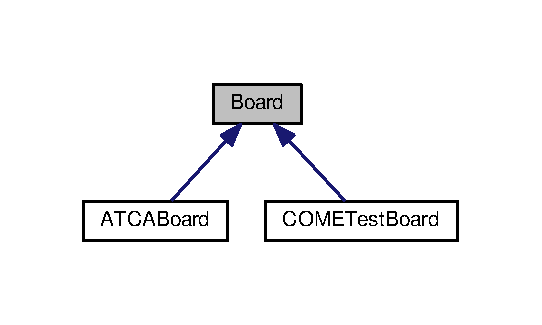
\includegraphics[width=260pt]{class_board__inherit__graph}
\end{center}
\end{figure}


Collaboration diagram for Board\+:\nopagebreak
\begin{figure}[H]
\begin{center}
\leavevmode
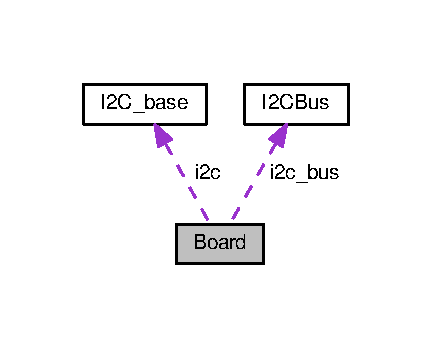
\includegraphics[width=208pt]{class_board__coll__graph}
\end{center}
\end{figure}
\subsection*{Public Member Functions}
\begin{DoxyCompactItemize}
\item 
virtual std\+::unordered\+\_\+map$<$ std\+::string, \hyperlink{class_i2_c_bus}{I2\+C\+Bus} $\ast$ $>$ \hyperlink{class_board_a7579517a69f81e2fcbe9e18857a11545}{get\+Map} (void)=0
\item 
void \hyperlink{class_board_ad01549e4fcb3d0dc2b7cab87b5d9be25}{set\+Bus} (std\+::string bus)
\begin{DoxyCompactList}\small\item\em Set bus to communicate over. \end{DoxyCompactList}\item 
void \hyperlink{class_board_aaa814c65e74c34a23deca4957b9c3e1c}{set\+Device} (std\+::string device)
\begin{DoxyCompactList}\small\item\em Set device to communicate to. \end{DoxyCompactList}\item 
void \hyperlink{class_board_ad6a4e4dec1a4be94b2eeb901e70fe710}{set\+Device} (std\+::string bus, std\+::string device)
\begin{DoxyCompactList}\small\item\em Set device to communicate to. \end{DoxyCompactList}\item 
void \hyperlink{class_board_ad8b29f72cded4b6a994b1999e91d7062}{set\+I2\+C\+Type} (\hyperlink{class_i2_c__base}{I2\+C\+\_\+base} $\ast$i2c\+\_\+type)
\begin{DoxyCompactList}\small\item\em Set I2C protocol. \end{DoxyCompactList}\item 
std\+::vector$<$ std\+::string $>$ \hyperlink{class_board_aa386db986f8d8865c3def1a941c79e2c}{get\+Buses} (void)
\begin{DoxyCompactList}\small\item\em Get available buses on board. \end{DoxyCompactList}\item 
std\+::vector$<$ std\+::string $>$ \hyperlink{class_board_a0be69177a3d368f3d02286d7114684cf}{get\+Devices} (void)
\begin{DoxyCompactList}\small\item\em Get available devices on selected bus. \end{DoxyCompactList}\item 
std\+::vector$<$ std\+::string $>$ \hyperlink{class_board_ab137346e2910c2e18b5bfb31b958c43b}{get\+Devices} (std\+::string bus)
\begin{DoxyCompactList}\small\item\em Get available devices on bus. \end{DoxyCompactList}\item 
std\+::vector$<$ std\+::string $>$ \hyperlink{class_board_a6f3cc9b5301912690da4e0eb939b3081}{get\+Properties} (void)
\begin{DoxyCompactList}\small\item\em Get available properties for selected device. \end{DoxyCompactList}\item 
std\+::vector$<$ std\+::string $>$ \hyperlink{class_board_a1fab797a0fbec9d42b3462cb24488e8a}{get\+Properties} (std\+::string device)
\begin{DoxyCompactList}\small\item\em Get available properties for device. \end{DoxyCompactList}\item 
std\+::vector$<$ std\+::string $>$ \hyperlink{class_board_a6ddcad5c21427323e5062bd22feba405}{get\+Properties} (std\+::string bus, std\+::string device)
\begin{DoxyCompactList}\small\item\em Get available properties for selected device. \end{DoxyCompactList}\item 
std\+::string \hyperlink{class_board_a0b500bd590d15f797d1a36ecfeb0f5d4}{read} (std\+::string property)
\begin{DoxyCompactList}\small\item\em Read value of property. \end{DoxyCompactList}\item 
void \hyperlink{class_board_ab99bb344ee68485ab89e1ed5b9d79d4e}{write} (std\+::string property, std\+::string value)
\begin{DoxyCompactList}\small\item\em Write value to property. \end{DoxyCompactList}\item 
\hyperlink{class_board_af90e83a4779ac782ff5cf22957bfae05}{Board} (int id)
\item 
\hyperlink{class_board_a737c0ecdabeccd0460bcbae2f8ac6c44}{$\sim$\+Board} (void)
\item 
const int \hyperlink{class_board_ab55397409307355c61edca9cb4c5236c}{get\+ID} (void) const 
\end{DoxyCompactItemize}
\subsection*{Public Attributes}
\begin{DoxyCompactItemize}
\item 
int \hyperlink{class_board_ac537a3646d93996bcf1c0ead77cf4ab5}{ID}
\end{DoxyCompactItemize}
\subsection*{Protected Attributes}
\begin{DoxyCompactItemize}
\item 
std\+::unordered\+\_\+map$<$ std\+::string, \hyperlink{class_i2_c_bus}{I2\+C\+Bus} $\ast$ $>$ \hyperlink{class_board_ac5fa25970ad12aa7d2c710bbcdd05339}{bus\+\_\+map}
\item 
\hyperlink{class_i2_c_bus}{I2\+C\+Bus} $\ast$ \hyperlink{class_board_a4458164bae62e6ba213a08a767242f9f}{i2c\+\_\+bus}
\item 
\hyperlink{class_i2_c__base}{I2\+C\+\_\+base} $\ast$ \hyperlink{class_board_aec7b3a540a138062fc54587e1040d917}{i2c}
\end{DoxyCompactItemize}


\subsection{Detailed Description}


Definition at line 34 of file Board.\+hpp.



\subsection{Constructor \& Destructor Documentation}
\index{Board@{Board}!Board@{Board}}
\index{Board@{Board}!Board@{Board}}
\subsubsection[{\texorpdfstring{Board(int id)}{Board(int id)}}]{\setlength{\rightskip}{0pt plus 5cm}Board\+::\+Board (
\begin{DoxyParamCaption}
\item[{int}]{id}
\end{DoxyParamCaption}
)\hspace{0.3cm}{\ttfamily [inline]}}\hypertarget{class_board_af90e83a4779ac782ff5cf22957bfae05}{}\label{class_board_af90e83a4779ac782ff5cf22957bfae05}


Definition at line 6 of file example.\+cpp.

\index{Board@{Board}!````~Board@{$\sim$\+Board}}
\index{````~Board@{$\sim$\+Board}!Board@{Board}}
\subsubsection[{\texorpdfstring{$\sim$\+Board(void)}{~Board(void)}}]{\setlength{\rightskip}{0pt plus 5cm}Board\+::$\sim$\+Board (
\begin{DoxyParamCaption}
\item[{void}]{}
\end{DoxyParamCaption}
)\hspace{0.3cm}{\ttfamily [inline]}}\hypertarget{class_board_a737c0ecdabeccd0460bcbae2f8ac6c44}{}\label{class_board_a737c0ecdabeccd0460bcbae2f8ac6c44}


Definition at line 9 of file example.\+cpp.



\subsection{Member Function Documentation}
\index{Board@{Board}!get\+Buses@{get\+Buses}}
\index{get\+Buses@{get\+Buses}!Board@{Board}}
\subsubsection[{\texorpdfstring{get\+Buses(void)}{getBuses(void)}}]{\setlength{\rightskip}{0pt plus 5cm}std\+::vector$<$ std\+::string $>$ Board\+::get\+Buses (
\begin{DoxyParamCaption}
\item[{void}]{}
\end{DoxyParamCaption}
)}\hypertarget{class_board_aa386db986f8d8865c3def1a941c79e2c}{}\label{class_board_aa386db986f8d8865c3def1a941c79e2c}


Get available buses on board. 

\begin{DoxyReturn}{Returns}
Vector of string I\+Ds for available buses. 
\end{DoxyReturn}


Definition at line 48 of file Board.\+cpp.

\index{Board@{Board}!get\+Devices@{get\+Devices}}
\index{get\+Devices@{get\+Devices}!Board@{Board}}
\subsubsection[{\texorpdfstring{get\+Devices(void)}{getDevices(void)}}]{\setlength{\rightskip}{0pt plus 5cm}std\+::vector$<$ std\+::string $>$ Board\+::get\+Devices (
\begin{DoxyParamCaption}
\item[{void}]{}
\end{DoxyParamCaption}
)}\hypertarget{class_board_a0be69177a3d368f3d02286d7114684cf}{}\label{class_board_a0be69177a3d368f3d02286d7114684cf}


Get available devices on selected bus. 

\begin{DoxyReturn}{Returns}
Vector of string I\+Ds for available devices. 
\end{DoxyReturn}


Definition at line 61 of file Board.\+cpp.

\index{Board@{Board}!get\+Devices@{get\+Devices}}
\index{get\+Devices@{get\+Devices}!Board@{Board}}
\subsubsection[{\texorpdfstring{get\+Devices(std\+::string bus)}{getDevices(std::string bus)}}]{\setlength{\rightskip}{0pt plus 5cm}std\+::vector$<$ std\+::string $>$ Board\+::get\+Devices (
\begin{DoxyParamCaption}
\item[{std\+::string}]{bus}
\end{DoxyParamCaption}
)}\hypertarget{class_board_ab137346e2910c2e18b5bfb31b958c43b}{}\label{class_board_ab137346e2910c2e18b5bfb31b958c43b}


Get available devices on bus. 


\begin{DoxyParams}{Parameters}
{\em bus} & -\/ String identifier for bus. \\
\hline
\end{DoxyParams}
\begin{DoxyReturn}{Returns}
Vector of string I\+Ds for available devices. 
\end{DoxyReturn}


Definition at line 70 of file Board.\+cpp.

\index{Board@{Board}!get\+ID@{get\+ID}}
\index{get\+ID@{get\+ID}!Board@{Board}}
\subsubsection[{\texorpdfstring{get\+I\+D(void) const }{getID(void) const }}]{\setlength{\rightskip}{0pt plus 5cm}const int Board\+::get\+ID (
\begin{DoxyParamCaption}
\item[{void}]{}
\end{DoxyParamCaption}
) const\hspace{0.3cm}{\ttfamily [inline]}}\hypertarget{class_board_ab55397409307355c61edca9cb4c5236c}{}\label{class_board_ab55397409307355c61edca9cb4c5236c}


Definition at line 10 of file example.\+cpp.

\index{Board@{Board}!get\+Map@{get\+Map}}
\index{get\+Map@{get\+Map}!Board@{Board}}
\subsubsection[{\texorpdfstring{get\+Map(void)=0}{getMap(void)=0}}]{\setlength{\rightskip}{0pt plus 5cm}virtual std\+::unordered\+\_\+map$<$std\+::string, {\bf I2\+C\+Bus}$\ast$$>$ Board\+::get\+Map (
\begin{DoxyParamCaption}
\item[{void}]{}
\end{DoxyParamCaption}
)\hspace{0.3cm}{\ttfamily [pure virtual]}}\hypertarget{class_board_a7579517a69f81e2fcbe9e18857a11545}{}\label{class_board_a7579517a69f81e2fcbe9e18857a11545}


Implemented in \hyperlink{class_a_t_c_a_board_a3926d4c4f9e4b98640b9b902b88ecb22}{A\+T\+C\+A\+Board}, and \hyperlink{class_c_o_m_e_test_board_ac8eff50bf63fbc98650b17579c858d73}{C\+O\+M\+E\+Test\+Board}.

\index{Board@{Board}!get\+Properties@{get\+Properties}}
\index{get\+Properties@{get\+Properties}!Board@{Board}}
\subsubsection[{\texorpdfstring{get\+Properties(void)}{getProperties(void)}}]{\setlength{\rightskip}{0pt plus 5cm}std\+::vector$<$ std\+::string $>$ Board\+::get\+Properties (
\begin{DoxyParamCaption}
\item[{void}]{}
\end{DoxyParamCaption}
)}\hypertarget{class_board_a6f3cc9b5301912690da4e0eb939b3081}{}\label{class_board_a6f3cc9b5301912690da4e0eb939b3081}


Get available properties for selected device. 

\begin{DoxyReturn}{Returns}
Vector of strings for each available property. 
\end{DoxyReturn}


Definition at line 79 of file Board.\+cpp.

\index{Board@{Board}!get\+Properties@{get\+Properties}}
\index{get\+Properties@{get\+Properties}!Board@{Board}}
\subsubsection[{\texorpdfstring{get\+Properties(std\+::string device)}{getProperties(std::string device)}}]{\setlength{\rightskip}{0pt plus 5cm}std\+::vector$<$ std\+::string $>$ Board\+::get\+Properties (
\begin{DoxyParamCaption}
\item[{std\+::string}]{device}
\end{DoxyParamCaption}
)}\hypertarget{class_board_a1fab797a0fbec9d42b3462cb24488e8a}{}\label{class_board_a1fab797a0fbec9d42b3462cb24488e8a}


Get available properties for device. 


\begin{DoxyParams}{Parameters}
{\em device} & -\/ String identifier for device. \\
\hline
\end{DoxyParams}
\begin{DoxyReturn}{Returns}
Vector of strings for each available property. 
\end{DoxyReturn}


Definition at line 88 of file Board.\+cpp.

\index{Board@{Board}!get\+Properties@{get\+Properties}}
\index{get\+Properties@{get\+Properties}!Board@{Board}}
\subsubsection[{\texorpdfstring{get\+Properties(std\+::string bus, std\+::string device)}{getProperties(std::string bus, std::string device)}}]{\setlength{\rightskip}{0pt plus 5cm}std\+::vector$<$ std\+::string $>$ Board\+::get\+Properties (
\begin{DoxyParamCaption}
\item[{std\+::string}]{bus, }
\item[{std\+::string}]{device}
\end{DoxyParamCaption}
)}\hypertarget{class_board_a6ddcad5c21427323e5062bd22feba405}{}\label{class_board_a6ddcad5c21427323e5062bd22feba405}


Get available properties for selected device. 


\begin{DoxyParams}{Parameters}
{\em bus} & -\/ String identifier for bus. \\
\hline
{\em device} & -\/ String identifier for device. \\
\hline
\end{DoxyParams}
\begin{DoxyReturn}{Returns}
Vector of strings for each available property. 
\end{DoxyReturn}


Definition at line 98 of file Board.\+cpp.

\index{Board@{Board}!read@{read}}
\index{read@{read}!Board@{Board}}
\subsubsection[{\texorpdfstring{read(std\+::string property)}{read(std::string property)}}]{\setlength{\rightskip}{0pt plus 5cm}std\+::string Board\+::read (
\begin{DoxyParamCaption}
\item[{std\+::string}]{property}
\end{DoxyParamCaption}
)}\hypertarget{class_board_a0b500bd590d15f797d1a36ecfeb0f5d4}{}\label{class_board_a0b500bd590d15f797d1a36ecfeb0f5d4}


Read value of property. 


\begin{DoxyParams}{Parameters}
{\em property} & -\/ String identifier for property. \\
\hline
\end{DoxyParams}
\begin{DoxyReturn}{Returns}
String of value and assosciated unit. 
\end{DoxyReturn}


Definition at line 108 of file Board.\+cpp.

\index{Board@{Board}!set\+Bus@{set\+Bus}}
\index{set\+Bus@{set\+Bus}!Board@{Board}}
\subsubsection[{\texorpdfstring{set\+Bus(std\+::string bus)}{setBus(std::string bus)}}]{\setlength{\rightskip}{0pt plus 5cm}void Board\+::set\+Bus (
\begin{DoxyParamCaption}
\item[{std\+::string}]{bus}
\end{DoxyParamCaption}
)}\hypertarget{class_board_ad01549e4fcb3d0dc2b7cab87b5d9be25}{}\label{class_board_ad01549e4fcb3d0dc2b7cab87b5d9be25}


Set bus to communicate over. 


\begin{DoxyParams}{Parameters}
{\em bus} & -\/ String identifier for bus. \\
\hline
\end{DoxyParams}


Definition at line 14 of file Board.\+cpp.

\index{Board@{Board}!set\+Device@{set\+Device}}
\index{set\+Device@{set\+Device}!Board@{Board}}
\subsubsection[{\texorpdfstring{set\+Device(std\+::string device)}{setDevice(std::string device)}}]{\setlength{\rightskip}{0pt plus 5cm}void Board\+::set\+Device (
\begin{DoxyParamCaption}
\item[{std\+::string}]{device}
\end{DoxyParamCaption}
)}\hypertarget{class_board_aaa814c65e74c34a23deca4957b9c3e1c}{}\label{class_board_aaa814c65e74c34a23deca4957b9c3e1c}


Set device to communicate to. 


\begin{DoxyParams}{Parameters}
{\em device} & -\/ String identifier for device. \\
\hline
\end{DoxyParams}


Definition at line 22 of file Board.\+cpp.

\index{Board@{Board}!set\+Device@{set\+Device}}
\index{set\+Device@{set\+Device}!Board@{Board}}
\subsubsection[{\texorpdfstring{set\+Device(std\+::string bus, std\+::string device)}{setDevice(std::string bus, std::string device)}}]{\setlength{\rightskip}{0pt plus 5cm}void Board\+::set\+Device (
\begin{DoxyParamCaption}
\item[{std\+::string}]{bus, }
\item[{std\+::string}]{device}
\end{DoxyParamCaption}
)}\hypertarget{class_board_ad6a4e4dec1a4be94b2eeb901e70fe710}{}\label{class_board_ad6a4e4dec1a4be94b2eeb901e70fe710}


Set device to communicate to. 


\begin{DoxyParams}{Parameters}
{\em bus} & -\/ String identifier for bus. \\
\hline
{\em device} & -\/ String identifier for device. \\
\hline
\end{DoxyParams}


Definition at line 31 of file Board.\+cpp.

\index{Board@{Board}!set\+I2\+C\+Type@{set\+I2\+C\+Type}}
\index{set\+I2\+C\+Type@{set\+I2\+C\+Type}!Board@{Board}}
\subsubsection[{\texorpdfstring{set\+I2\+C\+Type(\+I2\+C\+\_\+base $\ast$i2c\+\_\+type)}{setI2CType(I2C_base *i2c_type)}}]{\setlength{\rightskip}{0pt plus 5cm}void Board\+::set\+I2\+C\+Type (
\begin{DoxyParamCaption}
\item[{{\bf I2\+C\+\_\+base} $\ast$}]{i2c\+\_\+type}
\end{DoxyParamCaption}
)}\hypertarget{class_board_ad8b29f72cded4b6a994b1999e91d7062}{}\label{class_board_ad8b29f72cded4b6a994b1999e91d7062}


Set I2C protocol. 


\begin{DoxyParams}{Parameters}
{\em i2c\+\_\+type} & -\/ Pointer to \hyperlink{class_i2_c__base}{I2\+C\+\_\+base} object to be used for I2C communication. \\
\hline
\end{DoxyParams}


Definition at line 40 of file Board.\+cpp.

\index{Board@{Board}!write@{write}}
\index{write@{write}!Board@{Board}}
\subsubsection[{\texorpdfstring{write(std\+::string property, std\+::string value)}{write(std::string property, std::string value)}}]{\setlength{\rightskip}{0pt plus 5cm}void Board\+::write (
\begin{DoxyParamCaption}
\item[{std\+::string}]{property, }
\item[{std\+::string}]{value}
\end{DoxyParamCaption}
)}\hypertarget{class_board_ab99bb344ee68485ab89e1ed5b9d79d4e}{}\label{class_board_ab99bb344ee68485ab89e1ed5b9d79d4e}


Write value to property. 


\begin{DoxyParams}{Parameters}
{\em property} & -\/ String identifier for property. \\
\hline
{\em value} & -\/ String of value and assosciated unit. \\
\hline
\end{DoxyParams}


Definition at line 120 of file Board.\+cpp.



\subsection{Member Data Documentation}
\index{Board@{Board}!bus\+\_\+map@{bus\+\_\+map}}
\index{bus\+\_\+map@{bus\+\_\+map}!Board@{Board}}
\subsubsection[{\texorpdfstring{bus\+\_\+map}{bus_map}}]{\setlength{\rightskip}{0pt plus 5cm}std\+::unordered\+\_\+map$<$std\+::string, {\bf I2\+C\+Bus}$\ast$$>$ Board\+::bus\+\_\+map\hspace{0.3cm}{\ttfamily [protected]}}\hypertarget{class_board_ac5fa25970ad12aa7d2c710bbcdd05339}{}\label{class_board_ac5fa25970ad12aa7d2c710bbcdd05339}


Definition at line 36 of file Board.\+hpp.

\index{Board@{Board}!i2c@{i2c}}
\index{i2c@{i2c}!Board@{Board}}
\subsubsection[{\texorpdfstring{i2c}{i2c}}]{\setlength{\rightskip}{0pt plus 5cm}{\bf I2\+C\+\_\+base}$\ast$ Board\+::i2c\hspace{0.3cm}{\ttfamily [protected]}}\hypertarget{class_board_aec7b3a540a138062fc54587e1040d917}{}\label{class_board_aec7b3a540a138062fc54587e1040d917}


Definition at line 38 of file Board.\+hpp.

\index{Board@{Board}!i2c\+\_\+bus@{i2c\+\_\+bus}}
\index{i2c\+\_\+bus@{i2c\+\_\+bus}!Board@{Board}}
\subsubsection[{\texorpdfstring{i2c\+\_\+bus}{i2c_bus}}]{\setlength{\rightskip}{0pt plus 5cm}{\bf I2\+C\+Bus}$\ast$ Board\+::i2c\+\_\+bus\hspace{0.3cm}{\ttfamily [protected]}}\hypertarget{class_board_a4458164bae62e6ba213a08a767242f9f}{}\label{class_board_a4458164bae62e6ba213a08a767242f9f}


Definition at line 37 of file Board.\+hpp.

\index{Board@{Board}!ID@{ID}}
\index{ID@{ID}!Board@{Board}}
\subsubsection[{\texorpdfstring{ID}{ID}}]{\setlength{\rightskip}{0pt plus 5cm}int Board\+::\+ID}\hypertarget{class_board_ac537a3646d93996bcf1c0ead77cf4ab5}{}\label{class_board_ac537a3646d93996bcf1c0ead77cf4ab5}


Definition at line 5 of file example.\+cpp.



The documentation for this class was generated from the following files\+:\begin{DoxyCompactItemize}
\item 
include/\hyperlink{_board_8hpp}{Board.\+hpp}\item 
test/python/\hyperlink{example_8cpp}{example.\+cpp}\item 
src/\hyperlink{_board_8cpp}{Board.\+cpp}\end{DoxyCompactItemize}

\hypertarget{classnlohmann_1_1detail_1_1cached__input__stream__adapter}{}\section{nlohmann\+:\+:detail\+:\+:cached\+\_\+input\+\_\+stream\+\_\+adapter$<$ Buffer\+Size $>$ Class Template Reference}
\label{classnlohmann_1_1detail_1_1cached__input__stream__adapter}\index{nlohmann\+::detail\+::cached\+\_\+input\+\_\+stream\+\_\+adapter$<$ Buffer\+Size $>$@{nlohmann\+::detail\+::cached\+\_\+input\+\_\+stream\+\_\+adapter$<$ Buffer\+Size $>$}}


input adapter for cached stream input  




{\ttfamily \#include $<$json.\+hpp$>$}



Inheritance diagram for nlohmann\+:\+:detail\+:\+:cached\+\_\+input\+\_\+stream\+\_\+adapter$<$ Buffer\+Size $>$\+:\nopagebreak
\begin{figure}[H]
\begin{center}
\leavevmode
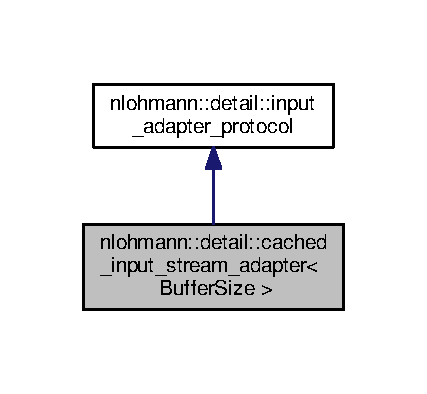
\includegraphics[width=205pt]{classnlohmann_1_1detail_1_1cached__input__stream__adapter__inherit__graph}
\end{center}
\end{figure}


Collaboration diagram for nlohmann\+:\+:detail\+:\+:cached\+\_\+input\+\_\+stream\+\_\+adapter$<$ Buffer\+Size $>$\+:\nopagebreak
\begin{figure}[H]
\begin{center}
\leavevmode
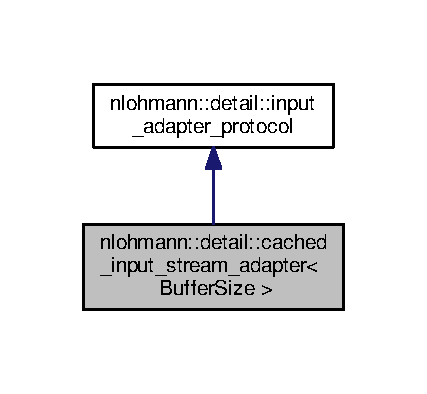
\includegraphics[width=205pt]{classnlohmann_1_1detail_1_1cached__input__stream__adapter__coll__graph}
\end{center}
\end{figure}
\subsection*{Public Member Functions}
\begin{DoxyCompactItemize}
\item 
\hyperlink{classnlohmann_1_1detail_1_1cached__input__stream__adapter_a4827c5bf63460dc04ce04d97d52d73b1}{cached\+\_\+input\+\_\+stream\+\_\+adapter} (std\+::istream \&i)
\item 
\hyperlink{classnlohmann_1_1detail_1_1cached__input__stream__adapter_a81ed6a4a86aee8d2cdb21a84a62744bb}{$\sim$cached\+\_\+input\+\_\+stream\+\_\+adapter} () override
\item 
int \hyperlink{classnlohmann_1_1detail_1_1cached__input__stream__adapter_a4a6fc864751cf727b134f1c2bf31b523}{get\+\_\+character} () override
\item 
\hyperlink{namespacenlohmann_1_1detail_a90aa5ef615aa8305e9ea20d8a947980fab45cffe084dd3d20d928bee85e7b0f21}{std\+::string} \hyperlink{classnlohmann_1_1detail_1_1cached__input__stream__adapter_ab9531a66a29685ec87646e99b516c263}{read} (std\+::size\+\_\+t offset, std\+::size\+\_\+t length) override
\end{DoxyCompactItemize}


\subsection{Detailed Description}
\subsubsection*{template$<$std\+::size\+\_\+t Buffer\+Size$>$\\*
class nlohmann\+::detail\+::cached\+\_\+input\+\_\+stream\+\_\+adapter$<$ Buffer\+Size $>$}

input adapter for cached stream input 

Definition at line 1306 of file json.\+hpp.



\subsection{Constructor \& Destructor Documentation}
\index{nlohmann\+::detail\+::cached\+\_\+input\+\_\+stream\+\_\+adapter@{nlohmann\+::detail\+::cached\+\_\+input\+\_\+stream\+\_\+adapter}!cached\+\_\+input\+\_\+stream\+\_\+adapter@{cached\+\_\+input\+\_\+stream\+\_\+adapter}}
\index{cached\+\_\+input\+\_\+stream\+\_\+adapter@{cached\+\_\+input\+\_\+stream\+\_\+adapter}!nlohmann\+::detail\+::cached\+\_\+input\+\_\+stream\+\_\+adapter@{nlohmann\+::detail\+::cached\+\_\+input\+\_\+stream\+\_\+adapter}}
\subsubsection[{\texorpdfstring{cached\+\_\+input\+\_\+stream\+\_\+adapter(std\+::istream \&i)}{cached_input_stream_adapter(std::istream &i)}}]{\setlength{\rightskip}{0pt plus 5cm}template$<$std\+::size\+\_\+t Buffer\+Size$>$ {\bf nlohmann\+::detail\+::cached\+\_\+input\+\_\+stream\+\_\+adapter}$<$ Buffer\+Size $>$\+::{\bf cached\+\_\+input\+\_\+stream\+\_\+adapter} (
\begin{DoxyParamCaption}
\item[{std\+::istream \&}]{i}
\end{DoxyParamCaption}
)\hspace{0.3cm}{\ttfamily [inline]}, {\ttfamily [explicit]}}\hypertarget{classnlohmann_1_1detail_1_1cached__input__stream__adapter_a4827c5bf63460dc04ce04d97d52d73b1}{}\label{classnlohmann_1_1detail_1_1cached__input__stream__adapter_a4827c5bf63460dc04ce04d97d52d73b1}


Definition at line 1309 of file json.\+hpp.

\index{nlohmann\+::detail\+::cached\+\_\+input\+\_\+stream\+\_\+adapter@{nlohmann\+::detail\+::cached\+\_\+input\+\_\+stream\+\_\+adapter}!````~cached\+\_\+input\+\_\+stream\+\_\+adapter@{$\sim$cached\+\_\+input\+\_\+stream\+\_\+adapter}}
\index{````~cached\+\_\+input\+\_\+stream\+\_\+adapter@{$\sim$cached\+\_\+input\+\_\+stream\+\_\+adapter}!nlohmann\+::detail\+::cached\+\_\+input\+\_\+stream\+\_\+adapter@{nlohmann\+::detail\+::cached\+\_\+input\+\_\+stream\+\_\+adapter}}
\subsubsection[{\texorpdfstring{$\sim$cached\+\_\+input\+\_\+stream\+\_\+adapter() override}{~cached_input_stream_adapter() override}}]{\setlength{\rightskip}{0pt plus 5cm}template$<$std\+::size\+\_\+t Buffer\+Size$>$ {\bf nlohmann\+::detail\+::cached\+\_\+input\+\_\+stream\+\_\+adapter}$<$ Buffer\+Size $>$\+::$\sim${\bf cached\+\_\+input\+\_\+stream\+\_\+adapter} (
\begin{DoxyParamCaption}
{}
\end{DoxyParamCaption}
)\hspace{0.3cm}{\ttfamily [inline]}, {\ttfamily [override]}}\hypertarget{classnlohmann_1_1detail_1_1cached__input__stream__adapter_a81ed6a4a86aee8d2cdb21a84a62744bb}{}\label{classnlohmann_1_1detail_1_1cached__input__stream__adapter_a81ed6a4a86aee8d2cdb21a84a62744bb}


Definition at line 1322 of file json.\+hpp.



\subsection{Member Function Documentation}
\index{nlohmann\+::detail\+::cached\+\_\+input\+\_\+stream\+\_\+adapter@{nlohmann\+::detail\+::cached\+\_\+input\+\_\+stream\+\_\+adapter}!get\+\_\+character@{get\+\_\+character}}
\index{get\+\_\+character@{get\+\_\+character}!nlohmann\+::detail\+::cached\+\_\+input\+\_\+stream\+\_\+adapter@{nlohmann\+::detail\+::cached\+\_\+input\+\_\+stream\+\_\+adapter}}
\subsubsection[{\texorpdfstring{get\+\_\+character() override}{get_character() override}}]{\setlength{\rightskip}{0pt plus 5cm}template$<$std\+::size\+\_\+t Buffer\+Size$>$ int {\bf nlohmann\+::detail\+::cached\+\_\+input\+\_\+stream\+\_\+adapter}$<$ Buffer\+Size $>$\+::get\+\_\+character (
\begin{DoxyParamCaption}
{}
\end{DoxyParamCaption}
)\hspace{0.3cm}{\ttfamily [inline]}, {\ttfamily [override]}, {\ttfamily [virtual]}}\hypertarget{classnlohmann_1_1detail_1_1cached__input__stream__adapter_a4a6fc864751cf727b134f1c2bf31b523}{}\label{classnlohmann_1_1detail_1_1cached__input__stream__adapter_a4a6fc864751cf727b134f1c2bf31b523}


Implements \hyperlink{structnlohmann_1_1detail_1_1input__adapter__protocol_af4e0baade0a6b45a73d4e136875e7544}{nlohmann\+::detail\+::input\+\_\+adapter\+\_\+protocol}.



Definition at line 1335 of file json.\+hpp.

\index{nlohmann\+::detail\+::cached\+\_\+input\+\_\+stream\+\_\+adapter@{nlohmann\+::detail\+::cached\+\_\+input\+\_\+stream\+\_\+adapter}!read@{read}}
\index{read@{read}!nlohmann\+::detail\+::cached\+\_\+input\+\_\+stream\+\_\+adapter@{nlohmann\+::detail\+::cached\+\_\+input\+\_\+stream\+\_\+adapter}}
\subsubsection[{\texorpdfstring{read(std\+::size\+\_\+t offset, std\+::size\+\_\+t length) override}{read(std::size_t offset, std::size_t length) override}}]{\setlength{\rightskip}{0pt plus 5cm}template$<$std\+::size\+\_\+t Buffer\+Size$>$ {\bf std\+::string} {\bf nlohmann\+::detail\+::cached\+\_\+input\+\_\+stream\+\_\+adapter}$<$ Buffer\+Size $>$\+::read (
\begin{DoxyParamCaption}
\item[{std\+::size\+\_\+t}]{offset, }
\item[{std\+::size\+\_\+t}]{length}
\end{DoxyParamCaption}
)\hspace{0.3cm}{\ttfamily [inline]}, {\ttfamily [override]}, {\ttfamily [virtual]}}\hypertarget{classnlohmann_1_1detail_1_1cached__input__stream__adapter_ab9531a66a29685ec87646e99b516c263}{}\label{classnlohmann_1_1detail_1_1cached__input__stream__adapter_ab9531a66a29685ec87646e99b516c263}


Implements \hyperlink{structnlohmann_1_1detail_1_1input__adapter__protocol_a9ce6c8028229446d7014c0610fbd4599}{nlohmann\+::detail\+::input\+\_\+adapter\+\_\+protocol}.



Definition at line 1358 of file json.\+hpp.



The documentation for this class was generated from the following file\+:\begin{DoxyCompactItemize}
\item 
include/\hyperlink{json_8hpp}{json.\+hpp}\end{DoxyCompactItemize}

\hypertarget{class_client}{}\section{Client Class Reference}
\label{class_client}\index{Client@{Client}}


{\ttfamily \#include $<$Couch\+D\+B.\+hpp$>$}



Inheritance diagram for Client\+:\nopagebreak
\begin{figure}[H]
\begin{center}
\leavevmode
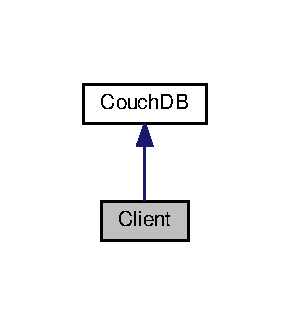
\includegraphics[width=139pt]{class_client__inherit__graph}
\end{center}
\end{figure}


Collaboration diagram for Client\+:\nopagebreak
\begin{figure}[H]
\begin{center}
\leavevmode
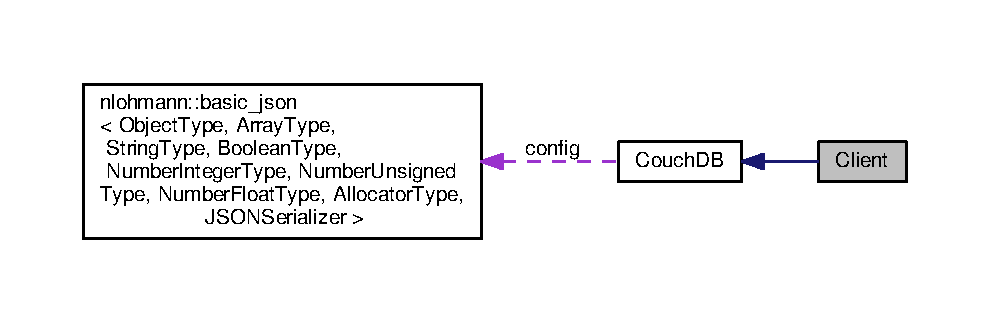
\includegraphics[width=350pt]{class_client__coll__graph}
\end{center}
\end{figure}
\subsection*{Public Member Functions}
\begin{DoxyCompactItemize}
\item 
\hyperlink{class_client_adc081e1006b31b0e5ded80c71e3ada70}{Client} (void)
\begin{DoxyCompactList}\small\item\em Class constructor. \end{DoxyCompactList}\item 
\hyperlink{class_client_a8e19879cb7c39c111b523ed216273203}{Client} (std\+::string url\+\_\+)
\begin{DoxyCompactList}\small\item\em Class constructor. \end{DoxyCompactList}\item 
\hyperlink{class_client_a66e3074e5f09c5e9bb4ec36bdea01c91}{$\sim$\+Client} (void)
\begin{DoxyCompactList}\small\item\em Class destructor. \end{DoxyCompactList}\item 
std\+::vector$<$ std\+::string $>$ \hyperlink{class_client_a19ad3503375f64a4b68e20dbc98703c4}{get\+Databases} (void)
\begin{DoxyCompactList}\small\item\em Get list of databases on server. \end{DoxyCompactList}\item 
void \hyperlink{class_client_a6481994d5e2711bf43bca04460cb2316}{set\+Database} (std\+::string db)
\begin{DoxyCompactList}\small\item\em Set ID of database to work with. \end{DoxyCompactList}\item 
void \hyperlink{class_client_ae9c82ded3834b156fb98e16bdac2a05f}{upload\+Document} (\hyperlink{_couch_d_b_8hpp_ab701e3ac61a85b337ec5c1abaad6742d}{json} data)
\begin{DoxyCompactList}\small\item\em Upload document to database. \end{DoxyCompactList}\item 
void \hyperlink{class_client_ad6e6281bbd3cba141664bf2c0ac87227}{upload\+Document} (std\+::string url\+\_\+, \hyperlink{_couch_d_b_8hpp_ab701e3ac61a85b337ec5c1abaad6742d}{json} data)
\begin{DoxyCompactList}\small\item\em Upload document to database. \end{DoxyCompactList}\item 
void \hyperlink{class_client_a4983d1069b46cbb8926f9094853936c1}{push\+Database} (void)
\begin{DoxyCompactList}\small\item\em Replicate database to master server. \end{DoxyCompactList}\item 
void \hyperlink{class_client_a3ff5f11c6665c7b9c99476d158b02c01}{push\+Database} (\hyperlink{_couch_d_b_8hpp_ab701e3ac61a85b337ec5c1abaad6742d}{json} params)
\begin{DoxyCompactList}\small\item\em Replicate database to master server with specific parameters. \end{DoxyCompactList}\item 
std\+::string \hyperlink{class_client_a8f8ca876b5bc3b75cf642e5de8c25b20}{get\+Document} (std\+::string doc)
\begin{DoxyCompactList}\small\item\em Upload document to database. \end{DoxyCompactList}\item 
std\+::vector$<$ std\+::pair$<$ std\+::string, std\+::string $>$ $>$ \hyperlink{class_client_ad24ac9ee317e61cf04a565c4e849f31c}{get\+Document\+I\+Ds} (void)
\begin{DoxyCompactList}\small\item\em Get document I\+Ds and revision I\+Ds for given database. \end{DoxyCompactList}\item 
bool \hyperlink{class_client_ae504f5c93e2783a4ebb26ee94a002327}{check\+Online} (std\+::string url\+\_\+)
\begin{DoxyCompactList}\small\item\em Check if server is online. \end{DoxyCompactList}\item 
void \hyperlink{class_client_a45748961b6b8b534fa04e9a2bb40ed27}{delete\+Document} (std\+::string ID, std\+::string rev)
\begin{DoxyCompactList}\small\item\em Delete document from database. \end{DoxyCompactList}\item 
void \hyperlink{class_client_ab4703ff4ad0742e72c5416f33971cc2f}{compact\+Database} (void)
\end{DoxyCompactItemize}
\subsection*{Additional Inherited Members}


\subsection{Detailed Description}


Definition at line 32 of file Couch\+D\+B.\+hpp.



\subsection{Constructor \& Destructor Documentation}
\index{Client@{Client}!Client@{Client}}
\index{Client@{Client}!Client@{Client}}
\subsubsection[{\texorpdfstring{Client(void)}{Client(void)}}]{\setlength{\rightskip}{0pt plus 5cm}Client\+::\+Client (
\begin{DoxyParamCaption}
\item[{void}]{}
\end{DoxyParamCaption}
)}\hypertarget{class_client_adc081e1006b31b0e5ded80c71e3ada70}{}\label{class_client_adc081e1006b31b0e5ded80c71e3ada70}


Class constructor. 



Definition at line 117 of file Couch\+D\+B.\+cpp.

\index{Client@{Client}!Client@{Client}}
\index{Client@{Client}!Client@{Client}}
\subsubsection[{\texorpdfstring{Client(std\+::string url\+\_\+)}{Client(std::string url_)}}]{\setlength{\rightskip}{0pt plus 5cm}Client\+::\+Client (
\begin{DoxyParamCaption}
\item[{std\+::string}]{url\+\_\+}
\end{DoxyParamCaption}
)}\hypertarget{class_client_a8e19879cb7c39c111b523ed216273203}{}\label{class_client_a8e19879cb7c39c111b523ed216273203}


Class constructor. 


\begin{DoxyParams}{Parameters}
{\em url\+\_\+} & -\/ U\+RL of \hyperlink{class_couch_d_b}{Couch\+DB} server. \\
\hline
\end{DoxyParams}


Definition at line 127 of file Couch\+D\+B.\+cpp.

\index{Client@{Client}!````~Client@{$\sim$\+Client}}
\index{````~Client@{$\sim$\+Client}!Client@{Client}}
\subsubsection[{\texorpdfstring{$\sim$\+Client(void)}{~Client(void)}}]{\setlength{\rightskip}{0pt plus 5cm}Client\+::$\sim$\+Client (
\begin{DoxyParamCaption}
\item[{void}]{}
\end{DoxyParamCaption}
)}\hypertarget{class_client_a66e3074e5f09c5e9bb4ec36bdea01c91}{}\label{class_client_a66e3074e5f09c5e9bb4ec36bdea01c91}


Class destructor. 



Definition at line 136 of file Couch\+D\+B.\+cpp.



\subsection{Member Function Documentation}
\index{Client@{Client}!check\+Online@{check\+Online}}
\index{check\+Online@{check\+Online}!Client@{Client}}
\subsubsection[{\texorpdfstring{check\+Online(std\+::string url\+\_\+)}{checkOnline(std::string url_)}}]{\setlength{\rightskip}{0pt plus 5cm}bool Client\+::check\+Online (
\begin{DoxyParamCaption}
\item[{std\+::string}]{url\+\_\+}
\end{DoxyParamCaption}
)}\hypertarget{class_client_ae504f5c93e2783a4ebb26ee94a002327}{}\label{class_client_ae504f5c93e2783a4ebb26ee94a002327}


Check if server is online. 


\begin{DoxyParams}{Parameters}
{\em url\+\_\+} & -\/ U\+RL of server to check. \\
\hline
\end{DoxyParams}
\begin{DoxyReturn}{Returns}
True if online, throws error if not. T\+O\+DO make this so that it does not throw error? This is legacy from Python/bash. 
\end{DoxyReturn}


Definition at line 240 of file Couch\+D\+B.\+cpp.

\index{Client@{Client}!compact\+Database@{compact\+Database}}
\index{compact\+Database@{compact\+Database}!Client@{Client}}
\subsubsection[{\texorpdfstring{compact\+Database(void)}{compactDatabase(void)}}]{\setlength{\rightskip}{0pt plus 5cm}void Client\+::compact\+Database (
\begin{DoxyParamCaption}
\item[{void}]{}
\end{DoxyParamCaption}
)}\hypertarget{class_client_ab4703ff4ad0742e72c5416f33971cc2f}{}\label{class_client_ab4703ff4ad0742e72c5416f33971cc2f}
Compact database to save space on local machine. 

Definition at line 259 of file Couch\+D\+B.\+cpp.

\index{Client@{Client}!delete\+Document@{delete\+Document}}
\index{delete\+Document@{delete\+Document}!Client@{Client}}
\subsubsection[{\texorpdfstring{delete\+Document(std\+::string I\+D, std\+::string rev)}{deleteDocument(std::string ID, std::string rev)}}]{\setlength{\rightskip}{0pt plus 5cm}void Client\+::delete\+Document (
\begin{DoxyParamCaption}
\item[{std\+::string}]{ID, }
\item[{std\+::string}]{rev}
\end{DoxyParamCaption}
)}\hypertarget{class_client_a45748961b6b8b534fa04e9a2bb40ed27}{}\label{class_client_a45748961b6b8b534fa04e9a2bb40ed27}


Delete document from database. 


\begin{DoxyParams}{Parameters}
{\em ID} & -\/ ID of document. \\
\hline
{\em rev} & -\/ revision of document. \\
\hline
\end{DoxyParams}


Definition at line 251 of file Couch\+D\+B.\+cpp.

\index{Client@{Client}!get\+Databases@{get\+Databases}}
\index{get\+Databases@{get\+Databases}!Client@{Client}}
\subsubsection[{\texorpdfstring{get\+Databases(void)}{getDatabases(void)}}]{\setlength{\rightskip}{0pt plus 5cm}std\+::vector$<$ std\+::string $>$ Client\+::get\+Databases (
\begin{DoxyParamCaption}
\item[{void}]{}
\end{DoxyParamCaption}
)}\hypertarget{class_client_a19ad3503375f64a4b68e20dbc98703c4}{}\label{class_client_a19ad3503375f64a4b68e20dbc98703c4}


Get list of databases on server. 

\begin{DoxyReturn}{Returns}
Vector of strings of I\+Ds of each database. 
\end{DoxyReturn}


Definition at line 144 of file Couch\+D\+B.\+cpp.

\index{Client@{Client}!get\+Document@{get\+Document}}
\index{get\+Document@{get\+Document}!Client@{Client}}
\subsubsection[{\texorpdfstring{get\+Document(std\+::string doc)}{getDocument(std::string doc)}}]{\setlength{\rightskip}{0pt plus 5cm}std\+::string Client\+::get\+Document (
\begin{DoxyParamCaption}
\item[{std\+::string}]{doc}
\end{DoxyParamCaption}
)}\hypertarget{class_client_a8f8ca876b5bc3b75cf642e5de8c25b20}{}\label{class_client_a8f8ca876b5bc3b75cf642e5de8c25b20}


Upload document to database. 


\begin{DoxyParams}{Parameters}
{\em doc} & -\/ Document ID. \\
\hline
\end{DoxyParams}
\begin{DoxyReturn}{Returns}
String representation of J\+S\+ON output. 
\end{DoxyReturn}


Definition at line 214 of file Couch\+D\+B.\+cpp.

\index{Client@{Client}!get\+Document\+I\+Ds@{get\+Document\+I\+Ds}}
\index{get\+Document\+I\+Ds@{get\+Document\+I\+Ds}!Client@{Client}}
\subsubsection[{\texorpdfstring{get\+Document\+I\+Ds(void)}{getDocumentIDs(void)}}]{\setlength{\rightskip}{0pt plus 5cm}std\+::vector$<$ std\+::pair$<$ std\+::string, std\+::string $>$ $>$ Client\+::get\+Document\+I\+Ds (
\begin{DoxyParamCaption}
\item[{void}]{}
\end{DoxyParamCaption}
)}\hypertarget{class_client_ad24ac9ee317e61cf04a565c4e849f31c}{}\label{class_client_ad24ac9ee317e61cf04a565c4e849f31c}


Get document I\+Ds and revision I\+Ds for given database. 

\begin{DoxyReturn}{Returns}
Vector of string pairs for ID and revision. 
\end{DoxyReturn}


Definition at line 224 of file Couch\+D\+B.\+cpp.

\index{Client@{Client}!push\+Database@{push\+Database}}
\index{push\+Database@{push\+Database}!Client@{Client}}
\subsubsection[{\texorpdfstring{push\+Database(void)}{pushDatabase(void)}}]{\setlength{\rightskip}{0pt plus 5cm}void Client\+::push\+Database (
\begin{DoxyParamCaption}
\item[{void}]{}
\end{DoxyParamCaption}
)}\hypertarget{class_client_a4983d1069b46cbb8926f9094853936c1}{}\label{class_client_a4983d1069b46cbb8926f9094853936c1}


Replicate database to master server. 



Definition at line 190 of file Couch\+D\+B.\+cpp.

\index{Client@{Client}!push\+Database@{push\+Database}}
\index{push\+Database@{push\+Database}!Client@{Client}}
\subsubsection[{\texorpdfstring{push\+Database(json params)}{pushDatabase(json params)}}]{\setlength{\rightskip}{0pt plus 5cm}void Client\+::push\+Database (
\begin{DoxyParamCaption}
\item[{{\bf json}}]{params}
\end{DoxyParamCaption}
)}\hypertarget{class_client_a3ff5f11c6665c7b9c99476d158b02c01}{}\label{class_client_a3ff5f11c6665c7b9c99476d158b02c01}


Replicate database to master server with specific parameters. 


\begin{DoxyParams}{Parameters}
{\em params} & -\/ J\+S\+ON key-\/value pairs for filter function. \\
\hline
\end{DoxyParams}


Definition at line 201 of file Couch\+D\+B.\+cpp.

\index{Client@{Client}!set\+Database@{set\+Database}}
\index{set\+Database@{set\+Database}!Client@{Client}}
\subsubsection[{\texorpdfstring{set\+Database(std\+::string db)}{setDatabase(std::string db)}}]{\setlength{\rightskip}{0pt plus 5cm}void Client\+::set\+Database (
\begin{DoxyParamCaption}
\item[{std\+::string}]{db}
\end{DoxyParamCaption}
)}\hypertarget{class_client_a6481994d5e2711bf43bca04460cb2316}{}\label{class_client_a6481994d5e2711bf43bca04460cb2316}


Set ID of database to work with. 


\begin{DoxyParams}{Parameters}
{\em db} & -\/ Database ID. \\
\hline
\end{DoxyParams}


Definition at line 158 of file Couch\+D\+B.\+cpp.

\index{Client@{Client}!upload\+Document@{upload\+Document}}
\index{upload\+Document@{upload\+Document}!Client@{Client}}
\subsubsection[{\texorpdfstring{upload\+Document(json data)}{uploadDocument(json data)}}]{\setlength{\rightskip}{0pt plus 5cm}void Client\+::upload\+Document (
\begin{DoxyParamCaption}
\item[{{\bf json}}]{data}
\end{DoxyParamCaption}
)}\hypertarget{class_client_ae9c82ded3834b156fb98e16bdac2a05f}{}\label{class_client_ae9c82ded3834b156fb98e16bdac2a05f}


Upload document to database. 


\begin{DoxyParams}{Parameters}
{\em data} & -\/ J\+S\+ON table to upload. \\
\hline
\end{DoxyParams}


Definition at line 166 of file Couch\+D\+B.\+cpp.

\index{Client@{Client}!upload\+Document@{upload\+Document}}
\index{upload\+Document@{upload\+Document}!Client@{Client}}
\subsubsection[{\texorpdfstring{upload\+Document(std\+::string url\+\_\+, json data)}{uploadDocument(std::string url_, json data)}}]{\setlength{\rightskip}{0pt plus 5cm}void Client\+::upload\+Document (
\begin{DoxyParamCaption}
\item[{std\+::string}]{url\+\_\+, }
\item[{{\bf json}}]{data}
\end{DoxyParamCaption}
)}\hypertarget{class_client_ad6e6281bbd3cba141664bf2c0ac87227}{}\label{class_client_ad6e6281bbd3cba141664bf2c0ac87227}


Upload document to database. 


\begin{DoxyParams}{Parameters}
{\em url\+\_\+} & -\/ U\+RL of database to upload to. \\
\hline
{\em data} & -\/ J\+S\+ON table to upload. \\
\hline
\end{DoxyParams}


Definition at line 180 of file Couch\+D\+B.\+cpp.



The documentation for this class was generated from the following files\+:\begin{DoxyCompactItemize}
\item 
include/\hyperlink{_couch_d_b_8hpp}{Couch\+D\+B.\+hpp}\item 
src/\hyperlink{_couch_d_b_8cpp}{Couch\+D\+B.\+cpp}\end{DoxyCompactItemize}

\hypertarget{class_c_o_m_e_test_board}{}\section{C\+O\+M\+E\+Test\+Board Class Reference}
\label{class_c_o_m_e_test_board}\index{C\+O\+M\+E\+Test\+Board@{C\+O\+M\+E\+Test\+Board}}


{\ttfamily \#include $<$C\+O\+M\+E\+Test\+Board.\+hpp$>$}



Inheritance diagram for C\+O\+M\+E\+Test\+Board\+:\nopagebreak
\begin{figure}[H]
\begin{center}
\leavevmode
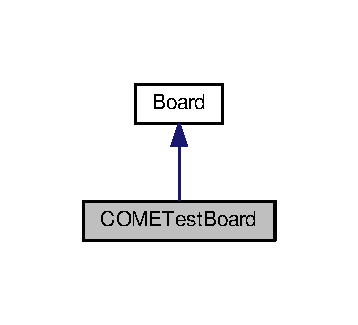
\includegraphics[width=172pt]{class_c_o_m_e_test_board__inherit__graph}
\end{center}
\end{figure}


Collaboration diagram for C\+O\+M\+E\+Test\+Board\+:\nopagebreak
\begin{figure}[H]
\begin{center}
\leavevmode
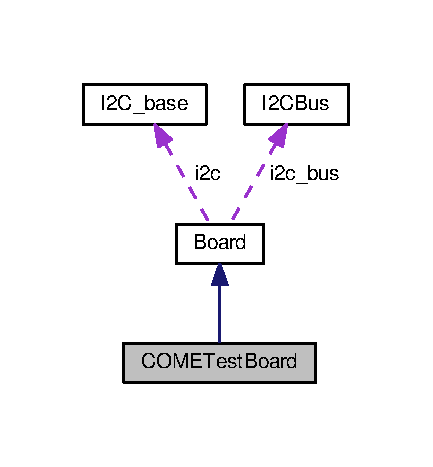
\includegraphics[width=208pt]{class_c_o_m_e_test_board__coll__graph}
\end{center}
\end{figure}
\subsection*{Public Member Functions}
\begin{DoxyCompactItemize}
\item 
\hyperlink{class_c_o_m_e_test_board_a373116ab895fdabcec6c73b193b925e7}{C\+O\+M\+E\+Test\+Board} (\hyperlink{class_i2_c__base}{I2\+C\+\_\+base} $\ast$i2c\+\_\+type)
\begin{DoxyCompactList}\small\item\em Class constructor. Full bus/device/register map is defined here. \end{DoxyCompactList}\item 
\hyperlink{class_c_o_m_e_test_board_ae4a09594e1ce42977dd71e48356e5136}{C\+O\+M\+E\+Test\+Board} (std\+::string i2c\+\_\+string)
\begin{DoxyCompactList}\small\item\em Class constructor. Full bus/device/register map is defined here. Also requests downstream bus from arbiter. \end{DoxyCompactList}\item 
\hyperlink{class_c_o_m_e_test_board_a6bacaca3d2bf5a32fa4881f9c06924db}{$\sim$\+C\+O\+M\+E\+Test\+Board} (void)
\begin{DoxyCompactList}\small\item\em Class destructor. Gives up downstream bus to arbiter. \end{DoxyCompactList}\item 
std\+::unordered\+\_\+map$<$ std\+::string, \hyperlink{class_i2_c_bus}{I2\+C\+Bus} $\ast$ $>$ \hyperlink{class_c_o_m_e_test_board_ac8eff50bf63fbc98650b17579c858d73}{get\+Map} (void)
\begin{DoxyCompactList}\small\item\em Get the map. \end{DoxyCompactList}\end{DoxyCompactItemize}
\subsection*{Additional Inherited Members}


\subsection{Detailed Description}


Definition at line 12 of file C\+O\+M\+E\+Test\+Board.\+hpp.



\subsection{Constructor \& Destructor Documentation}
\index{C\+O\+M\+E\+Test\+Board@{C\+O\+M\+E\+Test\+Board}!C\+O\+M\+E\+Test\+Board@{C\+O\+M\+E\+Test\+Board}}
\index{C\+O\+M\+E\+Test\+Board@{C\+O\+M\+E\+Test\+Board}!C\+O\+M\+E\+Test\+Board@{C\+O\+M\+E\+Test\+Board}}
\subsubsection[{\texorpdfstring{C\+O\+M\+E\+Test\+Board(\+I2\+C\+\_\+base $\ast$i2c\+\_\+type)}{COMETestBoard(I2C_base *i2c_type)}}]{\setlength{\rightskip}{0pt plus 5cm}C\+O\+M\+E\+Test\+Board\+::\+C\+O\+M\+E\+Test\+Board (
\begin{DoxyParamCaption}
\item[{{\bf I2\+C\+\_\+base} $\ast$}]{i2c\+\_\+type}
\end{DoxyParamCaption}
)}\hypertarget{class_c_o_m_e_test_board_a373116ab895fdabcec6c73b193b925e7}{}\label{class_c_o_m_e_test_board_a373116ab895fdabcec6c73b193b925e7}


Class constructor. Full bus/device/register map is defined here. 


\begin{DoxyParams}{Parameters}
{\em i2c\+\_\+type} & -\/ Pointer to I2C transport class to be used. \\
\hline
\end{DoxyParams}


Definition at line 15 of file C\+O\+M\+E\+Test\+Board.\+cpp.

\index{C\+O\+M\+E\+Test\+Board@{C\+O\+M\+E\+Test\+Board}!C\+O\+M\+E\+Test\+Board@{C\+O\+M\+E\+Test\+Board}}
\index{C\+O\+M\+E\+Test\+Board@{C\+O\+M\+E\+Test\+Board}!C\+O\+M\+E\+Test\+Board@{C\+O\+M\+E\+Test\+Board}}
\subsubsection[{\texorpdfstring{C\+O\+M\+E\+Test\+Board(std\+::string i2c\+\_\+string)}{COMETestBoard(std::string i2c_string)}}]{\setlength{\rightskip}{0pt plus 5cm}C\+O\+M\+E\+Test\+Board\+::\+C\+O\+M\+E\+Test\+Board (
\begin{DoxyParamCaption}
\item[{std\+::string}]{i2c\+\_\+string}
\end{DoxyParamCaption}
)}\hypertarget{class_c_o_m_e_test_board_ae4a09594e1ce42977dd71e48356e5136}{}\label{class_c_o_m_e_test_board_ae4a09594e1ce42977dd71e48356e5136}


Class constructor. Full bus/device/register map is defined here. Also requests downstream bus from arbiter. 


\begin{DoxyParams}{Parameters}
{\em i2c\+\_\+type} & -\/ Pointer to \hyperlink{class_i2_c__base}{I2\+C\+\_\+base} transport object. \\
\hline
\end{DoxyParams}


Definition at line 54 of file C\+O\+M\+E\+Test\+Board.\+cpp.

\index{C\+O\+M\+E\+Test\+Board@{C\+O\+M\+E\+Test\+Board}!````~C\+O\+M\+E\+Test\+Board@{$\sim$\+C\+O\+M\+E\+Test\+Board}}
\index{````~C\+O\+M\+E\+Test\+Board@{$\sim$\+C\+O\+M\+E\+Test\+Board}!C\+O\+M\+E\+Test\+Board@{C\+O\+M\+E\+Test\+Board}}
\subsubsection[{\texorpdfstring{$\sim$\+C\+O\+M\+E\+Test\+Board(void)}{~COMETestBoard(void)}}]{\setlength{\rightskip}{0pt plus 5cm}C\+O\+M\+E\+Test\+Board\+::$\sim$\+C\+O\+M\+E\+Test\+Board (
\begin{DoxyParamCaption}
\item[{void}]{}
\end{DoxyParamCaption}
)}\hypertarget{class_c_o_m_e_test_board_a6bacaca3d2bf5a32fa4881f9c06924db}{}\label{class_c_o_m_e_test_board_a6bacaca3d2bf5a32fa4881f9c06924db}


Class destructor. Gives up downstream bus to arbiter. 



Definition at line 97 of file C\+O\+M\+E\+Test\+Board.\+cpp.



\subsection{Member Function Documentation}
\index{C\+O\+M\+E\+Test\+Board@{C\+O\+M\+E\+Test\+Board}!get\+Map@{get\+Map}}
\index{get\+Map@{get\+Map}!C\+O\+M\+E\+Test\+Board@{C\+O\+M\+E\+Test\+Board}}
\subsubsection[{\texorpdfstring{get\+Map(void)}{getMap(void)}}]{\setlength{\rightskip}{0pt plus 5cm}std\+::unordered\+\_\+map$<$ std\+::string, {\bf I2\+C\+Bus} $\ast$ $>$ C\+O\+M\+E\+Test\+Board\+::get\+Map (
\begin{DoxyParamCaption}
\item[{void}]{}
\end{DoxyParamCaption}
)\hspace{0.3cm}{\ttfamily [virtual]}}\hypertarget{class_c_o_m_e_test_board_ac8eff50bf63fbc98650b17579c858d73}{}\label{class_c_o_m_e_test_board_ac8eff50bf63fbc98650b17579c858d73}


Get the map. 

\begin{DoxyReturn}{Returns}
Unordered map of string identifiers and \hyperlink{class_i2_c_bus}{I2\+C\+Bus} pointers. 
\end{DoxyReturn}


Implements \hyperlink{class_board_a7579517a69f81e2fcbe9e18857a11545}{Board}.



Definition at line 105 of file C\+O\+M\+E\+Test\+Board.\+cpp.



The documentation for this class was generated from the following files\+:\begin{DoxyCompactItemize}
\item 
include/\hyperlink{_c_o_m_e_test_board_8hpp}{C\+O\+M\+E\+Test\+Board.\+hpp}\item 
src/\hyperlink{_c_o_m_e_test_board_8cpp}{C\+O\+M\+E\+Test\+Board.\+cpp}\end{DoxyCompactItemize}

\hypertarget{structnlohmann_1_1detail_1_1conjunction}{}\section{nlohmann\+:\+:detail\+:\+:conjunction$<$... $>$ Struct Template Reference}
\label{structnlohmann_1_1detail_1_1conjunction}\index{nlohmann\+::detail\+::conjunction$<$... $>$@{nlohmann\+::detail\+::conjunction$<$... $>$}}


{\ttfamily \#include $<$json.\+hpp$>$}



Inheritance diagram for nlohmann\+:\+:detail\+:\+:conjunction$<$... $>$\+:\nopagebreak
\begin{figure}[H]
\begin{center}
\leavevmode
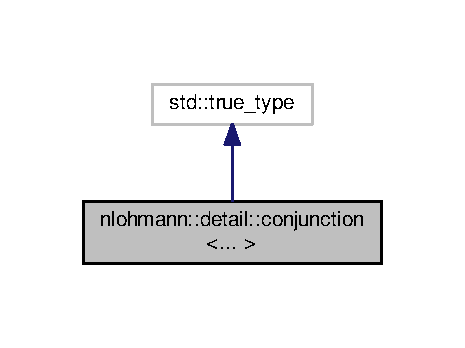
\includegraphics[width=223pt]{structnlohmann_1_1detail_1_1conjunction__inherit__graph}
\end{center}
\end{figure}


Collaboration diagram for nlohmann\+:\+:detail\+:\+:conjunction$<$... $>$\+:\nopagebreak
\begin{figure}[H]
\begin{center}
\leavevmode
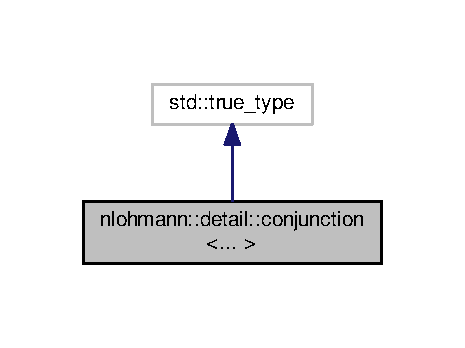
\includegraphics[width=223pt]{structnlohmann_1_1detail_1_1conjunction__coll__graph}
\end{center}
\end{figure}


\subsection{Detailed Description}
\subsubsection*{template$<$class...$>$\\*
struct nlohmann\+::detail\+::conjunction$<$... $>$}



Definition at line 538 of file json.\+hpp.



The documentation for this struct was generated from the following file\+:\begin{DoxyCompactItemize}
\item 
include/\hyperlink{json_8hpp}{json.\+hpp}\end{DoxyCompactItemize}

\hypertarget{structnlohmann_1_1detail_1_1conjunction_3_01_b1_01_4}{}\section{nlohmann\+:\+:detail\+:\+:conjunction$<$ B1 $>$ Struct Template Reference}
\label{structnlohmann_1_1detail_1_1conjunction_3_01_b1_01_4}\index{nlohmann\+::detail\+::conjunction$<$ B1 $>$@{nlohmann\+::detail\+::conjunction$<$ B1 $>$}}


{\ttfamily \#include $<$json.\+hpp$>$}



Inheritance diagram for nlohmann\+:\+:detail\+:\+:conjunction$<$ B1 $>$\+:\nopagebreak
\begin{figure}[H]
\begin{center}
\leavevmode
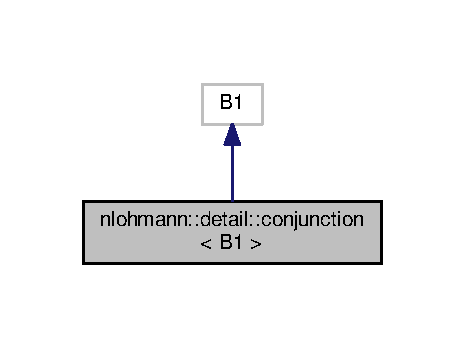
\includegraphics[width=223pt]{structnlohmann_1_1detail_1_1conjunction_3_01_b1_01_4__inherit__graph}
\end{center}
\end{figure}


Collaboration diagram for nlohmann\+:\+:detail\+:\+:conjunction$<$ B1 $>$\+:\nopagebreak
\begin{figure}[H]
\begin{center}
\leavevmode
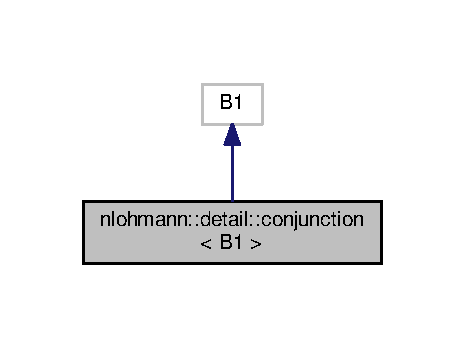
\includegraphics[width=223pt]{structnlohmann_1_1detail_1_1conjunction_3_01_b1_01_4__coll__graph}
\end{center}
\end{figure}


\subsection{Detailed Description}
\subsubsection*{template$<$class B1$>$\\*
struct nlohmann\+::detail\+::conjunction$<$ B1 $>$}



Definition at line 539 of file json.\+hpp.



The documentation for this struct was generated from the following file\+:\begin{DoxyCompactItemize}
\item 
include/\hyperlink{json_8hpp}{json.\+hpp}\end{DoxyCompactItemize}

\hypertarget{structnlohmann_1_1detail_1_1conjunction_3_01_b1_00_01_bn_8_8_8_01_4}{}\section{nlohmann\+:\+:detail\+:\+:conjunction$<$ B1, Bn... $>$ Struct Template Reference}
\label{structnlohmann_1_1detail_1_1conjunction_3_01_b1_00_01_bn_8_8_8_01_4}\index{nlohmann\+::detail\+::conjunction$<$ B1, Bn... $>$@{nlohmann\+::detail\+::conjunction$<$ B1, Bn... $>$}}


{\ttfamily \#include $<$json.\+hpp$>$}



Inheritance diagram for nlohmann\+:\+:detail\+:\+:conjunction$<$ B1, Bn... $>$\+:\nopagebreak
\begin{figure}[H]
\begin{center}
\leavevmode
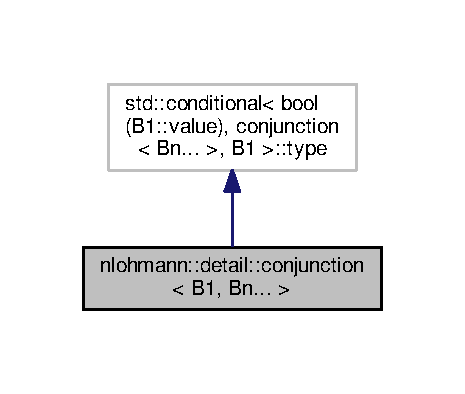
\includegraphics[width=223pt]{structnlohmann_1_1detail_1_1conjunction_3_01_b1_00_01_bn_8_8_8_01_4__inherit__graph}
\end{center}
\end{figure}


Collaboration diagram for nlohmann\+:\+:detail\+:\+:conjunction$<$ B1, Bn... $>$\+:\nopagebreak
\begin{figure}[H]
\begin{center}
\leavevmode
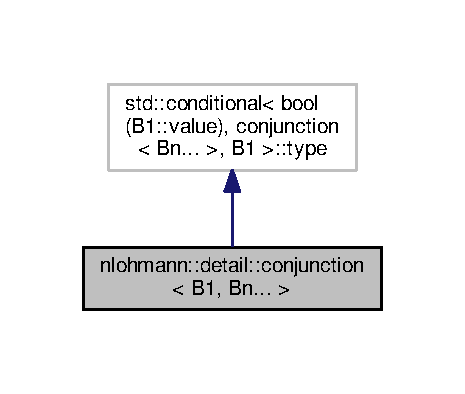
\includegraphics[width=223pt]{structnlohmann_1_1detail_1_1conjunction_3_01_b1_00_01_bn_8_8_8_01_4__coll__graph}
\end{center}
\end{figure}


\subsection{Detailed Description}
\subsubsection*{template$<$class B1, class... Bn$>$\\*
struct nlohmann\+::detail\+::conjunction$<$ B1, Bn... $>$}



Definition at line 541 of file json.\+hpp.



The documentation for this struct was generated from the following file\+:\begin{DoxyCompactItemize}
\item 
include/\hyperlink{json_8hpp}{json.\+hpp}\end{DoxyCompactItemize}

\hypertarget{class_couch_d_b}{}\section{Couch\+DB Class Reference}
\label{class_couch_d_b}\index{Couch\+DB@{Couch\+DB}}


{\ttfamily \#include $<$Couch\+D\+B.\+hpp$>$}



Inheritance diagram for Couch\+DB\+:\nopagebreak
\begin{figure}[H]
\begin{center}
\leavevmode
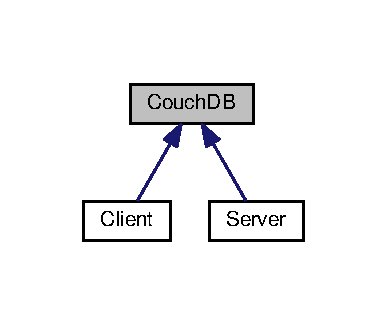
\includegraphics[width=186pt]{class_couch_d_b__inherit__graph}
\end{center}
\end{figure}


Collaboration diagram for Couch\+DB\+:\nopagebreak
\begin{figure}[H]
\begin{center}
\leavevmode
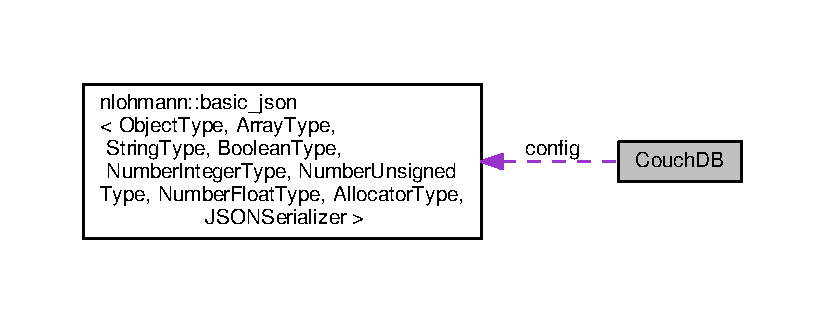
\includegraphics[width=350pt]{class_couch_d_b__coll__graph}
\end{center}
\end{figure}
\subsection*{Protected Member Functions}
\begin{DoxyCompactItemize}
\item 
bool \hyperlink{class_couch_d_b_a71bc84918bdd964da859a844ef00fe11}{H\+T\+T\+P\+G\+ET} (std\+::string url\+\_\+, std\+::string $\ast$ret)
\begin{DoxyCompactList}\small\item\em H\+T\+TP G\+ET function. \end{DoxyCompactList}\item 
bool \hyperlink{class_couch_d_b_a51e32342b653c055a19602a716f2fb7c}{H\+T\+T\+P\+P\+UT} (std\+::string url\+\_\+, std\+::string data)
\begin{DoxyCompactList}\small\item\em H\+T\+TP P\+UT function. \end{DoxyCompactList}\item 
bool \hyperlink{class_couch_d_b_a1aa5d75023ff39b9ebf04b1dbee500f3}{H\+T\+T\+P\+P\+O\+ST} (std\+::string url\+\_\+, std\+::string data)
\begin{DoxyCompactList}\small\item\em H\+T\+TP P\+O\+ST function. \end{DoxyCompactList}\item 
bool \hyperlink{class_couch_d_b_ab4bb23537894cbc90adfc736fad836a0}{H\+T\+T\+P\+D\+E\+L\+E\+TE} (std\+::string url\+\_\+)
\begin{DoxyCompactList}\small\item\em H\+T\+TP D\+E\+L\+E\+TE function. \end{DoxyCompactList}\end{DoxyCompactItemize}
\subsection*{Static Protected Member Functions}
\begin{DoxyCompactItemize}
\item 
static size\+\_\+t \hyperlink{class_couch_d_b_a6216c074f7062f4098e7ab3e848a6c3d}{Callback\+Func} (void $\ast$contents, size\+\_\+t size, size\+\_\+t nmemb, std\+::string $\ast$s)
\begin{DoxyCompactList}\small\item\em Callback function for curl H\+T\+TP calls. Sends output into string. Should not be called outside of C\+U\+R\+L\+O\+P\+T\+\_\+\+W\+R\+I\+T\+E\+F\+U\+N\+C\+T\+I\+ON. \end{DoxyCompactList}\end{DoxyCompactItemize}
\subsection*{Protected Attributes}
\begin{DoxyCompactItemize}
\item 
std\+::string \hyperlink{class_couch_d_b_a1282b49d828b838b8007bbb08ba77a69}{url}
\item 
std\+::string \hyperlink{class_couch_d_b_a5951cb721e50d0b8d24c8fea625909ff}{database}
\item 
\hyperlink{_couch_d_b_8hpp_ab701e3ac61a85b337ec5c1abaad6742d}{json} \hyperlink{class_couch_d_b_ada3dd3c5112ccf493eafe278ce4a521c}{config}
\end{DoxyCompactItemize}


\subsection{Detailed Description}


Definition at line 19 of file Couch\+D\+B.\+hpp.



\subsection{Member Function Documentation}
\index{Couch\+DB@{Couch\+DB}!Callback\+Func@{Callback\+Func}}
\index{Callback\+Func@{Callback\+Func}!Couch\+DB@{Couch\+DB}}
\subsubsection[{\texorpdfstring{Callback\+Func(void $\ast$contents, size\+\_\+t size, size\+\_\+t nmemb, std\+::string $\ast$s)}{CallbackFunc(void *contents, size_t size, size_t nmemb, std::string *s)}}]{\setlength{\rightskip}{0pt plus 5cm}size\+\_\+t Couch\+D\+B\+::\+Callback\+Func (
\begin{DoxyParamCaption}
\item[{void $\ast$}]{contents, }
\item[{size\+\_\+t}]{size, }
\item[{size\+\_\+t}]{nmemb, }
\item[{std\+::string $\ast$}]{s}
\end{DoxyParamCaption}
)\hspace{0.3cm}{\ttfamily [static]}, {\ttfamily [protected]}}\hypertarget{class_couch_d_b_a6216c074f7062f4098e7ab3e848a6c3d}{}\label{class_couch_d_b_a6216c074f7062f4098e7ab3e848a6c3d}


Callback function for curl H\+T\+TP calls. Sends output into string. Should not be called outside of C\+U\+R\+L\+O\+P\+T\+\_\+\+W\+R\+I\+T\+E\+F\+U\+N\+C\+T\+I\+ON. 



Definition at line 13 of file Couch\+D\+B.\+cpp.

\index{Couch\+DB@{Couch\+DB}!H\+T\+T\+P\+D\+E\+L\+E\+TE@{H\+T\+T\+P\+D\+E\+L\+E\+TE}}
\index{H\+T\+T\+P\+D\+E\+L\+E\+TE@{H\+T\+T\+P\+D\+E\+L\+E\+TE}!Couch\+DB@{Couch\+DB}}
\subsubsection[{\texorpdfstring{H\+T\+T\+P\+D\+E\+L\+E\+T\+E(std\+::string url\+\_\+)}{HTTPDELETE(std::string url_)}}]{\setlength{\rightskip}{0pt plus 5cm}bool Couch\+D\+B\+::\+H\+T\+T\+P\+D\+E\+L\+E\+TE (
\begin{DoxyParamCaption}
\item[{std\+::string}]{url\+\_\+}
\end{DoxyParamCaption}
)\hspace{0.3cm}{\ttfamily [protected]}}\hypertarget{class_couch_d_b_ab4bb23537894cbc90adfc736fad836a0}{}\label{class_couch_d_b_ab4bb23537894cbc90adfc736fad836a0}


H\+T\+TP D\+E\+L\+E\+TE function. 


\begin{DoxyParams}{Parameters}
{\em url\+\_\+} & -\/ U\+RL of file to delete. \\
\hline
\end{DoxyParams}


Definition at line 110 of file Couch\+D\+B.\+cpp.

\index{Couch\+DB@{Couch\+DB}!H\+T\+T\+P\+G\+ET@{H\+T\+T\+P\+G\+ET}}
\index{H\+T\+T\+P\+G\+ET@{H\+T\+T\+P\+G\+ET}!Couch\+DB@{Couch\+DB}}
\subsubsection[{\texorpdfstring{H\+T\+T\+P\+G\+E\+T(std\+::string url\+\_\+, std\+::string $\ast$ret)}{HTTPGET(std::string url_, std::string *ret)}}]{\setlength{\rightskip}{0pt plus 5cm}bool Couch\+D\+B\+::\+H\+T\+T\+P\+G\+ET (
\begin{DoxyParamCaption}
\item[{std\+::string}]{url\+\_\+, }
\item[{std\+::string $\ast$}]{ret}
\end{DoxyParamCaption}
)\hspace{0.3cm}{\ttfamily [protected]}}\hypertarget{class_couch_d_b_a71bc84918bdd964da859a844ef00fe11}{}\label{class_couch_d_b_a71bc84918bdd964da859a844ef00fe11}


H\+T\+TP G\+ET function. 


\begin{DoxyParams}{Parameters}
{\em url\+\_\+} & -\/ U\+RL to get from. \\
\hline
\end{DoxyParams}
\begin{DoxyReturn}{Returns}
String of output from call. 
\end{DoxyReturn}


Definition at line 31 of file Couch\+D\+B.\+cpp.

\index{Couch\+DB@{Couch\+DB}!H\+T\+T\+P\+P\+O\+ST@{H\+T\+T\+P\+P\+O\+ST}}
\index{H\+T\+T\+P\+P\+O\+ST@{H\+T\+T\+P\+P\+O\+ST}!Couch\+DB@{Couch\+DB}}
\subsubsection[{\texorpdfstring{H\+T\+T\+P\+P\+O\+S\+T(std\+::string url\+\_\+, std\+::string data)}{HTTPPOST(std::string url_, std::string data)}}]{\setlength{\rightskip}{0pt plus 5cm}bool Couch\+D\+B\+::\+H\+T\+T\+P\+P\+O\+ST (
\begin{DoxyParamCaption}
\item[{std\+::string}]{url\+\_\+, }
\item[{std\+::string}]{data}
\end{DoxyParamCaption}
)\hspace{0.3cm}{\ttfamily [protected]}}\hypertarget{class_couch_d_b_a1aa5d75023ff39b9ebf04b1dbee500f3}{}\label{class_couch_d_b_a1aa5d75023ff39b9ebf04b1dbee500f3}


H\+T\+TP P\+O\+ST function. 


\begin{DoxyParams}{Parameters}
{\em url\+\_\+} & -\/ U\+RL to post data. \\
\hline
{\em data} & -\/ Data to be posted into file. \\
\hline
\end{DoxyParams}


Definition at line 80 of file Couch\+D\+B.\+cpp.

\index{Couch\+DB@{Couch\+DB}!H\+T\+T\+P\+P\+UT@{H\+T\+T\+P\+P\+UT}}
\index{H\+T\+T\+P\+P\+UT@{H\+T\+T\+P\+P\+UT}!Couch\+DB@{Couch\+DB}}
\subsubsection[{\texorpdfstring{H\+T\+T\+P\+P\+U\+T(std\+::string url\+\_\+, std\+::string data)}{HTTPPUT(std::string url_, std::string data)}}]{\setlength{\rightskip}{0pt plus 5cm}bool Couch\+D\+B\+::\+H\+T\+T\+P\+P\+UT (
\begin{DoxyParamCaption}
\item[{std\+::string}]{url\+\_\+, }
\item[{std\+::string}]{data}
\end{DoxyParamCaption}
)\hspace{0.3cm}{\ttfamily [protected]}}\hypertarget{class_couch_d_b_a51e32342b653c055a19602a716f2fb7c}{}\label{class_couch_d_b_a51e32342b653c055a19602a716f2fb7c}


H\+T\+TP P\+UT function. 


\begin{DoxyParams}{Parameters}
{\em url\+\_\+} & -\/ U\+RL to put data. \\
\hline
{\em data} & -\/ Data to be put into file. \\
\hline
\end{DoxyParams}


Definition at line 54 of file Couch\+D\+B.\+cpp.



\subsection{Member Data Documentation}
\index{Couch\+DB@{Couch\+DB}!config@{config}}
\index{config@{config}!Couch\+DB@{Couch\+DB}}
\subsubsection[{\texorpdfstring{config}{config}}]{\setlength{\rightskip}{0pt plus 5cm}{\bf json} Couch\+D\+B\+::config\hspace{0.3cm}{\ttfamily [protected]}}\hypertarget{class_couch_d_b_ada3dd3c5112ccf493eafe278ce4a521c}{}\label{class_couch_d_b_ada3dd3c5112ccf493eafe278ce4a521c}


Definition at line 23 of file Couch\+D\+B.\+hpp.

\index{Couch\+DB@{Couch\+DB}!database@{database}}
\index{database@{database}!Couch\+DB@{Couch\+DB}}
\subsubsection[{\texorpdfstring{database}{database}}]{\setlength{\rightskip}{0pt plus 5cm}std\+::string Couch\+D\+B\+::database\hspace{0.3cm}{\ttfamily [protected]}}\hypertarget{class_couch_d_b_a5951cb721e50d0b8d24c8fea625909ff}{}\label{class_couch_d_b_a5951cb721e50d0b8d24c8fea625909ff}


Definition at line 22 of file Couch\+D\+B.\+hpp.

\index{Couch\+DB@{Couch\+DB}!url@{url}}
\index{url@{url}!Couch\+DB@{Couch\+DB}}
\subsubsection[{\texorpdfstring{url}{url}}]{\setlength{\rightskip}{0pt plus 5cm}std\+::string Couch\+D\+B\+::url\hspace{0.3cm}{\ttfamily [protected]}}\hypertarget{class_couch_d_b_a1282b49d828b838b8007bbb08ba77a69}{}\label{class_couch_d_b_a1282b49d828b838b8007bbb08ba77a69}


Definition at line 21 of file Couch\+D\+B.\+hpp.



The documentation for this class was generated from the following files\+:\begin{DoxyCompactItemize}
\item 
include/\hyperlink{_couch_d_b_8hpp}{Couch\+D\+B.\+hpp}\item 
src/\hyperlink{_couch_d_b_8cpp}{Couch\+D\+B.\+cpp}\end{DoxyCompactItemize}

\hypertarget{class_diagnostics}{}\section{Diagnostics Class Reference}
\label{class_diagnostics}\index{Diagnostics@{Diagnostics}}


{\ttfamily \#include $<$diagnostics.\+hpp$>$}

\subsection*{Public Member Functions}
\begin{DoxyCompactItemize}
\item 
\hyperlink{class_diagnostics_a84423ad40c376ce8d8a4f02dc0b7f44c}{Diagnostics} (void)
\begin{DoxyCompactList}\small\item\em Constructor function if library has yet to initialised. \end{DoxyCompactList}\item 
\hyperlink{class_diagnostics_ab4cf66446bf7d4af44315629de9a910b}{Diagnostics} (uint32\+\_\+t h)
\begin{DoxyCompactList}\small\item\em Constructor function if library has already been initialised but diagnostics need to be performed. \end{DoxyCompactList}\item 
\hyperlink{class_diagnostics_ad05cd98138d8ef3a0c1284412fbddd6b}{$\sim$\+Diagnostics} ()
\begin{DoxyCompactList}\small\item\em Class destructor. \end{DoxyCompactList}\item 
void \hyperlink{class_diagnostics_a8263e91e26d536a03442d59e6c5b0d12}{print\+Board\+Info} (void)
\item 
void \hyperlink{class_diagnostics_a686255ad134138a830d0b917334cb264}{print\+Board\+Temperatures} (void)
\item 
void \hyperlink{class_diagnostics_af25cdb55c895228c3d312345e1782c55}{print\+I2\+C\+Support} (void)
\end{DoxyCompactItemize}


\subsection{Detailed Description}
S\+E\+MA diagnostics class. Displays useful information about the board. 

Definition at line 18 of file diagnostics.\+hpp.



\subsection{Constructor \& Destructor Documentation}
\index{Diagnostics@{Diagnostics}!Diagnostics@{Diagnostics}}
\index{Diagnostics@{Diagnostics}!Diagnostics@{Diagnostics}}
\subsubsection[{\texorpdfstring{Diagnostics(void)}{Diagnostics(void)}}]{\setlength{\rightskip}{0pt plus 5cm}Diagnostics\+::\+Diagnostics (
\begin{DoxyParamCaption}
\item[{void}]{}
\end{DoxyParamCaption}
)}\hypertarget{class_diagnostics_a84423ad40c376ce8d8a4f02dc0b7f44c}{}\label{class_diagnostics_a84423ad40c376ce8d8a4f02dc0b7f44c}


Constructor function if library has yet to initialised. 



Definition at line 13 of file diagnostics.\+cpp.

\index{Diagnostics@{Diagnostics}!Diagnostics@{Diagnostics}}
\index{Diagnostics@{Diagnostics}!Diagnostics@{Diagnostics}}
\subsubsection[{\texorpdfstring{Diagnostics(uint32\+\_\+t h)}{Diagnostics(uint32_t h)}}]{\setlength{\rightskip}{0pt plus 5cm}Diagnostics\+::\+Diagnostics (
\begin{DoxyParamCaption}
\item[{uint32\+\_\+t}]{h}
\end{DoxyParamCaption}
)}\hypertarget{class_diagnostics_ab4cf66446bf7d4af44315629de9a910b}{}\label{class_diagnostics_ab4cf66446bf7d4af44315629de9a910b}


Constructor function if library has already been initialised but diagnostics need to be performed. 



Definition at line 27 of file diagnostics.\+cpp.

\index{Diagnostics@{Diagnostics}!````~Diagnostics@{$\sim$\+Diagnostics}}
\index{````~Diagnostics@{$\sim$\+Diagnostics}!Diagnostics@{Diagnostics}}
\subsubsection[{\texorpdfstring{$\sim$\+Diagnostics()}{~Diagnostics()}}]{\setlength{\rightskip}{0pt plus 5cm}Diagnostics\+::$\sim$\+Diagnostics (
\begin{DoxyParamCaption}
\item[{void}]{}
\end{DoxyParamCaption}
)}\hypertarget{class_diagnostics_ad05cd98138d8ef3a0c1284412fbddd6b}{}\label{class_diagnostics_ad05cd98138d8ef3a0c1284412fbddd6b}


Class destructor. 



Definition at line 35 of file diagnostics.\+cpp.



\subsection{Member Function Documentation}
\index{Diagnostics@{Diagnostics}!print\+Board\+Info@{print\+Board\+Info}}
\index{print\+Board\+Info@{print\+Board\+Info}!Diagnostics@{Diagnostics}}
\subsubsection[{\texorpdfstring{print\+Board\+Info(void)}{printBoardInfo(void)}}]{\setlength{\rightskip}{0pt plus 5cm}void Diagnostics\+::print\+Board\+Info (
\begin{DoxyParamCaption}
\item[{void}]{}
\end{DoxyParamCaption}
)}\hypertarget{class_diagnostics_a8263e91e26d536a03442d59e6c5b0d12}{}\label{class_diagnostics_a8263e91e26d536a03442d59e6c5b0d12}
Print selcted information about the C\+O\+M-\/e board. Current information printed\+: \hyperlink{class_board}{Board} Manufacturer and \hyperlink{class_board}{Board} Name. 

Definition at line 45 of file diagnostics.\+cpp.

\index{Diagnostics@{Diagnostics}!print\+Board\+Temperatures@{print\+Board\+Temperatures}}
\index{print\+Board\+Temperatures@{print\+Board\+Temperatures}!Diagnostics@{Diagnostics}}
\subsubsection[{\texorpdfstring{print\+Board\+Temperatures(void)}{printBoardTemperatures(void)}}]{\setlength{\rightskip}{0pt plus 5cm}void Diagnostics\+::print\+Board\+Temperatures (
\begin{DoxyParamCaption}
\item[{void}]{}
\end{DoxyParamCaption}
)}\hypertarget{class_diagnostics_a686255ad134138a830d0b917334cb264}{}\label{class_diagnostics_a686255ad134138a830d0b917334cb264}
Print current board and C\+PU temperatures. 

Definition at line 54 of file diagnostics.\+cpp.

\index{Diagnostics@{Diagnostics}!print\+I2\+C\+Support@{print\+I2\+C\+Support}}
\index{print\+I2\+C\+Support@{print\+I2\+C\+Support}!Diagnostics@{Diagnostics}}
\subsubsection[{\texorpdfstring{print\+I2\+C\+Support(void)}{printI2CSupport(void)}}]{\setlength{\rightskip}{0pt plus 5cm}void Diagnostics\+::print\+I2\+C\+Support (
\begin{DoxyParamCaption}
\item[{void}]{}
\end{DoxyParamCaption}
)}\hypertarget{class_diagnostics_af25cdb55c895228c3d312345e1782c55}{}\label{class_diagnostics_af25cdb55c895228c3d312345e1782c55}
Print available I2C buses. 

Definition at line 63 of file diagnostics.\+cpp.



The documentation for this class was generated from the following files\+:\begin{DoxyCompactItemize}
\item 
include/\hyperlink{diagnostics_8hpp}{diagnostics.\+hpp}\item 
src/\hyperlink{diagnostics_8cpp}{diagnostics.\+cpp}\end{DoxyCompactItemize}

\hypertarget{class_d_s3232_temperature_i2_c_register}{}\section{D\+S3232\+Temperature\+I2\+C\+Register Class Reference}
\label{class_d_s3232_temperature_i2_c_register}\index{D\+S3232\+Temperature\+I2\+C\+Register@{D\+S3232\+Temperature\+I2\+C\+Register}}


{\ttfamily \#include $<$I2\+C\+Register.\+hpp$>$}



Inheritance diagram for D\+S3232\+Temperature\+I2\+C\+Register\+:\nopagebreak
\begin{figure}[H]
\begin{center}
\leavevmode
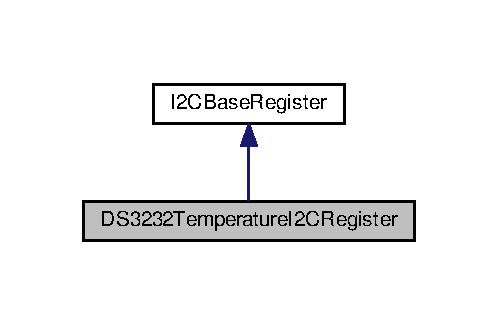
\includegraphics[width=239pt]{class_d_s3232_temperature_i2_c_register__inherit__graph}
\end{center}
\end{figure}


Collaboration diagram for D\+S3232\+Temperature\+I2\+C\+Register\+:\nopagebreak
\begin{figure}[H]
\begin{center}
\leavevmode
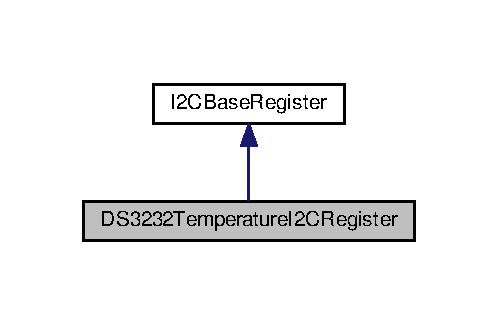
\includegraphics[width=239pt]{class_d_s3232_temperature_i2_c_register__coll__graph}
\end{center}
\end{figure}
\subsection*{Public Member Functions}
\begin{DoxyCompactItemize}
\item 
\hyperlink{class_d_s3232_temperature_i2_c_register_a45e6afc23e8218b5b340d89c901441c4}{D\+S3232\+Temperature\+I2\+C\+Register} (uint32\+\_\+t addr, std\+::string rw, std\+::function$<$ \hyperlink{units__define_8hpp_a95d46867fa79633565c288a0b4bd5408}{units\+\_\+variant}(double)$>$ read\+\_\+func, std\+::function$<$ uint8\+\_\+t(\hyperlink{units__define_8hpp_a95d46867fa79633565c288a0b4bd5408}{units\+\_\+variant})$>$ write\+\_\+func)
\begin{DoxyCompactList}\small\item\em Class constructor. \end{DoxyCompactList}\item 
\hyperlink{class_d_s3232_temperature_i2_c_register_a58d1a1797e2d18138a7ee53c4b89036d}{$\sim$\+D\+S3232\+Temperature\+I2\+C\+Register} (void)
\begin{DoxyCompactList}\small\item\em Class destructor. \end{DoxyCompactList}\item 
\hyperlink{units__define_8hpp_a95d46867fa79633565c288a0b4bd5408}{units\+\_\+variant} \hyperlink{class_d_s3232_temperature_i2_c_register_ab8733916ac8d733eb8d0e2b72df4efc2}{read} (\hyperlink{class_i2_c__base}{I2\+C\+\_\+base} $\ast$i2c\+\_\+ptr, uint32\+\_\+t address)
\begin{DoxyCompactList}\small\item\em Read data from register. \end{DoxyCompactList}\item 
void \hyperlink{class_d_s3232_temperature_i2_c_register_a69c3e1c321d2161d8c69e984031d7fc8}{write} (\hyperlink{class_i2_c__base}{I2\+C\+\_\+base} $\ast$i2c\+\_\+ptr, uint32\+\_\+t address, \hyperlink{units__define_8hpp_a95d46867fa79633565c288a0b4bd5408}{units\+\_\+variant} value)
\begin{DoxyCompactList}\small\item\em Write data to register. \end{DoxyCompactList}\end{DoxyCompactItemize}
\subsection*{Additional Inherited Members}


\subsection{Detailed Description}
Derived \hyperlink{class_i2_c_base_register}{I2\+C\+Base\+Register} class for calls to D\+S3232 temperature register. 

Definition at line 62 of file I2\+C\+Register.\+hpp.



\subsection{Constructor \& Destructor Documentation}
\index{D\+S3232\+Temperature\+I2\+C\+Register@{D\+S3232\+Temperature\+I2\+C\+Register}!D\+S3232\+Temperature\+I2\+C\+Register@{D\+S3232\+Temperature\+I2\+C\+Register}}
\index{D\+S3232\+Temperature\+I2\+C\+Register@{D\+S3232\+Temperature\+I2\+C\+Register}!D\+S3232\+Temperature\+I2\+C\+Register@{D\+S3232\+Temperature\+I2\+C\+Register}}
\subsubsection[{\texorpdfstring{D\+S3232\+Temperature\+I2\+C\+Register(uint32\+\_\+t addr, std\+::string rw, std\+::function$<$ units\+\_\+variant(double)$>$ read\+\_\+func, std\+::function$<$ uint8\+\_\+t(units\+\_\+variant)$>$ write\+\_\+func)}{DS3232TemperatureI2CRegister(uint32_t addr, std::string rw, std::function< units_variant(double)> read_func, std::function< uint8_t(units_variant)> write_func)}}]{\setlength{\rightskip}{0pt plus 5cm}D\+S3232\+Temperature\+I2\+C\+Register\+::\+D\+S3232\+Temperature\+I2\+C\+Register (
\begin{DoxyParamCaption}
\item[{uint32\+\_\+t}]{r, }
\item[{std\+::string}]{rw, }
\item[{std\+::function$<$ {\bf units\+\_\+variant}(double)$>$}]{read\+\_\+func, }
\item[{std\+::function$<$ uint8\+\_\+t({\bf units\+\_\+variant})$>$}]{write\+\_\+func}
\end{DoxyParamCaption}
)}\hypertarget{class_d_s3232_temperature_i2_c_register_a45e6afc23e8218b5b340d89c901441c4}{}\label{class_d_s3232_temperature_i2_c_register_a45e6afc23e8218b5b340d89c901441c4}


Class constructor. 


\begin{DoxyParams}{Parameters}
{\em r} & -\/ Address of register within I2C device. \\
\hline
{\em read\+\_\+func} & -\/ Lambda function to convert hexadecimal value into correct units type. \\
\hline
{\em write\+\_\+func} & -\/ Lambda function to convert units type into uint8\+\_\+t to be written. \\
\hline
\end{DoxyParams}


Definition at line 72 of file D\+S3232\+Registers.\+cpp.

\index{D\+S3232\+Temperature\+I2\+C\+Register@{D\+S3232\+Temperature\+I2\+C\+Register}!````~D\+S3232\+Temperature\+I2\+C\+Register@{$\sim$\+D\+S3232\+Temperature\+I2\+C\+Register}}
\index{````~D\+S3232\+Temperature\+I2\+C\+Register@{$\sim$\+D\+S3232\+Temperature\+I2\+C\+Register}!D\+S3232\+Temperature\+I2\+C\+Register@{D\+S3232\+Temperature\+I2\+C\+Register}}
\subsubsection[{\texorpdfstring{$\sim$\+D\+S3232\+Temperature\+I2\+C\+Register(void)}{~DS3232TemperatureI2CRegister(void)}}]{\setlength{\rightskip}{0pt plus 5cm}D\+S3232\+Temperature\+I2\+C\+Register\+::$\sim$\+D\+S3232\+Temperature\+I2\+C\+Register (
\begin{DoxyParamCaption}
\item[{void}]{}
\end{DoxyParamCaption}
)}\hypertarget{class_d_s3232_temperature_i2_c_register_a58d1a1797e2d18138a7ee53c4b89036d}{}\label{class_d_s3232_temperature_i2_c_register_a58d1a1797e2d18138a7ee53c4b89036d}


Class destructor. 



Definition at line 88 of file D\+S3232\+Registers.\+cpp.



\subsection{Member Function Documentation}
\index{D\+S3232\+Temperature\+I2\+C\+Register@{D\+S3232\+Temperature\+I2\+C\+Register}!read@{read}}
\index{read@{read}!D\+S3232\+Temperature\+I2\+C\+Register@{D\+S3232\+Temperature\+I2\+C\+Register}}
\subsubsection[{\texorpdfstring{read(\+I2\+C\+\_\+base $\ast$i2c\+\_\+ptr, uint32\+\_\+t address)}{read(I2C_base *i2c_ptr, uint32_t address)}}]{\setlength{\rightskip}{0pt plus 5cm}{\bf units\+\_\+variant} D\+S3232\+Temperature\+I2\+C\+Register\+::read (
\begin{DoxyParamCaption}
\item[{{\bf I2\+C\+\_\+base} $\ast$}]{i2c\+\_\+ptr, }
\item[{uint32\+\_\+t}]{address}
\end{DoxyParamCaption}
)\hspace{0.3cm}{\ttfamily [virtual]}}\hypertarget{class_d_s3232_temperature_i2_c_register_ab8733916ac8d733eb8d0e2b72df4efc2}{}\label{class_d_s3232_temperature_i2_c_register_ab8733916ac8d733eb8d0e2b72df4efc2}


Read data from register. 


\begin{DoxyParams}{Parameters}
{\em i2c\+\_\+ptr} & -\/ Pointer to \hyperlink{class_i2_c__base}{I2\+C\+\_\+base} class used for transport. \\
\hline
\end{DoxyParams}
\begin{DoxyReturn}{Returns}
units\+\_\+variant containing quantity of correct type. 
\end{DoxyReturn}


Implements \hyperlink{class_i2_c_base_register_a947d834a745d3036c4cd8a2d5e19cd0d}{I2\+C\+Base\+Register}.



Definition at line 95 of file D\+S3232\+Registers.\+cpp.

\index{D\+S3232\+Temperature\+I2\+C\+Register@{D\+S3232\+Temperature\+I2\+C\+Register}!write@{write}}
\index{write@{write}!D\+S3232\+Temperature\+I2\+C\+Register@{D\+S3232\+Temperature\+I2\+C\+Register}}
\subsubsection[{\texorpdfstring{write(\+I2\+C\+\_\+base $\ast$i2c\+\_\+ptr, uint32\+\_\+t address, units\+\_\+variant value)}{write(I2C_base *i2c_ptr, uint32_t address, units_variant value)}}]{\setlength{\rightskip}{0pt plus 5cm}void D\+S3232\+Temperature\+I2\+C\+Register\+::write (
\begin{DoxyParamCaption}
\item[{{\bf I2\+C\+\_\+base} $\ast$}]{i2c\+\_\+ptr, }
\item[{uint32\+\_\+t}]{address, }
\item[{{\bf units\+\_\+variant}}]{value}
\end{DoxyParamCaption}
)\hspace{0.3cm}{\ttfamily [virtual]}}\hypertarget{class_d_s3232_temperature_i2_c_register_a69c3e1c321d2161d8c69e984031d7fc8}{}\label{class_d_s3232_temperature_i2_c_register_a69c3e1c321d2161d8c69e984031d7fc8}


Write data to register. 


\begin{DoxyParams}{Parameters}
{\em i2c\+\_\+ptr} & -\/ Pointer to \hyperlink{class_i2_c__base}{I2\+C\+\_\+base} class used for transport. \\
\hline
{\em value} & -\/ Data to be written. Must be of correct type. \\
\hline
\end{DoxyParams}


Implements \hyperlink{class_i2_c_base_register_ad3f9f1404fe6af3e10e8f204b16d2066}{I2\+C\+Base\+Register}.



Definition at line 115 of file D\+S3232\+Registers.\+cpp.



The documentation for this class was generated from the following files\+:\begin{DoxyCompactItemize}
\item 
include/\hyperlink{_i2_c_register_8hpp}{I2\+C\+Register.\+hpp}\item 
src/\hyperlink{_d_s3232_registers_8cpp}{D\+S3232\+Registers.\+cpp}\end{DoxyCompactItemize}

\hypertarget{classnlohmann_1_1detail_1_1exception}{}\section{nlohmann\+:\+:detail\+:\+:exception Class Reference}
\label{classnlohmann_1_1detail_1_1exception}\index{nlohmann\+::detail\+::exception@{nlohmann\+::detail\+::exception}}


general exception of the \hyperlink{classnlohmann_1_1basic__json}{basic\+\_\+json} class  




{\ttfamily \#include $<$json.\+hpp$>$}



Inheritance diagram for nlohmann\+:\+:detail\+:\+:exception\+:\nopagebreak
\begin{figure}[H]
\begin{center}
\leavevmode
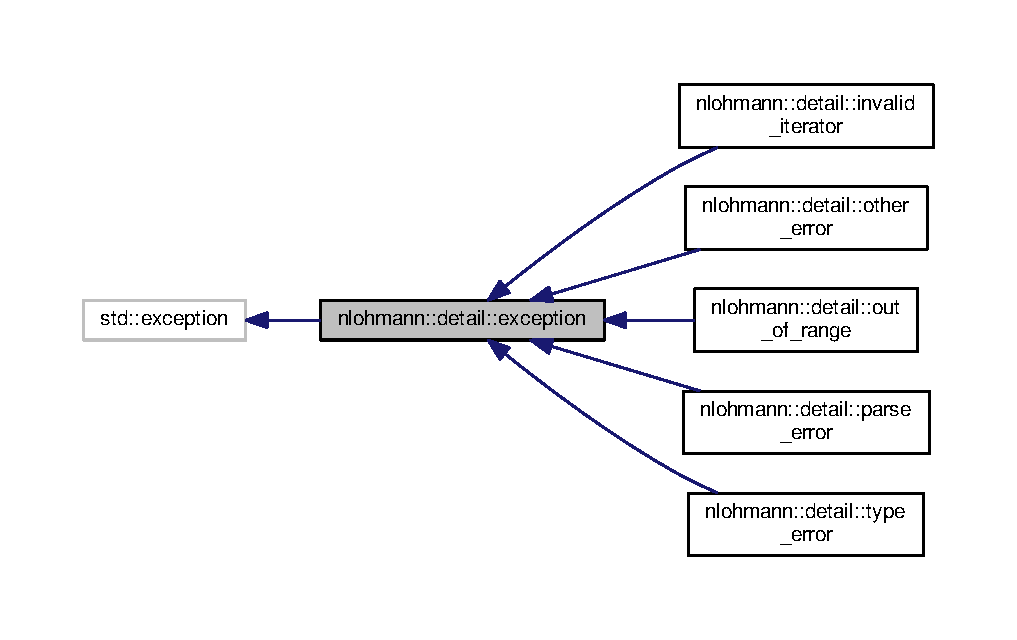
\includegraphics[width=350pt]{classnlohmann_1_1detail_1_1exception__inherit__graph}
\end{center}
\end{figure}


Collaboration diagram for nlohmann\+:\+:detail\+:\+:exception\+:\nopagebreak
\begin{figure}[H]
\begin{center}
\leavevmode
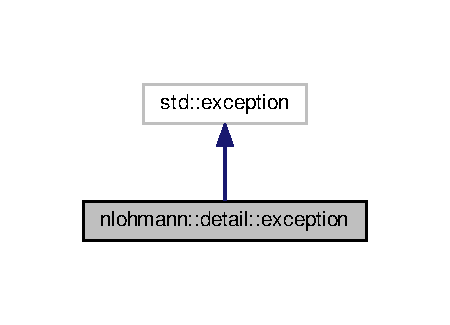
\includegraphics[width=216pt]{classnlohmann_1_1detail_1_1exception__coll__graph}
\end{center}
\end{figure}
\subsection*{Public Member Functions}
\begin{DoxyCompactItemize}
\item 
const char $\ast$ \hyperlink{classnlohmann_1_1detail_1_1exception_a56e006c6ac214875115049ae5b9b569a}{what} () const noexceptoverride
\begin{DoxyCompactList}\small\item\em returns the explanatory string \end{DoxyCompactList}\end{DoxyCompactItemize}
\subsection*{Public Attributes}
\begin{DoxyCompactItemize}
\item 
const int \hyperlink{classnlohmann_1_1detail_1_1exception_a0d4589a3fb54e81646d986c05efa3b9a}{id}
\begin{DoxyCompactList}\small\item\em the id of the exception \end{DoxyCompactList}\end{DoxyCompactItemize}
\subsection*{Protected Member Functions}
\begin{DoxyCompactItemize}
\item 
\hyperlink{classnlohmann_1_1detail_1_1exception_ae323ad0d53bc724414c2233164e65657}{exception} (int id\+\_\+, const char $\ast$what\+\_\+arg)
\end{DoxyCompactItemize}
\subsection*{Static Protected Member Functions}
\begin{DoxyCompactItemize}
\item 
static \hyperlink{namespacenlohmann_1_1detail_a90aa5ef615aa8305e9ea20d8a947980fab45cffe084dd3d20d928bee85e7b0f21}{std\+::string} \hyperlink{classnlohmann_1_1detail_1_1exception_aac7455bbbaed7c01ecd5a2ead336b1ae}{name} (const \hyperlink{namespacenlohmann_1_1detail_a90aa5ef615aa8305e9ea20d8a947980fab45cffe084dd3d20d928bee85e7b0f21}{std\+::string} \&ename, int \hyperlink{classnlohmann_1_1detail_1_1exception_a0d4589a3fb54e81646d986c05efa3b9a}{id})
\end{DoxyCompactItemize}


\subsection{Detailed Description}
general exception of the \hyperlink{classnlohmann_1_1basic__json}{basic\+\_\+json} class 

Extension of std\+::exception objects with a member {\itshape id} for exception ids.

\begin{DoxyNote}{Note}
To have nothrow-\/copy-\/constructible exceptions, we internally use std\+::runtime\+\_\+error which can cope with arbitrary-\/length error messages. Intermediate strings are built with static functions and then passed to the actual constructor.
\end{DoxyNote}
\begin{DoxySince}{Since}
version 3.\+0.\+0 
\end{DoxySince}


Definition at line 177 of file json.\+hpp.



\subsection{Constructor \& Destructor Documentation}
\index{nlohmann\+::detail\+::exception@{nlohmann\+::detail\+::exception}!exception@{exception}}
\index{exception@{exception}!nlohmann\+::detail\+::exception@{nlohmann\+::detail\+::exception}}
\subsubsection[{\texorpdfstring{exception(int id\+\_\+, const char $\ast$what\+\_\+arg)}{exception(int id_, const char *what_arg)}}]{\setlength{\rightskip}{0pt plus 5cm}nlohmann\+::detail\+::exception\+::exception (
\begin{DoxyParamCaption}
\item[{int}]{id\+\_\+, }
\item[{const char $\ast$}]{what\+\_\+arg}
\end{DoxyParamCaption}
)\hspace{0.3cm}{\ttfamily [inline]}, {\ttfamily [protected]}}\hypertarget{classnlohmann_1_1detail_1_1exception_ae323ad0d53bc724414c2233164e65657}{}\label{classnlohmann_1_1detail_1_1exception_ae323ad0d53bc724414c2233164e65657}


Definition at line 190 of file json.\+hpp.



\subsection{Member Function Documentation}
\index{nlohmann\+::detail\+::exception@{nlohmann\+::detail\+::exception}!name@{name}}
\index{name@{name}!nlohmann\+::detail\+::exception@{nlohmann\+::detail\+::exception}}
\subsubsection[{\texorpdfstring{name(const std\+::string \&ename, int id)}{name(const std::string &ename, int id)}}]{\setlength{\rightskip}{0pt plus 5cm}static {\bf std\+::string} nlohmann\+::detail\+::exception\+::name (
\begin{DoxyParamCaption}
\item[{const {\bf std\+::string} \&}]{ename, }
\item[{int}]{id}
\end{DoxyParamCaption}
)\hspace{0.3cm}{\ttfamily [inline]}, {\ttfamily [static]}, {\ttfamily [protected]}}\hypertarget{classnlohmann_1_1detail_1_1exception_aac7455bbbaed7c01ecd5a2ead336b1ae}{}\label{classnlohmann_1_1detail_1_1exception_aac7455bbbaed7c01ecd5a2ead336b1ae}


Definition at line 192 of file json.\+hpp.

\index{nlohmann\+::detail\+::exception@{nlohmann\+::detail\+::exception}!what@{what}}
\index{what@{what}!nlohmann\+::detail\+::exception@{nlohmann\+::detail\+::exception}}
\subsubsection[{\texorpdfstring{what() const noexceptoverride}{what() const noexceptoverride}}]{\setlength{\rightskip}{0pt plus 5cm}const char$\ast$ nlohmann\+::detail\+::exception\+::what (
\begin{DoxyParamCaption}
{}
\end{DoxyParamCaption}
) const\hspace{0.3cm}{\ttfamily [inline]}, {\ttfamily [override]}, {\ttfamily [noexcept]}}\hypertarget{classnlohmann_1_1detail_1_1exception_a56e006c6ac214875115049ae5b9b569a}{}\label{classnlohmann_1_1detail_1_1exception_a56e006c6ac214875115049ae5b9b569a}


returns the explanatory string 



Definition at line 181 of file json.\+hpp.



\subsection{Member Data Documentation}
\index{nlohmann\+::detail\+::exception@{nlohmann\+::detail\+::exception}!id@{id}}
\index{id@{id}!nlohmann\+::detail\+::exception@{nlohmann\+::detail\+::exception}}
\subsubsection[{\texorpdfstring{id}{id}}]{\setlength{\rightskip}{0pt plus 5cm}const int nlohmann\+::detail\+::exception\+::id}\hypertarget{classnlohmann_1_1detail_1_1exception_a0d4589a3fb54e81646d986c05efa3b9a}{}\label{classnlohmann_1_1detail_1_1exception_a0d4589a3fb54e81646d986c05efa3b9a}


the id of the exception 



Definition at line 187 of file json.\+hpp.



The documentation for this class was generated from the following file\+:\begin{DoxyCompactItemize}
\item 
include/\hyperlink{json_8hpp}{json.\+hpp}\end{DoxyCompactItemize}

\hypertarget{structnlohmann_1_1detail_1_1external__constructor}{}\section{nlohmann\+:\+:detail\+:\+:external\+\_\+constructor$<$ value\+\_\+t $>$ Struct Template Reference}
\label{structnlohmann_1_1detail_1_1external__constructor}\index{nlohmann\+::detail\+::external\+\_\+constructor$<$ value\+\_\+t $>$@{nlohmann\+::detail\+::external\+\_\+constructor$<$ value\+\_\+t $>$}}


{\ttfamily \#include $<$json.\+hpp$>$}



\subsection{Detailed Description}
\subsubsection*{template$<$value\+\_\+t$>$\\*
struct nlohmann\+::detail\+::external\+\_\+constructor$<$ value\+\_\+t $>$}



Definition at line 554 of file json.\+hpp.



The documentation for this struct was generated from the following file\+:\begin{DoxyCompactItemize}
\item 
include/\hyperlink{json_8hpp}{json.\+hpp}\end{DoxyCompactItemize}

\hypertarget{structnlohmann_1_1detail_1_1external__constructor_3_01value__t_1_1array_01_4}{}\section{nlohmann\+:\+:detail\+:\+:external\+\_\+constructor$<$ value\+\_\+t\+:\+:array $>$ Struct Template Reference}
\label{structnlohmann_1_1detail_1_1external__constructor_3_01value__t_1_1array_01_4}\index{nlohmann\+::detail\+::external\+\_\+constructor$<$ value\+\_\+t\+::array $>$@{nlohmann\+::detail\+::external\+\_\+constructor$<$ value\+\_\+t\+::array $>$}}


{\ttfamily \#include $<$json.\+hpp$>$}

\subsection*{Static Public Member Functions}
\begin{DoxyCompactItemize}
\item 
{\footnotesize template$<$typename Basic\+Json\+Type $>$ }\\static void \hyperlink{structnlohmann_1_1detail_1_1external__constructor_3_01value__t_1_1array_01_4_abfb2a6eec0bc21e8a7438546aebc55d8}{construct} (Basic\+Json\+Type \&j, const typename Basic\+Json\+Type\+::array\+\_\+t \&arr)
\item 
{\footnotesize template$<$typename Basic\+Json\+Type $>$ }\\static void \hyperlink{structnlohmann_1_1detail_1_1external__constructor_3_01value__t_1_1array_01_4_a50474d6624957a630a1d398cac1e7bfa}{construct} (Basic\+Json\+Type \&j, typename Basic\+Json\+Type\+::array\+\_\+t \&\&arr)
\item 
{\footnotesize template$<$typename Basic\+Json\+Type , typename Compatible\+Array\+Type , enable\+\_\+if\+\_\+t$<$ not std\+::is\+\_\+same$<$ Compatible\+Array\+Type, typename Basic\+Json\+Type\+::array\+\_\+t $>$\+::value, int $>$  = 0$>$ }\\static void \hyperlink{structnlohmann_1_1detail_1_1external__constructor_3_01value__t_1_1array_01_4_a110f50fd5378da876d9a6d6a8d945e37}{construct} (Basic\+Json\+Type \&j, const Compatible\+Array\+Type \&arr)
\item 
{\footnotesize template$<$typename Basic\+Json\+Type $>$ }\\static void \hyperlink{structnlohmann_1_1detail_1_1external__constructor_3_01value__t_1_1array_01_4_a4ebb19b1cb84b4cb224a4c5322e16f14}{construct} (Basic\+Json\+Type \&j, const std\+::vector$<$ bool $>$ \&arr)
\end{DoxyCompactItemize}


\subsection{Detailed Description}
\subsubsection*{template$<$$>$\\*
struct nlohmann\+::detail\+::external\+\_\+constructor$<$ value\+\_\+t\+::array $>$}



Definition at line 625 of file json.\+hpp.



\subsection{Member Function Documentation}
\index{nlohmann\+::detail\+::external\+\_\+constructor$<$ value\+\_\+t\+::array $>$@{nlohmann\+::detail\+::external\+\_\+constructor$<$ value\+\_\+t\+::array $>$}!construct@{construct}}
\index{construct@{construct}!nlohmann\+::detail\+::external\+\_\+constructor$<$ value\+\_\+t\+::array $>$@{nlohmann\+::detail\+::external\+\_\+constructor$<$ value\+\_\+t\+::array $>$}}
\subsubsection[{\texorpdfstring{construct(\+Basic\+Json\+Type \&j, const typename Basic\+Json\+Type\+::array\+\_\+t \&arr)}{construct(BasicJsonType &j, const typename BasicJsonType::array_t &arr)}}]{\setlength{\rightskip}{0pt plus 5cm}template$<$typename Basic\+Json\+Type $>$ static void {\bf nlohmann\+::detail\+::external\+\_\+constructor}$<$ {\bf value\+\_\+t\+::array} $>$\+::construct (
\begin{DoxyParamCaption}
\item[{Basic\+Json\+Type \&}]{j, }
\item[{const typename Basic\+Json\+Type\+::array\+\_\+t \&}]{arr}
\end{DoxyParamCaption}
)\hspace{0.3cm}{\ttfamily [inline]}, {\ttfamily [static]}}\hypertarget{structnlohmann_1_1detail_1_1external__constructor_3_01value__t_1_1array_01_4_abfb2a6eec0bc21e8a7438546aebc55d8}{}\label{structnlohmann_1_1detail_1_1external__constructor_3_01value__t_1_1array_01_4_abfb2a6eec0bc21e8a7438546aebc55d8}


Definition at line 628 of file json.\+hpp.

\index{nlohmann\+::detail\+::external\+\_\+constructor$<$ value\+\_\+t\+::array $>$@{nlohmann\+::detail\+::external\+\_\+constructor$<$ value\+\_\+t\+::array $>$}!construct@{construct}}
\index{construct@{construct}!nlohmann\+::detail\+::external\+\_\+constructor$<$ value\+\_\+t\+::array $>$@{nlohmann\+::detail\+::external\+\_\+constructor$<$ value\+\_\+t\+::array $>$}}
\subsubsection[{\texorpdfstring{construct(\+Basic\+Json\+Type \&j, typename Basic\+Json\+Type\+::array\+\_\+t \&\&arr)}{construct(BasicJsonType &j, typename BasicJsonType::array_t &&arr)}}]{\setlength{\rightskip}{0pt plus 5cm}template$<$typename Basic\+Json\+Type $>$ static void {\bf nlohmann\+::detail\+::external\+\_\+constructor}$<$ {\bf value\+\_\+t\+::array} $>$\+::construct (
\begin{DoxyParamCaption}
\item[{Basic\+Json\+Type \&}]{j, }
\item[{typename Basic\+Json\+Type\+::array\+\_\+t \&\&}]{arr}
\end{DoxyParamCaption}
)\hspace{0.3cm}{\ttfamily [inline]}, {\ttfamily [static]}}\hypertarget{structnlohmann_1_1detail_1_1external__constructor_3_01value__t_1_1array_01_4_a50474d6624957a630a1d398cac1e7bfa}{}\label{structnlohmann_1_1detail_1_1external__constructor_3_01value__t_1_1array_01_4_a50474d6624957a630a1d398cac1e7bfa}


Definition at line 636 of file json.\+hpp.

\index{nlohmann\+::detail\+::external\+\_\+constructor$<$ value\+\_\+t\+::array $>$@{nlohmann\+::detail\+::external\+\_\+constructor$<$ value\+\_\+t\+::array $>$}!construct@{construct}}
\index{construct@{construct}!nlohmann\+::detail\+::external\+\_\+constructor$<$ value\+\_\+t\+::array $>$@{nlohmann\+::detail\+::external\+\_\+constructor$<$ value\+\_\+t\+::array $>$}}
\subsubsection[{\texorpdfstring{construct(\+Basic\+Json\+Type \&j, const Compatible\+Array\+Type \&arr)}{construct(BasicJsonType &j, const CompatibleArrayType &arr)}}]{\setlength{\rightskip}{0pt plus 5cm}template$<$typename Basic\+Json\+Type , typename Compatible\+Array\+Type , enable\+\_\+if\+\_\+t$<$ not std\+::is\+\_\+same$<$ Compatible\+Array\+Type, typename Basic\+Json\+Type\+::array\+\_\+t $>$\+::value, int $>$  = 0$>$ static void {\bf nlohmann\+::detail\+::external\+\_\+constructor}$<$ {\bf value\+\_\+t\+::array} $>$\+::construct (
\begin{DoxyParamCaption}
\item[{Basic\+Json\+Type \&}]{j, }
\item[{const Compatible\+Array\+Type \&}]{arr}
\end{DoxyParamCaption}
)\hspace{0.3cm}{\ttfamily [inline]}, {\ttfamily [static]}}\hypertarget{structnlohmann_1_1detail_1_1external__constructor_3_01value__t_1_1array_01_4_a110f50fd5378da876d9a6d6a8d945e37}{}\label{structnlohmann_1_1detail_1_1external__constructor_3_01value__t_1_1array_01_4_a110f50fd5378da876d9a6d6a8d945e37}


Definition at line 647 of file json.\+hpp.

\index{nlohmann\+::detail\+::external\+\_\+constructor$<$ value\+\_\+t\+::array $>$@{nlohmann\+::detail\+::external\+\_\+constructor$<$ value\+\_\+t\+::array $>$}!construct@{construct}}
\index{construct@{construct}!nlohmann\+::detail\+::external\+\_\+constructor$<$ value\+\_\+t\+::array $>$@{nlohmann\+::detail\+::external\+\_\+constructor$<$ value\+\_\+t\+::array $>$}}
\subsubsection[{\texorpdfstring{construct(\+Basic\+Json\+Type \&j, const std\+::vector$<$ bool $>$ \&arr)}{construct(BasicJsonType &j, const std::vector< bool > &arr)}}]{\setlength{\rightskip}{0pt plus 5cm}template$<$typename Basic\+Json\+Type $>$ static void {\bf nlohmann\+::detail\+::external\+\_\+constructor}$<$ {\bf value\+\_\+t\+::array} $>$\+::construct (
\begin{DoxyParamCaption}
\item[{Basic\+Json\+Type \&}]{j, }
\item[{const std\+::vector$<$ bool $>$ \&}]{arr}
\end{DoxyParamCaption}
)\hspace{0.3cm}{\ttfamily [inline]}, {\ttfamily [static]}}\hypertarget{structnlohmann_1_1detail_1_1external__constructor_3_01value__t_1_1array_01_4_a4ebb19b1cb84b4cb224a4c5322e16f14}{}\label{structnlohmann_1_1detail_1_1external__constructor_3_01value__t_1_1array_01_4_a4ebb19b1cb84b4cb224a4c5322e16f14}


Definition at line 657 of file json.\+hpp.



The documentation for this struct was generated from the following file\+:\begin{DoxyCompactItemize}
\item 
include/\hyperlink{json_8hpp}{json.\+hpp}\end{DoxyCompactItemize}

\hypertarget{structnlohmann_1_1detail_1_1external__constructor_3_01value__t_1_1boolean_01_4}{}\section{nlohmann\+:\+:detail\+:\+:external\+\_\+constructor$<$ value\+\_\+t\+:\+:boolean $>$ Struct Template Reference}
\label{structnlohmann_1_1detail_1_1external__constructor_3_01value__t_1_1boolean_01_4}\index{nlohmann\+::detail\+::external\+\_\+constructor$<$ value\+\_\+t\+::boolean $>$@{nlohmann\+::detail\+::external\+\_\+constructor$<$ value\+\_\+t\+::boolean $>$}}


{\ttfamily \#include $<$json.\+hpp$>$}

\subsection*{Static Public Member Functions}
\begin{DoxyCompactItemize}
\item 
{\footnotesize template$<$typename Basic\+Json\+Type $>$ }\\static void \hyperlink{structnlohmann_1_1detail_1_1external__constructor_3_01value__t_1_1boolean_01_4_a867122bcf0856c757bd6bcbfb8be74bc}{construct} (Basic\+Json\+Type \&j, typename Basic\+Json\+Type\+::boolean\+\_\+t b) noexcept
\end{DoxyCompactItemize}


\subsection{Detailed Description}
\subsubsection*{template$<$$>$\\*
struct nlohmann\+::detail\+::external\+\_\+constructor$<$ value\+\_\+t\+::boolean $>$}



Definition at line 557 of file json.\+hpp.



\subsection{Member Function Documentation}
\index{nlohmann\+::detail\+::external\+\_\+constructor$<$ value\+\_\+t\+::boolean $>$@{nlohmann\+::detail\+::external\+\_\+constructor$<$ value\+\_\+t\+::boolean $>$}!construct@{construct}}
\index{construct@{construct}!nlohmann\+::detail\+::external\+\_\+constructor$<$ value\+\_\+t\+::boolean $>$@{nlohmann\+::detail\+::external\+\_\+constructor$<$ value\+\_\+t\+::boolean $>$}}
\subsubsection[{\texorpdfstring{construct(\+Basic\+Json\+Type \&j, typename Basic\+Json\+Type\+::boolean\+\_\+t b) noexcept}{construct(BasicJsonType &j, typename BasicJsonType::boolean_t b) noexcept}}]{\setlength{\rightskip}{0pt plus 5cm}template$<$typename Basic\+Json\+Type $>$ static void {\bf nlohmann\+::detail\+::external\+\_\+constructor}$<$ {\bf value\+\_\+t\+::boolean} $>$\+::construct (
\begin{DoxyParamCaption}
\item[{Basic\+Json\+Type \&}]{j, }
\item[{typename Basic\+Json\+Type\+::boolean\+\_\+t}]{b}
\end{DoxyParamCaption}
)\hspace{0.3cm}{\ttfamily [inline]}, {\ttfamily [static]}, {\ttfamily [noexcept]}}\hypertarget{structnlohmann_1_1detail_1_1external__constructor_3_01value__t_1_1boolean_01_4_a867122bcf0856c757bd6bcbfb8be74bc}{}\label{structnlohmann_1_1detail_1_1external__constructor_3_01value__t_1_1boolean_01_4_a867122bcf0856c757bd6bcbfb8be74bc}


Definition at line 560 of file json.\+hpp.



The documentation for this struct was generated from the following file\+:\begin{DoxyCompactItemize}
\item 
include/\hyperlink{json_8hpp}{json.\+hpp}\end{DoxyCompactItemize}

\hypertarget{structnlohmann_1_1detail_1_1external__constructor_3_01value__t_1_1number__float_01_4}{}\section{nlohmann\+:\+:detail\+:\+:external\+\_\+constructor$<$ value\+\_\+t\+:\+:number\+\_\+float $>$ Struct Template Reference}
\label{structnlohmann_1_1detail_1_1external__constructor_3_01value__t_1_1number__float_01_4}\index{nlohmann\+::detail\+::external\+\_\+constructor$<$ value\+\_\+t\+::number\+\_\+float $>$@{nlohmann\+::detail\+::external\+\_\+constructor$<$ value\+\_\+t\+::number\+\_\+float $>$}}


{\ttfamily \#include $<$json.\+hpp$>$}

\subsection*{Static Public Member Functions}
\begin{DoxyCompactItemize}
\item 
{\footnotesize template$<$typename Basic\+Json\+Type $>$ }\\static void \hyperlink{structnlohmann_1_1detail_1_1external__constructor_3_01value__t_1_1number__float_01_4_a669df5a4d258b588e67f747c6d656cdb}{construct} (Basic\+Json\+Type \&j, typename Basic\+Json\+Type\+::number\+\_\+float\+\_\+t val) noexcept
\end{DoxyCompactItemize}


\subsection{Detailed Description}
\subsubsection*{template$<$$>$\\*
struct nlohmann\+::detail\+::external\+\_\+constructor$<$ value\+\_\+t\+::number\+\_\+float $>$}



Definition at line 589 of file json.\+hpp.



\subsection{Member Function Documentation}
\index{nlohmann\+::detail\+::external\+\_\+constructor$<$ value\+\_\+t\+::number\+\_\+float $>$@{nlohmann\+::detail\+::external\+\_\+constructor$<$ value\+\_\+t\+::number\+\_\+float $>$}!construct@{construct}}
\index{construct@{construct}!nlohmann\+::detail\+::external\+\_\+constructor$<$ value\+\_\+t\+::number\+\_\+float $>$@{nlohmann\+::detail\+::external\+\_\+constructor$<$ value\+\_\+t\+::number\+\_\+float $>$}}
\subsubsection[{\texorpdfstring{construct(\+Basic\+Json\+Type \&j, typename Basic\+Json\+Type\+::number\+\_\+float\+\_\+t val) noexcept}{construct(BasicJsonType &j, typename BasicJsonType::number_float_t val) noexcept}}]{\setlength{\rightskip}{0pt plus 5cm}template$<$typename Basic\+Json\+Type $>$ static void {\bf nlohmann\+::detail\+::external\+\_\+constructor}$<$ {\bf value\+\_\+t\+::number\+\_\+float} $>$\+::construct (
\begin{DoxyParamCaption}
\item[{Basic\+Json\+Type \&}]{j, }
\item[{typename Basic\+Json\+Type\+::number\+\_\+float\+\_\+t}]{val}
\end{DoxyParamCaption}
)\hspace{0.3cm}{\ttfamily [inline]}, {\ttfamily [static]}, {\ttfamily [noexcept]}}\hypertarget{structnlohmann_1_1detail_1_1external__constructor_3_01value__t_1_1number__float_01_4_a669df5a4d258b588e67f747c6d656cdb}{}\label{structnlohmann_1_1detail_1_1external__constructor_3_01value__t_1_1number__float_01_4_a669df5a4d258b588e67f747c6d656cdb}


Definition at line 592 of file json.\+hpp.



The documentation for this struct was generated from the following file\+:\begin{DoxyCompactItemize}
\item 
include/\hyperlink{json_8hpp}{json.\+hpp}\end{DoxyCompactItemize}

\hypertarget{structnlohmann_1_1detail_1_1external__constructor_3_01value__t_1_1number__integer_01_4}{}\section{nlohmann\+:\+:detail\+:\+:external\+\_\+constructor$<$ value\+\_\+t\+:\+:number\+\_\+integer $>$ Struct Template Reference}
\label{structnlohmann_1_1detail_1_1external__constructor_3_01value__t_1_1number__integer_01_4}\index{nlohmann\+::detail\+::external\+\_\+constructor$<$ value\+\_\+t\+::number\+\_\+integer $>$@{nlohmann\+::detail\+::external\+\_\+constructor$<$ value\+\_\+t\+::number\+\_\+integer $>$}}


{\ttfamily \#include $<$json.\+hpp$>$}

\subsection*{Static Public Member Functions}
\begin{DoxyCompactItemize}
\item 
{\footnotesize template$<$typename Basic\+Json\+Type $>$ }\\static void \hyperlink{structnlohmann_1_1detail_1_1external__constructor_3_01value__t_1_1number__integer_01_4_a7c3949672ddb45095cc2527635feef0b}{construct} (Basic\+Json\+Type \&j, typename Basic\+Json\+Type\+::number\+\_\+integer\+\_\+t val) noexcept
\end{DoxyCompactItemize}


\subsection{Detailed Description}
\subsubsection*{template$<$$>$\\*
struct nlohmann\+::detail\+::external\+\_\+constructor$<$ value\+\_\+t\+::number\+\_\+integer $>$}



Definition at line 613 of file json.\+hpp.



\subsection{Member Function Documentation}
\index{nlohmann\+::detail\+::external\+\_\+constructor$<$ value\+\_\+t\+::number\+\_\+integer $>$@{nlohmann\+::detail\+::external\+\_\+constructor$<$ value\+\_\+t\+::number\+\_\+integer $>$}!construct@{construct}}
\index{construct@{construct}!nlohmann\+::detail\+::external\+\_\+constructor$<$ value\+\_\+t\+::number\+\_\+integer $>$@{nlohmann\+::detail\+::external\+\_\+constructor$<$ value\+\_\+t\+::number\+\_\+integer $>$}}
\subsubsection[{\texorpdfstring{construct(\+Basic\+Json\+Type \&j, typename Basic\+Json\+Type\+::number\+\_\+integer\+\_\+t val) noexcept}{construct(BasicJsonType &j, typename BasicJsonType::number_integer_t val) noexcept}}]{\setlength{\rightskip}{0pt plus 5cm}template$<$typename Basic\+Json\+Type $>$ static void {\bf nlohmann\+::detail\+::external\+\_\+constructor}$<$ {\bf value\+\_\+t\+::number\+\_\+integer} $>$\+::construct (
\begin{DoxyParamCaption}
\item[{Basic\+Json\+Type \&}]{j, }
\item[{typename Basic\+Json\+Type\+::number\+\_\+integer\+\_\+t}]{val}
\end{DoxyParamCaption}
)\hspace{0.3cm}{\ttfamily [inline]}, {\ttfamily [static]}, {\ttfamily [noexcept]}}\hypertarget{structnlohmann_1_1detail_1_1external__constructor_3_01value__t_1_1number__integer_01_4_a7c3949672ddb45095cc2527635feef0b}{}\label{structnlohmann_1_1detail_1_1external__constructor_3_01value__t_1_1number__integer_01_4_a7c3949672ddb45095cc2527635feef0b}


Definition at line 616 of file json.\+hpp.



The documentation for this struct was generated from the following file\+:\begin{DoxyCompactItemize}
\item 
include/\hyperlink{json_8hpp}{json.\+hpp}\end{DoxyCompactItemize}

\hypertarget{structnlohmann_1_1detail_1_1external__constructor_3_01value__t_1_1number__unsigned_01_4}{}\section{nlohmann\+:\+:detail\+:\+:external\+\_\+constructor$<$ value\+\_\+t\+:\+:number\+\_\+unsigned $>$ Struct Template Reference}
\label{structnlohmann_1_1detail_1_1external__constructor_3_01value__t_1_1number__unsigned_01_4}\index{nlohmann\+::detail\+::external\+\_\+constructor$<$ value\+\_\+t\+::number\+\_\+unsigned $>$@{nlohmann\+::detail\+::external\+\_\+constructor$<$ value\+\_\+t\+::number\+\_\+unsigned $>$}}


{\ttfamily \#include $<$json.\+hpp$>$}

\subsection*{Static Public Member Functions}
\begin{DoxyCompactItemize}
\item 
{\footnotesize template$<$typename Basic\+Json\+Type $>$ }\\static void \hyperlink{structnlohmann_1_1detail_1_1external__constructor_3_01value__t_1_1number__unsigned_01_4_a17969b14852f43e04353858c87b0f539}{construct} (Basic\+Json\+Type \&j, typename Basic\+Json\+Type\+::number\+\_\+unsigned\+\_\+t val) noexcept
\end{DoxyCompactItemize}


\subsection{Detailed Description}
\subsubsection*{template$<$$>$\\*
struct nlohmann\+::detail\+::external\+\_\+constructor$<$ value\+\_\+t\+::number\+\_\+unsigned $>$}



Definition at line 601 of file json.\+hpp.



\subsection{Member Function Documentation}
\index{nlohmann\+::detail\+::external\+\_\+constructor$<$ value\+\_\+t\+::number\+\_\+unsigned $>$@{nlohmann\+::detail\+::external\+\_\+constructor$<$ value\+\_\+t\+::number\+\_\+unsigned $>$}!construct@{construct}}
\index{construct@{construct}!nlohmann\+::detail\+::external\+\_\+constructor$<$ value\+\_\+t\+::number\+\_\+unsigned $>$@{nlohmann\+::detail\+::external\+\_\+constructor$<$ value\+\_\+t\+::number\+\_\+unsigned $>$}}
\subsubsection[{\texorpdfstring{construct(\+Basic\+Json\+Type \&j, typename Basic\+Json\+Type\+::number\+\_\+unsigned\+\_\+t val) noexcept}{construct(BasicJsonType &j, typename BasicJsonType::number_unsigned_t val) noexcept}}]{\setlength{\rightskip}{0pt plus 5cm}template$<$typename Basic\+Json\+Type $>$ static void {\bf nlohmann\+::detail\+::external\+\_\+constructor}$<$ {\bf value\+\_\+t\+::number\+\_\+unsigned} $>$\+::construct (
\begin{DoxyParamCaption}
\item[{Basic\+Json\+Type \&}]{j, }
\item[{typename Basic\+Json\+Type\+::number\+\_\+unsigned\+\_\+t}]{val}
\end{DoxyParamCaption}
)\hspace{0.3cm}{\ttfamily [inline]}, {\ttfamily [static]}, {\ttfamily [noexcept]}}\hypertarget{structnlohmann_1_1detail_1_1external__constructor_3_01value__t_1_1number__unsigned_01_4_a17969b14852f43e04353858c87b0f539}{}\label{structnlohmann_1_1detail_1_1external__constructor_3_01value__t_1_1number__unsigned_01_4_a17969b14852f43e04353858c87b0f539}


Definition at line 604 of file json.\+hpp.



The documentation for this struct was generated from the following file\+:\begin{DoxyCompactItemize}
\item 
include/\hyperlink{json_8hpp}{json.\+hpp}\end{DoxyCompactItemize}

\hypertarget{structnlohmann_1_1detail_1_1external__constructor_3_01value__t_1_1object_01_4}{}\section{nlohmann\+:\+:detail\+:\+:external\+\_\+constructor$<$ value\+\_\+t\+:\+:object $>$ Struct Template Reference}
\label{structnlohmann_1_1detail_1_1external__constructor_3_01value__t_1_1object_01_4}\index{nlohmann\+::detail\+::external\+\_\+constructor$<$ value\+\_\+t\+::object $>$@{nlohmann\+::detail\+::external\+\_\+constructor$<$ value\+\_\+t\+::object $>$}}


{\ttfamily \#include $<$json.\+hpp$>$}

\subsection*{Static Public Member Functions}
\begin{DoxyCompactItemize}
\item 
{\footnotesize template$<$typename Basic\+Json\+Type $>$ }\\static void \hyperlink{structnlohmann_1_1detail_1_1external__constructor_3_01value__t_1_1object_01_4_a3a369c5d49596dd4411e368425f9ac7a}{construct} (Basic\+Json\+Type \&j, const typename Basic\+Json\+Type\+::object\+\_\+t \&obj)
\item 
{\footnotesize template$<$typename Basic\+Json\+Type $>$ }\\static void \hyperlink{structnlohmann_1_1detail_1_1external__constructor_3_01value__t_1_1object_01_4_a1e044961affbd6417386d6e9f1d545e9}{construct} (Basic\+Json\+Type \&j, typename Basic\+Json\+Type\+::object\+\_\+t \&\&obj)
\item 
{\footnotesize template$<$typename Basic\+Json\+Type , typename Compatible\+Object\+Type , enable\+\_\+if\+\_\+t$<$ not std\+::is\+\_\+same$<$ Compatible\+Object\+Type, typename Basic\+Json\+Type\+::object\+\_\+t $>$\+::value, int $>$  = 0$>$ }\\static void \hyperlink{structnlohmann_1_1detail_1_1external__constructor_3_01value__t_1_1object_01_4_a91f89abe0ec4dec59099b691682ff927}{construct} (Basic\+Json\+Type \&j, const Compatible\+Object\+Type \&obj)
\end{DoxyCompactItemize}


\subsection{Detailed Description}
\subsubsection*{template$<$$>$\\*
struct nlohmann\+::detail\+::external\+\_\+constructor$<$ value\+\_\+t\+::object $>$}



Definition at line 671 of file json.\+hpp.



\subsection{Member Function Documentation}
\index{nlohmann\+::detail\+::external\+\_\+constructor$<$ value\+\_\+t\+::object $>$@{nlohmann\+::detail\+::external\+\_\+constructor$<$ value\+\_\+t\+::object $>$}!construct@{construct}}
\index{construct@{construct}!nlohmann\+::detail\+::external\+\_\+constructor$<$ value\+\_\+t\+::object $>$@{nlohmann\+::detail\+::external\+\_\+constructor$<$ value\+\_\+t\+::object $>$}}
\subsubsection[{\texorpdfstring{construct(\+Basic\+Json\+Type \&j, const typename Basic\+Json\+Type\+::object\+\_\+t \&obj)}{construct(BasicJsonType &j, const typename BasicJsonType::object_t &obj)}}]{\setlength{\rightskip}{0pt plus 5cm}template$<$typename Basic\+Json\+Type $>$ static void {\bf nlohmann\+::detail\+::external\+\_\+constructor}$<$ {\bf value\+\_\+t\+::object} $>$\+::construct (
\begin{DoxyParamCaption}
\item[{Basic\+Json\+Type \&}]{j, }
\item[{const typename Basic\+Json\+Type\+::object\+\_\+t \&}]{obj}
\end{DoxyParamCaption}
)\hspace{0.3cm}{\ttfamily [inline]}, {\ttfamily [static]}}\hypertarget{structnlohmann_1_1detail_1_1external__constructor_3_01value__t_1_1object_01_4_a3a369c5d49596dd4411e368425f9ac7a}{}\label{structnlohmann_1_1detail_1_1external__constructor_3_01value__t_1_1object_01_4_a3a369c5d49596dd4411e368425f9ac7a}


Definition at line 674 of file json.\+hpp.

\index{nlohmann\+::detail\+::external\+\_\+constructor$<$ value\+\_\+t\+::object $>$@{nlohmann\+::detail\+::external\+\_\+constructor$<$ value\+\_\+t\+::object $>$}!construct@{construct}}
\index{construct@{construct}!nlohmann\+::detail\+::external\+\_\+constructor$<$ value\+\_\+t\+::object $>$@{nlohmann\+::detail\+::external\+\_\+constructor$<$ value\+\_\+t\+::object $>$}}
\subsubsection[{\texorpdfstring{construct(\+Basic\+Json\+Type \&j, typename Basic\+Json\+Type\+::object\+\_\+t \&\&obj)}{construct(BasicJsonType &j, typename BasicJsonType::object_t &&obj)}}]{\setlength{\rightskip}{0pt plus 5cm}template$<$typename Basic\+Json\+Type $>$ static void {\bf nlohmann\+::detail\+::external\+\_\+constructor}$<$ {\bf value\+\_\+t\+::object} $>$\+::construct (
\begin{DoxyParamCaption}
\item[{Basic\+Json\+Type \&}]{j, }
\item[{typename Basic\+Json\+Type\+::object\+\_\+t \&\&}]{obj}
\end{DoxyParamCaption}
)\hspace{0.3cm}{\ttfamily [inline]}, {\ttfamily [static]}}\hypertarget{structnlohmann_1_1detail_1_1external__constructor_3_01value__t_1_1object_01_4_a1e044961affbd6417386d6e9f1d545e9}{}\label{structnlohmann_1_1detail_1_1external__constructor_3_01value__t_1_1object_01_4_a1e044961affbd6417386d6e9f1d545e9}


Definition at line 682 of file json.\+hpp.

\index{nlohmann\+::detail\+::external\+\_\+constructor$<$ value\+\_\+t\+::object $>$@{nlohmann\+::detail\+::external\+\_\+constructor$<$ value\+\_\+t\+::object $>$}!construct@{construct}}
\index{construct@{construct}!nlohmann\+::detail\+::external\+\_\+constructor$<$ value\+\_\+t\+::object $>$@{nlohmann\+::detail\+::external\+\_\+constructor$<$ value\+\_\+t\+::object $>$}}
\subsubsection[{\texorpdfstring{construct(\+Basic\+Json\+Type \&j, const Compatible\+Object\+Type \&obj)}{construct(BasicJsonType &j, const CompatibleObjectType &obj)}}]{\setlength{\rightskip}{0pt plus 5cm}template$<$typename Basic\+Json\+Type , typename Compatible\+Object\+Type , enable\+\_\+if\+\_\+t$<$ not std\+::is\+\_\+same$<$ Compatible\+Object\+Type, typename Basic\+Json\+Type\+::object\+\_\+t $>$\+::value, int $>$  = 0$>$ static void {\bf nlohmann\+::detail\+::external\+\_\+constructor}$<$ {\bf value\+\_\+t\+::object} $>$\+::construct (
\begin{DoxyParamCaption}
\item[{Basic\+Json\+Type \&}]{j, }
\item[{const Compatible\+Object\+Type \&}]{obj}
\end{DoxyParamCaption}
)\hspace{0.3cm}{\ttfamily [inline]}, {\ttfamily [static]}}\hypertarget{structnlohmann_1_1detail_1_1external__constructor_3_01value__t_1_1object_01_4_a91f89abe0ec4dec59099b691682ff927}{}\label{structnlohmann_1_1detail_1_1external__constructor_3_01value__t_1_1object_01_4_a91f89abe0ec4dec59099b691682ff927}


Definition at line 692 of file json.\+hpp.



The documentation for this struct was generated from the following file\+:\begin{DoxyCompactItemize}
\item 
include/\hyperlink{json_8hpp}{json.\+hpp}\end{DoxyCompactItemize}

\hypertarget{structnlohmann_1_1detail_1_1external__constructor_3_01value__t_1_1string_01_4}{}\section{nlohmann\+:\+:detail\+:\+:external\+\_\+constructor$<$ value\+\_\+t\+:\+:string $>$ Struct Template Reference}
\label{structnlohmann_1_1detail_1_1external__constructor_3_01value__t_1_1string_01_4}\index{nlohmann\+::detail\+::external\+\_\+constructor$<$ value\+\_\+t\+::string $>$@{nlohmann\+::detail\+::external\+\_\+constructor$<$ value\+\_\+t\+::string $>$}}


{\ttfamily \#include $<$json.\+hpp$>$}

\subsection*{Static Public Member Functions}
\begin{DoxyCompactItemize}
\item 
{\footnotesize template$<$typename Basic\+Json\+Type $>$ }\\static void \hyperlink{structnlohmann_1_1detail_1_1external__constructor_3_01value__t_1_1string_01_4_ad88d0b4b7ea01ea20e12cc1b82fe0d92}{construct} (Basic\+Json\+Type \&j, const typename Basic\+Json\+Type\+::string\+\_\+t \&s)
\item 
{\footnotesize template$<$typename Basic\+Json\+Type $>$ }\\static void \hyperlink{structnlohmann_1_1detail_1_1external__constructor_3_01value__t_1_1string_01_4_a74f56b9ca1d4e8db9751353d76668322}{construct} (Basic\+Json\+Type \&j, typename Basic\+Json\+Type\+::string\+\_\+t \&\&s)
\end{DoxyCompactItemize}


\subsection{Detailed Description}
\subsubsection*{template$<$$>$\\*
struct nlohmann\+::detail\+::external\+\_\+constructor$<$ value\+\_\+t\+::string $>$}



Definition at line 569 of file json.\+hpp.



\subsection{Member Function Documentation}
\index{nlohmann\+::detail\+::external\+\_\+constructor$<$ value\+\_\+t\+::string $>$@{nlohmann\+::detail\+::external\+\_\+constructor$<$ value\+\_\+t\+::string $>$}!construct@{construct}}
\index{construct@{construct}!nlohmann\+::detail\+::external\+\_\+constructor$<$ value\+\_\+t\+::string $>$@{nlohmann\+::detail\+::external\+\_\+constructor$<$ value\+\_\+t\+::string $>$}}
\subsubsection[{\texorpdfstring{construct(\+Basic\+Json\+Type \&j, const typename Basic\+Json\+Type\+::string\+\_\+t \&s)}{construct(BasicJsonType &j, const typename BasicJsonType::string_t &s)}}]{\setlength{\rightskip}{0pt plus 5cm}template$<$typename Basic\+Json\+Type $>$ static void {\bf nlohmann\+::detail\+::external\+\_\+constructor}$<$ {\bf value\+\_\+t\+::string} $>$\+::construct (
\begin{DoxyParamCaption}
\item[{Basic\+Json\+Type \&}]{j, }
\item[{const typename Basic\+Json\+Type\+::string\+\_\+t \&}]{s}
\end{DoxyParamCaption}
)\hspace{0.3cm}{\ttfamily [inline]}, {\ttfamily [static]}}\hypertarget{structnlohmann_1_1detail_1_1external__constructor_3_01value__t_1_1string_01_4_ad88d0b4b7ea01ea20e12cc1b82fe0d92}{}\label{structnlohmann_1_1detail_1_1external__constructor_3_01value__t_1_1string_01_4_ad88d0b4b7ea01ea20e12cc1b82fe0d92}


Definition at line 572 of file json.\+hpp.

\index{nlohmann\+::detail\+::external\+\_\+constructor$<$ value\+\_\+t\+::string $>$@{nlohmann\+::detail\+::external\+\_\+constructor$<$ value\+\_\+t\+::string $>$}!construct@{construct}}
\index{construct@{construct}!nlohmann\+::detail\+::external\+\_\+constructor$<$ value\+\_\+t\+::string $>$@{nlohmann\+::detail\+::external\+\_\+constructor$<$ value\+\_\+t\+::string $>$}}
\subsubsection[{\texorpdfstring{construct(\+Basic\+Json\+Type \&j, typename Basic\+Json\+Type\+::string\+\_\+t \&\&s)}{construct(BasicJsonType &j, typename BasicJsonType::string_t &&s)}}]{\setlength{\rightskip}{0pt plus 5cm}template$<$typename Basic\+Json\+Type $>$ static void {\bf nlohmann\+::detail\+::external\+\_\+constructor}$<$ {\bf value\+\_\+t\+::string} $>$\+::construct (
\begin{DoxyParamCaption}
\item[{Basic\+Json\+Type \&}]{j, }
\item[{typename Basic\+Json\+Type\+::string\+\_\+t \&\&}]{s}
\end{DoxyParamCaption}
)\hspace{0.3cm}{\ttfamily [inline]}, {\ttfamily [static]}}\hypertarget{structnlohmann_1_1detail_1_1external__constructor_3_01value__t_1_1string_01_4_a74f56b9ca1d4e8db9751353d76668322}{}\label{structnlohmann_1_1detail_1_1external__constructor_3_01value__t_1_1string_01_4_a74f56b9ca1d4e8db9751353d76668322}


Definition at line 580 of file json.\+hpp.



The documentation for this struct was generated from the following file\+:\begin{DoxyCompactItemize}
\item 
include/\hyperlink{json_8hpp}{json.\+hpp}\end{DoxyCompactItemize}

\hypertarget{structnlohmann_1_1detail_1_1from__json__fn}{}\section{nlohmann\+:\+:detail\+:\+:from\+\_\+json\+\_\+fn Struct Reference}
\label{structnlohmann_1_1detail_1_1from__json__fn}\index{nlohmann\+::detail\+::from\+\_\+json\+\_\+fn@{nlohmann\+::detail\+::from\+\_\+json\+\_\+fn}}


{\ttfamily \#include $<$json.\+hpp$>$}

\subsection*{Public Member Functions}
\begin{DoxyCompactItemize}
\item 
{\footnotesize template$<$typename Basic\+Json\+Type , typename T $>$ }\\void \hyperlink{structnlohmann_1_1detail_1_1from__json__fn_a40459b61e3df80076963f37055348a86}{operator()} (const Basic\+Json\+Type \&j, T \&val) const noexcept(noexcept(std\+::declval$<$ \hyperlink{structnlohmann_1_1detail_1_1from__json__fn}{from\+\_\+json\+\_\+fn} $>$().call(j, val, \hyperlink{structnlohmann_1_1detail_1_1priority__tag}{priority\+\_\+tag}$<$ 1 $>$\{\})))
\end{DoxyCompactItemize}


\subsection{Detailed Description}


Definition at line 1252 of file json.\+hpp.



\subsection{Member Function Documentation}
\index{nlohmann\+::detail\+::from\+\_\+json\+\_\+fn@{nlohmann\+::detail\+::from\+\_\+json\+\_\+fn}!operator()@{operator()}}
\index{operator()@{operator()}!nlohmann\+::detail\+::from\+\_\+json\+\_\+fn@{nlohmann\+::detail\+::from\+\_\+json\+\_\+fn}}
\subsubsection[{\texorpdfstring{operator()(const Basic\+Json\+Type \&j, T \&val) const noexcept(noexcept(std\+::declval$<$ from\+\_\+json\+\_\+fn $>$().\+call(j, val, priority\+\_\+tag$<$ 1 $>$\lcurly{}\rcurly{})))}{operator()(const BasicJsonType &j, T &val) const noexcept(noexcept(std::declval< from_json_fn >().call(j, val, priority_tag< 1 >\{\})))}}]{\setlength{\rightskip}{0pt plus 5cm}template$<$typename Basic\+Json\+Type , typename T $>$ void nlohmann\+::detail\+::from\+\_\+json\+\_\+fn\+::operator() (
\begin{DoxyParamCaption}
\item[{const Basic\+Json\+Type \&}]{j, }
\item[{T \&}]{val}
\end{DoxyParamCaption}
) const\hspace{0.3cm}{\ttfamily [inline]}, {\ttfamily [noexcept]}}\hypertarget{structnlohmann_1_1detail_1_1from__json__fn_a40459b61e3df80076963f37055348a86}{}\label{structnlohmann_1_1detail_1_1from__json__fn_a40459b61e3df80076963f37055348a86}


Definition at line 1272 of file json.\+hpp.



The documentation for this struct was generated from the following file\+:\begin{DoxyCompactItemize}
\item 
include/\hyperlink{json_8hpp}{json.\+hpp}\end{DoxyCompactItemize}

\hypertarget{class_generic_i2_c_register}{}\section{Generic\+I2\+C\+Register Class Reference}
\label{class_generic_i2_c_register}\index{Generic\+I2\+C\+Register@{Generic\+I2\+C\+Register}}


{\ttfamily \#include $<$I2\+C\+Register.\+hpp$>$}



Inheritance diagram for Generic\+I2\+C\+Register\+:
\nopagebreak
\begin{figure}[H]
\begin{center}
\leavevmode
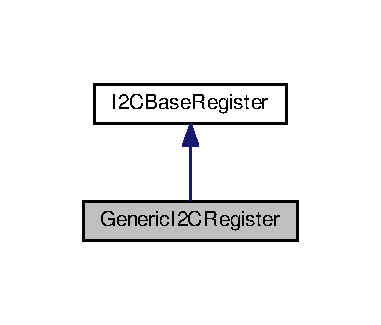
\includegraphics[width=183pt]{class_generic_i2_c_register__inherit__graph}
\end{center}
\end{figure}


Collaboration diagram for Generic\+I2\+C\+Register\+:
\nopagebreak
\begin{figure}[H]
\begin{center}
\leavevmode
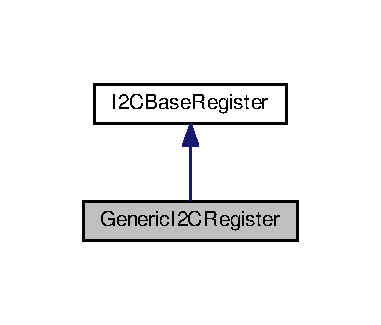
\includegraphics[width=183pt]{class_generic_i2_c_register__coll__graph}
\end{center}
\end{figure}
\subsection*{Public Member Functions}
\begin{DoxyCompactItemize}
\item 
\hyperlink{class_generic_i2_c_register_acc3dd8df2df5532b2e30ba20c1ac8735}{Generic\+I2\+C\+Register} (uint32\+\_\+t r, std\+::string rw, std\+::function$<$ \hyperlink{units__define_8hpp_a95d46867fa79633565c288a0b4bd5408}{units\+\_\+variant}(double value)$>$ read\+\_\+func, std\+::function$<$ uint8\+\_\+t(\hyperlink{units__define_8hpp_a95d46867fa79633565c288a0b4bd5408}{units\+\_\+variant})$>$ write\+\_\+func)
\begin{DoxyCompactList}\small\item\em Class constructor. \end{DoxyCompactList}\item 
\hyperlink{class_generic_i2_c_register_a17eb3844eb23aabe6fddfcef798e692f}{$\sim$\+Generic\+I2\+C\+Register} (void)
\begin{DoxyCompactList}\small\item\em Class destructor. \end{DoxyCompactList}\item 
\hyperlink{units__define_8hpp_a95d46867fa79633565c288a0b4bd5408}{units\+\_\+variant} \hyperlink{class_generic_i2_c_register_a86c28b9c5eecacca106132e7718b2646}{read} (\hyperlink{class_i2_c__base}{I2\+C\+\_\+base} $\ast$i2c\+\_\+ptr, uint32\+\_\+t address)
\begin{DoxyCompactList}\small\item\em Read data from register. \end{DoxyCompactList}\item 
void \hyperlink{class_generic_i2_c_register_ad6f38b7b54c95e3f8502de01f6122d60}{write} (\hyperlink{class_i2_c__base}{I2\+C\+\_\+base} $\ast$i2c\+\_\+ptr, uint32\+\_\+t address, \hyperlink{units__define_8hpp_a95d46867fa79633565c288a0b4bd5408}{units\+\_\+variant} value)
\begin{DoxyCompactList}\small\item\em Write data to register. \end{DoxyCompactList}\end{DoxyCompactItemize}
\subsection*{Additional Inherited Members}


\subsection{Detailed Description}
Derived \hyperlink{class_i2_c_base_register}{I2\+C\+Base\+Register} class for generic calls through lambda functions. Used when the interface is simple. 

Definition at line 33 of file I2\+C\+Register.\+hpp.



\subsection{Constructor \& Destructor Documentation}
\index{Generic\+I2\+C\+Register@{Generic\+I2\+C\+Register}!Generic\+I2\+C\+Register@{Generic\+I2\+C\+Register}}
\index{Generic\+I2\+C\+Register@{Generic\+I2\+C\+Register}!Generic\+I2\+C\+Register@{Generic\+I2\+C\+Register}}
\subsubsection[{\texorpdfstring{Generic\+I2\+C\+Register(uint32\+\_\+t r, std\+::string rw, std\+::function$<$ units\+\_\+variant(double value)$>$ read\+\_\+func, std\+::function$<$ uint8\+\_\+t(units\+\_\+variant)$>$ write\+\_\+func)}{GenericI2CRegister(uint32_t r, std::string rw, std::function< units_variant(double value)> read_func, std::function< uint8_t(units_variant)> write_func)}}]{\setlength{\rightskip}{0pt plus 5cm}Generic\+I2\+C\+Register\+::\+Generic\+I2\+C\+Register (
\begin{DoxyParamCaption}
\item[{uint32\+\_\+t}]{r, }
\item[{std\+::string}]{rw, }
\item[{std\+::function$<$ {\bf units\+\_\+variant}(double value)$>$}]{read\+\_\+func, }
\item[{std\+::function$<$ uint8\+\_\+t({\bf units\+\_\+variant})$>$}]{write\+\_\+func}
\end{DoxyParamCaption}
)}\hypertarget{class_generic_i2_c_register_acc3dd8df2df5532b2e30ba20c1ac8735}{}\label{class_generic_i2_c_register_acc3dd8df2df5532b2e30ba20c1ac8735}


Class constructor. 


\begin{DoxyParams}{Parameters}
{\em r} & -\/ Address of register within I2C device. \\
\hline
{\em read\+\_\+func} & -\/ Lambda function to convert hexadecimal value into correct units type. \\
\hline
{\em write\+\_\+func} & -\/ Lambda function to convert units type into uint8\+\_\+t to be written. \\
\hline
\end{DoxyParams}


Definition at line 16 of file I2\+C\+Register.\+cpp.

\index{Generic\+I2\+C\+Register@{Generic\+I2\+C\+Register}!````~Generic\+I2\+C\+Register@{$\sim$\+Generic\+I2\+C\+Register}}
\index{````~Generic\+I2\+C\+Register@{$\sim$\+Generic\+I2\+C\+Register}!Generic\+I2\+C\+Register@{Generic\+I2\+C\+Register}}
\subsubsection[{\texorpdfstring{$\sim$\+Generic\+I2\+C\+Register(void)}{~GenericI2CRegister(void)}}]{\setlength{\rightskip}{0pt plus 5cm}Generic\+I2\+C\+Register\+::$\sim$\+Generic\+I2\+C\+Register (
\begin{DoxyParamCaption}
\item[{void}]{}
\end{DoxyParamCaption}
)}\hypertarget{class_generic_i2_c_register_a17eb3844eb23aabe6fddfcef798e692f}{}\label{class_generic_i2_c_register_a17eb3844eb23aabe6fddfcef798e692f}


Class destructor. 



Definition at line 32 of file I2\+C\+Register.\+cpp.



\subsection{Member Function Documentation}
\index{Generic\+I2\+C\+Register@{Generic\+I2\+C\+Register}!read@{read}}
\index{read@{read}!Generic\+I2\+C\+Register@{Generic\+I2\+C\+Register}}
\subsubsection[{\texorpdfstring{read(\+I2\+C\+\_\+base $\ast$i2c\+\_\+ptr, uint32\+\_\+t address)}{read(I2C_base *i2c_ptr, uint32_t address)}}]{\setlength{\rightskip}{0pt plus 5cm}{\bf units\+\_\+variant} Generic\+I2\+C\+Register\+::read (
\begin{DoxyParamCaption}
\item[{{\bf I2\+C\+\_\+base} $\ast$}]{i2c\+\_\+ptr, }
\item[{uint32\+\_\+t}]{address}
\end{DoxyParamCaption}
)\hspace{0.3cm}{\ttfamily [virtual]}}\hypertarget{class_generic_i2_c_register_a86c28b9c5eecacca106132e7718b2646}{}\label{class_generic_i2_c_register_a86c28b9c5eecacca106132e7718b2646}


Read data from register. 


\begin{DoxyParams}{Parameters}
{\em i2c\+\_\+ptr} & -\/ Pointer to \hyperlink{class_i2_c__base}{I2\+C\+\_\+base} class used for transport. \\
\hline
\end{DoxyParams}
\begin{DoxyReturn}{Returns}
units\+\_\+variant containing quantity of correct type. 
\end{DoxyReturn}


Implements \hyperlink{class_i2_c_base_register_a947d834a745d3036c4cd8a2d5e19cd0d}{I2\+C\+Base\+Register}.



Definition at line 39 of file I2\+C\+Register.\+cpp.

\index{Generic\+I2\+C\+Register@{Generic\+I2\+C\+Register}!write@{write}}
\index{write@{write}!Generic\+I2\+C\+Register@{Generic\+I2\+C\+Register}}
\subsubsection[{\texorpdfstring{write(\+I2\+C\+\_\+base $\ast$i2c\+\_\+ptr, uint32\+\_\+t address, units\+\_\+variant value)}{write(I2C_base *i2c_ptr, uint32_t address, units_variant value)}}]{\setlength{\rightskip}{0pt plus 5cm}void Generic\+I2\+C\+Register\+::write (
\begin{DoxyParamCaption}
\item[{{\bf I2\+C\+\_\+base} $\ast$}]{i2c\+\_\+ptr, }
\item[{uint32\+\_\+t}]{address, }
\item[{{\bf units\+\_\+variant}}]{value}
\end{DoxyParamCaption}
)\hspace{0.3cm}{\ttfamily [virtual]}}\hypertarget{class_generic_i2_c_register_ad6f38b7b54c95e3f8502de01f6122d60}{}\label{class_generic_i2_c_register_ad6f38b7b54c95e3f8502de01f6122d60}


Write data to register. 


\begin{DoxyParams}{Parameters}
{\em i2c\+\_\+ptr} & -\/ Pointer to \hyperlink{class_i2_c__base}{I2\+C\+\_\+base} class used for transport. \\
\hline
{\em value} & -\/ Data to be written. Must be of correct type. \\
\hline
\end{DoxyParams}


Implements \hyperlink{class_i2_c_base_register_ad3f9f1404fe6af3e10e8f204b16d2066}{I2\+C\+Base\+Register}.



Definition at line 55 of file I2\+C\+Register.\+cpp.



The documentation for this class was generated from the following files\+:\begin{DoxyCompactItemize}
\item 
include/\hyperlink{_i2_c_register_8hpp}{I2\+C\+Register.\+hpp}\item 
src/\hyperlink{_i2_c_register_8cpp}{I2\+C\+Register.\+cpp}\end{DoxyCompactItemize}

\hypertarget{structnlohmann_1_1detail_1_1has__from__json}{}\section{nlohmann\+:\+:detail\+:\+:has\+\_\+from\+\_\+json$<$ Basic\+Json\+Type, T $>$ Struct Template Reference}
\label{structnlohmann_1_1detail_1_1has__from__json}\index{nlohmann\+::detail\+::has\+\_\+from\+\_\+json$<$ Basic\+Json\+Type, T $>$@{nlohmann\+::detail\+::has\+\_\+from\+\_\+json$<$ Basic\+Json\+Type, T $>$}}


{\ttfamily \#include $<$json.\+hpp$>$}

\subsection*{Static Public Attributes}
\begin{DoxyCompactItemize}
\item 
static constexpr bool \hyperlink{structnlohmann_1_1detail_1_1has__from__json_a16701d806343c58ae7e884024dd14955}{value}
\end{DoxyCompactItemize}


\subsection{Detailed Description}
\subsubsection*{template$<$typename Basic\+Json\+Type, typename T$>$\\*
struct nlohmann\+::detail\+::has\+\_\+from\+\_\+json$<$ Basic\+Json\+Type, T $>$}



Definition at line 810 of file json.\+hpp.



\subsection{Member Data Documentation}
\index{nlohmann\+::detail\+::has\+\_\+from\+\_\+json@{nlohmann\+::detail\+::has\+\_\+from\+\_\+json}!value@{value}}
\index{value@{value}!nlohmann\+::detail\+::has\+\_\+from\+\_\+json@{nlohmann\+::detail\+::has\+\_\+from\+\_\+json}}
\subsubsection[{\texorpdfstring{value}{value}}]{\setlength{\rightskip}{0pt plus 5cm}template$<$typename Basic\+Json\+Type , typename T $>$ constexpr bool {\bf nlohmann\+::detail\+::has\+\_\+from\+\_\+json}$<$ Basic\+Json\+Type, T $>$\+::value\hspace{0.3cm}{\ttfamily [static]}}\hypertarget{structnlohmann_1_1detail_1_1has__from__json_a16701d806343c58ae7e884024dd14955}{}\label{structnlohmann_1_1detail_1_1has__from__json_a16701d806343c58ae7e884024dd14955}
{\bfseries Initial value\+:}
\begin{DoxyCode}
= std::is\_integral<decltype(
                                      detect(std::declval<\textcolor{keyword}{typename} BasicJsonType::template 
      json\_serializer<T, void>>()))>\hyperlink{structnlohmann_1_1detail_1_1has__from__json_a16701d806343c58ae7e884024dd14955}{::value}
\end{DoxyCode}


Definition at line 820 of file json.\+hpp.



The documentation for this struct was generated from the following file\+:\begin{DoxyCompactItemize}
\item 
include/\hyperlink{json_8hpp}{json.\+hpp}\end{DoxyCompactItemize}

\hypertarget{structnlohmann_1_1detail_1_1has__non__default__from__json}{}\section{nlohmann\+:\+:detail\+:\+:has\+\_\+non\+\_\+default\+\_\+from\+\_\+json$<$ Basic\+Json\+Type, T $>$ Struct Template Reference}
\label{structnlohmann_1_1detail_1_1has__non__default__from__json}\index{nlohmann\+::detail\+::has\+\_\+non\+\_\+default\+\_\+from\+\_\+json$<$ Basic\+Json\+Type, T $>$@{nlohmann\+::detail\+::has\+\_\+non\+\_\+default\+\_\+from\+\_\+json$<$ Basic\+Json\+Type, T $>$}}


{\ttfamily \#include $<$json.\+hpp$>$}

\subsection*{Static Public Attributes}
\begin{DoxyCompactItemize}
\item 
static constexpr bool \hyperlink{structnlohmann_1_1detail_1_1has__non__default__from__json_ad34bb7cd3961fcafc2c5047a9782e931}{value}
\end{DoxyCompactItemize}


\subsection{Detailed Description}
\subsubsection*{template$<$typename Basic\+Json\+Type, typename T$>$\\*
struct nlohmann\+::detail\+::has\+\_\+non\+\_\+default\+\_\+from\+\_\+json$<$ Basic\+Json\+Type, T $>$}



Definition at line 827 of file json.\+hpp.



\subsection{Member Data Documentation}
\index{nlohmann\+::detail\+::has\+\_\+non\+\_\+default\+\_\+from\+\_\+json@{nlohmann\+::detail\+::has\+\_\+non\+\_\+default\+\_\+from\+\_\+json}!value@{value}}
\index{value@{value}!nlohmann\+::detail\+::has\+\_\+non\+\_\+default\+\_\+from\+\_\+json@{nlohmann\+::detail\+::has\+\_\+non\+\_\+default\+\_\+from\+\_\+json}}
\subsubsection[{\texorpdfstring{value}{value}}]{\setlength{\rightskip}{0pt plus 5cm}template$<$typename Basic\+Json\+Type , typename T $>$ constexpr bool {\bf nlohmann\+::detail\+::has\+\_\+non\+\_\+default\+\_\+from\+\_\+json}$<$ Basic\+Json\+Type, T $>$\+::value\hspace{0.3cm}{\ttfamily [static]}}\hypertarget{structnlohmann_1_1detail_1_1has__non__default__from__json_ad34bb7cd3961fcafc2c5047a9782e931}{}\label{structnlohmann_1_1detail_1_1has__non__default__from__json_ad34bb7cd3961fcafc2c5047a9782e931}
{\bfseries Initial value\+:}
\begin{DoxyCode}
= std::is\_integral<decltype(detect(
                                      std::declval<\textcolor{keyword}{typename} BasicJsonType::template json\_serializer<T,
       void>>()))>\hyperlink{structnlohmann_1_1detail_1_1has__non__default__from__json_ad34bb7cd3961fcafc2c5047a9782e931}{::value}
\end{DoxyCode}


Definition at line 838 of file json.\+hpp.



The documentation for this struct was generated from the following file\+:\begin{DoxyCompactItemize}
\item 
include/\hyperlink{json_8hpp}{json.\+hpp}\end{DoxyCompactItemize}

\hypertarget{structnlohmann_1_1detail_1_1has__to__json}{}\section{nlohmann\+:\+:detail\+:\+:has\+\_\+to\+\_\+json$<$ Basic\+Json\+Type, T $>$ Struct Template Reference}
\label{structnlohmann_1_1detail_1_1has__to__json}\index{nlohmann\+::detail\+::has\+\_\+to\+\_\+json$<$ Basic\+Json\+Type, T $>$@{nlohmann\+::detail\+::has\+\_\+to\+\_\+json$<$ Basic\+Json\+Type, T $>$}}


{\ttfamily \#include $<$json.\+hpp$>$}

\subsection*{Static Public Attributes}
\begin{DoxyCompactItemize}
\item 
static constexpr bool \hyperlink{structnlohmann_1_1detail_1_1has__to__json_a18e260c3c6f10328637c4427d3cb3a31}{value}
\end{DoxyCompactItemize}


\subsection{Detailed Description}
\subsubsection*{template$<$typename Basic\+Json\+Type, typename T$>$\\*
struct nlohmann\+::detail\+::has\+\_\+to\+\_\+json$<$ Basic\+Json\+Type, T $>$}



Definition at line 844 of file json.\+hpp.



\subsection{Member Data Documentation}
\index{nlohmann\+::detail\+::has\+\_\+to\+\_\+json@{nlohmann\+::detail\+::has\+\_\+to\+\_\+json}!value@{value}}
\index{value@{value}!nlohmann\+::detail\+::has\+\_\+to\+\_\+json@{nlohmann\+::detail\+::has\+\_\+to\+\_\+json}}
\subsubsection[{\texorpdfstring{value}{value}}]{\setlength{\rightskip}{0pt plus 5cm}template$<$typename Basic\+Json\+Type , typename T $>$ constexpr bool {\bf nlohmann\+::detail\+::has\+\_\+to\+\_\+json}$<$ Basic\+Json\+Type, T $>$\+::value\hspace{0.3cm}{\ttfamily [static]}}\hypertarget{structnlohmann_1_1detail_1_1has__to__json_a18e260c3c6f10328637c4427d3cb3a31}{}\label{structnlohmann_1_1detail_1_1has__to__json_a18e260c3c6f10328637c4427d3cb3a31}
{\bfseries Initial value\+:}
\begin{DoxyCode}
= std::is\_integral<decltype(detect(
                                      std::declval<\textcolor{keyword}{typename} BasicJsonType::template json\_serializer<T,
       void>>()))>\hyperlink{structnlohmann_1_1detail_1_1has__to__json_a18e260c3c6f10328637c4427d3cb3a31}{::value}
\end{DoxyCode}


Definition at line 853 of file json.\+hpp.



The documentation for this struct was generated from the following file\+:\begin{DoxyCompactItemize}
\item 
include/\hyperlink{json_8hpp}{json.\+hpp}\end{DoxyCompactItemize}

\hypertarget{structstd_1_1hash_3_01nlohmann_1_1json_01_4}{}\section{std\+:\+:hash$<$ nlohmann\+:\+:json $>$ Struct Template Reference}
\label{structstd_1_1hash_3_01nlohmann_1_1json_01_4}\index{std\+::hash$<$ nlohmann\+::json $>$@{std\+::hash$<$ nlohmann\+::json $>$}}


hash value for J\+S\+ON objects  




{\ttfamily \#include $<$json.\+hpp$>$}

\subsection*{Public Member Functions}
\begin{DoxyCompactItemize}
\item 
std\+::size\+\_\+t \hyperlink{structstd_1_1hash_3_01nlohmann_1_1json_01_4_afd03f6ad53db22868ca4163a8200b2f9}{operator()} (const \hyperlink{namespacenlohmann_a2bfd99e845a2e5cd90aeaf1b1431f474}{nlohmann\+::json} \&j) const 
\begin{DoxyCompactList}\small\item\em return a hash value for a J\+S\+ON object \end{DoxyCompactList}\end{DoxyCompactItemize}


\subsection{Detailed Description}
\subsubsection*{template$<$$>$\\*
struct std\+::hash$<$ nlohmann\+::json $>$}

hash value for J\+S\+ON objects 

Definition at line 14478 of file json.\+hpp.



\subsection{Member Function Documentation}
\index{std\+::hash$<$ nlohmann\+::json $>$@{std\+::hash$<$ nlohmann\+::json $>$}!operator()@{operator()}}
\index{operator()@{operator()}!std\+::hash$<$ nlohmann\+::json $>$@{std\+::hash$<$ nlohmann\+::json $>$}}
\subsubsection[{\texorpdfstring{operator()(const nlohmann\+::json \&j) const }{operator()(const nlohmann::json &j) const }}]{\setlength{\rightskip}{0pt plus 5cm}std\+::size\+\_\+t std\+::hash$<$ {\bf nlohmann\+::json} $>$\+::operator() (
\begin{DoxyParamCaption}
\item[{const {\bf nlohmann\+::json} \&}]{j}
\end{DoxyParamCaption}
) const\hspace{0.3cm}{\ttfamily [inline]}}\hypertarget{structstd_1_1hash_3_01nlohmann_1_1json_01_4_afd03f6ad53db22868ca4163a8200b2f9}{}\label{structstd_1_1hash_3_01nlohmann_1_1json_01_4_afd03f6ad53db22868ca4163a8200b2f9}


return a hash value for a J\+S\+ON object 

\begin{DoxySince}{Since}
version 1.\+0.\+0 
\end{DoxySince}


Definition at line 14485 of file json.\+hpp.



The documentation for this struct was generated from the following file\+:\begin{DoxyCompactItemize}
\item 
include/\hyperlink{json_8hpp}{json.\+hpp}\end{DoxyCompactItemize}

\hypertarget{class_i2_c__base}{}\section{I2\+C\+\_\+base Class Reference}
\label{class_i2_c__base}\index{I2\+C\+\_\+base@{I2\+C\+\_\+base}}


{\ttfamily \#include $<$I2\+C\+\_\+base.\+hpp$>$}



Inheritance diagram for I2\+C\+\_\+base\+:\nopagebreak
\begin{figure}[H]
\begin{center}
\leavevmode
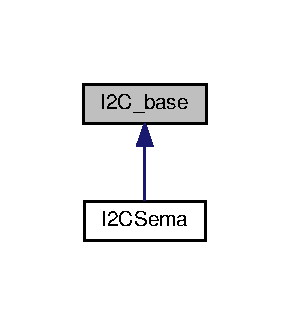
\includegraphics[width=139pt]{class_i2_c__base__inherit__graph}
\end{center}
\end{figure}
\subsection*{Public Member Functions}
\begin{DoxyCompactItemize}
\item 
virtual void \hyperlink{class_i2_c__base_a6938c7e851ac11836d2c69253ecd853a}{receive\+Data} (uint32\+\_\+t address, char $\ast$buffer, uint32\+\_\+t bytecnt, uint32\+\_\+t start\+\_\+point)=0
\item 
virtual void \hyperlink{class_i2_c__base_af78604423196f5b54602b08425c25622}{send\+Data} (uint32\+\_\+t address, char $\ast$buffer, uint32\+\_\+t bytecnt, uint32\+\_\+t start\+\_\+point)=0
\item 
virtual void \hyperlink{class_i2_c__base_a91e938610d77e20ae14e98861eb555c2}{get\+Board\+Value} (uint32\+\_\+t value, uint32\+\_\+t $\ast$buffer)=0
\end{DoxyCompactItemize}
\subsection*{Protected Attributes}
\begin{DoxyCompactItemize}
\item 
uint32\+\_\+t \hyperlink{class_i2_c__base_a49e4339d64cc99fcec489dea55c09e48}{addr}
\end{DoxyCompactItemize}


\subsection{Detailed Description}
Base I2C class. Has no functionality in current state but acts as a basis for derived I2C classes 

Definition at line 18 of file I2\+C\+\_\+base.\+hpp.



\subsection{Member Function Documentation}
\index{I2\+C\+\_\+base@{I2\+C\+\_\+base}!get\+Board\+Value@{get\+Board\+Value}}
\index{get\+Board\+Value@{get\+Board\+Value}!I2\+C\+\_\+base@{I2\+C\+\_\+base}}
\subsubsection[{\texorpdfstring{get\+Board\+Value(uint32\+\_\+t value, uint32\+\_\+t $\ast$buffer)=0}{getBoardValue(uint32_t value, uint32_t *buffer)=0}}]{\setlength{\rightskip}{0pt plus 5cm}virtual void I2\+C\+\_\+base\+::get\+Board\+Value (
\begin{DoxyParamCaption}
\item[{uint32\+\_\+t}]{value, }
\item[{uint32\+\_\+t $\ast$}]{buffer}
\end{DoxyParamCaption}
)\hspace{0.3cm}{\ttfamily [pure virtual]}}\hypertarget{class_i2_c__base_a91e938610d77e20ae14e98861eb555c2}{}\label{class_i2_c__base_a91e938610d77e20ae14e98861eb555c2}


Implemented in \hyperlink{class_i2_c_sema_ac03b06a86f07af407a1dbdc26a9b04c7}{I2\+C\+Sema}.

\index{I2\+C\+\_\+base@{I2\+C\+\_\+base}!receive\+Data@{receive\+Data}}
\index{receive\+Data@{receive\+Data}!I2\+C\+\_\+base@{I2\+C\+\_\+base}}
\subsubsection[{\texorpdfstring{receive\+Data(uint32\+\_\+t address, char $\ast$buffer, uint32\+\_\+t bytecnt, uint32\+\_\+t start\+\_\+point)=0}{receiveData(uint32_t address, char *buffer, uint32_t bytecnt, uint32_t start_point)=0}}]{\setlength{\rightskip}{0pt plus 5cm}virtual void I2\+C\+\_\+base\+::receive\+Data (
\begin{DoxyParamCaption}
\item[{uint32\+\_\+t}]{address, }
\item[{char $\ast$}]{buffer, }
\item[{uint32\+\_\+t}]{bytecnt, }
\item[{uint32\+\_\+t}]{start\+\_\+point}
\end{DoxyParamCaption}
)\hspace{0.3cm}{\ttfamily [pure virtual]}}\hypertarget{class_i2_c__base_a6938c7e851ac11836d2c69253ecd853a}{}\label{class_i2_c__base_a6938c7e851ac11836d2c69253ecd853a}


Implemented in \hyperlink{class_i2_c_sema_a6a30231be086ddee8255b8c9863a75fe}{I2\+C\+Sema}.

\index{I2\+C\+\_\+base@{I2\+C\+\_\+base}!send\+Data@{send\+Data}}
\index{send\+Data@{send\+Data}!I2\+C\+\_\+base@{I2\+C\+\_\+base}}
\subsubsection[{\texorpdfstring{send\+Data(uint32\+\_\+t address, char $\ast$buffer, uint32\+\_\+t bytecnt, uint32\+\_\+t start\+\_\+point)=0}{sendData(uint32_t address, char *buffer, uint32_t bytecnt, uint32_t start_point)=0}}]{\setlength{\rightskip}{0pt plus 5cm}virtual void I2\+C\+\_\+base\+::send\+Data (
\begin{DoxyParamCaption}
\item[{uint32\+\_\+t}]{address, }
\item[{char $\ast$}]{buffer, }
\item[{uint32\+\_\+t}]{bytecnt, }
\item[{uint32\+\_\+t}]{start\+\_\+point}
\end{DoxyParamCaption}
)\hspace{0.3cm}{\ttfamily [pure virtual]}}\hypertarget{class_i2_c__base_af78604423196f5b54602b08425c25622}{}\label{class_i2_c__base_af78604423196f5b54602b08425c25622}


Implemented in \hyperlink{class_i2_c_sema_a291907b6f7eca62b0d3957a19f86c239}{I2\+C\+Sema}.



\subsection{Member Data Documentation}
\index{I2\+C\+\_\+base@{I2\+C\+\_\+base}!addr@{addr}}
\index{addr@{addr}!I2\+C\+\_\+base@{I2\+C\+\_\+base}}
\subsubsection[{\texorpdfstring{addr}{addr}}]{\setlength{\rightskip}{0pt plus 5cm}uint32\+\_\+t I2\+C\+\_\+base\+::addr\hspace{0.3cm}{\ttfamily [protected]}}\hypertarget{class_i2_c__base_a49e4339d64cc99fcec489dea55c09e48}{}\label{class_i2_c__base_a49e4339d64cc99fcec489dea55c09e48}


Definition at line 20 of file I2\+C\+\_\+base.\+hpp.



The documentation for this class was generated from the following file\+:\begin{DoxyCompactItemize}
\item 
include/\hyperlink{_i2_c__base_8hpp}{I2\+C\+\_\+base.\+hpp}\end{DoxyCompactItemize}

\hypertarget{class_i2_c_base_register}{}\section{I2\+C\+Base\+Register Class Reference}
\label{class_i2_c_base_register}\index{I2\+C\+Base\+Register@{I2\+C\+Base\+Register}}


{\ttfamily \#include $<$I2\+C\+Register.\+hpp$>$}



Inheritance diagram for I2\+C\+Base\+Register\+:
\nopagebreak
\begin{figure}[H]
\begin{center}
\leavevmode
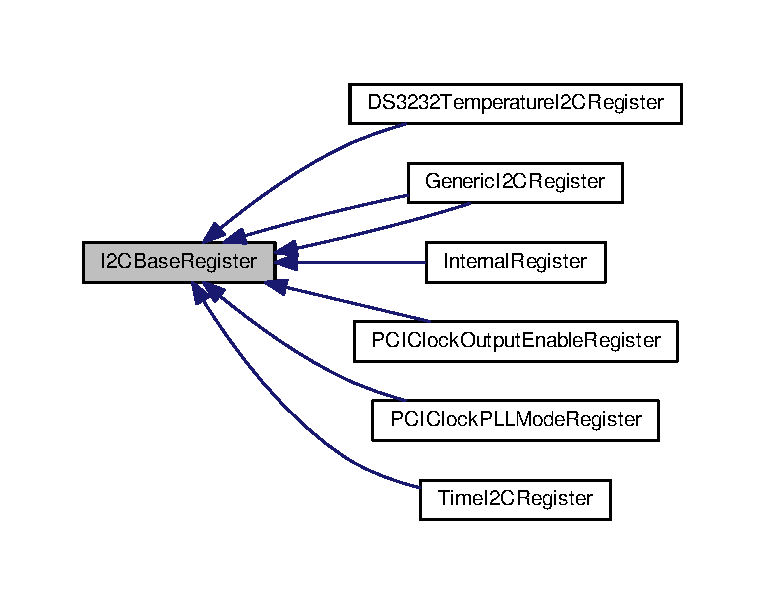
\includegraphics[width=350pt]{class_i2_c_base_register__inherit__graph}
\end{center}
\end{figure}
\subsection*{Public Member Functions}
\begin{DoxyCompactItemize}
\item 
virtual \hyperlink{units__define_8hpp_a95d46867fa79633565c288a0b4bd5408}{units\+\_\+variant} \hyperlink{class_i2_c_base_register_a947d834a745d3036c4cd8a2d5e19cd0d}{read} (\hyperlink{class_i2_c__base}{I2\+C\+\_\+base} $\ast$i2c\+\_\+ptr, uint32\+\_\+t address)=0
\item 
virtual void \hyperlink{class_i2_c_base_register_ad3f9f1404fe6af3e10e8f204b16d2066}{write} (\hyperlink{class_i2_c__base}{I2\+C\+\_\+base} $\ast$i2c\+\_\+ptr, uint32\+\_\+t address, \hyperlink{units__define_8hpp_a95d46867fa79633565c288a0b4bd5408}{units\+\_\+variant} value)=0
\end{DoxyCompactItemize}
\subsection*{Protected Attributes}
\begin{DoxyCompactItemize}
\item 
uint32\+\_\+t \hyperlink{class_i2_c_base_register_a5ec30e59be3ce0626848c665dbea8047}{reg}
\item 
bool \hyperlink{class_i2_c_base_register_a2e8f180fa393df31a1418d6f9cc55a1a}{b\+\_\+read}
\item 
bool \hyperlink{class_i2_c_base_register_ae0691af94ba363130da18520310a8c09}{b\+\_\+write}
\end{DoxyCompactItemize}


\subsection{Detailed Description}
I2\+C\+Register.\+h Purpose\+: defines \hyperlink{class_i2_c_base_register}{I2\+C\+Base\+Register} class and its derivations. \begin{DoxyAuthor}{Author}
David Monk 
\end{DoxyAuthor}
\begin{DoxyVersion}{Version}
1.\+0 Base class for I2C register is pure virtual and thus should not be constructed. 
\end{DoxyVersion}


Definition at line 19 of file I2\+C\+Register.\+hpp.



\subsection{Member Function Documentation}
\index{I2\+C\+Base\+Register@{I2\+C\+Base\+Register}!read@{read}}
\index{read@{read}!I2\+C\+Base\+Register@{I2\+C\+Base\+Register}}
\subsubsection[{\texorpdfstring{read(\+I2\+C\+\_\+base $\ast$i2c\+\_\+ptr, uint32\+\_\+t address)=0}{read(I2C_base *i2c_ptr, uint32_t address)=0}}]{\setlength{\rightskip}{0pt plus 5cm}virtual {\bf units\+\_\+variant} I2\+C\+Base\+Register\+::read (
\begin{DoxyParamCaption}
\item[{{\bf I2\+C\+\_\+base} $\ast$}]{i2c\+\_\+ptr, }
\item[{uint32\+\_\+t}]{address}
\end{DoxyParamCaption}
)\hspace{0.3cm}{\ttfamily [pure virtual]}}\hypertarget{class_i2_c_base_register_a947d834a745d3036c4cd8a2d5e19cd0d}{}\label{class_i2_c_base_register_a947d834a745d3036c4cd8a2d5e19cd0d}


Implemented in \hyperlink{class_internal_register_a7675a310cdb4866c256fef77d388b424}{Internal\+Register}, \hyperlink{class_p_c_i_clock_output_enable_register_a045c8a20c9ac76b937f7224aaba4a4ff}{P\+C\+I\+Clock\+Output\+Enable\+Register}, \hyperlink{class_p_c_i_clock_p_l_l_mode_register_afb680bb132c11af7c7f8ed5cba6a7150}{P\+C\+I\+Clock\+P\+L\+L\+Mode\+Register}, \hyperlink{class_d_s3232_temperature_i2_c_register_ab8733916ac8d733eb8d0e2b72df4efc2}{D\+S3232\+Temperature\+I2\+C\+Register}, \hyperlink{class_time_i2_c_register_a0b4f819644bed5adc645a089aec521da}{Time\+I2\+C\+Register}, and \hyperlink{class_generic_i2_c_register_a86c28b9c5eecacca106132e7718b2646}{Generic\+I2\+C\+Register}.

\index{I2\+C\+Base\+Register@{I2\+C\+Base\+Register}!write@{write}}
\index{write@{write}!I2\+C\+Base\+Register@{I2\+C\+Base\+Register}}
\subsubsection[{\texorpdfstring{write(\+I2\+C\+\_\+base $\ast$i2c\+\_\+ptr, uint32\+\_\+t address, units\+\_\+variant value)=0}{write(I2C_base *i2c_ptr, uint32_t address, units_variant value)=0}}]{\setlength{\rightskip}{0pt plus 5cm}virtual void I2\+C\+Base\+Register\+::write (
\begin{DoxyParamCaption}
\item[{{\bf I2\+C\+\_\+base} $\ast$}]{i2c\+\_\+ptr, }
\item[{uint32\+\_\+t}]{address, }
\item[{{\bf units\+\_\+variant}}]{value}
\end{DoxyParamCaption}
)\hspace{0.3cm}{\ttfamily [pure virtual]}}\hypertarget{class_i2_c_base_register_ad3f9f1404fe6af3e10e8f204b16d2066}{}\label{class_i2_c_base_register_ad3f9f1404fe6af3e10e8f204b16d2066}


Implemented in \hyperlink{class_internal_register_a8c1844d644fc81a118a6094f3a88feb8}{Internal\+Register}, \hyperlink{class_p_c_i_clock_output_enable_register_a85f345cbd4dac441680dbfebd20a15c0}{P\+C\+I\+Clock\+Output\+Enable\+Register}, \hyperlink{class_p_c_i_clock_p_l_l_mode_register_a19290b05f08da81c02cf34c9730f2b17}{P\+C\+I\+Clock\+P\+L\+L\+Mode\+Register}, \hyperlink{class_d_s3232_temperature_i2_c_register_a69c3e1c321d2161d8c69e984031d7fc8}{D\+S3232\+Temperature\+I2\+C\+Register}, \hyperlink{class_time_i2_c_register_a49301d14f0d10afa0f0ad7edeb6b30a7}{Time\+I2\+C\+Register}, and \hyperlink{class_generic_i2_c_register_ad6f38b7b54c95e3f8502de01f6122d60}{Generic\+I2\+C\+Register}.



\subsection{Member Data Documentation}
\index{I2\+C\+Base\+Register@{I2\+C\+Base\+Register}!b\+\_\+read@{b\+\_\+read}}
\index{b\+\_\+read@{b\+\_\+read}!I2\+C\+Base\+Register@{I2\+C\+Base\+Register}}
\subsubsection[{\texorpdfstring{b\+\_\+read}{b_read}}]{\setlength{\rightskip}{0pt plus 5cm}bool I2\+C\+Base\+Register\+::b\+\_\+read\hspace{0.3cm}{\ttfamily [protected]}}\hypertarget{class_i2_c_base_register_a2e8f180fa393df31a1418d6f9cc55a1a}{}\label{class_i2_c_base_register_a2e8f180fa393df31a1418d6f9cc55a1a}


Definition at line 22 of file I2\+C\+Register.\+hpp.

\index{I2\+C\+Base\+Register@{I2\+C\+Base\+Register}!b\+\_\+write@{b\+\_\+write}}
\index{b\+\_\+write@{b\+\_\+write}!I2\+C\+Base\+Register@{I2\+C\+Base\+Register}}
\subsubsection[{\texorpdfstring{b\+\_\+write}{b_write}}]{\setlength{\rightskip}{0pt plus 5cm}bool I2\+C\+Base\+Register\+::b\+\_\+write\hspace{0.3cm}{\ttfamily [protected]}}\hypertarget{class_i2_c_base_register_ae0691af94ba363130da18520310a8c09}{}\label{class_i2_c_base_register_ae0691af94ba363130da18520310a8c09}


Definition at line 23 of file I2\+C\+Register.\+hpp.

\index{I2\+C\+Base\+Register@{I2\+C\+Base\+Register}!reg@{reg}}
\index{reg@{reg}!I2\+C\+Base\+Register@{I2\+C\+Base\+Register}}
\subsubsection[{\texorpdfstring{reg}{reg}}]{\setlength{\rightskip}{0pt plus 5cm}uint32\+\_\+t I2\+C\+Base\+Register\+::reg\hspace{0.3cm}{\ttfamily [protected]}}\hypertarget{class_i2_c_base_register_a5ec30e59be3ce0626848c665dbea8047}{}\label{class_i2_c_base_register_a5ec30e59be3ce0626848c665dbea8047}


Definition at line 21 of file I2\+C\+Register.\+hpp.



The documentation for this class was generated from the following file\+:\begin{DoxyCompactItemize}
\item 
include/\hyperlink{_i2_c_register_8hpp}{I2\+C\+Register.\+hpp}\end{DoxyCompactItemize}

\hypertarget{class_i2_c_bus}{}\section{I2\+C\+Bus Class Reference}
\label{class_i2_c_bus}\index{I2\+C\+Bus@{I2\+C\+Bus}}


{\ttfamily \#include $<$I2\+C\+Bus.\+hpp$>$}

\subsection*{Public Member Functions}
\begin{DoxyCompactItemize}
\item 
\hyperlink{class_i2_c_bus_a53db5c5daff720905da00259e8ea5709}{I2\+C\+Bus} (std\+::unordered\+\_\+map$<$ std\+::string, \hyperlink{class_i2_c_device}{I2\+C\+Device} $\ast$ $>$ device\+\_\+map)
\begin{DoxyCompactList}\small\item\em Class constructor. \end{DoxyCompactList}\item 
\hyperlink{class_i2_c_bus_acdaf1b4ec82f6de308cc9604ce5e5e42}{$\sim$\+I2\+C\+Bus} (void)
\begin{DoxyCompactList}\small\item\em Class destructor. \end{DoxyCompactList}\item 
void \hyperlink{class_i2_c_bus_aeade1580d9ec9bba9a3b81f869b30243}{set\+Device} (std\+::string device\+\_\+id)
\begin{DoxyCompactList}\small\item\em Set device. \end{DoxyCompactList}\item 
void \hyperlink{class_i2_c_bus_a638333598e870191d42da15de6aeec0b}{set\+I2\+C\+Type} (\hyperlink{class_i2_c__base}{I2\+C\+\_\+base} $\ast$i2c\+\_\+type)
\begin{DoxyCompactList}\small\item\em Set I2C protocol to be used for communication. \end{DoxyCompactList}\item 
std\+::vector$<$ std\+::string $>$ \hyperlink{class_i2_c_bus_ab9cc5b3980240de9369ef6959881dd03}{get\+Properties} (void)
\begin{DoxyCompactList}\small\item\em Get properties of selected device. \end{DoxyCompactList}\item 
std\+::vector$<$ std\+::string $>$ \hyperlink{class_i2_c_bus_abddd1534dc9b08a0ed227af07b10fcab}{get\+Properties} (std\+::string device\+\_\+\+ID)
\begin{DoxyCompactList}\small\item\em Get properties of device. \end{DoxyCompactList}\item 
std\+::vector$<$ std\+::string $>$ \hyperlink{class_i2_c_bus_abff1e0e4b611c5a7d283c2e146b4281e}{get\+Devices} (void)
\begin{DoxyCompactList}\small\item\em Get devices on bus. \end{DoxyCompactList}\item 
\hyperlink{units__define_8hpp_a95d46867fa79633565c288a0b4bd5408}{units\+\_\+variant} \hyperlink{class_i2_c_bus_a9d933cda3071969110fcd5318a16e5ef}{read} (std\+::string property)
\begin{DoxyCompactList}\small\item\em Read property from device. \end{DoxyCompactList}\item 
void \hyperlink{class_i2_c_bus_aa3b0ce715377ed393d07916a4e75c2a9}{write} (std\+::string property, \hyperlink{units__define_8hpp_a95d46867fa79633565c288a0b4bd5408}{units\+\_\+variant} value)
\begin{DoxyCompactList}\small\item\em Write property to device. \end{DoxyCompactList}\end{DoxyCompactItemize}


\subsection{Detailed Description}


Definition at line 11 of file I2\+C\+Bus.\+hpp.



\subsection{Constructor \& Destructor Documentation}
\index{I2\+C\+Bus@{I2\+C\+Bus}!I2\+C\+Bus@{I2\+C\+Bus}}
\index{I2\+C\+Bus@{I2\+C\+Bus}!I2\+C\+Bus@{I2\+C\+Bus}}
\subsubsection[{\texorpdfstring{I2\+C\+Bus(std\+::unordered\+\_\+map$<$ std\+::string, I2\+C\+Device $\ast$ $>$ device\+\_\+map)}{I2CBus(std::unordered_map< std::string, I2CDevice * > device_map)}}]{\setlength{\rightskip}{0pt plus 5cm}I2\+C\+Bus\+::\+I2\+C\+Bus (
\begin{DoxyParamCaption}
\item[{std\+::unordered\+\_\+map$<$ std\+::string, {\bf I2\+C\+Device} $\ast$ $>$}]{device\+\_\+map}
\end{DoxyParamCaption}
)}\hypertarget{class_i2_c_bus_a53db5c5daff720905da00259e8ea5709}{}\label{class_i2_c_bus_a53db5c5daff720905da00259e8ea5709}


Class constructor. 


\begin{DoxyParams}{Parameters}
{\em device\+\_\+map} & -\/ Unordered map of string identifiers and \hyperlink{class_i2_c_device}{I2\+C\+Device} pointers. \\
\hline
\end{DoxyParams}


Definition at line 14 of file I2\+C\+Bus.\+cpp.

\index{I2\+C\+Bus@{I2\+C\+Bus}!````~I2\+C\+Bus@{$\sim$\+I2\+C\+Bus}}
\index{````~I2\+C\+Bus@{$\sim$\+I2\+C\+Bus}!I2\+C\+Bus@{I2\+C\+Bus}}
\subsubsection[{\texorpdfstring{$\sim$\+I2\+C\+Bus(void)}{~I2CBus(void)}}]{\setlength{\rightskip}{0pt plus 5cm}I2\+C\+Bus\+::$\sim$\+I2\+C\+Bus (
\begin{DoxyParamCaption}
\item[{void}]{}
\end{DoxyParamCaption}
)}\hypertarget{class_i2_c_bus_acdaf1b4ec82f6de308cc9604ce5e5e42}{}\label{class_i2_c_bus_acdaf1b4ec82f6de308cc9604ce5e5e42}


Class destructor. 



Definition at line 21 of file I2\+C\+Bus.\+cpp.



\subsection{Member Function Documentation}
\index{I2\+C\+Bus@{I2\+C\+Bus}!get\+Devices@{get\+Devices}}
\index{get\+Devices@{get\+Devices}!I2\+C\+Bus@{I2\+C\+Bus}}
\subsubsection[{\texorpdfstring{get\+Devices(void)}{getDevices(void)}}]{\setlength{\rightskip}{0pt plus 5cm}std\+::vector$<$ std\+::string $>$ I2\+C\+Bus\+::get\+Devices (
\begin{DoxyParamCaption}
\item[{void}]{}
\end{DoxyParamCaption}
)}\hypertarget{class_i2_c_bus_abff1e0e4b611c5a7d283c2e146b4281e}{}\label{class_i2_c_bus_abff1e0e4b611c5a7d283c2e146b4281e}


Get devices on bus. 

\begin{DoxyReturn}{Returns}
Vector of strings of each device ID. 
\end{DoxyReturn}


Definition at line 61 of file I2\+C\+Bus.\+cpp.

\index{I2\+C\+Bus@{I2\+C\+Bus}!get\+Properties@{get\+Properties}}
\index{get\+Properties@{get\+Properties}!I2\+C\+Bus@{I2\+C\+Bus}}
\subsubsection[{\texorpdfstring{get\+Properties(void)}{getProperties(void)}}]{\setlength{\rightskip}{0pt plus 5cm}std\+::vector$<$ std\+::string $>$ I2\+C\+Bus\+::get\+Properties (
\begin{DoxyParamCaption}
\item[{void}]{}
\end{DoxyParamCaption}
)}\hypertarget{class_i2_c_bus_ab9cc5b3980240de9369ef6959881dd03}{}\label{class_i2_c_bus_ab9cc5b3980240de9369ef6959881dd03}


Get properties of selected device. 

\begin{DoxyReturn}{Returns}
Vector of strings of each property for the selected device. 
\end{DoxyReturn}


Definition at line 43 of file I2\+C\+Bus.\+cpp.

\index{I2\+C\+Bus@{I2\+C\+Bus}!get\+Properties@{get\+Properties}}
\index{get\+Properties@{get\+Properties}!I2\+C\+Bus@{I2\+C\+Bus}}
\subsubsection[{\texorpdfstring{get\+Properties(std\+::string device\+\_\+\+I\+D)}{getProperties(std::string device_ID)}}]{\setlength{\rightskip}{0pt plus 5cm}std\+::vector$<$ std\+::string $>$ I2\+C\+Bus\+::get\+Properties (
\begin{DoxyParamCaption}
\item[{std\+::string}]{device\+\_\+\+ID}
\end{DoxyParamCaption}
)}\hypertarget{class_i2_c_bus_abddd1534dc9b08a0ed227af07b10fcab}{}\label{class_i2_c_bus_abddd1534dc9b08a0ed227af07b10fcab}


Get properties of device. 


\begin{DoxyParams}{Parameters}
{\em device} & -\/ String identifier for device. \\
\hline
\end{DoxyParams}
\begin{DoxyReturn}{Returns}
Vector of strings of each property for the device. 
\end{DoxyReturn}


Definition at line 52 of file I2\+C\+Bus.\+cpp.

\index{I2\+C\+Bus@{I2\+C\+Bus}!read@{read}}
\index{read@{read}!I2\+C\+Bus@{I2\+C\+Bus}}
\subsubsection[{\texorpdfstring{read(std\+::string property)}{read(std::string property)}}]{\setlength{\rightskip}{0pt plus 5cm}{\bf units\+\_\+variant} I2\+C\+Bus\+::read (
\begin{DoxyParamCaption}
\item[{std\+::string}]{property}
\end{DoxyParamCaption}
)}\hypertarget{class_i2_c_bus_a9d933cda3071969110fcd5318a16e5ef}{}\label{class_i2_c_bus_a9d933cda3071969110fcd5318a16e5ef}


Read property from device. 


\begin{DoxyParams}{Parameters}
{\em property} & -\/ String identifier for register to be read. \\
\hline
\end{DoxyParams}
\begin{DoxyReturn}{Returns}
units\+\_\+variant of value and associated unit. 
\end{DoxyReturn}


Definition at line 75 of file I2\+C\+Bus.\+cpp.

\index{I2\+C\+Bus@{I2\+C\+Bus}!set\+Device@{set\+Device}}
\index{set\+Device@{set\+Device}!I2\+C\+Bus@{I2\+C\+Bus}}
\subsubsection[{\texorpdfstring{set\+Device(std\+::string device\+\_\+id)}{setDevice(std::string device_id)}}]{\setlength{\rightskip}{0pt plus 5cm}void I2\+C\+Bus\+::set\+Device (
\begin{DoxyParamCaption}
\item[{std\+::string}]{device\+\_\+id}
\end{DoxyParamCaption}
)}\hypertarget{class_i2_c_bus_aeade1580d9ec9bba9a3b81f869b30243}{}\label{class_i2_c_bus_aeade1580d9ec9bba9a3b81f869b30243}


Set device. 


\begin{DoxyParams}{Parameters}
{\em device\+\_\+id} & -\/ String identifier of device. \\
\hline
\end{DoxyParams}


Definition at line 27 of file I2\+C\+Bus.\+cpp.

\index{I2\+C\+Bus@{I2\+C\+Bus}!set\+I2\+C\+Type@{set\+I2\+C\+Type}}
\index{set\+I2\+C\+Type@{set\+I2\+C\+Type}!I2\+C\+Bus@{I2\+C\+Bus}}
\subsubsection[{\texorpdfstring{set\+I2\+C\+Type(\+I2\+C\+\_\+base $\ast$i2c\+\_\+type)}{setI2CType(I2C_base *i2c_type)}}]{\setlength{\rightskip}{0pt plus 5cm}void I2\+C\+Bus\+::set\+I2\+C\+Type (
\begin{DoxyParamCaption}
\item[{{\bf I2\+C\+\_\+base} $\ast$}]{i2c\+\_\+type}
\end{DoxyParamCaption}
)}\hypertarget{class_i2_c_bus_a638333598e870191d42da15de6aeec0b}{}\label{class_i2_c_bus_a638333598e870191d42da15de6aeec0b}


Set I2C protocol to be used for communication. 


\begin{DoxyParams}{Parameters}
{\em i2c\+\_\+type} & -\/ \hyperlink{class_i2_c__base}{I2\+C\+\_\+base} pointer for transport object. \\
\hline
\end{DoxyParams}


Definition at line 35 of file I2\+C\+Bus.\+cpp.

\index{I2\+C\+Bus@{I2\+C\+Bus}!write@{write}}
\index{write@{write}!I2\+C\+Bus@{I2\+C\+Bus}}
\subsubsection[{\texorpdfstring{write(std\+::string property, units\+\_\+variant value)}{write(std::string property, units_variant value)}}]{\setlength{\rightskip}{0pt plus 5cm}void I2\+C\+Bus\+::write (
\begin{DoxyParamCaption}
\item[{std\+::string}]{property, }
\item[{{\bf units\+\_\+variant}}]{value}
\end{DoxyParamCaption}
)}\hypertarget{class_i2_c_bus_aa3b0ce715377ed393d07916a4e75c2a9}{}\label{class_i2_c_bus_aa3b0ce715377ed393d07916a4e75c2a9}


Write property to device. 


\begin{DoxyParams}{Parameters}
{\em property} & -\/ String identifier for register to be written to. \\
\hline
{\em units\+\_\+variant} & of value and associated unit to be written. \\
\hline
\end{DoxyParams}


Definition at line 84 of file I2\+C\+Bus.\+cpp.



The documentation for this class was generated from the following files\+:\begin{DoxyCompactItemize}
\item 
include/\hyperlink{_i2_c_bus_8hpp}{I2\+C\+Bus.\+hpp}\item 
src/\hyperlink{_i2_c_bus_8cpp}{I2\+C\+Bus.\+cpp}\end{DoxyCompactItemize}

\hypertarget{class_i2_c_device}{}\section{I2\+C\+Device Class Reference}
\label{class_i2_c_device}\index{I2\+C\+Device@{I2\+C\+Device}}


{\ttfamily \#include $<$I2\+C\+Device.\+hpp$>$}

\subsection*{Public Types}
\begin{DoxyCompactItemize}
\item 
enum \hyperlink{class_i2_c_device_a275eefb9eb7dfd1ee0470a8bd0a73086}{t\+I2\+Ctype} \{ \hyperlink{class_i2_c_device_a275eefb9eb7dfd1ee0470a8bd0a73086a6a7b9aebb5e9f27970de13799ad47f6e}{t\+I2\+Ctype\+::\+S\+E\+MA}, 
\hyperlink{class_i2_c_device_a275eefb9eb7dfd1ee0470a8bd0a73086a9a342381cd5923d1a59fdc8c22e286b7}{t\+I2\+Ctype\+::\+F\+T\+DI}, 
\hyperlink{class_i2_c_device_a275eefb9eb7dfd1ee0470a8bd0a73086a1fec00cf102e7c421f6662b56bd61fb7}{t\+I2\+Ctype\+::\+P\+C\+Ie}
 \}
\end{DoxyCompactItemize}
\subsection*{Public Member Functions}
\begin{DoxyCompactItemize}
\item 
\hyperlink{class_i2_c_device_a2e69a2e93dd5c82309f9e4983b3a9e74}{I2\+C\+Device} (uint32\+\_\+t addr, std\+::unordered\+\_\+map$<$ std\+::string, \hyperlink{class_i2_c_base_register}{I2\+C\+Base\+Register} $\ast$ $>$ reg\+\_\+map)
\begin{DoxyCompactList}\small\item\em Class constructor. \end{DoxyCompactList}\item 
\hyperlink{class_i2_c_device_a2edfce0d3f4d430f118fd6cc01483791}{I2\+C\+Device} (void)
\begin{DoxyCompactList}\small\item\em Default class constructor. \end{DoxyCompactList}\item 
\hyperlink{class_i2_c_device_a6d3bfa5e15112985958df9366589cdc5}{$\sim$\+I2\+C\+Device} (void)
\begin{DoxyCompactList}\small\item\em Class destructor. \end{DoxyCompactList}\item 
void \hyperlink{class_i2_c_device_aa12a7448f16100f8ed5d9a9903e94014}{set\+I2\+C\+Type} (\hyperlink{class_i2_c__base}{I2\+C\+\_\+base} $\ast$i2c\+\_\+type)
\item 
\hyperlink{units__define_8hpp_a95d46867fa79633565c288a0b4bd5408}{units\+\_\+variant} \hyperlink{class_i2_c_device_a402c8a5ecfc405e9a30d509118c19e7b}{read} (std\+::string reg)
\begin{DoxyCompactList}\small\item\em Read data from register. \end{DoxyCompactList}\item 
void \hyperlink{class_i2_c_device_a916d9450534684ea0260cacf94a0b79b}{write} (std\+::string reg, \hyperlink{units__define_8hpp_a95d46867fa79633565c288a0b4bd5408}{units\+\_\+variant} value)
\begin{DoxyCompactList}\small\item\em Write data to register. \end{DoxyCompactList}\item 
std\+::vector$<$ std\+::string $>$ \hyperlink{class_i2_c_device_a33e7d15ba04e33f8d61c23659037cb57}{get\+Properties} (void)
\begin{DoxyCompactList}\small\item\em Get all possible registers for given device. \end{DoxyCompactList}\end{DoxyCompactItemize}


\subsection{Detailed Description}
Class represents a single I2C device with a number of registers. Read/\+Write functions take a string-\/based ID for a given register. 

Definition at line 21 of file I2\+C\+Device.\+hpp.



\subsection{Member Enumeration Documentation}
\index{I2\+C\+Device@{I2\+C\+Device}!t\+I2\+Ctype@{t\+I2\+Ctype}}
\index{t\+I2\+Ctype@{t\+I2\+Ctype}!I2\+C\+Device@{I2\+C\+Device}}
\subsubsection[{\texorpdfstring{t\+I2\+Ctype}{tI2Ctype}}]{\setlength{\rightskip}{0pt plus 5cm}enum {\bf I2\+C\+Device\+::t\+I2\+Ctype}\hspace{0.3cm}{\ttfamily [strong]}}\hypertarget{class_i2_c_device_a275eefb9eb7dfd1ee0470a8bd0a73086}{}\label{class_i2_c_device_a275eefb9eb7dfd1ee0470a8bd0a73086}
\begin{Desc}
\item[Enumerator]\par
\begin{description}
\index{S\+E\+MA@{S\+E\+MA}!I2\+C\+Device@{I2\+C\+Device}}\index{I2\+C\+Device@{I2\+C\+Device}!S\+E\+MA@{S\+E\+MA}}\item[{\em 
S\+E\+MA\hypertarget{class_i2_c_device_a275eefb9eb7dfd1ee0470a8bd0a73086a6a7b9aebb5e9f27970de13799ad47f6e}{}\label{class_i2_c_device_a275eefb9eb7dfd1ee0470a8bd0a73086a6a7b9aebb5e9f27970de13799ad47f6e}
}]\index{F\+T\+DI@{F\+T\+DI}!I2\+C\+Device@{I2\+C\+Device}}\index{I2\+C\+Device@{I2\+C\+Device}!F\+T\+DI@{F\+T\+DI}}\item[{\em 
F\+T\+DI\hypertarget{class_i2_c_device_a275eefb9eb7dfd1ee0470a8bd0a73086a9a342381cd5923d1a59fdc8c22e286b7}{}\label{class_i2_c_device_a275eefb9eb7dfd1ee0470a8bd0a73086a9a342381cd5923d1a59fdc8c22e286b7}
}]\index{P\+C\+Ie@{P\+C\+Ie}!I2\+C\+Device@{I2\+C\+Device}}\index{I2\+C\+Device@{I2\+C\+Device}!P\+C\+Ie@{P\+C\+Ie}}\item[{\em 
P\+C\+Ie\hypertarget{class_i2_c_device_a275eefb9eb7dfd1ee0470a8bd0a73086a1fec00cf102e7c421f6662b56bd61fb7}{}\label{class_i2_c_device_a275eefb9eb7dfd1ee0470a8bd0a73086a1fec00cf102e7c421f6662b56bd61fb7}
}]\end{description}
\end{Desc}


Definition at line 28 of file I2\+C\+Device.\+hpp.



\subsection{Constructor \& Destructor Documentation}
\index{I2\+C\+Device@{I2\+C\+Device}!I2\+C\+Device@{I2\+C\+Device}}
\index{I2\+C\+Device@{I2\+C\+Device}!I2\+C\+Device@{I2\+C\+Device}}
\subsubsection[{\texorpdfstring{I2\+C\+Device(uint32\+\_\+t addr, std\+::unordered\+\_\+map$<$ std\+::string, I2\+C\+Base\+Register $\ast$ $>$ reg\+\_\+map)}{I2CDevice(uint32_t addr, std::unordered_map< std::string, I2CBaseRegister * > reg_map)}}]{\setlength{\rightskip}{0pt plus 5cm}I2\+C\+Device\+::\+I2\+C\+Device (
\begin{DoxyParamCaption}
\item[{uint32\+\_\+t}]{addr, }
\item[{std\+::unordered\+\_\+map$<$ std\+::string, {\bf I2\+C\+Base\+Register} $\ast$ $>$}]{reg\+\_\+map}
\end{DoxyParamCaption}
)}\hypertarget{class_i2_c_device_a2e69a2e93dd5c82309f9e4983b3a9e74}{}\label{class_i2_c_device_a2e69a2e93dd5c82309f9e4983b3a9e74}


Class constructor. 


\begin{DoxyParams}{Parameters}
{\em addr} & -\/ Address of device. \\
\hline
{\em reg\+\_\+map} & -\/ Unordered map of registers available on device. \\
\hline
\end{DoxyParams}


Definition at line 15 of file I2\+C\+Device.\+cpp.

\index{I2\+C\+Device@{I2\+C\+Device}!I2\+C\+Device@{I2\+C\+Device}}
\index{I2\+C\+Device@{I2\+C\+Device}!I2\+C\+Device@{I2\+C\+Device}}
\subsubsection[{\texorpdfstring{I2\+C\+Device(void)}{I2CDevice(void)}}]{\setlength{\rightskip}{0pt plus 5cm}I2\+C\+Device\+::\+I2\+C\+Device (
\begin{DoxyParamCaption}
\item[{void}]{}
\end{DoxyParamCaption}
)}\hypertarget{class_i2_c_device_a2edfce0d3f4d430f118fd6cc01483791}{}\label{class_i2_c_device_a2edfce0d3f4d430f118fd6cc01483791}


Default class constructor. 



Definition at line 23 of file I2\+C\+Device.\+cpp.

\index{I2\+C\+Device@{I2\+C\+Device}!````~I2\+C\+Device@{$\sim$\+I2\+C\+Device}}
\index{````~I2\+C\+Device@{$\sim$\+I2\+C\+Device}!I2\+C\+Device@{I2\+C\+Device}}
\subsubsection[{\texorpdfstring{$\sim$\+I2\+C\+Device(void)}{~I2CDevice(void)}}]{\setlength{\rightskip}{0pt plus 5cm}I2\+C\+Device\+::$\sim$\+I2\+C\+Device (
\begin{DoxyParamCaption}
\item[{void}]{}
\end{DoxyParamCaption}
)}\hypertarget{class_i2_c_device_a6d3bfa5e15112985958df9366589cdc5}{}\label{class_i2_c_device_a6d3bfa5e15112985958df9366589cdc5}


Class destructor. 



Definition at line 32 of file I2\+C\+Device.\+cpp.



\subsection{Member Function Documentation}
\index{I2\+C\+Device@{I2\+C\+Device}!get\+Properties@{get\+Properties}}
\index{get\+Properties@{get\+Properties}!I2\+C\+Device@{I2\+C\+Device}}
\subsubsection[{\texorpdfstring{get\+Properties(void)}{getProperties(void)}}]{\setlength{\rightskip}{0pt plus 5cm}std\+::vector$<$ std\+::string $>$ I2\+C\+Device\+::get\+Properties (
\begin{DoxyParamCaption}
\item[{void}]{}
\end{DoxyParamCaption}
)}\hypertarget{class_i2_c_device_a33e7d15ba04e33f8d61c23659037cb57}{}\label{class_i2_c_device_a33e7d15ba04e33f8d61c23659037cb57}


Get all possible registers for given device. 

\begin{DoxyReturn}{Returns}
Vector of strings assosciated with the properties. 
\end{DoxyReturn}


Definition at line 58 of file I2\+C\+Device.\+cpp.

\index{I2\+C\+Device@{I2\+C\+Device}!read@{read}}
\index{read@{read}!I2\+C\+Device@{I2\+C\+Device}}
\subsubsection[{\texorpdfstring{read(std\+::string reg)}{read(std::string reg)}}]{\setlength{\rightskip}{0pt plus 5cm}{\bf units\+\_\+variant} I2\+C\+Device\+::read (
\begin{DoxyParamCaption}
\item[{std\+::string}]{reg}
\end{DoxyParamCaption}
)}\hypertarget{class_i2_c_device_a402c8a5ecfc405e9a30d509118c19e7b}{}\label{class_i2_c_device_a402c8a5ecfc405e9a30d509118c19e7b}


Read data from register. 


\begin{DoxyParams}{Parameters}
{\em reg} & -\/ Property to read. \\
\hline
\end{DoxyParams}
\begin{DoxyReturn}{Returns}
units\+\_\+variant containing quantity of correct type. 
\end{DoxyReturn}


Definition at line 39 of file I2\+C\+Device.\+cpp.

\index{I2\+C\+Device@{I2\+C\+Device}!set\+I2\+C\+Type@{set\+I2\+C\+Type}}
\index{set\+I2\+C\+Type@{set\+I2\+C\+Type}!I2\+C\+Device@{I2\+C\+Device}}
\subsubsection[{\texorpdfstring{set\+I2\+C\+Type(\+I2\+C\+\_\+base $\ast$i2c\+\_\+type)}{setI2CType(I2C_base *i2c_type)}}]{\setlength{\rightskip}{0pt plus 5cm}void I2\+C\+Device\+::set\+I2\+C\+Type (
\begin{DoxyParamCaption}
\item[{{\bf I2\+C\+\_\+base} $\ast$}]{i2c\+\_\+type}
\end{DoxyParamCaption}
)}\hypertarget{class_i2_c_device_aa12a7448f16100f8ed5d9a9903e94014}{}\label{class_i2_c_device_aa12a7448f16100f8ed5d9a9903e94014}


Definition at line 25 of file I2\+C\+Device.\+cpp.

\index{I2\+C\+Device@{I2\+C\+Device}!write@{write}}
\index{write@{write}!I2\+C\+Device@{I2\+C\+Device}}
\subsubsection[{\texorpdfstring{write(std\+::string reg, units\+\_\+variant value)}{write(std::string reg, units_variant value)}}]{\setlength{\rightskip}{0pt plus 5cm}void I2\+C\+Device\+::write (
\begin{DoxyParamCaption}
\item[{std\+::string}]{reg, }
\item[{{\bf units\+\_\+variant}}]{value}
\end{DoxyParamCaption}
)}\hypertarget{class_i2_c_device_a916d9450534684ea0260cacf94a0b79b}{}\label{class_i2_c_device_a916d9450534684ea0260cacf94a0b79b}


Write data to register. 


\begin{DoxyParams}{Parameters}
{\em reg} & -\/ Property to write to. \\
\hline
{\em value} & -\/ Data to write to register. Must be of the correct type. \\
\hline
\end{DoxyParams}


Definition at line 49 of file I2\+C\+Device.\+cpp.



The documentation for this class was generated from the following files\+:\begin{DoxyCompactItemize}
\item 
include/\hyperlink{_i2_c_device_8hpp}{I2\+C\+Device.\+hpp}\item 
src/\hyperlink{_i2_c_device_8cpp}{I2\+C\+Device.\+cpp}\end{DoxyCompactItemize}

\hypertarget{class_i2_c_raw}{}\section{I2\+C\+Raw Class Reference}
\label{class_i2_c_raw}\index{I2\+C\+Raw@{I2\+C\+Raw}}


{\ttfamily \#include $<$I2\+C\+Raw.\+hpp$>$}

\subsection*{Public Member Functions}
\begin{DoxyCompactItemize}
\item 
\hyperlink{class_i2_c_raw_a8df65f9a9dc54dbc75205594a2d9b9f7}{I2\+C\+Raw} (void)
\begin{DoxyCompactList}\small\item\em Class constructor. \end{DoxyCompactList}\item 
\hyperlink{class_i2_c_raw_a9e5a7ede7b48487b67d7020d609a6ae6}{$\sim$\+I2\+C\+Raw} ()
\begin{DoxyCompactList}\small\item\em Class destructor. \end{DoxyCompactList}\item 
int \hyperlink{class_i2_c_raw_a35dd63654acfea8ddd46fddbcae8569b}{read} (uint32\+\_\+t address, uint32\+\_\+t start\+\_\+point)
\begin{DoxyCompactList}\small\item\em Read from register. \end{DoxyCompactList}\item 
void \hyperlink{class_i2_c_raw_a0e7b8c5f728e0805bb31c20fdbd77a33}{write} (uint32\+\_\+t address, uint8\+\_\+t buffer, uint32\+\_\+t start\+\_\+point)
\begin{DoxyCompactList}\small\item\em Write to register. \end{DoxyCompactList}\end{DoxyCompactItemize}


\subsection{Detailed Description}


Definition at line 11 of file I2\+C\+Raw.\+hpp.



\subsection{Constructor \& Destructor Documentation}
\index{I2\+C\+Raw@{I2\+C\+Raw}!I2\+C\+Raw@{I2\+C\+Raw}}
\index{I2\+C\+Raw@{I2\+C\+Raw}!I2\+C\+Raw@{I2\+C\+Raw}}
\subsubsection[{\texorpdfstring{I2\+C\+Raw(void)}{I2CRaw(void)}}]{\setlength{\rightskip}{0pt plus 5cm}I2\+C\+Raw\+::\+I2\+C\+Raw (
\begin{DoxyParamCaption}
\item[{void}]{}
\end{DoxyParamCaption}
)}\hypertarget{class_i2_c_raw_a8df65f9a9dc54dbc75205594a2d9b9f7}{}\label{class_i2_c_raw_a8df65f9a9dc54dbc75205594a2d9b9f7}


Class constructor. 



Definition at line 13 of file I2\+C\+Raw.\+cpp.

\index{I2\+C\+Raw@{I2\+C\+Raw}!````~I2\+C\+Raw@{$\sim$\+I2\+C\+Raw}}
\index{````~I2\+C\+Raw@{$\sim$\+I2\+C\+Raw}!I2\+C\+Raw@{I2\+C\+Raw}}
\subsubsection[{\texorpdfstring{$\sim$\+I2\+C\+Raw()}{~I2CRaw()}}]{\setlength{\rightskip}{0pt plus 5cm}I2\+C\+Raw\+::$\sim$\+I2\+C\+Raw (
\begin{DoxyParamCaption}
{}
\end{DoxyParamCaption}
)}\hypertarget{class_i2_c_raw_a9e5a7ede7b48487b67d7020d609a6ae6}{}\label{class_i2_c_raw_a9e5a7ede7b48487b67d7020d609a6ae6}


Class destructor. 



Definition at line 22 of file I2\+C\+Raw.\+cpp.



\subsection{Member Function Documentation}
\index{I2\+C\+Raw@{I2\+C\+Raw}!read@{read}}
\index{read@{read}!I2\+C\+Raw@{I2\+C\+Raw}}
\subsubsection[{\texorpdfstring{read(uint32\+\_\+t address, uint32\+\_\+t start\+\_\+point)}{read(uint32_t address, uint32_t start_point)}}]{\setlength{\rightskip}{0pt plus 5cm}int I2\+C\+Raw\+::read (
\begin{DoxyParamCaption}
\item[{uint32\+\_\+t}]{address, }
\item[{uint32\+\_\+t}]{start\+\_\+point}
\end{DoxyParamCaption}
)}\hypertarget{class_i2_c_raw_a35dd63654acfea8ddd46fddbcae8569b}{}\label{class_i2_c_raw_a35dd63654acfea8ddd46fddbcae8569b}


Read from register. 


\begin{DoxyParams}{Parameters}
{\em address} & -\/ Device address. \\
\hline
{\em start\+\_\+point} & -\/ Internal register address \\
\hline
\end{DoxyParams}
\begin{DoxyReturn}{Returns}
Integer representation of hex output. 
\end{DoxyReturn}


Definition at line 73 of file I2\+C\+Raw.\+cpp.

\index{I2\+C\+Raw@{I2\+C\+Raw}!write@{write}}
\index{write@{write}!I2\+C\+Raw@{I2\+C\+Raw}}
\subsubsection[{\texorpdfstring{write(uint32\+\_\+t address, uint8\+\_\+t buffer, uint32\+\_\+t start\+\_\+point)}{write(uint32_t address, uint8_t buffer, uint32_t start_point)}}]{\setlength{\rightskip}{0pt plus 5cm}void I2\+C\+Raw\+::write (
\begin{DoxyParamCaption}
\item[{uint32\+\_\+t}]{address, }
\item[{uint8\+\_\+t}]{buffer, }
\item[{uint32\+\_\+t}]{start\+\_\+point}
\end{DoxyParamCaption}
)}\hypertarget{class_i2_c_raw_a0e7b8c5f728e0805bb31c20fdbd77a33}{}\label{class_i2_c_raw_a0e7b8c5f728e0805bb31c20fdbd77a33}


Write to register. 


\begin{DoxyParams}{Parameters}
{\em address} & -\/ Device address. \\
\hline
{\em buffer} & -\/ Data to be written to register. \\
\hline
{\em start\+\_\+point} & -\/ Internal register address \\
\hline
\end{DoxyParams}


Definition at line 84 of file I2\+C\+Raw.\+cpp.



The documentation for this class was generated from the following files\+:\begin{DoxyCompactItemize}
\item 
include/\hyperlink{_i2_c_raw_8hpp}{I2\+C\+Raw.\+hpp}\item 
src/\hyperlink{_i2_c_raw_8cpp}{I2\+C\+Raw.\+cpp}\end{DoxyCompactItemize}

\hypertarget{class_i2_c_sema}{}\section{I2\+C\+Sema Class Reference}
\label{class_i2_c_sema}\index{I2\+C\+Sema@{I2\+C\+Sema}}


{\ttfamily \#include $<$I2\+C.\+hpp$>$}



Inheritance diagram for I2\+C\+Sema\+:\nopagebreak
\begin{figure}[H]
\begin{center}
\leavevmode
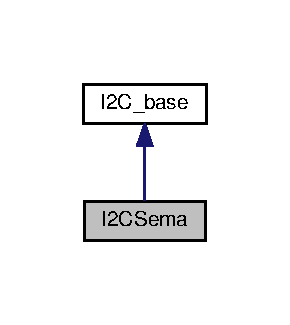
\includegraphics[width=139pt]{class_i2_c_sema__inherit__graph}
\end{center}
\end{figure}


Collaboration diagram for I2\+C\+Sema\+:\nopagebreak
\begin{figure}[H]
\begin{center}
\leavevmode
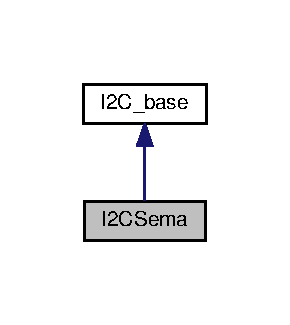
\includegraphics[width=139pt]{class_i2_c_sema__coll__graph}
\end{center}
\end{figure}
\subsection*{Public Member Functions}
\begin{DoxyCompactItemize}
\item 
\hyperlink{class_i2_c_sema_ad9b53f523e31c4a24a73463591473358}{I2\+C\+Sema} (uint32\+\_\+t ID, uint32\+\_\+t address, bool diag)
\begin{DoxyCompactList}\small\item\em Constructor function with additional diagnostics. \end{DoxyCompactList}\item 
\hyperlink{class_i2_c_sema_a627eb561a9ca1bb08f39a4f58cae0b3c}{I2\+C\+Sema} (uint32\+\_\+t ID)
\begin{DoxyCompactList}\small\item\em Constructor function. \end{DoxyCompactList}\item 
\hyperlink{class_i2_c_sema_ade6cfd73c317f5339a5b02558b5f5a11}{$\sim$\+I2\+C\+Sema} (void)
\begin{DoxyCompactList}\small\item\em Class destructor. \end{DoxyCompactList}\item 
uint32\+\_\+t \hyperlink{class_i2_c_sema_ad4d4a853db59af3579b29dbc1b739406}{get\+Bus\+Cap} (void)
\begin{DoxyCompactList}\small\item\em Get the maximum block length for given I2C bus ID. \end{DoxyCompactList}\item 
void \hyperlink{class_i2_c_sema_a6a30231be086ddee8255b8c9863a75fe}{receive\+Data} (uint32\+\_\+t address, char $\ast$buffer, uint32\+\_\+t bytecnt, uint32\+\_\+t start\+\_\+point)
\begin{DoxyCompactList}\small\item\em Receive data data from addressed slave. \end{DoxyCompactList}\item 
void \hyperlink{class_i2_c_sema_a291907b6f7eca62b0d3957a19f86c239}{send\+Data} (uint32\+\_\+t address, char $\ast$buffer, uint32\+\_\+t bytecnt, uint32\+\_\+t start\+\_\+point)
\begin{DoxyCompactList}\small\item\em Send data data to addressed slave. \end{DoxyCompactList}\item 
void \hyperlink{class_i2_c_sema_ac03b06a86f07af407a1dbdc26a9b04c7}{get\+Board\+Value} (uint32\+\_\+t value, uint32\+\_\+t $\ast$buffer)
\begin{DoxyCompactList}\small\item\em Get value from board registers. \end{DoxyCompactList}\end{DoxyCompactItemize}
\subsection*{Additional Inherited Members}


\subsection{Detailed Description}
Derived class from I2C which implements S\+E\+MA A\+PI function calls to communicate with bus. 

Definition at line 20 of file I2\+C.\+hpp.



\subsection{Constructor \& Destructor Documentation}
\index{I2\+C\+Sema@{I2\+C\+Sema}!I2\+C\+Sema@{I2\+C\+Sema}}
\index{I2\+C\+Sema@{I2\+C\+Sema}!I2\+C\+Sema@{I2\+C\+Sema}}
\subsubsection[{\texorpdfstring{I2\+C\+Sema(uint32\+\_\+t I\+D, uint32\+\_\+t address, bool diag)}{I2CSema(uint32_t ID, uint32_t address, bool diag)}}]{\setlength{\rightskip}{0pt plus 5cm}I2\+C\+Sema\+::\+I2\+C\+Sema (
\begin{DoxyParamCaption}
\item[{uint32\+\_\+t}]{ID, }
\item[{uint32\+\_\+t}]{address, }
\item[{bool}]{diag}
\end{DoxyParamCaption}
)}\hypertarget{class_i2_c_sema_ad9b53f523e31c4a24a73463591473358}{}\label{class_i2_c_sema_ad9b53f523e31c4a24a73463591473358}


Constructor function with additional diagnostics. 


\begin{DoxyParams}{Parameters}
{\em ID} & -\/ I2C bus ID. \\
\hline
{\em address} & -\/ Address of slave module. \\
\hline
{\em diag} & -\/ Set to true to display diagnostics. \\
\hline
\end{DoxyParams}


Definition at line 33 of file I2\+C.\+cpp.

\index{I2\+C\+Sema@{I2\+C\+Sema}!I2\+C\+Sema@{I2\+C\+Sema}}
\index{I2\+C\+Sema@{I2\+C\+Sema}!I2\+C\+Sema@{I2\+C\+Sema}}
\subsubsection[{\texorpdfstring{I2\+C\+Sema(uint32\+\_\+t I\+D)}{I2CSema(uint32_t ID)}}]{\setlength{\rightskip}{0pt plus 5cm}I2\+C\+Sema\+::\+I2\+C\+Sema (
\begin{DoxyParamCaption}
\item[{uint32\+\_\+t}]{ID}
\end{DoxyParamCaption}
)}\hypertarget{class_i2_c_sema_a627eb561a9ca1bb08f39a4f58cae0b3c}{}\label{class_i2_c_sema_a627eb561a9ca1bb08f39a4f58cae0b3c}


Constructor function. 


\begin{DoxyParams}{Parameters}
{\em ID} & -\/ I2C bus ID. \\
\hline
{\em address} & -\/ Address of slave module. \\
\hline
\end{DoxyParams}


Definition at line 15 of file I2\+C.\+cpp.

\index{I2\+C\+Sema@{I2\+C\+Sema}!````~I2\+C\+Sema@{$\sim$\+I2\+C\+Sema}}
\index{````~I2\+C\+Sema@{$\sim$\+I2\+C\+Sema}!I2\+C\+Sema@{I2\+C\+Sema}}
\subsubsection[{\texorpdfstring{$\sim$\+I2\+C\+Sema(void)}{~I2CSema(void)}}]{\setlength{\rightskip}{0pt plus 5cm}I2\+C\+Sema\+::$\sim$\+I2\+C\+Sema (
\begin{DoxyParamCaption}
\item[{void}]{}
\end{DoxyParamCaption}
)}\hypertarget{class_i2_c_sema_ade6cfd73c317f5339a5b02558b5f5a11}{}\label{class_i2_c_sema_ade6cfd73c317f5339a5b02558b5f5a11}


Class destructor. 



Definition at line 56 of file I2\+C.\+cpp.



\subsection{Member Function Documentation}
\index{I2\+C\+Sema@{I2\+C\+Sema}!get\+Board\+Value@{get\+Board\+Value}}
\index{get\+Board\+Value@{get\+Board\+Value}!I2\+C\+Sema@{I2\+C\+Sema}}
\subsubsection[{\texorpdfstring{get\+Board\+Value(uint32\+\_\+t value, uint32\+\_\+t $\ast$buffer)}{getBoardValue(uint32_t value, uint32_t *buffer)}}]{\setlength{\rightskip}{0pt plus 5cm}void I2\+C\+Sema\+::get\+Board\+Value (
\begin{DoxyParamCaption}
\item[{uint32\+\_\+t}]{value, }
\item[{uint32\+\_\+t $\ast$}]{buffer}
\end{DoxyParamCaption}
)\hspace{0.3cm}{\ttfamily [virtual]}}\hypertarget{class_i2_c_sema_ac03b06a86f07af407a1dbdc26a9b04c7}{}\label{class_i2_c_sema_ac03b06a86f07af407a1dbdc26a9b04c7}


Get value from board registers. 


\begin{DoxyParams}{Parameters}
{\em value} & -\/ ID of internal regiter to read. \\
\hline
{\em buffer} & -\/ Pointer to byte array where data will be sent from. \\
\hline
\end{DoxyParams}


Implements \hyperlink{class_i2_c__base_a91e938610d77e20ae14e98861eb555c2}{I2\+C\+\_\+base}.



Definition at line 113 of file I2\+C.\+cpp.

\index{I2\+C\+Sema@{I2\+C\+Sema}!get\+Bus\+Cap@{get\+Bus\+Cap}}
\index{get\+Bus\+Cap@{get\+Bus\+Cap}!I2\+C\+Sema@{I2\+C\+Sema}}
\subsubsection[{\texorpdfstring{get\+Bus\+Cap(void)}{getBusCap(void)}}]{\setlength{\rightskip}{0pt plus 5cm}uint32\+\_\+t I2\+C\+Sema\+::get\+Bus\+Cap (
\begin{DoxyParamCaption}
\item[{void}]{}
\end{DoxyParamCaption}
)}\hypertarget{class_i2_c_sema_ad4d4a853db59af3579b29dbc1b739406}{}\label{class_i2_c_sema_ad4d4a853db59af3579b29dbc1b739406}


Get the maximum block length for given I2C bus ID. 

\begin{DoxyReturn}{Returns}
Block length as integer. 
\end{DoxyReturn}


Definition at line 64 of file I2\+C.\+cpp.

\index{I2\+C\+Sema@{I2\+C\+Sema}!receive\+Data@{receive\+Data}}
\index{receive\+Data@{receive\+Data}!I2\+C\+Sema@{I2\+C\+Sema}}
\subsubsection[{\texorpdfstring{receive\+Data(uint32\+\_\+t address, char $\ast$buffer, uint32\+\_\+t bytecnt, uint32\+\_\+t start\+\_\+point)}{receiveData(uint32_t address, char *buffer, uint32_t bytecnt, uint32_t start_point)}}]{\setlength{\rightskip}{0pt plus 5cm}void I2\+C\+Sema\+::receive\+Data (
\begin{DoxyParamCaption}
\item[{uint32\+\_\+t}]{address, }
\item[{char $\ast$}]{buffer, }
\item[{uint32\+\_\+t}]{bytecnt, }
\item[{uint32\+\_\+t}]{start\+\_\+point}
\end{DoxyParamCaption}
)\hspace{0.3cm}{\ttfamily [virtual]}}\hypertarget{class_i2_c_sema_a6a30231be086ddee8255b8c9863a75fe}{}\label{class_i2_c_sema_a6a30231be086ddee8255b8c9863a75fe}


Receive data data from addressed slave. 


\begin{DoxyParams}{Parameters}
{\em buffer} & -\/ Pointer to byte array where data will be written. \\
\hline
{\em bytecnt} & -\/ Length of buffer. \\
\hline
{\em start\+\_\+point} & -\/ Starting address within slave. \\
\hline
\end{DoxyParams}
\begin{DoxyReturn}{Returns}
Pointer to array where data was written. 
\end{DoxyReturn}


Implements \hyperlink{class_i2_c__base_a6938c7e851ac11836d2c69253ecd853a}{I2\+C\+\_\+base}.



Definition at line 83 of file I2\+C.\+cpp.

\index{I2\+C\+Sema@{I2\+C\+Sema}!send\+Data@{send\+Data}}
\index{send\+Data@{send\+Data}!I2\+C\+Sema@{I2\+C\+Sema}}
\subsubsection[{\texorpdfstring{send\+Data(uint32\+\_\+t address, char $\ast$buffer, uint32\+\_\+t bytecnt, uint32\+\_\+t start\+\_\+point)}{sendData(uint32_t address, char *buffer, uint32_t bytecnt, uint32_t start_point)}}]{\setlength{\rightskip}{0pt plus 5cm}void I2\+C\+Sema\+::send\+Data (
\begin{DoxyParamCaption}
\item[{uint32\+\_\+t}]{address, }
\item[{char $\ast$}]{buffer, }
\item[{uint32\+\_\+t}]{bytecnt, }
\item[{uint32\+\_\+t}]{start\+\_\+point}
\end{DoxyParamCaption}
)\hspace{0.3cm}{\ttfamily [virtual]}}\hypertarget{class_i2_c_sema_a291907b6f7eca62b0d3957a19f86c239}{}\label{class_i2_c_sema_a291907b6f7eca62b0d3957a19f86c239}


Send data data to addressed slave. 


\begin{DoxyParams}{Parameters}
{\em buffer} & -\/ Pointer to byte array where data will be sent from. \\
\hline
{\em bytecnt} & -\/ Length of buffer. \\
\hline
{\em start\+\_\+point} & -\/ Starting address within slave. \\
\hline
\end{DoxyParams}


Implements \hyperlink{class_i2_c__base_af78604423196f5b54602b08425c25622}{I2\+C\+\_\+base}.



Definition at line 99 of file I2\+C.\+cpp.



The documentation for this class was generated from the following files\+:\begin{DoxyCompactItemize}
\item 
include/\hyperlink{_i2_c_8hpp}{I2\+C.\+hpp}\item 
src/\hyperlink{_i2_c_8cpp}{I2\+C.\+cpp}\end{DoxyCompactItemize}

\hypertarget{structnlohmann_1_1detail_1_1index__sequence}{}\section{nlohmann\+:\+:detail\+:\+:index\+\_\+sequence$<$ Ints $>$ Struct Template Reference}
\label{structnlohmann_1_1detail_1_1index__sequence}\index{nlohmann\+::detail\+::index\+\_\+sequence$<$ Ints $>$@{nlohmann\+::detail\+::index\+\_\+sequence$<$ Ints $>$}}


{\ttfamily \#include $<$json.\+hpp$>$}

\subsection*{Public Types}
\begin{DoxyCompactItemize}
\item 
using \hyperlink{structnlohmann_1_1detail_1_1index__sequence_a3c14c4ab277de72b166806193ff4fa10}{type} = \hyperlink{structnlohmann_1_1detail_1_1index__sequence}{index\+\_\+sequence}
\item 
using \hyperlink{structnlohmann_1_1detail_1_1index__sequence_a2eca43d08fc1eb68bd5fa75b6714d21d}{value\+\_\+type} = std\+::size\+\_\+t
\end{DoxyCompactItemize}
\subsection*{Static Public Member Functions}
\begin{DoxyCompactItemize}
\item 
static constexpr std\+::size\+\_\+t \hyperlink{structnlohmann_1_1detail_1_1index__sequence_a7ac529419787d775f52408135304b337}{size} () noexcept
\end{DoxyCompactItemize}


\subsection{Detailed Description}
\subsubsection*{template$<$std\+::size\+\_\+t... Ints$>$\\*
struct nlohmann\+::detail\+::index\+\_\+sequence$<$ Ints $>$}



Definition at line 495 of file json.\+hpp.



\subsection{Member Typedef Documentation}
\index{nlohmann\+::detail\+::index\+\_\+sequence@{nlohmann\+::detail\+::index\+\_\+sequence}!type@{type}}
\index{type@{type}!nlohmann\+::detail\+::index\+\_\+sequence@{nlohmann\+::detail\+::index\+\_\+sequence}}
\subsubsection[{\texorpdfstring{type}{type}}]{\setlength{\rightskip}{0pt plus 5cm}template$<$std\+::size\+\_\+t... Ints$>$ using {\bf nlohmann\+::detail\+::index\+\_\+sequence}$<$ Ints $>$\+::{\bf type} =  {\bf index\+\_\+sequence}}\hypertarget{structnlohmann_1_1detail_1_1index__sequence_a3c14c4ab277de72b166806193ff4fa10}{}\label{structnlohmann_1_1detail_1_1index__sequence_a3c14c4ab277de72b166806193ff4fa10}


Definition at line 497 of file json.\+hpp.

\index{nlohmann\+::detail\+::index\+\_\+sequence@{nlohmann\+::detail\+::index\+\_\+sequence}!value\+\_\+type@{value\+\_\+type}}
\index{value\+\_\+type@{value\+\_\+type}!nlohmann\+::detail\+::index\+\_\+sequence@{nlohmann\+::detail\+::index\+\_\+sequence}}
\subsubsection[{\texorpdfstring{value\+\_\+type}{value_type}}]{\setlength{\rightskip}{0pt plus 5cm}template$<$std\+::size\+\_\+t... Ints$>$ using {\bf nlohmann\+::detail\+::index\+\_\+sequence}$<$ Ints $>$\+::{\bf value\+\_\+type} =  std\+::size\+\_\+t}\hypertarget{structnlohmann_1_1detail_1_1index__sequence_a2eca43d08fc1eb68bd5fa75b6714d21d}{}\label{structnlohmann_1_1detail_1_1index__sequence_a2eca43d08fc1eb68bd5fa75b6714d21d}


Definition at line 498 of file json.\+hpp.



\subsection{Member Function Documentation}
\index{nlohmann\+::detail\+::index\+\_\+sequence@{nlohmann\+::detail\+::index\+\_\+sequence}!size@{size}}
\index{size@{size}!nlohmann\+::detail\+::index\+\_\+sequence@{nlohmann\+::detail\+::index\+\_\+sequence}}
\subsubsection[{\texorpdfstring{size() noexcept}{size() noexcept}}]{\setlength{\rightskip}{0pt plus 5cm}template$<$std\+::size\+\_\+t... Ints$>$ static constexpr std\+::size\+\_\+t {\bf nlohmann\+::detail\+::index\+\_\+sequence}$<$ Ints $>$\+::size (
\begin{DoxyParamCaption}
{}
\end{DoxyParamCaption}
)\hspace{0.3cm}{\ttfamily [inline]}, {\ttfamily [static]}, {\ttfamily [noexcept]}}\hypertarget{structnlohmann_1_1detail_1_1index__sequence_a7ac529419787d775f52408135304b337}{}\label{structnlohmann_1_1detail_1_1index__sequence_a7ac529419787d775f52408135304b337}


Definition at line 499 of file json.\+hpp.



The documentation for this struct was generated from the following file\+:\begin{DoxyCompactItemize}
\item 
include/\hyperlink{json_8hpp}{json.\+hpp}\end{DoxyCompactItemize}

\hypertarget{classnlohmann_1_1detail_1_1input__adapter}{}\section{nlohmann\+:\+:detail\+:\+:input\+\_\+adapter Class Reference}
\label{classnlohmann_1_1detail_1_1input__adapter}\index{nlohmann\+::detail\+::input\+\_\+adapter@{nlohmann\+::detail\+::input\+\_\+adapter}}


{\ttfamily \#include $<$json.\+hpp$>$}

\subsection*{Public Member Functions}
\begin{DoxyCompactItemize}
\item 
\hyperlink{classnlohmann_1_1detail_1_1input__adapter_ae89f11268d4724b3080473f7218abe86}{input\+\_\+adapter} (std\+::istream \&i)
\begin{DoxyCompactList}\small\item\em input adapter for input stream \end{DoxyCompactList}\item 
\hyperlink{classnlohmann_1_1detail_1_1input__adapter_af002dd2e53ac0855a03cb68d0ce626b2}{input\+\_\+adapter} (std\+::istream \&\&i)
\begin{DoxyCompactList}\small\item\em input adapter for input stream \end{DoxyCompactList}\item 
{\footnotesize template$<$typename CharT , typename std\+::enable\+\_\+if$<$ std\+::is\+\_\+pointer$<$ Char\+T $>$\+::value andstd\+::is\+\_\+integral$<$ typename std\+::remove\+\_\+pointer$<$ Char\+T $>$\+::type $>$\+::value andsizeof(typename std\+::remove\+\_\+pointer$<$ Char\+T $>$\+::type)==1, int $>$\+::type  = 0$>$ }\\\hyperlink{classnlohmann_1_1detail_1_1input__adapter_a37816622d79ab4a1a76f4d7e872b65e1}{input\+\_\+adapter} (CharT b, std\+::size\+\_\+t l)
\begin{DoxyCompactList}\small\item\em input adapter for buffer \end{DoxyCompactList}\item 
{\footnotesize template$<$typename CharT , typename std\+::enable\+\_\+if$<$ std\+::is\+\_\+pointer$<$ Char\+T $>$\+::value andstd\+::is\+\_\+integral$<$ typename std\+::remove\+\_\+pointer$<$ Char\+T $>$\+::type $>$\+::value andsizeof(typename std\+::remove\+\_\+pointer$<$ Char\+T $>$\+::type)==1, int $>$\+::type  = 0$>$ }\\\hyperlink{classnlohmann_1_1detail_1_1input__adapter_a86f035d9c4319360014b922b5e433ced}{input\+\_\+adapter} (CharT b)
\begin{DoxyCompactList}\small\item\em input adapter for string literal \end{DoxyCompactList}\item 
{\footnotesize template$<$class Iterator\+Type , typename std\+::enable\+\_\+if$<$ std\+::is\+\_\+same$<$ typename std\+::iterator\+\_\+traits$<$ Iterator\+Type $>$\+::iterator\+\_\+category, std\+::random\+\_\+access\+\_\+iterator\+\_\+tag $>$\+::value, int $>$\+::type  = 0$>$ }\\\hyperlink{classnlohmann_1_1detail_1_1input__adapter_ad6824b0f792691f75186c527fa31a6b4}{input\+\_\+adapter} (Iterator\+Type first, Iterator\+Type last)
\begin{DoxyCompactList}\small\item\em input adapter for iterator range with contiguous storage \end{DoxyCompactList}\item 
{\footnotesize template$<$class T , std\+::size\+\_\+t N$>$ }\\\hyperlink{classnlohmann_1_1detail_1_1input__adapter_aa2392138bf8307df1994dc7eb22d51ce}{input\+\_\+adapter} (T(\&\hyperlink{namespacenlohmann_1_1detail_a90aa5ef615aa8305e9ea20d8a947980faf1f713c9e000f5d3f280adbd124df4f5}{array})\mbox{[}N\mbox{]})
\begin{DoxyCompactList}\small\item\em input adapter for array \end{DoxyCompactList}\item 
{\footnotesize template$<$class Contiguous\+Container , typename std\+::enable\+\_\+if$<$ not std\+::is\+\_\+pointer$<$ Contiguous\+Container $>$\+::value andstd\+::is\+\_\+base\+\_\+of$<$ std\+::random\+\_\+access\+\_\+iterator\+\_\+tag, typename std\+::iterator\+\_\+traits$<$ decltype(std\+::begin(std\+::declval$<$ Contiguous\+Container const  $>$()))$>$\+::iterator\+\_\+category $>$\+::value, int $>$\+::type  = 0$>$ }\\\hyperlink{classnlohmann_1_1detail_1_1input__adapter_a6f92fe82cb49a508dbfb297c5630cc7f}{input\+\_\+adapter} (const Contiguous\+Container \&c)
\begin{DoxyCompactList}\small\item\em input adapter for contiguous container \end{DoxyCompactList}\item 
\hyperlink{classnlohmann_1_1detail_1_1input__adapter_a4ef04b9490247fc38f3d1c2a9e18789b}{operator input\+\_\+adapter\+\_\+t} ()
\end{DoxyCompactItemize}


\subsection{Detailed Description}


Definition at line 1456 of file json.\+hpp.



\subsection{Constructor \& Destructor Documentation}
\index{nlohmann\+::detail\+::input\+\_\+adapter@{nlohmann\+::detail\+::input\+\_\+adapter}!input\+\_\+adapter@{input\+\_\+adapter}}
\index{input\+\_\+adapter@{input\+\_\+adapter}!nlohmann\+::detail\+::input\+\_\+adapter@{nlohmann\+::detail\+::input\+\_\+adapter}}
\subsubsection[{\texorpdfstring{input\+\_\+adapter(std\+::istream \&i)}{input_adapter(std::istream &i)}}]{\setlength{\rightskip}{0pt plus 5cm}nlohmann\+::detail\+::input\+\_\+adapter\+::input\+\_\+adapter (
\begin{DoxyParamCaption}
\item[{std\+::istream \&}]{i}
\end{DoxyParamCaption}
)\hspace{0.3cm}{\ttfamily [inline]}}\hypertarget{classnlohmann_1_1detail_1_1input__adapter_ae89f11268d4724b3080473f7218abe86}{}\label{classnlohmann_1_1detail_1_1input__adapter_ae89f11268d4724b3080473f7218abe86}


input adapter for input stream 



Definition at line 1462 of file json.\+hpp.

\index{nlohmann\+::detail\+::input\+\_\+adapter@{nlohmann\+::detail\+::input\+\_\+adapter}!input\+\_\+adapter@{input\+\_\+adapter}}
\index{input\+\_\+adapter@{input\+\_\+adapter}!nlohmann\+::detail\+::input\+\_\+adapter@{nlohmann\+::detail\+::input\+\_\+adapter}}
\subsubsection[{\texorpdfstring{input\+\_\+adapter(std\+::istream \&\&i)}{input_adapter(std::istream &&i)}}]{\setlength{\rightskip}{0pt plus 5cm}nlohmann\+::detail\+::input\+\_\+adapter\+::input\+\_\+adapter (
\begin{DoxyParamCaption}
\item[{std\+::istream \&\&}]{i}
\end{DoxyParamCaption}
)\hspace{0.3cm}{\ttfamily [inline]}}\hypertarget{classnlohmann_1_1detail_1_1input__adapter_af002dd2e53ac0855a03cb68d0ce626b2}{}\label{classnlohmann_1_1detail_1_1input__adapter_af002dd2e53ac0855a03cb68d0ce626b2}


input adapter for input stream 



Definition at line 1466 of file json.\+hpp.

\index{nlohmann\+::detail\+::input\+\_\+adapter@{nlohmann\+::detail\+::input\+\_\+adapter}!input\+\_\+adapter@{input\+\_\+adapter}}
\index{input\+\_\+adapter@{input\+\_\+adapter}!nlohmann\+::detail\+::input\+\_\+adapter@{nlohmann\+::detail\+::input\+\_\+adapter}}
\subsubsection[{\texorpdfstring{input\+\_\+adapter(\+Char\+T b, std\+::size\+\_\+t l)}{input_adapter(CharT b, std::size_t l)}}]{\setlength{\rightskip}{0pt plus 5cm}template$<$typename CharT , typename std\+::enable\+\_\+if$<$ std\+::is\+\_\+pointer$<$ Char\+T $>$\+::value andstd\+::is\+\_\+integral$<$ typename std\+::remove\+\_\+pointer$<$ Char\+T $>$\+::type $>$\+::value andsizeof(typename std\+::remove\+\_\+pointer$<$ Char\+T $>$\+::type)==1, int $>$\+::type  = 0$>$ nlohmann\+::detail\+::input\+\_\+adapter\+::input\+\_\+adapter (
\begin{DoxyParamCaption}
\item[{CharT}]{b, }
\item[{std\+::size\+\_\+t}]{l}
\end{DoxyParamCaption}
)\hspace{0.3cm}{\ttfamily [inline]}}\hypertarget{classnlohmann_1_1detail_1_1input__adapter_a37816622d79ab4a1a76f4d7e872b65e1}{}\label{classnlohmann_1_1detail_1_1input__adapter_a37816622d79ab4a1a76f4d7e872b65e1}


input adapter for buffer 



Definition at line 1477 of file json.\+hpp.

\index{nlohmann\+::detail\+::input\+\_\+adapter@{nlohmann\+::detail\+::input\+\_\+adapter}!input\+\_\+adapter@{input\+\_\+adapter}}
\index{input\+\_\+adapter@{input\+\_\+adapter}!nlohmann\+::detail\+::input\+\_\+adapter@{nlohmann\+::detail\+::input\+\_\+adapter}}
\subsubsection[{\texorpdfstring{input\+\_\+adapter(\+Char\+T b)}{input_adapter(CharT b)}}]{\setlength{\rightskip}{0pt plus 5cm}template$<$typename CharT , typename std\+::enable\+\_\+if$<$ std\+::is\+\_\+pointer$<$ Char\+T $>$\+::value andstd\+::is\+\_\+integral$<$ typename std\+::remove\+\_\+pointer$<$ Char\+T $>$\+::type $>$\+::value andsizeof(typename std\+::remove\+\_\+pointer$<$ Char\+T $>$\+::type)==1, int $>$\+::type  = 0$>$ nlohmann\+::detail\+::input\+\_\+adapter\+::input\+\_\+adapter (
\begin{DoxyParamCaption}
\item[{CharT}]{b}
\end{DoxyParamCaption}
)\hspace{0.3cm}{\ttfamily [inline]}}\hypertarget{classnlohmann_1_1detail_1_1input__adapter_a86f035d9c4319360014b922b5e433ced}{}\label{classnlohmann_1_1detail_1_1input__adapter_a86f035d9c4319360014b922b5e433ced}


input adapter for string literal 



Definition at line 1490 of file json.\+hpp.

\index{nlohmann\+::detail\+::input\+\_\+adapter@{nlohmann\+::detail\+::input\+\_\+adapter}!input\+\_\+adapter@{input\+\_\+adapter}}
\index{input\+\_\+adapter@{input\+\_\+adapter}!nlohmann\+::detail\+::input\+\_\+adapter@{nlohmann\+::detail\+::input\+\_\+adapter}}
\subsubsection[{\texorpdfstring{input\+\_\+adapter(\+Iterator\+Type first, Iterator\+Type last)}{input_adapter(IteratorType first, IteratorType last)}}]{\setlength{\rightskip}{0pt plus 5cm}template$<$class Iterator\+Type , typename std\+::enable\+\_\+if$<$ std\+::is\+\_\+same$<$ typename std\+::iterator\+\_\+traits$<$ Iterator\+Type $>$\+::iterator\+\_\+category, std\+::random\+\_\+access\+\_\+iterator\+\_\+tag $>$\+::value, int $>$\+::type  = 0$>$ nlohmann\+::detail\+::input\+\_\+adapter\+::input\+\_\+adapter (
\begin{DoxyParamCaption}
\item[{Iterator\+Type}]{first, }
\item[{Iterator\+Type}]{last}
\end{DoxyParamCaption}
)\hspace{0.3cm}{\ttfamily [inline]}}\hypertarget{classnlohmann_1_1detail_1_1input__adapter_ad6824b0f792691f75186c527fa31a6b4}{}\label{classnlohmann_1_1detail_1_1input__adapter_ad6824b0f792691f75186c527fa31a6b4}


input adapter for iterator range with contiguous storage 



Definition at line 1500 of file json.\+hpp.

\index{nlohmann\+::detail\+::input\+\_\+adapter@{nlohmann\+::detail\+::input\+\_\+adapter}!input\+\_\+adapter@{input\+\_\+adapter}}
\index{input\+\_\+adapter@{input\+\_\+adapter}!nlohmann\+::detail\+::input\+\_\+adapter@{nlohmann\+::detail\+::input\+\_\+adapter}}
\subsubsection[{\texorpdfstring{input\+\_\+adapter(\+T(\&array)[N])}{input_adapter(T(&array)[N])}}]{\setlength{\rightskip}{0pt plus 5cm}template$<$class T , std\+::size\+\_\+t N$>$ nlohmann\+::detail\+::input\+\_\+adapter\+::input\+\_\+adapter (
\begin{DoxyParamCaption}
\item[{T(\&)}]{array\mbox{[}\+N\mbox{]}}
\end{DoxyParamCaption}
)\hspace{0.3cm}{\ttfamily [inline]}}\hypertarget{classnlohmann_1_1detail_1_1input__adapter_aa2392138bf8307df1994dc7eb22d51ce}{}\label{classnlohmann_1_1detail_1_1input__adapter_aa2392138bf8307df1994dc7eb22d51ce}


input adapter for array 



Definition at line 1532 of file json.\+hpp.

\index{nlohmann\+::detail\+::input\+\_\+adapter@{nlohmann\+::detail\+::input\+\_\+adapter}!input\+\_\+adapter@{input\+\_\+adapter}}
\index{input\+\_\+adapter@{input\+\_\+adapter}!nlohmann\+::detail\+::input\+\_\+adapter@{nlohmann\+::detail\+::input\+\_\+adapter}}
\subsubsection[{\texorpdfstring{input\+\_\+adapter(const Contiguous\+Container \&c)}{input_adapter(const ContiguousContainer &c)}}]{\setlength{\rightskip}{0pt plus 5cm}template$<$class Contiguous\+Container , typename std\+::enable\+\_\+if$<$ not std\+::is\+\_\+pointer$<$ Contiguous\+Container $>$\+::value andstd\+::is\+\_\+base\+\_\+of$<$ std\+::random\+\_\+access\+\_\+iterator\+\_\+tag, typename std\+::iterator\+\_\+traits$<$ decltype(std\+::begin(std\+::declval$<$ Contiguous\+Container const  $>$()))$>$\+::iterator\+\_\+category $>$\+::value, int $>$\+::type  = 0$>$ nlohmann\+::detail\+::input\+\_\+adapter\+::input\+\_\+adapter (
\begin{DoxyParamCaption}
\item[{const Contiguous\+Container \&}]{c}
\end{DoxyParamCaption}
)\hspace{0.3cm}{\ttfamily [inline]}}\hypertarget{classnlohmann_1_1detail_1_1input__adapter_a6f92fe82cb49a508dbfb297c5630cc7f}{}\label{classnlohmann_1_1detail_1_1input__adapter_a6f92fe82cb49a508dbfb297c5630cc7f}


input adapter for contiguous container 



Definition at line 1543 of file json.\+hpp.



\subsection{Member Function Documentation}
\index{nlohmann\+::detail\+::input\+\_\+adapter@{nlohmann\+::detail\+::input\+\_\+adapter}!operator input\+\_\+adapter\+\_\+t@{operator input\+\_\+adapter\+\_\+t}}
\index{operator input\+\_\+adapter\+\_\+t@{operator input\+\_\+adapter\+\_\+t}!nlohmann\+::detail\+::input\+\_\+adapter@{nlohmann\+::detail\+::input\+\_\+adapter}}
\subsubsection[{\texorpdfstring{operator input\+\_\+adapter\+\_\+t()}{operator input_adapter_t()}}]{\setlength{\rightskip}{0pt plus 5cm}nlohmann\+::detail\+::input\+\_\+adapter\+::operator {\bf input\+\_\+adapter\+\_\+t} (
\begin{DoxyParamCaption}
{}
\end{DoxyParamCaption}
)\hspace{0.3cm}{\ttfamily [inline]}}\hypertarget{classnlohmann_1_1detail_1_1input__adapter_a4ef04b9490247fc38f3d1c2a9e18789b}{}\label{classnlohmann_1_1detail_1_1input__adapter_a4ef04b9490247fc38f3d1c2a9e18789b}


Definition at line 1546 of file json.\+hpp.



The documentation for this class was generated from the following file\+:\begin{DoxyCompactItemize}
\item 
include/\hyperlink{json_8hpp}{json.\+hpp}\end{DoxyCompactItemize}

\hypertarget{structnlohmann_1_1detail_1_1input__adapter__protocol}{}\section{nlohmann\+:\+:detail\+:\+:input\+\_\+adapter\+\_\+protocol Struct Reference}
\label{structnlohmann_1_1detail_1_1input__adapter__protocol}\index{nlohmann\+::detail\+::input\+\_\+adapter\+\_\+protocol@{nlohmann\+::detail\+::input\+\_\+adapter\+\_\+protocol}}


abstract input adapter interface  




{\ttfamily \#include $<$json.\+hpp$>$}



Inheritance diagram for nlohmann\+:\+:detail\+:\+:input\+\_\+adapter\+\_\+protocol\+:\nopagebreak
\begin{figure}[H]
\begin{center}
\leavevmode
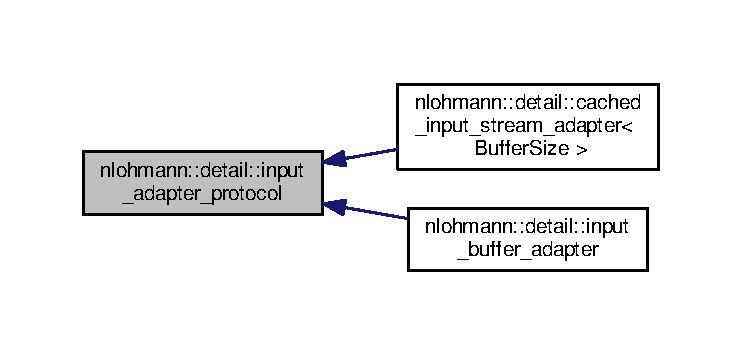
\includegraphics[width=350pt]{structnlohmann_1_1detail_1_1input__adapter__protocol__inherit__graph}
\end{center}
\end{figure}
\subsection*{Public Member Functions}
\begin{DoxyCompactItemize}
\item 
virtual int \hyperlink{structnlohmann_1_1detail_1_1input__adapter__protocol_af4e0baade0a6b45a73d4e136875e7544}{get\+\_\+character} ()=0
\item 
virtual \hyperlink{namespacenlohmann_1_1detail_a90aa5ef615aa8305e9ea20d8a947980fab45cffe084dd3d20d928bee85e7b0f21}{std\+::string} \hyperlink{structnlohmann_1_1detail_1_1input__adapter__protocol_a9ce6c8028229446d7014c0610fbd4599}{read} (std\+::size\+\_\+t offset, std\+::size\+\_\+t length)=0
\item 
virtual \hyperlink{structnlohmann_1_1detail_1_1input__adapter__protocol_a92dac74def4ac5adacd0684088bd4082}{$\sim$input\+\_\+adapter\+\_\+protocol} ()=default
\end{DoxyCompactItemize}


\subsection{Detailed Description}
abstract input adapter interface 

Definition at line 1294 of file json.\+hpp.



\subsection{Constructor \& Destructor Documentation}
\index{nlohmann\+::detail\+::input\+\_\+adapter\+\_\+protocol@{nlohmann\+::detail\+::input\+\_\+adapter\+\_\+protocol}!````~input\+\_\+adapter\+\_\+protocol@{$\sim$input\+\_\+adapter\+\_\+protocol}}
\index{````~input\+\_\+adapter\+\_\+protocol@{$\sim$input\+\_\+adapter\+\_\+protocol}!nlohmann\+::detail\+::input\+\_\+adapter\+\_\+protocol@{nlohmann\+::detail\+::input\+\_\+adapter\+\_\+protocol}}
\subsubsection[{\texorpdfstring{$\sim$input\+\_\+adapter\+\_\+protocol()=default}{~input_adapter_protocol()=default}}]{\setlength{\rightskip}{0pt plus 5cm}virtual nlohmann\+::detail\+::input\+\_\+adapter\+\_\+protocol\+::$\sim$input\+\_\+adapter\+\_\+protocol (
\begin{DoxyParamCaption}
{}
\end{DoxyParamCaption}
)\hspace{0.3cm}{\ttfamily [virtual]}, {\ttfamily [default]}}\hypertarget{structnlohmann_1_1detail_1_1input__adapter__protocol_a92dac74def4ac5adacd0684088bd4082}{}\label{structnlohmann_1_1detail_1_1input__adapter__protocol_a92dac74def4ac5adacd0684088bd4082}


\subsection{Member Function Documentation}
\index{nlohmann\+::detail\+::input\+\_\+adapter\+\_\+protocol@{nlohmann\+::detail\+::input\+\_\+adapter\+\_\+protocol}!get\+\_\+character@{get\+\_\+character}}
\index{get\+\_\+character@{get\+\_\+character}!nlohmann\+::detail\+::input\+\_\+adapter\+\_\+protocol@{nlohmann\+::detail\+::input\+\_\+adapter\+\_\+protocol}}
\subsubsection[{\texorpdfstring{get\+\_\+character()=0}{get_character()=0}}]{\setlength{\rightskip}{0pt plus 5cm}virtual int nlohmann\+::detail\+::input\+\_\+adapter\+\_\+protocol\+::get\+\_\+character (
\begin{DoxyParamCaption}
{}
\end{DoxyParamCaption}
)\hspace{0.3cm}{\ttfamily [pure virtual]}}\hypertarget{structnlohmann_1_1detail_1_1input__adapter__protocol_af4e0baade0a6b45a73d4e136875e7544}{}\label{structnlohmann_1_1detail_1_1input__adapter__protocol_af4e0baade0a6b45a73d4e136875e7544}


Implemented in \hyperlink{classnlohmann_1_1detail_1_1input__buffer__adapter_a3f03f910db299a9066923ddcccdb8a3c}{nlohmann\+::detail\+::input\+\_\+buffer\+\_\+adapter}, and \hyperlink{classnlohmann_1_1detail_1_1cached__input__stream__adapter_a4a6fc864751cf727b134f1c2bf31b523}{nlohmann\+::detail\+::cached\+\_\+input\+\_\+stream\+\_\+adapter$<$ Buffer\+Size $>$}.

\index{nlohmann\+::detail\+::input\+\_\+adapter\+\_\+protocol@{nlohmann\+::detail\+::input\+\_\+adapter\+\_\+protocol}!read@{read}}
\index{read@{read}!nlohmann\+::detail\+::input\+\_\+adapter\+\_\+protocol@{nlohmann\+::detail\+::input\+\_\+adapter\+\_\+protocol}}
\subsubsection[{\texorpdfstring{read(std\+::size\+\_\+t offset, std\+::size\+\_\+t length)=0}{read(std::size_t offset, std::size_t length)=0}}]{\setlength{\rightskip}{0pt plus 5cm}virtual {\bf std\+::string} nlohmann\+::detail\+::input\+\_\+adapter\+\_\+protocol\+::read (
\begin{DoxyParamCaption}
\item[{std\+::size\+\_\+t}]{offset, }
\item[{std\+::size\+\_\+t}]{length}
\end{DoxyParamCaption}
)\hspace{0.3cm}{\ttfamily [pure virtual]}}\hypertarget{structnlohmann_1_1detail_1_1input__adapter__protocol_a9ce6c8028229446d7014c0610fbd4599}{}\label{structnlohmann_1_1detail_1_1input__adapter__protocol_a9ce6c8028229446d7014c0610fbd4599}


Implemented in \hyperlink{classnlohmann_1_1detail_1_1input__buffer__adapter_af124e55c96814ae3a272dd5f0cb5351b}{nlohmann\+::detail\+::input\+\_\+buffer\+\_\+adapter}, and \hyperlink{classnlohmann_1_1detail_1_1cached__input__stream__adapter_ab9531a66a29685ec87646e99b516c263}{nlohmann\+::detail\+::cached\+\_\+input\+\_\+stream\+\_\+adapter$<$ Buffer\+Size $>$}.



The documentation for this struct was generated from the following file\+:\begin{DoxyCompactItemize}
\item 
include/\hyperlink{json_8hpp}{json.\+hpp}\end{DoxyCompactItemize}

\hypertarget{classnlohmann_1_1detail_1_1input__buffer__adapter}{}\section{nlohmann\+:\+:detail\+:\+:input\+\_\+buffer\+\_\+adapter Class Reference}
\label{classnlohmann_1_1detail_1_1input__buffer__adapter}\index{nlohmann\+::detail\+::input\+\_\+buffer\+\_\+adapter@{nlohmann\+::detail\+::input\+\_\+buffer\+\_\+adapter}}


input adapter for buffer input  




{\ttfamily \#include $<$json.\+hpp$>$}



Inheritance diagram for nlohmann\+:\+:detail\+:\+:input\+\_\+buffer\+\_\+adapter\+:\nopagebreak
\begin{figure}[H]
\begin{center}
\leavevmode
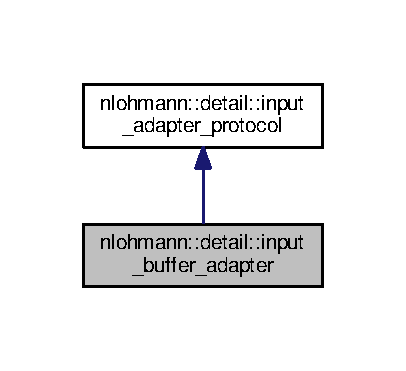
\includegraphics[width=195pt]{classnlohmann_1_1detail_1_1input__buffer__adapter__inherit__graph}
\end{center}
\end{figure}


Collaboration diagram for nlohmann\+:\+:detail\+:\+:input\+\_\+buffer\+\_\+adapter\+:\nopagebreak
\begin{figure}[H]
\begin{center}
\leavevmode
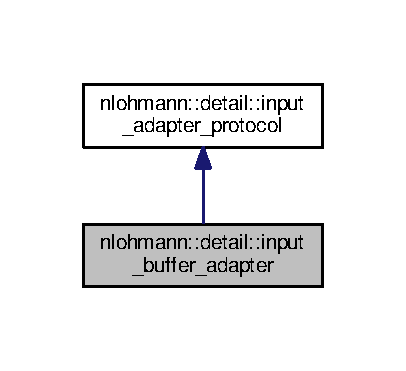
\includegraphics[width=195pt]{classnlohmann_1_1detail_1_1input__buffer__adapter__coll__graph}
\end{center}
\end{figure}
\subsection*{Public Member Functions}
\begin{DoxyCompactItemize}
\item 
\hyperlink{classnlohmann_1_1detail_1_1input__buffer__adapter_aee9d094d369bcd8f110eae4a175a8fa9}{input\+\_\+buffer\+\_\+adapter} (const char $\ast$b, const std\+::size\+\_\+t l)
\item 
\hyperlink{classnlohmann_1_1detail_1_1input__buffer__adapter_ada76d7b75c5d6b989af0e18687ef07b6}{input\+\_\+buffer\+\_\+adapter} (const \hyperlink{classnlohmann_1_1detail_1_1input__buffer__adapter}{input\+\_\+buffer\+\_\+adapter} \&)=delete
\item 
\hyperlink{classnlohmann_1_1detail_1_1input__buffer__adapter}{input\+\_\+buffer\+\_\+adapter} \& \hyperlink{classnlohmann_1_1detail_1_1input__buffer__adapter_a0871125057d993684ba8e45fb2b8a76b}{operator=} (\hyperlink{classnlohmann_1_1detail_1_1input__buffer__adapter}{input\+\_\+buffer\+\_\+adapter} \&)=delete
\item 
int \hyperlink{classnlohmann_1_1detail_1_1input__buffer__adapter_a3f03f910db299a9066923ddcccdb8a3c}{get\+\_\+character} () noexceptoverride
\item 
\hyperlink{namespacenlohmann_1_1detail_a90aa5ef615aa8305e9ea20d8a947980fab45cffe084dd3d20d928bee85e7b0f21}{std\+::string} \hyperlink{classnlohmann_1_1detail_1_1input__buffer__adapter_af124e55c96814ae3a272dd5f0cb5351b}{read} (std\+::size\+\_\+t offset, std\+::size\+\_\+t length) override
\end{DoxyCompactItemize}


\subsection{Detailed Description}
input adapter for buffer input 

Definition at line 1413 of file json.\+hpp.



\subsection{Constructor \& Destructor Documentation}
\index{nlohmann\+::detail\+::input\+\_\+buffer\+\_\+adapter@{nlohmann\+::detail\+::input\+\_\+buffer\+\_\+adapter}!input\+\_\+buffer\+\_\+adapter@{input\+\_\+buffer\+\_\+adapter}}
\index{input\+\_\+buffer\+\_\+adapter@{input\+\_\+buffer\+\_\+adapter}!nlohmann\+::detail\+::input\+\_\+buffer\+\_\+adapter@{nlohmann\+::detail\+::input\+\_\+buffer\+\_\+adapter}}
\subsubsection[{\texorpdfstring{input\+\_\+buffer\+\_\+adapter(const char $\ast$b, const std\+::size\+\_\+t l)}{input_buffer_adapter(const char *b, const std::size_t l)}}]{\setlength{\rightskip}{0pt plus 5cm}nlohmann\+::detail\+::input\+\_\+buffer\+\_\+adapter\+::input\+\_\+buffer\+\_\+adapter (
\begin{DoxyParamCaption}
\item[{const char $\ast$}]{b, }
\item[{const std\+::size\+\_\+t}]{l}
\end{DoxyParamCaption}
)\hspace{0.3cm}{\ttfamily [inline]}}\hypertarget{classnlohmann_1_1detail_1_1input__buffer__adapter_aee9d094d369bcd8f110eae4a175a8fa9}{}\label{classnlohmann_1_1detail_1_1input__buffer__adapter_aee9d094d369bcd8f110eae4a175a8fa9}


Definition at line 1416 of file json.\+hpp.

\index{nlohmann\+::detail\+::input\+\_\+buffer\+\_\+adapter@{nlohmann\+::detail\+::input\+\_\+buffer\+\_\+adapter}!input\+\_\+buffer\+\_\+adapter@{input\+\_\+buffer\+\_\+adapter}}
\index{input\+\_\+buffer\+\_\+adapter@{input\+\_\+buffer\+\_\+adapter}!nlohmann\+::detail\+::input\+\_\+buffer\+\_\+adapter@{nlohmann\+::detail\+::input\+\_\+buffer\+\_\+adapter}}
\subsubsection[{\texorpdfstring{input\+\_\+buffer\+\_\+adapter(const input\+\_\+buffer\+\_\+adapter \&)=delete}{input_buffer_adapter(const input_buffer_adapter &)=delete}}]{\setlength{\rightskip}{0pt plus 5cm}nlohmann\+::detail\+::input\+\_\+buffer\+\_\+adapter\+::input\+\_\+buffer\+\_\+adapter (
\begin{DoxyParamCaption}
\item[{const {\bf input\+\_\+buffer\+\_\+adapter} \&}]{}
\end{DoxyParamCaption}
)\hspace{0.3cm}{\ttfamily [delete]}}\hypertarget{classnlohmann_1_1detail_1_1input__buffer__adapter_ada76d7b75c5d6b989af0e18687ef07b6}{}\label{classnlohmann_1_1detail_1_1input__buffer__adapter_ada76d7b75c5d6b989af0e18687ef07b6}


\subsection{Member Function Documentation}
\index{nlohmann\+::detail\+::input\+\_\+buffer\+\_\+adapter@{nlohmann\+::detail\+::input\+\_\+buffer\+\_\+adapter}!get\+\_\+character@{get\+\_\+character}}
\index{get\+\_\+character@{get\+\_\+character}!nlohmann\+::detail\+::input\+\_\+buffer\+\_\+adapter@{nlohmann\+::detail\+::input\+\_\+buffer\+\_\+adapter}}
\subsubsection[{\texorpdfstring{get\+\_\+character() noexceptoverride}{get_character() noexceptoverride}}]{\setlength{\rightskip}{0pt plus 5cm}int nlohmann\+::detail\+::input\+\_\+buffer\+\_\+adapter\+::get\+\_\+character (
\begin{DoxyParamCaption}
{}
\end{DoxyParamCaption}
)\hspace{0.3cm}{\ttfamily [inline]}, {\ttfamily [override]}, {\ttfamily [virtual]}, {\ttfamily [noexcept]}}\hypertarget{classnlohmann_1_1detail_1_1input__buffer__adapter_a3f03f910db299a9066923ddcccdb8a3c}{}\label{classnlohmann_1_1detail_1_1input__buffer__adapter_a3f03f910db299a9066923ddcccdb8a3c}


Implements \hyperlink{structnlohmann_1_1detail_1_1input__adapter__protocol_af4e0baade0a6b45a73d4e136875e7544}{nlohmann\+::detail\+::input\+\_\+adapter\+\_\+protocol}.



Definition at line 1430 of file json.\+hpp.

\index{nlohmann\+::detail\+::input\+\_\+buffer\+\_\+adapter@{nlohmann\+::detail\+::input\+\_\+buffer\+\_\+adapter}!operator=@{operator=}}
\index{operator=@{operator=}!nlohmann\+::detail\+::input\+\_\+buffer\+\_\+adapter@{nlohmann\+::detail\+::input\+\_\+buffer\+\_\+adapter}}
\subsubsection[{\texorpdfstring{operator=(input\+\_\+buffer\+\_\+adapter \&)=delete}{operator=(input_buffer_adapter &)=delete}}]{\setlength{\rightskip}{0pt plus 5cm}{\bf input\+\_\+buffer\+\_\+adapter}\& nlohmann\+::detail\+::input\+\_\+buffer\+\_\+adapter\+::operator= (
\begin{DoxyParamCaption}
\item[{{\bf input\+\_\+buffer\+\_\+adapter} \&}]{}
\end{DoxyParamCaption}
)\hspace{0.3cm}{\ttfamily [delete]}}\hypertarget{classnlohmann_1_1detail_1_1input__buffer__adapter_a0871125057d993684ba8e45fb2b8a76b}{}\label{classnlohmann_1_1detail_1_1input__buffer__adapter_a0871125057d993684ba8e45fb2b8a76b}
\index{nlohmann\+::detail\+::input\+\_\+buffer\+\_\+adapter@{nlohmann\+::detail\+::input\+\_\+buffer\+\_\+adapter}!read@{read}}
\index{read@{read}!nlohmann\+::detail\+::input\+\_\+buffer\+\_\+adapter@{nlohmann\+::detail\+::input\+\_\+buffer\+\_\+adapter}}
\subsubsection[{\texorpdfstring{read(std\+::size\+\_\+t offset, std\+::size\+\_\+t length) override}{read(std::size_t offset, std::size_t length) override}}]{\setlength{\rightskip}{0pt plus 5cm}{\bf std\+::string} nlohmann\+::detail\+::input\+\_\+buffer\+\_\+adapter\+::read (
\begin{DoxyParamCaption}
\item[{std\+::size\+\_\+t}]{offset, }
\item[{std\+::size\+\_\+t}]{length}
\end{DoxyParamCaption}
)\hspace{0.3cm}{\ttfamily [inline]}, {\ttfamily [override]}, {\ttfamily [virtual]}}\hypertarget{classnlohmann_1_1detail_1_1input__buffer__adapter_af124e55c96814ae3a272dd5f0cb5351b}{}\label{classnlohmann_1_1detail_1_1input__buffer__adapter_af124e55c96814ae3a272dd5f0cb5351b}


Implements \hyperlink{structnlohmann_1_1detail_1_1input__adapter__protocol_a9ce6c8028229446d7014c0610fbd4599}{nlohmann\+::detail\+::input\+\_\+adapter\+\_\+protocol}.



Definition at line 1440 of file json.\+hpp.



The documentation for this class was generated from the following file\+:\begin{DoxyCompactItemize}
\item 
include/\hyperlink{json_8hpp}{json.\+hpp}\end{DoxyCompactItemize}

\hypertarget{structnlohmann_1_1detail_1_1internal__iterator}{}\section{nlohmann\+:\+:detail\+:\+:internal\+\_\+iterator$<$ Basic\+Json\+Type $>$ Struct Template Reference}
\label{structnlohmann_1_1detail_1_1internal__iterator}\index{nlohmann\+::detail\+::internal\+\_\+iterator$<$ Basic\+Json\+Type $>$@{nlohmann\+::detail\+::internal\+\_\+iterator$<$ Basic\+Json\+Type $>$}}


an iterator value  




{\ttfamily \#include $<$json.\+hpp$>$}



Collaboration diagram for nlohmann\+:\+:detail\+:\+:internal\+\_\+iterator$<$ Basic\+Json\+Type $>$\+:\nopagebreak
\begin{figure}[H]
\begin{center}
\leavevmode
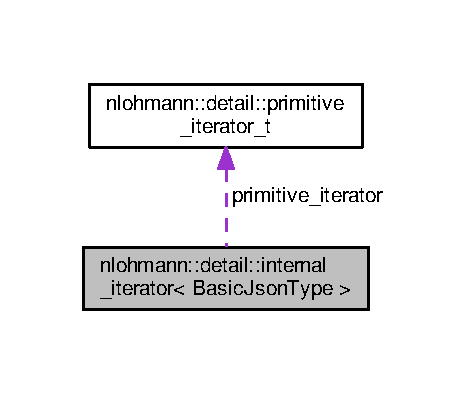
\includegraphics[width=225pt]{structnlohmann_1_1detail_1_1internal__iterator__coll__graph}
\end{center}
\end{figure}
\subsection*{Public Attributes}
\begin{DoxyCompactItemize}
\item 
Basic\+Json\+Type\+::object\+\_\+t\+::iterator \hyperlink{structnlohmann_1_1detail_1_1internal__iterator_a8cb0af3498061426c1d0a65ad6220408}{object\+\_\+iterator} \{\}
\begin{DoxyCompactList}\small\item\em iterator for J\+S\+ON objects \end{DoxyCompactList}\item 
Basic\+Json\+Type\+::array\+\_\+t\+::iterator \hyperlink{structnlohmann_1_1detail_1_1internal__iterator_a8294a6e6f01b58e1cce8fbae66a50b5d}{array\+\_\+iterator} \{\}
\begin{DoxyCompactList}\small\item\em iterator for J\+S\+ON arrays \end{DoxyCompactList}\item 
\hyperlink{classnlohmann_1_1detail_1_1primitive__iterator__t}{primitive\+\_\+iterator\+\_\+t} \hyperlink{structnlohmann_1_1detail_1_1internal__iterator_a2b3bb45f968210e42c282017eeeb63a8}{primitive\+\_\+iterator} \{\}
\begin{DoxyCompactList}\small\item\em generic iterator for all other types \end{DoxyCompactList}\end{DoxyCompactItemize}


\subsection{Detailed Description}
\subsubsection*{template$<$typename Basic\+Json\+Type$>$\\*
struct nlohmann\+::detail\+::internal\+\_\+iterator$<$ Basic\+Json\+Type $>$}

an iterator value 

\begin{DoxyNote}{Note}
This structure could easily be a union, but M\+S\+VC currently does not allow unions members with complex constructors, see \href{https://github.com/nlohmann/json/pull/105}{\tt https\+://github.\+com/nlohmann/json/pull/105}. 
\end{DoxyNote}


Definition at line 3524 of file json.\+hpp.



\subsection{Member Data Documentation}
\index{nlohmann\+::detail\+::internal\+\_\+iterator@{nlohmann\+::detail\+::internal\+\_\+iterator}!array\+\_\+iterator@{array\+\_\+iterator}}
\index{array\+\_\+iterator@{array\+\_\+iterator}!nlohmann\+::detail\+::internal\+\_\+iterator@{nlohmann\+::detail\+::internal\+\_\+iterator}}
\subsubsection[{\texorpdfstring{array\+\_\+iterator}{array_iterator}}]{\setlength{\rightskip}{0pt plus 5cm}template$<$typename Basic\+Json\+Type$>$ Basic\+Json\+Type\+::array\+\_\+t\+::iterator {\bf nlohmann\+::detail\+::internal\+\_\+iterator}$<$ Basic\+Json\+Type $>$\+::array\+\_\+iterator \{\}}\hypertarget{structnlohmann_1_1detail_1_1internal__iterator_a8294a6e6f01b58e1cce8fbae66a50b5d}{}\label{structnlohmann_1_1detail_1_1internal__iterator_a8294a6e6f01b58e1cce8fbae66a50b5d}


iterator for J\+S\+ON arrays 



Definition at line 3529 of file json.\+hpp.

\index{nlohmann\+::detail\+::internal\+\_\+iterator@{nlohmann\+::detail\+::internal\+\_\+iterator}!object\+\_\+iterator@{object\+\_\+iterator}}
\index{object\+\_\+iterator@{object\+\_\+iterator}!nlohmann\+::detail\+::internal\+\_\+iterator@{nlohmann\+::detail\+::internal\+\_\+iterator}}
\subsubsection[{\texorpdfstring{object\+\_\+iterator}{object_iterator}}]{\setlength{\rightskip}{0pt plus 5cm}template$<$typename Basic\+Json\+Type$>$ Basic\+Json\+Type\+::object\+\_\+t\+::iterator {\bf nlohmann\+::detail\+::internal\+\_\+iterator}$<$ Basic\+Json\+Type $>$\+::object\+\_\+iterator \{\}}\hypertarget{structnlohmann_1_1detail_1_1internal__iterator_a8cb0af3498061426c1d0a65ad6220408}{}\label{structnlohmann_1_1detail_1_1internal__iterator_a8cb0af3498061426c1d0a65ad6220408}


iterator for J\+S\+ON objects 



Definition at line 3527 of file json.\+hpp.

\index{nlohmann\+::detail\+::internal\+\_\+iterator@{nlohmann\+::detail\+::internal\+\_\+iterator}!primitive\+\_\+iterator@{primitive\+\_\+iterator}}
\index{primitive\+\_\+iterator@{primitive\+\_\+iterator}!nlohmann\+::detail\+::internal\+\_\+iterator@{nlohmann\+::detail\+::internal\+\_\+iterator}}
\subsubsection[{\texorpdfstring{primitive\+\_\+iterator}{primitive_iterator}}]{\setlength{\rightskip}{0pt plus 5cm}template$<$typename Basic\+Json\+Type$>$ {\bf primitive\+\_\+iterator\+\_\+t} {\bf nlohmann\+::detail\+::internal\+\_\+iterator}$<$ Basic\+Json\+Type $>$\+::primitive\+\_\+iterator \{\}}\hypertarget{structnlohmann_1_1detail_1_1internal__iterator_a2b3bb45f968210e42c282017eeeb63a8}{}\label{structnlohmann_1_1detail_1_1internal__iterator_a2b3bb45f968210e42c282017eeeb63a8}


generic iterator for all other types 



Definition at line 3531 of file json.\+hpp.



The documentation for this struct was generated from the following file\+:\begin{DoxyCompactItemize}
\item 
include/\hyperlink{json_8hpp}{json.\+hpp}\end{DoxyCompactItemize}

\hypertarget{class_internal_register}{}\section{Internal\+Register Class Reference}
\label{class_internal_register}\index{Internal\+Register@{Internal\+Register}}


{\ttfamily \#include $<$I2\+C\+Register.\+hpp$>$}



Inheritance diagram for Internal\+Register\+:\nopagebreak
\begin{figure}[H]
\begin{center}
\leavevmode
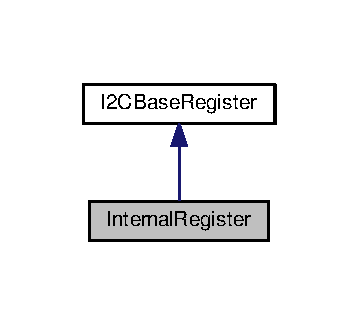
\includegraphics[width=172pt]{class_internal_register__inherit__graph}
\end{center}
\end{figure}


Collaboration diagram for Internal\+Register\+:\nopagebreak
\begin{figure}[H]
\begin{center}
\leavevmode
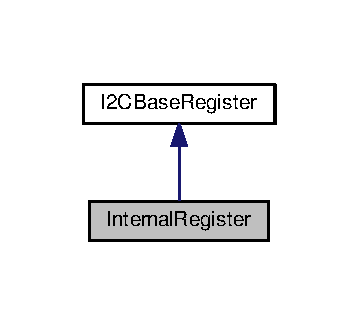
\includegraphics[width=172pt]{class_internal_register__coll__graph}
\end{center}
\end{figure}
\subsection*{Public Member Functions}
\begin{DoxyCompactItemize}
\item 
\hyperlink{class_internal_register_a09cee9a73ce992860d9ea3353c9e9e9c}{Internal\+Register} (uint32\+\_\+t r, std\+::string rw, std\+::function$<$ \hyperlink{units__define_8hpp_a95d46867fa79633565c288a0b4bd5408}{units\+\_\+variant}(double value)$>$ read\+\_\+func)
\begin{DoxyCompactList}\small\item\em Class constructor. \end{DoxyCompactList}\item 
\hyperlink{class_internal_register_adee7135b7fb2f55576b07c6440c1a2d9}{$\sim$\+Internal\+Register} (void)
\begin{DoxyCompactList}\small\item\em Class destructor. \end{DoxyCompactList}\item 
\hyperlink{units__define_8hpp_a95d46867fa79633565c288a0b4bd5408}{units\+\_\+variant} \hyperlink{class_internal_register_a7675a310cdb4866c256fef77d388b424}{read} (\hyperlink{class_i2_c__base}{I2\+C\+\_\+base} $\ast$i2c\+\_\+ptr, uint32\+\_\+t address)
\begin{DoxyCompactList}\small\item\em Read data from register. \end{DoxyCompactList}\item 
void \hyperlink{class_internal_register_a8c1844d644fc81a118a6094f3a88feb8}{write} (\hyperlink{class_i2_c__base}{I2\+C\+\_\+base} $\ast$i2c\+\_\+ptr, uint32\+\_\+t address, \hyperlink{units__define_8hpp_a95d46867fa79633565c288a0b4bd5408}{units\+\_\+variant} value)
\begin{DoxyCompactList}\small\item\em V\+A\+L\+U\+ES C\+A\+N\+N\+OT BE W\+R\+I\+T\+T\+EN TO. \end{DoxyCompactList}\end{DoxyCompactItemize}
\subsection*{Additional Inherited Members}


\subsection{Detailed Description}


Definition at line 89 of file I2\+C\+Register.\+hpp.



\subsection{Constructor \& Destructor Documentation}
\index{Internal\+Register@{Internal\+Register}!Internal\+Register@{Internal\+Register}}
\index{Internal\+Register@{Internal\+Register}!Internal\+Register@{Internal\+Register}}
\subsubsection[{\texorpdfstring{Internal\+Register(uint32\+\_\+t r, std\+::string rw, std\+::function$<$ units\+\_\+variant(double value)$>$ read\+\_\+func)}{InternalRegister(uint32_t r, std::string rw, std::function< units_variant(double value)> read_func)}}]{\setlength{\rightskip}{0pt plus 5cm}Internal\+Register\+::\+Internal\+Register (
\begin{DoxyParamCaption}
\item[{uint32\+\_\+t}]{r, }
\item[{std\+::string}]{rw, }
\item[{std\+::function$<$ {\bf units\+\_\+variant}(double value)$>$}]{read\+\_\+func}
\end{DoxyParamCaption}
)}\hypertarget{class_internal_register_a09cee9a73ce992860d9ea3353c9e9e9c}{}\label{class_internal_register_a09cee9a73ce992860d9ea3353c9e9e9c}


Class constructor. 


\begin{DoxyParams}{Parameters}
{\em read\+\_\+func} & -\/ Lambda function to convert hexadecimal value into correct units type. \\
\hline
{\em write\+\_\+func} & -\/ Lambda function to convert units type into uint8\+\_\+t to be written. \\
\hline
\end{DoxyParams}


Definition at line 70 of file I2\+C\+Register.\+cpp.

\index{Internal\+Register@{Internal\+Register}!````~Internal\+Register@{$\sim$\+Internal\+Register}}
\index{````~Internal\+Register@{$\sim$\+Internal\+Register}!Internal\+Register@{Internal\+Register}}
\subsubsection[{\texorpdfstring{$\sim$\+Internal\+Register(void)}{~InternalRegister(void)}}]{\setlength{\rightskip}{0pt plus 5cm}Internal\+Register\+::$\sim$\+Internal\+Register (
\begin{DoxyParamCaption}
\item[{void}]{}
\end{DoxyParamCaption}
)}\hypertarget{class_internal_register_adee7135b7fb2f55576b07c6440c1a2d9}{}\label{class_internal_register_adee7135b7fb2f55576b07c6440c1a2d9}


Class destructor. 



Definition at line 84 of file I2\+C\+Register.\+cpp.



\subsection{Member Function Documentation}
\index{Internal\+Register@{Internal\+Register}!read@{read}}
\index{read@{read}!Internal\+Register@{Internal\+Register}}
\subsubsection[{\texorpdfstring{read(\+I2\+C\+\_\+base $\ast$i2c\+\_\+ptr, uint32\+\_\+t address)}{read(I2C_base *i2c_ptr, uint32_t address)}}]{\setlength{\rightskip}{0pt plus 5cm}{\bf units\+\_\+variant} Internal\+Register\+::read (
\begin{DoxyParamCaption}
\item[{{\bf I2\+C\+\_\+base} $\ast$}]{i2c\+\_\+ptr, }
\item[{uint32\+\_\+t}]{address}
\end{DoxyParamCaption}
)\hspace{0.3cm}{\ttfamily [virtual]}}\hypertarget{class_internal_register_a7675a310cdb4866c256fef77d388b424}{}\label{class_internal_register_a7675a310cdb4866c256fef77d388b424}


Read data from register. 


\begin{DoxyParams}{Parameters}
{\em i2c\+\_\+ptr} & -\/ Pointer to \hyperlink{class_i2_c__base}{I2\+C\+\_\+base} class used for transport. \\
\hline
\end{DoxyParams}
\begin{DoxyReturn}{Returns}
units\+\_\+variant containing quantity of correct type. 
\end{DoxyReturn}


Implements \hyperlink{class_i2_c_base_register_a947d834a745d3036c4cd8a2d5e19cd0d}{I2\+C\+Base\+Register}.



Definition at line 91 of file I2\+C\+Register.\+cpp.

\index{Internal\+Register@{Internal\+Register}!write@{write}}
\index{write@{write}!Internal\+Register@{Internal\+Register}}
\subsubsection[{\texorpdfstring{write(\+I2\+C\+\_\+base $\ast$i2c\+\_\+ptr, uint32\+\_\+t address, units\+\_\+variant value)}{write(I2C_base *i2c_ptr, uint32_t address, units_variant value)}}]{\setlength{\rightskip}{0pt plus 5cm}void Internal\+Register\+::write (
\begin{DoxyParamCaption}
\item[{{\bf I2\+C\+\_\+base} $\ast$}]{i2c\+\_\+ptr, }
\item[{uint32\+\_\+t}]{address, }
\item[{{\bf units\+\_\+variant}}]{value}
\end{DoxyParamCaption}
)\hspace{0.3cm}{\ttfamily [virtual]}}\hypertarget{class_internal_register_a8c1844d644fc81a118a6094f3a88feb8}{}\label{class_internal_register_a8c1844d644fc81a118a6094f3a88feb8}


V\+A\+L\+U\+ES C\+A\+N\+N\+OT BE W\+R\+I\+T\+T\+EN TO. 


\begin{DoxyParams}{Parameters}
{\em i2c\+\_\+ptr} & -\/ Pointer to \hyperlink{class_i2_c__base}{I2\+C\+\_\+base} class used for transport. \\
\hline
{\em value} & -\/ Data to be written. Must be of correct type. \\
\hline
\end{DoxyParams}


Implements \hyperlink{class_i2_c_base_register_ad3f9f1404fe6af3e10e8f204b16d2066}{I2\+C\+Base\+Register}.



Definition at line 107 of file I2\+C\+Register.\+cpp.



The documentation for this class was generated from the following files\+:\begin{DoxyCompactItemize}
\item 
include/\hyperlink{_i2_c_register_8hpp}{I2\+C\+Register.\+hpp}\item 
src/\hyperlink{_i2_c_register_8cpp}{I2\+C\+Register.\+cpp}\end{DoxyCompactItemize}

\hypertarget{classnlohmann_1_1detail_1_1invalid__iterator}{}\section{nlohmann\+:\+:detail\+:\+:invalid\+\_\+iterator Class Reference}
\label{classnlohmann_1_1detail_1_1invalid__iterator}\index{nlohmann\+::detail\+::invalid\+\_\+iterator@{nlohmann\+::detail\+::invalid\+\_\+iterator}}


exception indicating errors with iterators  




{\ttfamily \#include $<$json.\+hpp$>$}



Inheritance diagram for nlohmann\+:\+:detail\+:\+:invalid\+\_\+iterator\+:\nopagebreak
\begin{figure}[H]
\begin{center}
\leavevmode
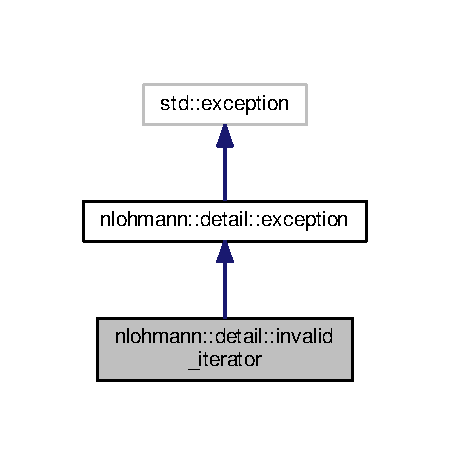
\includegraphics[width=216pt]{classnlohmann_1_1detail_1_1invalid__iterator__inherit__graph}
\end{center}
\end{figure}


Collaboration diagram for nlohmann\+:\+:detail\+:\+:invalid\+\_\+iterator\+:\nopagebreak
\begin{figure}[H]
\begin{center}
\leavevmode
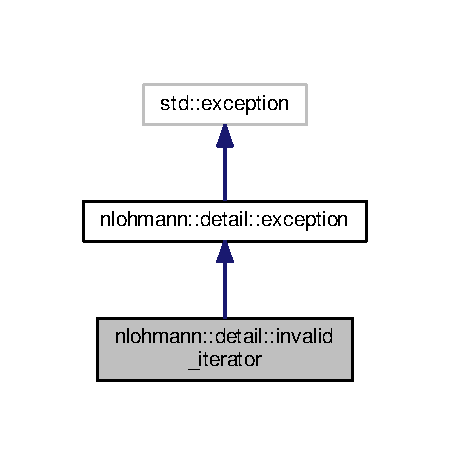
\includegraphics[width=216pt]{classnlohmann_1_1detail_1_1invalid__iterator__coll__graph}
\end{center}
\end{figure}
\subsection*{Static Public Member Functions}
\begin{DoxyCompactItemize}
\item 
static \hyperlink{classnlohmann_1_1detail_1_1invalid__iterator}{invalid\+\_\+iterator} \hyperlink{classnlohmann_1_1detail_1_1invalid__iterator_a48d724eccc74b550d695fc7575d9ce30}{create} (int \hyperlink{classnlohmann_1_1detail_1_1exception_a0d4589a3fb54e81646d986c05efa3b9a}{id}, const \hyperlink{namespacenlohmann_1_1detail_a90aa5ef615aa8305e9ea20d8a947980fab45cffe084dd3d20d928bee85e7b0f21}{std\+::string} \&what\+\_\+arg)
\end{DoxyCompactItemize}
\subsection*{Additional Inherited Members}


\subsection{Detailed Description}
exception indicating errors with iterators 

Exceptions have ids 2xx.

\tabulinesep=1mm
\begin{longtabu} spread 0pt [c]{*3{|X[-1]}|}
\hline
\rowcolor{\tableheadbgcolor}{\bf name / id }&{\bf example massage }&{\bf description  }\\\cline{1-3}
\endfirsthead
\hline
\endfoot
\hline
\rowcolor{\tableheadbgcolor}{\bf name / id }&{\bf example massage }&{\bf description  }\\\cline{1-3}
\endhead
json.\+exception.\+invalid\+\_\+iterator.\+201 &iterators are not compatible &The iterators passed to constructor basic\+\_\+json(\+Input\+I\+T first, Input\+I\+T last) are not compatible, meaning they do not belong to the same container. Therefore, the range ({\itshape first}, {\itshape last}) is invalid. \\\cline{1-3}
json.\+exception.\+invalid\+\_\+iterator.\+202 &iterator does not fit current value &In an erase or insert function, the passed iterator {\itshape pos} does not belong to the J\+S\+ON value for which the function was called. It hence does not define a valid position for the deletion/insertion. \\\cline{1-3}
json.\+exception.\+invalid\+\_\+iterator.\+203 &iterators do not fit current value &Either iterator passed to function erase(\+Iterator\+Type first, Iterator\+Type last) does not belong to the J\+S\+ON value from which values shall be erased. It hence does not define a valid range to delete values from. \\\cline{1-3}
json.\+exception.\+invalid\+\_\+iterator.\+204 &iterators out of range &When an iterator range for a primitive type (number, boolean, or string) is passed to a constructor or an erase function, this range has to be exactly (begin(), end()), because this is the only way the single stored value is expressed. All other ranges are invalid. \\\cline{1-3}
json.\+exception.\+invalid\+\_\+iterator.\+205 &iterator out of range &When an iterator for a primitive type (number, boolean, or string) is passed to an erase function, the iterator has to be the begin() iterator, because it is the only way to address the stored value. All other iterators are invalid. \\\cline{1-3}
json.\+exception.\+invalid\+\_\+iterator.\+206 &cannot construct with iterators from null &The iterators passed to constructor basic\+\_\+json(\+Input\+I\+T first, Input\+I\+T last) belong to a J\+S\+ON null value and hence to not define a valid range. \\\cline{1-3}
json.\+exception.\+invalid\+\_\+iterator.\+207 &cannot use key() for non-\/object iterators &The key() member function can only be used on iterators belonging to a J\+S\+ON object, because other types do not have a concept of a key. \\\cline{1-3}
json.\+exception.\+invalid\+\_\+iterator.\+208 &cannot use operator\mbox{[}\mbox{]} for object iterators &The operator\mbox{[}\mbox{]} to specify a concrete offset cannot be used on iterators belonging to a J\+S\+ON object, because J\+S\+ON objects are unordered. \\\cline{1-3}
json.\+exception.\+invalid\+\_\+iterator.\+209 &cannot use offsets with object iterators &The offset operators (+, -\/, +=, -\/=) cannot be used on iterators belonging to a J\+S\+ON object, because J\+S\+ON objects are unordered. \\\cline{1-3}
json.\+exception.\+invalid\+\_\+iterator.\+210 &iterators do not fit &The iterator range passed to the insert function are not compatible, meaning they do not belong to the same container. Therefore, the range ({\itshape first}, {\itshape last}) is invalid. \\\cline{1-3}
json.\+exception.\+invalid\+\_\+iterator.\+211 &passed iterators may not belong to container &The iterator range passed to the insert function must not be a subrange of the container to insert to. \\\cline{1-3}
json.\+exception.\+invalid\+\_\+iterator.\+212 &cannot compare iterators of different containers &When two iterators are compared, they must belong to the same container. \\\cline{1-3}
json.\+exception.\+invalid\+\_\+iterator.\+213 &cannot compare order of object iterators &The order of object iterators cannot be compared, because J\+S\+ON objects are unordered. \\\cline{1-3}
json.\+exception.\+invalid\+\_\+iterator.\+214 &cannot get value &Cannot get value for iterator\+: Either the iterator belongs to a null value or it is an iterator to a primitive type (number, boolean, or string), but the iterator is different to begin(). \\\cline{1-3}
\end{longtabu}
\begin{DoxySince}{Since}
version 3.\+0.\+0 
\end{DoxySince}


Definition at line 294 of file json.\+hpp.



\subsection{Member Function Documentation}
\index{nlohmann\+::detail\+::invalid\+\_\+iterator@{nlohmann\+::detail\+::invalid\+\_\+iterator}!create@{create}}
\index{create@{create}!nlohmann\+::detail\+::invalid\+\_\+iterator@{nlohmann\+::detail\+::invalid\+\_\+iterator}}
\subsubsection[{\texorpdfstring{create(int id, const std\+::string \&what\+\_\+arg)}{create(int id, const std::string &what_arg)}}]{\setlength{\rightskip}{0pt plus 5cm}static {\bf invalid\+\_\+iterator} nlohmann\+::detail\+::invalid\+\_\+iterator\+::create (
\begin{DoxyParamCaption}
\item[{int}]{id, }
\item[{const {\bf std\+::string} \&}]{what\+\_\+arg}
\end{DoxyParamCaption}
)\hspace{0.3cm}{\ttfamily [inline]}, {\ttfamily [static]}}\hypertarget{classnlohmann_1_1detail_1_1invalid__iterator_a48d724eccc74b550d695fc7575d9ce30}{}\label{classnlohmann_1_1detail_1_1invalid__iterator_a48d724eccc74b550d695fc7575d9ce30}


Definition at line 297 of file json.\+hpp.



The documentation for this class was generated from the following file\+:\begin{DoxyCompactItemize}
\item 
include/\hyperlink{json_8hpp}{json.\+hpp}\end{DoxyCompactItemize}

\hypertarget{structnlohmann_1_1detail_1_1is__basic__json}{}\section{nlohmann\+:\+:detail\+:\+:is\+\_\+basic\+\_\+json$<$ typename $>$ Struct Template Reference}
\label{structnlohmann_1_1detail_1_1is__basic__json}\index{nlohmann\+::detail\+::is\+\_\+basic\+\_\+json$<$ typename $>$@{nlohmann\+::detail\+::is\+\_\+basic\+\_\+json$<$ typename $>$}}


{\ttfamily \#include $<$json.\+hpp$>$}



Inheritance diagram for nlohmann\+:\+:detail\+:\+:is\+\_\+basic\+\_\+json$<$ typename $>$\+:\nopagebreak
\begin{figure}[H]
\begin{center}
\leavevmode
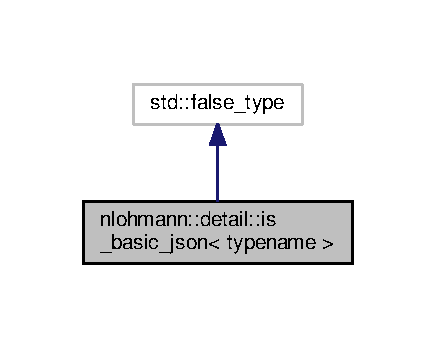
\includegraphics[width=209pt]{structnlohmann_1_1detail_1_1is__basic__json__inherit__graph}
\end{center}
\end{figure}


Collaboration diagram for nlohmann\+:\+:detail\+:\+:is\+\_\+basic\+\_\+json$<$ typename $>$\+:\nopagebreak
\begin{figure}[H]
\begin{center}
\leavevmode
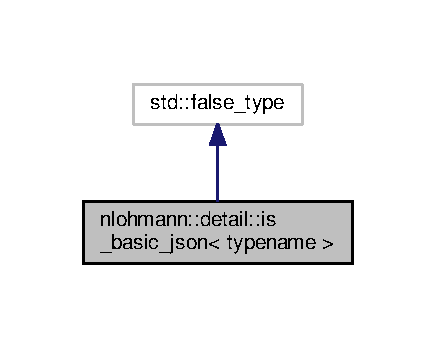
\includegraphics[width=209pt]{structnlohmann_1_1detail_1_1is__basic__json__coll__graph}
\end{center}
\end{figure}


\subsection{Detailed Description}
\subsubsection*{template$<$typename$>$\\*
struct nlohmann\+::detail\+::is\+\_\+basic\+\_\+json$<$ typename $>$}



Definition at line 480 of file json.\+hpp.



The documentation for this struct was generated from the following file\+:\begin{DoxyCompactItemize}
\item 
include/\hyperlink{json_8hpp}{json.\+hpp}\end{DoxyCompactItemize}

\hypertarget{structnlohmann_1_1detail_1_1is__basic__json_3_01_n_l_o_h_m_a_n_n___b_a_s_i_c___j_s_o_n___t_p_l_01_4}{}\section{nlohmann\+:\+:detail\+:\+:is\+\_\+basic\+\_\+json$<$ N\+L\+O\+H\+M\+A\+N\+N\+\_\+\+B\+A\+S\+I\+C\+\_\+\+J\+S\+O\+N\+\_\+\+T\+PL $>$ Struct Reference}
\label{structnlohmann_1_1detail_1_1is__basic__json_3_01_n_l_o_h_m_a_n_n___b_a_s_i_c___j_s_o_n___t_p_l_01_4}\index{nlohmann\+::detail\+::is\+\_\+basic\+\_\+json$<$ N\+L\+O\+H\+M\+A\+N\+N\+\_\+\+B\+A\+S\+I\+C\+\_\+\+J\+S\+O\+N\+\_\+\+T\+P\+L $>$@{nlohmann\+::detail\+::is\+\_\+basic\+\_\+json$<$ N\+L\+O\+H\+M\+A\+N\+N\+\_\+\+B\+A\+S\+I\+C\+\_\+\+J\+S\+O\+N\+\_\+\+T\+P\+L $>$}}


{\ttfamily \#include $<$json.\+hpp$>$}



Inheritance diagram for nlohmann\+:\+:detail\+:\+:is\+\_\+basic\+\_\+json$<$ N\+L\+O\+H\+M\+A\+N\+N\+\_\+\+B\+A\+S\+I\+C\+\_\+\+J\+S\+O\+N\+\_\+\+T\+PL $>$\+:\nopagebreak
\begin{figure}[H]
\begin{center}
\leavevmode
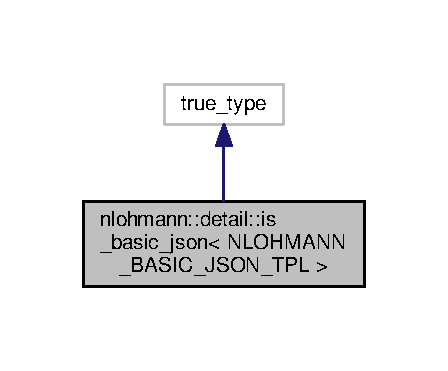
\includegraphics[width=215pt]{structnlohmann_1_1detail_1_1is__basic__json_3_01_n_l_o_h_m_a_n_n___b_a_s_i_c___j_s_o_n___t_p_l_01_4__inherit__graph}
\end{center}
\end{figure}


Collaboration diagram for nlohmann\+:\+:detail\+:\+:is\+\_\+basic\+\_\+json$<$ N\+L\+O\+H\+M\+A\+N\+N\+\_\+\+B\+A\+S\+I\+C\+\_\+\+J\+S\+O\+N\+\_\+\+T\+PL $>$\+:\nopagebreak
\begin{figure}[H]
\begin{center}
\leavevmode
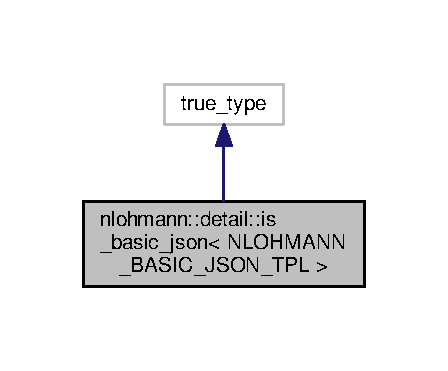
\includegraphics[width=215pt]{structnlohmann_1_1detail_1_1is__basic__json_3_01_n_l_o_h_m_a_n_n___b_a_s_i_c___j_s_o_n___t_p_l_01_4__coll__graph}
\end{center}
\end{figure}


\subsection{Detailed Description}


Definition at line 483 of file json.\+hpp.



The documentation for this struct was generated from the following file\+:\begin{DoxyCompactItemize}
\item 
include/\hyperlink{json_8hpp}{json.\+hpp}\end{DoxyCompactItemize}

\hypertarget{structnlohmann_1_1detail_1_1is__basic__json__nested__type}{}\section{nlohmann\+:\+:detail\+:\+:is\+\_\+basic\+\_\+json\+\_\+nested\+\_\+type$<$ Basic\+Json\+Type, T $>$ Struct Template Reference}
\label{structnlohmann_1_1detail_1_1is__basic__json__nested__type}\index{nlohmann\+::detail\+::is\+\_\+basic\+\_\+json\+\_\+nested\+\_\+type$<$ Basic\+Json\+Type, T $>$@{nlohmann\+::detail\+::is\+\_\+basic\+\_\+json\+\_\+nested\+\_\+type$<$ Basic\+Json\+Type, T $>$}}


{\ttfamily \#include $<$json.\+hpp$>$}

\subsection*{Static Public Attributes}
\begin{DoxyCompactItemize}
\item 
static auto constexpr \hyperlink{structnlohmann_1_1detail_1_1is__basic__json__nested__type_aee5fee744e5298a78d557f2ee5f090db}{value}
\end{DoxyCompactItemize}


\subsection{Detailed Description}
\subsubsection*{template$<$typename Basic\+Json\+Type, typename T$>$\\*
struct nlohmann\+::detail\+::is\+\_\+basic\+\_\+json\+\_\+nested\+\_\+type$<$ Basic\+Json\+Type, T $>$}



Definition at line 759 of file json.\+hpp.



\subsection{Member Data Documentation}
\index{nlohmann\+::detail\+::is\+\_\+basic\+\_\+json\+\_\+nested\+\_\+type@{nlohmann\+::detail\+::is\+\_\+basic\+\_\+json\+\_\+nested\+\_\+type}!value@{value}}
\index{value@{value}!nlohmann\+::detail\+::is\+\_\+basic\+\_\+json\+\_\+nested\+\_\+type@{nlohmann\+::detail\+::is\+\_\+basic\+\_\+json\+\_\+nested\+\_\+type}}
\subsubsection[{\texorpdfstring{value}{value}}]{\setlength{\rightskip}{0pt plus 5cm}template$<$typename Basic\+Json\+Type , typename T $>$ auto constexpr {\bf nlohmann\+::detail\+::is\+\_\+basic\+\_\+json\+\_\+nested\+\_\+type}$<$ Basic\+Json\+Type, T $>$\+::value\hspace{0.3cm}{\ttfamily [static]}}\hypertarget{structnlohmann_1_1detail_1_1is__basic__json__nested__type_aee5fee744e5298a78d557f2ee5f090db}{}\label{structnlohmann_1_1detail_1_1is__basic__json__nested__type_aee5fee744e5298a78d557f2ee5f090db}
{\bfseries Initial value\+:}
\begin{DoxyCode}
= std::is\_same<T, typename BasicJsonType::iterator>::value or
                                  std::is\_same<T, typename BasicJsonType::const\_iterator>::value or
                                  std::is\_same<T, typename BasicJsonType::reverse\_iterator>::value or
                                  std::is\_same<T, typename BasicJsonType::const\_reverse\_iterator>::value
\end{DoxyCode}


Definition at line 761 of file json.\+hpp.



The documentation for this struct was generated from the following file\+:\begin{DoxyCompactItemize}
\item 
include/\hyperlink{json_8hpp}{json.\+hpp}\end{DoxyCompactItemize}

\hypertarget{structnlohmann_1_1detail_1_1is__compatible__array__type}{}\section{nlohmann\+:\+:detail\+:\+:is\+\_\+compatible\+\_\+array\+\_\+type$<$ Basic\+Json\+Type, Compatible\+Array\+Type $>$ Struct Template Reference}
\label{structnlohmann_1_1detail_1_1is__compatible__array__type}\index{nlohmann\+::detail\+::is\+\_\+compatible\+\_\+array\+\_\+type$<$ Basic\+Json\+Type, Compatible\+Array\+Type $>$@{nlohmann\+::detail\+::is\+\_\+compatible\+\_\+array\+\_\+type$<$ Basic\+Json\+Type, Compatible\+Array\+Type $>$}}


{\ttfamily \#include $<$json.\+hpp$>$}

\subsection*{Static Public Attributes}
\begin{DoxyCompactItemize}
\item 
static auto constexpr \hyperlink{structnlohmann_1_1detail_1_1is__compatible__array__type_a01bc2274c22746bbb2cefd2acee8b572}{value}
\end{DoxyCompactItemize}


\subsection{Detailed Description}
\subsubsection*{template$<$class Basic\+Json\+Type, class Compatible\+Array\+Type$>$\\*
struct nlohmann\+::detail\+::is\+\_\+compatible\+\_\+array\+\_\+type$<$ Basic\+Json\+Type, Compatible\+Array\+Type $>$}



Definition at line 768 of file json.\+hpp.



\subsection{Member Data Documentation}
\index{nlohmann\+::detail\+::is\+\_\+compatible\+\_\+array\+\_\+type@{nlohmann\+::detail\+::is\+\_\+compatible\+\_\+array\+\_\+type}!value@{value}}
\index{value@{value}!nlohmann\+::detail\+::is\+\_\+compatible\+\_\+array\+\_\+type@{nlohmann\+::detail\+::is\+\_\+compatible\+\_\+array\+\_\+type}}
\subsubsection[{\texorpdfstring{value}{value}}]{\setlength{\rightskip}{0pt plus 5cm}template$<$class Basic\+Json\+Type , class Compatible\+Array\+Type $>$ auto constexpr {\bf nlohmann\+::detail\+::is\+\_\+compatible\+\_\+array\+\_\+type}$<$ Basic\+Json\+Type, Compatible\+Array\+Type $>$\+::value\hspace{0.3cm}{\ttfamily [static]}}\hypertarget{structnlohmann_1_1detail_1_1is__compatible__array__type_a01bc2274c22746bbb2cefd2acee8b572}{}\label{structnlohmann_1_1detail_1_1is__compatible__array__type_a01bc2274c22746bbb2cefd2acee8b572}
{\bfseries Initial value\+:}
\begin{DoxyCode}
=
        conjunction<negation<std::is\_same<void, CompatibleArrayType>>,
        negation<is\_compatible\_object\_type<
        BasicJsonType, CompatibleArrayType>>,
        negation<std::is\_constructible<\textcolor{keyword}{typename} BasicJsonType::string\_t,
        CompatibleArrayType>>,
        negation<is\_basic\_json\_nested\_type<BasicJsonType, CompatibleArrayType>>,
        has\_value\_type<CompatibleArrayType>,
        has\_iterator<CompatibleArrayType>>\hyperlink{structnlohmann_1_1detail_1_1is__compatible__array__type_a01bc2274c22746bbb2cefd2acee8b572}{::value}
\end{DoxyCode}


Definition at line 770 of file json.\+hpp.



The documentation for this struct was generated from the following file\+:\begin{DoxyCompactItemize}
\item 
include/\hyperlink{json_8hpp}{json.\+hpp}\end{DoxyCompactItemize}

\hypertarget{structnlohmann_1_1detail_1_1is__compatible__integer__type}{}\section{nlohmann\+:\+:detail\+:\+:is\+\_\+compatible\+\_\+integer\+\_\+type$<$ Real\+Integer\+Type, Compatible\+Number\+Integer\+Type $>$ Struct Template Reference}
\label{structnlohmann_1_1detail_1_1is__compatible__integer__type}\index{nlohmann\+::detail\+::is\+\_\+compatible\+\_\+integer\+\_\+type$<$ Real\+Integer\+Type, Compatible\+Number\+Integer\+Type $>$@{nlohmann\+::detail\+::is\+\_\+compatible\+\_\+integer\+\_\+type$<$ Real\+Integer\+Type, Compatible\+Number\+Integer\+Type $>$}}


{\ttfamily \#include $<$json.\+hpp$>$}

\subsection*{Static Public Attributes}
\begin{DoxyCompactItemize}
\item 
static constexpr auto \hyperlink{structnlohmann_1_1detail_1_1is__compatible__integer__type_ac5e5bd39773676564c73d3dd2a9c6e0a}{value}
\end{DoxyCompactItemize}


\subsection{Detailed Description}
\subsubsection*{template$<$typename Real\+Integer\+Type, typename Compatible\+Number\+Integer\+Type$>$\\*
struct nlohmann\+::detail\+::is\+\_\+compatible\+\_\+integer\+\_\+type$<$ Real\+Integer\+Type, Compatible\+Number\+Integer\+Type $>$}



Definition at line 798 of file json.\+hpp.



\subsection{Member Data Documentation}
\index{nlohmann\+::detail\+::is\+\_\+compatible\+\_\+integer\+\_\+type@{nlohmann\+::detail\+::is\+\_\+compatible\+\_\+integer\+\_\+type}!value@{value}}
\index{value@{value}!nlohmann\+::detail\+::is\+\_\+compatible\+\_\+integer\+\_\+type@{nlohmann\+::detail\+::is\+\_\+compatible\+\_\+integer\+\_\+type}}
\subsubsection[{\texorpdfstring{value}{value}}]{\setlength{\rightskip}{0pt plus 5cm}template$<$typename Real\+Integer\+Type , typename Compatible\+Number\+Integer\+Type $>$ constexpr auto {\bf nlohmann\+::detail\+::is\+\_\+compatible\+\_\+integer\+\_\+type}$<$ Real\+Integer\+Type, Compatible\+Number\+Integer\+Type $>$\+::value\hspace{0.3cm}{\ttfamily [static]}}\hypertarget{structnlohmann_1_1detail_1_1is__compatible__integer__type_ac5e5bd39773676564c73d3dd2a9c6e0a}{}\label{structnlohmann_1_1detail_1_1is__compatible__integer__type_ac5e5bd39773676564c73d3dd2a9c6e0a}
{\bfseries Initial value\+:}
\begin{DoxyCode}
=
        is\_compatible\_integer\_type\_impl <
        std::is\_integral<CompatibleNumberIntegerType>::value and
        not std::is\_same<bool, CompatibleNumberIntegerType>::value,
        RealIntegerType, CompatibleNumberIntegerType > \hyperlink{structnlohmann_1_1detail_1_1is__compatible__integer__type_ac5e5bd39773676564c73d3dd2a9c6e0a}{::value}
\end{DoxyCode}


Definition at line 800 of file json.\+hpp.



The documentation for this struct was generated from the following file\+:\begin{DoxyCompactItemize}
\item 
include/\hyperlink{json_8hpp}{json.\+hpp}\end{DoxyCompactItemize}

\hypertarget{structnlohmann_1_1detail_1_1is__compatible__integer__type__impl}{}\section{nlohmann\+:\+:detail\+:\+:is\+\_\+compatible\+\_\+integer\+\_\+type\+\_\+impl$<$ bool, typename, typename $>$ Struct Template Reference}
\label{structnlohmann_1_1detail_1_1is__compatible__integer__type__impl}\index{nlohmann\+::detail\+::is\+\_\+compatible\+\_\+integer\+\_\+type\+\_\+impl$<$ bool, typename, typename $>$@{nlohmann\+::detail\+::is\+\_\+compatible\+\_\+integer\+\_\+type\+\_\+impl$<$ bool, typename, typename $>$}}


{\ttfamily \#include $<$json.\+hpp$>$}



Inheritance diagram for nlohmann\+:\+:detail\+:\+:is\+\_\+compatible\+\_\+integer\+\_\+type\+\_\+impl$<$ bool, typename, typename $>$\+:\nopagebreak
\begin{figure}[H]
\begin{center}
\leavevmode
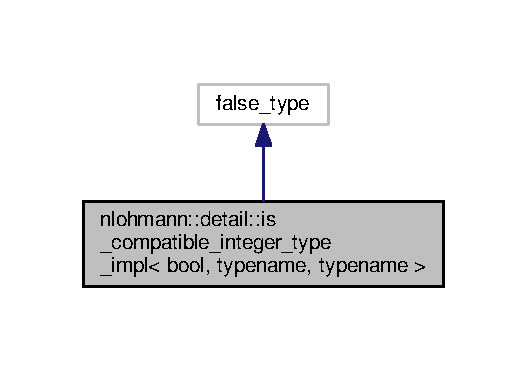
\includegraphics[width=253pt]{structnlohmann_1_1detail_1_1is__compatible__integer__type__impl__inherit__graph}
\end{center}
\end{figure}


Collaboration diagram for nlohmann\+:\+:detail\+:\+:is\+\_\+compatible\+\_\+integer\+\_\+type\+\_\+impl$<$ bool, typename, typename $>$\+:\nopagebreak
\begin{figure}[H]
\begin{center}
\leavevmode
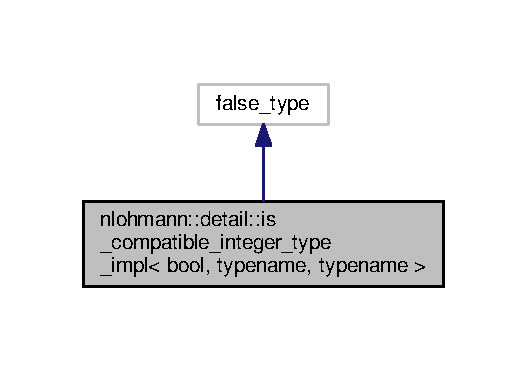
\includegraphics[width=253pt]{structnlohmann_1_1detail_1_1is__compatible__integer__type__impl__coll__graph}
\end{center}
\end{figure}


\subsection{Detailed Description}
\subsubsection*{template$<$bool, typename, typename$>$\\*
struct nlohmann\+::detail\+::is\+\_\+compatible\+\_\+integer\+\_\+type\+\_\+impl$<$ bool, typename, typename $>$}



Definition at line 782 of file json.\+hpp.



The documentation for this struct was generated from the following file\+:\begin{DoxyCompactItemize}
\item 
include/\hyperlink{json_8hpp}{json.\+hpp}\end{DoxyCompactItemize}

\hypertarget{structnlohmann_1_1detail_1_1is__compatible__integer__type__impl_3_01true_00_01_real_integer_type78b0ba77f36a8c8169cdb79b01d1a4bf}{}\section{nlohmann\+:\+:detail\+:\+:is\+\_\+compatible\+\_\+integer\+\_\+type\+\_\+impl$<$ true, Real\+Integer\+Type, Compatible\+Number\+Integer\+Type $>$ Struct Template Reference}
\label{structnlohmann_1_1detail_1_1is__compatible__integer__type__impl_3_01true_00_01_real_integer_type78b0ba77f36a8c8169cdb79b01d1a4bf}\index{nlohmann\+::detail\+::is\+\_\+compatible\+\_\+integer\+\_\+type\+\_\+impl$<$ true, Real\+Integer\+Type, Compatible\+Number\+Integer\+Type $>$@{nlohmann\+::detail\+::is\+\_\+compatible\+\_\+integer\+\_\+type\+\_\+impl$<$ true, Real\+Integer\+Type, Compatible\+Number\+Integer\+Type $>$}}


{\ttfamily \#include $<$json.\+hpp$>$}

\subsection*{Public Types}
\begin{DoxyCompactItemize}
\item 
using \hyperlink{structnlohmann_1_1detail_1_1is__compatible__integer__type__impl_3_01true_00_01_real_integer_type78b0ba77f36a8c8169cdb79b01d1a4bf_a1bad172320cd124997a3d68990f50a75}{Real\+Limits} = std\+::numeric\+\_\+limits$<$ Real\+Integer\+Type $>$
\item 
using \hyperlink{structnlohmann_1_1detail_1_1is__compatible__integer__type__impl_3_01true_00_01_real_integer_type78b0ba77f36a8c8169cdb79b01d1a4bf_a3bf8ee2f76e74f997258c9ba40c64bc4}{Compatible\+Limits} = std\+::numeric\+\_\+limits$<$ Compatible\+Number\+Integer\+Type $>$
\end{DoxyCompactItemize}
\subsection*{Static Public Attributes}
\begin{DoxyCompactItemize}
\item 
static constexpr auto \hyperlink{structnlohmann_1_1detail_1_1is__compatible__integer__type__impl_3_01true_00_01_real_integer_type78b0ba77f36a8c8169cdb79b01d1a4bf_a4c27142452b43418b1d5c0aad01bff50}{value}
\end{DoxyCompactItemize}


\subsection{Detailed Description}
\subsubsection*{template$<$typename Real\+Integer\+Type, typename Compatible\+Number\+Integer\+Type$>$\\*
struct nlohmann\+::detail\+::is\+\_\+compatible\+\_\+integer\+\_\+type\+\_\+impl$<$ true, Real\+Integer\+Type, Compatible\+Number\+Integer\+Type $>$}



Definition at line 785 of file json.\+hpp.



\subsection{Member Typedef Documentation}
\index{nlohmann\+::detail\+::is\+\_\+compatible\+\_\+integer\+\_\+type\+\_\+impl$<$ true, Real\+Integer\+Type, Compatible\+Number\+Integer\+Type $>$@{nlohmann\+::detail\+::is\+\_\+compatible\+\_\+integer\+\_\+type\+\_\+impl$<$ true, Real\+Integer\+Type, Compatible\+Number\+Integer\+Type $>$}!Compatible\+Limits@{Compatible\+Limits}}
\index{Compatible\+Limits@{Compatible\+Limits}!nlohmann\+::detail\+::is\+\_\+compatible\+\_\+integer\+\_\+type\+\_\+impl$<$ true, Real\+Integer\+Type, Compatible\+Number\+Integer\+Type $>$@{nlohmann\+::detail\+::is\+\_\+compatible\+\_\+integer\+\_\+type\+\_\+impl$<$ true, Real\+Integer\+Type, Compatible\+Number\+Integer\+Type $>$}}
\subsubsection[{\texorpdfstring{Compatible\+Limits}{CompatibleLimits}}]{\setlength{\rightskip}{0pt plus 5cm}template$<$typename Real\+Integer\+Type , typename Compatible\+Number\+Integer\+Type $>$ using {\bf nlohmann\+::detail\+::is\+\_\+compatible\+\_\+integer\+\_\+type\+\_\+impl}$<$ true, Real\+Integer\+Type, Compatible\+Number\+Integer\+Type $>$\+::{\bf Compatible\+Limits} =  std\+::numeric\+\_\+limits$<$Compatible\+Number\+Integer\+Type$>$}\hypertarget{structnlohmann_1_1detail_1_1is__compatible__integer__type__impl_3_01true_00_01_real_integer_type78b0ba77f36a8c8169cdb79b01d1a4bf_a3bf8ee2f76e74f997258c9ba40c64bc4}{}\label{structnlohmann_1_1detail_1_1is__compatible__integer__type__impl_3_01true_00_01_real_integer_type78b0ba77f36a8c8169cdb79b01d1a4bf_a3bf8ee2f76e74f997258c9ba40c64bc4}


Definition at line 789 of file json.\+hpp.

\index{nlohmann\+::detail\+::is\+\_\+compatible\+\_\+integer\+\_\+type\+\_\+impl$<$ true, Real\+Integer\+Type, Compatible\+Number\+Integer\+Type $>$@{nlohmann\+::detail\+::is\+\_\+compatible\+\_\+integer\+\_\+type\+\_\+impl$<$ true, Real\+Integer\+Type, Compatible\+Number\+Integer\+Type $>$}!Real\+Limits@{Real\+Limits}}
\index{Real\+Limits@{Real\+Limits}!nlohmann\+::detail\+::is\+\_\+compatible\+\_\+integer\+\_\+type\+\_\+impl$<$ true, Real\+Integer\+Type, Compatible\+Number\+Integer\+Type $>$@{nlohmann\+::detail\+::is\+\_\+compatible\+\_\+integer\+\_\+type\+\_\+impl$<$ true, Real\+Integer\+Type, Compatible\+Number\+Integer\+Type $>$}}
\subsubsection[{\texorpdfstring{Real\+Limits}{RealLimits}}]{\setlength{\rightskip}{0pt plus 5cm}template$<$typename Real\+Integer\+Type , typename Compatible\+Number\+Integer\+Type $>$ using {\bf nlohmann\+::detail\+::is\+\_\+compatible\+\_\+integer\+\_\+type\+\_\+impl}$<$ true, Real\+Integer\+Type, Compatible\+Number\+Integer\+Type $>$\+::{\bf Real\+Limits} =  std\+::numeric\+\_\+limits$<$Real\+Integer\+Type$>$}\hypertarget{structnlohmann_1_1detail_1_1is__compatible__integer__type__impl_3_01true_00_01_real_integer_type78b0ba77f36a8c8169cdb79b01d1a4bf_a1bad172320cd124997a3d68990f50a75}{}\label{structnlohmann_1_1detail_1_1is__compatible__integer__type__impl_3_01true_00_01_real_integer_type78b0ba77f36a8c8169cdb79b01d1a4bf_a1bad172320cd124997a3d68990f50a75}


Definition at line 788 of file json.\+hpp.



\subsection{Member Data Documentation}
\index{nlohmann\+::detail\+::is\+\_\+compatible\+\_\+integer\+\_\+type\+\_\+impl$<$ true, Real\+Integer\+Type, Compatible\+Number\+Integer\+Type $>$@{nlohmann\+::detail\+::is\+\_\+compatible\+\_\+integer\+\_\+type\+\_\+impl$<$ true, Real\+Integer\+Type, Compatible\+Number\+Integer\+Type $>$}!value@{value}}
\index{value@{value}!nlohmann\+::detail\+::is\+\_\+compatible\+\_\+integer\+\_\+type\+\_\+impl$<$ true, Real\+Integer\+Type, Compatible\+Number\+Integer\+Type $>$@{nlohmann\+::detail\+::is\+\_\+compatible\+\_\+integer\+\_\+type\+\_\+impl$<$ true, Real\+Integer\+Type, Compatible\+Number\+Integer\+Type $>$}}
\subsubsection[{\texorpdfstring{value}{value}}]{\setlength{\rightskip}{0pt plus 5cm}template$<$typename Real\+Integer\+Type , typename Compatible\+Number\+Integer\+Type $>$ constexpr auto {\bf nlohmann\+::detail\+::is\+\_\+compatible\+\_\+integer\+\_\+type\+\_\+impl}$<$ true, Real\+Integer\+Type, Compatible\+Number\+Integer\+Type $>$\+::value\hspace{0.3cm}{\ttfamily [static]}}\hypertarget{structnlohmann_1_1detail_1_1is__compatible__integer__type__impl_3_01true_00_01_real_integer_type78b0ba77f36a8c8169cdb79b01d1a4bf_a4c27142452b43418b1d5c0aad01bff50}{}\label{structnlohmann_1_1detail_1_1is__compatible__integer__type__impl_3_01true_00_01_real_integer_type78b0ba77f36a8c8169cdb79b01d1a4bf_a4c27142452b43418b1d5c0aad01bff50}
{\bfseries Initial value\+:}
\begin{DoxyCode}
=
        std::is\_constructible<RealIntegerType, CompatibleNumberIntegerType>::value and
        CompatibleLimits::is\_integer and
        RealLimits::is\_signed == CompatibleLimits::is\_signed
\end{DoxyCode}


Definition at line 791 of file json.\+hpp.



The documentation for this struct was generated from the following file\+:\begin{DoxyCompactItemize}
\item 
include/\hyperlink{json_8hpp}{json.\+hpp}\end{DoxyCompactItemize}

\hypertarget{structnlohmann_1_1detail_1_1is__compatible__object__type}{}\section{nlohmann\+:\+:detail\+:\+:is\+\_\+compatible\+\_\+object\+\_\+type$<$ Basic\+Json\+Type, Compatible\+Object\+Type $>$ Struct Template Reference}
\label{structnlohmann_1_1detail_1_1is__compatible__object__type}\index{nlohmann\+::detail\+::is\+\_\+compatible\+\_\+object\+\_\+type$<$ Basic\+Json\+Type, Compatible\+Object\+Type $>$@{nlohmann\+::detail\+::is\+\_\+compatible\+\_\+object\+\_\+type$<$ Basic\+Json\+Type, Compatible\+Object\+Type $>$}}


{\ttfamily \#include $<$json.\+hpp$>$}

\subsection*{Static Public Attributes}
\begin{DoxyCompactItemize}
\item 
static auto constexpr \hyperlink{structnlohmann_1_1detail_1_1is__compatible__object__type_a87cce7bcdcd22cc8517f171705f6a7c7}{value}
\end{DoxyCompactItemize}


\subsection{Detailed Description}
\subsubsection*{template$<$class Basic\+Json\+Type, class Compatible\+Object\+Type$>$\\*
struct nlohmann\+::detail\+::is\+\_\+compatible\+\_\+object\+\_\+type$<$ Basic\+Json\+Type, Compatible\+Object\+Type $>$}



Definition at line 749 of file json.\+hpp.



\subsection{Member Data Documentation}
\index{nlohmann\+::detail\+::is\+\_\+compatible\+\_\+object\+\_\+type@{nlohmann\+::detail\+::is\+\_\+compatible\+\_\+object\+\_\+type}!value@{value}}
\index{value@{value}!nlohmann\+::detail\+::is\+\_\+compatible\+\_\+object\+\_\+type@{nlohmann\+::detail\+::is\+\_\+compatible\+\_\+object\+\_\+type}}
\subsubsection[{\texorpdfstring{value}{value}}]{\setlength{\rightskip}{0pt plus 5cm}template$<$class Basic\+Json\+Type , class Compatible\+Object\+Type $>$ auto constexpr {\bf nlohmann\+::detail\+::is\+\_\+compatible\+\_\+object\+\_\+type}$<$ Basic\+Json\+Type, Compatible\+Object\+Type $>$\+::value\hspace{0.3cm}{\ttfamily [static]}}\hypertarget{structnlohmann_1_1detail_1_1is__compatible__object__type_a87cce7bcdcd22cc8517f171705f6a7c7}{}\label{structnlohmann_1_1detail_1_1is__compatible__object__type_a87cce7bcdcd22cc8517f171705f6a7c7}
{\bfseries Initial value\+:}
\begin{DoxyCode}
= is\_compatible\_object\_type\_impl <
                                  conjunction<negation<std::is\_same<void, CompatibleObjectType>>,
                                  has\_mapped\_type<CompatibleObjectType>,
                                  has\_key\_type<CompatibleObjectType>>\hyperlink{structnlohmann_1_1detail_1_1is__compatible__object__type_a87cce7bcdcd22cc8517f171705f6a7c7}{::value},
                                  \textcolor{keyword}{typename} BasicJsonType::object\_t, CompatibleObjectType >
      \hyperlink{structnlohmann_1_1detail_1_1is__compatible__object__type_a87cce7bcdcd22cc8517f171705f6a7c7}{::value}
\end{DoxyCode}


Definition at line 751 of file json.\+hpp.



The documentation for this struct was generated from the following file\+:\begin{DoxyCompactItemize}
\item 
include/\hyperlink{json_8hpp}{json.\+hpp}\end{DoxyCompactItemize}

\hypertarget{structnlohmann_1_1detail_1_1is__compatible__object__type__impl}{}\section{nlohmann\+:\+:detail\+:\+:is\+\_\+compatible\+\_\+object\+\_\+type\+\_\+impl$<$ B, Real\+Type, Compatible\+Object\+Type $>$ Struct Template Reference}
\label{structnlohmann_1_1detail_1_1is__compatible__object__type__impl}\index{nlohmann\+::detail\+::is\+\_\+compatible\+\_\+object\+\_\+type\+\_\+impl$<$ B, Real\+Type, Compatible\+Object\+Type $>$@{nlohmann\+::detail\+::is\+\_\+compatible\+\_\+object\+\_\+type\+\_\+impl$<$ B, Real\+Type, Compatible\+Object\+Type $>$}}


{\ttfamily \#include $<$json.\+hpp$>$}



Inheritance diagram for nlohmann\+:\+:detail\+:\+:is\+\_\+compatible\+\_\+object\+\_\+type\+\_\+impl$<$ B, Real\+Type, Compatible\+Object\+Type $>$\+:\nopagebreak
\begin{figure}[H]
\begin{center}
\leavevmode
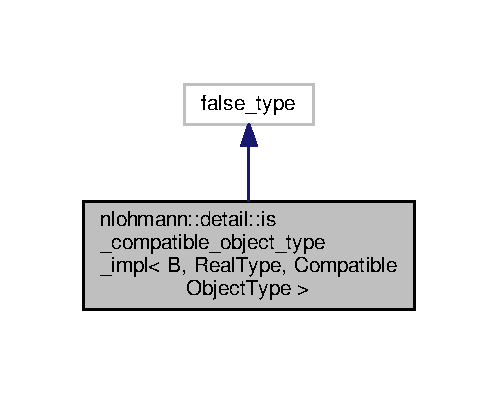
\includegraphics[width=239pt]{structnlohmann_1_1detail_1_1is__compatible__object__type__impl__inherit__graph}
\end{center}
\end{figure}


Collaboration diagram for nlohmann\+:\+:detail\+:\+:is\+\_\+compatible\+\_\+object\+\_\+type\+\_\+impl$<$ B, Real\+Type, Compatible\+Object\+Type $>$\+:\nopagebreak
\begin{figure}[H]
\begin{center}
\leavevmode
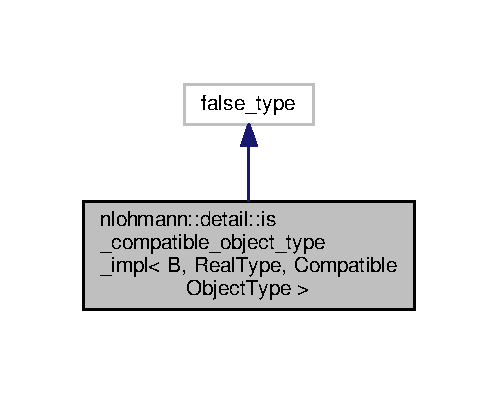
\includegraphics[width=239pt]{structnlohmann_1_1detail_1_1is__compatible__object__type__impl__coll__graph}
\end{center}
\end{figure}


\subsection{Detailed Description}
\subsubsection*{template$<$bool B, class Real\+Type, class Compatible\+Object\+Type$>$\\*
struct nlohmann\+::detail\+::is\+\_\+compatible\+\_\+object\+\_\+type\+\_\+impl$<$ B, Real\+Type, Compatible\+Object\+Type $>$}



Definition at line 738 of file json.\+hpp.



The documentation for this struct was generated from the following file\+:\begin{DoxyCompactItemize}
\item 
include/\hyperlink{json_8hpp}{json.\+hpp}\end{DoxyCompactItemize}

\hypertarget{structnlohmann_1_1detail_1_1is__compatible__object__type__impl_3_01true_00_01_real_type_00_01_compatible_object_type_01_4}{}\section{nlohmann\+:\+:detail\+:\+:is\+\_\+compatible\+\_\+object\+\_\+type\+\_\+impl$<$ true, Real\+Type, Compatible\+Object\+Type $>$ Struct Template Reference}
\label{structnlohmann_1_1detail_1_1is__compatible__object__type__impl_3_01true_00_01_real_type_00_01_compatible_object_type_01_4}\index{nlohmann\+::detail\+::is\+\_\+compatible\+\_\+object\+\_\+type\+\_\+impl$<$ true, Real\+Type, Compatible\+Object\+Type $>$@{nlohmann\+::detail\+::is\+\_\+compatible\+\_\+object\+\_\+type\+\_\+impl$<$ true, Real\+Type, Compatible\+Object\+Type $>$}}


{\ttfamily \#include $<$json.\+hpp$>$}

\subsection*{Static Public Attributes}
\begin{DoxyCompactItemize}
\item 
static constexpr auto \hyperlink{structnlohmann_1_1detail_1_1is__compatible__object__type__impl_3_01true_00_01_real_type_00_01_compatible_object_type_01_4_afa131fcd3a4fc1881dd350a04589e6cf}{value}
\end{DoxyCompactItemize}


\subsection{Detailed Description}
\subsubsection*{template$<$class Real\+Type, class Compatible\+Object\+Type$>$\\*
struct nlohmann\+::detail\+::is\+\_\+compatible\+\_\+object\+\_\+type\+\_\+impl$<$ true, Real\+Type, Compatible\+Object\+Type $>$}



Definition at line 741 of file json.\+hpp.



\subsection{Member Data Documentation}
\index{nlohmann\+::detail\+::is\+\_\+compatible\+\_\+object\+\_\+type\+\_\+impl$<$ true, Real\+Type, Compatible\+Object\+Type $>$@{nlohmann\+::detail\+::is\+\_\+compatible\+\_\+object\+\_\+type\+\_\+impl$<$ true, Real\+Type, Compatible\+Object\+Type $>$}!value@{value}}
\index{value@{value}!nlohmann\+::detail\+::is\+\_\+compatible\+\_\+object\+\_\+type\+\_\+impl$<$ true, Real\+Type, Compatible\+Object\+Type $>$@{nlohmann\+::detail\+::is\+\_\+compatible\+\_\+object\+\_\+type\+\_\+impl$<$ true, Real\+Type, Compatible\+Object\+Type $>$}}
\subsubsection[{\texorpdfstring{value}{value}}]{\setlength{\rightskip}{0pt plus 5cm}template$<$class Real\+Type , class Compatible\+Object\+Type $>$ constexpr auto {\bf nlohmann\+::detail\+::is\+\_\+compatible\+\_\+object\+\_\+type\+\_\+impl}$<$ true, Real\+Type, Compatible\+Object\+Type $>$\+::value\hspace{0.3cm}{\ttfamily [static]}}\hypertarget{structnlohmann_1_1detail_1_1is__compatible__object__type__impl_3_01true_00_01_real_type_00_01_compatible_object_type_01_4_afa131fcd3a4fc1881dd350a04589e6cf}{}\label{structnlohmann_1_1detail_1_1is__compatible__object__type__impl_3_01true_00_01_real_type_00_01_compatible_object_type_01_4_afa131fcd3a4fc1881dd350a04589e6cf}
{\bfseries Initial value\+:}
\begin{DoxyCode}
=
        std::is\_constructible<typename RealType::key\_type, typename CompatibleObjectType::key\_type>::value 
      and
        std::is\_constructible<typename RealType::mapped\_type, typename
       CompatibleObjectType::mapped\_type>::value
\end{DoxyCode}


Definition at line 743 of file json.\+hpp.



The documentation for this struct was generated from the following file\+:\begin{DoxyCompactItemize}
\item 
include/\hyperlink{json_8hpp}{json.\+hpp}\end{DoxyCompactItemize}

\hypertarget{classnlohmann_1_1detail_1_1iter__impl}{}\section{nlohmann\+:\+:detail\+:\+:iter\+\_\+impl$<$ Basic\+Json\+Type $>$ Class Template Reference}
\label{classnlohmann_1_1detail_1_1iter__impl}\index{nlohmann\+::detail\+::iter\+\_\+impl$<$ Basic\+Json\+Type $>$@{nlohmann\+::detail\+::iter\+\_\+impl$<$ Basic\+Json\+Type $>$}}


a template for a random access iterator for the \hyperlink{classnlohmann_1_1basic__json}{basic\+\_\+json} class  




{\ttfamily \#include $<$json.\+hpp$>$}



Inheritance diagram for nlohmann\+:\+:detail\+:\+:iter\+\_\+impl$<$ Basic\+Json\+Type $>$\+:\nopagebreak
\begin{figure}[H]
\begin{center}
\leavevmode
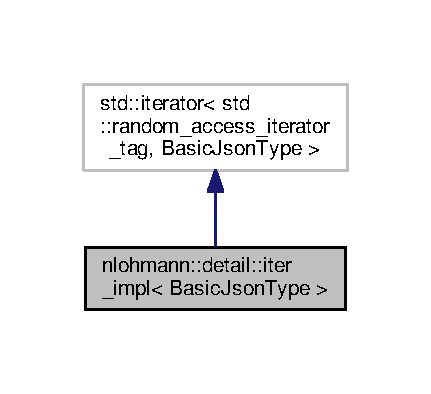
\includegraphics[width=207pt]{classnlohmann_1_1detail_1_1iter__impl__inherit__graph}
\end{center}
\end{figure}


Collaboration diagram for nlohmann\+:\+:detail\+:\+:iter\+\_\+impl$<$ Basic\+Json\+Type $>$\+:\nopagebreak
\begin{figure}[H]
\begin{center}
\leavevmode
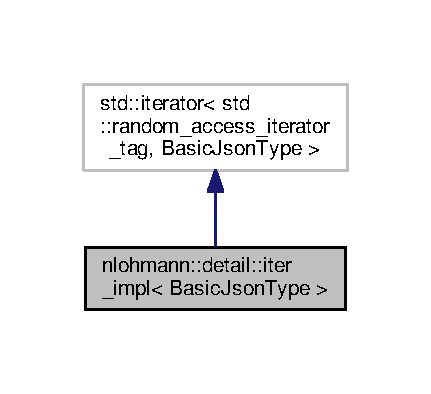
\includegraphics[width=207pt]{classnlohmann_1_1detail_1_1iter__impl__coll__graph}
\end{center}
\end{figure}
\subsection*{Public Types}
\begin{DoxyCompactItemize}
\item 
using \hyperlink{classnlohmann_1_1detail_1_1iter__impl_ab35586a44f2222272c5346baa3013f67}{value\+\_\+type} = typename Basic\+Json\+Type\+::value\+\_\+type
\begin{DoxyCompactList}\small\item\em the type of the values when the iterator is dereferenced \end{DoxyCompactList}\item 
using \hyperlink{classnlohmann_1_1detail_1_1iter__impl_a2f7ea9f7022850809c60fc3263775840}{difference\+\_\+type} = typename Basic\+Json\+Type\+::difference\+\_\+type
\begin{DoxyCompactList}\small\item\em a type to represent differences between iterators \end{DoxyCompactList}\item 
using \hyperlink{classnlohmann_1_1detail_1_1iter__impl_a69e52f890ce8c556fd68ce109e24b360}{pointer} = typename std\+::conditional$<$ std\+::is\+\_\+const$<$ Basic\+Json\+Type $>$\+::\hyperlink{classnlohmann_1_1detail_1_1iter__impl_adc4048d25e057ce8ec0b912642c24731}{value}, typename Basic\+Json\+Type\+::const\+\_\+pointer, typename Basic\+Json\+Type\+::pointer $>$\+::type
\begin{DoxyCompactList}\small\item\em defines a pointer to the type iterated over (value\+\_\+type) \end{DoxyCompactList}\item 
using \hyperlink{classnlohmann_1_1detail_1_1iter__impl_a5be8001be099c6b82310f4d387b953ce}{reference} = typename std\+::conditional$<$ std\+::is\+\_\+const$<$ Basic\+Json\+Type $>$\+::\hyperlink{classnlohmann_1_1detail_1_1iter__impl_adc4048d25e057ce8ec0b912642c24731}{value}, typename Basic\+Json\+Type\+::const\+\_\+reference, typename Basic\+Json\+Type\+::reference $>$\+::type
\begin{DoxyCompactList}\small\item\em defines a reference to the type iterated over (value\+\_\+type) \end{DoxyCompactList}\item 
using \hyperlink{classnlohmann_1_1detail_1_1iter__impl_ad9e091f5c70b34b5b1abc1ab15fd9106}{iterator\+\_\+category} = std\+::bidirectional\+\_\+iterator\+\_\+tag
\begin{DoxyCompactList}\small\item\em the category of the iterator \end{DoxyCompactList}\end{DoxyCompactItemize}
\subsection*{Public Member Functions}
\begin{DoxyCompactItemize}
\item 
\hyperlink{classnlohmann_1_1detail_1_1iter__impl_a19aa457f9c4af1b7e3af59839132cc5c}{iter\+\_\+impl} ()=default
\begin{DoxyCompactList}\small\item\em default constructor \end{DoxyCompactList}\item 
\hyperlink{classnlohmann_1_1detail_1_1iter__impl_a88a00484ac201c52fc5f613d88a2918b}{iter\+\_\+impl} (\hyperlink{classnlohmann_1_1detail_1_1iter__impl_a69e52f890ce8c556fd68ce109e24b360}{pointer} \hyperlink{namespacenlohmann_1_1detail_a90aa5ef615aa8305e9ea20d8a947980faa8cfde6331bd59eb2ac96f8911c4b666}{object}) noexcept
\begin{DoxyCompactList}\small\item\em constructor for a given J\+S\+ON instance \end{DoxyCompactList}\item 
\hyperlink{classnlohmann_1_1detail_1_1iter__impl_a867f7eb55091be31b013adb3e46816d3}{iter\+\_\+impl} (const \hyperlink{classnlohmann_1_1detail_1_1iter__impl}{iter\+\_\+impl}$<$ typename std\+::remove\+\_\+const$<$ Basic\+Json\+Type $>$\+::type $>$ \&other) noexcept
\begin{DoxyCompactList}\small\item\em converting constructor \end{DoxyCompactList}\item 
\hyperlink{classnlohmann_1_1detail_1_1iter__impl}{iter\+\_\+impl} \& \hyperlink{classnlohmann_1_1detail_1_1iter__impl_a7159ed1cfe7c423a2baef8bea0c94509}{operator=} (const \hyperlink{classnlohmann_1_1detail_1_1iter__impl}{iter\+\_\+impl}$<$ typename std\+::remove\+\_\+const$<$ Basic\+Json\+Type $>$\+::type $>$ \&other) noexcept
\begin{DoxyCompactList}\small\item\em converting assignment \end{DoxyCompactList}\item 
\hyperlink{classnlohmann_1_1detail_1_1iter__impl_a5be8001be099c6b82310f4d387b953ce}{reference} \hyperlink{classnlohmann_1_1detail_1_1iter__impl_adafa65198cad0cc7295d21cfa7678e6e}{operator$\ast$} () const 
\begin{DoxyCompactList}\small\item\em return a reference to the value pointed to by the iterator \end{DoxyCompactList}\item 
\hyperlink{classnlohmann_1_1detail_1_1iter__impl_a69e52f890ce8c556fd68ce109e24b360}{pointer} \hyperlink{classnlohmann_1_1detail_1_1iter__impl_a28a0c92903edd8f86825c8c7784b0913}{operator-\/$>$} () const 
\begin{DoxyCompactList}\small\item\em dereference the iterator \end{DoxyCompactList}\item 
\hyperlink{classnlohmann_1_1detail_1_1iter__impl}{iter\+\_\+impl} \hyperlink{classnlohmann_1_1detail_1_1iter__impl_ae64452217b17567717039a158f8bc029}{operator++} (int)
\begin{DoxyCompactList}\small\item\em post-\/increment (it++) \end{DoxyCompactList}\item 
\hyperlink{classnlohmann_1_1detail_1_1iter__impl}{iter\+\_\+impl} \& \hyperlink{classnlohmann_1_1detail_1_1iter__impl_abdfe2a7f464400a7ab572782d14b922f}{operator++} ()
\begin{DoxyCompactList}\small\item\em pre-\/increment (++it) \end{DoxyCompactList}\item 
\hyperlink{classnlohmann_1_1detail_1_1iter__impl}{iter\+\_\+impl} \hyperlink{classnlohmann_1_1detail_1_1iter__impl_ab8479a4395bb0ab3661d842a9ee47767}{operator-\/-\/} (int)
\begin{DoxyCompactList}\small\item\em post-\/decrement (it--) \end{DoxyCompactList}\item 
\hyperlink{classnlohmann_1_1detail_1_1iter__impl}{iter\+\_\+impl} \& \hyperlink{classnlohmann_1_1detail_1_1iter__impl_a84e689fb581d651d130039f7cb81494a}{operator-\/-\/} ()
\begin{DoxyCompactList}\small\item\em pre-\/decrement (--it) \end{DoxyCompactList}\item 
bool \hyperlink{classnlohmann_1_1detail_1_1iter__impl_abe91c77d1be747fadcbfaf6f685e3ee7}{operator==} (const \hyperlink{classnlohmann_1_1detail_1_1iter__impl}{iter\+\_\+impl} \&other) const 
\begin{DoxyCompactList}\small\item\em comparison\+: equal \end{DoxyCompactList}\item 
bool \hyperlink{classnlohmann_1_1detail_1_1iter__impl_a66af27bbbf9743bc000264a0f89c5d0d}{operator!=} (const \hyperlink{classnlohmann_1_1detail_1_1iter__impl}{iter\+\_\+impl} \&other) const 
\begin{DoxyCompactList}\small\item\em comparison\+: not equal \end{DoxyCompactList}\item 
bool \hyperlink{classnlohmann_1_1detail_1_1iter__impl_a3a5123a4cfe72a9d674c9ff65c4ec08c}{operator$<$} (const \hyperlink{classnlohmann_1_1detail_1_1iter__impl}{iter\+\_\+impl} \&other) const 
\begin{DoxyCompactList}\small\item\em comparison\+: smaller \end{DoxyCompactList}\item 
bool \hyperlink{classnlohmann_1_1detail_1_1iter__impl_aa90b4d1da290b5073778e295dc2985f3}{operator$<$=} (const \hyperlink{classnlohmann_1_1detail_1_1iter__impl}{iter\+\_\+impl} \&other) const 
\begin{DoxyCompactList}\small\item\em comparison\+: less than or equal \end{DoxyCompactList}\item 
bool \hyperlink{classnlohmann_1_1detail_1_1iter__impl_afe8894bea0a0b616d9d5975ca04e8b39}{operator$>$} (const \hyperlink{classnlohmann_1_1detail_1_1iter__impl}{iter\+\_\+impl} \&other) const 
\begin{DoxyCompactList}\small\item\em comparison\+: greater than \end{DoxyCompactList}\item 
bool \hyperlink{classnlohmann_1_1detail_1_1iter__impl_ae87ea99999c169722b388c69871295e3}{operator$>$=} (const \hyperlink{classnlohmann_1_1detail_1_1iter__impl}{iter\+\_\+impl} \&other) const 
\begin{DoxyCompactList}\small\item\em comparison\+: greater than or equal \end{DoxyCompactList}\item 
\hyperlink{classnlohmann_1_1detail_1_1iter__impl}{iter\+\_\+impl} \& \hyperlink{classnlohmann_1_1detail_1_1iter__impl_a3eef94f9d167046e7f773aeb6b78090c}{operator+=} (\hyperlink{classnlohmann_1_1detail_1_1iter__impl_a2f7ea9f7022850809c60fc3263775840}{difference\+\_\+type} i)
\begin{DoxyCompactList}\small\item\em add to iterator \end{DoxyCompactList}\item 
\hyperlink{classnlohmann_1_1detail_1_1iter__impl}{iter\+\_\+impl} \& \hyperlink{classnlohmann_1_1detail_1_1iter__impl_abcc9d51bc52f2e8483bbe4018f05e978}{operator-\/=} (\hyperlink{classnlohmann_1_1detail_1_1iter__impl_a2f7ea9f7022850809c60fc3263775840}{difference\+\_\+type} i)
\begin{DoxyCompactList}\small\item\em subtract from iterator \end{DoxyCompactList}\item 
\hyperlink{classnlohmann_1_1detail_1_1iter__impl}{iter\+\_\+impl} \hyperlink{classnlohmann_1_1detail_1_1iter__impl_afc5629527a820583cd009c411e30ac64}{operator+} (\hyperlink{classnlohmann_1_1detail_1_1iter__impl_a2f7ea9f7022850809c60fc3263775840}{difference\+\_\+type} i) const 
\begin{DoxyCompactList}\small\item\em add to iterator \end{DoxyCompactList}\item 
\hyperlink{classnlohmann_1_1detail_1_1iter__impl}{iter\+\_\+impl} \hyperlink{classnlohmann_1_1detail_1_1iter__impl_aa719903e6d509db51744cfca9c95fd8e}{operator-\/} (\hyperlink{classnlohmann_1_1detail_1_1iter__impl_a2f7ea9f7022850809c60fc3263775840}{difference\+\_\+type} i) const 
\begin{DoxyCompactList}\small\item\em subtract from iterator \end{DoxyCompactList}\item 
\hyperlink{classnlohmann_1_1detail_1_1iter__impl_a2f7ea9f7022850809c60fc3263775840}{difference\+\_\+type} \hyperlink{classnlohmann_1_1detail_1_1iter__impl_a327f3f6a97c6d0cdfc9fe232949d916b}{operator-\/} (const \hyperlink{classnlohmann_1_1detail_1_1iter__impl}{iter\+\_\+impl} \&other) const 
\begin{DoxyCompactList}\small\item\em return difference \end{DoxyCompactList}\item 
\hyperlink{classnlohmann_1_1detail_1_1iter__impl_a5be8001be099c6b82310f4d387b953ce}{reference} \hyperlink{classnlohmann_1_1detail_1_1iter__impl_ade15572ccb7c5b9c2541ecfd65252e99}{operator\mbox{[}$\,$\mbox{]}} (\hyperlink{classnlohmann_1_1detail_1_1iter__impl_a2f7ea9f7022850809c60fc3263775840}{difference\+\_\+type} n) const 
\begin{DoxyCompactList}\small\item\em access to successor \end{DoxyCompactList}\item 
object\+\_\+t\+::key\+\_\+type \hyperlink{classnlohmann_1_1detail_1_1iter__impl_aa2e9909148c4df211d89a0a8608e556c}{key} () const 
\begin{DoxyCompactList}\small\item\em return the key of an object iterator \end{DoxyCompactList}\item 
\hyperlink{classnlohmann_1_1detail_1_1iter__impl_a5be8001be099c6b82310f4d387b953ce}{reference} \hyperlink{classnlohmann_1_1detail_1_1iter__impl_adc4048d25e057ce8ec0b912642c24731}{value} () const 
\begin{DoxyCompactList}\small\item\em return the value of an iterator \end{DoxyCompactList}\end{DoxyCompactItemize}
\subsection*{Friends}
\begin{DoxyCompactItemize}
\item 
\hyperlink{classnlohmann_1_1detail_1_1iter__impl}{iter\+\_\+impl} \hyperlink{classnlohmann_1_1detail_1_1iter__impl_a94108d1a7563e103534f23eb5c1ee175}{operator+} (\hyperlink{classnlohmann_1_1detail_1_1iter__impl_a2f7ea9f7022850809c60fc3263775840}{difference\+\_\+type} i, const \hyperlink{classnlohmann_1_1detail_1_1iter__impl}{iter\+\_\+impl} \&it)
\begin{DoxyCompactList}\small\item\em addition of distance and iterator \end{DoxyCompactList}\end{DoxyCompactItemize}


\subsection{Detailed Description}
\subsubsection*{template$<$typename Basic\+Json\+Type$>$\\*
class nlohmann\+::detail\+::iter\+\_\+impl$<$ Basic\+Json\+Type $>$}

a template for a random access iterator for the \hyperlink{classnlohmann_1_1basic__json}{basic\+\_\+json} class 

This class implements a both iterators (iterator and const\+\_\+iterator) for the \hyperlink{classnlohmann_1_1basic__json}{basic\+\_\+json} class.

\begin{DoxyNote}{Note}
An iterator is called {\itshape initialized} when a pointer to a J\+S\+ON value has been set (e.\+g., by a constructor or a copy assignment). If the iterator is default-\/constructed, it is {\itshape uninitialized} and most methods are undefined. The library uses assertions to detect calls on uninitialized iterators.$\ast$$\ast$
\end{DoxyNote}
The class satisfies the following concept requirements\+:
\begin{DoxyItemize}
\item \href{http://en.cppreference.com/w/cpp/concept/RandomAccessIterator}{\tt Random\+Access\+Iterator}\+: The iterator that can be moved to point (forward and backward) to any element in constant time.
\end{DoxyItemize}

\begin{DoxySince}{Since}
version 1.\+0.\+0, simplified in version 2.\+0.\+9 
\end{DoxySince}


Definition at line 3556 of file json.\+hpp.



\subsection{Member Typedef Documentation}
\index{nlohmann\+::detail\+::iter\+\_\+impl@{nlohmann\+::detail\+::iter\+\_\+impl}!difference\+\_\+type@{difference\+\_\+type}}
\index{difference\+\_\+type@{difference\+\_\+type}!nlohmann\+::detail\+::iter\+\_\+impl@{nlohmann\+::detail\+::iter\+\_\+impl}}
\subsubsection[{\texorpdfstring{difference\+\_\+type}{difference_type}}]{\setlength{\rightskip}{0pt plus 5cm}template$<$typename Basic\+Json\+Type$>$ using {\bf nlohmann\+::detail\+::iter\+\_\+impl}$<$ Basic\+Json\+Type $>$\+::{\bf difference\+\_\+type} =  typename Basic\+Json\+Type\+::difference\+\_\+type}\hypertarget{classnlohmann_1_1detail_1_1iter__impl_a2f7ea9f7022850809c60fc3263775840}{}\label{classnlohmann_1_1detail_1_1iter__impl_a2f7ea9f7022850809c60fc3263775840}


a type to represent differences between iterators 



Definition at line 3573 of file json.\+hpp.

\index{nlohmann\+::detail\+::iter\+\_\+impl@{nlohmann\+::detail\+::iter\+\_\+impl}!iterator\+\_\+category@{iterator\+\_\+category}}
\index{iterator\+\_\+category@{iterator\+\_\+category}!nlohmann\+::detail\+::iter\+\_\+impl@{nlohmann\+::detail\+::iter\+\_\+impl}}
\subsubsection[{\texorpdfstring{iterator\+\_\+category}{iterator_category}}]{\setlength{\rightskip}{0pt plus 5cm}template$<$typename Basic\+Json\+Type$>$ using {\bf nlohmann\+::detail\+::iter\+\_\+impl}$<$ Basic\+Json\+Type $>$\+::{\bf iterator\+\_\+category} =  std\+::bidirectional\+\_\+iterator\+\_\+tag}\hypertarget{classnlohmann_1_1detail_1_1iter__impl_ad9e091f5c70b34b5b1abc1ab15fd9106}{}\label{classnlohmann_1_1detail_1_1iter__impl_ad9e091f5c70b34b5b1abc1ab15fd9106}


the category of the iterator 



Definition at line 3584 of file json.\+hpp.

\index{nlohmann\+::detail\+::iter\+\_\+impl@{nlohmann\+::detail\+::iter\+\_\+impl}!pointer@{pointer}}
\index{pointer@{pointer}!nlohmann\+::detail\+::iter\+\_\+impl@{nlohmann\+::detail\+::iter\+\_\+impl}}
\subsubsection[{\texorpdfstring{pointer}{pointer}}]{\setlength{\rightskip}{0pt plus 5cm}template$<$typename Basic\+Json\+Type$>$ using {\bf nlohmann\+::detail\+::iter\+\_\+impl}$<$ Basic\+Json\+Type $>$\+::{\bf pointer} =  typename std\+::conditional$<$std\+::is\+\_\+const$<$Basic\+Json\+Type$>$\+::{\bf value}, typename Basic\+Json\+Type\+::const\+\_\+pointer, typename Basic\+Json\+Type\+::pointer$>$\+::type}\hypertarget{classnlohmann_1_1detail_1_1iter__impl_a69e52f890ce8c556fd68ce109e24b360}{}\label{classnlohmann_1_1detail_1_1iter__impl_a69e52f890ce8c556fd68ce109e24b360}


defines a pointer to the type iterated over (value\+\_\+type) 



Definition at line 3577 of file json.\+hpp.

\index{nlohmann\+::detail\+::iter\+\_\+impl@{nlohmann\+::detail\+::iter\+\_\+impl}!reference@{reference}}
\index{reference@{reference}!nlohmann\+::detail\+::iter\+\_\+impl@{nlohmann\+::detail\+::iter\+\_\+impl}}
\subsubsection[{\texorpdfstring{reference}{reference}}]{\setlength{\rightskip}{0pt plus 5cm}template$<$typename Basic\+Json\+Type$>$ using {\bf nlohmann\+::detail\+::iter\+\_\+impl}$<$ Basic\+Json\+Type $>$\+::{\bf reference} =  typename std\+::conditional$<$std\+::is\+\_\+const$<$Basic\+Json\+Type$>$\+::{\bf value}, typename Basic\+Json\+Type\+::const\+\_\+reference, typename Basic\+Json\+Type\+::reference$>$\+::type}\hypertarget{classnlohmann_1_1detail_1_1iter__impl_a5be8001be099c6b82310f4d387b953ce}{}\label{classnlohmann_1_1detail_1_1iter__impl_a5be8001be099c6b82310f4d387b953ce}


defines a reference to the type iterated over (value\+\_\+type) 



Definition at line 3582 of file json.\+hpp.

\index{nlohmann\+::detail\+::iter\+\_\+impl@{nlohmann\+::detail\+::iter\+\_\+impl}!value\+\_\+type@{value\+\_\+type}}
\index{value\+\_\+type@{value\+\_\+type}!nlohmann\+::detail\+::iter\+\_\+impl@{nlohmann\+::detail\+::iter\+\_\+impl}}
\subsubsection[{\texorpdfstring{value\+\_\+type}{value_type}}]{\setlength{\rightskip}{0pt plus 5cm}template$<$typename Basic\+Json\+Type$>$ using {\bf nlohmann\+::detail\+::iter\+\_\+impl}$<$ Basic\+Json\+Type $>$\+::{\bf value\+\_\+type} =  typename Basic\+Json\+Type\+::value\+\_\+type}\hypertarget{classnlohmann_1_1detail_1_1iter__impl_ab35586a44f2222272c5346baa3013f67}{}\label{classnlohmann_1_1detail_1_1iter__impl_ab35586a44f2222272c5346baa3013f67}


the type of the values when the iterator is dereferenced 



Definition at line 3571 of file json.\+hpp.



\subsection{Constructor \& Destructor Documentation}
\index{nlohmann\+::detail\+::iter\+\_\+impl@{nlohmann\+::detail\+::iter\+\_\+impl}!iter\+\_\+impl@{iter\+\_\+impl}}
\index{iter\+\_\+impl@{iter\+\_\+impl}!nlohmann\+::detail\+::iter\+\_\+impl@{nlohmann\+::detail\+::iter\+\_\+impl}}
\subsubsection[{\texorpdfstring{iter\+\_\+impl()=default}{iter_impl()=default}}]{\setlength{\rightskip}{0pt plus 5cm}template$<$typename Basic\+Json\+Type$>$ {\bf iter\+\_\+impl}$<$ typename std\+::conditional$<$ std\+::is\+\_\+const$<$ Basic\+Json\+Type $>$\+::{\bf value}, typename std\+::remove\+\_\+const$<$ Basic\+Json\+Type $>$\+::type, const Basic\+Json\+Type $>$\+::type $>$ (
\begin{DoxyParamCaption}
{}
\end{DoxyParamCaption}
)\hspace{0.3cm}{\ttfamily [default]}}\hypertarget{classnlohmann_1_1detail_1_1iter__impl_a19aa457f9c4af1b7e3af59839132cc5c}{}\label{classnlohmann_1_1detail_1_1iter__impl_a19aa457f9c4af1b7e3af59839132cc5c}


default constructor 

allow \hyperlink{classnlohmann_1_1basic__json}{basic\+\_\+json} to access private members 

Definition at line 3559 of file json.\+hpp.

\index{nlohmann\+::detail\+::iter\+\_\+impl@{nlohmann\+::detail\+::iter\+\_\+impl}!iter\+\_\+impl@{iter\+\_\+impl}}
\index{iter\+\_\+impl@{iter\+\_\+impl}!nlohmann\+::detail\+::iter\+\_\+impl@{nlohmann\+::detail\+::iter\+\_\+impl}}
\subsubsection[{\texorpdfstring{iter\+\_\+impl(pointer object) noexcept}{iter_impl(pointer object) noexcept}}]{\setlength{\rightskip}{0pt plus 5cm}template$<$typename Basic\+Json\+Type$>$ {\bf nlohmann\+::detail\+::iter\+\_\+impl}$<$ Basic\+Json\+Type $>$\+::{\bf iter\+\_\+impl} (
\begin{DoxyParamCaption}
\item[{{\bf pointer}}]{object}
\end{DoxyParamCaption}
)\hspace{0.3cm}{\ttfamily [inline]}, {\ttfamily [explicit]}, {\ttfamily [noexcept]}}\hypertarget{classnlohmann_1_1detail_1_1iter__impl_a88a00484ac201c52fc5f613d88a2918b}{}\label{classnlohmann_1_1detail_1_1iter__impl_a88a00484ac201c52fc5f613d88a2918b}


constructor for a given J\+S\+ON instance 


\begin{DoxyParams}[1]{Parameters}
\mbox{\tt in}  & {\em object} & pointer to a J\+S\+ON object for this iterator \\
\hline
\end{DoxyParams}
\begin{DoxyPrecond}{Precondition}
object != nullptr 
\end{DoxyPrecond}
\begin{DoxyPostcond}{Postcondition}
The iterator is initialized; i.\+e. {\ttfamily m\+\_\+object != nullptr}. 
\end{DoxyPostcond}


Definition at line 3595 of file json.\+hpp.

\index{nlohmann\+::detail\+::iter\+\_\+impl@{nlohmann\+::detail\+::iter\+\_\+impl}!iter\+\_\+impl@{iter\+\_\+impl}}
\index{iter\+\_\+impl@{iter\+\_\+impl}!nlohmann\+::detail\+::iter\+\_\+impl@{nlohmann\+::detail\+::iter\+\_\+impl}}
\subsubsection[{\texorpdfstring{iter\+\_\+impl(const iter\+\_\+impl$<$ typename std\+::remove\+\_\+const$<$ Basic\+Json\+Type $>$\+::type $>$ \&other) noexcept}{iter_impl(const iter_impl< typename std::remove_const< BasicJsonType >::type > &other) noexcept}}]{\setlength{\rightskip}{0pt plus 5cm}template$<$typename Basic\+Json\+Type$>$ {\bf nlohmann\+::detail\+::iter\+\_\+impl}$<$ Basic\+Json\+Type $>$\+::{\bf iter\+\_\+impl} (
\begin{DoxyParamCaption}
\item[{const {\bf iter\+\_\+impl}$<$ typename std\+::remove\+\_\+const$<$ Basic\+Json\+Type $>$\+::type $>$ \&}]{other}
\end{DoxyParamCaption}
)\hspace{0.3cm}{\ttfamily [inline]}, {\ttfamily [noexcept]}}\hypertarget{classnlohmann_1_1detail_1_1iter__impl_a867f7eb55091be31b013adb3e46816d3}{}\label{classnlohmann_1_1detail_1_1iter__impl_a867f7eb55091be31b013adb3e46816d3}


converting constructor 

\begin{DoxyNote}{Note}
The conventional copy constructor and copy assignment are implicitly defined. Combined with the following converting constructor and assignment, they support\+: (1) copy from iterator to iterator, (2) copy from const iterator to const iterator, and (3) conversion from iterator to const iterator. However conversion from const iterator to iterator is not defined.
\end{DoxyNote}

\begin{DoxyParams}[1]{Parameters}
\mbox{\tt in}  & {\em other} & non-\/const iterator to copy from \\
\hline
\end{DoxyParams}
\begin{DoxyNote}{Note}
It is not checked whether {\itshape other} is initialized. 
\end{DoxyNote}


Definition at line 3635 of file json.\+hpp.



\subsection{Member Function Documentation}
\index{nlohmann\+::detail\+::iter\+\_\+impl@{nlohmann\+::detail\+::iter\+\_\+impl}!key@{key}}
\index{key@{key}!nlohmann\+::detail\+::iter\+\_\+impl@{nlohmann\+::detail\+::iter\+\_\+impl}}
\subsubsection[{\texorpdfstring{key() const }{key() const }}]{\setlength{\rightskip}{0pt plus 5cm}template$<$typename Basic\+Json\+Type$>$ object\+\_\+t\+::key\+\_\+type {\bf nlohmann\+::detail\+::iter\+\_\+impl}$<$ Basic\+Json\+Type $>$\+::key (
\begin{DoxyParamCaption}
{}
\end{DoxyParamCaption}
) const\hspace{0.3cm}{\ttfamily [inline]}}\hypertarget{classnlohmann_1_1detail_1_1iter__impl_aa2e9909148c4df211d89a0a8608e556c}{}\label{classnlohmann_1_1detail_1_1iter__impl_aa2e9909148c4df211d89a0a8608e556c}


return the key of an object iterator 

\begin{DoxyPrecond}{Precondition}
The iterator is initialized; i.\+e. {\ttfamily m\+\_\+object != nullptr}. 
\end{DoxyPrecond}


Definition at line 4122 of file json.\+hpp.

\index{nlohmann\+::detail\+::iter\+\_\+impl@{nlohmann\+::detail\+::iter\+\_\+impl}!operator"!=@{operator"!=}}
\index{operator"!=@{operator"!=}!nlohmann\+::detail\+::iter\+\_\+impl@{nlohmann\+::detail\+::iter\+\_\+impl}}
\subsubsection[{\texorpdfstring{operator"!=(const iter\+\_\+impl \&other) const }{operator!=(const iter_impl &other) const }}]{\setlength{\rightskip}{0pt plus 5cm}template$<$typename Basic\+Json\+Type$>$ bool {\bf nlohmann\+::detail\+::iter\+\_\+impl}$<$ Basic\+Json\+Type $>$\+::operator!= (
\begin{DoxyParamCaption}
\item[{const {\bf iter\+\_\+impl}$<$ Basic\+Json\+Type $>$ \&}]{other}
\end{DoxyParamCaption}
) const\hspace{0.3cm}{\ttfamily [inline]}}\hypertarget{classnlohmann_1_1detail_1_1iter__impl_a66af27bbbf9743bc000264a0f89c5d0d}{}\label{classnlohmann_1_1detail_1_1iter__impl_a66af27bbbf9743bc000264a0f89c5d0d}


comparison\+: not equal 

\begin{DoxyPrecond}{Precondition}
The iterator is initialized; i.\+e. {\ttfamily m\+\_\+object != nullptr}. 
\end{DoxyPrecond}


Definition at line 3916 of file json.\+hpp.

\index{nlohmann\+::detail\+::iter\+\_\+impl@{nlohmann\+::detail\+::iter\+\_\+impl}!operator$\ast$@{operator$\ast$}}
\index{operator$\ast$@{operator$\ast$}!nlohmann\+::detail\+::iter\+\_\+impl@{nlohmann\+::detail\+::iter\+\_\+impl}}
\subsubsection[{\texorpdfstring{operator$\ast$() const }{operator*() const }}]{\setlength{\rightskip}{0pt plus 5cm}template$<$typename Basic\+Json\+Type$>$ {\bf reference} {\bf nlohmann\+::detail\+::iter\+\_\+impl}$<$ Basic\+Json\+Type $>$\+::operator$\ast$ (
\begin{DoxyParamCaption}
{}
\end{DoxyParamCaption}
) const\hspace{0.3cm}{\ttfamily [inline]}}\hypertarget{classnlohmann_1_1detail_1_1iter__impl_adafa65198cad0cc7295d21cfa7678e6e}{}\label{classnlohmann_1_1detail_1_1iter__impl_adafa65198cad0cc7295d21cfa7678e6e}


return a reference to the value pointed to by the iterator 

\begin{DoxyPrecond}{Precondition}
The iterator is initialized; i.\+e. {\ttfamily m\+\_\+object != nullptr}. 
\end{DoxyPrecond}


Definition at line 3724 of file json.\+hpp.

\index{nlohmann\+::detail\+::iter\+\_\+impl@{nlohmann\+::detail\+::iter\+\_\+impl}!operator+@{operator+}}
\index{operator+@{operator+}!nlohmann\+::detail\+::iter\+\_\+impl@{nlohmann\+::detail\+::iter\+\_\+impl}}
\subsubsection[{\texorpdfstring{operator+(difference\+\_\+type i) const }{operator+(difference_type i) const }}]{\setlength{\rightskip}{0pt plus 5cm}template$<$typename Basic\+Json\+Type$>$ {\bf iter\+\_\+impl} {\bf nlohmann\+::detail\+::iter\+\_\+impl}$<$ Basic\+Json\+Type $>$\+::operator+ (
\begin{DoxyParamCaption}
\item[{{\bf difference\+\_\+type}}]{i}
\end{DoxyParamCaption}
) const\hspace{0.3cm}{\ttfamily [inline]}}\hypertarget{classnlohmann_1_1detail_1_1iter__impl_afc5629527a820583cd009c411e30ac64}{}\label{classnlohmann_1_1detail_1_1iter__impl_afc5629527a820583cd009c411e30ac64}


add to iterator 

\begin{DoxyPrecond}{Precondition}
The iterator is initialized; i.\+e. {\ttfamily m\+\_\+object != nullptr}. 
\end{DoxyPrecond}


Definition at line 4025 of file json.\+hpp.

\index{nlohmann\+::detail\+::iter\+\_\+impl@{nlohmann\+::detail\+::iter\+\_\+impl}!operator++@{operator++}}
\index{operator++@{operator++}!nlohmann\+::detail\+::iter\+\_\+impl@{nlohmann\+::detail\+::iter\+\_\+impl}}
\subsubsection[{\texorpdfstring{operator++(int)}{operator++(int)}}]{\setlength{\rightskip}{0pt plus 5cm}template$<$typename Basic\+Json\+Type$>$ {\bf iter\+\_\+impl} {\bf nlohmann\+::detail\+::iter\+\_\+impl}$<$ Basic\+Json\+Type $>$\+::operator++ (
\begin{DoxyParamCaption}
\item[{int}]{}
\end{DoxyParamCaption}
)\hspace{0.3cm}{\ttfamily [inline]}}\hypertarget{classnlohmann_1_1detail_1_1iter__impl_ae64452217b17567717039a158f8bc029}{}\label{classnlohmann_1_1detail_1_1iter__impl_ae64452217b17567717039a158f8bc029}


post-\/increment (it++) 

\begin{DoxyPrecond}{Precondition}
The iterator is initialized; i.\+e. {\ttfamily m\+\_\+object != nullptr}. 
\end{DoxyPrecond}


Definition at line 3797 of file json.\+hpp.

\index{nlohmann\+::detail\+::iter\+\_\+impl@{nlohmann\+::detail\+::iter\+\_\+impl}!operator++@{operator++}}
\index{operator++@{operator++}!nlohmann\+::detail\+::iter\+\_\+impl@{nlohmann\+::detail\+::iter\+\_\+impl}}
\subsubsection[{\texorpdfstring{operator++()}{operator++()}}]{\setlength{\rightskip}{0pt plus 5cm}template$<$typename Basic\+Json\+Type$>$ {\bf iter\+\_\+impl}\& {\bf nlohmann\+::detail\+::iter\+\_\+impl}$<$ Basic\+Json\+Type $>$\+::operator++ (
\begin{DoxyParamCaption}
{}
\end{DoxyParamCaption}
)\hspace{0.3cm}{\ttfamily [inline]}}\hypertarget{classnlohmann_1_1detail_1_1iter__impl_abdfe2a7f464400a7ab572782d14b922f}{}\label{classnlohmann_1_1detail_1_1iter__impl_abdfe2a7f464400a7ab572782d14b922f}


pre-\/increment (++it) 

\begin{DoxyPrecond}{Precondition}
The iterator is initialized; i.\+e. {\ttfamily m\+\_\+object != nullptr}. 
\end{DoxyPrecond}


Definition at line 3808 of file json.\+hpp.

\index{nlohmann\+::detail\+::iter\+\_\+impl@{nlohmann\+::detail\+::iter\+\_\+impl}!operator+=@{operator+=}}
\index{operator+=@{operator+=}!nlohmann\+::detail\+::iter\+\_\+impl@{nlohmann\+::detail\+::iter\+\_\+impl}}
\subsubsection[{\texorpdfstring{operator+=(difference\+\_\+type i)}{operator+=(difference_type i)}}]{\setlength{\rightskip}{0pt plus 5cm}template$<$typename Basic\+Json\+Type$>$ {\bf iter\+\_\+impl}\& {\bf nlohmann\+::detail\+::iter\+\_\+impl}$<$ Basic\+Json\+Type $>$\+::operator+= (
\begin{DoxyParamCaption}
\item[{{\bf difference\+\_\+type}}]{i}
\end{DoxyParamCaption}
)\hspace{0.3cm}{\ttfamily [inline]}}\hypertarget{classnlohmann_1_1detail_1_1iter__impl_a3eef94f9d167046e7f773aeb6b78090c}{}\label{classnlohmann_1_1detail_1_1iter__impl_a3eef94f9d167046e7f773aeb6b78090c}


add to iterator 

\begin{DoxyPrecond}{Precondition}
The iterator is initialized; i.\+e. {\ttfamily m\+\_\+object != nullptr}. 
\end{DoxyPrecond}


Definition at line 3985 of file json.\+hpp.

\index{nlohmann\+::detail\+::iter\+\_\+impl@{nlohmann\+::detail\+::iter\+\_\+impl}!operator-\/@{operator-\/}}
\index{operator-\/@{operator-\/}!nlohmann\+::detail\+::iter\+\_\+impl@{nlohmann\+::detail\+::iter\+\_\+impl}}
\subsubsection[{\texorpdfstring{operator-\/(difference\+\_\+type i) const }{operator-(difference_type i) const }}]{\setlength{\rightskip}{0pt plus 5cm}template$<$typename Basic\+Json\+Type$>$ {\bf iter\+\_\+impl} {\bf nlohmann\+::detail\+::iter\+\_\+impl}$<$ Basic\+Json\+Type $>$\+::operator-\/ (
\begin{DoxyParamCaption}
\item[{{\bf difference\+\_\+type}}]{i}
\end{DoxyParamCaption}
) const\hspace{0.3cm}{\ttfamily [inline]}}\hypertarget{classnlohmann_1_1detail_1_1iter__impl_aa719903e6d509db51744cfca9c95fd8e}{}\label{classnlohmann_1_1detail_1_1iter__impl_aa719903e6d509db51744cfca9c95fd8e}


subtract from iterator 

\begin{DoxyPrecond}{Precondition}
The iterator is initialized; i.\+e. {\ttfamily m\+\_\+object != nullptr}. 
\end{DoxyPrecond}


Definition at line 4047 of file json.\+hpp.

\index{nlohmann\+::detail\+::iter\+\_\+impl@{nlohmann\+::detail\+::iter\+\_\+impl}!operator-\/@{operator-\/}}
\index{operator-\/@{operator-\/}!nlohmann\+::detail\+::iter\+\_\+impl@{nlohmann\+::detail\+::iter\+\_\+impl}}
\subsubsection[{\texorpdfstring{operator-\/(const iter\+\_\+impl \&other) const }{operator-(const iter_impl &other) const }}]{\setlength{\rightskip}{0pt plus 5cm}template$<$typename Basic\+Json\+Type$>$ {\bf difference\+\_\+type} {\bf nlohmann\+::detail\+::iter\+\_\+impl}$<$ Basic\+Json\+Type $>$\+::operator-\/ (
\begin{DoxyParamCaption}
\item[{const {\bf iter\+\_\+impl}$<$ Basic\+Json\+Type $>$ \&}]{other}
\end{DoxyParamCaption}
) const\hspace{0.3cm}{\ttfamily [inline]}}\hypertarget{classnlohmann_1_1detail_1_1iter__impl_a327f3f6a97c6d0cdfc9fe232949d916b}{}\label{classnlohmann_1_1detail_1_1iter__impl_a327f3f6a97c6d0cdfc9fe232949d916b}


return difference 

\begin{DoxyPrecond}{Precondition}
The iterator is initialized; i.\+e. {\ttfamily m\+\_\+object != nullptr}. 
\end{DoxyPrecond}


Definition at line 4058 of file json.\+hpp.

\index{nlohmann\+::detail\+::iter\+\_\+impl@{nlohmann\+::detail\+::iter\+\_\+impl}!operator-\/-\/@{operator-\/-\/}}
\index{operator-\/-\/@{operator-\/-\/}!nlohmann\+::detail\+::iter\+\_\+impl@{nlohmann\+::detail\+::iter\+\_\+impl}}
\subsubsection[{\texorpdfstring{operator-\/-\/(int)}{operator--(int)}}]{\setlength{\rightskip}{0pt plus 5cm}template$<$typename Basic\+Json\+Type$>$ {\bf iter\+\_\+impl} {\bf nlohmann\+::detail\+::iter\+\_\+impl}$<$ Basic\+Json\+Type $>$\+::operator-\/-\/ (
\begin{DoxyParamCaption}
\item[{int}]{}
\end{DoxyParamCaption}
)\hspace{0.3cm}{\ttfamily [inline]}}\hypertarget{classnlohmann_1_1detail_1_1iter__impl_ab8479a4395bb0ab3661d842a9ee47767}{}\label{classnlohmann_1_1detail_1_1iter__impl_ab8479a4395bb0ab3661d842a9ee47767}


post-\/decrement (it--) 

\begin{DoxyPrecond}{Precondition}
The iterator is initialized; i.\+e. {\ttfamily m\+\_\+object != nullptr}. 
\end{DoxyPrecond}


Definition at line 3840 of file json.\+hpp.

\index{nlohmann\+::detail\+::iter\+\_\+impl@{nlohmann\+::detail\+::iter\+\_\+impl}!operator-\/-\/@{operator-\/-\/}}
\index{operator-\/-\/@{operator-\/-\/}!nlohmann\+::detail\+::iter\+\_\+impl@{nlohmann\+::detail\+::iter\+\_\+impl}}
\subsubsection[{\texorpdfstring{operator-\/-\/()}{operator--()}}]{\setlength{\rightskip}{0pt plus 5cm}template$<$typename Basic\+Json\+Type$>$ {\bf iter\+\_\+impl}\& {\bf nlohmann\+::detail\+::iter\+\_\+impl}$<$ Basic\+Json\+Type $>$\+::operator-\/-\/ (
\begin{DoxyParamCaption}
{}
\end{DoxyParamCaption}
)\hspace{0.3cm}{\ttfamily [inline]}}\hypertarget{classnlohmann_1_1detail_1_1iter__impl_a84e689fb581d651d130039f7cb81494a}{}\label{classnlohmann_1_1detail_1_1iter__impl_a84e689fb581d651d130039f7cb81494a}


pre-\/decrement (--it) 

\begin{DoxyPrecond}{Precondition}
The iterator is initialized; i.\+e. {\ttfamily m\+\_\+object != nullptr}. 
\end{DoxyPrecond}


Definition at line 3851 of file json.\+hpp.

\index{nlohmann\+::detail\+::iter\+\_\+impl@{nlohmann\+::detail\+::iter\+\_\+impl}!operator-\/=@{operator-\/=}}
\index{operator-\/=@{operator-\/=}!nlohmann\+::detail\+::iter\+\_\+impl@{nlohmann\+::detail\+::iter\+\_\+impl}}
\subsubsection[{\texorpdfstring{operator-\/=(difference\+\_\+type i)}{operator-=(difference_type i)}}]{\setlength{\rightskip}{0pt plus 5cm}template$<$typename Basic\+Json\+Type$>$ {\bf iter\+\_\+impl}\& {\bf nlohmann\+::detail\+::iter\+\_\+impl}$<$ Basic\+Json\+Type $>$\+::operator-\/= (
\begin{DoxyParamCaption}
\item[{{\bf difference\+\_\+type}}]{i}
\end{DoxyParamCaption}
)\hspace{0.3cm}{\ttfamily [inline]}}\hypertarget{classnlohmann_1_1detail_1_1iter__impl_abcc9d51bc52f2e8483bbe4018f05e978}{}\label{classnlohmann_1_1detail_1_1iter__impl_abcc9d51bc52f2e8483bbe4018f05e978}


subtract from iterator 

\begin{DoxyPrecond}{Precondition}
The iterator is initialized; i.\+e. {\ttfamily m\+\_\+object != nullptr}. 
\end{DoxyPrecond}


Definition at line 4016 of file json.\+hpp.

\index{nlohmann\+::detail\+::iter\+\_\+impl@{nlohmann\+::detail\+::iter\+\_\+impl}!operator-\/$>$@{operator-\/$>$}}
\index{operator-\/$>$@{operator-\/$>$}!nlohmann\+::detail\+::iter\+\_\+impl@{nlohmann\+::detail\+::iter\+\_\+impl}}
\subsubsection[{\texorpdfstring{operator-\/$>$() const }{operator->() const }}]{\setlength{\rightskip}{0pt plus 5cm}template$<$typename Basic\+Json\+Type$>$ {\bf pointer} {\bf nlohmann\+::detail\+::iter\+\_\+impl}$<$ Basic\+Json\+Type $>$\+::operator-\/$>$ (
\begin{DoxyParamCaption}
{}
\end{DoxyParamCaption}
) const\hspace{0.3cm}{\ttfamily [inline]}}\hypertarget{classnlohmann_1_1detail_1_1iter__impl_a28a0c92903edd8f86825c8c7784b0913}{}\label{classnlohmann_1_1detail_1_1iter__impl_a28a0c92903edd8f86825c8c7784b0913}


dereference the iterator 

\begin{DoxyPrecond}{Precondition}
The iterator is initialized; i.\+e. {\ttfamily m\+\_\+object != nullptr}. 
\end{DoxyPrecond}


Definition at line 3763 of file json.\+hpp.

\index{nlohmann\+::detail\+::iter\+\_\+impl@{nlohmann\+::detail\+::iter\+\_\+impl}!operator$<$@{operator$<$}}
\index{operator$<$@{operator$<$}!nlohmann\+::detail\+::iter\+\_\+impl@{nlohmann\+::detail\+::iter\+\_\+impl}}
\subsubsection[{\texorpdfstring{operator$<$(const iter\+\_\+impl \&other) const }{operator<(const iter_impl &other) const }}]{\setlength{\rightskip}{0pt plus 5cm}template$<$typename Basic\+Json\+Type$>$ bool {\bf nlohmann\+::detail\+::iter\+\_\+impl}$<$ Basic\+Json\+Type $>$\+::operator$<$ (
\begin{DoxyParamCaption}
\item[{const {\bf iter\+\_\+impl}$<$ Basic\+Json\+Type $>$ \&}]{other}
\end{DoxyParamCaption}
) const\hspace{0.3cm}{\ttfamily [inline]}}\hypertarget{classnlohmann_1_1detail_1_1iter__impl_a3a5123a4cfe72a9d674c9ff65c4ec08c}{}\label{classnlohmann_1_1detail_1_1iter__impl_a3a5123a4cfe72a9d674c9ff65c4ec08c}


comparison\+: smaller 

\begin{DoxyPrecond}{Precondition}
The iterator is initialized; i.\+e. {\ttfamily m\+\_\+object != nullptr}. 
\end{DoxyPrecond}


Definition at line 3925 of file json.\+hpp.

\index{nlohmann\+::detail\+::iter\+\_\+impl@{nlohmann\+::detail\+::iter\+\_\+impl}!operator$<$=@{operator$<$=}}
\index{operator$<$=@{operator$<$=}!nlohmann\+::detail\+::iter\+\_\+impl@{nlohmann\+::detail\+::iter\+\_\+impl}}
\subsubsection[{\texorpdfstring{operator$<$=(const iter\+\_\+impl \&other) const }{operator<=(const iter_impl &other) const }}]{\setlength{\rightskip}{0pt plus 5cm}template$<$typename Basic\+Json\+Type$>$ bool {\bf nlohmann\+::detail\+::iter\+\_\+impl}$<$ Basic\+Json\+Type $>$\+::operator$<$= (
\begin{DoxyParamCaption}
\item[{const {\bf iter\+\_\+impl}$<$ Basic\+Json\+Type $>$ \&}]{other}
\end{DoxyParamCaption}
) const\hspace{0.3cm}{\ttfamily [inline]}}\hypertarget{classnlohmann_1_1detail_1_1iter__impl_aa90b4d1da290b5073778e295dc2985f3}{}\label{classnlohmann_1_1detail_1_1iter__impl_aa90b4d1da290b5073778e295dc2985f3}


comparison\+: less than or equal 

\begin{DoxyPrecond}{Precondition}
The iterator is initialized; i.\+e. {\ttfamily m\+\_\+object != nullptr}. 
\end{DoxyPrecond}


Definition at line 3958 of file json.\+hpp.

\index{nlohmann\+::detail\+::iter\+\_\+impl@{nlohmann\+::detail\+::iter\+\_\+impl}!operator=@{operator=}}
\index{operator=@{operator=}!nlohmann\+::detail\+::iter\+\_\+impl@{nlohmann\+::detail\+::iter\+\_\+impl}}
\subsubsection[{\texorpdfstring{operator=(const iter\+\_\+impl$<$ typename std\+::remove\+\_\+const$<$ Basic\+Json\+Type $>$\+::type $>$ \&other) noexcept}{operator=(const iter_impl< typename std::remove_const< BasicJsonType >::type > &other) noexcept}}]{\setlength{\rightskip}{0pt plus 5cm}template$<$typename Basic\+Json\+Type$>$ {\bf iter\+\_\+impl}\& {\bf nlohmann\+::detail\+::iter\+\_\+impl}$<$ Basic\+Json\+Type $>$\+::operator= (
\begin{DoxyParamCaption}
\item[{const {\bf iter\+\_\+impl}$<$ typename std\+::remove\+\_\+const$<$ Basic\+Json\+Type $>$\+::type $>$ \&}]{other}
\end{DoxyParamCaption}
)\hspace{0.3cm}{\ttfamily [inline]}, {\ttfamily [noexcept]}}\hypertarget{classnlohmann_1_1detail_1_1iter__impl_a7159ed1cfe7c423a2baef8bea0c94509}{}\label{classnlohmann_1_1detail_1_1iter__impl_a7159ed1cfe7c423a2baef8bea0c94509}


converting assignment 


\begin{DoxyParams}[1]{Parameters}
\mbox{\tt in,out}  & {\em other} & non-\/const iterator to copy from \\
\hline
\end{DoxyParams}
\begin{DoxyReturn}{Returns}
const/non-\/const iterator 
\end{DoxyReturn}
\begin{DoxyNote}{Note}
It is not checked whether {\itshape other} is initialized. 
\end{DoxyNote}


Definition at line 3644 of file json.\+hpp.

\index{nlohmann\+::detail\+::iter\+\_\+impl@{nlohmann\+::detail\+::iter\+\_\+impl}!operator==@{operator==}}
\index{operator==@{operator==}!nlohmann\+::detail\+::iter\+\_\+impl@{nlohmann\+::detail\+::iter\+\_\+impl}}
\subsubsection[{\texorpdfstring{operator==(const iter\+\_\+impl \&other) const }{operator==(const iter_impl &other) const }}]{\setlength{\rightskip}{0pt plus 5cm}template$<$typename Basic\+Json\+Type$>$ bool {\bf nlohmann\+::detail\+::iter\+\_\+impl}$<$ Basic\+Json\+Type $>$\+::operator== (
\begin{DoxyParamCaption}
\item[{const {\bf iter\+\_\+impl}$<$ Basic\+Json\+Type $>$ \&}]{other}
\end{DoxyParamCaption}
) const\hspace{0.3cm}{\ttfamily [inline]}}\hypertarget{classnlohmann_1_1detail_1_1iter__impl_abe91c77d1be747fadcbfaf6f685e3ee7}{}\label{classnlohmann_1_1detail_1_1iter__impl_abe91c77d1be747fadcbfaf6f685e3ee7}


comparison\+: equal 

\begin{DoxyPrecond}{Precondition}
The iterator is initialized; i.\+e. {\ttfamily m\+\_\+object != nullptr}. 
\end{DoxyPrecond}


Definition at line 3883 of file json.\+hpp.

\index{nlohmann\+::detail\+::iter\+\_\+impl@{nlohmann\+::detail\+::iter\+\_\+impl}!operator$>$@{operator$>$}}
\index{operator$>$@{operator$>$}!nlohmann\+::detail\+::iter\+\_\+impl@{nlohmann\+::detail\+::iter\+\_\+impl}}
\subsubsection[{\texorpdfstring{operator$>$(const iter\+\_\+impl \&other) const }{operator>(const iter_impl &other) const }}]{\setlength{\rightskip}{0pt plus 5cm}template$<$typename Basic\+Json\+Type$>$ bool {\bf nlohmann\+::detail\+::iter\+\_\+impl}$<$ Basic\+Json\+Type $>$\+::operator$>$ (
\begin{DoxyParamCaption}
\item[{const {\bf iter\+\_\+impl}$<$ Basic\+Json\+Type $>$ \&}]{other}
\end{DoxyParamCaption}
) const\hspace{0.3cm}{\ttfamily [inline]}}\hypertarget{classnlohmann_1_1detail_1_1iter__impl_afe8894bea0a0b616d9d5975ca04e8b39}{}\label{classnlohmann_1_1detail_1_1iter__impl_afe8894bea0a0b616d9d5975ca04e8b39}


comparison\+: greater than 

\begin{DoxyPrecond}{Precondition}
The iterator is initialized; i.\+e. {\ttfamily m\+\_\+object != nullptr}. 
\end{DoxyPrecond}


Definition at line 3967 of file json.\+hpp.

\index{nlohmann\+::detail\+::iter\+\_\+impl@{nlohmann\+::detail\+::iter\+\_\+impl}!operator$>$=@{operator$>$=}}
\index{operator$>$=@{operator$>$=}!nlohmann\+::detail\+::iter\+\_\+impl@{nlohmann\+::detail\+::iter\+\_\+impl}}
\subsubsection[{\texorpdfstring{operator$>$=(const iter\+\_\+impl \&other) const }{operator>=(const iter_impl &other) const }}]{\setlength{\rightskip}{0pt plus 5cm}template$<$typename Basic\+Json\+Type$>$ bool {\bf nlohmann\+::detail\+::iter\+\_\+impl}$<$ Basic\+Json\+Type $>$\+::operator$>$= (
\begin{DoxyParamCaption}
\item[{const {\bf iter\+\_\+impl}$<$ Basic\+Json\+Type $>$ \&}]{other}
\end{DoxyParamCaption}
) const\hspace{0.3cm}{\ttfamily [inline]}}\hypertarget{classnlohmann_1_1detail_1_1iter__impl_ae87ea99999c169722b388c69871295e3}{}\label{classnlohmann_1_1detail_1_1iter__impl_ae87ea99999c169722b388c69871295e3}


comparison\+: greater than or equal 

\begin{DoxyPrecond}{Precondition}
The iterator is initialized; i.\+e. {\ttfamily m\+\_\+object != nullptr}. 
\end{DoxyPrecond}


Definition at line 3976 of file json.\+hpp.

\index{nlohmann\+::detail\+::iter\+\_\+impl@{nlohmann\+::detail\+::iter\+\_\+impl}!operator\mbox{[}$\,$\mbox{]}@{operator[]}}
\index{operator\mbox{[}$\,$\mbox{]}@{operator[]}!nlohmann\+::detail\+::iter\+\_\+impl@{nlohmann\+::detail\+::iter\+\_\+impl}}
\subsubsection[{\texorpdfstring{operator[](difference\+\_\+type n) const }{operator[](difference_type n) const }}]{\setlength{\rightskip}{0pt plus 5cm}template$<$typename Basic\+Json\+Type$>$ {\bf reference} {\bf nlohmann\+::detail\+::iter\+\_\+impl}$<$ Basic\+Json\+Type $>$\+::operator\mbox{[}$\,$\mbox{]} (
\begin{DoxyParamCaption}
\item[{{\bf difference\+\_\+type}}]{n}
\end{DoxyParamCaption}
) const\hspace{0.3cm}{\ttfamily [inline]}}\hypertarget{classnlohmann_1_1detail_1_1iter__impl_ade15572ccb7c5b9c2541ecfd65252e99}{}\label{classnlohmann_1_1detail_1_1iter__impl_ade15572ccb7c5b9c2541ecfd65252e99}


access to successor 

\begin{DoxyPrecond}{Precondition}
The iterator is initialized; i.\+e. {\ttfamily m\+\_\+object != nullptr}. 
\end{DoxyPrecond}


Definition at line 4085 of file json.\+hpp.

\index{nlohmann\+::detail\+::iter\+\_\+impl@{nlohmann\+::detail\+::iter\+\_\+impl}!value@{value}}
\index{value@{value}!nlohmann\+::detail\+::iter\+\_\+impl@{nlohmann\+::detail\+::iter\+\_\+impl}}
\subsubsection[{\texorpdfstring{value() const }{value() const }}]{\setlength{\rightskip}{0pt plus 5cm}template$<$typename Basic\+Json\+Type$>$ {\bf reference} {\bf nlohmann\+::detail\+::iter\+\_\+impl}$<$ Basic\+Json\+Type $>$\+::value (
\begin{DoxyParamCaption}
{}
\end{DoxyParamCaption}
) const\hspace{0.3cm}{\ttfamily [inline]}}\hypertarget{classnlohmann_1_1detail_1_1iter__impl_adc4048d25e057ce8ec0b912642c24731}{}\label{classnlohmann_1_1detail_1_1iter__impl_adc4048d25e057ce8ec0b912642c24731}


return the value of an iterator 

\begin{DoxyPrecond}{Precondition}
The iterator is initialized; i.\+e. {\ttfamily m\+\_\+object != nullptr}. 
\end{DoxyPrecond}


Definition at line 4138 of file json.\+hpp.



\subsection{Friends And Related Function Documentation}
\index{nlohmann\+::detail\+::iter\+\_\+impl@{nlohmann\+::detail\+::iter\+\_\+impl}!operator+@{operator+}}
\index{operator+@{operator+}!nlohmann\+::detail\+::iter\+\_\+impl@{nlohmann\+::detail\+::iter\+\_\+impl}}
\subsubsection[{\texorpdfstring{operator+}{operator+}}]{\setlength{\rightskip}{0pt plus 5cm}template$<$typename Basic\+Json\+Type$>$ {\bf iter\+\_\+impl} operator+ (
\begin{DoxyParamCaption}
\item[{{\bf difference\+\_\+type}}]{i, }
\item[{const {\bf iter\+\_\+impl}$<$ Basic\+Json\+Type $>$ \&}]{it}
\end{DoxyParamCaption}
)\hspace{0.3cm}{\ttfamily [friend]}}\hypertarget{classnlohmann_1_1detail_1_1iter__impl_a94108d1a7563e103534f23eb5c1ee175}{}\label{classnlohmann_1_1detail_1_1iter__impl_a94108d1a7563e103534f23eb5c1ee175}


addition of distance and iterator 

\begin{DoxyPrecond}{Precondition}
The iterator is initialized; i.\+e. {\ttfamily m\+\_\+object != nullptr}. 
\end{DoxyPrecond}


Definition at line 4036 of file json.\+hpp.



The documentation for this class was generated from the following file\+:\begin{DoxyCompactItemize}
\item 
include/\hyperlink{json_8hpp}{json.\+hpp}\end{DoxyCompactItemize}

\hypertarget{classnlohmann_1_1detail_1_1iteration__proxy}{}\section{nlohmann\+:\+:detail\+:\+:iteration\+\_\+proxy$<$ Iterator\+Type $>$ Class Template Reference}
\label{classnlohmann_1_1detail_1_1iteration__proxy}\index{nlohmann\+::detail\+::iteration\+\_\+proxy$<$ Iterator\+Type $>$@{nlohmann\+::detail\+::iteration\+\_\+proxy$<$ Iterator\+Type $>$}}


proxy class for the iterator\+\_\+wrapper functions  




{\ttfamily \#include $<$json.\+hpp$>$}

\subsection*{Public Member Functions}
\begin{DoxyCompactItemize}
\item 
\hyperlink{classnlohmann_1_1detail_1_1iteration__proxy_a0aad65238c66bebda98caa9a0002ae1f}{iteration\+\_\+proxy} (typename Iterator\+Type\+::reference cont)
\begin{DoxyCompactList}\small\item\em construct iteration proxy from a container \end{DoxyCompactList}\item 
iteration\+\_\+proxy\+\_\+internal \hyperlink{classnlohmann_1_1detail_1_1iteration__proxy_a43612db469c82118fc648c3729e40cee}{begin} () noexcept
\begin{DoxyCompactList}\small\item\em return iterator begin (needed for range-\/based for) \end{DoxyCompactList}\item 
iteration\+\_\+proxy\+\_\+internal \hyperlink{classnlohmann_1_1detail_1_1iteration__proxy_a41303419d073f32fcf1956978410d816}{end} () noexcept
\begin{DoxyCompactList}\small\item\em return iterator end (needed for range-\/based for) \end{DoxyCompactList}\end{DoxyCompactItemize}


\subsection{Detailed Description}
\subsubsection*{template$<$typename Iterator\+Type$>$\\*
class nlohmann\+::detail\+::iteration\+\_\+proxy$<$ Iterator\+Type $>$}

proxy class for the iterator\+\_\+wrapper functions 

Definition at line 3534 of file json.\+hpp.



\subsection{Constructor \& Destructor Documentation}
\index{nlohmann\+::detail\+::iteration\+\_\+proxy@{nlohmann\+::detail\+::iteration\+\_\+proxy}!iteration\+\_\+proxy@{iteration\+\_\+proxy}}
\index{iteration\+\_\+proxy@{iteration\+\_\+proxy}!nlohmann\+::detail\+::iteration\+\_\+proxy@{nlohmann\+::detail\+::iteration\+\_\+proxy}}
\subsubsection[{\texorpdfstring{iteration\+\_\+proxy(typename Iterator\+Type\+::reference cont)}{iteration_proxy(typename IteratorType::reference cont)}}]{\setlength{\rightskip}{0pt plus 5cm}template$<$typename Iterator\+Type $>$ {\bf nlohmann\+::detail\+::iteration\+\_\+proxy}$<$ Iterator\+Type $>$\+::{\bf iteration\+\_\+proxy} (
\begin{DoxyParamCaption}
\item[{typename Iterator\+Type\+::reference}]{cont}
\end{DoxyParamCaption}
)\hspace{0.3cm}{\ttfamily [inline]}, {\ttfamily [explicit]}}\hypertarget{classnlohmann_1_1detail_1_1iteration__proxy_a0aad65238c66bebda98caa9a0002ae1f}{}\label{classnlohmann_1_1detail_1_1iteration__proxy_a0aad65238c66bebda98caa9a0002ae1f}


construct iteration proxy from a container 



Definition at line 4226 of file json.\+hpp.



\subsection{Member Function Documentation}
\index{nlohmann\+::detail\+::iteration\+\_\+proxy@{nlohmann\+::detail\+::iteration\+\_\+proxy}!begin@{begin}}
\index{begin@{begin}!nlohmann\+::detail\+::iteration\+\_\+proxy@{nlohmann\+::detail\+::iteration\+\_\+proxy}}
\subsubsection[{\texorpdfstring{begin() noexcept}{begin() noexcept}}]{\setlength{\rightskip}{0pt plus 5cm}template$<$typename Iterator\+Type $>$ iteration\+\_\+proxy\+\_\+internal {\bf nlohmann\+::detail\+::iteration\+\_\+proxy}$<$ Iterator\+Type $>$\+::begin (
\begin{DoxyParamCaption}
{}
\end{DoxyParamCaption}
)\hspace{0.3cm}{\ttfamily [inline]}, {\ttfamily [noexcept]}}\hypertarget{classnlohmann_1_1detail_1_1iteration__proxy_a43612db469c82118fc648c3729e40cee}{}\label{classnlohmann_1_1detail_1_1iteration__proxy_a43612db469c82118fc648c3729e40cee}


return iterator begin (needed for range-\/based for) 



Definition at line 4230 of file json.\+hpp.

\index{nlohmann\+::detail\+::iteration\+\_\+proxy@{nlohmann\+::detail\+::iteration\+\_\+proxy}!end@{end}}
\index{end@{end}!nlohmann\+::detail\+::iteration\+\_\+proxy@{nlohmann\+::detail\+::iteration\+\_\+proxy}}
\subsubsection[{\texorpdfstring{end() noexcept}{end() noexcept}}]{\setlength{\rightskip}{0pt plus 5cm}template$<$typename Iterator\+Type $>$ iteration\+\_\+proxy\+\_\+internal {\bf nlohmann\+::detail\+::iteration\+\_\+proxy}$<$ Iterator\+Type $>$\+::end (
\begin{DoxyParamCaption}
{}
\end{DoxyParamCaption}
)\hspace{0.3cm}{\ttfamily [inline]}, {\ttfamily [noexcept]}}\hypertarget{classnlohmann_1_1detail_1_1iteration__proxy_a41303419d073f32fcf1956978410d816}{}\label{classnlohmann_1_1detail_1_1iteration__proxy_a41303419d073f32fcf1956978410d816}


return iterator end (needed for range-\/based for) 



Definition at line 4236 of file json.\+hpp.



The documentation for this class was generated from the following file\+:\begin{DoxyCompactItemize}
\item 
include/\hyperlink{json_8hpp}{json.\+hpp}\end{DoxyCompactItemize}

\hypertarget{classnlohmann_1_1json__pointer}{}\section{nlohmann\+:\+:json\+\_\+pointer Class Reference}
\label{classnlohmann_1_1json__pointer}\index{nlohmann\+::json\+\_\+pointer@{nlohmann\+::json\+\_\+pointer}}


J\+S\+ON Pointer.  




{\ttfamily \#include $<$json.\+hpp$>$}

\subsection*{Public Member Functions}
\begin{DoxyCompactItemize}
\item 
\hyperlink{classnlohmann_1_1json__pointer_a203910314c0be11c6b2b2cb53a9ad3aa}{json\+\_\+pointer} (const std\+::string \&s=\char`\"{}\char`\"{})
\begin{DoxyCompactList}\small\item\em create J\+S\+ON pointer \end{DoxyCompactList}\item 
std\+::string \hyperlink{classnlohmann_1_1json__pointer_a0920ebb015398813880e3c0f8464526e}{to\+\_\+string} () const noexcept
\begin{DoxyCompactList}\small\item\em return a string representation of the J\+S\+ON pointer \end{DoxyCompactList}\item 
\hyperlink{classnlohmann_1_1json__pointer_a63ea79682ed667584d498c901459873a}{operator std\+::string} () const 
\begin{DoxyCompactList}\small\item\em return a string representation of the J\+S\+ON pointer \end{DoxyCompactList}\end{DoxyCompactItemize}
\subsection*{Friends}
\begin{DoxyCompactItemize}
\item 
class \hyperlink{classnlohmann_1_1json__pointer_ada3100cdb8700566051828f1355fa745}{basic\+\_\+json}
\begin{DoxyCompactList}\small\item\em allow \hyperlink{classnlohmann_1_1basic__json}{basic\+\_\+json} to access private members \end{DoxyCompactList}\item 
bool \hyperlink{classnlohmann_1_1json__pointer_a4667ef558c8c3f8a646bfda0c6654653}{operator==} (\hyperlink{classnlohmann_1_1json__pointer}{json\+\_\+pointer} const \&lhs, \hyperlink{classnlohmann_1_1json__pointer}{json\+\_\+pointer} const \&rhs) noexcept
\item 
bool \hyperlink{classnlohmann_1_1json__pointer_a6779edcf28e6f018a3bbb29c0b4b5e1e}{operator!=} (\hyperlink{classnlohmann_1_1json__pointer}{json\+\_\+pointer} const \&lhs, \hyperlink{classnlohmann_1_1json__pointer}{json\+\_\+pointer} const \&rhs) noexcept
\end{DoxyCompactItemize}


\subsection{Detailed Description}
J\+S\+ON Pointer. 

A J\+S\+ON pointer defines a string syntax for identifying a specific value within a J\+S\+ON document. It can be used with functions {\ttfamily at} and {\ttfamily operator\mbox{[}\mbox{]}}. Furthermore, J\+S\+ON pointers are the base for J\+S\+ON patches.

\begin{DoxySeeAlso}{See also}
\href{https://tools.ietf.org/html/rfc6901}{\tt R\+FC 6901}
\end{DoxySeeAlso}
\begin{DoxySince}{Since}
version 2.\+0.\+0 
\end{DoxySince}


Definition at line 6972 of file json.\+hpp.



\subsection{Constructor \& Destructor Documentation}
\index{nlohmann\+::json\+\_\+pointer@{nlohmann\+::json\+\_\+pointer}!json\+\_\+pointer@{json\+\_\+pointer}}
\index{json\+\_\+pointer@{json\+\_\+pointer}!nlohmann\+::json\+\_\+pointer@{nlohmann\+::json\+\_\+pointer}}
\subsubsection[{\texorpdfstring{json\+\_\+pointer(const std\+::string \&s="""")}{json_pointer(const std::string &s="")}}]{\setlength{\rightskip}{0pt plus 5cm}nlohmann\+::json\+\_\+pointer\+::json\+\_\+pointer (
\begin{DoxyParamCaption}
\item[{const std\+::string \&}]{s = {\ttfamily \char`\"{}\char`\"{}}}
\end{DoxyParamCaption}
)\hspace{0.3cm}{\ttfamily [inline]}, {\ttfamily [explicit]}}\hypertarget{classnlohmann_1_1json__pointer_a203910314c0be11c6b2b2cb53a9ad3aa}{}\label{classnlohmann_1_1json__pointer_a203910314c0be11c6b2b2cb53a9ad3aa}


create J\+S\+ON pointer 

Create a J\+S\+ON pointer according to the syntax described in \href{https://tools.ietf.org/html/rfc6901#section-3}{\tt Section 3 of R\+F\+C6901}.


\begin{DoxyParams}[1]{Parameters}
\mbox{\tt in}  & {\em s} & string representing the J\+S\+ON pointer; if omitted, the empty string is assumed which references the whole J\+S\+ON value\\
\hline
\end{DoxyParams}

\begin{DoxyExceptions}{Exceptions}
{\em parse\+\_\+error.\+107} & if the given J\+S\+ON pointer {\itshape s} is nonempty and does not begin with a slash ({\ttfamily /}); see example below\\
\hline
{\em parse\+\_\+error.\+108} & if a tilde ({\ttfamily $\sim$}) in the given J\+S\+ON pointer {\itshape s} is not followed by {\ttfamily 0} (representing {\ttfamily $\sim$}) or {\ttfamily 1} (representing {\ttfamily /}); see example below\\
\hline
\end{DoxyExceptions}
\{The example shows the construction several valid J\+S\+ON pointers as well as the exceptional behavior.,\hyperlink{classnlohmann_1_1json__pointer}{json\+\_\+pointer}\}

\begin{DoxySince}{Since}
version 2.\+0.\+0 
\end{DoxySince}


Definition at line 7000 of file json.\+hpp.



\subsection{Member Function Documentation}
\index{nlohmann\+::json\+\_\+pointer@{nlohmann\+::json\+\_\+pointer}!operator std\+::string@{operator std\+::string}}
\index{operator std\+::string@{operator std\+::string}!nlohmann\+::json\+\_\+pointer@{nlohmann\+::json\+\_\+pointer}}
\subsubsection[{\texorpdfstring{operator std\+::string() const }{operator std::string() const }}]{\setlength{\rightskip}{0pt plus 5cm}nlohmann\+::json\+\_\+pointer\+::operator std\+::string (
\begin{DoxyParamCaption}
{}
\end{DoxyParamCaption}
) const\hspace{0.3cm}{\ttfamily [inline]}}\hypertarget{classnlohmann_1_1json__pointer_a63ea79682ed667584d498c901459873a}{}\label{classnlohmann_1_1json__pointer_a63ea79682ed667584d498c901459873a}


return a string representation of the J\+S\+ON pointer 

\begin{DoxyInvariant}{Invariant}
For each J\+S\+ON pointer {\ttfamily ptr}, it holds\+: 
\begin{DoxyCode}
ptr == \hyperlink{classnlohmann_1_1json__pointer_a203910314c0be11c6b2b2cb53a9ad3aa}{json\_pointer}(ptr.to\_string());
\end{DoxyCode}

\end{DoxyInvariant}
\begin{DoxyReturn}{Returns}
a string representation of the J\+S\+ON pointer
\end{DoxyReturn}
\{The example shows the result of {\ttfamily to\+\_\+string}., json\+\_\+pointer\+\_\+\+\_\+to\+\_\+string\}

\begin{DoxySince}{Since}
version 2.\+0.\+0 
\end{DoxySince}


Definition at line 7028 of file json.\+hpp.

\index{nlohmann\+::json\+\_\+pointer@{nlohmann\+::json\+\_\+pointer}!to\+\_\+string@{to\+\_\+string}}
\index{to\+\_\+string@{to\+\_\+string}!nlohmann\+::json\+\_\+pointer@{nlohmann\+::json\+\_\+pointer}}
\subsubsection[{\texorpdfstring{to\+\_\+string() const noexcept}{to_string() const noexcept}}]{\setlength{\rightskip}{0pt plus 5cm}std\+::string nlohmann\+::json\+\_\+pointer\+::to\+\_\+string (
\begin{DoxyParamCaption}
{}
\end{DoxyParamCaption}
) const\hspace{0.3cm}{\ttfamily [inline]}, {\ttfamily [noexcept]}}\hypertarget{classnlohmann_1_1json__pointer_a0920ebb015398813880e3c0f8464526e}{}\label{classnlohmann_1_1json__pointer_a0920ebb015398813880e3c0f8464526e}


return a string representation of the J\+S\+ON pointer 

\begin{DoxyInvariant}{Invariant}
For each J\+S\+ON pointer {\ttfamily ptr}, it holds\+: 
\begin{DoxyCode}
ptr == \hyperlink{classnlohmann_1_1json__pointer_a203910314c0be11c6b2b2cb53a9ad3aa}{json\_pointer}(ptr.to\_string());
\end{DoxyCode}

\end{DoxyInvariant}
\begin{DoxyReturn}{Returns}
a string representation of the J\+S\+ON pointer
\end{DoxyReturn}
\{The example shows the result of {\ttfamily to\+\_\+string}., json\+\_\+pointer\+\_\+\+\_\+to\+\_\+string\}

\begin{DoxySince}{Since}
version 2.\+0.\+0 
\end{DoxySince}


Definition at line 7017 of file json.\+hpp.



\subsection{Friends And Related Function Documentation}
\index{nlohmann\+::json\+\_\+pointer@{nlohmann\+::json\+\_\+pointer}!basic\+\_\+json@{basic\+\_\+json}}
\index{basic\+\_\+json@{basic\+\_\+json}!nlohmann\+::json\+\_\+pointer@{nlohmann\+::json\+\_\+pointer}}
\subsubsection[{\texorpdfstring{basic\+\_\+json}{basic_json}}]{\setlength{\rightskip}{0pt plus 5cm}friend class {\bf basic\+\_\+json}\hspace{0.3cm}{\ttfamily [friend]}}\hypertarget{classnlohmann_1_1json__pointer_ada3100cdb8700566051828f1355fa745}{}\label{classnlohmann_1_1json__pointer_ada3100cdb8700566051828f1355fa745}


allow \hyperlink{classnlohmann_1_1basic__json}{basic\+\_\+json} to access private members 



Definition at line 6976 of file json.\+hpp.

\index{nlohmann\+::json\+\_\+pointer@{nlohmann\+::json\+\_\+pointer}!operator"!=@{operator"!=}}
\index{operator"!=@{operator"!=}!nlohmann\+::json\+\_\+pointer@{nlohmann\+::json\+\_\+pointer}}
\subsubsection[{\texorpdfstring{operator"!=}{operator!=}}]{\setlength{\rightskip}{0pt plus 5cm}bool operator!= (
\begin{DoxyParamCaption}
\item[{{\bf json\+\_\+pointer} const \&}]{lhs, }
\item[{{\bf json\+\_\+pointer} const \&}]{rhs}
\end{DoxyParamCaption}
)\hspace{0.3cm}{\ttfamily [friend]}}\hypertarget{classnlohmann_1_1json__pointer_a6779edcf28e6f018a3bbb29c0b4b5e1e}{}\label{classnlohmann_1_1json__pointer_a6779edcf28e6f018a3bbb29c0b4b5e1e}


Definition at line 14447 of file json.\+hpp.

\index{nlohmann\+::json\+\_\+pointer@{nlohmann\+::json\+\_\+pointer}!operator==@{operator==}}
\index{operator==@{operator==}!nlohmann\+::json\+\_\+pointer@{nlohmann\+::json\+\_\+pointer}}
\subsubsection[{\texorpdfstring{operator==}{operator==}}]{\setlength{\rightskip}{0pt plus 5cm}bool operator== (
\begin{DoxyParamCaption}
\item[{{\bf json\+\_\+pointer} const \&}]{lhs, }
\item[{{\bf json\+\_\+pointer} const \&}]{rhs}
\end{DoxyParamCaption}
)\hspace{0.3cm}{\ttfamily [friend]}}\hypertarget{classnlohmann_1_1json__pointer_a4667ef558c8c3f8a646bfda0c6654653}{}\label{classnlohmann_1_1json__pointer_a4667ef558c8c3f8a646bfda0c6654653}


Definition at line 14442 of file json.\+hpp.



The documentation for this class was generated from the following file\+:\begin{DoxyCompactItemize}
\item 
include/\hyperlink{json_8hpp}{json.\+hpp}\end{DoxyCompactItemize}

\hypertarget{classnlohmann_1_1detail_1_1json__ref}{}\section{nlohmann\+:\+:detail\+:\+:json\+\_\+ref$<$ Basic\+Json\+Type $>$ Class Template Reference}
\label{classnlohmann_1_1detail_1_1json__ref}\index{nlohmann\+::detail\+::json\+\_\+ref$<$ Basic\+Json\+Type $>$@{nlohmann\+::detail\+::json\+\_\+ref$<$ Basic\+Json\+Type $>$}}


{\ttfamily \#include $<$json.\+hpp$>$}

\subsection*{Public Types}
\begin{DoxyCompactItemize}
\item 
using \hyperlink{classnlohmann_1_1detail_1_1json__ref_a78d76cf288141049568c0d670ed670ef}{value\+\_\+type} = Basic\+Json\+Type
\end{DoxyCompactItemize}
\subsection*{Public Member Functions}
\begin{DoxyCompactItemize}
\item 
\hyperlink{classnlohmann_1_1detail_1_1json__ref_ae1adf5bcee8b6fa0c358710604fb1938}{json\+\_\+ref} (\hyperlink{classnlohmann_1_1detail_1_1json__ref_a78d76cf288141049568c0d670ed670ef}{value\+\_\+type} \&\&value)
\item 
\hyperlink{classnlohmann_1_1detail_1_1json__ref_a8c3eb3c6e952ed0cd7eece586ab4047c}{json\+\_\+ref} (const \hyperlink{classnlohmann_1_1detail_1_1json__ref_a78d76cf288141049568c0d670ed670ef}{value\+\_\+type} \&value)
\item 
\hyperlink{classnlohmann_1_1detail_1_1json__ref_adfba2db547283a7c6a5df9a32e72efc5}{json\+\_\+ref} (std\+::initializer\+\_\+list$<$ \hyperlink{classnlohmann_1_1detail_1_1json__ref}{json\+\_\+ref} $>$ init)
\item 
{\footnotesize template$<$class... Args$>$ }\\\hyperlink{classnlohmann_1_1detail_1_1json__ref_a8ab4f5a2bed3c0407f8e769d6e8260ee}{json\+\_\+ref} (Args...\+args)
\item 
\hyperlink{classnlohmann_1_1detail_1_1json__ref_a59221ddbd756ca24d289c787fab38dbc}{json\+\_\+ref} (\hyperlink{classnlohmann_1_1detail_1_1json__ref}{json\+\_\+ref} \&\&)=default
\item 
\hyperlink{classnlohmann_1_1detail_1_1json__ref_a4c68db46934e03588bbd73b00147c0dd}{json\+\_\+ref} (const \hyperlink{classnlohmann_1_1detail_1_1json__ref}{json\+\_\+ref} \&)=delete
\item 
\hyperlink{classnlohmann_1_1detail_1_1json__ref}{json\+\_\+ref} \& \hyperlink{classnlohmann_1_1detail_1_1json__ref_a98956ba676b1ae16b62346f9c4fb752e}{operator=} (const \hyperlink{classnlohmann_1_1detail_1_1json__ref}{json\+\_\+ref} \&)=delete
\item 
\hyperlink{classnlohmann_1_1detail_1_1json__ref_a78d76cf288141049568c0d670ed670ef}{value\+\_\+type} \hyperlink{classnlohmann_1_1detail_1_1json__ref_ab82818e9b8cc63cb76e61fe6b68959a5}{moved\+\_\+or\+\_\+copied} () const 
\item 
\hyperlink{classnlohmann_1_1detail_1_1json__ref_a78d76cf288141049568c0d670ed670ef}{value\+\_\+type} const \& \hyperlink{classnlohmann_1_1detail_1_1json__ref_adec75260903212a3bf1235fced3f2e51}{operator$\ast$} () const 
\item 
\hyperlink{classnlohmann_1_1detail_1_1json__ref_a78d76cf288141049568c0d670ed670ef}{value\+\_\+type} const $\ast$ \hyperlink{classnlohmann_1_1detail_1_1json__ref_ae4492a0e856ba9bb8739e9bba988a8c6}{operator-\/$>$} () const 
\end{DoxyCompactItemize}


\subsection{Detailed Description}
\subsubsection*{template$<$typename Basic\+Json\+Type$>$\\*
class nlohmann\+::detail\+::json\+\_\+ref$<$ Basic\+Json\+Type $>$}



Definition at line 6846 of file json.\+hpp.



\subsection{Member Typedef Documentation}
\index{nlohmann\+::detail\+::json\+\_\+ref@{nlohmann\+::detail\+::json\+\_\+ref}!value\+\_\+type@{value\+\_\+type}}
\index{value\+\_\+type@{value\+\_\+type}!nlohmann\+::detail\+::json\+\_\+ref@{nlohmann\+::detail\+::json\+\_\+ref}}
\subsubsection[{\texorpdfstring{value\+\_\+type}{value_type}}]{\setlength{\rightskip}{0pt plus 5cm}template$<$typename Basic\+Json\+Type$>$ using {\bf nlohmann\+::detail\+::json\+\_\+ref}$<$ Basic\+Json\+Type $>$\+::{\bf value\+\_\+type} =  Basic\+Json\+Type}\hypertarget{classnlohmann_1_1detail_1_1json__ref_a78d76cf288141049568c0d670ed670ef}{}\label{classnlohmann_1_1detail_1_1json__ref_a78d76cf288141049568c0d670ed670ef}


Definition at line 6849 of file json.\+hpp.



\subsection{Constructor \& Destructor Documentation}
\index{nlohmann\+::detail\+::json\+\_\+ref@{nlohmann\+::detail\+::json\+\_\+ref}!json\+\_\+ref@{json\+\_\+ref}}
\index{json\+\_\+ref@{json\+\_\+ref}!nlohmann\+::detail\+::json\+\_\+ref@{nlohmann\+::detail\+::json\+\_\+ref}}
\subsubsection[{\texorpdfstring{json\+\_\+ref(value\+\_\+type \&\&value)}{json_ref(value_type &&value)}}]{\setlength{\rightskip}{0pt plus 5cm}template$<$typename Basic\+Json\+Type$>$ {\bf nlohmann\+::detail\+::json\+\_\+ref}$<$ Basic\+Json\+Type $>$\+::{\bf json\+\_\+ref} (
\begin{DoxyParamCaption}
\item[{{\bf value\+\_\+type} \&\&}]{value}
\end{DoxyParamCaption}
)\hspace{0.3cm}{\ttfamily [inline]}}\hypertarget{classnlohmann_1_1detail_1_1json__ref_ae1adf5bcee8b6fa0c358710604fb1938}{}\label{classnlohmann_1_1detail_1_1json__ref_ae1adf5bcee8b6fa0c358710604fb1938}


Definition at line 6851 of file json.\+hpp.

\index{nlohmann\+::detail\+::json\+\_\+ref@{nlohmann\+::detail\+::json\+\_\+ref}!json\+\_\+ref@{json\+\_\+ref}}
\index{json\+\_\+ref@{json\+\_\+ref}!nlohmann\+::detail\+::json\+\_\+ref@{nlohmann\+::detail\+::json\+\_\+ref}}
\subsubsection[{\texorpdfstring{json\+\_\+ref(const value\+\_\+type \&value)}{json_ref(const value_type &value)}}]{\setlength{\rightskip}{0pt plus 5cm}template$<$typename Basic\+Json\+Type$>$ {\bf nlohmann\+::detail\+::json\+\_\+ref}$<$ Basic\+Json\+Type $>$\+::{\bf json\+\_\+ref} (
\begin{DoxyParamCaption}
\item[{const {\bf value\+\_\+type} \&}]{value}
\end{DoxyParamCaption}
)\hspace{0.3cm}{\ttfamily [inline]}}\hypertarget{classnlohmann_1_1detail_1_1json__ref_a8c3eb3c6e952ed0cd7eece586ab4047c}{}\label{classnlohmann_1_1detail_1_1json__ref_a8c3eb3c6e952ed0cd7eece586ab4047c}


Definition at line 6857 of file json.\+hpp.

\index{nlohmann\+::detail\+::json\+\_\+ref@{nlohmann\+::detail\+::json\+\_\+ref}!json\+\_\+ref@{json\+\_\+ref}}
\index{json\+\_\+ref@{json\+\_\+ref}!nlohmann\+::detail\+::json\+\_\+ref@{nlohmann\+::detail\+::json\+\_\+ref}}
\subsubsection[{\texorpdfstring{json\+\_\+ref(std\+::initializer\+\_\+list$<$ json\+\_\+ref $>$ init)}{json_ref(std::initializer_list< json_ref > init)}}]{\setlength{\rightskip}{0pt plus 5cm}template$<$typename Basic\+Json\+Type$>$ {\bf nlohmann\+::detail\+::json\+\_\+ref}$<$ Basic\+Json\+Type $>$\+::{\bf json\+\_\+ref} (
\begin{DoxyParamCaption}
\item[{std\+::initializer\+\_\+list$<$ {\bf json\+\_\+ref}$<$ Basic\+Json\+Type $>$ $>$}]{init}
\end{DoxyParamCaption}
)\hspace{0.3cm}{\ttfamily [inline]}}\hypertarget{classnlohmann_1_1detail_1_1json__ref_adfba2db547283a7c6a5df9a32e72efc5}{}\label{classnlohmann_1_1detail_1_1json__ref_adfba2db547283a7c6a5df9a32e72efc5}


Definition at line 6862 of file json.\+hpp.

\index{nlohmann\+::detail\+::json\+\_\+ref@{nlohmann\+::detail\+::json\+\_\+ref}!json\+\_\+ref@{json\+\_\+ref}}
\index{json\+\_\+ref@{json\+\_\+ref}!nlohmann\+::detail\+::json\+\_\+ref@{nlohmann\+::detail\+::json\+\_\+ref}}
\subsubsection[{\texorpdfstring{json\+\_\+ref(\+Args...\+args)}{json_ref(Args...args)}}]{\setlength{\rightskip}{0pt plus 5cm}template$<$typename Basic\+Json\+Type$>$ template$<$class... Args$>$ {\bf nlohmann\+::detail\+::json\+\_\+ref}$<$ Basic\+Json\+Type $>$\+::{\bf json\+\_\+ref} (
\begin{DoxyParamCaption}
\item[{Args...}]{args}
\end{DoxyParamCaption}
)\hspace{0.3cm}{\ttfamily [inline]}}\hypertarget{classnlohmann_1_1detail_1_1json__ref_a8ab4f5a2bed3c0407f8e769d6e8260ee}{}\label{classnlohmann_1_1detail_1_1json__ref_a8ab4f5a2bed3c0407f8e769d6e8260ee}


Definition at line 6869 of file json.\+hpp.

\index{nlohmann\+::detail\+::json\+\_\+ref@{nlohmann\+::detail\+::json\+\_\+ref}!json\+\_\+ref@{json\+\_\+ref}}
\index{json\+\_\+ref@{json\+\_\+ref}!nlohmann\+::detail\+::json\+\_\+ref@{nlohmann\+::detail\+::json\+\_\+ref}}
\subsubsection[{\texorpdfstring{json\+\_\+ref(json\+\_\+ref \&\&)=default}{json_ref(json_ref &&)=default}}]{\setlength{\rightskip}{0pt plus 5cm}template$<$typename Basic\+Json\+Type$>$ {\bf nlohmann\+::detail\+::json\+\_\+ref}$<$ Basic\+Json\+Type $>$\+::{\bf json\+\_\+ref} (
\begin{DoxyParamCaption}
\item[{{\bf json\+\_\+ref}$<$ Basic\+Json\+Type $>$ \&\&}]{}
\end{DoxyParamCaption}
)\hspace{0.3cm}{\ttfamily [default]}}\hypertarget{classnlohmann_1_1detail_1_1json__ref_a59221ddbd756ca24d289c787fab38dbc}{}\label{classnlohmann_1_1detail_1_1json__ref_a59221ddbd756ca24d289c787fab38dbc}
\index{nlohmann\+::detail\+::json\+\_\+ref@{nlohmann\+::detail\+::json\+\_\+ref}!json\+\_\+ref@{json\+\_\+ref}}
\index{json\+\_\+ref@{json\+\_\+ref}!nlohmann\+::detail\+::json\+\_\+ref@{nlohmann\+::detail\+::json\+\_\+ref}}
\subsubsection[{\texorpdfstring{json\+\_\+ref(const json\+\_\+ref \&)=delete}{json_ref(const json_ref &)=delete}}]{\setlength{\rightskip}{0pt plus 5cm}template$<$typename Basic\+Json\+Type$>$ {\bf nlohmann\+::detail\+::json\+\_\+ref}$<$ Basic\+Json\+Type $>$\+::{\bf json\+\_\+ref} (
\begin{DoxyParamCaption}
\item[{const {\bf json\+\_\+ref}$<$ Basic\+Json\+Type $>$ \&}]{}
\end{DoxyParamCaption}
)\hspace{0.3cm}{\ttfamily [delete]}}\hypertarget{classnlohmann_1_1detail_1_1json__ref_a4c68db46934e03588bbd73b00147c0dd}{}\label{classnlohmann_1_1detail_1_1json__ref_a4c68db46934e03588bbd73b00147c0dd}


\subsection{Member Function Documentation}
\index{nlohmann\+::detail\+::json\+\_\+ref@{nlohmann\+::detail\+::json\+\_\+ref}!moved\+\_\+or\+\_\+copied@{moved\+\_\+or\+\_\+copied}}
\index{moved\+\_\+or\+\_\+copied@{moved\+\_\+or\+\_\+copied}!nlohmann\+::detail\+::json\+\_\+ref@{nlohmann\+::detail\+::json\+\_\+ref}}
\subsubsection[{\texorpdfstring{moved\+\_\+or\+\_\+copied() const }{moved_or_copied() const }}]{\setlength{\rightskip}{0pt plus 5cm}template$<$typename Basic\+Json\+Type$>$ {\bf value\+\_\+type} {\bf nlohmann\+::detail\+::json\+\_\+ref}$<$ Basic\+Json\+Type $>$\+::moved\+\_\+or\+\_\+copied (
\begin{DoxyParamCaption}
{}
\end{DoxyParamCaption}
) const\hspace{0.3cm}{\ttfamily [inline]}}\hypertarget{classnlohmann_1_1detail_1_1json__ref_ab82818e9b8cc63cb76e61fe6b68959a5}{}\label{classnlohmann_1_1detail_1_1json__ref_ab82818e9b8cc63cb76e61fe6b68959a5}


Definition at line 6880 of file json.\+hpp.

\index{nlohmann\+::detail\+::json\+\_\+ref@{nlohmann\+::detail\+::json\+\_\+ref}!operator$\ast$@{operator$\ast$}}
\index{operator$\ast$@{operator$\ast$}!nlohmann\+::detail\+::json\+\_\+ref@{nlohmann\+::detail\+::json\+\_\+ref}}
\subsubsection[{\texorpdfstring{operator$\ast$() const }{operator*() const }}]{\setlength{\rightskip}{0pt plus 5cm}template$<$typename Basic\+Json\+Type$>$ {\bf value\+\_\+type} const\& {\bf nlohmann\+::detail\+::json\+\_\+ref}$<$ Basic\+Json\+Type $>$\+::operator$\ast$ (
\begin{DoxyParamCaption}
{}
\end{DoxyParamCaption}
) const\hspace{0.3cm}{\ttfamily [inline]}}\hypertarget{classnlohmann_1_1detail_1_1json__ref_adec75260903212a3bf1235fced3f2e51}{}\label{classnlohmann_1_1detail_1_1json__ref_adec75260903212a3bf1235fced3f2e51}


Definition at line 6892 of file json.\+hpp.

\index{nlohmann\+::detail\+::json\+\_\+ref@{nlohmann\+::detail\+::json\+\_\+ref}!operator-\/$>$@{operator-\/$>$}}
\index{operator-\/$>$@{operator-\/$>$}!nlohmann\+::detail\+::json\+\_\+ref@{nlohmann\+::detail\+::json\+\_\+ref}}
\subsubsection[{\texorpdfstring{operator-\/$>$() const }{operator->() const }}]{\setlength{\rightskip}{0pt plus 5cm}template$<$typename Basic\+Json\+Type$>$ {\bf value\+\_\+type} const$\ast$ {\bf nlohmann\+::detail\+::json\+\_\+ref}$<$ Basic\+Json\+Type $>$\+::operator-\/$>$ (
\begin{DoxyParamCaption}
{}
\end{DoxyParamCaption}
) const\hspace{0.3cm}{\ttfamily [inline]}}\hypertarget{classnlohmann_1_1detail_1_1json__ref_ae4492a0e856ba9bb8739e9bba988a8c6}{}\label{classnlohmann_1_1detail_1_1json__ref_ae4492a0e856ba9bb8739e9bba988a8c6}


Definition at line 6897 of file json.\+hpp.

\index{nlohmann\+::detail\+::json\+\_\+ref@{nlohmann\+::detail\+::json\+\_\+ref}!operator=@{operator=}}
\index{operator=@{operator=}!nlohmann\+::detail\+::json\+\_\+ref@{nlohmann\+::detail\+::json\+\_\+ref}}
\subsubsection[{\texorpdfstring{operator=(const json\+\_\+ref \&)=delete}{operator=(const json_ref &)=delete}}]{\setlength{\rightskip}{0pt plus 5cm}template$<$typename Basic\+Json\+Type$>$ {\bf json\+\_\+ref}\& {\bf nlohmann\+::detail\+::json\+\_\+ref}$<$ Basic\+Json\+Type $>$\+::operator= (
\begin{DoxyParamCaption}
\item[{const {\bf json\+\_\+ref}$<$ Basic\+Json\+Type $>$ \&}]{}
\end{DoxyParamCaption}
)\hspace{0.3cm}{\ttfamily [delete]}}\hypertarget{classnlohmann_1_1detail_1_1json__ref_a98956ba676b1ae16b62346f9c4fb752e}{}\label{classnlohmann_1_1detail_1_1json__ref_a98956ba676b1ae16b62346f9c4fb752e}


The documentation for this class was generated from the following file\+:\begin{DoxyCompactItemize}
\item 
include/\hyperlink{json_8hpp}{json.\+hpp}\end{DoxyCompactItemize}

\hypertarget{classnlohmann_1_1detail_1_1json__reverse__iterator}{}\section{nlohmann\+:\+:detail\+:\+:json\+\_\+reverse\+\_\+iterator$<$ Base $>$ Class Template Reference}
\label{classnlohmann_1_1detail_1_1json__reverse__iterator}\index{nlohmann\+::detail\+::json\+\_\+reverse\+\_\+iterator$<$ Base $>$@{nlohmann\+::detail\+::json\+\_\+reverse\+\_\+iterator$<$ Base $>$}}


a template for a reverse iterator class  




{\ttfamily \#include $<$json.\+hpp$>$}



Inheritance diagram for nlohmann\+:\+:detail\+:\+:json\+\_\+reverse\+\_\+iterator$<$ Base $>$\+:\nopagebreak
\begin{figure}[H]
\begin{center}
\leavevmode
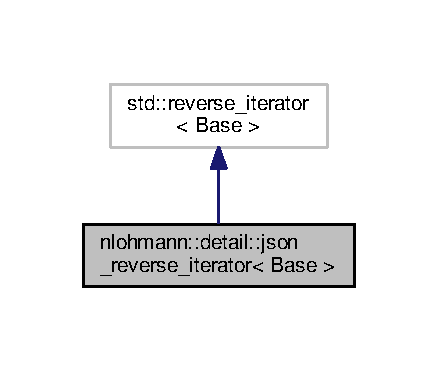
\includegraphics[width=210pt]{classnlohmann_1_1detail_1_1json__reverse__iterator__inherit__graph}
\end{center}
\end{figure}


Collaboration diagram for nlohmann\+:\+:detail\+:\+:json\+\_\+reverse\+\_\+iterator$<$ Base $>$\+:\nopagebreak
\begin{figure}[H]
\begin{center}
\leavevmode
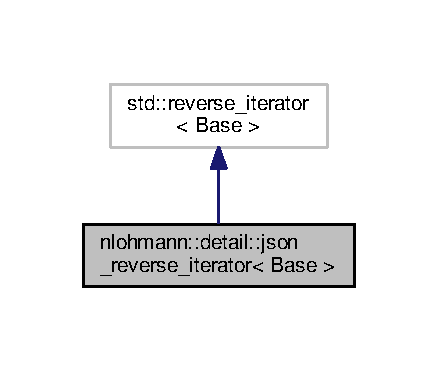
\includegraphics[width=210pt]{classnlohmann_1_1detail_1_1json__reverse__iterator__coll__graph}
\end{center}
\end{figure}
\subsection*{Public Types}
\begin{DoxyCompactItemize}
\item 
using \hyperlink{classnlohmann_1_1detail_1_1json__reverse__iterator_a9ab55987c05ec6427ad36082e351cc45}{difference\+\_\+type} = std\+::ptrdiff\+\_\+t
\item 
using \hyperlink{classnlohmann_1_1detail_1_1json__reverse__iterator_a6b2ef1d632fe49bfcc22fbd1abd62395}{base\+\_\+iterator} = std\+::reverse\+\_\+iterator$<$ Base $>$
\begin{DoxyCompactList}\small\item\em shortcut to the reverse iterator adaptor \end{DoxyCompactList}\item 
using \hyperlink{classnlohmann_1_1detail_1_1json__reverse__iterator_a42f51a69bac7b2aebb613b2164e457f1}{reference} = typename Base\+::reference
\begin{DoxyCompactList}\small\item\em the reference type for the pointed-\/to element \end{DoxyCompactList}\end{DoxyCompactItemize}
\subsection*{Public Member Functions}
\begin{DoxyCompactItemize}
\item 
\hyperlink{classnlohmann_1_1detail_1_1json__reverse__iterator_a0246de16ece16293f2917dfa5d96e278}{json\+\_\+reverse\+\_\+iterator} (const typename base\+\_\+iterator\+::iterator\+\_\+type \&it) noexcept
\begin{DoxyCompactList}\small\item\em create reverse iterator from iterator \end{DoxyCompactList}\item 
\hyperlink{classnlohmann_1_1detail_1_1json__reverse__iterator_a6c2d025530114ed989188e8adfc8467e}{json\+\_\+reverse\+\_\+iterator} (const \hyperlink{classnlohmann_1_1detail_1_1json__reverse__iterator_a6b2ef1d632fe49bfcc22fbd1abd62395}{base\+\_\+iterator} \&it) noexcept
\begin{DoxyCompactList}\small\item\em create reverse iterator from base class \end{DoxyCompactList}\item 
\hyperlink{classnlohmann_1_1detail_1_1json__reverse__iterator}{json\+\_\+reverse\+\_\+iterator} \hyperlink{classnlohmann_1_1detail_1_1json__reverse__iterator_a7ec568b1d3e0827569a5bf1628ceae02}{operator++} (int)
\begin{DoxyCompactList}\small\item\em post-\/increment (it++) \end{DoxyCompactList}\item 
\hyperlink{classnlohmann_1_1detail_1_1json__reverse__iterator}{json\+\_\+reverse\+\_\+iterator} \& \hyperlink{classnlohmann_1_1detail_1_1json__reverse__iterator_a26caf0069a50ce4ecb010a1453e883fc}{operator++} ()
\begin{DoxyCompactList}\small\item\em pre-\/increment (++it) \end{DoxyCompactList}\item 
\hyperlink{classnlohmann_1_1detail_1_1json__reverse__iterator}{json\+\_\+reverse\+\_\+iterator} \hyperlink{classnlohmann_1_1detail_1_1json__reverse__iterator_a6a3048605070171acba5f4cebaef0af8}{operator-\/-\/} (int)
\begin{DoxyCompactList}\small\item\em post-\/decrement (it--) \end{DoxyCompactList}\item 
\hyperlink{classnlohmann_1_1detail_1_1json__reverse__iterator}{json\+\_\+reverse\+\_\+iterator} \& \hyperlink{classnlohmann_1_1detail_1_1json__reverse__iterator_a2488d6a902103610943920ac49d12a04}{operator-\/-\/} ()
\begin{DoxyCompactList}\small\item\em pre-\/decrement (--it) \end{DoxyCompactList}\item 
\hyperlink{classnlohmann_1_1detail_1_1json__reverse__iterator}{json\+\_\+reverse\+\_\+iterator} \& \hyperlink{classnlohmann_1_1detail_1_1json__reverse__iterator_a4e5d0a3bee433104ef87366e00536e01}{operator+=} (\hyperlink{classnlohmann_1_1detail_1_1json__reverse__iterator_a9ab55987c05ec6427ad36082e351cc45}{difference\+\_\+type} i)
\begin{DoxyCompactList}\small\item\em add to iterator \end{DoxyCompactList}\item 
\hyperlink{classnlohmann_1_1detail_1_1json__reverse__iterator}{json\+\_\+reverse\+\_\+iterator} \hyperlink{classnlohmann_1_1detail_1_1json__reverse__iterator_a400e366bf323c7bffc1b279b00c73e93}{operator+} (\hyperlink{classnlohmann_1_1detail_1_1json__reverse__iterator_a9ab55987c05ec6427ad36082e351cc45}{difference\+\_\+type} i) const 
\begin{DoxyCompactList}\small\item\em add to iterator \end{DoxyCompactList}\item 
\hyperlink{classnlohmann_1_1detail_1_1json__reverse__iterator}{json\+\_\+reverse\+\_\+iterator} \hyperlink{classnlohmann_1_1detail_1_1json__reverse__iterator_a9c9404de5f78134575e5f0aead10676f}{operator-\/} (\hyperlink{classnlohmann_1_1detail_1_1json__reverse__iterator_a9ab55987c05ec6427ad36082e351cc45}{difference\+\_\+type} i) const 
\begin{DoxyCompactList}\small\item\em subtract from iterator \end{DoxyCompactList}\item 
\hyperlink{classnlohmann_1_1detail_1_1json__reverse__iterator_a9ab55987c05ec6427ad36082e351cc45}{difference\+\_\+type} \hyperlink{classnlohmann_1_1detail_1_1json__reverse__iterator_a2133803d87acc5bbb89f4c72adc43a0a}{operator-\/} (const \hyperlink{classnlohmann_1_1detail_1_1json__reverse__iterator}{json\+\_\+reverse\+\_\+iterator} \&other) const 
\begin{DoxyCompactList}\small\item\em return difference \end{DoxyCompactList}\item 
\hyperlink{classnlohmann_1_1detail_1_1json__reverse__iterator_a42f51a69bac7b2aebb613b2164e457f1}{reference} \hyperlink{classnlohmann_1_1detail_1_1json__reverse__iterator_ad01fd54e148e36d9e24cf9ad0fe31d00}{operator\mbox{[}$\,$\mbox{]}} (\hyperlink{classnlohmann_1_1detail_1_1json__reverse__iterator_a9ab55987c05ec6427ad36082e351cc45}{difference\+\_\+type} n) const 
\begin{DoxyCompactList}\small\item\em access to successor \end{DoxyCompactList}\item 
auto \hyperlink{classnlohmann_1_1detail_1_1json__reverse__iterator_adc648a641e8e9a1072c5abd56ad06401}{key} () const -\/$>$ decltype(std\+::declval$<$ Base $>$().key())
\begin{DoxyCompactList}\small\item\em return the key of an object iterator \end{DoxyCompactList}\item 
\hyperlink{classnlohmann_1_1detail_1_1json__reverse__iterator_a42f51a69bac7b2aebb613b2164e457f1}{reference} \hyperlink{classnlohmann_1_1detail_1_1json__reverse__iterator_a4c4e94317f95315f95e9909cf8d65dbf}{value} () const 
\begin{DoxyCompactList}\small\item\em return the value of an iterator \end{DoxyCompactList}\end{DoxyCompactItemize}


\subsection{Detailed Description}
\subsubsection*{template$<$typename Base$>$\\*
class nlohmann\+::detail\+::json\+\_\+reverse\+\_\+iterator$<$ Base $>$}

a template for a reverse iterator class 


\begin{DoxyTemplParams}{Template Parameters}
{\em Base} & the base iterator type to reverse. Valid types are iterator (to create reverse\+\_\+iterator) and const\+\_\+iterator (to create const\+\_\+reverse\+\_\+iterator).\\
\hline
\end{DoxyTemplParams}
The class satisfies the following concept requirements\+:
\begin{DoxyItemize}
\item \href{http://en.cppreference.com/w/cpp/concept/RandomAccessIterator}{\tt Random\+Access\+Iterator}\+: The iterator that can be moved to point (forward and backward) to any element in constant time.
\item \href{http://en.cppreference.com/w/cpp/concept/OutputIterator}{\tt Output\+Iterator}\+: It is possible to write to the pointed-\/to element (only if {\itshape Base} is iterator).
\end{DoxyItemize}

\begin{DoxySince}{Since}
version 1.\+0.\+0 
\end{DoxySince}


Definition at line 4261 of file json.\+hpp.



\subsection{Member Typedef Documentation}
\index{nlohmann\+::detail\+::json\+\_\+reverse\+\_\+iterator@{nlohmann\+::detail\+::json\+\_\+reverse\+\_\+iterator}!base\+\_\+iterator@{base\+\_\+iterator}}
\index{base\+\_\+iterator@{base\+\_\+iterator}!nlohmann\+::detail\+::json\+\_\+reverse\+\_\+iterator@{nlohmann\+::detail\+::json\+\_\+reverse\+\_\+iterator}}
\subsubsection[{\texorpdfstring{base\+\_\+iterator}{base_iterator}}]{\setlength{\rightskip}{0pt plus 5cm}template$<$typename Base $>$ using {\bf nlohmann\+::detail\+::json\+\_\+reverse\+\_\+iterator}$<$ Base $>$\+::{\bf base\+\_\+iterator} =  std\+::reverse\+\_\+iterator$<$Base$>$}\hypertarget{classnlohmann_1_1detail_1_1json__reverse__iterator_a6b2ef1d632fe49bfcc22fbd1abd62395}{}\label{classnlohmann_1_1detail_1_1json__reverse__iterator_a6b2ef1d632fe49bfcc22fbd1abd62395}


shortcut to the reverse iterator adaptor 



Definition at line 4266 of file json.\+hpp.

\index{nlohmann\+::detail\+::json\+\_\+reverse\+\_\+iterator@{nlohmann\+::detail\+::json\+\_\+reverse\+\_\+iterator}!difference\+\_\+type@{difference\+\_\+type}}
\index{difference\+\_\+type@{difference\+\_\+type}!nlohmann\+::detail\+::json\+\_\+reverse\+\_\+iterator@{nlohmann\+::detail\+::json\+\_\+reverse\+\_\+iterator}}
\subsubsection[{\texorpdfstring{difference\+\_\+type}{difference_type}}]{\setlength{\rightskip}{0pt plus 5cm}template$<$typename Base $>$ using {\bf nlohmann\+::detail\+::json\+\_\+reverse\+\_\+iterator}$<$ Base $>$\+::{\bf difference\+\_\+type} =  std\+::ptrdiff\+\_\+t}\hypertarget{classnlohmann_1_1detail_1_1json__reverse__iterator_a9ab55987c05ec6427ad36082e351cc45}{}\label{classnlohmann_1_1detail_1_1json__reverse__iterator_a9ab55987c05ec6427ad36082e351cc45}


Definition at line 4264 of file json.\+hpp.

\index{nlohmann\+::detail\+::json\+\_\+reverse\+\_\+iterator@{nlohmann\+::detail\+::json\+\_\+reverse\+\_\+iterator}!reference@{reference}}
\index{reference@{reference}!nlohmann\+::detail\+::json\+\_\+reverse\+\_\+iterator@{nlohmann\+::detail\+::json\+\_\+reverse\+\_\+iterator}}
\subsubsection[{\texorpdfstring{reference}{reference}}]{\setlength{\rightskip}{0pt plus 5cm}template$<$typename Base $>$ using {\bf nlohmann\+::detail\+::json\+\_\+reverse\+\_\+iterator}$<$ Base $>$\+::{\bf reference} =  typename Base\+::reference}\hypertarget{classnlohmann_1_1detail_1_1json__reverse__iterator_a42f51a69bac7b2aebb613b2164e457f1}{}\label{classnlohmann_1_1detail_1_1json__reverse__iterator_a42f51a69bac7b2aebb613b2164e457f1}


the reference type for the pointed-\/to element 



Definition at line 4268 of file json.\+hpp.



\subsection{Constructor \& Destructor Documentation}
\index{nlohmann\+::detail\+::json\+\_\+reverse\+\_\+iterator@{nlohmann\+::detail\+::json\+\_\+reverse\+\_\+iterator}!json\+\_\+reverse\+\_\+iterator@{json\+\_\+reverse\+\_\+iterator}}
\index{json\+\_\+reverse\+\_\+iterator@{json\+\_\+reverse\+\_\+iterator}!nlohmann\+::detail\+::json\+\_\+reverse\+\_\+iterator@{nlohmann\+::detail\+::json\+\_\+reverse\+\_\+iterator}}
\subsubsection[{\texorpdfstring{json\+\_\+reverse\+\_\+iterator(const typename base\+\_\+iterator\+::iterator\+\_\+type \&it) noexcept}{json_reverse_iterator(const typename base_iterator::iterator_type &it) noexcept}}]{\setlength{\rightskip}{0pt plus 5cm}template$<$typename Base $>$ {\bf nlohmann\+::detail\+::json\+\_\+reverse\+\_\+iterator}$<$ Base $>$\+::{\bf json\+\_\+reverse\+\_\+iterator} (
\begin{DoxyParamCaption}
\item[{const typename base\+\_\+iterator\+::iterator\+\_\+type \&}]{it}
\end{DoxyParamCaption}
)\hspace{0.3cm}{\ttfamily [inline]}, {\ttfamily [noexcept]}}\hypertarget{classnlohmann_1_1detail_1_1json__reverse__iterator_a0246de16ece16293f2917dfa5d96e278}{}\label{classnlohmann_1_1detail_1_1json__reverse__iterator_a0246de16ece16293f2917dfa5d96e278}


create reverse iterator from iterator 



Definition at line 4271 of file json.\+hpp.

\index{nlohmann\+::detail\+::json\+\_\+reverse\+\_\+iterator@{nlohmann\+::detail\+::json\+\_\+reverse\+\_\+iterator}!json\+\_\+reverse\+\_\+iterator@{json\+\_\+reverse\+\_\+iterator}}
\index{json\+\_\+reverse\+\_\+iterator@{json\+\_\+reverse\+\_\+iterator}!nlohmann\+::detail\+::json\+\_\+reverse\+\_\+iterator@{nlohmann\+::detail\+::json\+\_\+reverse\+\_\+iterator}}
\subsubsection[{\texorpdfstring{json\+\_\+reverse\+\_\+iterator(const base\+\_\+iterator \&it) noexcept}{json_reverse_iterator(const base_iterator &it) noexcept}}]{\setlength{\rightskip}{0pt plus 5cm}template$<$typename Base $>$ {\bf nlohmann\+::detail\+::json\+\_\+reverse\+\_\+iterator}$<$ Base $>$\+::{\bf json\+\_\+reverse\+\_\+iterator} (
\begin{DoxyParamCaption}
\item[{const {\bf base\+\_\+iterator} \&}]{it}
\end{DoxyParamCaption}
)\hspace{0.3cm}{\ttfamily [inline]}, {\ttfamily [noexcept]}}\hypertarget{classnlohmann_1_1detail_1_1json__reverse__iterator_a6c2d025530114ed989188e8adfc8467e}{}\label{classnlohmann_1_1detail_1_1json__reverse__iterator_a6c2d025530114ed989188e8adfc8467e}


create reverse iterator from base class 



Definition at line 4275 of file json.\+hpp.



\subsection{Member Function Documentation}
\index{nlohmann\+::detail\+::json\+\_\+reverse\+\_\+iterator@{nlohmann\+::detail\+::json\+\_\+reverse\+\_\+iterator}!key@{key}}
\index{key@{key}!nlohmann\+::detail\+::json\+\_\+reverse\+\_\+iterator@{nlohmann\+::detail\+::json\+\_\+reverse\+\_\+iterator}}
\subsubsection[{\texorpdfstring{key() const -\/$>$ decltype(std\+::declval$<$ Base $>$().\+key())}{key() const -> decltype(std::declval< Base >().key())}}]{\setlength{\rightskip}{0pt plus 5cm}template$<$typename Base $>$ auto {\bf nlohmann\+::detail\+::json\+\_\+reverse\+\_\+iterator}$<$ Base $>$\+::key (
\begin{DoxyParamCaption}
{}
\end{DoxyParamCaption}
) const -\/$>$ decltype(std\+::declval$<$Base$>$().key())
    \hspace{0.3cm}{\ttfamily [inline]}}\hypertarget{classnlohmann_1_1detail_1_1json__reverse__iterator_adc648a641e8e9a1072c5abd56ad06401}{}\label{classnlohmann_1_1detail_1_1json__reverse__iterator_adc648a641e8e9a1072c5abd56ad06401}


return the key of an object iterator 



Definition at line 4332 of file json.\+hpp.

\index{nlohmann\+::detail\+::json\+\_\+reverse\+\_\+iterator@{nlohmann\+::detail\+::json\+\_\+reverse\+\_\+iterator}!operator+@{operator+}}
\index{operator+@{operator+}!nlohmann\+::detail\+::json\+\_\+reverse\+\_\+iterator@{nlohmann\+::detail\+::json\+\_\+reverse\+\_\+iterator}}
\subsubsection[{\texorpdfstring{operator+(difference\+\_\+type i) const }{operator+(difference_type i) const }}]{\setlength{\rightskip}{0pt plus 5cm}template$<$typename Base $>$ {\bf json\+\_\+reverse\+\_\+iterator} {\bf nlohmann\+::detail\+::json\+\_\+reverse\+\_\+iterator}$<$ Base $>$\+::operator+ (
\begin{DoxyParamCaption}
\item[{{\bf difference\+\_\+type}}]{i}
\end{DoxyParamCaption}
) const\hspace{0.3cm}{\ttfamily [inline]}}\hypertarget{classnlohmann_1_1detail_1_1json__reverse__iterator_a400e366bf323c7bffc1b279b00c73e93}{}\label{classnlohmann_1_1detail_1_1json__reverse__iterator_a400e366bf323c7bffc1b279b00c73e93}


add to iterator 



Definition at line 4308 of file json.\+hpp.

\index{nlohmann\+::detail\+::json\+\_\+reverse\+\_\+iterator@{nlohmann\+::detail\+::json\+\_\+reverse\+\_\+iterator}!operator++@{operator++}}
\index{operator++@{operator++}!nlohmann\+::detail\+::json\+\_\+reverse\+\_\+iterator@{nlohmann\+::detail\+::json\+\_\+reverse\+\_\+iterator}}
\subsubsection[{\texorpdfstring{operator++(int)}{operator++(int)}}]{\setlength{\rightskip}{0pt plus 5cm}template$<$typename Base $>$ {\bf json\+\_\+reverse\+\_\+iterator} {\bf nlohmann\+::detail\+::json\+\_\+reverse\+\_\+iterator}$<$ Base $>$\+::operator++ (
\begin{DoxyParamCaption}
\item[{int}]{}
\end{DoxyParamCaption}
)\hspace{0.3cm}{\ttfamily [inline]}}\hypertarget{classnlohmann_1_1detail_1_1json__reverse__iterator_a7ec568b1d3e0827569a5bf1628ceae02}{}\label{classnlohmann_1_1detail_1_1json__reverse__iterator_a7ec568b1d3e0827569a5bf1628ceae02}


post-\/increment (it++) 



Definition at line 4278 of file json.\+hpp.

\index{nlohmann\+::detail\+::json\+\_\+reverse\+\_\+iterator@{nlohmann\+::detail\+::json\+\_\+reverse\+\_\+iterator}!operator++@{operator++}}
\index{operator++@{operator++}!nlohmann\+::detail\+::json\+\_\+reverse\+\_\+iterator@{nlohmann\+::detail\+::json\+\_\+reverse\+\_\+iterator}}
\subsubsection[{\texorpdfstring{operator++()}{operator++()}}]{\setlength{\rightskip}{0pt plus 5cm}template$<$typename Base $>$ {\bf json\+\_\+reverse\+\_\+iterator}\& {\bf nlohmann\+::detail\+::json\+\_\+reverse\+\_\+iterator}$<$ Base $>$\+::operator++ (
\begin{DoxyParamCaption}
{}
\end{DoxyParamCaption}
)\hspace{0.3cm}{\ttfamily [inline]}}\hypertarget{classnlohmann_1_1detail_1_1json__reverse__iterator_a26caf0069a50ce4ecb010a1453e883fc}{}\label{classnlohmann_1_1detail_1_1json__reverse__iterator_a26caf0069a50ce4ecb010a1453e883fc}


pre-\/increment (++it) 



Definition at line 4284 of file json.\+hpp.

\index{nlohmann\+::detail\+::json\+\_\+reverse\+\_\+iterator@{nlohmann\+::detail\+::json\+\_\+reverse\+\_\+iterator}!operator+=@{operator+=}}
\index{operator+=@{operator+=}!nlohmann\+::detail\+::json\+\_\+reverse\+\_\+iterator@{nlohmann\+::detail\+::json\+\_\+reverse\+\_\+iterator}}
\subsubsection[{\texorpdfstring{operator+=(difference\+\_\+type i)}{operator+=(difference_type i)}}]{\setlength{\rightskip}{0pt plus 5cm}template$<$typename Base $>$ {\bf json\+\_\+reverse\+\_\+iterator}\& {\bf nlohmann\+::detail\+::json\+\_\+reverse\+\_\+iterator}$<$ Base $>$\+::operator+= (
\begin{DoxyParamCaption}
\item[{{\bf difference\+\_\+type}}]{i}
\end{DoxyParamCaption}
)\hspace{0.3cm}{\ttfamily [inline]}}\hypertarget{classnlohmann_1_1detail_1_1json__reverse__iterator_a4e5d0a3bee433104ef87366e00536e01}{}\label{classnlohmann_1_1detail_1_1json__reverse__iterator_a4e5d0a3bee433104ef87366e00536e01}


add to iterator 



Definition at line 4302 of file json.\+hpp.

\index{nlohmann\+::detail\+::json\+\_\+reverse\+\_\+iterator@{nlohmann\+::detail\+::json\+\_\+reverse\+\_\+iterator}!operator-\/@{operator-\/}}
\index{operator-\/@{operator-\/}!nlohmann\+::detail\+::json\+\_\+reverse\+\_\+iterator@{nlohmann\+::detail\+::json\+\_\+reverse\+\_\+iterator}}
\subsubsection[{\texorpdfstring{operator-\/(difference\+\_\+type i) const }{operator-(difference_type i) const }}]{\setlength{\rightskip}{0pt plus 5cm}template$<$typename Base $>$ {\bf json\+\_\+reverse\+\_\+iterator} {\bf nlohmann\+::detail\+::json\+\_\+reverse\+\_\+iterator}$<$ Base $>$\+::operator-\/ (
\begin{DoxyParamCaption}
\item[{{\bf difference\+\_\+type}}]{i}
\end{DoxyParamCaption}
) const\hspace{0.3cm}{\ttfamily [inline]}}\hypertarget{classnlohmann_1_1detail_1_1json__reverse__iterator_a9c9404de5f78134575e5f0aead10676f}{}\label{classnlohmann_1_1detail_1_1json__reverse__iterator_a9c9404de5f78134575e5f0aead10676f}


subtract from iterator 



Definition at line 4314 of file json.\+hpp.

\index{nlohmann\+::detail\+::json\+\_\+reverse\+\_\+iterator@{nlohmann\+::detail\+::json\+\_\+reverse\+\_\+iterator}!operator-\/@{operator-\/}}
\index{operator-\/@{operator-\/}!nlohmann\+::detail\+::json\+\_\+reverse\+\_\+iterator@{nlohmann\+::detail\+::json\+\_\+reverse\+\_\+iterator}}
\subsubsection[{\texorpdfstring{operator-\/(const json\+\_\+reverse\+\_\+iterator \&other) const }{operator-(const json_reverse_iterator &other) const }}]{\setlength{\rightskip}{0pt plus 5cm}template$<$typename Base $>$ {\bf difference\+\_\+type} {\bf nlohmann\+::detail\+::json\+\_\+reverse\+\_\+iterator}$<$ Base $>$\+::operator-\/ (
\begin{DoxyParamCaption}
\item[{const {\bf json\+\_\+reverse\+\_\+iterator}$<$ Base $>$ \&}]{other}
\end{DoxyParamCaption}
) const\hspace{0.3cm}{\ttfamily [inline]}}\hypertarget{classnlohmann_1_1detail_1_1json__reverse__iterator_a2133803d87acc5bbb89f4c72adc43a0a}{}\label{classnlohmann_1_1detail_1_1json__reverse__iterator_a2133803d87acc5bbb89f4c72adc43a0a}


return difference 



Definition at line 4320 of file json.\+hpp.

\index{nlohmann\+::detail\+::json\+\_\+reverse\+\_\+iterator@{nlohmann\+::detail\+::json\+\_\+reverse\+\_\+iterator}!operator-\/-\/@{operator-\/-\/}}
\index{operator-\/-\/@{operator-\/-\/}!nlohmann\+::detail\+::json\+\_\+reverse\+\_\+iterator@{nlohmann\+::detail\+::json\+\_\+reverse\+\_\+iterator}}
\subsubsection[{\texorpdfstring{operator-\/-\/(int)}{operator--(int)}}]{\setlength{\rightskip}{0pt plus 5cm}template$<$typename Base $>$ {\bf json\+\_\+reverse\+\_\+iterator} {\bf nlohmann\+::detail\+::json\+\_\+reverse\+\_\+iterator}$<$ Base $>$\+::operator-\/-\/ (
\begin{DoxyParamCaption}
\item[{int}]{}
\end{DoxyParamCaption}
)\hspace{0.3cm}{\ttfamily [inline]}}\hypertarget{classnlohmann_1_1detail_1_1json__reverse__iterator_a6a3048605070171acba5f4cebaef0af8}{}\label{classnlohmann_1_1detail_1_1json__reverse__iterator_a6a3048605070171acba5f4cebaef0af8}


post-\/decrement (it--) 



Definition at line 4290 of file json.\+hpp.

\index{nlohmann\+::detail\+::json\+\_\+reverse\+\_\+iterator@{nlohmann\+::detail\+::json\+\_\+reverse\+\_\+iterator}!operator-\/-\/@{operator-\/-\/}}
\index{operator-\/-\/@{operator-\/-\/}!nlohmann\+::detail\+::json\+\_\+reverse\+\_\+iterator@{nlohmann\+::detail\+::json\+\_\+reverse\+\_\+iterator}}
\subsubsection[{\texorpdfstring{operator-\/-\/()}{operator--()}}]{\setlength{\rightskip}{0pt plus 5cm}template$<$typename Base $>$ {\bf json\+\_\+reverse\+\_\+iterator}\& {\bf nlohmann\+::detail\+::json\+\_\+reverse\+\_\+iterator}$<$ Base $>$\+::operator-\/-\/ (
\begin{DoxyParamCaption}
{}
\end{DoxyParamCaption}
)\hspace{0.3cm}{\ttfamily [inline]}}\hypertarget{classnlohmann_1_1detail_1_1json__reverse__iterator_a2488d6a902103610943920ac49d12a04}{}\label{classnlohmann_1_1detail_1_1json__reverse__iterator_a2488d6a902103610943920ac49d12a04}


pre-\/decrement (--it) 



Definition at line 4296 of file json.\+hpp.

\index{nlohmann\+::detail\+::json\+\_\+reverse\+\_\+iterator@{nlohmann\+::detail\+::json\+\_\+reverse\+\_\+iterator}!operator\mbox{[}$\,$\mbox{]}@{operator[]}}
\index{operator\mbox{[}$\,$\mbox{]}@{operator[]}!nlohmann\+::detail\+::json\+\_\+reverse\+\_\+iterator@{nlohmann\+::detail\+::json\+\_\+reverse\+\_\+iterator}}
\subsubsection[{\texorpdfstring{operator[](difference\+\_\+type n) const }{operator[](difference_type n) const }}]{\setlength{\rightskip}{0pt plus 5cm}template$<$typename Base $>$ {\bf reference} {\bf nlohmann\+::detail\+::json\+\_\+reverse\+\_\+iterator}$<$ Base $>$\+::operator\mbox{[}$\,$\mbox{]} (
\begin{DoxyParamCaption}
\item[{{\bf difference\+\_\+type}}]{n}
\end{DoxyParamCaption}
) const\hspace{0.3cm}{\ttfamily [inline]}}\hypertarget{classnlohmann_1_1detail_1_1json__reverse__iterator_ad01fd54e148e36d9e24cf9ad0fe31d00}{}\label{classnlohmann_1_1detail_1_1json__reverse__iterator_ad01fd54e148e36d9e24cf9ad0fe31d00}


access to successor 



Definition at line 4326 of file json.\+hpp.

\index{nlohmann\+::detail\+::json\+\_\+reverse\+\_\+iterator@{nlohmann\+::detail\+::json\+\_\+reverse\+\_\+iterator}!value@{value}}
\index{value@{value}!nlohmann\+::detail\+::json\+\_\+reverse\+\_\+iterator@{nlohmann\+::detail\+::json\+\_\+reverse\+\_\+iterator}}
\subsubsection[{\texorpdfstring{value() const }{value() const }}]{\setlength{\rightskip}{0pt plus 5cm}template$<$typename Base $>$ {\bf reference} {\bf nlohmann\+::detail\+::json\+\_\+reverse\+\_\+iterator}$<$ Base $>$\+::value (
\begin{DoxyParamCaption}
{}
\end{DoxyParamCaption}
) const\hspace{0.3cm}{\ttfamily [inline]}}\hypertarget{classnlohmann_1_1detail_1_1json__reverse__iterator_a4c4e94317f95315f95e9909cf8d65dbf}{}\label{classnlohmann_1_1detail_1_1json__reverse__iterator_a4c4e94317f95315f95e9909cf8d65dbf}


return the value of an iterator 



Definition at line 4339 of file json.\+hpp.



The documentation for this class was generated from the following file\+:\begin{DoxyCompactItemize}
\item 
include/\hyperlink{json_8hpp}{json.\+hpp}\end{DoxyCompactItemize}

\hypertarget{class_legacy_parser}{}\section{Legacy\+Parser Class Reference}
\label{class_legacy_parser}\index{Legacy\+Parser@{Legacy\+Parser}}


{\ttfamily \#include $<$parser.\+hpp$>$}

\subsection*{Public Member Functions}
\begin{DoxyCompactItemize}
\item 
\hyperlink{parser_8hpp_a76d816dc60daad0ab1c3c7b1dc7906d2}{phys\+\_\+quant} \hyperlink{class_legacy_parser_ae54110d322a9037b86e0b51e7038e06d}{get\+Quantity} (std\+::string input)
\begin{DoxyCompactList}\small\item\em Get number as value and vector of pairs of strings. \end{DoxyCompactList}\end{DoxyCompactItemize}


\subsection{Detailed Description}
D\+E\+P\+R\+E\+C\+A\+T\+ED -\/ Simple class to call boost\+::spirit parser to convert string to value and units. Kept because of neat parser template. 

Definition at line 72 of file parser.\+hpp.



\subsection{Member Function Documentation}
\index{Legacy\+Parser@{Legacy\+Parser}!get\+Quantity@{get\+Quantity}}
\index{get\+Quantity@{get\+Quantity}!Legacy\+Parser@{Legacy\+Parser}}
\subsubsection[{\texorpdfstring{get\+Quantity(std\+::string input)}{getQuantity(std::string input)}}]{\setlength{\rightskip}{0pt plus 5cm}{\bf phys\+\_\+quant} Legacy\+Parser\+::get\+Quantity (
\begin{DoxyParamCaption}
\item[{std\+::string}]{input}
\end{DoxyParamCaption}
)}\hypertarget{class_legacy_parser_ae54110d322a9037b86e0b51e7038e06d}{}\label{class_legacy_parser_ae54110d322a9037b86e0b51e7038e06d}


Get number as value and vector of pairs of strings. 


\begin{DoxyParams}{Parameters}
{\em input} & -\/ String of value and units. \\
\hline
\end{DoxyParams}
\begin{DoxyReturn}{Returns}
phys\+\_\+quant type containing value and units. 
\end{DoxyReturn}


Definition at line 105 of file Parser.\+cpp.



The documentation for this class was generated from the following files\+:\begin{DoxyCompactItemize}
\item 
include/\hyperlink{parser_8hpp}{parser.\+hpp}\item 
src/\hyperlink{_parser_8cpp}{Parser.\+cpp}\end{DoxyCompactItemize}

\hypertarget{structstd_1_1less_3_1_1nlohmann_1_1detail_1_1value__t_01_4}{}\section{std\+:\+:less$<$\+:\+:nlohmann\+:\+:detail\+:\+:value\+\_\+t $>$ Struct Template Reference}
\label{structstd_1_1less_3_1_1nlohmann_1_1detail_1_1value__t_01_4}\index{std\+::less$<$\+::nlohmann\+::detail\+::value\+\_\+t $>$@{std\+::less$<$\+::nlohmann\+::detail\+::value\+\_\+t $>$}}


specialization for std\+::less$<$value\+\_\+t$>$  




{\ttfamily \#include $<$json.\+hpp$>$}

\subsection*{Public Member Functions}
\begin{DoxyCompactItemize}
\item 
bool \hyperlink{structstd_1_1less_3_1_1nlohmann_1_1detail_1_1value__t_01_4_a10d3fea50edf7b15ead8f4ceeb006000}{operator()} (\hyperlink{namespacenlohmann_1_1detail_a90aa5ef615aa8305e9ea20d8a947980f}{nlohmann\+::detail\+::value\+\_\+t} lhs, \hyperlink{namespacenlohmann_1_1detail_a90aa5ef615aa8305e9ea20d8a947980f}{nlohmann\+::detail\+::value\+\_\+t} rhs) const noexcept
\begin{DoxyCompactList}\small\item\em compare two value\+\_\+t enum values \end{DoxyCompactList}\end{DoxyCompactItemize}


\subsection{Detailed Description}
\subsubsection*{template$<$$>$\\*
struct std\+::less$<$\+::nlohmann\+::detail\+::value\+\_\+t $>$}

specialization for std\+::less$<$value\+\_\+t$>$ 

Definition at line 14495 of file json.\+hpp.



\subsection{Member Function Documentation}
\index{std\+::less$<$\+::nlohmann\+::detail\+::value\+\_\+t $>$@{std\+::less$<$\+::nlohmann\+::detail\+::value\+\_\+t $>$}!operator()@{operator()}}
\index{operator()@{operator()}!std\+::less$<$\+::nlohmann\+::detail\+::value\+\_\+t $>$@{std\+::less$<$\+::nlohmann\+::detail\+::value\+\_\+t $>$}}
\subsubsection[{\texorpdfstring{operator()(nlohmann\+::detail\+::value\+\_\+t lhs, nlohmann\+::detail\+::value\+\_\+t rhs) const noexcept}{operator()(nlohmann::detail::value_t lhs, nlohmann::detail::value_t rhs) const noexcept}}]{\setlength{\rightskip}{0pt plus 5cm}bool std\+::less$<$\+::{\bf nlohmann\+::detail\+::value\+\_\+t} $>$\+::operator() (
\begin{DoxyParamCaption}
\item[{{\bf nlohmann\+::detail\+::value\+\_\+t}}]{lhs, }
\item[{{\bf nlohmann\+::detail\+::value\+\_\+t}}]{rhs}
\end{DoxyParamCaption}
) const\hspace{0.3cm}{\ttfamily [inline]}, {\ttfamily [noexcept]}}\hypertarget{structstd_1_1less_3_1_1nlohmann_1_1detail_1_1value__t_01_4_a10d3fea50edf7b15ead8f4ceeb006000}{}\label{structstd_1_1less_3_1_1nlohmann_1_1detail_1_1value__t_01_4_a10d3fea50edf7b15ead8f4ceeb006000}


compare two value\+\_\+t enum values 

\begin{DoxySince}{Since}
version 3.\+0.\+0 
\end{DoxySince}


Definition at line 14501 of file json.\+hpp.



The documentation for this struct was generated from the following file\+:\begin{DoxyCompactItemize}
\item 
include/\hyperlink{json_8hpp}{json.\+hpp}\end{DoxyCompactItemize}

\hypertarget{classnlohmann_1_1detail_1_1lexer}{}\section{nlohmann\+:\+:detail\+:\+:lexer$<$ Basic\+Json\+Type $>$ Class Template Reference}
\label{classnlohmann_1_1detail_1_1lexer}\index{nlohmann\+::detail\+::lexer$<$ Basic\+Json\+Type $>$@{nlohmann\+::detail\+::lexer$<$ Basic\+Json\+Type $>$}}


lexical analysis  




{\ttfamily \#include $<$json.\+hpp$>$}

\subsection*{Public Types}
\begin{DoxyCompactItemize}
\item 
enum \hyperlink{classnlohmann_1_1detail_1_1lexer_a3f313cdbe187cababfc5e06f0b69b098}{token\+\_\+type} \{ \\*
\hyperlink{classnlohmann_1_1detail_1_1lexer_a3f313cdbe187cababfc5e06f0b69b098a42dd1a73d072bb6bf3f494f22b15db8e}{token\+\_\+type\+::uninitialized}, 
\hyperlink{classnlohmann_1_1detail_1_1lexer_a3f313cdbe187cababfc5e06f0b69b098a85cc1a37b0aaa52de40e72f0ed4e0c0d}{token\+\_\+type\+::literal\+\_\+true}, 
\hyperlink{classnlohmann_1_1detail_1_1lexer_a3f313cdbe187cababfc5e06f0b69b098afab1694b1b3937a079f4625fe0b6108b}{token\+\_\+type\+::literal\+\_\+false}, 
\hyperlink{classnlohmann_1_1detail_1_1lexer_a3f313cdbe187cababfc5e06f0b69b098ab7ae4c0e46d86f884677768160b26e9e}{token\+\_\+type\+::literal\+\_\+null}, 
\\*
\hyperlink{classnlohmann_1_1detail_1_1lexer_a3f313cdbe187cababfc5e06f0b69b098a2b490e8bf366b4cbe3ebd99b26ce15ce}{token\+\_\+type\+::value\+\_\+string}, 
\hyperlink{classnlohmann_1_1detail_1_1lexer_a3f313cdbe187cababfc5e06f0b69b098aaf1f040fcd2f674d2e5893d7a731078f}{token\+\_\+type\+::value\+\_\+unsigned}, 
\hyperlink{classnlohmann_1_1detail_1_1lexer_a3f313cdbe187cababfc5e06f0b69b098a5064b6655d88a50ae16665cf7751c0ee}{token\+\_\+type\+::value\+\_\+integer}, 
\hyperlink{classnlohmann_1_1detail_1_1lexer_a3f313cdbe187cababfc5e06f0b69b098a0d2671a6f81efb91e77f6ac3bdb11443}{token\+\_\+type\+::value\+\_\+float}, 
\\*
\hyperlink{classnlohmann_1_1detail_1_1lexer_a3f313cdbe187cababfc5e06f0b69b098a16c226b4425b68560fea322b46dabe01}{token\+\_\+type\+::begin\+\_\+array}, 
\hyperlink{classnlohmann_1_1detail_1_1lexer_a3f313cdbe187cababfc5e06f0b69b098a9a9ffd53b6869d4eca271b1ed5b57fe8}{token\+\_\+type\+::begin\+\_\+object}, 
\hyperlink{classnlohmann_1_1detail_1_1lexer_a3f313cdbe187cababfc5e06f0b69b098a2f3e68e7f111a1e5c7728742b3ca2b7f}{token\+\_\+type\+::end\+\_\+array}, 
\hyperlink{classnlohmann_1_1detail_1_1lexer_a3f313cdbe187cababfc5e06f0b69b098a7d5b4427866814de4d8f132721d59c87}{token\+\_\+type\+::end\+\_\+object}, 
\\*
\hyperlink{classnlohmann_1_1detail_1_1lexer_a3f313cdbe187cababfc5e06f0b69b098acc3c64f8ae08c00de1b33f19a4d2913a}{token\+\_\+type\+::name\+\_\+separator}, 
\hyperlink{classnlohmann_1_1detail_1_1lexer_a3f313cdbe187cababfc5e06f0b69b098a745373036100d7392ad62c617cab59af}{token\+\_\+type\+::value\+\_\+separator}, 
\hyperlink{classnlohmann_1_1detail_1_1lexer_a3f313cdbe187cababfc5e06f0b69b098a456e19aeafa334241c7ff3f589547f9d}{token\+\_\+type\+::parse\+\_\+error}, 
\hyperlink{classnlohmann_1_1detail_1_1lexer_a3f313cdbe187cababfc5e06f0b69b098aca11f56dd477c09e06583dbdcda0985f}{token\+\_\+type\+::end\+\_\+of\+\_\+input}, 
\\*
\hyperlink{classnlohmann_1_1detail_1_1lexer_a3f313cdbe187cababfc5e06f0b69b098ad2a8e6f6721cccec0b466301dd9495a5}{token\+\_\+type\+::literal\+\_\+or\+\_\+value}
 \}\begin{DoxyCompactList}\small\item\em token types for the parser \end{DoxyCompactList}
\end{DoxyCompactItemize}
\subsection*{Public Member Functions}
\begin{DoxyCompactItemize}
\item 
\hyperlink{classnlohmann_1_1detail_1_1lexer_a0d7de7b99bc839ea9a39dd738d05d89c}{lexer} (\hyperlink{namespacenlohmann_1_1detail_ae132f8cd5bb24c5e9b40ad0eafedf1c2}{detail\+::input\+\_\+adapter\+\_\+t} adapter)
\item 
\hyperlink{classnlohmann_1_1detail_1_1lexer_a2e8ce2a0d266d148b69dfbcc2e4ad71a}{lexer} (const \hyperlink{classnlohmann_1_1detail_1_1lexer}{lexer} \&)=delete
\item 
\hyperlink{classnlohmann_1_1detail_1_1lexer}{lexer} \& \hyperlink{classnlohmann_1_1detail_1_1lexer_a33e97dee7c5faf1b36aff5b74a6c8f55}{operator=} (\hyperlink{classnlohmann_1_1detail_1_1lexer}{lexer} \&)=delete
\item 
constexpr number\+\_\+integer\+\_\+t \hyperlink{classnlohmann_1_1detail_1_1lexer_afa338d17c0a7e834c73104258a2c8ced}{get\+\_\+number\+\_\+integer} () const noexcept
\begin{DoxyCompactList}\small\item\em return integer value \end{DoxyCompactList}\item 
constexpr number\+\_\+unsigned\+\_\+t \hyperlink{classnlohmann_1_1detail_1_1lexer_a56640fb92293e0c17742ca3c814d74d6}{get\+\_\+number\+\_\+unsigned} () const noexcept
\begin{DoxyCompactList}\small\item\em return unsigned integer value \end{DoxyCompactList}\item 
constexpr number\+\_\+float\+\_\+t \hyperlink{classnlohmann_1_1detail_1_1lexer_ac013af35a21e9387993b19da5b3e0ae2}{get\+\_\+number\+\_\+float} () const noexcept
\begin{DoxyCompactList}\small\item\em return floating-\/point value \end{DoxyCompactList}\item 
const \hyperlink{namespacenlohmann_1_1detail_a90aa5ef615aa8305e9ea20d8a947980fab45cffe084dd3d20d928bee85e7b0f21}{std\+::string} \hyperlink{classnlohmann_1_1detail_1_1lexer_a61e3bf22aa79c402f26670560b6198b0}{get\+\_\+string} ()
\begin{DoxyCompactList}\small\item\em return string value \end{DoxyCompactList}\item 
constexpr std\+::size\+\_\+t \hyperlink{classnlohmann_1_1detail_1_1lexer_a2a00465a3d5d70c84809cdb27658db79}{get\+\_\+position} () const noexcept
\begin{DoxyCompactList}\small\item\em return position of last read token \end{DoxyCompactList}\item 
\hyperlink{namespacenlohmann_1_1detail_a90aa5ef615aa8305e9ea20d8a947980fab45cffe084dd3d20d928bee85e7b0f21}{std\+::string} \hyperlink{classnlohmann_1_1detail_1_1lexer_a6d8a58be845717a86726756372414cbb}{get\+\_\+token\+\_\+string} () const 
\begin{DoxyCompactList}\small\item\em return the last read token (for errors only) \end{DoxyCompactList}\item 
constexpr const char $\ast$ \hyperlink{classnlohmann_1_1detail_1_1lexer_a53cebbc684ef97fa49651eb442d58f86}{get\+\_\+error\+\_\+message} () const noexcept
\begin{DoxyCompactList}\small\item\em return syntax error message \end{DoxyCompactList}\item 
\hyperlink{classnlohmann_1_1detail_1_1lexer_a3f313cdbe187cababfc5e06f0b69b098}{token\+\_\+type} \hyperlink{classnlohmann_1_1detail_1_1lexer_aac3041cd2b9291e64fee38db422863c9}{scan} ()
\end{DoxyCompactItemize}
\subsection*{Static Public Member Functions}
\begin{DoxyCompactItemize}
\item 
static const char $\ast$ \hyperlink{classnlohmann_1_1detail_1_1lexer_ae514e2005f0ce185f1ad366139e541e8}{token\+\_\+type\+\_\+name} (const \hyperlink{classnlohmann_1_1detail_1_1lexer_a3f313cdbe187cababfc5e06f0b69b098}{token\+\_\+type} t) noexcept
\begin{DoxyCompactList}\small\item\em return name of values of type token\+\_\+type (only used for errors) \end{DoxyCompactList}\end{DoxyCompactItemize}


\subsection{Detailed Description}
\subsubsection*{template$<$typename Basic\+Json\+Type$>$\\*
class nlohmann\+::detail\+::lexer$<$ Basic\+Json\+Type $>$}

lexical analysis 

This class organizes the lexical analysis during J\+S\+ON deserialization. 

Definition at line 1566 of file json.\+hpp.



\subsection{Member Enumeration Documentation}
\index{nlohmann\+::detail\+::lexer@{nlohmann\+::detail\+::lexer}!token\+\_\+type@{token\+\_\+type}}
\index{token\+\_\+type@{token\+\_\+type}!nlohmann\+::detail\+::lexer@{nlohmann\+::detail\+::lexer}}
\subsubsection[{\texorpdfstring{token\+\_\+type}{token_type}}]{\setlength{\rightskip}{0pt plus 5cm}template$<$typename Basic\+Json\+Type $>$ enum {\bf nlohmann\+::detail\+::lexer\+::token\+\_\+type}\hspace{0.3cm}{\ttfamily [strong]}}\hypertarget{classnlohmann_1_1detail_1_1lexer_a3f313cdbe187cababfc5e06f0b69b098}{}\label{classnlohmann_1_1detail_1_1lexer_a3f313cdbe187cababfc5e06f0b69b098}


token types for the parser 

\begin{Desc}
\item[Enumerator]\par
\begin{description}
\index{uninitialized@{uninitialized}!nlohmann\+::detail\+::lexer@{nlohmann\+::detail\+::lexer}}\index{nlohmann\+::detail\+::lexer@{nlohmann\+::detail\+::lexer}!uninitialized@{uninitialized}}\item[{\em 
uninitialized\hypertarget{classnlohmann_1_1detail_1_1lexer_a3f313cdbe187cababfc5e06f0b69b098a42dd1a73d072bb6bf3f494f22b15db8e}{}\label{classnlohmann_1_1detail_1_1lexer_a3f313cdbe187cababfc5e06f0b69b098a42dd1a73d072bb6bf3f494f22b15db8e}
}]indicating the scanner is uninitialized \index{literal\+\_\+true@{literal\+\_\+true}!nlohmann\+::detail\+::lexer@{nlohmann\+::detail\+::lexer}}\index{nlohmann\+::detail\+::lexer@{nlohmann\+::detail\+::lexer}!literal\+\_\+true@{literal\+\_\+true}}\item[{\em 
literal\+\_\+true\hypertarget{classnlohmann_1_1detail_1_1lexer_a3f313cdbe187cababfc5e06f0b69b098a85cc1a37b0aaa52de40e72f0ed4e0c0d}{}\label{classnlohmann_1_1detail_1_1lexer_a3f313cdbe187cababfc5e06f0b69b098a85cc1a37b0aaa52de40e72f0ed4e0c0d}
}]the {\ttfamily true} literal \index{literal\+\_\+false@{literal\+\_\+false}!nlohmann\+::detail\+::lexer@{nlohmann\+::detail\+::lexer}}\index{nlohmann\+::detail\+::lexer@{nlohmann\+::detail\+::lexer}!literal\+\_\+false@{literal\+\_\+false}}\item[{\em 
literal\+\_\+false\hypertarget{classnlohmann_1_1detail_1_1lexer_a3f313cdbe187cababfc5e06f0b69b098afab1694b1b3937a079f4625fe0b6108b}{}\label{classnlohmann_1_1detail_1_1lexer_a3f313cdbe187cababfc5e06f0b69b098afab1694b1b3937a079f4625fe0b6108b}
}]the {\ttfamily false} literal \index{literal\+\_\+null@{literal\+\_\+null}!nlohmann\+::detail\+::lexer@{nlohmann\+::detail\+::lexer}}\index{nlohmann\+::detail\+::lexer@{nlohmann\+::detail\+::lexer}!literal\+\_\+null@{literal\+\_\+null}}\item[{\em 
literal\+\_\+null\hypertarget{classnlohmann_1_1detail_1_1lexer_a3f313cdbe187cababfc5e06f0b69b098ab7ae4c0e46d86f884677768160b26e9e}{}\label{classnlohmann_1_1detail_1_1lexer_a3f313cdbe187cababfc5e06f0b69b098ab7ae4c0e46d86f884677768160b26e9e}
}]the {\ttfamily null} literal \index{value\+\_\+string@{value\+\_\+string}!nlohmann\+::detail\+::lexer@{nlohmann\+::detail\+::lexer}}\index{nlohmann\+::detail\+::lexer@{nlohmann\+::detail\+::lexer}!value\+\_\+string@{value\+\_\+string}}\item[{\em 
value\+\_\+string\hypertarget{classnlohmann_1_1detail_1_1lexer_a3f313cdbe187cababfc5e06f0b69b098a2b490e8bf366b4cbe3ebd99b26ce15ce}{}\label{classnlohmann_1_1detail_1_1lexer_a3f313cdbe187cababfc5e06f0b69b098a2b490e8bf366b4cbe3ebd99b26ce15ce}
}]a string -- use \hyperlink{classnlohmann_1_1detail_1_1lexer_a61e3bf22aa79c402f26670560b6198b0}{get\+\_\+string()} for actual value \index{value\+\_\+unsigned@{value\+\_\+unsigned}!nlohmann\+::detail\+::lexer@{nlohmann\+::detail\+::lexer}}\index{nlohmann\+::detail\+::lexer@{nlohmann\+::detail\+::lexer}!value\+\_\+unsigned@{value\+\_\+unsigned}}\item[{\em 
value\+\_\+unsigned\hypertarget{classnlohmann_1_1detail_1_1lexer_a3f313cdbe187cababfc5e06f0b69b098aaf1f040fcd2f674d2e5893d7a731078f}{}\label{classnlohmann_1_1detail_1_1lexer_a3f313cdbe187cababfc5e06f0b69b098aaf1f040fcd2f674d2e5893d7a731078f}
}]an unsigned integer -- use \hyperlink{classnlohmann_1_1detail_1_1lexer_a56640fb92293e0c17742ca3c814d74d6}{get\+\_\+number\+\_\+unsigned()} for actual value \index{value\+\_\+integer@{value\+\_\+integer}!nlohmann\+::detail\+::lexer@{nlohmann\+::detail\+::lexer}}\index{nlohmann\+::detail\+::lexer@{nlohmann\+::detail\+::lexer}!value\+\_\+integer@{value\+\_\+integer}}\item[{\em 
value\+\_\+integer\hypertarget{classnlohmann_1_1detail_1_1lexer_a3f313cdbe187cababfc5e06f0b69b098a5064b6655d88a50ae16665cf7751c0ee}{}\label{classnlohmann_1_1detail_1_1lexer_a3f313cdbe187cababfc5e06f0b69b098a5064b6655d88a50ae16665cf7751c0ee}
}]a signed integer -- use \hyperlink{classnlohmann_1_1detail_1_1lexer_afa338d17c0a7e834c73104258a2c8ced}{get\+\_\+number\+\_\+integer()} for actual value \index{value\+\_\+float@{value\+\_\+float}!nlohmann\+::detail\+::lexer@{nlohmann\+::detail\+::lexer}}\index{nlohmann\+::detail\+::lexer@{nlohmann\+::detail\+::lexer}!value\+\_\+float@{value\+\_\+float}}\item[{\em 
value\+\_\+float\hypertarget{classnlohmann_1_1detail_1_1lexer_a3f313cdbe187cababfc5e06f0b69b098a0d2671a6f81efb91e77f6ac3bdb11443}{}\label{classnlohmann_1_1detail_1_1lexer_a3f313cdbe187cababfc5e06f0b69b098a0d2671a6f81efb91e77f6ac3bdb11443}
}]an floating point number -- use \hyperlink{classnlohmann_1_1detail_1_1lexer_ac013af35a21e9387993b19da5b3e0ae2}{get\+\_\+number\+\_\+float()} for actual value \index{begin\+\_\+array@{begin\+\_\+array}!nlohmann\+::detail\+::lexer@{nlohmann\+::detail\+::lexer}}\index{nlohmann\+::detail\+::lexer@{nlohmann\+::detail\+::lexer}!begin\+\_\+array@{begin\+\_\+array}}\item[{\em 
begin\+\_\+array\hypertarget{classnlohmann_1_1detail_1_1lexer_a3f313cdbe187cababfc5e06f0b69b098a16c226b4425b68560fea322b46dabe01}{}\label{classnlohmann_1_1detail_1_1lexer_a3f313cdbe187cababfc5e06f0b69b098a16c226b4425b68560fea322b46dabe01}
}]the character for array begin {\ttfamily \mbox{[}} \index{begin\+\_\+object@{begin\+\_\+object}!nlohmann\+::detail\+::lexer@{nlohmann\+::detail\+::lexer}}\index{nlohmann\+::detail\+::lexer@{nlohmann\+::detail\+::lexer}!begin\+\_\+object@{begin\+\_\+object}}\item[{\em 
begin\+\_\+object\hypertarget{classnlohmann_1_1detail_1_1lexer_a3f313cdbe187cababfc5e06f0b69b098a9a9ffd53b6869d4eca271b1ed5b57fe8}{}\label{classnlohmann_1_1detail_1_1lexer_a3f313cdbe187cababfc5e06f0b69b098a9a9ffd53b6869d4eca271b1ed5b57fe8}
}]the character for object begin {\ttfamily \{} \index{end\+\_\+array@{end\+\_\+array}!nlohmann\+::detail\+::lexer@{nlohmann\+::detail\+::lexer}}\index{nlohmann\+::detail\+::lexer@{nlohmann\+::detail\+::lexer}!end\+\_\+array@{end\+\_\+array}}\item[{\em 
end\+\_\+array\hypertarget{classnlohmann_1_1detail_1_1lexer_a3f313cdbe187cababfc5e06f0b69b098a2f3e68e7f111a1e5c7728742b3ca2b7f}{}\label{classnlohmann_1_1detail_1_1lexer_a3f313cdbe187cababfc5e06f0b69b098a2f3e68e7f111a1e5c7728742b3ca2b7f}
}]the character for array end {\ttfamily \mbox{]}} \index{end\+\_\+object@{end\+\_\+object}!nlohmann\+::detail\+::lexer@{nlohmann\+::detail\+::lexer}}\index{nlohmann\+::detail\+::lexer@{nlohmann\+::detail\+::lexer}!end\+\_\+object@{end\+\_\+object}}\item[{\em 
end\+\_\+object\hypertarget{classnlohmann_1_1detail_1_1lexer_a3f313cdbe187cababfc5e06f0b69b098a7d5b4427866814de4d8f132721d59c87}{}\label{classnlohmann_1_1detail_1_1lexer_a3f313cdbe187cababfc5e06f0b69b098a7d5b4427866814de4d8f132721d59c87}
}]the character for object end {\ttfamily \}} \index{name\+\_\+separator@{name\+\_\+separator}!nlohmann\+::detail\+::lexer@{nlohmann\+::detail\+::lexer}}\index{nlohmann\+::detail\+::lexer@{nlohmann\+::detail\+::lexer}!name\+\_\+separator@{name\+\_\+separator}}\item[{\em 
name\+\_\+separator\hypertarget{classnlohmann_1_1detail_1_1lexer_a3f313cdbe187cababfc5e06f0b69b098acc3c64f8ae08c00de1b33f19a4d2913a}{}\label{classnlohmann_1_1detail_1_1lexer_a3f313cdbe187cababfc5e06f0b69b098acc3c64f8ae08c00de1b33f19a4d2913a}
}]the name separator {\ttfamily \+:} \index{value\+\_\+separator@{value\+\_\+separator}!nlohmann\+::detail\+::lexer@{nlohmann\+::detail\+::lexer}}\index{nlohmann\+::detail\+::lexer@{nlohmann\+::detail\+::lexer}!value\+\_\+separator@{value\+\_\+separator}}\item[{\em 
value\+\_\+separator\hypertarget{classnlohmann_1_1detail_1_1lexer_a3f313cdbe187cababfc5e06f0b69b098a745373036100d7392ad62c617cab59af}{}\label{classnlohmann_1_1detail_1_1lexer_a3f313cdbe187cababfc5e06f0b69b098a745373036100d7392ad62c617cab59af}
}]the value separator {\ttfamily ,} \index{parse\+\_\+error@{parse\+\_\+error}!nlohmann\+::detail\+::lexer@{nlohmann\+::detail\+::lexer}}\index{nlohmann\+::detail\+::lexer@{nlohmann\+::detail\+::lexer}!parse\+\_\+error@{parse\+\_\+error}}\item[{\em 
parse\+\_\+error\hypertarget{classnlohmann_1_1detail_1_1lexer_a3f313cdbe187cababfc5e06f0b69b098a456e19aeafa334241c7ff3f589547f9d}{}\label{classnlohmann_1_1detail_1_1lexer_a3f313cdbe187cababfc5e06f0b69b098a456e19aeafa334241c7ff3f589547f9d}
}]indicating a parse error \index{end\+\_\+of\+\_\+input@{end\+\_\+of\+\_\+input}!nlohmann\+::detail\+::lexer@{nlohmann\+::detail\+::lexer}}\index{nlohmann\+::detail\+::lexer@{nlohmann\+::detail\+::lexer}!end\+\_\+of\+\_\+input@{end\+\_\+of\+\_\+input}}\item[{\em 
end\+\_\+of\+\_\+input\hypertarget{classnlohmann_1_1detail_1_1lexer_a3f313cdbe187cababfc5e06f0b69b098aca11f56dd477c09e06583dbdcda0985f}{}\label{classnlohmann_1_1detail_1_1lexer_a3f313cdbe187cababfc5e06f0b69b098aca11f56dd477c09e06583dbdcda0985f}
}]indicating the end of the input buffer \index{literal\+\_\+or\+\_\+value@{literal\+\_\+or\+\_\+value}!nlohmann\+::detail\+::lexer@{nlohmann\+::detail\+::lexer}}\index{nlohmann\+::detail\+::lexer@{nlohmann\+::detail\+::lexer}!literal\+\_\+or\+\_\+value@{literal\+\_\+or\+\_\+value}}\item[{\em 
literal\+\_\+or\+\_\+value\hypertarget{classnlohmann_1_1detail_1_1lexer_a3f313cdbe187cababfc5e06f0b69b098ad2a8e6f6721cccec0b466301dd9495a5}{}\label{classnlohmann_1_1detail_1_1lexer_a3f313cdbe187cababfc5e06f0b69b098ad2a8e6f6721cccec0b466301dd9495a5}
}]a literal or the begin of a value (only for diagnostics) \end{description}
\end{Desc}


Definition at line 1574 of file json.\+hpp.



\subsection{Constructor \& Destructor Documentation}
\index{nlohmann\+::detail\+::lexer@{nlohmann\+::detail\+::lexer}!lexer@{lexer}}
\index{lexer@{lexer}!nlohmann\+::detail\+::lexer@{nlohmann\+::detail\+::lexer}}
\subsubsection[{\texorpdfstring{lexer(detail\+::input\+\_\+adapter\+\_\+t adapter)}{lexer(detail::input_adapter_t adapter)}}]{\setlength{\rightskip}{0pt plus 5cm}template$<$typename Basic\+Json\+Type $>$ {\bf nlohmann\+::detail\+::lexer}$<$ Basic\+Json\+Type $>$\+::{\bf lexer} (
\begin{DoxyParamCaption}
\item[{{\bf detail\+::input\+\_\+adapter\+\_\+t}}]{adapter}
\end{DoxyParamCaption}
)\hspace{0.3cm}{\ttfamily [inline]}, {\ttfamily [explicit]}}\hypertarget{classnlohmann_1_1detail_1_1lexer_a0d7de7b99bc839ea9a39dd738d05d89c}{}\label{classnlohmann_1_1detail_1_1lexer_a0d7de7b99bc839ea9a39dd738d05d89c}


Definition at line 1640 of file json.\+hpp.

\index{nlohmann\+::detail\+::lexer@{nlohmann\+::detail\+::lexer}!lexer@{lexer}}
\index{lexer@{lexer}!nlohmann\+::detail\+::lexer@{nlohmann\+::detail\+::lexer}}
\subsubsection[{\texorpdfstring{lexer(const lexer \&)=delete}{lexer(const lexer &)=delete}}]{\setlength{\rightskip}{0pt plus 5cm}template$<$typename Basic\+Json\+Type $>$ {\bf nlohmann\+::detail\+::lexer}$<$ Basic\+Json\+Type $>$\+::{\bf lexer} (
\begin{DoxyParamCaption}
\item[{const {\bf lexer}$<$ Basic\+Json\+Type $>$ \&}]{}
\end{DoxyParamCaption}
)\hspace{0.3cm}{\ttfamily [delete]}}\hypertarget{classnlohmann_1_1detail_1_1lexer_a2e8ce2a0d266d148b69dfbcc2e4ad71a}{}\label{classnlohmann_1_1detail_1_1lexer_a2e8ce2a0d266d148b69dfbcc2e4ad71a}


\subsection{Member Function Documentation}
\index{nlohmann\+::detail\+::lexer@{nlohmann\+::detail\+::lexer}!get\+\_\+error\+\_\+message@{get\+\_\+error\+\_\+message}}
\index{get\+\_\+error\+\_\+message@{get\+\_\+error\+\_\+message}!nlohmann\+::detail\+::lexer@{nlohmann\+::detail\+::lexer}}
\subsubsection[{\texorpdfstring{get\+\_\+error\+\_\+message() const noexcept}{get_error_message() const noexcept}}]{\setlength{\rightskip}{0pt plus 5cm}template$<$typename Basic\+Json\+Type $>$ constexpr const char$\ast$ {\bf nlohmann\+::detail\+::lexer}$<$ Basic\+Json\+Type $>$\+::get\+\_\+error\+\_\+message (
\begin{DoxyParamCaption}
{}
\end{DoxyParamCaption}
) const\hspace{0.3cm}{\ttfamily [inline]}, {\ttfamily [noexcept]}}\hypertarget{classnlohmann_1_1detail_1_1lexer_a53cebbc684ef97fa49651eb442d58f86}{}\label{classnlohmann_1_1detail_1_1lexer_a53cebbc684ef97fa49651eb442d58f86}


return syntax error message 



Definition at line 2711 of file json.\+hpp.

\index{nlohmann\+::detail\+::lexer@{nlohmann\+::detail\+::lexer}!get\+\_\+number\+\_\+float@{get\+\_\+number\+\_\+float}}
\index{get\+\_\+number\+\_\+float@{get\+\_\+number\+\_\+float}!nlohmann\+::detail\+::lexer@{nlohmann\+::detail\+::lexer}}
\subsubsection[{\texorpdfstring{get\+\_\+number\+\_\+float() const noexcept}{get_number_float() const noexcept}}]{\setlength{\rightskip}{0pt plus 5cm}template$<$typename Basic\+Json\+Type $>$ constexpr number\+\_\+float\+\_\+t {\bf nlohmann\+::detail\+::lexer}$<$ Basic\+Json\+Type $>$\+::get\+\_\+number\+\_\+float (
\begin{DoxyParamCaption}
{}
\end{DoxyParamCaption}
) const\hspace{0.3cm}{\ttfamily [inline]}, {\ttfamily [noexcept]}}\hypertarget{classnlohmann_1_1detail_1_1lexer_ac013af35a21e9387993b19da5b3e0ae2}{}\label{classnlohmann_1_1detail_1_1lexer_ac013af35a21e9387993b19da5b3e0ae2}


return floating-\/point value 



Definition at line 2654 of file json.\+hpp.

\index{nlohmann\+::detail\+::lexer@{nlohmann\+::detail\+::lexer}!get\+\_\+number\+\_\+integer@{get\+\_\+number\+\_\+integer}}
\index{get\+\_\+number\+\_\+integer@{get\+\_\+number\+\_\+integer}!nlohmann\+::detail\+::lexer@{nlohmann\+::detail\+::lexer}}
\subsubsection[{\texorpdfstring{get\+\_\+number\+\_\+integer() const noexcept}{get_number_integer() const noexcept}}]{\setlength{\rightskip}{0pt plus 5cm}template$<$typename Basic\+Json\+Type $>$ constexpr number\+\_\+integer\+\_\+t {\bf nlohmann\+::detail\+::lexer}$<$ Basic\+Json\+Type $>$\+::get\+\_\+number\+\_\+integer (
\begin{DoxyParamCaption}
{}
\end{DoxyParamCaption}
) const\hspace{0.3cm}{\ttfamily [inline]}, {\ttfamily [noexcept]}}\hypertarget{classnlohmann_1_1detail_1_1lexer_afa338d17c0a7e834c73104258a2c8ced}{}\label{classnlohmann_1_1detail_1_1lexer_afa338d17c0a7e834c73104258a2c8ced}


return integer value 



Definition at line 2642 of file json.\+hpp.

\index{nlohmann\+::detail\+::lexer@{nlohmann\+::detail\+::lexer}!get\+\_\+number\+\_\+unsigned@{get\+\_\+number\+\_\+unsigned}}
\index{get\+\_\+number\+\_\+unsigned@{get\+\_\+number\+\_\+unsigned}!nlohmann\+::detail\+::lexer@{nlohmann\+::detail\+::lexer}}
\subsubsection[{\texorpdfstring{get\+\_\+number\+\_\+unsigned() const noexcept}{get_number_unsigned() const noexcept}}]{\setlength{\rightskip}{0pt plus 5cm}template$<$typename Basic\+Json\+Type $>$ constexpr number\+\_\+unsigned\+\_\+t {\bf nlohmann\+::detail\+::lexer}$<$ Basic\+Json\+Type $>$\+::get\+\_\+number\+\_\+unsigned (
\begin{DoxyParamCaption}
{}
\end{DoxyParamCaption}
) const\hspace{0.3cm}{\ttfamily [inline]}, {\ttfamily [noexcept]}}\hypertarget{classnlohmann_1_1detail_1_1lexer_a56640fb92293e0c17742ca3c814d74d6}{}\label{classnlohmann_1_1detail_1_1lexer_a56640fb92293e0c17742ca3c814d74d6}


return unsigned integer value 



Definition at line 2648 of file json.\+hpp.

\index{nlohmann\+::detail\+::lexer@{nlohmann\+::detail\+::lexer}!get\+\_\+position@{get\+\_\+position}}
\index{get\+\_\+position@{get\+\_\+position}!nlohmann\+::detail\+::lexer@{nlohmann\+::detail\+::lexer}}
\subsubsection[{\texorpdfstring{get\+\_\+position() const noexcept}{get_position() const noexcept}}]{\setlength{\rightskip}{0pt plus 5cm}template$<$typename Basic\+Json\+Type $>$ constexpr std\+::size\+\_\+t {\bf nlohmann\+::detail\+::lexer}$<$ Basic\+Json\+Type $>$\+::get\+\_\+position (
\begin{DoxyParamCaption}
{}
\end{DoxyParamCaption}
) const\hspace{0.3cm}{\ttfamily [inline]}, {\ttfamily [noexcept]}}\hypertarget{classnlohmann_1_1detail_1_1lexer_a2a00465a3d5d70c84809cdb27658db79}{}\label{classnlohmann_1_1detail_1_1lexer_a2a00465a3d5d70c84809cdb27658db79}


return position of last read token 



Definition at line 2672 of file json.\+hpp.

\index{nlohmann\+::detail\+::lexer@{nlohmann\+::detail\+::lexer}!get\+\_\+string@{get\+\_\+string}}
\index{get\+\_\+string@{get\+\_\+string}!nlohmann\+::detail\+::lexer@{nlohmann\+::detail\+::lexer}}
\subsubsection[{\texorpdfstring{get\+\_\+string()}{get_string()}}]{\setlength{\rightskip}{0pt plus 5cm}template$<$typename Basic\+Json\+Type $>$ const {\bf std\+::string} {\bf nlohmann\+::detail\+::lexer}$<$ Basic\+Json\+Type $>$\+::get\+\_\+string (
\begin{DoxyParamCaption}
{}
\end{DoxyParamCaption}
)\hspace{0.3cm}{\ttfamily [inline]}}\hypertarget{classnlohmann_1_1detail_1_1lexer_a61e3bf22aa79c402f26670560b6198b0}{}\label{classnlohmann_1_1detail_1_1lexer_a61e3bf22aa79c402f26670560b6198b0}


return string value 



Definition at line 2660 of file json.\+hpp.

\index{nlohmann\+::detail\+::lexer@{nlohmann\+::detail\+::lexer}!get\+\_\+token\+\_\+string@{get\+\_\+token\+\_\+string}}
\index{get\+\_\+token\+\_\+string@{get\+\_\+token\+\_\+string}!nlohmann\+::detail\+::lexer@{nlohmann\+::detail\+::lexer}}
\subsubsection[{\texorpdfstring{get\+\_\+token\+\_\+string() const }{get_token_string() const }}]{\setlength{\rightskip}{0pt plus 5cm}template$<$typename Basic\+Json\+Type $>$ {\bf std\+::string} {\bf nlohmann\+::detail\+::lexer}$<$ Basic\+Json\+Type $>$\+::get\+\_\+token\+\_\+string (
\begin{DoxyParamCaption}
{}
\end{DoxyParamCaption}
) const\hspace{0.3cm}{\ttfamily [inline]}}\hypertarget{classnlohmann_1_1detail_1_1lexer_a6d8a58be845717a86726756372414cbb}{}\label{classnlohmann_1_1detail_1_1lexer_a6d8a58be845717a86726756372414cbb}


return the last read token (for errors only) 



Definition at line 2678 of file json.\+hpp.

\index{nlohmann\+::detail\+::lexer@{nlohmann\+::detail\+::lexer}!operator=@{operator=}}
\index{operator=@{operator=}!nlohmann\+::detail\+::lexer@{nlohmann\+::detail\+::lexer}}
\subsubsection[{\texorpdfstring{operator=(lexer \&)=delete}{operator=(lexer &)=delete}}]{\setlength{\rightskip}{0pt plus 5cm}template$<$typename Basic\+Json\+Type $>$ {\bf lexer}\& {\bf nlohmann\+::detail\+::lexer}$<$ Basic\+Json\+Type $>$\+::operator= (
\begin{DoxyParamCaption}
\item[{{\bf lexer}$<$ Basic\+Json\+Type $>$ \&}]{}
\end{DoxyParamCaption}
)\hspace{0.3cm}{\ttfamily [delete]}}\hypertarget{classnlohmann_1_1detail_1_1lexer_a33e97dee7c5faf1b36aff5b74a6c8f55}{}\label{classnlohmann_1_1detail_1_1lexer_a33e97dee7c5faf1b36aff5b74a6c8f55}
\index{nlohmann\+::detail\+::lexer@{nlohmann\+::detail\+::lexer}!scan@{scan}}
\index{scan@{scan}!nlohmann\+::detail\+::lexer@{nlohmann\+::detail\+::lexer}}
\subsubsection[{\texorpdfstring{scan()}{scan()}}]{\setlength{\rightskip}{0pt plus 5cm}template$<$typename Basic\+Json\+Type $>$ {\bf token\+\_\+type} {\bf nlohmann\+::detail\+::lexer}$<$ Basic\+Json\+Type $>$\+::scan (
\begin{DoxyParamCaption}
{}
\end{DoxyParamCaption}
)\hspace{0.3cm}{\ttfamily [inline]}}\hypertarget{classnlohmann_1_1detail_1_1lexer_aac3041cd2b9291e64fee38db422863c9}{}\label{classnlohmann_1_1detail_1_1lexer_aac3041cd2b9291e64fee38db422863c9}


Definition at line 2720 of file json.\+hpp.

\index{nlohmann\+::detail\+::lexer@{nlohmann\+::detail\+::lexer}!token\+\_\+type\+\_\+name@{token\+\_\+type\+\_\+name}}
\index{token\+\_\+type\+\_\+name@{token\+\_\+type\+\_\+name}!nlohmann\+::detail\+::lexer@{nlohmann\+::detail\+::lexer}}
\subsubsection[{\texorpdfstring{token\+\_\+type\+\_\+name(const token\+\_\+type t) noexcept}{token_type_name(const token_type t) noexcept}}]{\setlength{\rightskip}{0pt plus 5cm}template$<$typename Basic\+Json\+Type $>$ static const char$\ast$ {\bf nlohmann\+::detail\+::lexer}$<$ Basic\+Json\+Type $>$\+::token\+\_\+type\+\_\+name (
\begin{DoxyParamCaption}
\item[{const {\bf token\+\_\+type}}]{t}
\end{DoxyParamCaption}
)\hspace{0.3cm}{\ttfamily [inline]}, {\ttfamily [static]}, {\ttfamily [noexcept]}}\hypertarget{classnlohmann_1_1detail_1_1lexer_ae514e2005f0ce185f1ad366139e541e8}{}\label{classnlohmann_1_1detail_1_1lexer_ae514e2005f0ce185f1ad366139e541e8}


return name of values of type token\+\_\+type (only used for errors) 



Definition at line 1596 of file json.\+hpp.



The documentation for this class was generated from the following file\+:\begin{DoxyCompactItemize}
\item 
include/\hyperlink{json_8hpp}{json.\+hpp}\end{DoxyCompactItemize}

\hypertarget{structnlohmann_1_1detail_1_1make__index__sequence}{}\section{nlohmann\+:\+:detail\+:\+:make\+\_\+index\+\_\+sequence$<$ N $>$ Struct Template Reference}
\label{structnlohmann_1_1detail_1_1make__index__sequence}\index{nlohmann\+::detail\+::make\+\_\+index\+\_\+sequence$<$ N $>$@{nlohmann\+::detail\+::make\+\_\+index\+\_\+sequence$<$ N $>$}}


{\ttfamily \#include $<$json.\+hpp$>$}



Inheritance diagram for nlohmann\+:\+:detail\+:\+:make\+\_\+index\+\_\+sequence$<$ N $>$\+:\nopagebreak
\begin{figure}[H]
\begin{center}
\leavevmode
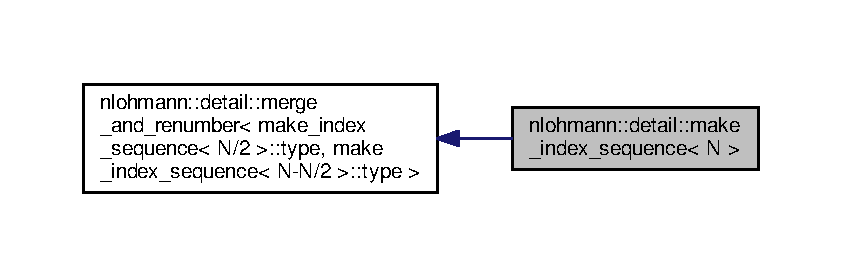
\includegraphics[width=350pt]{structnlohmann_1_1detail_1_1make__index__sequence__inherit__graph}
\end{center}
\end{figure}


Collaboration diagram for nlohmann\+:\+:detail\+:\+:make\+\_\+index\+\_\+sequence$<$ N $>$\+:\nopagebreak
\begin{figure}[H]
\begin{center}
\leavevmode
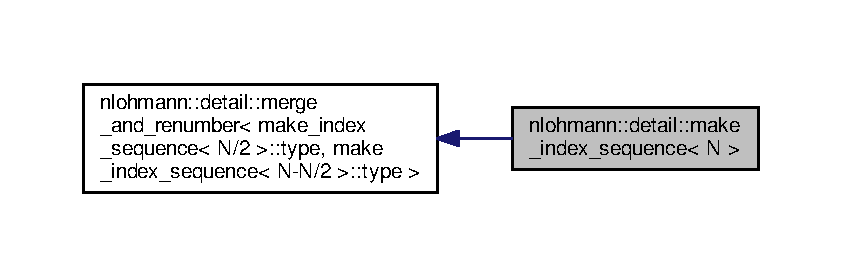
\includegraphics[width=350pt]{structnlohmann_1_1detail_1_1make__index__sequence__coll__graph}
\end{center}
\end{figure}


\subsection{Detailed Description}
\subsubsection*{template$<$std\+::size\+\_\+t N$>$\\*
struct nlohmann\+::detail\+::make\+\_\+index\+\_\+sequence$<$ N $>$}



Definition at line 514 of file json.\+hpp.



The documentation for this struct was generated from the following file\+:\begin{DoxyCompactItemize}
\item 
include/\hyperlink{json_8hpp}{json.\+hpp}\end{DoxyCompactItemize}

\hypertarget{structnlohmann_1_1detail_1_1make__index__sequence_3_010_01_4}{}\section{nlohmann\+:\+:detail\+:\+:make\+\_\+index\+\_\+sequence$<$ 0 $>$ Struct Template Reference}
\label{structnlohmann_1_1detail_1_1make__index__sequence_3_010_01_4}\index{nlohmann\+::detail\+::make\+\_\+index\+\_\+sequence$<$ 0 $>$@{nlohmann\+::detail\+::make\+\_\+index\+\_\+sequence$<$ 0 $>$}}


{\ttfamily \#include $<$json.\+hpp$>$}



Inheritance diagram for nlohmann\+:\+:detail\+:\+:make\+\_\+index\+\_\+sequence$<$ 0 $>$\+:\nopagebreak
\begin{figure}[H]
\begin{center}
\leavevmode
\includegraphics[width=198pt]{structnlohmann_1_1detail_1_1make__index__sequence_3_010_01_4__inherit__graph}
\end{center}
\end{figure}


Collaboration diagram for nlohmann\+:\+:detail\+:\+:make\+\_\+index\+\_\+sequence$<$ 0 $>$\+:\nopagebreak
\begin{figure}[H]
\begin{center}
\leavevmode
\includegraphics[width=198pt]{structnlohmann_1_1detail_1_1make__index__sequence_3_010_01_4__coll__graph}
\end{center}
\end{figure}
\subsection*{Additional Inherited Members}


\subsection{Detailed Description}
\subsubsection*{template$<$$>$\\*
struct nlohmann\+::detail\+::make\+\_\+index\+\_\+sequence$<$ 0 $>$}



Definition at line 519 of file json.\+hpp.



The documentation for this struct was generated from the following file\+:\begin{DoxyCompactItemize}
\item 
include/\hyperlink{json_8hpp}{json.\+hpp}\end{DoxyCompactItemize}

\hypertarget{structnlohmann_1_1detail_1_1make__index__sequence_3_011_01_4}{}\section{nlohmann\+:\+:detail\+:\+:make\+\_\+index\+\_\+sequence$<$ 1 $>$ Struct Template Reference}
\label{structnlohmann_1_1detail_1_1make__index__sequence_3_011_01_4}\index{nlohmann\+::detail\+::make\+\_\+index\+\_\+sequence$<$ 1 $>$@{nlohmann\+::detail\+::make\+\_\+index\+\_\+sequence$<$ 1 $>$}}


{\ttfamily \#include $<$json.\+hpp$>$}



Inheritance diagram for nlohmann\+:\+:detail\+:\+:make\+\_\+index\+\_\+sequence$<$ 1 $>$\+:\nopagebreak
\begin{figure}[H]
\begin{center}
\leavevmode
\includegraphics[width=198pt]{structnlohmann_1_1detail_1_1make__index__sequence_3_011_01_4__inherit__graph}
\end{center}
\end{figure}


Collaboration diagram for nlohmann\+:\+:detail\+:\+:make\+\_\+index\+\_\+sequence$<$ 1 $>$\+:\nopagebreak
\begin{figure}[H]
\begin{center}
\leavevmode
\includegraphics[width=198pt]{structnlohmann_1_1detail_1_1make__index__sequence_3_011_01_4__coll__graph}
\end{center}
\end{figure}
\subsection*{Additional Inherited Members}


\subsection{Detailed Description}
\subsubsection*{template$<$$>$\\*
struct nlohmann\+::detail\+::make\+\_\+index\+\_\+sequence$<$ 1 $>$}



Definition at line 520 of file json.\+hpp.



The documentation for this struct was generated from the following file\+:\begin{DoxyCompactItemize}
\item 
include/\hyperlink{json_8hpp}{json.\+hpp}\end{DoxyCompactItemize}

\hypertarget{structnlohmann_1_1detail_1_1merge__and__renumber}{}\section{nlohmann\+:\+:detail\+:\+:merge\+\_\+and\+\_\+renumber$<$ Sequence1, Sequence2 $>$ Struct Template Reference}
\label{structnlohmann_1_1detail_1_1merge__and__renumber}\index{nlohmann\+::detail\+::merge\+\_\+and\+\_\+renumber$<$ Sequence1, Sequence2 $>$@{nlohmann\+::detail\+::merge\+\_\+and\+\_\+renumber$<$ Sequence1, Sequence2 $>$}}


{\ttfamily \#include $<$json.\+hpp$>$}



\subsection{Detailed Description}
\subsubsection*{template$<$class Sequence1, class Sequence2$>$\\*
struct nlohmann\+::detail\+::merge\+\_\+and\+\_\+renumber$<$ Sequence1, Sequence2 $>$}



Definition at line 506 of file json.\+hpp.



The documentation for this struct was generated from the following file\+:\begin{DoxyCompactItemize}
\item 
include/\hyperlink{json_8hpp}{json.\+hpp}\end{DoxyCompactItemize}

\hypertarget{structnlohmann_1_1detail_1_1merge__and__renumber_3_01index__sequence_3_01_i1_8_8_8_01_4_00_01indf5ec8c9c7b5107e4b381e3ca4c1be2ca}{}\section{nlohmann\+:\+:detail\+:\+:merge\+\_\+and\+\_\+renumber$<$ index\+\_\+sequence$<$ I1... $>$, index\+\_\+sequence$<$ I2... $>$ $>$ Struct Template Reference}
\label{structnlohmann_1_1detail_1_1merge__and__renumber_3_01index__sequence_3_01_i1_8_8_8_01_4_00_01indf5ec8c9c7b5107e4b381e3ca4c1be2ca}\index{nlohmann\+::detail\+::merge\+\_\+and\+\_\+renumber$<$ index\+\_\+sequence$<$ I1... $>$, index\+\_\+sequence$<$ I2... $>$ $>$@{nlohmann\+::detail\+::merge\+\_\+and\+\_\+renumber$<$ index\+\_\+sequence$<$ I1... $>$, index\+\_\+sequence$<$ I2... $>$ $>$}}


{\ttfamily \#include $<$json.\+hpp$>$}



Inheritance diagram for nlohmann\+:\+:detail\+:\+:merge\+\_\+and\+\_\+renumber$<$ index\+\_\+sequence$<$ I1... $>$, index\+\_\+sequence$<$ I2... $>$ $>$\+:\nopagebreak
\begin{figure}[H]
\begin{center}
\leavevmode
\includegraphics[width=243pt]{structnlohmann_1_1detail_1_1merge__and__renumber_3_01index__sequence_3_01_i1_8_8_8_01_4_00_01ind6c27662b24eb9b5dea448f2c0400428a}
\end{center}
\end{figure}


Collaboration diagram for nlohmann\+:\+:detail\+:\+:merge\+\_\+and\+\_\+renumber$<$ index\+\_\+sequence$<$ I1... $>$, index\+\_\+sequence$<$ I2... $>$ $>$\+:\nopagebreak
\begin{figure}[H]
\begin{center}
\leavevmode
\includegraphics[width=243pt]{structnlohmann_1_1detail_1_1merge__and__renumber_3_01index__sequence_3_01_i1_8_8_8_01_4_00_01ind7f3f7d0d4c10bc1f158de4a327478fcd}
\end{center}
\end{figure}
\subsection*{Additional Inherited Members}


\subsection{Detailed Description}
\subsubsection*{template$<$std\+::size\+\_\+t... I1, std\+::size\+\_\+t... I2$>$\\*
struct nlohmann\+::detail\+::merge\+\_\+and\+\_\+renumber$<$ index\+\_\+sequence$<$ I1... $>$, index\+\_\+sequence$<$ I2... $>$ $>$}



Definition at line 509 of file json.\+hpp.



The documentation for this struct was generated from the following file\+:\begin{DoxyCompactItemize}
\item 
include/\hyperlink{json_8hpp}{json.\+hpp}\end{DoxyCompactItemize}

\hypertarget{structnlohmann_1_1detail_1_1negation}{}\section{nlohmann\+:\+:detail\+:\+:negation$<$ B $>$ Struct Template Reference}
\label{structnlohmann_1_1detail_1_1negation}\index{nlohmann\+::detail\+::negation$<$ B $>$@{nlohmann\+::detail\+::negation$<$ B $>$}}


{\ttfamily \#include $<$json.\+hpp$>$}



Inheritance diagram for nlohmann\+:\+:detail\+:\+:negation$<$ B $>$\+:\nopagebreak
\begin{figure}[H]
\begin{center}
\leavevmode
\includegraphics[width=235pt]{structnlohmann_1_1detail_1_1negation__inherit__graph}
\end{center}
\end{figure}


Collaboration diagram for nlohmann\+:\+:detail\+:\+:negation$<$ B $>$\+:\nopagebreak
\begin{figure}[H]
\begin{center}
\leavevmode
\includegraphics[width=235pt]{structnlohmann_1_1detail_1_1negation__coll__graph}
\end{center}
\end{figure}


\subsection{Detailed Description}
\subsubsection*{template$<$class B$>$\\*
struct nlohmann\+::detail\+::negation$<$ B $>$}



Definition at line 543 of file json.\+hpp.



The documentation for this struct was generated from the following file\+:\begin{DoxyCompactItemize}
\item 
include/\hyperlink{json_8hpp}{json.\+hpp}\end{DoxyCompactItemize}

\hypertarget{classnlohmann_1_1detail_1_1other__error}{}\section{nlohmann\+:\+:detail\+:\+:other\+\_\+error Class Reference}
\label{classnlohmann_1_1detail_1_1other__error}\index{nlohmann\+::detail\+::other\+\_\+error@{nlohmann\+::detail\+::other\+\_\+error}}


exception indicating other errors  




{\ttfamily \#include $<$json.\+hpp$>$}



Inheritance diagram for nlohmann\+:\+:detail\+:\+:other\+\_\+error\+:\nopagebreak
\begin{figure}[H]
\begin{center}
\leavevmode
\includegraphics[width=216pt]{classnlohmann_1_1detail_1_1other__error__inherit__graph}
\end{center}
\end{figure}


Collaboration diagram for nlohmann\+:\+:detail\+:\+:other\+\_\+error\+:\nopagebreak
\begin{figure}[H]
\begin{center}
\leavevmode
\includegraphics[width=216pt]{classnlohmann_1_1detail_1_1other__error__coll__graph}
\end{center}
\end{figure}
\subsection*{Static Public Member Functions}
\begin{DoxyCompactItemize}
\item 
static \hyperlink{classnlohmann_1_1detail_1_1other__error}{other\+\_\+error} \hyperlink{classnlohmann_1_1detail_1_1other__error_a1443f7682e7dd05144a577f0d3765c63}{create} (int \hyperlink{classnlohmann_1_1detail_1_1exception_a0d4589a3fb54e81646d986c05efa3b9a}{id}, const \hyperlink{namespacenlohmann_1_1detail_a90aa5ef615aa8305e9ea20d8a947980fab45cffe084dd3d20d928bee85e7b0f21}{std\+::string} \&what\+\_\+arg)
\end{DoxyCompactItemize}
\subsection*{Additional Inherited Members}


\subsection{Detailed Description}
exception indicating other errors 

Exceptions have ids 5xx.

\tabulinesep=1mm
\begin{longtabu} spread 0pt [c]{*3{|X[-1]}|}
\hline
\rowcolor{\tableheadbgcolor}{\bf name / id }&{\bf example message }&{\bf description  }\\\cline{1-3}
\endfirsthead
\hline
\endfoot
\hline
\rowcolor{\tableheadbgcolor}{\bf name / id }&{\bf example message }&{\bf description  }\\\cline{1-3}
\endhead
json.\+exception.\+other\+\_\+error.\+501 &unsuccessful\+: \{\char`\"{}op\char`\"{}\+:\char`\"{}test\char`\"{},\char`\"{}path\char`\"{}\+:\char`\"{}/baz\char`\"{}, \char`\"{}value\char`\"{}\+:\char`\"{}bar\char`\"{}\} &A J\+S\+ON Patch operation \textquotesingle{}test\textquotesingle{} failed. The unsuccessful operation is also printed. \\\cline{1-3}
json.\+exception.\+other\+\_\+error.\+502 &invalid object size for conversion &Some conversions to user-\/defined types impose constraints on the object size (e.\+g. std\+::pair) \\\cline{1-3}
\end{longtabu}
\begin{DoxySince}{Since}
version 3.\+0.\+0 
\end{DoxySince}


Definition at line 386 of file json.\+hpp.



\subsection{Member Function Documentation}
\index{nlohmann\+::detail\+::other\+\_\+error@{nlohmann\+::detail\+::other\+\_\+error}!create@{create}}
\index{create@{create}!nlohmann\+::detail\+::other\+\_\+error@{nlohmann\+::detail\+::other\+\_\+error}}
\subsubsection[{\texorpdfstring{create(int id, const std\+::string \&what\+\_\+arg)}{create(int id, const std::string &what_arg)}}]{\setlength{\rightskip}{0pt plus 5cm}static {\bf other\+\_\+error} nlohmann\+::detail\+::other\+\_\+error\+::create (
\begin{DoxyParamCaption}
\item[{int}]{id, }
\item[{const {\bf std\+::string} \&}]{what\+\_\+arg}
\end{DoxyParamCaption}
)\hspace{0.3cm}{\ttfamily [inline]}, {\ttfamily [static]}}\hypertarget{classnlohmann_1_1detail_1_1other__error_a1443f7682e7dd05144a577f0d3765c63}{}\label{classnlohmann_1_1detail_1_1other__error_a1443f7682e7dd05144a577f0d3765c63}


Definition at line 389 of file json.\+hpp.



The documentation for this class was generated from the following file\+:\begin{DoxyCompactItemize}
\item 
include/\hyperlink{json_8hpp}{json.\+hpp}\end{DoxyCompactItemize}

\hypertarget{classnlohmann_1_1detail_1_1out__of__range}{}\section{nlohmann\+:\+:detail\+:\+:out\+\_\+of\+\_\+range Class Reference}
\label{classnlohmann_1_1detail_1_1out__of__range}\index{nlohmann\+::detail\+::out\+\_\+of\+\_\+range@{nlohmann\+::detail\+::out\+\_\+of\+\_\+range}}


exception indicating access out of the defined range  




{\ttfamily \#include $<$json.\+hpp$>$}



Inheritance diagram for nlohmann\+:\+:detail\+:\+:out\+\_\+of\+\_\+range\+:\nopagebreak
\begin{figure}[H]
\begin{center}
\leavevmode
\includegraphics[width=216pt]{classnlohmann_1_1detail_1_1out__of__range__inherit__graph}
\end{center}
\end{figure}


Collaboration diagram for nlohmann\+:\+:detail\+:\+:out\+\_\+of\+\_\+range\+:\nopagebreak
\begin{figure}[H]
\begin{center}
\leavevmode
\includegraphics[width=216pt]{classnlohmann_1_1detail_1_1out__of__range__coll__graph}
\end{center}
\end{figure}
\subsection*{Static Public Member Functions}
\begin{DoxyCompactItemize}
\item 
static \hyperlink{classnlohmann_1_1detail_1_1out__of__range}{out\+\_\+of\+\_\+range} \hyperlink{classnlohmann_1_1detail_1_1out__of__range_a661c8a3af0caeb2621bfb7ae3a02c66b}{create} (int \hyperlink{classnlohmann_1_1detail_1_1exception_a0d4589a3fb54e81646d986c05efa3b9a}{id}, const \hyperlink{namespacenlohmann_1_1detail_a90aa5ef615aa8305e9ea20d8a947980fab45cffe084dd3d20d928bee85e7b0f21}{std\+::string} \&what\+\_\+arg)
\end{DoxyCompactItemize}
\subsection*{Additional Inherited Members}


\subsection{Detailed Description}
exception indicating access out of the defined range 

Exceptions have ids 4xx.

\tabulinesep=1mm
\begin{longtabu} spread 0pt [c]{*3{|X[-1]}|}
\hline
\rowcolor{\tableheadbgcolor}{\bf name / id }&{\bf example message }&{\bf description  }\\\cline{1-3}
\endfirsthead
\hline
\endfoot
\hline
\rowcolor{\tableheadbgcolor}{\bf name / id }&{\bf example message }&{\bf description  }\\\cline{1-3}
\endhead
json.\+exception.\+out\+\_\+of\+\_\+range.\+401 &array index 3 is out of range &The provided array index {\itshape i} is larger than {\itshape size-\/1}. \\\cline{1-3}
json.\+exception.\+out\+\_\+of\+\_\+range.\+402 &array index \textquotesingle{}-\/\textquotesingle{} (3) is out of range &The special array index {\ttfamily -\/} in a J\+S\+ON Pointer never describes a valid element of the array, but the index past the end. That is, it can only be used to add elements at this position, but not to read it. \\\cline{1-3}
json.\+exception.\+out\+\_\+of\+\_\+range.\+403 &key \textquotesingle{}foo\textquotesingle{} not found &The provided key was not found in the J\+S\+ON object. \\\cline{1-3}
json.\+exception.\+out\+\_\+of\+\_\+range.\+404 &unresolved reference token \textquotesingle{}foo\textquotesingle{} &A reference token in a J\+S\+ON Pointer could not be resolved. \\\cline{1-3}
json.\+exception.\+out\+\_\+of\+\_\+range.\+405 &J\+S\+ON pointer has no parent &The J\+S\+ON Patch operations \textquotesingle{}remove\textquotesingle{} and \textquotesingle{}add\textquotesingle{} can not be applied to the root element of the J\+S\+ON value. \\\cline{1-3}
json.\+exception.\+out\+\_\+of\+\_\+range.\+406 &number overflow parsing \textquotesingle{}10\+E1000\textquotesingle{} &A parsed number could not be stored as without changing it to NaN or I\+NF. \\\cline{1-3}
\end{longtabu}
\begin{DoxySince}{Since}
version 3.\+0.\+0 
\end{DoxySince}


Definition at line 361 of file json.\+hpp.



\subsection{Member Function Documentation}
\index{nlohmann\+::detail\+::out\+\_\+of\+\_\+range@{nlohmann\+::detail\+::out\+\_\+of\+\_\+range}!create@{create}}
\index{create@{create}!nlohmann\+::detail\+::out\+\_\+of\+\_\+range@{nlohmann\+::detail\+::out\+\_\+of\+\_\+range}}
\subsubsection[{\texorpdfstring{create(int id, const std\+::string \&what\+\_\+arg)}{create(int id, const std::string &what_arg)}}]{\setlength{\rightskip}{0pt plus 5cm}static {\bf out\+\_\+of\+\_\+range} nlohmann\+::detail\+::out\+\_\+of\+\_\+range\+::create (
\begin{DoxyParamCaption}
\item[{int}]{id, }
\item[{const {\bf std\+::string} \&}]{what\+\_\+arg}
\end{DoxyParamCaption}
)\hspace{0.3cm}{\ttfamily [inline]}, {\ttfamily [static]}}\hypertarget{classnlohmann_1_1detail_1_1out__of__range_a661c8a3af0caeb2621bfb7ae3a02c66b}{}\label{classnlohmann_1_1detail_1_1out__of__range_a661c8a3af0caeb2621bfb7ae3a02c66b}


Definition at line 364 of file json.\+hpp.



The documentation for this class was generated from the following file\+:\begin{DoxyCompactItemize}
\item 
include/\hyperlink{json_8hpp}{json.\+hpp}\end{DoxyCompactItemize}

\hypertarget{classnlohmann_1_1detail_1_1output__adapter}{}\section{nlohmann\+:\+:detail\+:\+:output\+\_\+adapter$<$ Char\+Type $>$ Class Template Reference}
\label{classnlohmann_1_1detail_1_1output__adapter}\index{nlohmann\+::detail\+::output\+\_\+adapter$<$ Char\+Type $>$@{nlohmann\+::detail\+::output\+\_\+adapter$<$ Char\+Type $>$}}


{\ttfamily \#include $<$json.\+hpp$>$}

\subsection*{Public Member Functions}
\begin{DoxyCompactItemize}
\item 
\hyperlink{classnlohmann_1_1detail_1_1output__adapter_a117bda35bc3de85fd2f5f2153d9705b4}{output\+\_\+adapter} (std\+::vector$<$ Char\+Type $>$ \&vec)
\item 
\hyperlink{classnlohmann_1_1detail_1_1output__adapter_ac086bc101f246eb815e46f17a9e68a4a}{output\+\_\+adapter} (std\+::basic\+\_\+ostream$<$ Char\+Type $>$ \&s)
\item 
\hyperlink{classnlohmann_1_1detail_1_1output__adapter_a07f996a817ffb420022cea56425f7d5c}{output\+\_\+adapter} (std\+::basic\+\_\+string$<$ Char\+Type $>$ \&s)
\item 
\hyperlink{classnlohmann_1_1detail_1_1output__adapter_adee7a0e124f483d9945b8b85c73d7957}{operator output\+\_\+adapter\+\_\+t$<$ Char\+Type $>$} ()
\end{DoxyCompactItemize}


\subsection{Detailed Description}
\subsubsection*{template$<$typename Char\+Type$>$\\*
class nlohmann\+::detail\+::output\+\_\+adapter$<$ Char\+Type $>$}



Definition at line 4426 of file json.\+hpp.



\subsection{Constructor \& Destructor Documentation}
\index{nlohmann\+::detail\+::output\+\_\+adapter@{nlohmann\+::detail\+::output\+\_\+adapter}!output\+\_\+adapter@{output\+\_\+adapter}}
\index{output\+\_\+adapter@{output\+\_\+adapter}!nlohmann\+::detail\+::output\+\_\+adapter@{nlohmann\+::detail\+::output\+\_\+adapter}}
\subsubsection[{\texorpdfstring{output\+\_\+adapter(std\+::vector$<$ Char\+Type $>$ \&vec)}{output_adapter(std::vector< CharType > &vec)}}]{\setlength{\rightskip}{0pt plus 5cm}template$<$typename Char\+Type$>$ {\bf nlohmann\+::detail\+::output\+\_\+adapter}$<$ Char\+Type $>$\+::{\bf output\+\_\+adapter} (
\begin{DoxyParamCaption}
\item[{std\+::vector$<$ Char\+Type $>$ \&}]{vec}
\end{DoxyParamCaption}
)\hspace{0.3cm}{\ttfamily [inline]}}\hypertarget{classnlohmann_1_1detail_1_1output__adapter_a117bda35bc3de85fd2f5f2153d9705b4}{}\label{classnlohmann_1_1detail_1_1output__adapter_a117bda35bc3de85fd2f5f2153d9705b4}


Definition at line 4429 of file json.\+hpp.

\index{nlohmann\+::detail\+::output\+\_\+adapter@{nlohmann\+::detail\+::output\+\_\+adapter}!output\+\_\+adapter@{output\+\_\+adapter}}
\index{output\+\_\+adapter@{output\+\_\+adapter}!nlohmann\+::detail\+::output\+\_\+adapter@{nlohmann\+::detail\+::output\+\_\+adapter}}
\subsubsection[{\texorpdfstring{output\+\_\+adapter(std\+::basic\+\_\+ostream$<$ Char\+Type $>$ \&s)}{output_adapter(std::basic_ostream< CharType > &s)}}]{\setlength{\rightskip}{0pt plus 5cm}template$<$typename Char\+Type$>$ {\bf nlohmann\+::detail\+::output\+\_\+adapter}$<$ Char\+Type $>$\+::{\bf output\+\_\+adapter} (
\begin{DoxyParamCaption}
\item[{std\+::basic\+\_\+ostream$<$ Char\+Type $>$ \&}]{s}
\end{DoxyParamCaption}
)\hspace{0.3cm}{\ttfamily [inline]}}\hypertarget{classnlohmann_1_1detail_1_1output__adapter_ac086bc101f246eb815e46f17a9e68a4a}{}\label{classnlohmann_1_1detail_1_1output__adapter_ac086bc101f246eb815e46f17a9e68a4a}


Definition at line 4432 of file json.\+hpp.

\index{nlohmann\+::detail\+::output\+\_\+adapter@{nlohmann\+::detail\+::output\+\_\+adapter}!output\+\_\+adapter@{output\+\_\+adapter}}
\index{output\+\_\+adapter@{output\+\_\+adapter}!nlohmann\+::detail\+::output\+\_\+adapter@{nlohmann\+::detail\+::output\+\_\+adapter}}
\subsubsection[{\texorpdfstring{output\+\_\+adapter(std\+::basic\+\_\+string$<$ Char\+Type $>$ \&s)}{output_adapter(std::basic_string< CharType > &s)}}]{\setlength{\rightskip}{0pt plus 5cm}template$<$typename Char\+Type$>$ {\bf nlohmann\+::detail\+::output\+\_\+adapter}$<$ Char\+Type $>$\+::{\bf output\+\_\+adapter} (
\begin{DoxyParamCaption}
\item[{std\+::basic\+\_\+string$<$ Char\+Type $>$ \&}]{s}
\end{DoxyParamCaption}
)\hspace{0.3cm}{\ttfamily [inline]}}\hypertarget{classnlohmann_1_1detail_1_1output__adapter_a07f996a817ffb420022cea56425f7d5c}{}\label{classnlohmann_1_1detail_1_1output__adapter_a07f996a817ffb420022cea56425f7d5c}


Definition at line 4435 of file json.\+hpp.



\subsection{Member Function Documentation}
\index{nlohmann\+::detail\+::output\+\_\+adapter@{nlohmann\+::detail\+::output\+\_\+adapter}!operator output\+\_\+adapter\+\_\+t$<$ Char\+Type $>$@{operator output\+\_\+adapter\+\_\+t$<$ Char\+Type $>$}}
\index{operator output\+\_\+adapter\+\_\+t$<$ Char\+Type $>$@{operator output\+\_\+adapter\+\_\+t$<$ Char\+Type $>$}!nlohmann\+::detail\+::output\+\_\+adapter@{nlohmann\+::detail\+::output\+\_\+adapter}}
\subsubsection[{\texorpdfstring{operator output\+\_\+adapter\+\_\+t$<$ Char\+Type $>$()}{operator output_adapter_t< CharType >()}}]{\setlength{\rightskip}{0pt plus 5cm}template$<$typename Char\+Type$>$ {\bf nlohmann\+::detail\+::output\+\_\+adapter}$<$ Char\+Type $>$\+::operator {\bf output\+\_\+adapter\+\_\+t}$<$ Char\+Type $>$ (
\begin{DoxyParamCaption}
{}
\end{DoxyParamCaption}
)\hspace{0.3cm}{\ttfamily [inline]}}\hypertarget{classnlohmann_1_1detail_1_1output__adapter_adee7a0e124f483d9945b8b85c73d7957}{}\label{classnlohmann_1_1detail_1_1output__adapter_adee7a0e124f483d9945b8b85c73d7957}


Definition at line 4438 of file json.\+hpp.



The documentation for this class was generated from the following file\+:\begin{DoxyCompactItemize}
\item 
include/\hyperlink{json_8hpp}{json.\+hpp}\end{DoxyCompactItemize}

\hypertarget{structnlohmann_1_1detail_1_1output__adapter__protocol}{}\section{nlohmann\+:\+:detail\+:\+:output\+\_\+adapter\+\_\+protocol$<$ Char\+Type $>$ Struct Template Reference}
\label{structnlohmann_1_1detail_1_1output__adapter__protocol}\index{nlohmann\+::detail\+::output\+\_\+adapter\+\_\+protocol$<$ Char\+Type $>$@{nlohmann\+::detail\+::output\+\_\+adapter\+\_\+protocol$<$ Char\+Type $>$}}


abstract output adapter interface  




{\ttfamily \#include $<$json.\+hpp$>$}



Inheritance diagram for nlohmann\+:\+:detail\+:\+:output\+\_\+adapter\+\_\+protocol$<$ Char\+Type $>$\+:\nopagebreak
\begin{figure}[H]
\begin{center}
\leavevmode
\includegraphics[width=350pt]{structnlohmann_1_1detail_1_1output__adapter__protocol__inherit__graph}
\end{center}
\end{figure}
\subsection*{Public Member Functions}
\begin{DoxyCompactItemize}
\item 
virtual void \hyperlink{structnlohmann_1_1detail_1_1output__adapter__protocol_a3381896fe1be557f591de2e917cdc7d5}{write\+\_\+character} (Char\+Type c)=0
\item 
virtual void \hyperlink{structnlohmann_1_1detail_1_1output__adapter__protocol_a2f410a164e0eda17cf6561114b0eee4a}{write\+\_\+characters} (const Char\+Type $\ast$s, std\+::size\+\_\+t length)=0
\item 
virtual \hyperlink{structnlohmann_1_1detail_1_1output__adapter__protocol_ad71cdc057030f8a775a191face25061a}{$\sim$output\+\_\+adapter\+\_\+protocol} ()=default
\end{DoxyCompactItemize}


\subsection{Detailed Description}
\subsubsection*{template$<$typename Char\+Type$>$\\*
struct nlohmann\+::detail\+::output\+\_\+adapter\+\_\+protocol$<$ Char\+Type $>$}

abstract output adapter interface 

Definition at line 4351 of file json.\+hpp.



\subsection{Constructor \& Destructor Documentation}
\index{nlohmann\+::detail\+::output\+\_\+adapter\+\_\+protocol@{nlohmann\+::detail\+::output\+\_\+adapter\+\_\+protocol}!````~output\+\_\+adapter\+\_\+protocol@{$\sim$output\+\_\+adapter\+\_\+protocol}}
\index{````~output\+\_\+adapter\+\_\+protocol@{$\sim$output\+\_\+adapter\+\_\+protocol}!nlohmann\+::detail\+::output\+\_\+adapter\+\_\+protocol@{nlohmann\+::detail\+::output\+\_\+adapter\+\_\+protocol}}
\subsubsection[{\texorpdfstring{$\sim$output\+\_\+adapter\+\_\+protocol()=default}{~output_adapter_protocol()=default}}]{\setlength{\rightskip}{0pt plus 5cm}template$<$typename Char\+Type $>$ virtual {\bf nlohmann\+::detail\+::output\+\_\+adapter\+\_\+protocol}$<$ Char\+Type $>$\+::$\sim${\bf output\+\_\+adapter\+\_\+protocol} (
\begin{DoxyParamCaption}
{}
\end{DoxyParamCaption}
)\hspace{0.3cm}{\ttfamily [virtual]}, {\ttfamily [default]}}\hypertarget{structnlohmann_1_1detail_1_1output__adapter__protocol_ad71cdc057030f8a775a191face25061a}{}\label{structnlohmann_1_1detail_1_1output__adapter__protocol_ad71cdc057030f8a775a191face25061a}


\subsection{Member Function Documentation}
\index{nlohmann\+::detail\+::output\+\_\+adapter\+\_\+protocol@{nlohmann\+::detail\+::output\+\_\+adapter\+\_\+protocol}!write\+\_\+character@{write\+\_\+character}}
\index{write\+\_\+character@{write\+\_\+character}!nlohmann\+::detail\+::output\+\_\+adapter\+\_\+protocol@{nlohmann\+::detail\+::output\+\_\+adapter\+\_\+protocol}}
\subsubsection[{\texorpdfstring{write\+\_\+character(\+Char\+Type c)=0}{write_character(CharType c)=0}}]{\setlength{\rightskip}{0pt plus 5cm}template$<$typename Char\+Type $>$ virtual void {\bf nlohmann\+::detail\+::output\+\_\+adapter\+\_\+protocol}$<$ Char\+Type $>$\+::write\+\_\+character (
\begin{DoxyParamCaption}
\item[{Char\+Type}]{c}
\end{DoxyParamCaption}
)\hspace{0.3cm}{\ttfamily [pure virtual]}}\hypertarget{structnlohmann_1_1detail_1_1output__adapter__protocol_a3381896fe1be557f591de2e917cdc7d5}{}\label{structnlohmann_1_1detail_1_1output__adapter__protocol_a3381896fe1be557f591de2e917cdc7d5}


Implemented in \hyperlink{classnlohmann_1_1detail_1_1output__string__adapter_ae66b8b2b776acd4fc20bcb24dc7a4fac}{nlohmann\+::detail\+::output\+\_\+string\+\_\+adapter$<$ Char\+Type $>$}, \hyperlink{classnlohmann_1_1detail_1_1output__stream__adapter_a6e2698c76b200b2d8fac6cebfc43a245}{nlohmann\+::detail\+::output\+\_\+stream\+\_\+adapter$<$ Char\+Type $>$}, and \hyperlink{classnlohmann_1_1detail_1_1output__vector__adapter_af6a22d4210bb7bc2da66021300ddd6db}{nlohmann\+::detail\+::output\+\_\+vector\+\_\+adapter$<$ Char\+Type $>$}.

\index{nlohmann\+::detail\+::output\+\_\+adapter\+\_\+protocol@{nlohmann\+::detail\+::output\+\_\+adapter\+\_\+protocol}!write\+\_\+characters@{write\+\_\+characters}}
\index{write\+\_\+characters@{write\+\_\+characters}!nlohmann\+::detail\+::output\+\_\+adapter\+\_\+protocol@{nlohmann\+::detail\+::output\+\_\+adapter\+\_\+protocol}}
\subsubsection[{\texorpdfstring{write\+\_\+characters(const Char\+Type $\ast$s, std\+::size\+\_\+t length)=0}{write_characters(const CharType *s, std::size_t length)=0}}]{\setlength{\rightskip}{0pt plus 5cm}template$<$typename Char\+Type $>$ virtual void {\bf nlohmann\+::detail\+::output\+\_\+adapter\+\_\+protocol}$<$ Char\+Type $>$\+::write\+\_\+characters (
\begin{DoxyParamCaption}
\item[{const Char\+Type $\ast$}]{s, }
\item[{std\+::size\+\_\+t}]{length}
\end{DoxyParamCaption}
)\hspace{0.3cm}{\ttfamily [pure virtual]}}\hypertarget{structnlohmann_1_1detail_1_1output__adapter__protocol_a2f410a164e0eda17cf6561114b0eee4a}{}\label{structnlohmann_1_1detail_1_1output__adapter__protocol_a2f410a164e0eda17cf6561114b0eee4a}


Implemented in \hyperlink{classnlohmann_1_1detail_1_1output__string__adapter_ad356f6e878ee105e72e66d18b665f623}{nlohmann\+::detail\+::output\+\_\+string\+\_\+adapter$<$ Char\+Type $>$}, \hyperlink{classnlohmann_1_1detail_1_1output__stream__adapter_ad61375497a7d03cb0bdcddfdaad185d0}{nlohmann\+::detail\+::output\+\_\+stream\+\_\+adapter$<$ Char\+Type $>$}, and \hyperlink{classnlohmann_1_1detail_1_1output__vector__adapter_ad6f6c461dec7bedd5359454dc22fc9aa}{nlohmann\+::detail\+::output\+\_\+vector\+\_\+adapter$<$ Char\+Type $>$}.



The documentation for this struct was generated from the following file\+:\begin{DoxyCompactItemize}
\item 
include/\hyperlink{json_8hpp}{json.\+hpp}\end{DoxyCompactItemize}

\hypertarget{classnlohmann_1_1detail_1_1output__stream__adapter}{}\section{nlohmann\+:\+:detail\+:\+:output\+\_\+stream\+\_\+adapter$<$ Char\+Type $>$ Class Template Reference}
\label{classnlohmann_1_1detail_1_1output__stream__adapter}\index{nlohmann\+::detail\+::output\+\_\+stream\+\_\+adapter$<$ Char\+Type $>$@{nlohmann\+::detail\+::output\+\_\+stream\+\_\+adapter$<$ Char\+Type $>$}}


output adapter for output streams  




{\ttfamily \#include $<$json.\+hpp$>$}



Inheritance diagram for nlohmann\+:\+:detail\+:\+:output\+\_\+stream\+\_\+adapter$<$ Char\+Type $>$\+:\nopagebreak
\begin{figure}[H]
\begin{center}
\leavevmode
\includegraphics[width=235pt]{classnlohmann_1_1detail_1_1output__stream__adapter__inherit__graph}
\end{center}
\end{figure}


Collaboration diagram for nlohmann\+:\+:detail\+:\+:output\+\_\+stream\+\_\+adapter$<$ Char\+Type $>$\+:\nopagebreak
\begin{figure}[H]
\begin{center}
\leavevmode
\includegraphics[width=235pt]{classnlohmann_1_1detail_1_1output__stream__adapter__coll__graph}
\end{center}
\end{figure}
\subsection*{Public Member Functions}
\begin{DoxyCompactItemize}
\item 
\hyperlink{classnlohmann_1_1detail_1_1output__stream__adapter_a4e78a9bd19cbf3a4191adc62d14f0055}{output\+\_\+stream\+\_\+adapter} (std\+::basic\+\_\+ostream$<$ Char\+Type $>$ \&s)
\item 
void \hyperlink{classnlohmann_1_1detail_1_1output__stream__adapter_a6e2698c76b200b2d8fac6cebfc43a245}{write\+\_\+character} (Char\+Type c) override
\item 
void \hyperlink{classnlohmann_1_1detail_1_1output__stream__adapter_ad61375497a7d03cb0bdcddfdaad185d0}{write\+\_\+characters} (const Char\+Type $\ast$s, std\+::size\+\_\+t length) override
\end{DoxyCompactItemize}


\subsection{Detailed Description}
\subsubsection*{template$<$typename Char\+Type$>$\\*
class nlohmann\+::detail\+::output\+\_\+stream\+\_\+adapter$<$ Char\+Type $>$}

output adapter for output streams 

Definition at line 4385 of file json.\+hpp.



\subsection{Constructor \& Destructor Documentation}
\index{nlohmann\+::detail\+::output\+\_\+stream\+\_\+adapter@{nlohmann\+::detail\+::output\+\_\+stream\+\_\+adapter}!output\+\_\+stream\+\_\+adapter@{output\+\_\+stream\+\_\+adapter}}
\index{output\+\_\+stream\+\_\+adapter@{output\+\_\+stream\+\_\+adapter}!nlohmann\+::detail\+::output\+\_\+stream\+\_\+adapter@{nlohmann\+::detail\+::output\+\_\+stream\+\_\+adapter}}
\subsubsection[{\texorpdfstring{output\+\_\+stream\+\_\+adapter(std\+::basic\+\_\+ostream$<$ Char\+Type $>$ \&s)}{output_stream_adapter(std::basic_ostream< CharType > &s)}}]{\setlength{\rightskip}{0pt plus 5cm}template$<$typename Char\+Type $>$ {\bf nlohmann\+::detail\+::output\+\_\+stream\+\_\+adapter}$<$ Char\+Type $>$\+::{\bf output\+\_\+stream\+\_\+adapter} (
\begin{DoxyParamCaption}
\item[{std\+::basic\+\_\+ostream$<$ Char\+Type $>$ \&}]{s}
\end{DoxyParamCaption}
)\hspace{0.3cm}{\ttfamily [inline]}, {\ttfamily [explicit]}}\hypertarget{classnlohmann_1_1detail_1_1output__stream__adapter_a4e78a9bd19cbf3a4191adc62d14f0055}{}\label{classnlohmann_1_1detail_1_1output__stream__adapter_a4e78a9bd19cbf3a4191adc62d14f0055}


Definition at line 4388 of file json.\+hpp.



\subsection{Member Function Documentation}
\index{nlohmann\+::detail\+::output\+\_\+stream\+\_\+adapter@{nlohmann\+::detail\+::output\+\_\+stream\+\_\+adapter}!write\+\_\+character@{write\+\_\+character}}
\index{write\+\_\+character@{write\+\_\+character}!nlohmann\+::detail\+::output\+\_\+stream\+\_\+adapter@{nlohmann\+::detail\+::output\+\_\+stream\+\_\+adapter}}
\subsubsection[{\texorpdfstring{write\+\_\+character(\+Char\+Type c) override}{write_character(CharType c) override}}]{\setlength{\rightskip}{0pt plus 5cm}template$<$typename Char\+Type $>$ void {\bf nlohmann\+::detail\+::output\+\_\+stream\+\_\+adapter}$<$ Char\+Type $>$\+::write\+\_\+character (
\begin{DoxyParamCaption}
\item[{Char\+Type}]{c}
\end{DoxyParamCaption}
)\hspace{0.3cm}{\ttfamily [inline]}, {\ttfamily [override]}, {\ttfamily [virtual]}}\hypertarget{classnlohmann_1_1detail_1_1output__stream__adapter_a6e2698c76b200b2d8fac6cebfc43a245}{}\label{classnlohmann_1_1detail_1_1output__stream__adapter_a6e2698c76b200b2d8fac6cebfc43a245}


Implements \hyperlink{structnlohmann_1_1detail_1_1output__adapter__protocol_a3381896fe1be557f591de2e917cdc7d5}{nlohmann\+::detail\+::output\+\_\+adapter\+\_\+protocol$<$ Char\+Type $>$}.



Definition at line 4390 of file json.\+hpp.

\index{nlohmann\+::detail\+::output\+\_\+stream\+\_\+adapter@{nlohmann\+::detail\+::output\+\_\+stream\+\_\+adapter}!write\+\_\+characters@{write\+\_\+characters}}
\index{write\+\_\+characters@{write\+\_\+characters}!nlohmann\+::detail\+::output\+\_\+stream\+\_\+adapter@{nlohmann\+::detail\+::output\+\_\+stream\+\_\+adapter}}
\subsubsection[{\texorpdfstring{write\+\_\+characters(const Char\+Type $\ast$s, std\+::size\+\_\+t length) override}{write_characters(const CharType *s, std::size_t length) override}}]{\setlength{\rightskip}{0pt plus 5cm}template$<$typename Char\+Type $>$ void {\bf nlohmann\+::detail\+::output\+\_\+stream\+\_\+adapter}$<$ Char\+Type $>$\+::write\+\_\+characters (
\begin{DoxyParamCaption}
\item[{const Char\+Type $\ast$}]{s, }
\item[{std\+::size\+\_\+t}]{length}
\end{DoxyParamCaption}
)\hspace{0.3cm}{\ttfamily [inline]}, {\ttfamily [override]}, {\ttfamily [virtual]}}\hypertarget{classnlohmann_1_1detail_1_1output__stream__adapter_ad61375497a7d03cb0bdcddfdaad185d0}{}\label{classnlohmann_1_1detail_1_1output__stream__adapter_ad61375497a7d03cb0bdcddfdaad185d0}


Implements \hyperlink{structnlohmann_1_1detail_1_1output__adapter__protocol_a2f410a164e0eda17cf6561114b0eee4a}{nlohmann\+::detail\+::output\+\_\+adapter\+\_\+protocol$<$ Char\+Type $>$}.



Definition at line 4395 of file json.\+hpp.



The documentation for this class was generated from the following file\+:\begin{DoxyCompactItemize}
\item 
include/\hyperlink{json_8hpp}{json.\+hpp}\end{DoxyCompactItemize}

\hypertarget{classnlohmann_1_1detail_1_1output__string__adapter}{}\section{nlohmann\+:\+:detail\+:\+:output\+\_\+string\+\_\+adapter$<$ Char\+Type $>$ Class Template Reference}
\label{classnlohmann_1_1detail_1_1output__string__adapter}\index{nlohmann\+::detail\+::output\+\_\+string\+\_\+adapter$<$ Char\+Type $>$@{nlohmann\+::detail\+::output\+\_\+string\+\_\+adapter$<$ Char\+Type $>$}}


output adapter for basic\+\_\+string  




{\ttfamily \#include $<$json.\+hpp$>$}



Inheritance diagram for nlohmann\+:\+:detail\+:\+:output\+\_\+string\+\_\+adapter$<$ Char\+Type $>$\+:\nopagebreak
\begin{figure}[H]
\begin{center}
\leavevmode
\includegraphics[width=235pt]{classnlohmann_1_1detail_1_1output__string__adapter__inherit__graph}
\end{center}
\end{figure}


Collaboration diagram for nlohmann\+:\+:detail\+:\+:output\+\_\+string\+\_\+adapter$<$ Char\+Type $>$\+:\nopagebreak
\begin{figure}[H]
\begin{center}
\leavevmode
\includegraphics[width=235pt]{classnlohmann_1_1detail_1_1output__string__adapter__coll__graph}
\end{center}
\end{figure}
\subsection*{Public Member Functions}
\begin{DoxyCompactItemize}
\item 
\hyperlink{classnlohmann_1_1detail_1_1output__string__adapter_a2086c9bd140c2ef28775fe190684fd68}{output\+\_\+string\+\_\+adapter} (std\+::basic\+\_\+string$<$ Char\+Type $>$ \&s)
\item 
void \hyperlink{classnlohmann_1_1detail_1_1output__string__adapter_ae66b8b2b776acd4fc20bcb24dc7a4fac}{write\+\_\+character} (Char\+Type c) override
\item 
void \hyperlink{classnlohmann_1_1detail_1_1output__string__adapter_ad356f6e878ee105e72e66d18b665f623}{write\+\_\+characters} (const Char\+Type $\ast$s, std\+::size\+\_\+t length) override
\end{DoxyCompactItemize}


\subsection{Detailed Description}
\subsubsection*{template$<$typename Char\+Type$>$\\*
class nlohmann\+::detail\+::output\+\_\+string\+\_\+adapter$<$ Char\+Type $>$}

output adapter for basic\+\_\+string 

Definition at line 4406 of file json.\+hpp.



\subsection{Constructor \& Destructor Documentation}
\index{nlohmann\+::detail\+::output\+\_\+string\+\_\+adapter@{nlohmann\+::detail\+::output\+\_\+string\+\_\+adapter}!output\+\_\+string\+\_\+adapter@{output\+\_\+string\+\_\+adapter}}
\index{output\+\_\+string\+\_\+adapter@{output\+\_\+string\+\_\+adapter}!nlohmann\+::detail\+::output\+\_\+string\+\_\+adapter@{nlohmann\+::detail\+::output\+\_\+string\+\_\+adapter}}
\subsubsection[{\texorpdfstring{output\+\_\+string\+\_\+adapter(std\+::basic\+\_\+string$<$ Char\+Type $>$ \&s)}{output_string_adapter(std::basic_string< CharType > &s)}}]{\setlength{\rightskip}{0pt plus 5cm}template$<$typename Char\+Type $>$ {\bf nlohmann\+::detail\+::output\+\_\+string\+\_\+adapter}$<$ Char\+Type $>$\+::{\bf output\+\_\+string\+\_\+adapter} (
\begin{DoxyParamCaption}
\item[{std\+::basic\+\_\+string$<$ Char\+Type $>$ \&}]{s}
\end{DoxyParamCaption}
)\hspace{0.3cm}{\ttfamily [inline]}, {\ttfamily [explicit]}}\hypertarget{classnlohmann_1_1detail_1_1output__string__adapter_a2086c9bd140c2ef28775fe190684fd68}{}\label{classnlohmann_1_1detail_1_1output__string__adapter_a2086c9bd140c2ef28775fe190684fd68}


Definition at line 4409 of file json.\+hpp.



\subsection{Member Function Documentation}
\index{nlohmann\+::detail\+::output\+\_\+string\+\_\+adapter@{nlohmann\+::detail\+::output\+\_\+string\+\_\+adapter}!write\+\_\+character@{write\+\_\+character}}
\index{write\+\_\+character@{write\+\_\+character}!nlohmann\+::detail\+::output\+\_\+string\+\_\+adapter@{nlohmann\+::detail\+::output\+\_\+string\+\_\+adapter}}
\subsubsection[{\texorpdfstring{write\+\_\+character(\+Char\+Type c) override}{write_character(CharType c) override}}]{\setlength{\rightskip}{0pt plus 5cm}template$<$typename Char\+Type $>$ void {\bf nlohmann\+::detail\+::output\+\_\+string\+\_\+adapter}$<$ Char\+Type $>$\+::write\+\_\+character (
\begin{DoxyParamCaption}
\item[{Char\+Type}]{c}
\end{DoxyParamCaption}
)\hspace{0.3cm}{\ttfamily [inline]}, {\ttfamily [override]}, {\ttfamily [virtual]}}\hypertarget{classnlohmann_1_1detail_1_1output__string__adapter_ae66b8b2b776acd4fc20bcb24dc7a4fac}{}\label{classnlohmann_1_1detail_1_1output__string__adapter_ae66b8b2b776acd4fc20bcb24dc7a4fac}


Implements \hyperlink{structnlohmann_1_1detail_1_1output__adapter__protocol_a3381896fe1be557f591de2e917cdc7d5}{nlohmann\+::detail\+::output\+\_\+adapter\+\_\+protocol$<$ Char\+Type $>$}.



Definition at line 4411 of file json.\+hpp.

\index{nlohmann\+::detail\+::output\+\_\+string\+\_\+adapter@{nlohmann\+::detail\+::output\+\_\+string\+\_\+adapter}!write\+\_\+characters@{write\+\_\+characters}}
\index{write\+\_\+characters@{write\+\_\+characters}!nlohmann\+::detail\+::output\+\_\+string\+\_\+adapter@{nlohmann\+::detail\+::output\+\_\+string\+\_\+adapter}}
\subsubsection[{\texorpdfstring{write\+\_\+characters(const Char\+Type $\ast$s, std\+::size\+\_\+t length) override}{write_characters(const CharType *s, std::size_t length) override}}]{\setlength{\rightskip}{0pt plus 5cm}template$<$typename Char\+Type $>$ void {\bf nlohmann\+::detail\+::output\+\_\+string\+\_\+adapter}$<$ Char\+Type $>$\+::write\+\_\+characters (
\begin{DoxyParamCaption}
\item[{const Char\+Type $\ast$}]{s, }
\item[{std\+::size\+\_\+t}]{length}
\end{DoxyParamCaption}
)\hspace{0.3cm}{\ttfamily [inline]}, {\ttfamily [override]}, {\ttfamily [virtual]}}\hypertarget{classnlohmann_1_1detail_1_1output__string__adapter_ad356f6e878ee105e72e66d18b665f623}{}\label{classnlohmann_1_1detail_1_1output__string__adapter_ad356f6e878ee105e72e66d18b665f623}


Implements \hyperlink{structnlohmann_1_1detail_1_1output__adapter__protocol_a2f410a164e0eda17cf6561114b0eee4a}{nlohmann\+::detail\+::output\+\_\+adapter\+\_\+protocol$<$ Char\+Type $>$}.



Definition at line 4416 of file json.\+hpp.



The documentation for this class was generated from the following file\+:\begin{DoxyCompactItemize}
\item 
include/\hyperlink{json_8hpp}{json.\+hpp}\end{DoxyCompactItemize}

\hypertarget{classnlohmann_1_1detail_1_1output__vector__adapter}{}\section{nlohmann\+:\+:detail\+:\+:output\+\_\+vector\+\_\+adapter$<$ Char\+Type $>$ Class Template Reference}
\label{classnlohmann_1_1detail_1_1output__vector__adapter}\index{nlohmann\+::detail\+::output\+\_\+vector\+\_\+adapter$<$ Char\+Type $>$@{nlohmann\+::detail\+::output\+\_\+vector\+\_\+adapter$<$ Char\+Type $>$}}


output adapter for byte vectors  




{\ttfamily \#include $<$json.\+hpp$>$}



Inheritance diagram for nlohmann\+:\+:detail\+:\+:output\+\_\+vector\+\_\+adapter$<$ Char\+Type $>$\+:\nopagebreak
\begin{figure}[H]
\begin{center}
\leavevmode
\includegraphics[width=235pt]{classnlohmann_1_1detail_1_1output__vector__adapter__inherit__graph}
\end{center}
\end{figure}


Collaboration diagram for nlohmann\+:\+:detail\+:\+:output\+\_\+vector\+\_\+adapter$<$ Char\+Type $>$\+:\nopagebreak
\begin{figure}[H]
\begin{center}
\leavevmode
\includegraphics[width=235pt]{classnlohmann_1_1detail_1_1output__vector__adapter__coll__graph}
\end{center}
\end{figure}
\subsection*{Public Member Functions}
\begin{DoxyCompactItemize}
\item 
\hyperlink{classnlohmann_1_1detail_1_1output__vector__adapter_abc6695e8c0274afad31bd581c8acf24f}{output\+\_\+vector\+\_\+adapter} (std\+::vector$<$ Char\+Type $>$ \&vec)
\item 
void \hyperlink{classnlohmann_1_1detail_1_1output__vector__adapter_af6a22d4210bb7bc2da66021300ddd6db}{write\+\_\+character} (Char\+Type c) override
\item 
void \hyperlink{classnlohmann_1_1detail_1_1output__vector__adapter_ad6f6c461dec7bedd5359454dc22fc9aa}{write\+\_\+characters} (const Char\+Type $\ast$s, std\+::size\+\_\+t length) override
\end{DoxyCompactItemize}


\subsection{Detailed Description}
\subsubsection*{template$<$typename Char\+Type$>$\\*
class nlohmann\+::detail\+::output\+\_\+vector\+\_\+adapter$<$ Char\+Type $>$}

output adapter for byte vectors 

Definition at line 4364 of file json.\+hpp.



\subsection{Constructor \& Destructor Documentation}
\index{nlohmann\+::detail\+::output\+\_\+vector\+\_\+adapter@{nlohmann\+::detail\+::output\+\_\+vector\+\_\+adapter}!output\+\_\+vector\+\_\+adapter@{output\+\_\+vector\+\_\+adapter}}
\index{output\+\_\+vector\+\_\+adapter@{output\+\_\+vector\+\_\+adapter}!nlohmann\+::detail\+::output\+\_\+vector\+\_\+adapter@{nlohmann\+::detail\+::output\+\_\+vector\+\_\+adapter}}
\subsubsection[{\texorpdfstring{output\+\_\+vector\+\_\+adapter(std\+::vector$<$ Char\+Type $>$ \&vec)}{output_vector_adapter(std::vector< CharType > &vec)}}]{\setlength{\rightskip}{0pt plus 5cm}template$<$typename Char\+Type $>$ {\bf nlohmann\+::detail\+::output\+\_\+vector\+\_\+adapter}$<$ Char\+Type $>$\+::{\bf output\+\_\+vector\+\_\+adapter} (
\begin{DoxyParamCaption}
\item[{std\+::vector$<$ Char\+Type $>$ \&}]{vec}
\end{DoxyParamCaption}
)\hspace{0.3cm}{\ttfamily [inline]}, {\ttfamily [explicit]}}\hypertarget{classnlohmann_1_1detail_1_1output__vector__adapter_abc6695e8c0274afad31bd581c8acf24f}{}\label{classnlohmann_1_1detail_1_1output__vector__adapter_abc6695e8c0274afad31bd581c8acf24f}


Definition at line 4367 of file json.\+hpp.



\subsection{Member Function Documentation}
\index{nlohmann\+::detail\+::output\+\_\+vector\+\_\+adapter@{nlohmann\+::detail\+::output\+\_\+vector\+\_\+adapter}!write\+\_\+character@{write\+\_\+character}}
\index{write\+\_\+character@{write\+\_\+character}!nlohmann\+::detail\+::output\+\_\+vector\+\_\+adapter@{nlohmann\+::detail\+::output\+\_\+vector\+\_\+adapter}}
\subsubsection[{\texorpdfstring{write\+\_\+character(\+Char\+Type c) override}{write_character(CharType c) override}}]{\setlength{\rightskip}{0pt plus 5cm}template$<$typename Char\+Type $>$ void {\bf nlohmann\+::detail\+::output\+\_\+vector\+\_\+adapter}$<$ Char\+Type $>$\+::write\+\_\+character (
\begin{DoxyParamCaption}
\item[{Char\+Type}]{c}
\end{DoxyParamCaption}
)\hspace{0.3cm}{\ttfamily [inline]}, {\ttfamily [override]}, {\ttfamily [virtual]}}\hypertarget{classnlohmann_1_1detail_1_1output__vector__adapter_af6a22d4210bb7bc2da66021300ddd6db}{}\label{classnlohmann_1_1detail_1_1output__vector__adapter_af6a22d4210bb7bc2da66021300ddd6db}


Implements \hyperlink{structnlohmann_1_1detail_1_1output__adapter__protocol_a3381896fe1be557f591de2e917cdc7d5}{nlohmann\+::detail\+::output\+\_\+adapter\+\_\+protocol$<$ Char\+Type $>$}.



Definition at line 4369 of file json.\+hpp.

\index{nlohmann\+::detail\+::output\+\_\+vector\+\_\+adapter@{nlohmann\+::detail\+::output\+\_\+vector\+\_\+adapter}!write\+\_\+characters@{write\+\_\+characters}}
\index{write\+\_\+characters@{write\+\_\+characters}!nlohmann\+::detail\+::output\+\_\+vector\+\_\+adapter@{nlohmann\+::detail\+::output\+\_\+vector\+\_\+adapter}}
\subsubsection[{\texorpdfstring{write\+\_\+characters(const Char\+Type $\ast$s, std\+::size\+\_\+t length) override}{write_characters(const CharType *s, std::size_t length) override}}]{\setlength{\rightskip}{0pt plus 5cm}template$<$typename Char\+Type $>$ void {\bf nlohmann\+::detail\+::output\+\_\+vector\+\_\+adapter}$<$ Char\+Type $>$\+::write\+\_\+characters (
\begin{DoxyParamCaption}
\item[{const Char\+Type $\ast$}]{s, }
\item[{std\+::size\+\_\+t}]{length}
\end{DoxyParamCaption}
)\hspace{0.3cm}{\ttfamily [inline]}, {\ttfamily [override]}, {\ttfamily [virtual]}}\hypertarget{classnlohmann_1_1detail_1_1output__vector__adapter_ad6f6c461dec7bedd5359454dc22fc9aa}{}\label{classnlohmann_1_1detail_1_1output__vector__adapter_ad6f6c461dec7bedd5359454dc22fc9aa}


Implements \hyperlink{structnlohmann_1_1detail_1_1output__adapter__protocol_a2f410a164e0eda17cf6561114b0eee4a}{nlohmann\+::detail\+::output\+\_\+adapter\+\_\+protocol$<$ Char\+Type $>$}.



Definition at line 4374 of file json.\+hpp.



The documentation for this class was generated from the following file\+:\begin{DoxyCompactItemize}
\item 
include/\hyperlink{json_8hpp}{json.\+hpp}\end{DoxyCompactItemize}

\hypertarget{classnlohmann_1_1detail_1_1parse__error}{}\section{nlohmann\+:\+:detail\+:\+:parse\+\_\+error Class Reference}
\label{classnlohmann_1_1detail_1_1parse__error}\index{nlohmann\+::detail\+::parse\+\_\+error@{nlohmann\+::detail\+::parse\+\_\+error}}


exception indicating a parse error  




{\ttfamily \#include $<$json.\+hpp$>$}



Inheritance diagram for nlohmann\+:\+:detail\+:\+:parse\+\_\+error\+:\nopagebreak
\begin{figure}[H]
\begin{center}
\leavevmode
\includegraphics[width=216pt]{classnlohmann_1_1detail_1_1parse__error__inherit__graph}
\end{center}
\end{figure}


Collaboration diagram for nlohmann\+:\+:detail\+:\+:parse\+\_\+error\+:\nopagebreak
\begin{figure}[H]
\begin{center}
\leavevmode
\includegraphics[width=216pt]{classnlohmann_1_1detail_1_1parse__error__coll__graph}
\end{center}
\end{figure}
\subsection*{Static Public Member Functions}
\begin{DoxyCompactItemize}
\item 
static \hyperlink{classnlohmann_1_1detail_1_1parse__error}{parse\+\_\+error} \hyperlink{classnlohmann_1_1detail_1_1parse__error_afa1309963015ca57c2b0404b1c027657}{create} (int \hyperlink{classnlohmann_1_1detail_1_1exception_a0d4589a3fb54e81646d986c05efa3b9a}{id}, std\+::size\+\_\+t byte\+\_\+, const \hyperlink{namespacenlohmann_1_1detail_a90aa5ef615aa8305e9ea20d8a947980fab45cffe084dd3d20d928bee85e7b0f21}{std\+::string} \&what\+\_\+arg)
\begin{DoxyCompactList}\small\item\em create a parse error exception \end{DoxyCompactList}\end{DoxyCompactItemize}
\subsection*{Public Attributes}
\begin{DoxyCompactItemize}
\item 
const std\+::size\+\_\+t \hyperlink{classnlohmann_1_1detail_1_1parse__error_a9505aaa1ca943be927eec7cc579592ff}{byte}
\begin{DoxyCompactList}\small\item\em byte index of the parse error \end{DoxyCompactList}\end{DoxyCompactItemize}
\subsection*{Additional Inherited Members}


\subsection{Detailed Description}
exception indicating a parse error 

This excpetion is thrown by the library when a parse error occurs. Parse errors can occur during the deserialization of J\+S\+ON text as well as when using J\+S\+ON Patch.

Member {\itshape byte} holds the byte index of the last read character in the input file.

\begin{DoxyNote}{Note}
For an input with n bytes, 1 is the index of the first character and n+1 is the index of the terminating null byte or the end of file. This also holds true when reading a byte vector (C\+B\+OR or Message\+Pack).
\end{DoxyNote}
Exceptions have ids 1xx.

\tabulinesep=1mm
\begin{longtabu} spread 0pt [c]{*3{|X[-1]}|}
\hline
\rowcolor{\tableheadbgcolor}{\bf name / id }&{\bf example massage }&{\bf description  }\\\cline{1-3}
\endfirsthead
\hline
\endfoot
\hline
\rowcolor{\tableheadbgcolor}{\bf name / id }&{\bf example massage }&{\bf description  }\\\cline{1-3}
\endhead
json.\+exception.\+parse\+\_\+error.\+101 &parse error at 2\+: unexpected end of input; expected string literal &This error indicates a syntax error while deserializing a J\+S\+ON text. The error message describes that an unexpected token (character) was encountered, and the member {\itshape byte} indicates the error position. \\\cline{1-3}
json.\+exception.\+parse\+\_\+error.\+102 &parse error at 14\+: missing or wrong low surrogate &J\+S\+ON uses the {\ttfamily \textbackslash{}uxxxx} format to describe Unicode characters. Code points above above 0x\+F\+F\+FF are split into two {\ttfamily \textbackslash{}uxxxx} entries (\char`\"{}surrogate pairs\char`\"{}). This error indicates that the surrogate pair is incomplete or contains an invalid code point. \\\cline{1-3}
json.\+exception.\+parse\+\_\+error.\+103 &parse error\+: code points above 0x10\+F\+F\+FF are invalid &Unicode supports code points up to 0x10\+F\+F\+FF. Code points above 0x10\+F\+F\+FF are invalid. \\\cline{1-3}
json.\+exception.\+parse\+\_\+error.\+104 &parse error\+: J\+S\+ON patch must be an array of objects &\href{https://tools.ietf.org/html/rfc6902}{\tt R\+FC 6902} requires a J\+S\+ON Patch document to be a J\+S\+ON document that represents an array of objects. \\\cline{1-3}
json.\+exception.\+parse\+\_\+error.\+105 &parse error\+: operation must have string member \textquotesingle{}op\textquotesingle{} &An operation of a J\+S\+ON Patch document must contain exactly one \char`\"{}op\char`\"{} member, whose value indicates the operation to perform. Its value must be one of \char`\"{}add\char`\"{}, \char`\"{}remove\char`\"{}, \char`\"{}replace\char`\"{}, \char`\"{}move\char`\"{}, \char`\"{}copy\char`\"{}, or \char`\"{}test\char`\"{}; other values are errors. \\\cline{1-3}
json.\+exception.\+parse\+\_\+error.\+106 &parse error\+: array index \textquotesingle{}01\textquotesingle{} must not begin with \textquotesingle{}0\textquotesingle{} &An array index in a J\+S\+ON Pointer (\href{https://tools.ietf.org/html/rfc6901}{\tt R\+FC 6901}) may be {\ttfamily 0} or any number wihtout a leading {\ttfamily 0}. \\\cline{1-3}
json.\+exception.\+parse\+\_\+error.\+107 &parse error\+: J\+S\+ON pointer must be empty or begin with \textquotesingle{}/\textquotesingle{} -\/ was\+: \textquotesingle{}foo\textquotesingle{} &A J\+S\+ON Pointer must be a Unicode string containing a sequence of zero or more reference tokens, each prefixed by a {\ttfamily /} character. \\\cline{1-3}
json.\+exception.\+parse\+\_\+error.\+108 &parse error\+: escape character \textquotesingle{}$\sim$\textquotesingle{} must be followed with \textquotesingle{}0\textquotesingle{} or \textquotesingle{}1\textquotesingle{} &In a J\+S\+ON Pointer, only {\ttfamily $\sim$0} and {\ttfamily $\sim$1} are valid escape sequences. \\\cline{1-3}
json.\+exception.\+parse\+\_\+error.\+109 &parse error\+: array index \textquotesingle{}one\textquotesingle{} is not a number &A J\+S\+ON Pointer array index must be a number. \\\cline{1-3}
json.\+exception.\+parse\+\_\+error.\+110 &parse error at 1\+: cannot read 2 bytes from vector &When parsing C\+B\+OR or Message\+Pack, the byte vector ends before the complete value has been read. \\\cline{1-3}
json.\+exception.\+parse\+\_\+error.\+112 &parse error at 1\+: error reading C\+B\+OR; last byte\+: 0xf8 &Not all types of C\+B\+OR or Message\+Pack are supported. This exception occurs if an unsupported byte was read. \\\cline{1-3}
json.\+exception.\+parse\+\_\+error.\+113 &parse error at 2\+: expected a C\+B\+OR string; last byte\+: 0x98 &While parsing a map key, a value that is not a string has been read. \\\cline{1-3}
\end{longtabu}
\begin{DoxySince}{Since}
version 3.\+0.\+0 
\end{DoxySince}


Definition at line 235 of file json.\+hpp.



\subsection{Member Function Documentation}
\index{nlohmann\+::detail\+::parse\+\_\+error@{nlohmann\+::detail\+::parse\+\_\+error}!create@{create}}
\index{create@{create}!nlohmann\+::detail\+::parse\+\_\+error@{nlohmann\+::detail\+::parse\+\_\+error}}
\subsubsection[{\texorpdfstring{create(int id, std\+::size\+\_\+t byte\+\_\+, const std\+::string \&what\+\_\+arg)}{create(int id, std::size_t byte_, const std::string &what_arg)}}]{\setlength{\rightskip}{0pt plus 5cm}static {\bf parse\+\_\+error} nlohmann\+::detail\+::parse\+\_\+error\+::create (
\begin{DoxyParamCaption}
\item[{int}]{id, }
\item[{std\+::size\+\_\+t}]{byte\+\_\+, }
\item[{const {\bf std\+::string} \&}]{what\+\_\+arg}
\end{DoxyParamCaption}
)\hspace{0.3cm}{\ttfamily [inline]}, {\ttfamily [static]}}\hypertarget{classnlohmann_1_1detail_1_1parse__error_afa1309963015ca57c2b0404b1c027657}{}\label{classnlohmann_1_1detail_1_1parse__error_afa1309963015ca57c2b0404b1c027657}


create a parse error exception 


\begin{DoxyParams}[1]{Parameters}
\mbox{\tt in}  & {\em id} & the id of the exception \\
\hline
\mbox{\tt in}  & {\em byte\+\_\+} & the byte index where the error occurred (or 0 if the position cannot be determined) \\
\hline
\mbox{\tt in}  & {\em what\+\_\+arg} & the explanatory string \\
\hline
\end{DoxyParams}
\begin{DoxyReturn}{Returns}
\hyperlink{classnlohmann_1_1detail_1_1parse__error}{parse\+\_\+error} object 
\end{DoxyReturn}


Definition at line 246 of file json.\+hpp.



\subsection{Member Data Documentation}
\index{nlohmann\+::detail\+::parse\+\_\+error@{nlohmann\+::detail\+::parse\+\_\+error}!byte@{byte}}
\index{byte@{byte}!nlohmann\+::detail\+::parse\+\_\+error@{nlohmann\+::detail\+::parse\+\_\+error}}
\subsubsection[{\texorpdfstring{byte}{byte}}]{\setlength{\rightskip}{0pt plus 5cm}const std\+::size\+\_\+t nlohmann\+::detail\+::parse\+\_\+error\+::byte}\hypertarget{classnlohmann_1_1detail_1_1parse__error_a9505aaa1ca943be927eec7cc579592ff}{}\label{classnlohmann_1_1detail_1_1parse__error_a9505aaa1ca943be927eec7cc579592ff}


byte index of the parse error 

The byte index of the last read character in the input file.

\begin{DoxyNote}{Note}
For an input with n bytes, 1 is the index of the first character and n+1 is the index of the terminating null byte or the end of file. This also holds true when reading a byte vector (C\+B\+OR or Message\+Pack). 
\end{DoxyNote}


Definition at line 263 of file json.\+hpp.



The documentation for this class was generated from the following file\+:\begin{DoxyCompactItemize}
\item 
include/\hyperlink{json_8hpp}{json.\+hpp}\end{DoxyCompactItemize}

\hypertarget{classnlohmann_1_1detail_1_1parser}{}\section{nlohmann\+:\+:detail\+:\+:parser$<$ Basic\+Json\+Type $>$ Class Template Reference}
\label{classnlohmann_1_1detail_1_1parser}\index{nlohmann\+::detail\+::parser$<$ Basic\+Json\+Type $>$@{nlohmann\+::detail\+::parser$<$ Basic\+Json\+Type $>$}}


syntax analysis  




{\ttfamily \#include $<$json.\+hpp$>$}

\subsection*{Public Types}
\begin{DoxyCompactItemize}
\item 
enum \hyperlink{classnlohmann_1_1detail_1_1parser_a37ac88c864dda495f72cb62776b0bebe}{parse\+\_\+event\+\_\+t} \+: uint8\+\_\+t \{ \\*
\hyperlink{classnlohmann_1_1detail_1_1parser_a37ac88c864dda495f72cb62776b0bebeae73f17027cb0acbb537f29d0a6944b26}{parse\+\_\+event\+\_\+t\+::object\+\_\+start}, 
\hyperlink{classnlohmann_1_1detail_1_1parser_a37ac88c864dda495f72cb62776b0bebeaf63e2a2468a37aa4f394fcc3bcb8249c}{parse\+\_\+event\+\_\+t\+::object\+\_\+end}, 
\hyperlink{classnlohmann_1_1detail_1_1parser_a37ac88c864dda495f72cb62776b0bebeaa4388a3d92419edbb1c6efd4d52461f3}{parse\+\_\+event\+\_\+t\+::array\+\_\+start}, 
\hyperlink{classnlohmann_1_1detail_1_1parser_a37ac88c864dda495f72cb62776b0bebea49642fb732aa2e112188fba1f9d3ef7f}{parse\+\_\+event\+\_\+t\+::array\+\_\+end}, 
\\*
\hyperlink{classnlohmann_1_1detail_1_1parser_a37ac88c864dda495f72cb62776b0bebea3c6e0b8a9c15224a8228b9a98ca1531d}{parse\+\_\+event\+\_\+t\+::key}, 
\hyperlink{classnlohmann_1_1detail_1_1parser_a37ac88c864dda495f72cb62776b0bebea2063c1608d6e0baf80249c42e2be5804}{parse\+\_\+event\+\_\+t\+::value}
 \}
\item 
using \hyperlink{classnlohmann_1_1detail_1_1parser_ad250ad4f2b4af4a497e727c963162ff1}{parser\+\_\+callback\+\_\+t} = std\+::function$<$ bool(int depth, \hyperlink{classnlohmann_1_1detail_1_1parser_a37ac88c864dda495f72cb62776b0bebe}{parse\+\_\+event\+\_\+t} event, Basic\+Json\+Type \&parsed)$>$
\end{DoxyCompactItemize}
\subsection*{Public Member Functions}
\begin{DoxyCompactItemize}
\item 
\hyperlink{classnlohmann_1_1detail_1_1parser_a693aa2a6c0cc665e0e45bacf055460e6}{parser} (\hyperlink{namespacenlohmann_1_1detail_ae132f8cd5bb24c5e9b40ad0eafedf1c2}{detail\+::input\+\_\+adapter\+\_\+t} adapter, const \hyperlink{classnlohmann_1_1detail_1_1parser_ad250ad4f2b4af4a497e727c963162ff1}{parser\+\_\+callback\+\_\+t} cb=nullptr, const bool allow\+\_\+exceptions\+\_\+=true)
\begin{DoxyCompactList}\small\item\em a parser reading from an input adapter \end{DoxyCompactList}\item 
void \hyperlink{classnlohmann_1_1detail_1_1parser_a14338d8f3174601c0b2b7ef28752ab17}{parse} (const bool strict, Basic\+Json\+Type \&result)
\begin{DoxyCompactList}\small\item\em public parser interface \end{DoxyCompactList}\item 
bool \hyperlink{classnlohmann_1_1detail_1_1parser_a20997b42262856935b60fc91bf05bf3f}{accept} (const bool strict=true)
\begin{DoxyCompactList}\small\item\em public accept interface \end{DoxyCompactList}\end{DoxyCompactItemize}


\subsection{Detailed Description}
\subsubsection*{template$<$typename Basic\+Json\+Type$>$\\*
class nlohmann\+::detail\+::parser$<$ Basic\+Json\+Type $>$}

syntax analysis 

This class implements a recursive decent parser. 

Definition at line 2822 of file json.\+hpp.



\subsection{Member Typedef Documentation}
\index{nlohmann\+::detail\+::parser@{nlohmann\+::detail\+::parser}!parser\+\_\+callback\+\_\+t@{parser\+\_\+callback\+\_\+t}}
\index{parser\+\_\+callback\+\_\+t@{parser\+\_\+callback\+\_\+t}!nlohmann\+::detail\+::parser@{nlohmann\+::detail\+::parser}}
\subsubsection[{\texorpdfstring{parser\+\_\+callback\+\_\+t}{parser_callback_t}}]{\setlength{\rightskip}{0pt plus 5cm}template$<$typename Basic\+Json\+Type $>$ using {\bf nlohmann\+::detail\+::parser}$<$ Basic\+Json\+Type $>$\+::{\bf parser\+\_\+callback\+\_\+t} =  std\+::function$<$bool(int depth, {\bf parse\+\_\+event\+\_\+t} event, Basic\+Json\+Type\& parsed)$>$}\hypertarget{classnlohmann_1_1detail_1_1parser_ad250ad4f2b4af4a497e727c963162ff1}{}\label{classnlohmann_1_1detail_1_1parser_ad250ad4f2b4af4a497e727c963162ff1}


Definition at line 2848 of file json.\+hpp.



\subsection{Member Enumeration Documentation}
\index{nlohmann\+::detail\+::parser@{nlohmann\+::detail\+::parser}!parse\+\_\+event\+\_\+t@{parse\+\_\+event\+\_\+t}}
\index{parse\+\_\+event\+\_\+t@{parse\+\_\+event\+\_\+t}!nlohmann\+::detail\+::parser@{nlohmann\+::detail\+::parser}}
\subsubsection[{\texorpdfstring{parse\+\_\+event\+\_\+t}{parse_event_t}}]{\setlength{\rightskip}{0pt plus 5cm}template$<$typename Basic\+Json\+Type $>$ enum {\bf nlohmann\+::detail\+::parser\+::parse\+\_\+event\+\_\+t} \+: uint8\+\_\+t\hspace{0.3cm}{\ttfamily [strong]}}\hypertarget{classnlohmann_1_1detail_1_1parser_a37ac88c864dda495f72cb62776b0bebe}{}\label{classnlohmann_1_1detail_1_1parser_a37ac88c864dda495f72cb62776b0bebe}
\begin{Desc}
\item[Enumerator]\par
\begin{description}
\index{object\+\_\+start@{object\+\_\+start}!nlohmann\+::detail\+::parser@{nlohmann\+::detail\+::parser}}\index{nlohmann\+::detail\+::parser@{nlohmann\+::detail\+::parser}!object\+\_\+start@{object\+\_\+start}}\item[{\em 
object\+\_\+start\hypertarget{classnlohmann_1_1detail_1_1parser_a37ac88c864dda495f72cb62776b0bebeae73f17027cb0acbb537f29d0a6944b26}{}\label{classnlohmann_1_1detail_1_1parser_a37ac88c864dda495f72cb62776b0bebeae73f17027cb0acbb537f29d0a6944b26}
}]the parser read {\ttfamily \{} and started to process a J\+S\+ON object \index{object\+\_\+end@{object\+\_\+end}!nlohmann\+::detail\+::parser@{nlohmann\+::detail\+::parser}}\index{nlohmann\+::detail\+::parser@{nlohmann\+::detail\+::parser}!object\+\_\+end@{object\+\_\+end}}\item[{\em 
object\+\_\+end\hypertarget{classnlohmann_1_1detail_1_1parser_a37ac88c864dda495f72cb62776b0bebeaf63e2a2468a37aa4f394fcc3bcb8249c}{}\label{classnlohmann_1_1detail_1_1parser_a37ac88c864dda495f72cb62776b0bebeaf63e2a2468a37aa4f394fcc3bcb8249c}
}]the parser read {\ttfamily \}} and finished processing a J\+S\+ON object \index{array\+\_\+start@{array\+\_\+start}!nlohmann\+::detail\+::parser@{nlohmann\+::detail\+::parser}}\index{nlohmann\+::detail\+::parser@{nlohmann\+::detail\+::parser}!array\+\_\+start@{array\+\_\+start}}\item[{\em 
array\+\_\+start\hypertarget{classnlohmann_1_1detail_1_1parser_a37ac88c864dda495f72cb62776b0bebeaa4388a3d92419edbb1c6efd4d52461f3}{}\label{classnlohmann_1_1detail_1_1parser_a37ac88c864dda495f72cb62776b0bebeaa4388a3d92419edbb1c6efd4d52461f3}
}]the parser read {\ttfamily \mbox{[}} and started to process a J\+S\+ON array \index{array\+\_\+end@{array\+\_\+end}!nlohmann\+::detail\+::parser@{nlohmann\+::detail\+::parser}}\index{nlohmann\+::detail\+::parser@{nlohmann\+::detail\+::parser}!array\+\_\+end@{array\+\_\+end}}\item[{\em 
array\+\_\+end\hypertarget{classnlohmann_1_1detail_1_1parser_a37ac88c864dda495f72cb62776b0bebea49642fb732aa2e112188fba1f9d3ef7f}{}\label{classnlohmann_1_1detail_1_1parser_a37ac88c864dda495f72cb62776b0bebea49642fb732aa2e112188fba1f9d3ef7f}
}]the parser read {\ttfamily \mbox{]}} and finished processing a J\+S\+ON array \index{key@{key}!nlohmann\+::detail\+::parser@{nlohmann\+::detail\+::parser}}\index{nlohmann\+::detail\+::parser@{nlohmann\+::detail\+::parser}!key@{key}}\item[{\em 
key\hypertarget{classnlohmann_1_1detail_1_1parser_a37ac88c864dda495f72cb62776b0bebea3c6e0b8a9c15224a8228b9a98ca1531d}{}\label{classnlohmann_1_1detail_1_1parser_a37ac88c864dda495f72cb62776b0bebea3c6e0b8a9c15224a8228b9a98ca1531d}
}]the parser read a key of a value in an object \index{value@{value}!nlohmann\+::detail\+::parser@{nlohmann\+::detail\+::parser}}\index{nlohmann\+::detail\+::parser@{nlohmann\+::detail\+::parser}!value@{value}}\item[{\em 
value\hypertarget{classnlohmann_1_1detail_1_1parser_a37ac88c864dda495f72cb62776b0bebea2063c1608d6e0baf80249c42e2be5804}{}\label{classnlohmann_1_1detail_1_1parser_a37ac88c864dda495f72cb62776b0bebea2063c1608d6e0baf80249c42e2be5804}
}]the parser finished reading a J\+S\+ON value \end{description}
\end{Desc}


Definition at line 2831 of file json.\+hpp.



\subsection{Constructor \& Destructor Documentation}
\index{nlohmann\+::detail\+::parser@{nlohmann\+::detail\+::parser}!parser@{parser}}
\index{parser@{parser}!nlohmann\+::detail\+::parser@{nlohmann\+::detail\+::parser}}
\subsubsection[{\texorpdfstring{parser(detail\+::input\+\_\+adapter\+\_\+t adapter, const parser\+\_\+callback\+\_\+t cb=nullptr, const bool allow\+\_\+exceptions\+\_\+=true)}{parser(detail::input_adapter_t adapter, const parser_callback_t cb=nullptr, const bool allow_exceptions_=true)}}]{\setlength{\rightskip}{0pt plus 5cm}template$<$typename Basic\+Json\+Type $>$ {\bf nlohmann\+::detail\+::parser}$<$ Basic\+Json\+Type $>$\+::{\bf parser} (
\begin{DoxyParamCaption}
\item[{{\bf detail\+::input\+\_\+adapter\+\_\+t}}]{adapter, }
\item[{const {\bf parser\+\_\+callback\+\_\+t}}]{cb = {\ttfamily nullptr}, }
\item[{const bool}]{allow\+\_\+exceptions\+\_\+ = {\ttfamily true}}
\end{DoxyParamCaption}
)\hspace{0.3cm}{\ttfamily [inline]}, {\ttfamily [explicit]}}\hypertarget{classnlohmann_1_1detail_1_1parser_a693aa2a6c0cc665e0e45bacf055460e6}{}\label{classnlohmann_1_1detail_1_1parser_a693aa2a6c0cc665e0e45bacf055460e6}


a parser reading from an input adapter 



Definition at line 2851 of file json.\+hpp.



\subsection{Member Function Documentation}
\index{nlohmann\+::detail\+::parser@{nlohmann\+::detail\+::parser}!accept@{accept}}
\index{accept@{accept}!nlohmann\+::detail\+::parser@{nlohmann\+::detail\+::parser}}
\subsubsection[{\texorpdfstring{accept(const bool strict=true)}{accept(const bool strict=true)}}]{\setlength{\rightskip}{0pt plus 5cm}template$<$typename Basic\+Json\+Type $>$ bool {\bf nlohmann\+::detail\+::parser}$<$ Basic\+Json\+Type $>$\+::accept (
\begin{DoxyParamCaption}
\item[{const bool}]{strict = {\ttfamily true}}
\end{DoxyParamCaption}
)\hspace{0.3cm}{\ttfamily [inline]}}\hypertarget{classnlohmann_1_1detail_1_1parser_a20997b42262856935b60fc91bf05bf3f}{}\label{classnlohmann_1_1detail_1_1parser_a20997b42262856935b60fc91bf05bf3f}


public accept interface 


\begin{DoxyParams}[1]{Parameters}
\mbox{\tt in}  & {\em strict} & whether to expect the last token to be E\+OF \\
\hline
\end{DoxyParams}
\begin{DoxyReturn}{Returns}
whether the input is a proper J\+S\+ON text 
\end{DoxyReturn}


Definition at line 2904 of file json.\+hpp.

\index{nlohmann\+::detail\+::parser@{nlohmann\+::detail\+::parser}!parse@{parse}}
\index{parse@{parse}!nlohmann\+::detail\+::parser@{nlohmann\+::detail\+::parser}}
\subsubsection[{\texorpdfstring{parse(const bool strict, Basic\+Json\+Type \&result)}{parse(const bool strict, BasicJsonType &result)}}]{\setlength{\rightskip}{0pt plus 5cm}template$<$typename Basic\+Json\+Type $>$ void {\bf nlohmann\+::detail\+::parser}$<$ Basic\+Json\+Type $>$\+::parse (
\begin{DoxyParamCaption}
\item[{const bool}]{strict, }
\item[{Basic\+Json\+Type \&}]{result}
\end{DoxyParamCaption}
)\hspace{0.3cm}{\ttfamily [inline]}}\hypertarget{classnlohmann_1_1detail_1_1parser_a14338d8f3174601c0b2b7ef28752ab17}{}\label{classnlohmann_1_1detail_1_1parser_a14338d8f3174601c0b2b7ef28752ab17}


public parser interface 


\begin{DoxyParams}[1]{Parameters}
\mbox{\tt in}  & {\em strict} & whether to expect the last token to be E\+OF \\
\hline
\mbox{\tt in,out}  & {\em result} & parsed J\+S\+ON value\\
\hline
\end{DoxyParams}

\begin{DoxyExceptions}{Exceptions}
{\em parse\+\_\+error.\+101} & in case of an unexpected token \\
\hline
{\em parse\+\_\+error.\+102} & if to\+\_\+unicode fails or surrogate error \\
\hline
{\em parse\+\_\+error.\+103} & if to\+\_\+unicode fails \\
\hline
\end{DoxyExceptions}


Definition at line 2868 of file json.\+hpp.



The documentation for this class was generated from the following file\+:\begin{DoxyCompactItemize}
\item 
include/\hyperlink{json_8hpp}{json.\+hpp}\end{DoxyCompactItemize}

\hypertarget{class_parser}{}\section{Parser Class Reference}
\label{class_parser}\index{Parser@{Parser}}


{\ttfamily \#include $<$parser.\+hpp$>$}

\subsection*{Public Member Functions}
\begin{DoxyCompactItemize}
\item 
std\+::pair$<$ double, int $>$ \hyperlink{class_parser_a92567197fdca620a817579607c9c36e4}{get\+Quantity\+Pair} (std\+::string input)
\begin{DoxyCompactList}\small\item\em Parse string input into scaled double value and integer representation of unit. \end{DoxyCompactList}\item 
\hyperlink{units__define_8hpp_a95d46867fa79633565c288a0b4bd5408}{units\+\_\+variant} \hyperlink{class_parser_a10f97cbb77d243ff08c600f103f7ef8d}{get\+Quantity} (std\+::string input)
\begin{DoxyCompactList}\small\item\em Parse string input into boost\+::units quantity. \end{DoxyCompactList}\end{DoxyCompactItemize}


\subsection{Detailed Description}


Definition at line 62 of file parser.\+hpp.



\subsection{Member Function Documentation}
\index{Parser@{Parser}!get\+Quantity@{get\+Quantity}}
\index{get\+Quantity@{get\+Quantity}!Parser@{Parser}}
\subsubsection[{\texorpdfstring{get\+Quantity(std\+::string input)}{getQuantity(std::string input)}}]{\setlength{\rightskip}{0pt plus 5cm}{\bf units\+\_\+variant} Parser\+::get\+Quantity (
\begin{DoxyParamCaption}
\item[{std\+::string}]{input}
\end{DoxyParamCaption}
)}\hypertarget{class_parser_a10f97cbb77d243ff08c600f103f7ef8d}{}\label{class_parser_a10f97cbb77d243ff08c600f103f7ef8d}


Parse string input into boost\+::units quantity. 


\begin{DoxyParams}{Parameters}
{\em input} & -\/ String input. \\
\hline
\end{DoxyParams}
\begin{DoxyReturn}{Returns}
Value with associated unit. 
\end{DoxyReturn}


Definition at line 69 of file Parser.\+cpp.

\index{Parser@{Parser}!get\+Quantity\+Pair@{get\+Quantity\+Pair}}
\index{get\+Quantity\+Pair@{get\+Quantity\+Pair}!Parser@{Parser}}
\subsubsection[{\texorpdfstring{get\+Quantity\+Pair(std\+::string input)}{getQuantityPair(std::string input)}}]{\setlength{\rightskip}{0pt plus 5cm}std\+::pair$<$ double, int $>$ Parser\+::get\+Quantity\+Pair (
\begin{DoxyParamCaption}
\item[{std\+::string}]{input}
\end{DoxyParamCaption}
)}\hypertarget{class_parser_a92567197fdca620a817579607c9c36e4}{}\label{class_parser_a92567197fdca620a817579607c9c36e4}


Parse string input into scaled double value and integer representation of unit. 


\begin{DoxyParams}{Parameters}
{\em input} & -\/ String input. \\
\hline
\end{DoxyParams}
\begin{DoxyReturn}{Returns}
Pair of double and integer. 
\end{DoxyReturn}


Definition at line 15 of file Parser.\+cpp.



The documentation for this class was generated from the following files\+:\begin{DoxyCompactItemize}
\item 
include/\hyperlink{parser_8hpp}{parser.\+hpp}\item 
src/\hyperlink{_parser_8cpp}{Parser.\+cpp}\end{DoxyCompactItemize}

\hypertarget{class_p_c_i_clock_output_enable_register}{}\section{P\+C\+I\+Clock\+Output\+Enable\+Register Class Reference}
\label{class_p_c_i_clock_output_enable_register}\index{P\+C\+I\+Clock\+Output\+Enable\+Register@{P\+C\+I\+Clock\+Output\+Enable\+Register}}


{\ttfamily \#include $<$I2\+C\+Register.\+hpp$>$}



Inheritance diagram for P\+C\+I\+Clock\+Output\+Enable\+Register\+:\nopagebreak
\begin{figure}[H]
\begin{center}
\leavevmode
\includegraphics[width=235pt]{class_p_c_i_clock_output_enable_register__inherit__graph}
\end{center}
\end{figure}


Collaboration diagram for P\+C\+I\+Clock\+Output\+Enable\+Register\+:\nopagebreak
\begin{figure}[H]
\begin{center}
\leavevmode
\includegraphics[width=235pt]{class_p_c_i_clock_output_enable_register__coll__graph}
\end{center}
\end{figure}
\subsection*{Public Member Functions}
\begin{DoxyCompactItemize}
\item 
\hyperlink{class_p_c_i_clock_output_enable_register_a6fff1442b002df2ae6c79181b3c8c179}{P\+C\+I\+Clock\+Output\+Enable\+Register} (uint32\+\_\+t addr, std\+::string rw)
\begin{DoxyCompactList}\small\item\em Class constructor. \end{DoxyCompactList}\item 
\hyperlink{class_p_c_i_clock_output_enable_register_aff8f206832209aafe050bf6747df773c}{$\sim$\+P\+C\+I\+Clock\+Output\+Enable\+Register} (void)
\begin{DoxyCompactList}\small\item\em Class destructor. \end{DoxyCompactList}\item 
\hyperlink{units__define_8hpp_a95d46867fa79633565c288a0b4bd5408}{units\+\_\+variant} \hyperlink{class_p_c_i_clock_output_enable_register_a045c8a20c9ac76b937f7224aaba4a4ff}{read} (\hyperlink{class_i2_c__base}{I2\+C\+\_\+base} $\ast$i2c\+\_\+ptr, uint32\+\_\+t address)
\begin{DoxyCompactList}\small\item\em Read data from register. \end{DoxyCompactList}\item 
void \hyperlink{class_p_c_i_clock_output_enable_register_a85f345cbd4dac441680dbfebd20a15c0}{write} (\hyperlink{class_i2_c__base}{I2\+C\+\_\+base} $\ast$i2c\+\_\+ptr, uint32\+\_\+t address, \hyperlink{units__define_8hpp_a95d46867fa79633565c288a0b4bd5408}{units\+\_\+variant} value)
\begin{DoxyCompactList}\small\item\em Write data to register. \end{DoxyCompactList}\end{DoxyCompactItemize}
\subsection*{Additional Inherited Members}


\subsection{Detailed Description}


Definition at line 81 of file I2\+C\+Register.\+hpp.



\subsection{Constructor \& Destructor Documentation}
\index{P\+C\+I\+Clock\+Output\+Enable\+Register@{P\+C\+I\+Clock\+Output\+Enable\+Register}!P\+C\+I\+Clock\+Output\+Enable\+Register@{P\+C\+I\+Clock\+Output\+Enable\+Register}}
\index{P\+C\+I\+Clock\+Output\+Enable\+Register@{P\+C\+I\+Clock\+Output\+Enable\+Register}!P\+C\+I\+Clock\+Output\+Enable\+Register@{P\+C\+I\+Clock\+Output\+Enable\+Register}}
\subsubsection[{\texorpdfstring{P\+C\+I\+Clock\+Output\+Enable\+Register(uint32\+\_\+t addr, std\+::string rw)}{PCIClockOutputEnableRegister(uint32_t addr, std::string rw)}}]{\setlength{\rightskip}{0pt plus 5cm}P\+C\+I\+Clock\+Output\+Enable\+Register\+::\+P\+C\+I\+Clock\+Output\+Enable\+Register (
\begin{DoxyParamCaption}
\item[{uint32\+\_\+t}]{addr, }
\item[{std\+::string}]{rw}
\end{DoxyParamCaption}
)}\hypertarget{class_p_c_i_clock_output_enable_register_a6fff1442b002df2ae6c79181b3c8c179}{}\label{class_p_c_i_clock_output_enable_register_a6fff1442b002df2ae6c79181b3c8c179}


Class constructor. 


\begin{DoxyParams}{Parameters}
{\em r} & -\/ Address of register within I2C device. \\
\hline
\end{DoxyParams}


Definition at line 81 of file Si53106\+Registers.\+cpp.

\index{P\+C\+I\+Clock\+Output\+Enable\+Register@{P\+C\+I\+Clock\+Output\+Enable\+Register}!````~P\+C\+I\+Clock\+Output\+Enable\+Register@{$\sim$\+P\+C\+I\+Clock\+Output\+Enable\+Register}}
\index{````~P\+C\+I\+Clock\+Output\+Enable\+Register@{$\sim$\+P\+C\+I\+Clock\+Output\+Enable\+Register}!P\+C\+I\+Clock\+Output\+Enable\+Register@{P\+C\+I\+Clock\+Output\+Enable\+Register}}
\subsubsection[{\texorpdfstring{$\sim$\+P\+C\+I\+Clock\+Output\+Enable\+Register(void)}{~PCIClockOutputEnableRegister(void)}}]{\setlength{\rightskip}{0pt plus 5cm}P\+C\+I\+Clock\+Output\+Enable\+Register\+::$\sim$\+P\+C\+I\+Clock\+Output\+Enable\+Register (
\begin{DoxyParamCaption}
\item[{void}]{}
\end{DoxyParamCaption}
)}\hypertarget{class_p_c_i_clock_output_enable_register_aff8f206832209aafe050bf6747df773c}{}\label{class_p_c_i_clock_output_enable_register_aff8f206832209aafe050bf6747df773c}


Class destructor. 



Definition at line 94 of file Si53106\+Registers.\+cpp.



\subsection{Member Function Documentation}
\index{P\+C\+I\+Clock\+Output\+Enable\+Register@{P\+C\+I\+Clock\+Output\+Enable\+Register}!read@{read}}
\index{read@{read}!P\+C\+I\+Clock\+Output\+Enable\+Register@{P\+C\+I\+Clock\+Output\+Enable\+Register}}
\subsubsection[{\texorpdfstring{read(\+I2\+C\+\_\+base $\ast$i2c\+\_\+ptr, uint32\+\_\+t address)}{read(I2C_base *i2c_ptr, uint32_t address)}}]{\setlength{\rightskip}{0pt plus 5cm}{\bf units\+\_\+variant} P\+C\+I\+Clock\+Output\+Enable\+Register\+::read (
\begin{DoxyParamCaption}
\item[{{\bf I2\+C\+\_\+base} $\ast$}]{i2c\+\_\+ptr, }
\item[{uint32\+\_\+t}]{address}
\end{DoxyParamCaption}
)\hspace{0.3cm}{\ttfamily [virtual]}}\hypertarget{class_p_c_i_clock_output_enable_register_a045c8a20c9ac76b937f7224aaba4a4ff}{}\label{class_p_c_i_clock_output_enable_register_a045c8a20c9ac76b937f7224aaba4a4ff}


Read data from register. 


\begin{DoxyParams}{Parameters}
{\em i2c\+\_\+ptr} & -\/ Pointer to \hyperlink{class_i2_c__base}{I2\+C\+\_\+base} class used for transport. \\
\hline
\end{DoxyParams}
\begin{DoxyReturn}{Returns}
units\+\_\+variant containing quantity of correct type. 
\end{DoxyReturn}


Implements \hyperlink{class_i2_c_base_register_a947d834a745d3036c4cd8a2d5e19cd0d}{I2\+C\+Base\+Register}.



Definition at line 101 of file Si53106\+Registers.\+cpp.

\index{P\+C\+I\+Clock\+Output\+Enable\+Register@{P\+C\+I\+Clock\+Output\+Enable\+Register}!write@{write}}
\index{write@{write}!P\+C\+I\+Clock\+Output\+Enable\+Register@{P\+C\+I\+Clock\+Output\+Enable\+Register}}
\subsubsection[{\texorpdfstring{write(\+I2\+C\+\_\+base $\ast$i2c\+\_\+ptr, uint32\+\_\+t address, units\+\_\+variant value)}{write(I2C_base *i2c_ptr, uint32_t address, units_variant value)}}]{\setlength{\rightskip}{0pt plus 5cm}void P\+C\+I\+Clock\+Output\+Enable\+Register\+::write (
\begin{DoxyParamCaption}
\item[{{\bf I2\+C\+\_\+base} $\ast$}]{i2c\+\_\+ptr, }
\item[{uint32\+\_\+t}]{address, }
\item[{{\bf units\+\_\+variant}}]{value}
\end{DoxyParamCaption}
)\hspace{0.3cm}{\ttfamily [virtual]}}\hypertarget{class_p_c_i_clock_output_enable_register_a85f345cbd4dac441680dbfebd20a15c0}{}\label{class_p_c_i_clock_output_enable_register_a85f345cbd4dac441680dbfebd20a15c0}


Write data to register. 


\begin{DoxyParams}{Parameters}
{\em i2c\+\_\+ptr} & -\/ pointer to \hyperlink{class_i2_c__base}{I2\+C\+\_\+base} class used for transport \\
\hline
{\em value} & -\/ Data to be written. Must be of correct type. \\
\hline
\end{DoxyParams}


Implements \hyperlink{class_i2_c_base_register_ad3f9f1404fe6af3e10e8f204b16d2066}{I2\+C\+Base\+Register}.



Definition at line 120 of file Si53106\+Registers.\+cpp.



The documentation for this class was generated from the following files\+:\begin{DoxyCompactItemize}
\item 
include/\hyperlink{_i2_c_register_8hpp}{I2\+C\+Register.\+hpp}\item 
src/\hyperlink{_si53106_registers_8cpp}{Si53106\+Registers.\+cpp}\end{DoxyCompactItemize}

\hypertarget{class_p_c_i_clock_p_l_l_mode_register}{}\section{P\+C\+I\+Clock\+P\+L\+L\+Mode\+Register Class Reference}
\label{class_p_c_i_clock_p_l_l_mode_register}\index{P\+C\+I\+Clock\+P\+L\+L\+Mode\+Register@{P\+C\+I\+Clock\+P\+L\+L\+Mode\+Register}}


{\ttfamily \#include $<$I2\+C\+Register.\+hpp$>$}



Inheritance diagram for P\+C\+I\+Clock\+P\+L\+L\+Mode\+Register\+:\nopagebreak
\begin{figure}[H]
\begin{center}
\leavevmode
\includegraphics[width=217pt]{class_p_c_i_clock_p_l_l_mode_register__inherit__graph}
\end{center}
\end{figure}


Collaboration diagram for P\+C\+I\+Clock\+P\+L\+L\+Mode\+Register\+:\nopagebreak
\begin{figure}[H]
\begin{center}
\leavevmode
\includegraphics[width=217pt]{class_p_c_i_clock_p_l_l_mode_register__coll__graph}
\end{center}
\end{figure}
\subsection*{Public Member Functions}
\begin{DoxyCompactItemize}
\item 
\hyperlink{class_p_c_i_clock_p_l_l_mode_register_a4de3ed4f37d4b7dd375547268223c0c8}{P\+C\+I\+Clock\+P\+L\+L\+Mode\+Register} (uint32\+\_\+t addr, std\+::string rw)
\begin{DoxyCompactList}\small\item\em Class constructor. \end{DoxyCompactList}\item 
\hyperlink{class_p_c_i_clock_p_l_l_mode_register_af716c5dbd320aae13b50f1ba06edd3f6}{$\sim$\+P\+C\+I\+Clock\+P\+L\+L\+Mode\+Register} (void)
\begin{DoxyCompactList}\small\item\em Class destructor. \end{DoxyCompactList}\item 
\hyperlink{units__define_8hpp_a95d46867fa79633565c288a0b4bd5408}{units\+\_\+variant} \hyperlink{class_p_c_i_clock_p_l_l_mode_register_afb680bb132c11af7c7f8ed5cba6a7150}{read} (\hyperlink{class_i2_c__base}{I2\+C\+\_\+base} $\ast$i2c\+\_\+ptr, uint32\+\_\+t address)
\begin{DoxyCompactList}\small\item\em Read data from register. \end{DoxyCompactList}\item 
void \hyperlink{class_p_c_i_clock_p_l_l_mode_register_a19290b05f08da81c02cf34c9730f2b17}{write} (\hyperlink{class_i2_c__base}{I2\+C\+\_\+base} $\ast$i2c\+\_\+ptr, uint32\+\_\+t address, \hyperlink{units__define_8hpp_a95d46867fa79633565c288a0b4bd5408}{units\+\_\+variant} value)
\begin{DoxyCompactList}\small\item\em Write data to register. \end{DoxyCompactList}\end{DoxyCompactItemize}
\subsection*{Additional Inherited Members}


\subsection{Detailed Description}


Definition at line 73 of file I2\+C\+Register.\+hpp.



\subsection{Constructor \& Destructor Documentation}
\index{P\+C\+I\+Clock\+P\+L\+L\+Mode\+Register@{P\+C\+I\+Clock\+P\+L\+L\+Mode\+Register}!P\+C\+I\+Clock\+P\+L\+L\+Mode\+Register@{P\+C\+I\+Clock\+P\+L\+L\+Mode\+Register}}
\index{P\+C\+I\+Clock\+P\+L\+L\+Mode\+Register@{P\+C\+I\+Clock\+P\+L\+L\+Mode\+Register}!P\+C\+I\+Clock\+P\+L\+L\+Mode\+Register@{P\+C\+I\+Clock\+P\+L\+L\+Mode\+Register}}
\subsubsection[{\texorpdfstring{P\+C\+I\+Clock\+P\+L\+L\+Mode\+Register(uint32\+\_\+t addr, std\+::string rw)}{PCIClockPLLModeRegister(uint32_t addr, std::string rw)}}]{\setlength{\rightskip}{0pt plus 5cm}P\+C\+I\+Clock\+P\+L\+L\+Mode\+Register\+::\+P\+C\+I\+Clock\+P\+L\+L\+Mode\+Register (
\begin{DoxyParamCaption}
\item[{uint32\+\_\+t}]{addr, }
\item[{std\+::string}]{rw}
\end{DoxyParamCaption}
)}\hypertarget{class_p_c_i_clock_p_l_l_mode_register_a4de3ed4f37d4b7dd375547268223c0c8}{}\label{class_p_c_i_clock_p_l_l_mode_register_a4de3ed4f37d4b7dd375547268223c0c8}


Class constructor. 


\begin{DoxyParams}{Parameters}
{\em r} & -\/ Address of register within I2C device. \\
\hline
\end{DoxyParams}


Definition at line 14 of file Si53106\+Registers.\+cpp.

\index{P\+C\+I\+Clock\+P\+L\+L\+Mode\+Register@{P\+C\+I\+Clock\+P\+L\+L\+Mode\+Register}!````~P\+C\+I\+Clock\+P\+L\+L\+Mode\+Register@{$\sim$\+P\+C\+I\+Clock\+P\+L\+L\+Mode\+Register}}
\index{````~P\+C\+I\+Clock\+P\+L\+L\+Mode\+Register@{$\sim$\+P\+C\+I\+Clock\+P\+L\+L\+Mode\+Register}!P\+C\+I\+Clock\+P\+L\+L\+Mode\+Register@{P\+C\+I\+Clock\+P\+L\+L\+Mode\+Register}}
\subsubsection[{\texorpdfstring{$\sim$\+P\+C\+I\+Clock\+P\+L\+L\+Mode\+Register(void)}{~PCIClockPLLModeRegister(void)}}]{\setlength{\rightskip}{0pt plus 5cm}P\+C\+I\+Clock\+P\+L\+L\+Mode\+Register\+::$\sim$\+P\+C\+I\+Clock\+P\+L\+L\+Mode\+Register (
\begin{DoxyParamCaption}
\item[{void}]{}
\end{DoxyParamCaption}
)}\hypertarget{class_p_c_i_clock_p_l_l_mode_register_af716c5dbd320aae13b50f1ba06edd3f6}{}\label{class_p_c_i_clock_p_l_l_mode_register_af716c5dbd320aae13b50f1ba06edd3f6}


Class destructor. 



Definition at line 27 of file Si53106\+Registers.\+cpp.



\subsection{Member Function Documentation}
\index{P\+C\+I\+Clock\+P\+L\+L\+Mode\+Register@{P\+C\+I\+Clock\+P\+L\+L\+Mode\+Register}!read@{read}}
\index{read@{read}!P\+C\+I\+Clock\+P\+L\+L\+Mode\+Register@{P\+C\+I\+Clock\+P\+L\+L\+Mode\+Register}}
\subsubsection[{\texorpdfstring{read(\+I2\+C\+\_\+base $\ast$i2c\+\_\+ptr, uint32\+\_\+t address)}{read(I2C_base *i2c_ptr, uint32_t address)}}]{\setlength{\rightskip}{0pt plus 5cm}{\bf units\+\_\+variant} P\+C\+I\+Clock\+P\+L\+L\+Mode\+Register\+::read (
\begin{DoxyParamCaption}
\item[{{\bf I2\+C\+\_\+base} $\ast$}]{i2c\+\_\+ptr, }
\item[{uint32\+\_\+t}]{address}
\end{DoxyParamCaption}
)\hspace{0.3cm}{\ttfamily [virtual]}}\hypertarget{class_p_c_i_clock_p_l_l_mode_register_afb680bb132c11af7c7f8ed5cba6a7150}{}\label{class_p_c_i_clock_p_l_l_mode_register_afb680bb132c11af7c7f8ed5cba6a7150}


Read data from register. 


\begin{DoxyParams}{Parameters}
{\em i2c\+\_\+ptr} & -\/ Pointer to \hyperlink{class_i2_c__base}{I2\+C\+\_\+base} class used for transport. \\
\hline
\end{DoxyParams}
\begin{DoxyReturn}{Returns}
units\+\_\+variant containing quantity of correct type. 
\end{DoxyReturn}


Implements \hyperlink{class_i2_c_base_register_a947d834a745d3036c4cd8a2d5e19cd0d}{I2\+C\+Base\+Register}.



Definition at line 34 of file Si53106\+Registers.\+cpp.

\index{P\+C\+I\+Clock\+P\+L\+L\+Mode\+Register@{P\+C\+I\+Clock\+P\+L\+L\+Mode\+Register}!write@{write}}
\index{write@{write}!P\+C\+I\+Clock\+P\+L\+L\+Mode\+Register@{P\+C\+I\+Clock\+P\+L\+L\+Mode\+Register}}
\subsubsection[{\texorpdfstring{write(\+I2\+C\+\_\+base $\ast$i2c\+\_\+ptr, uint32\+\_\+t address, units\+\_\+variant value)}{write(I2C_base *i2c_ptr, uint32_t address, units_variant value)}}]{\setlength{\rightskip}{0pt plus 5cm}void P\+C\+I\+Clock\+P\+L\+L\+Mode\+Register\+::write (
\begin{DoxyParamCaption}
\item[{{\bf I2\+C\+\_\+base} $\ast$}]{i2c\+\_\+ptr, }
\item[{uint32\+\_\+t}]{address, }
\item[{{\bf units\+\_\+variant}}]{value}
\end{DoxyParamCaption}
)\hspace{0.3cm}{\ttfamily [virtual]}}\hypertarget{class_p_c_i_clock_p_l_l_mode_register_a19290b05f08da81c02cf34c9730f2b17}{}\label{class_p_c_i_clock_p_l_l_mode_register_a19290b05f08da81c02cf34c9730f2b17}


Write data to register. 


\begin{DoxyParams}{Parameters}
{\em i2c\+\_\+ptr} & -\/ pointer to \hyperlink{class_i2_c__base}{I2\+C\+\_\+base} class used for transport \\
\hline
{\em value} & -\/ Data to be written. Must be of correct type. \\
\hline
\end{DoxyParams}


Implements \hyperlink{class_i2_c_base_register_ad3f9f1404fe6af3e10e8f204b16d2066}{I2\+C\+Base\+Register}.



Definition at line 63 of file Si53106\+Registers.\+cpp.



The documentation for this class was generated from the following files\+:\begin{DoxyCompactItemize}
\item 
include/\hyperlink{_i2_c_register_8hpp}{I2\+C\+Register.\+hpp}\item 
src/\hyperlink{_si53106_registers_8cpp}{Si53106\+Registers.\+cpp}\end{DoxyCompactItemize}

\hypertarget{classnlohmann_1_1detail_1_1primitive__iterator__t}{}\section{nlohmann\+:\+:detail\+:\+:primitive\+\_\+iterator\+\_\+t Class Reference}
\label{classnlohmann_1_1detail_1_1primitive__iterator__t}\index{nlohmann\+::detail\+::primitive\+\_\+iterator\+\_\+t@{nlohmann\+::detail\+::primitive\+\_\+iterator\+\_\+t}}


an iterator for primitive J\+S\+ON types  




{\ttfamily \#include $<$json.\+hpp$>$}

\subsection*{Public Types}
\begin{DoxyCompactItemize}
\item 
using \hyperlink{classnlohmann_1_1detail_1_1primitive__iterator__t_af3db0d5c90de427d51645fe73a015553}{difference\+\_\+type} = std\+::ptrdiff\+\_\+t
\end{DoxyCompactItemize}
\subsection*{Public Member Functions}
\begin{DoxyCompactItemize}
\item 
constexpr \hyperlink{classnlohmann_1_1detail_1_1primitive__iterator__t_af3db0d5c90de427d51645fe73a015553}{difference\+\_\+type} \hyperlink{classnlohmann_1_1detail_1_1primitive__iterator__t_ae952990886ca1756229f916661a8af81}{get\+\_\+value} () const noexcept
\item 
void \hyperlink{classnlohmann_1_1detail_1_1primitive__iterator__t_a9d9b005906106e12aed738f97d7fee42}{set\+\_\+begin} () noexcept
\begin{DoxyCompactList}\small\item\em set iterator to a defined beginning \end{DoxyCompactList}\item 
void \hyperlink{classnlohmann_1_1detail_1_1primitive__iterator__t_ad26a823483846a12d890c3feed3097eb}{set\+\_\+end} () noexcept
\begin{DoxyCompactList}\small\item\em set iterator to a defined past the end \end{DoxyCompactList}\item 
constexpr bool \hyperlink{classnlohmann_1_1detail_1_1primitive__iterator__t_a8d1a7d46b3fcd06edd034f04ededb5e4}{is\+\_\+begin} () const noexcept
\begin{DoxyCompactList}\small\item\em return whether the iterator can be dereferenced \end{DoxyCompactList}\item 
constexpr bool \hyperlink{classnlohmann_1_1detail_1_1primitive__iterator__t_a45a7e301c23b5b90417baf2277f40b1d}{is\+\_\+end} () const noexcept
\begin{DoxyCompactList}\small\item\em return whether the iterator is at end \end{DoxyCompactList}\item 
\hyperlink{classnlohmann_1_1detail_1_1primitive__iterator__t}{primitive\+\_\+iterator\+\_\+t} \hyperlink{classnlohmann_1_1detail_1_1primitive__iterator__t_a092b20d1f229be095ed974db136e6234}{operator+} (\hyperlink{classnlohmann_1_1detail_1_1primitive__iterator__t_af3db0d5c90de427d51645fe73a015553}{difference\+\_\+type} i)
\item 
\hyperlink{classnlohmann_1_1detail_1_1primitive__iterator__t}{primitive\+\_\+iterator\+\_\+t} \& \hyperlink{classnlohmann_1_1detail_1_1primitive__iterator__t_a58625f64a2670a8bd2bdc8c3714dac00}{operator++} ()
\item 
\hyperlink{classnlohmann_1_1detail_1_1primitive__iterator__t}{primitive\+\_\+iterator\+\_\+t} \hyperlink{classnlohmann_1_1detail_1_1primitive__iterator__t_a13c2549b4e4baf45cba00c84f06a2010}{operator++} (int)
\item 
\hyperlink{classnlohmann_1_1detail_1_1primitive__iterator__t}{primitive\+\_\+iterator\+\_\+t} \& \hyperlink{classnlohmann_1_1detail_1_1primitive__iterator__t_ad426f60cad148faaf6426bfb97fdf0a3}{operator-\/-\/} ()
\item 
\hyperlink{classnlohmann_1_1detail_1_1primitive__iterator__t}{primitive\+\_\+iterator\+\_\+t} \hyperlink{classnlohmann_1_1detail_1_1primitive__iterator__t_a8b481446f8b74cfebb57f8b06557f0d4}{operator-\/-\/} (int)
\item 
\hyperlink{classnlohmann_1_1detail_1_1primitive__iterator__t}{primitive\+\_\+iterator\+\_\+t} \& \hyperlink{classnlohmann_1_1detail_1_1primitive__iterator__t_a0548bfdc3bcb95f02018aab3cb77bc1c}{operator+=} (\hyperlink{classnlohmann_1_1detail_1_1primitive__iterator__t_af3db0d5c90de427d51645fe73a015553}{difference\+\_\+type} n)
\item 
\hyperlink{classnlohmann_1_1detail_1_1primitive__iterator__t}{primitive\+\_\+iterator\+\_\+t} \& \hyperlink{classnlohmann_1_1detail_1_1primitive__iterator__t_ae56d826fd816f12890f19f924164c60d}{operator-\/=} (\hyperlink{classnlohmann_1_1detail_1_1primitive__iterator__t_af3db0d5c90de427d51645fe73a015553}{difference\+\_\+type} n)
\end{DoxyCompactItemize}
\subsection*{Friends}
\begin{DoxyCompactItemize}
\item 
constexpr bool \hyperlink{classnlohmann_1_1detail_1_1primitive__iterator__t_aae1e1e2ec0e229d1291d69de57d76bbe}{operator==} (\hyperlink{classnlohmann_1_1detail_1_1primitive__iterator__t}{primitive\+\_\+iterator\+\_\+t} lhs, \hyperlink{classnlohmann_1_1detail_1_1primitive__iterator__t}{primitive\+\_\+iterator\+\_\+t} rhs) noexcept
\item 
constexpr bool \hyperlink{classnlohmann_1_1detail_1_1primitive__iterator__t_a1897889271e3fff10792d86baf1dbfdc}{operator!=} (\hyperlink{classnlohmann_1_1detail_1_1primitive__iterator__t}{primitive\+\_\+iterator\+\_\+t} lhs, \hyperlink{classnlohmann_1_1detail_1_1primitive__iterator__t}{primitive\+\_\+iterator\+\_\+t} rhs) noexcept
\item 
constexpr bool \hyperlink{classnlohmann_1_1detail_1_1primitive__iterator__t_a901a95e6d73c9509d3dcde914f6c8a9d}{operator$<$} (\hyperlink{classnlohmann_1_1detail_1_1primitive__iterator__t}{primitive\+\_\+iterator\+\_\+t} lhs, \hyperlink{classnlohmann_1_1detail_1_1primitive__iterator__t}{primitive\+\_\+iterator\+\_\+t} rhs) noexcept
\item 
constexpr bool \hyperlink{classnlohmann_1_1detail_1_1primitive__iterator__t_a7e620963ea069fd987d941c61ec4af0c}{operator$<$=} (\hyperlink{classnlohmann_1_1detail_1_1primitive__iterator__t}{primitive\+\_\+iterator\+\_\+t} lhs, \hyperlink{classnlohmann_1_1detail_1_1primitive__iterator__t}{primitive\+\_\+iterator\+\_\+t} rhs) noexcept
\item 
constexpr bool \hyperlink{classnlohmann_1_1detail_1_1primitive__iterator__t_a680c471188e46854d7b78a7c2a0c1122}{operator$>$} (\hyperlink{classnlohmann_1_1detail_1_1primitive__iterator__t}{primitive\+\_\+iterator\+\_\+t} lhs, \hyperlink{classnlohmann_1_1detail_1_1primitive__iterator__t}{primitive\+\_\+iterator\+\_\+t} rhs) noexcept
\item 
constexpr bool \hyperlink{classnlohmann_1_1detail_1_1primitive__iterator__t_aadc054c066f8d117695113ddceb8c46e}{operator$>$=} (\hyperlink{classnlohmann_1_1detail_1_1primitive__iterator__t}{primitive\+\_\+iterator\+\_\+t} lhs, \hyperlink{classnlohmann_1_1detail_1_1primitive__iterator__t}{primitive\+\_\+iterator\+\_\+t} rhs) noexcept
\item 
constexpr \hyperlink{classnlohmann_1_1detail_1_1primitive__iterator__t_af3db0d5c90de427d51645fe73a015553}{difference\+\_\+type} \hyperlink{classnlohmann_1_1detail_1_1primitive__iterator__t_ac6d902d6ec9a02dabed5452d3ae78f7e}{operator-\/} (\hyperlink{classnlohmann_1_1detail_1_1primitive__iterator__t}{primitive\+\_\+iterator\+\_\+t} lhs, \hyperlink{classnlohmann_1_1detail_1_1primitive__iterator__t}{primitive\+\_\+iterator\+\_\+t} rhs) noexcept
\item 
std\+::ostream \& \hyperlink{classnlohmann_1_1detail_1_1primitive__iterator__t_a653e8be3b4fb047e8b4460cd932f2b52}{operator$<$$<$} (std\+::ostream \&os, \hyperlink{classnlohmann_1_1detail_1_1primitive__iterator__t}{primitive\+\_\+iterator\+\_\+t} it)
\end{DoxyCompactItemize}


\subsection{Detailed Description}
an iterator for primitive J\+S\+ON types 

This class models an iterator for primitive J\+S\+ON types (boolean, number, string). It\textquotesingle{}s only purpose is to allow the iterator/const\+\_\+iterator classes to \char`\"{}iterate\char`\"{} over primitive values. Internally, the iterator is modeled by a {\ttfamily difference\+\_\+type} variable. Value begin\+\_\+value ({\ttfamily 0}) models the begin, end\+\_\+value ({\ttfamily 1}) models past the end. 

Definition at line 3391 of file json.\+hpp.



\subsection{Member Typedef Documentation}
\index{nlohmann\+::detail\+::primitive\+\_\+iterator\+\_\+t@{nlohmann\+::detail\+::primitive\+\_\+iterator\+\_\+t}!difference\+\_\+type@{difference\+\_\+type}}
\index{difference\+\_\+type@{difference\+\_\+type}!nlohmann\+::detail\+::primitive\+\_\+iterator\+\_\+t@{nlohmann\+::detail\+::primitive\+\_\+iterator\+\_\+t}}
\subsubsection[{\texorpdfstring{difference\+\_\+type}{difference_type}}]{\setlength{\rightskip}{0pt plus 5cm}using {\bf nlohmann\+::detail\+::primitive\+\_\+iterator\+\_\+t\+::difference\+\_\+type} =  std\+::ptrdiff\+\_\+t}\hypertarget{classnlohmann_1_1detail_1_1primitive__iterator__t_af3db0d5c90de427d51645fe73a015553}{}\label{classnlohmann_1_1detail_1_1primitive__iterator__t_af3db0d5c90de427d51645fe73a015553}


Definition at line 3394 of file json.\+hpp.



\subsection{Member Function Documentation}
\index{nlohmann\+::detail\+::primitive\+\_\+iterator\+\_\+t@{nlohmann\+::detail\+::primitive\+\_\+iterator\+\_\+t}!get\+\_\+value@{get\+\_\+value}}
\index{get\+\_\+value@{get\+\_\+value}!nlohmann\+::detail\+::primitive\+\_\+iterator\+\_\+t@{nlohmann\+::detail\+::primitive\+\_\+iterator\+\_\+t}}
\subsubsection[{\texorpdfstring{get\+\_\+value() const noexcept}{get_value() const noexcept}}]{\setlength{\rightskip}{0pt plus 5cm}constexpr {\bf difference\+\_\+type} nlohmann\+::detail\+::primitive\+\_\+iterator\+\_\+t\+::get\+\_\+value (
\begin{DoxyParamCaption}
{}
\end{DoxyParamCaption}
) const\hspace{0.3cm}{\ttfamily [inline]}, {\ttfamily [noexcept]}}\hypertarget{classnlohmann_1_1detail_1_1primitive__iterator__t_ae952990886ca1756229f916661a8af81}{}\label{classnlohmann_1_1detail_1_1primitive__iterator__t_ae952990886ca1756229f916661a8af81}


Definition at line 3396 of file json.\+hpp.

\index{nlohmann\+::detail\+::primitive\+\_\+iterator\+\_\+t@{nlohmann\+::detail\+::primitive\+\_\+iterator\+\_\+t}!is\+\_\+begin@{is\+\_\+begin}}
\index{is\+\_\+begin@{is\+\_\+begin}!nlohmann\+::detail\+::primitive\+\_\+iterator\+\_\+t@{nlohmann\+::detail\+::primitive\+\_\+iterator\+\_\+t}}
\subsubsection[{\texorpdfstring{is\+\_\+begin() const noexcept}{is_begin() const noexcept}}]{\setlength{\rightskip}{0pt plus 5cm}constexpr bool nlohmann\+::detail\+::primitive\+\_\+iterator\+\_\+t\+::is\+\_\+begin (
\begin{DoxyParamCaption}
{}
\end{DoxyParamCaption}
) const\hspace{0.3cm}{\ttfamily [inline]}, {\ttfamily [noexcept]}}\hypertarget{classnlohmann_1_1detail_1_1primitive__iterator__t_a8d1a7d46b3fcd06edd034f04ededb5e4}{}\label{classnlohmann_1_1detail_1_1primitive__iterator__t_a8d1a7d46b3fcd06edd034f04ededb5e4}


return whether the iterator can be dereferenced 



Definition at line 3414 of file json.\+hpp.

\index{nlohmann\+::detail\+::primitive\+\_\+iterator\+\_\+t@{nlohmann\+::detail\+::primitive\+\_\+iterator\+\_\+t}!is\+\_\+end@{is\+\_\+end}}
\index{is\+\_\+end@{is\+\_\+end}!nlohmann\+::detail\+::primitive\+\_\+iterator\+\_\+t@{nlohmann\+::detail\+::primitive\+\_\+iterator\+\_\+t}}
\subsubsection[{\texorpdfstring{is\+\_\+end() const noexcept}{is_end() const noexcept}}]{\setlength{\rightskip}{0pt plus 5cm}constexpr bool nlohmann\+::detail\+::primitive\+\_\+iterator\+\_\+t\+::is\+\_\+end (
\begin{DoxyParamCaption}
{}
\end{DoxyParamCaption}
) const\hspace{0.3cm}{\ttfamily [inline]}, {\ttfamily [noexcept]}}\hypertarget{classnlohmann_1_1detail_1_1primitive__iterator__t_a45a7e301c23b5b90417baf2277f40b1d}{}\label{classnlohmann_1_1detail_1_1primitive__iterator__t_a45a7e301c23b5b90417baf2277f40b1d}


return whether the iterator is at end 



Definition at line 3420 of file json.\+hpp.

\index{nlohmann\+::detail\+::primitive\+\_\+iterator\+\_\+t@{nlohmann\+::detail\+::primitive\+\_\+iterator\+\_\+t}!operator+@{operator+}}
\index{operator+@{operator+}!nlohmann\+::detail\+::primitive\+\_\+iterator\+\_\+t@{nlohmann\+::detail\+::primitive\+\_\+iterator\+\_\+t}}
\subsubsection[{\texorpdfstring{operator+(difference\+\_\+type i)}{operator+(difference_type i)}}]{\setlength{\rightskip}{0pt plus 5cm}{\bf primitive\+\_\+iterator\+\_\+t} nlohmann\+::detail\+::primitive\+\_\+iterator\+\_\+t\+::operator+ (
\begin{DoxyParamCaption}
\item[{{\bf difference\+\_\+type}}]{i}
\end{DoxyParamCaption}
)\hspace{0.3cm}{\ttfamily [inline]}}\hypertarget{classnlohmann_1_1detail_1_1primitive__iterator__t_a092b20d1f229be095ed974db136e6234}{}\label{classnlohmann_1_1detail_1_1primitive__iterator__t_a092b20d1f229be095ed974db136e6234}


Definition at line 3455 of file json.\+hpp.

\index{nlohmann\+::detail\+::primitive\+\_\+iterator\+\_\+t@{nlohmann\+::detail\+::primitive\+\_\+iterator\+\_\+t}!operator++@{operator++}}
\index{operator++@{operator++}!nlohmann\+::detail\+::primitive\+\_\+iterator\+\_\+t@{nlohmann\+::detail\+::primitive\+\_\+iterator\+\_\+t}}
\subsubsection[{\texorpdfstring{operator++()}{operator++()}}]{\setlength{\rightskip}{0pt plus 5cm}{\bf primitive\+\_\+iterator\+\_\+t}\& nlohmann\+::detail\+::primitive\+\_\+iterator\+\_\+t\+::operator++ (
\begin{DoxyParamCaption}
{}
\end{DoxyParamCaption}
)\hspace{0.3cm}{\ttfamily [inline]}}\hypertarget{classnlohmann_1_1detail_1_1primitive__iterator__t_a58625f64a2670a8bd2bdc8c3714dac00}{}\label{classnlohmann_1_1detail_1_1primitive__iterator__t_a58625f64a2670a8bd2bdc8c3714dac00}


Definition at line 3472 of file json.\+hpp.

\index{nlohmann\+::detail\+::primitive\+\_\+iterator\+\_\+t@{nlohmann\+::detail\+::primitive\+\_\+iterator\+\_\+t}!operator++@{operator++}}
\index{operator++@{operator++}!nlohmann\+::detail\+::primitive\+\_\+iterator\+\_\+t@{nlohmann\+::detail\+::primitive\+\_\+iterator\+\_\+t}}
\subsubsection[{\texorpdfstring{operator++(int)}{operator++(int)}}]{\setlength{\rightskip}{0pt plus 5cm}{\bf primitive\+\_\+iterator\+\_\+t} nlohmann\+::detail\+::primitive\+\_\+iterator\+\_\+t\+::operator++ (
\begin{DoxyParamCaption}
\item[{int}]{}
\end{DoxyParamCaption}
)\hspace{0.3cm}{\ttfamily [inline]}}\hypertarget{classnlohmann_1_1detail_1_1primitive__iterator__t_a13c2549b4e4baf45cba00c84f06a2010}{}\label{classnlohmann_1_1detail_1_1primitive__iterator__t_a13c2549b4e4baf45cba00c84f06a2010}


Definition at line 3478 of file json.\+hpp.

\index{nlohmann\+::detail\+::primitive\+\_\+iterator\+\_\+t@{nlohmann\+::detail\+::primitive\+\_\+iterator\+\_\+t}!operator+=@{operator+=}}
\index{operator+=@{operator+=}!nlohmann\+::detail\+::primitive\+\_\+iterator\+\_\+t@{nlohmann\+::detail\+::primitive\+\_\+iterator\+\_\+t}}
\subsubsection[{\texorpdfstring{operator+=(difference\+\_\+type n)}{operator+=(difference_type n)}}]{\setlength{\rightskip}{0pt plus 5cm}{\bf primitive\+\_\+iterator\+\_\+t}\& nlohmann\+::detail\+::primitive\+\_\+iterator\+\_\+t\+::operator+= (
\begin{DoxyParamCaption}
\item[{{\bf difference\+\_\+type}}]{n}
\end{DoxyParamCaption}
)\hspace{0.3cm}{\ttfamily [inline]}}\hypertarget{classnlohmann_1_1detail_1_1primitive__iterator__t_a0548bfdc3bcb95f02018aab3cb77bc1c}{}\label{classnlohmann_1_1detail_1_1primitive__iterator__t_a0548bfdc3bcb95f02018aab3cb77bc1c}


Definition at line 3498 of file json.\+hpp.

\index{nlohmann\+::detail\+::primitive\+\_\+iterator\+\_\+t@{nlohmann\+::detail\+::primitive\+\_\+iterator\+\_\+t}!operator-\/-\/@{operator-\/-\/}}
\index{operator-\/-\/@{operator-\/-\/}!nlohmann\+::detail\+::primitive\+\_\+iterator\+\_\+t@{nlohmann\+::detail\+::primitive\+\_\+iterator\+\_\+t}}
\subsubsection[{\texorpdfstring{operator-\/-\/()}{operator--()}}]{\setlength{\rightskip}{0pt plus 5cm}{\bf primitive\+\_\+iterator\+\_\+t}\& nlohmann\+::detail\+::primitive\+\_\+iterator\+\_\+t\+::operator-\/-\/ (
\begin{DoxyParamCaption}
{}
\end{DoxyParamCaption}
)\hspace{0.3cm}{\ttfamily [inline]}}\hypertarget{classnlohmann_1_1detail_1_1primitive__iterator__t_ad426f60cad148faaf6426bfb97fdf0a3}{}\label{classnlohmann_1_1detail_1_1primitive__iterator__t_ad426f60cad148faaf6426bfb97fdf0a3}


Definition at line 3485 of file json.\+hpp.

\index{nlohmann\+::detail\+::primitive\+\_\+iterator\+\_\+t@{nlohmann\+::detail\+::primitive\+\_\+iterator\+\_\+t}!operator-\/-\/@{operator-\/-\/}}
\index{operator-\/-\/@{operator-\/-\/}!nlohmann\+::detail\+::primitive\+\_\+iterator\+\_\+t@{nlohmann\+::detail\+::primitive\+\_\+iterator\+\_\+t}}
\subsubsection[{\texorpdfstring{operator-\/-\/(int)}{operator--(int)}}]{\setlength{\rightskip}{0pt plus 5cm}{\bf primitive\+\_\+iterator\+\_\+t} nlohmann\+::detail\+::primitive\+\_\+iterator\+\_\+t\+::operator-\/-\/ (
\begin{DoxyParamCaption}
\item[{int}]{}
\end{DoxyParamCaption}
)\hspace{0.3cm}{\ttfamily [inline]}}\hypertarget{classnlohmann_1_1detail_1_1primitive__iterator__t_a8b481446f8b74cfebb57f8b06557f0d4}{}\label{classnlohmann_1_1detail_1_1primitive__iterator__t_a8b481446f8b74cfebb57f8b06557f0d4}


Definition at line 3491 of file json.\+hpp.

\index{nlohmann\+::detail\+::primitive\+\_\+iterator\+\_\+t@{nlohmann\+::detail\+::primitive\+\_\+iterator\+\_\+t}!operator-\/=@{operator-\/=}}
\index{operator-\/=@{operator-\/=}!nlohmann\+::detail\+::primitive\+\_\+iterator\+\_\+t@{nlohmann\+::detail\+::primitive\+\_\+iterator\+\_\+t}}
\subsubsection[{\texorpdfstring{operator-\/=(difference\+\_\+type n)}{operator-=(difference_type n)}}]{\setlength{\rightskip}{0pt plus 5cm}{\bf primitive\+\_\+iterator\+\_\+t}\& nlohmann\+::detail\+::primitive\+\_\+iterator\+\_\+t\+::operator-\/= (
\begin{DoxyParamCaption}
\item[{{\bf difference\+\_\+type}}]{n}
\end{DoxyParamCaption}
)\hspace{0.3cm}{\ttfamily [inline]}}\hypertarget{classnlohmann_1_1detail_1_1primitive__iterator__t_ae56d826fd816f12890f19f924164c60d}{}\label{classnlohmann_1_1detail_1_1primitive__iterator__t_ae56d826fd816f12890f19f924164c60d}


Definition at line 3504 of file json.\+hpp.

\index{nlohmann\+::detail\+::primitive\+\_\+iterator\+\_\+t@{nlohmann\+::detail\+::primitive\+\_\+iterator\+\_\+t}!set\+\_\+begin@{set\+\_\+begin}}
\index{set\+\_\+begin@{set\+\_\+begin}!nlohmann\+::detail\+::primitive\+\_\+iterator\+\_\+t@{nlohmann\+::detail\+::primitive\+\_\+iterator\+\_\+t}}
\subsubsection[{\texorpdfstring{set\+\_\+begin() noexcept}{set_begin() noexcept}}]{\setlength{\rightskip}{0pt plus 5cm}void nlohmann\+::detail\+::primitive\+\_\+iterator\+\_\+t\+::set\+\_\+begin (
\begin{DoxyParamCaption}
{}
\end{DoxyParamCaption}
)\hspace{0.3cm}{\ttfamily [inline]}, {\ttfamily [noexcept]}}\hypertarget{classnlohmann_1_1detail_1_1primitive__iterator__t_a9d9b005906106e12aed738f97d7fee42}{}\label{classnlohmann_1_1detail_1_1primitive__iterator__t_a9d9b005906106e12aed738f97d7fee42}


set iterator to a defined beginning 



Definition at line 3402 of file json.\+hpp.

\index{nlohmann\+::detail\+::primitive\+\_\+iterator\+\_\+t@{nlohmann\+::detail\+::primitive\+\_\+iterator\+\_\+t}!set\+\_\+end@{set\+\_\+end}}
\index{set\+\_\+end@{set\+\_\+end}!nlohmann\+::detail\+::primitive\+\_\+iterator\+\_\+t@{nlohmann\+::detail\+::primitive\+\_\+iterator\+\_\+t}}
\subsubsection[{\texorpdfstring{set\+\_\+end() noexcept}{set_end() noexcept}}]{\setlength{\rightskip}{0pt plus 5cm}void nlohmann\+::detail\+::primitive\+\_\+iterator\+\_\+t\+::set\+\_\+end (
\begin{DoxyParamCaption}
{}
\end{DoxyParamCaption}
)\hspace{0.3cm}{\ttfamily [inline]}, {\ttfamily [noexcept]}}\hypertarget{classnlohmann_1_1detail_1_1primitive__iterator__t_ad26a823483846a12d890c3feed3097eb}{}\label{classnlohmann_1_1detail_1_1primitive__iterator__t_ad26a823483846a12d890c3feed3097eb}


set iterator to a defined past the end 



Definition at line 3408 of file json.\+hpp.



\subsection{Friends And Related Function Documentation}
\index{nlohmann\+::detail\+::primitive\+\_\+iterator\+\_\+t@{nlohmann\+::detail\+::primitive\+\_\+iterator\+\_\+t}!operator"!=@{operator"!=}}
\index{operator"!=@{operator"!=}!nlohmann\+::detail\+::primitive\+\_\+iterator\+\_\+t@{nlohmann\+::detail\+::primitive\+\_\+iterator\+\_\+t}}
\subsubsection[{\texorpdfstring{operator"!=}{operator!=}}]{\setlength{\rightskip}{0pt plus 5cm}constexpr bool operator!= (
\begin{DoxyParamCaption}
\item[{{\bf primitive\+\_\+iterator\+\_\+t}}]{lhs, }
\item[{{\bf primitive\+\_\+iterator\+\_\+t}}]{rhs}
\end{DoxyParamCaption}
)\hspace{0.3cm}{\ttfamily [friend]}}\hypertarget{classnlohmann_1_1detail_1_1primitive__iterator__t_a1897889271e3fff10792d86baf1dbfdc}{}\label{classnlohmann_1_1detail_1_1primitive__iterator__t_a1897889271e3fff10792d86baf1dbfdc}


Definition at line 3430 of file json.\+hpp.

\index{nlohmann\+::detail\+::primitive\+\_\+iterator\+\_\+t@{nlohmann\+::detail\+::primitive\+\_\+iterator\+\_\+t}!operator-\/@{operator-\/}}
\index{operator-\/@{operator-\/}!nlohmann\+::detail\+::primitive\+\_\+iterator\+\_\+t@{nlohmann\+::detail\+::primitive\+\_\+iterator\+\_\+t}}
\subsubsection[{\texorpdfstring{operator-\/}{operator-}}]{\setlength{\rightskip}{0pt plus 5cm}constexpr {\bf difference\+\_\+type} operator-\/ (
\begin{DoxyParamCaption}
\item[{{\bf primitive\+\_\+iterator\+\_\+t}}]{lhs, }
\item[{{\bf primitive\+\_\+iterator\+\_\+t}}]{rhs}
\end{DoxyParamCaption}
)\hspace{0.3cm}{\ttfamily [friend]}}\hypertarget{classnlohmann_1_1detail_1_1primitive__iterator__t_ac6d902d6ec9a02dabed5452d3ae78f7e}{}\label{classnlohmann_1_1detail_1_1primitive__iterator__t_ac6d902d6ec9a02dabed5452d3ae78f7e}


Definition at line 3462 of file json.\+hpp.

\index{nlohmann\+::detail\+::primitive\+\_\+iterator\+\_\+t@{nlohmann\+::detail\+::primitive\+\_\+iterator\+\_\+t}!operator$<$@{operator$<$}}
\index{operator$<$@{operator$<$}!nlohmann\+::detail\+::primitive\+\_\+iterator\+\_\+t@{nlohmann\+::detail\+::primitive\+\_\+iterator\+\_\+t}}
\subsubsection[{\texorpdfstring{operator$<$}{operator<}}]{\setlength{\rightskip}{0pt plus 5cm}constexpr bool operator$<$ (
\begin{DoxyParamCaption}
\item[{{\bf primitive\+\_\+iterator\+\_\+t}}]{lhs, }
\item[{{\bf primitive\+\_\+iterator\+\_\+t}}]{rhs}
\end{DoxyParamCaption}
)\hspace{0.3cm}{\ttfamily [friend]}}\hypertarget{classnlohmann_1_1detail_1_1primitive__iterator__t_a901a95e6d73c9509d3dcde914f6c8a9d}{}\label{classnlohmann_1_1detail_1_1primitive__iterator__t_a901a95e6d73c9509d3dcde914f6c8a9d}


Definition at line 3435 of file json.\+hpp.

\index{nlohmann\+::detail\+::primitive\+\_\+iterator\+\_\+t@{nlohmann\+::detail\+::primitive\+\_\+iterator\+\_\+t}!operator$<$$<$@{operator$<$$<$}}
\index{operator$<$$<$@{operator$<$$<$}!nlohmann\+::detail\+::primitive\+\_\+iterator\+\_\+t@{nlohmann\+::detail\+::primitive\+\_\+iterator\+\_\+t}}
\subsubsection[{\texorpdfstring{operator$<$$<$}{operator<<}}]{\setlength{\rightskip}{0pt plus 5cm}std\+::ostream\& operator$<$$<$ (
\begin{DoxyParamCaption}
\item[{std\+::ostream \&}]{os, }
\item[{{\bf primitive\+\_\+iterator\+\_\+t}}]{it}
\end{DoxyParamCaption}
)\hspace{0.3cm}{\ttfamily [friend]}}\hypertarget{classnlohmann_1_1detail_1_1primitive__iterator__t_a653e8be3b4fb047e8b4460cd932f2b52}{}\label{classnlohmann_1_1detail_1_1primitive__iterator__t_a653e8be3b4fb047e8b4460cd932f2b52}


Definition at line 3467 of file json.\+hpp.

\index{nlohmann\+::detail\+::primitive\+\_\+iterator\+\_\+t@{nlohmann\+::detail\+::primitive\+\_\+iterator\+\_\+t}!operator$<$=@{operator$<$=}}
\index{operator$<$=@{operator$<$=}!nlohmann\+::detail\+::primitive\+\_\+iterator\+\_\+t@{nlohmann\+::detail\+::primitive\+\_\+iterator\+\_\+t}}
\subsubsection[{\texorpdfstring{operator$<$=}{operator<=}}]{\setlength{\rightskip}{0pt plus 5cm}constexpr bool operator$<$= (
\begin{DoxyParamCaption}
\item[{{\bf primitive\+\_\+iterator\+\_\+t}}]{lhs, }
\item[{{\bf primitive\+\_\+iterator\+\_\+t}}]{rhs}
\end{DoxyParamCaption}
)\hspace{0.3cm}{\ttfamily [friend]}}\hypertarget{classnlohmann_1_1detail_1_1primitive__iterator__t_a7e620963ea069fd987d941c61ec4af0c}{}\label{classnlohmann_1_1detail_1_1primitive__iterator__t_a7e620963ea069fd987d941c61ec4af0c}


Definition at line 3440 of file json.\+hpp.

\index{nlohmann\+::detail\+::primitive\+\_\+iterator\+\_\+t@{nlohmann\+::detail\+::primitive\+\_\+iterator\+\_\+t}!operator==@{operator==}}
\index{operator==@{operator==}!nlohmann\+::detail\+::primitive\+\_\+iterator\+\_\+t@{nlohmann\+::detail\+::primitive\+\_\+iterator\+\_\+t}}
\subsubsection[{\texorpdfstring{operator==}{operator==}}]{\setlength{\rightskip}{0pt plus 5cm}constexpr bool operator== (
\begin{DoxyParamCaption}
\item[{{\bf primitive\+\_\+iterator\+\_\+t}}]{lhs, }
\item[{{\bf primitive\+\_\+iterator\+\_\+t}}]{rhs}
\end{DoxyParamCaption}
)\hspace{0.3cm}{\ttfamily [friend]}}\hypertarget{classnlohmann_1_1detail_1_1primitive__iterator__t_aae1e1e2ec0e229d1291d69de57d76bbe}{}\label{classnlohmann_1_1detail_1_1primitive__iterator__t_aae1e1e2ec0e229d1291d69de57d76bbe}


Definition at line 3425 of file json.\+hpp.

\index{nlohmann\+::detail\+::primitive\+\_\+iterator\+\_\+t@{nlohmann\+::detail\+::primitive\+\_\+iterator\+\_\+t}!operator$>$@{operator$>$}}
\index{operator$>$@{operator$>$}!nlohmann\+::detail\+::primitive\+\_\+iterator\+\_\+t@{nlohmann\+::detail\+::primitive\+\_\+iterator\+\_\+t}}
\subsubsection[{\texorpdfstring{operator$>$}{operator>}}]{\setlength{\rightskip}{0pt plus 5cm}constexpr bool operator$>$ (
\begin{DoxyParamCaption}
\item[{{\bf primitive\+\_\+iterator\+\_\+t}}]{lhs, }
\item[{{\bf primitive\+\_\+iterator\+\_\+t}}]{rhs}
\end{DoxyParamCaption}
)\hspace{0.3cm}{\ttfamily [friend]}}\hypertarget{classnlohmann_1_1detail_1_1primitive__iterator__t_a680c471188e46854d7b78a7c2a0c1122}{}\label{classnlohmann_1_1detail_1_1primitive__iterator__t_a680c471188e46854d7b78a7c2a0c1122}


Definition at line 3445 of file json.\+hpp.

\index{nlohmann\+::detail\+::primitive\+\_\+iterator\+\_\+t@{nlohmann\+::detail\+::primitive\+\_\+iterator\+\_\+t}!operator$>$=@{operator$>$=}}
\index{operator$>$=@{operator$>$=}!nlohmann\+::detail\+::primitive\+\_\+iterator\+\_\+t@{nlohmann\+::detail\+::primitive\+\_\+iterator\+\_\+t}}
\subsubsection[{\texorpdfstring{operator$>$=}{operator>=}}]{\setlength{\rightskip}{0pt plus 5cm}constexpr bool operator$>$= (
\begin{DoxyParamCaption}
\item[{{\bf primitive\+\_\+iterator\+\_\+t}}]{lhs, }
\item[{{\bf primitive\+\_\+iterator\+\_\+t}}]{rhs}
\end{DoxyParamCaption}
)\hspace{0.3cm}{\ttfamily [friend]}}\hypertarget{classnlohmann_1_1detail_1_1primitive__iterator__t_aadc054c066f8d117695113ddceb8c46e}{}\label{classnlohmann_1_1detail_1_1primitive__iterator__t_aadc054c066f8d117695113ddceb8c46e}


Definition at line 3450 of file json.\+hpp.



The documentation for this class was generated from the following file\+:\begin{DoxyCompactItemize}
\item 
include/\hyperlink{json_8hpp}{json.\+hpp}\end{DoxyCompactItemize}

\hypertarget{structnlohmann_1_1detail_1_1priority__tag}{}\section{nlohmann\+:\+:detail\+:\+:priority\+\_\+tag$<$ N $>$ Struct Template Reference}
\label{structnlohmann_1_1detail_1_1priority__tag}\index{nlohmann\+::detail\+::priority\+\_\+tag$<$ N $>$@{nlohmann\+::detail\+::priority\+\_\+tag$<$ N $>$}}


{\ttfamily \#include $<$json.\+hpp$>$}



\subsection{Detailed Description}
\subsubsection*{template$<$unsigned N$>$\\*
struct nlohmann\+::detail\+::priority\+\_\+tag$<$ N $>$}



Definition at line 546 of file json.\+hpp.



The documentation for this struct was generated from the following file\+:\begin{DoxyCompactItemize}
\item 
include/\hyperlink{json_8hpp}{json.\+hpp}\end{DoxyCompactItemize}

\hypertarget{structnlohmann_1_1detail_1_1priority__tag_3_010_01_4}{}\section{nlohmann\+:\+:detail\+:\+:priority\+\_\+tag$<$ 0 $>$ Struct Template Reference}
\label{structnlohmann_1_1detail_1_1priority__tag_3_010_01_4}\index{nlohmann\+::detail\+::priority\+\_\+tag$<$ 0 $>$@{nlohmann\+::detail\+::priority\+\_\+tag$<$ 0 $>$}}


{\ttfamily \#include $<$json.\+hpp$>$}



\subsection{Detailed Description}
\subsubsection*{template$<$$>$\\*
struct nlohmann\+::detail\+::priority\+\_\+tag$<$ 0 $>$}



Definition at line 547 of file json.\+hpp.



The documentation for this struct was generated from the following file\+:\begin{DoxyCompactItemize}
\item 
include/\hyperlink{json_8hpp}{json.\+hpp}\end{DoxyCompactItemize}

\hypertarget{classnlohmann_1_1detail_1_1serializer}{}\section{nlohmann\+:\+:detail\+:\+:serializer$<$ Basic\+Json\+Type $>$ Class Template Reference}
\label{classnlohmann_1_1detail_1_1serializer}\index{nlohmann\+::detail\+::serializer$<$ Basic\+Json\+Type $>$@{nlohmann\+::detail\+::serializer$<$ Basic\+Json\+Type $>$}}


{\ttfamily \#include $<$json.\+hpp$>$}

\subsection*{Public Member Functions}
\begin{DoxyCompactItemize}
\item 
\hyperlink{classnlohmann_1_1detail_1_1serializer_a3076c4514179654cc81d17048439c24a}{serializer} (\hyperlink{namespacenlohmann_1_1detail_a0fd8edff7729aa2dd92b070964bade2e}{output\+\_\+adapter\+\_\+t}$<$ char $>$ s, const char ichar)
\item 
\hyperlink{classnlohmann_1_1detail_1_1serializer_ae3771351ec4cb892bec707edeb56dc31}{serializer} (const \hyperlink{classnlohmann_1_1detail_1_1serializer}{serializer} \&)=delete
\item 
\hyperlink{classnlohmann_1_1detail_1_1serializer}{serializer} \& \hyperlink{classnlohmann_1_1detail_1_1serializer_a5f14c33012477b9f9876dc54d97009a0}{operator=} (const \hyperlink{classnlohmann_1_1detail_1_1serializer}{serializer} \&)=delete
\item 
void \hyperlink{classnlohmann_1_1detail_1_1serializer_a95460ebd1a535a543e5a0ec52e00f48b}{dump} (const Basic\+Json\+Type \&val, const bool pretty\+\_\+print, const bool ensure\+\_\+ascii, const unsigned int indent\+\_\+step, const unsigned int current\+\_\+indent=0)
\begin{DoxyCompactList}\small\item\em internal implementation of the serialization function \end{DoxyCompactList}\end{DoxyCompactItemize}


\subsection{Detailed Description}
\subsubsection*{template$<$typename Basic\+Json\+Type$>$\\*
class nlohmann\+::detail\+::serializer$<$ Basic\+Json\+Type $>$}



Definition at line 6137 of file json.\+hpp.



\subsection{Constructor \& Destructor Documentation}
\index{nlohmann\+::detail\+::serializer@{nlohmann\+::detail\+::serializer}!serializer@{serializer}}
\index{serializer@{serializer}!nlohmann\+::detail\+::serializer@{nlohmann\+::detail\+::serializer}}
\subsubsection[{\texorpdfstring{serializer(output\+\_\+adapter\+\_\+t$<$ char $>$ s, const char ichar)}{serializer(output_adapter_t< char > s, const char ichar)}}]{\setlength{\rightskip}{0pt plus 5cm}template$<$typename Basic\+Json\+Type $>$ {\bf nlohmann\+::detail\+::serializer}$<$ Basic\+Json\+Type $>$\+::{\bf serializer} (
\begin{DoxyParamCaption}
\item[{{\bf output\+\_\+adapter\+\_\+t}$<$ char $>$}]{s, }
\item[{const char}]{ichar}
\end{DoxyParamCaption}
)\hspace{0.3cm}{\ttfamily [inline]}}\hypertarget{classnlohmann_1_1detail_1_1serializer_a3076c4514179654cc81d17048439c24a}{}\label{classnlohmann_1_1detail_1_1serializer_a3076c4514179654cc81d17048439c24a}

\begin{DoxyParams}[1]{Parameters}
\mbox{\tt in}  & {\em s} & output stream to serialize to \\
\hline
\mbox{\tt in}  & {\em ichar} & indentation character to use \\
\hline
\end{DoxyParams}


Definition at line 6148 of file json.\+hpp.

\index{nlohmann\+::detail\+::serializer@{nlohmann\+::detail\+::serializer}!serializer@{serializer}}
\index{serializer@{serializer}!nlohmann\+::detail\+::serializer@{nlohmann\+::detail\+::serializer}}
\subsubsection[{\texorpdfstring{serializer(const serializer \&)=delete}{serializer(const serializer &)=delete}}]{\setlength{\rightskip}{0pt plus 5cm}template$<$typename Basic\+Json\+Type $>$ {\bf nlohmann\+::detail\+::serializer}$<$ Basic\+Json\+Type $>$\+::{\bf serializer} (
\begin{DoxyParamCaption}
\item[{const {\bf serializer}$<$ Basic\+Json\+Type $>$ \&}]{}
\end{DoxyParamCaption}
)\hspace{0.3cm}{\ttfamily [delete]}}\hypertarget{classnlohmann_1_1detail_1_1serializer_ae3771351ec4cb892bec707edeb56dc31}{}\label{classnlohmann_1_1detail_1_1serializer_ae3771351ec4cb892bec707edeb56dc31}


\subsection{Member Function Documentation}
\index{nlohmann\+::detail\+::serializer@{nlohmann\+::detail\+::serializer}!dump@{dump}}
\index{dump@{dump}!nlohmann\+::detail\+::serializer@{nlohmann\+::detail\+::serializer}}
\subsubsection[{\texorpdfstring{dump(const Basic\+Json\+Type \&val, const bool pretty\+\_\+print, const bool ensure\+\_\+ascii, const unsigned int indent\+\_\+step, const unsigned int current\+\_\+indent=0)}{dump(const BasicJsonType &val, const bool pretty_print, const bool ensure_ascii, const unsigned int indent_step, const unsigned int current_indent=0)}}]{\setlength{\rightskip}{0pt plus 5cm}template$<$typename Basic\+Json\+Type $>$ void {\bf nlohmann\+::detail\+::serializer}$<$ Basic\+Json\+Type $>$\+::dump (
\begin{DoxyParamCaption}
\item[{const Basic\+Json\+Type \&}]{val, }
\item[{const bool}]{pretty\+\_\+print, }
\item[{const bool}]{ensure\+\_\+ascii, }
\item[{const unsigned int}]{indent\+\_\+step, }
\item[{const unsigned int}]{current\+\_\+indent = {\ttfamily 0}}
\end{DoxyParamCaption}
)\hspace{0.3cm}{\ttfamily [inline]}}\hypertarget{classnlohmann_1_1detail_1_1serializer_a95460ebd1a535a543e5a0ec52e00f48b}{}\label{classnlohmann_1_1detail_1_1serializer_a95460ebd1a535a543e5a0ec52e00f48b}


internal implementation of the serialization function 

This function is called by the public member function dump and organizes the serialization internally. The indentation level is propagated as additional parameter. In case of arrays and objects, the function is called recursively.


\begin{DoxyItemize}
\item strings and object keys are escaped using {\ttfamily escape\+\_\+string()}
\item integer numbers are converted implicitly via {\ttfamily operator$<$$<$}
\item floating-\/point numbers are converted to a string using {\ttfamily \char`\"{}\%g\char`\"{}} format
\end{DoxyItemize}


\begin{DoxyParams}[1]{Parameters}
\mbox{\tt in}  & {\em val} & value to serialize \\
\hline
\mbox{\tt in}  & {\em pretty\+\_\+print} & whether the output shall be pretty-\/printed \\
\hline
\mbox{\tt in}  & {\em indent\+\_\+step} & the indent level \\
\hline
\mbox{\tt in}  & {\em current\+\_\+indent} & the current indent level (only used internally) \\
\hline
\end{DoxyParams}


Definition at line 6175 of file json.\+hpp.

\index{nlohmann\+::detail\+::serializer@{nlohmann\+::detail\+::serializer}!operator=@{operator=}}
\index{operator=@{operator=}!nlohmann\+::detail\+::serializer@{nlohmann\+::detail\+::serializer}}
\subsubsection[{\texorpdfstring{operator=(const serializer \&)=delete}{operator=(const serializer &)=delete}}]{\setlength{\rightskip}{0pt plus 5cm}template$<$typename Basic\+Json\+Type $>$ {\bf serializer}\& {\bf nlohmann\+::detail\+::serializer}$<$ Basic\+Json\+Type $>$\+::operator= (
\begin{DoxyParamCaption}
\item[{const {\bf serializer}$<$ Basic\+Json\+Type $>$ \&}]{}
\end{DoxyParamCaption}
)\hspace{0.3cm}{\ttfamily [delete]}}\hypertarget{classnlohmann_1_1detail_1_1serializer_a5f14c33012477b9f9876dc54d97009a0}{}\label{classnlohmann_1_1detail_1_1serializer_a5f14c33012477b9f9876dc54d97009a0}


The documentation for this class was generated from the following file\+:\begin{DoxyCompactItemize}
\item 
include/\hyperlink{json_8hpp}{json.\+hpp}\end{DoxyCompactItemize}

\hypertarget{class_server}{}\section{Server Class Reference}
\label{class_server}\index{Server@{Server}}


{\ttfamily \#include $<$Couch\+D\+B.\+hpp$>$}



Inheritance diagram for Server\+:\nopagebreak
\begin{figure}[H]
\begin{center}
\leavevmode
\includegraphics[width=139pt]{class_server__inherit__graph}
\end{center}
\end{figure}


Collaboration diagram for Server\+:\nopagebreak
\begin{figure}[H]
\begin{center}
\leavevmode
\includegraphics[width=350pt]{class_server__coll__graph}
\end{center}
\end{figure}
\subsection*{Public Member Functions}
\begin{DoxyCompactItemize}
\item 
\hyperlink{class_server_ae8df2df494913617b098be2ed7261d3d}{Server} (void)
\begin{DoxyCompactList}\small\item\em Class constructor. \end{DoxyCompactList}\item 
\hyperlink{class_server_a803b89b673283131d2ae765c82923f8d}{$\sim$\+Server} (void)
\begin{DoxyCompactList}\small\item\em Class destructor. \end{DoxyCompactList}\item 
void \hyperlink{class_server_af8c102697196f181155b760124f47802}{edit\+Config} (std\+::string bus, std\+::string device, std\+::string property, std\+::string value)
\begin{DoxyCompactList}\small\item\em Edit config entry for all slaves. \end{DoxyCompactList}\item 
void \hyperlink{class_server_adc88ca669caaadbd384ad43fb7d27fdc}{edit\+Config} (std\+::string board, std\+::string bus, std\+::string device, std\+::string property, std\+::string value)
\begin{DoxyCompactList}\small\item\em Edit config entry for specific board. \end{DoxyCompactList}\item 
void \hyperlink{class_server_a94472e91b4ade2a006ff607b85dfe8ad}{push\+Database} (\hyperlink{_couch_d_b_8hpp_ab701e3ac61a85b337ec5c1abaad6742d}{json} \hyperlink{class_couch_d_b_a5951cb721e50d0b8d24c8fea625909ff}{database})
\begin{DoxyCompactList}\small\item\em Push config database to slave. \end{DoxyCompactList}\item 
void \hyperlink{class_server_ae1da14c02221a3646f45d1964808fdfc}{push\+Changes} (void)
\begin{DoxyCompactList}\small\item\em Push config databases to slaves. \end{DoxyCompactList}\end{DoxyCompactItemize}
\subsection*{Additional Inherited Members}


\subsection{Detailed Description}


Definition at line 50 of file Couch\+D\+B.\+hpp.



\subsection{Constructor \& Destructor Documentation}
\index{Server@{Server}!Server@{Server}}
\index{Server@{Server}!Server@{Server}}
\subsubsection[{\texorpdfstring{Server(void)}{Server(void)}}]{\setlength{\rightskip}{0pt plus 5cm}Server\+::\+Server (
\begin{DoxyParamCaption}
\item[{void}]{}
\end{DoxyParamCaption}
)}\hypertarget{class_server_ae8df2df494913617b098be2ed7261d3d}{}\label{class_server_ae8df2df494913617b098be2ed7261d3d}


Class constructor. 



Definition at line 267 of file Couch\+D\+B.\+cpp.

\index{Server@{Server}!````~Server@{$\sim$\+Server}}
\index{````~Server@{$\sim$\+Server}!Server@{Server}}
\subsubsection[{\texorpdfstring{$\sim$\+Server(void)}{~Server(void)}}]{\setlength{\rightskip}{0pt plus 5cm}Server\+::$\sim$\+Server (
\begin{DoxyParamCaption}
\item[{void}]{}
\end{DoxyParamCaption}
)}\hypertarget{class_server_a803b89b673283131d2ae765c82923f8d}{}\label{class_server_a803b89b673283131d2ae765c82923f8d}


Class destructor. 



Definition at line 275 of file Couch\+D\+B.\+cpp.



\subsection{Member Function Documentation}
\index{Server@{Server}!edit\+Config@{edit\+Config}}
\index{edit\+Config@{edit\+Config}!Server@{Server}}
\subsubsection[{\texorpdfstring{edit\+Config(std\+::string bus, std\+::string device, std\+::string property, std\+::string value)}{editConfig(std::string bus, std::string device, std::string property, std::string value)}}]{\setlength{\rightskip}{0pt plus 5cm}void Server\+::edit\+Config (
\begin{DoxyParamCaption}
\item[{std\+::string}]{bus, }
\item[{std\+::string}]{device, }
\item[{std\+::string}]{property, }
\item[{std\+::string}]{value}
\end{DoxyParamCaption}
)}\hypertarget{class_server_af8c102697196f181155b760124f47802}{}\label{class_server_af8c102697196f181155b760124f47802}


Edit config entry for all slaves. 


\begin{DoxyParams}{Parameters}
{\em bus} & -\/ Bus of property. \\
\hline
{\em device} & -\/ Device of property. \\
\hline
{\em property} & -\/ Property ID. \\
\hline
{\em value} & -\/ Value to be written. \\
\hline
\end{DoxyParams}


Definition at line 286 of file Couch\+D\+B.\+cpp.

\index{Server@{Server}!edit\+Config@{edit\+Config}}
\index{edit\+Config@{edit\+Config}!Server@{Server}}
\subsubsection[{\texorpdfstring{edit\+Config(std\+::string board, std\+::string bus, std\+::string device, std\+::string property, std\+::string value)}{editConfig(std::string board, std::string bus, std::string device, std::string property, std::string value)}}]{\setlength{\rightskip}{0pt plus 5cm}void Server\+::edit\+Config (
\begin{DoxyParamCaption}
\item[{std\+::string}]{board, }
\item[{std\+::string}]{bus, }
\item[{std\+::string}]{device, }
\item[{std\+::string}]{property, }
\item[{std\+::string}]{value}
\end{DoxyParamCaption}
)}\hypertarget{class_server_adc88ca669caaadbd384ad43fb7d27fdc}{}\label{class_server_adc88ca669caaadbd384ad43fb7d27fdc}


Edit config entry for specific board. 


\begin{DoxyParams}{Parameters}
{\em bus} & -\/ Bus of property. \\
\hline
{\em device} & -\/ Device of property. \\
\hline
{\em property} & -\/ Property ID. \\
\hline
{\em value} & -\/ Value to be written. \\
\hline
\end{DoxyParams}


Definition at line 302 of file Couch\+D\+B.\+cpp.

\index{Server@{Server}!push\+Changes@{push\+Changes}}
\index{push\+Changes@{push\+Changes}!Server@{Server}}
\subsubsection[{\texorpdfstring{push\+Changes(void)}{pushChanges(void)}}]{\setlength{\rightskip}{0pt plus 5cm}void Server\+::push\+Changes (
\begin{DoxyParamCaption}
\item[{void}]{}
\end{DoxyParamCaption}
)}\hypertarget{class_server_ae1da14c02221a3646f45d1964808fdfc}{}\label{class_server_ae1da14c02221a3646f45d1964808fdfc}


Push config databases to slaves. 



Definition at line 324 of file Couch\+D\+B.\+cpp.

\index{Server@{Server}!push\+Database@{push\+Database}}
\index{push\+Database@{push\+Database}!Server@{Server}}
\subsubsection[{\texorpdfstring{push\+Database(json database)}{pushDatabase(json database)}}]{\setlength{\rightskip}{0pt plus 5cm}void Server\+::push\+Database (
\begin{DoxyParamCaption}
\item[{{\bf json}}]{database}
\end{DoxyParamCaption}
)}\hypertarget{class_server_a94472e91b4ade2a006ff607b85dfe8ad}{}\label{class_server_a94472e91b4ade2a006ff607b85dfe8ad}


Push config database to slave. 


\begin{DoxyParams}{Parameters}
{\em database} & -\/ J\+S\+ON of metadat for database to psush to. \\
\hline
\end{DoxyParams}


Definition at line 313 of file Couch\+D\+B.\+cpp.



The documentation for this class was generated from the following files\+:\begin{DoxyCompactItemize}
\item 
include/\hyperlink{_couch_d_b_8hpp}{Couch\+D\+B.\+hpp}\item 
src/\hyperlink{_couch_d_b_8cpp}{Couch\+D\+B.\+cpp}\end{DoxyCompactItemize}

\hypertarget{structnlohmann_1_1detail_1_1static__const}{}\section{nlohmann\+:\+:detail\+:\+:static\+\_\+const$<$ T $>$ Struct Template Reference}
\label{structnlohmann_1_1detail_1_1static__const}\index{nlohmann\+::detail\+::static\+\_\+const$<$ T $>$@{nlohmann\+::detail\+::static\+\_\+const$<$ T $>$}}


{\ttfamily \#include $<$json.\+hpp$>$}

\subsection*{Static Public Attributes}
\begin{DoxyCompactItemize}
\item 
static constexpr T \hyperlink{structnlohmann_1_1detail_1_1static__const_a6bb7ab2ddd6abc41fb4ffb7c6dfa237e}{value} \{\}
\end{DoxyCompactItemize}


\subsection{Detailed Description}
\subsubsection*{template$<$typename T$>$\\*
struct nlohmann\+::detail\+::static\+\_\+const$<$ T $>$}



Definition at line 1281 of file json.\+hpp.



\subsection{Member Data Documentation}
\index{nlohmann\+::detail\+::static\+\_\+const@{nlohmann\+::detail\+::static\+\_\+const}!value@{value}}
\index{value@{value}!nlohmann\+::detail\+::static\+\_\+const@{nlohmann\+::detail\+::static\+\_\+const}}
\subsubsection[{\texorpdfstring{value}{value}}]{\setlength{\rightskip}{0pt plus 5cm}template$<$typename T $>$ constexpr T {\bf nlohmann\+::detail\+::static\+\_\+const}$<$ T $>$\+::value \{\}\hspace{0.3cm}{\ttfamily [static]}}\hypertarget{structnlohmann_1_1detail_1_1static__const_a6bb7ab2ddd6abc41fb4ffb7c6dfa237e}{}\label{structnlohmann_1_1detail_1_1static__const_a6bb7ab2ddd6abc41fb4ffb7c6dfa237e}


Definition at line 1283 of file json.\+hpp.



The documentation for this struct was generated from the following file\+:\begin{DoxyCompactItemize}
\item 
include/\hyperlink{json_8hpp}{json.\+hpp}\end{DoxyCompactItemize}

\hypertarget{class_time_i2_c_register}{}\section{Time\+I2\+C\+Register Class Reference}
\label{class_time_i2_c_register}\index{Time\+I2\+C\+Register@{Time\+I2\+C\+Register}}


{\ttfamily \#include $<$I2\+C\+Register.\+hpp$>$}



Inheritance diagram for Time\+I2\+C\+Register\+:\nopagebreak
\begin{figure}[H]
\begin{center}
\leavevmode
\includegraphics[width=172pt]{class_time_i2_c_register__inherit__graph}
\end{center}
\end{figure}


Collaboration diagram for Time\+I2\+C\+Register\+:\nopagebreak
\begin{figure}[H]
\begin{center}
\leavevmode
\includegraphics[width=172pt]{class_time_i2_c_register__coll__graph}
\end{center}
\end{figure}
\subsection*{Public Member Functions}
\begin{DoxyCompactItemize}
\item 
\hyperlink{class_time_i2_c_register_a0b88982b1be400cba6684ed53019413a}{Time\+I2\+C\+Register} (uint32\+\_\+t r, std\+::string rw, std\+::function$<$ \hyperlink{units__define_8hpp_a95d46867fa79633565c288a0b4bd5408}{units\+\_\+variant}(double)$>$ read\+\_\+func, std\+::function$<$ uint8\+\_\+t(\hyperlink{units__define_8hpp_a95d46867fa79633565c288a0b4bd5408}{units\+\_\+variant})$>$ write\+\_\+func)
\begin{DoxyCompactList}\small\item\em Class constructor. \end{DoxyCompactList}\item 
\hyperlink{class_time_i2_c_register_a997bf1e5e4fafb70d9499ff0cca41581}{$\sim$\+Time\+I2\+C\+Register} (void)
\begin{DoxyCompactList}\small\item\em Class destructor. \end{DoxyCompactList}\item 
\hyperlink{units__define_8hpp_a95d46867fa79633565c288a0b4bd5408}{units\+\_\+variant} \hyperlink{class_time_i2_c_register_a0b4f819644bed5adc645a089aec521da}{read} (\hyperlink{class_i2_c__base}{I2\+C\+\_\+base} $\ast$i2c\+\_\+ptr, uint32\+\_\+t address)
\begin{DoxyCompactList}\small\item\em Read data from register. \end{DoxyCompactList}\item 
void \hyperlink{class_time_i2_c_register_a49301d14f0d10afa0f0ad7edeb6b30a7}{write} (\hyperlink{class_i2_c__base}{I2\+C\+\_\+base} $\ast$i2c\+\_\+ptr, uint32\+\_\+t address, \hyperlink{units__define_8hpp_a95d46867fa79633565c288a0b4bd5408}{units\+\_\+variant} value)
\begin{DoxyCompactList}\small\item\em Write data to register. \end{DoxyCompactList}\end{DoxyCompactItemize}
\subsection*{Additional Inherited Members}


\subsection{Detailed Description}
Derived \hyperlink{class_i2_c_base_register}{I2\+C\+Base\+Register} class for calls to timing registers. Formats the output correctly when it is given in pure hexadecimal 0-\/59. 

Definition at line 48 of file I2\+C\+Register.\+hpp.



\subsection{Constructor \& Destructor Documentation}
\index{Time\+I2\+C\+Register@{Time\+I2\+C\+Register}!Time\+I2\+C\+Register@{Time\+I2\+C\+Register}}
\index{Time\+I2\+C\+Register@{Time\+I2\+C\+Register}!Time\+I2\+C\+Register@{Time\+I2\+C\+Register}}
\subsubsection[{\texorpdfstring{Time\+I2\+C\+Register(uint32\+\_\+t r, std\+::string rw, std\+::function$<$ units\+\_\+variant(double)$>$ read\+\_\+func, std\+::function$<$ uint8\+\_\+t(units\+\_\+variant)$>$ write\+\_\+func)}{TimeI2CRegister(uint32_t r, std::string rw, std::function< units_variant(double)> read_func, std::function< uint8_t(units_variant)> write_func)}}]{\setlength{\rightskip}{0pt plus 5cm}Time\+I2\+C\+Register\+::\+Time\+I2\+C\+Register (
\begin{DoxyParamCaption}
\item[{uint32\+\_\+t}]{r, }
\item[{std\+::string}]{rw, }
\item[{std\+::function$<$ {\bf units\+\_\+variant}(double)$>$}]{read\+\_\+func, }
\item[{std\+::function$<$ uint8\+\_\+t({\bf units\+\_\+variant})$>$}]{write\+\_\+func}
\end{DoxyParamCaption}
)}\hypertarget{class_time_i2_c_register_a0b88982b1be400cba6684ed53019413a}{}\label{class_time_i2_c_register_a0b88982b1be400cba6684ed53019413a}


Class constructor. 


\begin{DoxyParams}{Parameters}
{\em r} & -\/ Address of register within I2C device. \\
\hline
{\em read\+\_\+func} & -\/ Lambda function to convert hexadecimal value into correct units type \\
\hline
{\em write\+\_\+func} & -\/ Lambda function to convert units type into uint8\+\_\+t to be written. \\
\hline
\end{DoxyParams}


Definition at line 16 of file D\+S3232\+Registers.\+cpp.

\index{Time\+I2\+C\+Register@{Time\+I2\+C\+Register}!````~Time\+I2\+C\+Register@{$\sim$\+Time\+I2\+C\+Register}}
\index{````~Time\+I2\+C\+Register@{$\sim$\+Time\+I2\+C\+Register}!Time\+I2\+C\+Register@{Time\+I2\+C\+Register}}
\subsubsection[{\texorpdfstring{$\sim$\+Time\+I2\+C\+Register(void)}{~TimeI2CRegister(void)}}]{\setlength{\rightskip}{0pt plus 5cm}Time\+I2\+C\+Register\+::$\sim$\+Time\+I2\+C\+Register (
\begin{DoxyParamCaption}
\item[{void}]{}
\end{DoxyParamCaption}
)}\hypertarget{class_time_i2_c_register_a997bf1e5e4fafb70d9499ff0cca41581}{}\label{class_time_i2_c_register_a997bf1e5e4fafb70d9499ff0cca41581}


Class destructor. 



Definition at line 32 of file D\+S3232\+Registers.\+cpp.



\subsection{Member Function Documentation}
\index{Time\+I2\+C\+Register@{Time\+I2\+C\+Register}!read@{read}}
\index{read@{read}!Time\+I2\+C\+Register@{Time\+I2\+C\+Register}}
\subsubsection[{\texorpdfstring{read(\+I2\+C\+\_\+base $\ast$i2c\+\_\+ptr, uint32\+\_\+t address)}{read(I2C_base *i2c_ptr, uint32_t address)}}]{\setlength{\rightskip}{0pt plus 5cm}{\bf units\+\_\+variant} Time\+I2\+C\+Register\+::read (
\begin{DoxyParamCaption}
\item[{{\bf I2\+C\+\_\+base} $\ast$}]{i2c\+\_\+ptr, }
\item[{uint32\+\_\+t}]{address}
\end{DoxyParamCaption}
)\hspace{0.3cm}{\ttfamily [virtual]}}\hypertarget{class_time_i2_c_register_a0b4f819644bed5adc645a089aec521da}{}\label{class_time_i2_c_register_a0b4f819644bed5adc645a089aec521da}


Read data from register. 


\begin{DoxyParams}{Parameters}
{\em i2c\+\_\+ptr} & -\/ Pointer to \hyperlink{class_i2_c__base}{I2\+C\+\_\+base} class used for transport. \\
\hline
\end{DoxyParams}
\begin{DoxyReturn}{Returns}
units\+\_\+variant containing quantity of correct type. 
\end{DoxyReturn}


Implements \hyperlink{class_i2_c_base_register_a947d834a745d3036c4cd8a2d5e19cd0d}{I2\+C\+Base\+Register}.



Definition at line 39 of file D\+S3232\+Registers.\+cpp.

\index{Time\+I2\+C\+Register@{Time\+I2\+C\+Register}!write@{write}}
\index{write@{write}!Time\+I2\+C\+Register@{Time\+I2\+C\+Register}}
\subsubsection[{\texorpdfstring{write(\+I2\+C\+\_\+base $\ast$i2c\+\_\+ptr, uint32\+\_\+t address, units\+\_\+variant value)}{write(I2C_base *i2c_ptr, uint32_t address, units_variant value)}}]{\setlength{\rightskip}{0pt plus 5cm}void Time\+I2\+C\+Register\+::write (
\begin{DoxyParamCaption}
\item[{{\bf I2\+C\+\_\+base} $\ast$}]{i2c\+\_\+ptr, }
\item[{uint32\+\_\+t}]{address, }
\item[{{\bf units\+\_\+variant}}]{value}
\end{DoxyParamCaption}
)\hspace{0.3cm}{\ttfamily [virtual]}}\hypertarget{class_time_i2_c_register_a49301d14f0d10afa0f0ad7edeb6b30a7}{}\label{class_time_i2_c_register_a49301d14f0d10afa0f0ad7edeb6b30a7}


Write data to register. 


\begin{DoxyParams}{Parameters}
{\em i2c\+\_\+ptr} & -\/ pointer to \hyperlink{class_i2_c__base}{I2\+C\+\_\+base} class used for transport \\
\hline
{\em value} & -\/ Data to be written. Must be of correct type. \\
\hline
\end{DoxyParams}


Implements \hyperlink{class_i2_c_base_register_ad3f9f1404fe6af3e10e8f204b16d2066}{I2\+C\+Base\+Register}.



Definition at line 56 of file D\+S3232\+Registers.\+cpp.



The documentation for this class was generated from the following files\+:\begin{DoxyCompactItemize}
\item 
include/\hyperlink{_i2_c_register_8hpp}{I2\+C\+Register.\+hpp}\item 
src/\hyperlink{_d_s3232_registers_8cpp}{D\+S3232\+Registers.\+cpp}\end{DoxyCompactItemize}

\hypertarget{structnlohmann_1_1detail_1_1to__json__fn}{}\section{nlohmann\+:\+:detail\+:\+:to\+\_\+json\+\_\+fn Struct Reference}
\label{structnlohmann_1_1detail_1_1to__json__fn}\index{nlohmann\+::detail\+::to\+\_\+json\+\_\+fn@{nlohmann\+::detail\+::to\+\_\+json\+\_\+fn}}


{\ttfamily \#include $<$json.\+hpp$>$}

\subsection*{Public Member Functions}
\begin{DoxyCompactItemize}
\item 
{\footnotesize template$<$typename Basic\+Json\+Type , typename T $>$ }\\void \hyperlink{structnlohmann_1_1detail_1_1to__json__fn_a29dfa4bfda3ac49ea22a76aaf2af6e0c}{operator()} (Basic\+Json\+Type \&j, T \&\&val) const noexcept(noexcept(std\+::declval$<$ \hyperlink{structnlohmann_1_1detail_1_1to__json__fn}{to\+\_\+json\+\_\+fn} $>$().call(j, std\+::forward$<$ T $>$(val), \hyperlink{structnlohmann_1_1detail_1_1priority__tag}{priority\+\_\+tag}$<$ 1 $>$\{\})))
\end{DoxyCompactItemize}


\subsection{Detailed Description}


Definition at line 1226 of file json.\+hpp.



\subsection{Member Function Documentation}
\index{nlohmann\+::detail\+::to\+\_\+json\+\_\+fn@{nlohmann\+::detail\+::to\+\_\+json\+\_\+fn}!operator()@{operator()}}
\index{operator()@{operator()}!nlohmann\+::detail\+::to\+\_\+json\+\_\+fn@{nlohmann\+::detail\+::to\+\_\+json\+\_\+fn}}
\subsubsection[{\texorpdfstring{operator()(\+Basic\+Json\+Type \&j, T \&\&val) const noexcept(noexcept(std\+::declval$<$ to\+\_\+json\+\_\+fn $>$().\+call(j, std\+::forward$<$ T $>$(val), priority\+\_\+tag$<$ 1 $>$\lcurly{}\rcurly{})))}{operator()(BasicJsonType &j, T &&val) const noexcept(noexcept(std::declval< to_json_fn >().call(j, std::forward< T >(val), priority_tag< 1 >\{\})))}}]{\setlength{\rightskip}{0pt plus 5cm}template$<$typename Basic\+Json\+Type , typename T $>$ void nlohmann\+::detail\+::to\+\_\+json\+\_\+fn\+::operator() (
\begin{DoxyParamCaption}
\item[{Basic\+Json\+Type \&}]{j, }
\item[{T \&\&}]{val}
\end{DoxyParamCaption}
) const\hspace{0.3cm}{\ttfamily [inline]}, {\ttfamily [noexcept]}}\hypertarget{structnlohmann_1_1detail_1_1to__json__fn_a29dfa4bfda3ac49ea22a76aaf2af6e0c}{}\label{structnlohmann_1_1detail_1_1to__json__fn_a29dfa4bfda3ac49ea22a76aaf2af6e0c}


Definition at line 1245 of file json.\+hpp.



The documentation for this struct was generated from the following file\+:\begin{DoxyCompactItemize}
\item 
include/\hyperlink{json_8hpp}{json.\+hpp}\end{DoxyCompactItemize}

\hypertarget{class_to_string}{}\section{To\+String Class Reference}
\label{class_to_string}\index{To\+String@{To\+String}}


{\ttfamily \#include $<$Board.\+hpp$>$}



Inheritance diagram for To\+String\+:\nopagebreak
\begin{figure}[H]
\begin{center}
\leavevmode
\includegraphics[width=194pt]{class_to_string__inherit__graph}
\end{center}
\end{figure}


Collaboration diagram for To\+String\+:\nopagebreak
\begin{figure}[H]
\begin{center}
\leavevmode
\includegraphics[width=194pt]{class_to_string__coll__graph}
\end{center}
\end{figure}
\subsection*{Public Member Functions}
\begin{DoxyCompactItemize}
\item 
void \hyperlink{class_to_string_a953a519a60e5f641c0ffa04ec9fbc138}{operator()} (std\+::string \&operand)
\item 
void \hyperlink{class_to_string_a20f6c841899ce3f8c53e769a74516f05}{operator()} (int \&operand)
\item 
{\footnotesize template$<$typename T $>$ }\\void \hyperlink{class_to_string_abeaa86b76bb76389dcb14b700590402b}{operator()} (T \&operand)
\item 
void \hyperlink{class_to_string_a953a519a60e5f641c0ffa04ec9fbc138}{operator()} (std\+::string \&operand)
\item 
{\footnotesize template$<$typename T $>$ }\\void \hyperlink{class_to_string_abeaa86b76bb76389dcb14b700590402b}{operator()} (T \&operand)
\end{DoxyCompactItemize}
\subsection*{Public Attributes}
\begin{DoxyCompactItemize}
\item 
std\+::string \hyperlink{class_to_string_a8e940138e92a6dd242ced2c635d383f8}{m\+Ret}
\end{DoxyCompactItemize}


\subsection{Detailed Description}


Definition at line 13 of file Board.\+hpp.



\subsection{Member Function Documentation}
\index{To\+String@{To\+String}!operator()@{operator()}}
\index{operator()@{operator()}!To\+String@{To\+String}}
\subsubsection[{\texorpdfstring{operator()(std\+::string \&operand)}{operator()(std::string &operand)}}]{\setlength{\rightskip}{0pt plus 5cm}void To\+String\+::operator() (
\begin{DoxyParamCaption}
\item[{std\+::string \&}]{operand}
\end{DoxyParamCaption}
)\hspace{0.3cm}{\ttfamily [inline]}}\hypertarget{class_to_string_a953a519a60e5f641c0ffa04ec9fbc138}{}\label{class_to_string_a953a519a60e5f641c0ffa04ec9fbc138}


Definition at line 16 of file Board.\+hpp.

\index{To\+String@{To\+String}!operator()@{operator()}}
\index{operator()@{operator()}!To\+String@{To\+String}}
\subsubsection[{\texorpdfstring{operator()(int \&operand)}{operator()(int &operand)}}]{\setlength{\rightskip}{0pt plus 5cm}void To\+String\+::operator() (
\begin{DoxyParamCaption}
\item[{int \&}]{operand}
\end{DoxyParamCaption}
)\hspace{0.3cm}{\ttfamily [inline]}}\hypertarget{class_to_string_a20f6c841899ce3f8c53e769a74516f05}{}\label{class_to_string_a20f6c841899ce3f8c53e769a74516f05}


Definition at line 19 of file Board.\+hpp.

\index{To\+String@{To\+String}!operator()@{operator()}}
\index{operator()@{operator()}!To\+String@{To\+String}}
\subsubsection[{\texorpdfstring{operator()(\+T \&operand)}{operator()(T &operand)}}]{\setlength{\rightskip}{0pt plus 5cm}template$<$typename T $>$ void To\+String\+::operator() (
\begin{DoxyParamCaption}
\item[{T \&}]{operand}
\end{DoxyParamCaption}
)\hspace{0.3cm}{\ttfamily [inline]}}\hypertarget{class_to_string_abeaa86b76bb76389dcb14b700590402b}{}\label{class_to_string_abeaa86b76bb76389dcb14b700590402b}


Definition at line 29 of file Board.\+hpp.

\index{To\+String@{To\+String}!operator()@{operator()}}
\index{operator()@{operator()}!To\+String@{To\+String}}
\subsubsection[{\texorpdfstring{operator()(std\+::string \&operand)}{operator()(std::string &operand)}}]{\setlength{\rightskip}{0pt plus 5cm}void To\+String\+::operator() (
\begin{DoxyParamCaption}
\item[{std\+::string \&}]{operand}
\end{DoxyParamCaption}
)\hspace{0.3cm}{\ttfamily [inline]}}\hypertarget{class_to_string_a953a519a60e5f641c0ffa04ec9fbc138}{}\label{class_to_string_a953a519a60e5f641c0ffa04ec9fbc138}


Definition at line 146 of file test.\+cpp.

\index{To\+String@{To\+String}!operator()@{operator()}}
\index{operator()@{operator()}!To\+String@{To\+String}}
\subsubsection[{\texorpdfstring{operator()(\+T \&operand)}{operator()(T &operand)}}]{\setlength{\rightskip}{0pt plus 5cm}template$<$typename T $>$ void To\+String\+::operator() (
\begin{DoxyParamCaption}
\item[{T \&}]{operand}
\end{DoxyParamCaption}
)\hspace{0.3cm}{\ttfamily [inline]}}\hypertarget{class_to_string_abeaa86b76bb76389dcb14b700590402b}{}\label{class_to_string_abeaa86b76bb76389dcb14b700590402b}


Definition at line 150 of file test.\+cpp.



\subsection{Member Data Documentation}
\index{To\+String@{To\+String}!m\+Ret@{m\+Ret}}
\index{m\+Ret@{m\+Ret}!To\+String@{To\+String}}
\subsubsection[{\texorpdfstring{m\+Ret}{mRet}}]{\setlength{\rightskip}{0pt plus 5cm}std\+::string To\+String\+::m\+Ret}\hypertarget{class_to_string_a8e940138e92a6dd242ced2c635d383f8}{}\label{class_to_string_a8e940138e92a6dd242ced2c635d383f8}


Definition at line 15 of file Board.\+hpp.



The documentation for this class was generated from the following files\+:\begin{DoxyCompactItemize}
\item 
include/\hyperlink{_board_8hpp}{Board.\+hpp}\item 
test/\hyperlink{test_8cpp}{test.\+cpp}\end{DoxyCompactItemize}

\hypertarget{classnlohmann_1_1detail_1_1type__error}{}\section{nlohmann\+:\+:detail\+:\+:type\+\_\+error Class Reference}
\label{classnlohmann_1_1detail_1_1type__error}\index{nlohmann\+::detail\+::type\+\_\+error@{nlohmann\+::detail\+::type\+\_\+error}}


exception indicating executing a member function with a wrong type  




{\ttfamily \#include $<$json.\+hpp$>$}



Inheritance diagram for nlohmann\+:\+:detail\+:\+:type\+\_\+error\+:\nopagebreak
\begin{figure}[H]
\begin{center}
\leavevmode
\includegraphics[width=216pt]{classnlohmann_1_1detail_1_1type__error__inherit__graph}
\end{center}
\end{figure}


Collaboration diagram for nlohmann\+:\+:detail\+:\+:type\+\_\+error\+:\nopagebreak
\begin{figure}[H]
\begin{center}
\leavevmode
\includegraphics[width=216pt]{classnlohmann_1_1detail_1_1type__error__coll__graph}
\end{center}
\end{figure}
\subsection*{Static Public Member Functions}
\begin{DoxyCompactItemize}
\item 
static \hyperlink{classnlohmann_1_1detail_1_1type__error}{type\+\_\+error} \hyperlink{classnlohmann_1_1detail_1_1type__error_a7f0db33eea838b258ee08c488a74b9ed}{create} (int \hyperlink{classnlohmann_1_1detail_1_1exception_a0d4589a3fb54e81646d986c05efa3b9a}{id}, const \hyperlink{namespacenlohmann_1_1detail_a90aa5ef615aa8305e9ea20d8a947980fab45cffe084dd3d20d928bee85e7b0f21}{std\+::string} \&what\+\_\+arg)
\end{DoxyCompactItemize}
\subsection*{Additional Inherited Members}


\subsection{Detailed Description}
exception indicating executing a member function with a wrong type 

Exceptions have ids 3xx.

\tabulinesep=1mm
\begin{longtabu} spread 0pt [c]{*3{|X[-1]}|}
\hline
\rowcolor{\tableheadbgcolor}{\bf name / id }&{\bf example message }&{\bf description  }\\\cline{1-3}
\endfirsthead
\hline
\endfoot
\hline
\rowcolor{\tableheadbgcolor}{\bf name / id }&{\bf example message }&{\bf description  }\\\cline{1-3}
\endhead
json.\+exception.\+type\+\_\+error.\+301 &cannot create object from initializer list &To create an object from an initializer list, the initializer list must consist only of a list of pairs whose first element is a string. When this constraint is violated, an array is created instead. \\\cline{1-3}
json.\+exception.\+type\+\_\+error.\+302 &type must be object, but is array &During implicit or explicit value conversion, the J\+S\+ON type must be compatible to the target type. For instance, a J\+S\+ON string can only be converted into string types, but not into numbers or boolean types. \\\cline{1-3}
json.\+exception.\+type\+\_\+error.\+303 &incompatible Reference\+Type for get\+\_\+ref, actual type is object &To retrieve a reference to a value stored in a \hyperlink{classnlohmann_1_1basic__json}{basic\+\_\+json} object with get\+\_\+ref, the type of the reference must match the value type. For instance, for a J\+S\+ON array, the {\itshape Reference\+Type} must be array\+\_\+t\&. \\\cline{1-3}
json.\+exception.\+type\+\_\+error.\+304 &cannot use at() with string &The at() member functions can only be executed for certain J\+S\+ON types. \\\cline{1-3}
json.\+exception.\+type\+\_\+error.\+305 &cannot use operator\mbox{[}\mbox{]} with string &The operator\mbox{[}\mbox{]} member functions can only be executed for certain J\+S\+ON types. \\\cline{1-3}
json.\+exception.\+type\+\_\+error.\+306 &cannot use value() with string &The value() member functions can only be executed for certain J\+S\+ON types. \\\cline{1-3}
json.\+exception.\+type\+\_\+error.\+307 &cannot use erase() with string &The erase() member functions can only be executed for certain J\+S\+ON types. \\\cline{1-3}
json.\+exception.\+type\+\_\+error.\+308 &cannot use push\+\_\+back() with string &The push\+\_\+back() and operator+= member functions can only be executed for certain J\+S\+ON types. \\\cline{1-3}
json.\+exception.\+type\+\_\+error.\+309 &cannot use insert() with &The insert() member functions can only be executed for certain J\+S\+ON types. \\\cline{1-3}
json.\+exception.\+type\+\_\+error.\+310 &cannot use \hyperlink{namespacestd_a248fd91b080106301215d145dd58cd9d}{swap()} with number &The \hyperlink{namespacestd_a248fd91b080106301215d145dd58cd9d}{swap()} member functions can only be executed for certain J\+S\+ON types. \\\cline{1-3}
json.\+exception.\+type\+\_\+error.\+311 &cannot use emplace\+\_\+back() with string &The emplace\+\_\+back() member function can only be executed for certain J\+S\+ON types. \\\cline{1-3}
json.\+exception.\+type\+\_\+error.\+313 &invalid value to unflatten &The unflatten function converts an object whose keys are J\+S\+ON Pointers back into an arbitrary nested J\+S\+ON value. The J\+S\+ON Pointers must not overlap, because then the resulting value would not be well defined. \\\cline{1-3}
json.\+exception.\+type\+\_\+error.\+314 &only objects can be unflattened &The unflatten function only works for an object whose keys are J\+S\+ON Pointers. \\\cline{1-3}
json.\+exception.\+type\+\_\+error.\+315 &values in object must be primitive &The unflatten function only works for an object whose keys are J\+S\+ON Pointers and whose values are primitive. \\\cline{1-3}
\end{longtabu}
\begin{DoxySince}{Since}
version 3.\+0.\+0 
\end{DoxySince}


Definition at line 332 of file json.\+hpp.



\subsection{Member Function Documentation}
\index{nlohmann\+::detail\+::type\+\_\+error@{nlohmann\+::detail\+::type\+\_\+error}!create@{create}}
\index{create@{create}!nlohmann\+::detail\+::type\+\_\+error@{nlohmann\+::detail\+::type\+\_\+error}}
\subsubsection[{\texorpdfstring{create(int id, const std\+::string \&what\+\_\+arg)}{create(int id, const std::string &what_arg)}}]{\setlength{\rightskip}{0pt plus 5cm}static {\bf type\+\_\+error} nlohmann\+::detail\+::type\+\_\+error\+::create (
\begin{DoxyParamCaption}
\item[{int}]{id, }
\item[{const {\bf std\+::string} \&}]{what\+\_\+arg}
\end{DoxyParamCaption}
)\hspace{0.3cm}{\ttfamily [inline]}, {\ttfamily [static]}}\hypertarget{classnlohmann_1_1detail_1_1type__error_a7f0db33eea838b258ee08c488a74b9ed}{}\label{classnlohmann_1_1detail_1_1type__error_a7f0db33eea838b258ee08c488a74b9ed}


Definition at line 335 of file json.\+hpp.



The documentation for this class was generated from the following file\+:\begin{DoxyCompactItemize}
\item 
include/\hyperlink{json_8hpp}{json.\+hpp}\end{DoxyCompactItemize}

\hypertarget{structunits__and__powers}{}\section{units\+\_\+and\+\_\+powers$<$ Iterator $>$ Struct Template Reference}
\label{structunits__and__powers}\index{units\+\_\+and\+\_\+powers$<$ Iterator $>$@{units\+\_\+and\+\_\+powers$<$ Iterator $>$}}


{\ttfamily \#include $<$parser.\+hpp$>$}



Inheritance diagram for units\+\_\+and\+\_\+powers$<$ Iterator $>$\+:
\nopagebreak
\begin{figure}[H]
\begin{center}
\leavevmode
\includegraphics[width=224pt]{structunits__and__powers__inherit__graph}
\end{center}
\end{figure}


Collaboration diagram for units\+\_\+and\+\_\+powers$<$ Iterator $>$\+:
\nopagebreak
\begin{figure}[H]
\begin{center}
\leavevmode
\includegraphics[width=224pt]{structunits__and__powers__coll__graph}
\end{center}
\end{figure}
\subsection*{Public Member Functions}
\begin{DoxyCompactItemize}
\item 
\hyperlink{structunits__and__powers_abf55b2bb4c8700587a41023424ae31cf}{units\+\_\+and\+\_\+powers} ()
\end{DoxyCompactItemize}
\subsection*{Public Attributes}
\begin{DoxyCompactItemize}
\item 
qi\+::symbols$<$ char, int $>$ \hyperlink{structunits__and__powers_a1a694d2cf336d0c9f9abe5204ac46319}{unit}
\item 
qi\+::rule$<$ Iterator, int()$>$ \hyperlink{structunits__and__powers_a90d733fe21d7d5efc2a599b0ab6df131}{unit\+\_\+power}
\item 
qi\+::rule$<$ Iterator, \hyperlink{parser_8hpp_ab598806586272ab27a10406c3b8436fe}{pairs\+\_\+type}()$>$ \hyperlink{structunits__and__powers_ab2d482b29c10f220fbbb3bbaf79d63ef}{units}
\item 
qi\+::rule$<$ Iterator, \hyperlink{parser_8hpp_a76d816dc60daad0ab1c3c7b1dc7906d2}{phys\+\_\+quant}()$>$ \hyperlink{structunits__and__powers_a9a88ef937627d35522c4017b9efd59ba}{query}
\end{DoxyCompactItemize}


\subsection{Detailed Description}
\subsubsection*{template$<$typename Iterator$>$\\*
struct units\+\_\+and\+\_\+powers$<$ Iterator $>$}

Template for parser to convert into value and units. 
\begin{DoxyParams}{Parameters}
{\em Iterator} & -\/ input, generally std\+::string\+::iterator \\
\hline
\end{DoxyParams}


Definition at line 43 of file parser.\+hpp.



\subsection{Constructor \& Destructor Documentation}
\index{units\+\_\+and\+\_\+powers@{units\+\_\+and\+\_\+powers}!units\+\_\+and\+\_\+powers@{units\+\_\+and\+\_\+powers}}
\index{units\+\_\+and\+\_\+powers@{units\+\_\+and\+\_\+powers}!units\+\_\+and\+\_\+powers@{units\+\_\+and\+\_\+powers}}
\subsubsection[{\texorpdfstring{units\+\_\+and\+\_\+powers()}{units_and_powers()}}]{\setlength{\rightskip}{0pt plus 5cm}template$<$typename Iterator$>$ {\bf units\+\_\+and\+\_\+powers}$<$ Iterator $>$\+::{\bf units\+\_\+and\+\_\+powers} (
\begin{DoxyParamCaption}
{}
\end{DoxyParamCaption}
)\hspace{0.3cm}{\ttfamily [inline]}}\hypertarget{structunits__and__powers_abf55b2bb4c8700587a41023424ae31cf}{}\label{structunits__and__powers_abf55b2bb4c8700587a41023424ae31cf}


Definition at line 44 of file parser.\+hpp.



\subsection{Member Data Documentation}
\index{units\+\_\+and\+\_\+powers@{units\+\_\+and\+\_\+powers}!query@{query}}
\index{query@{query}!units\+\_\+and\+\_\+powers@{units\+\_\+and\+\_\+powers}}
\subsubsection[{\texorpdfstring{query}{query}}]{\setlength{\rightskip}{0pt plus 5cm}template$<$typename Iterator$>$ qi\+::rule$<$Iterator, {\bf phys\+\_\+quant}()$>$ {\bf units\+\_\+and\+\_\+powers}$<$ Iterator $>$\+::query}\hypertarget{structunits__and__powers_a9a88ef937627d35522c4017b9efd59ba}{}\label{structunits__and__powers_a9a88ef937627d35522c4017b9efd59ba}


Definition at line 59 of file parser.\+hpp.

\index{units\+\_\+and\+\_\+powers@{units\+\_\+and\+\_\+powers}!unit@{unit}}
\index{unit@{unit}!units\+\_\+and\+\_\+powers@{units\+\_\+and\+\_\+powers}}
\subsubsection[{\texorpdfstring{unit}{unit}}]{\setlength{\rightskip}{0pt plus 5cm}template$<$typename Iterator$>$ qi\+::symbols$<$char, int$>$ {\bf units\+\_\+and\+\_\+powers}$<$ Iterator $>$\+::unit}\hypertarget{structunits__and__powers_a1a694d2cf336d0c9f9abe5204ac46319}{}\label{structunits__and__powers_a1a694d2cf336d0c9f9abe5204ac46319}


Definition at line 56 of file parser.\+hpp.

\index{units\+\_\+and\+\_\+powers@{units\+\_\+and\+\_\+powers}!unit\+\_\+power@{unit\+\_\+power}}
\index{unit\+\_\+power@{unit\+\_\+power}!units\+\_\+and\+\_\+powers@{units\+\_\+and\+\_\+powers}}
\subsubsection[{\texorpdfstring{unit\+\_\+power}{unit_power}}]{\setlength{\rightskip}{0pt plus 5cm}template$<$typename Iterator$>$ qi\+::rule$<$Iterator, int()$>$ {\bf units\+\_\+and\+\_\+powers}$<$ Iterator $>$\+::unit\+\_\+power}\hypertarget{structunits__and__powers_a90d733fe21d7d5efc2a599b0ab6df131}{}\label{structunits__and__powers_a90d733fe21d7d5efc2a599b0ab6df131}


Definition at line 57 of file parser.\+hpp.

\index{units\+\_\+and\+\_\+powers@{units\+\_\+and\+\_\+powers}!units@{units}}
\index{units@{units}!units\+\_\+and\+\_\+powers@{units\+\_\+and\+\_\+powers}}
\subsubsection[{\texorpdfstring{units}{units}}]{\setlength{\rightskip}{0pt plus 5cm}template$<$typename Iterator$>$ qi\+::rule$<$Iterator, {\bf pairs\+\_\+type}()$>$ {\bf units\+\_\+and\+\_\+powers}$<$ Iterator $>$\+::units}\hypertarget{structunits__and__powers_ab2d482b29c10f220fbbb3bbaf79d63ef}{}\label{structunits__and__powers_ab2d482b29c10f220fbbb3bbaf79d63ef}


Definition at line 58 of file parser.\+hpp.



The documentation for this struct was generated from the following file\+:\begin{DoxyCompactItemize}
\item 
include/\hyperlink{parser_8hpp}{parser.\+hpp}\end{DoxyCompactItemize}

\hypertarget{class_update}{}\section{Update Class Reference}
\label{class_update}\index{Update@{Update}}


{\ttfamily \#include $<$update.\+hpp$>$}

\subsection*{Public Member Functions}
\begin{DoxyCompactItemize}
\item 
\hyperlink{class_update_ae98127672846c7c6830dfeb912d92bbd}{Update} (\hyperlink{class_i2_c__base}{I2\+C\+\_\+base} $\ast$i2c)
\begin{DoxyCompactList}\small\item\em Class constructor. \end{DoxyCompactList}\item 
\hyperlink{class_update_a60ebd12d7fa5522051224aafabbcd173}{$\sim$\+Update} (void)
\begin{DoxyCompactList}\small\item\em Class destructor. \end{DoxyCompactList}\item 
void \hyperlink{class_update_abe8da9ed1741071632333a18f6ab8a8e}{save\+Active} (void)
\begin{DoxyCompactList}\small\item\em Save active registers to local cache and then push the database to an external server. \end{DoxyCompactList}\item 
void \hyperlink{class_update_a2862a009b663402e8f61909ee1dbfd73}{save\+Static} (void)
\begin{DoxyCompactList}\small\item\em Save static registers to local cache and then push the database to an external server. \end{DoxyCompactList}\item 
void \hyperlink{class_update_a9303c4c10cdf05f46d023d15c3ccdf65}{purge\+Database} (void)
\begin{DoxyCompactList}\small\item\em Purge database of any entries over an hour old. \end{DoxyCompactList}\item 
void \hyperlink{class_update_acd57a3baaababf08fea4f9c1026d5ed2}{get\+Config} (void)
\begin{DoxyCompactList}\small\item\em Check if config files have changed and update registers if true. \end{DoxyCompactList}\end{DoxyCompactItemize}


\subsection{Detailed Description}


Definition at line 19 of file update.\+hpp.



\subsection{Constructor \& Destructor Documentation}
\index{Update@{Update}!Update@{Update}}
\index{Update@{Update}!Update@{Update}}
\subsubsection[{\texorpdfstring{Update(\+I2\+C\+\_\+base $\ast$i2c)}{Update(I2C_base *i2c)}}]{\setlength{\rightskip}{0pt plus 5cm}Update\+::\+Update (
\begin{DoxyParamCaption}
\item[{{\bf I2\+C\+\_\+base} $\ast$}]{i2c}
\end{DoxyParamCaption}
)}\hypertarget{class_update_ae98127672846c7c6830dfeb912d92bbd}{}\label{class_update_ae98127672846c7c6830dfeb912d92bbd}


Class constructor. 



Definition at line 13 of file update.\+cpp.

\index{Update@{Update}!````~Update@{$\sim$\+Update}}
\index{````~Update@{$\sim$\+Update}!Update@{Update}}
\subsubsection[{\texorpdfstring{$\sim$\+Update(void)}{~Update(void)}}]{\setlength{\rightskip}{0pt plus 5cm}Update\+::$\sim$\+Update (
\begin{DoxyParamCaption}
\item[{void}]{}
\end{DoxyParamCaption}
)}\hypertarget{class_update_a60ebd12d7fa5522051224aafabbcd173}{}\label{class_update_a60ebd12d7fa5522051224aafabbcd173}


Class destructor. 



Definition at line 22 of file update.\+cpp.



\subsection{Member Function Documentation}
\index{Update@{Update}!get\+Config@{get\+Config}}
\index{get\+Config@{get\+Config}!Update@{Update}}
\subsubsection[{\texorpdfstring{get\+Config(void)}{getConfig(void)}}]{\setlength{\rightskip}{0pt plus 5cm}void Update\+::get\+Config (
\begin{DoxyParamCaption}
\item[{void}]{}
\end{DoxyParamCaption}
)}\hypertarget{class_update_acd57a3baaababf08fea4f9c1026d5ed2}{}\label{class_update_acd57a3baaababf08fea4f9c1026d5ed2}


Check if config files have changed and update registers if true. 



Definition at line 156 of file update.\+cpp.

\index{Update@{Update}!purge\+Database@{purge\+Database}}
\index{purge\+Database@{purge\+Database}!Update@{Update}}
\subsubsection[{\texorpdfstring{purge\+Database(void)}{purgeDatabase(void)}}]{\setlength{\rightskip}{0pt plus 5cm}void Update\+::purge\+Database (
\begin{DoxyParamCaption}
\item[{void}]{}
\end{DoxyParamCaption}
)}\hypertarget{class_update_a9303c4c10cdf05f46d023d15c3ccdf65}{}\label{class_update_a9303c4c10cdf05f46d023d15c3ccdf65}


Purge database of any entries over an hour old. 



Definition at line 116 of file update.\+cpp.

\index{Update@{Update}!save\+Active@{save\+Active}}
\index{save\+Active@{save\+Active}!Update@{Update}}
\subsubsection[{\texorpdfstring{save\+Active(void)}{saveActive(void)}}]{\setlength{\rightskip}{0pt plus 5cm}void Update\+::save\+Active (
\begin{DoxyParamCaption}
\item[{void}]{}
\end{DoxyParamCaption}
)}\hypertarget{class_update_abe8da9ed1741071632333a18f6ab8a8e}{}\label{class_update_abe8da9ed1741071632333a18f6ab8a8e}


Save active registers to local cache and then push the database to an external server. 



Definition at line 29 of file update.\+cpp.

\index{Update@{Update}!save\+Static@{save\+Static}}
\index{save\+Static@{save\+Static}!Update@{Update}}
\subsubsection[{\texorpdfstring{save\+Static(void)}{saveStatic(void)}}]{\setlength{\rightskip}{0pt plus 5cm}void Update\+::save\+Static (
\begin{DoxyParamCaption}
\item[{void}]{}
\end{DoxyParamCaption}
)}\hypertarget{class_update_a2862a009b663402e8f61909ee1dbfd73}{}\label{class_update_a2862a009b663402e8f61909ee1dbfd73}


Save static registers to local cache and then push the database to an external server. 



Definition at line 60 of file update.\+cpp.



The documentation for this class was generated from the following files\+:\begin{DoxyCompactItemize}
\item 
include/\hyperlink{update_8hpp}{update.\+hpp}\item 
src/\hyperlink{update_8cpp}{update.\+cpp}\end{DoxyCompactItemize}

\chapter{File Documentation}
\hypertarget{_a_t_c_a_board_8hpp}{}\section{include/\+A\+T\+C\+A\+Board.hpp File Reference}
\label{_a_t_c_a_board_8hpp}\index{include/\+A\+T\+C\+A\+Board.\+hpp@{include/\+A\+T\+C\+A\+Board.\+hpp}}


Defines the derived \hyperlink{class_a_t_c_a_board}{A\+T\+C\+A\+Board} class.  


{\ttfamily \#include \char`\"{}Board.\+hpp\char`\"{}}\\*
Include dependency graph for A\+T\+C\+A\+Board.\+hpp\+:\nopagebreak
\begin{figure}[H]
\begin{center}
\leavevmode
\includegraphics[width=350pt]{_a_t_c_a_board_8hpp__incl}
\end{center}
\end{figure}
This graph shows which files directly or indirectly include this file\+:\nopagebreak
\begin{figure}[H]
\begin{center}
\leavevmode
\includegraphics[width=350pt]{_a_t_c_a_board_8hpp__dep__incl}
\end{center}
\end{figure}
\subsection*{Classes}
\begin{DoxyCompactItemize}
\item 
class \hyperlink{class_a_t_c_a_board}{A\+T\+C\+A\+Board}
\end{DoxyCompactItemize}


\subsection{Detailed Description}
Defines the derived \hyperlink{class_a_t_c_a_board}{A\+T\+C\+A\+Board} class. 

\begin{DoxyAuthor}{Author}
David Monk -\/ Imperial College London 
\end{DoxyAuthor}
\begin{DoxyVersion}{Version}
1.\+0 
\end{DoxyVersion}

\hypertarget{_board_8hpp}{}\section{include/\+Board.hpp File Reference}
\label{_board_8hpp}\index{include/\+Board.\+hpp@{include/\+Board.\+hpp}}


Defines the base \hyperlink{class_board}{Board} class.  


{\ttfamily \#include \char`\"{}I2\+C\+Bus.\+hpp\char`\"{}}\\*
{\ttfamily \#include \char`\"{}parser.\+hpp\char`\"{}}\\*
Include dependency graph for Board.\+hpp\+:\nopagebreak
\begin{figure}[H]
\begin{center}
\leavevmode
\includegraphics[width=350pt]{_board_8hpp__incl}
\end{center}
\end{figure}
This graph shows which files directly or indirectly include this file\+:\nopagebreak
\begin{figure}[H]
\begin{center}
\leavevmode
\includegraphics[width=350pt]{_board_8hpp__dep__incl}
\end{center}
\end{figure}
\subsection*{Classes}
\begin{DoxyCompactItemize}
\item 
class \hyperlink{class_to_string}{To\+String}
\item 
class \hyperlink{class_board}{Board}
\end{DoxyCompactItemize}


\subsection{Detailed Description}
Defines the base \hyperlink{class_board}{Board} class. 

\begin{DoxyAuthor}{Author}
David Monk -\/ Imperial College London 
\end{DoxyAuthor}
\begin{DoxyVersion}{Version}
1.\+0 
\end{DoxyVersion}

\hypertarget{_c_o_m_e_test_board_8hpp}{}\section{include/\+C\+O\+M\+E\+Test\+Board.hpp File Reference}
\label{_c_o_m_e_test_board_8hpp}\index{include/\+C\+O\+M\+E\+Test\+Board.\+hpp@{include/\+C\+O\+M\+E\+Test\+Board.\+hpp}}
{\ttfamily \#include \char`\"{}Board.\+hpp\char`\"{}}\\*
Include dependency graph for C\+O\+M\+E\+Test\+Board.\+hpp\+:\nopagebreak
\begin{figure}[H]
\begin{center}
\leavevmode
\includegraphics[width=350pt]{_c_o_m_e_test_board_8hpp__incl}
\end{center}
\end{figure}
This graph shows which files directly or indirectly include this file\+:\nopagebreak
\begin{figure}[H]
\begin{center}
\leavevmode
\includegraphics[width=320pt]{_c_o_m_e_test_board_8hpp__dep__incl}
\end{center}
\end{figure}
\subsection*{Classes}
\begin{DoxyCompactItemize}
\item 
class \hyperlink{class_c_o_m_e_test_board}{C\+O\+M\+E\+Test\+Board}
\end{DoxyCompactItemize}

\hypertarget{_couch_d_b_8hpp}{}\section{include/\+Couch\+DB.hpp File Reference}
\label{_couch_d_b_8hpp}\index{include/\+Couch\+D\+B.\+hpp@{include/\+Couch\+D\+B.\+hpp}}


Defines the \hyperlink{class_couch_d_b}{Couch\+DB} base class and \hyperlink{class_server}{Server} and \hyperlink{class_client}{Client} derived classes.  


{\ttfamily \#include $<$curl/curl.\+h$>$}\\*
{\ttfamily \#include $<$string$>$}\\*
{\ttfamily \#include $<$vector$>$}\\*
{\ttfamily \#include $<$iostream$>$}\\*
{\ttfamily \#include $<$fstream$>$}\\*
{\ttfamily \#include $<$utility$>$}\\*
{\ttfamily \#include \char`\"{}json.\+hpp\char`\"{}}\\*
Include dependency graph for Couch\+D\+B.\+hpp\+:\nopagebreak
\begin{figure}[H]
\begin{center}
\leavevmode
\includegraphics[width=350pt]{_couch_d_b_8hpp__incl}
\end{center}
\end{figure}
This graph shows which files directly or indirectly include this file\+:
\nopagebreak
\begin{figure}[H]
\begin{center}
\leavevmode
\includegraphics[width=340pt]{_couch_d_b_8hpp__dep__incl}
\end{center}
\end{figure}
\subsection*{Classes}
\begin{DoxyCompactItemize}
\item 
class \hyperlink{class_couch_d_b}{Couch\+DB}
\item 
class \hyperlink{class_client}{Client}
\item 
class \hyperlink{class_server}{Server}
\end{DoxyCompactItemize}
\subsection*{Typedefs}
\begin{DoxyCompactItemize}
\item 
using \hyperlink{_couch_d_b_8hpp_ab701e3ac61a85b337ec5c1abaad6742d}{json} = \hyperlink{namespacenlohmann_a2bfd99e845a2e5cd90aeaf1b1431f474}{nlohmann\+::json}
\end{DoxyCompactItemize}


\subsection{Detailed Description}
Defines the \hyperlink{class_couch_d_b}{Couch\+DB} base class and \hyperlink{class_server}{Server} and \hyperlink{class_client}{Client} derived classes. 

\begin{DoxyAuthor}{Author}
David Monk -\/ Imperial College London 
\end{DoxyAuthor}
\begin{DoxyVersion}{Version}
1.\+0 
\end{DoxyVersion}


\subsection{Typedef Documentation}
\index{Couch\+D\+B.\+hpp@{Couch\+D\+B.\+hpp}!json@{json}}
\index{json@{json}!Couch\+D\+B.\+hpp@{Couch\+D\+B.\+hpp}}
\subsubsection[{\texorpdfstring{json}{json}}]{\setlength{\rightskip}{0pt plus 5cm}using {\bf json} =  {\bf nlohmann\+::json}}\hypertarget{_couch_d_b_8hpp_ab701e3ac61a85b337ec5c1abaad6742d}{}\label{_couch_d_b_8hpp_ab701e3ac61a85b337ec5c1abaad6742d}


Definition at line 17 of file Couch\+D\+B.\+hpp.


\hypertarget{diagnostics_8hpp}{}\section{include/diagnostics.hpp File Reference}
\label{diagnostics_8hpp}\index{include/diagnostics.\+hpp@{include/diagnostics.\+hpp}}
{\ttfamily \#include $<$cstdlib$>$}\\*
{\ttfamily \#include $<$stdio.\+h$>$}\\*
{\ttfamily \#include $<$string$>$}\\*
{\ttfamily \#include $<$Sema.\+h$>$}\\*
Include dependency graph for diagnostics.\+hpp\+:\nopagebreak
\begin{figure}[H]
\begin{center}
\leavevmode
\includegraphics[width=318pt]{diagnostics_8hpp__incl}
\end{center}
\end{figure}
This graph shows which files directly or indirectly include this file\+:\nopagebreak
\begin{figure}[H]
\begin{center}
\leavevmode
\includegraphics[width=350pt]{diagnostics_8hpp__dep__incl}
\end{center}
\end{figure}
\subsection*{Classes}
\begin{DoxyCompactItemize}
\item 
class \hyperlink{class_diagnostics}{Diagnostics}
\end{DoxyCompactItemize}

\hypertarget{_i2_c_8hpp}{}\section{include/\+I2C.hpp File Reference}
\label{_i2_c_8hpp}\index{include/\+I2\+C.\+hpp@{include/\+I2\+C.\+hpp}}
{\ttfamily \#include $<$string$>$}\\*
{\ttfamily \#include $<$Sema.\+h$>$}\\*
{\ttfamily \#include \char`\"{}diagnostics.\+hpp\char`\"{}}\\*
{\ttfamily \#include \char`\"{}I2\+C\+\_\+base.\+hpp\char`\"{}}\\*
{\ttfamily \#include \char`\"{}I2\+C\+\_\+define.\+hpp\char`\"{}}\\*
Include dependency graph for I2\+C.\+hpp\+:\nopagebreak
\begin{figure}[H]
\begin{center}
\leavevmode
\includegraphics[width=350pt]{_i2_c_8hpp__incl}
\end{center}
\end{figure}
This graph shows which files directly or indirectly include this file\+:\nopagebreak
\begin{figure}[H]
\begin{center}
\leavevmode
\includegraphics[width=350pt]{_i2_c_8hpp__dep__incl}
\end{center}
\end{figure}
\subsection*{Classes}
\begin{DoxyCompactItemize}
\item 
class \hyperlink{class_i2_c_sema}{I2\+C\+Sema}
\end{DoxyCompactItemize}

\hypertarget{_i2_c__base_8hpp}{}\section{include/\+I2\+C\+\_\+base.hpp File Reference}
\label{_i2_c__base_8hpp}\index{include/\+I2\+C\+\_\+base.\+hpp@{include/\+I2\+C\+\_\+base.\+hpp}}
{\ttfamily \#include $<$cstdlib$>$}\\*
{\ttfamily \#include $<$stdio.\+h$>$}\\*
{\ttfamily \#include $<$stdint.\+h$>$}\\*
Include dependency graph for I2\+C\+\_\+base.\+hpp\+:\nopagebreak
\begin{figure}[H]
\begin{center}
\leavevmode
\includegraphics[width=257pt]{_i2_c__base_8hpp__incl}
\end{center}
\end{figure}
This graph shows which files directly or indirectly include this file\+:\nopagebreak
\begin{figure}[H]
\begin{center}
\leavevmode
\includegraphics[width=350pt]{_i2_c__base_8hpp__dep__incl}
\end{center}
\end{figure}
\subsection*{Classes}
\begin{DoxyCompactItemize}
\item 
class \hyperlink{class_i2_c__base}{I2\+C\+\_\+base}
\end{DoxyCompactItemize}

\hypertarget{_i2_c__define_8hpp}{}\section{include/\+I2\+C\+\_\+define.hpp File Reference}
\label{_i2_c__define_8hpp}\index{include/\+I2\+C\+\_\+define.\+hpp@{include/\+I2\+C\+\_\+define.\+hpp}}
This graph shows which files directly or indirectly include this file\+:\nopagebreak
\begin{figure}[H]
\begin{center}
\leavevmode
\includegraphics[width=350pt]{_i2_c__define_8hpp__dep__incl}
\end{center}
\end{figure}
\subsection*{Macros}
\begin{DoxyCompactItemize}
\item 
\#define \hyperlink{_i2_c__define_8hpp_afac0317346e41d536bbb83a7ca03d5c7}{D\+S3232\+\_\+\+A\+D\+DR}~0b11010000
\item 
\#define \hyperlink{_i2_c__define_8hpp_a803d8477382ed9c185f07722d44f834b}{P\+C\+I\+C\+L\+O\+C\+K\+\_\+\+A\+D\+DR}~0x\+D8
\item 
\#define \hyperlink{_i2_c__define_8hpp_aae19b666aff04967897f582569583409}{A\+T\+C\+A\+\_\+\+A\+R\+B\+I\+T\+ER}~0x\+E0
\item 
\#define \hyperlink{_i2_c__define_8hpp_a4ade4dc6c15457d82452d7b81550ecf5}{A\+T\+C\+A\+\_\+\+F\+A\+N\+O\+UT}~0x\+E4
\end{DoxyCompactItemize}


\subsection{Macro Definition Documentation}
\index{I2\+C\+\_\+define.\+hpp@{I2\+C\+\_\+define.\+hpp}!A\+T\+C\+A\+\_\+\+A\+R\+B\+I\+T\+ER@{A\+T\+C\+A\+\_\+\+A\+R\+B\+I\+T\+ER}}
\index{A\+T\+C\+A\+\_\+\+A\+R\+B\+I\+T\+ER@{A\+T\+C\+A\+\_\+\+A\+R\+B\+I\+T\+ER}!I2\+C\+\_\+define.\+hpp@{I2\+C\+\_\+define.\+hpp}}
\subsubsection[{\texorpdfstring{A\+T\+C\+A\+\_\+\+A\+R\+B\+I\+T\+ER}{ATCA_ARBITER}}]{\setlength{\rightskip}{0pt plus 5cm}\#define A\+T\+C\+A\+\_\+\+A\+R\+B\+I\+T\+ER~0x\+E0}\hypertarget{_i2_c__define_8hpp_aae19b666aff04967897f582569583409}{}\label{_i2_c__define_8hpp_aae19b666aff04967897f582569583409}


Definition at line 17 of file I2\+C\+\_\+define.\+hpp.

\index{I2\+C\+\_\+define.\+hpp@{I2\+C\+\_\+define.\+hpp}!A\+T\+C\+A\+\_\+\+F\+A\+N\+O\+UT@{A\+T\+C\+A\+\_\+\+F\+A\+N\+O\+UT}}
\index{A\+T\+C\+A\+\_\+\+F\+A\+N\+O\+UT@{A\+T\+C\+A\+\_\+\+F\+A\+N\+O\+UT}!I2\+C\+\_\+define.\+hpp@{I2\+C\+\_\+define.\+hpp}}
\subsubsection[{\texorpdfstring{A\+T\+C\+A\+\_\+\+F\+A\+N\+O\+UT}{ATCA_FANOUT}}]{\setlength{\rightskip}{0pt plus 5cm}\#define A\+T\+C\+A\+\_\+\+F\+A\+N\+O\+UT~0x\+E4}\hypertarget{_i2_c__define_8hpp_a4ade4dc6c15457d82452d7b81550ecf5}{}\label{_i2_c__define_8hpp_a4ade4dc6c15457d82452d7b81550ecf5}


Definition at line 18 of file I2\+C\+\_\+define.\+hpp.

\index{I2\+C\+\_\+define.\+hpp@{I2\+C\+\_\+define.\+hpp}!D\+S3232\+\_\+\+A\+D\+DR@{D\+S3232\+\_\+\+A\+D\+DR}}
\index{D\+S3232\+\_\+\+A\+D\+DR@{D\+S3232\+\_\+\+A\+D\+DR}!I2\+C\+\_\+define.\+hpp@{I2\+C\+\_\+define.\+hpp}}
\subsubsection[{\texorpdfstring{D\+S3232\+\_\+\+A\+D\+DR}{DS3232_ADDR}}]{\setlength{\rightskip}{0pt plus 5cm}\#define D\+S3232\+\_\+\+A\+D\+DR~0b11010000}\hypertarget{_i2_c__define_8hpp_afac0317346e41d536bbb83a7ca03d5c7}{}\label{_i2_c__define_8hpp_afac0317346e41d536bbb83a7ca03d5c7}
I2\+C\+\_\+define.\+h Purpose\+: useful definitions. \begin{DoxyAuthor}{Author}
David Monk -\/ Imperial College London 
\end{DoxyAuthor}
\begin{DoxyVersion}{Version}
1.\+0 
\end{DoxyVersion}


Definition at line 12 of file I2\+C\+\_\+define.\+hpp.

\index{I2\+C\+\_\+define.\+hpp@{I2\+C\+\_\+define.\+hpp}!P\+C\+I\+C\+L\+O\+C\+K\+\_\+\+A\+D\+DR@{P\+C\+I\+C\+L\+O\+C\+K\+\_\+\+A\+D\+DR}}
\index{P\+C\+I\+C\+L\+O\+C\+K\+\_\+\+A\+D\+DR@{P\+C\+I\+C\+L\+O\+C\+K\+\_\+\+A\+D\+DR}!I2\+C\+\_\+define.\+hpp@{I2\+C\+\_\+define.\+hpp}}
\subsubsection[{\texorpdfstring{P\+C\+I\+C\+L\+O\+C\+K\+\_\+\+A\+D\+DR}{PCICLOCK_ADDR}}]{\setlength{\rightskip}{0pt plus 5cm}\#define P\+C\+I\+C\+L\+O\+C\+K\+\_\+\+A\+D\+DR~0x\+D8}\hypertarget{_i2_c__define_8hpp_a803d8477382ed9c185f07722d44f834b}{}\label{_i2_c__define_8hpp_a803d8477382ed9c185f07722d44f834b}


Definition at line 16 of file I2\+C\+\_\+define.\+hpp.


\hypertarget{_i2_c_bus_8hpp}{}\section{include/\+I2\+C\+Bus.hpp File Reference}
\label{_i2_c_bus_8hpp}\index{include/\+I2\+C\+Bus.\+hpp@{include/\+I2\+C\+Bus.\+hpp}}


Defines the \hyperlink{class_i2_c_bus}{I2\+C\+Bus} class.  


{\ttfamily \#include \char`\"{}I2\+C\+Device.\+hpp\char`\"{}}\\*
Include dependency graph for I2\+C\+Bus.\+hpp\+:\nopagebreak
\begin{figure}[H]
\begin{center}
\leavevmode
\includegraphics[width=350pt]{_i2_c_bus_8hpp__incl}
\end{center}
\end{figure}
This graph shows which files directly or indirectly include this file\+:
\nopagebreak
\begin{figure}[H]
\begin{center}
\leavevmode
\includegraphics[width=350pt]{_i2_c_bus_8hpp__dep__incl}
\end{center}
\end{figure}
\subsection*{Classes}
\begin{DoxyCompactItemize}
\item 
class \hyperlink{class_i2_c_bus}{I2\+C\+Bus}
\end{DoxyCompactItemize}


\subsection{Detailed Description}
Defines the \hyperlink{class_i2_c_bus}{I2\+C\+Bus} class. 

\begin{DoxyAuthor}{Author}
David Monk -\/ Imperial College London 
\end{DoxyAuthor}
\begin{DoxyVersion}{Version}
1.\+0 
\end{DoxyVersion}

\hypertarget{_i2_c_device_8hpp}{}\section{include/\+I2\+C\+Device.hpp File Reference}
\label{_i2_c_device_8hpp}\index{include/\+I2\+C\+Device.\+hpp@{include/\+I2\+C\+Device.\+hpp}}
{\ttfamily \#include \char`\"{}I2\+C\+Register.\+hpp\char`\"{}}\\*
Include dependency graph for I2\+C\+Device.\+hpp\+:\nopagebreak
\begin{figure}[H]
\begin{center}
\leavevmode
\includegraphics[width=350pt]{_i2_c_device_8hpp__incl}
\end{center}
\end{figure}
This graph shows which files directly or indirectly include this file\+:
\nopagebreak
\begin{figure}[H]
\begin{center}
\leavevmode
\includegraphics[width=350pt]{_i2_c_device_8hpp__dep__incl}
\end{center}
\end{figure}
\subsection*{Classes}
\begin{DoxyCompactItemize}
\item 
class \hyperlink{class_i2_c_device}{I2\+C\+Device}
\end{DoxyCompactItemize}
\subsection*{Typedefs}
\begin{DoxyCompactItemize}
\item 
typedef std\+::unordered\+\_\+map$<$ std\+::string, \hyperlink{class_i2_c_base_register}{I2\+C\+Base\+Register} $\ast$ $>$ \hyperlink{_i2_c_device_8hpp_aee5b6dd8a4ffe5b2844017ad95a7634d}{register\+\_\+map}
\end{DoxyCompactItemize}


\subsection{Typedef Documentation}
\index{I2\+C\+Device.\+hpp@{I2\+C\+Device.\+hpp}!register\+\_\+map@{register\+\_\+map}}
\index{register\+\_\+map@{register\+\_\+map}!I2\+C\+Device.\+hpp@{I2\+C\+Device.\+hpp}}
\subsubsection[{\texorpdfstring{register\+\_\+map}{register_map}}]{\setlength{\rightskip}{0pt plus 5cm}typedef std\+::unordered\+\_\+map$<$std\+::string, {\bf I2\+C\+Base\+Register}$\ast$$>$ {\bf register\+\_\+map}}\hypertarget{_i2_c_device_8hpp_aee5b6dd8a4ffe5b2844017ad95a7634d}{}\label{_i2_c_device_8hpp_aee5b6dd8a4ffe5b2844017ad95a7634d}


Definition at line 15 of file I2\+C\+Device.\+hpp.


\hypertarget{_i2_c_raw_8hpp}{}\section{include/\+I2\+C\+Raw.hpp File Reference}
\label{_i2_c_raw_8hpp}\index{include/\+I2\+C\+Raw.\+hpp@{include/\+I2\+C\+Raw.\+hpp}}


Defines the \hyperlink{class_i2_c_raw}{I2\+C\+Raw} class.  


{\ttfamily \#include \char`\"{}I2\+C.\+hpp\char`\"{}}\\*
Include dependency graph for I2\+C\+Raw.\+hpp\+:\nopagebreak
\begin{figure}[H]
\begin{center}
\leavevmode
\includegraphics[width=350pt]{_i2_c_raw_8hpp__incl}
\end{center}
\end{figure}
This graph shows which files directly or indirectly include this file\+:\nopagebreak
\begin{figure}[H]
\begin{center}
\leavevmode
\includegraphics[width=282pt]{_i2_c_raw_8hpp__dep__incl}
\end{center}
\end{figure}
\subsection*{Classes}
\begin{DoxyCompactItemize}
\item 
class \hyperlink{class_i2_c_raw}{I2\+C\+Raw}
\end{DoxyCompactItemize}


\subsection{Detailed Description}
Defines the \hyperlink{class_i2_c_raw}{I2\+C\+Raw} class. 

\begin{DoxyAuthor}{Author}
David Monk -\/ Imperial College London 
\end{DoxyAuthor}
\begin{DoxyVersion}{Version}
1.\+0 
\end{DoxyVersion}

\hypertarget{_i2_c_register_8hpp}{}\section{include/\+I2\+C\+Register.hpp File Reference}
\label{_i2_c_register_8hpp}\index{include/\+I2\+C\+Register.\+hpp@{include/\+I2\+C\+Register.\+hpp}}
{\ttfamily \#include $<$unordered\+\_\+map$>$}\\*
{\ttfamily \#include $<$functional$>$}\\*
{\ttfamily \#include \char`\"{}I2\+C.\+hpp\char`\"{}}\\*
{\ttfamily \#include \char`\"{}units\+\_\+define.\+hpp\char`\"{}}\\*
Include dependency graph for I2\+C\+Register.\+hpp\+:\nopagebreak
\begin{figure}[H]
\begin{center}
\leavevmode
\includegraphics[width=350pt]{_i2_c_register_8hpp__incl}
\end{center}
\end{figure}
This graph shows which files directly or indirectly include this file\+:
\nopagebreak
\begin{figure}[H]
\begin{center}
\leavevmode
\includegraphics[width=350pt]{_i2_c_register_8hpp__dep__incl}
\end{center}
\end{figure}
\subsection*{Classes}
\begin{DoxyCompactItemize}
\item 
class \hyperlink{class_i2_c_base_register}{I2\+C\+Base\+Register}
\item 
class \hyperlink{class_generic_i2_c_register}{Generic\+I2\+C\+Register}
\item 
class \hyperlink{class_time_i2_c_register}{Time\+I2\+C\+Register}
\item 
class \hyperlink{class_d_s3232_temperature_i2_c_register}{D\+S3232\+Temperature\+I2\+C\+Register}
\item 
class \hyperlink{class_p_c_i_clock_p_l_l_mode_register}{P\+C\+I\+Clock\+P\+L\+L\+Mode\+Register}
\item 
class \hyperlink{class_p_c_i_clock_output_enable_register}{P\+C\+I\+Clock\+Output\+Enable\+Register}
\item 
class \hyperlink{class_internal_register}{Internal\+Register}
\end{DoxyCompactItemize}

\hypertarget{json_8hpp}{}\section{include/json.hpp File Reference}
\label{json_8hpp}\index{include/json.\+hpp@{include/json.\+hpp}}
{\ttfamily \#include $<$algorithm$>$}\\*
{\ttfamily \#include $<$array$>$}\\*
{\ttfamily \#include $<$cassert$>$}\\*
{\ttfamily \#include $<$ciso646$>$}\\*
{\ttfamily \#include $<$clocale$>$}\\*
{\ttfamily \#include $<$cmath$>$}\\*
{\ttfamily \#include $<$cstddef$>$}\\*
{\ttfamily \#include $<$cstdint$>$}\\*
{\ttfamily \#include $<$cstdlib$>$}\\*
{\ttfamily \#include $<$cstring$>$}\\*
{\ttfamily \#include $<$forward\+\_\+list$>$}\\*
{\ttfamily \#include $<$functional$>$}\\*
{\ttfamily \#include $<$initializer\+\_\+list$>$}\\*
{\ttfamily \#include $<$iomanip$>$}\\*
{\ttfamily \#include $<$iosfwd$>$}\\*
{\ttfamily \#include $<$iterator$>$}\\*
{\ttfamily \#include $<$limits$>$}\\*
{\ttfamily \#include $<$locale$>$}\\*
{\ttfamily \#include $<$map$>$}\\*
{\ttfamily \#include $<$memory$>$}\\*
{\ttfamily \#include $<$numeric$>$}\\*
{\ttfamily \#include $<$sstream$>$}\\*
{\ttfamily \#include $<$string$>$}\\*
{\ttfamily \#include $<$type\+\_\+traits$>$}\\*
{\ttfamily \#include $<$utility$>$}\\*
{\ttfamily \#include $<$vector$>$}\\*
Include dependency graph for json.\+hpp\+:\nopagebreak
\begin{figure}[H]
\begin{center}
\leavevmode
\includegraphics[width=350pt]{json_8hpp__incl}
\end{center}
\end{figure}
This graph shows which files directly or indirectly include this file\+:\nopagebreak
\begin{figure}[H]
\begin{center}
\leavevmode
\includegraphics[width=326pt]{json_8hpp__dep__incl}
\end{center}
\end{figure}
\subsection*{Classes}
\begin{DoxyCompactItemize}
\item 
struct \hyperlink{structnlohmann_1_1adl__serializer}{nlohmann\+::adl\+\_\+serializer$<$ typename, typename $>$}
\begin{DoxyCompactList}\small\item\em default J\+S\+O\+N\+Serializer template argument \end{DoxyCompactList}\item 
class \hyperlink{classnlohmann_1_1basic__json}{nlohmann\+::basic\+\_\+json$<$ Object\+Type, Array\+Type, String\+Type, Boolean\+Type, Number\+Integer\+Type, Number\+Unsigned\+Type, Number\+Float\+Type, Allocator\+Type, J\+S\+O\+N\+Serializer $>$}
\begin{DoxyCompactList}\small\item\em a class to store J\+S\+ON values \end{DoxyCompactList}\item 
class \hyperlink{classnlohmann_1_1detail_1_1exception}{nlohmann\+::detail\+::exception}
\begin{DoxyCompactList}\small\item\em general exception of the \hyperlink{classnlohmann_1_1basic__json}{basic\+\_\+json} class \end{DoxyCompactList}\item 
class \hyperlink{classnlohmann_1_1detail_1_1parse__error}{nlohmann\+::detail\+::parse\+\_\+error}
\begin{DoxyCompactList}\small\item\em exception indicating a parse error \end{DoxyCompactList}\item 
class \hyperlink{classnlohmann_1_1detail_1_1invalid__iterator}{nlohmann\+::detail\+::invalid\+\_\+iterator}
\begin{DoxyCompactList}\small\item\em exception indicating errors with iterators \end{DoxyCompactList}\item 
class \hyperlink{classnlohmann_1_1detail_1_1type__error}{nlohmann\+::detail\+::type\+\_\+error}
\begin{DoxyCompactList}\small\item\em exception indicating executing a member function with a wrong type \end{DoxyCompactList}\item 
class \hyperlink{classnlohmann_1_1detail_1_1out__of__range}{nlohmann\+::detail\+::out\+\_\+of\+\_\+range}
\begin{DoxyCompactList}\small\item\em exception indicating access out of the defined range \end{DoxyCompactList}\item 
class \hyperlink{classnlohmann_1_1detail_1_1other__error}{nlohmann\+::detail\+::other\+\_\+error}
\begin{DoxyCompactList}\small\item\em exception indicating other errors \end{DoxyCompactList}\item 
struct \hyperlink{structnlohmann_1_1detail_1_1is__basic__json}{nlohmann\+::detail\+::is\+\_\+basic\+\_\+json$<$ typename $>$}
\item 
struct \hyperlink{structnlohmann_1_1detail_1_1is__basic__json_3_01_n_l_o_h_m_a_n_n___b_a_s_i_c___j_s_o_n___t_p_l_01_4}{nlohmann\+::detail\+::is\+\_\+basic\+\_\+json$<$ N\+L\+O\+H\+M\+A\+N\+N\+\_\+\+B\+A\+S\+I\+C\+\_\+\+J\+S\+O\+N\+\_\+\+T\+P\+L $>$}
\item 
struct \hyperlink{structnlohmann_1_1detail_1_1index__sequence}{nlohmann\+::detail\+::index\+\_\+sequence$<$ Ints $>$}
\item 
struct \hyperlink{structnlohmann_1_1detail_1_1merge__and__renumber}{nlohmann\+::detail\+::merge\+\_\+and\+\_\+renumber$<$ Sequence1, Sequence2 $>$}
\item 
struct \hyperlink{structnlohmann_1_1detail_1_1merge__and__renumber_3_01index__sequence_3_01_i1_8_8_8_01_4_00_01indf5ec8c9c7b5107e4b381e3ca4c1be2ca}{nlohmann\+::detail\+::merge\+\_\+and\+\_\+renumber$<$ index\+\_\+sequence$<$ I1... $>$, index\+\_\+sequence$<$ I2... $>$ $>$}
\item 
struct \hyperlink{structnlohmann_1_1detail_1_1make__index__sequence}{nlohmann\+::detail\+::make\+\_\+index\+\_\+sequence$<$ N $>$}
\item 
struct \hyperlink{structnlohmann_1_1detail_1_1make__index__sequence_3_010_01_4}{nlohmann\+::detail\+::make\+\_\+index\+\_\+sequence$<$ 0 $>$}
\item 
struct \hyperlink{structnlohmann_1_1detail_1_1make__index__sequence_3_011_01_4}{nlohmann\+::detail\+::make\+\_\+index\+\_\+sequence$<$ 1 $>$}
\item 
struct \hyperlink{structnlohmann_1_1detail_1_1conjunction}{nlohmann\+::detail\+::conjunction$<$... $>$}
\item 
struct \hyperlink{structnlohmann_1_1detail_1_1conjunction_3_01_b1_01_4}{nlohmann\+::detail\+::conjunction$<$ B1 $>$}
\item 
struct \hyperlink{structnlohmann_1_1detail_1_1conjunction_3_01_b1_00_01_bn_8_8_8_01_4}{nlohmann\+::detail\+::conjunction$<$ B1, Bn... $>$}
\item 
struct \hyperlink{structnlohmann_1_1detail_1_1negation}{nlohmann\+::detail\+::negation$<$ B $>$}
\item 
struct \hyperlink{structnlohmann_1_1detail_1_1priority__tag}{nlohmann\+::detail\+::priority\+\_\+tag$<$ N $>$}
\item 
struct \hyperlink{structnlohmann_1_1detail_1_1priority__tag_3_010_01_4}{nlohmann\+::detail\+::priority\+\_\+tag$<$ 0 $>$}
\item 
struct \hyperlink{structnlohmann_1_1detail_1_1external__constructor}{nlohmann\+::detail\+::external\+\_\+constructor$<$ value\+\_\+t $>$}
\item 
struct \hyperlink{structnlohmann_1_1detail_1_1external__constructor_3_01value__t_1_1boolean_01_4}{nlohmann\+::detail\+::external\+\_\+constructor$<$ value\+\_\+t\+::boolean $>$}
\item 
struct \hyperlink{structnlohmann_1_1detail_1_1external__constructor_3_01value__t_1_1string_01_4}{nlohmann\+::detail\+::external\+\_\+constructor$<$ value\+\_\+t\+::string $>$}
\item 
struct \hyperlink{structnlohmann_1_1detail_1_1external__constructor_3_01value__t_1_1number__float_01_4}{nlohmann\+::detail\+::external\+\_\+constructor$<$ value\+\_\+t\+::number\+\_\+float $>$}
\item 
struct \hyperlink{structnlohmann_1_1detail_1_1external__constructor_3_01value__t_1_1number__unsigned_01_4}{nlohmann\+::detail\+::external\+\_\+constructor$<$ value\+\_\+t\+::number\+\_\+unsigned $>$}
\item 
struct \hyperlink{structnlohmann_1_1detail_1_1external__constructor_3_01value__t_1_1number__integer_01_4}{nlohmann\+::detail\+::external\+\_\+constructor$<$ value\+\_\+t\+::number\+\_\+integer $>$}
\item 
struct \hyperlink{structnlohmann_1_1detail_1_1external__constructor_3_01value__t_1_1array_01_4}{nlohmann\+::detail\+::external\+\_\+constructor$<$ value\+\_\+t\+::array $>$}
\item 
struct \hyperlink{structnlohmann_1_1detail_1_1external__constructor_3_01value__t_1_1object_01_4}{nlohmann\+::detail\+::external\+\_\+constructor$<$ value\+\_\+t\+::object $>$}
\item 
struct \hyperlink{structnlohmann_1_1detail_1_1is__compatible__object__type__impl}{nlohmann\+::detail\+::is\+\_\+compatible\+\_\+object\+\_\+type\+\_\+impl$<$ B, Real\+Type, Compatible\+Object\+Type $>$}
\item 
struct \hyperlink{structnlohmann_1_1detail_1_1is__compatible__object__type__impl_3_01true_00_01_real_type_00_01_compatible_object_type_01_4}{nlohmann\+::detail\+::is\+\_\+compatible\+\_\+object\+\_\+type\+\_\+impl$<$ true, Real\+Type, Compatible\+Object\+Type $>$}
\item 
struct \hyperlink{structnlohmann_1_1detail_1_1is__compatible__object__type}{nlohmann\+::detail\+::is\+\_\+compatible\+\_\+object\+\_\+type$<$ Basic\+Json\+Type, Compatible\+Object\+Type $>$}
\item 
struct \hyperlink{structnlohmann_1_1detail_1_1is__basic__json__nested__type}{nlohmann\+::detail\+::is\+\_\+basic\+\_\+json\+\_\+nested\+\_\+type$<$ Basic\+Json\+Type, T $>$}
\item 
struct \hyperlink{structnlohmann_1_1detail_1_1is__compatible__array__type}{nlohmann\+::detail\+::is\+\_\+compatible\+\_\+array\+\_\+type$<$ Basic\+Json\+Type, Compatible\+Array\+Type $>$}
\item 
struct \hyperlink{structnlohmann_1_1detail_1_1is__compatible__integer__type__impl}{nlohmann\+::detail\+::is\+\_\+compatible\+\_\+integer\+\_\+type\+\_\+impl$<$ bool, typename, typename $>$}
\item 
struct \hyperlink{structnlohmann_1_1detail_1_1is__compatible__integer__type__impl_3_01true_00_01_real_integer_type78b0ba77f36a8c8169cdb79b01d1a4bf}{nlohmann\+::detail\+::is\+\_\+compatible\+\_\+integer\+\_\+type\+\_\+impl$<$ true, Real\+Integer\+Type, Compatible\+Number\+Integer\+Type $>$}
\item 
struct \hyperlink{structnlohmann_1_1detail_1_1is__compatible__integer__type}{nlohmann\+::detail\+::is\+\_\+compatible\+\_\+integer\+\_\+type$<$ Real\+Integer\+Type, Compatible\+Number\+Integer\+Type $>$}
\item 
struct \hyperlink{structnlohmann_1_1detail_1_1has__from__json}{nlohmann\+::detail\+::has\+\_\+from\+\_\+json$<$ Basic\+Json\+Type, T $>$}
\item 
struct \hyperlink{structnlohmann_1_1detail_1_1has__non__default__from__json}{nlohmann\+::detail\+::has\+\_\+non\+\_\+default\+\_\+from\+\_\+json$<$ Basic\+Json\+Type, T $>$}
\item 
struct \hyperlink{structnlohmann_1_1detail_1_1has__to__json}{nlohmann\+::detail\+::has\+\_\+to\+\_\+json$<$ Basic\+Json\+Type, T $>$}
\item 
struct \hyperlink{structnlohmann_1_1detail_1_1to__json__fn}{nlohmann\+::detail\+::to\+\_\+json\+\_\+fn}
\item 
struct \hyperlink{structnlohmann_1_1detail_1_1from__json__fn}{nlohmann\+::detail\+::from\+\_\+json\+\_\+fn}
\item 
struct \hyperlink{structnlohmann_1_1detail_1_1static__const}{nlohmann\+::detail\+::static\+\_\+const$<$ T $>$}
\item 
struct \hyperlink{structnlohmann_1_1detail_1_1input__adapter__protocol}{nlohmann\+::detail\+::input\+\_\+adapter\+\_\+protocol}
\begin{DoxyCompactList}\small\item\em abstract input adapter interface \end{DoxyCompactList}\item 
class \hyperlink{classnlohmann_1_1detail_1_1cached__input__stream__adapter}{nlohmann\+::detail\+::cached\+\_\+input\+\_\+stream\+\_\+adapter$<$ Buffer\+Size $>$}
\begin{DoxyCompactList}\small\item\em input adapter for cached stream input \end{DoxyCompactList}\item 
class \hyperlink{classnlohmann_1_1detail_1_1input__buffer__adapter}{nlohmann\+::detail\+::input\+\_\+buffer\+\_\+adapter}
\begin{DoxyCompactList}\small\item\em input adapter for buffer input \end{DoxyCompactList}\item 
class \hyperlink{classnlohmann_1_1detail_1_1input__adapter}{nlohmann\+::detail\+::input\+\_\+adapter}
\item 
class \hyperlink{classnlohmann_1_1detail_1_1lexer}{nlohmann\+::detail\+::lexer$<$ Basic\+Json\+Type $>$}
\begin{DoxyCompactList}\small\item\em lexical analysis \end{DoxyCompactList}\item 
class \hyperlink{classnlohmann_1_1detail_1_1parser}{nlohmann\+::detail\+::parser$<$ Basic\+Json\+Type $>$}
\begin{DoxyCompactList}\small\item\em syntax analysis \end{DoxyCompactList}\item 
class \hyperlink{classnlohmann_1_1detail_1_1primitive__iterator__t}{nlohmann\+::detail\+::primitive\+\_\+iterator\+\_\+t}
\begin{DoxyCompactList}\small\item\em an iterator for primitive J\+S\+ON types \end{DoxyCompactList}\item 
struct \hyperlink{structnlohmann_1_1detail_1_1internal__iterator}{nlohmann\+::detail\+::internal\+\_\+iterator$<$ Basic\+Json\+Type $>$}
\begin{DoxyCompactList}\small\item\em an iterator value \end{DoxyCompactList}\item 
class \hyperlink{classnlohmann_1_1detail_1_1iteration__proxy}{nlohmann\+::detail\+::iteration\+\_\+proxy$<$ Iterator\+Type $>$}
\begin{DoxyCompactList}\small\item\em proxy class for the iterator\+\_\+wrapper functions \end{DoxyCompactList}\item 
class \hyperlink{classnlohmann_1_1detail_1_1iter__impl}{nlohmann\+::detail\+::iter\+\_\+impl$<$ Basic\+Json\+Type $>$}
\begin{DoxyCompactList}\small\item\em a template for a random access iterator for the \hyperlink{classnlohmann_1_1basic__json}{basic\+\_\+json} class \end{DoxyCompactList}\item 
class \hyperlink{classnlohmann_1_1detail_1_1iteration__proxy}{nlohmann\+::detail\+::iteration\+\_\+proxy$<$ Iterator\+Type $>$}
\begin{DoxyCompactList}\small\item\em proxy class for the iterator\+\_\+wrapper functions \end{DoxyCompactList}\item 
class \hyperlink{classnlohmann_1_1detail_1_1json__reverse__iterator}{nlohmann\+::detail\+::json\+\_\+reverse\+\_\+iterator$<$ Base $>$}
\begin{DoxyCompactList}\small\item\em a template for a reverse iterator class \end{DoxyCompactList}\item 
struct \hyperlink{structnlohmann_1_1detail_1_1output__adapter__protocol}{nlohmann\+::detail\+::output\+\_\+adapter\+\_\+protocol$<$ Char\+Type $>$}
\begin{DoxyCompactList}\small\item\em abstract output adapter interface \end{DoxyCompactList}\item 
class \hyperlink{classnlohmann_1_1detail_1_1output__vector__adapter}{nlohmann\+::detail\+::output\+\_\+vector\+\_\+adapter$<$ Char\+Type $>$}
\begin{DoxyCompactList}\small\item\em output adapter for byte vectors \end{DoxyCompactList}\item 
class \hyperlink{classnlohmann_1_1detail_1_1output__stream__adapter}{nlohmann\+::detail\+::output\+\_\+stream\+\_\+adapter$<$ Char\+Type $>$}
\begin{DoxyCompactList}\small\item\em output adapter for output streams \end{DoxyCompactList}\item 
class \hyperlink{classnlohmann_1_1detail_1_1output__string__adapter}{nlohmann\+::detail\+::output\+\_\+string\+\_\+adapter$<$ Char\+Type $>$}
\begin{DoxyCompactList}\small\item\em output adapter for basic\+\_\+string \end{DoxyCompactList}\item 
class \hyperlink{classnlohmann_1_1detail_1_1output__adapter}{nlohmann\+::detail\+::output\+\_\+adapter$<$ Char\+Type $>$}
\item 
class \hyperlink{classnlohmann_1_1detail_1_1binary__reader}{nlohmann\+::detail\+::binary\+\_\+reader$<$ Basic\+Json\+Type $>$}
\begin{DoxyCompactList}\small\item\em deserialization of C\+B\+OR and Message\+Pack values \end{DoxyCompactList}\item 
class \hyperlink{classnlohmann_1_1detail_1_1binary__writer}{nlohmann\+::detail\+::binary\+\_\+writer$<$ Basic\+Json\+Type, Char\+Type $>$}
\begin{DoxyCompactList}\small\item\em serialization to C\+B\+OR and Message\+Pack values \end{DoxyCompactList}\item 
class \hyperlink{classnlohmann_1_1detail_1_1serializer}{nlohmann\+::detail\+::serializer$<$ Basic\+Json\+Type $>$}
\item 
class \hyperlink{classnlohmann_1_1detail_1_1json__ref}{nlohmann\+::detail\+::json\+\_\+ref$<$ Basic\+Json\+Type $>$}
\item 
struct \hyperlink{structnlohmann_1_1adl__serializer}{nlohmann\+::adl\+\_\+serializer$<$ typename, typename $>$}
\begin{DoxyCompactList}\small\item\em default J\+S\+O\+N\+Serializer template argument \end{DoxyCompactList}\item 
class \hyperlink{classnlohmann_1_1json__pointer}{nlohmann\+::json\+\_\+pointer}
\begin{DoxyCompactList}\small\item\em J\+S\+ON Pointer. \end{DoxyCompactList}\item 
class \hyperlink{classnlohmann_1_1basic__json}{nlohmann\+::basic\+\_\+json$<$ Object\+Type, Array\+Type, String\+Type, Boolean\+Type, Number\+Integer\+Type, Number\+Unsigned\+Type, Number\+Float\+Type, Allocator\+Type, J\+S\+O\+N\+Serializer $>$}
\begin{DoxyCompactList}\small\item\em a class to store J\+S\+ON values \end{DoxyCompactList}\item 
struct \hyperlink{structstd_1_1hash_3_01nlohmann_1_1json_01_4}{std\+::hash$<$ nlohmann\+::json $>$}
\begin{DoxyCompactList}\small\item\em hash value for J\+S\+ON objects \end{DoxyCompactList}\item 
struct \hyperlink{structstd_1_1less_3_1_1nlohmann_1_1detail_1_1value__t_01_4}{std\+::less$<$\+::nlohmann\+::detail\+::value\+\_\+t $>$}
\begin{DoxyCompactList}\small\item\em specialization for std\+::less$<$value\+\_\+t$>$ \end{DoxyCompactList}\end{DoxyCompactItemize}
\subsection*{Namespaces}
\begin{DoxyCompactItemize}
\item 
 \hyperlink{namespacenlohmann}{nlohmann}
\begin{DoxyCompactList}\small\item\em namespace for Niels Lohmann \end{DoxyCompactList}\item 
 \hyperlink{namespacenlohmann_1_1detail}{nlohmann\+::detail}
\begin{DoxyCompactList}\small\item\em unnamed namespace with internal helper functions \end{DoxyCompactList}\item 
 \hyperlink{namespacestd}{std}
\end{DoxyCompactItemize}
\subsection*{Macros}
\begin{DoxyCompactItemize}
\item 
\#define \hyperlink{json_8hpp_a584fd8f49cd7f4ecf5baba15b5b53cdd}{J\+S\+O\+N\+\_\+\+D\+E\+P\+R\+E\+C\+A\+T\+ED}
\item 
\#define \hyperlink{json_8hpp_a6c274f6db2e65c1b66c7d41b06ad690f}{J\+S\+O\+N\+\_\+\+T\+H\+R\+OW}(exception)~std\+::abort()
\item 
\#define \hyperlink{json_8hpp_a985d3b82445302c57257f6432f261fe9}{J\+S\+O\+N\+\_\+\+T\+RY}~if(true)
\item 
\#define \hyperlink{json_8hpp_a6954bec49ed2a2dfb938c1131c82740a}{J\+S\+O\+N\+\_\+\+C\+A\+T\+CH}(exception)~if(false)
\item 
\#define \hyperlink{json_8hpp_a41ecd1c4cf7c3d56477b9b685b5daa72}{J\+S\+O\+N\+\_\+\+L\+I\+K\+E\+LY}(x)~x
\item 
\#define \hyperlink{json_8hpp_ab77582407c64944e7db1ea95ab520253}{J\+S\+O\+N\+\_\+\+U\+N\+L\+I\+K\+E\+LY}(x)~x
\item 
\#define \hyperlink{json_8hpp_a0643bd74c2dc6f0e4e420b8190ea8f0f}{N\+L\+O\+H\+M\+A\+N\+N\+\_\+\+B\+A\+S\+I\+C\+\_\+\+J\+S\+O\+N\+\_\+\+T\+P\+L\+\_\+\+D\+E\+C\+L\+A\+R\+A\+T\+I\+ON}
\item 
\#define \hyperlink{json_8hpp_a80b7254e63f199a1f656f07ae551f632}{N\+L\+O\+H\+M\+A\+N\+N\+\_\+\+B\+A\+S\+I\+C\+\_\+\+J\+S\+O\+N\+\_\+\+T\+PL}
\item 
\#define \hyperlink{json_8hpp_ac0c80a819c5b9029a9344b3841f1cfd7}{N\+L\+O\+H\+M\+A\+N\+N\+\_\+\+J\+S\+O\+N\+\_\+\+H\+A\+S\+\_\+\+H\+E\+L\+P\+ER}(type)
\begin{DoxyCompactList}\small\item\em Helper to determine whether there\textquotesingle{}s a key\+\_\+type for T. \end{DoxyCompactList}\end{DoxyCompactItemize}
\subsection*{Typedefs}
\begin{DoxyCompactItemize}
\item 
{\footnotesize template$<$bool B, typename T  = void$>$ }\\using \hyperlink{namespacenlohmann_1_1detail_a02bcbc878bee413f25b985ada771aa9c}{nlohmann\+::detail\+::enable\+\_\+if\+\_\+t} = typename std\+::enable\+\_\+if$<$ B, T $>$\+::type
\item 
{\footnotesize template$<$typename T $>$ }\\using \hyperlink{namespacenlohmann_1_1detail_a53a082eedad9f4729fcd8fed552a21f7}{nlohmann\+::detail\+::uncvref\+\_\+t} = typename std\+::remove\+\_\+cv$<$ typename std\+::remove\+\_\+reference$<$ T $>$\+::type $>$\+::type
\item 
{\footnotesize template$<$typename... Ts$>$ }\\using \hyperlink{namespacenlohmann_1_1detail_a24800493c6ec02ce033dcbb47b7fd28e}{nlohmann\+::detail\+::index\+\_\+sequence\+\_\+for} = make\+\_\+index\+\_\+sequence$<$ sizeof...(Ts)$>$
\item 
using \hyperlink{namespacenlohmann_1_1detail_ae132f8cd5bb24c5e9b40ad0eafedf1c2}{nlohmann\+::detail\+::input\+\_\+adapter\+\_\+t} = std\+::shared\+\_\+ptr$<$ input\+\_\+adapter\+\_\+protocol $>$
\begin{DoxyCompactList}\small\item\em a type to simplify interfaces \end{DoxyCompactList}\item 
{\footnotesize template$<$typename Char\+Type $>$ }\\using \hyperlink{namespacenlohmann_1_1detail_a0fd8edff7729aa2dd92b070964bade2e}{nlohmann\+::detail\+::output\+\_\+adapter\+\_\+t} = std\+::shared\+\_\+ptr$<$ output\+\_\+adapter\+\_\+protocol$<$ Char\+Type $>$$>$
\begin{DoxyCompactList}\small\item\em a type to simplify interfaces \end{DoxyCompactList}\item 
using \hyperlink{namespacenlohmann_a2bfd99e845a2e5cd90aeaf1b1431f474}{nlohmann\+::json} = basic\+\_\+json$<$$>$
\begin{DoxyCompactList}\small\item\em default J\+S\+ON class \end{DoxyCompactList}\end{DoxyCompactItemize}
\subsection*{Enumerations}
\begin{DoxyCompactItemize}
\item 
enum \hyperlink{namespacenlohmann_1_1detail_a90aa5ef615aa8305e9ea20d8a947980f}{nlohmann\+::detail\+::value\+\_\+t} \+: uint8\+\_\+t \{ \\*
\hyperlink{namespacenlohmann_1_1detail_a90aa5ef615aa8305e9ea20d8a947980fa37a6259cc0c1dae299a7866489dff0bd}{nlohmann\+::detail\+::value\+\_\+t\+::null}, 
\hyperlink{namespacenlohmann_1_1detail_a90aa5ef615aa8305e9ea20d8a947980faa8cfde6331bd59eb2ac96f8911c4b666}{nlohmann\+::detail\+::value\+\_\+t\+::object}, 
\hyperlink{namespacenlohmann_1_1detail_a90aa5ef615aa8305e9ea20d8a947980faf1f713c9e000f5d3f280adbd124df4f5}{nlohmann\+::detail\+::value\+\_\+t\+::array}, 
\hyperlink{namespacenlohmann_1_1detail_a90aa5ef615aa8305e9ea20d8a947980fab45cffe084dd3d20d928bee85e7b0f21}{nlohmann\+::detail\+::value\+\_\+t\+::string}, 
\\*
\hyperlink{namespacenlohmann_1_1detail_a90aa5ef615aa8305e9ea20d8a947980fa84e2c64f38f78ba3ea5c905ab5a2da27}{nlohmann\+::detail\+::value\+\_\+t\+::boolean}, 
\hyperlink{namespacenlohmann_1_1detail_a90aa5ef615aa8305e9ea20d8a947980fa5763da164f8659d94a56e29df64b4bcc}{nlohmann\+::detail\+::value\+\_\+t\+::number\+\_\+integer}, 
\hyperlink{namespacenlohmann_1_1detail_a90aa5ef615aa8305e9ea20d8a947980fadce7cc8ec29055c4158828921f2f265e}{nlohmann\+::detail\+::value\+\_\+t\+::number\+\_\+unsigned}, 
\hyperlink{namespacenlohmann_1_1detail_a90aa5ef615aa8305e9ea20d8a947980fad9966ecb59667235a57b4b999a649eef}{nlohmann\+::detail\+::value\+\_\+t\+::number\+\_\+float}, 
\\*
\hyperlink{namespacenlohmann_1_1detail_a90aa5ef615aa8305e9ea20d8a947980fa94708897ec9db8647dfe695714c98e46}{nlohmann\+::detail\+::value\+\_\+t\+::discarded}
 \}\begin{DoxyCompactList}\small\item\em the J\+S\+ON type enumeration \end{DoxyCompactList}
\end{DoxyCompactItemize}
\subsection*{Functions}
\begin{DoxyCompactItemize}
\item 
bool \hyperlink{namespacenlohmann_1_1detail_a09169efff3bd1771fff29bd92cea19e0}{nlohmann\+::detail\+::operator$<$} (const value\+\_\+t lhs, const value\+\_\+t rhs) noexcept
\begin{DoxyCompactList}\small\item\em comparison operator for J\+S\+ON types \end{DoxyCompactList}\item 
\hyperlink{namespacenlohmann_1_1detail_a7b2601c238073c43a07862768b319cf8}{nlohmann\+::detail\+::\+N\+L\+O\+H\+M\+A\+N\+N\+\_\+\+J\+S\+O\+N\+\_\+\+H\+A\+S\+\_\+\+H\+E\+L\+P\+ER} (mapped\+\_\+type)
\item 
\hyperlink{namespacenlohmann_1_1detail_ad19328f0c4ffe2890ecafb7c89e0355b}{nlohmann\+::detail\+::\+N\+L\+O\+H\+M\+A\+N\+N\+\_\+\+J\+S\+O\+N\+\_\+\+H\+A\+S\+\_\+\+H\+E\+L\+P\+ER} (key\+\_\+type)
\item 
\hyperlink{namespacenlohmann_1_1detail_af3e900eb1e0b107c812f7babbb94e69e}{nlohmann\+::detail\+::\+N\+L\+O\+H\+M\+A\+N\+N\+\_\+\+J\+S\+O\+N\+\_\+\+H\+A\+S\+\_\+\+H\+E\+L\+P\+ER} (value\+\_\+type)
\item 
\hyperlink{namespacenlohmann_1_1detail_a6648328c4b1466fdc48f1fcfbff23e2f}{nlohmann\+::detail\+::\+N\+L\+O\+H\+M\+A\+N\+N\+\_\+\+J\+S\+O\+N\+\_\+\+H\+A\+S\+\_\+\+H\+E\+L\+P\+ER} (iterator)
\item 
{\footnotesize template$<$typename Basic\+Json\+Type , typename T , enable\+\_\+if\+\_\+t$<$ std\+::is\+\_\+same$<$ T, typename Basic\+Json\+Type\+::boolean\+\_\+t $>$\+::value, int $>$  = 0$>$ }\\void \hyperlink{namespacenlohmann_1_1detail_a1a804b98cbe89b7e44b698f2ca860490}{nlohmann\+::detail\+::to\+\_\+json} (Basic\+Json\+Type \&j, T b) noexcept
\item 
{\footnotesize template$<$typename Basic\+Json\+Type , typename Compatible\+String , enable\+\_\+if\+\_\+t$<$ std\+::is\+\_\+constructible$<$ typename Basic\+Json\+Type\+::string\+\_\+t, Compatible\+String $>$\+::value, int $>$  = 0$>$ }\\void \hyperlink{namespacenlohmann_1_1detail_a7356ed05cdbbb080cee80e1211e1c6c9}{nlohmann\+::detail\+::to\+\_\+json} (Basic\+Json\+Type \&j, const Compatible\+String \&s)
\item 
{\footnotesize template$<$typename Basic\+Json\+Type $>$ }\\void \hyperlink{namespacenlohmann_1_1detail_a4aa1ca6b7c61bf19d1f30ea5b669f68e}{nlohmann\+::detail\+::to\+\_\+json} (Basic\+Json\+Type \&j, typename Basic\+Json\+Type\+::string\+\_\+t \&\&s)
\item 
{\footnotesize template$<$typename Basic\+Json\+Type , typename Float\+Type , enable\+\_\+if\+\_\+t$<$ std\+::is\+\_\+floating\+\_\+point$<$ Float\+Type $>$\+::value, int $>$  = 0$>$ }\\void \hyperlink{namespacenlohmann_1_1detail_a22bffdc8bc7e43af380ba2050696b230}{nlohmann\+::detail\+::to\+\_\+json} (Basic\+Json\+Type \&j, Float\+Type val) noexcept
\item 
{\footnotesize template$<$typename Basic\+Json\+Type , typename Compatible\+Number\+Unsigned\+Type , enable\+\_\+if\+\_\+t$<$ is\+\_\+compatible\+\_\+integer\+\_\+type$<$ typename Basic\+Json\+Type\+::number\+\_\+unsigned\+\_\+t, Compatible\+Number\+Unsigned\+Type $>$\+::value, int $>$  = 0$>$ }\\void \hyperlink{namespacenlohmann_1_1detail_ae5fd66b5517b3b5a6c6b9fd9f29ba8dc}{nlohmann\+::detail\+::to\+\_\+json} (Basic\+Json\+Type \&j, Compatible\+Number\+Unsigned\+Type val) noexcept
\item 
{\footnotesize template$<$typename Basic\+Json\+Type , typename Compatible\+Number\+Integer\+Type , enable\+\_\+if\+\_\+t$<$ is\+\_\+compatible\+\_\+integer\+\_\+type$<$ typename Basic\+Json\+Type\+::number\+\_\+integer\+\_\+t, Compatible\+Number\+Integer\+Type $>$\+::value, int $>$  = 0$>$ }\\void \hyperlink{namespacenlohmann_1_1detail_a91fe576be579c8c2fdd14610605c6dd2}{nlohmann\+::detail\+::to\+\_\+json} (Basic\+Json\+Type \&j, Compatible\+Number\+Integer\+Type val) noexcept
\item 
{\footnotesize template$<$typename Basic\+Json\+Type , typename Enum\+Type , enable\+\_\+if\+\_\+t$<$ std\+::is\+\_\+enum$<$ Enum\+Type $>$\+::value, int $>$  = 0$>$ }\\void \hyperlink{namespacenlohmann_1_1detail_a0c8b159dba71981d6c555d284cf6e2bf}{nlohmann\+::detail\+::to\+\_\+json} (Basic\+Json\+Type \&j, Enum\+Type e) noexcept
\item 
{\footnotesize template$<$typename Basic\+Json\+Type $>$ }\\void \hyperlink{namespacenlohmann_1_1detail_aeca6fb5fede5ed1e12a4420d98a5692b}{nlohmann\+::detail\+::to\+\_\+json} (Basic\+Json\+Type \&j, const std\+::vector$<$ bool $>$ \&e)
\item 
{\footnotesize template$<$typename Basic\+Json\+Type , typename Compatible\+Array\+Type , enable\+\_\+if\+\_\+t$<$ is\+\_\+compatible\+\_\+array\+\_\+type$<$ Basic\+Json\+Type, Compatible\+Array\+Type $>$\+::value orstd\+::is\+\_\+same$<$ typename Basic\+Json\+Type\+::array\+\_\+t, Compatible\+Array\+Type $>$\+::value, int $>$  = 0$>$ }\\void \hyperlink{namespacenlohmann_1_1detail_a3afebc132c5ff83f9cd160e52030fdfd}{nlohmann\+::detail\+::to\+\_\+json} (Basic\+Json\+Type \&j, const Compatible\+Array\+Type \&arr)
\item 
{\footnotesize template$<$typename Basic\+Json\+Type $>$ }\\void \hyperlink{namespacenlohmann_1_1detail_aa0fd1b5788e9ba37e31da43dda738cb5}{nlohmann\+::detail\+::to\+\_\+json} (Basic\+Json\+Type \&j, typename Basic\+Json\+Type\+::array\+\_\+t \&\&arr)
\item 
{\footnotesize template$<$typename Basic\+Json\+Type , typename Compatible\+Object\+Type , enable\+\_\+if\+\_\+t$<$ is\+\_\+compatible\+\_\+object\+\_\+type$<$ Basic\+Json\+Type, Compatible\+Object\+Type $>$\+::value, int $>$  = 0$>$ }\\void \hyperlink{namespacenlohmann_1_1detail_a24c9c12f3839c94e09532f08de85e949}{nlohmann\+::detail\+::to\+\_\+json} (Basic\+Json\+Type \&j, const Compatible\+Object\+Type \&obj)
\item 
{\footnotesize template$<$typename Basic\+Json\+Type $>$ }\\void \hyperlink{namespacenlohmann_1_1detail_ac9f7a5542851c61d93740148eaec509f}{nlohmann\+::detail\+::to\+\_\+json} (Basic\+Json\+Type \&j, typename Basic\+Json\+Type\+::object\+\_\+t \&\&obj)
\item 
{\footnotesize template$<$typename Basic\+Json\+Type , typename T , std\+::size\+\_\+t N, enable\+\_\+if\+\_\+t$<$ not std\+::is\+\_\+constructible$<$ typename Basic\+Json\+Type\+::string\+\_\+t, T(\&)\mbox{[}\+N\mbox{]}$>$\+::value, int $>$  = 0$>$ }\\void \hyperlink{namespacenlohmann_1_1detail_a8c4d301fc51996e3c5c1257fb92ace20}{nlohmann\+::detail\+::to\+\_\+json} (Basic\+Json\+Type \&j, T(\&arr)\mbox{[}N\mbox{]})
\item 
{\footnotesize template$<$typename Basic\+Json\+Type , typename... Args$>$ }\\void \hyperlink{namespacenlohmann_1_1detail_aa30611f74062379d3420c40487cf3bb3}{nlohmann\+::detail\+::to\+\_\+json} (Basic\+Json\+Type \&j, const std\+::pair$<$ Args... $>$ \&p)
\item 
{\footnotesize template$<$typename Basic\+Json\+Type , typename Tuple , std\+::size\+\_\+t... Idx$>$ }\\void \hyperlink{namespacenlohmann_1_1detail_a510dfa15b01e9a8afe31600a27b28199}{nlohmann\+::detail\+::to\+\_\+json\+\_\+tuple\+\_\+impl} (Basic\+Json\+Type \&j, const Tuple \&t, index\+\_\+sequence$<$ Idx... $>$)
\item 
{\footnotesize template$<$typename Basic\+Json\+Type , typename... Args$>$ }\\void \hyperlink{namespacenlohmann_1_1detail_aa7a47b08eee864c2c108c04954919648}{nlohmann\+::detail\+::to\+\_\+json} (Basic\+Json\+Type \&j, const std\+::tuple$<$ Args... $>$ \&t)
\item 
{\footnotesize template$<$typename Basic\+Json\+Type , typename Arithmetic\+Type , enable\+\_\+if\+\_\+t$<$ std\+::is\+\_\+arithmetic$<$ Arithmetic\+Type $>$\+::value andnot std\+::is\+\_\+same$<$ Arithmetic\+Type, typename Basic\+Json\+Type\+::boolean\+\_\+t $>$\+::value, int $>$  = 0$>$ }\\void \hyperlink{namespacenlohmann_1_1detail_a85955b9c6dd31846e4b8e891f78614b6}{nlohmann\+::detail\+::get\+\_\+arithmetic\+\_\+value} (const Basic\+Json\+Type \&j, Arithmetic\+Type \&val)
\item 
{\footnotesize template$<$typename Basic\+Json\+Type $>$ }\\void \hyperlink{namespacenlohmann_1_1detail_a58117f225f43d03e3a0a4a6f3d77c9d9}{nlohmann\+::detail\+::from\+\_\+json} (const Basic\+Json\+Type \&j, typename Basic\+Json\+Type\+::boolean\+\_\+t \&b)
\item 
{\footnotesize template$<$typename Basic\+Json\+Type $>$ }\\void \hyperlink{namespacenlohmann_1_1detail_ad74d89f77ada7a57eff38b43d4bf2335}{nlohmann\+::detail\+::from\+\_\+json} (const Basic\+Json\+Type \&j, typename Basic\+Json\+Type\+::string\+\_\+t \&s)
\item 
{\footnotesize template$<$typename Basic\+Json\+Type $>$ }\\void \hyperlink{namespacenlohmann_1_1detail_a7cb5dd7d46a60e65f9a8e0873b3f7dd8}{nlohmann\+::detail\+::from\+\_\+json} (const Basic\+Json\+Type \&j, typename Basic\+Json\+Type\+::number\+\_\+float\+\_\+t \&val)
\item 
{\footnotesize template$<$typename Basic\+Json\+Type $>$ }\\void \hyperlink{namespacenlohmann_1_1detail_ace4d5680ba413d9fd897ccb5d9c61a1c}{nlohmann\+::detail\+::from\+\_\+json} (const Basic\+Json\+Type \&j, typename Basic\+Json\+Type\+::number\+\_\+unsigned\+\_\+t \&val)
\item 
{\footnotesize template$<$typename Basic\+Json\+Type $>$ }\\void \hyperlink{namespacenlohmann_1_1detail_a047d881e611fcac709dc318f730a1732}{nlohmann\+::detail\+::from\+\_\+json} (const Basic\+Json\+Type \&j, typename Basic\+Json\+Type\+::number\+\_\+integer\+\_\+t \&val)
\item 
{\footnotesize template$<$typename Basic\+Json\+Type , typename Enum\+Type , enable\+\_\+if\+\_\+t$<$ std\+::is\+\_\+enum$<$ Enum\+Type $>$\+::value, int $>$  = 0$>$ }\\void \hyperlink{namespacenlohmann_1_1detail_a5440d650150d01e8015133521351b459}{nlohmann\+::detail\+::from\+\_\+json} (const Basic\+Json\+Type \&j, Enum\+Type \&e)
\item 
{\footnotesize template$<$typename Basic\+Json\+Type $>$ }\\void \hyperlink{namespacenlohmann_1_1detail_abc62958462b916726b89f25fa381a129}{nlohmann\+::detail\+::from\+\_\+json} (const Basic\+Json\+Type \&j, typename Basic\+Json\+Type\+::array\+\_\+t \&arr)
\item 
{\footnotesize template$<$typename Basic\+Json\+Type , typename T , typename Allocator , enable\+\_\+if\+\_\+t$<$ std\+::is\+\_\+convertible$<$ Basic\+Json\+Type, T $>$\+::value, int $>$  = 0$>$ }\\void \hyperlink{namespacenlohmann_1_1detail_a5cfb765aad92795abd7fda29d017272a}{nlohmann\+::detail\+::from\+\_\+json} (const Basic\+Json\+Type \&j, std\+::forward\+\_\+list$<$ T, Allocator $>$ \&l)
\item 
{\footnotesize template$<$typename Basic\+Json\+Type , typename Compatible\+Array\+Type $>$ }\\void \hyperlink{namespacenlohmann_1_1detail_ac53673a5ce29fb69b96d41dad33cb3b0}{nlohmann\+::detail\+::from\+\_\+json\+\_\+array\+\_\+impl} (const Basic\+Json\+Type \&j, Compatible\+Array\+Type \&arr, priority\+\_\+tag$<$ 0 $>$)
\item 
{\footnotesize template$<$typename Basic\+Json\+Type , typename Compatible\+Array\+Type $>$ }\\auto \hyperlink{namespacenlohmann_1_1detail_a57f93ed57254a1639087cdc316e0fb83}{nlohmann\+::detail\+::from\+\_\+json\+\_\+array\+\_\+impl} (const Basic\+Json\+Type \&j, Compatible\+Array\+Type \&arr, priority\+\_\+tag$<$ 1 $>$) -\/$>$ decltype(arr.\+reserve(std\+::declval$<$ typename Compatible\+Array\+Type\+::size\+\_\+type $>$()), void())
\item 
{\footnotesize template$<$typename Basic\+Json\+Type , typename T , std\+::size\+\_\+t N$>$ }\\void \hyperlink{namespacenlohmann_1_1detail_a46b0781205d0bdc5a959343b389966a4}{nlohmann\+::detail\+::from\+\_\+json\+\_\+array\+\_\+impl} (const Basic\+Json\+Type \&j, std\+::array$<$ T, N $>$ \&arr, priority\+\_\+tag$<$ 2 $>$)
\item 
{\footnotesize template$<$typename Basic\+Json\+Type , typename Compatible\+Array\+Type , enable\+\_\+if\+\_\+t$<$ is\+\_\+compatible\+\_\+array\+\_\+type$<$ Basic\+Json\+Type, Compatible\+Array\+Type $>$\+::value andstd\+::is\+\_\+convertible$<$ Basic\+Json\+Type, typename Compatible\+Array\+Type\+::value\+\_\+type $>$\+::value andnot std\+::is\+\_\+same$<$ typename Basic\+Json\+Type\+::array\+\_\+t, Compatible\+Array\+Type $>$\+::value, int $>$  = 0$>$ }\\void \hyperlink{namespacenlohmann_1_1detail_a8dcac00852dbe1f61d1e78135b19d428}{nlohmann\+::detail\+::from\+\_\+json} (const Basic\+Json\+Type \&j, Compatible\+Array\+Type \&arr)
\item 
{\footnotesize template$<$typename Basic\+Json\+Type , typename Compatible\+Object\+Type , enable\+\_\+if\+\_\+t$<$ is\+\_\+compatible\+\_\+object\+\_\+type$<$ Basic\+Json\+Type, Compatible\+Object\+Type $>$\+::value, int $>$  = 0$>$ }\\void \hyperlink{namespacenlohmann_1_1detail_a5e7a3674e8ac46f8feebad9712d7c55f}{nlohmann\+::detail\+::from\+\_\+json} (const Basic\+Json\+Type \&j, Compatible\+Object\+Type \&obj)
\item 
{\footnotesize template$<$typename Basic\+Json\+Type , typename Arithmetic\+Type , enable\+\_\+if\+\_\+t$<$ std\+::is\+\_\+arithmetic$<$ Arithmetic\+Type $>$\+::value andnot std\+::is\+\_\+same$<$ Arithmetic\+Type, typename Basic\+Json\+Type\+::number\+\_\+unsigned\+\_\+t $>$\+::value andnot std\+::is\+\_\+same$<$ Arithmetic\+Type, typename Basic\+Json\+Type\+::number\+\_\+integer\+\_\+t $>$\+::value andnot std\+::is\+\_\+same$<$ Arithmetic\+Type, typename Basic\+Json\+Type\+::number\+\_\+float\+\_\+t $>$\+::value andnot std\+::is\+\_\+same$<$ Arithmetic\+Type, typename Basic\+Json\+Type\+::boolean\+\_\+t $>$\+::value, int $>$  = 0$>$ }\\void \hyperlink{namespacenlohmann_1_1detail_a839b0ab50d2c9bce669068f56bc41202}{nlohmann\+::detail\+::from\+\_\+json} (const Basic\+Json\+Type \&j, Arithmetic\+Type \&val)
\item 
{\footnotesize template$<$typename Basic\+Json\+Type , typename... Args$>$ }\\void \hyperlink{namespacenlohmann_1_1detail_a0cc8c8d15fda73794a72696f3d4261e2}{nlohmann\+::detail\+::from\+\_\+json} (const Basic\+Json\+Type \&j, std\+::pair$<$ Args... $>$ \&p)
\item 
{\footnotesize template$<$typename Basic\+Json\+Type , typename Tuple , std\+::size\+\_\+t... Idx$>$ }\\void \hyperlink{namespacenlohmann_1_1detail_a28253915d9db4a0112d60eaee0422949}{nlohmann\+::detail\+::from\+\_\+json\+\_\+tuple\+\_\+impl} (const Basic\+Json\+Type \&j, Tuple \&t, index\+\_\+sequence$<$ Idx... $>$)
\item 
{\footnotesize template$<$typename Basic\+Json\+Type , typename... Args$>$ }\\void \hyperlink{namespacenlohmann_1_1detail_a8b99ec9b29f3f20a18fc4281fb784e49}{nlohmann\+::detail\+::from\+\_\+json} (const Basic\+Json\+Type \&j, std\+::tuple$<$ Args... $>$ \&t)
\item 
bool \hyperlink{namespacenlohmann_ab6e16643bf41fc07de3aaa349967d5ef}{nlohmann\+::operator==} (json\+\_\+pointer const \&lhs, json\+\_\+pointer const \&rhs) noexcept
\item 
bool \hyperlink{namespacenlohmann_a455cdb20f9efd12811ec2f6d367e28a5}{nlohmann\+::operator!=} (json\+\_\+pointer const \&lhs, json\+\_\+pointer const \&rhs) noexcept
\item 
{\footnotesize template$<$$>$ }\\void \hyperlink{namespacestd_a248fd91b080106301215d145dd58cd9d}{std\+::swap} (\hyperlink{namespacenlohmann_a2bfd99e845a2e5cd90aeaf1b1431f474}{nlohmann\+::json} \&j1, \hyperlink{namespacenlohmann_a2bfd99e845a2e5cd90aeaf1b1431f474}{nlohmann\+::json} \&j2) noexcept(is\+\_\+nothrow\+\_\+move\+\_\+constructible$<$ \hyperlink{namespacenlohmann_a2bfd99e845a2e5cd90aeaf1b1431f474}{nlohmann\+::json} $>$\+::value andis\+\_\+nothrow\+\_\+move\+\_\+assignable$<$ \hyperlink{namespacenlohmann_a2bfd99e845a2e5cd90aeaf1b1431f474}{nlohmann\+::json} $>$\+::value)
\begin{DoxyCompactList}\small\item\em exchanges the values of two J\+S\+ON objects \end{DoxyCompactList}\item 
\hyperlink{namespacenlohmann_a2bfd99e845a2e5cd90aeaf1b1431f474}{nlohmann\+::json} \hyperlink{json_8hpp_ae90d59ab420a183cd5fb8588bdc95e06}{operator\char`\"{}\char`\"{}\+\_\+json} (const char $\ast$s, std\+::size\+\_\+t n)
\begin{DoxyCompactList}\small\item\em user-\/defined string literal for J\+S\+ON values \end{DoxyCompactList}\item 
\hyperlink{classnlohmann_1_1basic__json_a32d3ee58bf01b28d11366f307518bf34}{nlohmann\+::json\+::json\+\_\+pointer} \hyperlink{json_8hpp_a3e528a99a7882f8d0b97375bb6081d10}{operator\char`\"{}\char`\"{}\+\_\+json\+\_\+pointer} (const char $\ast$s, std\+::size\+\_\+t n)
\begin{DoxyCompactList}\small\item\em user-\/defined string literal for J\+S\+ON pointer \end{DoxyCompactList}\end{DoxyCompactItemize}


\subsection{Macro Definition Documentation}
\index{json.\+hpp@{json.\+hpp}!J\+S\+O\+N\+\_\+\+C\+A\+T\+CH@{J\+S\+O\+N\+\_\+\+C\+A\+T\+CH}}
\index{J\+S\+O\+N\+\_\+\+C\+A\+T\+CH@{J\+S\+O\+N\+\_\+\+C\+A\+T\+CH}!json.\+hpp@{json.\+hpp}}
\subsubsection[{\texorpdfstring{J\+S\+O\+N\+\_\+\+C\+A\+T\+CH}{JSON_CATCH}}]{\setlength{\rightskip}{0pt plus 5cm}\#define J\+S\+O\+N\+\_\+\+C\+A\+T\+CH(
\begin{DoxyParamCaption}
\item[{}]{exception}
\end{DoxyParamCaption}
)~if(false)}\hypertarget{json_8hpp_a6954bec49ed2a2dfb938c1131c82740a}{}\label{json_8hpp_a6954bec49ed2a2dfb938c1131c82740a}


Definition at line 99 of file json.\+hpp.

\index{json.\+hpp@{json.\+hpp}!J\+S\+O\+N\+\_\+\+D\+E\+P\+R\+E\+C\+A\+T\+ED@{J\+S\+O\+N\+\_\+\+D\+E\+P\+R\+E\+C\+A\+T\+ED}}
\index{J\+S\+O\+N\+\_\+\+D\+E\+P\+R\+E\+C\+A\+T\+ED@{J\+S\+O\+N\+\_\+\+D\+E\+P\+R\+E\+C\+A\+T\+ED}!json.\+hpp@{json.\+hpp}}
\subsubsection[{\texorpdfstring{J\+S\+O\+N\+\_\+\+D\+E\+P\+R\+E\+C\+A\+T\+ED}{JSON_DEPRECATED}}]{\setlength{\rightskip}{0pt plus 5cm}\#define J\+S\+O\+N\+\_\+\+D\+E\+P\+R\+E\+C\+A\+T\+ED}\hypertarget{json_8hpp_a584fd8f49cd7f4ecf5baba15b5b53cdd}{}\label{json_8hpp_a584fd8f49cd7f4ecf5baba15b5b53cdd}


Definition at line 88 of file json.\+hpp.

\index{json.\+hpp@{json.\+hpp}!J\+S\+O\+N\+\_\+\+L\+I\+K\+E\+LY@{J\+S\+O\+N\+\_\+\+L\+I\+K\+E\+LY}}
\index{J\+S\+O\+N\+\_\+\+L\+I\+K\+E\+LY@{J\+S\+O\+N\+\_\+\+L\+I\+K\+E\+LY}!json.\+hpp@{json.\+hpp}}
\subsubsection[{\texorpdfstring{J\+S\+O\+N\+\_\+\+L\+I\+K\+E\+LY}{JSON_LIKELY}}]{\setlength{\rightskip}{0pt plus 5cm}\#define J\+S\+O\+N\+\_\+\+L\+I\+K\+E\+LY(
\begin{DoxyParamCaption}
\item[{}]{x}
\end{DoxyParamCaption}
)~x}\hypertarget{json_8hpp_a41ecd1c4cf7c3d56477b9b685b5daa72}{}\label{json_8hpp_a41ecd1c4cf7c3d56477b9b685b5daa72}


Definition at line 107 of file json.\+hpp.

\index{json.\+hpp@{json.\+hpp}!J\+S\+O\+N\+\_\+\+T\+H\+R\+OW@{J\+S\+O\+N\+\_\+\+T\+H\+R\+OW}}
\index{J\+S\+O\+N\+\_\+\+T\+H\+R\+OW@{J\+S\+O\+N\+\_\+\+T\+H\+R\+OW}!json.\+hpp@{json.\+hpp}}
\subsubsection[{\texorpdfstring{J\+S\+O\+N\+\_\+\+T\+H\+R\+OW}{JSON_THROW}}]{\setlength{\rightskip}{0pt plus 5cm}\#define J\+S\+O\+N\+\_\+\+T\+H\+R\+OW(
\begin{DoxyParamCaption}
\item[{}]{exception}
\end{DoxyParamCaption}
)~std\+::abort()}\hypertarget{json_8hpp_a6c274f6db2e65c1b66c7d41b06ad690f}{}\label{json_8hpp_a6c274f6db2e65c1b66c7d41b06ad690f}


Definition at line 97 of file json.\+hpp.

\index{json.\+hpp@{json.\+hpp}!J\+S\+O\+N\+\_\+\+T\+RY@{J\+S\+O\+N\+\_\+\+T\+RY}}
\index{J\+S\+O\+N\+\_\+\+T\+RY@{J\+S\+O\+N\+\_\+\+T\+RY}!json.\+hpp@{json.\+hpp}}
\subsubsection[{\texorpdfstring{J\+S\+O\+N\+\_\+\+T\+RY}{JSON_TRY}}]{\setlength{\rightskip}{0pt plus 5cm}\#define J\+S\+O\+N\+\_\+\+T\+RY~if(true)}\hypertarget{json_8hpp_a985d3b82445302c57257f6432f261fe9}{}\label{json_8hpp_a985d3b82445302c57257f6432f261fe9}


Definition at line 98 of file json.\+hpp.

\index{json.\+hpp@{json.\+hpp}!J\+S\+O\+N\+\_\+\+U\+N\+L\+I\+K\+E\+LY@{J\+S\+O\+N\+\_\+\+U\+N\+L\+I\+K\+E\+LY}}
\index{J\+S\+O\+N\+\_\+\+U\+N\+L\+I\+K\+E\+LY@{J\+S\+O\+N\+\_\+\+U\+N\+L\+I\+K\+E\+LY}!json.\+hpp@{json.\+hpp}}
\subsubsection[{\texorpdfstring{J\+S\+O\+N\+\_\+\+U\+N\+L\+I\+K\+E\+LY}{JSON_UNLIKELY}}]{\setlength{\rightskip}{0pt plus 5cm}\#define J\+S\+O\+N\+\_\+\+U\+N\+L\+I\+K\+E\+LY(
\begin{DoxyParamCaption}
\item[{}]{x}
\end{DoxyParamCaption}
)~x}\hypertarget{json_8hpp_ab77582407c64944e7db1ea95ab520253}{}\label{json_8hpp_ab77582407c64944e7db1ea95ab520253}


Definition at line 108 of file json.\+hpp.

\index{json.\+hpp@{json.\+hpp}!N\+L\+O\+H\+M\+A\+N\+N\+\_\+\+B\+A\+S\+I\+C\+\_\+\+J\+S\+O\+N\+\_\+\+T\+PL@{N\+L\+O\+H\+M\+A\+N\+N\+\_\+\+B\+A\+S\+I\+C\+\_\+\+J\+S\+O\+N\+\_\+\+T\+PL}}
\index{N\+L\+O\+H\+M\+A\+N\+N\+\_\+\+B\+A\+S\+I\+C\+\_\+\+J\+S\+O\+N\+\_\+\+T\+PL@{N\+L\+O\+H\+M\+A\+N\+N\+\_\+\+B\+A\+S\+I\+C\+\_\+\+J\+S\+O\+N\+\_\+\+T\+PL}!json.\+hpp@{json.\+hpp}}
\subsubsection[{\texorpdfstring{N\+L\+O\+H\+M\+A\+N\+N\+\_\+\+B\+A\+S\+I\+C\+\_\+\+J\+S\+O\+N\+\_\+\+T\+PL}{NLOHMANN_BASIC_JSON_TPL}}]{\setlength{\rightskip}{0pt plus 5cm}\#define N\+L\+O\+H\+M\+A\+N\+N\+\_\+\+B\+A\+S\+I\+C\+\_\+\+J\+S\+O\+N\+\_\+\+T\+PL}\hypertarget{json_8hpp_a80b7254e63f199a1f656f07ae551f632}{}\label{json_8hpp_a80b7254e63f199a1f656f07ae551f632}
{\bfseries Value\+:}
\begin{DoxyCode}
basic\_json<ObjectType, ArrayType, StringType, BooleanType,             \(\backslash\)
    NumberIntegerType, NumberUnsignedType, NumberFloatType,                \(\backslash\)
    AllocatorType, JSONSerializer>
\end{DoxyCode}


Definition at line 145 of file json.\+hpp.

\index{json.\+hpp@{json.\+hpp}!N\+L\+O\+H\+M\+A\+N\+N\+\_\+\+B\+A\+S\+I\+C\+\_\+\+J\+S\+O\+N\+\_\+\+T\+P\+L\+\_\+\+D\+E\+C\+L\+A\+R\+A\+T\+I\+ON@{N\+L\+O\+H\+M\+A\+N\+N\+\_\+\+B\+A\+S\+I\+C\+\_\+\+J\+S\+O\+N\+\_\+\+T\+P\+L\+\_\+\+D\+E\+C\+L\+A\+R\+A\+T\+I\+ON}}
\index{N\+L\+O\+H\+M\+A\+N\+N\+\_\+\+B\+A\+S\+I\+C\+\_\+\+J\+S\+O\+N\+\_\+\+T\+P\+L\+\_\+\+D\+E\+C\+L\+A\+R\+A\+T\+I\+ON@{N\+L\+O\+H\+M\+A\+N\+N\+\_\+\+B\+A\+S\+I\+C\+\_\+\+J\+S\+O\+N\+\_\+\+T\+P\+L\+\_\+\+D\+E\+C\+L\+A\+R\+A\+T\+I\+ON}!json.\+hpp@{json.\+hpp}}
\subsubsection[{\texorpdfstring{N\+L\+O\+H\+M\+A\+N\+N\+\_\+\+B\+A\+S\+I\+C\+\_\+\+J\+S\+O\+N\+\_\+\+T\+P\+L\+\_\+\+D\+E\+C\+L\+A\+R\+A\+T\+I\+ON}{NLOHMANN_BASIC_JSON_TPL_DECLARATION}}]{\setlength{\rightskip}{0pt plus 5cm}\#define N\+L\+O\+H\+M\+A\+N\+N\+\_\+\+B\+A\+S\+I\+C\+\_\+\+J\+S\+O\+N\+\_\+\+T\+P\+L\+\_\+\+D\+E\+C\+L\+A\+R\+A\+T\+I\+ON}\hypertarget{json_8hpp_a0643bd74c2dc6f0e4e420b8190ea8f0f}{}\label{json_8hpp_a0643bd74c2dc6f0e4e420b8190ea8f0f}
{\bfseries Value\+:}
\begin{DoxyCode}
\textcolor{keyword}{template}<\textcolor{keyword}{template}<\textcolor{keyword}{typename}, \textcolor{keyword}{typename}, \textcolor{keyword}{typename}...> \textcolor{keyword}{class }ObjectType,   \(\backslash\)
             template<\textcolor{keyword}{typename}, \textcolor{keyword}{typename}...> \textcolor{keyword}{class }ArrayType,              \(\backslash\)
             class StringType, \textcolor{keyword}{class }BooleanType, \textcolor{keyword}{class }NumberIntegerType, \(\backslash\)
             class NumberUnsignedType, \textcolor{keyword}{class }NumberFloatType,              \(\backslash\)
             template<typename> \textcolor{keyword}{class }AllocatorType,                       \(\backslash\)
             template<typename, typename = void> \textcolor{keyword}{class }JSONSerializer>
\end{DoxyCode}


Definition at line 137 of file json.\+hpp.

\index{json.\+hpp@{json.\+hpp}!N\+L\+O\+H\+M\+A\+N\+N\+\_\+\+J\+S\+O\+N\+\_\+\+H\+A\+S\+\_\+\+H\+E\+L\+P\+ER@{N\+L\+O\+H\+M\+A\+N\+N\+\_\+\+J\+S\+O\+N\+\_\+\+H\+A\+S\+\_\+\+H\+E\+L\+P\+ER}}
\index{N\+L\+O\+H\+M\+A\+N\+N\+\_\+\+J\+S\+O\+N\+\_\+\+H\+A\+S\+\_\+\+H\+E\+L\+P\+ER@{N\+L\+O\+H\+M\+A\+N\+N\+\_\+\+J\+S\+O\+N\+\_\+\+H\+A\+S\+\_\+\+H\+E\+L\+P\+ER}!json.\+hpp@{json.\+hpp}}
\subsubsection[{\texorpdfstring{N\+L\+O\+H\+M\+A\+N\+N\+\_\+\+J\+S\+O\+N\+\_\+\+H\+A\+S\+\_\+\+H\+E\+L\+P\+ER}{NLOHMANN_JSON_HAS_HELPER}}]{\setlength{\rightskip}{0pt plus 5cm}\#define N\+L\+O\+H\+M\+A\+N\+N\+\_\+\+J\+S\+O\+N\+\_\+\+H\+A\+S\+\_\+\+H\+E\+L\+P\+ER(
\begin{DoxyParamCaption}
\item[{}]{type}
\end{DoxyParamCaption}
)}\hypertarget{json_8hpp_ac0c80a819c5b9029a9344b3841f1cfd7}{}\label{json_8hpp_ac0c80a819c5b9029a9344b3841f1cfd7}
{\bfseries Value\+:}
\begin{DoxyCode}
\textcolor{keyword}{template}<\textcolor{keyword}{typename} T> \textcolor{keyword}{struct }has\_##type \{                                  \(\backslash\)
    private:                                                                  \(\backslash\)
        template<typename U, typename = typename U::type>                     \(\backslash\)
        static \textcolor{keywordtype}{int} detect(U &&);                                              \(\backslash\)
        static \textcolor{keywordtype}{void} detect(...);                                              \(\backslash\)
    public:                                                                   \(\backslash\)
        static constexpr \textcolor{keywordtype}{bool} value =                                         \(\backslash\)
                std::is\_integral<decltype(detect(std::declval<T>()))>::value; \(\backslash\)
    \}
\end{DoxyCode}


Helper to determine whether there\textquotesingle{}s a key\+\_\+type for T. 

This helper is used to tell associative containers apart from other containers such as sequence containers. For instance, {\ttfamily std\+::map} passes the test as it contains a {\ttfamily mapped\+\_\+type}, whereas {\ttfamily std\+::vector} fails the test.

\begin{DoxySeeAlso}{See also}
\href{http://stackoverflow.com/a/7728728/266378}{\tt http\+://stackoverflow.\+com/a/7728728/266378} 
\end{DoxySeeAlso}
\begin{DoxySince}{Since}
version 1.\+0.\+0, overworked in version 2.\+0.\+6 
\end{DoxySince}


Definition at line 718 of file json.\+hpp.



\subsection{Function Documentation}
\index{json.\+hpp@{json.\+hpp}!operator\char`\"{}\char`\"{}\+\_\+json@{operator""""\+\_\+json}}
\index{operator\char`\"{}\char`\"{}\+\_\+json@{operator""""\+\_\+json}!json.\+hpp@{json.\+hpp}}
\subsubsection[{\texorpdfstring{operator""""\+\_\+json(const char $\ast$s, std\+::size\+\_\+t n)}{operator""_json(const char *s, std::size_t n)}}]{\setlength{\rightskip}{0pt plus 5cm}{\bf nlohmann\+::json} operator\char`\"{}\char`\"{}\+\_\+json (
\begin{DoxyParamCaption}
\item[{const char $\ast$}]{s, }
\item[{std\+::size\+\_\+t}]{n}
\end{DoxyParamCaption}
)\hspace{0.3cm}{\ttfamily [inline]}}\hypertarget{json_8hpp_ae90d59ab420a183cd5fb8588bdc95e06}{}\label{json_8hpp_ae90d59ab420a183cd5fb8588bdc95e06}


user-\/defined string literal for J\+S\+ON values 

This operator implements a user-\/defined string literal for J\+S\+ON objects. It can be used by adding {\ttfamily \char`\"{}\+\_\+json\char`\"{}} to a string literal and returns a J\+S\+ON object if no parse error occurred.


\begin{DoxyParams}[1]{Parameters}
\mbox{\tt in}  & {\em s} & a string representation of a J\+S\+ON object \\
\hline
\mbox{\tt in}  & {\em n} & the length of string {\itshape s} \\
\hline
\end{DoxyParams}
\begin{DoxyReturn}{Returns}
a J\+S\+ON object
\end{DoxyReturn}
\begin{DoxySince}{Since}
version 1.\+0.\+0 
\end{DoxySince}


Definition at line 14523 of file json.\+hpp.

\index{json.\+hpp@{json.\+hpp}!operator\char`\"{}\char`\"{}\+\_\+json\+\_\+pointer@{operator""""\+\_\+json\+\_\+pointer}}
\index{operator\char`\"{}\char`\"{}\+\_\+json\+\_\+pointer@{operator""""\+\_\+json\+\_\+pointer}!json.\+hpp@{json.\+hpp}}
\subsubsection[{\texorpdfstring{operator""""\+\_\+json\+\_\+pointer(const char $\ast$s, std\+::size\+\_\+t n)}{operator""_json_pointer(const char *s, std::size_t n)}}]{\setlength{\rightskip}{0pt plus 5cm}{\bf nlohmann\+::json\+::json\+\_\+pointer} operator\char`\"{}\char`\"{}\+\_\+json\+\_\+pointer (
\begin{DoxyParamCaption}
\item[{const char $\ast$}]{s, }
\item[{std\+::size\+\_\+t}]{n}
\end{DoxyParamCaption}
)\hspace{0.3cm}{\ttfamily [inline]}}\hypertarget{json_8hpp_a3e528a99a7882f8d0b97375bb6081d10}{}\label{json_8hpp_a3e528a99a7882f8d0b97375bb6081d10}


user-\/defined string literal for J\+S\+ON pointer 

This operator implements a user-\/defined string literal for J\+S\+ON Pointers. It can be used by adding {\ttfamily \char`\"{}\+\_\+json\+\_\+pointer\char`\"{}} to a string literal and returns a J\+S\+ON pointer object if no parse error occurred.


\begin{DoxyParams}[1]{Parameters}
\mbox{\tt in}  & {\em s} & a string representation of a J\+S\+ON Pointer \\
\hline
\mbox{\tt in}  & {\em n} & the length of string {\itshape s} \\
\hline
\end{DoxyParams}
\begin{DoxyReturn}{Returns}
a J\+S\+ON pointer object
\end{DoxyReturn}
\begin{DoxySince}{Since}
version 2.\+0.\+0 
\end{DoxySince}


Definition at line 14541 of file json.\+hpp.


\hypertarget{lib_i2_c_8hpp}{}\section{include/lib\+I2C.hpp File Reference}
\label{lib_i2_c_8hpp}\index{include/lib\+I2\+C.\+hpp@{include/lib\+I2\+C.\+hpp}}


Header file for Python binding library.  


{\ttfamily \#include $<$pybind11/pybind11.\+h$>$}\\*
{\ttfamily \#include $<$pybind11/stl.\+h$>$}\\*
{\ttfamily \#include \char`\"{}A\+T\+C\+A\+Board.\+hpp\char`\"{}}\\*
{\ttfamily \#include \char`\"{}C\+O\+M\+E\+Test\+Board.\+hpp\char`\"{}}\\*
{\ttfamily \#include \char`\"{}I2\+C\+Raw.\+hpp\char`\"{}}\\*
Include dependency graph for lib\+I2\+C.\+hpp\+:\nopagebreak
\begin{figure}[H]
\begin{center}
\leavevmode
\includegraphics[width=350pt]{lib_i2_c_8hpp__incl}
\end{center}
\end{figure}


\subsection{Detailed Description}
Header file for Python binding library. 

\begin{DoxyAuthor}{Author}
David Monk -\/ Imperial College London 
\end{DoxyAuthor}
\begin{DoxyVersion}{Version}
1.\+0 
\end{DoxyVersion}

\hypertarget{main_8hpp}{}\section{include/main.hpp File Reference}
\label{main_8hpp}\index{include/main.\+hpp@{include/main.\+hpp}}
{\ttfamily \#include $<$string$>$}\\*
{\ttfamily \#include $<$stdio.\+h$>$}\\*
{\ttfamily \#include $<$cstdlib$>$}\\*
{\ttfamily \#include $<$iostream$>$}\\*
{\ttfamily \#include $<$thread$>$}\\*
{\ttfamily \#include $<$unistd.\+h$>$}\\*
{\ttfamily \#include \char`\"{}update.\+hpp\char`\"{}}\\*
Include dependency graph for main.\+hpp\+:
\nopagebreak
\begin{figure}[H]
\begin{center}
\leavevmode
\includegraphics[width=350pt]{main_8hpp__incl}
\end{center}
\end{figure}
This graph shows which files directly or indirectly include this file\+:
\nopagebreak
\begin{figure}[H]
\begin{center}
\leavevmode
\includegraphics[width=170pt]{main_8hpp__dep__incl}
\end{center}
\end{figure}
\subsection*{Macros}
\begin{DoxyCompactItemize}
\item 
\#define \hyperlink{main_8hpp_abe0b7b2a0ec4b64b92585808a051e1fa}{S\+L\+E\+E\+P\+\_\+\+T\+I\+ME}~2
\end{DoxyCompactItemize}


\subsection{Macro Definition Documentation}
\index{main.\+hpp@{main.\+hpp}!S\+L\+E\+E\+P\+\_\+\+T\+I\+ME@{S\+L\+E\+E\+P\+\_\+\+T\+I\+ME}}
\index{S\+L\+E\+E\+P\+\_\+\+T\+I\+ME@{S\+L\+E\+E\+P\+\_\+\+T\+I\+ME}!main.\+hpp@{main.\+hpp}}
\subsubsection[{\texorpdfstring{S\+L\+E\+E\+P\+\_\+\+T\+I\+ME}{SLEEP_TIME}}]{\setlength{\rightskip}{0pt plus 5cm}\#define S\+L\+E\+E\+P\+\_\+\+T\+I\+ME~2}\hypertarget{main_8hpp_abe0b7b2a0ec4b64b92585808a051e1fa}{}\label{main_8hpp_abe0b7b2a0ec4b64b92585808a051e1fa}
\hyperlink{main_8hpp}{main.\+hpp} Purpose\+: main header file. \begin{DoxyAuthor}{Author}
David Monk -\/ Imperial College London 
\end{DoxyAuthor}
\begin{DoxyVersion}{Version}
1.\+0 
\end{DoxyVersion}


Definition at line 17 of file main.\+hpp.


\hypertarget{parser_8hpp}{}\section{include/parser.hpp File Reference}
\label{parser_8hpp}\index{include/parser.\+hpp@{include/parser.\+hpp}}
{\ttfamily \#include $<$string$>$}\\*
{\ttfamily \#include $<$cstdlib$>$}\\*
{\ttfamily \#include $<$vector$>$}\\*
{\ttfamily \#include $<$stdlib.\+h$>$}\\*
{\ttfamily \#include \char`\"{}units\+\_\+define.\+hpp\char`\"{}}\\*
Include dependency graph for parser.\+hpp\+:\nopagebreak
\begin{figure}[H]
\begin{center}
\leavevmode
\includegraphics[width=350pt]{parser_8hpp__incl}
\end{center}
\end{figure}
This graph shows which files directly or indirectly include this file\+:\nopagebreak
\begin{figure}[H]
\begin{center}
\leavevmode
\includegraphics[width=350pt]{parser_8hpp__dep__incl}
\end{center}
\end{figure}
\subsection*{Classes}
\begin{DoxyCompactItemize}
\item 
struct \hyperlink{structunits__and__powers}{units\+\_\+and\+\_\+powers$<$ Iterator $>$}
\item 
class \hyperlink{class_parser}{Parser}
\item 
class \hyperlink{class_legacy_parser}{Legacy\+Parser}
\end{DoxyCompactItemize}
\subsection*{Typedefs}
\begin{DoxyCompactItemize}
\item 
typedef std\+::pair$<$ int, int $>$ \hyperlink{parser_8hpp_a6b16b1518344aff7cbf8aaa9ae9cdd39}{pair\+\_\+type}
\item 
typedef std\+::vector$<$ \hyperlink{parser_8hpp_a6b16b1518344aff7cbf8aaa9ae9cdd39}{pair\+\_\+type} $>$ \hyperlink{parser_8hpp_ab598806586272ab27a10406c3b8436fe}{pairs\+\_\+type}
\item 
typedef std\+::pair$<$ double, \hyperlink{parser_8hpp_ab598806586272ab27a10406c3b8436fe}{pairs\+\_\+type} $>$ \hyperlink{parser_8hpp_a76d816dc60daad0ab1c3c7b1dc7906d2}{phys\+\_\+quant}
\end{DoxyCompactItemize}
\subsection*{Functions}
\begin{DoxyCompactItemize}
\item 
{\footnotesize template$<$typename P , typename T $>$ }\\void \hyperlink{parser_8hpp_aa9805a68dfe7e5497265a50b1baec943}{test\+\_\+parser\+\_\+attr} (char const $\ast$input, P const \&p, T \&attr)
\end{DoxyCompactItemize}


\subsection{Typedef Documentation}
\index{parser.\+hpp@{parser.\+hpp}!pair\+\_\+type@{pair\+\_\+type}}
\index{pair\+\_\+type@{pair\+\_\+type}!parser.\+hpp@{parser.\+hpp}}
\subsubsection[{\texorpdfstring{pair\+\_\+type}{pair_type}}]{\setlength{\rightskip}{0pt plus 5cm}typedef std\+::pair$<$int, int$>$ {\bf pair\+\_\+type}}\hypertarget{parser_8hpp_a6b16b1518344aff7cbf8aaa9ae9cdd39}{}\label{parser_8hpp_a6b16b1518344aff7cbf8aaa9ae9cdd39}


Definition at line 21 of file parser.\+hpp.

\index{parser.\+hpp@{parser.\+hpp}!pairs\+\_\+type@{pairs\+\_\+type}}
\index{pairs\+\_\+type@{pairs\+\_\+type}!parser.\+hpp@{parser.\+hpp}}
\subsubsection[{\texorpdfstring{pairs\+\_\+type}{pairs_type}}]{\setlength{\rightskip}{0pt plus 5cm}typedef std\+::vector$<${\bf pair\+\_\+type}$>$ {\bf pairs\+\_\+type}}\hypertarget{parser_8hpp_ab598806586272ab27a10406c3b8436fe}{}\label{parser_8hpp_ab598806586272ab27a10406c3b8436fe}


Definition at line 22 of file parser.\+hpp.

\index{parser.\+hpp@{parser.\+hpp}!phys\+\_\+quant@{phys\+\_\+quant}}
\index{phys\+\_\+quant@{phys\+\_\+quant}!parser.\+hpp@{parser.\+hpp}}
\subsubsection[{\texorpdfstring{phys\+\_\+quant}{phys_quant}}]{\setlength{\rightskip}{0pt plus 5cm}typedef std\+::pair$<$double , {\bf pairs\+\_\+type}$>$ {\bf phys\+\_\+quant}}\hypertarget{parser_8hpp_a76d816dc60daad0ab1c3c7b1dc7906d2}{}\label{parser_8hpp_a76d816dc60daad0ab1c3c7b1dc7906d2}


Definition at line 23 of file parser.\+hpp.



\subsection{Function Documentation}
\index{parser.\+hpp@{parser.\+hpp}!test\+\_\+parser\+\_\+attr@{test\+\_\+parser\+\_\+attr}}
\index{test\+\_\+parser\+\_\+attr@{test\+\_\+parser\+\_\+attr}!parser.\+hpp@{parser.\+hpp}}
\subsubsection[{\texorpdfstring{test\+\_\+parser\+\_\+attr(char const $\ast$input, P const \&p, T \&attr)}{test_parser_attr(char const *input, P const &p, T &attr)}}]{\setlength{\rightskip}{0pt plus 5cm}template$<$typename P , typename T $>$ void test\+\_\+parser\+\_\+attr (
\begin{DoxyParamCaption}
\item[{char const $\ast$}]{input, }
\item[{P const \&}]{p, }
\item[{T \&}]{attr}
\end{DoxyParamCaption}
)}\hypertarget{parser_8hpp_aa9805a68dfe7e5497265a50b1baec943}{}\label{parser_8hpp_aa9805a68dfe7e5497265a50b1baec943}
\hyperlink{class_parser}{Parser} for symbol parsing. 

Definition at line 29 of file parser.\+hpp.


\hypertarget{units__define_8hpp}{}\section{include/units\+\_\+define.hpp File Reference}
\label{units__define_8hpp}\index{include/units\+\_\+define.\+hpp@{include/units\+\_\+define.\+hpp}}


Type definitons for units\+\_\+variant.  


{\ttfamily \#include $<$boost/config/warning\+\_\+disable.\+hpp$>$}\\*
{\ttfamily \#include $<$boost/spirit/include/qi.\+hpp$>$}\\*
{\ttfamily \#include $<$boost/fusion/include/std\+\_\+pair.\+hpp$>$}\\*
{\ttfamily \#include $<$boost/spirit/include/support\+\_\+utree.\+hpp$>$}\\*
{\ttfamily \#include $<$boost/assert.\+hpp$>$}\\*
{\ttfamily \#include $<$boost/units/io.\+hpp$>$}\\*
{\ttfamily \#include $<$boost/units/pow.\+hpp$>$}\\*
{\ttfamily \#include $<$boost/units/systems/si/electric\+\_\+potential.\+hpp$>$}\\*
{\ttfamily \#include $<$boost/units/systems/si/current.\+hpp$>$}\\*
{\ttfamily \#include $<$boost/units/systems/si/io.\+hpp$>$}\\*
{\ttfamily \#include $<$boost/variant.\+hpp$>$}\\*
Include dependency graph for units\+\_\+define.\+hpp\+:\nopagebreak
\begin{figure}[H]
\begin{center}
\leavevmode
\includegraphics[width=350pt]{units__define_8hpp__incl}
\end{center}
\end{figure}
This graph shows which files directly or indirectly include this file\+:
\nopagebreak
\begin{figure}[H]
\begin{center}
\leavevmode
\includegraphics[width=350pt]{units__define_8hpp__dep__incl}
\end{center}
\end{figure}
\subsection*{Typedefs}
\begin{DoxyCompactItemize}
\item 
typedef boost\+::variant$<$ double, quantity$<$ length $>$, quantity$<$ boost\+::units\+::si\+::time $>$, quantity$<$ temperature $>$ $>$ \hyperlink{units__define_8hpp_a20d91600733a4560ae25289d26f31155}{legacy\+\_\+units\+\_\+variant}
\item 
typedef boost\+::variant$<$ std\+::string, int, double, quantity$<$ electric\+\_\+potential $>$, quantity$<$ current $>$, quantity$<$ si\+::time $>$, quantity$<$ frequency $>$, quantity$<$ temperature $>$ $>$ \hyperlink{units__define_8hpp_a95d46867fa79633565c288a0b4bd5408}{units\+\_\+variant}
\end{DoxyCompactItemize}


\subsection{Detailed Description}
Type definitons for units\+\_\+variant. 

\begin{DoxyAuthor}{Author}
David Monk -\/ Imperial College London 
\end{DoxyAuthor}
\begin{DoxyVersion}{Version}
1.\+0 
\end{DoxyVersion}


\subsection{Typedef Documentation}
\index{units\+\_\+define.\+hpp@{units\+\_\+define.\+hpp}!legacy\+\_\+units\+\_\+variant@{legacy\+\_\+units\+\_\+variant}}
\index{legacy\+\_\+units\+\_\+variant@{legacy\+\_\+units\+\_\+variant}!units\+\_\+define.\+hpp@{units\+\_\+define.\+hpp}}
\subsubsection[{\texorpdfstring{legacy\+\_\+units\+\_\+variant}{legacy_units_variant}}]{\setlength{\rightskip}{0pt plus 5cm}typedef boost\+::variant$<$double, quantity$<$length$>$, quantity$<$boost\+::units\+::si\+::time$>$, quantity$<$temperature$>$ $>$ {\bf legacy\+\_\+units\+\_\+variant}}\hypertarget{units__define_8hpp_a20d91600733a4560ae25289d26f31155}{}\label{units__define_8hpp_a20d91600733a4560ae25289d26f31155}


Definition at line 28 of file units\+\_\+define.\+hpp.

\index{units\+\_\+define.\+hpp@{units\+\_\+define.\+hpp}!units\+\_\+variant@{units\+\_\+variant}}
\index{units\+\_\+variant@{units\+\_\+variant}!units\+\_\+define.\+hpp@{units\+\_\+define.\+hpp}}
\subsubsection[{\texorpdfstring{units\+\_\+variant}{units_variant}}]{\setlength{\rightskip}{0pt plus 5cm}typedef boost\+::variant$<$std\+::string, int, double, quantity$<$electric\+\_\+potential$>$, quantity$<$current$>$, quantity$<$si\+::time$>$, quantity$<$frequency$>$, quantity$<$temperature$>$ $>$ {\bf units\+\_\+variant}}\hypertarget{units__define_8hpp_a95d46867fa79633565c288a0b4bd5408}{}\label{units__define_8hpp_a95d46867fa79633565c288a0b4bd5408}


Definition at line 36 of file units\+\_\+define.\+hpp.


\hypertarget{update_8hpp}{}\section{include/update.hpp File Reference}
\label{update_8hpp}\index{include/update.\+hpp@{include/update.\+hpp}}
{\ttfamily \#include \char`\"{}Couch\+D\+B.\+hpp\char`\"{}}\\*
{\ttfamily \#include \char`\"{}A\+T\+C\+A\+Board.\+hpp\char`\"{}}\\*
{\ttfamily \#include $<$iostream$>$}\\*
{\ttfamily \#include $<$iomanip$>$}\\*
{\ttfamily \#include $<$ctime$>$}\\*
{\ttfamily \#include $<$sstream$>$}\\*
{\ttfamily \#include $<$unordered\+\_\+map$>$}\\*
{\ttfamily \#include $<$fstream$>$}\\*
{\ttfamily \#include $<$boost/filesystem.\+hpp$>$}\\*
Include dependency graph for update.\+hpp\+:\nopagebreak
\begin{figure}[H]
\begin{center}
\leavevmode
\includegraphics[width=350pt]{update_8hpp__incl}
\end{center}
\end{figure}
This graph shows which files directly or indirectly include this file\+:\nopagebreak
\begin{figure}[H]
\begin{center}
\leavevmode
\includegraphics[width=252pt]{update_8hpp__dep__incl}
\end{center}
\end{figure}
\subsection*{Classes}
\begin{DoxyCompactItemize}
\item 
class \hyperlink{class_update}{Update}
\end{DoxyCompactItemize}

\hypertarget{_r_e_a_d_m_e_8md}{}\section{R\+E\+A\+D\+M\+E.\+md File Reference}
\label{_r_e_a_d_m_e_8md}\index{R\+E\+A\+D\+M\+E.\+md@{R\+E\+A\+D\+M\+E.\+md}}

\hypertarget{_a_t_c_a_board_8cpp}{}\section{src/\+A\+T\+C\+A\+Board.cpp File Reference}
\label{_a_t_c_a_board_8cpp}\index{src/\+A\+T\+C\+A\+Board.\+cpp@{src/\+A\+T\+C\+A\+Board.\+cpp}}


Defines functions for the \hyperlink{class_a_t_c_a_board}{A\+T\+C\+A\+Board} class.  


{\ttfamily \#include \char`\"{}A\+T\+C\+A\+Board.\+hpp\char`\"{}}\\*
Include dependency graph for A\+T\+C\+A\+Board.\+cpp\+:\nopagebreak
\begin{figure}[H]
\begin{center}
\leavevmode
\includegraphics[width=350pt]{_a_t_c_a_board_8cpp__incl}
\end{center}
\end{figure}


\subsection{Detailed Description}
Defines functions for the \hyperlink{class_a_t_c_a_board}{A\+T\+C\+A\+Board} class. 

\begin{DoxyAuthor}{Author}
David Monk -\/ Imperial College London 
\end{DoxyAuthor}
\begin{DoxyVersion}{Version}
1.\+0 
\end{DoxyVersion}

\hypertarget{_board_8cpp}{}\section{src/\+Board.cpp File Reference}
\label{_board_8cpp}\index{src/\+Board.\+cpp@{src/\+Board.\+cpp}}


Defines functions for the \hyperlink{class_board}{Board} base class.  


{\ttfamily \#include \char`\"{}Board.\+hpp\char`\"{}}\\*
Include dependency graph for Board.\+cpp\+:\nopagebreak
\begin{figure}[H]
\begin{center}
\leavevmode
\includegraphics[width=350pt]{_board_8cpp__incl}
\end{center}
\end{figure}


\subsection{Detailed Description}
Defines functions for the \hyperlink{class_board}{Board} base class. 

\begin{DoxyAuthor}{Author}
David Monk -\/ Imperial College London 
\end{DoxyAuthor}
\begin{DoxyVersion}{Version}
1.\+0 
\end{DoxyVersion}

\hypertarget{_c_o_m_e_test_board_8cpp}{}\section{src/\+C\+O\+M\+E\+Test\+Board.cpp File Reference}
\label{_c_o_m_e_test_board_8cpp}\index{src/\+C\+O\+M\+E\+Test\+Board.\+cpp@{src/\+C\+O\+M\+E\+Test\+Board.\+cpp}}


Defines functions for the \hyperlink{class_c_o_m_e_test_board}{C\+O\+M\+E\+Test\+Board} derived class.  


{\ttfamily \#include \char`\"{}C\+O\+M\+E\+Test\+Board.\+hpp\char`\"{}}\\*
Include dependency graph for C\+O\+M\+E\+Test\+Board.\+cpp\+:\nopagebreak
\begin{figure}[H]
\begin{center}
\leavevmode
\includegraphics[width=350pt]{_c_o_m_e_test_board_8cpp__incl}
\end{center}
\end{figure}


\subsection{Detailed Description}
Defines functions for the \hyperlink{class_c_o_m_e_test_board}{C\+O\+M\+E\+Test\+Board} derived class. 

\begin{DoxyAuthor}{Author}
David Monk -\/ Imperial College London 
\end{DoxyAuthor}
\begin{DoxyVersion}{Version}
1.\+0 
\end{DoxyVersion}

\hypertarget{_couch_d_b_8cpp}{}\section{src/\+Couch\+DB.cpp File Reference}
\label{_couch_d_b_8cpp}\index{src/\+Couch\+D\+B.\+cpp@{src/\+Couch\+D\+B.\+cpp}}


Defines functions for the base \hyperlink{class_couch_d_b}{Couch\+DB} class and its derived children.  


{\ttfamily \#include \char`\"{}Couch\+D\+B.\+hpp\char`\"{}}\\*
Include dependency graph for Couch\+D\+B.\+cpp\+:\nopagebreak
\begin{figure}[H]
\begin{center}
\leavevmode
\includegraphics[width=350pt]{_couch_d_b_8cpp__incl}
\end{center}
\end{figure}


\subsection{Detailed Description}
Defines functions for the base \hyperlink{class_couch_d_b}{Couch\+DB} class and its derived children. 

\begin{DoxyAuthor}{Author}
David Monk -\/ Imperial College London 
\end{DoxyAuthor}
\begin{DoxyVersion}{Version}
1.\+0 
\end{DoxyVersion}

\hypertarget{diagnostics_8cpp}{}\section{src/diagnostics.cpp File Reference}
\label{diagnostics_8cpp}\index{src/diagnostics.\+cpp@{src/diagnostics.\+cpp}}


Defines functions for the \hyperlink{class_diagnostics}{Diagnostics} class.  


{\ttfamily \#include \char`\"{}diagnostics.\+hpp\char`\"{}}\\*
Include dependency graph for diagnostics.\+cpp\+:\nopagebreak
\begin{figure}[H]
\begin{center}
\leavevmode
\includegraphics[width=318pt]{diagnostics_8cpp__incl}
\end{center}
\end{figure}


\subsection{Detailed Description}
Defines functions for the \hyperlink{class_diagnostics}{Diagnostics} class. 

\begin{DoxyAuthor}{Author}
David Monk -\/ Imperial College London 
\end{DoxyAuthor}
\begin{DoxyVersion}{Version}
1.\+0 
\end{DoxyVersion}

\hypertarget{_d_s3232_registers_8cpp}{}\section{src/\+D\+S3232\+Registers.cpp File Reference}
\label{_d_s3232_registers_8cpp}\index{src/\+D\+S3232\+Registers.\+cpp@{src/\+D\+S3232\+Registers.\+cpp}}


Defines functions for the derived classes specific to the D\+S3232 component.  


{\ttfamily \#include \char`\"{}I2\+C\+Register.\+hpp\char`\"{}}\\*
Include dependency graph for D\+S3232\+Registers.\+cpp\+:\nopagebreak
\begin{figure}[H]
\begin{center}
\leavevmode
\includegraphics[width=350pt]{_d_s3232_registers_8cpp__incl}
\end{center}
\end{figure}


\subsection{Detailed Description}
Defines functions for the derived classes specific to the D\+S3232 component. 

\begin{DoxyAuthor}{Author}
David Monk -\/ Imperial College London 
\end{DoxyAuthor}
\begin{DoxyVersion}{Version}
1.\+0 
\end{DoxyVersion}

\hypertarget{_i2_c_8cpp}{}\section{src/\+I2C.cpp File Reference}
\label{_i2_c_8cpp}\index{src/\+I2\+C.\+cpp@{src/\+I2\+C.\+cpp}}


Defines functions for the derived \hyperlink{class_i2_c_sema}{I2\+C\+Sema} class.  


{\ttfamily \#include \char`\"{}I2\+C.\+hpp\char`\"{}}\\*
Include dependency graph for I2\+C.\+cpp\+:\nopagebreak
\begin{figure}[H]
\begin{center}
\leavevmode
\includegraphics[width=350pt]{_i2_c_8cpp__incl}
\end{center}
\end{figure}


\subsection{Detailed Description}
Defines functions for the derived \hyperlink{class_i2_c_sema}{I2\+C\+Sema} class. 

\begin{DoxyAuthor}{Author}
David Monk -\/ Imperial College London 
\end{DoxyAuthor}
\begin{DoxyVersion}{Version}
1.\+0 
\end{DoxyVersion}

\hypertarget{_i2_c_bus_8cpp}{}\section{src/\+I2\+C\+Bus.cpp File Reference}
\label{_i2_c_bus_8cpp}\index{src/\+I2\+C\+Bus.\+cpp@{src/\+I2\+C\+Bus.\+cpp}}


Defines functions for the \hyperlink{class_i2_c_bus}{I2\+C\+Bus} class.  


{\ttfamily \#include \char`\"{}I2\+C\+Bus.\+hpp\char`\"{}}\\*
Include dependency graph for I2\+C\+Bus.\+cpp\+:\nopagebreak
\begin{figure}[H]
\begin{center}
\leavevmode
\includegraphics[width=350pt]{_i2_c_bus_8cpp__incl}
\end{center}
\end{figure}


\subsection{Detailed Description}
Defines functions for the \hyperlink{class_i2_c_bus}{I2\+C\+Bus} class. 

\begin{DoxyAuthor}{Author}
David Monk -\/ Imperial College London 
\end{DoxyAuthor}
\begin{DoxyVersion}{Version}
1.\+0 
\end{DoxyVersion}

\hypertarget{_i2_c_device_8cpp}{}\section{src/\+I2\+C\+Device.cpp File Reference}
\label{_i2_c_device_8cpp}\index{src/\+I2\+C\+Device.\+cpp@{src/\+I2\+C\+Device.\+cpp}}


Defines functions for the \hyperlink{class_i2_c_device}{I2\+C\+Device} class.  


{\ttfamily \#include \char`\"{}I2\+C\+Device.\+hpp\char`\"{}}\\*
Include dependency graph for I2\+C\+Device.\+cpp\+:\nopagebreak
\begin{figure}[H]
\begin{center}
\leavevmode
\includegraphics[width=350pt]{_i2_c_device_8cpp__incl}
\end{center}
\end{figure}


\subsection{Detailed Description}
Defines functions for the \hyperlink{class_i2_c_device}{I2\+C\+Device} class. 

\begin{DoxyAuthor}{Author}
David Monk -\/ Imperial College London 
\end{DoxyAuthor}
\begin{DoxyVersion}{Version}
1.\+0 
\end{DoxyVersion}

\hypertarget{_i2_c_raw_8cpp}{}\section{src/\+I2\+C\+Raw.cpp File Reference}
\label{_i2_c_raw_8cpp}\index{src/\+I2\+C\+Raw.\+cpp@{src/\+I2\+C\+Raw.\+cpp}}


Defines functions for the \hyperlink{class_i2_c_raw}{I2\+C\+Raw} class.  


{\ttfamily \#include \char`\"{}I2\+C\+Raw.\+hpp\char`\"{}}\\*
Include dependency graph for I2\+C\+Raw.\+cpp\+:\nopagebreak
\begin{figure}[H]
\begin{center}
\leavevmode
\includegraphics[width=350pt]{_i2_c_raw_8cpp__incl}
\end{center}
\end{figure}


\subsection{Detailed Description}
Defines functions for the \hyperlink{class_i2_c_raw}{I2\+C\+Raw} class. 

\begin{DoxyAuthor}{Author}
David Monk -\/ Imperial College London 
\end{DoxyAuthor}
\begin{DoxyVersion}{Version}
1.\+0 
\end{DoxyVersion}

\hypertarget{_i2_c_register_8cpp}{}\section{src/\+I2\+C\+Register.cpp File Reference}
\label{_i2_c_register_8cpp}\index{src/\+I2\+C\+Register.\+cpp@{src/\+I2\+C\+Register.\+cpp}}


Defines functions for the derived \hyperlink{class_i2_c_base_register}{I2\+C\+Base\+Register} classes.  


{\ttfamily \#include \char`\"{}I2\+C\+Register.\+hpp\char`\"{}}\\*
Include dependency graph for I2\+C\+Register.\+cpp\+:\nopagebreak
\begin{figure}[H]
\begin{center}
\leavevmode
\includegraphics[width=350pt]{_i2_c_register_8cpp__incl}
\end{center}
\end{figure}


\subsection{Detailed Description}
Defines functions for the derived \hyperlink{class_i2_c_base_register}{I2\+C\+Base\+Register} classes. 

\begin{DoxyAuthor}{Author}
David Monk -\/ Imperial College London 
\end{DoxyAuthor}
\begin{DoxyVersion}{Version}
1.\+0 
\end{DoxyVersion}

\hypertarget{main_8cpp}{}\section{src/main.cpp File Reference}
\label{main_8cpp}\index{src/main.\+cpp@{src/main.\+cpp}}
{\ttfamily \#include \char`\"{}main.\+hpp\char`\"{}}\\*
Include dependency graph for main.\+cpp\+:
\nopagebreak
\begin{figure}[H]
\begin{center}
\leavevmode
\includegraphics[width=350pt]{main_8cpp__incl}
\end{center}
\end{figure}
\subsection*{Functions}
\begin{DoxyCompactItemize}
\item 
void \hyperlink{main_8cpp_ae0b2e63532cc10a431ddc9b85121aa72}{active\+Loop} (\hyperlink{class_update}{Update} $\ast$update)
\item 
void \hyperlink{main_8cpp_a5ac40b4560272201328502c000751577}{config\+Loop} (\hyperlink{class_update}{Update} $\ast$update)
\item 
void \hyperlink{main_8cpp_aa79eaa6e04dc7cc194700b98ff4c9e8c}{static\+Loop} (\hyperlink{class_update}{Update} $\ast$update)
\item 
void \hyperlink{main_8cpp_a1ef89ed764412e8ccfda952575fadb2a}{purge\+Loop} (\hyperlink{class_update}{Update} $\ast$update)
\item 
int \hyperlink{main_8cpp_a0ddf1224851353fc92bfbff6f499fa97}{main} (int argc, char $\ast$argv\mbox{[}$\,$\mbox{]})
\end{DoxyCompactItemize}


\subsection{Function Documentation}
\index{main.\+cpp@{main.\+cpp}!active\+Loop@{active\+Loop}}
\index{active\+Loop@{active\+Loop}!main.\+cpp@{main.\+cpp}}
\subsubsection[{\texorpdfstring{active\+Loop(\+Update $\ast$update)}{activeLoop(Update *update)}}]{\setlength{\rightskip}{0pt plus 5cm}void active\+Loop (
\begin{DoxyParamCaption}
\item[{{\bf Update} $\ast$}]{update}
\end{DoxyParamCaption}
)}\hypertarget{main_8cpp_ae0b2e63532cc10a431ddc9b85121aa72}{}\label{main_8cpp_ae0b2e63532cc10a431ddc9b85121aa72}
\hyperlink{main_8cpp}{main.\+cpp} Purpose\+: main function file. \begin{DoxyAuthor}{Author}
David Monk -\/ Imperial College London 
\end{DoxyAuthor}
\begin{DoxyVersion}{Version}
1.\+0 
\end{DoxyVersion}


Definition at line 10 of file main.\+cpp.

\index{main.\+cpp@{main.\+cpp}!config\+Loop@{config\+Loop}}
\index{config\+Loop@{config\+Loop}!main.\+cpp@{main.\+cpp}}
\subsubsection[{\texorpdfstring{config\+Loop(\+Update $\ast$update)}{configLoop(Update *update)}}]{\setlength{\rightskip}{0pt plus 5cm}void config\+Loop (
\begin{DoxyParamCaption}
\item[{{\bf Update} $\ast$}]{update}
\end{DoxyParamCaption}
)}\hypertarget{main_8cpp_a5ac40b4560272201328502c000751577}{}\label{main_8cpp_a5ac40b4560272201328502c000751577}


Definition at line 18 of file main.\+cpp.

\index{main.\+cpp@{main.\+cpp}!main@{main}}
\index{main@{main}!main.\+cpp@{main.\+cpp}}
\subsubsection[{\texorpdfstring{main(int argc, char $\ast$argv[])}{main(int argc, char *argv[])}}]{\setlength{\rightskip}{0pt plus 5cm}int main (
\begin{DoxyParamCaption}
\item[{int}]{argc, }
\item[{char $\ast$}]{argv\mbox{[}$\,$\mbox{]}}
\end{DoxyParamCaption}
)}\hypertarget{main_8cpp_a0ddf1224851353fc92bfbff6f499fa97}{}\label{main_8cpp_a0ddf1224851353fc92bfbff6f499fa97}


Definition at line 58 of file main.\+cpp.

\index{main.\+cpp@{main.\+cpp}!purge\+Loop@{purge\+Loop}}
\index{purge\+Loop@{purge\+Loop}!main.\+cpp@{main.\+cpp}}
\subsubsection[{\texorpdfstring{purge\+Loop(\+Update $\ast$update)}{purgeLoop(Update *update)}}]{\setlength{\rightskip}{0pt plus 5cm}void purge\+Loop (
\begin{DoxyParamCaption}
\item[{{\bf Update} $\ast$}]{update}
\end{DoxyParamCaption}
)}\hypertarget{main_8cpp_a1ef89ed764412e8ccfda952575fadb2a}{}\label{main_8cpp_a1ef89ed764412e8ccfda952575fadb2a}


Definition at line 42 of file main.\+cpp.

\index{main.\+cpp@{main.\+cpp}!static\+Loop@{static\+Loop}}
\index{static\+Loop@{static\+Loop}!main.\+cpp@{main.\+cpp}}
\subsubsection[{\texorpdfstring{static\+Loop(\+Update $\ast$update)}{staticLoop(Update *update)}}]{\setlength{\rightskip}{0pt plus 5cm}void static\+Loop (
\begin{DoxyParamCaption}
\item[{{\bf Update} $\ast$}]{update}
\end{DoxyParamCaption}
)}\hypertarget{main_8cpp_aa79eaa6e04dc7cc194700b98ff4c9e8c}{}\label{main_8cpp_aa79eaa6e04dc7cc194700b98ff4c9e8c}


Definition at line 26 of file main.\+cpp.


\hypertarget{_parser_8cpp}{}\section{src/\+Parser.cpp File Reference}
\label{_parser_8cpp}\index{src/\+Parser.\+cpp@{src/\+Parser.\+cpp}}


Defines functions for the \hyperlink{class_parser}{Parser} class.  


{\ttfamily \#include \char`\"{}parser.\+hpp\char`\"{}}\\*
Include dependency graph for Parser.\+cpp\+:\nopagebreak
\begin{figure}[H]
\begin{center}
\leavevmode
\includegraphics[width=350pt]{_parser_8cpp__incl}
\end{center}
\end{figure}


\subsection{Detailed Description}
Defines functions for the \hyperlink{class_parser}{Parser} class. 

\begin{DoxyAuthor}{Author}
David Monk -\/ Imperial College London 
\end{DoxyAuthor}
\begin{DoxyVersion}{Version}
1.\+0 
\end{DoxyVersion}

\hypertarget{_si53106_registers_8cpp}{}\section{src/\+Si53106\+Registers.cpp File Reference}
\label{_si53106_registers_8cpp}\index{src/\+Si53106\+Registers.\+cpp@{src/\+Si53106\+Registers.\+cpp}}


Defines functions for the derived classes specific to the Si53106 component.  


{\ttfamily \#include \char`\"{}I2\+C\+Register.\+hpp\char`\"{}}\\*
Include dependency graph for Si53106\+Registers.\+cpp\+:\nopagebreak
\begin{figure}[H]
\begin{center}
\leavevmode
\includegraphics[width=350pt]{_si53106_registers_8cpp__incl}
\end{center}
\end{figure}


\subsection{Detailed Description}
Defines functions for the derived classes specific to the Si53106 component. 

\begin{DoxyAuthor}{Author}
David Monk -\/ Imperial College London 
\end{DoxyAuthor}
\begin{DoxyVersion}{Version}
1.\+0 
\end{DoxyVersion}

\hypertarget{update_8cpp}{}\section{src/update.cpp File Reference}
\label{update_8cpp}\index{src/update.\+cpp@{src/update.\+cpp}}


Defines functions for the \hyperlink{class_update}{Update} class.  


{\ttfamily \#include \char`\"{}update.\+hpp\char`\"{}}\\*
Include dependency graph for update.\+cpp\+:\nopagebreak
\begin{figure}[H]
\begin{center}
\leavevmode
\includegraphics[width=350pt]{update_8cpp__incl}
\end{center}
\end{figure}


\subsection{Detailed Description}
Defines functions for the \hyperlink{class_update}{Update} class. 

\begin{DoxyAuthor}{Author}
David Monk -\/ Imperial College London 
\end{DoxyAuthor}
\begin{DoxyVersion}{Version}
1.\+0 
\end{DoxyVersion}

%--- End generated contents ---

% Index
\backmatter
\newpage
\phantomsection
\clearemptydoublepage
\addcontentsline{toc}{chapter}{Index}
\printindex

\end{document}
